\documentclass[12pt,a4paper,oneside]{book}
\usepackage[margin=25mm]{geometry}
\usepackage{fontspec}
\setmainfont{Times New Roman}
\setsansfont{Times New Roman}
\setmonofont{DejaVu Sans Mono}
\usepackage{amsmath,amssymb,mathtools}
\usepackage{unicode-math}
\setmathfont{TeX Gyre Termes Math}
\usepackage{newunicodechar}
\newunicodechar{∅}{\ensuremath{\varnothing}}
\newunicodechar{ℰ}{\ensuremath{\mathcal{E}}}
\newunicodechar{ℜ}{\ensuremath{\mathfrak{R}}}
\newunicodechar{↦}{\ensuremath{\mapsto}}
\newunicodechar{⇒}{\ensuremath{\Rightarrow}}
\newunicodechar{⇔}{\ensuremath{\Leftrightarrow}}
\newunicodechar{∈}{\ensuremath{\in}}
\newunicodechar{∉}{\ensuremath{\notin}}
\newunicodechar{∘}{\ensuremath{\circ}}
\newunicodechar{∧}{\ensuremath{\wedge}}
\newunicodechar{∪}{\ensuremath{\cup}}
\newunicodechar{⊂}{\ensuremath{\subset}}
\newunicodechar{⊃}{\ensuremath{\supset}}
\newunicodechar{⊆}{\ensuremath{\subseteq}}
\newunicodechar{⊕}{\ensuremath{\oplus}}
\newunicodechar{⊗}{\ensuremath{\otimes}}
\usepackage{graphicx}
\usepackage{longtable,booktabs,array}
\usepackage{xcolor,framed,fancyvrb}
\usepackage{setspace}
\usepackage{enumitem}
\usepackage{microtype}
\usepackage[hidelinks,unicode,pdfusetitle,bookmarksnumbered]{hyperref}
\usepackage[open,openlevel=2]{bookmark}
\doublespacing
\setlength{\parindent}{1.5em}
\setlength{\parskip}{0pt}
\setcounter{tocdepth}{2}
\setcounter{secnumdepth}{2}
\renewcommand{\thechapter}{\Roman{chapter}}
\renewcommand{\thesection}{\S~\arabic{section}}
\renewcommand{\thesubsection}{\arabic{subsection}.}
\newcounter{exercisesection}[chapter]
\newcounter{seriesbook}
\newcounter{BourbakiSavedChapter}
\newcommand{\BourbakiStarChapter}[1]{\chapter*{#1}\phantomsection\addcontentsline{toc}{chapter}{#1}}
\newcommand{\BourbakiStarSection}[1]{\section*{#1}\phantomsection\addcontentsline{toc}{section}{#1}}
\newcommand{\BourbakiSeriesBook}[1]{\refstepcounter{seriesbook}\par\medskip\noindent\textbf{\Roman{seriesbook}. #1}\par}
\newcommand{\BourbakiSeriesTitle}[1]{\par\medskip\noindent\textbf{#1}\par}
\newcommand{\BourbakiRunInHeading}[1]{\par\medskip\noindent\textbf{#1}\par}
\newcommand{\BourbakiExercisesHeading}{\chapter*{Exercises}}
\newcommand{\BourbakiExercisesSection}{\refstepcounter{exercisesection}\BourbakiStarSection{Exercises for \S~\arabic{exercisesection}}}
\makeatletter
\newcommand{\BourbakiAppendixSection}[1]{\setcounter{BourbakiSavedChapter}{\value{chapter}}\appendix\setcounter{chapter}{\value{BourbakiSavedChapter}}\gdef\@chapapp{\chaptername}\gdef\thechapter{\Roman{chapter}}\gdef\Hy@chapapp{chapter}\gdef\theHchapter{\arabic{chapter}}\setcounter{section}{0}\setcounter{subsection}{0}\BourbakiStarSection{Appendix. #1}}
\makeatother
\newcommand{\BourbakiAppendixExercises}{\BourbakiStarSection{Exercises for the Appendix}}
\setlist{itemsep=0.25\baselineskip,topsep=0.25\baselineskip}
\providecommand{\tightlist}{\setlength{\itemsep}{0pt}\setlength{\parskip}{0pt}}
\providecommand{\pandocbounded}[1]{#1}
\definecolor{shadecolor}{RGB}{248,248,248}
\newenvironment{Shaded}{\begin{snugshade}}{\end{snugshade}}
\newenvironment{Highlighting}[1][]{}{}
\newcommand{\NormalTok}[1]{#1\par}
\makeatletter
\def\maxwidth{\ifdim\Gin@nat@width>\linewidth\linewidth\else\Gin@nat@width\fi}
\def\maxheight{\ifdim\Gin@nat@height>0.8\textheight 0.8\textheight\else\Gin@nat@height\fi}
\makeatother
\setkeys{Gin}{width=\maxwidth,height=\maxheight,keepaspectratio}
\graphicspath{{images/}}
\emergencystretch=3em
\pagestyle{plain}
\title{Algebra, Chapters 1–3}
\author{Nicolas Bourbaki}
\date{}
\begin{document}
\pagenumbering{gobble}
\maketitle
\clearpage
\frontmatter
\tableofcontents
\BourbakiStarChapter{To the Reader}

\begin{enumerate}
\def\labelenumi{\arabic{enumi}.}
\item
  This series of volumes, a list of which is given on pages ix and x, takes up mathematics at the beginning, and gives complete proofs. In principle, it requires no particular knowledge of mathematics on the readers' part, but only a certain familiarity with mathematical reasoning and a certain capacity for abstract thought. Nevertheless, it is directed especially to those who have a good knowledge of at least the content of the first year or two of a university mathematics course.
\item
  The method of exposition we have chosen is axiomatic and abstract, and normally proceeds from the general to the particular. This choice has been dictated by the main purpose of the treatise, which is to provide a solid foundation for the whole body of modern mathematics. For this it is indispensable to become familiar with a rather large number of very general ideas and principles. Moreover, the demands of proof impose a rigorously fixed order on the subject matter. It follows that the utility of certain considerations will not be immediately apparent to the reader unless he has already a fairly extended knowledge of mathematics; otherwise he must have the patience to suspend judgment until the occasion arises.
\item
  In order to mitigate this disadvantage we have frequently inserted examples in the text which refer to facts the reader may already know but which have not yet been discussed in the series. Such examples are always placed between two asterisks: *\ldots*. Most readers will undoubtedly find that these examples will help them to understand the text, and will prefer not to leave them out, even at a first reading. Their omission would of course have no disadvantage, from a purely logical point of view.
\item
  This series is divided into volumes (here called ``Books''). The first six Books are numbered and, in general, every statement in the text assumes as known only those results which have already been discussed in the preceding volumes. This rule holds good within each Book, but for convenience of exposition these Books are no longer arranged in a consecutive order. At the beginning of each of these Books (or of these chapters), the reader will find a precise indication of its logical relationship to the other Books and he will thus be able to satisfy himself of the absence of any vicious circle.
\item
  The logical framework of each chapter consists of the definitions, the axioms, and the theorems of the chapter. These are the parts that have mainly to be borne in mind for subsequent use. Less important results and those which can easily be deduced from the theorems are labelled as ``propositions'', ``lemmas'', ``corollaries'', ``remarks'', etc. Those which may be omitted at a first reading are printed in small type. A commentary on a particularly important theorem appears occasionally under the name of ``scholium''.
\end{enumerate}

To avoid tedious repetitions it is sometimes convenient to introduce notations or abbreviations which are in force only within a certain chapter or a certain section of a chapter (for example, in a chapter which is concerned only with commutative rings, the word ``ring'' would always signify ``commutative ring''). Such conventions are always explicitly mentioned, generally at the beginning of the chapter in which they occur.

\begin{enumerate}
\def\labelenumi{\arabic{enumi}.}
\setcounter{enumi}{5}
\item
  Some passages in the text are designed to forewarn the reader against serious errors. These passages are signposted in the margin with the sign Z (``dangerous bend'').
\item
  The Exercises are designed both to enable the reader to satisfy himself that he has digested the text and to bring to his notice results which have no place in the text but which are nonetheless of interest. The most difficult exercises bear the sign ¶.
\item
  In general, we have adhered to the commonly accepted terminology, except where there appeared to be good reasons for deviating from it.
\item
  We have made a particular effort always to use rigorously correct language, without sacrificing simplicity. As far as possible we have drawn attention in the text to abuses of language, without which any mathematical text runs the risk of pedantry, not to say unreadability.
\item
  Since in principle the text consists of the dogmatic exposition of a theory, it contains in general no references to the literature. Bibliographical references are gathered together in Historical Notes, usually at the end of each chapter. These notes also contain indications, where appropriate, of the unsolved problems of the theory.
\end{enumerate}

The bibliography which follows each historical note contains in general only those books and original memoirs which have been of the greatest importance in the evolution of the theory under discussion. It makes no sort of pretence to completeness; in particular, references which serve only to determine questions of priority are almost always omitted.

As to the exercises, we have not thought it worthwhile in general to indicate their origins, since they have been taken from many different sources (original papers, textbooks, collections of exercises).

\par\noindent\textbf{11. References to a part of this series are given as follows:}\par

\begin{enumerate}
\def\labelenumi{\alph{enumi})}
\item
  If reference is made to theorems, axioms, or definitions presented in the same section, they are quoted by their number.
\item
  If they occur in another section of the same chapter, this section is also quoted in the reference.
\item
  If they occur in another chapter in the same Book, the chapter and section are quoted.
\item
  If they occur in another Book, this Book is first quoted by its title.
\end{enumerate}

The Summaries of Results are quoted by the letter R; thus Set Theory, R signifies ``Summary of Results of the Theory of Sets''.

\BourbakiStarChapter{Contents of the Elements of Mathematics Series}

\BourbakiSeriesBook{Theory of Sets}

\begin{enumerate}
\def\labelenumi{\arabic{enumi}.}
\tightlist
\item
  Description of formal mathematics. 2. Theory of sets. 3. Ordered sets; cardinals; natural numbers. 4. Structures.
\end{enumerate}

\BourbakiSeriesBook{Algebra}

\begin{enumerate}
\def\labelenumi{\arabic{enumi}.}
\tightlist
\item
  Algebraic structures. 2. Linear algebra. 3. Tensor algebras, exterior algebras, symmetric algebras. 4. Polynomials and rational fractions. 5. Fields. 6. Ordered groups and fields. 7. Modules over principal ideal rings. 8. Semi-simple modules and rings. 9. Sesquilinear and quadratic forms.
\end{enumerate}

\BourbakiSeriesBook{General Topology}

\begin{enumerate}
\def\labelenumi{\arabic{enumi}.}
\tightlist
\item
  Topological structures. 2. Uniform structures. 3. Topological groups. 4. Real numbers. 5. One-parameter groups. 6. Real number spaces, affine and projective spaces. 7. The additive groups \(\mathbf{R}^n\) . 8. Complex numbers. 9. Use of real numbers in general topology. 10. Function spaces.
\end{enumerate}

\BourbakiSeriesBook{Functions of a Real Variable}

\begin{enumerate}
\def\labelenumi{\arabic{enumi}.}
\tightlist
\item
  Derivatives. 2. Primitives and integrals. 3. Elementary functions. 4. Differential equations. 5. Local study of functions. 6. Generalized Taylor expansions. The Euler-Maclaurin summation formula. 7. The gamma function. Dictionary.
\end{enumerate}

\BourbakiSeriesBook{Topological Vector Spaces}

\begin{enumerate}
\def\labelenumi{\arabic{enumi}.}
\tightlist
\item
  Topological vector spaces over a valued field. 2. Convex sets and locally convex spaces. 3. Spaces of continuous linear mappings. 4. Duality in topological vector spaces. 5. Hilbert spaces: elementary theory. Dictionary.
\end{enumerate}

\BourbakiSeriesBook{Integration}

\begin{enumerate}
\def\labelenumi{\arabic{enumi}.}
\tightlist
\item
  Convexity inequalities. 2. Riesz spaces. 3. Measures on locally compact spaces. 4. Extension of a measure. L \(^{p}\) spaces. 5. Integration of measures. 6. Vectorial integration. 7. Haar measure. 8. Convolution and representation.
\end{enumerate}

\BourbakiSeriesTitle{Lie Groups and Lie Algebras}

\begin{enumerate}
\def\labelenumi{\arabic{enumi}.}
\tightlist
\item
  Lie algebras. 2. Free Lie algebras. 3. Lie groups. 4. Coxeter groups and Tits systems. 5. Groups generated by reflections. 6. Root systems.
\end{enumerate}

\BourbakiSeriesTitle{Commutative Algebra}

\begin{enumerate}
\def\labelenumi{\arabic{enumi}.}
\tightlist
\item
  Flat modules. 2. Localization. 3. Graduations, filtrations, and topologies. 4. Associated prime ideals and primary decomposition. 5. Integers. 6. Valuations. 7. Divisors.
\end{enumerate}

\BourbakiSeriesTitle{Spectral Theory}

\begin{enumerate}
\def\labelenumi{\arabic{enumi}.}
\tightlist
\item
  Normed algebras. 2. Locally compact groups.
\end{enumerate}

\BourbakiSeriesTitle{Differential and Analytic Manifolds}

Summary of results.

\BourbakiStarChapter{Introduction}

Algebra is essentially concerned with calculating, that is, performing, on elements of a set, ``algebraic operations'', the most well-known example of which is provided by the ``four rules'' of elementary arithmetic.

This is not the place to retrace the slow process of progressive abstraction by which the notion of algebraic operation, at first restricted to natural numbers and measurable magnitudes, little by little enlarged its domain, whilst the notion of ``number'' received a parallel generalization, until, passing beyond the latter, it came to be applied to elements with no ``numerical'' character, for example permutations of a set (see the Historical Note to Chapter I). It is no doubt the possibility of these successive extensions, in which the form of the calculations remained the same, whereas the nature of the mathematical entities subjected to these calculations varied considerably, which was responsible for the gradual isolation of the guiding principle of modern mathematics, namely that mathematical entities in themselves are of little importance; what matters are their relations (see Book I). It is certain in any case that Algebra attained this level of abstraction well before the other branches of Mathematics and it has long been accustomed to being considered as the study of algebraic operations, independent of the mathematical entities to which they can be applied.

Deprived of any specific character, the common notion underlying the usual algebraic operations is very simple: performing an algebraic operation on two elements \(a, b\) of the same set \(\mathbf{E}\) , means associating with the ordered pair \((a, b)\) a well-defined third element \(c\) of the set \(\mathbf{E}\) . In other words, there is nothing more in this notion than that of function: to be given an algebraic operation is to be given a function defined on \(\mathbf{E} \times \mathbf{E}\) and taking its values in \(\mathbf{E}\) ; the only peculiarity lies in the fact that the set of definition of the function is the product of two sets identical with the set where the function takes its values; to such a function we give the name law of composition.

Alongside these ``internal laws'', mathematicians have been led (chiefly under the influence of Geometry) to consider another type of ``law of composition''; these are the ``laws of action'', where, besides the set E (which remains as it were in the foreground), an auxiliary set \(\Omega\) occurs, whose elements are called operators: the law this time associating with an ordered pair \((\alpha, a)\) consisting of an operator \(\alpha \in \Omega\) and an element \(a \in E\) a second element b of E. For example a homothety of given centre on the Euclidean space E associates with a real number k (the ``homothety ratio'', which is here the operator) and a point A of E another point A' of E: this is a law of action on E.

In conformity with the general definitions (Set Theory, IV, § 1, no. 4), being given on a set E one or several laws of composition or laws of action defines a structure on E; for the structures defined in this way we reserve precisely the name algebraic structures and it is the study of these which constitutes Algebra.

There are several species (Set Theory, IV, § 1, no. 4) of algebraic structures, characterized on the one hand by the laws of composition or laws of action which define them and on the other by the axioms to which these laws are subjected. Of course, these axioms have not been chosen arbitrarily, but are just the properties of most of the laws which occur in applications, such as associativity, commutativity, etc. Chapter I is essentially devoted to the exposition of these axioms and the general consequences which follow from them; also there is a more detailed study of the two most important species of algebraic structure, that of a group (in which only one law of composition occurs) and that of a ring (with two laws of composition), of which a field structure is a special case.

In Chapter I are also found the definitions of groups with operators and rings with operators, where, besides the laws of composition, there occur one or several laws of action. The most important groups with operators are modules, of which vector spaces are a particular example, which play an important role both in Classical Geometry and in Modern Analysis. The study of module structures derives its origin from that of linear equations, whence its name Linear Algebra; the results on this subject are to be found in Chapter II.

Similarly, the rings with operators which occur most often are called algebras (or hypercomplex systems). In Chapters III and IV a detailed study is made of two particular types of algebras: exterior algebras, which with the theory of determinants which is derived from them is a valuable tool of Linear Algebra; and polynomial algebras, which are fundamental to the theory of algebraic equations.

In Chapter V there is an exposition of the general theory of commutative fields and their classification. The origin of this theory is the study of algebraic equations in one unknown; the questions which gave birth to this today have little more than a historical interest, but the theory of commutative fields remains fundamental to Algebra, being basic to the theory of algebraic numbers on the one hand and Algebraic Geometry on the other.

As the set of natural numbers has two laws of composition, addition and multiplication, Classical Arithmetic (or Number Theory), which is the study of natural numbers, is subordinate to Algebra. However, related to the algebraic structure defined by these two laws is the structure defined by the order relation ``a divides b''; and the distinguishing aspect of Classical Arithmetic is precisely the study of the relations between these two associated structures. This is not the only example where an order structure is thus associated with an algebraic structure by a ``divisibility'' relation: this relation plays just as important a role in polynomial rings. A general study will therefore be made of this in Chapter VI; this study will be applied in Chapter VII to determining the structure of modules over certain particularly simple rings and in particular to the theory of ``elementary divisors''.

Chapters VIII and IX are devoted to more particular theories, but which have many applications in Analysis: on the one hand, the theory of semisimple modules and rings, closely related to that of linear representations of groups; on the other, the theory of quadratic forms and Hermitian forms, with the study of the groups associated with them. Finally, the elementary geometries (affine, projective, euclidean, etc.) are studied in Chapters II, VI and IX from a purely algebraic point of view: here there is little more than a new language for expressing results of Algebra already obtained elsewhere, but it is a language which is particularly well adapted to the later developments of Algebraic Geometry and Differential Geometry, to which this chapter serves as an introduction.

\mainmatter
\chapter{Algebraic Structures}

\section{LAWS OF COMPOSITION; ASSOCIATIVITY; COMMUTATIVITY}

\subsection{LAWS OF COMPOSITION}

DEFINITION 1. Let E be a set. A mapping f of E × E into E is called a law of composition on E. The value f(x, y) of f for an ordered pair (x, y) \ensuremath{\in} E × E is called the composition of x and y under this law. A set with a law of composition is called a magma.

The composition of x and y is usually denoted by writing x and y in a definite order and separating them by a characteristic symbol of the law in question (a symbol which it may be agreed to omit). Among the symbols most often used are + and ., the usual convection being to omit the latter if desired; with these symbols the composition of x and y is written respectively as \(x + y\) and x.y or xy. A law denoted by the symbol + is usually called addition (the composition \(x + y\) being called the sum of x and y) and we say that it is written additively; a law denoted by the symbol . is usually called multiplication (the composition x.y = xy being called the product of x and y) and we say that it is written multiplicatively. In the general arguments of paragraphs 1 to 3 of this chapter we shall generally use the symbols \(\top\) and \(\bot\) to denote arbitrary laws of composition.

By an abuse of language, a mapping of a subset of \(E \times E\) into E is sometimes called a law of composition not everywhere defined on E.

Examples. (1) The mappings \((\mathbf{X},\mathbf{Y})\mapsto \mathbf{X}\cup \mathbf{Y}\) and \((\mathbf{X},\mathbf{Y})\mapsto \mathbf{X}\cap \mathbf{Y}\) are laws of composition on the set of subsets of a set E.

\begin{enumerate}
\def\labelenumi{(\arabic{enumi})}
\setcounter{enumi}{1}
\item
  On the set \(\mathbf{N}\) of natural numbers, addition, multiplication and exponentiation are laws of composition (the compositions of \(x \in \mathbf{N}\) and \(y \in \mathbf{N}\) under these laws being denoted respectively by \(x + y\) , \(xy\) or \(x.y\) and \(x^y\) ) (Set Theory, III, § 3, no. 4).
\item
  Let E be a set; the mapping \((\mathbf{X}, \mathbf{Y}) \mapsto \mathbf{X} \circ \mathbf{Y}\) is a law of composition on the set of subsets of \(E \times E\) (Set Theory, II, § 3, no. 3, Definition 6); the mapping \((f, g) \mapsto f \circ g\) is a law of composition on the set of mappings of E into E (Set Theory, II, § 5, no. 2).
\item
  Let E be a lattice (Set Theory, III, § 1, no. 11); if \(\sup(x, y)\) denotes the least upper bound of the set \(\{x, y\}\) , the mapping \((x, y) \mapsto \sup(x, y)\) is a law of composition on E. Similarly for the greatest lower bound \(\inf(x, y)\) . Example 1 above is a particular case of this with \(\mathfrak{P}(E)\) ordered by inclusion.
\item
  Let \((\mathbf{E}_i)_{i\in I}\) be a family of magmas. Let \(\mathsf{T}_i\) denote the law of composition on \(\mathbf{E}_i\) . The mapping
\end{enumerate}

\[
((x _ {i}), (y _ {i})) \mapsto ((x _ {i} \top_ {i} y _ {i}))
\]

is a law of composition on the product \(E = \prod_{i \in I} E_i\) , called the product of the laws \(T_i\) . The set E with this law is called the product magma of the magmas \(E_i\) . In particular, if all the magmas \(E_i\) are equal to the same magma M, we obtain the magma of mappings of I from M.

Let \((x,y)\mapsto x\top y\) be a law of composition on a set E. Given any two subsets X, Y of E, X \(\top\) Y (provided this notation does not lead to confusion†) will denote the set of elements \(x\top y\) in E, where \(x\in X\) , \(y\in Y\) (in other words, the image of X \(\times\) Y under the mapping \((x,y)\mapsto x\top y\) ).

If \(a \in \mathbf{E}\) we usually write \(a \top \mathbf{Y}\) instead of \(\{a\} \top \mathbf{Y}\) and \(\mathbf{X} \top a\) instead of \(\mathbf{X} \top \{a\}\) . The mapping \((\mathbf{X}, \mathbf{Y}) \mapsto \mathbf{X} \top \mathbf{Y}\) is a law of composition on the set of subsets of \(\mathbf{E}\) .

DEFINITION 2. Let E be a magma and \(\top\) denote its law of composition. The law of composition \((x, y) \mapsto y \top x\) on E is called the opposite of the above. The set E with this law is called the opposite magma of E.

Let E and E' be two magmas; we shall denote their laws by the same symbol T. Conforming with the general definitions (Set Theory, IV, § 1, no. 5), a bijective mapping f of E onto E' such that

\[
f (x \top y) = f (x) \top f (y)\tag{1}
\]

for every ordered pair \((x, y) \in \mathbf{E} \times \mathbf{E}\) is called an isomorphism of \(\mathbf{E}\) onto \(\mathbf{E}'\) . \(\mathbf{E}\) and \(\mathbf{E}'\) are said to be isomorphic if there exists an isomorphism of \(\mathbf{E}\) onto \(\mathbf{E}'\) .

More generally:

DEFINITION 3. A mapping \(f\) of \(\mathbf{E}\) into \(\mathbf{E}'\) such that relation (1) holds for every ordered pair \((x, y) \in \mathbf{E} \times \mathbf{E}\) is called a homomorphism, or morphism, of \(\mathbf{E}\) into \(\mathbf{E}'\) ; if \(\mathbf{E} = \mathbf{E}'\) , \(f\) is called an endomorphism of \(\mathbf{E}\) .

The identity mapping of a magma E is a homomorphism, the composition of two homomorphism is a homomorphism.

For a mapping \(f\) of \(E\) into \(E'\) to be an isomorphism, it is necessary and sufficient that it be a bijective homomorphism and \(\overline{f}^{-1}\) is then an isomorphism of \(E'\) onto \(E\) .

\subsection{COMPOSITION OF AN ORDERED SEQUENCE OF ELEMENTS}

Recall that a family of elements of a set E is a mapping \(t \mapsto x_{t}\) of a set I (called an indexing set) into E; a family \((x_{t})_{t \in I}\) is called finite if the indexing set is finite.

A finite family \((x_{t})_{t\in I}\) of elements of E whose indexing set I is totally ordered is called an ordered sequence of elements of E.

In particular, every finite sequence \((x_{i})_{i\in\mathbb{H}}\) , where H is a finite subset of the set N of natural numbers, can be considered as an ordered sequence if H is given the order relation induced by the relation \(m \leqslant n\) between natural numbers.

Two ordered sequences \((x_{i})_{i\in\mathbf{I}}\) and \((y_{k})_{k\in\mathbf{K}}\) are called similar if there exists an ordered set isomorphism \(\phi\) of I onto K such that \(y_{\phi(i)} = x_{i}\) for all \(i \in I\) .

Every ordered sequence \((x_{\alpha})_{\alpha \in \mathbf{A}}\) is similar to a suitable finite sequence. For there exists an increasing bijection of \(\mathbf{A}\) onto an interval \([0, n]\) of \(\mathbf{N}\) .

DEFINITION 4. Let \((x_{\alpha})_{\alpha \in \mathbf{A}}\) be an ordered sequence of elements in a magma \(\mathbf{E}\) whose indexing set \(\mathbf{A}\) is non-empty. The composition (under the law \(\top\) ) of the ordered sequence \((x_{\alpha})_{\alpha \in \mathbf{A}}\) , denoted by \(\bigcap_{\alpha \in \mathbf{A}} x_{\alpha}\) , is the element of \(\mathbf{E}\) defined by induction on the number of elements in \(\mathbf{A}\) as follows:

\begin{enumerate}
\def\labelenumi{(\arabic{enumi})}
\item
  if \(\mathbf{A} = \{\beta\}\) then \(\bigcap_{\alpha \in \mathbf{A}} x_{\alpha} = x_{\beta}\) ;
\item
  if A has \(p > 1\) elements, \(\beta\) is the least element of A and \(A' = A - \{\beta\}\) , then \(\bigcap_{\alpha \in A} x_{\alpha} = x_{\beta} \top \left( \bigcap_{\alpha \in A} x_{\alpha} \right)\) .
\end{enumerate}

It follows immediately (by induction on the number of elements in the indexing sets) that the compositions of two similar ordered sequences are equal; in particular, the composition of any ordered sequence is equal to the composition of a finite sequence. If \(\mathbf{A} = \{\lambda, \mu, \nu\}\) has three elements ( \(\lambda < \mu < \nu\) ) the composition \(\bigcap_{\alpha \in \mathbf{A}} x_{\alpha}\) is \(x_{\lambda} \top (x_{\mu} \top x_{\nu})\) .

Remark. Note that there is a certain arbitrariness about the definition of the composition of an ordered sequence; the induction we introduced proceeds ``from right to left''. If we proceeded ``from left to right'', the composition of the above ordered sequence \((x_{\lambda}, x_{\mu}, x_{\nu})\) would be \((x_{\lambda} \top x_{\mu}) \top x_{\nu}\) .

\[
\left(x _ {\alpha}\right) _ {\alpha \in A}
\]

\[
\begin{array}{c} \underline {{\mathsf {I}}} \\ \alpha \in \mathbf {A} \end{array}
\]

denoted by \(\sum_{\alpha \in \mathbf{A}} x_{\alpha}\) and called the sum of the ordered sequence \((x_{\alpha})_{\alpha \in \mathbf{A}}\) (the \(x_{\alpha}\) being called the terms of the sum); for a law written multiplicatively it is usually denoted by \(\prod_{\alpha \in A} x_{\alpha}\) and called the product of the ordered sequence \((x_{\alpha})\) (the \(x_{\alpha}\) being called the factors of the product).†

When there is no possible confusion over the indexing set (nor over its ordering) it is often dispensed with in the notation for the composition of an ordered sequence and we then write, for example for a law written additively, \(\sum_{\alpha} x_{\alpha}\) instead of \(\sum_{\alpha \in A} x_{\alpha}\) ; similarly for the other notations.

For a law denoted by \(\top\) the composition of a sequence \((x_{i})\) with indexing set a non-empty interval \((p,q)\) of \(\mathbf{N}\) is denoted by \(\bigcap_{p\leqslant i\leqslant q}x_{i}\) or \(\bigcap_{i = p}^{q}x_{i}\) ; similarly for laws denoted by other symbols.

Let E and F be two magmas whose laws of composition are denoted by T and f a homomorphism of E into F. For every ordered sequence \((x_{\alpha})_{\alpha \in \mathbf{A}}\) of elements of E

\[
f \left(\underset {\alpha \in A} {T}\right) = \underset {\alpha \in A} {T} f (x _ {\alpha}).\tag{2}
\]

\subsection{ASSOCIATIVE LAWS}

DEFINITION 5. A law of composition \((x,y)\mapsto x\top y\) on a set \(\mathbf{E}\) is called associative if, for all elements \(x,y,z\) in \(\mathbf{E}\) ,

\[
(x \top y) \top z = x \top (y \top z).
\]

A magma whose law is associative is called an associative magma.

The opposite law of an associative law is associative.

Examples. (1) Addition and multiplication of natural numbers are associative laws of composition on \(\mathbf{N}\) (Set Theory, III, § 3, no. 3, Corollary to Proposition 5)

\begin{enumerate}
\def\labelenumi{(\arabic{enumi})}
\setcounter{enumi}{1}
\tightlist
\item
  The laws cited in Examples (1), (3) and (4) of no. 1 are associative.
\end{enumerate}

THEOREM 1 (Associativity theorem). Let E be an associative magma whose law is denoted by \(\top\) . Let A be a totally ordered non-empty finite set, which is the union of an ordered sequence of non-empty subsets \((\mathbf{B}_l)_{i \in I}\) such that the relations \(\alpha \in \mathbf{B}_i\) , \(\beta \in \mathbf{B}_j\) , \(i < j\) imply \(\alpha < \beta\) ; let \((x_\alpha)_{\alpha \in A}\) be an ordered sequence of elements in E with A as indexing set. Then

\[
\bigcap_ {\alpha \in A} x _ {\alpha} = \bigcap_ {i \in I} \left(\bigcap_ {\alpha \in B _ {i}} x _ {\alpha}\right)\tag{3}
\]

† The use of this terminology and the notation \(\prod_{\alpha \in \mathbf{A}} x_{\alpha}\) must be avoided if there is any risk of confusion with the product of the sets \(x_{\alpha}\) defined in the theory of sets (Set Theory, II, § 5, no. 3). However, if the \(x_{\alpha}\) are cardinals and addition (resp. multiplication) is the cardinal sum (resp. the cardinal product), the cardinal denoted by \(\sum_{\alpha \in \mathbf{A}} x_{\alpha}\) (resp. \(\prod_{\alpha \in \mathbf{A}} x_{\alpha}\) ) in the above notation is the cardinal sum (resp. cardinal product) of the family \((x_{\alpha})_{\alpha \in \mathbf{A}}\) (Set Theory, III, § 3, no. 3).

We prove the theorem by induction on the cardinal n of A. Let p be the cardinal of I and h its least element; let \(J = I - \{h\}\) . If n = 1, as the \(B_{i}\) are non-empty, of necessity p = 1 and the theorem is obvious. Otherwise, assuming the theorem holds for an indexing set with at most n - 1 elements, we distinguish two cases:

\begin{enumerate}
\def\labelenumi{(\alph{enumi})}
\tightlist
\item
  \(B_{h}\) has a single element \(\beta\) . Let \(C = \bigcup_{i \in J} B_{i}\) . The left-hand side of (3) is equal, by definition, to \(x_{\beta} \top \left( \bigcap_{\alpha \in C} x_{\alpha} \right)\) ; the right-hand side is equal, by definition, to
\end{enumerate}

\[
x _ {\beta} \top \left(\underset {i \in J} {\mathsf {T}} \left(\underset {\alpha \in B _ {i}} {\mathsf {T}} x _ {\alpha}\right)\right);
\]

the result follows from the fact that the theorem is assumed true for C and \((\mathbf{B}_{i})_{i\in J}\) .

\begin{enumerate}
\def\labelenumi{(\alph{enumi})}
\setcounter{enumi}{1}
\tightlist
\item
  Otherwise, let \(\beta\) be the least element of A (and hence of \(\mathbf{B}_h\) ); let \(\mathbf{A}' = \mathbf{A} - \{\beta\}\) and let \(\mathbf{B}_i' = \mathbf{A}' \cap \mathbf{B}_i\) for \(i \in \mathbf{I}\) ; then \(\mathbf{B}_i' = \mathbf{B}_i\) for \(i \in \mathbf{J}\) . The set \(\mathbf{A}'\) has \(n - 1\) elements and the conditions of the theorem hold for \(\mathbf{A}'\) and its subsets \(\mathbf{B}_i'\) ; hence by hypothesis:
\end{enumerate}

\[
\underset {\alpha \in A ^ {\prime}} {T} x _ {\alpha} = \left(\underset {\alpha \in B ^ {\prime} h} {T} x _ {\alpha}\right) \top \left(\underset {i \in J} {T} \left(\underset {\alpha \in B _ {i}} {T} x _ {\alpha}\right)\right).
\]

Forming the composition of \(x_{\beta}\) with each side, we have on the left-hand side side, by definition, \(\bigcap_{\alpha \in A} x_{\alpha}\) and on the right-hand side, using the associativity,

\[
\left(x _ {\beta} \top \left(\underset {\alpha \in B ^ {\prime} h} {\top} x _ {\alpha}\right)\right) \top \left(\underset {i \in J} {\top} \left(\underset {\alpha \in B _ {i}} {\top} x _ {\alpha}\right)\right)
\]

which is equal, by Definition 3, to the right-hand side of formula (3).

For an associative law denoted by \(\top\) the composition \(\bigcap_{p\leqslant i\leqslant q}x_i\) of a sequence \((x_i)_{i\in [p,q]}\) is also denoted (since no confusion can arise) by

\[
x _ {p} \top \dots \top x _ {q}.
\]

A particular case of Theorem 1 is the formula

\[
x _ {0} \top x _ {1} \top \dots \top x _ {n} = (x _ {0} \top x _ {1} \top \dots \top x _ {n - 1}) \top x _ {n}.
\]

Consider an ordered sequence of n terms all of whose terms are equal to the same element \(x \in E\) . The composition of this sequence is denoted by \(\top^{n} x\) for a law denoted by \(\top, \bot^{n} x\) for a law denoted by \(\bot\) . For a law written multiplicatively the composition is denoted by \(x^{n}\) and called the n-th power of x. For a law written additively the composition is usually denoted by nx. The associativity theorem applied to an ordered sequence all of whose terms are equal gives the equation

\[
\begin{array}{c} n _ {1} + n _ {2} + \dots + n _ {p} \\ \top \end{array} x = \binom {n _ {1}} {\top} x) \top \binom {n _ {2}} {\top} x) \top \dots \top \binom {n _ {p}} {\top} x).
\]

In particular, if \(p = 2\) ,

\[
{ } ^ { m + n } \top x = \left( \begin{array} { c } m \\ \top x \end{array} \right) \top \left( \begin{array} { c } n \\ \top x \end{array} \right)\tag{4}
\]

and if \(n_1 = n_2 = \cdots = n_p = m,\)

\[
\frac {p m}{T} x = \frac {p}{T} \left(\frac {m}{T} x\right).\tag{5}
\]

If X is a subset of E, we sometimes denote, in conformity with the above notation, by \(\overset{p}{\top}X\) the set \(X_{1}\top X_{2}\top\cdots\top X_{p}\) , where

\[
\mathbf {X} _ {1} = \mathbf {X} _ {2} = \dots = \mathbf {X} _ {p} = \mathbf {X};
\]

it is thus the set of all compositions \(x_{1} \top x_{2} \top \cdots \top x_{p}\) with \(x_{1} \in X, x_{2} \in X, \ldots, x_{p} \in X\) .

It is important not to confuse this set with the set of \(\top x\) , where x runs through X.

\subsection{STABLE SUBSETS. INDUCED LAWS}

DEFINITION 6. A subset A of a set E is called stable under the law of composition \(\top\) on E if the composition of two elements of A belongs to A. The mapping \((x,y)\mapsto x\top y\) of \(\mathbf{A}\times \mathbf{A}\) into A is then called the law induced on A by the law \(\top\) . The set A with the law induced by \(\top\) is called a submagma of E.

In other words, for A to be stable under a law \(\top\) it is necessary and sufficient that \(A \top A \subset A\) . A stable subset of E and the corresponding submagma are often identified.

The intersection of a family of stable subsets of E is stable; in particular there exists a smallest stable subset A of E containing a given subset X; it is said to be generated by X and X is called a generating system of A or a generating set of A. The corresponding submagma is also said to be generated by X.

PROPOSITION 1. Let E and F be two magmas and f a homomorphism of E into F.

\begin{enumerate}
\def\labelenumi{(\roman{enumi})}
\item
  The image under \(f\) of a stable subset of \(\mathbf{E}\) is a stable subset of \(\mathbf{F}\) .
\item
  The inverse image under \(f\) of a stable subset \(\mathbf{F}\) is a stable subset of \(\mathbf{E}\) .
\item
  Let \(\mathbf{X}\) be a subset of \(\mathbf{E}\) . The image under \(f\) of the stable subset of \(\mathbf{E}\) generated by \(\mathbf{X}\) is the stable subset of \(\mathbf{F}\) generated by \(f(\mathbf{X})\) .
\item
  If \(g\) is a second homomorphism of \(\mathbf{E}\) from \(\mathbf{F}\) the set of elements \(x\) of \(\mathbf{E}\) such that \(f(x) = g(x)\) is a stable subset of \(\mathbf{E}\) .
\end{enumerate}

\subsection{PERMUTABLE ELEMENTS. COMMUTATIVE LAWS}

\begin{enumerate}
\def\labelenumi{(\arabic{enumi})}
\setcounter{enumi}{3}
\tightlist
\item
  Let \((x, y) \mapsto x \top y\) be a commutative law on E; the law
\end{enumerate}

\[
(\mathbf {X}, \mathbf {Y}) \mapsto \mathbf {X} \top \mathbf {Y}
\]

between subsets of E is commutative.

DEFINITION 9. Let E be a magma and X a subset of E. The set of elements of E which commute with each of the elements of X is called the centralizer of X.

Let X and Y be two subsets of E and X' and Y' their respective centralizers. If X ⊂ Y, then Y' ⊂ X'.

Let \((\mathbf{X}_i)_{i\in I}\) be a family of subsets of \(E\) and for all \(i\in I\) let \(\mathbf{X}_i'\) be the centralizer of \(\mathbf{X}_i\) . The centralizer of \(\bigcup_{i\in I}\mathbf{X}_i\) is \(\bigcap_{i\in I}\mathbf{X}_i'\) .

Let X be a subset of E and \(X'\) the centralizer of X. The centralizer \(X''\) of \(X'\) is called the bicentralizer of X. Then \(X \subset X''\) . The centralizer \(X'''\) of \(X''\) is equal to \(X'\) . For \(X'\) is contained in its bicentralizer \(X'''\) and the relation \(X \subset X''\) implies \(X''' \subset X'\) .

PROPOSITION 3. Let E be an associative magma whose law is denoted by \(\top\) . If an element \(x\) of E commutes with each of the elements \(y\) and \(z\) of E, it commutes with \(y \top z\) .

For

\[
\begin{array}{r l} x \top (y \top z) = (x \top y) \top z & = (y \top x) \top z \\ & = y \top (x \top z) = y \top (z \top x) = (y \top z) \top x. \end{array}
\]

COROLLARY. Let E be an associative magma. The centralizer of any subset of E is a stable subset of E.

DEFINITION 10. The centralizer of a magma E is called the centre of E. An element of the centre of E is called a central element of E.

If E is an associative magma its centre is a stable subset by the Corollary to Proposition 3 and the law induced on its centre is commutative.

PROPOSITION 4. Let E be an associative magma, X and Y two subsets of E. If every element of X commutes with every element of Y every element of the stable subset generated by X commutes with every element of the stable subset generated by Y.

Let \(X'\) and \(X''\) be the centralizer and bicentralizer of X. They are stable subsets of E. Now \(X \subset X''\) and \(Y \subset X'\) and hence \(X''\) (resp. \(X'\) ) contains the stable subset of E generated by X (resp. Y). As every element of \(X''\) commutes with every element of \(X'\) , the proposition follows.

COROLLARY 1. If \(x\) and \(y\) are permutable under the associative law \(\top\) so are \(\top^m x\) and \(\top^n y\) for all integers \(m > 0\) and \(n > 0\) ; in particular \(\top^m x\) and \(\top^n x\) are permutable for all \(x\) and all integers \(m > 0\) and \(n > 0\) .

COROLLARY 2. If all pairs of elements of a subset X are permutable under an associative law T, the law induced by T on the stable subset generated by X is associative and commutative.

THEOREM 2 (Commutativity theorem). Let \(\top\) be an associative law of composition on E; let \((x_{\alpha})_{\alpha \in A}\) be a non-empty finite family of elements of E which are pairwise permutable; let B and C be two totally ordered sets with A as underlying set. Then \(\bigcap_{\alpha \in B} x_{\alpha} = \bigcap_{\alpha \in C} x_{\alpha}\) .

Since the theorem is true if A has a single element, we argue by induction on the number p of elements in A. Let p be an integer \textgreater1 and suppose the theorem is true when Card A \textless{} p.~We prove it for Card A = p.~It may be assumed that A is the interval \([0, p - 1]\) in N; the composition of the ordered sequence \((x_{\alpha})_{\alpha \in \mathbf{A}}\) defined by the natural order relation on \(\mathbf{A}\) is \(\prod_{i = 0}^{p - 1}x_i\) .

Let A be given another total ordering and let h be the least element of A under this ordering and \(A'\) the set of other elements of A (totally ordered by the induced ordering). Suppose first 0 \textless{} h \textless{} p - 1 and let \(P = \{0, 1, \ldots, h - 1\}\) and \(Q = \{h + 1, \ldots, p - 1\}\) ; the theorem being assumed true for \(A'\) , applying the associativity theorem, we obtain (since \(A' = P \cup Q\) )

\[
\bigcap_ {\alpha \in \mathbf {A} ^ {\prime}} x _ {\alpha} = \left(\prod_ {i = 0} ^ {h - 1} x _ {i}\right) \top \left(\prod_ {i = h + 1} ^ {p - 1} x _ {i}\right)
\]

whence, composing \(x_{h}\) with both sides and repeatedly applying the commutativity and associativity of T:

\[
\begin{array}{r l} \underset {\alpha \in \mathbf {A}} {\top} x _ {\alpha} & = x _ {h} \top \left(\underset {\alpha \in \mathbf {A} ^ {\prime}} {\top} x _ {\alpha}\right) = x _ {h} \top \left(\underset {i = 0} {\overset {h - 1} {\top}} x _ {i}\right) \top \left(\underset {i = h + 1} {\overset {p - 1} {\top}} x _ {i}\right) \\ & = \left(\underset {i = 0} {\overset {h - 1} {\top}} x _ {i}\right) \top x _ {h} \top \left(\underset {i = h + 1} {\overset {p - 1} {\top}} x _ {i}\right) = \underset {i = 0} {\overset {p - 1} {\top}} x _ {i}, \end{array}
\]

which proves the theorem for this case. If h = 0 or h = p - 1, the same result follows, but more simply, the terms arising from P or the terms arising from Q not appearing in the formulae.

Under a commutative associative law on a set E the composition of a finite family \((x_{\alpha})_{\alpha \in A}\) of elements of E is by definition the common value of the composition of all the ordered sequences obtained by totally ordering A in all possible ways. This composition will still be denoted by \(\bigcap_{\alpha \in A} x_{\alpha}\) under a law denoted by T; similarly for other notations.

THEOREM 3. Let \(\top\) be an associative law on E and \((x_{\alpha})_{\alpha \in \mathbf{A}}\) a non-empty finite family of elements of E which are pairwise permutable. If A is a union of non-empty subsets \((\mathbf{B}_i)_{i\in I}\) which are pairwise disjoint, then

\[
\bigcap_ {\alpha \in A} x _ {\alpha} = \bigcap_ {i \in I} \left(\bigcap_ {\alpha \in B _ {i}} x _ {\alpha}\right).\tag{6}
\]

This follows from Theorem 2 if A and I are totally ordered so that the \(B_{i}\) satisfy the conditions of Theorem 1.

We single out two important special cases of this theorem:

\begin{enumerate}
\def\labelenumi{\arabic{enumi}.}
\tightlist
\item
  If \((x_{\alpha\beta})_{(\alpha,\beta)\in\mathbf{A}\times\mathbf{B}}\) is a finite family of permutable elements of an associative magma whose indexing set is the product of two non-empty finite sets A, B (a ``double family''), then
\end{enumerate}

\[
\underset {(\alpha , \beta) \in A \times B} {\top} x _ {\alpha \beta} = \underset {\alpha \in A} {\top} \left(\underset {\beta \in B} {\top} x _ {\alpha \beta}\right) = \underset {\beta \in B} {\top} \left(\underset {\alpha \in A} {\top} x _ {\alpha \beta}\right)\tag{7}
\]

as follows from Theorem 3 by considering \(\mathbf{A} \times \mathbf{B}\) as the union of the sets \(\{\alpha\} \times \mathbf{B}\) on the one hand and of the sets \(\mathbf{A} \times \{\beta\}\) on the other.

For example, if B has n elements and for each \(\alpha \in A\) all the \(x_{\alpha\beta}\) have the same value \(x_{\alpha}\) , then

\[
\bigcap_ {\alpha \in \mathbf {A}} \left(\frac {n}{T} x _ {\alpha}\right) = \frac {n}{T} \left(\bigcap_ {\alpha \in \mathbf {A}} x _ {\alpha}\right).\tag{8}
\]

If B has two elements, we obtain the following results: let \((x_{\alpha})_{\alpha \in A}, (y_{\alpha})_{\alpha \in A}\) be two non-empty families of elements of E. If the \(x_{\alpha}\) and the \(y_{\beta}\) are pairwise permutable, then

\[
\underset {\alpha \in \mathbf {A}} {\top} x _ {\alpha} \top y _ {\alpha} = \left(\underset {\alpha \in \mathbf {A}} {\top} x _ {\alpha}\right) \top \left(\underset {\alpha \in \mathbf {A}} {\top} y _ {\alpha}\right).\tag{9}
\]

Because of formula (7) the composition of a double sequence \((x_{ij})\) whose indexing set is the product of two intervals \(\{p, q\}\) and \(\{r, s\}\) in \(\mathbf{N}\) is often denoted for a commutative associative law written additively by

\[
\sum_ {i = p} ^ {q} \sum_ {j = r} ^ {s} x _ {i j} \quad \text { or } \quad \sum_ {j = r} ^ {s} \sum_ {i = p} ^ {q} x _ {i j}
\]

and similarly for laws denoted by other symbols.

\begin{enumerate}
\def\labelenumi{\arabic{enumi}.}
\setcounter{enumi}{1}
\tightlist
\item
  Let \(n\) be an integer \(>0\) and let \(A\) be the set of ordered pairs of integers \((i,j)\) such that \(0 \leqslant i \leqslant n, 0 \leqslant j \leqslant n\) and \(i < j\) ; the composition of a family \((x_{ij})_{(i,j) \in A}\) (under a commutative associative law) is also denoted by \(\bigcap_{0 \leqslant i < j \leqslant n} x_{ij}\) (or simply \(\bigcap_{i < j} x_{ij}\) , if no confusion arises); Theorem 3 here gives the formulae
\end{enumerate}

\[
\underset {0 \leqslant i <   j \leqslant n} {\mathsf {T}} x _ {i j} = \underset {i = 0} {\overset {n - 1} {\mathsf {T}}} \left(\underset {j = i + 1} {\overset {n} {\mathsf {T}}} x _ {i j}\right) = \underset {j = 1} {\overset {n} {\mathsf {T}}} \left(\underset {i = 0} {\overset {j - 1} {\mathsf {T}}} x _ {i j}\right).\tag{10}
\]

There are analogous formulae to (7) for a family whose indexing set is the product of more than two sets and analogous formulae to (10) for a family whose indexing set is the set \(S_{p}\) of strictly increasing sequences \((i_{k})_{1\leqslant k\leqslant p}\) of p integers such that \(0\leqslant i_{k}\leqslant n\) ( \(p\leqslant n+1\) ): in the latter case the composition of the family \((x_{i_{1}i_{2}\ldots i_{p}})(i_{1},\ldots,i_{p})\in\mathbb{S}_{p}\) is denoted by

\[
\underset {0 \leqslant i _ {1} <   i _ {2} <   \dots <   i _ {p} <   n} {\mathsf {T}} x _ {i _ {1} i _ {2} \ldots i _ {p}}, \quad \text {or simply} \quad \underset {i _ {1} <   i _ {2} <   \dots <   i _ {p}} {\mathsf {T}} x _ {i _ {1} i _ {2} \ldots i _ {p}}.
\]

PROPOSITION 5. Let E and F be magmas whose laws are denoted by \(\top\) and let \(f\) and \(g\) be homomorphisms of E into F. Let \(f \top g\) be the mapping \(x \mapsto f(x) \top g(x)\) of E into F. If F is associative and commutative, \(f \top g\) is a homomorphism.

For all elements \(x\) and \(y\) of \(\mathbf{E}\) :

\[
\begin{array}{r l} (f \top g) (x \top y) & = f (x \top y) \top g (x \top y) = f (x) \top f (y) \top g (x) \top g (y) \\ & = f (x) \top g (x) \top f (y) \top g (y) = ((f \top g) (x)) \top ((f \top g) (y)). \end{array}
\]

\subsection{QUOTIENT LAWS}

DEFINITION 11. Let E be a set. A law of composition \(\top\) and an equivalence relation R on E are said to be compatible if the relations \(x \equiv x'\) (mod R) and \(y \equiv y'\) (mod R) (for \(x, x', y, y' \in \mathbf{E}\) ) imply \(x \top y \equiv x' \top y'\) (mod R); the law of composition on the quotient set E/R which maps the equivalence classes of \(x\) and \(y\) to the equivalence class of \(x \top y\) is called the quotient law of the law \(\top\) with respect to R. The set E/R with the quotient law is called the quotient magma of E with respect to R.

To say that an equivalence relation R on E is compatible with the internal law of composition \(f: E \times E \to E\) on E means that the mapping f is compatible (in the sense of Set Theory, II, §6, no. 5) with the product equivalence relation \(R \times R\) on \(E \times E\) and the equivalence relation R on E. (Set Theory, II, §6, no. 8). This also means that the graph of R is a submagma of \(E \times E\) .

If the law \(\top\) is associative (resp. commutative) so is the quotient law (more briefly we say that associativity, or commutativity, is preserved when passing to the quotient).

The canonical mapping from the magma E to the magma E/R is a homomorphism.

For a mapping g of E/R into a magma F to be a homomorphism it is necessary and sufficient that the composition of g with the canonical mapping of E onto E/R be a homomorphism.

The two following propositions are immediate from the definitions:

PROPOSITION 6. Let E and F be two magmas and f a homomorphism of E into F. Let R\{x,y\} denote the relation \(f(x)=f(y)\) between elements x,y of E. Then R is an equivalence relation on E compatible with the law on E and the mapping of E/R onto f(E) derived from f by passing to the quotient is an isomorphism of the quotient magma E/R onto the submagma f(E) of F.

PROPOSITION 7. Let E be a magma and R an equivalence relation on E compatible with the law on E. For an equivalence relation S on E/R to be compatible with the quotient law it is necessary and sufficient that S be of the form T/R where T is an equivalence relation on E implied by R and compatible with the law on E. The canonical mapping of E/T onto (E/R)/(T/R) (Set Theory, II, §6, no. 7) is then a magma isomorphism.

PROPOSITION 8. Let E be a magma, A a stable subset of E and R an equivalence relation on E compatible with the law on E. The saturation B of A with respect to R (Set

Theory, II, § 6, no. 5) is a stable subset. The equivalence relations \(\mathbf{R}_{\mathbf{A}}\) and \(\mathbf{R}_{\mathbf{B}}\) induced by \(\mathbf{R}\) on \(\mathbf{A}\) and \(\mathbf{B}\) respectively are compatible with the induced laws and the mapping derived from the canonical injection of \(\mathbf{A}\) into \(\mathbf{B}\) by passing to the quotients is a magma isomorphism of \(\mathbf{A} / \mathbf{R}_{\mathbf{A}}\) onto \(\mathbf{B} / \mathbf{R}_{\mathbf{B}}\) .

Let \(\top\) denote the law on E. If \(x\) and \(y\) are two elements of B there exist two elements \(x'\) and \(y'\) of A such that \(x \equiv x' \pmod{R}\) and \(y \equiv y' \pmod{R}\) ; then \(x \top y \equiv x' \top y' \pmod{R}\) and \(x' \top y' \in A\) , whence \(x \top y \in B\) . Thus B is a stable subset of E and the other assertions are obvious.

Let M be a magma and \(((u_{\alpha}, v_{\alpha}))_{\alpha \in I}\) a family of elements of \(M \times M\) . Consider all the equivalence relations S on M which are compatible with the law on M and such that \(u_{\alpha} \equiv v_{\alpha} \pmod{S}\) for all \(\alpha \in I\) . The intersection of the graphs of these relations is the graph of an equivalence relation R which is compatible with the law on M and such that \(u_{\alpha} \equiv v_{\alpha} \pmod{R}\) . Hence R is the finest (Set Theory, III, §1, nos. 3 and 7) equivalence relation with these two properties. It is called the equivalence relation compatible with the law on M generated by the \((u_{\alpha}, v_{\alpha})\) .

PROPOSITION 9. Preserving the above notation, let \(f\) be a homomorphism of \(\mathbf{M}\) into a magma such that \(f(u_{\alpha}) = f(v_{\alpha})\) for all \(\alpha \in \mathbf{I}\) . Then \(f\) is compatible with \(\mathbf{R}\) .

Let T be the equivalence relation associated with f.~Then \(u_{\alpha} \equiv v_{\alpha} \pmod{T}\) for all \(\alpha \in I\) and T is compatible with the law on M, hence T is coarser than R; this proves the proposition.

\section{IDENTITY ELEMENT; CANCELLABLE ELEMENTS; INVERTIBLE ELEMENTS}

\subsection{IDENTITY ELEMENT}

DEFINITION 1. Under a law of composition \(\top\) on a set \(\mathbf{E}\) an element \(e\) of \(\mathbf{E}\) is called an identity element if, for all \(x \in \mathbf{E}\) , \(e \top x = x \top e = x\) .

There exists at most one identity element under a given law \(\top\) , for if \(e\) and \(e'\) are identity elements then \(e = e \top e' = e'\) . An identity element is permutable with every element: it is a central element.

DEFINITION 2. A magma with an identity element is called a unital magma. If E, E' are unital magmas, a homomorphism of the magma E into the magma E' which maps the identity element of E to the identity element of E' is called a unital homomorphism (or morphism) of E into E'. An associative unital magma is called a monoid.

If E, E' are monoids, a unital morphism of E into E' is called a monoid homomorphism or a monoid morphism of E into E'.

Examples. (1) In the set \(\mathbf{N}\) of natural numbers 0 is an identity element under addition and 1 is an identity element under multiplication. Each of these two laws gives \(\mathbf{N}\) a commutative monoid structure (Set Theory, III, §3, no. 3).

\begin{enumerate}
\def\labelenumi{(\arabic{enumi})}
\setcounter{enumi}{1}
\item
  In the set of subsets of a set E, \(\varnothing\) is an identity element under the law \(\cup\) and E under the law \(\cap\) . More generally, in a lattice the least element, if it exists, is identity element under the law sup; conversely, if there exists an identity element under this law it is the least element of the set. Similarly for the greatest element and the law inf.
\item
  The set \(\mathbf{N}\) has no identity element under the law \((x, y) \mapsto x^y\) . Under the law \((\mathbf{X}, \mathbf{Y}) \mapsto \mathbf{X} \circ \mathbf{Y}\) between subsets of \(\mathbf{E} \times \mathbf{E}\) the diagonal \(\Delta\) is the identity element. Under the law \((f, g) \mapsto f \circ g\) between mappings of \(\mathbf{E}\) into \(\mathbf{E}\) the identity mapping of \(\mathbf{E}\) onto \(\mathbf{E}\) is the identity element.
\item
  Let E be a magma and R an equivalence relation on E compatible with the law on E (§ 1, no. 6). If e is an identity element of E the canonical image of e in E/R is an identity element of the magma E/R.
\end{enumerate}

The identity element of a unital magma is a unital homomorphism; the composition of two unital homomorphisms is also one. For a mapping to be a unital magma isomorphism it is necessary and sufficient that it be a bijective unital homomorphism and the inverse mapping is then a unital homomorphism. Let E and E' be unital magmas and \(e'\) the identity element of \(E'\) ; the constant mapping of E into \(E'\) mapping E to \(e'\) is a unital homomorphism, called a trivial homomorphism.

The product of a family of unital magmas (resp. monoids) is a unital magma (resp. monoid).

Every quotient magma of a unital magma (resp. monoid) is a unital magma (resp. monoid).

Let E be a unital magma and e its identity element. A submagma A of E such that \(e \in A\) is called a unital submagma of E. Clearly e is the identity element of the magma A. Every intersection of unital submagmas of E is a unital submagma of E. If X is a subset of E then there exists a smallest unital submagma of E containing X; it is called the unital submagma of E generated by X; it is equal to \(\{e\}\) if X is empty. If E is a monoid, a unital submagma of E is called a submonoid of E.

If F is a magma without identity element a submagma of F may possess an identity element. For example, if F is associative and h is an idempotent element of F (I, § 1, no. 4), the set of \(h \top x \top h\) , where x runs through F, is a submagma of F with h as identity element.

If E is a magma with identity element e, a submagma A of E such that \(e \notin A\) may still possess an identity element.

DEFINITION 3. Let E be a unital magma. The identity element of E is called the composition of the empty family of elements of E.

If \((x_{\alpha})_{\alpha \in \varnothing}\) is the empty family of elements of E its composition \(e\) is also denoted by \(\bigcap_{\alpha \in \varnothing} x_{\alpha}\) . For example, we write

\[
\bigcap_ {q \leqslant i \leqslant p} x _ {i} = e
\]

when \(p < q\) ( \(p, q \in \mathbf{N}\) ). Similarly we write \(\top^0 x = e\) for arbitrary \(x\) . With these definitions Theorems 1 and 3 of § 1 remain true if the hypothesis that the sets \(\mathbf{A}\) and \(\mathbf{B}_i\) are non-empty is suppressed. Similarly the formulae \(\top^{m+n} x = \left( \frac{m}{\top} x \right)^{\top} \left( \frac{n}{\top} x \right)\) and \(\top^{mn} x = \frac{m}{\top} \left( \frac{n}{\top} x \right)\) are then true for \(m \geqslant 0, n \geqslant 0\) .

Let E be a unital magma whose law is denoted by \(\top\) and \(e\) its identity element. The support of a family \((x_{i})_{i\in I}\) of elements of E is the set of indices \(i\in I\) such that \(x_{i}\neq e\) . Let \((x_{i})_{i\in I}\) be a family of elements of E with finite support. We shall define the composition \(\bigcap_{i\in I}x_{i}\) in the two following cases:

\begin{enumerate}
\def\labelenumi{(\alph{enumi})}
\item
  the set I is totally ordered;
\item
  E is associative and the \(x_{i}\) are pairwise permutable.
\end{enumerate}

In these two cases let S be the support of the family \((x_{i})\) . If J is a finite subset of I containing S, then \(\bigcap_{i\in J}x_{i} = \bigcap_{i\in S}x_{i}\) , as is seen by induction on the number of elements in J, applying Theorem 1 of §1 in case (a) and Theorem 3 of §1 in case (b). Let \(\bigcap_{i\in I}x_{i}\) denote the common value of the compositions \(\bigcap_{i\in J}x_{i}\) for all finite subsets of I containing S. When I is the interval \(\{p,\rightarrow\{\text{of }N\}\) , we also write \(\bigcap_{i=p}^{\infty}x_{i}\) .

With these definitions and notation, Theorems 1 and 3 of § 1 and the remarks following Theorem 3 extend to families with finite support.

The identity element of a law written additively is usually denoted by 0 and called zero or the null element (or sometimes the origin). Under a law written multiplicatively it is usually denoted by 1 and called the unit element (or unit).

\subsection{CANCELLABLE ELEMENTS}

DEFINITION 4. Given a law of composition \(\top\) on a set E, the mapping \(x \mapsto a \top x\) (resp. \(x \mapsto x \top a\) ) of E into itself is called left translation (resp. right translation) by an element \(a \in E\) .

On passing to the opposite law, left translations become right translations and conversely.

Let \(\pmb{\gamma}_{a},\pmb{\delta}_{a}\) (or \(\pmb {\gamma}(a),\pmb {\delta}(a)\) ) denote the left and right translations by \(a\in \mathbf{E}\) ; then

\[
\boldsymbol {\gamma} _ {a} (x) = a \top x, \quad \boldsymbol {\delta} _ {a} (x) = x \top a.
\]

PROPOSITION 1. If the law \(\top\) is associative, then for all \(x \in E\) and \(y \in E\)

\[
\gamma_ {x \top y} = \gamma_ {x} \circ \gamma_ {y}, \quad \delta_ {x \top y} = \delta_ {y} \circ \delta_ {x}.
\]

For all \(z \in \mathbf{E}\) :

\[
\boldsymbol {\Upsilon} _ {x \top y} (z) = (x \top y) \top z = x \top (y \top z) = \boldsymbol {\Upsilon} _ {x} (\boldsymbol {\Upsilon} _ {y} (z))
\]

\[
\boldsymbol {\delta} _ {x \top y} (z) = z \top (x \top y) = (z \top x) \top y = \boldsymbol {\delta} _ {y} (\boldsymbol {\delta} _ {x} (z))
\]

In other words, the mapping \(x \mapsto \gamma_x\) is a homomorphism from the magma E to the set \(\mathbf{E}^{\mathbb{E}}\) of mappings of E into itself with the law \((f, g) \mapsto f \circ g\) ; the mapping \(x \mapsto \delta_x\) is a homomorphism of E into the set \(\mathbf{E}^{\mathbb{E}}\) with the opposite law. If E is a monoid, these homomorphisms are unital.

DEFINITION 5. An element a of a magma E is called left (resp. right) cancellable (or regular) if left (resp. right) translation by a is injective. A left and right cancellable element is called a cancellable (or regular) element.

In other words, for \(a\) to be cancellable under the law \(\top\) , it is necessary and sufficient that each of the relations \(a \top x = a \top y\) , \(x \top a = y \top a\) imply \(x = y\) (it is said that ``a can be cancelled'' from each of these equalities). If there exists an identity element \(e\) under the law \(\top\) , it is cancellable under this law: the translations \(\gamma_e\) and \(\delta_e\) are then the identity mapping of E onto itself.

Examples. (1) Every natural number is cancellable under addition; every natural number \(\neq 0\) is cancellable under multiplication.

\begin{enumerate}
\def\labelenumi{(\arabic{enumi})}
\setcounter{enumi}{1}
\tightlist
\item
  In a lattice there can be no cancellable element under the law sup other than the identity element (least element) if it exists; similarly for inf. In particular, in the set of subsets of a set E, \(\varnothing\) is the only cancellable element under the law \(\cup\) and E the only cancellable element under the law \(\cap\) .
\end{enumerate}

PROPOSITION 2. The set of cancellable (resp. left cancellable, resp. right cancellable) elements of an associative magma is a submagma.

If \(\gamma_{x}\) and \(\gamma_{y}\) are injective so is \(\gamma_{x\top y} = \gamma_{x}\circ \gamma_{y}\) (Proposition 1). Similarly for \(\delta_{x\top y}\) .

\subsection{INVERTIBLE ELEMENTS}

DEFINITION 6. Let E be a unital magma, \(\top\) its law of composition, \(e\) its identity element and \(x\) and \(x'\) two elements of E. \(x'\) is called a left inverse (resp. right inverse, resp. inverse) of \(x\) if \(x' \top x = e\) (resp. \(x \top x' = e\) , resp. \(x' \top x = x \top x' = e\) ).

An element x of E is called left invertible (resp. right invertible, resp. invertible) if it has a left inverse (resp. right inverse, resp. inverse).

A monoid all of whose elements are invertible is called a group.

Symmetric and symmetrizable are sometimes used instead of inverse and invertible. When the law on E is written additively, we generally say negative instead of inverse.

Examples. (1) An identity element is its own inverse.

\begin{enumerate}
\def\labelenumi{(\arabic{enumi})}
\setcounter{enumi}{1}
\tightlist
\item
  In the set of mappings of E into E an element \(f\) is left invertible (resp. right invertible) if \(f\) is a surjection (resp. injection). The left inverses (resp. right inverses) are then the retractions (resp. sections) associated with \(f\) (Set Theory, II, § 3, no. 8, Definition 11). For \(f\) to be invertible it is necessary and sufficient that \(f\) be a bijection. Its unique inverse is then the inverse bijection of \(f\) .
\end{enumerate}

Let E and F be two unital magmas and f a unital homomorphism of E into F. If \(x'\) is the inverse of x in E, \(f(x')\) is the inverse of \(f(x)\) in F. Hence, if x is an invertible element of E, \(f(x)\) is an invertible element of F.

In particular, if R is an equivalence relation compatible with the law on a unital magma E, the canonical image of an invertible element of E is invertible in E/R.

PROPOSITION 3. Let E be a monoid and x an element of E.

\begin{enumerate}
\def\labelenumi{(\roman{enumi})}
\item
  For \(x\) to be left (resp. right) invertible it is necessary and sufficient that the right (resp. left) translation by \(x\) be surjective.
\item
  For \(x\) to be invertible it is necessary and sufficient that it be left and right invertible. In that case \(x\) has a unique inverse, which is also its unique left (resp. right) inverse.
\end{enumerate}

If \(x'\) is a left inverse of \(x\) then (Proposition 1)

\[
\boldsymbol {\delta} _ {x} \circ \boldsymbol {\delta} _ {x ^ {\prime}} = \boldsymbol {\delta} _ {x ^ {\prime} \top x} = \boldsymbol {\delta} _ {e} = \mathrm{Id} _ {\mathrm{E}}
\]

and \(\pmb{\delta}_{x}\) is surjective. Conversely, if \(\pmb{\delta}_{x}\) is surjective, there exists an element \(x^{\prime}\) of E such that \(\pmb{\delta}_{x}(x^{\prime}) = e\) and \(x^{\prime}\) is the left inverse of \(x\) . The other assertions of (i) follow similarly.

If \(x'\) (resp. \(x''\) ) is a left (resp. right) inverse of \(x\) , then

\[
x ^ {\prime} = x ^ {\prime} \top e = x ^ {\prime} \top (x \top x ^ {\prime \prime}) = (x ^ {\prime} \top x) \top x ^ {\prime \prime} = e \top x ^ {\prime \prime} = x ^ {\prime \prime},
\]

whence (ii).

Remark. Let E be a monoid and x an element of E. If x is left invertible it is left cancellable; for, if \(x'\) is a left inverse of x, then

\[
\gamma_ {x ^ {\prime}} \circ \gamma_ {x} = \gamma_ {x ^ {\prime} \top x} = \gamma_ {e} = \mathrm{Id} _ {\mathrm{E}}
\]

and \(\pmb{\gamma}_{x}\) is injective. In particular, if \(x\) is left invertible, the left and right translations by \(x\) are bijective. Conversely, suppose that \(\pmb{\gamma}_{x}\) is bijective; there exists \(x' \in E\) such that \(xx' = \pmb{\gamma}_{x}(x') = e\) ; then \(\pmb{\gamma}_{x}(x' x) = (xx') x = x = \pmb{\gamma}_{x}(e)\) and hence \(x' x = e\) , so that \(x\) is invertible. We see similarly that if \(\delta_{x}\) is bijective, \(x\) is invertible.

PROPOSITION 4. Let E be a monoid and x and y invertible elements of E with inverses \(x'\) and \(y'\) respectively. Then \(y' \top x'\) is the inverse of \(x \top y\) .

This follows from the relation

\[
\left(y ^ {\prime} \top x ^ {\prime}\right) \top (x \top y) = y ^ {\prime} \top \left(x ^ {\prime} \top x\right) \top y = y ^ {\prime} \top y = e
\]

and the analogous calculations for \((x\top y)\top (y^{\prime}\top x^{\prime})\)

COROLLARY 1. Let E be a monoid; if each of the elements \(x_{\alpha}\) of an ordered sequence \((x_{\alpha})_{\alpha \in A}\) of elements of E has an inverse \(x_{\alpha}'\) , the composition \(\bigcap_{\alpha \in A} x_{\alpha}\) has inverse \(\bigcap_{\alpha \in A'} x_{\alpha}'\) , where \(A'\) is the totally ordered set derived from A by replacing the order on A by the opposite order.

This corollary follows from Proposition 4 by induction on the number of elements in A.

In particular, if \(x\) and \(x'\) are inverses, \(\frac{\pi}{\top} x\) and \(\frac{\pi}{\top} x'\) are inverses for every integer \(n \geqslant 0\) .

COROLLARY 2. In a monoid the set of invertible elements is stable.

PROPOSITION 5. If in a monoid \(x\) and \(x'\) are inverses and \(x\) commutes with \(y\) , so does \(x'\) .

From \(x \top y = y \top x\) , we deduce \(x' \top (x \top y) \top x' = x' \top (y \top x) \top x'\) and hence \((x' \top x) \top (y \top x') = (x' \top y) \top (x \top x')\) , that is \(y \top x' = x' \top y\) .

COROLLARY 1. Let E be a monoid, X a subset of E and X' the centralizer of X. The inverse of every invertible element of X' belongs to X'.

COROLLARY 2. In a monoid the inverse of a central invertible element is a central element.

\subsection{MONOID OF FRACTIONS OF A COMMUTATIVE MONOID}

In this no., e will denote the identity element of a monoid and \(x^{*}\) the inverse of an invertible element x of E.

Let E be a commutative monoid, S a subset of E and S' the submonoid of E generated by S.

Lemma 1. In \(\mathbf{E} \times \mathbf{S}'\) the relation \(\mathbf{R}_{\xi}^{x}, y_{\xi}^{x}\) defined by:

``there exist \(a, b \in E\) and \(p, q, s \in S'\) such that \(x = (a, p)\) , \(y = (b, q)\) and \(aqs = bps\) ''

is an equivalence relation compatible with the law on the product monoid \(\mathbf{E} \times \mathbf{S}'\) .

It is immediate that R is reflexive and symmetric. Let \(x = (a, p)\) , \(y = (b, q)\) and \(z = (c, r)\) be elements of \(E \times S'\) such that \(R\xi x, y\xi\) and \(R\xi y, z\xi\) hold. Then there exist two elements s and t of \(S'\) such that

\[
a q s = b p s, \quad b r t = c q t,
\]

whence it follows that

\[
a r (s t q) = b p s r t = c p (s t q)
\]

and hence \(\mathbf{R}\{x, z\}\) holds, for \(stq\) belongs to \(\mathbf{S}'\) . The relation \(\mathbf{R}\) is therefore transitive.

Further, let \(x = (a, p), y = (b, q), x' = (a', p')\) , and \(y' = (b', q')\) be elements of \(E \times S'\) such that \(R\xi x, y\xi\) and \(R\xi x', y\xi\) hold. There exist \(s\) and \(s'\) in \(S'\) such that

\[
a q s = b p s, \quad a ^ {\prime} q ^ {\prime} s ^ {\prime} = b ^ {\prime} p ^ {\prime} s ^ {\prime},
\]

whence it follows that \((aa')(qq')(ss') = (bb')(pp')(ss')\) and hence \(\mathbf{R}\{\chi x', yy'\}\) for \(ss' \in S'\) . The equivalence relation \(\mathbf{R}\) is therefore compatible with the law of composition on \(\mathbf{E} \times \mathbf{S}'\) .

The quotient magma \((\mathbf{E} \times \mathbf{S}')/\mathbf{R}\) is a commutative monoid.

DEFINITION 7. Let E be a commutative monoid, S a subset of E and S' the submonoid of E generated by S. The quotient monoid (E × S')/R, where the equivalence relation R is as described in Lemma 1, is denoted by E \(_{S}\) and is called the monoid of fractions† of E associated with S (or with denominators in S).

For \(a \in \mathbf{E}\) and \(p \in \mathbf{S}'\) the class of \((a, p)\) modulo \(\mathbf{R}\) is in general denoted by \(a/p\) and called the fraction with numerator \(a\) and denominator \(p\) . Then by definition \((a/p)\) . \((a'/p') = aa'/pp'\) . The fractions \(a/p\) and \(a'/p'\) are equal if and only if there exists \(s\) in \(\mathbf{S}'\) with \(spa' = sp'a\) ; if so, there exist \(\sigma\) and \(\sigma'\) in \(\mathbf{S}'\) with \(a\sigma = a'\sigma'\) and \(p\sigma = p'\sigma'\) . In particular, \(a/p = sa/sp\) for \(a \in \mathbf{E}\) and \(s, p\) in \(\mathbf{S}'\) . The identity element of \(E_S\) is the fraction \(e/e\) .

Let \(a / e = \varepsilon(a)\) for all \(a \in E\) . The above shows that \(\varepsilon\) is a homomorphism of \(E\) into \(E_S\) , called canonical. For all \(p \in S'\) , \((p / e) \cdot (e / p) = e / e\) and hence \(e / p\) is the inverse of \(\varepsilon(p) = p / e\) ; every element of \(\varepsilon(S')\) is therefore invertible. Then \(a / p = (a / e) \cdot (e / p)\) , whence

\[
a / p = \varepsilon (a) \varepsilon (p) ^ {*}\tag{1}
\]

for \(a \in \mathbf{E}\) and \(p \in \mathbf{S}'\) , the monoid \(\mathbf{E}_{\mathbf{S}}\) is therefore generated by \(\varepsilon(\mathbf{E}) \cup \varepsilon(\mathbf{S})^*\) .

PROPOSITION 6. The notation is that of Definition 7 and \(\varepsilon\) denotes the canonical homomorphism of E into \(\mathbf{E}_{\mathrm{S}}\) .

\begin{enumerate}
\def\labelenumi{(\roman{enumi})}
\item
  Let \(a\) and \(b\) be in \(\mathbf{E}\) ; in order that \(\varepsilon(a) = \varepsilon(b)\) , it is necessary and sufficient that there exist \(s \in \mathbf{S}'\) with \(sa = sb\) .
\item
  For \(\varepsilon\) to be injective it is necessary and sufficient that every element of S be cancellable.
\item
  For \(\varepsilon\) to be bijective it is necessary and sufficient that every element of \(S\) be invertible.
\end{enumerate}

Assertion (i) is clear and shows that \(\varepsilon\) is injective if and only if every element of \(S'\) is cancellable; but since the set of cancellable elements of \(E\) is a submonoid of \(E\) (no. 2, Proposition 2), it amounts to the same to say that every element of \(S\) is cancellable.

If \(\varepsilon\) is bijective every element of S is invertible, for \(\varepsilon(S)\) is composed of invertible elements of \(E_{S}\) . Conversely, suppose every element of S is invertible; then every element of \(S'\) is invertible (no. 3, Corollary 2 to Proposition 4) and hence cancellable. Then \(\varepsilon\) is injective by (ii) and \(a/p = \varepsilon(a.p^{*})\) by (1), hence \(\varepsilon\) is surjective.

THEOREM 1. Let E be a commutative monoid, S a subset of E, \(E_{S}\) the monoid of fractions associated with S and \(\varepsilon: E \to E_{S}\) the canonical homomorphism. Further let f be a homomorphism of E into a monoid F (not necessarily commutative) such that every element of \(f(S)\) is invertible in F. There exists one and only one homomorphism \(\bar{f}\) of \(E_{S}\) into F such that \(f = \bar{f} \circ \varepsilon\) .

If \(\bar{f}\) is a homomorphism of \(\mathbf{E}_{\mathbf{S}}\) into \(\mathbf{F}\) such that \(f = \bar{f} \circ \varepsilon\) , then

\[
\bar {f} (a | p) = \bar {f} (\varepsilon (a) \varepsilon (p) ^ {*}) = \bar {f} (\varepsilon (a)) \bar {f} (\varepsilon (p)) ^ {*} = f (a) f (p) ^ {*}
\]

for \(a \in \mathbf{E}\) and \(p \in \mathbf{S}'\) , whence the uniqueness of \(\bar{f}\) .

Let \(g\) be the mapping of \(\mathbf{E} \times \mathbf{S}'\) into \(\mathbf{F}\) defined by \(g(a, p) = f(a).f(p)^*\) . We show that \(g\) is a homomorphism of \(\mathbf{E} \times \mathbf{S}'\) into \(\mathbf{F}\) . First of all,

\[
g (e, e) = f (e) f (e) ^ {*} = e.
\]

Let \((a, p)\) and \((a', p')\) be two elements of \(\mathbf{E} \times \mathbf{S}'\) ; as \(a'\) and \(p\) commute in \(\mathbf{E}\) , \(f(a')\) and \(f(p)\) commute in \(\mathbf{F}\) , whence \(f(a')f(p)^* = f(p)^*f(a')\) by no. 3, Proposition 5. Moreover \(f(p p')^* = f(p' p)^* = (f(p')f(p))^* = f(p)^*f(p')^*\) by no. 3, Proposition 4, whence

\[
\begin{array}{l} g (a a ^ {\prime}, p p ^ {\prime}) = f (a a ^ {\prime}) f (p p ^ {\prime}) ^ {*} = f (a) f (a ^ {\prime}) f (p) ^ {*} f (p ^ {\prime}) ^ {*} = f (a) f (p) ^ {*} f (a ^ {\prime}) f (p ^ {\prime}) ^ {*} \\ = g (a, p) g (a ^ {\prime}, p ^ {\prime}). \end{array}
\]

We show that \(g\) is compatible with the equivalence relation \(\mathbf{R}\) on \(\mathbf{E} \times \mathbf{S}'\) : if \((a, p)\) and \((a', p')\) are congruent mod. \(\mathbf{R}\) , there exists \(s \in \mathbf{S}'\) with \(spa' = sap'\) , whence \(f(s)f(p)f(a') = f(s)f(a)f(p')\) . As \(f(s)\) is invertible, it follows that \(f(p)f(a') = f(a)f(p')\) and then by left multiplication by \(f(p)^*\) and right multiplication by \(f(p')^*\)

\[
g (a ^ {\prime}, p ^ {\prime}) = f (a ^ {\prime}) f (p ^ {\prime}) ^ {*} = f (p) ^ {*} f (a) = f (a) f (p) ^ {*} = g (a, p).
\]

Hence there exists a homomorphism \(\bar{f}\) of \(\mathbf{E}_{\mathbf{S}}\) into \(\mathbf{F}\) such that \(\bar{f}(a/p) = g(a,p)\) , whence \(\bar{f}(\varepsilon(a)) = \bar{f}(a/e) = f(a)f(e)^* = f(a)\) . Hence \(\bar{f} \circ \varepsilon = f\) .

COROLLARY. Let E and F be two commutative monoids, S and T subsets of E and F respectively, f a homomorphism of E into F such that \(f(\mathrm{S}) \subset \mathrm{T}\) and \(\varepsilon: E \to E_{S}\) , \(\eta: F \to F_{T}\) the canonical homomorphisms. There exists one and only one homomorphism \(g: E_{S} \to F_{T}\) such that \(g \circ \varepsilon = \eta \circ f\) .

The homomorphism \(\eta \circ f\) of \(E\) into \(F_{T}\) maps every element of \(S\) to an invertible element of \(F_{T}\) .

Remarks. (1) Theorem 1 can also be expressed by saying that \((\mathbf{E}_{\mathbf{S}},\varepsilon)\) is the solution of the universal mapping problem for \(\mathbf{E}\) , relative to monoids, monoid homomorphisms and homomorphisms of \(\mathbf{E}\) into monoids which map the elements of \(\mathbf{S}\) to invertible elements (Set Theory, IV, § 3, no. 1). It follows (loc. cit.) that every other solution of this problem is isomorphic in a unique way to \((\mathbf{E}_{\mathbf{S}},\varepsilon)\) .

\begin{enumerate}
\def\labelenumi{(\arabic{enumi})}
\setcounter{enumi}{1}
\tightlist
\item
  For the existence of a solution to the above universal mapping problem it is unnecessary to assume that the monoid E is commutative, as follows from Set Theory, IV, § 3, no. 2 (cf.~Exercise 17).
\end{enumerate}

We mention two important special cases of monoids of fractions.

\begin{enumerate}
\def\labelenumi{(\alph{enumi})}
\item
  Let \(\overline{\mathbf{E}} = \mathbf{E}_{\mathbb{E}}\) . As the monoid \(\overline{\mathbf{E}}\) is generated by the set \(\varepsilon(\mathbf{E}) \cup \varepsilon(\mathbf{E})^*\) , which is composed of invertible elements, every element of \(\overline{\mathbf{E}}\) is invertible (no. 3, Corollary 2 to Proposition 4). In other words, \(\overline{\mathbf{E}}\) is a commutative group. Moreover, by Theorem 1 every homomorphism \(f\) of \(\mathbf{E}\) into a group \(\mathbf{G}\) can be uniquely factorized in the form \(f = \bar{f} \circ \varepsilon\) , where \(\bar{f}: \overline{\mathbf{E}} \to \mathbf{G}\) is a homomorphism. \(\overline{\mathbf{E}}\) is called the group of fractions of \(\mathbf{E}\) (or group of differences of \(\mathbf{E}\) in the case of additive notation).
\item
  Let \(\Phi = \mathrm{E}_{\Sigma}\) , where \(\Sigma\) consists of the cancellable elements of \(\mathbf{E}\) . By Proposition 6, (ii), the canonical homomorphism of \(\mathbf{E}\) into \(\Phi\) is injective; it will be profitable to identify \(\mathbf{E}\) with its image in \(\Phi\) . Hence \(\mathbf{E}\) is a submonoid of \(\Phi\) , every cancellable element of \(\mathbf{E}\) has an inverse in \(\Phi\) and every element of \(\Phi\) is of the form \(a/p = a.p^{*}\) with \(a \in \mathbf{E}\) and \(p \in \Sigma\) ; then \(a/p = a'/p'\) if and only if \(ap' = pa'\) . It is easily seen that the invertible elements of \(\Phi\) are the fractions \(a/p\) , where \(a\) and \(p\) are cancellable, and \(p/a\) is the inverse of \(a/p\) .
\end{enumerate}

Now let S be a set of cancellable elements of E and S' be the submonoid of E generated by S. If \(a/p\) and \(a'/p'\) are two elements of \(\mathbf{E}_{\mathbf{S}}\) , then \(a/p = a'/p'\) if and only if \(ap' = pa'\) (for \(sap' = spa'\) implies \(ap' = pa'\) for all \(s \in \mathbf{S}'\) ). \(\mathbf{E}_{\mathbf{S}}\) may therefore be identified with the submonoid of \(\Phi\) generated by \(\mathbf{E} \cup \mathbf{S}^*\) .

If every element of E is cancellable, then \(\Phi = \bar{E}\) and E is a submonoid of the commutative group \(\Phi\) . Conversely, if E is isomorphic to a submonoid of a group, every element of E is cancellable.

\subsection{APPLICATIONS: I. RATIONAL INTEGERS}

Consider the commutative monoid \(\mathbf{N}\) of natural numbers with law of composition addition; all the elements of \(\mathbf{N}\) are cancellable under this law (Set Theory, III, § 5, no. 2, Corollary 3). The group of differences of \(\mathbf{N}\) is denoted by \(\mathbf{Z}\) ; its elements are called the rational integers; its law is called addition of rational integers and also denoted by \(+\) . The canonical homomorphism from \(\mathbf{N}\) to \(\mathbf{Z}\) is injective and we shall identify each element of \(\mathbf{N}\) with its image in \(\mathbf{Z}\) . The elements of \(\mathbf{Z}\) are by definition the equivalence classes determined in \(\mathbf{N} \times \mathbf{N}\) by the relation between \((m_1, n_1)\) and \((m_2, n_2)\) which is written \(m_1 + n_2 = m_2 + n_1\) ; an element \(m\) of \(\mathbf{N}\) is identified with the class consisting of the elements \((m + n, n)\) , where \(n \in N\) ; it admits as negative in Z the class of elements \((n, m + n)\) . Every element \((p, q)\) of \(N \times N\) may be written in the form \((m + n, n)\) if \(p \geqslant q\) or in the form \((n, m + n)\) if \(p \leqslant q\) ; it follows that Z is the union of N and the set of negatives of the elements of N. The identity element 0 is the only element of N whose negative belongs to N.

For every natural number m, -m denotes the negative rational integer of m and -N denotes the set of elements -m for \(m \in N\) . Then

\[
\mathbf {Z} = \mathbf {N} \cup (- \mathbf {N}) \quad \text { and } \quad \mathbf {N} \cap (- \mathbf {N}) = \{0 \}.
\]

for \(m \in \mathbf{N}\) , \(m = -m\) if and only if \(m = 0\) .

Let \(m\) and \(n\) be two natural numbers;

\begin{enumerate}
\def\labelenumi{(\alph{enumi})}
\item
  if \(m \geqslant n\) , then \(m + (-n) = p\) , where \(p\) is the element of \(\mathbf{N}\) such that \(m = n + p\) ;
\item
  if \(m \leqslant n\) , then \(m + (-n) = -p\) , where \(p\) is the element of \(\mathbf{N}\) such that \(m + p = n\) ;
\end{enumerate}

\[
(c) (- m) + (- n) = - (m + n).
\]

Properties (b) and (c) follow from no. 3, Proposition 4; as \(\mathbf{Z} = \mathbf{N} \cup (-\mathbf{N})\) , addition in \(\mathbf{N}\) and properties (a), (b) and (c) describe completely addition in \(\mathbf{Z}\) .

More generally -x is used to denote the negative of an arbitrary rational integer x; the composition \(x + (-y)\) is abbreviated to x - y (cf.~no. 8).

The order relation \(\leqslant\) between natural numbers is characterized by the following property: \(m \leqslant n\) if and only if there exists an integer \(p \in N\) such that \(m + p = n\) (Set Theory, III, §3, no. 6, Proposition 13 and §5, no. 2, Proposition 2). The relation \(y - x \in N\) between rational integers x and y is a total order relation on Z which extends the order relation \(\leqslant\) on N. For, for all \(x \in Z\) , \(x - x = 0 \in N\) ; if \(y - x \in N\) and \(z - y \in N\) , then

\[
z - x = (z - y) + (y - x) \in \mathbf {N},
\]

for \(\mathbf{N}\) is stable under addition; if \(y - x \in \mathbf{N}\) and \(x - y \in \mathbf{N}\) , then \(y - x = 0\) , for \(0\) is the only element of \(\mathbf{N}\) whose negative belongs to \(\mathbf{N}\) ; for arbitrary rational integers \(x\) and \(y, y - x \in \mathbf{N}\) or \(x - y \in \mathbf{N}\) , for \(\mathbf{Z} = \mathbf{N} \cup (-\mathbf{N})\) ; finally, if \(x\) and \(y\) are natural numbers, then \(y - x \in \mathbf{N}\) if and only if there exists \(p \in \mathbf{N}\) such that \(x + p = y\) . This order relation is also denoted by \(\leqslant\) .

Henceforth when Z is considered as an ordered set, it will always be, unless otherwise mentioned, with the ordering that has just been defined, the natural numbers are identified with the integers \(\geqslant 0\) ; they are also called positive integers; the integers \(\leqslant 0\) , negatives of the positive integers, are called negative integers; the integers \textgreater{} 0 (resp. \textless{} 0) are called strictly positive (resp. strictly negative); the set of integers \textgreater{} 0 is sometimes denoted by N*.

Let \(x, y\) and \(z\) be three rational integers; then \(x \leqslant y\) if and only if \(x + z \leqslant y + z\) . For \(x - y = (x + z) - (y + z)\) . This property is expressed by saying that the order relation on Z is invariant under translation.

\subsection{APPLICATIONS: II. MULTIPLICATION OF RATIONAL INTEGERS}

Lemma 2. Let \(\mathbf{E}\) be a monoid and \(x\) an element of \(\mathbf{E}\) .

\begin{enumerate}
\def\labelenumi{(\roman{enumi})}
\item
  There exists a unique homomorphism \(f\) of \(\mathbf{N}\) into \(\mathbf{E}\) with \(f(1) = x\) and \(f(n) = \frac{n}{T} x\) for all \(n \in \mathbf{N}\) .
\item
  If \(x\) is invertible, there exists a unique homomorphism \(g\) of \(\mathbf{Z}\) into \(\mathbf{E}\) such that \(g(1) = x\) and \(g\) coincides with \(f\) on \(\mathbf{N}\) .
\end{enumerate}

Writing \(f(n) = \top^n x\) for all \(n \in \mathbf{N}\) , the formulae

\[
\overset {0} {\top} x = e \quad \text { and } \quad \left(\overset {m} {\top} x\right) \top \left(\overset {n} {\top} x\right) = \overset {m + n} {\top} x
\]

(no. 1) express the fact that \(f\) is a homomorphism of \(\mathbf{N}\) into \(\mathbf{E}\) and obviously \(f(1) = x\) . If \(f'\) is a homomorphism of \(\mathbf{N}\) into \(\mathbf{E}\) such that \(f'(1) = x\) , then \(f = f'\) , by § 1, no. 4, Proposition 1, (iv).

Suppose now that \(x\) is invertible. By no. 3, Corollary 2 to Proposition 4, \(f(n) = \overset{n}{\top} x\) is invertible for every integer \(n \geqslant 0\) . By construction, \(\mathbf{Z}\) is the group of differences of \(\mathbf{N}\) and hence (no. 4, Theorem 1) \(f\) extends uniquely to a homomorphism \(g\) of \(\mathbf{Z}\) into \(\mathbf{E}\) . If \(g'\) is a homomorphism of \(\mathbf{Z}\) into \(\mathbf{E}\) with \(g'(1) = x\) , the restriction \(f'\) of \(g'\) to \(\mathbf{N}\) is a homomorphism of \(\mathbf{N}\) into \(\mathbf{E}\) with \(f'(1) = x\) . Hence \(f' = f\) , whence \(g' = g\) .

We shall apply Lemma 2 to the case where the monoid E is Z; for every integer \(m \in Z\) there therefore exists an endomorphism \(f_{m}\) of Z characterized by \(f_{m}(1) = m\) . If m is in N, the mapping \(n \mapsto mn\) of N into N is an endomorphism of the magma N (Set Theory, III, §3, no. 3, Corollary to Proposition 5); hence \(f_{m}(n) = mn\) for all m, n in N.

Multiplication on \(\mathbf{N}\) can therefore be extended to multiplication on \(\mathbf{Z}\) by the formula \(mn = f_m(n)\) for \(m, n\) in \(\mathbf{Z}\) . We shall establish the formulae:

\[
x y = y x\tag{2}
\]

\[
(x y) z = x (y z)\tag{3}
\]

\[
x (y + z) = x y + x z\tag{4}
\]

\[
(x + y) z = x z + y z\tag{5}
\]

\[
0. x = x. 0 = 0\tag{6}
\]

\[
1. x = x. 1 = x\tag{7}
\]

\[
(- 1). x = x. (- 1) = - x\tag{8}
\]

for \(x, y, z\) in \(\mathbf{Z}\) . (*In other words, \(\mathbf{Z}\) is a commutative ring.*) The formulae \(x(y + z) = xy + xz\) and \(x.0 = 0\) express the fact that \(f_x\) is an endomorphism of the additive monoid \(\mathbf{Z}\) and \(f_{x}(1) = x\) may be written \(x.1 = x\) . The endomorphism \(f_{x} \circ f_{y}\) of \(\mathbf{Z}\) maps 1 to \(xy\) and hence is equal to \(f_{xy}\) , whence (3). Now \(f_{x}(-y) = -f_{x}(y)\) , that is \(x(-y) = -xy\) ; similarly, the endomorphism \(y \mapsto -xy\) of \(\mathbf{Z}\) maps 1 to \(-x\) , whence \((-x).y = -xy\) and therefore

\[
(- x) (- y) = - (x (- y)) = - (- x y) = x y.
\]

For \(m, n\) in \(\mathbf{N}\) , \(mn = nm\) (Set Theory, III, § 3, no. 3, Corollary to Proposition 5), whence \((-m).n = n(-m)\) and \((-m)(-n) = (-n)(-m)\) ; as \(\mathbf{Z} = \mathbf{N} \cup (-\mathbf{N})\) , \(xy = yx\) for \(x, y\) in \(\mathbf{Z}\) ; and this formula means that (5) follows from (4) and completes the proof of formula (6) to (8).

\subsection{APPLICATIONS: III. GENERALIZED POWERS}

Let E be a monoid with identity element e and law of composition denoted by T. If x is invertible in E, let \(g_{x}\) be the homomorphism of Z into E mapping 1 to x. Let \(g_{x}(n) = \frac{n}{T} x\) for all \(n \in Z\) ; by Lemma 2 this notation is compatible for \(n \in N\) with the notation introduced earlier. Then

\[
{ } ^ { m + n } \top x = \left( \begin{array} { c } m \\ T \end{array} x \right) \top \left( \begin{array} { c } n \\ T \end{array} x \right)\tag{9}
\]

\[
\frac {0}{T} x = e\tag{10}
\]

\[
\frac {1}{T} x = x\tag{11}
\]

for \(x\) invertible in \(\mathbf{E}\) and \(m, n\) in \(\mathbf{Z}\) . Further, if \(y = \frac{m}{T} x\) , the mapping \(n \mapsto g_x(mn)\) of \(\mathbf{Z}\) into \(\mathbf{E}\) is a homomorphism mapping 1 to \(y\) , whence \(g_x(mn) = g_y(n)\) , that is

\[
\frac {m n}{T} x = \frac {n}{T} \left(\frac {m}{T} x\right).\tag{12}
\]

As \(-1\) is the negative of \(1\) in \(\mathbf{Z}\) , \(\overline{\top}^{-1}x\) is the inverse of \(x = \frac{1}{\top} x\) in E. If we write \(n = -m\) in (9), it is seen that \(\overline{\top}^{-m}x\) is the inverse of \(\overline{\top}^{m}x\) .

\subsection{NOTATION}

\begin{enumerate}
\def\labelenumi{(\alph{enumi})}
\tightlist
\item
  As a general rule the law of a commutative monoid is written additively. It is then a convention that -x denotes the negative of x. The notation \(x + (-y)\) is abbreviated to x - y and similarly
\end{enumerate}

\[
x + y - z, \quad x - y - z, \quad x - y + z - t, \quad \text { etc. } \dots
\]

represent respectively

\[
x + y + (- z), \quad x + (- y) + (- z), \quad x + (- y) + z + (- t), \quad \text { etc. } \dots
\]

For \(n \in \mathbf{Z}\) the notation \(\top^n x\) is replaced by \(nx\) . Formulae (9) to (12) then become

\[
(m + n). x = m. x + n. x\tag{13}
\]

\[
0. x = 0\tag{14}
\]

\[
1. x = x\tag{15}
\]

\[
m. (n. x) = (m n). x\tag{16}
\]

where m and n belong to N or even to Z if x admits a negative. Also in the latter case the relation \((-1)\) . x = -x holds. We also note the formula

\[
n. (x + y) = n. x + n. y.\tag{17}
\]

\begin{enumerate}
\def\labelenumi{(\alph{enumi})}
\setcounter{enumi}{1}
\tightlist
\item
  Let \(\mathbf{E}\) be a monoid written multiplicatively. For \(n \in \mathbf{Z}\) the notation \(\frac{n}{T} x\) is replaced by \(x^n\) . We have the relations
\end{enumerate}

\[
\begin{array}{r l} x ^ {m + n} & = x ^ {m}. x ^ {n} \\ x ^ {0} & = 1 \\ x ^ {1} & = x \\ (x ^ {m}) ^ {n} & = x ^ {m n} \end{array}
\]

and also \((xy)^n = x^n y^n\) if \(x\) and \(y\) commute.

When \(x\) has an inverse, this is precisely \(x^{-1}\) . The notation \(\frac{1}{x}\) is also used instead of \(x^{-1}\) . Finally, when the monoid \(E\) is commutative, \(\frac{x}{y}\) or \(x / y\) is also used for \(xy^{-1}\) .

\section{ACTIONS}

\subsection{ACTIONS}

DEFINITION 1. Let \(\Omega\) and \(\mathbf{E}\) be two sets. A mapping of \(\Omega\) into the set \(\mathbf{E}^{\mathbf{E}}\) of mappings of \(\mathbf{E}\) into itself is called an action of \(\Omega\) on \(\mathbf{E}\) .

Let \(\alpha \mapsto f_{\alpha}\) be an action of \(\Omega\) on E. The mapping \((\alpha, x) \mapsto f_{\alpha}(x)\) (resp. \((x, \alpha) \mapsto f_{\alpha}(x)\) ) is called the law of left (resp. right) action of \(\Omega\) on E† associated with the given action of \(\Omega\) on E. Given a mapping \(g\) of \(\Omega \times E\) (resp. E × \(\Omega\) ) into E, there exists one and only one action \(\alpha \mapsto f_{\alpha}\) of \(\Omega\) on E such that the associated law of left (resp. right) action is \(g\) (Set Theory, II, § 5, no. 2, Proposition 3).

In this chapter we shall say, for the sake of abbreviation, ``law of action''

instead of ``law of left action''. The element \(f_{\alpha}(x)\) of E (for \(\alpha \in \Omega\) and \(x \in E\) ) is sometimes called the transform of x under \(\alpha\) or the composition of \(\alpha\) and x. It is often denoted by left (resp. right) multiplicative notation \(\alpha.x\) (resp. \(x.\alpha\) ), the dot may be omitted; the composition of \(\alpha\) and x is then called the product of \(\alpha\) and x (resp. x and \(\alpha\) ). The exponential notation \(x^{\alpha}\) is also used. In the arguments of the following paragraphs we shall generally use the notation \(\alpha \perp x\) . The elements of \(\Omega\) are often called operators.

Examples. (1) Let E be an associative magma written multiplicatively. The mapping which associates with a strictly positive integer n the mapping \(x \mapsto x^{n}\) of E into itself is an action of \(N^{*}\) on E. If E is a group, the mapping which associates with a rational integer a the mapping \(x \mapsto x^{a}\) of E into E is an action of Z on E.

\begin{enumerate}
\def\labelenumi{(\arabic{enumi})}
\setcounter{enumi}{1}
\item
  Let \(\mathbf{E}\) be a magma with law denoted by \(\top\) . The mapping which associates with \(x \in \mathbf{E}\) the mapping \(\mathbf{A} \mapsto x \top \mathbf{A}\) of the set of subsets of \(\mathbf{E}\) into itself is an action of \(\mathbf{E}\) on \(\mathfrak{P}(\mathbf{E})\) .
\item
  Let E be a set. The identity mapping of \(E^{E}\) is an action of \(E^{E}\) on E, called the canonical action. The corresponding law of action is the mapping \((f, x) \mapsto f(x)\) of \(E^{E} \times E\) into E.
\item
  Let \((\Omega_{i})_{i\in I}\) be a family of sets. For all \(i\in I\) , let \(f_{i}\colon \Omega_{i}\to E^{\mathbb{E}}\) be an action of \(\Omega_{i}\) on E. Let \(\Omega\) be the sum of the \(\Omega_{i}\) (Set Theory, II, § 4, no. 8). The mapping \(f\) of \(\Omega\) onto \(E^{\mathbb{E}}\) , extending the \(f_{i}\) , is an action of \(\Omega\) on E. This allows us to reduce the study of a family of actions to that of a single action.
\item
  Given an action of \(\Omega\) on \(\mathbf{E}\) with law denoted by \(\bot\) , a subset \(\Xi\) of \(\Omega\) and a subset \(\mathbf{X}\) of \(\mathbf{E}\) , \(\Xi \perp \mathbf{X}\) denotes the set of \(\alpha \perp x\) with \(\alpha \in \Xi\) and \(x \in \mathbf{X}\) ; when \(\Xi\) consists of a single element \(\alpha\) , we generally write \(\alpha \perp \mathbf{X}\) instead of \(\{\alpha\} \perp \mathbf{X}\) . The mapping which associates with \(\alpha \in \Omega\) the mapping \(\mathbf{X} \mapsto \alpha \perp \mathbf{X}\) is an action of \(\Omega\) on \(\mathfrak{P}(\mathbf{E})\) , which is said to be derived from the given action by extension to the set of subsets.
\item
  Let \(\alpha \mapsto f_{\alpha}\) be an action of \(\Omega\) on \(\mathbf{E}\) . Let \(g\) be a mapping of \(\Omega'\) into \(\Omega\) . Then the mapping \(\beta \mapsto f_{g(\beta)}\) is an action of \(\Omega'\) on \(\mathbf{E}\) .
\item
  Let \(f: \mathbf{E} \times \mathbf{E} \to \mathbf{E}\) be a law of composition on a set \(\mathbf{E}\) . The mapping \(\gamma: x \mapsto \gamma_x\) (resp. \(\delta: x \mapsto \delta_x\) ) (§ 2, no. 2) which associates with the element \(x \in \mathbf{E}\) left (resp. right) translation by \(x\) is an action of \(\mathbf{E}\) on itself; it is called the left (resp. right) action of \(\mathbf{E}\) on itself derived from the given law. When \(f\) is commutative, these two actions coincide.
\end{enumerate}

The law of left (resp. right) action associated with \(\gamma\) is f (resp. the opposite law to f). The law of right (resp. left) action associated with \(\delta\) is f (resp. the opposite law to f).

Let \(\Omega, \mathbf{E}, \mathbf{F}\) be sets, \(\alpha \mapsto f_{\alpha}\) an action of \(\Omega\) on \(\mathbf{E}\) and \(\alpha \mapsto g_{\alpha}\) an action of \(\Omega\) on \(\mathbf{F}\) . An \(\Omega\) -morphism of \(\mathbf{E}\) into \(\mathbf{F}\) , or mapping of \(\mathbf{E}\) into \(\mathbf{F}\) compatible with the action of \(\Omega\) , is a mapping \(h\) of \(\mathbf{E}\) into \(\mathbf{F}\) such that

\[
g _ {\alpha} (h (x)) = h \left(f _ {\alpha} (x)\right)
\]

for all \(\alpha \in \Omega\) and \(x \in E\) . The composition of two \(\Omega\) -morphisms is an \(\Omega\) -morphism.

Let \(\Omega, \Xi, E, F\) be sets, \(\alpha \mapsto f_{\alpha}\) an action of \(\Omega\) on \(E\) , \(\beta \mapsto g_{\beta}\) an action of \(\Xi\) on \(F\) and \(\phi\) a mapping of \(\Omega\) into \(\Omega'\) . A \(\phi\) -morphism of \(E\) into \(F\) is a mapping \(h\) of \(E\) into \(F\) such that

\[
g _ {\phi (\alpha)} (h (x)) = h (f _ {\alpha} (x))
\]

for all \(\alpha \in \Omega\) and \(x \in \mathbf{E}\) .

\subsection{SUBSETS STABLE UNDER AN ACTION. INDUCED ACTION}

DEFINITION 2. A subset \(\mathbf{A}\) of a set \(\mathbf{E}\) is called stable under an action \(\alpha \mapsto f_{\alpha}\) of \(\Omega\) on \(\mathbf{E}\) if \(f_{\alpha}(\mathbf{A}) \subset \mathbf{A}\) for all \(\alpha \in \Omega\) . An element \(x\) of \(\mathbf{E}\) is called invariant under an element \(\alpha\) of \(\Omega\) if \(f_{\alpha}(x) = x\) .

The intersection of a family of stable subsets of E under a given action is stable. There therefore exists a smallest stable subset of E containing a given subset X of E; it is said to be generated by X; it consists of the elements \((f_{\alpha_{1}} \circ f_{\alpha_{2}} \circ \cdots \circ f_{\alpha_{n}})(x)\) , where \(x \in X, n \geqslant 0, \alpha_{1} \in \Omega\) for all i.

Remark. Let E be a magma with law denoted by \(\top\) . It should be noted that a subset A of E which is stable under the left action on E on itself is not necessarily stable under the right action of E on itself; a subset A of E stable under the left (resp. right) action of E on itself is stable under the law on E but the converse is not in general true. More precisely, A is stable under the law on E if and only if \(A \top A \subset A\) whereas A is stable under the left (resp. right) action on E on itself if and only if \(E \top A \subset A\) (resp. \(A \top E \subset A\) ).

Example. Take the magma E to be the set N with multiplication. The set \(\{1\}\) is stable under the internal law of N, but the stable subset under the action of N on itself generated by \(\{1\}\) is the whole of N.

DEFINITION 3. Let \(\alpha \mapsto f_{\alpha}\) be an action of \(\Omega\) on E and A a stable subset of E. The mapping which associates with an element \(\alpha \in \Omega\) the restriction of \(f_{\alpha}\) to A (considered as a mapping of A into itself) is an action of \(\Omega\) on A said to be induced by the given action.

\subsection{QUOTIENT ACTION}

DEFINITION 4. Let \(\alpha \mapsto f_{\alpha}\) be an action of a set \(\Omega\) on a set \(\mathbf{E}\) . An equivalence relation \(\mathbf{R}\) on \(\mathbf{E}\) is said to be compatible with the given action if, for all elements \(x\) and \(y\) of \(\mathbf{E}\) such that \(x \equiv y \pmod{\mathbf{R}}\) and all \(\alpha \in \Omega\) , \(f_{\alpha}(x) \equiv f_{\alpha}(y) \pmod{\mathbf{R}}\) . The mapping which associates with an element \(\alpha \in \Omega\) the mapping of \(\mathbf{E} / \mathbf{R}\) into itself derived from \(f_{\alpha}\) by passing to the quotients is an action of \(\Omega\) on \(\mathbf{E} / \mathbf{R}\) called the quotient of the action of \(\Omega\) on \(\mathbf{E}\) .

Let E be a magma and R an equivalence relation on E. R is said to be left (resp. right) compatible with the law on E if it is compatible with the left (resp.

(right) action of E on itself derived from the law on E. For R to be compatible with the law on E it is necessary and sufficient that it be left and right compatible with the law on E.

We leave to the reader the statement and proof of the analogues of Propositions 6, 7 and 8 of § 1, no. 6.

\subsection{DISTRIBUTIVITY}

DEFINITION 5. Let \(\mathbf{E}_1, \ldots, \mathbf{E}_n\) and \(\mathbf{F}\) be sets and \(u\) a mapping of \(\mathbf{E}_1 \times \cdots \times \mathbf{E}_n\) into \(\mathbf{F}\) . Let \(i \in [1, n]\) . Suppose \(\mathbf{E}_i\) and \(\mathbf{F}\) are given the structures of magmas. \(u\) is said to be distributive relative to the index variable \(i\) if the partial mapping

\[
x _ {i} \mapsto u (a _ {1}, \dots , a _ {i - 1}, x _ {i}, a _ {i + 1}, \dots , a _ {n})
\]

is a homomorphism of \(\mathbf{E}_i\) into \(\mathbf{F}\) for all fixed \(a_j\) in \(\mathbf{E}_j\) and \(j \neq i\) .

If \(\top\) denotes the internal laws on \(\mathbf{E}_i\) and \(\mathbf{F}\) , the distributivity of \(u\) is given by the equations

\[
\begin{array}{r l} & u (a _ {1}, \dots , a _ {i - 1}, x _ {i} \top x _ {i} ^ {\prime}, a _ {i + 1}, a _ {n}) \\ & \quad = u (a _ {1}, \dots , a _ {i - 1}, x _ {i}, a _ {i + 1}, \dots , a _ {n}) \top u (a _ {1}, \dots , a _ {i - 1}, x _ {i} ^ {\prime}, a _ {i + 1}, \dots , a _ {n}) \end{array}\tag{1}
\]

for \(i = 1, 2, \ldots, n\) , \(a_1 \in \mathrm{E}_1, \ldots, a_{i-1} \in \mathrm{E}_{i-1}\) , \(x_i \in \mathrm{E}_i\) , \(x_i' \in \mathrm{E}_i\) , \(a_{i+1} \in \mathrm{E}_{i+1}, \ldots, a_n \in \mathrm{E}_n\) .

Example. Let E be a monoid (resp. group) written multiplicatively. The mapping \((n, x) \mapsto x^{n}\) of \(N \times E\) (resp. \(Z \times E\) ) into E is distributive with respect to the first variable by the equation \(x^{m+n} = x^{m}x^{n}\) (with addition as law on N). If E is commutative, this mapping is distributive with respect to the second variable by the equation \((xy)^{n} = x^{n}y^{n}\) .

PROPOSITION 1. Let \(\mathbf{E}_1, \mathbf{E}_2, \ldots, \mathbf{E}_n\) and \(\mathbf{F}\) be commutative monoids written additively and let \(u\) be a mapping of \(\mathbf{E}_1 \times \cdots \times \mathbf{E}_n\) into \(\mathbf{F}\) , which is distributive with respect to all the variables. For \(i = 1, 2, \ldots, n\) , let \(\mathbf{L}_i\) be a non-empty finite set and \((x_{i,\lambda})_{\lambda \in \mathbf{L}_i}\) a family of elements of \(\mathbf{E}_i\) . Let \(y_i = \sum_{\lambda \in \mathbf{L}_i} x_{i,\lambda}\) for \(i = 1, 2, \ldots, n\) . Then

\[
u (y _ {1}, \dots , y _ {n}) = \sum_ {\alpha} u (x _ {1, \alpha_ {1}}, \dots , x _ {n, \alpha_ {n}})\tag{2}
\]

the sum being taken over all sequences \(\alpha = (\alpha_{1},\ldots ,\alpha_{n})\) belonging to \(\mathbf{L}_1\times \dots \times \mathbf{L}_n\)

We argue by induction on \(n\) , the case \(n = 1\) following from formula (2) of §1, no. 2. From the same reference

\[
u (y _ {1}, \dots , y _ {n - 1}, y _ {n}) = \sum_ {\alpha_ {n} \in L _ {n}} u (y _ {1}, \dots , y _ {n - 1}, x _ {n, \alpha_ {n}})\tag{3}
\]

for \(y_{n} = \sum_{\alpha_{n} \in \mathbf{L}_{n}} x_{n, \alpha_{n}}\) and the mapping \(z \mapsto u(y_{1}, \ldots, y_{n-1}, z)\) of \(\mathbf{E}_{n}\) into \(F\) is a magma homomorphism. By the induction hypothesis applied to the distributive mappings \((z_{1}, \ldots, z_{n-1}) \mapsto u(z_{1}, \ldots, z_{n-1}, x_{n, \alpha_{n}})\) from \(\mathbf{E}_{1} \times \cdots \times \mathbf{E}_{n-1}\) to \(F\) ,

\[
u (y _ {1}, \dots , y _ {n - 1}, x _ {n, \alpha_ {n}}) = \sum_ {\alpha_ {1}, \dots , \alpha_ {n - 1}} u (x _ {1, \alpha_ {1}}, \dots , x _ {n - 1, \alpha_ {n - 1}}, x _ {n, \alpha_ {n}}),\tag{4}
\]

the sum being taken over the sequences \((\alpha_{1},\ldots,\alpha_{n-1})\) belonging to \(M=L_{1}\times\cdots\times L_{n-1}\) . Now \(L_{1}\times\cdots\times L_{n}=M\times L_{n}\) ; writing

\[
t _ {\alpha_ {1}, \dots , \alpha_ {n}} = u (x _ {1, \alpha_ {1}}, \dots , x _ {n, \alpha_ {n}}),
\]

we have

\[
\sum_ {\alpha_ {1}, \dots , \alpha_ {n}} t _ {\alpha_ {1}, \dots , \alpha_ {n}} = \sum_ {\alpha_ {n}} \left(\sum_ {\alpha_ {1}, \dots , \alpha_ {n}} t _ {\alpha_ {1}, \dots , \alpha_ {n - 1}, \alpha_ {n}}\right)\tag{5}
\]

by formula (7) of § 1, no. 5. (2) follows immediately from (3), (4) and (5).

Remark. If \(u(a_{1},\ldots ,a_{i - 1},0,a_{i + 1},\ldots ,a_{n}) = 0\) for \(i = 1,2,\dots,n\) and \(a_{j}\in \mathbf{E}_{j}\) ( \(j\neq i\) ), then formula (2) remains true for families \((x_{i,\lambda})_{\lambda \in \mathbf{L}_i}\) of finite support.

A special case of Definition 5 is that where u is the law of action associated with the action of a set \(\Omega\) on a magma E. If u is distributive with respect to the second variable, it is also said that the action of \(\Omega\) on the magma E is distributive. In other words:

DEFINITION 6. An action \(\alpha \mapsto f_{\alpha}\) of a set \(\Omega\) on a magma E is said to be distributive if, for all \(\alpha \in \Omega\) , the mapping \(f_{\alpha}\) is an endomorphism of the magma E.

If \(\top\) denotes the law of the magma E and \(\bot\) the law of action associated with the action of \(\Omega\) on E, the distributivity of the latter is then expressed by the formula

\[
\alpha \perp (x \top y) = (\alpha \perp x) \top (\alpha \perp y) \quad (\text { for   } \alpha \in \Omega \text {   and   } x, y \in E).\tag{6}
\]

By an abuse of language, it is also said that the law \(\perp\) is distributive (or right distributive) with respect to the law \(\top\).

Formula (2) of § 1, no. 2 shows that then, for every ordered sequence \((x_{\lambda})_{\lambda \in L}\) of elements of E and every \(\alpha \in \Omega\) ,

\[
\alpha \perp \left(\mathsf {T} _ {\lambda \in L} x _ {\lambda}\right) = \mathsf {T} _ {\lambda \in L} (\alpha \perp x _ {\lambda}).\tag{7}
\]

If an action \(\alpha\mapsto f_{\alpha}\) is distributive and an equivalence relation R on E is compatible with the law of composition of E and the action \(\alpha\mapsto f_{\alpha}\) , the quotient action on E/R is distributive.

When the law on E is written multiplicatively, we often use the exponential notation \(x^{\alpha}\) for a law of action which is distributive with respect to this multiplication, so that distributivity is expressed by the identity \((xy)^{\alpha} = x^{\alpha}y^{\alpha}\) . If the law on E is written additively, we often use left (resp. right) multiplicative notation \(\alpha.x\) (resp. \(x.\alpha\) ) for a law of action which is distributive with respect to this addition, the distributivity being expressed by the identity

\[
\alpha (x + y) = \alpha x + \alpha y \quad (\text { resp. } (x + y) \alpha = x \alpha + y \alpha).
\]

We may also consider the case where \(\Omega\) has an internal law, denoted by \(\overline{\top}\) , and the law of action is distributive with respect to the first variable, which means that

\[
(\alpha \overline{\top} \beta) \perp x = (\alpha \perp x) \top (\beta \perp x)\tag{8}
\]

for all \(\alpha, \beta \in \Omega\) and \(x \in \mathbf{E}\) . Then, by formula (2) of §1, no. 2

\[
\left(\overline {{\mathsf {T}}} _ {\lambda \in L} \alpha_ {\lambda}\right) \perp x = \mathsf {T} _ {\lambda \in L} (\alpha_ {\lambda} \perp x)\tag{9}
\]

for every ordered sequence \((\alpha_{\lambda})_{\lambda \in L}\) of elements of \(\Omega\) and all \(x\in E\) .

\subsection{DISTRIBUTIVITY OF ONE INTERNAL LAW WITH RESPECT TO ANOTHER}

DEFINITION 7. Let \(\top\) and \(\bot\) be two internal laws on a set E. The law \(\bot\) is said to be distributive with respect to the law \(\top\) if

\begin{enumerate}
\def\labelenumi{(\arabic{enumi})}
\setcounter{enumi}{9}
\tightlist
\item
\end{enumerate}

\[
x \perp (y \top z) = (x \perp y) \top (x \perp z)\tag{11}
\]

\[
(x \top y) \perp z = (x \perp z) \top (y \perp z)
\]

for all \(x, y, z\) in \(\mathbf{E}\) .

Note that (10) and (11) are equivalent if the law \(\perp\) is commutative. In general, one of the laws is written additively and the other multiplicatively; if multiplication is distributive with respect to addition, then:

\begin{enumerate}
\def\labelenumi{(\arabic{enumi})}
\setcounter{enumi}{11}
\tightlist
\item
\end{enumerate}

\[
x. (y + z) = x. y + x. z\tag{13}
\]

\[
(x + y). z = x. z + y. z
\]

Examples. (1) In the set \(\mathfrak{P}(\mathbf{E})\) of subsets of a set \(\mathbf{E}\) , each of the internal laws \(\cap\) and \(\cup\) is distributive with respect to itself and the other. This follows from formulae of the form

\[
\begin{array}{l} \mathbf {A} \cap (\mathbf {B} \cup \mathbf {C}) = (\mathbf {A} \cap \mathbf {B}) \cup (\mathbf {A} \cap \mathbf {C}) \\ \mathbf {A} \cup (\mathbf {B} \cap \mathbf {C}) = (\mathbf {A} \cup \mathbf {B}) \cap (\mathbf {A} \cup \mathbf {C}). \end{array}
\]

\begin{enumerate}
\def\labelenumi{(\arabic{enumi})}
\setcounter{enumi}{1}
\item
  In Z (and more generally, in any totally ordered set) each of laws sup and inf is distributive with respect to the other and with respect to itself.
\item
  In \(\mathbf{Z}\) (*and more generally in any ring*) multiplication is distributive with respect to addition.
\item
  In N addition and multiplication are distributive with respect to the laws sup and inf.
\end{enumerate}

\section{GROUPS AND GROUPS WITH OPERATORS}

\subsection{GROUPS}

Recall the following definition (§ 2, no. 3, Definition 6).

DEFINITION 1. A set with an associative law of composition, possessing an identity element and under which every element is invertible, is called a group.

In other words, a group is a monoid (§ 2, no. 1, Definition 1) in which every element is invertible. A law of composition on a set which determines a group structure on it is called a group law. If G and H are two groups, a magma homomorphism of G into H is also called a group homomorphism. Such a homomorphism f maps identity element to identity element; for, let e (resp. e') be the identity element of G (resp. H); writing the group laws of G and H multiplicatively, e.e = e, whence \(f(e).f(e) = f(e)\) and, multiplying by \(f(e)^{-1}, f(e) = e'\) . Hence f is unital. It then follows from no. 3 of § 2 that \(f(x^{-1}) = f(x)^{-1}\) for all \(x \in G\) .

Example. In any monoid E the set of invertible elements with the structure induced by that on E is a group. In particular, the set of bijective mappings of a set F onto itself (or set of permutations of F) is a group under the law \((f, g) \mapsto f \circ g\) , called the symmetric group of the set F and denoted by \(S_{F}\) .

In this paragraph, unless otherwise indicated, the law of composition of a group will always be written multiplicatively and e will denote the identity element of such a group law.

A group G is called finite if the underlying set of G is finite; otherwise it is called infinite; the cardinal of a group is called the order of the group.

If a law of composition on G determines a group structure on G, so does the opposite law. The mapping of a group G onto itself which associates with each \(x \in G\) the inverse of x is an isomorphism of G onto the opposite group ( \(\S 2\) , no. 3, Proposition 4).

Following our general conventions (Set Theory, II, § 3, no. 1), we shall denote by \(\mathbf{A}^{-1}\) the image of a subset A of G under the mapping \(x \mapsto x^{-1}\) . But it is important to note that, in spite of the analogy of notation, \(\mathbf{A}^{-1}\) is definitely not the inverse element of A under the law of composition \((\mathbf{X}, \mathbf{Y}) \mapsto \mathbf{XY}\) between subsets of G (recall that XY is the set of xy with \(x \in \mathbf{X}, y \in \mathbf{Y}\) ): the identity element under this law is \(\{e\}\) and the only invertible elements of \(\mathfrak{P}(\mathbf{G})\) under this law are the sets A consisting of a single element (such an A, moreover, certainly has inverse \(\mathbf{A}^{-1}\) ). The identity \((\mathbf{AB})^{-1} = \mathbf{B}^{-1}\mathbf{A}^{-1}\) holds for \(\mathbf{A} \subset \mathbf{G}, \mathbf{B} \subset \mathbf{G}\) . A is called a symmetric subset of \(\mathbf{G}\) if \(\mathbf{A} = \mathbf{A}^{-1}\) . For all \(\mathbf{A} \subset \mathbf{G}, \mathbf{A} \cup \mathbf{A}^{-1}, \mathbf{A} \cap \mathbf{A}^{-1}\) and \(\mathbf{AA}^{-1}\) are symmetric.

\subsection{GROUPS WITH OPERATORS}

DEFINITION 2. Let \(\Omega\) be a set. A group G together with an action of \(\Omega\) on G which is distributive with respect to the group law, is called a group with operators in \(\Omega\) .

In what follows \(x^{\alpha}\) will denote the composition of \(\alpha\in\Omega\) and \(x\in G\) . Distributivity is then expressed by the identity \((xy)^{\alpha}=x^{\alpha}y^{\alpha}\) .

In a group with operators G, each operator defines an endomorphism of the underlying group structure; these endomorphisms will sometimes be called the homotheties of the group with operators G.

A group with operators G is called commutative (or Abelian) if its group law is commutative.

In what follows a group G will be identified with the group with operators in \(\varnothing\) obtained by giving G the unique action of \(\varnothing\) on G. This allows us to consider groups as special cases of groups with operators and to apply to them the definitions and results relating to the latter which we shall state.

Example. In a commutative group G, written multiplicatively, \((xy)^{n} = x^{n}y^{n}\) for all \(n \in Z\) (§2, no. 8, equation (1)); the action \(n \mapsto (x \mapsto x^{n})\) of Z on G therefore defines, together with the group law, the structure of a group with operators on G.

DEFINITION 3. Let G and G' be groups with operators in Ω. A homomorphism of groups with operators of G into G' is a homomorphism of the group G into the group G' such that

\[
f (x ^ {\alpha}) = (f (x)) ^ {\alpha}
\]

for all \(\alpha \in \Omega\) and all \(x \in G\) .

An endomorphism of the group with operators G is an endomorphism of the group G which is permutable with all the homotheties of G.

As two homotheties of a group with operators G are not necessarily permutable, a homothety of G is not in general an endomorphism of the group with operators G.

The identity mapping of a group with operators is a homomorphism of groups with operators; the composition of two homomorphisms of groups with operators is also one. For a mapping to be an isomorphism of groups with operators, it is necessary and sufficient that it be a bijective homomorphism of groups with operators and the inverse mapping is then an isomorphism of groups with operators.

More generally, let G (resp. G') be a group with operators in Ω (resp. Ω'). Let φ be a mapping of Ω into Ω'. A φ-homomorphism of G into G' is a homomorphism of the group G into the group G' such that

\[
f (x ^ {\alpha}) = (f (x)) ^ {\phi (\alpha)}
\]

for all \(\alpha \in \Omega\) and all \(x \in G\) .

In the rest of this paragraph we shall be given a set \(\Omega\) . Unless otherwise mentioned the groups with operators considered will admit \(\Omega\) as set of operators.

\subsection{SUBGROUPS}

DEFINITION 4. Let G be a group with operators. A stable subgroup of G is a subset H of G with the following properties:

\begin{enumerate}
\def\labelenumi{(\roman{enumi})}
\item
  \(e\in \mathbf{H};\)
\item
  \(x, y \in \mathbf{H}\) implies \(xy \in \mathbf{H}\) ;
\item
  \(x \in \mathbf{H}\) implies \(x^{-1} \in \mathbf{H}\) ;
\item
  \(x \in \mathbf{H}\) and \(\alpha \in \Omega\) imply \(x^{\alpha} \in \mathbf{H}\) .
\end{enumerate}

If H is a stable subgroup of G, the structure induced on H by the structure of a group with operators on G is the structure of a group with operators and the canonical injection of H into G is a homomorphism of groups with operators.

Let G be a group. A stable subgroup of G with the action of \(\varnothing\) (no. 2), which is a subset of G satisfying conditions (i), (ii), (iii) of Definition 4, is called a subgroup of G. When we speak of a subgroup of a group of operators we shall always mean a subgroup of the underlying group of G. A subgroup of a group with operators G is not necessarily a stable subgroup of G.

Example (1). Let \(\Sigma\) be a species of structure (Set Theory, IV, § 1, no. 4) and S a structure of species \(\Sigma\) on a set E (loc. cit.). The set of automorphisms of S is a subgroup of \(\mathfrak{S}_{\mathbb{E}}\) .

PROPOSITION 1. Let G be a group with operators and H a subset of G which is stable under the homotheties of G. The following conditions are equivalent:

\begin{enumerate}
\def\labelenumi{(\alph{enumi})}
\item
  H is a stable subgroup of G.
\item
  H is non-empty and the relations \(x \in \mathbf{H}, y \in \mathbf{H}\) imply \(xy \in \mathbf{H}\) and \(x^{-1} \in \mathbf{H}\) .
\item
  H is non-empty and the relations \(x \in \mathbf{H}\) , \(y \in \mathbf{H}\) imply \(xy^{-1} \in \mathbf{H}\) .
\item
  H is stable under the law on G and the law of composition induced on H by the law of composition on G is a group law.
\end{enumerate}

Clearly (a) implies (b). We show that (b) implies (a). It suffices to show that H contains the identity element of G. As the subset H is non-empty, let \(x \in H\) . Then \(x^{-1} \in H\) and \(e = xx^{-1} \in H\) . Clearly (b) implies (c). We show that (c) implies (b). First of all since H is non-empty it contains an element x. Hence \(xx^{-1} = e\) is an element of H. For every element \(x\) of H, \(x^{-1} = ex^{-1}\) belongs to H; hence the relations \(x \in H\) , \(y \in H\) imply \(x(y^{-1})^{-1} = xy \in H\) . Clearly (a) implies (d). We show that (d) implies (a): the canonical injection of H into G is a group homomorphism; hence \(e \in H\) and the relation \(x \in H\) implies \(x^{-1} \in H\) (no. 1).

Remarks. (1) Similarly it can be shown that condition (b) is equivalent to the condition

(c') H ≠ ∅ and the relations \(x \in H\) and \(y \in H\) imply \(y^{-1}x \in H\) .

\begin{enumerate}
\def\labelenumi{(\arabic{enumi})}
\setcounter{enumi}{1}
\tightlist
\item
  For every subgroup H of G there are the following relations
\end{enumerate}

\[
\mathrm{H.H} = \mathrm{H} \quad \text { and } \quad \mathrm{H} ^ {- 1} = \mathrm{H}.\tag{1}
\]

For H.H ⊂ H and H \(^{-1}\) ⊂ H by (b). As e \ensuremath{\in} H, H.H ⊃ e.H = H and taking inverses transforms the inclusion H \(^{-1}\) ⊂ H into H ⊂ H \(^{-1}\) , whence formulae (1).

If H is a stable subgroup of G and K is a stable subgroup of H, clearly K is a stable subgroup of G.

The set \(\{e\}\) is the smallest stable subgroup of G. The intersection of a family of stable subgroups of G is a stable subgroup. There is therefore a smallest stable subgroup H of G containing a given subset X of G; it is called the stable subgroup generated by X and X is called a generating system (or generating set) of H.

PROPOSITION 2. Let X be a non-empty subset of a group with operators G and \(\hat{X}\) the stable subset under the action of \(\Omega\) on G generated by X. The stable subgroup generated by X is the stable subset under the law on G generated by the set Y = \(\hat{X} \cup \hat{X}^{-1}\) .

The latter subset Z is the set of compositions of finite sequences all of whose terms are elements of \(\hat{X}\) or inverse of elements of \(\hat{X}\) : the inverse of such a composition is a composition of the same form (§ 2, no. 3, Corollary 1 to Proposition 5) and Z is stable under the action of \(\Omega\) , as is seen by applying § 3, no. 4, Proposition 1 to the homotheties of G, hence (Proposition 1) Z is a stable subgroup of G. Conversely, every stable subgroup containing X obviously contains Y and hence Z.

COROLLARY 1. Let G be a group with operators and X a subset of G which is stable under the action of Ω. The subgroup generated by X and the stable subgroup generated by X coincide.

COROLLARY 2. Let G be a group and X a subset of G consisting of pairwise permutable elements. The subgroup of G generated by X is commutative.

The set \(Y = X \cup X^{-1}\) consists of pairwise permutable elements (§2, no. 3, Proposition 5) and the law induced on the stable subset generated by Y is commutative (§1, no. 5, Corollary 2).

If G is a group with operators, the stable subgroup generated by a subset of G consisting of pairwise permutable elements is not necessarily commutative.

COROLLARY 3. Let \(f: \mathbf{G} \to \mathbf{G}'\) be a homomorphism of groups with operators and \(\mathbf{X}\) a subset of \(\mathbf{G}\) . The image under \(f\) of the stable subgroup of \(\mathbf{G}\) generated by \(\mathbf{X}\) is the stable subgroup of \(\mathbf{G}'\) generated by \(f(\mathbf{X})\) .

Let \(\mathbf{X}' = f(\mathbf{X})\) . Then \(\hat{\mathbf{X}}' = f(\hat{\mathbf{X}})\) and \(\mathbf{X}^{\prime -1} = f(\mathbf{X}^{-1})\) . Hence

\[
f (\hat {\mathbf {X}} \cup \hat {\mathbf {X}} ^ {- 1}) = \hat {\mathbf {X}} ^ {\prime} \cup \hat {\mathbf {X}} ^ {- 1}.
\]

The corollary then follows from § 1, no. 4, Proposition 1.

Example (2). Let G be a group and x an element of G. The subgroup generated by \(\{x\}\) (called more simply the subgroup generated by x) is the set of \(x^{n}, n \in Z\) . The stable subset (under the law on G) generated by \(\{x\}\) is the set of \(x^{n}\) where \(n \in N^{*}\) . These two sets are in general distinct.

Thus, in the additive group \(\mathbf{Z}\) , the subgroup generated by an element \(x\) is the set \(x.\mathbf{Z}\) of \(xn\) , \(n \in \mathbf{Z}\) , and the stable subset generated by \(x\) is the set of \(xn\) , \(n \in \mathbf{N}^*\) . These two sets are always distinct if \(x \neq 0\) .

The union of a right directed family of stable subgroups of G is obviously a stable subgroup. It follows that, if P is a subset of G and H a stable subgroup of G not meeting P, the set of stable subgroups of G containing H and not meeting P, ordered by inclusion, is inductive (Set Theory, III, § 2, no. 4). Applying Zorn's Lemma (Set Theory, III, § 2, no. 4), we obtain the following result:

PROPOSITION 3. Let G be a group with operators, P a subset of G and H a stable subgroup G not meeting P. The set of stable subgroups of G containing H and not meeting P has a maximal element.

\subsection{QUOTIENT GROUPS}

THEOREM 1. Let R be an equivalence relation on a group with operators G; if R is left (resp. right) compatible (§ 3, no. 3) with the group law on G and compatible with the action of Ω, the equivalence class of e is a stable subgroup H of G and the relation R is equivalent to \(x^{-1}y \in H\) (resp. \(yx^{-1} \in H\) ). Conversely, if H is a stable subgroup of G, the relation \(x^{-1}y \in H\) (resp. \(yx^{-1} \in H\) ) is an equivalence relation which is left (resp. right) compatible with the group law on G and compatible with the action of Ω and under which H is the equivalence class of e.

We restrict our attention to the case where the relation R is left compatible with the law on G (the case of a right compatible relation follows by replacing the law on G by the opposite law). The relation \(y \equiv x \pmod{R}\) is equivalent to \(x^{-1}y \equiv e \pmod{R}\) , for \(y \equiv x\) implies \(x^{-1}y \equiv x^{-1}x = e\) and conversely \(x^{-1}y \equiv e\) implies \(y = x(x^{-1}y) \equiv x\) . If H denotes the equivalence class of e, the relation R is then equivalent to \(x^{-1}y \in H\) . We show that H is a stable subgroup of G. For every operator \(\alpha\) , the relation \(x \equiv e\) implies \(x^{\alpha} \equiv e^{\alpha} = e\) , hence \(H^{\alpha} \subset H\) and H is stable under the action of \(\Omega\) . It suffices to establish (Proposition 1) that \(x \in H\) and \(y \in H\) imply \(x^{-1}y \in H\) , that is \(x \equiv e\) and \(y \equiv e\) imply \(x \equiv y\) , which is a consequence of the transitivity of R.

Conversely, let H be a stable subgroup of G; the relation \(x^{-1}y \in H\) is reflexive since \(x^{-1}x = e \in H\) ; it is symmetric since \(x^{-1}y \in H\) implies \(y^{-1}x = (x^{-1}y)^{-1} \in H\) ; it is transitive, for \(x^{-1}y \in H\) and \(y^{-1}z \in H\) imply \(x^{-1}z = (x^{-1}y)(y^{-1}z) \in H\) ; it is left compatible with the law of composition on G, for \(x^{-1}y = (zx)^{-1}(zy)\) for all \(z \in G\) ; finally, for every operator \(\alpha\) , the relation \(y \in xH\) implies \(y^{\alpha} \in x^{\alpha}H^{\alpha} \subset x^{\alpha}H\) and hence the equivalence relation \(x^{-1}y \in H\) is compatible with the action of \(\Omega\) on G.

Let G be a group and H a subgroup of G; the relation \(x^{-1}y \in H\) (resp. \(yx^{-1} \in H\) ) is also written in the equivalent form \(y \in xH\) (resp. \(y \in Hx\) ). Every subgroup H of G thus defines two equivalent relations on G, namely \(y \in xH\) and \(y \in Hx\) : the equivalent classes under these relations are respectively the sets xH, which are called left cosets of H (or modulo H), and the sets Hx, which are called right cosets of H (or modulo H). By saturating a subset A ⊂ G with respect to these relations (Set Theory, II, §6, no. 4), we obtain respectively the sets AH and HA. The mapping \(x \mapsto x^{-1}\) transforms left cosets modulo H into right cosets modulo H and conversely.

The cardinal of the set of left cosets (mod. H) is called the index of the subgroup H with respect to G and is denoted by (G:H); it is also equal to the cardinal of the set of right cosets.

If a subgroup K of G contains H, it is a union of left (or right) cosets of H. Since a left coset of K is obtained from K by left translation, the set of left cosets of H contained in a left coset of K has cardinal independent of the latter. Hence (Set Theory, III, § 5, no. 8, Proposition 9):

PROPOSITION 4. Let H and K be two subgroups of a group G such that H ⊂ K. Then

\[
(\mathbf {G}: \mathbf {H}) = (\mathbf {G}: \mathbf {K}) (\mathbf {K}: \mathbf {H}).\tag{2}
\]

COROLLARY. If G is a finite group of order g and H is a subgroup of G of order h, then

\[
h. (\mathbf {G}: \mathbf {H}) = g\tag{3}
\]

(in particular, the order and index of H are divisors of the order of G).

Theorem 1 allows us to determine the equivalence relations compatible with the laws on a group with operators G: if R is such a relation, it is both left and right compatible with the group law on G and with the action of \(\Omega\) . Hence, if H is the class of e (mod. R), H is a stable subgroup such that the relations \(y \in xH\) and \(y \in Hx\) are equivalent (since both are equivalent to R); hence \(xH = Hx\) for all \(x \in G\) . Conversely, if this is so, one or other of the equivalent relations \(y \in xH\) , \(y \in Hx\) is compatible with the group law, since it is both left and right compatible with this law (§ 3, no. 4) and is compatible with the action of \(\Omega\) . Since the equation \(xH = Hx\) is equivalent to \(xHx^{-1} = H\) , we make the following definition:

DEFINITION 5. Let G be a group with operators. A stable subgroup H of G is called a normal (or invariant) stable subgroup of G if \(xHx^{-1} = H\) for all \(x \in G\) .

If \(\Omega = \varnothing\) , a normal stable subgroup of G is called a normal (or invariant) subgroup of G. In a commutative group every subgroup is normal.

To verify that a stable subgroup H is normal, it suffices to show that \(xHx^{-1} \subset H\) for all \(x \in G\) ; for if so then \(x^{-1}Hx \subset H\) for all \(x \in G\) , that is \(H \subset xHx^{-1}\) , and hence \(H = xHx^{-1}\) .

Let H be a normal stable subgroup of G and R the equivalence relation \(y \in xH\) defined by H; on the quotient set G/R, the internal law, the quotient by R of the law of the group G, is associative; the class of e is the identity element of this quotient law; the classes of two inverse elements in G are inverses under the quotient law and the action of \(\Omega\) , the quotient by R of the action of \(\Omega\) on G, is distributive with respect to the internal law on G/R ( \(\S 3\) , no. 5). Hence, summarizing the results obtained:

THEOREM 2. Let G be a group with operators. For an equivalence relation R on G to be compatible with the group law and the action of \(\Omega\) , it is necessary and sufficient that it be of the form \(x^{-1}y \in H\) , where H is a normal stable subgroup of G (the relation \(x^{-1}y \in H\) being moreover equivalent to \(yx^{-1} \in H\) for such a subgroup). The law of composition on G/R the quotient of that on G and the action of \(\Omega\) on G/R the quotient of that of \(\Omega\) on G by such a relation R give G/R the structure of a group with operators, called the quotient structure, and the canonical mapping of the passage to the quotient is a homomorphism of groups with operators.

DEFINITION 6. The quotient of a group with operators G by the equivalence relation defined by a normal subgroup H of G, with the quotient structure, is called the quotient group with operators of G by H and is denoted by G/H. The canonical mapping G → G/H is called a canonical homomorphism

Let G be a group and H a normal subgroup of G. The quotient G/H, with its group structure, is called the quotient group of G by H. For a mapping from G/H to a group with operators to be a homomorphism of groups with operators, it is necessary and sufficient that its composition with the canonical mapping of G onto G/H be one: this justifies the name ``quotient group'' (Set Theory, IV, § 2, no. 6).

The equivalence relation defined by a normal stable subgroup of G is denoted by \(x \equiv y \pmod{H}\) or \(x \equiv y(H)\) .

PROPOSITION 5. Let \(f: G \to G'\) be a homomorphism of groups with operators and H and H' normal stable subgroups of G and G' respectively such that \(f(H) \subset H'\) . The mapping \(f\) is compatible with the equivalence relations defined by H and H'. Let \(\pi: G \to G/H\) and \(\pi': G' \to G'/H'\) be the canonical homomorphisms. The mapping \(\bar{f}: G/H \to G'/H'\) derived from \(f\) by passing to the quotients is a homomorphism.

If \(x \equiv y \pmod{H}\) , then \(x^{-1}y \in H\) , whence

\[
f (x) ^ {- 1} f (y) = f \left(x ^ {- 1}\right) f (y) = f \left(x ^ {- 1} y\right) \in f (\mathrm{H}) \subset \mathrm{H} ^ {\prime}
\]

and hence \(f(x) \equiv f(y) \pmod{H'}\) . The second assertion follows from the universal property of quotient laws (§ 1, no. 6).

Remarks. (1) If A is any subset of a group G and H is a normal subgroup of G, then AH = HA; this set is obtained by saturating A with respect to the relation \(x \equiv y \pmod{H}\) .

\begin{enumerate}
\def\labelenumi{(\arabic{enumi})}
\setcounter{enumi}{1}
\tightlist
\item
  If H is a normal subgroup of G of finite index, the quotient group G/H is a finite group of order (G:H).
\end{enumerate}

Note that if H is a normal subgroup of a group G and K is a normal subgroup of H, K is not necessarily a normal subgroup of G (I, § 5, Exercise 10).

Let G be a group with operators. The intersection of every family of normal stable subgroups of G is a normal stable subgroup. Hence, for every subset X of G, there exists a smallest normal stable subgroup containing X, called the normal stable subgroup generated by X.

In a group with operators G, the stable subgroups G and \(\{e\}\) are normal.

DEFINITION 7. A group with operators G is called simple if \(G \neq \{e\}\) and there exists no normal stable subgroup of G other than G and \(\{e\}\) .

\subsection{DECOMPOSITION OF A HOMOMORPHISM}

PROPOSITION 6. Let G be a group with operators and G' a magma with an action by Ω, written exponentially. Let f: G → G' be a homomorphism of the magna G into the magma G' such that, for all α \ensuremath{\in} Ω and all x \ensuremath{\in} G, \(f(x^{\alpha}) = f(x)^{\alpha}\) . Then \(f(\mathbf{G})\) is a stable subset of G' under the law on G' and the action of Ω; the set \(f(\mathbf{G})\) with the induced laws is a group with operators and the mapping \(x \mapsto f(x)\) of G into \(f(\mathbf{G})\) is a homomorphism of groups with operators.

By virtue of § 1, no. 4, Proposition 1, \(f(\mathbf{G})\) is a stable subset of \(\mathbf{G}'\) under the internal law on \(\mathbf{G}'\) . For every element \(x \in \mathbf{G}\) and for every operator \(\alpha\) , \(f(x)^{\alpha} = f(x^{\alpha}) \in f(\mathbf{G})\) and therefore \(f(\mathbf{G})\) is stable under the action of \(\Omega\) on \(\mathbf{G}'\) . Writing the internal law of \(\mathbf{G}'\) multiplicatively,

\[
\begin{array}{r l} (f (x) f (y)) f (z) & = f (x y) f (z) = f ((x y) z) = f (x (y z)) = f (x) f (y z) \\ & \qquad \qquad \qquad \qquad \qquad \qquad \qquad \qquad \qquad \qquad = f (x) (f (y) f (z)) \end{array}
\]

for all elements \(x, y, z\) in \(\mathbf{G}\) ; therefore the induced law on \(f(\mathbf{G})\) is associative.

Let \(e\) be the identity element of \(G\) . Its image \(f(e)\) is an identity element of \(f(G)\) (§ 2, no. 1). Every element of \(f(G)\) is invertible in \(f(G)\) (§ 2, no. 3). Therefore the law induced on \(f(G)\) by the internal law on \(G'\) is a group law. For all elements \(x\) and \(y\) in \(G\) and every operator \(\alpha\) ,

\[
(f (x) f (y)) ^ {\alpha} = (f (x y)) ^ {\alpha} = f ((x y) ^ {\alpha}) = f \left(x ^ {\alpha} y ^ {\alpha}\right) = f \left(x ^ {\alpha}\right) f \left(y ^ {\alpha}\right) = (f (x)) ^ {\alpha} (f (y)) ^ {\alpha}
\]

which shows that the action of \(\Omega\) is distributive with respect to the group law on \(f(\mathrm{G})\) . Therefore \(f(\mathrm{G})\) with the induced laws is a group with operators and clearly the mapping \(x \mapsto f(x)\) is a homomorphism of groups with operators.

DEFINITION 8. Let \(f: \mathbf{G} \to \mathbf{G}'\) be a homomorphism of groups with operators. The inverse image of the identity element of \(\mathbf{G}'\) is called the kernel of \(f\) .

The kernel of \(f\) is often denoted by \(\operatorname{Ker}(f)\) and the image \(f(\mathbf{G})\) of \(f\) is sometimes denoted by \(\operatorname{Im}(f)\) .

THEOREM 3. Let \(f: \mathbf{G} \to \mathbf{G}'\) be a homomorphism of groups with operators.

\begin{enumerate}
\def\labelenumi{(\alph{enumi})}
\item
  \(\operatorname{Ker}(f)\) is a normal stable subgroup of \(\mathbf{G}\) ;
\item
  \(\operatorname{Im}(f)\) is a stable subgroup of \(\mathbf{G}'\) ;
\item
  the mapping \(f\) is compatible with the equivalence relation defined on \(\mathbf{G}\) by \(\operatorname{Ker}(f)\)
\item
  the mapping \(\tilde{f}\colon \mathbf{G} / \mathbf{Ker}(f)\to \operatorname {Im}(f)\) derived from \(f\) by passing to the quotient is an isomorphism of groups with operators;
\item
  \(f = \iota \circ \tilde{f} \circ \pi\) , where \(\iota\) is the canonical injection of \(\operatorname{Im}(f)\) into \(G'\) and \(\pi\) is the canonical homomorphism of \(G\) onto \(G / \operatorname{Ker}(f)\) .
\end{enumerate}

Assertion (b) follows from Proposition 6. The equivalence relation \(f(x) = f(y)\) on \(G\) is compatible with the group with operators structure on \(G\) . By Theorem 2 (no. 4), it is therefore of the form \(y \in xH\) , where \(H\) is a normal stable subgroup of \(G\) and \(H\) is the class of the identity element, whence \(H = \operatorname{Ker}(f)\) . Assertions (a), (c) and (d) then follow. Assertion (e) is obvious (Set Theory, II, § 6, no. 5).

\subsection{SUBGROUPS OF A QUOTIENT GROUP}

PROPOSITION 7. Let G and H be two groups with operators, f a homomorphism of G into H and N the kernel of f.

\begin{enumerate}
\def\labelenumi{(\alph{enumi})}
\item
  Let \(\mathbf{H}'\) be a stable subgroup of \(\mathbf{H}\) . The inverse image \(\mathbf{G}' = f^{-1}(\mathbf{H}')\) is a stable subgroup of \(\mathbf{G}\) and \(\mathbf{G}'\) is normal in \(\mathbf{G}\) if \(\mathbf{H}'\) is normal in \(\mathbf{H}\) . Further, \(\mathbf{N}\) is a normal subgroup of \(\mathbf{G}'\) . If \(f\) is surjective, then \(\mathbf{H}' = f(\mathbf{G}')\) and \(f\) defines an isomorphism of \(\mathbf{G}' / \mathbf{N}\) onto \(\mathbf{H}'\) on passing to the quotient.
\item
  Let \(\mathbf{G}'\) be a stable subgroup of \(\mathbf{G}\) . The image \(\mathbf{H}' = f(\mathbf{G}')\) is a stable subgroup of \(\mathbf{H}\) and \(f^{-1}(\mathbf{H}') = \mathbf{G}'\mathbf{N} = \mathbf{NG}'\) . In particular, \(f^{-1}(\mathbf{H}') = \mathbf{G}'\) if and only if \(\mathbf{N} \subset \mathbf{G}'\) . If \(f\) is surjective and \(\mathbf{G}'\) is normal in \(\mathbf{G}\) , then \(\mathbf{H}'\) is normal in \(\mathbf{H}\) .
\item
  Let \(x\) and \(y\) be in \(G'\) and \(\alpha \in \Omega\) ; then \(f(x) \in H'\) and \(f(y) \in H'\) , whence \(f(xy^{-1}) = f(x)f(y)^{-1} \in \mathbf{H}'\) , that is \(xy^{-1} \in \mathbf{G}'\) ; hence \(\mathbf{G}'\) is a subgroup of \(\mathbf{G}\) . Now \(f(x^{\alpha}) = f(x)^{\alpha} \in \mathbf{H}'\) , whence \(x^{\alpha} \in \mathbf{G}'\) and therefore \(\mathbf{G}'\) is stable. Suppose \(\mathbf{H}'\) is normal in \(\mathbf{H}\) and let \(x \in \mathbf{G}'\) , \(y \in \mathbf{G}\) ; then \(f(x) \in \mathbf{H}'\) and
\end{enumerate}

\[
f (y x y ^ {- 1}) = f (y) f (x) f (y) ^ {- 1} \in \mathrm{H} ^ {\prime}
\]

whence \(yxy^{-1} \in G'\) ; hence \(G'\) is normal in \(G\) . For all \(n \in N\) , \(f(n) = e \in H'\) , whence \(N \subset G'\) ; as \(N\) is normal in \(G\) , it is normal in \(G'\) . Finally, if \(f\) is surjective, \(f(f^{-1}(A)) = A\) for every subset \(A\) of \(H\) , whence \(H' = f(G')\) ; the restriction of \(f\) to \(G'\) is a homomorphism \(f'\) of \(G'\) onto \(H'\) of kernel \(N\) , hence \(f'\) defines on passing to the quotient an isomorphism of \(G'/N\) onto \(H'\) .

\begin{enumerate}
\def\labelenumi{(\alph{enumi})}
\setcounter{enumi}{1}
\tightlist
\item
  Let \(a\) and \(b\) be in \(\mathbf{H}'\) and \(\alpha\) in \(\Omega\) ; there exist \(x, y\) in \(\mathbf{G}'\) with \(a = f(x)\) and \(b = f(y)\) , whence \(ab^{-1} = f(xy^{-1}) \in \mathbf{H}'\) , hence \(\mathbf{H}'\) is a subgroup of \(\mathbf{H}\) which is stable, for \(a^{\alpha} = f(x^{\alpha}) \in \mathbf{H}'\) . Let \(x \in \mathbf{G}\) ; then \(x \in f^{-1}(\mathbf{H}')\) if and only if \(f(x) \in \mathbf{H}' = f(\mathbf{G}')\) , that is if and only if there exists \(y\) in \(\mathbf{G}'\) with \(f(x) = f(y)\) ; the relation \(f(x) = f(y)\) is equivalent to the existence of \(n \in \mathbf{N}\) with \(x = yn\) ; finally, \(x \in f^{-1}(\mathbf{H}')\) is equivalent to \(x \in \mathbf{G}'\mathbf{N} = \mathbf{NG}'\) . Clearly the relation \(\mathbf{G}' = \mathbf{G}'\mathbf{N}\) is equivalent to \(\mathbf{G}' \supset \mathbf{N}\) . Suppose finally that \(f\) is surjective and \(\mathbf{G}'\) is normal in \(\mathbf{G}\) ; let \(a \in \mathbf{H}'\) and \(b \in \mathbf{H}\) ; there exist \(x \in \mathbf{G}'\) and \(y \in \mathbf{G}\) with \(a = f(x)\) and \(b = f(y)\) , whence \(bab^{-1} = f(yxy^{-1}) \in f(\mathbf{G}') = \mathbf{H}'\) . Hence \(\mathbf{H}'\) is normal in \(\mathbf{H}\) .
\end{enumerate}

COROLLARY 1. Suppose that \(f\) is surjective. Let \(\mathfrak{G}\) (resp. \(\mathfrak{G}'\) ) be the set of stable (resp. normal stable) subgroups of \(\mathbf{G}\) containing \(\mathbf{N}\) and \(\mathfrak{H}\) (resp. \(\mathfrak{H}'\) ) the set of stable (resp. normal stable) subgroups of \(\mathbf{H}\) , these sets being ordered by inclusion. The mapping \(\mathbf{G}' \mapsto f(\mathbf{G}')\) is an ordered set isomorphism \(\Phi: \mathfrak{G} \to \mathfrak{H}\) ; the inverse isomorphism \(\Psi: \mathfrak{H} \to \mathfrak{G}\) is the mapping \(\mathbf{H}' \mapsto f^{-1}(\mathbf{H}')\) . Further \(\Phi\) and \(\Psi\) induce isomorphisms \(\Phi': \mathfrak{G}' \to \mathfrak{H}'\) and \(\Psi': \mathfrak{H}' \to \mathfrak{G}'\) .

COROLLARY 2. Let \(f: G \to H\) be a homomorphism of groups with operators, N the kernel of \(f\) , \(G'\) a stable subgroup of G and L a normal stable subgroup of \(G'\) . Then LN, L. ( \(G' \cap N\) ) and \(f(L)\) are normal stable subgroups of \(G'N\) , \(G'\) and \(f(G')\) respectively and the three quotient groups with operators \(G'N/LN\) , \(G'/L\) . ( \(G' \cap N\) ) and \(f(G')/f(L)\) are isomorphic.

Let \(H' = f(G')\) and \(f'\) denote the homomorphism of \(G'\) onto \(H'\) which coincides with \(f\) on \(G'\) ; the kernel of \(f'\) is \(G' \cap N\) and \(f'(L) = f(L)\) ; by Proposition 7, \(f'(L)\) is a normal stable subgroup of \(H'\) and

\[
f ^ {\prime - 1} (f ^ {\prime} (\mathbf {L})) = \mathbf {L}. (\mathbf {G} ^ {\prime} \cap \mathbf {N})
\]

is a normal stable subgroup of \(\mathbf{G}'\) . Let \(\lambda\) be the canonical homomorphism of \(\mathbf{H}'\) onto \(\mathbf{H}' / f'(\mathbf{L}) = f(\mathbf{G}') / f(\mathbf{L})\) : as \(\lambda \circ f'\) is surjective with kernel

\[
f ^ {\prime - 1} (f ^ {\prime} (\mathbf {L})) = \mathbf {L}. (\mathbf {G} ^ {\prime} \cap \mathbf {N}),
\]

it defines an isomorphism of \(\mathbf{G}' / \mathbf{L}\) . ( \(\mathbf{G}' \cap \mathbf{N}\) ) onto \(f(\mathbf{G}') / f(\mathbf{L})\) . By Proposition 7, (b), \(f^{-1}(\mathbf{H}') = \mathbf{G}'\mathbf{N}\) ; if \(f''\) is the homomorphism of \(\mathbf{G}'\mathbf{N}\) onto \(\mathbf{H}'\) which coincides with \(f\) on \(\mathbf{G}'\mathbf{N}\) , the homomorphism \(\lambda \circ f''\) of \(\mathbf{G}'\mathbf{N}\) onto \(f(\mathbf{G}') / f(\mathbf{L})\) is surjective with kernel \(f^{-1}(f(\mathbf{L})) = \mathbf{L}\mathbf{N}\) ; this proves that \(\mathbf{L}\mathbf{N}\) is a normal stable subgroup of \(\mathbf{G}'\mathbf{N}\) and that \(\lambda \circ f''\) defines an isomorphism of \(\mathbf{G}'\mathbf{N} / \mathbf{L}\mathbf{N}\) onto \(f(\mathbf{G}') / f(\mathbf{L})\) .

COROLLARY 3. Let \(f: \mathbf{G} \to \mathbf{H}\) be a homomorphism of groups with operators, N its kernel, X a subset of G such that \(f(\mathbf{X})\) generates H and Y a subset of N which generates N. Then \(\mathbf{X} \cup \mathbf{Y}\) generates N.

Let \(G'\) be the stable subgroup of G generated by \(X \cup Y\) . As \(Y \subset G', N \subset G'\) . As \(f(X) \subset f(G'), f(G') = H\) , whence \(G' = f^{-1}(H) = G\) .

Remark. In the notation of Proposition 7, the fact that the inverse image of a subgroup of H is a subgroup of G follows from the following more general fact.

If \(\mathbf{A}\) and \(\mathbf{B}\) are subsets of \(\mathbf{H}\) and \(f\) is surjective, then

\[
f^{-1} (\mathbf {A}. \mathbf {B}) = f^{-1} (\mathbf {A}). f^{-1} (\mathbf {B}), \quad f^{-1} (\mathbf {A} ^ {- 1}) = f^{-1} (\mathbf {A}) ^ {- 1}.
\]

Obviously \(f^{-1}(\mathbf{A})\) . \(f^{-1}(\mathbf{B}) \subset f^{-1}(\mathbf{A}.\mathbf{B})\) ; on the other hand, if \(z \in f^{-1}(\mathbf{A}.\mathbf{B})\) , there exists \(a \in \mathbf{A}\) and \(b \in \mathbf{B}\) such that \(f(z) = ab\) ; as \(f\) is surjective, there exists \(x \in \mathbf{G}\) such that \(f(x) = a\) ; writing \(y = x^{-1}z\) , \(f(y) = a^{-1}f(z) = b\) and \(z = xy\) , whence \(z \in f^{-1}(\mathbf{A})\) . \(f^{-1}(\mathbf{B})\) . The relation \(x \in f^{-1}(\mathbf{A}^{-1})\) is equivalent to \(f(x) \in \mathbf{A}^{-1}\) , hence to \(f(x^{-1}) \in \mathbf{A}\) , that is to \(x^{-1} \in f^{-1}(\mathbf{A})\) and finally to \(x \in f^{-1}(\mathbf{A})^{-1}\) .

PROPOSITION 8. Let G be a group with operators and A and B two stable subgroups of G. Suppose that the relations \(a \in \mathbf{A}\) and \(b \in \mathbf{B}\) imply \(aba^{-1} \in \mathbf{B}^*\) (in other words, A normalizes B). Then AB = BA is a stable subgroup of G, A ∩ B is a normal stable subgroup of A and B is a normal stable subgroup of AB. The canonical injection of A into AB defines on passing to the quotient an isomorphism of A/(A ∩ B) onto AB/B.

The formulae

\[
\begin{array}{r l} (a b) (a ^ {\prime} b ^ {\prime}) & = a a ^ {\prime} (a ^ {\prime - 1} b a ^ {\prime}. b ^ {\prime}) \\ (a b) ^ {- 1} & = a ^ {- 1} (a b ^ {- 1} a ^ {- 1}) \\ (a b) ^ {\alpha} & = a ^ {\alpha} b ^ {\alpha} \end{array}
\]

for \(a, a' \in \mathbf{A}, b, b' \in \mathbf{B}\) and every operator \(\alpha\) on \(\mathbf{G}\) , show that AB is a stable subgroup of \(\mathbf{G}\) . Let \(a \in \mathbf{A}\) and \(x \in \mathbf{A} \cap \mathbf{B}\) ; then \(axa^{-1} \in \mathbf{B}\) by the hypotheses made on \(\mathbf{A}\) and \(\mathbf{B}\) and clearly \(axa^{-1}\) belongs to \(\mathbf{A}\) , hence \(\mathbf{A} \cap \mathbf{B}\) is normal in \(\mathbf{A}\) . Let \(a \in \mathbf{A}\) and \(b, b'\) be in \(\mathbf{B}\) ; the formula \((ab)b'(ab)^{-1} = a(bb'b^{-1})a^{-1}\) shows that \(\mathbf{B}\) is normal in AB. Let \(\phi\) be the restriction to \(\mathbf{A}\) of the canonical homomorphism of AB onto AB/B; then \(\phi(a) = a\mathbf{B}\) and hence the kernel of \(\phi\) is equal to \(\mathbf{A} \cap \mathbf{B}\) . Clearly \(\phi\) is surjective and hence defines an isomorphism of \(\mathbf{A}/(\mathbf{A} \cap \mathbf{B})\) onto AB/B.

THEOREM 4. Let G be a group with operators and N a normal stable subgroup of G.

\begin{enumerate}
\def\labelenumi{(\alph{enumi})}
\item
  The mapping \(\mathbf{G}' \mapsto \mathbf{G}' / \mathbf{N}\) is a bijection of the set of stable subgroups of \(\mathbf{G}\) containing \(\mathbf{N}\) onto the set of stable subgroups of \(\mathbf{G} / \mathbf{N}\) .
\item
  Let \(\mathbf{G}'\) be a stable subgroup of \(\mathbf{G}\) containing \(\mathbf{N}\) . For \(\mathbf{G}' / \mathbf{N}\) to be normal in \(\mathbf{G} / \mathbf{N}\) , it is necessary and sufficient that \(\mathbf{G}'\) be normal in \(\mathbf{G}\) and the groups \(\mathbf{G} / \mathbf{G}'\) and \((\mathbf{G} / \mathbf{N}) / (\mathbf{G}' / \mathbf{N})\) are then isomorphic.
\item
  Let \(\mathbf{G}'\) be a stable subgroup of \(\mathbf{G}\) . Then \(\mathbf{G}'\mathbf{N}\) is a stable subgroup of \(\mathbf{G}\) and \(\mathbf{N}\) is normal in \(\mathbf{G}'\mathbf{N}\) . Further \(\mathbf{G}' \cap \mathbf{N}\) is normal in \(\mathbf{G}'\) and the groups \(\mathbf{G}' / (\mathbf{G}' \cap \mathbf{N})\) and \(\mathbf{G}'\mathbf{N} / \mathbf{N}\) are isomorphic.
\end{enumerate}

Let \(f\) denote the canonical homomorphism of \(G\) onto \(G/N\) . For all \(x \in G\) , \(f(x) \in xN\) ; therefore, \(f(G') = G'/N\) for every subgroup \(G'\) of \(G\) containing \(N\) . As \(f\) is surjective, assertion (a) follows from Corollary 1 to Proposition 7; similarly for the equivalence `` \(G'\) normal'' \(\Leftrightarrow\) `` \(G'/N\) normal''. Suppose that \(G'\) is a normal stable subgroup of \(G\) containing \(N\) . By no. 4, Proposition 5 applied to \(Id_G\) , there exists a homomorphism \(u\) of \(G/N\) into \(G/G'\) defined by \(u(xN) = xG'\) for all \(x \in G\) . It is immediate that \(u\) is surjective with kernel \(G'/N\) whence the desired isomorphism of \((G/N)/(G'/N)\) onto \(G/G'\) . Finally, (c) follows immediately from Proposition 8.

\subsection{THE JORDAN-HÖLDER THEOREM}

DEFINITION 9. A composition series of a group with operators G is a finite sequence \((\mathbf{G}_i)_{0\leqslant i\leqslant n}\) of stable subgroups of G, with \(\mathbf{G}_0 = \mathbf{G}\) and \(\mathbf{G}_n = \{e\}\) and such that \(\mathbf{G}_{i + 1}\) is a normal subgroup of \(\mathbf{G}_i\) for \(0\leqslant i\leqslant n - 1\) . The quotients \(\mathrm{G_i / G_{i + 1}}\) are called the quotients of the series. A composition series \(\Sigma^{\prime}\) is said to be finer than a composition series \(\Sigma\) if \(\Sigma\) is a series taken from \(\Sigma^{\prime}\) .

If \((\mathbf{G}_i)_{0\leqslant i\leqslant n}\) and \((\mathbf{H}_j)_{0\leqslant j\leqslant m}\) are respectively composition series of two groups with operators \(\mathbf{G}\) and \(\mathbf{H}\) , they are said to be equivalent if \(m = n\) and there exists a permutation \(\phi\) of the interval \([0,n - 1]\) of \(\mathbf{N}\) , such that the groups with operators \(\mathbf{G}_i / \mathbf{G}_{i + 1}\) and \(\mathrm{H}_{\phi (i)} / \mathrm{H}_{\phi (i) + 1}\) are isomorphic for all \(i\) .

Note that in general a series taken from a composition series \((\mathbf{G}_{i})\) is not a composition series, since for \(j > i + 1\) , \(G_{j}\) is not in general a normal subgroup of \(G_{i}\) .

THEOREM 5 (Schreier). Given two composition series \(\Sigma_{1}, \Sigma_{2}\) of a group with operators G, there exist two equivalent composition series \(\Sigma_{1}^{\prime}, \Sigma_{2}^{\prime}\) , finer respectively than \(\Sigma_{1}\) and \(\Sigma_{2}\) .

Let \(\Sigma_{1} = (\mathrm{H}_{i})_{0\leqslant i\leqslant n}\) and \(\Sigma_{2} = (\mathrm{K}_{j})_{0\leqslant j\leqslant p}\) be the two given composition series with respectively \(n + 1\) and \(p + 1\) terms; we shall see that the composition series \(\Sigma_1^\prime\) can be formed by inserting \(p - 1\) subgroups \(\mathbf{H}_{i,j}^{\prime}\) \((1 \leqslant j \leqslant p - 1)\) between \(H_{i}\) and \(H_{i+1}\) for \(0 \leqslant i \leqslant n - 1\) and the series \(\Sigma_{2}'\) by inserting \(n - 1\) subgroups \(K_{j,i}'\) ( \(1 \leqslant i \leqslant n - 1\) ) between \(K_{j}\) and \(K_{j+1}\) for \(0 \leqslant j \leqslant p - 1\) ; thus two series of \(pn + 1\) stable subgroups of G will be obtained; by choosing suitably the inserted stable subgroups, we shall show that these series are equivalent composition series.

To this end note that \(\mathbf{H}_i \cap \mathbf{K}_j\) is a stable subgroup of \(\mathbf{H}_i\) and of \(\mathbf{K}_j\) and hence (Theorem 4) \(\mathbf{H}_{i+1} \cdot (\mathbf{H}_i \cap \mathbf{K}_j)\) is a stable subgroup of \(\mathbf{H}_i\) containing \(\mathbf{H}_{i+1}\) and \(\mathbf{K}_{j+1} \cdot (\mathbf{H}_i \cap \mathbf{K}_j)\) is a stable subgroup of \(\mathbf{K}_j\) containing \(\mathbf{K}_{j+1}\) . If we write \(\mathbf{H}_{i,j}' = \mathbf{H}_{i+1} \cdot (\mathbf{H}_i \cap \mathbf{K}_j)\) and \(\mathbf{K}_{j,i}' = \mathbf{K}_{j+1} \cdot (\mathbf{H}_i \cap \mathbf{K}_j)\) , \(\mathbf{H}_{i,j+1}'\) is a stable subgroup of \(\mathbf{H}_{i,j}'\) ( \(0 \leqslant j \leqslant p-1\) ) and \(\mathbf{K}_{j,i+1}'\) is a stable subgroup of \(\mathbf{K}_{j,i}'\) ( \(0 \leqslant i \leqslant n-1\) ). Moreover \(\mathbf{H}_{i,0}' = \mathbf{H}_i\) , \(\mathbf{H}_{i,p}' = \mathbf{H}_{i+1}\) , \(\mathbf{K}_{j,0}' = \mathbf{K}_j\) and \(\mathbf{K}_{j,p}' = \mathbf{K}_{j+1}\) . To show the theorem, it suffices to show that \(\mathbf{H}_{i,j+1}'\) (resp. \(\mathbf{K}_{j,i+1}'\) ) is a normal stable subgroup of \(\mathbf{H}_{i,j}'\) (resp. \(\mathbf{K}_{j,i}'\) ) and that the quotient groups \(\mathbf{H}_{i,j}'/\mathbf{H}_{i,j+1}'\) and \(\mathbf{K}_{j,i}'/\mathbf{K}_{j,i+1}'\) are isomorphic ( \(0 \leqslant i \leqslant n-1\) , \(0 \leqslant j \leqslant p-1\) ). This follows from the following lemma by taking \(\mathbf{H} = \mathbf{H}_i\) , \(\mathbf{H}' = \mathbf{H}_{i+1}\) , \(\mathbf{K} = \mathbf{K}_j\) , \(\mathbf{K}' = \mathbf{K}_{j+1}\) .

Lemma 1 (Zassenhaus). Let H and K be two stable subgroups of a group with operators G and H' and K' normal stable subgroups of H and K respectively; then H'.(H ∩ K') is a normal stable subgroup of H'.(H ∩ K), K'.(K ∩ H') is a normal stable subgroup of K'.(K ∩ H) and the quotient groups with operators (H'.(H ∩ K))/(H'.(H ∩ K')) and (K'.(K ∩ H))/(K'.(K ∩ H')) are isomorphic.

By Theorem 4, \(\mathbf{H}' \cap \mathbf{K} = \mathbf{H}' \cap (\mathbf{H} \cap \mathbf{K})\) is a normal stable subgroup of \(\mathbf{H} \cap \mathbf{K}\) ; similarly \(\mathbf{K}' \cap \mathbf{H}\) is a normal stable subgroup of \(\mathbf{K} \cap \mathbf{H}\) ; hence (no. 6, Corollary 2) \((\mathbf{H}' \cap \mathbf{K})(\mathbf{K}' \cap \mathbf{H})\) is a normal stable subgroup of \(\mathbf{H} \cap \mathbf{K}\) . By Theorem 4 applied to the group \(\mathbf{H}\) ,

\[
\mathbf {H} ^ {\prime}. (\mathbf {H} ^ {\prime} \cap \mathbf {K}). (\mathbf {K} ^ {\prime} \cap \mathbf {H}) = \mathbf {H} ^ {\prime}. (\mathbf {H} \cap \mathbf {K} ^ {\prime})
\]

is a normal stable subgroup of \(\mathbf{H}'\) . (H ∩ K) and the quotient group

\[
(\mathbf {H} ^ {\prime}. (\mathbf {H} \cap \mathbf {K})) / (\mathbf {H} ^ {\prime}. (\mathbf {H} \cap \mathbf {K} ^ {\prime}))
\]

is isomorphic to

\[
(\mathbf {H} \cap \mathbf {K}) / ((\mathbf {H} ^ {\prime} \cap \mathbf {K}). (\mathbf {K} ^ {\prime} \cap \mathbf {H})).
\]

In the last quotient, H and H' on the one hand and K and K' on the other appear symmetrically; permuting them the stated result is obtained.

DEFINITION 10. A Jordan-Hölder series of a group with operators G is a strictly decreasing decomposition series \(\Sigma\) such that there exists no strictly decreasing decomposition series distinct from \(\Sigma\) and finer than \(\Sigma\) .

PROPOSITION 9. For a decomposition series of G to be a Jordan-Hölder series it is necessary and sufficient that all the quotients of the series be simple.

A decomposition series is strictly decreasing if and only if none of its successive quotients is reduced to the identity element. If a strictly decreasing composition series \(\Sigma\) is not a Jordan-Hölder series, there exists a strictly decreasing composition series \(\Sigma'\) which is finer than \(\Sigma\) and distinct from \(\Sigma\) . There are therefore two consecutive terms \(G_i\) , \(G_{i+1}\) of \(\Sigma\) which are not consecutive in \(\Sigma'\) ; let H be the first term which follows \(G_i\) in \(\Sigma'\) ; H is a normal stable subgroup of \(G_i\) , containing \(G_{i+1}\) and distinct from the latter; hence H/ \(G_{i+1}\) is a normal stable subgroup of \(G_i/G_{i+1}\) , distinct from the latter and from the identity element; therefore \(G_i/G_{i+1}\) is not simple. Conversely, if \(\Sigma\) is a strictly decreasing composition series one of whose quotients \(G_i/G_{i+1}\) is not simple, this quotient contains a normal stable subgroup other than itself and \(\{e\}\) , whose inverse image in \(G_i\) is a normal stable subgroup H of \(G_i\) , distinct from \(G_i\) and \(G_{i+1}\) (Theorem 4); it suffices to insert H between \(G_i\) and \(G_{i+1}\) to obtain a strictly decreasing composition series distinct from \(\Sigma\) and finer than \(\Sigma\) .

THEOREM 6 (Jordan-Hölder). Two Jordan-Hölder series of a group with operators are equivalent.

Let \(\Sigma_{1}, \Sigma_{2}\) be two Jordan-Hölder series of a group with operators G; by applying Theorem 5 two equivalent composition series \(\Sigma_{1}^{\prime}, \Sigma_{2}^{\prime}\) are obtained which are respectively finer than \(\Sigma_{1}\) and \(\Sigma_{2}\) ; since the latter are Jordan-Hölder series, \(\Sigma_{1}^{\prime}\) is identical with \(\Sigma_{1}\) or is derived from it by repeating certain terms; the series of quotients of \(\Sigma_{1}^{\prime}\) is derived from that for \(\Sigma_{1}\) by inserting a number of terms isomorphic to the group \(\{e\}\) ; since \(\Sigma_{1}\) is strictly decreasing, the series of quotients of \(\Sigma_{1}\) is derived from that of \(\Sigma_{1}^{\prime}\) by suppressing in the latter all the terms isomorphic to \(\{e\}\) . Similarly for \(\Sigma_{2}\) and \(\Sigma_{2}^{\prime}\) . As the series of quotients of \(\Sigma_{1}^{\prime}\) and \(\Sigma_{2}^{\prime}\) differ (up to isomorphism) only in the order of the terms, the same is true of \(\Sigma_{1}\) and \(\Sigma_{2}\) ; the theorem is proved.

COROLLARY. Let G be a group with operators in which there exists a Jordan-Hölder series. If \(\Sigma\) is any strictly decreasing composition series of G, there exists a Jordan-Hölder series finer than \(\Sigma\) .

Let \(\Sigma_0\) be a Jordan-Hölder series of \(G\) ; by Theorem 5, there exist two equivalent composition series, \(\Sigma'\) and \(\Sigma_0'\) respectively finer than \(\Sigma\) and \(\Sigma_0\) ; the argument of Theorem 6 shows that, by suppressing from \(\Sigma'\) the repetitions, a sequence \(\Sigma''\) is obtained which is equivalent to \(\Sigma_0\) and hence a Jordan-Hölder series, since all its quotients are simple (Proposition 9). As \(\Sigma\) is strictly decreasing, \(\Sigma''\) is finer than \(\Sigma\) , whence the corollary.

Remark. A group with operators does not always possess a Jordan-Hölder series; an example is given by the additive group \(\mathbf{Z}\) of rational integers: the sequence \((2^{n}.\mathbf{Z})_{n\geqslant 0}\) is a strictly decreasing infinite sequence of (normal) subgroups of \(\mathbf{Z}\) ; for all \(p\) , the first \(p\) terms of this sequence form with the group \(\{0\}\) a strictly decreasing composition series; if there existed a Jordan-Hölder series for Z, it would have at least \(p + 1\) terms, by the Corollary to Theorem 6; absurd, since p is arbitrary.

On the other hand, there exists a Jordan-Hölder series in every finite group with operators G: if \(G \neq \{e\}\) , among the normal stable subgroups of G distinct from G, let \(H_{1}\) be a maximal subgroup; similarly define \(H_{n+1}\) by induction as a maximal element in the set of normal subgroups of \(H_{n}\) distinct from \(H_{n}\) , when \(H_{n} \neq \{e\}\) ; the sequence of orders of the \(H_{n}\) is strictly decreasing, hence there exists n such that \(H_{n} = \{e\}\) and the sequence consisting of G and the \(H_{i} (1 \leqslant i \leqslant n)\) is by its formation a Jordan-Hölder series.

DEFINITION 11. Let G be a group with operators; the length of G is the upper bound of the integers n such that there exists a strictly decreasing composition series of G (G \(_{i}\) ) \(_{0 \leq i \leq n}\) .

If G admits a Jordan-Hölder series, the length of G is the number of successive quotients of this series, as follows from the Corollary to Theorem 6. If G does not admit a Jordan-Hölder series, its length is infinite; by Proposition 9, for every strictly decreasing series of G there exists a strictly finer strictly decreasing series. The group consisting of the identity element is the only group with operators of length zero. A group with operators is simple if and only if it is of length 1.

Let G be a group with operators, H a normal stable subgroup of G, K the quotient G/H and \(\pi: G \rightarrow K\) the canonical homomorphism. Let

\[
\Sigma^ {\prime} = \left(\mathrm{H} _ {i}\right) _ {0 \leqslant i \leqslant n}
\]

be a decomposition series of H and \(\Sigma'' = (\mathbf{K}_j)_{0 \leqslant j \leqslant p}\) be a composition series of K. Writing \(G_i = \pi^{-1}(\mathbf{K}_i)\) for \(0 \leqslant i \leqslant p\) and \(G_i = H_{i-p}\) for \(p \leqslant i \leqslant n + p\) , a composition series \(\Sigma = (G_i)_{0 \leqslant i \leqslant n+p}\) of G is obtained. The sequence of quotients of \(\Sigma\) is obtained by juxtaposing the sequence of quotients of \(\Sigma''\) and the sequence of quotients of \(\Sigma'\) . If \(\Sigma'\) and \(\Sigma''\) are Jordan-Hölder series, \(\Sigma\) is a Jordan-Hölder series of G, by Proposition 9. If H or K admits composition series of arbitrary length, so does G. We have proved:

PROPOSITION 10. Let G be a group with operators and H a normal stable subgroup of G. The length of G is the sum of the lengths of H and G/H.

COROLLARY. Let G be a group with operators and \((\mathrm{G}_{i})_{0\leqslant i\leqslant n}\) a composition series of G. The length of G is the sum of the lengths of the \(G_{i}/G_{i+1}, 0 \leqslant i \leqslant n - 1\) .

If G and G' are isomorphic groups with operators and G admits a Jordan-Hölder series, so does G' and the Jordan-Hölder series of G and G' are equivalent. However, non-isomorphic groups can have equivalent Jordan-Hölder series; such is true for Z/4Z and (Z/2Z) × (Z/2Z), cf.~no. 10.

\subsection{PRODUCTS AND FIBRE PRODUCTS}

Let \((\mathbf{G}_i)_{i\in I}\) be a family of groups with operators. Let \(\mathbf{G}\) be the product monoid of the \(\mathbf{G}_i\) . Consider the action of \(\Omega\) on \(\mathbf{G}\) defined by

\[
((x _ {i}) _ {i \in I}) ^ {\alpha} = (x _ {i} ^ {\alpha}) _ {i \in I} (\alpha \in \Omega , x _ {i} \in \mathrm{G} _ {i}).
\]

With this structure G is a group with operators. For all \(i \in I\) , the projection mapping \(pr_{i}: G \to G_{i}\) is a homomorphism of groups with operators.

DEFINITION 12. The group with operators \(\mathbf{G} = \prod_{i\in I}\mathbf{G}_i\) defined above is the product group with operators of the \(\mathbf{G}_i\) . The mappings \(\mathbf{pr}_i\colon \mathbf{G}\to \mathbf{G}_i\) are called the projection homomorphisms.

A particular case of the product of groups with operators is the group \(G^{E}\) consisting of the mappings of a set E into a group with operators G, the laws being defined by:

\[
\begin{array}{r l} (f g) (x) & = f (x) g (x) \quad (f, g \in \mathbf {G} ^ {E}, x \in \mathbf {E}) \\ f ^ {\alpha} (x) & = f (x) ^ {\alpha} \quad (f \in \mathbf {G} ^ {E}, \alpha \in \Omega , x \in \mathbf {E}). \end{array}
\]

Let \((\phi_{i} \colon H \to G_{i})_{i \in I}\) be a family of homomorphisms of groups with operators. The mapping \(h \mapsto (\phi_{i}(h))_{i \in I}\) of H into \(\prod_{i \in I} G_{i}\) is a homomorphism of groups with operators. It is the only homomorphism \(\Phi \colon H \to \prod_{i \in I} G_{i}\) satisfying \(\mathbf{pr}_{i} \circ \Phi = \phi_{i}\) for all i. This justifies the name ``product group with operators'' (Set Theory, IV, § 2, no. 4).

Let \((\phi_i: \mathrm{H}_i \to \mathrm{G}_i)_{i \in I}\) be a family of homomorphisms of groups with operators. The mapping \(\prod_{i \in I} \phi_i: (h_i)_{i \in I} \mapsto (\phi_i(h_i))_{i \in I}\) of \(\prod_{i \in I} \mathrm{H}_i\) into \(\prod_{i \in I} \mathrm{G}_i\) is a homomorphism of groups with operators.

PROPOSITION 11. Let \((\phi_i: \mathrm{H}_i \to \mathrm{G}_i)_{i \in I}\) be a family of homomorphisms of groups with operators and let \(\Phi = \prod_{i \in I} \phi_i\) . Then:

\begin{enumerate}
\def\labelenumi{(\alph{enumi})}
\item
  \(\operatorname{Ker}(\Phi) = \prod_{i \in I} \operatorname{Ker}(\phi_i)\) ; in particular, if all the \(\phi_i\) are injective, \(\Phi\) is injective.
\item
  \(\operatorname{Im}(\Phi) = \prod_{i\in I}\operatorname{Im}(\phi_i)\) ; in particular, if all the \(\phi_i\) are surjective, \(\Phi\) is surjective.
\end{enumerate}

This is immediate.

In particular, let \((\mathbf{G}_{i})_{i\in\mathbf{I}}\) be a family of groups with operators and, for all i, let \(\mathbf{H}_i\) be a stable (resp. normal stable) subgroup of \(\mathbf{G}_i\) . The product \(\prod_{i\in I}\mathbf{H}_i\) is a stable (resp. normal stable) subgroup of \(\prod_{i\in I}\mathbf{G}_i\) and the canonical mapping of \(\prod_{i\in I}\mathbf{G}_i\) onto \(\prod_{i\in I}(\mathbf{G}_i / \mathbf{H}_i)\) defines when passing to the quotient an isomorphism of

\[
\left(\prod_ {i \in I} G _ {i}\right) / \left(\prod_ {i \in I} H _ {i}\right)
\]

onto \(\prod_{i\in I}(\mathrm{G}_i / \mathrm{H}_i)\) . For example, let J be a subset of I. The subgroup \(\mathbf{G}_{J}\) of \(\prod_{i\in I}\mathbf{G}_i\) consisting of the \((x_{i})_{i\in I}\) such that \(x_{i} = e_{i}\) for \(i\notin J\) is a normal stable subgroup. The mapping \(\iota_{J}\) which associates with \(x = (x_{j})_{j\in J}\) the element \(y = (y_{i})_{i\in I}\) such that \(y_{i} = e_{i}\) for \(i\notin J\) and \(y_{i} = x_{i}\) for \(i\in J\) , is an isomorphism of \(\prod_{j\in J}\mathbf{G}_j\) onto \(\mathbf{G}_{J}\) . The mapping \(\operatorname{pr}_{I - J}\) defines when passing to the quotient an isomorphism \(\theta_J\) of the quotient group \(\mathbf{G} / \mathbf{G}_J\) onto \(\prod_{i\in I - J}\mathbf{G}_i\) . The composition \(\operatorname{pr}_J\circ \iota_J\) is the identity mapping of \(\prod_{j\in J}\mathbf{G}_j\) . \(\mathbf{G} / \mathbf{G}_J\) is often identified with \(\prod_{i\in I - J}\mathbf{G}_i\) because of \(\theta_J\) and \(\prod_{i\in J}\mathbf{G}_i\) with \(\mathbf{G}_J\) because of \(\iota_J\) .

If \(J_{1}\) and \(J_{2}\) are disjoint subsets of I, it follows from the definitions that every element of \(G_{J_{1}}\) commutes with every element of \(G_{J_{2}}\) .

DEFINITION 13. Let G be a group with operators and \((\mathrm{H}_{i})_{i\in I}\) a family of normal stable subgroups of G. Let \(p_{i}\colon G\to G/H_{i}\) be the canonical homomorphism. G is called the internal product (or product) of the family of quotient groups \((\mathrm{G}/\mathrm{H}_{i})\) if the homomorphism \(g\mapsto(p_{i}(g))_{i\in I}\) is an isomorphism of G onto \(\prod_{i\in I}G/H_{i}\) .

Let G and H be groups with operators and let \(\phi\) and \(\psi\) be two homomorphisms of G into H. The set of elements \(x\) in G such that \(\phi(x) = \psi(x)\) is a stable subgroup of G, called the coincidence group of \(\phi\) and \(\psi\) . In particular, let \(\phi_1: G_1 \to H\) and \(\phi_2: G_2 \to H\) be homomorphisms of groups with operators; the coincidence group of the homomorphisms \(\phi_1 \circ \mathrm{pr}_1\) and \(\phi_2 \circ \mathrm{pr}_2\) of \(G_1 \times G_2\) into H is called the fibre product of \(G_1\) and \(G_2\) over H relative to \(\phi_1\) and \(\phi_2\) . It is denoted by \(G_1 \times_H G_2\) when there is no ambiguity about \(\phi_1\) and \(\phi_2\) and the restrictions \(p_1\) and \(p_2\) of \(\mathrm{pr}_1\) and \(\mathrm{pr}_2\) to \(G_1 \times_H G_2\) are also called projection homomorphisms. Then \(\phi_1 \circ p_1 = \phi_2 \circ p_2\) . The elements of \(G_1 \times_H G_2\) are the ordered pairs \((g_1, g_2) \in G_1 \times G_2\) such that \(\phi_1(g_1) = \phi_2(g_2)\) . If \(f_i\) is a homomorphism of a group with operators K into \(G_i (i = 1, 2)\) and \(\phi_1 \circ f_1 = \phi_2 \circ f_2\) , there exist one and only one homomorphism \(f\) of K into \(G_1 \times_H G_2\) such that \(f_i = p_i \circ f\) for \(i = 1, 2\) .

\subsection{RESTRICTED SUMS}

Let \((\mathbf{G}_i)_{i\in I}\) be a family of groups with operators and, for \(i\in I\) , let \(\mathbf{H}_i\) be a stable subgroup of \(\mathbf{G}_i\) . The subset of \(\prod_{i\in I}\mathbf{G}_i\) consisting of the \((x_i)_{i\in I}\) such that the set of \(i\in I\) with \(x_i\notin H_i\) is finite is a stable subgroup of \(\prod_{i\in I}\mathbf{G}_i\) equal to \(\prod_{i\in I}\mathbf{G}_i\) if \(I\) is finite. It is called the restricted sum of the \(\mathbf{G}_i\) with respect to the \(\mathbf{H}_i\) . When, for all \(i\) except for a finite number, \(\mathbf{H}_i\) is a normal stable subgroup of \(\mathbf{G}_i\) , the restricted sum is a normal stable subgroup of the product. When, for all \(i\) , the subgroup \(\mathbf{H}_i\) is reduced to the identity element of \(\mathbf{G}_i\) , the direct sum of the \(\mathbf{G}_i\) with respect to the \(\mathbf{H}_i\) is called simply the restricted sum of the \(\mathbf{G}_i\) and is sometimes denoted by \(\prod_{i\in I}\mathbf{G}_i\) . For all \(i_0\in I\) , the mapping \(\iota_{i_0}:\mathrm{G}_{i_0}\to \prod_{i\in I}\mathrm{G}_i\) defined by \(\iota_{i_0}(x) = (x_i)_{i\in I}\) , where \(x_{i_0} = x\) and \(x_i = e_i\) if \(i\neq i_0\) , is an injective homomorphism of groups with operators called the canonical injection. \(\mathbf{G}_i\) is identified with the stable subgroup \(\operatorname {Im}(\iota_i)\) . The subgroups \(\mathbf{G}_i\) are normal. For \(i\neq j\) , the elements of \(\mathbf{G}_i\) and \(\mathbf{G}_j\) commute and \(\mathrm{G}_i\cap \mathrm{G}_j = \{e\}\) . The group \(\prod_{i\in I}\mathrm{G}_i\) is generated by the set \(\bigcup_{i\in I}\mathrm{G}_i\) .

PROPOSITION 12. Let \((\phi_i: \mathbf{G}_i \to \mathbf{K})_{i \in I}\) be a family of homomorphisms of groups with operators such that, for all \(i \in I\) and \(j \in I\) with \(i \neq j\) , \(x \in \mathbf{G}_i\) , \(y \in \mathbf{G}_j\) , the elements \(\phi_i(x)\) and \(\phi_j(y)\) of \(\mathbf{K}\) commute; there exists one and only one homomorphism of groups with operators \(\Phi\) of \(\prod_{i \in I} \mathbf{G}_i\) into \(\mathbf{K}\) such that \(\phi_i = \Phi \circ \iota_i\) for all \(i \in I\) . For every element \(x = (x_i)_{i \in I}\) of \(\prod_{i \in I} \mathbf{G}_i\) , \(\Phi(x) = \prod_{i \in I} \phi_i(x_i)\) .

If \(\Phi\) and \(\Phi'\) are solutions to the problem, they coincide on \(\bigcup_{i\in I}G_i\) and hence on \(\prod_{i\in I}G_i\) , whence the uniqueness of \(\Phi\) . We now show the existence of \(\Phi\) : for every element \(x = (x_i)_{i\in I}\) of \(\prod_{i\in I}G_i\) , let \(\Phi(x) = \prod_{i\in I}\phi_i(x_i)\) ( \(\S 1\) , no. 5). Clearly \(\Phi \circ \iota_i = \phi_i\) for all \(i\) and \(\Phi\) commutes with homotheties; the formula \(\Phi(xy) = \Phi(x)\Phi(y)\) follows from \(\S 1\) , no. 5, formula (9).

DEFINITION 14. Let G be a group with operators and \((\mathbf{H}_i)_{i\in I}\) a family of stable subgroups of G. G is called the internal restricted sum (or restricted sum) of the family of subgroups \((\mathbf{H}_i)\) if every element of \(\mathbf{H}_i\) is permutable with every element of \(\mathbf{H}_j\) for \(j\neq i\) and the unique homomorphism of \(\prod_{i\in I}\mathbf{H}_i\) into G whose restriction to each of the \(\mathbf{H}_i\) is the canonical injection is an isomorphism.

When I is finite, we also say, by an abuse of language, internal direct product (or direct product, or product) instead of internal restricted sum. Every stable subgroup H of G for which there exists a stable subgroup \(H'\) of G such that G is the direct product of H and \(H'\) is called a direct factor of G.

PROPOSITION 13. Let G be a group with operators and \((\mathbf{H}_i)_{i\in I}\) a family of stable subgroups of G such that every element of \(\mathbf{H}_i\) is permutable with every element of \(\mathbf{H}_j\) for \(j\neq i\) . For G to be the restricted sum of the family of subgroups \((\mathbf{H}_i)_{i\in I}\) , it is necessary and sufficient that every element \(x\) of G be expressible uniquely in the form \(\prod_{i\in I}y_i\) , where \((y_i)_{i\in I}\) is a family with finite support of elements of G with \(y_i\in \mathbf{H}_i\) for all \(i\) .

Obvious.

PROPOSITION 14. Let G be a group with operators and \((\mathbf{H}_i)_{i\in I}\) a finite family of stable subgroups of G. For G to be the restricted sum of the family of subgroups \((\mathbf{H}_i)\) , it is necessary and sufficient that each \(\mathbf{H}_i\) be normal and that G be the product of the quotient groups \((\mathbf{G} / \mathbf{H}^i)\) , where \(\mathbf{H}^i\) is the subgroup generated by the \(\mathbf{H}_j\) for \(j\neq i\) .

The condition is obviously necessary. Conversely, suppose G is the product of the \(K_{i} = G/H^{i}\) and let G be identified with the product of the \(K_{i}\) . Then \(H_{i}\) is identified with a subgroup of \(K_{i}\) , so that, for \(i \neq j\) , every element of \(H_{i}\) is permutable with every element of \(H_{j}\) ; on the other hand, \(H^{i}\) is identified with the product of the \(K_{j}\) for \(j \neq i\) , hence \(H_{i} = K_{i}\) for all i and G is the direct product of the \(H_{i}\) .

PROPOSITION 15. Let G be a group with operators and \((\mathbf{H}_i)_{1\leqslant i\leqslant n}\) a sequence of normal stable subgroups of G such that

\[
\left(\mathrm{H} _ {1} \mathrm{H} _ {2} \dots \mathrm{H} _ {i}\right) \cap \mathrm{H} _ {i + 1} = \{e \} \text { for } 1 \leqslant i \leqslant n - 1,
\]

the set \(\mathbf{H}_1\mathbf{H}_2\ldots \mathbf{H}_n\) is a normal stable subgroup of \(\mathbf{G}\) , the restricted sum of the \(\mathbf{H}_i\) .

By induction on \(n\) , this is immediately reduced to proving the proposition for \(n = 2\) . We show first that, if \(x \in \mathrm{H}_1\) and \(y \in \mathrm{H}_2\) , \(x\) and \(y\) are permutable; for \(xyx^{-1}y^{-1} = (xyx^{-1})y^{-1} = x(yx^{-1}y^{-1})\) and hence (since \(\mathrm{H}_1\) and \(\mathrm{H}_2\) are normal) \(xyx^{-1}y^{-1} \in \mathrm{H}_1 \cap \mathrm{H}_2\) , that is \(xyx^{-1}y^{-1} = e\) , by the hypothesis. Moreover \(\mathrm{H}_1\mathrm{H}_2\) is a subset of \(G\) which is stable under the homotheties of \(G\) . It follows (by no. 3, Proposition 1) that \(\mathrm{H}_1\mathrm{H}_2\) is a stable subgroup of \(G\) and it is immediately verified that this subgroup is normal. Suppose finally that \(xy = x'y'\) , with \(x \in \mathrm{H}_1\) , \(x' \in \mathrm{H}_1\) , \(y \in \mathrm{H}_2\) , \(y' \in \mathrm{H}_2\) ; then \(x'^{-1}x = y'y^{-1}\) , hence \(x'^{-1} \in \mathrm{H}_1 \cap \mathrm{H}_2 = \{e\}\) , \(x' = x\) and similarly \(y' = y\) ; \(\mathrm{H}_1\mathrm{H}_2\) is thus the direct product of \(\mathrm{H}_1\) and \(\mathrm{H}_2\) .

When the group considered are commutative, the term direct sum is used instead of direct product.

\subsection{MONOGENOUS GROUPS}

Let \(a \in Z\) ; since \(aZ\) is a subgroup of \(Z\) , the relation between elements \(x, y\) of \(Z\) which states ``there exists \(z \in Z\) such that \(x - y = az\) '' is an equivalence relation, which we agree, once and for all, to write as \(x \equiv y \pmod{a}\) or \(x \equiv y(a)\) and which is called congruence modulo \(a\) . Replacing \(a\) by \(-a\) an equivalent relation is obtained, hence it may be supposed that \(a \geqslant 0\) ; for \(a = 0\) , \(x \equiv y(0)\) means \(x = y\) , hence a relation distinct from equality is obtained only if \(a \neq 0\) : we shall therefore suppose in what follows that \(a > 0\) unless otherwise indicated.

For \(a > 0\) , the quotient of \(\mathbf{Z}\) by the congruence \(x \equiv y(a)\) , that is the group \(\mathbf{Z}/a\mathbf{Z}\) , is called the group of rational integers modulo \(a\) .

PROPOSITION 16. Let \(a\) be an integer \(>0\) . The integers \(r\) such that \(0 \leqslant r < a\) form a system of representatives of the equivalence relation \(x \equiv y \pmod{a}\) on \(\mathbf{Z}\) .

If \(x\) is an integer \(\geqslant 0\) , there exist (Set Theory, III, § 5, no. 6) integers \(q\) and \(r\) such that \(x = aq + r\) and \(0 \leqslant r < a\) and \(x \equiv r \pmod{a}\) . If \(x\) is an integer \(\leqslant 0\) , the integer \(-x\) is \(\geqslant 0\) and by the above there exists an integer \(r\) such that \(0 \leqslant r < a\) and \(-x \equiv r \pmod{a}\) . Writing \(r' = 0\) if \(r = 0\) and \(r' = a - r\) if \(r > 0\) , then

\[
x \equiv - r \equiv r ^ {\prime} \pmod {a}
\]

and \(0 \leqslant r' < a\) . We now show that if \(0 \leqslant r < r' < a\) , then \(r \not\equiv r' \pmod{a}\) . Now \(r' - r < na\) for \(n \geqslant 1\) and \(r' - r > na\) for \(n \leqslant 0\) , whence \(r' - r \notin a\mathbf{Z}\) .

COROLLARY. Let \(a\) be an integer \(> 0\) . The group \(\mathbf{Z} / a\mathbf{Z}\) of rational integers modulo \(a\) is a group of order \(a\) .

PROPOSITION 17. Let H be a subgroup of Z. There exists one and only one integer \(a \geqslant 0\) such that H = aZ.

If \(\mathbf{H} = \{0\}\) , then \(\mathbf{H} = 0\mathbf{Z}\) . Suppose that \(\mathbf{H} \neq \{0\}\) . The subgroup \(\mathbf{H}\) has an element \(x \neq 0\) . Then \(x > 0\) or \(-x > 0\) , and therefore \(\mathbf{H}\) has elements \(>0\) . Let \(a\) be the smallest element \(>0\) in \(\mathbf{H}\) . The subgroup \(a\mathbf{Z}\) generated by \(a\) is contained in \(\mathbf{H}\) ; we show that \(\mathbf{H} \subset a\mathbf{Z}\) . Let \(y \in \mathbf{H}\) . By Proposition 16, there exists an integer \(r\) such that \(y \equiv r (\text{mod. } a)\) and \(0 \leqslant r < a\) . A fortiori \(y \equiv r (\text{mod. } H)\) , whence \(r \in \mathbf{H}\) . But this is only possible if \(r = 0\) and therefore \(y \in a\mathbf{Z}\) . The integer \(a\) is unique: if \(\mathbf{H} = \{0\}\) , then necessarily \(a = 0\) , and if \(\mathbf{H} \neq \{0\}\) , the integer \(a\) is the order of \(\mathbf{Z}/\mathbf{H}\) .

DEFINITION 15. A group is called monogenous if it admits a system of generators consisting of a single element. A finite monogenous group is called cyclic.

Every monogenous group is commutative (no. 3, Corollary 2 to Proposition 2). Every quotient group of a monogenous group is monogenous (no. 3, Corollary 3 to Proposition 2).

The additive group Z is monogenous: it is generated by \(\{1\}\) . For every positive integer a, the group Z/aZ is monogenous, for it is a quotient of Z.

PROPOSITION 18. A finite monogenous group of order \(a\) is isomorphic to \(\mathbf{Z}/a\mathbf{Z}\) . An infinite monogenous group is isomorphic to \(\mathbf{Z}\) .

Let G be a monogenous group (written multiplicatively) and x a generator of G. The identity \(x^{m}x^{n} = x^{m+n}\) (§ 1, no. 3, formula (1)) shows that the mapping \(n \mapsto x^{n}\) is a homomorphism of Z into G. Its image is a subgroup of G containing x and hence it is G. By no. 5, Theorem 3, the group G is isomorphic to the quotient of Z by a subgroup, which is necessarily of the form aZ (Proposition 17). If a \textgreater{} 0, the group G is finite of order a and if a = 0, the group G is isomorphic to Z.

PROPOSITION 19. Let \(a\) be an integer \(>0\) . Let \(\mathbf{H}\) be a subgroup of \(\mathbf{Z}/a\mathbf{Z}\) , \(b\) the order of \(\mathbf{H}\) and \(c\) its index in \(\mathbf{Z}/a\mathbf{Z}\) . Then \(a = bc\) , \(\mathbf{H} = c\mathbf{Z}/a\mathbf{Z}\) and \(\mathbf{H}\) is isomorphic to \(\mathbf{Z}/b\mathbf{Z}\) .

Conversely, let \(b\) and \(c\) be two integers \(>0\) such that \(a = bc\) . Then \(a\mathbf{Z} \subset c\mathbf{Z}\) and \(c\mathbf{Z}/a\mathbf{Z}\) is a subgroup of \(\mathbf{Z}/a\mathbf{Z}\) , of order \(b\) and index \(c\) .

a = bc by no. 4, Corollary to Proposition 4. By no. 7, Theorem 4, H is of the form \(H'/aZ\) , where \(H'\) is a subgroup of Z and \(Z/H'\) is isomorphic to \((\mathbf{Z}/a\mathbf{Z})/H\) and hence of order c.~By Proposition 17 and the Corollary to Proposition 16, \(H' = cZ\) and hence H is monogenous. Finally, H is isomorphic to Z/bZ by Proposition 18. Conversely, if a = bc, then \(aZ \subset cZ\) for \(a \in cZ\) : the quotient group \((\mathbf{Z}/a\mathbf{Z})/(c\mathbf{Z}/a\mathbf{Z})\) is isomorphic to Z/cZ (no. 7, Theorem 4) and hence of order c (no. 4, Corollary to Proposition 4) and index b (no. 4, Corollary to Proposition 4).

COROLLARY. Every subgroup of a monogenous group is monogenous.

Let \(a\) and \(b\) be two integers \(\neq 0\) . The relation \(b \in a\mathbf{Z}\) is also written: \(b\) is a multiple of \(a\) , and also \(a\) divides \(b\) or \(a\) is a divisor of \(b\) .

DEFINITION 16. An integer \(p > 0\) is called prime if \(p \neq 1\) and it admits no divisor \(> 1\) other than \(p\) .

PROPOSITION 20. An integer \(p > 0\) is prime if and only if the group \(\mathbf{Z} / p\mathbf{Z}\) is a simple group.

This follows from Proposition 19.

COROLLARY. Every commutative simple group is cyclic of prime order.

Let G be such a group. Then \(G \neq \{e\}\) ; let \(a \neq e\) be an element of G. The subgroup generated by a is normal since G is commutative, it is not reduced to \(\{e\}\) and hence is equal to G. Therefore G is monogenous and hence isomorphic to a group of the form Z/pZ with p \textgreater{} 0, since Z is not simple, and p is necessarily prime.

Remark. A finite group G of prime order is necessarily cyclic. G admits no subgroup other than G and \(\{e\}\) and hence it is generated by every element \(\neq e\) .

Lemma 2. Let a be an integer \textgreater0. By associating with every composition series \((\mathbf{H}_{i})_{0\leqslant i\leqslant n}\) of the group Z/aZ the sequence \((s_{i})_{1\leqslant i\leqslant n}\) , where \(s_{i}\) is the order of \(H_{i-1}/H_{i}\) , a one-to-one correspondence is obtained between the composition series of Z/aZ and the finite sequences \((s_{i})\) of integers \textgreater0 such that \(a=s_{1}\ldots s_{n}\) . The composition series \((\mathbf{H}_{i})_{0\leqslant i\leqslant n}\) is a Jordan-Hölder series if and only if the \(s_{i}\) are prime.

If \((\mathbf{H}_i)_{0\leqslant i\leqslant n}\) is a composition series of \(\mathbf{Z} / a\mathbf{Z}\) , it follows, by induction on \(n\) , from no. 4, Proposition 4, that \(a = \prod_{i=1}^{n} (\mathbf{H}_{i-1}:\mathbf{H}_i)\) .

Conversely, let \((s_i)_{1 \leqslant i \leqslant n}\) be a sequence of integers \(>0\) such that \(a = s_1 \ldots s_n\) . If \((\mathbf{H}_i)_{0 \leqslant i \leqslant n}\) is a composition series of \(\mathbf{Z} / a\mathbf{Z}\) such that \((\mathbf{H}_{i-1} : \mathbf{H}_i) = s_i\) for \(1 \leqslant i \leqslant n\) , then necessarily \(((\mathbf{Z} / a\mathbf{Z}) : \mathbf{H}_i) = \prod_{1 \leqslant j \leqslant i} s_j\) as is seen by induction on \(i\) , whence \(\mathbf{H}_i = \left( \prod_{j=1}^{i} s_j \right) \mathbf{Z} / a\mathbf{Z}\) (Proposition 19), which shows the injectivity of the mapping in question. We now show its surjectivity. Writing \(H_{i}=\left(\prod_{j=1}^{i}s_{j}\right)\mathbf{Z}/a\mathbf{Z}\) for \(0\leqslant i\leqslant n\) , a composition series of Z/aZ is obtained such that \((\mathrm{H}_{i-1}:\mathrm{H}_{i})=s_{i}\) (Proposition 19). The second assertion follows from Proposition 20 and no. 7, Proposition 9.

Let \(\mathfrak{P}\) denote the set of prime numbers.

THEOREM 7 (decomposition into prime factors). Let \(a\) be a strictly positive integer. There exists one and only one family \((v_{p}(a))_{p \in \mathfrak{P}}\) of integers \(\geqslant 0\) such that the set of \(p \in \mathfrak{P}\) with \(v_{p}(a) \neq 0\) is finite and

\[
a = \prod_ {p \in \mathfrak {P}} p ^ {v _ {p} (a)}.\tag{5}
\]

As the group \(\mathbf{Z}/a\mathbf{Z}\) is finite, it admits a Jordan-Hölder series. Lemma 2 then implies that \(a\) is a product of prime integers, whence the existence of the family \((v_{p}(a))\) ; further, for every family \((v_{p}(a))_{p\in\mathfrak{P}}\) satisfying the conditions of Theorem 7, the integer \(v_{p}(a)\) is, for all \(p\in\mathfrak{P}\) , equal to the number of factors of a Jordan-Hölder series of \(\mathbf{Z}/a\mathbf{Z}\) isomorphic to \(\mathbf{Z}/p\mathbf{Z}\) (Lemma 2). The uniqueness of the family \((v_{p}(a))\) therefore follows from the Jordan-Hölder theorem (no. 7, Theorem 6).

COROLLARY. Let \(a\) and \(b\) be two integers \(>0\) . Then \(v_{p}(ab) = v_{p}(a) + v_{p}(b)\) . For \(a\) to divide \(b\) , it is necessary and sufficient that \(v_{p}(a) \leqslant v_{p}(b)\) for every prime number \(p\) .

In any group G, if the (monogenous) subgroup generated by an element \(x \in G\) is of finite order d, x is called an element of order d; the number d is therefore the least integer \textgreater0 such that \(x^{d} = e\) ; if the subgroup generated by x is infinite, x is said to be of infinite order. These definitions, together with Proposition 4 (no. 4), imply in particular that in a finite group G the order of every element of G is a divisor of the order of G.

PROPOSITION 21. In a finite group G of order n, \(x^{n} = e\) for all \(x \in G\) .

If \(p\) is the order of \(x\) , then \(n = pq\) , with \(q\) an integer, and hence \(x^n = (x^p)^q = e\) .

\section{GROUPS OPERATING ON A SET}

\subsection{MONOID OPERATING ON A SET}

DEFINITION 1. Let M be a monoid, with law written multiplicatively and identity element denoted by e, and E a set. An action \(\alpha \mapsto f_{\alpha}\) of M on E is called a left (resp. right) operation of M on E if \(f_{e} = \mathrm{Id}_{\mathrm{E}}\) and \(f_{\alpha \beta} = f_{\alpha} \circ f_{\beta}\) (resp. \(f_{\alpha \beta} = f_{\beta} \circ f_{\alpha}\) ) for all \(\alpha, \beta \in \mathbf{M}\) .

In other words, a left (resp. right) operation of a monoid M on a set E is a monoid homomorphism of M into the monoid \(E^{E}\) (resp. the opposite monoid of \(E^{E}\) ) with composition of mappings. If the law of action corresponding to the action of M is denoted by left (resp. right) multiplication, the fact that this action is a left (resp. right) operation may be expressed by the formulae

\[
e. x = x; \alpha . (\beta . x) = (\alpha \beta). x \quad \text { for } \alpha , \beta \in \mathrm{M} \text { and } x \in \mathrm{E}.\tag{1}
\]

\[
(\text { resp. } x. e = x; (x. \alpha). \beta = x. (\alpha \beta) \quad \text { for } \alpha , \beta \in M \text { and } x \in E).
\]

Under these conditions, it is also said that M operates on E on the left (resp. right) and that the corresponding laws of action are laws of left (resp. right) operation of the monoid M on E.

Let M be a monoid; a set E with a left (resp. right) operation of M on E is called a left (resp. right) M-set. The monoid M is said to operate on the left (resp. right) faithfully if the mapping \(\alpha \mapsto f_{\alpha}\) of M into \(E^{E}\) is injective.

Examples. (1) Let E be a set; the canonical action of \(E^{E}\) on E (§ 3, no. 1, Example 3) is a left operation.

\begin{enumerate}
\def\labelenumi{(\arabic{enumi})}
\setcounter{enumi}{1}
\tightlist
\item
  Let M be a monoid. The left (resp. right) action of M on itself derived from the law on M (§ 3, no. 3, Example 7) is a left (resp. right) operation of M on itself. When considering this operation, we say that M operates on itself by left (resp. right) translation.
\end{enumerate}

Let E be a left (resp. right) M-set and \(M^{0}\) the opposite monoid to M. Under the same action, the monoid \(M^{0}\) operates on E on the right (resp. left). The \(M^{0}\) -set obtained is called opposite to the M-set E. The definitions and results relating to left M-sets carry over to right \(M^{0}\) -sets when passing to the opposite structures.

In the rest of this paragraph, we shall consider, unless otherwise stated, only left M-sets which we shall call simply M-sets. Their law of action will be denoted by left multiplication.

Let E be a set. Let G be a group operating on E. For all \(\alpha\) in G, the element of \(E^{E}\) defined by \(\alpha\) is a permutation of E ( \(\S\) 2, no. 3, Example 2). Being given an operation of G on E therefore amounts to being given a homomorphism of G into \(S_{E}\) .

In conformity with § 3, no. 3, we make the following definition:

DEFINITION 2. Let M be a monoid and E and E' M-sets. A mapping f of E into E' such that, for all \(x \in E\) and all \(\alpha \in M\) , \(f(\alpha \cdot x) = \alpha \cdot f(x)\) is called an M-set homomorphism (or M-morphism, or mapping compatible with the operations of M).

The identity mapping of an M-set is an M-morphism. The composition of two M-morphisms is an M-morphism. For a mapping of one M-set into another to be an isomorphism, it is necessary and sufficient that it be a bijective M-morphism and the inverse mapping is then an M-morphism.

Let \((\mathbf{E}_i)_{i\in \mathbf{I}}\) be a family of M-sets and let \(\mathbf{E}\) be the product set of \(\mathbf{E}_i\) . The monoid M operates on \(\mathbf{E}\) by \(\alpha .(x_i)_{i\in \mathbf{I}} = (\alpha .x_i)_{i\in \mathbf{I}}\) and \(\mathbf{E}\) , with this action, is an M-set; let \(\mathbf{E}'\) be an M-set; a mapping \(f\) of \(\mathbf{E}'\) into \(\mathbf{E}\) is an M-morphism if and only if \(\mathbf{pr}_i\circ f\) is an M-morphism of \(\mathbf{E}'\) into \(\mathbf{E}_i\) for all \(i\in \mathbf{I}\) .

Let E be an M-set and F a stable subset of E under the action of M; with the induced law, F is an M-set and the canonical injection \(F \rightarrow E\) is an M-morphism.

Let E be an M-set and R an equivalence relation on E compatible with the action of M; the quotient E/R with the quotient action is an M-set and the canonical mapping \(E \rightarrow E/R\) is an M-morphism.

Let \(\phi: \mathbf{M} \to \mathbf{M}'\) be a monoid homomorphism, \(\mathbf{E}\) an \(\mathbf{M}\) -set and \(\mathbf{E}'\) an \(\mathbf{M}'\) -set. A mapping \(f\) of \(\mathbf{E}\) into \(\mathbf{E}'\) such that, for all \(x \in \mathbf{E}\) and \(\alpha \in \mathbf{M}\) ,

\[
f (\alpha . x) = \phi (\alpha). f (x)
\]

is called a \(\phi\) -morphism of E into E' (cf.~§ 3, no. 1).

Extension of a law of operation. Given (for example) three sets \(F_{1}, F_{2}, F_{3}\) , permutations \(f_{1}, f_{2}, f_{3}\) of \(F_{1}, F_{2}, F_{3}\) respectively and an echelon F on the base sets \(F_{1}, F_{2}, F_{3}\) (Set Theory, IV, § 1, no. 1), we can define, proceeding step by step on the construction of the echelon F, a permutation of F called the canonical extension of \(f_{1}, f_{2}, f_{3}\) to F (Set Theory, IV, § 1, no. 2); we shall denote it by \(\phi_{F}(f_{1}, f_{2}, f_{3})\) .

Then let G be a group and \(h_{i}\) a homomorphism of G into the symmetric group of \(F_{i}\) (i = 1, 2, 3), in other words an operation of G on \(F_{i}\) . The mapping \(x \mapsto x_{F} = \phi_{F}(h_{1}(x), h_{2}(x), h_{3}(x))\) is a homomorphism of G into \(S_{F}\) , in other words an operation of G on F, called the extension of \(h_{1}, h_{2}, h_{3}\) to F. Let P be a subset of F such that, for all \(x \in G\) , \(x_{F}(P) = P\) ; let \(x_{P}\) be the restriction of \(x_{F}\) to

P; then the mapping \(x \mapsto x_{P}\) is an operation of G on P, also called the extension of \(h_{1}, h_{2}, h_{3}\) to P.

For example, let \(\mathbf{K}\) and \(\mathbf{L}\) be two echelons on \(\mathbf{F}_1, \mathbf{F}_2, \mathbf{F}_3\) ; take \(\mathbf{F}\) to be the set of subsets of \(\mathbf{K} \times \mathbf{L}\) and \(\mathbf{P}\) to be the set of mappings of \(\mathbf{K}\) into \(\mathbf{L}\) , identified with their graphs. If \(w \in \mathbf{P}\) and \(x \in \mathbf{G}\) , \(x_{\mathbf{P}}(w)\) is the mapping \(k \mapsto x_{\mathbf{L}}(w(x_{\mathbf{K}}^{-1}(k)))\) of \(\mathbf{K}\) into \(\mathbf{L}\) .

\subsection{STABILIZER, FIXER}

DEFINITION 3. Let M be a monoid operating on a set E and A and B subsets of E. The set of \(\alpha \in \mathbf{M}\) such that \(\alpha \mathbf{A} \subset \mathbf{B}\) (resp. \(\alpha \mathbf{A} = \mathbf{B}\) ) is called the transporter (resp. strict transporter) of A to B. The transporter (resp. strict transporter) of A to A is called the stabilizer (resp. strict stabilizer) of A. The set of \(\alpha \in \mathbf{M}\) such that \(\alpha a = a\) for all \(a \in \mathbf{A}\) is called the fixer of A.

An element \(\alpha\) of M is said to stabilize (resp. stabilize strictly, resp. fix) a subset A of E if \(\alpha\) belongs to the stabilizer (resp. strict stabilizer, resp. fixer) of A. A subset P of M is said to stabilize (resp. stabilize strictly, resp. fix) a subset A of E if all the elements of P stabilize (resp. strictly stabilize, resp. fix) A. The fixer of A is contained in the strict stabilizer of A which itself is contained in the stabilizer of A.

PROPOSITION 1. Let M be a monoid operating on a set E and A a subset of E.

\begin{enumerate}
\def\labelenumi{(\alph{enumi})}
\item
  The stabilizer, strict stabilizer and fixer of A are submonoids of M.
\item
  Let \(\alpha\) be an invertible element of \(\mathbf{M}\) ; if \(\alpha\) belongs to the strict stabilizer (resp. fixer) of \(\mathbf{A}\) , so does \(\alpha^{-1}\) .
\end{enumerate}

Let \(e\) be the identity element of \(\mathbf{M}\) ; then \(ea = a\) for every element \(a \in \mathbf{A}\) and therefore \(e\) belongs to the fixer of \(\mathbf{A}\) . Let \(\alpha\) and \(\beta\) be elements of \(\mathbf{E}\) which stabilize \(\mathbf{A}\) . Then \((\alpha\beta)\mathbf{A} = \alpha(\beta\mathbf{A}) \subset \alpha\mathbf{A} \subset \mathbf{A}\) and therefore the stabilizer of \(\mathbf{A}\) is a submonoid of \(\mathbf{M}\) . Similarly for the strict stabilizer and fixer of \(\mathbf{A}\) , whence (a). If \(\alpha\mathbf{A} = \mathbf{A}\) , then \(\mathbf{A} = \alpha^{-1}(\alpha\mathbf{A}) = \alpha^{-1}\mathbf{A}\) . If for all \(a \in \mathbf{A}\) , \(\alpha a = a\) , then \(a = \alpha^{-1}(\alpha a) = \alpha^{-1}a\) , whence (b).

COROLLARY. Let G be a group operating on a set E and A be a subset of E. The strict stabilizer S and the fixer F of A are subgroups of G and F is a normal subgroup of S.

The first assertion follows from the proposition and F is the kernel of the homomorphism of S into \(S_{A}\) associated with the operation of S on A.

A group G operates faithfully on a set E if and only if the fixer of E consists of the identity element of G. The fixer of E is the kernel of the given homomorphism of G into \(S_{E}\) ; this homomorphism is injective if and only if its kernel consists of the identity element (§ 4, no. 5, Theorem 3).

Let M be a monoid, E an M-set and a an element of E. The fixer, strict stabilizer and stabilizer of \(\{a\}\) are equal; this monoid is called equally the fixer or stabilizer of a. The fixer of a subset A of E is the intersection of the fixers of the elements of A. a is called an invariant element of E if the fixer of a is the monoid M. M is said to operate trivially on E if every element of E is invariant.

PROPOSITION 2. Let G be a group operating on a set E and, for all \(x \in E\) , let \(S_x\) be the stabilizer of \(x\) . For all \(\alpha \in G\) , \(S_{\alpha x} = \alpha S_x \alpha^{-1}\) .

If \(s \in S_x\) , then \(\alpha s \alpha^{-1}(\alpha x) = \alpha s x = \alpha x\) , whence \(\alpha S_x \alpha^{-1} \subset S_{\alpha x}\) . As \(x = \alpha^{-1}(\alpha x)\) , \(\alpha^{-1}S_{\alpha x} \alpha \subset S_x\) , whence \(S_{\alpha x} \subset \alpha S_x \alpha^{-1}\) .

It is seen similarly that, if A and B are two subsets of E and T is the transporter (resp. strict transporter) of A to B, then the transporter (resp. strict transporter) of \(\alpha A\) to \(\alpha B\) is equal to \(\alpha T\alpha^{-1}\) .

\subsection{INNER AUTOMORPHISMS}

Let \(G\) be a group. The set \(\operatorname{Aut}(G)\) of automorphisms of the group \(G\) is a subgroup of \(\mathfrak{S}_{\mathbb{G}}\) (§ 4, no. 1, Example 2).

PROPOSITION 3. Let G be a group. For every element x of G, the mapping \(\operatorname{Int}(x): y \mapsto xyx^{-1}\) of G into itself is an automorphism of G. The mapping \(\operatorname{Int}: x \mapsto \operatorname{Int}(x)\) of G into \(\operatorname{Aut}(G)\) is a group homomorphism, whose kernel is the centre of G and whose image is a normal subgroup of \(\operatorname{Aut}(G)\) .

If x, y and z are elements of G, then \((xyx^{-1})(xzx^{-1}) = xyzx^{-1}\) and hence \(\operatorname{Int}(x)\) is an endomorphism of G. For x and y elements of G,

\[
\operatorname{Int} (x) \circ \operatorname{Int} (y) = \operatorname{Int} (x y):
\]

for all \(z \in G\) , \(x(yzy^{-1})x^{-1} = (xy)z(xy)^{-1}\) . On the other hand, \(\operatorname{Int}(e)\) is the identity mapping of G. The mapping Int is therefore a monoid homomorphism from G to the monoid \(\operatorname{End}(G)\) of endomorphisms of the group G. As the elements of G are invertible, the mapping Int takes its values in the set \(\operatorname{Aut}(G)\) of invertible elements of \(\operatorname{End}(G)\) (§ 2, no. 3). Now \(xyx^{-1} = y\) if and only if x and y commute and hence \(\operatorname{Int}(x)\) is the identity mapping of G if and only if x is a central element. Finally, let \(\alpha\) be an automorphism of G and let \(x \in G\) ; then

\[
\operatorname{Int} (\alpha (x)) = \alpha \circ \operatorname{Int} (x) \circ \alpha^ {- 1}.\tag{2}
\]

For \(y \in G\) ,

\[
\alpha (x). y. \alpha (x) ^ {- 1} = \alpha (x). \alpha (\alpha^ {- 1} (y)). \alpha (x) ^ {- 1} = \alpha (x. \alpha^ {- 1} (y). x ^ {- 1}).
\]

Hence \(\alpha\) . Int(G). \(\alpha^{-1} \subset \operatorname{Int}(G)\) .

DEFINITION 4. Let G be a group and \(x \in \mathbf{G}\) . The automorphism \(y \mapsto xyx^{-1}\) is called the inner automorphism of G defined by \(x\) and is denoted by Int \(x\) .

For \(x, y \in G\) , we also write \(x^y = y^{-1}xy = (\operatorname{Int} y^{-1})(x)\) .

A subgroup of G is normal if and only if it is stable under all inner automorphisms of G (§ 4, no. 4, Definition 5). A subgroup of G is called characteristic if it stable under all automorphisms of G. The centre of a group G is a characteristic subgroup (formula (2)).

The centre of a group G is not necessarily stable under all endomorphisms of G (Exercise 22). In particular, the centre of a group with operators is not necessarily a stable subgroup.

PROPOSITION 4. Let G be a group, H a characteristic (resp. normal) subgroup of G and K a characteristic subgroup of H. Then K is a characteristic (resp. normal) subgroup of G.

The restriction to H of an automorphism (resp. inner automorphism) of G is an automorphism of H and therefore leaves K invariant.

Let G be a group, A ⊂ G and \(b \in G\) . b is said to normalize A if \(bAb^{-1} = A\) ; b is said to centralize A if, for all \(a \in A\) , \(bab^{-1} = a\) . Let A and B be subsets of G; B is said to normalize (resp. centralize) A if every element of B normalizes (resp. centralizes) A.

The set of \(g \in G\) which normalize (resp. centralize) A is called the normalizer (resp. centralizer) of A (cf.~§1, no. 5, Definition 9); it is often denoted by \(N_{G}(A)\) or simply \(N(A)\) (resp. \(C_{G}(A)\) or \(C(A)\) ). It is a subgroup of G. When A is a subgroup of G, \(N_{G}(A)\) may be characterized as the largest subgroup of G which contains A and in which A is normal.

Remarks. (1) The normalizer (resp. centralizer) of A is the strict stabilizer (resp. fixer) of A when G operates on itself by inner automorphisms. In particular the centralizer is a normal subgroup of the normalizer.

\begin{enumerate}
\def\labelenumi{(\arabic{enumi})}
\setcounter{enumi}{1}
\tightlist
\item
  The set of elements \(b \in \mathbf{G}\) such that \(b\mathbf{A}b^{-1} \subset \mathbf{A}\) is a submonoid of \(\mathbf{G}\) . Even when \(\mathbf{A}\) is a subgroup of \(\mathbf{G}\) , this set is not necessarily a subgroup of \(\mathbf{G}\) (Exercise 27).
\end{enumerate}

\subsection{ORBITS}

DEFINITION 5. Let G be a group, E a G-set and \(x \in G\) . An element \(y \in E\) is conjugate to x under the operation of G if there exists an element \(\alpha \in G\) such that \(y = \alpha x\) . The set of conjugate elements of x is called the orbit of x in E.

The relation ``y is conjugate to x'' is an equivalence relation. For x = ex; if \(y = \alpha x\) , then \(x = \alpha^{-1} y\) ; if \(y = \alpha x\) and \(z = \beta y\) , then \(z = \beta \alpha x\) . The orbits are the equivalence classes under this relation.

A subset X of E is stable if and only if it is saturated with respect to the relation of conjugation.

The mapping \(\alpha\mapsto\alpha x\) of G into E is sometimes called the orbital mapping defined by x. It is a G-morphism of G (with the operation of G on itself by left translation) into E. The image G.x of G under this mapping is the orbit of x.

G is said to operate freely on E if, for all \(x \in E\) , the orbital mapping defined by x is injective or also if the mapping \((g, x) \mapsto (gx, x)\) of G × E into E × E is injective.

Examples. (1) Let G be a group and consider the operation of G on itself by inner automorphisms. Two elements of G which are conjugate under this operation are called conjugate under inner automorphisms or simply conjugate. The orbits are called conjugacy classes. Similarly, two subsets H and \(H'\) of G are called conjugate if there exists an element \(\alpha \in G\) such that \(H' = \alpha \cdot H \cdot \alpha^{-1}\) , that is if they are conjugate under the extension to \(\mathfrak{P}(G)\) of the operation of G on itself by inner automorphisms.

\begin{enumerate}
\def\labelenumi{(\arabic{enumi})}
\setcounter{enumi}{1}
\tightlist
\item
  *In the space \(\mathbf{R}^n\) , the orbit of a point \(x\) under the action of the orthogonal group \(\mathbf{O}(n, \mathbf{R})\) is the Euclidean sphere of radius \(\| x \|\) .
\end{enumerate}

The stabilizers of two conjugate elements of E are conjugate subgroups of G (no. 2, Proposition 2).

The quotient set of E under the relation of conjugation is the set of orbits of E; it is sometimes denoted by E/G or \(G\backslash E\). (Sometimes the notation E/G is reserved for the case where E is a right G-set and the notation \(G\backslash E\) for the case where E is a left G-set.)

Let G be a group operating on a set E on the right. Let H be a normal subgroup of G. The group G operates on E/H on the right, the corresponding law of right action being \((xH, g) \mapsto xHg = xgH\) ; under this operation, H operates trivially, whence a right operation of G/H on E/H. Let \(\phi\) be the canonical mapping of E/H onto E/G; the inverse images under \(\phi\) of the points of E/G are the orbits of G (or of G/H) in E/H. Hence \(\phi\) defines when passing to the quotient a bijection, called canonical, of \((\mathrm{E}/\mathrm{H})/\mathrm{G} = (\mathrm{E}/\mathrm{H})/(\mathrm{G}/\mathrm{H})\) onto E/G.

Let G (resp. H) be a group operating on a set E on the left (resp. right). Suppose that the actions of G and H on E commute, that is

\[
(g. x). h = g. (x. h) \quad \text { for } g \in \mathrm{G}, x \in \mathrm{E} \text { and } h \in \mathrm{H}.
\]

The action of H on E is also a left operation of the opposite group \(H^{0}\) to H. It then follows from § 4, no. 9, Proposition 12 that the mapping which associates with the element \((g, h) \in G \times H^{0}\) the mapping \(x \mapsto g \cdot x \cdot h\) of E into itself is a left operation of \(G \times H^{0}\) on E. The orbit of an element \(x \in E\) under this operation is the set GxH. The set of these orbits is denoted by \(G\backslash E/H\). On the other hand, the operation of G (resp. H) is compatible with the relation of conjugation with respect to the operation of H (resp. G) and the set of orbits \(G\backslash(E/H)\) (resp. \((G\backslash E)/H\)) is identified with \(G\backslash E/H\): in the diagram

\pandocbounded{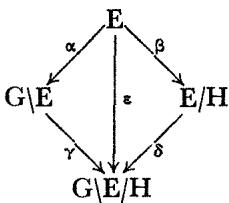
\includegraphics[keepaspectratio]{images/part001_b92675b5.jpg}}

(where \(\alpha, \beta, \gamma, \delta, \varepsilon\) denote the canonical mappings of taking quotients), \(\gamma \circ \alpha = \delta \circ \beta = \varepsilon\) .

Let G be a group and H a subgroup of G. Consider the right operation of H on G by right translation (no. 1, Example 2). The set of orbits G/H is the set of left cosets modulo H; note that G operates on G/H on the left by the law \((g, xH) \mapsto gxH\) (cf.~no. 5). Similarly, the set of right cosets modulo H is the set \(H\backslash G\) of orbits of the left operation of H on G by left translation. If K is a subgroup of G containing H and \(\Gamma\) is a left (resp. right) coset modulo H, then \(\Gamma K\) (resp. \(K\Gamma\) ) is a left (resp. right) coset modulo K. The mapping \(\Gamma \mapsto \Gamma K\) (resp. \(\Gamma \mapsto K\Gamma\) ) is called the canonical mapping of G/H into G/K (resp. of \(H\backslash G\) into \(K\backslash G\)). It is surjective.

Let G be a group and H and K two subgroups of G. Let H operate on G on the left by left translation and K on the right by right translation; these two operations commute, which allows us to consider the set \(H\backslash G/K\). The elements of \(H\backslash G/K\) are called the double cosets of G modulo H and K. When K = H, we simply say double cosets modulo H. For the canonical mapping of G/H onto \(H\backslash G/H\) to be a bijection, it is necessary and sufficient that H be a normal subgroup of G.

\subsection{HOMOGENEOUS SETS}

DEFINITION 6. Let G be a group. An operation of G on a set E is called transitive if there exists an element \(x \in E\) whose orbit is E. A G-set E is called homogeneous if the operation of G on E is transitive.

It is also said that G operates transitively on E; or that E is a homogeneous set under G. It amounts to the same to say that E is non-empty and that, for all elements x and y of E, there exists an element \(\alpha \in G\) such that \(\alpha.x = y\) .

Example. If E is a G-set, each orbit of E, with the induced operation, is a homogeneous set under G.

Let G be a group and H a subgroup of G. Consider the set G/H of left cosets modulo H. The group G operates on G/H on the left by \((g, xH) \mapsto gxH\) . Let N be the normalizer of H. The group N operates on G/H on the right by \((xH, n) \mapsto xHn = xnH\) . This operation induces on H the trivial operation and hence, on passing to the quotient, N/H operates on G/H on the right. Let \(\phi: (N/H)^{0} \to S_{G/H}\) be the homomorphism corresponding to this operation.

PROPOSITION 5. With the above notation, G/H is a homogeneous G-set. The mapping \(\phi\) induces an isomorphism of \((\mathrm{N} / \mathrm{H})^0\) onto the group of automorphisms of the G-set G/H.

The orbit in G/H of the element \(\dot{e}=H\) is G/H, whence the first assertion. We now prove the second. If \(n\in N\) defines by right translation the identity mapping on G/H, then \(\dot{e}.n=\dot{e}\) , that is H.n=H, whence \(n\in H\) . Therefore

N/H operates faithfully on G/H on the right and \(\phi\) is injective. The left operation of G and right operation of N/H on G/H commute and hence the operators of N/H define G-morphisms of G/H into itself, which are necessarily G-automorphisms since they are bijective. Therefore \(\phi\) takes its values in the group \(\Phi\) of G-automorphisms of G/H. We show that the image of \(\phi\) is \(\Phi\) . Let \(f \in \Phi\) . By transporting the structure, the stabilizer of \(f(\dot{e})\) in G is equal to the stabilizer of \(\dot{e}\) and hence to H. Let \(n \in G\) be such that \(f(\dot{e}) = n\dot{e}\) . The stabilizer of \(n\dot{e}\) in G is \(nHn^{-1}\) (no. 2, Proposition 2), whence \(nHn^{-1} = H\) and \(n \in N\) . For every element xH of G/H, \(f(xH) = f(x.\dot{e}) = x.f(\dot{e}) = xnH = xHn\) and f coincides with the mapping defined by n.

Remarks. (1) Let G be a group, H a subgroup of G and \(\phi: \mathbf{G} \to \mathfrak{S}_{\mathbf{G}/\mathbf{H}}\) the homomorphism corresponding to the operation of G on G/H. The kernel of \(\phi\) is the intersection of the conjugates of H (no. 2, Proposition 2). It is also the largest normal subgroup contained in H (no. 3). In particular, G operates faithfully on G/H if and only if the intersection of the conjugates of H reduces to \(\{e\}\) .

\begin{enumerate}
\def\labelenumi{(\arabic{enumi})}
\setcounter{enumi}{1}
\tightlist
\item
  Let G be a group and H and K subgroups such that H is a normal subgroup of K. Then K/H operates on the G-set G/H on the right and the canonical mapping of G/H onto G/K defines on passing to the quotient a G-set isomorphism \((G/H)/(K/H) \rightarrow G/K\) (cf.~no. 4).
\end{enumerate}

PROPOSITION 6. Let G be a group, E a homogeneous G-set, \(a \in E\) , H the stabilizer of \(a\) and K a subgroup of G contained in H. There exists one and only one G-morphism \(f\) of G/K into E such that \(f(e.K) = a\) . If K = H, \(f\) is an isomorphism.

If \(f\) is a solution, then \(f(x, \mathbf{K}) = x.a\) for all \(x\) in \(\mathbf{G}\) , whence the uniqueness; we show the existence. The orbital mapping defined by \(a\) is compatible with the equivalence relation \(y \in x\mathbf{K}\) on \(\mathbf{G}\) . For, if \(y = xk, k \in \mathbf{K}\) , then

\[
y. a = x k. a = x. a.
\]

A mapping \(f\) is thus derived of \(G / K\) into \(H\) which satisfies \(f(x, \mathbf{K}) = x.a\) for all \(x\) in \(G\) . This mapping is a G-morphism and \(f(\mathbf{K}) = a\) . This mapping is surjective for its image is a non-empty stable subset of \(E\) . Suppose now that \(K = H\) and let us show that \(f\) is injective. If \(f(x, \mathbf{H}) = f(y, \mathbf{H})\) , then \(x.a = y.a\) , whence \(x^{-1}y.a = a\) and \(x^{-1}y \in H\) , whence \(x.H = y.H\) .

THEOREM 1. Let G be a group.

\begin{enumerate}
\def\labelenumi{(\alph{enumi})}
\item
  Every homogeneous G-set is isomorphic to a homogeneous G-set of the form G/H where H is a subgroup of G.
\item
  Let H and H' be two subgroups of G. The G-sets G/H and G/H' are isomorphic if and only if H and H' are conjugate.
\end{enumerate}

As a homogeneous G-set is non-empty, assertion (a) follows from Proposition 6. We show (b). Let \(f: \mathrm{G} / \mathrm{H} \to \mathrm{G} / \mathrm{H}'\) be a G-set isomorphism. The subgroup H is the stabilizer of H and hence, by transport of structure, the stabilizer of an element of G/H'. The subgroups H and H' are therefore conjugate (no. 2, Proposition 2). If H' = αHα⁻¹, H' is the stabilizer of the element α. H of G/H (no. 2, Proposition 2) and hence G/H' is isomorphic to G/H (Proposition 6).

Examples. (1) Let E be a non-empty set. The group \(S_{E}\) operates transitively on E. If x and y are two elements of E, the mapping \(\tau: E \to E\) such that \(\tau(x) = y\) , \(\tau(y) = x\) and \(\tau(z) = z\) for \(z \neq x\) , y, is a permutation of E. Let \(a \in E\) . The stabilizer of a is identified with \(S_{F}\) , where \(F = E - \{a\}\) . The homogeneous G-set E is thus isomorphic to \(S_{E}/S_{F}\) .

\begin{enumerate}
\def\labelenumi{(\arabic{enumi})}
\setcounter{enumi}{1}
\tightlist
\item
  Let \(\mathbf{E}\) be a set of \(n\) elements and \((p_i)_{i\in \mathbf{I}}\) a finite family of integers \(>0\) such that \(\sum_{i}p_{i} = n\) . Let \(\mathbf{X}\) be the set of partitions \((\mathrm{F}_i)_{i\in \mathbf{I}}\) of \(\mathbf{E}\) such that \(\operatorname {Card}(\mathrm{F}_i) = p_i\) for all \(i\) . The group \(\mathfrak{S}_{\mathbf{E}}\) operates transitively on \(\mathbf{X}\) . The stabilizer H of an element \((\mathrm{F}_i)_{i\in \mathbf{I}}\) of \(\mathbf{X}\) is canonically isomorphic to \(\prod_{i\in \mathbf{I}}\mathfrak{S}_{\mathbf{F}_i}\) and is hence of order \(\prod_{i\in \mathbf{I}}p_i!\) . Applying Theorem 1 and §4, no. 4, Corollary to Proposition 4, a new proof is obtained of the fact that
\end{enumerate}

\[
\operatorname{Card} (\mathbf {X}) = \frac {n !}{\prod_ {i \in I} p _ {i} !}.
\]

In particular, take \(\mathbf{I} = \{1,2,\dots,r\}\) , \(\mathbf{E} = \{1,2,\dots,n\}\) ,

\[
\mathrm{F} _ {i} = \left\{p _ {1} + \dots + p _ {i - 1} + 1, \dots , p _ {1} + \dots + p _ {i} \right\}
\]

for \(1 \leqslant i \leqslant r\) . Let \(S\) be the set of \(\tau \in \mathfrak{S}_{E}\) such that \(\tau|_{F_i}\) is increasing for \(1 \leqslant i \leqslant r\) . If \((G_1, \ldots, G_r) \in X\) there exists one and only one \(\tau \in S\) which maps \((F_1, \ldots, F_r)\) to \((G_1, \ldots, G_r)\) . In other words, each left coset of \(\mathfrak{S}_{E}\) modulo \(H\) meets \(S\) in one and only one point.

\begin{enumerate}
\def\labelenumi{(\arabic{enumi})}
\setcounter{enumi}{2}
\tightlist
\item
  *Let \(n\) be an integer \(\geqslant 1\) . The orthogonal group \(\mathbf{O}(n, \mathbf{R})\) operates transitively on the unit sphere \(\mathbf{S}_{n-1}\) in \(\mathbf{R}^n\) . The stabilizer of the point \((0, \ldots, 0, 1)\) is identified with the orthogonal group \(\mathbf{O}(n-1, \mathbf{R})\) . The homogeneous \(\mathbf{O}(n, \mathbf{R})\) -set \(\mathbf{S}_{n-1}\) is thus isomorphic to \(\mathbf{O}(n, \mathbf{R}) / \mathbf{O}(n-1, \mathbf{R})\) .*
\end{enumerate}

\subsection{HOMOGENEOUS PRINCIPAL SETS}

DEFINITION 7. Let G be a group. An operation of G on a set E is called simply transitive if there exists an element x of E such that the orbital mapping defined by x is a bijection. A set E, together with a simply transitive left action of G on E, is called a left homogeneous principal G-set (or left homogeneous principal set under G).

It amounts to the same to say that G operates freely and transitively on E, or also that there exists an element \(x \in E\) such that the orbital mapping defined by x is an isomorphism of the G-set G (where G operates by left translation) onto E; or also that the two following conditions are satisfied:

\begin{enumerate}
\def\labelenumi{(\roman{enumi})}
\item
  E is non-empty.
\item
  for all elements \(x\) and \(y\) of \(\mathbf{E}\) , there exists one and only one element \(\alpha \in \mathbf{G}\) such that \(\alpha x = y\) .
\end{enumerate}

Condition (ii) is also equivalent to the following condition:

\begin{enumerate}
\def\labelenumi{(\roman{enumi})}
\setcounter{enumi}{2}
\tightlist
\item
  the mapping \((\alpha, x) \mapsto (\alpha x, x)\) is a bijection of \(G \times E\) onto \(E \times E\) .
\end{enumerate}

We leave to the reader the task of defining right homogeneous principal G-sets.

Examples. (1) Let G operate on itself by left (resp. right) translation. Thus a left (resp. right) homogeneous principal G-set structure is defined on G, which is sometimes denoted by \(G_{s}\) (resp. \(G_{d}\) ).

\begin{enumerate}
\def\labelenumi{(\arabic{enumi})}
\setcounter{enumi}{1}
\item
  Let E be a homogeneous set under a commutative group G. If G operates faithfully on E, the latter is a homogeneous principal G-set.
\item
  Let E and F be two isomorphic sets with structures of the same species and let \(\operatorname{Isom}(\mathbf{E}, \mathbf{F})\) be the set of isomorphisms of E onto F (with the given structures). The group \(\operatorname{Aut}(\mathbf{E})\) of automorphisms of E (with the given structure) operates on \(\operatorname{Isom}(\mathbf{E}, \mathbf{F})\) on the right by the law \((\sigma, f) \mapsto f \circ \sigma\) and \(\operatorname{Isom}(\mathbf{E}, \mathbf{F})\) is a right homogeneous principal \(\operatorname{Aut}(\mathbf{E})\) -set. Similarly, the group \(\operatorname{Aut}(\mathbf{F})\) operates on \(\operatorname{Isom}(\mathbf{E}, \mathbf{F})\) on the left by the law \((\sigma, f) \mapsto \sigma \circ f\) and \(\operatorname{Isom}(\mathbf{E}, \mathbf{F})\) is a left homogeneous principal \(\operatorname{Aut}(\mathbf{F})\) -set.
\item
  *A homogeneous principal set under the additive group of a vector space is called an affine space (cf.~II, § 9, no. 1).*
\end{enumerate}

The group of automorphisms of the homogeneous principal G-set \(G_{s}\) (Example 1) is the group of right translations of G which is identified with \(G^{0}\) (no. 5, Proposition 5). Let E be a homogeneous principal G-set and a an element of E. The orbital mapping \(\omega_{a}\) defined by a is an isomorphism of the G-set \(G_{s}\) onto E. By transporting the structure an isomorphism \(\psi_{a}\) is derived of \(G^{0}\) onto Aut(E). It should be noted that \(\psi_{a}\) in general depends on a; more precisely, for \(\alpha \in G\) ,

\[
\psi_ {\alpha a} = \psi_ {a} \circ \operatorname{Int} _ {\mathbf {G} ^ {0}} (\alpha) = \psi_ {a} \circ \operatorname{Int} (\alpha^ {- 1}).\tag{3}
\]

For, writing \(\delta_{a}\) for the translation \(x\mapsto x\alpha\) on G,

\[
\omega_ {\alpha a} = \omega_ {a} \circ \delta_ {\alpha}
\]

and

\[
\psi_ {a} (x) = \omega_ {a} \circ \delta_ {x} \circ \omega_ {a} ^ {- 1}, \quad x \in G,
\]

whence

\[
\psi_ {\alpha a} (x) = \omega_ {a} \circ \delta_ {\alpha} \circ \delta_ {x} \circ \delta_ {\alpha} ^ {- 1} \circ \omega_ {a} ^ {- 1} = \omega_ {a} \circ \delta_ {\alpha^ {- 1} x \alpha} \circ \omega_ {a} ^ {- 1} = \psi_ {a} (\alpha^ {- 1} x \alpha).
\]

\subsection{PERMUTATION GROUPS OF A FINITE SET}

If E is a finite set with n elements, the symmetric group \(S_{E}\) (§ 4, no. 1) is a finite group of order \(n!\) . When E is the interval \([1, n]\) of the set N of natural numbers, the corresponding symmetric group is denoted by \(S_{n}\) ; the symmetric group of any set with n elements is isomorphic to \(S_{n}\) .

DEFINITION 8. Let E be a finite set, \(\zeta \in \mathfrak{S}_{\mathrm{E}}\) a permutation of E and \(\bar{\zeta}\) the subgroup of \(\mathfrak{S}_{\mathrm{E}}\) generated by \(\zeta\) . \(\zeta\) is called a cycle if, under the operation of \(\bar{\zeta}\) on E, there exists one and only one orbit which is not reduced to a single element. This orbit is called the support of \(\zeta\) .

Let \(\zeta\) be a cycle. The support \(\operatorname{supp}(\zeta)\) of \(\zeta\) is the set of \(x \in E\) such that \(\zeta(x) \neq x\) .

The order of a cycle \(\zeta\) is equal to the cardinal of its support. The subgroup \(\bar{\zeta}\) generated by \(\zeta\) operates transitively and faithfully on \(\operatorname{supp}(\zeta)\) . As \(\zeta\) is commutative, \(\operatorname{supp}(\zeta)\) is a principal set under \(\bar{\zeta}\) (no. 6, Example 2) and hence \(\operatorname{Card}(\operatorname{supp}(\zeta)) = \operatorname{Card}(\bar{\zeta})\) .

Lemma 1. Let \((\zeta_{i})_{i\in I}\) be a family of cycles whose supports are pairwise disjoint. Then the \(\zeta_{i}\) are pairwise permutable. Let \(\sigma = \prod_{i\in I}\zeta_{i}\) and \(\overline{\sigma}\) be the subgroup generated by \(\sigma\) . Then \(\sigma(x) = \zeta_{i}(x)\) for \(x\in S_{i}, i\in I\) , and \(\sigma(x) = x\) for \(x\notin \bigcup_{i\in I}S_{i}\) . The mapping \(i\mapsto S_i\) is a bijection of I onto the set of \(\overline{\sigma}\) -orbits not consisting of a single element.

Let \(\zeta\) and \(\zeta'\) be two cycles whose supports are disjoint. If

\[
x \notin \operatorname{supp} (\zeta) \cup \operatorname{supp} \left(\zeta^ {\prime}\right),
\]

then \(\zeta\zeta'(x) = \zeta'\zeta(x) = x\) . If \(x\) belongs to the support of \(\zeta\) , then \(\zeta'(x) = x\) and \(\zeta(x)\) belongs to the support of \(\zeta\) , whence \(\zeta\zeta'(x) = \zeta'\zeta(x) = \zeta(x)\) . Similarly when \(x\) belongs to the support of \(\zeta'\) , then \(\zeta'\zeta(x) = \zeta\zeta'(x) = \zeta'(x)\) . Hence \(\zeta\zeta' = \zeta'\zeta\) . Therefore the \(\zeta_i\) are pairwise permutable and, for \(i \in I\) and \(x \in S_i\) , \(\sigma(x) = \zeta_i(x) \in S_i\) . The mappings \(\sigma\) and \(\zeta_i\) coincide on \(S_i\) , hence \(S_i\) is stable under \(\sigma\) and the subgroup of \(\mathfrak{S}_{S_i}\) generated by the restriction of \(\sigma\) to \(S_i\) operates transitively on \(S_i\) ; therefore \(S_i\) is a \(\overline{\sigma}\) -orbit. As the \(S_i\) are non-empty and are pairwise disjoint, the mapping \(i \mapsto S_i\) is injective. As \(\bigcup_{i} S_i\) is the set of \(x\) such that \(\sigma(x) \neq x\) , every \(\overline{\sigma}\) -orbit not consisting of a single element is one of the \(S_i\) .

PROPOSITION 7. Let E be a finite set and \(\sigma\) a permutation of E. There exists one and only one finite set C of cycles satisfying the two following conditions:

\begin{enumerate}
\def\labelenumi{(\alph{enumi})}
\item
  the supports of the elements of C are pairwise disjoints;
\item
  \(\sigma = \prod_{\zeta \in C} \zeta\) (the elements of \(C\) being pairwise permutable by Lemma 1). Let \(\bar{\sigma}\) be the subgroup generated by \(\sigma\) and let \(S\) be the set of \(\bar{\sigma}\) -orbits not consisting of a single element. For \(s \in S\) , write \(\zeta_s(x) = \sigma(x)\) if \(x \in s\) and \(\zeta_s(x) = x\) if \(x \notin s\) . For all \(s \in S\) , \(\zeta_s\) is a cycle whose support is \(s\) and \(\sigma = \prod_{s \in S} \zeta_s\) , as is seen by applying the two sides to any element of \(E\) . The uniqueness of \(C\) follows from Lemma 1.
\end{enumerate}

DEFINITION 9. A cycle of order 2 is called a transposition.

Let \(x\) and \(y\) be two distinct elements of \(E\) . Let \(\tau_{x,y}\) denote the unique transposition with support \(\{x, y\}\) .

For every permutation \(\sigma\) of E the permutation \(\sigma. \tau_{x,y}. \sigma^{-1}\) is a transposition whose support is \(\{\sigma(x), \sigma(y)\}\) . Hence:

\[
\sigma . \tau_ {x, y}. \sigma^ {- 1} = \tau_ {\sigma (x), \sigma (y)}.\tag{4}
\]

Transpositions thus form a conjugacy class in the group \(\mathfrak{S}_{\mathbb{E}}\) .

PROPOSITION 8. Let E be a finite set. The group \(\mathfrak{S}_{\mathrm{E}}\) is generated by the transpositions.

For every permutation \(\sigma\) let \(F_{\sigma}\) be the set of \(x \in E\) such that \(\sigma(x) = x\) . We show by descending induction on \(p\) that every permutation \(\sigma\) such that \(\operatorname{Card}(F_{\sigma}) = p\) is a product of transpositions. If \(p \geqslant \operatorname{Card}(E)\) , the permutation \(\sigma\) is the identity mapping of \(E\) ; it is the product of the empty family of transpositions. If \(p < \operatorname{Card}(E)\) , suppose that the property is proved for every permutation \(\sigma'\) such that \(\operatorname{Card}(F_{\sigma'}) > p\) . Now \(E - F_{\sigma} \neq \varnothing\) ; let \(x \in E - F_{\sigma}\) and \(y \in \sigma(x)\) . Then \(y \neq x\) and \(y \in E - F_{\sigma}\) . Let \(\sigma' = \tau_{x,y} \cdot \sigma\) . The set \(F_{\sigma'}\) contains \(F_{\sigma}\) and \(x\) and hence \(\operatorname{Card}(F_{\sigma'}) > \operatorname{Card}(F_{\sigma}) = p\) . By the induction hypothesis \(\sigma'\) is a product of transpositions and hence \(\sigma = \tau_{x,y} \cdot \sigma'\) is a product of transpositions.

PROPOSITION 9. Let \(n\) be an integer \(\geqslant 0\) . The group \(\mathfrak{S}_n\) is generated by the transpositions \((\tau_{i,i+1})_{1\leqslant i\leqslant n-1}\) .

By virtue of Proposition 8, it suffices to show that every transposition \(\tau_{p,q}\) , \(1 \leqslant p < q \leqslant n\) , belongs to the subgroup H generated by the \(\tau_{i,i+1}\) , \(1 \leqslant i \leqslant n-1\) . We show this by induction on \(q-p\) . For \(q-p=1\) , it is obvious. If \(q-p>1\) , then (formula (4)) \(\tau_{p,q} = \tau_{q-1,q}\tau_{p,q-1}\tau_{q-1,q}\) . By the induction hypothesis \(\tau_{p,q-1} \in H\) and therefore \(\tau_{p,q} \in H\) .

If \(\sigma \in \mathfrak{S}_n\) , every ordered pair \((i,j)\) of elements of \([1,n]\) such that \(i < j\) and \(\sigma(i) > \sigma(j)\) is called an inversion of \(\sigma\) . Let \(\nu(\sigma)\) denote the number of inversions of \(\sigma\) .

Let P be the additive group of mappings from \(Z^{n}\) to Z. For \(f \in P\) and \(\sigma \in S_{n}\) , let \(\sigma f\) be the element of P defined by

\[
\sigma f (z _ {1}, \dots , z _ {n}) = f (z _ {\sigma (1)}, \dots , z _ {\sigma (n)}).\tag{5}
\]

The action of \(\mathfrak{S}_n\) on \(\mathbf{P}\) thus defined is an operation; for all \(\sigma, \tau \in \mathfrak{S}_n\) and \(f \in \mathbf{P}, ef = f\) and

\[
\begin{array}{r l} \left(\tau (\sigma f)\right) (z _ {1}, \dots , z _ {n}) & = \sigma f (z _ {\tau (1)}, \dots , z _ {\tau (n)}) = f (z _ {\tau \sigma (1)}, \dots , z _ {\tau \sigma (n)}) \\ & = ((\tau \sigma) f) (z _ {1}, \dots , z _ {n}). \end{array}
\]

Formula (5) shows that \(\sigma(-f) = -\sigma f\) for \(\sigma \in \mathfrak{S}_n\) and \(f \in P\) .

Let \(p\) be the element of P defined by

\[
p (z _ {1}, \dots , z _ {n}) = \prod_ {i <   j} (z _ {j} - z _ {i}).\tag{6}
\]

Lemma 2. \(p \neq 0\) and \(\sigma p = (-1)^{\nu(\sigma)}\) for \(\sigma \in \mathfrak{S}_n\) .

\(p(1,2,\ldots,n) = \prod_{i < j}(j - i)\neq 0\) and hence \(p\neq 0\) . On the other hand, if \(\sigma \in \mathfrak{S}_n\) , then

\[
\sigma p (z _ {1}, \dots , z _ {n}) = p (z _ {\sigma (1)}, \dots , z _ {\sigma (n)}) = \prod_ {i <   j} (z _ {\sigma (j)} - z _ {\sigma (i)}).
\]

Let C be the set of ordered pairs \((i,j)\) such that \(1 \leqslant i \leqslant n\) , \(1 \leqslant j \leqslant n\) , i \textless{} j. A permutation \(\theta\) is defined on C by setting \(\theta(i,j) = (\sigma(i), \sigma(j))\) if \((i,j)\) is not an inversion, \(\theta(i,j) = (\sigma(j), \sigma(i))\) if \((i,j)\) is an inversion. This implies \(\sigma p = (-1)^{\nu(\sigma)} p\) .

THEOREM 2. Let E be a finite set. There exists one and only one homomorphism \(\varepsilon\) from \(\mathfrak{S}_n\) to the multiplicative group \(\{-1, +1\}\) such that \(\varepsilon(\tau) = -1\) for every transposition \(\tau\) .

The uniqueness follows from Proposition 8. We show the existence. By transporting the structure, it may be assumed that \(\mathbf{E} = [1, n]\) . Using the above notation, let \(\varepsilon(\sigma) = (-1)^{\nu(\sigma)}\) . Then (Lemma 2)

\[
\sigma (\sigma^ {\prime} p) = \sigma (\varepsilon (\sigma^ {\prime}) p) = \varepsilon (\sigma^ {\prime}) (\sigma p) = \varepsilon (\sigma^ {\prime}) \varepsilon (\sigma) p.
\]

On the other hand,

\[
\sigma (\sigma^ {\prime} p) = (\sigma \sigma^ {\prime}) p = \varepsilon (\sigma \sigma^ {\prime}) p.
\]

As \(p \neq -p\) , it follows that \(\varepsilon(\sigma\sigma') = \varepsilon(\sigma)\varepsilon(\sigma')\) and thus \(\varepsilon\) is a homomorphism. We now show that, for every transposition \(\tau, \varepsilon(\tau) = -1\) . \(\nu(\tau_{n-1,n}) = 1\) , whence \(\varepsilon(\tau_{n-1,n}) = -1\) . As every transposition \(\tau\) is conjugate to \(\tau_{n-1,n}\) and the group \(\{-1, +1\}\) is commutative, \(\varepsilon(\tau) = \varepsilon(\tau_{n-1,n}) = -1\) .

DEFINITION 10. In the notation of Theorem 2, the number \(\varepsilon(\sigma)\) (also denoted \(\varepsilon_{\sigma}\) ) is called the signature of the permutation \(\sigma\) . The kernel of the homomorphism \(\varepsilon\) is called the alternating group of E.

\(\sigma\) is called even (resp. odd) if \(\varepsilon(\sigma) = 1\) (resp. \(\varepsilon(\sigma) = -1\) ). The alternating group of E is denoted by \(\mathfrak{A}_{\mathbb{E}}\) . It is a normal subgroup of \(\mathfrak{S}_{\mathbb{E}}\) . When \(\mathbf{E} = [1, n]\) , it is simply denoted by \(\mathfrak{A}_{n}\) . When the cardinal \(n\) of E is \(\geqslant 2\) , it is a subgroup of index 2 and hence of order \(n! / 2\) . It can be shown that, for \(n = 3\) or \(n \geqslant 5\) , the group \(\mathfrak{A}_{n}\) is a simple group (cf.~Exercise 16).

Example. If \(\sigma\) is a cycle of order \(d\) , then

\[
\varepsilon (\sigma) = (- 1) ^ {d - 1}.
\]

The number of inversions of the permutation

\[
(1, 2, 3, \dots , d) \mapsto (d, 1, 2, \dots , d - 1)
\]

is equal to \(d - 1\) .

\section{EXTENSIONS, SOLVABLE GROUPS, NILPOTENT GROUPS}

Throughout this paragraph, the group laws are, unless expressly mentioned otherwise, written multiplicatively.

\subsection{EXTENSIONS}

DEFINITION 1. Let F and G be two groups. An extension of G by F is a triple \(\mathcal{E} = (\mathrm{E}, i, p)\) , where E is a group, \(i\) an injective homomorphism of F into E and \(p\) a surjective homomorphism of E onto G such that \(\operatorname{Im}(i) = \operatorname{Ker}(p)\) . A homomorphism \(s: \mathrm{G} \to \mathrm{E}\) (resp. \(r: \mathrm{E} \to \mathrm{F}\) ) such that \(p \circ s = \operatorname{Id}_{\mathbf{G}}\) (resp. \(r \circ i = \operatorname{Id}_{\mathbf{F}}\) ) is called a section (resp. retraction) of the extension \(\mathcal{E}\) .

An extension \(\mathcal{E} = (\mathrm{E}, i, p)\) of \(\mathbf{G}\) by \(\mathbf{F}\) is often denoted by the diagram \(\mathcal{E}: \mathrm{F} \xrightarrow{i} \mathrm{E} \xrightarrow{p} \mathrm{G}\) , in which \(i\) and \(p\) are sometimes omitted if no confusion can arise. It is sometimes said simply that the group \(\mathbf{E}\) is an extension of \(\mathbf{G}\) by \(\mathbf{F}\) .

For a group E to be an extension of G by F, it is necessary and sufficient that it contain a normal subgroup \(F'\) isomorphic to F such that the quotient group \(E/F'\) is isomorphic to G.

An extension \(\mathcal{E}\colon\mathrm{F}\xrightarrow{i}\mathrm{E}\xrightarrow{p}\mathrm{G}\) is called central if the image \(i(\mathrm{F})\) is contained in the centre of E; this is only possible if F is commutative.

Let \(\mathcal{E}:\mathrm{F}\xrightarrow{i}\mathrm{E}\xrightarrow{p}\mathrm{G}\) and \(\mathcal{E}':\mathrm{F}\xrightarrow{i'}\mathrm{E}'\xrightarrow{p'}\mathrm{G}\) be two extensions of G by F. A morphism of \(\mathcal{E}\) into \(\mathcal{E}'\) is a homomorphism \(u:\mathrm{E}\to\mathrm{E}'\) such that \(p'\circ u=p\) and \(u\circ i=i'\) , or, in other words, such that the following diagram is commutative:

\pandocbounded{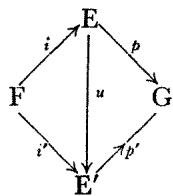
\includegraphics[keepaspectratio]{images/part001_e41623d9.jpg}}

PROPOSITION 1. Let \(\mathcal{E}: F \xrightarrow{i} E \xrightarrow{p} G\) and \(\mathcal{E}': F \xrightarrow{i'} E' \xrightarrow{p'} G\) be extensions of \(G\) by \(F\) . If \(u: E \to E'\) is a morphism of \(\mathcal{E}\) into \(\mathcal{E}'\) , \(u\) is an isomorphism of \(E\) onto \(E'\) and \(u^{-1}\) is a morphism of \(\mathcal{E}'\) into \(\mathcal{E}\) .

Let \(x \in E\) be such that \(u(x) = e\) . Then \(p(x) = p'(u(x)) = e\) , whence \(x \in i(F)\) . Let \(y \in F\) be such that \(x = i(y)\) ; then \(i'(y) = u(i(y)) = e\) . As \(i'\) is injective, \(y = e\) and \(x = e\) . Therefore \(u\) is injective. By virtue of §4, no. 6, Corollary 1 to Proposition 7, \(u\) is surjective since \(u(i(F)) = i'(F)\) . The last assertion is immediate.

In other words, the extensions \(\mathcal{E}\) and \(\mathcal{E}'\) are isomorphic if and only if there exists a morphism of \(\mathcal{E}\) into \(\mathcal{E}'\) .

Let \(\mathbf{F}\) and \(\mathbf{G}\) be two groups and write \(\mathbf{E}_0 = \mathbf{F} \times \mathbf{G}\) ; let \(i: \mathbf{F} \to \mathbf{E}_0\) be the canonical injection and \(p: \mathbf{E}_0 \to \mathbf{G}\) be the canonical projection. Every extension of \(\mathbf{G}\) by \(\mathbf{F}\) isomorphic to the extension \(\mathcal{E}_0: \mathbf{F} \xrightarrow{i} \mathbf{E}_0 \xrightarrow{p} \mathbf{G}\) is called a trivial extension.

PROPOSITION 2. Let \(\mathcal{E}:\mathrm{F}\xrightarrow{i}\mathrm{E}\xrightarrow{p}\mathrm{G}\) be an extension of \(\mathrm{G}\) by \(\mathrm{F}\) . The following conditions are equivalent:

\begin{enumerate}
\def\labelenumi{(\roman{enumi})}
\item
  \(\mathcal{E}\) is a trivial extension;
\item
  \(\mathcal{E}\) has a retraction \(r\) ;
\item
  \(\mathcal{E}\) has a section \(s\) such that \(s(\mathbf{G})\) is contained in the centralizer of \(i(\mathbf{F})\) .
\end{enumerate}

Clearly (i) implies (ii) and (iii). If (ii) holds, the mapping \((r, p): \mathbf{E} \to \mathbf{F} \times \mathbf{G}\) is a morphism of \(\mathcal{E}\) into \(\mathcal{E}_0\) , whence (i). If (iii) holds, the homomorphism of \(\mathbf{F} \times \mathbf{G}\) into \(\mathbf{E}\) corresponding to \((i, s)\) ( \(\S 4\) , no. 9, Proposition 12) is a morphism of \(\mathcal{E}_0\) into \(\mathcal{E}\) , whence (i).

It may be that an extension \(\mathcal{E}:\mathbf{F}\to\mathbf{E}\to\mathbf{G}\) is not trivial and yet the group \(\mathbf{E}\) is isomorphic to \(\mathbf{F}\times\mathbf{G}\) (Exercise 6).

DEFINITION 2. Let F and G be two groups and \(\tau\) a homomorphism of G into the automorphism group of F. Write \(\tau(g)(f) = {}^g f\) for \(g \in G\) and \(f \in F\) . The set \(\mathbf{F} \times \mathbf{G}\) with the law of composition

\[
((f, g), (f ^ {\prime}, g ^ {\prime})) \mapsto (f, g) \cdot_ {\tau} (f ^ {\prime}, g ^ {\prime}) = (f. ^ {g} f ^ {\prime}, g g ^ {\prime})\tag{1}
\]

is called the external semi-direct product of G by F relative to \(\tau\) .

The external semi-direct product of G by F relative to \(\tau\) is denoted by \(F \times_{\tau} G\) .

PROPOSITION 3. The external semi-direct product \(\mathbf{F} \times_{\tau} \mathbf{G}\) is a group. The mappings \(i: \mathbf{F} \to \mathbf{F} \times_{\tau} \mathbf{G}\) defined by \(i(f) = (f, e)\) , \(p: \mathbf{F} \times_{\tau} \mathbf{G} \to \mathbf{G}\) defined by \(p(f, g) = g\) , and \(s: \mathbf{G} \to \mathbf{F} \times_{\tau} \mathbf{G}\) defined by \(s(g) = (e, g)\) are group homomorphisms. The triple \((\mathbf{F} \times_{\tau} \mathbf{G}, i, p)\) is an extension of \(\mathbf{G}\) by \(\mathbf{F}\) and \(s\) is a section of the extension.

We have:

\[
\begin{array}{r l} ((f, g) \cdot_ {\tau} (f ^ {\prime}, g ^ {\prime})) \cdot_ {\tau} (f ^ {\prime \prime}, g ^ {\prime \prime}) & = (f. ^ {g} f ^ {\prime}, g g ^ {\prime}) \cdot_ {\tau} (f ^ {\prime \prime}, g ^ {\prime \prime}) \\ & = (f. ^ {g} f ^ {\prime}. ^ {g g ^ {\prime}} f ^ {\prime \prime}, g g ^ {\prime} g ^ {\prime \prime}); \\ (f, g) \cdot_ {\tau} ((f ^ {\prime}, g ^ {\prime}) \cdot_ {\tau} (f ^ {\prime \prime}, g ^ {\prime \prime})) & = (f, g) \cdot_ {\tau} (f ^ {\prime}. ^ {g ^ {\prime}} f ^ {\prime \prime}, g ^ {\prime} g ^ {\prime \prime}) \\ & = (f. ^ {g} (f ^ {\prime}. ^ {g ^ {\prime}} f ^ {\prime \prime}), g g ^ {\prime} g ^ {\prime \prime}). \end{array}
\]

Now \({}^{g}(f'.{}^{g'}f'') = {}^{g}f'.{}^{gg'}f''\) , which shows that the law of composition defined by (1) is associative. The element \((e, e)\) is the identity under this law. The element \((f, g)\) admits as inverse \((^{g^{-1}}f^{-1}, g^{-1})\) . Hence the law of composition on \(F \times_{\tau} G\) is a group law. The other assertions are immediate.

Using the notation of Proposition 3, \(E_{\tau}\) will denote the extension

\[
\mathrm{F} \xrightarrow {i} \mathrm{F} \times_ {\tau} \mathrm{G} \xrightarrow {p} \mathrm{G}.
\]

Let \(\mathcal{E}'\colon F\stackrel{i'}{\to}E'\stackrel{p'}{\to}G\) be an extension of \(G\) by \(F\) and \(s'\colon G\to E'\) a section of \(\mathcal{E}'\) . We define an operation \(\tau\) of \(G\) on the group \(F\) by:

\[
i ^ {\prime} (\tau (g, f)) = s ^ {\prime} (g) i ^ {\prime} (f) s ^ {\prime} (g) ^ {- 1} = \operatorname{Int} (s ^ {\prime} (g)) (i ^ {\prime} (f)).\tag{2}
\]

PROPOSITION 4. With the above notation, there exists one and only one isomorphism \(u\) of \(\mathcal{E}_{\tau}\) onto \(\mathcal{E}'\) such that \(u \circ s = s'\) .

\((f, g) = (f, e) \cdot_ {\tau} (e, g) = i(f).s(g)\) . Therefore, if u is a solution to the problem, of necessity \(u(f,g)=i'(f).s'(g)\) , whence the uniqueness of u. We prove the existence. We write \(u(f,g)=i'(f).s'(g)\) . Then

\[
\begin{array}{r l} u (f, g) \cdot u (f ^ {\prime}, g ^ {\prime}) & = i ^ {\prime} (f) s ^ {\prime} (g) i ^ {\prime} (f ^ {\prime}) s ^ {\prime} (g ^ {\prime}) \\ & = i ^ {\prime} (f) (s ^ {\prime} (g) i ^ {\prime} (f ^ {\prime}) s ^ {\prime} (g) ^ {- 1}) s ^ {\prime} (g) s ^ {\prime} (g ^ {\prime}) \\ & = i ^ {\prime} (f) i ^ {\prime} (\tau (g, f ^ {\prime})) \cdot s ^ {\prime} (g) s ^ {\prime} (g ^ {\prime}) \\ & = i ^ {\prime} (f \cdot \tau (g, f ^ {\prime})) \cdot s ^ {\prime} (g g ^ {\prime}) \\ & = u ((f, g) \cdot_ {\tau} (f ^ {\prime}, g ^ {\prime})). \end{array}
\]

Therefore, \(u\) is a homomorphism of \(\mathbf{F} \times_{\tau} \mathbf{G}\) into \(\mathbf{E}'\) . Obviously \(u \circ i = i'\) , \(p' \circ u = p\) and \(u \circ s = s'\) .

Remark. The definition of the operation \(\tau\) by formula (2) depends on the extension \(\mathcal{E}'\) and the section \(s'\) . When F is commutative, the operation \(\tau\) does not depend on \(s'\) . For \(\operatorname{Int}(s'(g)) \mid i'(F)\) depends then only on the coset of \(s'(g)\) mod. \(i'(F)\) .

More generally, let \(\mathcal{E}:\mathrm{F}\to \mathrm{E}\to \mathrm{G}\) be an extension of \(\mathbf{G}\) by a commutative group \(\mathbf{F}\) (it is not assumed that \(\mathcal{E}\) admits a section). The group \(\mathbf{E}\) operates on \(\mathbf{F}\) by inner automorphisms, this image is trivial on the image of \(\mathbf{F}\) and hence defines an operation of \(\mathbf{G}\) on \(\mathbf{F}\) . If \(\mathcal{E}\) admits a section, this operation is that defined by formula (2).

COROLLARY. Let G be a group and H and K two subgroups of G such that H is normal, \(\mathbf{H} \cap \mathbf{K} = \{e\}\) and \(\mathbf{H} \cdot \mathbf{K} = \mathbf{G}\) . Let \(\tau\) be the operation of \(\mathbf{K}\) on \(\mathbf{H}\) by inner automorphisms of \(\mathbf{G}\) . The mapping \((h, k) \mapsto hk\) is an isomorphism of \(\mathbf{H} \times_{\tau} \mathbf{K}\) onto \(\mathbf{G}\) .

Under the hypotheses of this corollary, G is said to be the semi-direct product of K by H.

Examples. (1) Let G be a group and E a homogeneous principal G-set; let \(\Gamma\) denote the automorphism group of G. Let A be the set of permutations f of E with the following property:

There exists \(\gamma \in \Gamma\) such that \(f\) is a \(\gamma\) -morphism of \(\mathbf{E}\) into \(\mathbf{E}\) (that is, \(f(gb) = \gamma(g)f(b)\) for \(b \in \mathbf{E}\) and \(g \in \mathbf{G}\) ).

The above formula \(f(gb) = \gamma(g)f(b)\) shows that if \(f \in A\) there exists a unique \(\gamma \in \Gamma\) such that \(f\) is a \(\gamma\) -morphism, we shall denote it by \(p(f)\) .

Let \(f, f'\) be in A, \(\gamma = p(f), \gamma' = p(f')\) . Then, for all \(b \in E\) and all \(g \in G\) ,

\[
(f ^ {\prime} \circ f) (g b) = f ^ {\prime} (\gamma (g) f (b)) = \gamma^ {\prime} (\gamma (g)) f ^ {\prime} (f (b))
\]

which proves that \(f' \circ f \in \mathbf{A}\) and that \(p(f' \circ f) = p(f')p(f)\) . On the other hand, \(f(\gamma^{-1}(g)f^{-1}(b)) = gb\) , whence \(f^{-1}(gb) = \gamma^{-1}(g)f^{-1}(b)\) and \(f^{-1} \in \mathbf{A}\) . Thus \(\mathbf{A}\) is a subgroup of \(\mathfrak{S}_{\mathbf{E}}\) and \(p\) is a homomorphism of \(\mathbf{A}\) into \(\Gamma\) . The kernel of \(p\) is the set \(\operatorname{Aut}_{\mathbf{G}}(\mathbf{E})\) of automorphisms of the \(\mathbf{G}\) -set \(\mathbf{E}\) .

We fix \(a \in \mathbf{E}\) . We have defined in § 5, no. 6 an isomorphism \(\psi_a\) of \(\mathbf{G}^0\) onto \(\operatorname{Aut}_{\mathbf{G}}(\mathbf{E})\) such that \(\psi_a(x)(ga) = gxa\) for all \(g, x\) in \(\mathbf{G}\) . On the other hand, for \(\gamma \in \Gamma\) , let \(s_a(\gamma)\) be the permutation of \(\mathbf{E}\) defined by \(s_a(\gamma)(ga) = \gamma(g)a\) for all \(g \in \mathbf{G}\) ; it is immediately verified that \(s_a\) is a homomorphism of \(\Gamma\) into \(\mathbf{A}\) such that \(p \circ s_a = \operatorname{Id}_{\Gamma}\) . Thus \(\mathbf{G}^0 \xrightarrow{\psi_a} \mathbf{A} \xrightarrow{p} \Gamma\) is an extension of \(\Gamma\) by \(\mathbf{G}^0\) and \(s_a\) is a section of this extension. This extension and this section define an operation of \(\Gamma\) on \(\mathbf{G}^0\) , \(s_a(\Gamma)\) acting on \(\psi_a(\mathbf{G}^0)\) by inner automorphisms; we write this operation exponentially. We show that this operation is the natural operation (§ 3, no. 1, Example 3): for \(x, g\) in \(\mathbf{G}\) and \(\gamma \in \Gamma\) ,

\[
\begin{array}{r l} (\psi_ {a} (^ {\gamma} x)) (g a) & = (s _ {a} (\gamma) \circ \psi_ {a} (x) \circ s _ {a} (\gamma) ^ {- 1}) (g a) \\ & = (s _ {a} (\gamma) \circ \psi_ {a} (x)) (\gamma^ {- 1} (g) a) = s _ {a} (\gamma) (\gamma^ {- 1} (g) x a) \\ & = g \gamma (x) a = \psi_ {a} (\gamma (x)) g a \end{array}
\]

whence \({}^{\gamma}x = \gamma(x)\) .

Proposition 4 then shows that A is isomorphic to the semidirect product of \(\Gamma = \operatorname{Aut}(\mathbf{G})\) by \(\mathbf{G}^0\) under the natural operation of \(\operatorname{Aut}(\mathbf{G})\) on \(\mathbf{G}^0\) . Note that the isomorphism which we have constructed depends in general on the choice of the element \(a \in \mathbf{E}\) .

\begin{enumerate}
\def\labelenumi{(\arabic{enumi})}
\setcounter{enumi}{1}
\tightlist
\item
  *Let A be a commutative ring. The upper triangular group T(n, A) is the semi-direct product of the diagonal subgroup D(n, A) by the upper strict triangular group T1(n, A).*
\end{enumerate}

\subsection{COMMUTATORS}

DEFINITION 3. Let G be a group and x and y two elements of G. The element \(x^{-1}y^{-1}xy\) of G is called the commutator of x and y.

\((x,y)\) is used to denote the commutator of x and y. Then obviously

\[
(y, x) = (x, y) ^ {- 1}.
\]

For \(x\) and \(y\) to commute it is necessary and sufficient that \((x, y) = e\) . More generally,

\[
x y = y x (x, y).
\]

On the other hand we write

\[
x ^ {y} = y ^ {- 1} x y = x (x, y) = (y, x ^ {- 1}) x.\tag{3}
\]

As the mapping \(x \mapsto x^y\) is the inner automorphism \(\operatorname{Int}(y^{-1})\) , \((x, y)^z = (x^z, y^z)\) for all \(x, y, z \in G\) .

For \(x, y, z \in G\) , we prove the following relations:

\[
(x, y z) = (x, z). (x, y) ^ {z} = (x, z). (z, (y, x)). (x, y)\tag{4}
\]

(4 bis) \((xy,z) = (x,z)^y.(y,z) = (x,z).(((x,z),y).(y,z))\)

\begin{enumerate}
\def\labelenumi{(\arabic{enumi})}
\setcounter{enumi}{4}
\item
  \((x^{y}, (y, z)).(y^{z}, (z, x)).(z^{x}, (x, y)) = e\)
\item
  \((x, yz).(z, xy).(y, zx) = e\)
\end{enumerate}

(6 bis) \((xy, z). (yz, x). (zx, y) = e.\)

Now

\[
\begin{array}{r l} (x, y z) & = x ^ {- 1} z ^ {- 1} y ^ {- 1} x y z = (x, z) z ^ {- 1} x ^ {- 1} y ^ {- 1} x y z = (x, z) (x, y) ^ {z} \\ & = (x, z) (z, (x, y) ^ {- 1}) (x, y) \end{array}
\]

by (3), which proves (4). Formula (4 bis) follows similarly. On the other hand,

\[
\begin{array}{r l} (x ^ {y}, (y, z)) & = (x ^ {y}) ^ {- 1} (z, y) (x ^ {y}) (y, z) \\ & = y ^ {- 1} x ^ {- 1} y z ^ {- 1} y ^ {- 1} z y y ^ {- 1} x y y ^ {- 1} z ^ {- 1} y z \\ & = (y z y ^ {- 1} x y) ^ {- 1} (z x z ^ {- 1} y z). \end{array}
\]

Then writing \(u = yzy^{-1}xy\) , \(v = zxz^{-1}yz\) and \(w = xyx^{-1}zx\) , we obtain

\[
(x ^ {y}, (y, z)) = u ^ {- 1} v.
\]

By cyclically permuting \(x, y, z\) , we deduce \((y^z, (z, x)) = v^{-1}w\) and

\[
\left(z ^ {x}, (x, y)\right) = w ^ {- 1} u,
\]

which immediately imply (5). Finally, (6) follows by multiplying together the two sides in the three formulae obtained by cyclically permuting x, y, z in the formula \((x, yz) = x^{-1}z^{-1}y^{-1}xyz = (yzx)^{-1}(xyz)\) , and similarly for (6 bis).

If A and B are two subgroups of G, (A, B) denotes the subgroup generated by the commutators \((a, b)\) with \(a \in A\) and \(b \in B\) . Then \((A, B) = \{e\}\) if and only if A centralizes B. \((A, B) \subset A\) if and only if B normalizes A. If A and B are normal (resp. characteristic), so is \((A, B)\) .

PROPOSITION 5. Let A, B, C be three subgroups of G.

\begin{enumerate}
\def\labelenumi{(\roman{enumi})}
\item
  The subgroup A normalizes the subgroup (A, B).
\item
  If the subgroup (B, C) normalizes A, the subgroup (A, (B, C)) is generated by the elements \((a, (b, c))\) with \(a \in \mathbf{A}\) , \(b \in \mathbf{B}\) and \(c \in \mathbf{C}\) .
\item
  If A, B and C are normal, then
\end{enumerate}

\[
(\mathrm{A}, (\mathrm{B}, \mathrm{C})) \subset (\mathrm{C}, (\mathrm{B}, \mathrm{A})). (\mathrm{B}, (\mathrm{C}, \mathrm{A})).
\]

By (4 bis), for \(a, a' \in \mathbf{A}\) and \(b \in \mathbf{B}\) ,

\[
(a, b) ^ {a ^ {\prime}} = (a a ^ {\prime}, b). (a ^ {\prime}, b) ^ {- 1},
\]

whence (i). Suppose now that (B, C) normalizes A. For \(a \in \mathbf{A}\) , \(b \in \mathbf{B}\) , \(c \in \mathbf{C}\) and \(x \in \mathbf{G}\) , (4) implies

\[
(a, (b, c). x) = (a, x). (x, ((b, c), a)) (a, (b, c))
\]

and \(((b, c), a) \in \mathbf{A}\) since (B, C) normalizes A, whence by induction on \(p\) the fact that \(\left(a, \prod_{i=1}^{p} (b_i, c_i)\right)\) , for \(b_i \in \mathbf{B}\) , \(c_i \in \mathbf{C}\) , belongs to the subgroup generated by the elements of the form \((a, (b, c))\) . If finally A, B and C are normal, so are the subgroups (A, (B, C)), (C, (B, A)) and (B, (C, A)). It therefore suffices by (ii) to show that

\[
(a, (b, c)) \in (\mathrm{C}, (\mathrm{B}, \mathrm{A})). (\mathrm{B}, (\mathrm{C}, \mathrm{A}))
\]

for all \(a \in \mathbf{A}\) , \(b \in \mathbf{B}\) and \(c \in \mathbf{C}\) . Now by (5), writing \(a^{b^{-1}} = u\)

\[
(a, (b, c)) = ((u ^ {b}), (b, c)) = (c ^ {u}, (u, b)) ^ {- 1}. (b ^ {c}, (c, u)) ^ {- 1},
\]

whence (iii).

DEFINITION 4. Let G be a group. The subgroup generated by the commutators of elements of G is called the derived group of G.

The derived group of G is thus the subgroup (G, G). It is also denoted by D(G). By an abuse of language, it is sometimes called the commutator group of G although it is in general distinct from the set of commutators of elements of G (Exercise 16). D(G) = \{e\} if and only if G is commutative.

PROPOSITION 6. Let \(f: \mathbf{G} \to \mathbf{G}'\) be a group homomorphism. Then \(f(\mathbf{D}(\mathbf{G})) \subset \mathbf{D}(\mathbf{G}')\) . If \(f\) is surjective, the homomorphism of \(\mathbf{D}(\mathbf{G})\) into \(\mathbf{D}(\mathbf{G}')\) the restriction of \(f\) is surjective.

The image under \(f\) of a commutator of elements of \(G\) is a commutator of elements of \(G'\) . If \(f\) is surjective, the image under \(f\) of the set of commutators of \(G\) is the set of commutators of \(G'\) . The proposition thus follows from § 4, no. 3, Corollary 3 to Proposition 2.

COROLLARY 1. The derived group of a group G is a characteristic subgroup of G. In particular it is a normal subgroup of G.

COROLLARY 2. Let G be a group. The quotient group G/D(G) is commutative. Let \(\pi: G \to G/D(G)\) be the canonical homomorphism. Every homomorphism \(f\) of G into a commutative group \(G'\) can be expressed uniquely in the form \(f = \bar{f} \circ \pi\) , where \(\bar{f}: G/D(G) \to G'\) is a homomorphism.

Now \(\pi (\mathbf{D}(\mathbf{G})) = \{e\}\) . As \(\pi\) is surjective, it follows that \(\mathbf{D}(\mathbf{G} / \mathbf{D}(\mathbf{G})) = \{e\}\) , whence the first assertion. The second follows from § 4, no. 4, Proposition 5.

COROLLARY 3. Let H be a subgroup of G. The following conditions are equivalent:

\begin{enumerate}
\def\labelenumi{(\roman{enumi})}
\item
  \(\mathbf{H} \supset \mathbf{D}(\mathbf{G})\) ;
\item
  H is a normal subgroup and G/H is commutative.
\item
  (ii) \(\Rightarrow\) (i) by Corollary 2 and (i) \(\Rightarrow\) (ii) by §4, no. 7, Theorem 4, since every subgroup of a commutative group is normal.
\end{enumerate}

COROLLARY 4. Let G be a group and X a subset of G which generates G. The group D(G) is the normal subgroup of G generated by the commutators of elements of X.

Let H be the normal subgroup of G generated by the commutators of elements of X and \(\phi: G \to G/H\) the canonical homomorphism. The set \(\phi(X)\) generates G/H. The elements of \(\phi(X)\) are pairwise permutable and hence H is commutative ( \(\S 4\) , no. 3, Corollary 2 to Proposition 2). Hence (Corollary 3) H contains D(G). On the other hand, obviously \(H \subset D(G)\) .

Remarks. (1) Corollary 2 can also be expressed by saying that G/D(G), together with \(\pi\) , is a solution of the universal mapping problem for G, relative to commutative groups and homomorphisms from G to commutative groups.

\begin{enumerate}
\def\labelenumi{(\arabic{enumi})}
\setcounter{enumi}{1}
\tightlist
\item
  Under the hypotheses of Corollary 4, the subgroup generated by the commutators of elements of X is contained in D(G) but is not in general equal to D(G) (cf.~Exercise 15e).
\end{enumerate}

Examples. (1) If \(\mathbf{G}\) is a non-commutative simple group, then \(\mathrm{D}(\mathbf{G}) = \mathbf{G}\) . Therefore every homomorphism of \(\mathbf{G}\) into a commutative group is trivial.

\begin{enumerate}
\def\labelenumi{(\arabic{enumi})}
\setcounter{enumi}{1}
\tightlist
\item
  The derived group of the symmetric group \(\mathfrak{S}_n\) is the alternating group \(\mathfrak{A}_n\) . For \(\mathfrak{A}_n\) is generated by the products of two transpositions; if \(\tau = \tau_{x,y}\) and \(\tau' = \tau_{x',y'}\) are two transpositions, let \(\sigma\) be a permutation such that \(\sigma(x') = x\) and \(\sigma(y') = y\) . Then \(\tau' = \sigma^{-1}\tau\sigma\) and \(\tau\tau' = \tau^{-1}\tau' = \tau^{-1}\sigma^{-1}\tau\sigma\) is a commutator. Hence \(\mathfrak{A}_n \subset D(\mathfrak{S}_n)\) . As \(\mathfrak{S}_n / \mathfrak{A}_n\) is commutative, \(\mathfrak{A}_n \supset D(\mathfrak{S}_n)\) (Corollary 3).
\end{enumerate}

\subsection{LOWER CENTRAL SERIES, NILPOTENT GROUPS}

Let \(\mathbf{G}\) be a group, \(\mathbf{H}\) a subgroup of \(\mathbf{G}\) and \(\mathbf{K}\) a normal subgroup of \(\mathbf{G}\) . The image of \(\mathbf{H}\) in \(\mathbf{G} / \mathbf{K}\) is contained in the centre of \(\mathbf{G} / \mathbf{K}\) if and only if \((\mathbf{G}, \mathbf{H}) \subset \mathbf{K}\) .

DEFINITION 5. Let G be a group. The lower central series of G is the sequence \((\mathbf{C}^n (\mathbf{G}))_{n\geqslant 1}\) of subgroups of G defined inductively by:

\[
\mathbf {C} ^ {1} (\mathbf {G}) = \mathbf {G}, \quad \mathbf {C} ^ {n + 1} (\mathbf {G}) = (\mathbf {G}, \mathbf {C} ^ {n} (\mathbf {G})).
\]

Let \(f: \mathbf{G} \to \mathbf{G}'\) be a group homomorphism. It is seen, by induction on \(n\) , that \(f(\mathbf{C}^n(\mathbf{G})) \subset \mathbf{C}^n(\mathbf{G}')\) and that, if \(f\) is surjective, \(f(\mathbf{C}^n(\mathbf{G})) = \mathbf{C}^n(\mathbf{G}')\) . In particular, for all \(n \geqslant 1\) , \(\mathbf{C}^2(\mathbf{G})\) is a characteristic (and hence normal) subgroup of \(\mathbf{G}\) . For all \(n \geqslant 1\) , \(\mathbf{C}^n(\mathbf{G}) / \mathbf{C}^{n+1}(\mathbf{G})\) is contained in the centre of \(\mathbf{G} / \mathbf{C}^{n+1}(\mathbf{G})\) .

Let \((\mathbf{G}_1, \mathbf{G}_2, \ldots)\) be a decreasing sequence of normal subgroups of \(\mathbf{G}\) such that (1) \(\mathbf{G}_1 = \mathbf{G}\) ; (2) for all \(i\) , \(\mathbf{G}_i / \mathbf{G}_{i+1}\) is contained in the centre of \(\mathbf{G} / \mathbf{G}_{i+1}\) . Then \(\mathbf{C}^i(\mathbf{G}) \subset \mathbf{G}_i\) , as is seen by induction on \(i\) .

Now

\[
\left(\mathbf {C} ^ {m} (\mathbf {G}), \mathbf {C} ^ {n} (\mathbf {G})\right) \subset \mathbf {C} ^ {m + n} (\mathbf {G}).\tag{7}
\]

For, if this relation is denoted by \((\mathbf{F}_{m,n})\) , it follows from \((\mathbf{F}_{m,n})\) , by no. 2, Proposition 5, that

\[
\begin{array}{l} \left(\mathrm{C} ^ {m} (\mathrm{G}), \mathrm{C} ^ {n + 1} (\mathrm{G})\right) \subset \left(\mathrm{G}, \left(\mathrm{C} ^ {m} (\mathrm{G}), \mathrm{C} ^ {n} (\mathrm{G})\right)\right). \left(\mathrm{C} ^ {n} (\mathrm{G}), \left(\mathrm{G}, \mathrm{C} ^ {m} (\mathrm{G})\right)\right) \\ \subset \mathrm{C} ^ {m + n + 1} (\mathrm{G}). \left(\mathrm{C} ^ {m + 1} (\mathrm{G}), \mathrm{C} ^ {n} (\mathrm{G})\right). \end{array}
\]

Hence \(((\mathbf{F}_{m,n})\) and \((\mathbf{F}_{m + 1,n}))\Rightarrow (\mathbf{F}_{m,n + 1})\) . As \((\mathbf{F}_{m,1})\) and \((\mathbf{F}_{1,n})\) are obvious \((\mathbf{F}_{m,n})\) follows by induction.

DEFINITION 6. A group G is called nilpotent if there exists an integer n such that \(\mathbf{C}^{n+1}(\mathbf{G}) = \{e\}\) . The least integer n such that \(\mathbf{C}^{n+1}(\mathbf{G}) = \{e\}\) is called the nilpotency class of a nilpotent group G.

If \(n \in N\) , a group of nilpotency class n is called a nilpotent group of class n.~It is sometimes said that the nilpotency class of a group G is finite if G is nilpotent.

Examples. (1) A group is nilpotent of class 0 (resp. \(\leqslant 1\) ) if and only if it consists of the identity element (resp. is commutative).

\begin{enumerate}
\def\labelenumi{(\arabic{enumi})}
\setcounter{enumi}{1}
\item
  *For every commutative ring A and every integer \(n \geqslant 1\) , the upper strict triangular group \(\mathrm{T}_1(n, \mathbf{A})\) is nilpotent of class \(\leqslant n - 1\) (and exactly of class \(n - 1\) if \(\mathbf{A} \neq \{0\}\) ).*
\item
  Let \(\mathbf{G}\) be a nilpotent group of class \(n\) . Every subgroup (resp. every quotient group) of \(\mathbf{G}\) is nilpotent of class \(\leqslant n\) . For, if \(\mathbf{H}\) is a subgroup of \(\mathbf{G}\) , then \(\mathbf{C}^n (\mathbf{H})\subset \mathbf{C}^n (\mathbf{G})\) . If \(\mathbf{G}'\) is a quotient group of \(\mathbf{G}\) and \(\pi : \mathbf{G}\to \mathbf{G}'\) is the canonical homomorphism, then \(\mathbf{C}^n (\mathbf{G}') = \pi (\mathbf{C}^n (\mathbf{G}))\) .
\item
  A finite product of nilpotent groups is nilpotent.
\end{enumerate}

PROPOSITION 7. Let G be a group and n an integer. The following conditions are equivalent:

\begin{enumerate}
\def\labelenumi{(\alph{enumi})}
\item
  G is nilpotent of class \(\leqslant n\) .
\item
  There exists a series of subgroups of \(\mathbf{G}\) :
\end{enumerate}

\[
\mathrm{G} = \mathrm{G} ^ {1} \supset \mathrm{G} ^ {2} \supset \dots \supset \mathrm{G} ^ {n + 1} = \{e \}
\]

such that \((\mathbf{G},\mathbf{G}^k)\subset \mathbf{G}^{k + 1}\) for all \(k\in [1,n]\) .

\begin{enumerate}
\def\labelenumi{(\alph{enumi})}
\setcounter{enumi}{2}
\item
  There exists a subgroup \(\mathbf{A}\) of \(\mathbf{G}\) contained in the centre of \(\mathbf{G}\) such that \(\mathbf{G} / \mathbf{A}\) is nilpotent of class \(\leqslant n - 1\) .
\item
  (a) \(\Rightarrow\) (b): it suffices to take \(\mathbf{G}^k = \mathbf{C}^k (\mathbf{G})\) .
\item
  (b) \(\Rightarrow\) (a): by induction on \(k\) , \(\mathbf{C}^k (\mathbf{G})\subset \mathbf{G}^k\)
\item
  (a) \(\Rightarrow\) (c): it suffices to take \(\mathbf{A} = \mathbf{C}^n (\mathbf{G})\) .
\item
  (c) \(\Rightarrow\) (a): let \(\pi: \mathbf{G} \to \mathbf{G} / \mathbf{A}\) be the canonical homomorphism; then \(\pi(\mathbf{C}^n(\mathbf{G})) = \mathbf{C}^n(\mathbf{G} / \mathbf{A}) = \{e\}\) and hence \(\mathbf{C}^n(\mathbf{G}) \subset \mathbf{A}\) , whence \(\mathbf{C}^{n+1}(\mathbf{G}) = \{e\}\) .
\end{enumerate}

More briefly: a group is nilpotent of class \(\leqslant n\) if it can be obtained from the group \(\{e\}\) by n successive central extensions.

COROLLARY. A central extension of a nilpotent group (by a necessarily commutative group) is nilpotent.

PROPOSITION 8. Let G be a nilpotent group of class \(\leqslant n\) and let H be a subgroup of G. There exists a sequence of subgroups

\[
\mathbf {G} = \mathbf {H} ^ {1} \supset \mathbf {H} ^ {2} \supset \dots \supset \mathbf {H} ^ {n + 1} = \mathbf {H},
\]

such that \(\mathbf{H}^{k + 1}\) is normal in \(\mathbf{H}^k\) and \(\mathbf{H}^k /\mathbf{H}^{k + 1}\) is commutative for all \(k\leqslant n\)

Choose a sequence \((\mathbf{G}^{k})\) of subgroups of G satisfying the conditions of Proposition 7 (b) for all k; \(G^{k}\) is normal in G. Write:

\[
\mathbf {H} ^ {k} = \mathbf {H}. \mathbf {G} ^ {k}.
\]

It is necessary to verify that \(\mathbf{H}^{k + 1}\) is normalized by \(\mathbf{H}^k = \mathbf{H}.\mathbf{G}^k\) ; as it is normalized by \(\mathbf{H}\) , it suffices to verify that it is by \(\mathbf{G}^k\) . Now, if \(s\in \mathbf{G}^k\) and \(h\in \mathbf{H}\) ,

\[
s h s ^ {- 1} = s h s ^ {- 1} h ^ {- 1}. h \in (\mathrm{G}, \mathrm{G} ^ {k}). \mathrm{H}
\]

and \((\mathbf{G},\mathbf{G}^k)\) . H is contained in \(\mathbf{G}^{k + 1}\) . \(\mathbf{H} = \mathbf{H}^{k + 1}\) ; hence \(s.\mathbf{H}^{k + 1}.s^{-1} = \mathbf{H}^{k + 1}\) , which shows that \(\mathbf{H}^{k + 1}\) is normal in \(\mathbf{H}^k\) .

Finally, the canonical homomorphism \(G^{k}/G^{k+1} \to H^{k}/H^{k+1}\) is obviously surjective; as the first group is commutative, so is the second.

COROLLARY 1. Let G be a nilpotent group and H a subgroup of G. If H is distinct from G, the normalizer \(N_{G}(H)\) of H in G is distinct from H.

Let \(k\) be the largest index such that \(H^{k} \neq H\) . The group \(H^{k}\) normalizes \(H\) and is distinct from \(H\) .

COROLLARY 2. Let G be a nilpotent group and H a subgroup of G. If H is distinct from G, there exists a normal subgroup N of G, containing H, distinct from G and such that G/N is commutative.

Let \(k\) be the least index such that \(H^k \neq G\) . The group \(H^k\) satisfies the required conditions.

COROLLARY 3. Let G be a nilpotent group and H a subgroup of G. If G = H.(G, G), then G = H.

Every subgroup N of G which contains H and such that G/N is commutative contains H.(G, G). Corollary 3 thus follows from Corollary 2.

Corollary 3 can also be formulated thus: let X be a subset of G. For X to generate G, it is necessary and sufficient that the image of X in G/D(G) generate G/D(G).

COROLLARY 4. Let \(f: \mathbf{G}' \to \mathbf{G}\) be a group homomorphism. Suppose that

\begin{enumerate}
\def\labelenumi{(\alph{enumi})}
\item
  G is nilpotent.
\item
  The homomorphism \(f_1 \colon \mathbf{G}' / (\mathbf{G}', \mathbf{G}') \to \mathbf{G} / (\mathbf{G}, \mathbf{G})\) , derived from \(f\) by passing to the quotients, is surjective.
\end{enumerate}

Then \(f\) is surjective.

This follows from Corollary 3 applied to the subgroup \(\mathbf{H} = f(\mathbf{G}')\) .

PROPOSITION 9. Let G be a nilpotent group of class \(\leqslant n\) and let N be a normal subgroup of G. There exists a series of subgroups

\[
\mathrm{N} = \mathrm{N} ^ {1} \supset \mathrm{N} ^ {2} \supset \dots \supset \mathrm{N} ^ {n + 1} = \{e \}
\]

such that \((\mathbf{G},\mathbf{N}^k)\subset \mathbf{N}^{k + 1}\) for \(k = 1,\dots ,n\)

If \((\mathbf{G}^k)\) satisfies condition (b) of Proposition 7, then take

\[
\mathbf {N} ^ {k} = \mathbf {G} ^ {k} \cap \mathbf {N}.
\]

COROLLARY 1. Let G be a nilpotent group, Z the centre of G and N a normal subgroup of G. If N ≠ \{e\}, then N ∩ Z ≠ \{e\}.

Let \(k\) be the largest index such that \(\mathbf{N}^k \neq \{e\}\) . The group \(\mathbf{N}^k\) is contained in \(\mathbf{N}\) . On the other hand, \((\mathbf{G}, \mathbf{N}^k) \subset \mathbf{N}^{k+1} = \{e\}\) ; hence \(\mathbf{N}^k\) is contained in the centre \(\mathbf{Z}\) of \(\mathbf{G}\) .

COROLLARY 2. Let \(f\) be a homomorphism from a nilpotent group \(G\) to a group \(G'\) . If the restriction of \(f\) to the centre of \(G\) is injective, \(f\) is injective.

This is Corollary 1 applied to \(\operatorname{Ker}(f)\) .

\subsection{DERIVED SERIES, SOLVABLE GROUPS}

DEFINITION 7. Let G be a group. The derived series of G is the series \((\mathbf{D}^n (\mathbf{G}))_{n\in \mathbb{N}}\) defined inductively by:

\[
\mathbf {D} ^ {0} (\mathbf {G}) = \mathbf {G}; \quad \mathbf {D} ^ {n + 1} (\mathbf {G}) = \mathbf {D} (\mathbf {D} ^ {n} (\mathbf {G})) \quad \text { for } n \in \mathbf {N}.
\]

Then \(\mathbf{D}^0 (\mathbf{G}) = \mathbf{C}^1 (\mathbf{G}) = \mathbf{G},\mathbf{D}^1 (\mathbf{G}) = \mathbf{C}^2 (\mathbf{G}) = \mathbf{D}(\mathbf{G}) = (\mathbf{G},\mathbf{G}).\) For all \(n \in \mathbf{N}, \mathrm{D}^n(\mathrm{G}) \subset \mathrm{C}^{2^n}(\mathrm{G})\) , as is seen by induction on \(n\) using formula (7) of no. 3.

Let \(f: \mathbf{G} \to \mathbf{G}'\) be a group homomorphism. It is seen, by induction on \(n\) , that \(f(\mathbf{D}^n(\mathbf{G})) \subset \mathbf{D}^n(\mathbf{G}')\) and that, if \(f\) is surjective, \(f(\mathbf{D}^n(\mathbf{G})) = \mathbf{D}^n(\mathbf{G}')\) . In particular, for all \(n \in \mathbf{N}\) , \(\mathbf{D}^n(\mathbf{G})\) is a characteristic (and therefore normal) subgroup of \(\mathbf{G}\) . For all \(n \in \mathbf{N}\) , the group \(\mathbf{D}^n(\mathbf{G}) / \mathbf{D}^{n+1}(\mathbf{G})\) is a commutative normal (but not in general central) subgroup of \(\mathbf{G} / \mathbf{D}^{n+1}(\mathbf{G})\) .

Let \((\mathbf{G}_0, \mathbf{G}_1, \ldots)\) be a decreasing sequence of subgroups of \(\mathbf{G}\) such that: (1) \(\mathbf{G}_0 = \mathbf{G}\) ; (2) for all \(i\) , \(\mathbf{G}_{i+1}\) is normal in \(\mathbf{G}_i\) and \(\mathbf{G}_i / \mathbf{G}_{i+1}\) is commutative. Then \(\mathbf{D}^i(\mathbf{G}) \subset \mathbf{G}_i\) for all \(i\) , as is seen by induction on \(i\) .

DEFINITION 8. A group G is called solvable if there exists an integer n such that \(\mathbf{D}^{n}(\mathbf{G})=\{e\}\) . If G is a solvable group, the least integer n such that \(\mathbf{D}^{n}(\mathbf{G})=\{e\}\) is called the solvability class of G.

A solvable group of solvability class n is called a solvable group of class n.~A group is sometimes said to be of finite solvability class if it is solvable.

Examples. (1) A group is solvable of class 0 (resp. \(\leqslant 1\) ) if and only if it is reduced to \(\{e\}\) (resp. is commutative).

\begin{enumerate}
\def\labelenumi{(\arabic{enumi})}
\setcounter{enumi}{1}
\item
  Every nilpotent group of class \(\leqslant 2^{n} - 1\) is solvable of class \(\leqslant n\) ; this follows from the relation \(\mathbf{D}^n (\mathbf{G})\subset \mathbf{C}^{2^n}(\mathbf{G})\) proved above.
\item
  Let G be a solvable group of class \(\leqslant n\) . Every subgroup (resp. quotient group) of G is solvable of class \(\leqslant n\) (proof analogous to that of no. 3, Example 3).
\item
  If \(\mathbf{G}\) is a solvable group of class \(p\) and \(\mathbf{F}\) is a solvable group of class \(q\) , every extension \(\mathbf{E}\) of \(\mathbf{G}\) by \(\mathbf{F}\) is a solvable group of class \(\leqslant p + q\) . For, let \(\pi: \mathbf{E} \to \mathbf{G}\) be the projection; then \(\pi(\mathrm{D}^p(\mathbf{E})) \subset \mathrm{D}^p(\mathbf{G}) = \{e\}\) and therefore \(\mathrm{D}^p(\mathbf{E}) \subset \mathbf{F}\) ; it follows that \(\mathrm{D}^{p+q}(\mathbf{E}) = \mathrm{D}^q(\mathrm{D}^p(\mathbf{E})) \subset \mathrm{D}^q(\mathrm{F}) = \{e\}\) .
\item
  The symmetric group \(\mathfrak{S}_n\) is solvable if and only if \(n < 5\) (cf.~§ 5, Exercises 10 and 16).
\item
  *If A is a commutative ring, the upper triangular group T(n, A) is solvable but not in general nilpotent.*
\end{enumerate}

PROPOSITION 10. Let G be a group and n an integer. The following conditions are equivalent:

\begin{enumerate}
\def\labelenumi{(\roman{enumi})}
\item
  G is solvable of class \(\leqslant n\) .
\item
  There exists a series of normal subgroups of \(\mathbf{G}\)
\end{enumerate}

\[
\mathbf {G} = \mathbf {G} ^ {0} \supset \mathbf {G} ^ {1} \supset \dots \supset \mathbf {G} ^ {n} = \{e \}
\]

such that the groups \(\mathbf{G}^k /\mathbf{G}^{k + 1}\) are commutative.

\begin{enumerate}
\def\labelenumi{(\roman{enumi})}
\setcounter{enumi}{2}
\tightlist
\item
  There exists a series of subgroups of \(\mathbf{G}\)
\end{enumerate}

\[
\mathbf {G} = \mathbf {G} ^ {0} \supset \mathbf {G} ^ {1} \supset \dots \supset \mathbf {G} ^ {n} = e
\]

such that, for all \(k\) , \(\mathbf{G}^{k+1}\) is a normal subgroup of \(\mathbf{G}^k\) and \(\mathbf{G}^k/\mathbf{G}^{k+1}\) is commutative.

\begin{enumerate}
\def\labelenumi{(\roman{enumi})}
\setcounter{enumi}{3}
\tightlist
\item
  There exists a normal commutative subgroup \(\mathbf{A}\) of \(\mathbf{G}\) such that \(\mathbf{G} / \mathbf{A}\) is solvable of class \(\leqslant n - 1\) .
\end{enumerate}

For (i) \(\Rightarrow\) (ii) it suffices to take \(\mathbf{G}^k\) equal to \(\mathbf{D}^k (\mathbf{G})\) . (ii) \(\Rightarrow\) (iii) trivially. (iii) \(\Rightarrow\) (i) for \(\mathbf{D}^k (\mathbf{G})\) is necessarily contained in \(\mathbf{G}^k\) . The equivalence of (ii) and (iv) is immediate by induction on \(n\) .

More briefly: a group is solvable of class \(\leqslant n\) if it can be obtained by successive extensions of n commutative groups.

COROLLARY. Let G be a finite group and

\[
\mathbf {G} = \mathbf {G} ^ {0} \supset \mathbf {G} ^ {1} \supset \dots \supset \mathbf {G} ^ {n} = \{e \}
\]

a Jordan-Hölder series of G For G to be solvable, it is necessary and sufficient that the quotients \(G^{k}/G^{k+1}\) be cyclic of prime order.

If the quotients of a composition series of G are cyclic and hence commutative, G is solvable by Proposition 10. Conversely, if G is solvable, the group \(G^{k}/G^{k+1}\) is, for all k, solvable and simple (§ 4, no. 7, Proposition 9). Now, every solvable simple group H is cyclic of prime order. For D(H) is a normal subgroup of H; D(H) = H is impossible for in that case \(D^{k}(H) = H\) for all k; then D(H) = \{e\} and H is commutative. The corollary then follows from § 4, no. 10, Corollary to Proposition 20.

\subsection{p-GROUPS}

In this number and the following, the letter \(p\) denotes a prime number (§ 4, no 10, Proposition 16).

DEFINITION 9. A finite group whose order is a power of p is called a p-group.

Let G be a p-group of order \(p^{r}\) . Every divisor of \(p^{r}\) is a power of p ( \(\S 4\) , no. 10, Corollary to Theorem 7). Therefore every subgroup and every quotient group of G is a p-group ( \(\S 4\) , no. 4, Corollary to Proposition 4); the cardinal of every homogeneous space of G is a power of p ( \(\S 5\) , no. 5, Theorem 1).

An extension of a p-group by a p-group is a p-group.

*Examples. (1) A commutative \(p\) -group is isomorphic to a product of cyclic groups \(\mathbf{Z} / p^n\mathbf{Z}\) (cf.~Exercise 19 and also VII, § 4, no. 7, Proposition 7).

\begin{enumerate}
\def\labelenumi{(\arabic{enumi})}
\setcounter{enumi}{1}
\item
  Let \(k\) be a finite field of characteristic \(p\) . The strict triangular group \(T_1(n, k)\) is a \(p\) -group.
\item
  The quaternionic group \(\{\pm 1, \pm i, \pm j, \pm k\}\) is a 2-group (cf.~Exercise 4).*
\end{enumerate}

PROPOSITION 11. Let E be a finite set and G a p-group operating on E. Let \(E^{G}\) denote the set of \(x \in E\) such that gx = x for all \(g \in G\) (the fixed points). Then

\[
\operatorname{Card} \left(\mathrm{E} ^ {\mathrm{G}}\right) \equiv \operatorname{Card} (\mathrm{E}) \quad (\text { mod. } p).
\]

\(E - E^{G}\) is a disjoint union of orbits not reduced to a point. The cardinal of such an orbit is a power of p distinct from \(p^{0} = 1\) and hence a multiple of p.

COROLLARY. Let G be a p-group. If G is not reduced to e, its centre is not reduced to e.

Let G operate on itself by inner automorphisms. The set of fixed points is the centre Z of G. By Proposition 11,

\[
\operatorname{Card} (Z) \equiv \operatorname{Card} (G) \equiv 0 \pmod {p},
\]

whence \(\operatorname{Card}(\mathbf{Z}) \neq 1\) and \(\mathbf{Z} \neq \{e\}\) .

THEOREM 1. Let G be a p-group and \(p^{r}\) its order. There exists a sequence of subgroups of G

\[
\mathbf {G} = \mathbf {G} ^ {1} \supset \mathbf {G} ^ {2} \supset \dots \supset \mathbf {G} ^ {r + 1} = \{e \}
\]

such that \((\mathbf{G},\mathbf{G}^k)\subset \mathbf{G}^{k + 1}\) , \(1\leqslant k\leqslant r\) , and \(\mathbf{G}^k /\mathbf{G}^{k + 1}\) , \(1\leqslant k\leqslant r\) , is cyclic of order \(p\) .

The theorem is true for \(G = \{e\}\) . We prove it by induction on \(\operatorname{Card}(G)\) . Let Z be the centre of G, \(x \neq e\) an element of Z (Corollary to Proposition 11) and \(p^{s}, s \neq 0\) , the order of x. Then \(x^{p^{s-1}}\) is an element of order p and therefore Z contains a subgroup \(G^{r}\) which is cyclic of order p.~By the induction hypothesis, the group \(G' = G/G^{r}\) has a series of subgroups \((\mathbf{G}'^{k})_{1 \leqslant k \leqslant r}\) with the required properties. Let \(\pi: G \to G'\) be the canonical homomorphism. The sequence of subgroups of G defined by \(G^{k} = \pi^{-1}(\mathbf{G}'^{k})\) , \(1 \leqslant k \leqslant r\) , \(G^{r+1} = \{e\}\) is a solution for \(G^{k}/G^{k+1}\) is isomorphic to \(G'^{k}/G'^{k+1}\) for \(1 \leqslant k \leqslant r\) (§4, no. 7, Theorem 4).

COROLLARY. Every p-group is nilpotent.

This follows from no. 3, Proposition 7.

PROPOSITION 12. Let G be a p-group and H a subgroup of G distinct from G. Then:

\begin{enumerate}
\def\labelenumi{(\alph{enumi})}
\item
  The normalizer \(\mathbf{N}_{\mathbf{G}}(\mathbf{H})\) of \(\mathbf{H}\) in \(\mathbf{G}\) is distinct from \(\mathbf{G}\) .
\item
  There exists a normal subgroup N of G of index p in G, which contains H.
\end{enumerate}

Assertion (a) follows from no. 3, Corollary 1 to Proposition 8. We prove (b). By no. 3, Corollary 2 to Proposition 8, there exists a normal subgroup \(\mathbf{N}'\) of \(\mathbf{G}\) containing \(\mathbf{H}\) , distinct from \(\mathbf{G}\) and such that \(\mathbf{G} / \mathbf{N}'\) is commutative. Let \(\mathbf{N}\) be a maximal subgroup distinct from \(\mathbf{G}\) containing \(\mathbf{N}'\) . Then \(\mathbf{N}\) is normal (no. 2, Corollary 3 to Proposition 6) and \(\mathbf{G} / \mathbf{N}\) is a simple commutative \(p\) -group and hence cyclic of order \(p\) ( \(\S 4\) , no. 10, Corollary to Proposition 20).

COROLLARY. Let G be a p-group. Every subgroup of G of index p is normal.

\subsection{SYLOW SUBGROUPS}

DEFINITION 10. Let G be a finite group. A Sylow p-subgroup of G is any subgroup P of G satisfying the two following conditions:

\begin{enumerate}
\def\labelenumi{(\alph{enumi})}
\item
  P is a p-group.
\item
  (G:P) is not a multiple of p.
\end{enumerate}

If the order of G is written in the form \(p^{r}m\) , where m is not a multiple of p, conditions (a) and (b) are equivalent to \(\operatorname{Card}(P) = p^{r}\) .

Examples. (1) In the group \(\mathfrak{S}_p\) let \(\zeta\) be a cycle of order \(p\) . The subgroup generated by \(\zeta\) is a Sylow \(p\) -subgroup of \(\mathfrak{S}_p\) for \(p\) does not divide \((p - 1)!\) .

\begin{enumerate}
\def\labelenumi{(\arabic{enumi})}
\setcounter{enumi}{1}
\tightlist
\item
  *Let \(k\) be a finite field of characteristic \(p\) and let \(n\) be a positive integer. The strict triangular group \(T_1(n, k)\) is a Sylow \(p\) -subgroup of the group \(\mathbf{GL}(n, k)\) .*
\end{enumerate}

THEOREM 2. Every finite group contains a Sylow p-subgroup.

The proof depends on the following lemma.

Lemma. Let \(n = p^r m\) , where \(m\) is an integer which is not a multiple of \(p\) . Then

\[
\binom {n} {p ^ {r}} \not \equiv 0 \pmod {p}.
\]

Let S be a group of order \(p^r\) (for example \(\mathbf{Z} / p^r\mathbf{Z}\) ) and T a set with \(m\) elements. Write \(\mathbf{X} = \mathbf{S} \times \mathbf{T}\) and let E be the set of subsets of X with \(p^r\) elements. Then \(\operatorname{Card}(\mathbf{X}) = n\) , whence \(\operatorname{Card}(\mathbf{E}) = \binom{n}{p^r}\) (Set Theory, III, § 5, no. 8, Corollary 1 to Proposition 11). Let S operate on X by \(s.(x,y) = (sx,y)(s,x \in \mathbf{S},y \in \mathbf{T})\) and consider the canonical extension of this operation to E. In the notation of no. 5, Proposition 11, the set \(\mathbf{E}^{\mathbf{S}}\) is the set of orbits of X, that is the set of subsets \(Y \subset X\) of the form \(S \times \{t\}, t \in T\) , whence \(\operatorname{Card}(\mathbf{E}^{\mathbf{S}}) = m\) . By no. 5, Proposition 11,

\[
\binom {n} {p ^ {r}} = \operatorname{Card} (\mathrm{E}) \equiv \operatorname{Card} (\mathrm{E} ^ {\mathrm{S}}) = m \not \equiv 0 \pmod {p},
\]

which proves the lemma.

We now prove the theorem. Let G be a finite group and n its order; we write \(n = p^{r}m\) , where m is not a multiple of p.~Let E be the set of subsets of G with \(p^{r}\) elements. Then

\[
\operatorname{Card} (\mathbf {E}) = \binom{n}{p ^ {r}};
\]

whence, by virtue of the lemma, \(\operatorname{Card}(\mathbf{E}) \not\equiv 0 (\operatorname{mod.} p)\) . Consider the extension to E of the operation of G on itself by left translation. There exists \(X \in E\) whose orbit has non-zero cardinal mod. p.~If \(H_{X}\) denotes the stabilizer of X, then \((G:H_{X}) \not\equiv 0 (\text{mod. } p)\) , which means that \(p^{r}\) divides \(\text{Card}(H_{X})\) . But \(H_{X}\) consists of the \(s \in G\) such that \(sX = X\) ; if \(x \in X\) , then \(H_{X} \subset X.x^{-1}\) , whence \(\text{Card}(H_{X}) \leqslant \text{Card}(X) = p^{r}\) . Hence \(\text{Card}(H_{X}) = p^{r}\) .

COROLLARY. If the order of G is divisible by p, the group G contains an element of order p.

By virtue of Theorem 2, this is reduced to the case where G is a p-group \(\neq\{e\}\) ; if \(x\in G\) is different from e, the cyclic group generated by x is then of order \(p^{n}\) with \(n\geqslant1\) and it therefore contains a subgroup of order p.

Remark. For every prime number q dividing \(\operatorname{Card}(\mathbf{G})\) , let \(P_{q}\) be a Sylow q-subgroup of G. Then the subgroup H of G generated by the \(P_{q}\) is of order a multiple of \(\operatorname{Card}(\mathbf{P}_{q})\) for each q and of order a divisor of \(\operatorname{Card}(\mathbf{G})\) , hence it is equal to G.

THEOREM 3. Let G be a finite group.

\begin{enumerate}
\def\labelenumi{(\alph{enumi})}
\item
  The Sylow \(p\) -subgroups of \(\mathbf{G}\) are conjugate to one another. Their number is congruent to 1 mod. \(p\) .
\item
  Every subgroup of G which is a p-group is contained in a Sylow p-subgroup.
\end{enumerate}

Let P be a Sylow p-subgroup of G (Theorem 2) and let H be a p-subgroup of G. Let E = G/P and consider the operation of H on G/P. As \(\text{Card}(E) \not\equiv 0 \mod p\) , Proposition 11 of no. 5, shows that there exists \(x \in G/P\) such that hx = x for all \(h \in H\) . If g is a representative of x in G, this means that \(H \subset gPg^{-1}\) , whence assertion (b).

If H is a Sylow p-subgroup, then \(\operatorname{Card}(\mathrm{H}) = \operatorname{Card}(\mathrm{P}) = \operatorname{Card}(g\mathrm{Pg}^{-1})\) , whence \(H = gPg^{-1}\) , which proves the first assertion of (a).

We now prove the second assertion of (a). Let \(\mathcal{S}\) be the set of Sylow \(p\) -subgroups of G and let P operate on \(\mathcal{S}\) by inner automorphisms. The element \(\mathrm{P} \in \mathcal{S}\) is a fixed point under this operation, we show that it is the only one. Let \(\mathrm{Q} \in \mathcal{S}\) be a fixed point; Q is a Sylow subgroup of G normalized by P and hence P is contained in the normalizer N of Q. The groups P and Q are Sylow \(p\) -subgroups of N; hence there exists \(n \in N\) such that \(\mathrm{P} = n\mathrm{Q}n^{-1} = \mathrm{Q}\) . By no. 5, Proposition 11, \(\operatorname{Card}(\mathcal{S}) \equiv \operatorname{Card}(\mathcal{S}^{\mathrm{P}}) = 1 (\text{mod. } p)\) .

COROLLARY 1. Let P be a Sylow p-subgroup of G, let N be its normalizer in G and let M be a subgroup of G containing N. The normalizer of M in G is equal to M.

Let \(s \in G\) be such that \(sMs^{-1} = M\) . The subgroup \(sPs^{-1}\) of M is a Sylow \(p\) -subgroup of M. There thus exists \(t \in M\) such that \(sPs^{-1} = tPt^{-1}\) ; then \(t^{-1}s \in N\) , whence \(s \in tN \subset M\) .

COROLLARY 2. Let \(f: \mathbf{G}_{1} \to \mathbf{G}_{2}\) be a homomorphism of finite groups. For every Sylow \(p\) -subgroup \(\mathbf{P}_{1}\) of \(\mathbf{G}_{1}\) there exists a Sylow \(p\) -subgroup \(\mathbf{P}_{2}\) of \(\mathbf{G}_{2}\) such that \(f(\mathbf{P}_{1}) \subset \mathbf{P}_{2}\) .

This follows from Theorem 3 (b) applied to the subgroup \(f(\mathbf{P}_1)\) of \(\mathbf{G}_2\) .

COROLLARY 3. (a) Let H be a subgroup of G. For every Sylow p-subgroup P of H there exists a Sylow p-subgroup Q of G such that P = Q ∩ H.

\begin{enumerate}
\def\labelenumi{(\alph{enumi})}
\setcounter{enumi}{1}
\item
  Conversely, if \(\mathbf{Q}\) is a Sylow \(p\) -subgroup of \(\mathbf{G}\) and \(\mathbf{H}\) is normal in \(\mathbf{G}\) , the group \(\mathbf{Q} \cap \mathbf{H}\) is a Sylow \(p\) -subgroup of \(\mathbf{H}\) .
\item
  (a) The \(p\) -group \(\mathbf{P}\) is contained in a Sylow \(p\) -subgroup \(\mathbf{Q}\) of \(\mathbf{G}\) and \(\mathbf{Q} \cap \mathbf{H}\) is a \(p\) -subgroup of \(\mathbf{H}\) containing \(\mathbf{P}\) and is hence equal to \(\mathbf{P}\) .
\item
  (b) Let \(\mathbf{P}'\) be a Sylow \(p\) -subgroup of H. There exists an element \(g \in G\) such that \(g\mathbf{P}'g^{-1} \subset \mathbf{Q}\) . As H is normal, \(\mathbf{P} = g\mathbf{P}'g^{-1}\) is contained in H and hence in \(\mathbf{Q} \cap \mathbf{H}\) . As \(\mathbf{Q} \cap \mathbf{H}\) is a \(p\) -subgroup of H and P is a Sylow \(p\) -subgroup of H, \(\mathbf{P} = \mathbf{Q} \cap \mathbf{H}\) .
\end{enumerate}

COROLLARY 4. Let N be a normal subgroup of G. The image in G/N of a Sylow p-subgroup of G is a Sylow p-subgroup of G/N and every Sylow p-subgroup of G/N is obtained in this way.

Let \(G' = G/N\) and \(P'\) be the image in \(G'\) of a Sylow \(p\) -subgroup \(P\) of \(G\) . The group \(G\) operates transitively on \(G'/P'\) and hence \(G'/P'\) is equipotent to \(G/S\) , where \(S\) is a subgroup of \(G\) containing \(P\) . Therefore \((G':P')\) divides \((G:P)\) , is thus not a multiple of \(p\) and the \(p\) -group \(P'\) is a Sylow \(p\) -subgroup of \(G'\) . Let \(Q'\) be another Sylow \(p\) -subgroup of \(G'\) ; then \(Q' = g'P'g'^{-1}\) for some \(g' \in G'\) ; if \(g \in G\) is a representative of \(g'\) , the group \(Q'\) is the image of \(Q = gPg^{-1}\) .

\subsection{FINITE NILPOTENT GROUPS}

THEOREM 4. Let G be a finite group. The following conditions are equivalent:

\begin{enumerate}
\def\labelenumi{(\alph{enumi})}
\item
  G is nilpotent.
\item
  G is a product of p-groups.
\item
  For every prime number \(p\) there exists a normal Sylow \(p\) -subgroup of \(G\) .
\item
  (b) \(\Rightarrow\) (a) (no. 5, Corollary to Theorem 1).
\end{enumerate}

Suppose (a) holds and let P be a Sylow p-subgroup of G. If N is the normalizer of P in G, Corollary 1 to Theorem 3 shows that N is its own normalizer. By §6, no. 3, Corollary to Proposition 8, this shows that N = G. Hence (a) ⇒ (c).

Suppose (c) holds and let I be the set of prime numbers dividing \(\operatorname{Card}(G)\) . For all \(p \in I\) , let \(P_p\) be a normal Sylow \(p\) -subgroup of \(G\) . For all \(p \neq q\) , \(P_p \cap P_q\) is reduced to \(e\) for it is both a \(p\) -group and a \(q\) -group, hence \(P_p\) and \(P_q\) centralize one another (§ 4, no. 9, Proposition 15). Let \(\phi\) be the canonical homomorphism (§ 4, no. 9, Proposition 12) of \(\prod_{p \in I} P_p\) into \(G\) . The homomorphism \(\phi\) is surjective by the Remark of no. 6. As \(\operatorname{Card}\left(\prod_{p \in I} P_p\right) = \operatorname{Card}(G)\) , it follows that \(\phi\) is bijective.

Remarks. (1) Let G be a finite group and p a prime number. By no. 6, Theorem 3 (a) and no. 6, Theorem 2, the following conditions are equivalent:

\begin{enumerate}
\def\labelenumi{(\roman{enumi})}
\item
  there exists a normal Sylow \(p\) -subgroup of \(\mathbf{G}\) ;
\item
  every Sylow \(p\) -subgroup of \(\mathbf{G}\) is normal;
\item
  there exists only one Sylow p-subgroup of G.
\end{enumerate}

\begin{enumerate}
\def\labelenumi{(\arabic{enumi})}
\setcounter{enumi}{1}
\item
  Let \(\mathbf{G}\) be a nilpotent finite group. Let \(\mathbf{I}\) be the set of prime divisors of \(\operatorname{Card}(\mathbf{G})\) . By Theorem 4 and Remark 1, \(\mathbf{G} = \prod_{p \in \mathbf{I}} \mathbf{G}_p\) , where \(\mathbf{G}_p\) is the unique Sylow \(p\) -group of \(\mathbf{G}\) .
\item
  Applied to commutative groups, Theorem 4 gives the decomposition, of commutative finite groups as a product of primary components, which will be studied from another point of view in Chapter VII.
\end{enumerate}

Example. The group \(\mathfrak{S}_3\) is of order 6. It contains a normal Sylow 3-subgroup of order 3: the group \(\mathfrak{A}_3\) . It contains three Sylow 2-subgroups of order 2: the groups \(\{e, \tau\}\) , where \(\tau\) is a transposition. The group \(\mathfrak{S}_3\) is thus not nilpotent.

\section{FREE MONOIDS, FREE GROUPS}

In this paragraph X will denote a set. Unless otherwise mentioned, the identity element of a monoid will be denoted by e.

\subsection{FREE MAGMAS}

A sequence of sets \(\mathbf{M}_{n}(\mathbf{X})\) is defined by induction on the integer \(n \geqslant 1\) as follows: writing \(\mathbf{M}_{\mathbf{1}}(\mathbf{X}) = \mathbf{X}\) , for \(n \geqslant 2\) , \(\mathbf{M}_{n}(\mathbf{X})\) is the set the sum of the sets \(\mathbf{M}_{p}(\mathbf{X}) \times \mathbf{M}_{n-p}(\mathbf{X})\) for \(1 \leqslant p \leqslant n - 1\) . The set the sum of the family \((\mathbf{M}_{n}(\mathbf{X}))_{n \geqslant 1}\) is denoted by \(\mathbf{M}(\mathbf{X})\) ; each of the sets \(\mathbf{M}_{n}(\mathbf{X})\) is identified with its canonical image in \(\mathbf{M}(\mathbf{X})\) . For every element w of \(\mathbf{M}(\mathbf{X})\) there exists a unique integer n such that \(w \in \mathbf{M}_{n}(\mathbf{X})\) ; it is called the length of w and denoted by \(l(w)\) . The set X consists of the elements in \(\mathbf{M}(\mathbf{X})\) of length 1.

Let \(w\) and \(w'\) be in \(\mathbf{M}(\mathbf{X})\) ; write \(p = l(w)\) and \(q = l(w')\) . The image of \((w, w')\) under the canonical injection of \(\mathbf{M}_p(\mathbf{X}) \times \mathbf{M}_q(\mathbf{X})\) into the sum set \(\mathbf{M}_{p + q}(\mathbf{X})\) is called the composition of \(w\) and \(w'\) and is denoted by \(ww'\) or \(w.w'\) . Then \(l(w.w') = l(w) + l(w')\) and every element of \(\mathbf{M}(\mathbf{X})\) of length \(\geqslant 2\) can be written uniquely in the form \(w'w''\) with \(w', w''\) in \(\mathbf{M}(\mathbf{X})\) .

The set \(\mathbf{M}(\mathbf{X})\) with the law of composition \((w, w') \mapsto w.w'\) is called the free magma constructed on \(\mathbf{X}\) (§ 1, no. 1, Definition 1).

PROPOSITION 1. Let M be a magma. Every mapping f of X into M may be extended in a unique way to a morphism of M(X) into M.

By induction on \(n \geqslant\) , mappings \(f_n: \mathbf{M}_n(\mathbf{X}) \to \mathbf{M}\) are defined as follows: let \(f_{1} = f\) ; for \(n \geqslant 2\) , the mapping \(f_{n}\) is defined by \(f_{n}(w, w') = f_{p}(w).f_{n-p}(w')\) for \(p = 1, 2, \ldots, n - 1\) and \((w, w')\) in \(\mathbf{M}_{p}(\mathbf{X}) \times \mathbf{M}_{n-p}(\mathbf{X})\) . Let \(g\) be the mapping of \(\mathbf{M}(\mathbf{X})\) into \(\mathbf{M}\) which induces \(f_{n}\) on \(\mathbf{M}_{n}(\mathbf{X})\) for every integer \(n \geqslant 1\) . Clearly \(g\) is the unique morphism of \(\mathbf{M}(\mathbf{X})\) into \(\mathbf{M}\) which extends \(f\) .

Let \(u\) be a mapping of \(\mathbf{X}\) into a set \(\mathbf{Y}\) . By Proposition 1, there exists one and only one homomorphism of \(\mathbf{M}(\mathbf{X})\) into \(\mathbf{M}(\mathbf{Y})\) which coincides with \(u\) on \(\mathbf{X}\) . It will be denoted by \(\mathbf{M}(u)\) . If \(v\) is a mapping of \(\mathbf{Y}\) into a set \(\mathbf{Z}\) , the homomorphism \(\mathbf{M}(v) \circ \mathbf{M}(u)\) of \(\mathbf{M}(\mathbf{X})\) into \(\mathbf{M}(\mathbf{Z})\) coincides with \(v \circ u\) on \(\mathbf{X}\) , whence

\[
\mathbf {M} (v) \circ \mathbf {M} (u) = \mathbf {M} (v \circ u).
\]

PROPOSITION 2. Let \(u: \mathbf{X} \to \mathbf{Y}\) be a mapping. If \(u\) is injective (resp. surjective, bijective), so is \(\mathbf{M}(u)\) .

Suppose \(u\) is injective. When \(X\) is empty, \(M(X)\) is empty, hence \(M(u)\) is injective. If \(X\) is non-empty, there exists a mapping \(v\) of \(Y\) into \(X\) such that \(v \circ u\) is the identity mapping of \(X\) (Set Theory, II, § 3, no. 8, Proposition 8); the mapping \(M(v) \circ M(u) = M(v \circ u)\) is the identity mapping of \(M(X)\) and hence \(M(u)\) is injective.

When \(u\) is surjective, there exists a mapping \(w\) of \(Y\) into \(X\) such that \(u \circ w\) is the identity mapping of \(Y\) (Set Theory, II, §3, no. 8, Proposition 8). Then \(M(u) \circ M(w) = M(u \circ w)\) is the identity mapping of \(M(Y)\) and hence \(M(u)\) is surjective.

Finally, if \(u\) is bijective, it is injective and surjective and hence \(\mathbf{M}(u)\) has the same properties.

Let S be a subset of X. By Proposition 2 the injection of S into X can be extended to an isomorphism of M(S) onto a submagma M'(S) of M(X). The magmas M(S) and M'(S) are identified by means of this isomorphism. Then M(S) is the submagma of M(X) generated by S.

Let X be a set and \((u_{\alpha}, v_{\alpha})_{\alpha \in I}\) be a family of ordered pairs of elements of M(X). Let R be the equivalence relation on M(X) compatible with the law of M(X) and generated by the \((u_{\alpha}, v_{\alpha})\) (§1, no. 6). The magma M(X)/R is called the magma defined by X and the relators \((u_{\alpha}, v_{\alpha})_{\alpha \in I}\) . Let h be the canonical morphism of M(X) onto M(X)/R. Then M(X)/R is generated by \(h(X)\) .

Let N be a magma and \((n_{x})_{x\in\mathbf{X}}\) a family of elements of N. Let k be the morphism from \(\mathbf{M}(\mathbf{X})\) to N such that \(k(x)=n_{x}\) for all \(x\in X\) (Proposition 1). If \(k(u_{\alpha})=k(v_{\alpha})\) for all \(\alpha\in I\) , there exists one and only one morphism \(f\colon\mathbf{M}(\mathbf{X})/\mathbf{R}\to\mathbf{N}\) such that \(f(h(x))=n_{x}\) for all \(x\in X\) (§ 1, no. 6, Proposition 9).

\subsection{FREE MONOIDS}

Any finite sequence \(w = (x_{i})_{1 \leqslant i \leqslant n}\) of elements of \(\mathbf{X}\) indexed by an interval \([1, n]\) of \(\mathbf{N}\) (possibly empty) is called a word constructed on \(\mathbf{X}\) . The integer \(n\) is called the length of the word \(w\) and denoted by \(l(w)\) . There is a unique word of length 0, namely the empty sequence e. X will be identified with the set of words of length 1.

Let \(w = (x_{i})_{1 \leqslant i \leqslant m}\) and \(w' = (x_{j}')_{1 \leqslant j \leqslant n}\) be two words. The composition of \(w\) and \(w'\) is the word \(u = (y_{k})_{1 \leqslant k \leqslant m + n}\) defined by

\[
y _ {k} = \left\{ \begin{array}{l l} x _ {k} & \text { for } 1 \leqslant k \leqslant m \\ x _ {k - m} ^ {\prime} & \text { for } m + 1 \leqslant k \leqslant m + n. \end{array} \right.\tag{1}
\]

In other words, the sequence \(w''\) is obtained by first writing the elements of the sequence w and then those of \(w'\) . The composition of w and \(w'\) is generally denoted by \(ww'\) or \(w.w'\) ; it is sometimes said that it is obtained by juxtaposition of w and \(w'\) . Then by construction \(l(w.w') = l(w) + l(w')\) .

The relation we = ew = w is immediately established for every word w. Let \(w = (x_{i})_{1 \leqslant i \leqslant m}\) , \(w' = (x_{j}')_{1 \leqslant j \leqslant n}\) and \(w'' = (x_{k}'')_{1 \leqslant k \leqslant p}\) be three words; clearly the words \(w(w'w'')\) and \((ww')w''\) are both equal to the word \((y_{i})_{1 \leqslant i \leqslant m+n+p}\) defined by

\[
y _ {l} = \left\{ \begin{array}{l l} x _ {l} & \text { if } 1 \leqslant l \leqslant m \\ x _ {l - m} ^ {\prime} & \text { if } m + 1 \leqslant l \leqslant m + n \\ x _ {l - m - n} ^ {\prime \prime} & \text { if } m + n + 1 \leqslant l \leqslant m + n + p. \end{array} \right.\tag{2}
\]

The above shows that the set of words constructed on X with the law of composition \((w, w') \mapsto w.w'\) is a monoid with identity element e. It is denoted by \(\mathrm{Mo}(\mathbf{X})\) and called the free monoid constructed on X. It follows immediately from the definition of product of words that every word \(w = (x_i)_{1 \leq i \leq n}\) is equal to the product \(\prod_{i=1}^{n} x_i\) . A word may therefore be written in the form \(x_1 \ldots x_{n}\) .

PROPOSITION 3. Let M be a monoid. Every mapping f of X into M extends uniquely to a homomorphism of Mo(X) into M.

Let \(g\) be a homomorphism of \(\operatorname{Mo}(\mathbf{X})\) into \(\mathbf{M}\) extending \(f\) . If \(w = (x_{i})_{1 \leqslant i \leqslant n}\) is a word, then \(w = \prod_{i=1}^{n} x_{i}\) in the monoid \(\operatorname{Mo}(\mathbf{X})\) , whence

\[
g (w) = \prod_ {i = 1} ^ {n} g (x _ {i}) = \prod_ {i = 1} ^ {n} f (x _ {i})
\]

in the monoid M (§ 1, no. 2, formula (2)). This proves the uniqueness of \(g\) .

Let \(h(w) = \prod_{i=1}^{n} f(x_i)\) for every word \(w = (x_i)_{1 \leqslant i \leqslant n}\) . The associativity theorem (§ 1, no. 3, Theorem 1) and the definition of product in Mo(X) imply \(h(ww') = h(w)h(w')\) . By convention the empty product \(h(e)\) is the identity element of M and \(h(x) = f(x)\) for \(x \in X\) . Hence \(h\) is a homomorphism of Mo(x) into M extending \(f\) .

Let \(u: X \to Y\) be a mapping. By Proposition 3, there exists one and only one homomorphism of \(\operatorname{Mo}(\mathbf{X})\) into \(\operatorname{Mo}(\mathbf{Y})\) which coincides with \(u\) on \(\mathbf{X}\) ; it is denoted by \(\operatorname{Mo}(u)\) . It maps a word \((x_i)_{1 \leqslant i \leqslant n}\) to the word \((u(x_i))_{1 \leqslant i \leqslant n}\) . As in the case of magmas (no. 1), the equation \(\operatorname{Mo}(v \circ u) = \operatorname{Mo}(v) \circ \operatorname{Mo}(u)\) is established for every mapping \(v: \mathbf{Y} \to \mathbf{Z}\) and it can be shown that \(\operatorname{Mo}(u)\) is injective (resp. surjective, bijective) if \(u\) is. For every subset S of \(\mathbf{X}\) , \(\operatorname{Mo}(\mathbf{S})\) is identified with the submonoid of \(\operatorname{Mo}(\mathbf{X})\) generated by S.

Let X be a set and \((u_{\alpha}, v_{\alpha})_{\alpha \in I}\) be a family of ordered pairs of elements of \(\mathrm{Mo}(\mathrm{X})\) . Let R be the equivalence relation on \(\mathrm{Mo}(\mathrm{X})\) compatible with the law on \(\mathrm{Mo}(\mathrm{X})\) and generated by the \((u_{\alpha}, v_{\alpha})\) (§1, no. 6). The monoid \(\mathrm{Mo}(\mathrm{X})/\mathrm{R}\) is called the monoid defined by X and the relators \((u_{\alpha}, v_{\alpha})_{\alpha \in I}\) . Let h be the canonical morphism of \(\mathrm{Mo}(\mathrm{X})\) onto \(\mathrm{Mo}(\mathrm{X})/\mathrm{R}\) . Then \(\mathrm{Mo}(\mathrm{X})\) is generated by \(h(\mathrm{X})\) .

Let N be a monoid and \((n_{x})_{x\in\mathbf{X}}\) a family of elements of N. Let k be the morphism of \(\mathrm{Mo}(\mathbf{X})\) into N such that \(k(x)=n_{x}\) for all \(x\in X\) (Proposition 3). If \(k(u_{\alpha})=k(v_{\alpha})\) for all \(\alpha\in I\) , there exists one and only one magma morphism \(f:\mathrm{Mo}(\mathbf{X})/\mathbf{R}\to\mathbf{N}\) such that \(f(h(x))=n_{x}\) for all \(x\in X\) (§1, no. 6, Proposition 9); as k is unital, f is a monoid morphism.

\subsection{AMALGAMATED SUM OF MONOIDS}

Let \((M_{i})_{i\in I}\) denote a family of monoids and \(e_i\) the identity element of \(\mathbf{M}_i\) . We are given a monoid \(\mathbf{A}\) and a family of homomorphisms \(h_i\colon \mathbf{A}\to \mathbf{M}_i\) (for \(i\in I\) ).

The set S the sum of the family \((\mathbf{M}_{i})_{i\in\mathbb{I}}\) has elements the ordered pairs \((i,x)\) with \(i\in I\) and \(x\in M_{i}\) . For every triple \(\alpha=(i,x,x^{\prime})\) with \(i\in I\) , \(x,x^{\prime}\) in \(M_{i}\) , write \(u_{\alpha}=(i,xx^{\prime})\) and \(v_{\alpha}=(i,x).(i,x^{\prime})\) ; for every triple \(\lambda=(i,j,a)\) in \(I\times I\times A\) , write \(p_{\lambda}=(i,h_{i}(a))\) and \(q_{\lambda}=(j,h_{j}(a))\) ; for all \(i\in I\) , write \(\varepsilon_{i}=(i,e_{i})\) . The monoid M defined by S and the relators \((u_{\alpha},v_{\alpha})\) , \((p_{\lambda},q_{\lambda})\) and \((\varepsilon_{i},e)\) is called the sum of the family \((\mathbf{M}_{i})_{i\in\mathbb{I}}\) amalgamated by A. Let \(\phi\) denote the canonical homomorphism of \(\mathrm{Mo}(\mathrm{S})\) onto M and write \(\phi_{i}(x)=\phi(i,x)\) for \((i,x)\in\mathrm{S}\) . It is said that \(\phi_{i}\) is the canonical mapping of \(M_{i}\) into M. For all \(a\in A\) , the element \(\phi(i,h_{i}(a))\) is independent of i and denoted by \(h(a).†\)

The universal property of monoids defined by generators and relators (no. 2) implies the following result:

PROPOSITION 4. (a) For all \(i \in \mathbf{I}\) , the mapping \(\phi_i\) is a homomorphism of \(\mathbf{M}_i\) into \(\mathbf{M}\) and \(\phi_i \circ h_i = h\) for all \(i \in \mathbf{I}\) . Further, \(\mathbf{M}\) is generated by \(\bigcup_{i \in \mathbf{I}} \phi_i(\mathbf{M}_i)\) .

\begin{enumerate}
\def\labelenumi{(\alph{enumi})}
\setcounter{enumi}{1}
\tightlist
\item
  Let \(\mathbf{M}'\) be a monoid and \(f': \mathbf{M}_i \to \mathbf{M}'\) (for \(i \in \mathbf{I}\) ) homomorphisms such that \(f_i \circ h_i\) is independent of \(i \in \mathbf{I}\) . There exists one and only one homomorphism \(f: \mathbf{M} \to \mathbf{M}'\) such that \(f_i = f \circ \phi_i\) for all \(i \in \mathbf{I}\) .
\end{enumerate}

In what follows we shall make the following hypothesis:

\begin{enumerate}
\def\labelenumi{(\Alph{enumi})}
\tightlist
\item
  For all \(i \in \mathbf{I}\) , there exists a subset \(\mathbf{P}_i\) of \(\mathbf{M}_i\) containing \(e_i\) such that the mapping \((a, p) \mapsto h_i(a).p\) of \(\mathbf{A} \times \mathbf{P}_i\) into \(\mathbf{M}_i\) is bijective.
\end{enumerate}

It implies that the homomorphisms \(h_i\) are injective. Let \(x \in \mathbf{M}\) ; every finite sequence \(\sigma = (a: i_1, \ldots, i_n; p_1, \ldots, p_n)\) with \(a \in \mathbf{A}\) , \(i_\alpha \in \mathbf{I}\) and \(p_\alpha \in \mathbf{P}_{i_\alpha}\) for \(1 \leqslant \alpha \leqslant n\) , satisfying

\[
x = h (a) \cdot \prod_ {\alpha = 1} ^ {n} \phi_ {i _ {\alpha}} (p _ {\alpha})\tag{3}
\]

is called a decomposition of \(x\) . The integer \(n \geqslant 0\) is called the length of the decomposition \(\sigma\) and is denoted by \(l(\sigma)\) ; the sequence \((e)\) is a decomposition of length 0 of the identity element of \(M\) . The decomposition \(\sigma\) is called reduced if \(i_{\alpha} \neq i_{\alpha + 1}\) for \(1 \leqslant \alpha < n\) and \(p_{\alpha} \neq e_{i_{\alpha}}\) for \(1 \leqslant \alpha \leqslant n\) .

PROPOSITION 5. Under hypothesis (A) every element \(x\) of \(\mathbf{M}\) admits a unique reduced decomposition \(\sigma\) . Every decomposition \(\sigma' \neq \sigma\) of \(x\) satisfies \(l(\sigma') > l(\sigma)\) .

\BourbakiRunInHeading{(A) Uniqueness of a reduced decomposition:}

Let \(\Sigma\) denote the set of sequences \(\sigma = (a; i_1, \ldots, i_n; p_1, \ldots, p_n)\) with \(n \geqslant 0\) , \(a \in \mathbf{A}\) , \(i_\alpha \in \mathbf{I}\) and \(p_\alpha \in \mathrm{P}_{i_\alpha} - \{e_{i_\alpha}\}\) for \(1 \leqslant \alpha \leqslant n\) , such that \(i_\alpha \neq i_{\alpha+1}\) for \(1 \leqslant \alpha < n\) . Let \(\Phi\) denote the mapping of \(\Sigma\) into \(\mathbf{M}\) defined by

\[
\Phi (a; i _ {1}, \dots , i _ {n}; p _ {1}, \dots , p _ {n}) = h (a). \prod_ {\alpha = 1} ^ {n} \phi_ {i _ {\alpha}} (p _ {\alpha}).\tag{4}
\]

A reduced decomposition of \(x \in \mathbf{M}\) is an element \(\sigma\) of \(\Sigma\) such that \(\Phi(\sigma) = x\) . For all \(i \in \mathbf{I}\) , let \(\Sigma_i\) be the subset of \(\Sigma\) consisting of the sequences \((e; i_1, \ldots, i_n; p_1, \ldots, p_n)\) with \(i \neq i_1\) when \(n > 0\) . Let

\[
\sigma = (e; i _ {1}, \dots , i _ {n}; p _ {1}, \dots , p _ {n})
\]

be in \(\Sigma_{i}\) and \(\xi\) in \(\mathbf{M}_i\) ; let \(\xi = h_i(a).p\) with \(a\in \mathbf{A}\) and \(p\in \mathbf{P}_i\) , and

\[
\Psi_ {i} (\xi , \sigma) = \left\{ \begin{array}{l l} (a; i _ {1}, \dots , i _ {n}; p _ {1}, \dots , p _ {n}) & \text { if } p = e _ {i} \\ (a; i, i _ {1}, \dots , i _ {n}; p, p _ {1}, \dots , p _ {n}) & \text { if } p \neq e _ {i}. \end{array} \right.\tag{5}
\]

It is immediate that \(\Psi_{i}\) is a bijection of \(\mathbf{M}_i\times \Sigma_i\) onto \(\Sigma\) .

Let \(i \in I\) and \(x \in M_i\) ; as \(\Psi_i\) is bijective, a mapping \(f_{i,x}\) of \(\Sigma\) into itself is defined by

\[
f _ {i, x} (\Psi_ {i} (\xi , \sigma)) = \Psi_ {i} (x \xi , \sigma) \quad (\xi \in \mathbf {M} _ {i}, \sigma \in \Sigma_ {i}).\tag{6}
\]

Further, for \(a \in \mathbf{A}, f_a\) denotes the mapping of \(\Sigma\) into itself defined by

\[
f _ {a} (a ^ {\prime}; i _ {1}, \dots , i _ {n}; p _ {1}, \dots , p _ {n}) = (a a ^ {\prime}; i _ {1}, \dots , i _ {n}; p _ {1}, \dots , p _ {n}).\tag{7}
\]

Clearly \(f_{i, e_i}\) is the identity mapping of \(\Sigma\) and \(f_{i, xx'} = f_{i, x} \circ f_{i, x'}\) for \(x, x'\) in \(M_i\) and \(f_{i, h_i(a)} = f_a\) for \(a \in A\) and \(i \in I\) .

Then Proposition 4 may be applied to the case where \(\mathbf{M}'\) is the monoid of mappings of \(\Sigma\) into itself with law of composition \((f, f') \mapsto f \circ f'\) and where \(f_{i}\) is the homomorphism \(x \mapsto f_{i,x}\) of \(\mathbf{M}_{i}\) into \(\mathbf{M}'\) ; then there exists a homomorphism \(f\) of \(\mathbf{M}\) into \(\mathbf{M}'\) such that \(f_{i,x} = f(\phi_i(x))\) for \(i \in \mathbf{I}\) and \(x \in \mathbf{M}_i\) . Let

\[
\sigma = (a; i _ {1}, \dots , i _ {n}; p _ {1}, \dots , p _ {n})
\]

be in \(\Sigma\) . Formulae (5) to (7) imply by induction on \(n\) the relation

\[
\begin{array}{l} \sigma = (f _ {a} \circ f _ {i _ {1}, p _ {1}} \circ \dots \circ f _ {i _ {n}, p _ {n}}) (e) \\ = f (h (a) \phi_ {i _ {1}} (p _ {1}) \dots \phi_ {i _ {n}} (p _ {n})) (e), \end{array}
\]

that is \(\sigma = f(\Phi(\sigma))(e)\) . This proves that \(\Phi\) is injective.

\BourbakiRunInHeading{(B) Existence of a decomposition:}

Let D be the set of elements of M admitting a decomposition. Then \(e \in D\) and M is generated by \(\bigcup_{i \in I} \phi_i(M_i)\) and hence by \(h(A) \cup \bigcup_{i \in I} \phi_i(P_i)\) . Then \(D \cdot \phi_i(P_i) \subset D\) for all \(i \in I\) ; to prove that D = M, it thus suffices to prove the relation \(D \cdot h(A) \subset D\) . This follows from the following more precise lemma:

Lemma 1. Let \(i_1, \ldots, i_n\) be in I and \(p_\alpha\) in \(\mathbf{P}_{i_\alpha}\) for \(1 \leqslant \alpha \leqslant n\) . For all \(a \in A\) there exists \(a' \in A\) and a sequence \((p'_\alpha)_{1 \leqslant \alpha \leqslant n}\) with \(p'_\alpha \in \mathbf{P}_{i_\alpha}\) such that

\[
\phi_ {i _ {1}} (p _ {1}) \dots \phi_ {i _ {n}} (p _ {n}) h (a) = h (a ^ {\prime}) \phi_ {i _ {1}} (p _ {1} ^ {\prime}) \dots \phi_ {i _ {n}} (p _ {n} ^ {\prime}).
\]

\(h(a) = \phi_{i_n}(h_{i_n}(a))\) and there exists \(a_{n} \in \mathbf{A}\) and \(p_n' \in \mathbf{P}_{i_n}\) with

\[
p _ {n} \cdot h _ {i _ {n}} (a) = h _ {i _ {n}} (a _ {n}) \cdot p _ {n} ^ {\prime}.
\]

It follows that \(\phi_{i_n}(p_n)h(a) = h(a_n)\phi_{i_n}(p_n')\) , whence

\[
\phi_ {i _ {1}} (p _ {1}) \dots \phi_ {i _ {n - 1}} (p _ {n - 1}) \phi_ {i _ {n}} (p _ {n}) h (a) = \phi_ {i _ {1}} (p _ {1}) \dots \phi_ {i _ {n - 1}} (p _ {n - 1}) h (a _ {n}) \phi_ {i _ {n}} (p _ {n} ^ {\prime});
\]

the lemma follows from this by induction on n.

\BourbakiRunInHeading{(C) End of the proof:}

Let \(x \in M\) and let n be the minimum of the lengths of decompositions of x. We shall prove that every decomposition \(\sigma\) of x of length n is reduced. This will establish the existence of a reduced decomposition of x; the uniqueness of the reduced decomposition then implies \(l(\sigma') > l(\sigma)\) for every decomposition \(\sigma' \neq \sigma\) of x.

The case \(n = 0\) being trivial, suppose \(n > 0\) . Let

\[
\sigma = (a; i _ {1}, \dots , i _ {n}; p _ {1}, \dots , p _ {n})
\]

be a decomposition of \(x\) of length \(n\) . If there existed an integer \(\alpha\) with \(1 \leqslant \alpha \leqslant n\) and \(p_{\alpha} = e_{i_{\alpha}}\) , the sequence

\[
(a; i _ {1}, \dots , i _ {\alpha - 1}, i _ {\alpha + 1}, \dots , i _ {n}; p _ {1}, \dots , p _ {\alpha - 1}, p _ {\alpha + 1}, \dots , p _ {n})
\]

would be a decomposition of \(x\) of length \(n - 1\) , which is excluded. Suppose that there exists an integer \(\alpha\) with \(1 \leqslant \alpha < n\) and \(i_{\alpha} = i_{\alpha + 1}\) and let

\[
p _ {\alpha} p _ {\alpha + 1} = h _ {i _ {\alpha}} \left(a ^ {\prime}\right) \cdot p _ {\alpha} ^ {\prime}
\]

with \(a' \in \mathbf{A}\) and \(p_{\alpha}' \in \mathrm{P}_{t_{\alpha}}\) ; by Lemma 1 there exists elements \(a'' \in \mathbf{A}\) ,

\[
p _ {1} ^ {\prime} \in \mathrm{P} _ {i _ {1}}, \dots , p _ {\alpha - 1} ^ {\prime} \in \mathrm{P} _ {i _ {\alpha - 1}}
\]

such that

\[
\phi_ {i _ {1}} (p _ {1}) \dots \phi_ {i _ {\alpha - 1}} (p _ {\alpha - 1}) h (a ^ {\prime}) = h (a ^ {\prime \prime}) \phi_ {i _ {1}} (p _ {1} ^ {\prime}) \dots \phi_ {i _ {\alpha - 1}} (p _ {\alpha - 1} ^ {\prime})
\]

and the sequence

\[
\left(a a ^ {\prime \prime}; i _ {1}, \dots , i _ {\alpha - 1}, i _ {\alpha}, i _ {\alpha + 2}, \dots , i _ {n}; p _ {1} ^ {\prime}, \dots , p _ {\alpha - 1} ^ {\prime}, p _ {\alpha} ^ {\prime}, p _ {\alpha + 2}, \dots , p _ {n}\right)
\]

is a decomposition of \(x\) of length \(n - 1\) , which is a contradiction.

We have thus proved that \(\sigma\) is reduced.

COROLLARY. Under hypothesis (A) the homomorphisms \(\phi_i\) and \(h\) are injective. For \(i \neq j\) in I, \(\phi_i(M_i) \cap \phi_j(M_j) = h(A)\) .

First \(h\) is injective: if \(h(a) = h(a')\) , then (a) and \((a')\) are two reduced decompositions of the same element of \(\mathbf{M}\) , whence \(a = a'\) . Let \(i \in \mathbf{I}\) ; then \(h(\mathbf{A}) = \phi_i(h_i(\mathbf{A})) \subset \phi_i(\mathbf{M}_i)\) ; the uniqueness of reduced decompositions implies

\[
h (\mathrm{A}) \cap \phi_ {i} (\mathrm{M} _ {i} - h _ {i} (\mathrm{A})) = \varnothing ,
\]

whence \(\phi_{i}(\mathbf{M}_{i} - h_{i}(\mathbf{A})) = \phi_{i}(\mathbf{M}_{i}) - h(\mathbf{A}).\)

The injectivity of the homomorphisms \(\phi_{i}\) and the relation

\[
\phi_ {i} (\mathbf {M} _ {i}) \cap \phi_ {j} (\mathbf {M} _ {j}) \subset h (\mathrm{A})
\]

for \(i \neq j\) are then consequences of the following fact: for \(i, j\) in \(I, x\) in \(M_i = h_i(A)\) and \(y\) in \(M_j = h_j(A)\) , the relation \(\phi_i(x) = \phi_j(y)\) implies \(i = j\) and \(x = y\) . Let \(x = h_i(a).p\) and \(y = h_j(b).q\) with \(a, b\) in \(A, p\) in \(P_i = \{e_i\}\) and \(y\) in \(P_j = \{e_j\}\) . Then \(\phi_i(x) = h(a)\phi_i(p)\) and \(\phi_j(y) = h(b)\phi_j(q)\) and hence \((a; i; p)\) and \((b; j; q)\) are two reduced decompositions of the same element of \(M\) . It follows that \(i = j, a = b\) and \(p = q\) , whence \(x = h_i(a)p = h_j(b)q = y\) .

When hypothesis (A) is fulfilled, we shall identify each monoid \(M_{i}\) with a submonoid of M by means of \(\phi_{i}\) ; similarly, we shall identify A with a submonoid of M by h. Then M is generated by \(\bigcup_{i\in I}M_{i}\) and \(M_{i}\cap M_{j}=A\) for \(i\neq j\) .

Every element of M can be written uniquely in the form \(a.\prod_{\alpha=1}p_{\alpha}\) with \(a\in A, p_{1}\in P_{i1}=\{e\},\ldots,p_{n}\in P_{in}=\{e\}\) and \(i_{\alpha}\neq i_{\alpha+1}\) for \(1\leqslant\alpha<n\) . Finally, if \(M'\) is a monoid and \((f_{i}:M_{i}\to M')\) (for \(i\in I\) ) a family of homomorphisms whose restrictions to A are the same homomorphism of A into \(M'\) , there exists one and only one homomorphism \(f:M\to M'\) inducing \(f_{i}\) on \(M_{i}\) for all \(i\in I\) .

Hypothesis (A) is satisfied in two important cases:

\begin{enumerate}
\def\labelenumi{(\alph{enumi})}
\tightlist
\item
  \(\mathbf{A} = \{e\}\) . In this case, there is a family \((\mathbf{M}_i)_{i\in I}\) of monoids and \(\mathbf{M}\) is called the monoidal sum of this family. Each \(\mathbf{M}_i\) is identified with a submonoid of \(\mathbf{M}\) and \(\mathbf{M}\) is generated by \(\bigcup_{i\in I}\mathbf{M}_i\) ; further, \(\mathbf{M}_i\cap \mathbf{M}_j = \{e\}\) for \(i\neq j\) . Every element of \(\mathbf{M}\) may be written uniquely in the form \(x_{1}\ldots x_{n}\) with
\end{enumerate}

\[
x _ {1} \in \mathrm{M} _ {i _ {1}} - \{e \}, \dots , x _ {n} \in \mathrm{M} _ {i _ {n}} - \{e \}
\]

and \(i_{\alpha} \neq i_{\alpha + 1}\) for \(1 \leqslant \alpha \leqslant n\) . Finally, for every family of homomorphisms \((f_i: \mathbf{M}_i \to \mathbf{M}')\) , there exists a unique homomorphism \(f: \mathbf{M} \to \mathbf{M}'\) whose restriction to \(\mathbf{M}_i\) is \(f_i\) for all \(i \in I\) .

\begin{enumerate}
\def\labelenumi{(\alph{enumi})}
\setcounter{enumi}{1}
\tightlist
\item
  There is a family of groups \((\mathbf{G}_i)_{i\in I}\) containing as subgroup the same group A and \(h_i\) is the injection of A into \(\mathbf{G}_i\) . The sum of the family \((\mathbf{G}_i)_{i\in I}\) amalgamated by A is then a group G: the monoid G is generated by \(\bigcup_{i\in I}\phi_i(\mathbf{G}_i)\) and every element of \(\bigcup_{i\in I}\phi_i(\mathbf{G}_i)\) admits an inverse in G (cf.~§ 2, no. 3, Corollary 1 to Proposition 4); it is denoted by \(\star_{\mathrm{A}}\mathrm{G}_{i}\) or \(\mathrm{G}_{1}*\mathrm{A}\mathrm{G}_{2}\) when \(\mathbf{I} = \{1,2\}\) . When A consists of the identity element, it is also said that G is the free product of the family \((\mathbf{G}_i)_{i\in I}\) of groups and it is denoted by \(\star \mathbf{G}_i\) (or \(\mathbf{G}_1*\mathbf{G}_2\) if \(\mathbf{I} = \{1,2\}\) ).†
\end{enumerate}

\subsection{APPLICATION TO FREE MONOIDS}

Lemma 2. Let \(\mathbf{M}\) be the monoidal sum of the family \((M_x)_{x\in \mathbf{X}}\) defined by \(\mathbf{M}_x = \mathbf{N}\) for all \(x\in \mathbf{X}\) and let \(\phi_{x}\) denote the canonical homomorphism of \(\mathbf{M}_x\) into \(\mathbf{M}\) . The mapping \(x\mapsto \phi_x(1)\) of \(\mathbf{X}\) into \(\mathbf{M}\) extends to an isomorphism \(h\) of \(\operatorname {Mo}(\mathbf{X})\) onto \(\mathbf{M}\) .

Let \(h\) be the homomorphism of \(\operatorname{Mo}(\mathbf{X})\) into \(\mathbf{M}\) characterized by \(h(x) = \phi_x(1)\) . For every integer \(n \geqslant 0\) , \(\phi_x(n) = \phi_x(1)^n = h(x)^n\) and as \(\mathbf{M}\) is generated by \(\bigcup_{x \in \mathbf{X}} \phi_x(\mathbf{N})\) , it is also generated by \(h(\mathbf{X})\) . Hence \(h\) is surjective. Moreover, for all \(x\) in \(\mathbf{X}\) , the mapping \(n \mapsto x^n\) is a homomorphism of \(\mathbf{N} = \mathbf{M}_x\) into \(\operatorname{Mo}(\mathbf{X})\) ; there thus exists (no. 3, Proposition 4) a homomorphism \(h'\) of \(\mathbf{M}\) into \(\operatorname{Mo}(\mathbf{X})\) such that \(h'(\phi_x(n)) = x^n\) for \(x \in \mathbf{X}\) and \(n \in \mathbf{N}\) ; in particular, \(h'(h(x)) = x\) for \(x \in \mathbf{X}\) and hence \(h' \circ h\) is the identity homomorphism of \(\operatorname{Mo}(\mathbf{X})\) . Therefore \(h\) is injective. It has thus been proved that \(h\) is bijective.

PROPOSITION 6. Let \(w\) be an element of \(\mathbf{Mo}(\mathbf{X})\) .

\begin{enumerate}
\def\labelenumi{(\alph{enumi})}
\tightlist
\item
  There exist an integer \(n \geqslant 0\) , elements \(x_{\alpha}\) of \(\mathbf{X}\) and integers \(m(\alpha) > 0\) (for
\end{enumerate}

\(1 \leqslant \alpha \leqslant n\) such that \(x_{\alpha} \neq x_{\alpha + 1}\) for \(1 \leqslant \alpha < n\) and \(w = \prod_{\alpha = 1}^{n} x_{\alpha}^{m(\alpha)}\) . The sequence \((x_{\alpha}, m(\alpha))_{1 \leqslant \alpha \leqslant n}\) is determined uniquely by these conditions.

\[
x _ {\beta} ^ {\prime}
\]

\[
m ^ {\prime} (\beta)
\]

\[
1 \leqslant \beta \leqslant p
\]

(b) \(w = \prod_{\beta=1}^{p} x'^{m'(\beta)}.\) Then \(p \geqslant n\) . If \(p = n\) , then \(x_{\beta}' = x_{\beta}\) and \(m'(\beta) = m(\beta)\) for \(1 \leqslant \beta \leqslant p\) .

In the notation of Lemma 2, \(\bar{h}^{1}(\phi_x(n)) = x^n\) for \(x \in \mathbf{X}\) and \(n \in \mathbf{N}\) . Proposition 6 then follows from no. 3, Proposition 5.

\subsection{FREE GROUPS}

Let \(G_x = Z\) for all \(x \in X\) . The free product of the family \((G_x)_{x \in X}\) is called the free group constructed on \(X\) and is denoted by \(F(X)\) . Let \(\phi_x\) denote the canonical homomorphism of \(G_x = Z\) into \(F(X)\) . By no. 3, Corollary to Proposition 5, the mapping \(x \mapsto \phi_x(1)\) of \(X\) into \(F(X)\) is injective; we shall identify \(X\) with its image in \(F(X)\) under this mapping. Then \(X\) generates \(F(X)\) and \(e \notin X\) .

Applying no. 3, Proposition 5, we obtain the following result:

PROPOSITION 7. Let \(g\) be an element of the free group \(F(X)\) . There exist an integer \(n \geqslant 0\) and a sequence \((x_{\alpha}, m(\alpha))_{1 \leqslant \alpha \leqslant n}\) determined uniquely by the relations \(x_{\alpha} \in X\) ,

\[
g = \prod_ {\alpha = 1} ^ {n} x _ {\alpha} ^ {m (\alpha)}
\]

The free group \(F(X)\) enjoys the following universal property:

PROPOSITION 8. Let G be a group and f a mapping of X into G. There exists one and only one homomorphism \(\bar{f}\) of F(X) into G which extends \(f\) .

The uniqueness of \(\bar{f}\) follows from the fact that the group \(\mathrm{F}(\mathbf{X})\) is generated by \(\mathbf{X}\) . For all \(x\) in \(\mathbf{X}\) , let \(f_x\) be the homomorphism \(n \mapsto f(x)^n\) of \(\mathbf{Z}\) into \(\mathbf{G}\) . By no. 3, Proposition 4, there exists a homomorphism \(\bar{f}\) of \(\mathrm{F}(\mathbf{X})\) into \(\mathbf{G}\) such that \(\bar{f}(x^n) = f_x(n)\) for \(x \in \mathbf{X}\) and \(n \in \mathbf{Z}\) ; in particular, \(\bar{f}(x) = f_x(1) = f(x)\) for all \(x \in \mathbf{X}\) and hence \(\bar{f}\) extends \(f\) .

Let \(u: X \to Y\) be a mapping. By Proposition 8 there exists one and only one homomorphism of \(F(X)\) into \(F(Y)\) which coincides with \(u\) on \(X\) ; it is denoted by \(F(u)\) . As in the case of magmas (no. 1) the formula

\[
\mathbf {F} (v \circ u) = \mathbf {F} (v) \circ \mathbf {F} (u)
\]

is established for every mapping \(v: \mathbf{Y} \to \mathbf{Z}\) and it is shown that \(\mathrm{F}(u)\) is injective (resp. surjective, bijective) if \(u\) is. For every subset \(S\) of \(X\) , \(F(S)\) will be identified with the subgroup of \(F(X)\) generated by \(S\) .

Let I be a set. In certain cases it is of interest not to identify i in I with its canonical image \(\phi_i(1)\) in the free group \(\mathbf{F}(\mathbf{I})\) ; the latter will be denoted by \(\mathbf{T}_i\) (or \(\mathbf{T}_i', \mathbf{X}_i, \ldots\) as the case may be) and called the indeterminate of index \(i\) . The free group \(\mathbf{F}(\mathbf{I})\) is then denoted by \(\mathbf{F}((\mathbf{T}_i)_{i \in 1})\) or \(\mathbf{F}(\mathbf{T}_1, \ldots, \mathbf{T}_n)\) if \(\mathbf{I} = \{1, 2, \ldots, n\}\) .

Let G be a group and \(\mathbf{t} = (t_{i})_{i \in \mathbf{I}}\) a family of elements of G. By Proposition 8 there exists a homomorphism \(f_{t}\) of \(\mathrm{F}((\mathrm{T}_{i})_{i \in \mathbf{I}})\) into G characterized by \(f_{\mathbf{t}}(\mathrm{T}_{i}) = t_{i}\) for all \(i \in I\) . The image of an element w of \(\mathrm{F}((\mathrm{T}_{i})_{i \in \mathbf{I}})\) under \(f_{t}\) will be denoted by \(w(\mathbf{t})\) or \(w(t_{1}, \ldots, t_{n})\) if \(I = \{1, 2, \ldots, n\}\) ; \(w(\mathbf{t})\) is said to result from the substitution \(T_{i} \mapsto t_{i}\) in w. In particular, if we take \(\mathrm{G} = \mathrm{F}((\mathrm{T}_{i})_{i \in \mathbf{I}})\) and \((t_{i}) = (\mathrm{T}_{i}) = \mathbf{T}\) , \(f_{T}\) is the identity homomorphism of G, whence \(w(\mathbf{T}) = w\) ; for \(I = \{1, 2, \ldots, n\}\) , then \(w(\mathrm{T}_{1}, \ldots, \mathrm{T}_{n}) = w\) .

Let G and G' be two groups, u a homomorphism of G into G' and \(\mathbf{t} = (t_{1}, \ldots, t_{n})\) a finite sequence of elements in G. Let \(\mathbf{t}' = (u(t_{1}), \ldots, u(t_{n}))\) ; the homomorphism \(u \circ f_{t}\) of \(\mathrm{F}(\mathrm{T}_{1}, \ldots, \mathrm{T}_{n})\) into G' maps \(T_{i}\) to \(u(t_{i})\) for \(1 \leqslant i \leqslant n\) and hence is equal to \(f_{t'}\) ; for w in \(\mathrm{F}(\mathrm{T}_{1}, \ldots, \mathrm{T}_{n})\) , then

\[
u (w (t _ {1}, \dots , t _ {n})) = w (u (t _ {1}), \dots , u (t _ {n})).\tag{8}
\]

Let \(w\) be given in \(F(T_1, \ldots, T_n)\) and elements \(v_1, \ldots, v_n\) in the free group \(F(T_1', \ldots, T_m')\) . The substitution \(T_i \mapsto v_i\) defines an element \(w' = w(v_1, \ldots, v_n)\) of \(F(T_1', \ldots, T_m')\) . Let \(G\) be a group, \(t_1, \ldots, t_m\) elements of \(G\) and \(u\) the homomorphism of \(F(T_1', \ldots, T_m')\) into \(G\) characterized by \(u(T_j') = t_j\) for \(1 \leqslant j \leqslant m\) . Then \(u(v_i) = v_i(t_1, \ldots, t_m)\) and \(u(w') = w(t_1, \ldots, t_m)\) ; formula (8) thus implies

\[
w ^ {\prime} (t _ {1}, \dots , t _ {m}) = w (v _ {1} (t _ {1}, \dots , t _ {m}), \dots , v _ {n} (t _ {1}, \dots , t _ {m})).\tag{9}
\]

This justifies the ``functional notation'' \(w(t_{1},\ldots,t_{n})\) . The reader is left to extend formulae (8) and (9) to the case of arbitrary indexing sets.

\subsection{PRESENTATIONS OF A GROUP}

Let G be a group and \(\mathbf{t} = (t_{i})_{i \in I}\) a family of elements of G. Let \(f_{t}\) be the unique homomorphism of the free group F(I) into G which maps i to \(t_{i}\) . The image of \(f_{t}\) is the subgroup generated by the elements \(t_{i}\) of G. The elements of the kernel of \(f_{t}\) are called the relators of the family t. t is called generating (resp. free, basic) if \(f_{t}\) is surjective (resp. injective, bijective).

Let G be a group. A presentation of G is an ordered pair \((\mathbf{t}, \mathbf{r})\) consisting of a generating family \(\mathbf{t} = (t_{i})_{i \in I}\) and a family \(\mathbf{r} = (r_{j})_{j \in J}\) of relators such that the kernel \(N_{t}\) of \(f_{t}\) is generated by the elements \(gr_{j}g^{-1}\) for \(g \in \mathrm{F}(\mathrm{I})\) and \(j \in J\) . It amounts to the same to say that \(N_{t}\) is the normal subgroup of F(I) generated by the \(r_{j}\) for \(j \in J\) (in other words, the smallest normal subgroup of F(I) containing the elements \(r_{j}\) ( \(j \in J\) ), cf.~§4, no. 4). By an abuse of language the generators \(t_{i}\) and the relations \(r_{j}(\mathbf{t}) = e\) are said to constitute a presentation of the group G.

Let I be a set and \(\mathbf{r} = (r_j)_{j \ensuremath{\in} J}\) a family of elements of the free group F(I). Let N(r) be the normal subgroup of F(I) generated by the \(r_j\) for \(j \ensuremath{\in} J\) . Let F(I, r) = F(I)/N(r) and \(\tau_i\) denote the class of \(i\) modulo N(r). The ordered pair \((\tau, \mathbf{r})\) with \(\tau = (\tau_i)_{i \ensuremath{\in} I}\) is a presentation of the group F(I, r); if G is a group and (t, r) is a presentation of G with t = (t\_i)\_\{i \ensuremath{\in} I\}, there exists a unique isomorphism \(u\) of F(I, r) onto G such that \(u(\tau_i) = t_i\) for all \(i \ensuremath{\in} I\) . The group F(I, r) is said to be defined by the generators \(\tau_i\) and the relators \(r_j\) , or by an abuse of language that it is defined by the generators \(\tau_i\) and the relations \(r_j(\tau) = e\) . When I = {[}1, n{]} and J = {[}1, m{]}, it is said that F(I, r) is defined by the presentation

\[
\langle \tau_ {1}, \dots , \tau_ {n}; r _ {1}, \dots , r _ {m} \rangle .
\]

If \(r_j = u_j^{-1}v_j\) with \(u_j\) and \(v_j\) in \(\mathrm{F(I)}\) , this presentation is equally denoted by the symbol

\[
\langle \tau_ {1}, \dots , \tau_ {n}; u _ {1} = v _ {1}, \dots , u _ {m} = v _ {m} \rangle .
\]

Examples. (1) The group defined by the presentation \(\langle \tau; \tau^q = e \rangle\) is cyclic of order \(q\) .

\begin{enumerate}
\def\labelenumi{(\arabic{enumi})}
\setcounter{enumi}{1}
\tightlist
\item
  The group defined by the presentation \(\langle x, y; xy = yx \rangle\) is isomorphic to \(\mathbf{Z} \times \mathbf{Z}\) .
\end{enumerate}

PROPOSITION 9. Let G be a group, \(\mathbf{t} = (t_i)_{i \in I}\) a generating family of G and \(\mathbf{r} = (r_j)_{j \in J}\) a family of relators of \(\mathbf{t}\) . The following conditions are equivalent:

\begin{enumerate}
\def\labelenumi{(\alph{enumi})}
\item
  The ordered pair \((\mathbf{t},\mathbf{r})\) is a presentation of G.
\item
  Let \(\mathbf{G}'\) be a group and \(\mathbf{t}' = (t_i')_{i \in \mathbf{I}}\) a family of elements of \(\mathbf{G}'\) . If \(r_j(\mathbf{t}') = e\) for all \(j \in \mathbf{J}\) , there exists a homomorphism \(u\) of \(\mathbf{G}\) into \(\mathbf{G}'\) such that \(u(t_i) = t_i'\) for all \(i \in \mathbf{I}\) .
\item
  Let \(\overline{\mathbf{G}}\) be a group and \(\overline{\mathbf{t}} = (\bar{t}_i)_{i\in \mathbf{I}}\) a generating family of \(\overline{\mathbf{G}}\) such that \(r_j(\overline{\mathbf{t}}) = e\) for all \(j\in \mathbf{J}\) . Every homomorphism of \(\overline{\mathbf{G}}\) into \(\mathbf{G}\) which maps \(\bar{t}_i\) to \(t_i\) for all \(i\in \mathbf{I}\) is an isomorphism.
\end{enumerate}

Let \(f\) denote the homomorphism of \(\mathbf{F}(\mathbf{I})\) into \(\mathbf{G}\) which maps \(i\) to \(t_i\) for all \(i \in \mathbf{I}\) and \(\mathbf{N}\) the kernel of \(f\) .

\begin{enumerate}
\def\labelenumi{(\alph{enumi})}
\item
  \(\Rightarrow\) (b): Suppose that \((\mathbf{t},\mathbf{r})\) is a presentation of G and let \(\mathbf{t}' = (t_i')_{i\in I}\) be a family of elements of a group \(\mathbf{G}'\) with \(r_j(\mathbf{t}') = e\) for all \(j\in J\) . Let \(f'\) be the homomorphism of F(I) into \(\mathbf{G}'\) characterized by \(f'(i) = t_i'\) for all \(i\in I\) . By hypothesis \(f'(r_j) = e\) for all \(j\in J\) and, as N is generated by the elements \(gr_jg^{-1}\) for \(j\in J\) and \(g\in \mathrm{F}(\mathrm{I}),f'(\mathrm{N}) = \{e\}\) . As the homomorphism \(f\colon \mathrm{F}(\mathrm{I})\to \mathrm{G}\) is surjective with kernel N, there exists a homomorphism \(u\colon \mathrm{G}\to \mathrm{G}'\) such that \(f' = u\circ f\) . Then \(u(t_i) = u(f(i)) = f'(i) = t_i'\) .
\item
  \(\Rightarrow\) (c): Suppose condition (b) holds. Let \(\mathbf{t} = (t_i)_{i\in I}\) be a generating family of a group G such that \(r_j(\mathbf{t}) = e\) for all \(j\in J\) and let \(v\) be a homomorphism of \(\overline{\mathbf{G}}\) into G such that \(v(t_i) = t_i\) for all \(i\in I\) . As the family \((t_i)_{i\in I}\) generates G, the homomorphism \(v\) is surjective. By property (b) there exists a homomorphism \(u\colon G\to \overline{\mathbf{G}}\) such that \(u(t_i) = \bar{t}_i\) for all \(i\in I\) . Then \(u(v(\bar{t}_i)) = \bar{t}_i\) for all \(i\in I\) and hence \(u \circ v\) is the identity on \(\overline{G}\) , which proves that \(v\) is injective. Hence \(v\) is an isomorphism and condition (c) holds.
\item
  \(\Rightarrow\) (a): Suppose condition (c) holds. Let \(t_i'\) be the canonical image of \(i\) in \(\mathbf{F}(\mathbf{I},\mathbf{r})\) and \(\mathbf{t}' = (t_i')_{i\in \mathbf{I}}\) ; then \(r_j(\mathbf{t}') = e\) for all \(j\in \mathbf{J}\) . As \(r_j(\mathbf{t}) = e\) for all \(j\in \mathbf{J}\) , there exists one and only one homomorphism \(v\) of \(\mathbf{F}(\mathbf{I},\mathbf{r})\) into \(\mathbf{G}\) such that \(v(\bar{t}_i) = t_i\) for all \(i\in \mathbf{I}\) . By (c), \(v\) is an isomorphism of \(\mathbf{F}(\mathbf{I},\mathbf{r})\) onto \(\mathbf{G}\) which transforms the presentation \((\mathbf{t}',\mathbf{r})\) of \(\mathbf{F}(\mathbf{I},\mathbf{r})\) into a presentation \((\mathbf{t},\mathbf{r})\) of \(\mathbf{G}\) .
\end{enumerate}

\subsection{FREE COMMUTATIVE GROUPS AND MONOIDS}

The set \(\mathbf{Z}^{\mathbf{x}}\) of all mappings of \(\mathbf{X}\) into \(\mathbf{Z}\) is a commutative group under the law defined by \((\alpha + \beta)(x) = \alpha(x) + \beta(x)(\alpha, \beta \in \mathbf{Z}^{\mathbf{x}}, x \in \mathbf{X})\) ; the elements of \(\mathbf{Z}^{\mathbf{x}}\) are sometimes called multiindices. The identity element, denoted by 0, is the constant mapping with value 0. For \(\alpha \in \mathbf{Z}^{\mathbf{x}}\) , the set \(S_{\alpha}\) of \(x \in \mathbf{X}\) such that \(\alpha(x) \neq 0\) is called the support of \(\alpha\) ; then \(S_0 = \varnothing\) and \(S_{\alpha + \beta} \subset S_{\alpha} \cup S_{\beta}\) for \(\alpha, \beta\) in \(\mathbf{Z}^{\mathbf{x}}\) . Therefore the set \(\mathbf{Z}^{(\mathbf{x})}\) of mappings \(\alpha: \mathbf{X} \to \mathbf{Z}\) of finite support is a subgroup of \(\mathbf{Z}^{\mathbf{x}}\) called the free commutative group constructed on \(\mathbf{X}\) .

For all \(x \in \mathbf{X}\) , let \(\delta_x\) denote the element of \(\mathbf{Z}^{(\mathbf{x})}\) defined by

\[
\delta_ {x} (y) = \left\{ \begin{array}{l l} 1 & \text { if } y = x \\ 0 & \text { if } y \neq x. \end{array} \right.\tag{10}
\]

Also, for \(\alpha \in \mathbf{Z}^{(\mathbf{x})}\) , the integer \(|\alpha|\) , the length of \(\alpha\) is defined by the formula

\[
| \alpha | = \sum_ {x \in X} \alpha (x).\tag{11}
\]

The following relations are immediately established:

\[
\alpha = \sum_ {x \in \mathbf {X}} \alpha (x) \cdot \delta_ {x}\tag{12}
\]

\[
\left| \delta_ {x} \right| = 1, \quad \left| 0 \right| = 0\tag{13}
\]

\[
| \alpha + \beta | = | \alpha | + | \beta |\tag{14}
\]

for \(\alpha, \beta\) in \(\mathbf{Z}^{(\mathbf{X})}\) and \(x\) in \(\mathbf{X}\) .

The order relation \(\alpha \leqslant \beta\) is defined in \(\mathbf{Z}^{(\mathbf{x})}\) by \(\alpha(x) \leqslant \beta(x)\) for all \(x \in \mathbf{X}\) . The relations \(\alpha \leqslant \beta\) and \(\alpha' \leqslant \beta'\) imply \(\alpha + \alpha' \leqslant \beta + \beta'\) , \(|\alpha| \leqslant |\beta|\) and \(-\alpha \geqslant -\beta\) ; further, the relation \(\alpha \leqslant \beta\) is equivalent to \(\beta - \alpha \geqslant 0\) . The set of elements \(\alpha \geqslant 0\) in \(\mathbf{Z}^{(\mathbf{x})}\) is denoted by \(\mathbf{N}^{(\mathbf{x})}\) ; it is the set of mappings of X into N of finite support and it is a submonoid of \(\mathbf{Z}^{(\mathbf{x})}\) called the free commutative monoid constructed on X. The elements of length 1 are the minimal elements in \(\mathbf{N}^{(\mathbf{x})} = \{0\}\) and constitute the set of \(\delta_x\) ( \(x \in \mathbf{X}\) ).

The monoid \(\mathbf{N}^{(\mathbf{x})}\) and the group \(\mathbf{Z}^{(\mathbf{x})}\) enjoy the following universal property.

PROPOSITION 10. Let M be a commutative monoid (resp. group) and f a mapping of X into M. There exists one and only one homomorphism of \(\mathbf{N}^{(\mathbf{x})}\) (resp. \(\mathbf{Z}^{(\mathbf{x})}\) ) into M such that \(g(\delta_x) = f(x)\) for all \(x \in \mathbf{X}\) . If \(\mathbf{M}\) is written additively, then \(g(\alpha) = \sum_{x \in \mathbf{X}} \alpha(x) \cdot f(x)\) for all \(\alpha\) in \(\mathbf{N}^{(\mathbf{x})}\) (resp. \(\mathbf{Z}^{(\mathbf{x})}\) ).

Let \(g\) be a homomorphism of \(\mathbf{N}^{(\mathbf{X})}\) (resp. \(\mathbf{Z}^{(\mathbf{X})}\) ) into \(\mathbf{M}\) such that \(g(\delta_x) = f(x)\) for all \(x \in \mathbf{X}\) . For all \(\alpha\) in \(\mathbf{N}^{(\mathbf{X})}\) (resp. \(\mathbf{Z}^{(\mathbf{X})}\) ), it follows from (12) that

\[
g (\alpha) = \sum_ {x \in \mathbf {X}} \alpha (x). g (\delta_ {x}) = \sum_ {x \in \mathbf {X}} \alpha (x). f (x),
\]

whence the uniqueness of g.

For all \(\alpha\) in \(\mathbf{N}^{(\mathbf{x})}\) (resp. \(\mathbf{Z}^{(\mathbf{x})}\) ) we write \(g(\alpha) = \sum_{x\in \mathbf{X}}\alpha (x).f(x)\) . Then obviously \(g(0) = 0\) ; for \(\alpha, \beta\) in \(\mathbf{N}^{(\mathbf{x})}\) (resp. \(\mathbf{Z}^{(\mathbf{x})}\) ),

\[
\begin{array}{r l} g (\alpha + \beta) & = \sum_ {x \in \mathbf {X}} (\alpha (x) + \beta (x)). f (x) \\ & = \sum_ {x \in \mathbf {X}} [ \alpha (x). f (x) + \beta (x). f (x) ] \\ & = \sum_ {x \in \mathbf {X}} \alpha (x). f (x) + \sum_ {x \in \mathbf {X}} \beta (x). f (x) \\ & = g (\alpha) + g (\beta) \end{array}
\]

and hence \(g\) is a homomorphism of \(\mathbf{N}^{(\mathbf{x})}\) (resp. \(\mathbf{Z}^{(\mathbf{x})}\) ) into \(\mathbf{M}\) . Also, for \(y\) in \(\mathbf{X}\) ,

\[
g (\delta_ {y}) = \sum_ {x \in \mathbf {X}} \delta_ {y} (x) \cdot f (x);
\]

now \(\delta_y(x).f(x) = 0\) for \(x\neq y\) and \(\delta_y(y).f(y) = f(y)\) , whence \(g(\delta_y) = f(y)\) .

Let \(u: X \to Y\) be a mapping. By Proposition 10 there exists one and only one homomorphism of \(\mathbf{Z}^{(X)}\) into \(\mathbf{Z}^{(Y)}\) which maps \(\delta_x\) to \(\delta_{u(x)}\) for all \(x \in X\) . It is denoted by \(\mathbf{Z}^{(w)}\) ; it is immediately seen that it maps \(\alpha \in \mathbf{Z}^{(X)}\) to the element \(\beta \in \mathbf{Z}^{(Y)}\) defined by

\[
\beta (y) = \sum_ {x \in u ^ {- 1} (y)} \alpha (x).\tag{15}
\]

As in the case of magmas (no. 1), the formula \(\mathbf{Z}^{(v\circ u)} = \mathbf{Z}^{(v)}\circ \mathbf{Z}^{(y)}\) is established for every mapping \(v\colon \mathbf{Y}\to \mathbf{Z}\) ; it is also shown that \(\mathbf{Z}^{(u)}\) is injective (resp. surjective, bijective) if \(u\) is.

Let \(S\) be a subset of \(X\) ; if \(i\) is the injection of \(S\) into \(X\) , the mapping \(f = \mathbf{Z}^{(i)}\) is an isomorphism of \(\mathbf{Z}^{(S)}\) onto the subgroup \(H\) of \(\mathbf{Z}^{(X)}\) generated by the elements \(\delta_s\) for \(s \in S\) . By (15),

\[
(f (\alpha)) (x) = \left\{ \begin{array}{l l} \alpha (x) & \text { if } x \in S \\ 0 & \text { if } x \in X - S \end{array} \right.
\]

and therefore H is the set of elements of \(\mathbf{Z}^{(\mathbf{x})}\) of support contained in S. Henceforth \(\mathbf{Z}^{(\mathbf{s})}\) will be identified with H by means of f.

Formula (15) shows that the restriction of \(\mathbf{Z}^{(u)}\) to \(\mathbf{N}^{(\mathbf{X})}\) induces a homomorphism \(\mathbf{N}^{(u)}\) of \(\mathbf{N}^{(\mathbf{X})}\) into \(\mathbf{N}^{(\mathbf{Y})}\) . Then \(\mathbf{N}^{(v\circ u)} = \mathbf{N}^{(v)}\circ \mathbf{N}^{(u)}\) for every mapping \(v\colon \mathbf{Y}\to \mathbf{Z}\) ; further, \(\mathbf{N}^{(u)}\) is injective (resp. surjective, bijective) if \(u\) is. If \(S\) is a subset of \(\mathbf{X}\) ,

\[
\mathbf {N} ^ {(\mathbf {S})} = \mathbf {Z} ^ {(\mathbf {S})} \cap \mathbf {N} ^ {(\mathbf {X})}.
\]

Remark. Let M be the multiplicative monoid of strictly positive integers and let P be the set of prime numbers (§ 4, no. 10, Definition 15). By Proposition 10 there exists a homomorphism u of \(\mathbf{N}^{(\mathfrak{P})}\) into M characterized by \(u(\delta_{p}) = p\) for every prime number p.~Then \(u(\alpha) = \prod_{p \in \mathfrak{P}} p^{\alpha(p)}\) for \(\alpha\) in \(\mathbf{N}^{(\mathfrak{P})}\) and Theorem 7 of § 4, no. 10 shows that u is an isomorphism of \(\mathbf{N}^{(\mathfrak{P})}\) onto H.

\subsection{EXPONENTIAL NOTATION}

Let M be a monoid, written multiplicatively, and \(\mathbf{u} = (u_{x})_{x \in \mathbf{X}}\) a family of elements of M, commuting in pairs. Let \(\alpha\) be in \(\mathbf{N}^{(\mathbf{X})}\) ; the elements \(u_{x}^{\alpha(x)}\) and \(u_{y}^{\alpha(y)}\) of M commute for x, y in X and there exists a finite subset S of X such that \(u_{x}^{\alpha(x)} = 1\) for x in X - S. We may therefore write:

\[
\mathbf {u} ^ {\alpha} = \prod_ {x \in \mathrm{X}} u _ {x} ^ {\alpha (x)}.\tag{16}
\]

Let \(\mathbf{M}'\) be the submonoid of \(\mathbf{M}\) generated by the family \((u_x)_{x\in \mathbf{X}}\) ; it is commutative (§ 1, no. 5, Corollary 2 to Proposition 4). There thus exists (no. 7, Proposition 10) a unique homomorphism \(f\) of \(\mathbf{N}^{(\mathbf{X})}\) into \(\mathbf{M}'\) such that \(f(\delta_x) = u_x\) for all \(x\in \mathbf{X}\) and \(f(\alpha) = \mathbf{u}^{\alpha}\) for all \(\alpha\) in \(\mathbf{N}^{(\mathbf{X})}\) . We deduce the following formulae

\[
\mathbf {u} ^ {\alpha + \beta} = \mathbf {u} ^ {\alpha}. \mathbf {u} ^ {\beta}\tag{17}
\]

\[
\mathbf {u} ^ {0} = 1\tag{18}
\]

\[
\mathbf {u} ^ {\delta_ {x}} = u _ {x}\tag{19}
\]

for \(\alpha, \beta\) in \(\mathbf{N}^{(\mathbf{x})}\) and \(x\) in \(\mathbf{X}\) .

Let \(\mathbf{v} = (v_x)_{x \in \mathbf{X}}\) be another family of elements of \(\mathbf{M}\) ; suppose that \(v_x v_y = v_y v_x\) and \(u_x v_y = v_y u_x\) for \(x, y\) in \(\mathbf{X}\) . Then there exists (§ 1, no. 5, Corollary 2 to Proposition 4) a commutative submonoid \(\mathbf{L}\) of \(\mathbf{M}\) such that \(u_x \in \mathbf{L}\) and \(v_x \in \mathbf{L}\) for all \(x \in \mathbf{X}\) . The mapping \(\alpha \mapsto u^\alpha . v^\alpha\) of \(\mathbf{N}^{(\mathbf{X})}\) into \(\mathbf{L}\) is then a homomorphism (§ 1, no. 5, Proposition 5) mapping \(\delta_x\) to \(u_x . v_x\) . Thus we have the formula

\[
\mathbf {u} ^ {\alpha}. \mathbf {v} ^ {\alpha} = (\mathbf {u}. \mathbf {v}) ^ {\alpha},\tag{20}
\]

where \(\mathbf{u}.\mathbf{v}\) is the family \((u_x.v_x)_{x\in \mathbf{X}}\)

When M is commutative, \(u^{\alpha}\) can be defined for every family u of elements of M and formulae (15) to (20) hold without restriction.

\subsection{RELATIONS BETWEEN THE VARIOUS FREE OBJECTS}

As the free monoid \(\mathrm{Mo}(\mathbf{X})\) is a magma, Proposition 1, of no. 1 shows the existence of a homomorphism \(\lambda: \mathrm{M}(\mathbf{X}) \to \mathrm{Mo}(\mathbf{X})\) whose restriction to \(\mathbf{X}\) is the identity. Similarly, as the free group \(\mathrm{F}(\mathbf{X})\) is a monoid the identity mapping of \(\mathbf{X}\) extends to a homomorphism \(\mu: \mathrm{Mo}(\mathbf{X}) \to \mathrm{F}(\mathbf{X})\) (no. 2, Proposition 3). By no. 4, Proposition 6 and no. 5, Proposition 7, \(\mu\) is injective. Similarly Proposition 10 of no. 7 and Proposition 8 of no. 5 show the existence of homomorphisms \(\nu: \mathrm{Mo}(\mathbf{X}) \to \mathbf{N}^{(\mathbf{X})}\) and \(\pi: \mathrm{F}(\mathbf{X}) \to \mathbf{Z}^{(\mathbf{X})}\) characterized by \(\nu(x) = \delta_x\) and \(\pi(x) = \delta_x\) for all \(x \in \mathbf{X}\) . If \(\iota\) is the injection of \(\mathbf{N}^{(\mathbf{X})}\) into \(\mathbf{Z}^{(\mathbf{X})}\) , the two homomorphisms \(\iota \circ \nu\) and \(\pi \circ \mu\) of \(\mathrm{Mo}(\mathbf{X})\) into \(\mathbf{Z}^{(\mathbf{X})}\) coincide on \(\mathbf{X}\) , whence \(\iota \circ \nu = \pi \circ \mu\) . The situation may be summarized by the following commutative diagram:

\[
\begin{array}{c} \mathrm{M} (\mathrm{X}) \xrightarrow {\lambda} \mathrm{Mo} (\mathrm{X}) \xrightarrow {\nu} \mathbf {N} ^ {(\mathrm{X})} \\ \mu \Biggl \downarrow \\ \mathrm{F} (\mathrm{X}) \xrightarrow {\pi} \mathbf {Z} ^ {(\mathrm{X})}. \end{array}
\]

The homomorphisms \(\lambda\) , \(\mu\) , \(\nu\) and \(\pi\) will be called canonical.

Let \(w\) be in \(\mathbf{M}(\mathbf{X})\) ; it is immediately shown by induction on \(l(w)\) that the length of the word \(\lambda(w)\) is equal to that of \(w\) . Moreover

\[
\nu (x _ {1} \dots x _ {n}) = \sum_ {i = 1} ^ {n} \delta_ {x _ {i}}\tag{21}
\]

for \(x_1, \ldots, x_n\) in X, whence \(|\nu(x_1 \ldots x_n)| = n\) by (13) and (14). In other words,

\[
\left| \nu (u) \right| = l (u) \quad (u \in \operatorname{Mo} (\mathbf {X})).\tag{22}
\]

PROPOSITION 11. The canonical homomorphism \(\nu\) of \(\operatorname{Mo}(\mathbf{X})\) into \(\mathbf{N}^{(\mathbf{X})}\) is surjective. Let \(w = x_1 \ldots x_n\) and \(w' = x_1' \ldots x_m'\) be two elements of \(\operatorname{Mo}(\mathbf{X})\) ; in order that \(\nu(w) = \nu(w')\) , it is necessary and sufficient that \(m = n\) and that there exist a permutation \(\sigma \in \mathfrak{S}_n\) with \(x_i' = x_{\sigma(i)}\) for \(1 \leqslant i \leqslant n\) .

The image of \(\nu\) is a submonoid I of \(\mathbf{N}^{(\mathbf{x})}\) containing the elements \(\delta_x\) (for \(x \in \mathbf{X}\) ). Formula (12) (no. 7) shows that \(\mathbf{N}^{(\mathbf{x})}\) is generated by the family \((\delta_x)_{x \in \mathbf{X}}\) , where \(\mathbf{I} = \mathbf{N}^{(\mathbf{x})}\) . Therefore \(\nu\) is surjective.

If \(m = n\) and \(x_{i}^{\prime} = x_{\sigma (i)}\) for \(\mathrm{l}\leqslant i\leqslant n\) , then

\[
\nu (w ^ {\prime}) = \sum_ {i = 1} ^ {n} \delta_ {x _ {i} ^ {\prime}} = \sum_ {i = 1} ^ {n} \delta_ {x _ {\sigma (i)}} = \sum_ {i = 1} ^ {n} \delta_ {x _ {i}} = \nu (w)
\]

by formula (21) and the commutativity theorem (§ 1, no. 5, Theorem 2).

Conversely, suppose that \(\nu(w)\) and \(\nu(w')\) are equal to the same element \(\alpha\) of \(\mathbf{N}^{(\mathbf{x})}\) ; by formula (22), \(n = |\alpha| = m\) . For all \(x \in \mathbf{X}\) , let \(\mathrm{I}_x\) (resp. \(\mathrm{I}'_x\) ) be the set of integers \(i\) such that \(1 \leqslant i \leqslant n\) and \(x_i = x\) (resp. \(x_i' = x\) ). Hence \((\mathrm{I}_x)_{x \in \mathbf{X}}\) and \((\mathrm{I}'_x)_{x \in \mathbf{X}}\) are partitions of the interval \([1, n]\) of \(\mathbf{N}\) ; further, the formula \(\alpha = \sum_{i=1}^{n} \delta_{x_i}\) shows that \(\alpha(x)\) is the cardinal of \(I_x\) ; similarly the formula \(\alpha = \sum_{i=1}^{\infty} \delta_{x'_i}\) shows that \(\alpha(x)\) is the cardinal of \(\mathbf{I}_x'\) . There thus exists a permutation \(\sigma\) of \([1, n]\) such that \(\sigma(\mathbf{I}_x') = \mathbf{I}_x\) for all \(x \in \mathbf{X}\) , that is \(x'_i = x_{\sigma(i)}\) for \(i = 1, \ldots, n\) .

Remark. Let S be a subset of X. Recall that we have identified M(S) with a submagma of M(X), Mo(S) with a submonoid of Mo(X) and \(\mathbf{N}^{(S)}\) with a submonoid of \(\mathbf{N}^{(X)}\) . Then

\[
\mathbf {M} (\mathrm{S}) = \lambda^ {- 1} (\mathbf {M o} (\mathrm{S})).\tag{23}
\]

Clearly \(\lambda (\mathbf{M}(\mathbf{S}))\subset \mathbf{Mo}(\mathbf{S})\) . Let \(w\in \lambda^{-1}(\mathbf{Mo}(\mathbf{S}))\) ; we show by induction on \(l(w)\) that \(w\in \mathbf{M}(\mathbf{S})\) . It is obvious if \(l(w) = 1\) . If \(l(w) > 1\) , we may write \(w = w_{1}w_{2}\) with \(w_{1},w_{2}\in \mathbf{M}(\mathbf{X}), l(w_{1}) <   l(w),l(w_{2}) <   l(w)\) . Then \(\lambda (w_1)\lambda (w_2)\in \mathbf{Mo}(\mathbf{S})\) hence \(\lambda (w_1)\in \mathbf{Mo}(\mathbf{S})\) and \(\lambda (w_2)\in \mathbf{Mo}(\mathbf{S})\) , whence \(w_{1}\in \mathbf{M}(\mathbf{S})\) and \(w_{2}\in \mathbf{M}(\mathbf{S})\) by the induction hypothesis and finally \(w\in \mathbf{M}(\mathbf{S})\)

Also

\[
\mathbf {M o} (\mathrm{S}) = \nu^ {- 1} (\mathbf {N} ^ {(\mathrm{S})}).\tag{24}
\]

This follows immediately from formula (21).

Further, \(\mathbf{N}^{(\mathbf{S})}\) is the set of elements of \(\mathbf{N}^{(\mathbf{X})}\) whose support is contained in S; if \((\mathrm{S}_i)_{i\in I}\) is a family of subsets of X of intersection S, then \(\mathbf{N}^{(\mathbf{S})} = \bigcap_{i\in I}\mathbf{N}^{(\mathbf{S}_i)}\) and formulae (23) and (24) imply

\[
\mathbf {M} (\mathrm{S}) = \bigcap_ {i \in \mathrm{I}} \mathbf {M} (\mathrm{S} _ {i}), \quad \mathbf {M o} (\mathrm{S}) = \bigcap_ {i \in \mathrm{I}} \mathbf {M o} (\mathrm{S} _ {i}).\tag{25}
\]

\section{RINGS}

\subsection{RINGS}

DEFINITION 1. A ring is a set A with two laws of composition called respectively addition and multiplication, satisfying the following axioms:

(AN I) Under addition A is a commutative group.

(AN II) Multiplication is associative and possesses an identity element.

(AN III) Multiplication is distributive with respect to addition.

The ring A is said to be commutative if its multiplication is commutative.

In what follows, \((x,y)\mapsto x+y\) denotes addition and \((x,y)\mapsto xy\) multiplication; 0 denotes the identity element for addition and 1 that for multiplication. Finally, -x denotes the negative of x under addition. The axioms of a ring are therefore expressed by the following identities:

\[
x + (y + z) = (x + y) + z \quad (\text { associativity   of   addition })\tag{1}
\]

\[
x + y = y + x \quad (\text { commutativity   of   addition })\tag{2}
\]

\[
0 + x = x + 0 = x \quad (\text { zero })\tag{3}
\]

\[
x + (- x) = (- x) + x = 0 \quad (\text { negative })\tag{4}
\]

\[
x (y z) = (x y) z \quad (\text { associativity   of   multiplication })\tag{5}
\]

\[
x. 1 = 1. x = x \quad (\text { unit   element })\tag{6}
\]

\[
\left. \begin{array}{l} (x + y). z = x z + y z \\ x. (y + z) = x y + x z \end{array} \right\} (\text {distributivity})\tag{7, 8}
\]

Finally the ring A is commutative if \(xy = yx\) for \(x, y\) in A.

With addition alone A is a commutative group called the additive group of A. For all \(x \in A\) , we define the left homothety \(\gamma_{x}\) and right homothety \(\delta_{x}\) by \(\gamma_{x}(y) = xy\) , \(\delta_{x}(y) = yx\) . By formulae (7) and (8), \(\gamma_{x}\) and \(\delta_{x}\) are endomorphisms of the additive group of A and thus map zero to zero and negative to negative. Therefore

\[
x. 0 = 0. x = 0\tag{9}
\]

\[
x. (- y) = (- x). y = - x y;\tag{10}
\]

it follows that \((-x)(-y) = -((-x).y) = -(-xy)\) , whence

\[
(- x) (- y) = x y.\tag{11}
\]

Formulae (10) and (11) constitute the sign rule. It follows that

\[
- x = (- 1) x = x (- 1)
\]

and \((-1)(-1) = 1\) .

From (11) it follows by induction on \(n\) that

\[
(- x) ^ {n} = \left\{ \begin{array}{l l} x ^ {n} & \text { if   } n \text {   is   even } \\ - x ^ {n} & \text { if   } n \text {   is   odd. } \end{array} \right.\tag{12}
\]

When we speak of cancellable elements, invertible elements, permutable elements, central elements, centralizer or centre of a ring A, all these notions will refer to the multiplication on A. If \(x, y \in A\) and y is invertible, the element \(xy^{-1}\) of A is also denoted by x/y when A is commutative. The set of invertible elements of A is stable under multiplication. Under the law induced by multiplication it is a group called the multiplicative group of A, sometimes denoted by A*.

Let \(x, y\) be in A. \(x\) is said to be a left (resp. right) multiple of \(y\) if there exists \(y' \in \mathbf{A}\) such that \(x = y'y\) (resp. \(x = yy'\) ); it is also said that \(y\) is a right (resp.

left) divisor of x. When A is commutative, there is no need to distinguish between ``left'' and ``right''.

In conformity with the above terminology, every element \(y \in A\) would be considered as a right and left divisor of 0; but, by an abuse of language, in general the term ``right (resp. left) divisor of 0'' is reserved for elements y such that there exists \(x \neq 0\) in A satisfying the relation xy = 0 (resp. yx = 0). In other words, the right (resp. left) divisors of zero are the right (resp. left) non-cancellable elements.

Let \(x \in A\) . \(x\) is called nilpotent if there exists an integer \(n > 0\) with \(x^n = 0\) . The element \(1 - x\) is then invertible, with inverse equal to

\[
1 + x + x ^ {2} + \dots + x ^ {n - 1}.
\]

As A is a commutative group under addition, the element \(nx\) for \(n \in \mathbf{Z}\) and \(x \in \mathbf{A}\) has been defined (§ 2, no. 8). As \(\gamma_x\) and \(\delta_x\) are endomorphisms of the additive group \(\mathbf{A}\) , \(\gamma_x(ny) = n\gamma_x(y)\) and \(\delta_y(nx) = n\delta_y(x)\) , whence

\[
x. (n y) = (n x). y = n. (x y).
\]

In particular, \(nx = (n.1)x\) .

A set A with addition and multiplication satisfying the axioms of a ring with the exception of that assuring the existence of the identity element under multiplication, is called a pseudo-ring.

\subsection{CONSEQUENCES OF DISTRIBUTIVITY}

Distributivity of multiplication with respect to addition allows us to apply Proposition 1 of §3, no. 4, which gives

\[
\prod_ {i = 1} ^ {n} \left(\sum_ {\lambda \in L _ {i}} x _ {i, \lambda}\right) = \sum_ {\alpha_ {1}, \dots , \alpha_ {n}} \prod_ {i = 1} ^ {n} x _ {i, \alpha_ {i}}\tag{13}
\]

where the sum extends over all sequences \((\alpha_{1},\ldots,\alpha_{n})\) belonging to \(L_{1}\times\cdots\times L_{n}\) and for \(i=1,\ldots,n\) the family \((x_{i,\lambda})_{\lambda\in L^{i}}\) of elements of the ring A is of finite support.

PROPOSITION 1. Let A be a commutative ring and \((x_{\lambda})_{\lambda \in L}\) a finite family of elements of A. For every family of positive integers \(\beta = (\beta_{\lambda})_{\lambda \in L}\) , let \(|\beta| = \sum_{\lambda \in L} \beta_{\lambda}\) . Then

\[
\left(\sum_ {\lambda \in L} x _ {\lambda}\right) ^ {n} = \sum_ {| \beta | = n} \frac {n !}{\prod_ {\lambda \in L} \beta_ {\lambda} !} \prod_ {\lambda \in L} x _ {\lambda} ^ {\beta_ {\lambda}}.\tag{14}
\]

We apply formula (13) with \(\mathbf{L}_i = \mathbf{L}\) and \(x_{i,\lambda} = x_{\lambda}\) for \(1 \leqslant i \leqslant n\) . Then

\[
\left(\sum_ {\lambda \in L} x _ {\lambda}\right) ^ {n} = \sum_ {\alpha_ {1}, \dots , \alpha_ {n}} x _ {\alpha_ {1}} \dots x _ {\alpha_ {n}},\tag{15}
\]

the sum extending over all sequences \(\alpha = (\alpha_{1},\ldots ,\alpha_{n})\in \mathbf{L}^{n}\)

Let \(\alpha\) be in \(\mathbf{L}^n\) ; for all \(\lambda \in \mathbf{L}\) let \(\mathrm{U}_{\lambda}^{\alpha}\) denote the set of integers \(i\) such that \(1 \leqslant i \leqslant n\) and \(\alpha_i = \lambda\) and let \(\Phi(\alpha) = (\mathrm{U}_{\lambda}^{\alpha})_{\lambda \in \mathbf{L}}\) . It is immediate that \(\Phi\) is a bijection of \(\mathbf{L}^n\) onto the set of partitions of \(\{1, 2, \ldots, n\}\) indexed by \(\mathbf{L}\) . For all \(\beta \in \mathbf{N}^{\mathbf{L}}\) such that \(|\beta| = n\) , let \(\mathbf{L}_{\beta}^n\) denote the set of \(\alpha \in \mathbf{L}^n\) such that \(\operatorname{Card} \mathrm{U}_{\beta}^{\alpha} = \beta_{\lambda}\) for all \(\lambda \in \mathbf{L}\) . It follows that the family \((\mathbf{L}_{\beta}^n)_{\beta | = n}\) is a partition of \(\mathbf{L}^n\) and that

\[
\operatorname{Card} \mathrm{L} _ {\beta} ^ {n} = \frac {n !}{\prod_ {\lambda \in \mathrm{L}} \beta_ {\lambda} !}
\]

(§ 5, no. 5).

Finally, for \(\alpha \in \mathbf{L}_{\beta}^{n}\) ,

\[
x _ {\alpha_ {1}} \dots x _ {\alpha_ {n}} = \prod_ {\lambda \in L} \prod_ {i \in U _ {\lambda} ^ {\alpha}} x _ {\alpha_ {i}} = \prod_ {\lambda \in L} \prod_ {i \in U _ {\lambda} ^ {\alpha}} x _ {\lambda} = \prod_ {\lambda \in L} x _ {\lambda},
\]

whence

\[
\begin{array}{r l} \sum_ {(\alpha_ {1}, \dots , \alpha_ {n})} x _ {\alpha_ {1}} \dots x _ {\alpha_ {n}} & = \sum_ {| \beta | = n} \sum_ {\alpha \in L _ {\beta} ^ {n}} x _ {\alpha_ {1}} \dots x _ {\alpha_ {n}} \\ & = \sum_ {| \beta | = n} \sum_ {\alpha \in L _ {\beta} ^ {n}} \prod_ {\lambda \in L _ {\lambda}} x _ {\lambda} ^ {\beta_ {\lambda}} \\ & = \sum_ {| \beta | = n} \frac {n !}{\prod_ {\lambda \in L} \beta_ {\lambda} !} x _ {\lambda} ^ {\beta_ {\lambda}} \end{array}
\]

and formula (14) thus follows from (15).

COROLLARY 1 (binomial formula). Let \(x\) and \(y\) be two elements of a commutative ring A. Then:

\[
(x + y) ^ {n} = \sum_ {p = 0} ^ {n} \binom {n} {p} x ^ {p} y ^ {n - p}.
\]

Formula (14) applied to \(\mathbf{L} = \{1,2\}\) , \(x_{1} = x\) and \(x_{2} = y\) gives

\[
(x + y) ^ {n} = \sum_ {p + q = n} \frac {n !}{p ! q !} x ^ {p} y ^ {q},
\]

the sum extending over ordered pairs of positive integers \(p, q\) with \(p + q = n\) . The binomial formula follows immediately from this (Set Theory, III, § 5, no. 8).

COROLLARY 2. Let A be a commutative ring, X a set, \(\mathbf{u} = (u_x)_{x \in \mathbb{X}}\) and \(\mathbf{v} = (v_x)_{x \in \mathbb{X}}\) two families of elements of A. Let \(\mathbf{u} + \mathbf{v}\) denote the family \((u_x + v_x)_{x \in \mathbb{X}}\) . For all \(\lambda \in \mathbf{N}^{(\mathbb{X})}\) we write \(\lambda! = \prod_{x \in \mathbb{X}} \lambda(x)!\) . Then for all \(\alpha \in \mathbf{N}^{(\mathbb{X})}\) , in the notation of § 7, no. 8,

\[
(\mathbf {u} + \mathbf {v}) ^ {\alpha} = \sum_ {\beta + \gamma = \alpha} \frac {\alpha !}{\beta ! \gamma !} \mathbf {u} ^ {\beta} \mathbf {v} ^ {\gamma}.
\]

For \(x\in \mathbf{X}\)

\[
(u _ {x} + v _ {x}) ^ {\alpha (x)} = \sum_ {m + n = \alpha (x)} \frac {\alpha (x) !}{m ! n !} u _ {x} ^ {m} v _ {x} ^ {n}
\]

by Corollary 1. Taking the product of these equations for \(x \in \mathbf{X}\) and using (13), we obtain the corollary.

PROPOSITION 2. Let A be a ring, \(x_{1}, \ldots, x_{n}\) elements of A and I = \{1, 2, \ldots, n\}. For H ⊂ I, we write \(x_{\mathrm{H}} = \sum_{i \in \mathrm{H}} x_{i}\) . Then

\[
(- 1) ^ {n} \sum_ {\sigma \in \mathfrak {S} _ {n}} x _ {\sigma (1)} \dots x _ {\sigma (n)} = \sum_ {H \subset I} (- 1) ^ {\operatorname{Card} H} (x _ {H}) ^ {n}.\tag{16}
\]

In particular, if A is commutative,

\[
(- 1) ^ {n} n! x _ {1} x _ {2} \dots x _ {n} = \sum_ {\mathrm{H} \in \mathrm{I}} (- 1) ^ {\text { Card   H }} (x _ {\mathrm{H}}) ^ {n}.
\]

Let C be the set of mappings of I into \(\{0,1\}\) . If each \(H \subset I\) is mapped to its characteristic function, a bijection is obtained of \(\mathfrak{P}(I)\) onto C. The right hand side of (16) is thus equal to:

\[
\begin{array}{r l} \sum_ {a \in \mathbb {C}} (- 1) ^ {a (1) + \dots + a (n)} & \left(\sum_ {i \in \mathbb {I}} a (i) x _ {i}\right) ^ {n} \\ & = \sum_ {a \in \mathbb {C}} (- 1) ^ {a (1) + \dots + a (n)} \sum_ {(i _ {1}, \ldots , i _ {n}) \in \mathbb {I} ^ {n}} a (i _ {1}) \ldots a (i _ {n}) x _ {i _ {1}} \ldots x _ {i _ {n}} \\ & = \sum_ {(i _ {1}, \ldots , i _ {n}) \in \mathbb {I} ^ {n}} c _ {i _ {1} \ldots i _ {n}} x _ {i _ {1}} \ldots x _ {i _ {n}} \end{array}
\]

where

\[
c _ {i _ {1} \dots i _ {n}} = \sum_ {a \in \mathbb {C}} (- 1) ^ {a (1) + \dots + a (n)} a (i _ {1}) \dots a (i _ {n}).
\]

\begin{enumerate}
\def\labelenumi{(\arabic{enumi})}
\tightlist
\item
  Suppose that \((i_{1},\ldots,i_{n})\) is not a permutation of I. There exists a \(j\in I\) distinct from \(i_{1},\ldots,i_{n}\) . Let \(C'\) be the set of \(a\in C\) such that \(a(j)=0\) . For all \(a\in C'\) , let \(a^{*}\) be the sum of a and the characteristic function of \(\{j\}\) . Then \(a^{*}(1)+\cdots+a^{*}(n)=a(1)+\cdots+a(n)+1\) and hence
\end{enumerate}

\[
\begin{array}{l} c _ {i _ {1} \dots i _ {n}} = \sum_ {a \in C ^ {\prime}} (- 1) ^ {a (1) + \dots + a (n)} a (i _ {1}) \dots a (i _ {n}) + (- 1) ^ {a ^ {*} (1) + \dots + a ^ {*} (n)} a ^ {*} (i _ {1}) \dots a ^ {*} (i _ {n}) \\ = \sum_ {a \in C ^ {\prime}} ((- 1) ^ {a (1) + \dots + (n)} + (- 1) ^ {a (1) + \dots + a (n) + 1}) a (i _ {1}) \dots a (i _ {n}) = 0. \end{array}
\]

\begin{enumerate}
\def\labelenumi{(\arabic{enumi})}
\setcounter{enumi}{1}
\tightlist
\item
  Suppose that there exists \(\sigma \in \mathfrak{S}_n\) such that \(i_1 = \sigma(1), \ldots, i_n = \sigma(n)\) . Then \(a(i_1) \ldots a(i_n) = 0\) unless \(a\) only takes the value 1. Thus \(c_{i_1 \ldots i_n} = (-1)^n\) .
\end{enumerate}

\subsection{EXAMPLES OF RINGS}

I. Zero ring. Let A be a ring. For 0 = 1 in A, it is necessary and sufficient that A consist of a single element. The condition is obviously sufficient. On the other hand, if 0 = 1, then, for all \(x \in A\) , x = x.1 = x.0 = 0. Such a ring is called a zero ring.

\begin{enumerate}
\def\labelenumi{\Roman{enumi}.}
\setcounter{enumi}{1}
\tightlist
\item
  Ring of rational integers. With the addition defined in §2, no. 5, and the multiplication defined in §2, no. 6, Z is a commutative ring. The notation 0, 1, -x is in accordance with the notation introduced earlier.
\end{enumerate}

*III. Ring of real-valued functions. Let I be an interval in the set R of real numbers and let A be the set of continuous functions defined on I with real values. The sum \(f + g\) and product f.g of two functions f and g are defined by

\[
(f + g) (t) = f (t) + g (t), \quad (f g) (t) = f (t) g (t) \quad (t \in \mathbf {I}).
\]

A commutative ring is obtained whose unit element is the constant 1.*

*IV. Convolution pseudo-ring. Let E be the set of real-valued continuous functions on R, which are zero outside a bounded interval. The sum of two functions is defined as in III, but the product is now defined by

\[
(f g) (t) = \int_ {- \infty} ^ {\infty} f (s) g (t - s) d s
\]

(``convolution product''). Thus a commutative pseudo-ring is obtained which is not a ring (cf.~Integration, VIII, §4).*

V. Opposite ring of a ring A. Let A be a ring. The set A with the same addition as A and the multiplication \((x,y)\mapsto yx\) is often denoted by \(A^{0}\) . It is a ring (called the opposite ring of A) with the same zero and same unit as A and which coincides with A if and only if A is commutative.

\begin{enumerate}
\def\labelenumi{\Roman{enumi}.}
\setcounter{enumi}{5}
\tightlist
\item
  Endomorphism ring of a commutative group. Let G be a commutative group written additively. Let E denote the set of endomorphisms of G. Given f and g in E, the mappings \(f + g\) and fg of G into G are defined by
\end{enumerate}

\[
(f + g) (x) = f (x) + g (x), \quad (f g) (x) = f (g (x)) \quad (x \in \mathbf {G}).
\]

By § 1, no. 5, Proposition 5, \(f + g\) is an endomorphism of G and so obviously also is \(fg = f \circ g\) . By § 4, no. 8, E is a (commutative) group under addition. Multiplication is obviously associative and has identity element \(\operatorname{Id}_{\mathbf{G}}\) . Also for \(f, g\) and \(h\) in E, we write \(\phi = f \cdot (g + h)\) ; for all \(x \in \mathbf{G}\) ,

\[
\phi (x) = f ((g + h) (x)) = f (g (x) + h (x)) = f (g (x)) + f (h (x))
\]

for \(f\) is an endomorphism of \(\mathbf{G}\) ; hence \(\phi = fg + fh\) and clearly

\[
(g + h) f = g f + h f.
\]

Therefore E is a (not in general commutative) ring called the endomorphism ring of G.

\begin{enumerate}
\def\labelenumi{\Roman{enumi}.}
\setcounter{enumi}{6}
\tightlist
\item
  Pseudo-ring of zero square. A pseudo-ring A is said to be of zero square if xy = 0 for all \(x, y \in A\) . Let G be a commutative group. If the set G is given the addition of the group G and multiplication \((x, y) \mapsto 0\) , a pseudo-ring of zero square is obtained. It is only a ring if \(G = \{0\}\) , in which case it is the zero ring.
\end{enumerate}

\subsection{RING HOMOMORPHISMS}

DEFINITION 2. Let A and B be two rings. A morphism, or homomorphism, of A into B is any mapping f of A into B satisfying the relations:

\[
f (x + y) = f (x) + f (y), \quad f (x y) = f (x). f (y), \quad f (1) = 1,\tag{17}
\]

for all \(x, y\) in A.

The composition of two ring homomorphisms is a ring homomorphism. Let A and B be two rings and f a mapping of A into B; for f to be an isomorphism, it is necessary and sufficient that it be a bijective homomorphism; in that case, \(\overline{f}^{1}\) is a homomorphism of B into A. A homomorphism of a ring A into itself is called an endomorphism of A.

Let \(f: A \to B\) be a ring homomorphism. The mapping \(f\) is a homomorphism of the additive group of \(A\) into the additive group of \(B\) ; in particular, \(f(0) = 0\) and \(f(-x) = -f(x)\) for all \(x \in A\) . The image under \(f\) of an invertible element of \(A\) is an invertible element of \(B\) and \(f\) induces a homomorphism of the multiplicative group of \(A\) into the multiplicative group of \(B\) .

Examples. (1) Let A be a ring. It is immediately seen that the mapping \(n \mapsto n\) . 1 of Z into A is the unique homomorphism of Z into A. In particular, the identity mapping of Z is the unique endomorphism of the ring Z.

In particular, take A to be the endomorphism ring of the additive group Z (no. 3, Example VI). The mapping \(n \mapsto n\) . 1 of Z into A is an isomorphism of Z onto A by the very construction of multiplication in Z (§ 2, no. 6).

\begin{enumerate}
\def\labelenumi{(\arabic{enumi})}
\setcounter{enumi}{1}
\tightlist
\item
  Let \(a\) be an invertible element of a ring \(A\) . The mapping \(x \mapsto axa^{-1}\) is an endomorphism of \(A\) for
\end{enumerate}

\[
\begin{array}{r l} a (x + y) a ^ {- 1} & = a x a ^ {- 1} + a y a ^ {- 1}, \\ a (x y) a ^ {- 1} & = (a x a ^ {- 1}) (a y a ^ {- 1}). \end{array}
\]

It is bijective, for the relation \(x' = axa^{-1}\) is equivalent to \(x = a^{-1}x'a\) . It is therefore an automorphism of the ring A, called the inner automorphism associated with a.

\subsection{SUBRINGS}

DEFINITION 3. Let A be a ring. A subring of A is any subset B of A which is a subgroup of A under addition, which is stable under multiplication and which contains the unit of A.

The above conditions may be written as follows

\[
0 \in \mathbf {B}, \quad \mathbf {B} + \mathbf {B} \subset \mathbf {B}, \quad - \mathbf {B} \subset \mathbf {B}, \quad \mathbf {B}. \mathbf {B} \subset \mathbf {B}, \quad 1 \in \mathbf {B}.
\]

If B is a subring of A, it is given the addition and multiplication induced by those on A, which make it into a ring. The canonical injection of B into A is a ring homomorphism.

Examples. (1) Every subgroup of the additive group \(\mathbf{Z}\) which contains 1 is equal to \(\mathbf{Z}\) . Thus \(\mathbf{Z}\) is the only subring of \(\mathbf{Z}\) .

\begin{enumerate}
\def\labelenumi{(\arabic{enumi})}
\setcounter{enumi}{1}
\item
  Let A be a ring and \((A_{t})_{t\in I}\) a family of subrings of A; it is immediate that \(\bigcap_{i\in I}A_{i}\) is a subring of A. In particular, the intersection of the subrings of A containing a subset X of A is a subring called the subring of A generated by X.
\item
  Let X be a subset of a ring A. The centralizer of X in A is a subring of A. In particular, the centre of A is a subring of A.
\item
  Let G be a commutative group with operators; let \(\Omega\) denote the set of operators and \(\alpha \mapsto f_{\alpha}\) the action of \(\Omega\) on G. Let E be the endomorphism ring of the group without operators G and F the set of endomorphisms of the group with operators G. By definition, F consists of the endomorphisms \(\phi\) of G such that \(\phi \cdot f_{\alpha} = f_{\alpha} \cdot \phi\) for all \(\alpha \in \Omega\) . Therefore F is a subring of the ring E. F is called the endomorphism ring of the group with operators G (cf.~II, § 1, no. 2). Let \(F_{1}\) be the subring of E generated by the \(f_{\alpha}\) . Then F is the centralizer of \(F_{1}\) in E.
\end{enumerate}

\subsection{IDEALS}

DEFINITION 4. Let A be a ring. A subset \(\mathfrak{a}\) of A is called a left (resp. right) ideal if it is a subgroup of the additive group of A and the relations \(a \in \mathbf{A}\) , \(x \in \mathfrak{a}\) imply \(ax \in \mathfrak{a}\) (resp. \(xa \in \mathfrak{a}\) ). \(\mathfrak{a}\) is called a two-sided ideal of A if it is both a left ideal and a right ideal of A.

The definition of a left ideal may be expressed by the relations

\[
0 \in a, \quad a + a \subset a, \quad A. a \subset a
\]

the relation \(-a \subset a\) following from the formula \((-1).x = -x\) and \(A.a \subset a\) . For all \(x \in A\) , let \(\gamma_x\) be the mapping \(a \mapsto xa\) of \(A\) into \(A\) ; the action \(x \mapsto \gamma_x\) gives the additive group \(A^+\) of \(A\) the structure of a group with operators with \(A\) as set of operators. The left ideals of \(A\) are just the subgroups of \(A^+\) which are stable under this action.

The left ideals in the ring A are just the right ideals of the opposite ring \(A^{0}\) . In a commutative ring the three species of ideals are the same; they are simply called ideals.

Examples. (1) Let A be a ring. The set A is a two-sided ideal of A; so is the set consisting of 0, which is called the zero ideal and sometimes denoted by 0 or (0) instead of \{0\}.

\begin{enumerate}
\def\labelenumi{(\arabic{enumi})}
\setcounter{enumi}{1}
\item
  For every element \(a\) of \(\mathbf{A}\) , the set \(\mathbf{A}.a\) of left multiples of \(a\) is a left ideal; similarly the set \(a.\mathbf{A}\) is a right ideal. When \(a\) is in the centre of \(\mathbf{A}\) , \(\mathbf{A}.a = a.\mathbf{A}\) ; this ideal is called the principal ideal generated by \(a\) and is denoted by (a). (a) = A if and only if \(a\) is invertible.
\item
  Let M be a subset of A. The set of elements \(x \in A\) such that xy = 0 for all \(y \in M\) is a left ideal of A called the left annihilator of M. The right annihilator of M is defined similarly.
\item
  Every intersection of left (resp. right, two-sided) of A is a left (resp. right, two-sided) ideal. Given a subset X of A, there thus exists a smallest left (resp. right, two-sided) ideal containing X; it is called the left (resp. right, two-sided) ideal generated by X.
\end{enumerate}

Let \(\mathfrak{a}\) be a left ideal of \(\mathbf{A}\) . The conditions \(1 \notin \mathfrak{a}, \mathfrak{a} \neq \mathbf{A}\) are obviously equivalent.

DEFINITION 5. Let A be a ring. By an abuse of language, a left ideal a is said to be maximal if it is a maximal element of the set of left ideals distinct from A.

In other words, a is maximal if \(a \neq A\) and the only left ideals of A containing a are a and A.

THEOREM 1 (Krull). Let A be a ring and a a left ideal of A distinct from A. There exists a maximal ideal m of A containing a.

Consider A as operating on the additive group \(A^{+}\) of A by left multiplication. Then the left ideals of A are the stable subgroups of \(A^{+}\) . The theorem thus follows from §4, no. 3, Proposition 3 applied to the subset \(P = \{1\}\) of \(A^{+}\) .

PROPOSITION 3. Let A be a ring, \((x_{\lambda})_{\lambda \in L}\) a family of elements of A and a (resp. b) the set of sums \(\sum_{\lambda \in L} a_{\lambda} x_{\lambda}\) where \((a_{\lambda})_{\lambda \in L}\) is a family with finite support of elements of A (resp. \(\sum_{\lambda \in L} a_{\lambda} x_{\lambda} b_{\lambda}\) where \((a_{\lambda})_{\lambda \in L}, (b_{\lambda})_{\lambda \in L}\) are families with finite support of elements of A). Then a (resp. b) is the left (resp. two-sided) ideal of A generated by the elements \(x_{\lambda}\) .

The formulae

\[
0 = \sum_ {\lambda \in L} 0. x _ {\lambda}\tag{18}
\]

\[
\sum_ {\lambda \in L} a _ {\lambda} x _ {\lambda} + \sum_ {\lambda \in L} a _ {\lambda} ^ {\prime} x _ {\lambda} = \sum_ {\lambda \in L} (a _ {\lambda} + a _ {\lambda} ^ {\prime}) x _ {\lambda}\tag{19}
\]

\[
a. \sum_ {\lambda \in L} a _ {\lambda} x _ {\lambda} = \sum_ {\lambda \in L} (a a _ {\lambda}) x _ {\lambda}\tag{20}
\]

prove that \(\mathfrak{a}\) is a left ideal. Let \(\mathfrak{a}'\) be a left ideal such that \(x_{\lambda} \in \mathfrak{a}'\) for all \(\lambda \in \mathbf{L}\) and let \((a_{\lambda})_{\lambda \in L}\) be a family with finite support in A. Then \(a_{\lambda}x_{\lambda}\in \mathfrak{a}'\) for all \(\lambda \in L\) , whence \(\sum_{\lambda \in L}a_{\lambda}x_{\lambda}\in \mathfrak{a}'\) ; hence \(\mathfrak{a}\subset \mathfrak{a}'\) . Hence \(\mathfrak{a}\) is the left ideal of A generated by the \(x_{\lambda}\) . The argument for \(\mathfrak{b}\) is analogous.

PROPOSITION 4. Let A be a ring and \((\mathfrak{a}_{\lambda})_{\lambda \in L}\) a family of left ideals of A. The left ideal generated by \(\bigcup_{\lambda \in L} \mathfrak{a}_{\lambda}\) consists of the sums \(\sum_{\lambda \in L} y_{\lambda}\) where \((y_{\lambda})_{\lambda \in L}\) is a family with finite support such that \(y_{\lambda} \in \mathfrak{a}_{\lambda}\) for all \(\lambda \in L\) .

Let \(\mathfrak{a}\) be the set of sums \(\sum_{\lambda \in \mathbf{L}} y_{\lambda}\) with \(y_{\lambda} \in \mathfrak{a}_{\lambda}\) for all \(\lambda \in \mathbf{L}\) . The formulae \(\sum_{\lambda \in \mathbf{L}} x_{\lambda} + \sum_{\lambda \in \mathbf{L}} y_{\lambda} = \sum_{\lambda \in \mathbf{L}} (x_{\lambda} + y_{\lambda})\) and \(a\) . \(\sum_{\lambda \in \mathbf{L}} x_{\lambda} = \sum_{\lambda \in \mathbf{L}} ax_{\lambda}\) shows that \(\mathfrak{a}\) is a left ideal of \(\mathbf{A}\) . Let \(\lambda \in \mathbf{L}\) and \(x \in \mathfrak{a}_{\lambda}\) ; write \(y_{\lambda} = x\) and \(y_{\mu} = 0\) for \(\mu \neq \lambda\) ; then \(x = \sum_{\lambda \in \mathbf{L}} y_{\lambda}\) , whence \(x \in \mathfrak{a}\) and finally \(\mathfrak{a}_{\lambda} \subset \mathfrak{a}\) . If a left ideal \(\mathfrak{a}'\) contains \(\mathfrak{a}_{\lambda}\) for all \(\lambda \in \mathbf{L}\) , it obviously contains \(\mathfrak{a}\) and hence \(\mathfrak{a}\) is generated by \(\bigcup_{\lambda \in \mathbf{L}} \mathfrak{a}_{\lambda}\) .

The ideal \(\mathfrak{a}\) generated by \(\bigcup_{\lambda \in L} \mathfrak{a}_{\lambda}\) is called the sum of the left ideals \(\mathfrak{a}_{\lambda}\) and is denoted by \(\sum_{\lambda \in L} \mathfrak{a}_{\lambda}\) (cf.~II, § 1, no. 7). In particular, the sum \(\mathfrak{a}_{1} + \mathfrak{a}_{2}\) of the two left ideals consists of the sums \(a_{1} + a_{2}\) where \(a_{1} \in \mathfrak{a}_{1}\) and \(a_{2} \in \mathfrak{a}_{2}\) .

\subsection{QUOTIENT RINGS}

Let A be a ring. If a is a two-sided ideal of A, two elements x and y of A are said to be congruent modulo a, written \(x \equiv y \pmod{a}\) or \(x \equiv y(a)\) , if \(x - y \in a\) . This is an equivalence relation on A. The relations \(x \equiv y(a)\) and \(x' \equiv y'(a)\) imply \(x + x' \equiv y + y'(a)\) , \(xx' \equiv xy'(a)\) for a is a left ideal and \(xy' \equiv yy'(a)\) for a is a right ideal, whence \(xx' \equiv yy'(a)\) . Conversely, if R is an equivalence relation on A compatible with addition and multiplication, the set a of \(x \equiv 0 \mod R\) is a two-sided ideal and \(x \equiv y \mod R\) is equivalent to \(x \equiv y \mod a\) .

Let A be a ring and a two-sided ideal of A. A/a denotes the quotient set of A by the equivalence relation \(x \equiv y(a)\) , with addition and multiplication the quotients of those on A (§ 1, no. 6, Definition 11). We show that A/a is a ring:

\begin{enumerate}
\def\labelenumi{(\alph{enumi})}
\item
  Under addition, A/a is the quotient commutative group of the additive group of A by the subgroup a.
\item
  Under multiplication, A/a is a monoid (§ 2, no. 1).
\item
  Let \(\xi, \eta, \zeta\) be in A/a and let \(\pi: \mathbf{A} \to \mathbf{A}/\mathfrak{a}\) be the canonical mapping; we choose elements \(x, y, z\) in A such that \(\pi(x) = \xi, \pi(y) = \eta\) and \(\pi(z) = \zeta\) . Then
\end{enumerate}

\[
\begin{array}{r l} \xi (\eta + \zeta) & = \pi (x) \pi (y + z) = \pi (x (y + z)) = \pi (x y + x z) \\ & = \pi (x) \pi (y) + \pi (x) \pi (z) = \xi \eta + \xi \zeta \end{array}
\]

and the relation \((\xi + \eta)\zeta = \xi \zeta + \eta \zeta\) is established similarly.

DEFINITION 6. Let A be a ring and a a two-sided ideal of A. The quotient ring of A by a, denoted by A/a, is the quotient set of A by the equivalence relation \(x \equiv y(a)\) , with addition and multiplication the quotients of those on A.

The ring A/\{0\} is isomorphic to A and A/A is a zero ring.

THEOREM 2. Let A be a ring and a two-sided ideal of A.

\begin{enumerate}
\def\labelenumi{(\alph{enumi})}
\item
  The canonical mapping \(\pi\) of A onto A/a is a ring homomorphism.
\item
  Let \(\mathbf{B}\) be a ring and \(f\) a homomorphism of \(\mathbf{A}\) into \(\mathbf{B}\) . If \(f(\mathfrak{a}) = \{0\}\) , there exists one and only one homomorphism \(\bar{f}\) of \(\mathbf{A} / \mathfrak{a}\) into \(\mathbf{B}\) such that \(f = \bar{f} \circ \pi\) .
\end{enumerate}

By construction, \(\pi(x + y) = \pi(x) + \pi(y)\) and \(\pi(xy) = \pi(x)\pi(y)\) for \(x, y\) in A; also \(\pi(1)\) is the unit \(\varepsilon\) of A/a, whence (a).

Let \(\mathbf{A}^{+}\) be the additive group of \(\mathbf{A}\) and \(\mathbf{B}^{+}\) that of \(\mathbf{B}\) ; as \(f\) is a homomorphism of \(\mathbf{A}^{+}\) into \(\mathbf{B}^{+}\) , zero on the subgroup \(a\) of \(\mathbf{A}^{+}\) , there exists (§ 4, no. 4, Proposition 5) one and only one homomorphism \(\bar{f}\) of \(\mathbf{A}^{+}/a\) into \(\mathbf{B}^{+}\) such that \(f = \bar{f} \circ \pi\) . Let \(\xi, \eta\) be in \(\mathbf{A}/a\) ; choose \(x, y\) in \(\mathbf{A}\) with \(\pi(x) = \xi\) and \(\pi(y) = \eta\) ; then \(\xi \eta = \pi(xy)\) , whence

\[
\bar {f} (\xi \eta) = \bar {f} (\pi (x y)) = f (x y) = f (x). f (y) = \bar {f} (\xi). \bar {f} (\eta)
\]

and \(\bar{f}(\varepsilon) = f(\pi(1)) = f(1)\) , hence \(\bar{f}\) is a ring homomorphism.

THEOREM 3. Let A and B be rings and f a homomorphism of A into B.

\begin{enumerate}
\def\labelenumi{(\alph{enumi})}
\item
  The kernel \(\mathfrak{a}\) off is a two-sided ideal of \(\mathbf{B}\) .
\item
  The image \(\mathbf{B}' = f(\mathbf{B})\) off is a subring of \(\mathbf{B}\) .
\item
  Let \(\pi: \mathbf{A} \to \mathbf{A} / \mathfrak{a}\) and \(i: \mathbf{B}' \to \mathbf{B}\) be the canonical morphisms. There exists one and only one morphism \(\bar{f}\) of \(\mathbf{A} / \mathfrak{a}\) into \(\mathbf{B}'\) such that \(f = i_{\circ} \bar{f} \circ \pi\) and \(\bar{f}\) is an isomorphism.
\end{enumerate}

As \(f\) is a morphism of the additive group of \(\mathbf{A}\) into that of \(\mathbf{B}\) , \(\mathfrak{a}\) is a subgroup of \(\mathbf{A}\) . If \(x \in \mathfrak{a}\) and \(a \in \mathbf{A}\) , then \(f(ax) = f(a)f(x) = 0\) , hence \(ax \in \mathfrak{a}\) and similarly \(xa \in \mathfrak{a}\) ; hence \(\mathfrak{a}\) is a two-sided ideal of \(\mathbf{A}\) . Assertion (b) is obvious. As \(f\) is zero on \(\mathfrak{a}\) , there exists a morphism \(\bar{f}\) of \(\mathbf{A} / \mathfrak{a}\) into \(\mathbf{B}'\) such that \(f = i \circ \bar{f} \circ \pi\) (Theorem 2). The uniqueness of \(\bar{f}\) and the fact that \(\bar{f}\) is an isomorphism follow from Set Theory, II, § 6, no. 4.

\subsection{SUBRINGS AND IDEALS IN A QUOTIENT RING}

PROPOSITION 5. Let A and A' be two rings, f a homomorphism of A into A' and a the kernel of f.

\begin{enumerate}
\def\labelenumi{(\alph{enumi})}
\item
  Let \(\mathbf{B}'\) be a subring of \(\mathbf{A}'\) . Then \(\mathbf{B} = f(\mathbf{B}')\) is a subring of \(\mathbf{A}\) containing \(\mathfrak{a}\) . If \(f\) is surjective, then \(f(\mathbf{B}) = \mathbf{B}'\) and \(f \mid \mathbf{B}\) defines when passing to the quotient an isomorphism of \(\mathbf{B}/\mathfrak{a}\) onto \(\mathbf{B}'\) .
\item
  Let \(\mathfrak{b}'\) be a left (resp. right, two-sided) ideal of \(\mathbf{A}'\) . Then \(\mathfrak{b} = f(\mathfrak{b}')\) is a left (resp. right, two-sided) ideal of \(\mathbf{A}\) containing \(\mathfrak{a}\) .
\item
  If \(\mathfrak{b}'\) is a two-sided ideal of \(\mathbf{A}'\) , the composite mapping of the canonical morphism \(\mathbf{A}' \to \mathbf{A}' / \mathfrak{b}'\) and \(f: \mathbf{A} \to \mathbf{A}'\) defines, when passing to the quotient, an injective morphism \(\bar{f}\) of \(\mathbf{A} / \mathfrak{b}\) into \(\mathbf{A}' / \mathfrak{b}'\) . If \(f\) is surjective, \(\bar{f}\) is an isomorphism of \(\mathbf{A} / \mathfrak{b}\) onto \(\mathbf{A}' / \mathfrak{b}'\) .
\item
  Suppose \(f\) is surjective. Let \(\Phi\) be the set of subrings (resp. left ideals, right ideals, two-sided ideals) of A containing a. Let \(\Phi'\) be the set of subrings (resp. left ideals, right ideals, two-sided ideals) of \(A'\) . The mappings \(B \to f(B)\) and \(B' \mapsto f'(B')\) are inverse bijections of \(\Phi\) onto \(\Phi'\) and \(\Phi'\) onto \(\Phi\) .
\end{enumerate}

(a) and (b) are obvious, except the last assertion of (a) which follows from no. 7, Theorem 3.

The composite morphism \(g: \mathbf{A} \to \mathbf{A}' \to \mathbf{A}' / \mathfrak{b}'\) considered in (c) has kernel \(\mathfrak{b}\) and hence \(\bar{f}\) is an injective morphism of \(\mathbf{A} / \mathfrak{b}\) into \(\mathbf{A}' / \mathfrak{b}'\) (§ 8, no. 7, Theorem 3). If \(f\) is surjective, \(g\) is surjective and hence \(\bar{f}\) is surjective.

Suppose \(f\) is surjective. By the above, the mapping \(\theta: \mathbf{B}' \mapsto f(\mathbf{B}')\) is a mapping of \(\Phi'\) into \(\Phi\) . Clearly the mapping \(\eta: \mathbf{B} \mapsto f(\mathbf{B})\) is a mapping of \(\Phi\) into \(\Phi'\) . Then \(\theta \circ \eta = \operatorname{Id}_{\Phi}, \eta \circ \theta = \operatorname{Id}_{\Phi'}\) , whence (d).

Remark. In the above notation, \(\theta\) and \(\eta\) are ordered set isomorphisms ( \(\Phi\) and \(\Phi'\) being ordered by inclusion).

COROLLARY. Let A be a ring and a a two-sided ideal of A.

\begin{enumerate}
\def\labelenumi{(\alph{enumi})}
\item
  Every left (resp. right, two-sided) ideal of A/a can be written uniquely in the form b/a, where b is a left (resp. right, two-sided) ideal of A containing a.
\item
  If \(\mathfrak{b}\) is two-sided, the composite homomorphism \(\mathbf{A} \to \mathbf{A} / \mathfrak{a} \to (\mathbf{A} / \mathfrak{a}) / (\mathfrak{b} / \mathfrak{a})\) defines when passing to the quotient an isomorphism of \(\mathbf{A} / \mathfrak{b}\) onto \((\mathbf{A} / \mathfrak{a}) / (\mathfrak{b} / \mathfrak{a})\) .
\end{enumerate}

It suffices to apply Proposition 5 to the canonical morphism of A onto A/a.

\subsection{MULTIPLICATION OF IDEALS}

Let A be a ring and a and b two-sided ideals of A. The set of elements of the form \(x_{1}y_{1} + \cdots + x_{n}y_{n}\) with \(n \geqslant 0\) , \(x_{i} \in a\) and \(y_{i} \in b\) for \(1 \leqslant i \leqslant n\) , is obviously a two-sided ideal of A, which is denoted by ab and called the product of the two-sided ideals a and b. Under this multiplication, the set of two-sided ideals of A is a monoid with unit element the two-sided ideal A. If a, b, c are two-sided ideals of A, then \(a(b + c) = ab + ac\) , \((b + c)a = ba + ca\) . If A is commutative, multiplication of ideals is commutative.

\(\mathsf{ab}\subset \mathsf{aA}\subset \mathsf{a}\) and \(\mathsf{ab}\subset \mathsf{Ab}\subset \mathsf{b}\) , hence

\[
a b \subset a \cap b.\tag{21}
\]

PROPOSITION 6. Let \(a, b_{1}, \ldots, b_{n}\) be two-sided ideals of A. If \(A = a + b_{i}\) for all \(i\) , then \(A = a + b_{1}b_{2} \ldots b_{n} = a + (b_{1} \cap b_{2} \cap \cdots \cap b_{n})\) .

By (21) it suffices to prove that \(\mathbf{A} = \mathfrak{a} + \mathfrak{b}_1\mathfrak{b}_2\ldots \mathfrak{b}_n\) . By induction, it suffices to consider the case where \(n = 2\) . By hypothesis, there exist \(a, a' \in \mathfrak{a}, b_1 \in \mathfrak{b}_1, b_2 \in \mathfrak{b}_2\) such that \(1 = a + b_1 = a' + b_2\) . Then

\[
1 = a ^ {\prime} + (a + b _ {1}) b _ {2} = \left(a ^ {\prime} + a b _ {2}\right) + b _ {1} b _ {2} \in \mathfrak {a} + \mathfrak {b} _ {1} \mathfrak {b} _ {2},
\]

whence \(\mathbf{A} = \mathfrak{a} + \mathfrak{b}_1\mathfrak{b}_2\)

PROPOSITION 7. Let \(\mathfrak{b}_1, \ldots, \mathfrak{b}_n\) be two-sided ideals of A such that \(\mathfrak{b}_i + \mathfrak{b}_j = \mathbf{A}\) for \(i \neq j\) . Then \(\mathfrak{b}_1 \cap \mathfrak{b}_2 \cap \dots \cap \mathfrak{b}_n = \sum_{\sigma \in \mathfrak{E}_n} \mathfrak{b}_{\sigma(1)} \mathfrak{b}_{\sigma(2)} \ldots \mathfrak{b}_{\sigma(n)}\) . In particular, if A is commutative, \(\mathfrak{b}_1 \cap \mathfrak{b}_2 \cap \dots \cap \mathfrak{b}_n = \mathfrak{b}_1 \mathfrak{b}_2 \ldots \mathfrak{b}_n\) (cf.~Exercise 2).

Suppose first \(n = 2\) . There exist \(a_1 \in \mathfrak{b}_1\) , \(a_2 \in \mathfrak{b}_2\) such that \(a_1 + a_2 = 1\) . If \(x \in \mathfrak{b}_1 \cap \mathfrak{b}_2\) , then \(x = x(a_1 + a_2) = xa_1 + xa_2 \in \mathfrak{b}_2\mathfrak{b}_1 + \mathfrak{b}_1\mathfrak{b}_2\) . Hence \(\mathfrak{b}_1 \cap \mathfrak{b}_2 = \mathfrak{b}_1\mathfrak{b}_2 + \mathfrak{b}_2\mathfrak{b}_1\) .

Suppose now the equation of the proposition is established for all integers \(<n\) . By Proposition 6, \(\mathfrak{b}_{n} + (\mathfrak{b}_{1}\mathfrak{b}_{2}\ldots \mathfrak{b}_{n - 1}) = A\) and hence

\[
\begin{array}{l} \mathfrak {b} _ {1} \cap \mathfrak {b} _ {2} \cap \dots \cap \mathfrak {b} _ {n} = (\mathfrak {b} _ {1} \cap \mathfrak {b} _ {2} \cap \dots \cap \mathfrak {b} _ {n - 1}) \mathfrak {b} _ {n} + \mathfrak {b} _ {n} (\mathfrak {b} _ {1} \cap \mathfrak {b} _ {2} \cap \dots \cap \mathfrak {b} _ {n - 1}) \\ = \Big (\sum_ {\sigma \in \mathfrak {E} _ {n - 1}} \mathfrak {b} _ {\sigma (1)} \mathfrak {b} _ {\sigma (2)} \dots \mathfrak {b} _ {\sigma (n - 1)} \Big) \mathfrak {b} _ {n} \\ \qquad + \mathfrak {b} _ {n} \Big (\sum_ {\sigma \in \mathfrak {E} _ {n - 1}} \mathfrak {b} _ {\sigma (1)} \mathfrak {b} _ {\sigma (2)} \dots \mathfrak {b} _ {\sigma (n - 1)} \Big) \\ \subset \sum_ {\tau \in \mathfrak {E} _ {n}} \mathfrak {b} _ {\tau (1)} \mathfrak {b} _ {\tau (2)} \dots \mathfrak {b} _ {\tau (n)} \subset \mathfrak {b} _ {1} \cap \mathfrak {b} _ {2} \cap \dots \cap \mathfrak {b} _ {n}. \end{array}
\]

\subsection{PRODUCT OF RINGS}

Let \((\mathbf{A}_i)_{i\in I}\) be a family of rings. Let A be the product set \(\prod_{i\in I} \mathbf{A}_i\) . On A addition and multiplication are defined by the formulae

\[
(x _ {i}) + (y _ {i}) = (x _ {i} + y _ {i}), \quad (x _ {i}) (y _ {i}) = (x _ {i} y _ {i}).\tag{22}
\]

It is immediately verified that A is a ring called the product of the rings \(A_{i}\) , with zero the element \(0 = (0_{i})_{i \in I}\) , where \(0_{i}\) is the zero of \(A_{i}\) , and unit \(1 = (1_{i})_{i \in I}\) , where \(1_{i}\) is the unit of \(A_{i}\) . If the \(A_{i}\) are commutative, so is A. If \(C_{i}\) is the centre of \(A_{i}\) , the centre of A is \(\prod_{i \in I} C_{i}\) .

For all \(i \in \mathbf{I}\) , the projection \(\mathbf{pr}_i\) of \(\mathbf{A}\) onto \(\mathbf{A}_i\) is a ring homomorphism. If \(\mathbf{B}\) is a ring and \(f_i \colon \mathbf{B} \to \mathbf{A}_i\) is a family of homomorphisms, there exists a unique homomorphism \(f \colon \mathbf{B} \to \mathbf{A}\) such that \(f_i = \mathbf{pr}_i \circ f\) for all \(i \in \mathbf{I}\) ; it is given by \(f(b) = (f_i(b))_{i \in \mathbf{I}}\) .

For all \(i \in I\) , let \(a_i\) be a left ideal of \(A_i\) . Then \(a = \prod_{i \in I} a_i\) is a left ideal of \(A\) . There is an analogous result for right ideals, two-sided ideals and subrings.

Suppose that \(a_{i}\) is a two-sided ideal for all \(i \in I\) and let \(f_{i}\) denote the canonical mapping of \(A_{i}\) onto \(A_{i}/a_{i}\) . Then the mapping \(f: (x_{i})_{i \in I} \mapsto (f_{i}(x_{i}))_{i \in I}\) of \(\prod_{i \in I} A_{i}\) onto \(\prod_{i \in I} (A_{i}/a_{i})\) is a ring homomorphism of kernel \(\prod_{i \in I} a_{i}\) and hence defines when passing to the quotient an isomorphism of \(\left( \prod_{i \in I} A_{i} \right) / \left( \prod_{i \in I} a_{i} \right)\) onto \(\prod_{i \in I} (A_{i}/a_{i})\) .

Let \((\mathbf{I}_{\lambda})_{\lambda \in \mathbb{L}}\) be a partition of I. The canonical bijection of \(\prod_{i\in I}\mathbf{A}_i\) onto \(\prod_{\lambda \in L}\left(\prod_{i\in \mathbf{I}_{\lambda}}\mathbf{A}_i\right)\) is a ring isomorphism, under which these two rings are identified. Let \(J\subset I\) . Let \(e_J\) denote the element \((x_i)_{i\in I}\) of A defined by \(x_{i} = 1_{i}\) for \(i\in J\) , \(x_{i} = 0_{i}\) for \(i\in I - J\) . Then \(e_J\) is a central idempotent (§ 1, no. 4) of A. The following formulae follow immediately:

\[
\begin{array}{r l} e _ {\mathrm{I}} = 1; \\ e _ {\varnothing} = 0; \\ e _ {\mathrm{J} \cap \mathrm{K}} = e _ {\mathrm{J}} e _ {\mathrm{K}} & \text { for   } \mathrm{J} \subset \mathrm{I}, \mathrm{K} \subset \mathrm{I}; \\ e _ {\mathrm{J} \cup \mathrm{K}} = e _ {\mathrm{J}} + e _ {\mathrm{K}} & \text { for   } \mathrm{J} \subset \mathrm{I}, \mathrm{K} \subset \mathrm{I}, \mathrm{J} \cap \mathrm{K} = \varnothing ; \\ \sum_ {\lambda} e _ {\mathrm{J} \lambda} = 1 & \text { if   } (\mathrm{J} _ {\lambda}) \text {   is   a   finite   partition   of   I }. \end{array}
\]

Let \(\mathbf{A}_{\mathbf{J}} = \prod_{i\in J}\mathbf{A}_i\) . Let \(\eta_{j}\) be the canonical projection of A onto \(\mathbf{A}_{\mathbf{J}}\) . For \(x = (x_{i})_{i\in J}\in \mathbf{A}_{\mathbf{J}}\) , let \(\varepsilon_{J}(x)\) be the element \((y_{i})_{i\in I}\) of A defined by \(y_{i} = x_{i}\) for \(i\in J, y_{i} = 0_{i}\) for \(i\in I - J\) . Then \(\eta_{j}\) is a ring homomorphism of A onto \(\mathbf{A}_{\mathbf{J}},\varepsilon_{j}\) is an injective homomorphism of the additive group of \(\mathbf{A}_{\mathbf{J}}\) onto A and in the diagram

\[
\mathrm{A} _ {\mathrm{J}} \xrightarrow {\varepsilon_ {\mathrm{J}}} \mathrm{A} \xrightarrow {\eta_ {\mathrm{I} - \mathrm{J}}} \mathrm{A} _ {\mathrm{I} - \mathrm{J}}
\]

the kernel \(a_{J}\) of \(\eta_{I-J}\) is equal to the image of \(\varepsilon_{J}\) . Then \(\varepsilon_{J}(xx') = \varepsilon_{J}(x)\varepsilon_{J}(x')\) for all \(x, x' \in A_{J}\) ; but \(\varepsilon_{J}\) is not in general a ring homomorphism for \(\varepsilon_{J}(1) = e_{J}\) . Clearly \(a_{J} = e_{J}A = Ae_{J}\) .

Let \(e_{\{i\}} = e_i\) and \(a_i = a_{\{i\}} = e_i A = Ae_i\) for all \(i \in I\) . Then \(e_i^2 = e_i\) ,

\[
e _ {i} e _ {j} = e _ {j} e _ {i} = 0
\]

for \(i \neq j\) . If I is finite, then \(\sum_{i \in I} e_i = 1\) , the additive group A is the direct sum of the two-sided ideals \(a_i\) and if \(x \in A\) its component in \(a_i\) is \(xe_i\) . The following proposition is immediately deduced.

PROPOSITION 8. Suppose I is finite. If b is a left or right ideal of A, b is the direct sum of the b ∩ a.

\subsection{DIRECT DECOMPOSITION OF A RING}

Let A be a ring and \((b_{i})_{i\in I}\) a family of two-sided ideals of A. We shall call the homomorphism

\[
x \mapsto (\phi_ {i} (x)) _ {i \in I},
\]

where \(\phi_{i}\) is the canonical homomorphism of A onto \(\mathbf{A} / \mathfrak{b}_i\) , the canonical homomorphism of A into \(\prod_{i\in I}(\mathbf{A} / \mathfrak{b}_i)\) .

PROPOSITION 9. Let A be a ring and \((\mathfrak{b}_1, \ldots, \mathfrak{b}_n)\) two-sided ideals of A such that \(\mathfrak{b}_i + \mathfrak{b}_j = \mathbf{A}\) for \(i \neq j\) . The canonical homomorphism of A into \(\prod_{i=1}^{n} (\mathbf{A} / \mathfrak{b}_i)\) is surjective of kernel \(\bigcap_{i=1}^{n} \mathfrak{b}_i = \sum_{\sigma \in \mathfrak{E}_n} \mathfrak{b}_{\sigma(1)} \mathfrak{b}_{\sigma(2)} \ldots \mathfrak{b}_{\sigma(n)}\) .

Clearly the kernel is \(\bigcap_{i=1}^{n} \mathfrak{b}_i\) . To prove the surjectivity, it is necessary to show that, for every family \((x_i)_{1 \leqslant i \leqslant n}\) of elements of A, there exists \(x \in \mathbf{A}\) such that \(x \equiv x_i (\mathfrak{b}_i)\) for all \(1 \leqslant i \leqslant n\) . We prove this assertion by induction on the cardinal \(n\) of I, the case \(n \leqslant 1\) being trivial. By the induction hypothesis, there exists \(y \in \mathbf{A}\) such that \(y \equiv x_i (\mathfrak{b}_i)\) for \(1 \leqslant i \leqslant n-1\) . We look for an \(x\) of the

form \(y + z\) with \(z \in \mathbf{A}\) . Of necessity \(z \equiv 0(\mathfrak{b}_i)\) for \(i < n\) , that is \(z \in \mathfrak{b} = \bigcap_{i=1}^{\infty} \mathfrak{b}_i\) , and on the other hand \(z \equiv x_n - y(\mathfrak{b}_n)\) . Now \(\mathfrak{b}_n + \mathfrak{b} = A\) by no. 9, Proposition 6, whence the existence of \(z\) . Finally, the second expression of the kernel follows from no. 9, Proposition 7.

DEFINITION 7. Let A be a ring. A finite family \((\mathfrak{b}_i)_{i\in I}\) of two-sided ideals of A such that the canonical homomorphism of A into \(\prod_{i\in I}(\mathbf{A} / \mathfrak{b}_i)\) is an isomorphism is called a direct decomposition of A.

PROPOSITION 10. Let A be a ring, A' its centre and \((\mathfrak{b}_{i})_{i\in I}\) a finite family of two-sided ideals of A. The following conditions are equivalent:

\begin{enumerate}
\def\labelenumi{(\alph{enumi})}
\item
  the family \((\mathfrak{b}_i)_{i\in I}\) is a direct decomposition of A;
\item
  there exists a family \((e_i)_{i\in I}\) of idempotents of \(\mathbf{A}'\) such that \(e_i e_j = 0\) for \(i\neq j\) , \(1 = \sum_{i\in I}e_i\) and \(\mathfrak{b}_i = \mathbf{A}(1 - e_i)\) for \(i\in I\) ;
\item
  \(\mathfrak{b}_i + \mathfrak{b}_j = \mathbf{A}\) for \(i \neq j\) and \(\bigcap_{i \in I} \mathfrak{b}_i = \{0\}\) ;
\item
  \(\mathfrak{b}_i + \mathfrak{b}_j = \mathbf{A}\) for \(i \neq j\) and \(\prod_{i \in I} \mathfrak{b}_i = \{0\}\) for every total order on \(\mathbf{I}\) ;
\item
  there exists a direct decomposition \((\mathfrak{b}_i')_{i\in \mathbf{I}}\) of \(\mathbf{A}'\) such that \(\mathfrak{b}_i = \mathbf{Ab}_i'\) for \(i\in \mathbf{I}\) .
\end{enumerate}

(a) \(\Rightarrow\) (b). If condition (a) holds, A may be identified with the ring \(\prod_{i\in I}(\mathbf{A} / b_i)\)

and \(b_{i}\) with the kernel of \(pr_{i}\) . The existence of the \(e_{i}\) with the properties in (b) then follows from no. 10.

\begin{enumerate}
\def\labelenumi{(\alph{enumi})}
\setcounter{enumi}{1}
\tightlist
\item
  \(\Rightarrow\) (d). Suppose that the \(e_i\) exist with the properties in (b). For \(i \neq j\) , \(1 - e_i \in \mathfrak{b}_i\) , \(e_i = e_i(1 - e_j) \in \mathfrak{b}_j\) , hence \(1 \in \mathfrak{b}_i + \mathfrak{b}_j\) and \(\mathbf{A} = \mathfrak{b}_i + \mathfrak{b}_j\) . On the other hand, if I is given a total ordering and \((x_i)_{i \in I}\) is a family of elements of A, then, since the \(e_i\) are central,
\end{enumerate}

\[
\prod_ {i \in \mathrm{I}} x _ {i} (1 - e _ {i}) = \Bigl (\prod_ {i \in \mathrm{I}} x _ {i} \Bigr) \Bigl (\prod_ {i \in \mathrm{I}} (1 - e _ {i}) \Bigr) = \Bigl (\prod_ {i \in \mathrm{I}} x _ {i} \Bigr) \Bigl (1 - \prod_ {i \in \mathrm{I}} e _ {i} \Bigr) = 0
\]

hence \(\prod_{i\in I}b_i = \{0\}\) .

\begin{enumerate}
\def\labelenumi{(\alph{enumi})}
\setcounter{enumi}{3}
\item
  \(\Rightarrow\) (c). This follows from no. 9, Proposition 7.
\end{enumerate}

(c) \(\Rightarrow\) (a). This follows from Proposition 9.

Thus conditions (a), (b), (c) and (d) are equivalent. Suppose they hold. By \((\mathbf{b}) \Rightarrow (\mathbf{a})\) , the family of \(\mathfrak{b}_i' = \mathbf{A}'(1 - e_i)\) is a direct decomposition of \(\mathbf{A}'\) . Then \(\mathfrak{b}_i = \mathbf{A}(1 - e_i) = \mathbf{Ab}_i'\) for all \(i \in \mathbf{I}\) . Hence condition (e) holds.

Finally, suppose condition (e) holds. By (a) \(\Rightarrow\) (b), there exists a family \((e_i)_{i\in I}\) of idempotents of \(A'\) such that \(e_i e_j = 0\) for \(i \neq j\) , \(1 = \sum_{i\in I} e_i\) and \(\mathfrak{b}_i' = A'(1 - e_i)\) for \(i \in I\) . Then \(\mathfrak{b}_i = Abi' = A(1 - e_i)\) for \(i \in I\) , hence condition (b) holds.

Remark. Let A be a ring. Let \((a_{i})_{i\in I}\) be a finite family of subgroups of the additive group \(A^{+}\) of A such that \(A^{+}\) is the direct sum of the \(a_{i}\) . Suppose \(a_{i}a_{i}\subset ai\) for \(i\in I\) and \(a_{i}a_{j} = \{0\}\) for \(i\neq j\) . Then \(a_{i}\) is for all \(i\in I\) a two-sided ideal of A. With addition and multiplication induced by those on A, \(a_{i}\) is a ring with unit element the component of \(1\in A\) in \(a_{i}\) . If \(b_{i} = \sum_{j\neq i}a_{j}\) , clearly the \(b_{i}\) satisfy condition (c) of Proposition 10 and hence \((b_{i})_{i\in I}\) is a direct decomposition of A, which is said to be defined by \((a_{i})_{i\in I}\) .

\BourbakiRunInHeading{Example: Ideals and quotient rings of Z}

An ideal of \(\mathbf{Z}\) is an additive subgroup of \(\mathbf{Z}\) and hence of the form \(n\) . \(\mathbf{Z}\) with \(n \geqslant 0\) ; conversely, for every integer \(n \geqslant 0\) , the set \(n\) . \(\mathbf{Z}\) is an ideal, the principal ideal \((n)\) . Thus every ideal of \(\mathbf{Z}\) is principal and is represented uniquely in the form \(n\mathbf{Z}\) with \(n \geqslant 0\) . The ideal (1) is equal to \(\mathbf{Z}\) , the ideal (0) consists of 0 and the ideals distinct from \(\mathbf{Z}\) and \(\{0\}\) are therefore of the form \(n\mathbf{Z}\) with \(n > 1\) . If \(m \geqslant 1\) and \(n \geqslant 1\) , \(m\mathbf{Z} \supset n\mathbf{Z}\) if and only if \(n \in m\) . \(\mathbf{Z}\) , that is \(m\) divides \(n\) . Therefore, for the ideal \(n\mathbf{Z}\) to be maximal, it is necessary and sufficient that there exist no integer \(m > 1\) distinct from \(n\) and dividing \(n\) ; in other words, the maximal ideals of \(\mathbf{Z}\) are the ideals of the form \(p\mathbf{Z}\) where \(p\) is a prime number (§ 4, no. 10, Definition 16).

Let \(m\) and \(n\) be two integers \(\geqslant 1\) . The ideal \(m\mathbf{Z} + n\mathbf{Z}\) is principal, whence there is an integer \(d \geqslant 1\) characterized by \(d\mathbf{Z} = m\mathbf{Z} + n\mathbf{Z}\) ; for every integer \(r \geqslant 1\) , the relation ``r divides d'' is equivalent to \(rZ \supset dZ\) and hence to `` \(rZ \supset mZ\) and \(rZ \supset nZ\) '', that is to ``r divides m and n''. It is thus seen that the common divisors of m and n are the divisors of d and that d is the greatest of the divisors \(\geqslant 1\) common to m and n; d is called the greatest common divisor (abbreviated to g.c.d.) of m and n.~As \(dZ = mZ + nZ\) , there exist two integers x and y such that \(d = mx + ny\) . m and n are said to be relatively prime if their g.c.d. is equal to 1. It amounts to the same to assume that there exist integers x and y with \(mx + ny = 1\) .

The intersection of the ideals mZ and nZ is non-zero for it contains mn and hence is of the form rZ with \(r \geqslant 1\) . Arguing as above, it is seen that the multiples of r are the common multiples of m and n and that r is the least of the integers \(\geqslant 1\) which are common multiples of m and n; it is called the least common multiple (l.c.m.) of m and n.

The product of the ideals \(m\mathbf{Z}\) and \(n\mathbf{Z}\) is the set of \(\sum_{i=1}^{r} mx_i ny_i = mn\left(\sum_{i=1}^{r} x_i y_i\right)\) for \(x_1, \ldots, y_r \in \mathbf{Z}\) and hence is equal to \(mn\mathbf{Z}\) .

For every integer \(n \geqslant 1\) , the quotient ring Z/nZ is called the ring of integers modulo n; it has n elements, which are the classes modulo n of the integers 0, 1, 2, \(\ldots\) , n - 1. For n = 1, we obtain the zero ring.

PROPOSITION 11. Let \(n_1, \ldots, n_d\) be integers \(\geqslant 1\) which are relatively prime in pairs and \(n = n_1 \ldots n_r\) . The canonical homomorphism of \(\mathbf{Z}\) into the product ring \(\prod_{i=1}^{r} \mathbf{Z} / n_i \mathbf{Z}\) is surjective of kernel \(n\mathbf{Z}\) and defines a ring isomorphism of \(\mathbf{Z} / n\mathbf{Z}\) onto \(\prod_{i=1}^{r} \mathbf{Z} / n_i \mathbf{Z}\) .

Let \(a_{i} = n_{i}\mathbf{Z}\) for \(i = 1, \ldots, r\) . By hypothesis, \(a_{i} + a_{j} = \mathbf{Z}\) for \(i \neq j\) . The proposition then follows from Proposition 9.

The above results, as also those concerning decomposition into prime factors, will be generalized in Chapter VII, § 1, which is devoted to the study of principal ideal domains and in Commutative Algebra, Chapter VII, § 3, which is devoted to the study of factorial domains.

\subsection{RINGS OF FRACTIONS}

THEOREM 4. Let A be a commutative ring and S a subset of A. Let \(\mathbf{A}_{\mathrm{S}}\) be the monoid of fractions of A (provided only with multiplication) with denominators in S (§2, no. 4). Let \(\varepsilon: \mathbf{A} \to \mathbf{A}_{\mathrm{S}}\) be the canonical morphism. There exists on \(\mathbf{A}_{\mathrm{S}}\) one and only one addition satisfying the following conditions:

\begin{enumerate}
\def\labelenumi{(\alph{enumi})}
\item
  \(A_{s}\) , with this addition and its multiplication, is a commutative ring;
\item
  \(\varepsilon\) is a ring homomorphism.
\end{enumerate}

Suppose an addition has been found for \(\mathbf{A}_{\mathrm{s}}\) satisfying conditions (a) and (b).

Let \(x, y \in A_s\) . Let \(S'\) be the stable multiplicative submonoid of \(A\) generated by \(S\) . There exist \(a, b \in A\) and \(p, q \in S'\) such that \(x = a/p, y = b/q\) . Then

\[
x = \varepsilon (a q) \varepsilon (p q) ^ {- 1}, \quad y = \varepsilon (b p) \varepsilon (p q) ^ {- 1},
\]

whence

\begin{enumerate}
\def\labelenumi{(\arabic{enumi})}
\setcounter{enumi}{22}
\tightlist
\item
\end{enumerate}

\[
\begin{array}{r l} x + y & = (\varepsilon (a q) + \varepsilon (b p)) \varepsilon (p q) ^ {- 1} \\ & = \varepsilon (a q + b p) \varepsilon (p q) ^ {- 1} \\ & = (a q + b p) / p q. \end{array}
\]

This proves the uniqueness of the addition.

We now define an addition on \(A_{s}\) by setting \(x + y = (aq + bp)/pq\) . It is necessary to show that this definition does not depend on the choice of a, b, p, q. Now, if \(a', b' \in A\) , \(p', q' \in S'\) are such that \(x = a'/p', y = b'/q'\) , there exist s and t in \(S'\) such that \(ap's = a'ps\) , \(bq't = b'qt\) , whence

\[
(a q + b p) \left(p ^ {\prime} q ^ {\prime}\right) (s t) = \left(a ^ {\prime} q ^ {\prime} + b ^ {\prime} p ^ {\prime}\right) (p q) (s t)
\]

and hence

\[
(a q + b p) / p q = (a ^ {\prime} q ^ {\prime} + b ^ {\prime} p ^ {\prime}) / p ^ {\prime} q ^ {\prime}.
\]

It is easily verified that addition in \(A_{s}\) is associative and commutative, that 0/1 is identity element for addition, that \((-a)/p\) is the negative of a/p and that \(x(y + z) = xy + xz\) for all \(x, y, z \in A_{s}\) . If \(a, b \in A\) , then

\[
\varepsilon (a + b) = (a + b) / 1 = a / 1 + b / 1 = \varepsilon (a) + \varepsilon (b)
\]

and hence \(\varepsilon\) is a ring homomorphism.

DEFINITION 8. The ring defined in Theorem 4 is called the ring of fractions associated with S, or with denominators in S, and is denoted by A{[}S \(^{-1}\) {]}.

The zero of \(\mathbf{A}[\mathbf{S}^{-1}]\) is \(0 / 1\) , the unit of \(\mathbf{A}[\mathbf{S}^{-1}]\) is \(1 / 1\) .

We shall return to the properties of \(\mathbf{A}[\mathrm{S}^{-1}]\) in Commutative Algebra, Chapter II, § 2.

If S is the set of cancellable elements of A, the ring \(A[S^{-1}]\) is called the total ring of fractions of A. A is then identified with a subring of \(A[S^{-1}]\) by means of the mapping \(\varepsilon\) , which is then injective (I, §2, no. 4, Proposition 6).

THEOREM 5. Let A be a commutative ring, S a subset of A, B a ring and f a homomorphism of A into B such that every element of \(f(\mathbf{S})\) is invertible. There exists one and only one \(\bar{f}\) of \(A[S^{-1}]\) into B such that \(f = \bar{f} \circ \varepsilon\) .

We know (§ 2, no. 4, Theorem 1) that there exists one and only one morphism \(\bar{f}\) of the multiplicative monoid A{[}S \(^{-1}\) {]} into the multiplicative monoid B such that \(f = \bar{f} \circ \varepsilon\) . Let \(a, b \in \mathbf{A}, p, q \in \mathbf{S}'\) (stable multiplicative submonoid of A generated by S). As the elements of \(f(A)\) commute in pairs,

\[
\begin{array}{r l} \bar {f} (a | \dot {p} + b | q) & = \bar {f} ((a q + b \dot {p}) | \dot {p} q) = f (a q + b \dot {p}) f (\dot {p} q) ^ {- 1} \\ & = (f (a) f (q) + f (b) f (\dot {p})) f (\dot {p}) ^ {- 1} f (q) ^ {- 1} \\ & = f (a) f (\dot {p}) ^ {- 1} + f (b) f (q) ^ {- 1} \\ & = \bar {f} (a | \dot {p}) + \bar {f} (b | q). \end{array}
\]

Hence \(\tilde{f}\) is a ring homomorphism.

\section{FIELDS}

\subsection{FIELDS}

DEFINITION 1. A ring K is called a field if it does not consist only of 0 and every non-zero element of K is invertible.

The set of non-zero elements of the field K, with multiplication, is a group, which is precisely the multiplicative group \(K^{*}\) of the ring K ( \(\S\) 8, no. 1). The opposite ring of a field is a field. A field is called commutative if its multiplication is commutative; such a field is identified with its opposite. A non-commutative field is sometimes called a skew field.

Examples. *(1) We shall define in no. 4 the field of rational numbers; In General Topology the field of real numbers will be defined (General Topology, IV, § 1, no. 3), also the field of complex numbers (General Topology, VIII, § 1, no. 1) and the field of quaternions (General Topology, VIII, § 1, no. 4). These fields are commutative with the exception of the field of quaternions.* (2) The ring Z/2Z is obviously a field.

Let K be a field. Every subring L of K which is a field is called a subfield of K and K is then called an extension field of L; it amounts to the same to say that L is a subring of K and that \(x^{-1} \in L\) for every non-zero element x of L. If \((\mathbf{L}_{i})_{i \in I}\) is a family of subfields of K, then \(\bigcap_{i \in I} L_{i}\) is a subfield of K; for every subset X of K there thus exists a smallest subfield of K containing X; it is said to be generated by X.

PROPOSITION 1. Let K be a field. For every subset X of K, the centralizer (§ 8, no. 5, Example 3) X' of X is a subfield of K.

We know (loc. cit.) that \(\mathbf{X}'\) is a subring of \(\mathbf{K}\) . On the other hand, if \(x \neq 0\) is permutable with \(z \in \mathbf{X}\) , so is \(x^{-1}\) (I, §2, no. 3, Proposition 5) and hence \(\mathbf{X}'\) contains the inverse of every non-zero element of \(\mathbf{X}'\) .

COROLLARY. The centre of a field K is a (commutative) subfield of K.

THEOREM 1. Let A be a ring. The following conditions are equivalent:

\begin{enumerate}
\def\labelenumi{(\alph{enumi})}
\item
  A is a field;
\item
  A is not reduced to 0 and the only left ideals of A are 0 and A.
\end{enumerate}

Suppose that A is a field. Then A is not reduced to 0. Let a be a left ideal of A distinct from 0. There exists a non-zero a belonging to a. For all \(x \in A\) , \(x = (xa^{-1})a \in a\) ; hence a = A.

Suppose that A satisfies condition (b). Let \(x \neq 0\) be in A. We need to prove that x is invertible. The left ideal Ax contains x and hence is not zero, whence Ax = A. There thus exists \(x' \in A\) such that \(x'x = 1\) . Then \(x' \neq 0\) since \(1 \neq 0\) . Applying the above result to \(x'\) , it is seen that there exists \(x'' \in A\) such that \(x''x' = 1\) . Then \(x'' = x'' \cdot 1 = x''x'x = 1 \cdot x = x\) , hence \(xx' = 1\) . Hence \(x'\) is the inverse of x.

Remark. In Theorem 1, left ideals may be replaced by right ideals. In Chapter VIII, § 5, no. 2, we shall study non-zero rings A which have no two-sided ideal distinct from 0 and A; such rings (called quasi-simple) are not necessarily fields * (for example, the ring \(\mathbf{M}_2(\mathbf{Q})\) of square matrices of order 2 with rational coefficients is quasi-simple but is not a field)*.

COROLLARY 1. Let A be a ring and a two-sided ideal of A. For the ring A/a to be a field, it is necessary and sufficient that a be a maximal left ideal of A.

The left ideals of A/a are of the form b/a where b is a left ideal of A containing a (§ 8, no. 8, Corollary to Proposition 5). To say that A/a ≠ 0 means that a ≠ A. Under this hypothesis, A/a is a field if and only if the only left ideals of A containing a are a and A (Theorem 1), whence the corollary.

COROLLARY 2. Let A be a commutative ring which is not 0. There exists a homomorphism of A onto a commutative field.

By Krull's Theorem (§ 8, no. 6, Theorem 1), there exists in A a maximal ideal \(a\) . Then A/a is a field (Corollary 1).

COROLLARY 3. Let a be an integer \(\geqslant 0\) . For the ring \(\mathbf{Z} / a\mathbf{Z}\) to be a field, it is necessary and sufficient that a be prime.

This follows from Corollary 1 and § 8, no. 11.

For p prime the field Z/pZ is denoted by \(F_{p}\) .

THEOREM 2. Let K be a field and A a non-zero ring. If f is a homomorphism of K into A, then the subring \(f(\mathbf{K})\) of A is a field and f defines an isomorphism of K onto \(f(\mathbf{K})\) .

Let \(\mathfrak{a}\) be the kernel of \(f\) . Then \(1 \notin \mathfrak{a}\) for \(f(1) = 1 \neq 0\) in \(\mathbf{A}\) and, as \(\mathfrak{a}\) is a left ideal of \(\mathbf{K}\) , \(\mathfrak{a} = \{0\}\) by Theorem 1. Therefore \(f\) is injective and hence an isomorphism of \(\mathbf{K}\) onto the subring \(f(\mathbf{K})\) of \(\mathbf{A}\) ; the latter ring is therefore a field.

\subsection{INTEGRAL DOMAINS}

DEFINITION 2. A ring A is called an integral domain (or a domain of integrity) if it is commutative, non-zero, and the product of two non-zero elements of A is non-zero.

The ring Z of rational integers is an integral domain; it is commutative and non-zero; the product of two integers \textgreater0 is non-zero; every non-zero integer is of the form a or -a with a \textgreater{} 0 and \((-a)b = -ab\) , \((-a)(-b) = ab\) for a \textgreater{} 0, b \textgreater{} 0, whence our assertion.

Every commutative field is an integral domain. A subring of an integral domain is an integral domain. In particular, a subring of a commutative field is an integral domain. We shall show that conversely every integral domain A is isomorphic to a subring of a commutative field. Recall ( \(\S 8\) , no. 12) that A has been identified with a subring of its total ring of fractions. Our assertion then follows from the following proposition:

PROPOSITION 2. If A is an integral domain, the total ring of fractions K of A is a commutative ring.

The ring K is commutative. It is non-zero since \(A \neq \{0\}\) . As A is an integral domain, every non-zero element of A is cancellable and K consists of the fractions a/b with \(b \neq 0\) . Now \(a/b \neq 0\) implies \(a \neq 0\) and the fraction b/a is then inverse of a/b.

The total ring of fractions of an integral domain is called its field of fractions. Such a ring is identified with its image in its field of fractions.

PROPOSITION 3. Let B be a non-zero ring and A a commutative subring of B such that every non-zero element of A is invertible in B.

\begin{enumerate}
\def\labelenumi{(\alph{enumi})}
\item
  A is an integral domain.
\item
  Let \(\mathbf{A}'\) be the field of fractions \(\mathbf{A}\) . The canonical injection of \(\mathbf{A}\) into \(\mathbf{B}\) can be extended uniquely to an isomorphism \(f\) of \(\mathbf{A}'\) onto a subfield of \(\mathbf{B}\) .
\item
  The elements of \(f(\mathbf{A}')\) are the \(xy^{-1}\) where \(x \in \mathbf{A}, y \in \mathbf{A}, y \neq 0\) .
\end{enumerate}

Assertion (a) is obvious. The canonical injection of A into B extends uniquely to a homomorphism \(f\) of \(\mathbf{A}'\) into \(\mathbf{B}\) (§ 8, no. 12, Theorem 5). Assertion (b) then follows from no. 1, Theorem 2. The elements of \(\mathbf{A}'\) are the fractions \(x / y\) with \(x \in \mathbf{A}, y \in \mathbf{A}, y \neq 0\) and \(f(x / y) = xy^{-1}\) , whence (c).

\subsection{PRIME IDEALS}

PROPOSITION 4. Let A be a commutative ring and p an ideal of A. The following conditions are equivalent:

\begin{enumerate}
\def\labelenumi{(\alph{enumi})}
\item
  the ring A/p is an integral domain;
\item
  \(\mathbf{A} \neq \mathfrak{p}\) and, if \(x \in \mathbf{A} - \mathfrak{p}\) and \(y \in \mathbf{A} - \mathfrak{p}\) , then \(xy \in \mathbf{A} - \mathfrak{p}\) .
\item
  \(\mathfrak{p}\) is the kernel of a homomorphism of \(\mathbf{A}\) into a field.
\end{enumerate}

The implications (c) \(\Rightarrow\) (b) \(\Rightarrow\) (a) are obvious. If A/p is an integral domain, let \(f\) be the canonical injection of A/p into its field of fractions and \(g\) the canonical homomorphism of A onto A/p; then p is the kernel of \(f \circ g\) , whence the implication (a) \(\Rightarrow\) (c).

DEFINITION 3. In a commutative ring A, an ideal p satisfying the conditions of Proposition 4 is called a prime ideal.

Examples. (1) Let A be a commutative ring. If m is a maximal ideal of A, m is prime; the ring A/m is a field (no. 1, Corollary 1 to Theorem 1).

\begin{enumerate}
\def\labelenumi{(\arabic{enumi})}
\setcounter{enumi}{1}
\tightlist
\item
  If \(\mathbf{A}\) is an integral domain, the ideal \(\{0\}\) of \(\mathbf{A}\) is prime (but not maximal in general, as the example of the ring \(\mathbf{Z}\) proves).
\end{enumerate}

\subsection{THE FIELD OF RATIONAL NUMBERS}

DEFINITION 4. The field of fractions of the ring Z of rational integers is called the field of rational numbers and is denoted by Q. The elements of Q are called rational numbers.

Every rational number is thus of the form \(a / b\) where \(a\) and \(b\) are rational integers with \(b \neq 0\) (and we may even take \(b > 0\) as the relation

\[
a / b = (- a) / (- b)
\]

proves). \(\mathbf{Q}_{+}\) is used to denote the set of rational numbers of the form \(a / b\) with \(a\in \mathbf{N}\) and \(b\in \mathbf{N}^*\) .

We have the relations:

\begin{enumerate}
\def\labelenumi{(\arabic{enumi})}
\tightlist
\item
\end{enumerate}

\[
\mathbf {Q} _ {+} + \mathbf {Q} _ {+} = \mathbf {Q} _ {+}\tag{2}
\]

\[
\mathbf {Q} _ {+}. \mathbf {Q} _ {+} = \mathbf {Q} _ {+}\tag{3}
\]

\[
\mathbf {Q} _ {+} \cap (- \mathbf {Q} _ {+}) = \{0 \}\tag{4}
\]

\[
\mathbf {Q} _ {+} \cup (- \mathbf {Q} _ {+}) = \mathbf {Q}\tag{5}
\]

\[
\mathbf {Q} _ {+} \cap \mathbf {Z} = \mathbf {N}.
\]

The first two follow from the formulae \(a / b + a' / b' = (ab' + a'b) / bb'\) , \((a / b)(a'/b') = aa'/bb'\) , \(0 \in \mathbf{Q}_+\) , \(1 \in \mathbf{Q}_+\) and the fact that \(\mathbf{N}\) is stable under addition and multiplication and \(\mathbf{N}^*\) under multiplication. Obviously \(0 \in \mathbf{Q}_+\) , whence \(0 \in (-\mathbf{Q}_+)\) ; let \(x\) be in \(\mathbf{Q}_+ \cap (-\mathbf{Q}_+)\) ; then there exist positive integers \(a, b, a', b'\) with \(b \neq 0\) , \(b' \neq 0\) and \(x = a / b = -a'/b'\) ; then \(ab' + ba' = 0\) , whence \(ab' = 0\) (for \(ab' \geqslant 0\) and \(ba' \geqslant 0\) ) and therefore \(a = 0\) since \(b' \neq 0\) ; in other words, \(x = 0\) . Finally, obviously \(\mathbf{N} \subset \mathbf{Z}\) and \(\mathbf{N} \subset \mathbf{Q}_+\) . Conversely, if \(x\) belongs to \(\mathbf{Z} \cap \mathbf{Q}_+\) , it is a rational integer; there exist two rational integers \(a\) and \(b\) with \(a \geqslant 0\) , \(b > 0\) and \(x = a / b\) , whence \(a = bx\) ; if \(x \notin \mathbf{N}\) , then \(-x > 0\) , whence \(-a = b(-x) > 0\) and consequently \(a < 0\) contrary to the hypothesis.

Given two rational numbers \(x\) and \(y\) , we write \(x \leqslant y\) if \(y - x \in \mathbf{Q}_+\) . It is easily deduced from formulae (1), (3) and (4) that \(x \leqslant y\) is a total ordering on

Q, from (5) that this relation induces the usual order relation on Z. Finally, from (1) it follows that the relations \(x \leqslant y\) and \(x' \leqslant y'\) imply \(x + x' \leqslant y + y'\) and from (2) that the relation \(x \leqslant y\) implies \(xz \leqslant yz\) for all \(z \geqslant 0\) and \(xz \geqslant yz\) for \(z \leqslant 0\) (cf.~VI, § 2, no. 1).

Let \(x\) be a rational number. \(x\) is said to be positive if \(x \geqslant 0\) , strictly positive if \(x > 0\) , negative if \(x \leqslant 0\) and strictly negative if \(x < 0\) . The set of positive rational numbers is \(\mathbf{Q}_{+}\) and that of negative numbers is \(-\mathbf{Q}_{+}\) . If \(\mathbf{Q}^{*}\) denotes the set of non-zero rational numbers, the set \(\mathbf{Q}_{+}^{*}\) of strictly positive numbers is equal to \(\mathbf{Q}^{*} \cap \mathbf{Q}_{+}\) and \(-\mathbf{Q}_{+}^{*}\) is the set of strictly negative numbers.

The sets \(\mathbf{Q}_{+}^{*}\) and \(\{1, -1\}\) are subgroups of the multiplicative group \(\mathbf{Q}^{*}\) . Every rational number \(x \neq 0\) can be expressed in one and only one way in the form \(1.y\) , \((-1).y\) , where \(y > 0\) ; hence the multiplicative group \(\mathbf{Q}^{*}\) is the product of the subgroups \(\mathbf{Q}_{+}^{*}\) and \(\{1, -1\}\) , the component of \(x\) in \(\mathbf{Q}_{+}^{*}\) is called the absolute value of \(x\) and is denoted by \(|x|\) ; the component of \(x\) in \(\{-1, 1\}\) (equal to 1 if \(x > 0\) , to \(-1\) if \(x < 0\) ) is called the sign of \(x\) and denoted by \(\operatorname{sgn} x\) .

Usually these two functions are extended to the whole of \(\mathbf{Q}\) by setting \(|0| = 0\) and \(\operatorname{sgn} 0 = 0\) .

\section{INVERSE AND DIRECT LIMITS}

Throughout this paragraph, I will denote a non-empty preordered set, \(\alpha \leqslant \beta\) the preordering on I. The notion of inverse (resp. direct) system of sets relative to the indexing set I is defined in Set Theory, III, § 7, no. 1 (resp. Set Theory, III, § 7, no. 5, under the hypothesis that I is right directed).

\subsection{INVERSE SYSTEMS OF MAGMAS}

DEFINITION 1. An inverse system of magmas relative to the indexing set I is an inverse system of sets \((\mathbf{E}_{\alpha}, f_{\alpha\beta})\) relative to I, each \(E_{\alpha}\) having a magma structure and each \(f_{\alpha\beta}\) being a magma homomorphism.

Let \((\mathbf{E}_{\alpha}, f_{\alpha \beta})\) be an inverse system of magmas whose laws are written multiplicatively. The inverse limit set \(\mathbf{E} = \varprojlim \mathbf{E}_{\alpha}\) is a subset of the product magma \(\prod_{\alpha \in I} \mathbf{E}_{\alpha}\) consisting of the families \((x_{\alpha})_{\alpha \in I}\) such that \(x_{\alpha} = f_{\alpha \beta}(x_{\beta})\) for \(\alpha \leqslant \beta\) . If \((x_{\alpha})\) and \((y_{\alpha})\) belong to E, then for \(\alpha \leqslant \beta\) , \(x_{\alpha} = f_{\alpha \beta}(x_{\beta})\) and \(y_{\alpha} = f_{\alpha \beta}(y_{\beta})\) , hence \(x_{\alpha}y_{\alpha} = f_{\alpha \beta}(x_{\beta})f_{\alpha \beta}(y_{\beta}) = f_{\alpha \beta}(x_{\beta}y_{\beta})\) ; hence E is a submagma of \(\prod_{\alpha \in I} \mathbf{E}_{\alpha}\) . E will be given the law induced by that on \(\prod_{\alpha \in I} \mathbf{E}_{\alpha}\) ; the magma obtained is called the inverse limit magma of the magmas \(E_{\alpha}\) . It enjoys the following universal property:

\begin{enumerate}
\def\labelenumi{(\alph{enumi})}
\item
  For all \(\alpha \in \mathbf{I}\) , the canonical mapping \(f_{\alpha}\) of E into \(\mathrm{E}_{\alpha}\) is a magma homomorphism of E into \(\mathrm{E}_{\alpha} \cdot f_{\alpha} = f_{\alpha \beta} \circ f_{\beta}\) for \(\alpha \leqslant \beta\) .
\item
  Suppose a magma F is given and homomorphisms \(u_{\alpha} \colon \mathrm{F} \to \mathrm{E}_{\alpha}\) such that \(u_{\alpha} = f_{\alpha \beta} \circ u_{\beta}\) for \(\alpha \leqslant \beta\) . There exists one and only one homomorphism \(u \colon \mathrm{F} \to \mathrm{E}\) such that \(u_{\alpha} = f_{\alpha} \circ u\) for all \(\alpha \in \mathrm{I}\) (namely \(x \mapsto u(x) = (u_{\alpha}(x))_{\alpha \in \mathrm{I}}\) ).
\end{enumerate}

If the magmas \(E_{\alpha}\) are associative (resp. commutative), so is E. Suppose that each magma \(E_{\alpha}\) admits an identity element \(e_{\alpha}\) and that the homomorphisms \(f_{\alpha\beta}\) are unital. Then \(e = (e_{\alpha})_{\alpha \in I}\) belongs to E for \(e_{\alpha} = f_{\alpha\beta}(e_{\beta})\) for \(\alpha \leqslant \beta\) and it is an identity element of the magma E; with the above notation, the homomorphisms \(f_{\alpha}\) are unital and if the \(u_{\alpha}\) are unital then u is unital. Further, an element \(x = (x_{\alpha})_{\alpha \in I}\) of E is invertible if and only if each of the \(x_{\alpha}\) is invertible in the corresponding magma \(E_{\alpha}\) and \(x^{-1} = (x_{\alpha}^{-1})_{\alpha \in I}\) ; this follows from the formula \(f_{\alpha\beta}(x_{\beta}^{-1}) = f_{\alpha\beta}(x_{\beta})^{-1} = x_{\alpha}^{-1}\) for \(\alpha \leqslant \beta\) .

From these remarks it can be deduced that if the magmas \(E_{\alpha}\) are monoids (resp. groups) and the \(f_{\alpha\beta}\) are monoid homomorphisms, then the magma E is a monoid (resp. a group). In this case we speak of an inverse system of monoids (resp. groups). The universal property goes over immediately to this case.

It is left to the reader to define an inverse system of rings \((\mathrm{E}_{\alpha}, f_{\alpha \beta})\) and to verify that \(\mathbf{E} = \varprojlim \mathbf{E}_{\alpha}\) is a subring of the product ring \(\prod_{\alpha \in I} \mathbf{E}_{\alpha}\) , called the inverse limit ring of the rings \(\mathbf{E}_{\alpha}\) ; it can be verified that the universal property extends to this case.

Let \(\mathfrak{E} = (\mathrm{E}_{\alpha}, f_{\alpha\beta})\) and \(\mathfrak{E}' = (\mathrm{E}_{\alpha}', f_{\alpha\beta}')\) be two inverse systems of magmas (resp. monoids, groups, rings) relative to the same indexing set. A homomorphism of \(\mathfrak{E}\) into \(\mathfrak{E}'\) is an inverse system \((u_{\alpha})_{\alpha \in I}\) of mappings \(u_{\alpha}: \mathrm{E}_{\alpha} \to \mathrm{E}_{\alpha}'\) such that each \(u_{\alpha}\) is a homomorphism. Under these conditions, the mapping \(u = \varprojlim u_{\alpha}\) of \(\varprojlim \mathrm{E}_{\alpha}\) into \(\varprojlim \mathrm{E}_{\alpha}'\) is a homomorphism (cf.~Set Theory, III, § 7, no. 2).

\subsection{INVERSE LIMITS OF ACTIONS}

Suppose there are given two inverse systems of sets \((\Omega_{\alpha}, \phi_{\alpha\beta})\) and \((\mathrm{E}_{\alpha}, f_{\alpha\beta})\) relative to the same indexing set I. Suppose there is given for all \(\alpha \in I\) an action of \(\Omega_{\alpha}\) on \(E_{\alpha}\) such that

\[
f _ {\alpha \beta} (\omega_ {\beta} x _ {\beta}) = \phi_ {\alpha \beta} (\omega_ {\beta}) \cdot f _ {\alpha \beta} (x _ {\beta})\tag{1}
\]

for \(\alpha \leqslant \beta, x_{\beta} \in \mathrm{E}_{\beta}, \omega_{\beta} \in \Omega_{\beta}\) . Then the family of actions considered is said to be an inverse system of actions. Let \(\Omega = \varprojlim \Omega_{\alpha}\) and \(\mathrm{E} = \varprojlim \mathrm{E}_{\alpha}\) ; if \(x = (x_{\alpha})_{\alpha \in I}\) belongs to \(\mathrm{E}\) and \(\omega = (\omega_{\alpha})_{\alpha \in I}\) belongs to \(\Omega\) , then \(\omega \cdot x = (\omega_{\alpha} \cdot x_{\alpha})_{\alpha \in I}\) belongs to E by (1). Thus an action of \(\Omega\) on E is defined called the inverse limit of the actions of the \(\Omega_{\alpha}\) on the \(\mathrm{E}_{\alpha}\) .

The above applies especially in the case where the \(\Omega_{\alpha}\) are monoids and each action of \(\Omega_{\alpha}\) on \(E_{\alpha}\) is an operation. Then the inverse limit of these operations is an operation of the monoid on E.

It is left to the reader to define the inverse limit of an inverse system of groups with operators and to verify that this limit is a group with operators.

\subsection{DIRECT SYSTEMS OF MAGMAS}

In this no. and the following we shall assume that I is right directed.

DEFINITION 2. A direct system of magmas relative to the indexing set I is a direct system of sets \((\mathrm{E}_{\alpha}, f_{\beta\alpha})\) relative to I, each \(E_{\alpha}\) having a magma structure and each \(f_{\beta\alpha}\) being a magma homomorphism.

Let \((\mathrm{E}_{\alpha}, f_{\beta\alpha})\) be a direct system of magmas. E will denote the direct limit set \(\lim_{\rightarrow} \mathrm{E}_{\alpha}\) and \(f_{\alpha}\) the canonical mapping of \(\mathrm{E}_{\alpha}\) into E. Recall that

\begin{enumerate}
\def\labelenumi{(\arabic{enumi})}
\setcounter{enumi}{1}
\tightlist
\item
\end{enumerate}

\[
f _ {\beta} \circ f _ {\beta \alpha} = f _ {\alpha} \quad \text { for } \alpha \leqslant \beta ,\tag{3}
\]

\[
\mathrm{E} = \bigcup_ {\alpha \in \mathbf {I}} f _ {\alpha} (\mathrm{E} _ {\alpha}).
\]

By (2), also

\[
f _ {\alpha} (\mathrm{E} _ {\alpha}) \subset f _ {\beta} (\mathrm{E} _ {\beta}) \quad \text { for } \alpha \leqslant \beta .\tag{4}
\]

If \(x_{\alpha}, y_{\alpha} \in \mathrm{E}_{\alpha}\) are such that \(f_{\alpha}(x_{\alpha}) = f_{\alpha}(y_{\alpha})\) , there exists a \(\beta \geqslant \alpha\) such that \(f_{\beta \alpha}(x_{\alpha}) = f_{\beta \alpha}(y_{\alpha})\) .

PROPOSITION 1. There exists on E one and only one magma structure for which the mappings \(f_{\alpha} \colon \mathrm{E}_{\alpha} \to \mathrm{E}\) are homomorphisms. If the magmas \(\mathrm{E}_{\alpha}\) are associative (resp. commutative), so is E. If the magmas \(\mathrm{E}_{\alpha}\) and the homomorphism \(f_{\beta \alpha}\) are unital, so are the magma E and the homomorphisms \(f_{\alpha}\) .

The magmas \(E_{\alpha}\) will be written multiplicatively.

Let \(x, y\) be in E. There exist \(\alpha\) in I and \(x_{\alpha}, y_{\alpha}\) in \(E_{\alpha}\) such that \(x = f_{\alpha}(x_{\alpha})\) and \(y = f_{\alpha}(y_{\alpha})\) . If there exists a magma structure on E for which \(f_{\alpha}\) is a homomorphism, then \(x.y = f_{\alpha}(x_{\alpha}y_{\alpha})\) , whence the uniqueness of this magma structure.

To prove the existence, we must prove that for \(\alpha, \beta\) in I, \(x_{\alpha}, y_{\alpha}\) in E \(_{\alpha}\) and \(x_{\beta}', y_{\beta}'\) in E \(_{\beta}\) , the relations

\[
f _ {\alpha} (x _ {\alpha}) = f _ {\beta} (x _ {\beta} ^ {\prime}), \quad f _ {\alpha} (y _ {\alpha}) = f _ {\beta} (y _ {\beta} ^ {\prime})\tag{5}
\]

imply \(f_{\alpha}(x_{\alpha}y_{\alpha}) = f_{\beta}(x_{\beta}'y_{\beta}')\) . For \(\gamma \geqslant \alpha\) and \(\gamma \geqslant \beta\) , we set \(x_{\gamma} = f_{\gamma \alpha}(x_{\alpha})\) , \(y_{\gamma} = f_{\gamma \alpha}(y_{\alpha}), x_{\gamma}^{\prime} = f_{\gamma \beta}(x_{\beta}^{\prime}), y_{\gamma}^{\prime} = f_{\gamma \beta}(y_{\beta}^{\prime})\) . By the definition of direct limit, there exists \(\gamma\) in I with \(\gamma \geqslant \alpha, \gamma \geqslant \beta, x_{\gamma} = x_{\gamma}^{\prime}, y_{\gamma} = y_{\gamma}^{\prime}\) . Then

\[
\begin{array}{r l} f _ {\alpha} (x _ {\alpha} y _ {\alpha}) & = f _ {\gamma} (f _ {\gamma \alpha} (x _ {\alpha} y _ {\alpha})) = f _ {\gamma} (x _ {\gamma} y _ {\gamma}) = f _ {\gamma} (x _ {\gamma} ^ {\prime} y _ {\gamma} ^ {\prime}) = f _ {\gamma} (f _ {\gamma \beta} (x _ {\beta} ^ {\prime} y _ {\beta} ^ {\prime})) \\ & = f _ {\beta} (x _ {\beta} ^ {\prime} y _ {\beta} ^ {\prime}). \end{array}
\]

Suppose the magmas \(E_{\alpha}\) are associative. Let x, y, z be in E. There exist \(\alpha \in I\) and elements \(x_{\alpha}, y_{\alpha}, z_{\alpha}\) in \(E_{\alpha}\) such that

\[
x = f _ {\alpha} (x _ {\alpha}), \quad y = f _ {\alpha} (y _ {\alpha}), \quad z = f _ {\alpha} (z _ {\alpha}).
\]

Then \(xy = f_{\alpha}(x_{\alpha}y_{\alpha})\) , whence \((xy)z = f_{\alpha}((x_{\alpha}y_{\alpha})z_{\alpha})\) ; similarly

\[
x (y z) = f _ {\alpha} \left(x _ {\alpha} \left(y _ {\alpha} z _ {\alpha}\right)\right),
\]

whence \((xy)z = x(yz)\) for \((x_{\alpha}y_{\alpha})z_{\alpha} = x_{\alpha}(y_{\alpha}z_{\alpha})\) . The case of commutative magmas is treated analogously.

Suppose finally that each magma \(E_{\alpha}\) has an identity element \(e_{\alpha}\) and that \(f_{\beta\alpha}(e_{\alpha}) = e_{\beta}\) for \(\alpha \leqslant \beta\) . For \(\alpha, \beta\) in I, there exists \(\gamma\) in I with \(\gamma \geqslant \alpha\) and \(\gamma \geqslant \beta\) , whence

\[
f _ {\alpha} (e _ {\alpha}) = f _ {\gamma} \left(f _ {\gamma \alpha} (e _ {\alpha})\right) = f _ {\gamma} (e _ {\gamma}) = f _ {\gamma} \left(f _ {\gamma \beta} (e _ {\beta})\right) = f _ {\beta} (e _ {\beta})
\]

and there thus exists an element \(e\) in \(\mathbf{E}\) such that \(f_{\alpha}(e_{\alpha}) = e\) for all \(\alpha \in \mathbf{I}\) . Let \(x\) be in \(\mathbf{E}\) ; choose \(\alpha \in \mathbf{I}\) and \(x_{\alpha} \in \mathrm{E}_{\alpha}\) such that \(x = f_{\alpha}(x_{\alpha})\) . Then

\[
e x = f _ {\alpha} (e _ {\alpha}) \cdot f _ {\alpha} (x _ {\alpha}) = f _ {\alpha} (e _ {\alpha}. x _ {\alpha}) = f _ {\alpha} (x _ {\alpha}) = x
\]

and similarly \(x.e = x\) , hence \(e\) is the identity element of \(E\) .

The magma E is called the direct limit of the magmas \(E_{\alpha}\) .

PROPOSITION 2. Let \((\mathrm{E}_{\alpha}, f_{\beta \alpha})\) be a direct system of magmas and let E be its direct limits \(f_{\alpha} \colon \mathrm{E}_{\alpha} \to \mathrm{E}\) the canonical homomorphisms. Suppose a magma F and homomorphisms \(u_{\alpha} \colon \mathrm{E}_{\alpha} \to \mathrm{F}\) are given such that \(u_{\alpha} = u_{\beta} \circ f_{\beta \alpha}\) for \(\alpha \leqslant \beta\) . There exists one and only one homomorphism \(u \colon \mathrm{E} \to \mathrm{F}\) such that \(u_{\alpha} = u \circ f_{\alpha}\) for all \(\alpha \in \mathbf{I}\) . If the magmas \(\mathrm{E}_{\alpha}\) and F and the homomorphisms \(f_{\beta \alpha}\) and \(u_{\alpha}\) are unital, the homomorphism \(u\) is unital.

We know (Set Theory, III, § 7, no. 6, Proposition 6) that there exists one and only one mapping \(u: \mathrm{E} \to \mathrm{F}\) such that \(u_{\alpha} = u \circ f_{\alpha}\) for all \(\alpha \in \mathbf{I}\) . We verify that \(u\) is a homomorphism: let \(x, y\) be in \(\mathrm{E}, \alpha\) in \(\mathrm{I}\) and \(x_{\alpha}, y_{\alpha}\) in \(\mathrm{E}_{\alpha}\) such that \(x = f_{\alpha}(x_{\alpha})\) and \(y = f_{\alpha}(y_{\alpha})\) . Then \(xy = f_{\alpha}(x_{\alpha}y_{\alpha})\) , whence

\[
\begin{array}{r l} u (x y) & = u (f _ {\alpha} (x _ {\alpha} y _ {\alpha})) = u _ {\alpha} (x _ {\alpha} y _ {\alpha}) = u _ {\alpha} (x _ {\alpha}) u _ {\alpha} (y _ {\alpha}) \\ & = u (f _ {\alpha} (u _ {\alpha})) u (f _ {\alpha} (y _ {\alpha})) = u (x) u (y). \end{array}
\]

We consider now the unital case and let \(e_{\alpha}\) denote the identity element of \(E_{\alpha}\) , \(e\) that of \(E\) and \(e'\) that of \(F\) . Choose \(\alpha \in I\) , then \(e = f_{\alpha}(e_{\alpha})\) , whence

\[
u (e) = u \left(f _ {\alpha} \left(e _ {\alpha}\right)\right) = u _ {\alpha} \left(e _ {\alpha}\right) = e ^ {\prime}
\]

for \(u_{\alpha}\) is unital. Hence \(u\) is unital.

By analogy with the notion of direct system of magmas, that of a direct system of monoids or groups can be formulated. Proposition 1 shows that the magma E which is the limit of a direct system of monoids \((\mathrm{E}_{\alpha}, f_{\beta \alpha})_{\alpha, \beta \in I}\) is a monoid. We show that E is a group if the \(\mathrm{E}_{\alpha}\) are groups: let \(x \in \mathrm{E}\) , \(\alpha \in I\) and \(x_{\alpha} \in \mathrm{E}_{\alpha}\) be such that \(x = f_{\alpha}(x_{\alpha})\) ; the element \(y = f_{\alpha}(x_{\alpha}^{-1})\) of E is the inverse of \(x\) (§ 2, no. 3). The universal property of Proposition 2 goes over immediately in the case of a direct system of monoids or groups.

The reader is left to define a direct system of rings. Let \((\mathbf{A}_{\alpha}, f_{\beta \alpha})\) be such a direct system; let \(\mathbf{A} = \lim_{\longrightarrow} \mathbf{A}_{\alpha}\) and \(f_{\alpha}: \mathbf{A}_{\alpha} \to \mathbf{A}\) the canonical homomorphisms. There exists (Proposition 2) on \(\mathbf{A}\) one and only one addition and multiplication characterized by \(x + y = f_{\alpha}(x_{\alpha} + y_{\alpha})\) , \(xy = f_{\alpha}(x_{\alpha}y_{\alpha})\) for \(\alpha \in \mathbf{I}\) , \(x_{\alpha}, y_{\alpha}\) in \(\mathbf{A}_{\alpha}\) and \(x = f_{\alpha}(x_{\alpha})\) , \(y = f_{\alpha}(y_{\alpha})\) . Under addition \(\mathbf{A}\) is a commutative group and multiplication is associative and unital. Finally, for \(x, y, z\) in \(\mathbf{A}\) , choose \(\alpha\) in \(\mathbf{I}\) and \(x_{\alpha}, y_{\alpha}\) and \(z_{\alpha}\) in \(\mathbf{A}_{\alpha}\) with

\[
x = f _ {\alpha} (x _ {\alpha}), \quad y = f _ {\alpha} (y _ {\alpha}) \quad \text { and } \quad z = f _ {\alpha} (z _ {\alpha}).
\]

Then

\[
\begin{array}{r l} (x + y) \cdot z & = f _ {\alpha} (x _ {\alpha} + y _ {\alpha}) f _ {\alpha} (z _ {\alpha}) = f _ {\alpha} ((x _ {\alpha} + y _ {\alpha}) z _ {\alpha}) \\ & = f _ {\alpha} (x _ {\alpha} z _ {\alpha} + y _ {\alpha} z _ {\alpha}) = f _ {\alpha} (x _ {\alpha} z _ {\alpha}) + f _ {\alpha} (y _ {\alpha} z _ {\alpha}) = x z + y z \end{array}
\]

and the relation \(x(y + z) = xy + xz\) is proved analogously. In other words, A has the structure of a ring, characterized by the fact that \(f_{\alpha}\) is a ring homomorphism for all \(\alpha \in I\) .

The ring A is called the direct limit of the rings \(A_{\alpha}\) . Proposition 2 extends immediately to the case of rings.

PROPOSITION 3. (a) If the \(\mathbf{A}_{\alpha}\) are non-zero, \(\mathbf{A}\) is non-zero.

\begin{enumerate}
\def\labelenumi{(\alph{enumi})}
\setcounter{enumi}{1}
\item
  If the \(\mathbf{A}_{\alpha}\) are integral domains, \(\mathbf{A}\) is an integral domain.
\item
  If the \(\mathbf{A}_{\alpha}\) are fields, \(\mathbf{A}\) is a field.
\end{enumerate}

Let \(0_{\alpha}, 1_{\alpha}\) be the zero and unit of \(A_{\alpha}\) and 0, 1 the zero and unit of A. There exists \(\alpha \in I\) such that \(f_{\alpha}(0_{\alpha}) = 0, f_{\alpha}(1_{\alpha}) = 1\) . If 0 = 1, there exists \(\beta \geqslant \alpha\) such that \(f_{\beta \alpha}(0_{\alpha}) = f_{\beta \alpha}(1_{\alpha})\) , that is \(0_{\beta} = 1_{\beta}\) . This proves (a).

Suppose that \(A_{\alpha}\) are integral domains. Then A is commutative and non-zero by (a). Let x, y be elements of A such that xy = 0. There exists \(\alpha \in I\) and \(x_{\alpha}, y_{\alpha} \in A_{\alpha}\) such that \(x = f_{\alpha}(x_{\alpha}), y = f_{\alpha}(y_{\alpha})\) . Then \(f_{\alpha}(x_{\alpha}y_{\alpha}) = xy = 0 = f_{\alpha}(0_{\alpha})\) . Hence there exists \(\beta \geqslant \alpha\) such that \(f_{\beta\alpha}(x_{\alpha}y_{\alpha}) = f_{\beta\alpha}(0_{\alpha})\) . As \(A_{\beta}\) is an integral domain, it follows that \(f_{\beta\alpha}(x_{\alpha}) = 0_{\beta}\) or \(f_{\beta\alpha}(y_{\alpha}) = 0_{\beta}\) , hence x = 0 or y = 0. This proves (b).

Suppose that the \(A_{\alpha}\) are fields. Then \(A \neq \{0\}\) by (a). Let x be a non-zero element of A. There exist \(\alpha \in I\) and \(x_{\alpha} \in A_{\alpha}\) such that \(x = f_{\alpha}(x_{\alpha})\) . Then \(x_{\alpha} \neq 0\) and \(f_{\alpha}(x_{\alpha}^{-1})\) is the inverse of x in A. This proves (c).

Let \(\mathfrak{E} = (\mathrm{E}_{\alpha}, f_{\beta \alpha})\) and \(\mathfrak{E}' = (\mathrm{E}_{\alpha}', f_{\beta \alpha}')\) be two direct systems of magmas (resp. monoids, groups, rings). A homomorphism of \(\mathfrak{E}\) into \(\mathfrak{E}'\) is a direct system \((u_{\alpha})_{\alpha \in I}\) of mappings \(u_{\alpha} \colon E_{\alpha} \to E_{\alpha}'\) such that each \(u_{\alpha}\) is a homomorphism. Under these conditions, the mapping \(u = \lim u_{\alpha}\) from \(E = \lim E_{\alpha}\) to \(E' = \lim E_{\alpha}'\) is a homomorphism (cf.~Set Theory, III, § 7, no. 6).

\subsection{DIRECT LIMIT OF ACTIONS}

Suppose that there are given two direct systems of sets \((\Omega_{\alpha}, \phi_{\beta\alpha})\) and \((\mathrm{E}_{\alpha}, f_{\beta\alpha})\) relative to the same indexing set I and for each \(\alpha \in I\) an action of \(\Omega_{\alpha}\) on \(E_{\alpha}\) . Suppose that

\[
f _ {\beta \alpha} (\omega_ {\alpha}. x _ {\alpha}) = \phi_ {\beta \alpha} (\omega_ {\alpha}). f _ {\beta \alpha} (x _ {\alpha})
\]

for \(\alpha \leqslant \beta\) , \(\omega_{\alpha} \in \Omega_{\alpha}\) and \(x_{\alpha} \in \mathrm{E}_{\alpha}\) . Then the family of actions under consideration is said to be a direct system of actions. It is easily verified as in Proposition 2 that there exists an action \(h\) of \(\Omega = \varinjlim \Omega_{\alpha}\) on \(\mathrm{E} = \varinjlim \mathrm{E}_{\alpha}\) which is described as follows: let \(\omega \in \Omega\) and \(x \in \mathrm{E}\) ; choose \(\alpha \in \mathrm{I}\) and \(\omega_{\alpha} \in \Omega_{\alpha}\) , \(x_{\alpha} \in \mathrm{E}_{\alpha}\) such that \(\omega = \phi_{\alpha}(\omega_{\alpha})\) and \(x = f_{\alpha}(x_{\alpha})\) ( \(\phi_{\alpha}: \Omega_{\alpha} \to \Omega\) and \(f_{\alpha}: \mathrm{E}_{\alpha} \to \mathrm{E}\) denote the canonical mappings); then \(\omega . x = f_{\alpha}(\omega_{\alpha}. x_{\alpha})\) . The action of \(\Omega\) on \(\mathrm{E}\) is called the direct limit of the actions of the \(\Omega_{\alpha}\) on the \(\mathrm{E}_{\alpha}\) .

If the \(\Omega_{\alpha}\) are monoids and each action of \(\Omega_{\alpha}\) on \(E_{\alpha}\) is an operation, the direct limit action is an operation.

It is left to the reader to define the direct limit of a direct system of groups with operators and to verify that this limit is a group with operators.

\BourbakiExercisesSection

\begin{enumerate}
\def\labelenumi{\arabic{enumi}.}
\tightlist
\item
  Let E be a set, \(A \subset E \times E\) and \((x, y) \mapsto x \top y\) , \((x, y) \in A\) , an internal law of composition not everywhere defined on E. Given two subsets X and Y of E, let \(X \top Y\) denote the set of elements of E of the form \(x \top y\) with \(x \in X\) , \(y \in Y\) and \((x, y) \in A\) . A law of composition is thus defined which is everywhere defined on \(\mathfrak{P}(E)\) .
\end{enumerate}

If \((\mathbf{X}_{\alpha})_{\alpha \in \mathbf{A}}\) and \((\mathbf{Y}_{\beta})_{\beta \in B}\) are any two families of subsets of E, then

\[
\left(\bigcup_ {\alpha \in A} X _ {\alpha}\right) \top \left(\bigcup_ {\beta \in B} Y _ {\beta}\right) = \bigcup_ {(\alpha , \beta) \in A \times B} (X _ {\alpha} \top Y _ {\beta}).
\]

\begin{enumerate}
\def\labelenumi{\arabic{enumi}.}
\setcounter{enumi}{1}
\item
  Let \(\top\) be a law of composition not everywhere defined on a set E. Let E' be the subset of \(\mathfrak{P}(E)\) consisting of the sets \(\{x\}\) where \(x\) runs through E and the empty subset \(\varnothing\) of E; show that E' is a stable subset of \(\mathfrak{P}(E)\) under the law \((X,Y)\mapsto X\top Y\) (Exercise 1); deduce that, if \(\overline{E}\) denotes the set obtained by adjoining (Set Theory, II, § 4, no. 8) to E an element \(\omega\) , the law \(\top\) can be extended to \(\overline{E} \times \overline{E}\) , so that the law \(\top\) is identical with the law induced on E by this extended law.
\item
  Let \(\top\) be a law of composition not everywhere defined on E.
\end{enumerate}

\begin{enumerate}
\def\labelenumi{(\alph{enumi})}
\item
  For the law \((\mathbf{X}, \mathbf{Y}) \mapsto \mathbf{X} \top \mathbf{Y}\) (Exercise 1) between subsets of \(\mathbf{E}\) to be associative, it is necessary and sufficient that, for all \(x \in \mathbb{E}\) , \(y \in \mathbb{E}\) , \(z \in \mathbb{E}\) , if one of the two sides of the formula \((x \top y) \top z = x \top (y \top z)\) is defined, so is the other and is equal to it (use Exercise 1 to show that the condition is sufficient).
\item
  If this condition holds, show that Theorem 1 of no. 3 can be generalized as follows: if one of the two sides of formula (3) is defined, the other is defined and is equal to it.
\end{enumerate}

\begin{enumerate}
\def\labelenumi{\arabic{enumi}.}
\setcounter{enumi}{3}
\tightlist
\item
  \begin{enumerate}
  \def\labelenumii{(\alph{enumii})}
  \tightlist
  \item
    Given a set E, let \(\Phi\) be the set of mappings into E of any subset of E; if f, g, h are three elements of \(\Phi\) , show that if the composition \((f \circ g) \circ h\) is defined so is \(f \circ (g \circ h)\) , but that the converse is not true; if these two compositions are defined they are equal.
  \end{enumerate}
\end{enumerate}

\begin{enumerate}
\def\labelenumi{(\alph{enumi})}
\setcounter{enumi}{1}
\tightlist
\item
  Let \(\mathfrak{F}\) be a family of non-empty subsets of \(E\) such that no two have an element in common and let \(\Psi\) be the subset of \(\Phi\) consisting of the bijective mappings of a set of \(\mathfrak{F}\) onto a set of \(\mathfrak{F}\) . Show that, under the law induced by the law \(f \circ g\) on \(\Psi\) , the condition of Exercise 3(a) holds.
\end{enumerate}

\begin{enumerate}
\def\labelenumi{\arabic{enumi}.}
\setcounter{enumi}{4}
\item
  Show that the only triples \((m, n, p)\) of natural numbers \(\neq 0\) such that \((m^n)^p = m^{n^p}\) are: \((1, n, p)\) , \(n\) and \(p\) being arbitrary; \((m, n, 1)\) , \(m\) and \(n\) arbitrary and \((m, 2, 2)\) where \(m\) is arbitrary.
\item
  Let \(\top\) be a law of composition on a set E; let A be the subset of E consisting of the elements \(x\) such that \(x \top (y \top z) = (x \top y) \top z\) for all \(y \in E\) , \(z \in E\) ; show that A is a stable subset of E and that the law induced on A by \(\top\) is associative.
\item
  If \(\top\) is an associative law on \(\mathbf{E}\) and \(a\) and \(b\) two elements of \(\mathbf{E}\) , the sets \(\{a\} \top \mathbf{E}, \mathbf{E} \top \{b\}, \{a\} \top \mathbf{E} \top \{b\}, \mathbf{E} \top \{a\} \top \mathbf{E}\) are stable subsets of \(\mathbf{E}\) under the law \(\top\) .
\item
  Let \(\top\) be an associative law on E and \(a\) an element of E; for all \(x \in \mathrm{E}\) , \(y \in \mathrm{E}\) , we write \(x \perp y = x \top a \top y\) : show that the law \(\bot\) is associative.
\item
  On a set E the mappings \((x,y)\mapsto x\) and \((x,y)\mapsto y\) are opposite associative laws of composition.
\item
  Let X and Y be any two subsets of a set E and let \(X \top Y = X \cup Y\) if \(X \cap Y = \varnothing\) , \(X \top Y = E\) if \(X \cap Y \neq \varnothing\) ; show that the law of composition thus defined on \(\mathfrak{P}(E)\) is associative and commutative.
\item
  Let \(\top\) be an associative law on \(\mathbf{E}\) and \(\mathbf{A}\) and \(\mathbf{B}\) two subsets of \(\mathbf{E}\) which are stable under this law; show that, if \(\mathbf{B} \top \mathbf{A} \subset \mathbf{A} \top \mathbf{B}\) , \(\mathbf{A} \top \mathbf{B}\) is a stable subset of \(\mathbf{E}\) .
\item
  The only distinct natural numbers \(\neq 0\) which are permutable under the law \((x,y)\mapsto x^{y}\) are 2 and 4.
\item
  Show that under the law \((\mathbf{X}, \mathbf{Y}) \mapsto \mathbf{X} \circ \mathbf{Y}\) between subsets of \(E \times E\) the centre is the set consisting of \(\varnothing\) and the diagonal.
\item
  Show that under the law of composition \(f \circ g\) between mappings of E into E the centre consists of the identity mapping.
\item
  A law \(\top\) on a set \(E\) is called idempotent if all the elements of \(E\) are idempotent (no. 4) under this law, that is if \(x \top x = x\) for all \(x \in E\) . Show that, if a law \(\top\) on \(E\) is associative, commutative and idempotent, the relation \(x \top y = y\) is an order relation on \(E\) ; if we write \(x \leqslant y\) , any two elements \(x, y\) of \(E\) admit a least upper bound (under this order relation) equal to \(x \top y\) . Obtain the converse.
\item
  Let \(\top\) be an associative and commutative law of composition on a set E. Let \(n\) be an integer \(>0\) . The mapping \(x \mapsto \frac{n}{\top} x\) of E into E is a morphism.
\end{enumerate}

\BourbakiExercisesSection

\begin{enumerate}
\def\labelenumi{\arabic{enumi}.}
\item
  Let \(\top\) be a law of composition on a set E. Denoting by F the sum set (Set Theory, II, § 4, no. 8) of E and a set \(\{e\}\) consisting of a single element and identifying E and \(\{e\}\) with the corresponding subsets of F, show that it is possible in one and only one way to define on F a law of composition \(\overline{\top}\) which induces on E the law \(\top\) and under which \(e\) is identity element; if \(\top\) is associative, the law \(\overline{\top}\) is associative. (F is said to be derived from E ``by adjoining an identity element''.)
\item
  Let \(\mathsf{T}\) be a law everywhere defined on E.
\end{enumerate}

\begin{enumerate}
\def\labelenumi{(\alph{enumi})}
\item
  For \(\top\) to be associative, it is necessary and sufficient that every left translation \(\gamma_{x}\) be permutable with every right translation \(\delta_{y}\) in the set of mappings of E into E (with the law \(f \circ g\) ).
\item
  Suppose that E has an identity element. For T to be associative and commutative, it is necessary and sufficient that the mapping \((x,y)\mapsto x\top y\) be a morphism of the magma \(E\times E\) into the magma E.
\end{enumerate}

\begin{enumerate}
\def\labelenumi{\arabic{enumi}.}
\setcounter{enumi}{2}
\item
  In the set F of mappings of E into E, for the relation \(f \circ g = f \circ h\) to imply g = h, it is necessary and sufficient that f be injective; for the relation \(g \circ f = h \circ f\) to imply g = h, it is necessary and sufficient that f be surjective; for f to be cancellable (under the law \(\circ\) ), it is necessary and sufficient that f be bijective.
\item
  For there to exist on a set E a law of composition such that every permutation of E is an isomorphism of E onto itself under this law, it is necessary and sufficient that E have 0, 1 or 3 elements.
\item
  For \(2 \leqslant n \leqslant 5\) , determine on a set E with n elements all the laws everywhere defined admitting an identity element and under which all the elements of E are cancellable; for n = 5 show that there exist non-associative laws satisfying these conditions.
\end{enumerate}

(N.B. Exercises 6 to 17 inclusive refer to associative laws written multiplicatively; \(e\) denotes the identity when it exists, \(\gamma_a\) and \(\delta_a\) the translations by \(a \in E\) ; for every subset \(X\) of \(E\) we write \(\gamma_a(X) = aX\) , \(\delta_a(X) = Xa\) .)

\begin{enumerate}
\def\labelenumi{\arabic{enumi}.}
\setcounter{enumi}{5}
\item
  For an associative law on a finite set, every cancellable element is invertible (use no. 3, Proposition 3).
\item
  Given an associative law on a set E and an element \(x \in E\) , let A be the set of \(x^{n}\) for \(n \in N^{*}\) ; if there is an identity element, let B be the set of \(x^{n}\) for \(n \in N\) ; if further x is invertible, let C be the set of \(x^{a}\) for \(a \in Z\) . Show that, if A (resp.
\end{enumerate}

B, C) is infinite, it is isomorphic (with the law induced by the given law on E) to \(N^{*}\) (resp. N, Z) with addition.

\begin{enumerate}
\def\labelenumi{\arabic{enumi}.}
\setcounter{enumi}{7}
\item
  In the notation of Exercise 7, suppose A is finite; show that A contains one and only one idempotent (§ 1, no. 4) (observe that if \(x^p\) and \(x^q\) are idempotents, then \(x^p = x^{pq}\) , \(x^q = x^{pq}\) , hence \(x^p = x^q\) ); if \(h = x^p\) , the set of \(x^n\) for \(n \geqslant p\) is a stable subset D of E such that under the law induced on D, D is a group.
\item
  Under a multiplicative law on a set E let \(a\) be a left cancellable element of E.
\end{enumerate}

\begin{enumerate}
\def\labelenumi{(\alph{enumi})}
\item
  If there exists an element \(u\) such that \(au = a\) , show that \(ux = x\) for all \(x \in \mathbb{E}\) ; in particular, if \(xu = x\) for all \(x \in \mathbb{E}\) , \(u\) is identity element.
\item
  If there exist \(u \in E\) such that au = a and \(b \in E\) such that ab = u, show that ba = u (form aba); in particular, if there exists an identity element e and an element b such that ab = e, b is the inverse of a.
\end{enumerate}

\begin{enumerate}
\def\labelenumi{\arabic{enumi}.}
\setcounter{enumi}{9}
\tightlist
\item
  If a and b are two elements of E such that ba is left cancellable, show that a is left cancellable. Deduce that under an associative and commutative law on E the set S of non-cancellable elements of E is such that ES ⊆ S (and in particular is stable).
\end{enumerate}

¶ 11. E is called a left semi-group if every element x of E is left cancellable. (a) If u is an idempotent (§ 1, no. 4), then ux = x for all \(x \in E\) (use Exercise 9(a)); u is identity element for the law induced on Eu.

\begin{enumerate}
\def\labelenumi{(\alph{enumi})}
\setcounter{enumi}{1}
\item
  If \(u\) and \(v\) are two distinct idempotents of \(\mathbf{E}\) , then \(\mathrm{Eu} \cap \mathrm{Ev} = \varnothing\) and the sets \(\mathrm{Eu}\) and \(\mathrm{Ev}\) (with the laws induced by that on \(\mathbf{E}\) ) are isomorphic.
\item
  Let R be the complement of the union of the sets Eu, where u runs through the set of idempotents of E. Show that ER ⊂ R; it follows that R is a stable subset of E. If R is non-empty, then \(aR \neq R\) for all \(a \in R\) (use Exercise 9(a) to prove that, in the contrary case, R would contain an idempotent); in particular, R is then infinite. R is called the residue of the left semi-group E.
\item
  If R is non-empty and there exists at least one idempotent u in E (that is \(E \neq R\) ), for all \(x \in REu\) , \(xEu \neq Eu\) ; in particular, no element of REu is invertible in Eu and REu is an infinite set (use Exercise 8).
\item
  If E has an identity element e, e is the only idempotent in E and R is empty (note that E = Ee).
\item
  If there exists a right cancellable element \(a\) in E (in particular if the given law on E is commutative), either E has an identity element or \(\mathbf{E} = \mathbf{R}\) (note that if there exists an idempotent \(u\) , then \(xa = xua\) for all \(x \in \mathbf{E}\) ). For example, if E is the set of integers \(\geqslant 1\) , with addition, E is a commutative semi-group such that \(\mathbf{E} = \mathbf{R}\) .
\item
  If there exists \(a \in \mathbf{E}\) such that \(\delta_a\) is surjective, either \(\mathbf{E}\) has an identity element or \(\mathbf{E} = \mathbf{R}\) (examine separately the case where \(a \in \mathbf{R}\) and the case where \(a \in \mathbf{Eu}\) for an idempotent \(u\) ).
\end{enumerate}

¶ 12. Under a multiplicative law on E, let \(a \in E\) be such that \(\gamma_{a}\) is surjective.

\begin{enumerate}
\def\labelenumi{(\alph{enumi})}
\item
  Show that, if there exists \(u\) such that \(ua = a\) , then \(ux = x\) for all \(x \in E\) .
\item
  For an element \(b \in E\) to be such that ba is left cancellable, it is necessary and sufficient that \(\gamma_{a}\) be surjective and that b be left cancellable.
\end{enumerate}

¶ 13. Suppose that, for all \(x \in E\) , \(\gamma_x\) is surjective. Show that if, for an element \(a \in E\) , \(\gamma_a\) is a bijective mapping, \(\gamma_x\) is a bijective mapping for all \(x \in E\) (use Exercise 12(b)); this holds in particular if there exist two elements \(a, b\) of \(E\) such that \(ab = b\) (use Exercise 12(a)); \(E\) is then a left semi-group whose residue \(R\) is empty; moreover, for every idempotent \(u\) , every element of \(Eu\) is invertible in \(Eu\) .

¶ 14. For an associative law on a finite set E there exist minimal subsets of the form aE (that is minimal elements of the set of subsets of E of this form, ordered by inclusion).

\begin{enumerate}
\def\labelenumi{(\alph{enumi})}
\item
  If M = aE is minimal, then xM = xE = M for all \(x \in M\) ; with the law induced by that on E, M is a left semi-group (Exercise 11) in which every left translation is bijective (cf.~Exercise 13).
\item
  If \(\mathbf{M} = a\mathbf{E}\) and \(\mathbf{M}' = a'\mathbf{E}\) are minimal and distinct, then \(\mathbf{M} \cap \mathbf{M}' = \varnothing\) ; for all \(b \in \mathbf{M}\) , the mapping \(x' \mapsto bx'\) of \(\mathbf{M}'\) into \(\mathbf{M}\) is a bijective mapping of \(\mathbf{M}'\) onto \(\mathbf{M}\) . Deduce that there exist an idempotent \(u' \in \mathbf{M}'\) such that \(bu' = b\) and an idempotent \(u \in \mathbf{M}\) such that \(uu' = u\) (take \(u\) to be the idempotent such that \(bu = b\) ). Show that \(u'u = u'\) (consider \(uu'u\) ) and that every \(y' \in \mathbf{M}'\) such that \(y'u = y'\) belongs to \(\mathbf{M}'u'\) .
\item
  Show that the mapping \(x' \mapsto ux'\) of \(M'u'\) into \(M\) is an isomorphism of \(M'u'\) onto \(Mu\) ; deduce that \(M\) and \(M'\) are isomorphic left semi-groups.
\item
  Let \(M_{i}\) ( \(1 \leqslant i \leqslant r\) ) be the distinct minimal subsets of the form aE: deduce from (b) that the idempotents of each left semi-group \(M_{i}\) can be arranged in a sequence \((u_{ij})\) ( \(1 \leqslant j \leqslant s\) ) so that \(u_{ij}u_{kj} = u_{ij}\) for all i, j, k. If K is the union of the \(M_{i}\) , show that \(Eu_{ij} \subset K\) (note that, for all \(x \in E\) , \(xu_{ij}E\) is a minimal subset of the form aE); deduce that \(Eu_{ij}\) is the union of the \(u_{kj}Eu_{kj}\) for \(1 \leqslant k \leqslant r\) (show that \((\mathrm{Eu}_{ij}) \cap \mathbf{M}_{k} = u_{kj}\mathrm{Eu}_{kj}\) ) and that \(Eu_{ij}E = K\) . Prove finally that every minimal subset of the form Eb is identical with one of the s sets \(Eu_{ij}\) (note, using (a)), that \(Ebu_{ij}b = Eb\) and deduce that \(Eb \subset K\) ).
\end{enumerate}

\begin{enumerate}
\def\labelenumi{\arabic{enumi}.}
\setcounter{enumi}{14}
\tightlist
\item
  Let \((x_{i})_{1\leqslant i\leqslant n}\) be a finite sequence of left cancellable elements.
\end{enumerate}

\begin{enumerate}
\def\labelenumi{(\alph{enumi})}
\item
  Show that the relation \(x_{1}x_{2}\ldots x_{n} = e\) implies all the relations \(x_{i + 1}\ldots x_nx_1x_2\ldots x_i = e\) which are obtained from one another by ``cyclic permutation'' for \(1\leqslant i\leqslant n\) .
\item
  Deduce that if the composition of the sequence \((x_{i})\) is invertible each of the \(x_{i}\) is invertible.
\end{enumerate}

¶ 16. Let \(\top\) be an associative law on a set E and E* the set of cancellable elements of E; suppose that E* is non-empty and that every cancellable element is a central element. Let \(\mathfrak{F}\) denote the set of subsets \(\mathbf{X}\) of \(\mathbf{E}\) with the following property: there exists \(y \in \mathrm{E}^*\) such that \(\delta_y(\mathrm{E}) \subset \mathbf{X}\) .

\begin{enumerate}
\def\labelenumi{(\alph{enumi})}
\item
  Show that the intersection of two sets of \(\mathfrak{F}\) belong to \(\mathfrak{F}\) .
\item
  Let \(\Phi\) be the set of functions \(f\) defined on a set of \(\mathfrak{F}\) taking their values in
\end{enumerate}

E and such that, for \(X \in \mathfrak{F}\) , \(f(\mathbf{X})\) belongs to F. Let R denote the relation between elements f and g of \(\Phi\) : ``there exists a set \(X \in F\) such that the restrictions of f and g to X are identical''. Show that R is an equivalence relation; let \(\Psi = \Phi/R\) be the quotient set of \(\Phi\) under this relation.

\begin{enumerate}
\def\labelenumi{(\alph{enumi})}
\setcounter{enumi}{2}
\item
  Let \(f\) and \(g\) be two elements of \(\Phi\) , \(A \in \mathfrak{F}\) and \(B \in \mathfrak{F}\) the sets where \(f\) and \(g\) are respectively defined; there exists \(X \subset B\) and belonging to \(\mathfrak{F}\) such that \(g(X) \subset A\) ; if \(g_X\) is the restriction of \(g\) to \(X\) , show that the mapping \(f \circ g_X\) belongs to \(\Phi\) and that its class (mod. R) depends only on the classes of \(f\) and \(g\) (and not on \(X\) ); this class is called the composition of that of \(f\) and that of \(g\) ; show that the law of composition thus defined on \(\Psi\) is associative and has an identity element.
\item
  For all \(a \in \mathbb{E}\) , show that the left translation \(\gamma_{a}\) belongs to \(\Phi\) ; let \(\phi_{a}\) be its class (mod. R). Show that the mapping \(x \mapsto \phi_{x}\) is an isomorphism of E onto a submonoid of \(\Psi\) and that, if \(x \in \mathbb{E}^{*}\) , \(\phi_{x}\) is invertible in \(\Psi\) (consider the inverse mapping of \(\gamma_{x}\) , show that it belongs to \(\Phi\) and that its class (mod. R) is the inverse of \(\phi_{x}\) ). Deduce a generalization of Theorem 1 of no. 4.
\end{enumerate}

\begin{enumerate}
\def\labelenumi{\arabic{enumi}.}
\setcounter{enumi}{16}
\tightlist
\item
  Let E be a monoid and S a stable subset of E with the following properties:
\end{enumerate}

\((\alpha)\) For all \(s \in S\) and all \(a \in E\) , there exist \(t \in S\) and \(b \in E\) such that \(sb = at\) .

(β) For all \(a, b \in \mathbb{E}\) and all \(s \in \mathbb{S}\) such that \(sa = sb\) , there exist \(t \in \mathbb{S}\) such that \(at = bt\) .

\begin{enumerate}
\def\labelenumi{(\alph{enumi})}
\tightlist
\item
  In E × S let \((a, s) \sim (b, t)\) denote the relation: ``there exist \(s'\) and \(t'\) in S such that \(tt' = ss'\) and \(as' = bt'\) .''
\end{enumerate}

Show that \(\sim\) is an equivalence relation. We write \(\overline{\mathbf{E}} = \mathbf{E} \times \mathbf{S}/\sim\) , denote by \(as^{-1}\) the equivalence class of \((a, s) (\text{mod } \sim)\) and by \(\varepsilon: \mathbf{E} \to \overline{\mathbf{E}}\) the mapping \(a \mapsto ae^{-1}\) .

\begin{enumerate}
\def\labelenumi{(\alph{enumi})}
\setcounter{enumi}{1}
\item
  Show that there exists on \(\overline{\mathbf{E}}\) one and only one monoid structure such that \(\varepsilon\) is a unital homomorphism and such that, for all \(s \in \mathbf{S}\) , \(\varepsilon(s)\) is invertible.
\item
  Show that \((\overline{\mathbf{E}},\varepsilon)\) has the universal property described in Theorem 1 (no. 4).
\item
  Show that \(\varepsilon\) is injective if and only if the elements of S are cancellable.
\end{enumerate}

\BourbakiExercisesSection

\begin{enumerate}
\def\labelenumi{\arabic{enumi}.}
\tightlist
\item
  Let \(\alpha \mapsto f_{\alpha}\) be an action of \(\Omega\) on E. Let F be the image of \(\Omega\) in \(\mathbf{E}^{\mathbb{E}}\) and G the stable subset of \(\mathbf{E}^{\mathbb{E}}\) under the law \((f,g) \mapsto f \circ g\) generated by F and the identity mapping of E.
\end{enumerate}

\begin{enumerate}
\def\labelenumi{(\alph{enumi})}
\item
  Show that every subset of E which is stable under the action of \(\Omega\) is also stable under the restriction to G of the canonical action of \(E^{E}\) on E (no. 1, Example 3).
\item
  Let X be a subset of E; show that the stable subset of E generated by X is the set of \(f(x)\) where f runs through G and x runs through X.
\end{enumerate}

\begin{enumerate}
\def\labelenumi{\arabic{enumi}.}
\setcounter{enumi}{1}
\item
  Let \(\bot\) be an internal law on E which is doubly distributive with respect to the associative internal law \(\top\) ; show that, if \(x \perp x'\) and \(y \perp y'\) are cancellable under the law \(\top\) , \(x \perp y'\) is permutable with \(y \perp x'\) under the law \(\top\) (calculate the composition \((x \top y) \perp (x' \top y')\) in two different ways). In particular, if the law \(\bot\) has an identity element, two cancellable elements under the law \(\top\) are permutable under this law; if all the elements of E are cancellable under the law \(\top\) , this law is commutative.
\item
  Let \(\top\) and \(\bot\) be two internal laws on a set \(E\) such that \(\bot\) is right distributive with respect to \(\top\) .
\end{enumerate}

\begin{enumerate}
\def\labelenumi{(\alph{enumi})}
\item
  If the law \(\top\) has an identity element \(e\) , \(x \perp e\) is idempotent under the law \(\top\) for all \(x \in \mathbb{E}\) ; if further there exists \(y\) such that \(x \perp y\) is cancellable under the law \(\top\) , then \(x \perp e = e\) .
\item
  If the law \(\perp\) has an identity element u and there exists \(z \in E\) which is cancellable for both laws \(\perp\) and \(\top\) , u is cancellable under the law \(\top\) .
\end{enumerate}

¶ 4. Let \(\top\) and \(\bot\) be two internal laws on E, each with an identity element; if the left action of E on itself derived from each of the laws is distributive with respect to the other, every element of E is idempotent under both these laws (if \(e\) is the identity element for \(\top\) , \(u\) the identity element for \(\bot\) , prove first that \(e \perp e = e\) , noting that \(e = e \perp (u \top e)\) ).

\begin{enumerate}
\def\labelenumi{\arabic{enumi}.}
\setcounter{enumi}{4}
\tightlist
\item
  On a set E suppose three internal laws of composition are given: an addition (not necessarily associative nor commutative), a multiplication (not necessarily associative) and a law denoted by \(\top\) . Suppose that the multiplication has an identity element \(e\) , that the law \(\top\) is right distributive with respect to multiplication and the law \(\top\) is left distributive with respect to addition. Show that, if there exist \(x, y, z\) such that \(x \top z, y \top z\) and \((x + y) \top z\) are cancellable under multiplication, then \(e + e = e\) (use Exercise 3(a)).
\end{enumerate}

¶ 6. An internal law of composition \(\top\) on E is said to determine on E a quasi-group structure if, for all \(x \in E\) , the left and right translations \(\gamma_x\) and \(\delta_x\) are bijective mappings of E onto itself. A quasi-group is said to be distributive if the law \(\top\) is doubly distributive with respect to itself.

\begin{enumerate}
\def\labelenumi{(\alph{enumi})}
\item
  Determine all the distributive quasi-group structures on a set of \(n\) elements for \(2 \leqslant n \leqslant 6\) .
\item
  *Show that the set \(\mathbf{Q}\) of rational numbers, with the law of composition \((x,y)\mapsto\frac{1}{2}(x+y)\) , is a distributive quasi-group.*
\item
  In a distributive quasi-group E, every element is idempotent. Deduce that, if E has more than one element, the law \(\top\) can neither have an identity element nor be associative.
\item
  The right and left translations of a distributive quasi-group E are automorphisms of E.
\item
  If E is a finite distributive quasi-group, the structure induced on every stable subset of E is a distributive quasi-group structure.
\item
  Let E be a distributive quasi-group. If R is an equivalence relation which is left (resp. right) compatible (no. 3) with the law T, the classes mod. R are stable subsets of E. If E is finite, all these classes are obtained one from another by left (resp. right) translation; under the same conditions, if R is compatible with the law T, the quotient structure on E/R is a distributive quasi-group structure.
\item
  Let E be a distributive quasi-group. The set \(A_{a}\) of elements of E which are permutable with a given element a is stable; if E is finite, for all \(x \in A_{a}\) , \(A_{x} = A_{a}\) (note, using (e), that there exists \(y \in A_{a}\) such that \(x = a \top y\) ) and when x runs through E the sets \(A_{x}\) are identical with the equivalence classes with respect to a relation compatible with the law T.
\item
  If E is a finite distributive quasi-group and the law \(\top\) is commutative, the number of elements of E is odd (consider the ordered pairs \((x,y)\) of elements of E such that \(x\top y=y\top x=a\) , where a is given).
\end{enumerate}

\begin{enumerate}
\def\labelenumi{\arabic{enumi}.}
\setcounter{enumi}{6}
\tightlist
\item
  Suppose given on a set E an (associative and commutative) addition under which all the elements of E are invertible and an (associative) multiplication which is doubly distributive with respect to addition \(*\) (in other words, a ring structure) \(_{*}\) ; write \([x,y]=xy-yx\) ; the law \((x,y)\mapsto[x,y]\) is doubly distributive with respect to addition. For x and y to be permutable under multiplication, it is necessary and sufficient that \([x,y]=0\) ; and we have the identities
\end{enumerate}

\[
[ x, y ] = - [ y, x ]; \quad [ x, [ y, z ] ] + [ y, [ z, x ] ] + [ z, [ x, y ] ] = 0
\]

(the second is known as the ``Jacobi identity''). The second identity may also be written

\[
[ x, [ y, z ] ] - [ [ x, y ], z ] = [ [ z, x ], y ]
\]

which expresses the ``deviation from associativity'' of the law \([x, y]\) .

\begin{enumerate}
\def\labelenumi{\arabic{enumi}.}
\setcounter{enumi}{7}
\tightlist
\item
  With the same hypotheses as in Exercise 7, let \(x \top y = xy + yx\) ; then the law \(\top\) is commutative and doubly distributive with respect to addition but not in general associative.
\end{enumerate}

\begin{enumerate}
\def\labelenumi{(\alph{enumi})}
\item
  For all \(x \in \mathbb{E}\) , show that \(\top^{m+n} x = \left( \begin{array}{c} m \\ \top \end{array} x \right) \top \left( \begin{array}{c} n \\ \top \end{array} x \right)\) .
\item
  If we write \([x, y, z] = (x \top y) \top z - x \top (y \top z)\) (deviation from associativity of the law \(\top\) ), prove the identities
\end{enumerate}

\[
[ x, y, z ] + [ z, y, x ] = 0
\]

\[
[ x, y, z ] + [ y, z, x ] + [ z, x, y ] = 0
\]

\[
[ x \top y, u, z ] = [ u, [ (x \top y), z) ] ]
\]

(the notation \([x, y]\) meaning the same as in Exercise 7)

\[
[ x \top y, u, z ] + [ y \top z, u, x ] + [ z \top x, u, y ] = 0.
\]

¶ 9. Suppose given on E an (associative and commutative) addition under which all the elements of E are invertible and a multiplication which is non-associative, but commutative and doubly distributive with respect to addition. Suppose further that \(n \in \mathbf{Z}\) , \(n \neq 0\) and \(nx = 0\) imply \(x = 0\) in E. Show that if, writing \([x, y, z] = (xy)z - x(yz)\) , the identity

\[
[ x y, u, z ] + [ y z, u, z ] + [ z x, u, y ] = 0
\]

holds, then \(x^{m + n} = x^m x^n\) for all \(x\) (show, by induction on \(p\) , that the identity \([x^q, y, x^{p - q}] = 0\) holds for \(1 \leqslant q < p\) ).

\begin{enumerate}
\def\labelenumi{\arabic{enumi}.}
\setcounter{enumi}{9}
\tightlist
\item
  Let E be a commutative monoid whose law is written additively and whose identity element is denoted by 0. Let \(\top\) be an internal law on E which is distributive with respect to addition and such that \(0 \top x = x \top 0 = 0\) for all \(x \in \mathbb{E}\) . Let S be a subset of E which is stable under addition and under each of the external laws derived from \(\top\) ; let \(\overline{\mathbb{E}}\) denote the monoid of differences of E with respect to S under addition and \(\varepsilon\) the canonical homomorphism of E into \(\overline{\mathbb{E}}\) . Then there exists on \(\overline{\mathbb{E}}\) one and only one law \(\overline{\top}\) which is distributive with respect to addition and such that \(\varepsilon\) is a homomorphism for the laws \(\top\) and \(\overline{\top}\) . If the law \(\top\) is associative (resp. commutative), so is the law \(\overline{\top}\) .
\end{enumerate}

\BourbakiExercisesSection

\begin{enumerate}
\def\labelenumi{\arabic{enumi}.}
\tightlist
\item
  Determine all the group structures on a set of \(n\) elements for \(2 \leqslant n \leqslant 6\) (cf.~§2, Exercise 5). Determine the subgroups and quotient groups of these groups and also their Jordan-Hölder series.
\end{enumerate}

¶ 2. (a) An associative law \((x,y)\mapsto xy\) on a set E is a group law if there exists \(e\in\mathrm{E}\) such that, for all \(x\in\mathrm{E}\) , \(ex=x\) and if, for all \(x\in\mathrm{E}\) , there exists \(x'\) such that \(x^{\prime}x=e\) (show that \(xx^{\prime}=e\) by considering the composition \(x^{\prime}xx^{\prime}\) ; deduce that \(e\) is the identity element).

\begin{enumerate}
\def\labelenumi{(\alph{enumi})}
\setcounter{enumi}{1}
\tightlist
\item
  Show that the same is true if, for all \(x \in E\) , the left translation \(\gamma_{x}\) is a mapping of E onto E and if there exists some \(a \in E\) such that the right translation \(\delta_{a}\) is a mapping of E onto E.
\end{enumerate}

\begin{enumerate}
\def\labelenumi{\arabic{enumi}.}
\setcounter{enumi}{2}
\item
  In a group G every finite non-empty stable subset H is a subgroup of G (cf.~§ 2, Exercise 6).
\item
  Let A and B be two subgroups of a group G.
\end{enumerate}

\begin{enumerate}
\def\labelenumi{(\alph{enumi})}
\item
  Show that the least subgroup containing A and B (that is the subgroup generated by \(\mathbf{A} \cup \mathbf{B}\) ) is identical with the set of compositions of the sequences \((x_{i})_{1 \leqslant i \leqslant 2n + 1}\) of an (arbitrary) odd number of elements such that \(x_{i} \in \mathbf{A}\) for \(i\) odd and \(x_{i} \in \mathbf{B}\) for \(i\) even.
\item
  For AB to be a subgroup of G (in which case it is the subgroup generated by A ∪ B), it is necessary and sufficient that A and B be permutable, that is that AB = BA.
\item
  If A and B are permutable and C is a subgroup containing A, A is permutable with \(B \cap C\) and \(\mathbf{A}(\mathbf{B} \cap \mathbf{C}) = \mathbf{C} \cap (\mathbf{AB})\) .
\end{enumerate}

\begin{enumerate}
\def\labelenumi{\arabic{enumi}.}
\setcounter{enumi}{4}
\item
  If a subgroup of a group G has index 2 it is normal in G.
\item
  Let \((\mathbf{G}_{\alpha})\) be a family of normal subgroups of a group \(\mathbf{G}\) such that \(\bigcap_{\alpha} \mathbf{G}_{\alpha} = \{e\}\) ; show that \(\mathbf{G}\) is isomorphic to a subgroup of the product group \(\prod_{\alpha} (\mathbf{G} / \mathbf{G}_{\alpha})\) .
\item
  If G is the direct product of two subgroups A and B and H is a subgroup of G such that \(A \subset H\) , H is the direct product of A and \(H \cap B\) .
\item
  Let A and A' be two groups and G a subgroup of A × A'. We write:
\end{enumerate}

\[
\mathrm{N} = \mathrm{G} \cap (\mathrm{A} \times \{e \}), \quad \mathrm{H} = \operatorname{pr} _ {1} (\mathrm{G})
\]

\[
\mathrm{N} ^ {\prime} = \mathrm{G} \cap (\{e \} \times \mathrm{A} ^ {\prime}), \quad \mathrm{H} ^ {\prime} = \operatorname{pr} _ {2} (\mathrm{G}).
\]

\begin{enumerate}
\def\labelenumi{(\alph{enumi})}
\tightlist
\item
  Show that N is normal in H and N' is normal in H'; define isomorphisms
\end{enumerate}

\[
\mathrm{H} / \mathrm{N} \rightarrow \mathrm{G} / (\mathrm{N} \times \mathrm{N} ^ {\prime}) \rightarrow \mathrm{H} ^ {\prime} / \mathrm{N} ^ {\prime}.
\]

\begin{enumerate}
\def\labelenumi{(\alph{enumi})}
\setcounter{enumi}{1}
\tightlist
\item
  Suppose that H = A, \(H' = A'\) , that the groups A and \(A'\) are of finite length and that no quotient of a Jordan-Hölder series of A is isomorphic to a quotient of a Jordan-Hölder series of \(A'\) . Show that \(G = A \times A'\) .
\end{enumerate}

\begin{enumerate}
\def\labelenumi{\arabic{enumi}.}
\setcounter{enumi}{8}
\item
  Let G be a group which does not consist only of the identity element. Suppose that there exists a finite subset S of G such that G is generated by S (resp. by the elements \(gsg^{-1}, g \in G, s \in S\) ). Let N be the set of subgroups of G (resp. of normal subgroups of G) distinct from G. Show that N, ordered by inclusion, is inductive. Deduce the existence of a normal subgroup H of G such that G/H is simple.
\item
  Let H be a normal subgroup of a group G contained in the centre of G. Show that if G/H is a monogenous group G is commutative.
\item
  If all the elements of a group G other than the identity element are of order 2, G is commutative; if G is finite, its order n is a power of 2 (argue by induction on n).
\item
  Let G be a group such that, for a fixed integer \(n > 1\) , \((xy)^n = x^n y^n\) for all \(x \in G\) , \(y \in G\) . If \(G^{(n)}\) denotes the set of \(x^n\) , where \(x\) runs through G, and \(G_{(n)}\) the set of \(x \in G\) such that \(x^n = e\) , show that \(G^{(n)}\) and \(G_{(n)}\) are normal subgroups of G; if G is finite, the order of \(G^{(n)}\) is equal to the index of \(G_{(n)}\) . Show that, for all \(x, y\) in G, also \(x^{1-n}y^{1-n} = (xy)^{1-n}\) and deduce that \(x^{n-1}y^n = y^n x^{n-1}\) ; conclude from this that the set of elements of G of the form \(x^{n(n-1)}\) generates a commutative subgroup of G.
\item
  Let G be a group. If S is a simple group, S is said to occur in G if there exist two subgroups H, H' of G with H a normal subgroup of H' such that H'/H is isomorphic to S. Let in(G) denote the set of isomorphism classes of simple groups occurring in G.
\end{enumerate}

\begin{enumerate}
\def\labelenumi{(\alph{enumi})}
\item
  Show that in(G) = ∅ ⇔ G = \{e\}.
\item
  If \(\mathbf{H}\) is a subgroup of \(\mathbf{G}\) , show that \(\operatorname{in}(\mathbf{H}) \subset \operatorname{in}(\mathbf{G})\) ; if moreover \(\mathbf{H}\) is normal, then
\end{enumerate}

\[
\operatorname{in} (\mathrm{G}) = \operatorname{in} (\mathrm{H}) \cup \operatorname{in} (\mathrm{G} / \mathrm{H}).
\]

\begin{enumerate}
\def\labelenumi{(\alph{enumi})}
\setcounter{enumi}{2}
\item
  Let \(\mathbf{G}_1\) and \(\mathbf{G}_2\) be two groups. Show the equivalence of the two following properties:
\item
  \(\operatorname{in}(\mathbf{G}_1) \cap \operatorname{in}(\mathbf{G}_2) = \varnothing\) ;
\end{enumerate}

\begin{enumerate}
\def\labelenumi{(\roman{enumi})}
\setcounter{enumi}{1}
\tightlist
\item
  Every subgroup of \(\mathbf{G}_1\times \mathbf{G}_2\) is of the form \(\mathbf{H}_1\times \mathbf{H}_2\) with \(\mathbf{H}_1\subset \mathbf{G}_1\) and \(\mathbf{H}_2\subset \mathbf{G}_2\) .
\end{enumerate}

(Use Exercise 8.)

*When \(\mathbf{G}_1\) and \(\mathbf{G}_2\) are finite groups, show that (i) and (ii) are equivalent to:

\begin{enumerate}
\def\labelenumi{(\roman{enumi})}
\setcounter{enumi}{2}
\tightlist
\item
  \(\operatorname{Card}(\mathbf{G}_1)\) and \(\operatorname{Card}(\mathbf{G}_2)\) are relatively prime.*
\end{enumerate}

\begin{enumerate}
\def\labelenumi{\arabic{enumi}.}
\setcounter{enumi}{13}
\tightlist
\item
  Let G be a group and H a subgroup of G. Any subset T of G which meets every left coset mod. H in one and only one point is called a representative system of the left cosets mod. H (cf.~Set Theory, II, § 6, no. 2); this condition is equivalent to the following:
\end{enumerate}

The mapping \((x,y)\mapsto xy\) is a bijection of \(\mathbf{T}\times \mathbf{H}\) onto \(\mathbf{G}\) .

\begin{enumerate}
\def\labelenumi{(\alph{enumi})}
\item
  Let \(\mathbf{T}\) be such a representative system; for all \(g \in \mathbf{G}\) and all \(t \in \mathbf{T}\) , let \(x(g, t) \in \mathbf{T}\) and \(y(g, t) \in \mathbf{H}\) be such that \(gt = x(g, t)y(g, t)\) . Let \(\mathbf{S}\) be a subset of \(\mathbf{G}\) generating \(\mathbf{G}\) . Show that the elements \(y(g, t), g \in \mathbf{S}, t \in \mathbf{T}\) generate \(\mathbf{H}\) . (If \(\mathbf{H}'\) denotes the subgroup of \(\mathbf{H}\) generated by these elements, show that \(\mathbf{T}.\mathbf{H}'\) is stable under the \(\boldsymbol{\gamma}_g, g \in \mathbf{S}\) , hence also under the \(\boldsymbol{\gamma}_g, g \in \mathbf{G}\) , and deduce that \(\mathbf{T}.\mathbf{H}' = \mathbf{G}\) , whence \(\mathbf{H}' = \mathbf{H}\) .)
\item
  Suppose that (G:H) is finite. Show that G can be generated by a finite subset if and only if H can.
\end{enumerate}

¶ 15. Let F be a set of stable subgroups of a group with operators G; F is said to satisfy the maximal condition (resp. minimal condition) if every subset of F, ordered by inclusion, has a maximal (resp. minimal) element.

Suppose that the set of all stable subgroups of a group G satisfies the minimal condition.

\begin{enumerate}
\def\labelenumi{(\alph{enumi})}
\item
  Prove that there exists no stable subgroup of G isomorphic to G and distinct from G (argue by reductio ad absurdum by showing that the hypothesis would imply the existence of a strictly decreasing infinite sequence of stable subgroups of G).
\item
  The minimal elements of the set of normal stable subgroups of G not consisting only of e are called minimal normal stable subgroups. Let M be a set of minimal normal stable subgroups of G and S the smallest stable subgroup of G containing all the subgroups belonging to M; show that S is the direct product of a finite number of minimal normal stable subgroups of G (let \((\mathbf{M}_{n})\) be a sequence of minimal normal stable subgroups of G belonging to M and such that \(M_{n+1}\) is not contained in the stable subgroup generated by the union of \(M_{1}, M_{2}, \ldots, M_{n}\) ; let \(S_{k}\) be the stable subgroup generated by the union of the \(M_{n}\) of index \(n \geqslant k\) ; show that \(S_{k+1} = S_{k}\) after a certain rank and therefore that \((\mathbf{M}_{n})\) is a finite sequence; finally use no. 9, Proposition 15).
\item
  If G is a group without operators, show that every minimal normal subgroup M of G is the direct product of a finite number of simple groups isomorphic to one another (let N be a minimal normal subgroup of M; show that M is the smallest subgroup of G containing all the subgroups \(aNa^{-1}\) where a runs through G, and then apply (b) to the group M).
\end{enumerate}

\begin{enumerate}
\def\labelenumi{\arabic{enumi}.}
\setcounter{enumi}{15}
\tightlist
\item
  If the set of stable subgroups of a group with operators G satisfies the maximal and minimal conditions (Exercise 15), G has a Jordan-Hölder series (consider, for a subgroup H of G, a maximal element of the set of normal stable subgroups of H distinct from H).
\end{enumerate}

¶ 17. Let G be a group with operators; a composition series (G \(_{i}\) ) of G is called normal if all the G \(_{i}\) are normal stable subgroups of G; a normal series Σ is called principal if it is strictly decreasing and there exists no normal series distinct from Σ, finer than Σ and strictly decreasing.

\begin{enumerate}
\def\labelenumi{(\alph{enumi})}
\item
  If \((\mathbf{G}_{i})\) and \((\mathbf{H}_{j})\) are two normal series of G, show that there exist two equivalent normal series finer respectively than \((\mathbf{G}_{i})\) and \((\mathbf{H}_{j})\) (apply Schreier's Theorem by considering a suitable domain of operators for G). Give a second proof of this proposition by ``inserting'' the subgroups \(G_{ij}^{\prime} = G_{i} \cap (G_{i+1}H_{j})\) and \(H_{ji}^{\prime} = H_{j} \cap (H_{j+1}G_{i})\) in the sequences \((\mathbf{G}_{i})\) and \((\mathbf{H}_{j})\) respectively.
\item
  If G has a principal series, any two principal series of G are equivalent; for every strictly decreasing normal series \(\Sigma\) there exists a principal series finer than \(\Sigma\) . Deduce that, for G to possess a principal series, it is necessary and sufficient that the set of normal stable subgroups of G satisfy the maximal and minimal conditions.
\item
  If G is a group without operators and possesses a principal series and if the set of subgroups of G satisfies the minimal condition, every quotient group
\end{enumerate}

\(G_{i}/G_{i+1}\) is the direct product of a finite number of simple subgroups isomorphic to one another (use Exercise 15).

¶ 18. (a) Let G be a group with operators generated by the union of a family \((\mathrm{H}_{i})_{i\in\mathbf{I}}\) of simple normal stable subgroups of G. Show that there exists a subset J of I such that G is the restricted sum of the family \((\mathrm{H}_{i})_{i\in\mathbf{J}}\) (apply Zorn's Lemma to the set of subsets K of I such that the subgroup generated by the union of the \(H_{i}\) for \(i\in K\) is the restricted sum of this family).

\begin{enumerate}
\def\labelenumi{(\alph{enumi})}
\setcounter{enumi}{1}
\tightlist
\item
  Let A be a normal stable subgroup of G. Show that there exists a subset \(J_{A}\) of I such that G is the restricted sum of A and the \(H_{i}\) for \(i \in J_{A}\) . Deduce that A is isomorphic to the restricted sum of a subfamily of the \(H_{i}\) .
\end{enumerate}

¶ 19. (a) Let G be a group such that every normal subgroup of G distinct from G is contained in a direct factor of G distinct from G. Show that G is the restricted sum of a family of simple subgroups. (Let K be the subgroup of G generated by the union of all the simple subgroups of G. Suppose K ≠ G; if x \ensuremath{\in} G = K, consider a normal subgroup M of G which is maximal amongst those containing K and not containing x. If G = M' × S, where M' contains M and S ≠ \{e\}, show that x ∉ M' and therefore M' = M; on the other hand, if N is a normal subgroup of S, show that M × N = G and conclude that S is simple, whence a contradiction. Conclude with the aid of Exercise 18.) Obtain the converse (cf.~Exercise 18).

\begin{enumerate}
\def\labelenumi{(\alph{enumi})}
\setcounter{enumi}{1}
\tightlist
\item
  In order that there exist in a group G a family \((\mathrm{N}_{\alpha})\) of normal simple subgroups such that the \(G/N_{\alpha}\) are simple and \(\bigcap_{\alpha} N_{\alpha} = \{e\}\) , it is necessary and sufficient that, for every normal subgroup \(N \neq \{e\}\) of G, there exist a normal subgroup \(N' \neq G\) such that \(NN' = G\) . (To see that the condition is necessary, consider an \(x \in N\) distinct from e and an \(N_{\alpha}\) not containing x. To see that the condition is sufficient, for all \(x \neq e\) in G, consider the normal subgroup N generated by x and a normal subgroup \(N' \neq G\) such that \(NN' = G\) . Show that if a normal subgroup M of G is maximal amongst the normal subgroups of G containing \(N'\) and not containing x, it is maximal in the set of all normal subgroups \(\neq G\) and deduce the conclusion.)
\end{enumerate}

\begin{enumerate}
\def\labelenumi{\arabic{enumi}.}
\setcounter{enumi}{19}
\tightlist
\item
  \begin{enumerate}
  \def\labelenumii{(\alph{enumii})}
  \tightlist
  \item
    Let G be a group, the direct product of two subgroups A and B. Let \(C_{A}\) be the centre of A and let N be a normal subgroup of G such that \(N \cap A = \{1\}\) . Show that \(N \subset C_{A} \times B\) .
  \end{enumerate}
\end{enumerate}

\begin{enumerate}
\def\labelenumi{(\alph{enumi})}
\setcounter{enumi}{1}
\tightlist
\item
  Let \((\mathbf{S}_i)_{i\in I}\) be a finite family of non-commutative simple groups. Show that every normal subgroup of \(\prod_{i\in I}S_i\) is equal to one of the partial products \(\prod_{i\in J}S_i\) where \(J\) is a subset of \(I\) .
\end{enumerate}

\begin{enumerate}
\def\labelenumi{\arabic{enumi}.}
\setcounter{enumi}{20}
\tightlist
\item
  Let G be a group of finite length. Show the equivalence of the following properties:
\end{enumerate}

\begin{enumerate}
\def\labelenumi{(\alph{enumi})}
\item
  G is a product of simple groups isomorphic to one another.
\item
  No subgroup of G distinct from \(\{1\}\) and G is stable under all the automorphisms of G.
\end{enumerate}

¶ 22. Let E be a quasi-group (§ 3, Exercise 6) written multiplicatively, possessing an idempotent e and such that \((xy)(zt) = (xz)(yt)\) for all x, y, z, t. Let \(u(x)\) denote the element of E such that \(u(x)e = x\) and \(v(x)\) the element of E such that \(ev(x) = x\) ; show that the law of composition \((x, y) \mapsto u(x)v(y)\) is a commutative group law on E under which e is identity element, that the mappings \(x \mapsto xe\) and \(y \mapsto ey\) are permutable endomorphisms of this group structure and that \(xy = u(xe)v(ey)\) (start by establishing the identities \(e(xy) = (ex)(ey)\) , \((xy)e = (xe)(ye)\) , \(e(xe) = (ex)e\) ; then note that the relations x = y, ex = ey and xe = ye are equivalent). Obtain the converse.

¶ 23. Consider on a set E an internal law, not everywhere defined, written multiplicatively and satisfying the following conditions:

\begin{enumerate}
\def\labelenumi{(\arabic{enumi})}
\item
  if one of the compositions \((xy)z, x(yz)\) is defined, so is the other and they are equal;
\item
  if \(x, x', y\) are such that \(xy\) and \(x'y\) (resp. \(yx\) and \(yx'\) ) are defined and equal, then \(x = x'\) ;
\item
  for all \(x \in \mathbf{E}\) , there exist three elements \(e_x, e_x'\) and \(x^{-1}\) such that \(e_xx = x\) , \(xe_x' = x\) , \(x^{-1}x = e_x'\) ; \(e_x\) is called the left unit of \(x\) , \(e_x'\) the right unit of \(x\) , \(x^{-1}\) the inverse of \(x\) (by an abuse of language).
\end{enumerate}

\begin{enumerate}
\def\labelenumi{(\alph{enumi})}
\item
  Show that the compositions \(xx^{-1}, x^{-1}e_x, e_x'x^{-1}, e_x e_x, e_x' e_x'\) are defined and that \(xx^{-1} = e_x, x^{-1}e_x = e_x'x^{-1} = x^{-1}, e_x e_x = e_x, e_x' e_x' = e_x'\) .
\item
  Every idempotent \(e\) of \(\mathbf{E}\) (§ 1, no. 4) is a left unit for all the \(x\) such that \(ex\) is defined and right unit for all the \(y\) such that \(ye\) is defined.
\item
  For the composition \(xy\) to be defined, it is necessary and sufficient that the right unit of \(x\) be the same as the left unit of \(y\) (to see that the condition is sufficient, use the relation \(e_y = yy^{-1}\) ); if \(xy = z\) , then \(x^{-1}z = y\) , \(zy^{-1} = x\) , \(y^{-1}x^{-1} = z^{-1}\) , \(z^{-1}x = y^{-1}\) , \(yz^{-1} = x^{-1}\) (the compositions appearing on the left-hand sides of these relations being defined).
\item
  For any two idempotents \(e, e'\) of \(\mathbf{E}\) , let \(\mathbf{G}_{e, e'}\) denote the set of \(x \in \mathbf{E}\) such that \(e\) is left unit and \(e'\) is right unit of \(x\) . Show that, if \(\mathbf{G}_{e, e}\) is non-empty, it is a group under the law induced by that on \(\mathbf{E}\) .
\end{enumerate}

E is called a groupoid if it also satisfies the following condition:

\begin{enumerate}
\def\labelenumi{(\arabic{enumi})}
\setcounter{enumi}{3}
\tightlist
\item
  for all idempotents \(e, e', G_{e, e'}\) is non-empty.
\end{enumerate}

\begin{enumerate}
\def\labelenumi{(\alph{enumi})}
\setcounter{enumi}{4}
\item
  In a groupoid E, if \(a \in G_{e,e'}\) , show that \(x \mapsto xa\) is a bijective mapping of \(G_{e,e}\) onto \(G_{e,e'}, y \mapsto ay\) a bijective mapping of \(G_{e',e'}\) onto \(G_{e,e'}\) and \(x \mapsto a^{-1}xa\) an isomorphism of the group \(G_{e,e}\) onto the group \(G_{e',e'}\) .
\item
  Show that the law defined in § 1, Exercise 4(b) determines a groupoid structure on the set \(\Psi\) , if all the sets of the family \(\mathfrak{F}\) are equipotent.
\end{enumerate}

\begin{enumerate}
\def\labelenumi{\arabic{enumi}.}
\setcounter{enumi}{23}
\tightlist
\item
  \begin{enumerate}
  \def\labelenumii{(\alph{enumii})}
  \tightlist
  \item
    Given any set E, consider in the set \(E \times E\) the law of composition, not everywhere defined, written multiplicatively, under which the composition of \((x, y)\) and \((y', z)\) is only defined if \(y' = y\) and in this case has the value \((x, z)\) . Show that \(\mathbf{E} \times \mathbf{E}\) , with this law of composition, is a groupoid (Exercise 23).
  \end{enumerate}
\end{enumerate}

\begin{enumerate}
\def\labelenumi{(\alph{enumi})}
\setcounter{enumi}{1}
\tightlist
\item
  Let \((x, y) \equiv (x', y')\) (R) be an equivalence relation compatible with the above composition (that is such that \((x, y) \equiv (x', y')\) and \((y, z) \equiv (y', z')\) imply \((x, z) \equiv (x', z'))\) ; suppose further that the relation R satisfies the following condition: for all \(x, y, z\) there exists one and only one \(t \in \mathbf{E}\) such that \((x, y) \equiv (z, t)\) and there exists a \(u \in \mathbf{E}\) such that \((x, y) \equiv (u, z)\) .
\end{enumerate}

Show that under these conditions the quotient structure by R of the groupoid structure on \(E \times E\) is a group structure (prove first that the quotient law is everywhere defined, since, if \(\dot{x}, \dot{y}, \dot{z}\) are three classes such that \(\dot{x}\dot{y} = \dot{x}\dot{z}\) , then \(\dot{y} = \dot{z}\) ; establish finally that, for all \(x \in E, y \in E, (x, x) \equiv (y, y)\) ).

\begin{enumerate}
\def\labelenumi{(\alph{enumi})}
\setcounter{enumi}{2}
\tightlist
\item
  Let G be the group obtained by giving the quotient of \(E \times E\) by R the above structure. Let a be any element of E; if, for all \(x \in E\) , \(f_{a}(x)\) denotes the class mod. R of \((a, x)\) , show that \(f_{a}\) is a bijective mapping of E onto G and that the relation \((x, y) \equiv (x', y')\) is equivalent to the relation
\end{enumerate}

\[
f _ {a} (x) \left(f _ {a} \left(x ^ {\prime}\right)\right) ^ {- 1} = f _ {a} (y) \left(f _ {a} \left(y ^ {\prime}\right)\right) ^ {- 1}.
\]

For G to be commutative, it is necessary and sufficient that the relation \((x,y)\equiv (x',y')\) imply \((x,x')\equiv (y,y')\) .

¶ 25. Let E be a set and f a mapping of \(E^{m}\) into E; we write

\[
f (x _ {1}, x _ {2}, \dots , x _ {m}) = x _ {1} x _ {2} \dots x _ {m};
\]

suppose that \(f\) satisfies the following conditions:

\[
(x _ {1} x _ {2} \dots x _ {m}) x _ {m + 1} \dots x _ {2 m - 1} = x _ {1} (x _ {2} x _ {3} \dots x _ {m + 1}) x _ {m + 2} \dots x _ {2 m - 1}\tag{1}
\]

identically;

\begin{enumerate}
\def\labelenumi{(\arabic{enumi})}
\setcounter{enumi}{1}
\tightlist
\item
  For all \(a_1, a_2, \ldots, a_{m-1}\) , the mappings
\end{enumerate}

\[
x \mapsto x a _ {1} a _ {2} \dots a _ {m - 1}
\]

\[
x \mapsto a _ {1} a _ {2} \dots a _ {m - 1} x
\]

are bijections of E onto E.

\begin{enumerate}
\def\labelenumi{(\alph{enumi})}
\tightlist
\item
  Show that identically
\end{enumerate}

\[
(x _ {1} x _ {2} \dots x _ {m}) x _ {m + 1} \dots x _ {2 m - 1} = x _ {1} x _ {2} \dots x _ {i} (x _ {i + 1} \dots x _ {i + m}) x _ {i + m + 1} \dots x _ {2 m - 1}
\]

for every index \(i\) such that \(1 \leqslant i \leqslant m - 1\) (argue by induction on \(i\) , by considering the element

\[
\left(\left(x _ {1} x _ {2} \dots x _ {m}\right) x _ {m + 1} \dots x _ {2 m - 1}\right) a _ {1} a _ {2} \dots a _ {m - 1}).
\]

\begin{enumerate}
\def\labelenumi{(\alph{enumi})}
\setcounter{enumi}{1}
\tightlist
\item
  For all \(a_1, a_2, \ldots, a_{m-2}\) , there exists \(u \in E\) such that for all \(x\)
\end{enumerate}

\[
x = x a _ {1} a _ {2} \dots a _ {m - 2} u = u a _ {1} a _ {2} \dots a _ {m - 2} x.
\]

\begin{enumerate}
\def\labelenumi{(\alph{enumi})}
\setcounter{enumi}{2}
\tightlist
\item
  In the set \(\mathbf{E}^k\) of sequences \((u_1, u_2, \ldots, u_k)\) of \(k\) elements of \(\mathbf{E}\) ( \(1 \leqslant k \leqslant m - 1\) ) consider the equivalence relation \(\mathbf{R}_k\) which states: for all \(x_1, x_2, \ldots, x_{m-k}, u_1 u_2 \ldots u_k x_1 x_2 \ldots x_{m-k} = v_1 v_2 \ldots v_k x_1 x_2 \ldots x_{m-k}\) ; let \(\mathbf{E}_k\) denote the quotient set \(\mathbf{E}^k / \mathbf{R}_k\) and \(\mathbf{G}\) the sum set (Set Theory, II, §4, no. 8) of \(\mathbf{E}_1 = \mathbf{E}, \mathbf{E}_2, \ldots, \mathbf{E}_{m-1}\) . Let \(\alpha \in \mathbf{E}_i\) , \(\beta \in \mathbf{E}_j\) ; if \((u_1, u_2, \ldots, u_i)\) is a sequence of class \(\alpha\) , \((v_1, \ldots, v_j)\) a sequence of class \(\beta\) , consider the sequence
\end{enumerate}

\[
\left(u _ {1}, u _ {2}, \dots , u _ {i}, v _ {1}, \dots , v _ {j}\right)
\]

in \(\mathbf{E}^{i + j}\) if \(i + j < m\) , the sequence

\[
\left(u _ {1}, u _ {2}, \dots , u _ {i + j - m}, \left(u _ {i + j - m + 1} \dots u _ {i} v _ {1} v _ {2} \dots v _ {j}\right)\right)
\]

in \(E^{i+j-m+1}\) if \(i+j\geqslant m\) ; show that the class of this sequence in \(E_{i+j}\) (resp. \(E_{i+j-m+1}\) ) depends only on the classes \(\alpha\) and \(\beta\) ; it is denoted by \(\alpha.\beta\) . Show that a group law is thus defined on G, that \(H=E_{m-1}\) is a normal subgroup of G and that the quotient group G/H is cyclic of order m-1; prove finally that E is identical with a class (mod. H) which generates G/H and that \(x_{1}x_{2}\ldots x_{m}\) is just the composition, in the group G, of the sequence \((x_{1},x_{2},\ldots,x_{m})\) .

¶ 26. Let G, G' be two groups, \(f: G \to G'\) a mapping such that, for two arbitrary elements \(x, y\) of G, \(f(xy) = f(x)f(y)\) or \(f(xy) = f(y)f(x)\) . It is proposed to prove that \(f\) is a homomorphism of G into G' or a homomorphism of G into the opposite group G'0 (in other words, either \(f(xy) = f(x)f(y)\) for every ordered pair \((x, y)\) or \(f(xy) = f(y)f(x)\) for every ordered pair \((x, y)\) ).

\begin{enumerate}
\def\labelenumi{(\alph{enumi})}
\item
  Show that the set \(N = f(e')\) ( \(e'\) the identity element of \(G'\) ) is a normal subgroup of G and that f factors into \(G \xrightarrow{p} G/N \xrightarrow{g} G'\) , where g is injective. Attention may therefore be confined to the case where f is injective, which will be assumed throughout what follows.
\item
  Show that if \(xy = yx\) then \(f(x)f(y) = f(y)f(x)\) (consider \(f(x^2y)\) and \(f(x^2y^2)\) , expressing them in several ways).
\item
  Show that if \(f(xy) = f(x)f(y)\) then \(f(yx) = f(y)f(x)\) . (Show with the aid of (b) that attention may be confined to the case where \(xy \neq yx\) .)
\item
  Show that \(f(xyx) = \hat{f}(x)f(y)f(x)\) . (Use (a) or (b) according to whether \(xy = yx\) or \(xy \neq yx\) ; in the second case, consider \(f(x^2y)\) and \(f(yx^2)\) .)
\item
  Let A be the set of \(x \in G\) such that \(f(xy) = f(x)f(y)\) for all \(y \in G\) and B the set of \(x \in G\) such that \(f(xy) = f(y)f(x)\) for all \(y \in G\) . Show that \(A \neq G\) , \(B \neq G\) and \(A \cup B = G\) is an impossible situation. (By virtue of (b) there would then exist \(x, y\) in A such that \(f(xy) = f(x)f(y) \neq f(y)f(x)\) and \(u, v\) in B such that \(f(uv) = f(v)f(u) \neq f(u)f(v)\) . Deduce from this a contradiction by considering successively the two possibilities \(xu \in A\) , \(xu \in B\) ; in the first case consider \(f(xuv)\) and in the second \(f(yxu)\) .)
\end{enumerate}

The rest of the proof consists of proving that \(\mathbf{A} \cup \mathbf{B} \neq \mathbf{G}\) is impossible, arguing by reductio ad absurdum. If \(\mathbf{A} \cup \mathbf{B} \neq \mathbf{G}\) , there exist \(a, b, c\) in \(\mathbf{G}\) such that

\[
f (a b) = f (a) f (b) \neq f (b) f (a) \quad \text { and } \quad f (a c) = f (c) f (a) \neq f (a) f (c).
\]

\begin{enumerate}
\def\labelenumi{(\alph{enumi})}
\setcounter{enumi}{5}
\item
  Show that \(f(c)f(a)f(b) = f(b)f(a)f(c)\) . (Consider two cases according to whether \(bc \neq cb\) or \(bc = cb\) . In the first case, consider \(f(bac)\) ; in the second, use (b) and (c) and consider \(f(abc), f(bca)\) and \(f(bac)\) .)
\item
  Consider \(f(abac)\) and obtain a contradiction.
\end{enumerate}

\BourbakiExercisesSection

\begin{enumerate}
\def\labelenumi{\arabic{enumi}.}
\tightlist
\item
  In a finite group G, show that the number of conjugates (no. 4) of an element \(a \in G\) is equal to the index of the normalizer of a and is therefore a divisor of the order of G.
\end{enumerate}

¶ 2. *If G is a finite group of order n, the number of automorphisms of G is \(\leqslant n^{\log n/\log 2}\) (show that there exists a generating set \(\{a_{1}, a_{2}, \ldots, a_{m}\}\) of G such that \(a_{i}\) does not belong to the subgroup generated by \(a_{1}, a_{2}, \ldots, a_{i-1}\) for \(2 \leqslant i \leqslant m\) ; deduce that \(2^{m} \leqslant n\) and that the number of automorphisms of G is \(\leqslant n^{m})\cdot*\)

\begin{enumerate}
\def\labelenumi{\arabic{enumi}.}
\setcounter{enumi}{2}
\tightlist
\item
  Let \(\Gamma\) be the group of automorphisms of a group \(G\) and \(\Delta\) the group of inner automorphisms of \(G\) ; show that \(\Delta\) is a normal subgroup of \(\Gamma\) . For an automorphism \(\sigma\) of \(G\) to be permutable with all the inner automorphisms of \(G\) , it is necessary and sufficient that, for all \(x \in G\) , \(x^{-1}\sigma(x)\) belong to the centre of \(G\) ; deduce that, if the centre of \(G\) is reduced to the identity element, so is the centralizer of \(\Delta\) in \(\Gamma\) .
\end{enumerate}

¶ 4. (a) Let G be a non-commutative simple group, Γ the automorphism group of G and Δ the group of inner automorphisms of G (isomorphic to G). If s is an automorphism of the group Γ, show that \(s(\Delta) = \Delta\) (using Exercise 3 above and § 4, no. 9, Proposition 15, note that the intersection \(\Delta \cap s(\Delta)\) cannot consist only of the identity element of Γ).

\begin{enumerate}
\def\labelenumi{(\alph{enumi})}
\setcounter{enumi}{1}
\item
  Show that the only automorphism of \(\Gamma\) leaving invariant each of the elements of \(\Delta\) is the identity element (use the fact that this automorphism leaves invariant \(\alpha\) and \(\sigma \alpha \sigma^{-1}\) for all \(\alpha \in \Delta\) and \(\sigma \in \Gamma\) and use Exercise 3).
\item
  Let \(s\) be an automorphism of \(\Gamma\) , \(\phi\) the isomorphism \(x \mapsto \operatorname{Int}(x)\) of G onto \(\Delta\) , \(\psi\) the inverse isomorphism and \(\sigma\) the automorphism \(\psi \circ s \circ \phi\) of G; show that the automorphism \(\xi \mapsto \sigma^{-1}s(\xi)\sigma\) of \(\Gamma\) is the identity automorphism (use (b), noting that, for all \(x \in G\) , \(s(\operatorname{Int}(x)) = \operatorname{Int}(\sigma(x)))\) . Deduce that every automorphism of \(\Gamma\) is an inner automorphism.
\end{enumerate}

5. Let G be a group.

\begin{enumerate}
\def\labelenumi{(\alph{enumi})}
\item
  If H is a subgroup of G of finite index n, show that the intersection N of the conjugates of H is of index a divisor of \(n!\) (note that G/N is isomorphic to a subgroup of \(S_{n}\) ).
\item
  G is called residually finite, if the intersection of its subgroups of finite index is \(\{e\}\) . Show that this is equivalent to saying that G is isomorphic to a subgroup of a product of finite groups.
\end{enumerate}

\begin{enumerate}
\def\labelenumi{(\alph{enumi})}
\setcounter{enumi}{2}
\item
  Suppose that G can be generated by a finite set. Show that, for every integer n, the set \(P_{n}\) of subgroups of G of index n is finite.
\item
  Under the hypothesis of (c), consider an endomorphism \(f\) of \(G\) which is surjective. Show that, for every integer \(n\) , the mapping \(H \mapsto f^{-1}(H)\) is a bijection of \(P_n\) onto itself (observe that it is an injection). Deduce that the kernel of \(f\) is contained in every subgroup of \(G\) of finite index. In particular, if \(G\) is residually finite, \(f\) is bijective.
\end{enumerate}

\begin{enumerate}
\def\labelenumi{\arabic{enumi}.}
\setcounter{enumi}{5}
\tightlist
\item
  Let H be a subgroup of finite index in a group G. Suppose that G is the union of the conjugates of H. Show that H = G. (Reduce it to the case where G is finite by means of Exercise 5. In the latter case, note that:
\end{enumerate}

\[
\operatorname{Card} \left(\bigcup_ {x \in G} x H x ^ {- 1}\right) \leqslant 1 + (\operatorname{Card} (H) - 1) \operatorname{Card} (G / H).)
\]

\begin{enumerate}
\def\labelenumi{\arabic{enumi}.}
\setcounter{enumi}{6}
\tightlist
\item
  Let \(p\) be a prime number.
\end{enumerate}

\begin{enumerate}
\def\labelenumi{(\alph{enumi})}
\item
  Show that \(n^p \equiv n \pmod{p}\) for all \(n \in \mathbf{Z}\) . (Reduce it to the case where \(n\) is positive and argue by induction on \(n\) using the binomial formula.)
\item
  Let \(x, y\) be two elements of a group \(G\) . Suppose that
\end{enumerate}

\[
y x y ^ {- 1} = x ^ {n}, \quad \text { with } n \in \mathbf {Z}, \quad \text { and   that } \quad x ^ {p} = 1.
\]

Show that \(y^{p}xy^{-p} = x^{n}\) ; deduce that \(y^{p - 1}\) commutes with \(x\) .

\begin{enumerate}
\def\labelenumi{(\alph{enumi})}
\setcounter{enumi}{2}
\tightlist
\item
  Let G be a group all of whose elements \(\neq1\) are of order p and are conjugate to one another. Show that \(\operatorname{Card}(G)\) is equal to 1 or 2. (Use (b) to prove that G is commutative.)
\end{enumerate}

\begin{enumerate}
\def\labelenumi{\arabic{enumi}.}
\setcounter{enumi}{7}
\tightlist
\item
  Let A and B be subgroups of a finite group G, \(N_{A}\) and \(N_{B}\) the normalizers of A and B, \(v_{A}\) and \(v_{B}\) the indices of \(N_{A}\) and \(N_{B}\) in G, \(r_{A}\) the number of conjugates of A which contain B and \(r_{B}\) the number of conjugates of B which contain A; show that \(v_{A}r_{B} = v_{B}r_{A}\) .
\end{enumerate}

¶ 9. Let G be a group of permutations of a finite set E; for all \(s \in G\) , let \(\chi(s)\) denote the cardinal of the set of fixed points of \(s\) .

\begin{enumerate}
\def\labelenumi{(\alph{enumi})}
\item
  Show that \(\sum_{s\in \mathbf{G}}\chi (s) = \mathrm{N}t\) , where \(\mathbf{N} = \operatorname {Card}(\mathbf{G})\) and \(t\) is the number of orbits of \(\mathbf{G}\) in \(\mathbf{E}\) (evaluate in two ways the number of ordered pairs \((s,x)\in \mathbf{G}\times \mathbf{E}\) such that \(s(x) = x\) ).
\item
  Suppose that, for all \(a \in \mathbf{E}\) , the stabilizer \(\mathrm{H}_a\) of \(a\) is not reduced to \(e\) . Show that, if \(\chi(s)\) is independent of \(s\) for \(s \neq e\) and is equal to an integer \(k\) , then
\end{enumerate}

\[
k \leqslant t \leqslant 2 k.
\]

(Note that \(\operatorname{Card}(\mathbf{E}) \leqslant \mathbf{N}k\) .)

In the particular case where k = 2, find the possible orders of the groups \(H_{a}\) ; show that, if t = 3, the order of \(H_{a}\) cannot be \(\geqslant 3\) for elements of two of the three orbits unless N has one of the values 12, 24 or 60.

\begin{enumerate}
\def\labelenumi{(\alph{enumi})}
\setcounter{enumi}{2}
\tightlist
\item
  Suppose that G operates transitively on E and let H denote the stabilizer of an element of E; show that \(\sum_{s\in G}\chi(s)^{2}\) is equal to N. \(t_{H}\) , where \(t_{H}\) is the number of orbits of H in E. (For every \((s,u)\) , write \(\chi(s,u)=\chi(s)\) . Evaluate in two ways the sum \(\sum_{(s,u)\in R}\chi(s,u)\) , where R is the set of ordered pairs \((s,u)\) such that \(usu^{-1}\in H.\) )
\end{enumerate}

\begin{enumerate}
\def\labelenumi{\arabic{enumi}.}
\setcounter{enumi}{9}
\tightlist
\item
  \begin{enumerate}
  \def\labelenumii{(\alph{enumii})}
  \tightlist
  \item
    Show that the elements \(\tau_{12}\tau_{34},\tau_{13}\tau_{24},\tau_{14}\tau_{23}\) of the alternating group \(\mathfrak{A}_4\) form with the identity element a commutative subgroup H of \(\mathfrak{A}_4\) . Show that H is normal in \(\mathfrak{A}_4\) and in \(\mathfrak{S}_4\) and that \(\mathfrak{A}_4 / \mathrm{H}\) is cyclic of order 3.
  \end{enumerate}
\end{enumerate}

\begin{enumerate}
\def\labelenumi{(\alph{enumi})}
\setcounter{enumi}{1}
\item
  Show that the centralizer of H in \(S_{4}\) is equal to H. Deduce that the mapping \(s \mapsto (h \mapsto shs^{-1})\) of \(S_{4}\) into \(\operatorname{Aut}(H)\) defines when passing to the quotient an isomorphism of \(S_{4}/H\) onto \(\operatorname{Aut}(H)\) and that the latter group is isomorphic to \(S_{3}\) .
\item
  Let \(\mathbf{K}\) be a subgroup of \(\mathbf{H}\) of order 2. Show that \(\mathbf{K}\) is not normal in \(\mathfrak{A}_4\) .
\end{enumerate}

\begin{enumerate}
\def\labelenumi{\arabic{enumi}.}
\setcounter{enumi}{10}
\tightlist
\item
  Let E be a finite set, \(\zeta \in \mathfrak{S}_{E}\) a cycle of support E and \(\tau\) a transposition. Show that \(\mathfrak{S}_{E}\) is generated by \(\zeta\) and \(\tau\) .
\end{enumerate}

¶ 12. (a) Show that every permutation \(\sigma \in \mathfrak{A}_n\) is a product of cycles of order 3 (which are not in general component cycles of \(\sigma\) ). (Prove it for a product of two transpositions and use § 5, no. 7, Proposition 9.)

\begin{enumerate}
\def\labelenumi{(\alph{enumi})}
\setcounter{enumi}{1}
\item
  If \(a_1, \ldots, a_p\) are \(p\) distinct elements of \([1, n]\) , let \((a_1 a_2 \ldots a_p)\) denote the cycle of order \(p\) whose support is \(\{a_1, a_2, \ldots, a_p\}\) and which maps \(a_i\) to \(a_{i+1}\) for \(1 \leqslant i \leqslant p-1\) and \(a_p\) to \(a_1\) . Show that \(\mathfrak{A}_n\) is generated by the \(n-2\) cycles (1 2 3), (1 2 4), \ldots, (1 2 n). (Use (a).)
\item
  Deduce that, if \(n\) is odd, \(\mathfrak{A}_n\) is generated by (1 2 3) and (1 2 \ldots{} \(n\) ) and, if \(n\) is even, by (1 2 3) and (2 3 \ldots{} \(n\) ).
\item
  Show that, if a normal subgroup of \(\mathfrak{A}_n\) contains a cycle of order 3, it is identical with \(\mathfrak{A}_n\) (prove that such a subgroup contains all the cycles (12 \(k\) ), \(3 \leqslant k \leqslant n\) ).
\end{enumerate}

¶ 13. Let G be a transitive group of permutations of a set X and H the stabilizer of an element \(x \in X\) . Show the equivalence of the following properties:

\begin{enumerate}
\def\labelenumi{(\alph{enumi})}
\item
  Every subgroup \(\mathbf{H}'\) of \(\mathbf{G}\) containing \(\mathbf{H}\) is equal to \(\mathbf{H}\) or \(\mathbf{G}\) .
\item
  Every subset Y of X such that, for all \(g \in G\) , gY is either contained in Y or disjoint from Y, is equal to X or consists of a single element.
\end{enumerate}

(If \(\mathbf{H}'\) satisfies (a) and \(\mathbf{Y} = \mathbf{H}'x\) , then \(g\mathbf{Y} = \mathbf{Y}\) for all \(g \in \mathbf{H}'\) and \(g\mathbf{Y} \cap \mathbf{Y} = \varnothing\) for all \(g \notin \mathbf{H}'\) . Conversely, if \(\mathbf{Y}\) enjoys the property in (b), the set \(\mathbf{H}'\) of \(g \in \mathbf{G}\) such that \(g\mathbf{Y} = \mathbf{Y}\) is a subgroup of \(\mathbf{G}\) containing \(\mathbf{H}\) .)

A transitive permutation group G satisfying (a) and (b) and not consisting only of the identity element is called primitive.

\begin{enumerate}
\def\labelenumi{\arabic{enumi}.}
\setcounter{enumi}{13}
\tightlist
\item
  A group of permutations \(\Gamma\) of a set \(E\) is called \(r\) -ply transitive if, for any two sequences \((a_1, a_2, \ldots, a_r)\) , \((b_1, b_2, \ldots, b_r)\) of \(r\) distinct elements of \(E\) , there exists a permutation \(\sigma \in \Gamma\) such that \(\sigma(a_i) = b_i\) for \(1 \leqslant i \leqslant r\) , this property not holding for at least one ordered pair of sequences of \(r + 1\) distinct elements of \(E\) .
\end{enumerate}

\begin{enumerate}
\def\labelenumi{(\alph{enumi})}
\item
  Show that an \(r\) -ply transitive group is primitive if \(r > 1\) .
\item
  The order of a permutation group \(\Gamma\) operating on \(n\) objects which is \(r\) -ply transitive is of the form \(n(n - 1)\ldots (n - r + 1)d\) , where \(d\) is a divisor of \((n - r)!\) (consider a subgroup of the permutations of \(\Gamma\) leaving invariant \(r\) elements and calculate its index).
\end{enumerate}

¶ 15. Let \(\Gamma\) be an \(r\) -ply transitive group of permutations of a set \(\mathbf{E}\) with \(n\) elements; for a permutation \(\sigma \in \Gamma\) distinct from the identity permutation, let \(n - s\) be the number of elements of \(\mathbf{E}\) invariant under \(\sigma\) . If \(s > r\) , show that there exists a permutation \(\tau \in \Gamma\) such that \(\sigma^{-1}\tau \sigma \tau^{-1}\) is distinct from the identity permutation and the number of elements of \(\mathbf{E}\) it leaves invariant is \(\geqslant n - 2(s - r + 1)\) (use the decomposition of \(\sigma\) into its component cycles). If \(s = r\) , show similarly that there exists \(\tau \in \Gamma\) such that \(\sigma^{-1}\tau \sigma \tau^{-1}\) is a cycle of order 3. Deduce that, if \(r \geqslant 3\) and \(\Gamma\) does not contain the alternating group \(\mathfrak{A}_n\) , then \(s \geqslant 2r - 2\) for every permutation in \(\Gamma\) (use Exercise 10). Conclude finally that, if \(\Gamma\) is not identical with \(\mathfrak{A}_n\) or \(\mathfrak{S}_n\) , then \(r \leqslant n/3 + 1\) .

¶ 16. (a) Show that the alternating group \(\mathfrak{A}_n\) is \((n - 2)\) -ply transitive.

\begin{enumerate}
\def\labelenumi{(\alph{enumi})}
\setcounter{enumi}{1}
\item
  Show that \(\mathfrak{A}_n\) is a non-commutative simple group for \(n \geqslant 5\) . (Use (a), the method of Exercise 15 and Exercise 12(d) to prove that \(\mathfrak{A}_n\) is simple if \(n > 6\) ; examine analogously the cases \(n = 5\) and \(n = 6\) .)
\item
  Show that, for \(n \geqslant 5\) , the only normal subgroups of \(\mathfrak{S}_n\) are \(\{e\}\) , \(\mathfrak{A}_n\) and \(\mathfrak{S}_n\) .
\end{enumerate}

\begin{enumerate}
\def\labelenumi{\arabic{enumi}.}
\setcounter{enumi}{16}
\item
  Let G be a transitive group of permutations of a set X; suppose G is primitive (Exercise 13). Show that every normal subgroup of G distinct from \(\{e\}\) is transitive.
\item
  Let \(\Gamma\) be a group of permutations of a set E. Let A and B be two subsets of E, complements one of the other and stable under \(\Gamma\) . Let \(\Gamma_{A}\) and \(\Gamma_{B}\) denote the groups consisting of the restrictions of the permutations in \(\Gamma\) to A and B respectively and \(\Delta_{A}\) and \(\Delta_{B}\) the subgroups of \(\Gamma\) which leave invariant respectively every element of A and every element of B. Show that \(\Delta_{A}\) and \(\Delta_{B}\) are normal subgroups of \(\Gamma\) and that \(\Gamma_{A}\) is isomorphic to \(\Gamma/\Delta_{A}\) and \(\Gamma_{B}\) to \(\Gamma/\Delta_{B}\) ; if \(\Delta_{AB}\) (resp. \(\Delta_{BA}\) ) is the group consisting of the restrictions of the permutations in \(\Delta_{A}\) (resp. \(\Delta_{B}\) ) to B (resp. A), show that the quotient groups \(\Gamma_{A}/\Delta_{BA}\) , \(\Gamma_{B}/\Delta_{AB}\) and \(\Gamma/(\Delta_{A}\Delta_{B})\) are isomorphic (use Exercise 8).
\item
  Let G be a group, H a subgroup of G and G/H the set of left cosets (mod. H) in G. Let \(r: \mathrm{G} / \mathrm{H} \to \mathrm{G}\) be a section associated with the canonical projection \(\mathrm{G} \to \mathrm{G} / \mathrm{H}\) . Then for all \(\mathbf{X} \in \mathrm{G} / \mathrm{H}\) , \(\mathbf{X} = r(\mathbf{X})\) . H. An internal law of composition is defined on G/H by setting \(\mathbf{X} \top \mathbf{Y} = r(\mathbf{X})r(\mathbf{Y})\) . H.
\end{enumerate}

\begin{enumerate}
\def\labelenumi{(\alph{enumi})}
\item
  Show that \(X \top H = X\) for all X and that under the law \(\top\) every left translation is bijective. If \(G'\) is the subgroup of G generated by the set of elements \(r(X)\) and \(H' = H \cap G'\) , the internal law defined analogously on \(G'/H'\) by the mapping r determines on this set a structure isomorphic to that determined on G/H by the law \(\top\) .
\item
  For the law \(\top\) to be associative, it is necessary and sufficient that \(\mathbf{H}'\) be a normal subgroup of \(\mathbf{G}'\) in which case the structure determined by \(\top\) is isomorphic to the structure of the quotient group \(\mathbf{G}' / \mathbf{H}'\) (to see that the condition is sufficient, show first, with the aid of §4, Exercise 2(a), that if \(\top\) is associative it determines on \(\mathbf{G} / \mathbf{H}\) a group structure; denoting by \(\mathbf{K}\) the largest normal subgroup of \(\mathbf{G}'\) contained in \(\mathbf{H}'\) , show then, using the associativity condition on \(\top\) , that \((r(\mathbf{X} \top \mathbf{Y}))^{-1} r(\mathbf{X}) r(\mathbf{Y}) \in \mathbf{K}\) for all \(\mathbf{X}, \mathbf{Y}\) ; deduce that the mapping \(\mathbf{X} \mapsto r(\mathbf{X})\) . \(\mathbf{K}\) is an isomorphism of the group \(\mathbf{G} / \mathbf{H}\) (with the law \(\top\) ) onto the quotient group \(\mathbf{G}' / \mathbf{K}\) ; conclude that \(\mathbf{H}' = \mathbf{K}\) , noting that \(\mathbf{H}'\) is a union of cosets mod. \(\mathbf{K}\) ).
\item
  Conversely, suppose given on a set E an internal law of composition \(\top\) such that every left translation is bijective and there exists \(e \in \mathbf{E}\) such that \(x \top e = x\) for all \(x \in \mathbf{E}\) . Let \(\Gamma\) be the group of permutations of E generated by the left translations \(\gamma_x\) and \(\Delta\) the subgroup of permutations in \(\Gamma\) leaving \(e\) invariant; show that to every left coset X modulo \(\Delta\) there corresponds one and only one element \(x \in \mathbf{E}\) such that \(\gamma_x \in \mathbf{X}\) ; if we write \(r(\mathbf{X}) = \gamma_x\) , the mapping \(x \mapsto \gamma_x\) is an isomorphism of the set E with the law \(\top\) onto the set \(\Gamma / \Delta\) with the law \((\mathbf{X}, \mathbf{Y}) \mapsto r(\mathbf{X})r(\mathbf{Y})\) . \(\Delta\) .
\end{enumerate}

\begin{enumerate}
\def\labelenumi{\arabic{enumi}.}
\setcounter{enumi}{19}
\tightlist
\item
  Let \(G\) be a simple group and \(H\) a subgroup of \(G\) of finite index \(n > 1\) .
\end{enumerate}

\begin{enumerate}
\def\labelenumi{(\alph{enumi})}
\item
  Show that \(\mathbf{G}\) is finite and that its order divides \(n!\) (use Exercise 5).
\item
  Show that \(\mathbf{G}\) is commutative if \(n \leqslant 4\) (use Exercise 10).
\end{enumerate}

\begin{enumerate}
\def\labelenumi{\arabic{enumi}.}
\setcounter{enumi}{20}
\tightlist
\item
  Let \(p(n)\) be the number of conjugacy classes of the symmetric group \(\mathfrak{S}_n\) . Show that \(p(n)\) is equal to the number of families \((x_1, \ldots, x_n)\) of integers \(\geqslant 0\) such that \(\sum_{i=1}^{n} i.x_i = n\) .
\end{enumerate}

* Deduce the identity \(\sum_{n=0}^{\infty} p(n) T^n = \prod_{m=1}^{\infty} \frac{1}{1 - T^m}\) .*

\begin{enumerate}
\def\labelenumi{\arabic{enumi}.}
\setcounter{enumi}{21}
\tightlist
\item
  Let \(A = Z/2Z\) , \(B = S_{3}\) and \(G = A \times B\) . If s is an element of B of order 2, let \(\phi\) be the endomorphism of G whose kernel is equal to B and whose image is \(\{1, s\}\) . Show that the centre of G is not stable under \(\phi\) .
\end{enumerate}

¶ 23. (a) Let s be an element of order 2 in the group \(\mathfrak{S}_n\) which is a product of \(k\) transpositions \(t_1, \ldots, t_k\) with mutually disjoint supports. Show that the centralizer \(\mathrm{C}_s\) of \(s\) in \(\mathfrak{S}_n\) is isomorphic to \(\mathfrak{S}_{n-2k} \times \mathrm{A}\) , where A admits a normal subgroup of order \(2^k\) such that A/B is isomorphic to \(\mathfrak{S}_k\) (observe that every element of \(\mathrm{C}_s\) permutes the fixed points of \(s\) and also the supports of \(t_1, \ldots, t_k\) ).

\begin{enumerate}
\def\labelenumi{(\alph{enumi})}
\setcounter{enumi}{1}
\item
  Show that, if \(n = 5\) or \(n \geqslant 7\) , every element of order 2 in \(\mathfrak{S}_n\) whose centralizer is isomorphic to that of a transposition is a transposition (compare the Jordan-Hölder quotients of these centralizers using Exercise 16). Deduce that every automorphism of \(\mathfrak{S}_n\) permutes the transpositions.
\item
  If \(a, b\) are distinct elements of \([1, n]\) , let \(F_a\) (resp. \(F_{ab}\) ) denote the stabilizer of \(a\) (resp. the fixer of \(\{a, b\}\) ) in \(\mathfrak{S}_n\) and \((ab)\) the transposition \(\tau_{a,b}\) . Let \(a, b, c, d\) be distinct elements of \([1, n]\) . Show that, if \(n \geqslant 5\) , the group generated by \(F_{ab}\) and \(F_{cd}\) is \(\mathfrak{S}_n\) (show that this group contains all the transpositions; for this use the fact that, if \(x \in [1, n] = \{a, b, c, d\}\) , then \((ac) = (cx)(ax)(cx)\) ). Show that the group generated by \(F_{ab}\) and \(F_{ac}\) is \(F_a\) (use the same equation as in the above case).
\item
  Show that an automorphism \(\alpha\) of \(\mathfrak{S}_n\) such that \(\alpha(F_a) = F_a\) for all \(a \in [1, n]\) is the identity (show that \(\alpha\) maps every transposition to itself). Show that, if there exists \(a \in [1, n]\) such that \(\alpha(F_a) = F_a\) , \(\alpha\) is an inner automorphism (show that there exists an inner automorphism \(\beta\) such that \(\beta \circ \alpha\) maps each of the groups \(F_b\) , \(b \in [1, n]\) , to itself).
\item
  Let \(a, b\) be two distinct elements of \([1, n]\) and let \(\mathbf{C}_{ab}\) be the centralizer of \((a, b)\) in \(\mathfrak{S}_n\) . Show that, if \(n \geqslant 5\) , the derived group of \(\mathbf{C}_{ab}\) is of index 4 in \(\mathbf{C}_{ab}\) (use the fact that the derived group of \(\mathfrak{S}_{n-2}\) is \(\mathfrak{A}_{n-2}\) ). Show that \(\mathbf{F}_{ab}\) is the unique subgroup of \(\mathbf{C}_{ab}\) of index 2 which does not contain \((a, b)\) and is not contained in \(\mathfrak{A}_n\) .
\item
  Show that, if \(n \geqslant 5\) , an automorphism \(\alpha\) of \(\mathfrak{S}_n\) which leaves fixed a transposition \((ab)\) is inner. (Show by means of (e) that \(\alpha(\mathrm{F}_{ab}) = \mathrm{F}_{ab}\) ; show equally that, if \(c \notin \{a, b\}\) , \(\alpha(\mathrm{F}_{ac})\) is either of the form \(F_{ax}, x \notin \{a, b\}\) , or of the form \(\mathrm{F}_{bx}, x \notin \{a, b\}\) ; in the first case conclude that \(\alpha(\mathrm{F}_a) = \mathrm{F}_a\) and apply (d); reduce the second case to the first by multiplying \(\alpha\) by the inner automorphism of \(\mathfrak{S}_n\) defined by \((ab)\) .)
\item
  Deduce from (b) and (f) that every automorphism of \(\mathfrak{S}_n\) is inner if \(n = 5\) or \(n \geqslant 7\) .
\end{enumerate}

\begin{enumerate}
\def\labelenumi{\arabic{enumi}.}
\setcounter{enumi}{23}
\tightlist
\item
  \begin{enumerate}
  \def\labelenumii{(\alph{enumii})}
  \tightlist
  \item
    Show that there exists a subgroup H of \(\mathfrak{S}_6\) which is isomorphic to \(\mathfrak{S}_5\) and leaves fixed no element of \([1,6]\) (let \(\mathfrak{S}_5\) operate by inner automorphisms on the set of its subgroups of order 5, which has 6 elements).
  \end{enumerate}
\end{enumerate}

\begin{enumerate}
\def\labelenumi{(\alph{enumi})}
\setcounter{enumi}{1}
\item
  Show that there exists an automorphism \(\sigma\) of \(\mathfrak{S}_{6}\) which maps (12) to (12)(34)(56). (Let \(\mathfrak{S}_{6}\) operate on \(\mathfrak{S}_{6} / \mathrm{H}\) , where \(\mathrm{H}\) is chosen as above.)
\item
  Show that the group of inner automorphisms of \(\mathfrak{S}_{6}\) is of index 2 in the group of all automorphism of \(\mathfrak{S}_{6}\) . (Let \(\alpha\) be an automorphism of \(\mathfrak{S}_{6}\) ; show that \(\alpha\) maps a transposition either to a transposition or to a conjugate of (1 2)(3 4)(5 6). Using Exercise 23, show that in the first (resp. second) case \(\alpha\) (resp. \(\alpha \circ \sigma\) ) is an inner automorphism.)
\end{enumerate}

\begin{enumerate}
\def\labelenumi{\arabic{enumi}.}
\setcounter{enumi}{24}
\tightlist
\item
  Let \(n\) be an integer \(\geqslant 5\) . Show that the subgroups of \(\mathfrak{S}_n\) of order \((n - 1)!\) are isomorphic to \(\mathfrak{S}_{n-1}\) and form a single conjugacy class (resp. two conjugacy classes) if \(n \neq 6\) (resp. if \(n = 6\) ). (Let \(H\) be such a subgroup and \(x_1, \ldots, x_n\) the elements of \(\mathfrak{S}_n / \mathrm{H}\) . Show that the action of \(\mathfrak{S}_n\) on the \(x_i\) defines an automorphism of \(\mathfrak{S}_n\) and apply Exercises 23 and 24.)
\end{enumerate}

¶ 26. (a) Let G be a group operating on two finite sets \(E_{1}\) and \(E_{2}\) . If \(s \in G\) , let \(s_{1}\) (resp. \(s_{2}\) ) denote the permutation of \(E_{1}\) (resp. \(E_{2}\) ) defined by s and \(E_{1}^{s}\) (resp. \(E_{2}^{s}\) ) the set of elements invariant under \(s_{1}\) (resp. \(s_{2}\) ).

Show the equivalence of the following properties:

\begin{enumerate}
\def\labelenumi{(\roman{enumi})}
\item
  For all \(s \in G\) , \(\operatorname{Card}(\mathbf{E}_1^s) = \operatorname{Card}(\mathbf{E}_2^s)\) .
\item
  For all \(s \in \mathbf{G}\) , the orders of the component cycles of \(s_1\) (cf.~no. 7, Proposition 7) are the same (to within a permutation) as those of \(s_2\) .
\item
  For all \(s \in \mathbf{G}\) , there exists a bijection \(f_s: \mathbf{E}_1 \to \mathbf{E}_2\) such that \(s_2 \circ f_s = f_s \circ s_1\) .
\end{enumerate}

If these properties hold, the G-sets \(E_{1}\) and \(E_{2}\) are said to be weakly equivalent.

\begin{enumerate}
\def\labelenumi{(\alph{enumi})}
\setcounter{enumi}{1}
\item
  Give an example of two weakly equivalent G-sets which are not isomorphic (take G to be a non-cyclic group of order 4).
\item
  Let \(H_{1}\) and \(H_{2}\) be two subgroups of a finite group G. Show the equivalence of the following properties:
\end{enumerate}

\begin{enumerate}
\def\labelenumi{(\arabic{enumi})}
\tightlist
\item
  For every conjugacy class C of G,
\end{enumerate}

\[
\operatorname{Card} (\mathrm{C} \cap \mathrm{H} _ {1}) = \operatorname{Card} (\mathrm{C} \cap \mathrm{H} _ {2}).
\]

\begin{enumerate}
\def\labelenumi{(\arabic{enumi})}
\setcounter{enumi}{1}
\tightlist
\item
  The G-sets \(\mathbf{G} / \mathbf{H}_1\) and \(\mathbf{G} / \mathbf{H}_2\) are weakly equivalent.
\end{enumerate}

\begin{enumerate}
\def\labelenumi{(\alph{enumi})}
\setcounter{enumi}{3}
\item
  Show that, if \(H_{1}\) and \(H_{2}\) satisfy properties (1) and (2) above and \(H_{1}\) is normal in G, then \(H_{2} = H_{1}\) .
\item
  Let \(\mathbf{G} = \mathfrak{A}_6\) and let
\end{enumerate}

\[
\begin{array}{l} \mathbf {H} _ {1} = \{e, (1 2) (3 4), (1 3) (2 4), (1 4) (2 3) \} \\ \mathbf {H} _ {2} = \{e, (1 2) (3 4), (1 2) (5 6), (3 4) (5 6) \}. \end{array}
\]

Show that \(H_{1}\) and \(H_{2}\) satisfy properties (1) and (2) and that \(H_{1}\) and \(H_{2}\) are not conjugate in \(A_{6}\) (nor in \(S_{6}\) ).

\begin{enumerate}
\def\labelenumi{\arabic{enumi}.}
\setcounter{enumi}{26}
\item
  Let Y be a subset of a set X and let A be the fixer of Y in the permutation group \(S_{X}\) of X. Let M be the submonoid of \(S_{X}\) consisting of the elements s such that \(sAs^{-1} \subset A\) . Show that M is a subgroup of \(S_{X}\) if and only if one of the sets Y and X = Y is finite.
\item
  Let G be a group, A and B two subgroups of G and \(\phi\) an isomorphism of A onto B. Show that there exists a group \(G_{1}\) containing G such that \(\phi\) is the restriction of an inner automorphism of \(G_{1}\) (use the permutation group of the set G). Show that, if G is finite, \(G_{1}\) can be chosen to be finite.
\item
  Let X be an infinite set. Let G be the subgroup of \(S_{X}\) consisting of the permutations \(\sigma\) which enjoy the following property: there exists a finite subset \(Y_{\sigma}\) of X such that \(\sigma x = x\) if \(x \in X - Y_{\sigma}\) and the restriction of \(\sigma\) to \(Y_{\sigma}\) is even.
\end{enumerate}

\begin{enumerate}
\def\labelenumi{(\alph{enumi})}
\item
  Show that G is a non-commutative simple group. Show that every subset of G which generates G is equipotent to X.
\item
  Show that every finite group is isomorphic to a subgroup of G (use the fact that \(S_{n}\) is isomorphic to a subgroup of \(A_{n+2}\) ).
\end{enumerate}

\BourbakiExercisesSection

\begin{enumerate}
\def\labelenumi{\arabic{enumi}.}
\item
  Let G be a group and H a normal subgroup of G such that G/H is cyclic of finite order n.~Let x be an element of G whose image \(\bar{x}\) in G/H generates G/H. Let \(\phi\) be the automorphism \(h \mapsto xhx^{-1}\) of H and let \(y = x^{n}\) ; then \(y \in H\) . Show that \(\phi(y) = y\) and that \(\phi^{n}\) is the inner automorphism of H defined by y. Let \(\tau\) be the operation of Z on H defined by \((m, h) \mapsto \phi^{m}(h)\) and let \(E = H \times_{\tau} Z\) be the corresponding semi-direct product. Show that the element \((y^{-1}, n)\) of E generates a central subgroup \(C_{y}\) of E and that the quotient \(E/C_{y}\) is isomorphic to G.
\item
  Show that every central extension of Z is trivial.
\item
  Define extensions (cf.~§ 5, Exercise 10)
\end{enumerate}

\[
\mathbf {Z} / 2 \mathbf {Z} \times \mathbf {Z} / 2 \mathbf {Z} \rightarrow \mathfrak {A} _ {4} \rightarrow \mathfrak {A} _ {3}
\]

\[
\mathbf {Z} / 2 \mathbf {Z} \times \mathbf {Z} / 2 \mathbf {Z} \rightarrow \mathfrak {S} _ {4} \rightarrow \mathfrak {S} _ {3}.
\]

Show that these extensions are non-trivial, that the first admits a section and that the second does not.

¶ 4. (a) Let G be a finite group of order mn such that there exists a normal subgroup H of G which is cyclic of order m, the quotient group G/H being cyclic of order n.~Show that G is generated by two elements a, b such that \(a^{m} = e\) , \(b^{n} = a^{r}\) , \(bab^{-1} = a^{s}\) , where r and s are two integers such that \(r(s - 1)\) and \(s^{n} - 1\) are multiples of m (take a to be an element generating H, b an element of a coset generating G/H; express the elements \(b^{h}a^{k}b^{-h}\) as powers of a and apply this in particular to the cases h = n, k = 1 and h = 1, k = r).

\begin{enumerate}
\def\labelenumi{(\alph{enumi})}
\setcounter{enumi}{1}
\tightlist
\item
  *Conversely, let G(m, n, r, s) be the group defined by the presentation
\end{enumerate}

\[
\langle a, b; a ^ {m} = e, b ^ {n} = a ^ {r}, b a b ^ {- 1} = a ^ {s} \rangle ,
\]

where \(m\) and \(n\) are two integers \(\geqslant 0\) and \(r\) and \(s\) arbitrary integers (cf.~§ 7, no. 6); show that, if \(m, r(s - 1)\) and \(s^n - 1\) are not all zero, \(G(m, n, r, s)\) is a finite group of order \(qn\) , where \(q\) is the greatest common divisor of \(m, |r(s - 1)|\) and \(|s^n - 1|\) ; in this group, the subgroup H generated by \(a\) is a normal subgroup of order \(q\) and G/H is a cyclic group of order \(n\) (prove that every element of \(G(m, n, r, s)\) can be written in the form \(a^x b^y\) , where \(x\) and \(y\) are two integers such that \(0 \leqslant x \leqslant q - 1\) , \(0 \leqslant y \leqslant n - 1\) , and \(G(m, n, r, s)\) is isomorphic to the group consisting of the ordered pairs \((x, y)\) of integers subjected to the above conditions, with law of composition

\[
(x, y). (x ^ {\prime}, y ^ {\prime}) = \left\{ \begin{array}{l l} (x + x ^ {\prime} s ^ {y}, y + y ^ {\prime}) & \text { if } y + y ^ {\prime} \leqslant n - 1 \\ (x + x ^ {\prime} s ^ {y} + r, y + y ^ {\prime} - n) & \text { if } y + y ^ {\prime} \geqslant n \end{array} \right.
\]

the first coordinate of the right-hand side being a sum modulo \(q\) . Examine the cases where \(m = r(s - 1) = s^n - 1 = 0\) .

The group G(n, 2, 0, -1) is called the dihedral group of order 2n and is denoted by \(\mathbf{D}_{n}\) ; the group G(4, 2, 2, -1) is a group of order 8 called the quaternionic group and denoted by \(\mathfrak{Q}\) . Show that in \(\mathfrak{Q}\) every subgroup is normal and that the intersection of the subgroups distinct from \(\{e\}\) is a subgroup distinct from \(\{e\}\) . Prove that \(\mathbf{D}_{4}\) is not isomorphic to \(\mathfrak{Q}.\) *

\begin{enumerate}
\def\labelenumi{\arabic{enumi}.}
\setcounter{enumi}{4}
\tightlist
\item
  Let F be a group whose centre is \(\{e\}\) and A its automorphism group. F is identified with a subgroup of A by means of the homomorphism Int: \(F \rightarrow A\) ; let \(\Gamma = A/F\) .
\end{enumerate}

\begin{enumerate}
\def\labelenumi{(\alph{enumi})}
\item
  Show that the extension \(\mathbf{F} \to \mathbf{A} \to \Gamma\) is trivial only if \(\Gamma = \{e\}\) (note that the centralizer of \(\mathbf{F}\) in \(\mathbf{A}\) is \(\{e\}\) ).
\item
  Suppose that \(\Gamma = \{e\}\) . Show that every extension
\end{enumerate}

\[
\mathbf {F} \rightarrow \mathbf {E} \rightarrow \mathbf {G}
\]

of a group G by the group F is trivial.

\begin{enumerate}
\def\labelenumi{\arabic{enumi}.}
\setcounter{enumi}{5}
\tightlist
\item
  Let I be a set; write \(\mathbf{F} = \mathbf{Z}, \mathbf{E} = \mathbf{Z} \times (\mathbf{Z}/2\mathbf{Z})^{\mathrm{I}}\) and \(\mathbf{G} = \mathbf{Z}/2\mathbf{Z} \times (\mathbf{Z}/2\mathbf{Z})^{\mathrm{I}}\) .
\end{enumerate}

\begin{enumerate}
\def\labelenumi{(\alph{enumi})}
\item
  Define a non-trivial extension \(\mathbf{F} \xrightarrow{i} \mathbf{E} \xrightarrow{p} \mathbf{G}\) .
\item
  Show that, if I is infinite, E is isomorphic to \(F \times G\) .
\end{enumerate}

\begin{enumerate}
\def\labelenumi{\arabic{enumi}.}
\setcounter{enumi}{6}
\tightlist
\item
  Let G and A be two groups, A being commutative. Let \(\tau\) be a homomorphism of G into the automorphism group \(\operatorname{Aut}(\mathbf{A})\) of A; if \(g \in \mathbf{G}\) , \(a \in \mathbf{A}\) , we write \(^g a = \tau(g)(a)\) . A crossed homomorphism of G into A is any mapping \(\phi: \mathbf{G} \to \mathbf{A}\) such that
\end{enumerate}

\[
\phi (g g ^ {\prime}) = \phi (g) + ^ {g} \phi (g ^ {\prime}),
\]

the group A being written additively. The crossed homomorphisms of G into A form a group under addition denoted by Z(G, A).

\begin{enumerate}
\def\labelenumi{(\alph{enumi})}
\item
  If \(a \in \mathbf{A}\) , the mapping \(g \mapsto {}^g a - a\) is denoted by \(\theta_a\) . Show that \(a \mapsto \theta_a\) is a homomorphism \(\theta\) of \(\mathbf{A}\) into \(Z(\mathbf{G}, \mathbf{A})\) . The kernel of \(\theta\) is the subgroup of \(\mathbf{A}\) consisting of the elements invariant under \(G\) . The image of \(\theta\) is denoted by \(B(\mathbf{G}, A)\) .
\item
  Let \(\mathbf{X} = \mathbf{A} \times_{\tau} \mathbf{G}\) be the semi-direct product of \(\mathbf{G}\) by \(\mathbf{A}\) . If \(\phi\) is a mapping of \(\mathbf{G}\) into \(\mathbf{A}\) , show that \(g \mapsto (\phi(g), g)\) is a section of \(\mathbf{X}\) if and only if \(\phi\) belongs to \(\mathbf{Z}(\mathbf{G}, \mathbf{A})\) . For the sections corresponding to \(\phi_1, \phi_2 \in \mathbf{Z}(\mathbf{G}, \mathbf{A})\) to be conjugate by an element of \(\mathbf{A}\) , it is necessary and sufficient that \(\phi_1 \equiv \phi_2 \bmod. \mathbf{B}(\mathbf{G}, \mathbf{A})\) .
\item
  Let \(\mathbf{F} \xrightarrow{i} \mathbf{E} \xrightarrow{p} \mathbf{G}\) be an extension of \(\mathbf{G}\) by a group \(\mathbf{F}\) whose centre is equal to \(\mathbf{A}\) . Suppose that, if \(y \in \mathbf{E}\) and \(x = p(y)\) , then
\end{enumerate}

\[
i (x f) = y. i (f). y ^ {- 1}
\]

for all \(f \in \mathbf{A}\) . If \(\phi \in \mathbf{Z}(\mathbf{G}, \mathbf{A})\) , let \(u_{\phi}\) be the mapping of \(\mathbf{E}\) into \(\mathbf{E}\) given by the formula \(u_{\phi}(y) = i(\phi(p(y))) .y\) . Show that \(\phi \mapsto u_{\phi}\) is an isomorphism of \(\mathbf{Z}(\mathbf{G}, \mathbf{A})\) onto the automorphism group \(\operatorname{Aut}(\mathbf{E})\) of the extension \(\mathbf{E}\) . This isomorphism maps \(\mathbf{B}(\mathbf{G}, \mathbf{A})\) to the group of automorphisms \(\operatorname{Int}_{\mathbf{E}}(x)\) , where \(x\) runs through \(\mathbf{A}\) .

¶ 8. With the notation of the above exercise, C(G, A) is used to denote the group of mappings of G into A. G operates on C(G, A) by the formula

\[
\left(^ {g} \phi\right) \left(g ^ {\prime}\right) = ^ {g} \left(\phi \left(g ^ {- 1} g ^ {\prime}\right)\right).
\]

If \(\sigma\) denotes the corresponding homomorphism of \(\mathbf{G}\) into \(\operatorname{Aut}(\mathbf{C}(\mathbf{G},\mathbf{A}))\) , the semi-direct product \(\mathbf{C}(\mathbf{G},\mathbf{A}) \times_{\sigma} \mathbf{G}\) is denoted by \(\mathbf{E}_0\) .

\begin{enumerate}
\def\labelenumi{(\alph{enumi})}
\item
  Let \(\varepsilon: \mathbf{A} \to \mathbf{C}(\mathbf{G}, \mathbf{A})\) be the mapping which associates with each \(a \in \mathbf{A}\) the constant mapping equal to \(a\) . Show that \(\varepsilon\) is an injective homomorphism, compatible with the action of \(\mathbf{G}\) .
\item
  Let \(\mathbf{A} \xrightarrow{i} \mathbf{E} \xrightarrow{p} \mathbf{G}\) be an extension of \(\mathbf{G}\) by \(\mathbf{A}\) such that \(i(ga) = xi(a)x^{-1}\) if \(a \in \mathbf{A}, x \in \mathbf{E}\) and \(g = p(x)\) . Let \(\rho\) be a mapping \(\mathbf{G} \to \mathbf{E}\) such that \(p \circ \rho = \operatorname{Id}_{\mathbf{G}}\) . For all \(x \in \mathbf{E}\) , let \(\phi_x\) be the mapping of \(\mathbf{G}\) into \(\mathbf{A}\) such that
\end{enumerate}

\[
x \rho (p (x ^ {- 1}) g) = i (\phi_ {x} (g)) \rho (g) \quad \text { for   all } g \in G.
\]

Show that

\[
\phi_ {x y} = \phi_ {x} + ^ {p (x)} \phi_ {y} \quad \text { if } x, y \in \mathbf {E}.
\]

Deduce that the mapping \(\Phi: \mathbf{E} \to \mathbf{E}_0\) defined by

\[
\Phi (x) = (\phi_ {x}, p (x))
\]

is a homomorphism which makes the following diagram commutative:

\[
\begin{array}{c c c c c} \mathrm{A} & \stackrel {{i}} {{\longrightarrow}} & \mathrm{E} & \stackrel {{p}} {{\longrightarrow}} & \mathrm{G} \\ \Big \downarrow_ {\varepsilon} & & \Big \downarrow_ {\Phi} & & \Big \downarrow_ {\mathrm{Id} _ {G}} \\ \mathrm{C(G,A)} & \longrightarrow & \mathrm{E} _ {0} & \longrightarrow & \mathrm{G} \end{array} .
\]

\begin{enumerate}
\def\labelenumi{(\alph{enumi})}
\setcounter{enumi}{2}
\tightlist
\item
  A G-mean on A is a homomorphism
\end{enumerate}

\[
m \colon \mathbf {C} (\mathbf {G}, \mathbf {A}) \rightarrow \mathbf {A}
\]

satisfying the two following conditions:

\[
(c _ {1}) m \circ \varepsilon = \mathrm{Id} _ {\mathrm{A}}
\]

\[
(c _ {2}) m (^ {g} \phi) = ^ {g} m (\phi) \quad \text { if } g \in \mathrm{G}, \phi \in \mathrm{C} (\mathrm{G}, \mathrm{A}).
\]

Let \(m\) be a G-mean on A. Show that, if \(\phi\) is a crossed homomorphism and \(a = m(\phi)\) , then \(\phi = \theta_{-a}\) (cf.~Exercise 7). In particular,

\[
\mathbf {Z} (\mathbf {G}, \mathbf {A}) = \mathbf {B} (\mathbf {G}, \mathbf {A}).
\]

Show that the mapping \((\phi, g) \mapsto (m(\phi), g)\) is a homomorphism of \(\mathbf{E}_0\) into \(\mathbf{A} \times_{\tau} \mathbf{G}\) . Deduce that every extension \(\mathbf{E}\) of \(\mathbf{G}\) by \(\mathbf{A}\) satisfying the condition in \((b)\) is isomorphic to \(\mathbf{A} \times_{\tau} \mathbf{G}\) (use the composition \(\mathbf{E} \xrightarrow{\Phi} \mathbf{E}_0 \to \mathbf{A} \times_{\tau} \mathbf{G}\) ) and hence admits a section. Show that two such sections are transformed one into the other by an inner automorphism of \(\mathbf{E}\) defined by an element of \(\mathbf{A}\) (use Exercise 7 and the fact that \(\mathbf{Z}(\mathbf{G}, \mathbf{A}) = \mathbf{B}(\mathbf{G}, \mathbf{A})\) ).

\begin{enumerate}
\def\labelenumi{(\alph{enumi})}
\setcounter{enumi}{3}
\tightlist
\item
  Suppose that G is finite of order n and that the mapping \(\alpha \mapsto n\alpha\) is an automorphism of A. For all \(\phi \in \mathrm{C}(\mathrm{G}, \mathrm{A})\) , let \(m(\phi)\) denote the unique element of A such that
\end{enumerate}

\[
n. m (\phi) = \sum_ {g \in G} \phi (g).
\]

Show that m is a G-mean on A.

This applies in particular when A is finite of order prime to n.

¶ 9. Let F → E → G be an extension of finite groups. Suppose no prime number divides both the order of F and the order of G.

\begin{enumerate}
\def\labelenumi{(\alph{enumi})}
\item
  Suppose F is solvable. Show that there exists a section \(s: G \rightarrow E\) and that two such sections are conjugate by an element of F. (Argue by induction on the solvability class of F; where F is commutative, use the preceding Exercise.)
\item
  Show the existence of a section† s: G → E without assuming that F is solvable. (Argue by induction on the order of G. If p divides the order of F, choose a Sylow p-subgroup P of F and consider its normalizer N in E. The image of N in G is equal to G, cf.~Exercise 25. If N ≠ E, conclude by means of the induction hypothesis; if N = E, use (a) and the induction hypothesis applied to F/P → E/P → G.)
\end{enumerate}

¶ 10. Let G be a solvable finite group of order mn, where m and n have no common prime factor. Show that there exists a subgroup H of G of order m and that every subgroup of G whose order divides m is contained in a conjugate of H (``Hall's Theorem'').

(Argue by induction on the order of G. If \(mn \neq 1\) , choose a commutative subgroup A of G which is normal and not equal to \(\{e\}\) and whose order a is a power of a prime number. Apply this induction hypothesis to G/A and to \((m/a, n)\) or \((m, n/a)\) according to whether a divides m or n.~In the second case, use Exercise 9 to pass from G/A to G.)

\begin{enumerate}
\def\labelenumi{\arabic{enumi}.}
\setcounter{enumi}{10}
\tightlist
\item
  Show that the simple group \(A_{5}\) of order 60 contains no subgroup of order 15.
\end{enumerate}

¶ 12. Let G be a nilpotent group and H the set of elements of G of finite order.

\begin{enumerate}
\def\labelenumi{(\alph{enumi})}
\item
  Show that H is a subgroup of G.
\item
  Show that every finite subset of H generates a finite subgroup.
\item
  Show that two elements of H of relatively prime orders commute.
\end{enumerate}

\begin{enumerate}
\def\labelenumi{\arabic{enumi}.}
\setcounter{enumi}{12}
\item
  Let G be a nilpotent group. Show that G is finite (resp. countable) if and only if G/D(G) is.
\item
  Let G be a finite group. Suppose that, for all \(x, y \in G\) , the subgroup of G generated by \(\{x, y\}\) is nilpotent. Show that G is nilpotent (apply the hypothesis to x and y of orders \(p_{1}^{n_{1}}\) and \(p_{2}^{n_{2}}\) , where \(p_{1}\) and \(p_{2}\) are distinct prime numbers).
\item
  Let G be a group and X a subset of G generating G.
\end{enumerate}

\begin{enumerate}
\def\labelenumi{(\alph{enumi})}
\item
  Write \(X_{1} = X\) ; for \(n \geqslant 2\) , define \(X_{n}\) , by induction on n, as the set of commutators \((x, y)\) , \(x \in X\) , \(y \in X_{n-1}\) . Show that \(X_{n} = \{e\}\) if and only if G is nilpotent of class \(\leqslant n\) . (Argue by induction on n.~If \(X_{n} = \{e\}\) , show that the subgroup H of G generated by \(X_{n-1}\) is contained in the centre of G and apply the induction hypothesis to G/H.)
\item
  Show that \(\mathbf{C}^n (\mathbf{G})\) is a normal subgroup of \(\mathbf{G}\) generated by \(\mathbf{X}_n\) . Deduce that the image of \(\mathbf{X}_n\) in \(\mathbf{C}^n (\mathbf{G}) / \mathbf{C}^{n + 1}(\mathbf{G})\) generates the group \(\mathbf{C}^n (\mathbf{G}) / \mathbf{C}^{n + 1}(\mathbf{G})\) .
\item
  Take \(\mathbf{G} = \mathfrak{S}_m\) ( \(m \geqslant 4\) ) and \(\mathbf{X} = \{s, t\}\) , where \(s\) is a transposition and \(t\) a cycle of order \(m\) . Show that \(\mathbf{X}_2\) does not generate the group \(\mathbf{C}^2(\mathbf{G}) = \mathfrak{A}_m\) .
\end{enumerate}

\begin{enumerate}
\def\labelenumi{\arabic{enumi}.}
\setcounter{enumi}{15}
\tightlist
\item
  *Let V be a vector space over a commutative field k and
\end{enumerate}

\[
\mathbf {W} = \bigwedge^ {2} \mathbf {V}
\]

(cf.~III, § 7, no. 1). On \(\mathbf{E} = \mathbf{V} \times \mathbf{W}\) a law of composition is defined by the formula

\[
(v _ {1}, w _ {1}). (v _ {2}, w _ {2}) = (v _ {1} + v _ {2}, w _ {1} + w _ {2} + v _ {1} \wedge v _ {2}).
\]

\begin{enumerate}
\def\labelenumi{(\alph{enumi})}
\item
  Show that this law gives \(\mathbf{E}\) a group structure, that of a central extension of \(\mathbf{V}\) by \(\mathbf{W}\) .
\item
  Suppose the characteristic of \(k\) is different from 2. Show that the derived group \(D(E)\) is the set of \((0, w)\) , \(w \in W\) ; it is a group isomorphic to \(W\) . Show that, if \(\dim(V) \geqslant 4\) , there exist elements of \(D(E)\) which are not commutators.*
\end{enumerate}

\begin{enumerate}
\def\labelenumi{\arabic{enumi}.}
\setcounter{enumi}{16}
\tightlist
\item
  Let \(G\) be a finite commutative group. Show the equivalence of the following conditions:
\end{enumerate}

\begin{enumerate}
\def\labelenumi{(\alph{enumi})}
\item
  G is cyclic.
\item
  Every Sylow subgroup of G is cyclic.
\item
  For every prime number \(p\) , the number of elements \(x \in \mathbf{G}\) such that \(x^p = e\) is \(\leqslant p\) .
\end{enumerate}

\begin{enumerate}
\def\labelenumi{\arabic{enumi}.}
\setcounter{enumi}{17}
\tightlist
\item
  Let \(n\) be an integer \(\geqslant 1\) and let \(G\) be a commutative group written additively, such that \(nx = 0\) for all \(x \in G\) . Let \(H\) be a subgroup of \(G\) and \(f\) a homomorphism of \(H\) into \(\mathbf{Z} / n\mathbf{Z}\) .
\end{enumerate}

\begin{enumerate}
\def\labelenumi{(\alph{enumi})}
\item
  Let \(x \in \mathbf{G}\) and let \(q\) be the order of the image of \(x\) in \(\mathbf{G} / \mathbf{H}\) ; then \(qx \in \mathbf{H}\) . Show that there exists \(\alpha \in \mathbf{Z} / n\mathbf{Z}\) such that \(q\alpha = f(x)\) . Deduce the existence of an extension of \(f\) to the subgroup of \(\mathbf{G}\) generated by \(\mathbf{H}\) and \(x\) .
\item
  Show that \(f\) extends to a homomorphism of \(\mathbf{G}\) into \(\mathbf{Z} / n\mathbf{Z}\) (use Zorn's Lemma).
\end{enumerate}

\begin{enumerate}
\def\labelenumi{\arabic{enumi}.}
\setcounter{enumi}{18}
\tightlist
\item
  Let G be a finite commutative group.
\end{enumerate}

\begin{enumerate}
\def\labelenumi{(\alph{enumi})}
\item
  Show that there exists an element \(x \in G\) whose order n is a multiple of the orders of the elements of G. (Use the decomposition of G as a product of p-groups.) Show that the subgroup H generated by such an element is a direct factor of G (apply the above exercise to construct a homomorphism \(G \to H\) whose restriction to H is the identity).
\item
  Show that G is a direct product of cyclic groups. (Argue by induction on Card(G) using (a).) (Cf. VII, § 4, no. 6.)
\end{enumerate}

\begin{enumerate}
\def\labelenumi{\arabic{enumi}.}
\setcounter{enumi}{19}
\tightlist
\item
  Let \(G\) be a finite commutative group written additively. Let \(x = \sum_{g \in G} g\) and let \(G_2\) be the subgroup of \(G\) consisting of the elements \(g\) such that \(2g = 0\) .
\end{enumerate}

\begin{enumerate}
\def\labelenumi{(\alph{enumi})}
\item
  Show that \(x = \sum_{g \in G_2} g\) .
\item
  Show that \(x = 0\) if \(\operatorname{Card}(\mathbf{G}_2) \neq 2\) . If \(\operatorname{Card}(\mathbf{G}_2) = 2\) , show that \(x\) is the unique non-zero element of \(\mathbf{G}_2\) .
\item
  Show that \(\operatorname{Card}(\mathbf{G}_2) = 2\) if and only if the Sylow 2-subgroup of \(\mathbf{G}\) is cyclic and \(\neq 0\) .
\item
  *Let \(p\) be a prime number. Show that
\end{enumerate}

\[
(p - 1)! \equiv - 1 \pmod {p}.
\]

(Apply (b) to the multiplicative group of the field \(\mathbf{Z} / p\mathbf{Z}\) .)

\begin{enumerate}
\def\labelenumi{\arabic{enumi}.}
\setcounter{enumi}{20}
\tightlist
\item
  Let \(p\) and \(q\) be two prime numbers such that \(p > q\) .
\end{enumerate}

\begin{enumerate}
\def\labelenumi{(\alph{enumi})}
\item
  Show that every finite group G of order \(pq\) is an extension of \(\mathbf{Z}/q\mathbf{Z}\) by \(\mathbf{Z}/p\mathbf{Z}\) (note that every Sylow \(p\) -subgroup of G is normal). If further \(p \not\equiv 1 \pmod{q}\) , show that G is cyclic.
\item
  Deduce that the centre of a group cannot be of index 69.
\item
  Show that, if \(p \equiv 1 \pmod{q}\) , there exist a group of order \(pq\) whose centre is \(\{e\}\) .
\item
  Show that every non-commutative group of order 6 is isomorphic to \(\mathfrak{S}_3\) .
\end{enumerate}

\begin{enumerate}
\def\labelenumi{\arabic{enumi}.}
\setcounter{enumi}{21}
\tightlist
\item
  Let G be a finite group of order n \textgreater{} 1 and let p be the least prime number dividing n.~Let P be a Sylow p-subgroup of G and N its normalizer. Show that, if P is cyclic, P is contained in the centre of N (show that the order of N/P is prime to the order of the automorphism group of P).
\end{enumerate}

¶ 23. Let σ be an automorphism of a group G.

\begin{enumerate}
\def\labelenumi{(\alph{enumi})}
\item
  Show the equivalence of the following conditions:
\item
  \(\sigma(x) = x\) implies \(x = e\) .
\end{enumerate}

\begin{enumerate}
\def\labelenumi{(\roman{enumi})}
\setcounter{enumi}{1}
\tightlist
\item
  The mapping \(x \mapsto x^{-1}\sigma(x)\) is injective.
\end{enumerate}

When these conditions are satisfied, \(\sigma\) is said (by an abuse of language) to be without fixed point.

\begin{enumerate}
\def\labelenumi{(\alph{enumi})}
\setcounter{enumi}{1}
\item
  Suppose G is finite and \(\sigma\) without fixed point. The mapping \(x \mapsto x^{-1}\sigma(x)\) is then bijective. If H is a normal subgroup of G stable under \(\sigma\) , show that the automorphism of G/H defined by \(\sigma\) is without fixed point.
\item
  Under the hypotheses of (b), let p be a prime number. Show that there exists a Sylow p-subgroup P of G which is stable under \(\sigma\) . (If \(P_{0}\) is a Sylow p-subgroup, there exists \(y \in G\) such that \(\sigma(P_{0}) = yP_{0}y^{-1}\) ; write \(y^{-1}\) in the form \(x^{-1}\sigma(x)\) and take \(P = xP_{0}x^{-1}\) .) Show that such a subgroup is unique and contains every p-subgroup of G which is stable under \(\sigma\) .
\item
  Suppose further that \(\sigma\) is of order 2. Show that \(\sigma(g) = g^{-1}\) for all \(g \in G\) (write \(g\) in the form \(x^{-1}\sigma(x)\) with \(x \in G\) ). Deduce that \(G\) is commutative and of odd order.
\end{enumerate}

\begin{enumerate}
\def\labelenumi{\arabic{enumi}.}
\setcounter{enumi}{23}
\item
  Let G be a finite group, H a Sylow subgroup of G and N the normalizer of H. Let \(X_{1}, X_{2}\) be two subsets of the centre of H and \(s \in G\) such that \(sX_{1}s^{-1} = X_{2}\) . Show that there exists \(n \in N\) such that \(nxn^{-1} = sxs^{-1}\) for all \(x \in X_{1}\) (apply the theorem on the conjugacy of Sylow subgroups to the centralizer of \(X_{1}\) ). Deduce that two central elements of H are conjugate in G if and only if they are so in N.
\item
  Let \(\phi: G \to G'\) be a surjective homomorphism of finite groups; let \(P\) be a Sylow \(p\) -subgroup of \(G\) .
\end{enumerate}

\begin{enumerate}
\def\labelenumi{(\alph{enumi})}
\item
  Let \(\mathbf{P}_1\) be a Sylow \(p\) -subgroup of \(\mathbf{G}\) such that \(\phi(\mathbf{P}) = \phi(\mathbf{P}_1)\) . Show that there exists an element \(x\) of the kernel of \(\phi\) such that \(\mathbf{P}_1 = x\mathbf{P}x^{-1}\) .
\item
  Let N (resp. N') be the normalizer in G (resp. G') of P (resp. \(\phi(\mathrm{P})\) ). Show that \(\phi(\mathrm{N}) = \mathrm{N}'\) . In particular, if the order of \(G'\) is not divisible by p, then \(\phi(\mathrm{P}) = \{e\}\) and \(\phi(\mathrm{N}) = \mathrm{G}'\) .
\end{enumerate}

¶ 26. Let G be a finite group. G is called supersolvable if there exists a composition series \((\mathbf{G}_{i})_{0\leqslant i\leqslant n}\) of G consisting of normal subgroups of G such that the quotients \(G_{i}/G_{i+1}\) are cyclic.

\begin{enumerate}
\def\labelenumi{(\alph{enumi})}
\item
  Show that every subgroup, every quotient group and every finite product of supersolvable groups is supersolvable.
\item
  Show that nilpotent \(\Rightarrow\) supersolvable \(\Rightarrow\) solvable and that the converse implications are false.
\item
  Suppose G is supersolvable. Show that, if \(G \neq \{1\}\) , there exists a normal subgroup C of G which is cyclic of prime order. Show that the derived group \(D(G)\) of G is nilpotent. Show that every subgroup of G distinct from G which is maximal is of prime index.
\item
  A finite group G is bicyclic if there exist two elements a, b of G such that, if \(C_{a}\) and \(C_{b}\) denote the cyclic subgroups generated by a and b respectively, then \(G = C_{a}C_{b} = C_{b}C_{a}\) . Show that every bicyclic group is supersolvable. (Reduce it to proving that there exists in G a normal cyclic subgroup \(N \neq \{1\}\) . Attention may be confined to the case where \(C_{a} \cap C_{b} = \{1\}\) ; let \(m \geqslant n > 1\) be the orders of a and b respectively; by considering the elements \(b^{-1}a^{k}\) , where \(0 \leqslant k \leqslant m - 1\) , show that there exists an integer s such that \(a^{s} \neq 1\) and \(b^{-1}a^{s}b \in C_{a}\) ; the set of \(a^{s}\) with this property is the desired cyclic subgroup N.)
\end{enumerate}

\begin{enumerate}
\def\labelenumi{\arabic{enumi}.}
\setcounter{enumi}{26}
\tightlist
\item
  Let S be a finite group. S is called a minimal simple group if S is simple and non-commutative and if every subgroup of S distinct from S is solvable.
\end{enumerate}

\begin{enumerate}
\def\labelenumi{(\alph{enumi})}
\item
  Show that the alternating group \(\mathfrak{A}_n\) is minimal simple if and only if \(n = 5\) .
\item
  Let G be a finite group. Show that, if G is not solvable, there exist two subgroups H and K of G with H normal in K such that K/H is a minimal simple group.
\end{enumerate}

¶ 28. Let G be a finite group and p a prime number. An element \(s \in G\) is called p-unipotent (resp. p-regular) if its order is a power of p (resp. not divisible by p).

\begin{enumerate}
\def\labelenumi{(\alph{enumi})}
\item
  Let \(x \in G\) . Show that there exists a unique ordered pair \((u, t)\) of elements of \(G\) satisfying the following conditions: \(u\) is \(p\) -unipotent, \(t\) is \(p\) -regular, \(x = ut = tu\) . (Consider first the case where \(G\) is the cyclic group generated by \(x\) .)
\item
  Let P be a Sylow p-group of G, C its centralizer and E the set of p-regular elements of G. Show that
\end{enumerate}

\[
\operatorname{Card} (\mathbf {E}) \equiv \operatorname{Card} (\mathbf {E} \cap \mathbf {C}) \pmod {p}.
\]

Deduce that \(\operatorname{Card}(\mathbf{E}) \not\equiv 0 (\bmod p)\) . (Argue by induction on \(\operatorname{Card}(\mathbf{G})\) and reduce it to the case where \(\mathbf{C} = \mathbf{G}\) ; then use \((a)\) to show that \(\operatorname{Card}(\mathbf{E}) = (\mathbf{G}:\mathbf{P}).\) )

¶ 29. Let G be a finite group of even order and let H be a Sylow 2-subgroup of G. For all \(s \in G\) , let \(\varepsilon(s)\) be the signature of the permutation \(x \mapsto sx\) of G.

\begin{enumerate}
\def\labelenumi{(\alph{enumi})}
\item
  Let \(s \in \mathbf{H}\) . Show that \(\varepsilon(s) = -1\) if and only if \(s\) generates \(\mathbf{H}\) .
\item
  Show that \(\varepsilon\) is surjective if and only if H is cyclic.
\item
  Suppose that H is cyclic. Show that there exists one and only one normal subgroup D of G such that G is the semi-direct product of H and D. (Argue by induction on the order of H.) Show that the normalizer N of H in G is the direct product of H and \(N \cap D\) .
\item
  Show that the order of a non-commutative simple group is either odd† or divisible by 4.
\end{enumerate}

¶ 30. Let p be a prime number, r and t integers \(\geqslant0\) , S a cyclic group of order \(p^{r+t}\) and T the subgroup of S of order \(p^{t}\) .

\begin{enumerate}
\def\labelenumi{(\alph{enumi})}
\tightlist
\item
  If S operates on a finite set E, show that
\end{enumerate}

\[
\operatorname{Card} (\mathbf {E}) \equiv \operatorname{Card} (\mathbf {E} ^ {\mathrm{T}}) \pmod {p ^ {r + 1}},
\]

where \(E^{T}\) denotes the set of elements of E invariant under T.

\begin{enumerate}
\def\labelenumi{(\alph{enumi})}
\setcounter{enumi}{1}
\tightlist
\item
  Let \(m, n \geqslant 0\) . Show that
\end{enumerate}

\[
\binom {p ^ {r + t} m} {p ^ {t} n} \equiv \binom {p ^ {r} m} {n} \pmod {p ^ {r + 1}}.
\]

(Let M be a set with m elements and E the set of subsets of S × M with \(p^{t}n\) elements. Define an operation of S on S × M such that there exists a bijection of \(E^{T}\) onto the set of subsets of (S/T) × M with n elements; apply (a).)

\begin{enumerate}
\def\labelenumi{\arabic{enumi}.}
\setcounter{enumi}{30}
\tightlist
\item
  Let G be a finite group and S a Sylow p-subgroup of G. Let r, t be integers \(\geqslant0\) such that \(\operatorname{Card}(S)=p^{r+t}\) . Let E be the set of subgroups of G of order \(p^{t}\) .
\end{enumerate}

\begin{enumerate}
\def\labelenumi{(\alph{enumi})}
\item
  Suppose that S is cyclic. Show that \(\operatorname{Card}(\mathbf{E}) \equiv 1 \pmod{p^{r+1}}\) . (Let S operate on E by conjugation and use Exercise 30.) Deduce that, if the subgroup of S of order \(p^{t}\) is not normal in G, there are at least \(1 + p^{r+1}\) Sylow p-subgroups in G.
\item
  Show that \(\operatorname{Card}(\mathbf{E}) \equiv 1 \pmod{p}\) even if S is not cyclic. (Let G operate by translation on the set F of subsets of G with \(p^{t}\) elements. Show that the elements of E give distinct orbits with \((\mathrm{G}: \mathrm{S})p^{r}\) elements and that all the other orbits have a number of elements divisible by \(p^{r+1}\) . Apply Exercise 30.)
\end{enumerate}

¶ 32. Let p be a prime number and G a p-group. Let \(\mathrm{G}^{*} = \mathrm{G}^{p}\mathrm{D}(\mathrm{G})\) be the subgroup of G generated by \(\mathrm{D}(\mathrm{G})\) and the \(x^{p}, x \in G\) .

\begin{enumerate}
\def\labelenumi{(\alph{enumi})}
\item
  Show that \(\mathbf{G}^*\) is the intersection of the kernels of the homomorphisms of \(\mathbf{G}\) into \(\mathbf{Z} / p\mathbf{Z}\) .
\item
  Show that a subset S of G generates G if and only if the image of S in \(\mathbf{G} / \mathbf{G}^*\) generates \(\mathbf{G} / \mathbf{G}^*\) . Deduce that, if \((\mathbf{G}:\mathbf{G}^{*}) = p^{n}\) , the integer \(n\) is the minimum number of elements in a subset of G which generates G; in particular, G is cyclic if and only if \(n\leqslant 1\) .
\item
  Let \(u\) be an automorphism of \(G\) of order prime to \(p\) and let \(\bar{u}\) be the corresponding automorphism of \(G / G^*\) . Show that \(\bar{u} = 1\) implies \(u = 1\) .
\end{enumerate}

¶ 33. Let G be a p-group and A its automorphism group.

\begin{enumerate}
\def\labelenumi{(\alph{enumi})}
\tightlist
\item
  Let \((\mathbf{G}_i)_{0\leqslant i\leqslant n}\) be a composition series of \(\mathbf{G}\) such that \((\mathbf{G}_i:\mathbf{G}_{i + 1}) = p\) for
\end{enumerate}

\(0 \leqslant i \leqslant n - 1\) . Let \(P\) be the subgroup of \(A\) consisting of the automorphisms \(u\) such that, for all \(i\) and all \(x \in G_i\) , \(u(x)x^{-1} \in G_{i+1}\) . Show that, if an element \(u \in P\) is of order prime to \(p\) , then \(u = 1\) (argue by induction on \(n\) ). Deduce that \(P\) is a \(p\) -group.

\begin{enumerate}
\def\labelenumi{(\alph{enumi})}
\setcounter{enumi}{1}
\tightlist
\item
  Conversely, let P be a \(p\) -subgroup of A. Show that there exists a composition series \((\mathbf{G}_i)_{0 \leqslant i \leqslant n}\) of G which is stable under P and such that \((\mathbf{G}_i: \mathbf{G}_{i+1}) = p\) for \(0 \leqslant i \leqslant n-1\) ; show that the \(\mathbf{G}_i\) may be chosen to be normal in G.
\end{enumerate}

\begin{enumerate}
\def\labelenumi{\arabic{enumi}.}
\setcounter{enumi}{33}
\item
  Let p be a prime number. Show that every group of order \(p^{2}\) is commutative.
\item
  Let G be a group such that the derived group \(D = D(G)\) is contained in the centre C of G.
\end{enumerate}

\begin{enumerate}
\def\labelenumi{(\alph{enumi})}
\tightlist
\item
  Show that the mapping \((x,y)\mapsto (x,y)\) induces a mapping
\end{enumerate}

\[
\phi \colon (\mathbf {G} / \mathbf {C}) \times (\mathbf {G} / \mathbf {C}) \rightarrow \mathbf {D}
\]

such that, writing these groups additively:

\[
\begin{array}{l l} \phi (\alpha + \beta , \gamma) = \phi (\alpha , \gamma) + \phi (\beta , \gamma) & \quad \phi (\alpha , \beta) = - \phi (\beta , \alpha) \\ \phi (\alpha , \beta + \gamma) = \phi (\alpha , \beta) + \phi (\alpha , \gamma) & \quad \phi (\alpha , \alpha) = 0 \end{array}
\]

for all \(\alpha, \beta, \gamma \in \mathbf{G} / \mathbf{C}\) .

\begin{enumerate}
\def\labelenumi{(\alph{enumi})}
\setcounter{enumi}{1}
\tightlist
\item
  Show that, for every integer n,
\end{enumerate}

\[
(y x) ^ {n} = y ^ {n} x ^ {n} (x, y) ^ {n (n - 1) / 2}
\]

for \(x, y \in \mathbf{G}\) . Deduce that if \(n\) is odd and \(d^n = 1\) for all \(d \in \mathbf{D}\) , the mapping \(x \mapsto x^n\) induces a homomorphism \(\theta: \mathbf{G} / \mathbf{D} \to \mathbf{C}\) .

¶ 36. Let p be a prime number and G a non-commutative group of order \(p^{3}\) .

\begin{enumerate}
\def\labelenumi{(\alph{enumi})}
\item
  Show that, with the notation of the preceding exercise, \(\mathbf{C} = \mathbf{D}\) and that \(\mathbf{G} / \mathbf{D}\) is isomorphic to the product of two groups of order \(p\) .
\item
  Suppose that p is odd and that the homomorphism \(\theta\) of the preceding exercise is non-zero. Show that G is the semi-direct product of a group of order p by a cyclic group of order \(p^{2}\) . Show that there exist elements x, y generating G such that
\end{enumerate}

\[
x ^ {p ^ {2}} = 1, \quad y ^ {p} = 1, \quad (x, y) = x ^ {p},
\]

that G is characterized up to isomorphism by this property (and by the fact that it is of order \(p^{3}\) ) and that such a group G exists.

\begin{enumerate}
\def\labelenumi{(\alph{enumi})}
\setcounter{enumi}{2}
\item
  For \(p = 2\) , consider the same question as in (b) with the hypothesis \(\theta \neq 0\) replaced by the hypothesis that \(G\) contains a non-central element of order 2. Show that such a group is isomorphic to the dihedral group \(D_4\) (cf.~Exercise 4) and also to a Sylow 2-subgroup of \(S_4\) .
\item
  Suppose that \(p\) is odd and that the homomorphism \(\theta\) of the preceding exercise is zero. Show that there are elements \(x, y, z\) generating \(G\) such that
\end{enumerate}

\[
(x, y) = z; \quad x ^ {p} = y ^ {p} = z ^ {p} = (x, z) = (y, z) = 1,
\]

that G is characterized by this property and that such a group exists.

*Show that G is isomorphic to the multiplicative group of matrices of the form

\[
\left( \begin{array}{c c c} 1 & a & b \\ 0 & 1 & c \\ 0 & 0 & 1 \end{array} \right)
\]

with coefficients \(a, b, c\) in the field with \(p\) elements.*

\begin{enumerate}
\def\labelenumi{(\alph{enumi})}
\setcounter{enumi}{4}
\tightlist
\item
  Suppose that \(p = 2\) and that no non-central element of \(G\) is of order 2 (hence that they are all of order 4). Show that \(G\) is generated by elements \(x, y\) such that
\end{enumerate}

\[
x ^ {2} = y ^ {2} = (x, y); \quad (x, y) ^ {2} = 1,
\]

that G is characterized by this property and is isomorphic to the quaternionic group (cf.~Exercise 4).

\begin{enumerate}
\def\labelenumi{(\alph{enumi})}
\setcounter{enumi}{5}
\tightlist
\item
  *Is the group of matrices
\end{enumerate}

\[
\left( \begin{array}{c c c} 1 & a & b \\ 0 & 1 & c \\ 0 & 0 & 1 \end{array} \right),
\]

where \(a, b, c\) run through the field with 2 elements, of type \((c)\) or of type \((e)?\) *

\begin{enumerate}
\def\labelenumi{\arabic{enumi}.}
\setcounter{enumi}{36}
\tightlist
\item
  \begin{enumerate}
  \def\labelenumii{(\alph{enumii})}
  \tightlist
  \item
    Let G be a finite group, H a normal subgroup of G, p a prime number not dividing the order of H and P a Sylow p-subgroup of G. Show that HP is the semi-direct product of P by H.
  \end{enumerate}
\end{enumerate}

\begin{enumerate}
\def\labelenumi{(\alph{enumi})}
\setcounter{enumi}{1}
\tightlist
\item
  We say that a finite group G has property (ST) if there exists a numbering \(p_{1}, \ldots, p_{s}\) of distinct prime numbers dividing the order
\end{enumerate}

\[
n = p _ {1} ^ {a _ {1}} \dots p _ {s} ^ {a _ {s}}
\]

of G and Sylow \(p_i\) -subgroups \(P_1, \ldots, P_s\) of G such that, for \(1 \leqslant i \leqslant s\) , the set \(G_i = P_1P_2 \ldots P_i\) is a normal subgroup of G. Show that, if this is so, \(G_i\) does not depend on the choice of the \(P_i\) ; it is the unique subgroup of G of order \(p_1^{a_1} \ldots p_i^{a_i}\) ; further, \(G_i\) is the semi-direct product of \(P_i\) by \(G_{i-1}\) .

\begin{enumerate}
\def\labelenumi{(\alph{enumi})}
\setcounter{enumi}{2}
\item
  Show that a finite group G has property (ST) if and only if there exists a Sylow subgroup P of G which is normal in G and such that G/P has property (ST).
\item
  Show that every subgroup, every quotient group and every central extension of a group with property (ST) has property (ST).
\end{enumerate}

¶ 38. Let G be a finite group of order \(n = p^{a}m\) , where \(p\) is a prime number not dividing \(m\) , and let X be the set of Sylow \(p\) -subgroups of G. Let P \ensuremath{\in} X, let N be the normalizer of P and \(r = \text{Card}(X)\) .

\begin{enumerate}
\def\labelenumi{(\alph{enumi})}
\item
  Show that \(r = (\mathbf{G}:\mathbf{N})\) . Deduce that \(r\) belongs to the set \(\mathbf{R}\) of positive divisors of \(m\) which are congruent to 1 (mod \(p\) ). In particular, if \(\mathbf{R}\) is \(\{1\}\) , \(\mathbf{P}\) is normal in \(\mathbf{G}\) .
\item
  If \(a = 1\) , show that the number of elements of \(G\) of order \(p\) is \(r(p - 1)\) . If further \(N = P\) , show that the elements of \(G\) of order different from \(p\) are equal in number to \(m\) ; if further \(m\) is a power of a prime number \(q\) , deduce that a Sylow \(q\) -subgroup \(Q\) of \(G\) contains all the elements of \(G\) of order different from \(p\) and hence is normal in \(G\) .
\item
  Let H be a group of order 210. Show that H contains a normal subgroup G of order 105 (cf.~Exercise 29). Let p = 3 (resp. 5, 7). Show that, if G has no normal Sylow p-subgroup, the group G contains at least 14 (resp. 84, 90) elements of order p.~Conclude that H and G have property (ST) (cf.~the preceding exercise).
\item
  Show that every group of order \(n \leqslant 100\) has property (ST), except possibly if \(n = 24, 36, 48, 60, 72, 96\) (same method as in (c)).
\item
  Show that the group \(\mathfrak{S}_4\) , of order 24, does not have property (ST). Construct analogous examples for \(n = 48, 60, 72, 96\) . (For \(n = 36\) , see the following exercise.)
\end{enumerate}

¶ 39. Let G be a finite group, \(n = \text{Card}(G)\) , \(p\) a prime number, X the set of Sylow \(p\) -subgroups of G and \(r = \text{Card}(X)\) . Then G operates transitively on X by conjugation; let \(\phi: G \to \mathfrak{S}_{X} \approx \mathfrak{S}_r\) be the corresponding homomorphism ( \(A \approx B\) denotes the relation ``A is isomorphic to B'') and K its kernel.

\begin{enumerate}
\def\labelenumi{(\alph{enumi})}
\item
  Show that K is the intersection of the normalizers of the \(P \in X\) and that the Sylow p-subgroup of K is the intersection of the \(P \in X\) . Deduce that if r \textgreater{} 1 the order k of K divides n/rp.
\item
  Show that if G has no subgroup of index 2, then \(\phi(G) \subset \mathfrak{A}_{X}\) and that if \(n = kr!\) (resp. \(\frac{1}{2}kr!\) ), then \(\phi(G) = \mathfrak{S}_{X}\) (resp. \(\mathfrak{A}_{X}\) ).
\item
  Using (a), (b) and the preceding exercise, show the following facts:
\end{enumerate}

If \(n = 12\) and a Sylow 3-subgroup of \(G\) is not normal, then \(G \approx \mathfrak{A}_4\) .

If \(n = 24\) and \(\mathbf{G}\) does not have property (ST), then \(\mathrm{G} \approx \mathfrak{S}_4\) .

If n = 36, then G has property (ST). (Show that if a Sylow 3-subgroup of G is not normal, then G contains a subgroup K of order 3 such that \(G/K \approx A_{4}\) and that K is central.)

If \(n = 48\) and \(G\) does not have property (ST), then \(G\) contains a normal subgroup \(K\) of order 2 such that \(G / K \approx S_4\) .

If \(n = 60\) and \(G\) does not have property (ST), then \(G \approx \mathfrak{A}_5\) . (Show that such a group \(G\) has no normal subgroup of order 5, nor of order 2, nor of index 2. Deduce that \(G\) is isomorphic to a subgroup of \(\mathfrak{S}_6\) and, arguing as in Exercise 25 of § 5, that \(G \approx \mathfrak{A}_5\) .)

If \(n = 72\) and a Sylow 3-subgroup of \(G\) is not normal, then \(G\) contains a normal subgroup \(K\) such that \(G / K\) is isomorphic either to \(\mathfrak{S}_4\) or to \(\mathfrak{A}_4\) .

If n = 96 and a Sylow 2-subgroup of G is not normal, then G contains a normal subgroup K such that G/K ≈ \(S_{3}\) .

\begin{enumerate}
\def\labelenumi{(\alph{enumi})}
\setcounter{enumi}{3}
\tightlist
\item
  Show that a group G of order \(\leqslant 100\) is solvable unless \(\mathbf{G} \approx \mathfrak{A}_5\) .
\end{enumerate}

\begin{enumerate}
\def\labelenumi{\arabic{enumi}.}
\setcounter{enumi}{39}
\tightlist
\item
  Let \(G_{1}, G_{2}\) be two groups and G a subgroup of \(G_{1} \times G_{2}\) such that \(pr_{1} G = G_{1}, pr_{2} G = G_{2}\) ; identifying \(G_{1}\) and \(G_{2}\) with \(G_{1} \times \{e_{2}\}\) and \(\{e_{1}\} \times G_{2}\) respectively, \(H_{1} = G \cap G_{1}\) and \(H_{2} = G \cap G_{2}\) are normal subgroups of G such that \(G/H_{1}\) is isomorphic to \(G_{2}\) and \(G/H_{2}\) isomorphic to \(G_{1}\) .
\end{enumerate}

\begin{enumerate}
\def\labelenumi{(\alph{enumi})}
\item
  Show that for G to be normal in \(G_{1} \times G_{2}\) , it is necessary and sufficient that G contain the commutator group \(\mathrm{D}(\mathrm{G}_{1} \times \mathrm{G}_{2}) = \mathrm{D}(\mathrm{G}_{1}) \times \mathrm{D}(\mathrm{G}_{2})\) (prove that G contains \(\mathrm{D}(\mathrm{G}_{1})\) by writing \(xzx^{-1}z^{-1} \in G\) for \(x \in G_{1}\) and \(z \in G\) ). Deduce that \(G_{1}/H_{1}\) is commutative.
\item
  If G is normal in \(G_{1} \times G_{2}\) , show that a homomorphism is defined of \(G_{1} \times G_{2}\) onto \(G_{1}/H_{1}\) by associating with each ordered pair \((s_{1}, s_{2})\) the coset of \(s_{1}t_{1}^{-1}\) modulo \(H_{1}\) , where \(t_{1} \in G_{1}\) is such that \((t_{1}, s_{2}) \in G\) . Deduce that \((\mathrm{G}_{1} \times \mathrm{G}_{2})/\mathrm{G}\) is isomorphic to \(\mathrm{G}/(\mathrm{H}_{1} \times \mathrm{H}_{2})\) .
\end{enumerate}

\begin{enumerate}
\def\labelenumi{\arabic{enumi}.}
\setcounter{enumi}{40}
\tightlist
\item
  Let \(x, y\) be two elements of a group \(G\) .
\end{enumerate}

\begin{enumerate}
\def\labelenumi{(\alph{enumi})}
\item
  For there to exist \(a, b\) in \(G\) such that \(bay = xab\) , it is necessary and sufficient that \(xy^{-1}\) be a commutator.
\item
  For there to exist \(2n + 1\) elements \(a_1, a_2, \ldots, a_{2n+1}\) in G such that
\end{enumerate}

\[
x = a _ {1} a _ {2} \dots a _ {2 n + 1} \quad \text { and } \quad y = a _ {2 n + 1} a _ {2 n} \dots a _ {1},
\]

it is necessary and sufficient that \(xy^{-1}\) be a product of n commutators (argue by induction on n).

\BourbakiExercisesSection

\begin{enumerate}
\def\labelenumi{\arabic{enumi}.}
\item
  Enumerate the elements of length \(\leqslant 4\) in \(\mathbf{M}(\mathbf{X})\) when \(\mathbf{X}\) consists of a single element.
\item
  Let X be a set and M one of the magmas M(X), Mo(X) or \(\mathrm{N}^{(X)}\). Show that every automorphism of M leaves X stable. Deduce an isomorphism of \(\mathfrak{S}_{X}\) onto the group Aut(M).
\end{enumerate}

Show that the endomorphisms of M correspond bijectively to the mappings of X into M.

\begin{enumerate}
\def\labelenumi{\arabic{enumi}.}
\setcounter{enumi}{2}
\tightlist
\item
  Let X be a set and \(M_{a}\) the free magma constructed on a set \(\{a\}\) with one element. Let \(\rho\) denote the homomorphism of \(\mathrm{M}(\mathrm{X})\) into \(M_{a}\) which maps every element of X onto a; on the other hand let \(\lambda: \mathrm{M}(\mathrm{X}) \to \mathrm{Mo}(\mathrm{X})\) be the homomorphism defined in no. 9. Show that the mapping \(w \mapsto (\lambda(w), \rho(w))\) is an isomorphism of \(\mathrm{M}(\mathrm{X})\) onto the submagma of \(\mathrm{Mo}(\mathrm{X}) \times \mathrm{M}_{a}\) consisting of the ordered pairs \((u, v)\) where u and v have the same length.
\end{enumerate}

¶ 4. Let X be a set and c an element not belonging to X. We write Y = X ∪ \{c\}. Let M be the magma with underlying set Mo(Y) and law of composition given by (u, v) ↦ cuv. Let L be the submagma of M generated by X and let ε be the mapping from Y to Z equal to -1 on X and to 1 at c.

\begin{enumerate}
\def\labelenumi{(\alph{enumi})}
\tightlist
\item
  Show that L is the subset of M consisting of the words \(w = y_{1} \ldots y_{p}\) , \(y_{i} \in Y\) , satisfying the two following conditions:
\end{enumerate}

\[
(i) \varepsilon (y _ {1}) + \dots + \varepsilon (y _ {p}) = - 1
\]

\[
(ii) \varepsilon \left(y _ {1}\right) + \dots + \varepsilon \left(y _ {i}\right) \geqslant 0 \quad \text { for } 1 \leqslant i \leqslant p - 1.
\]

Show that every element of L - X may be written uniquely in the form cuv with \(u, v \in L\) .

(The elements \(w\) satisfying (i) and (ii) form a submagma \(L'\) of \(M\) containing \(X\) . If \(w = y_1 \ldots y_p\) belongs to \(L'\) , let \(k\) be the least integer such that \(\varepsilon(y_1) + \cdots + \varepsilon(y_k) = 0\) ; show that \(y_1 = c\) and that the elements \(u = y_2 \ldots y_k\) and \(v = y_{k+1} \ldots y_p\) belong to \(L'\) ; then \(w = cuv\) , whence by induction on \(p\) the relation \(w \in L\) . Then show that the relations \(u', v' \in L\) and \(w = cu'v'\) imply \(u' = u, v' = v\) .)

\begin{enumerate}
\def\labelenumi{(\alph{enumi})}
\setcounter{enumi}{1}
\tightlist
\item
  Show that the injection of X into L extends to an isomorphism of M(X) onto L.
\end{enumerate}

\begin{enumerate}
\def\labelenumi{\arabic{enumi}.}
\setcounter{enumi}{4}
\tightlist
\item
  Let X be a set with one element. If n is an integer \(\geqslant1\) , let \(u_{n}\) denote the number of elements in M(X) of length n.
\end{enumerate}

\begin{enumerate}
\def\labelenumi{(\alph{enumi})}
\tightlist
\item
  For every set Y, show that
\end{enumerate}

\[
\operatorname{Card} \left(\mathrm{M} _ {n} (\mathrm{Y})\right) = u _ {n}. \operatorname{Card} (\mathrm{Y}) ^ {n}.
\]

(Use Exercise 3.)

\begin{enumerate}
\def\labelenumi{(\alph{enumi})}
\setcounter{enumi}{1}
\tightlist
\item
  Establish the relation
\end{enumerate}

\[
u _ {n} = \sum_ {p = 1} ^ {n - 1} u _ {p} u _ {n - p} \quad \text { for } n \geqslant 2.
\]

\begin{enumerate}
\def\labelenumi{(\alph{enumi})}
\setcounter{enumi}{2}
\tightlist
\item
  *Let \(f(\mathbf{T})\) be the formal power series \(\sum_{n=1}^{\infty} u_n \mathbf{T}^n\) . Show that
\end{enumerate}

\[
f (\mathbf {T}) = \mathbf {T} + f (\mathbf {T}) ^ {2}.
\]

Deduce the formulae

\[
f (\mathrm{T}) = \frac {1}{2} (1 - (1 - 4 \mathrm{T}) ^ {1 / 2}), \quad u _ {n} = \frac {2 ^ {n - 1}}{n !} 1. 3. 5 \dots (2 n - 3) \quad \text { for } n \geqslant 2. *
\]

Obtain the last result using Exercise 11 of Set Theory, III, § 5.

¶ 6. Let X be a set.

\begin{enumerate}
\def\labelenumi{(\alph{enumi})}
\item
  Let N be a submagma of M(X) and Y = N - (N.N). The injection Y → N extends to a homomorphism u: M(Y) → N. Show that u is an isomorphism. (In other words, every submagma of a free magma is free.)
\item
  If \(x \in \mathbf{M}(\mathbf{X})\) , let \(\mathbf{M}_x\) denote the submagma of \(\mathbf{M}(\mathbf{X})\) generated by \(x\) ; by (a), \(\mathbf{M}_x\) is identified with the free magma constructed on \(x\) . Show that, if \(x, y \in \mathbf{M}(\mathbf{X})\) , then either \(\mathbf{M}_x \subset \mathbf{M}_y\) or \(\mathbf{M}_y \subset \mathbf{M}_x\) or \(\mathbf{M}_x \cap \mathbf{M}_y = \varnothing\) . (If \(\mathbf{M}_x \cap \mathbf{M}_y \neq \varnothing\) , let \(z\) be an element of \(\mathbf{M}_x \cap \mathbf{M}_y\) of minimum length; show that either \(z = x\) or \(z = y\) .)
\end{enumerate}

\begin{enumerate}
\def\labelenumi{\arabic{enumi}.}
\setcounter{enumi}{6}
\tightlist
\item
  Let \(\mathbf{M}_x\) be the free magma constructed on a set \(\{x\}\) with one element. (a) For all \(y \in \mathbf{M}_x\) , show that there exists a unique endomorphism \(f_y\) of \(\mathbf{M}_x\) such that \(f_y(x) = y\) ; it is an isomorphism of \(\mathbf{M}_x\) onto the submagma \(\mathbf{M}_y\) generated by \(y\) (cf.~Exercise 6).
\end{enumerate}

\begin{enumerate}
\def\labelenumi{(\alph{enumi})}
\setcounter{enumi}{1}
\item
  If \(y, z \in \mathbf{M}_x\) , we write \(y \circ z = f_y(z)\) . Show that the law of composition \((y, z) \mapsto y \circ z\) makes \(\mathbf{M}_x\) into a monoid with identity element \(x\) which is isomorphic to the monoid \(\operatorname{End}(\mathbf{M}_x)\) of endomorphisms of \(\mathbf{M}_x\) .
\item
  Let \(\mathbf{N}\) be the set of monogenous submagmas of \(\mathbf{M}_x\) distinct from \(\mathbf{M}_x\) . An element \(y\) of \(\mathbf{M}_x\) is called primitive if \(\mathbf{M}_y\) is a maximal element of \(\mathbf{N}\) . Show that \(xx, x(x(xx))\) are primitive whereas \(x, (xx)(xx)\) are not.
\item
  Let \(\mathbf{P}\) be the set of primitive elements of \(\mathbf{M}_x\) . Show that, if \(y, z \in \mathbf{P}, y \neq z\) , then \(\mathbf{M}_y \cap \mathbf{M}_z = \varnothing\) (use Exercise 6).
\item
  Let \(\operatorname{Mo}(\mathbf{P})\) be the free monoid constructed on \(\mathbf{P}\) . If \(\mathbf{M}_x\) is given the monoid structure defined in (b), the injection \(\mathbf{P} \to \mathbf{M}_x\) can be extended to a homomorphism \(p: \operatorname{Mo}(\mathbf{P}) \to \mathbf{M}_x\) . Show that \(p\) is an isomorphism.
\end{enumerate}

(If \(z \in \mathbf{M}_x\) , show by induction on \(l(z)\) that \(z \in \operatorname{Im}(p)\) . On the other hand, if \(y_1, \ldots, y_n, z_1, \ldots, z_m \in \mathbb{P}\) are such that \(p(y_1 \ldots y_n) = p(z_1 \ldots z_m)\) , then \(\mathbf{M}_{y_1} \cap \mathbf{M}_{z_1} \neq \varnothing\) , whence \(y_1 = z_1\) and \(f_{y_1}(p(y_2 \ldots y_n)) = f_{y_1}(p(z_2 \ldots z_m))\) ; whence \(p(y_2 \ldots y_n) = p(z_2 \ldots z_m)\) and it follows that \(y_1 \ldots y_n = z_1 \ldots z_m\) arguing by induction on \(\sup(n, m)\) .)

\begin{enumerate}
\def\labelenumi{\arabic{enumi}.}
\setcounter{enumi}{7}
\tightlist
\item
  Let X be a set; for every integer \(q \geqslant 0\) let \(\mathrm{Mo}(\mathbf{X})_{q}\) be the set of elements of \(\mathrm{Mo}(\mathbf{X})\) of length q and let \(\mathrm{Mo}^{(q)}(\mathbf{X})\) be the union of \(\mathrm{Mo}(\mathbf{X})_{nq}, n \in \mathbb{N}\) . The injection \(\mathrm{Mo}(\mathbf{X})_{q} \to \mathrm{Mo}^{(q)}(\mathbf{X})\) extends to a homomorphism
\end{enumerate}

\[
\operatorname{Mo} (\operatorname{Mo} (\mathrm{X}) _ {q}) \rightarrow \operatorname{Mo} ^ {(q)} (\mathrm{X});
\]

show that this homomorphism is bijective if \(q \geqslant 1\) .

\begin{enumerate}
\def\labelenumi{\arabic{enumi}.}
\setcounter{enumi}{8}
\item
  Let \(x, y \in \mathbf{X}\) with \(x \neq y\) . Show that the submonoid of \(\operatorname{Mo}(\mathbf{X})\) generated by \(\{x, xy, yx\}\) is not isomorphic to a free monoid.
\item
  Show that the group defined by the presentation
\end{enumerate}

\[
\langle x, y; x y ^ {2} = y ^ {3} x, y x ^ {2} = x ^ {3} y \rangle
\]

reduces to the identity element.

(The first relation implies \(x^{2}y^{8}x^{-2} = y^{18}\) and \(x^{3}y^{8}x^{-3} = y^{27}\) ; use the second relation to deduce that \(y^{18} = y^{27}\) , whence \(y^{9} = e\) ; the fact that \(y^{2}\) is conjugate to \(y^{3}\) then implies \(y = e\) , whence \(x = e\) .)

\begin{enumerate}
\def\labelenumi{\arabic{enumi}.}
\setcounter{enumi}{10}
\tightlist
\item
  The group defined by the presentation \(\langle x,y;x^{2},y^{3},(xy)^{2}\rangle\) is isomorphic to \(S_{3}\) .
\end{enumerate}

¶ 12. The group defined by the presentation \(\langle x, y; x^3, y^2, (xy)^3 \rangle\) is isomorphic to \(\mathfrak{A}_4\) . (Show that the conjugates of \(y\) form, with the identity element, a normal subgroup of order \(\leqslant 4\) and index \(\leqslant 3\) .)

\begin{enumerate}
\def\labelenumi{\arabic{enumi}.}
\setcounter{enumi}{12}
\tightlist
\item
  Let \(G\) be a group and \(X\) a subset of \(G\) disjoint from \(X^{-1}\) . Let \(S = X \cup X^{-1}\) . Show the equivalence of the two following properties:
\end{enumerate}

\begin{enumerate}
\def\labelenumi{(\roman{enumi})}
\item
  X is a free family in G.
\item
  No product \(s_1 \ldots s_n\) , with \(n \geqslant 1\) , \(s_i \in S\) and \(s_i s_{i+1} \neq e\) for \(1 \leqslant i \leqslant n-1\) , is equal to \(e\) .
\end{enumerate}

\begin{enumerate}
\def\labelenumi{\arabic{enumi}.}
\setcounter{enumi}{13}
\tightlist
\item
  A group G is called free if it possesses a basic family and hence is isomorphic to a free group F(X) constructed on a set X.
\end{enumerate}

\begin{enumerate}
\def\labelenumi{(\alph{enumi})}
\tightlist
\item
  Show that, if \((t_i)_{i\in I}\) and \((t_j')_{j\in J}\) are two such families, then \(\operatorname{Card}(I) = \operatorname{Card}(J)\) . (When \(\operatorname{Card}(I)\) is infinite, show that \(\operatorname{Card}(J)\) is also and that both are equal to \(\operatorname{Card}(G)\) . When \(\operatorname{Card}(I)\) is an integer \(d\) , show that the number of subgroups of index 2 in \(G\) is \(2^d - 1\) .)
\end{enumerate}

The cardinal of a basic family of G is called the rank of G.

\begin{enumerate}
\def\labelenumi{(\alph{enumi})}
\setcounter{enumi}{1}
\item
  A free group is of rank 0 (resp. 1) if and only if it reduces to \(\{e\}\) (resp. is isomorphic to \(\mathbf{Z}\) ).
\item
  Let G be a free group of finite rank d and \((x_{1},\ldots,x_{d})\) a generating family of d elements of G. Show that this family is basic. (Use Exercise 34 and § 5, Exercise 5.)
\item
  Show that a free group of rank \(\geqslant 2\) contains a free subgroup of given rank \(d\) for every cardinal \(d \leqslant \aleph_0\) . (Use Exercise 22.)
\end{enumerate}

¶ 15. Let G be a group with presentation (t, r), where \(\mathbf{t} = (t_{i})_{i \in I}\) and \(\mathbf{r} = (r_{j})_{j \in J}\) ; let \(\mathrm{F}((\mathrm{T}_{i})_{i \in I})\) denote the free group \(\mathrm{F}(I)\) and \(\mathbf{T} = (\mathrm{T}_{i})\) . On the other hand, let \(x = (x_{\alpha})_{\alpha \in A}\) be a generating family of G; write

\[
\mathrm{F} (\mathbf {A}) = \mathrm{F} ((\mathbf {X} _ {\alpha}) _ {\alpha \in A}),
\]

\(\mathbf{X} = (\mathbf{X}_{\alpha})\) and \(\mathbf{R}_{\mathbf{x}}\) the set of relators of \(\mathbf{x}\) ; it is a normal subgroup of \(\mathrm{F(A)}\) . For all \(i \in \mathbf{I}\) , let \(\phi_i(\mathbf{X})\) be an element of \(\mathrm{F(A)}\) such that \(t_i = \phi_i(\mathbf{x})\) in \(\mathbf{G}\) ; for all \(\alpha \in \mathbf{A}\) , let \(\psi_{\alpha}(\mathbf{T})\) be an element of \(\mathrm{F(I)}\) such that \(x_{\alpha} = \psi_{\alpha}(\mathbf{t})\) in \(\mathbf{G}\) . Show that \(\mathbf{R}_{\mathbf{x}}\) is the normal subgroup of \(\mathrm{F(A)}\) generated by the elements \(\mathbf{X}_{\alpha}^{-1} \psi_{\alpha}(\phi_i(\mathbf{X})_{i \in I}), \alpha \in \mathbf{A}\) and \(r_j(\phi_i(\mathbf{X})_{i \in I}) j \in J\) . (If \(\mathbf{R}_{\mathbf{x}}'\) denotes the normal subgroup of \(\mathrm{F(A)}\) generated by the elements in question, then \(\mathbf{R}_{\mathbf{x}}' \subset \mathbf{R}_{\mathbf{x}}\) ; on the other hand, show that the homomorphism \(\mathrm{F(I)} \to \mathrm{F(A)}\) defined by the \(\phi_i\) gives, when passing to the quotient, a homomorphism \(\mathrm{G} \to \mathrm{F(A)} / \mathrm{R}_{\mathbf{x}}'\) the inverse of the canonical homomorphism \(\mathrm{F(A)} / \mathrm{R}_{\mathbf{x}}' \to \mathrm{F(A)} / \mathrm{R}_{\mathbf{x}} = \mathrm{G}\) .)

\begin{enumerate}
\def\labelenumi{\arabic{enumi}.}
\setcounter{enumi}{15}
\tightlist
\item
  A group is called finitely generated (resp. finitely presented) if it admits a presentation \(\langle (t_i)_{i\in I}, (r_j)_{j\in J}\rangle\) where \(I\) is a finite set (resp. where \(I\) and \(J\) are finite sets).
\end{enumerate}

\begin{enumerate}
\def\labelenumi{(\alph{enumi})}
\item
  Let G be a finitely presented group and \(\mathbf{x} = (x_{\alpha})_{\alpha \in \mathbf{A}}\) a finite generating family of G. Show that there exists a finite family \(\mathbf{s} = (s_{k})_{k \in \mathbf{K}}\) of relators of the family x such that \((\mathbf{x}, \mathbf{s})\) is a presentation of G. (Use the preceding exercise.)
\item
  Show that a finite group is finitely presented.
\item
  Give an example of a finitely presented group with a subgroup which is not finitely generated.
\item
  If \(\mathbf{G}\) is a finitely presented group and \(\mathbf{H}\) a normal subgroup of \(\mathbf{G}\) , show the equivalence of the following properties:
\item
  G/H is finitely presented.
\end{enumerate}

\begin{enumerate}
\def\labelenumi{(\roman{enumi})}
\setcounter{enumi}{1}
\item
  There exists a finite subset X of G such that H is the normal subgroup of G generated by X.
\item
  If \((\mathbf{H}_i)_{i\in \mathbf{I}}\) is a right directed family of normal subgroup of \(\mathbf{G}\) whose union is equal to \(\mathbf{H}\) , there exists \(i\in \mathbf{I}\) such that \(\mathbf{H}_i = \mathbf{H}\) .
\end{enumerate}

(Use (a) to prove that (i) implies (ii).)

\begin{enumerate}
\def\labelenumi{(\alph{enumi})}
\setcounter{enumi}{4}
\item
  If G is a finitely presented group, show that \(\mathbf{G}/\mathbf{C}^{r}(\mathbf{G})\) is finitely presented for all \(r \geqslant 1\) . (Use §6, Exercise 15.)
\item
  Let \((\mathbf{G}_{\alpha})_{\alpha \in \mathbf{A}}\) be a family of groups and let \(\mathbf{G} = \prod_{\alpha \in \mathbf{A}} \mathbf{G}_{\alpha}\) be the product of the \(\mathbf{G}_{\alpha}\) . Show that \(\mathbf{G}\) is finitely generated (resp. finitely presented) if and only if each of the \(\mathbf{G}_{\alpha}\) is finitely generated (resp. finitely presented) and \(\mathbf{G}_{\alpha} = \{e\}\) for all but a finite number of \(\alpha\) .
\end{enumerate}

¶ 17. (a) Show that every subgroup of a finitely generated nilpotent group is finitely generated. (In the commutative case, argue by induction on the minimum number of generators of the group; then proceed by induction on the nilpotency class of the group.)

Give an example of a finitely generated solvable group containing a subgroup which is not finitely generated.

\begin{enumerate}
\def\labelenumi{(\alph{enumi})}
\setcounter{enumi}{1}
\tightlist
\item
  Show that every finitely generated nilpotent group is finitely presented. (Write the group in the form \(\mathrm{F}(\mathbf{X}) / \mathbb{R}\) , with \(\mathbf{X}\) finite, and choose \(r\) such that \(\mathbf{R} \supset \mathbf{C}^r (\mathrm{F}(\mathbf{X}))\) ; use (a) to show that \(\mathbb{R} / \mathbb{C}^r (\mathrm{F}(\mathbf{X}))\) is finitely generated; observe that \(\mathrm{F}(\mathbf{X}) / \mathbb{C}^r (\mathrm{F}(\mathbf{X}))\) is finitely presented, cf.~Exercise 16.)
\end{enumerate}

\begin{enumerate}
\def\labelenumi{\arabic{enumi}.}
\setcounter{enumi}{17}
\tightlist
\item
  Let S be a symmetric subset of a group G. Two elements \(g_{1}, g_{2}\) of G are called S-neighbours if \(g_{2}^{-1}g_{1}\) belongs to S. A sequence \((g_{1}, \ldots, g_{n})\) of elements of G is called an S-chain if \(g_{i}\) and \(g_{i+1}\) are S-neighbours for \(1 \leqslant i \leqslant n - 1\) ; the elements \(g_{1}\) and \(g_{n}\) are called respectively the beginning and the end of the chain.
\end{enumerate}

\begin{enumerate}
\def\labelenumi{(\alph{enumi})}
\item
  Let Y be a subset of G and \(R_{Y}\{a, b\}\) the relation ``there exists an S-chain in Y beginning at a and ending at \(b''\) . Show that \(R_{Y}\) is an equivalence relation on Y (cf.~Set Theory, II, §6, Exercise 10); the equivalence classes under this relation are called the connected S-components of Y. Y is called S-connected if it has at most one connected component.
\item
  Show that \(\mathbf{G}\) is S-connected if and only if \(\mathbf{S}\) generates \(\mathbf{G}\) .
\item
  Suppose that no element \(s \in S\) satisfies the relation \(s^2 = e\) ; choose a subset \(X\) of \(S\) such that \(S\) is the disjoint union of \(X\) and \(X^{-1}\) . Show the equivalence of the following conditions:
\item
  The family \(\mathbf{X}\) is free.
\end{enumerate}

\begin{enumerate}
\def\labelenumi{(\roman{enumi})}
\setcounter{enumi}{1}
\tightlist
\item
  There exists no S-chain \((g_{1},\ldots ,g_{n})\) in G consisting of distinct elements \(n\geqslant 3\) in number such that \(g_{1}\) and \(g_{n}\) are S-neighbours.
\end{enumerate}

(Use Exercise 13.)

¶ 19. Let X be a set, G = F(X) the free group constructed on X and S = X ∪ X \(^{-1}\) .

\begin{enumerate}
\def\labelenumi{(\alph{enumi})}
\item
  If \(g \in G\) , every sequence \((s_1, \ldots, s_n)\) of elements of \(S\) such that \(g = s_1 \ldots s_n\) and \(s_i s_{i+1} \neq e\) for \(1 \leqslant i < n\) is called a reduced decomposition of \(g\) . Show that every element of \(G\) admits one and only one reduced decomposition; the integer \(n\) is the length of \(g\) (cf.~Exercise 26).
\item
  Let Y be a subset of G containing e. Show the equivalence of the following conditions:
\end{enumerate}

\((b_{1})\) Y is S-connected (cf.~Exercise 18).

\((b_{2})\) For all \(g \in \mathbf{Y}\) , if \((s_1, \ldots, s_n)\) is the reduced decomposition of \(g\) , then \(s_1 \ldots s_i \in \mathbf{Y}\) for \(1 \leqslant i \leqslant n\) .

\begin{enumerate}
\def\labelenumi{(\alph{enumi})}
\setcounter{enumi}{2}
\tightlist
\item
  Let \(Y_{1}\) and \(Y_{2}\) be two non-empty S-connected subsets of G such that \(Y_{1} \cap Y_{2} = \varnothing\) . Show that there exists at most one ordered pair
\end{enumerate}

\[
\left(y _ {1}, y _ {2}\right) \in \mathbf {Y} _ {1} \times \mathbf {Y} _ {2}
\]

such that \(y_{1}\) and \(y_{2}\) are S-neighbours. There exists one if and only if \(\mathbf{Y}_1 \cup \mathbf{Y}_2\) is S-connected; \(\mathbf{Y}_1\) and \(\mathbf{Y}_2\) are then said to be neighbours.

\begin{enumerate}
\def\labelenumi{(\alph{enumi})}
\setcounter{enumi}{3}
\tightlist
\item
  Let \(Y_{1}, \ldots, Y_{n}\) be a sequence of disjoint non-empty S-connected subsets of G. Suppose that \(Y_{i}\) and \(Y_{i+1}\) are neighbours for \(1 \leqslant i < n\) . Show that, if \(n \geqslant 3\) , \(Y_{1}\) and \(Y_{n}\) are not neighbours.
\end{enumerate}

¶ 20. We preserve the notation of the preceding exercise. Let H be a subgroup of G.

\begin{enumerate}
\def\labelenumi{(\alph{enumi})}
\item
  Let \(R_{H}\) be the set of S-connected subsets T of G such that \(hT \cap T = \varnothing\) if \(h \in H, h \neq e\) . Show that \(R_{H}\) is inductive for the relation of inclusion.
\item
  Let Y be a maximal element of \(R_{H}\) . Show that \(G = \bigcup_{h \in H} hY\) , in other words Y is a system of representatives of the right cosets modulo H. (If \(G' = \bigcup hY\) is distinct from G, show that there exist \(x \in G'\) and \(y \in Y\) which are S-neighbours and deduce that \(Y \cup \{x\}\) belongs to \(R_{H}\) .)
\item
  Let \(S_{H}\) be the set of elements \(h \in H\) such that Y and hY are neighbours. It is a symmetric subset of H. Show that an element \(h \in H\) belongs to \(S_{H}\) if and only if \(h \neq e\) and there exist \(y, y' \in Y, s \in S\) with \(ys = hy'\) .
\end{enumerate}

Show that \(S_{H}\) generates H. (If \(H'\) is the subgroup of H generated by \(S_{H}\) .

prove that \(\bigcup_{h\in H'}hY\) is a connected S-component of G.) Obtain this result by means of Exercise 14 of §4.

\begin{enumerate}
\def\labelenumi{(\alph{enumi})}
\setcounter{enumi}{3}
\tightlist
\item
  Let \(X_{H}\) be a subset of \(S_{H}\) such that \(S_{H}\) is the disjoint union of \(X_{H}\) and \(X_{H}^{-1}\) (show that such a subset exists).
\end{enumerate}

Show that \(X_{H}\) is a basic family for H and in particular that H is a free group (``Nielsen-Schreier Theorem''). (Apply the criterion of Exercise 18(c) to H together with \(S_{H}\) , noting that two elements h, \(h'\) of H are \(S_{H}\) -neighbours if and only if hY and \(h'Y\) are neighbouring subsets of G. Use Exercise 19(d) to prove that \(S_{H}\) satisfies condition (ii) in Exercise 18(c).)

\begin{enumerate}
\def\labelenumi{(\alph{enumi})}
\setcounter{enumi}{4}
\tightlist
\item
  Let \(d = (\mathbf{G}:\mathbf{H}) = \operatorname{Card}(\mathbf{Y})\) . Suppose \(d\) is finite. Show that:
\end{enumerate}

\[
\begin{array}{l l} \operatorname{Card} (\mathbf {X} _ {\mathrm{H}}) = \operatorname{Card} (\mathbf {X}) = \operatorname{Card} (\mathbf {G}) & \text { if } \operatorname{Card} (\mathbf {X}) \text { is   infinite } \\ \operatorname{Card} (\mathbf {X} _ {\mathrm{H}}) = 1 + d (\operatorname{Card} (\mathbf {X}) - 1) & \text { if } \operatorname{Card} (\mathbf {X}) \text { is   finite }. \end{array}
\]

(Let T be a non-empty S-connected finite subset of G and T' (resp. T'') the set of ordered pairs of S-neighbouring elements whose first element (resp. both of whose elements) belongs (resp. belong) to T. Card(T') = 2Card(X)Card(T) and it should be shown by induction on Card(T) that

\[
\operatorname{Card} \left(\mathrm{T} ^ {\prime \prime}\right) = 2 \operatorname{Card} (\mathrm{T}) - 2.
\]

Apply the result to T = Y, noting that \(S_{H}\) is equipotent to \(T' - T''\) .

\begin{enumerate}
\def\labelenumi{\arabic{enumi}.}
\setcounter{enumi}{20}
\item
  Let H be a subgroup of a group G of finite index. Show that H is finitely presented if and only if G is. (It may be assumed that G is finitely generated, cf.~§4, Exercise 14. Write G in the form G = F/R with F free and finitely generated; the inverse image F' of H in F is free and finitely generated, cf.~Exercise 20, and H = F'/R. If R is generated (as a normal subgroup of F) by \((r_{j})_{j\in J}\) , show that it is generated (as a normal subgroup of F') by the \(yr_{j}y^{-1}\) , \(y\in Y\) , \(j\in J\) , where Y denotes a representative system in F of the right cosets modulo F'.)
\item
  \begin{enumerate}
  \def\labelenumii{(\alph{enumii})}
  \tightlist
  \item
    Let \((y_{n})_{n\in \mathbf{Z}}\) be a basic family of a group F. Let \(\phi\) be the automorphism of F which maps \(y_{n}\) to \(y_{n + 1}\) ; this automorphism defines an operation \(\tau\) of \(\mathbf{Z}\) on F; let \(\mathbf{E} = \mathbf{F}\times_{\tau}\mathbf{Z}\) be the corresponding semi-direct product. Show that the elements \(x = (e,1)\) and \(y = (y_0,0)\) form a basic family of E. (Let \(\mathrm{F}_{x,y}\) be the free group constructed on \(\{x,y\}\) and let \(f\) be the canonical homomorphism of \(\mathrm{F}_{x,y}\) into E. Show that there exists a homomorphism \(g\colon \mathbf{E}\to \mathbf{F}_{x,y}\) such that \(g((0,1)) = x\) and \(g((y_n,0)) = x^n yx^{-n}\) and \(f\) and \(g\) are inverses of one another.)
  \end{enumerate}
\end{enumerate}

\begin{enumerate}
\def\labelenumi{(\alph{enumi})}
\setcounter{enumi}{1}
\item
  Deduce that the normal subgroup of \(F_{x,y}\) generated by y is a free group with basic family \((x^{n}yx^{-n})_{n\in\mathbf{Z}}\) . Obtain this result by applying Exercise 20 to the representative system consisting of the \(x^{n}, n\in Z\) .
\item
  Extend the above to free groups of arbitrary rank.
\end{enumerate}

\begin{enumerate}
\def\labelenumi{\arabic{enumi}.}
\setcounter{enumi}{22}
\tightlist
\item
  Let \(\mathbf{F}\) be a free group with basic family \((x, y)\) , \(x \neq y\) . Show that the derived group of F has as basic family the family of commutators \((x^i, y^j)\) , \(i \in \mathbf{Z}\) , \(j \in \mathbf{Z}\) , \(i \neq 0\) , \(j \neq 0\) .
\end{enumerate}

(Use Exercise 20 or Exercise 32.)

\begin{enumerate}
\def\labelenumi{\arabic{enumi}.}
\setcounter{enumi}{23}
\tightlist
\item
  Let G be a group, \(S = G - \{e\}\) and \(F = F(S)\) . For all \(s \in S\) , let \(x_s\) denote the corresponding element of F. If \(s, t \in S\) , let \(r_{s,t}\) denote the element of F defined by:
\end{enumerate}

\[
r _ {s, t} = x _ {s} x _ {t} x _ {s t} ^ {- 1} \quad \text { if } s t \neq e \text { in } G
\]

\[
r _ {s, t} = x _ {s} x _ {t} \quad \text { if } s t = e \text { in } G.
\]

Let \(\phi\) be the homomorphism of F onto G which maps \(x_{s}\) to \(s\) and let R be the kernel of \(\phi\) .

Show that the family \((r_{s,t})\) for \(s, t \in \mathbf{S} \times \mathbf{S}\) , is a basic family of the group \(\mathbf{R}\) . (Apply Exercise 20 to the system of representatives of \(\mathbf{G}\) in \(\mathbf{F}\) consisting of \(e\) and the \(x_{s'}\) .)

\begin{enumerate}
\def\labelenumi{\arabic{enumi}.}
\setcounter{enumi}{24}
\tightlist
\item
  Let G be a group. Show the equivalence of the following properties:
\end{enumerate}

\begin{enumerate}
\def\labelenumi{(\alph{enumi})}
\item
  G is a free group.
\item
  For every group H and extension E of G by H there exists a section \(G \rightarrow E\) .
\end{enumerate}

(To prove that (b) implies (a), take E to be a free group and use Exercise 20.)

\begin{enumerate}
\def\labelenumi{\arabic{enumi}.}
\setcounter{enumi}{25}
\tightlist
\item
  Let \(\mathbf{X}\) be a set and \(g\) an element of the free group \(\mathrm{F}(\mathbf{X})\) . Let \(g = \prod_{\alpha=1}^{n} x_{\alpha}^{m(\alpha)}\) be the canonical decomposition of \(g\) as a product of powers of elements of \(\mathbf{X}\) (cf.~no. 5, Proposition 7). The integer \(l(g) = \sum_{\alpha} |m(\alpha)|\) is called the length of \(g\) .
\end{enumerate}

\begin{enumerate}
\def\labelenumi{(\alph{enumi})}
\item
  \(g\) is called cyclically reduced if either \(x_{1} \neq x_{n}\) or \(x_{1} = x_{n}\) and \(m(1)m(n) > 0\) . Show that every conjugacy class of \(F(X)\) contains one and only one cyclically reduced element; it is the element of minimum length of the class in question.
\item
  An element \(x \in \mathrm{F}(\mathbf{X})\) is called primitive if there does not exist an integer \(n \geqslant 2\) and an element \(g \in \mathrm{F}(\mathbf{X})\) such that \(x = g^n\) . Show that every element \(z \neq e\) of \(\mathrm{F}(\mathbf{X})\) can be written uniquely in the form \(x^n\) with \(n \geqslant 1\) and \(x\) primitive. (Reduce it to the case where \(z\) is cyclically reduced and observe that, if \(z = x^n\) , the element \(x\) is also cyclically reduced.)
\end{enumerate}

Show that the centralizer of z is the same as that of x; it is the cyclic subgroup generated by x.

\begin{enumerate}
\def\labelenumi{\arabic{enumi}.}
\setcounter{enumi}{26}
\tightlist
\item
  Let \(G = \times_{A} G_{i}\) be the sum of a family \((G_{i})_{i \in I}\) of groups amalgamated by a common subgroup A. For all \(i \in I\) , choose a subset \(P_{i}\) of \(G_{i}\) satisfying condition (A) of no. 3.
\end{enumerate}

\begin{enumerate}
\def\labelenumi{(\alph{enumi})}
\tightlist
\item
  Let \(x \in G\) and let \((a; i_1, \ldots, i_n; p_1, \ldots, p_n)\) be a reduced decomposition of \(x\) ; then
\end{enumerate}

\[
x = a \prod_ {\alpha = 1} ^ {n} p _ {\alpha}, \quad \text { with } \quad p _ {\alpha} \in \mathrm{P} _ {i _ {\alpha}} - \{e _ {i _ {\alpha}} \}, i _ {\alpha} \neq i _ {\alpha + 1}.
\]

Show that, if \(i_1 \neq i_n\) , the order of \(x\) is infinite. Show that, if \(i_1 = i_n\) , \(x\) is conjugate to an element with a decomposition of length \(\leqslant n - 1\) .

\begin{enumerate}
\def\labelenumi{(\alph{enumi})}
\setcounter{enumi}{1}
\tightlist
\item
  Deduce that every element of G of finite order is conjugate to an element of one of the \(G_{i}\) . In particular, if the \(G_{i}\) have no element of finite order except e, the same is true of G.
\end{enumerate}

\begin{enumerate}
\def\labelenumi{\arabic{enumi}.}
\setcounter{enumi}{27}
\tightlist
\item
  We preserve the notation of the preceding exercise.
\end{enumerate}

\begin{enumerate}
\def\labelenumi{(\alph{enumi})}
\item
  Let \(\mathbf{N}\) be a subgroup of \(\mathbf{A}\) . Suppose that, for all \(i \in \mathbf{I}\) , the group \(\mathbf{N}\) is normal in \(\mathbf{G}_i\) . Show that \(\mathbf{N}\) is normal in \(\mathbf{G} = \times_{\mathbf{A}} \mathbf{G}_i\) and that the canonical homomorphism of \(\times_{\mathbf{A/N}} \mathbf{G}_i / \mathbf{N}\) into \(\mathbf{G}/\mathbf{N}\) is an isomorphism.
\item
  For all \(i \in \mathbf{I}\) , let \(\mathbf{H}_i\) be a subgroup of \(\mathbf{G}_i\) and let \(\mathbf{B}\) be a subgroup of \(\mathbf{A}\) . Suppose that \(\mathbf{H}_i \cap \mathbf{A} = \mathbf{B}\) for all \(i\) . Show that the canonical homomorphism of \(\star_B \mathbf{H}_i\) into \(\mathbf{G}\) is injective; its image is the subgroup of \(\mathbf{G}\) generated by the \(\mathbf{H}_i\) .
\end{enumerate}

¶ 29. Let \(G = G_1 *_A G_2\) be the sum of two groups \(G_1\) and \(G_2\) amalgamated by a subgroup A.

\begin{enumerate}
\def\labelenumi{(\alph{enumi})}
\item
  Show that G is finitely generated if \(G_{1}\) and \(G_{2}\) are finitely generated.
\item
  Suppose \(\mathbf{G}_1\) and \(\mathbf{G}_2\) are finitely presented. Show the equivalence of the two following properties:
\end{enumerate}

\begin{enumerate}
\def\labelenumi{(\arabic{enumi})}
\item
  G is finitely presented.
\item
  A is finitely generated.
\end{enumerate}

(Show first that (1) implies (2). On the other hand, if A is not finitely generated, there exists a right directed family \((\mathbf{A}_{i})_{i\in I}\) of subgroups of A with \(\bigcup_{i\in I}\mathbf{A}_{i}=\mathbf{A}\) and \(A_{i}\neq A\) for all i. Let \(H_{i}\) (resp. H) be the kernel of the canonical homomorphism of \(G_{1}*G_{2}\) onto \(G_{1}*_{A_{i}}G_{2}\) (resp. onto G). Show that H is the union of the \(H_{i}\) and that \(H_{i}\neq H\) for all i; then apply Exercise 16(d).

\begin{enumerate}
\def\labelenumi{(\alph{enumi})}
\setcounter{enumi}{2}
\tightlist
\item
  Deduce an example of a finitely generated group which is not finitely presented. (Take \(G_{1}\) and \(G_{2}\) to be free groups of rank 2 and A a free group of finite rank, cf.~Exercise 22.)
\end{enumerate}

\begin{enumerate}
\def\labelenumi{\arabic{enumi}.}
\setcounter{enumi}{29}
\tightlist
\item
  Let A and B be two groups and G = A * B their free product.
\end{enumerate}

\begin{enumerate}
\def\labelenumi{(\alph{enumi})}
\tightlist
\item
  Let \(\mathbf{Z}\) be an element of \(\mathbf{A} \backslash \mathbf{G} / \mathbf{A}\) distinct from \(\mathbf{A}\) . Show that \(\mathbf{Z}\) contains one and only one element \(z\) of the form
\end{enumerate}

\[
b _ {1} a _ {1} b _ {2} a _ {2} \dots b _ {n - 1} a _ {n - 1} b _ {n},
\]

with \(n \geqslant 1\) , \(a_i \in \mathbf{A} - \{e\}\) , \(b_i \in \mathbf{B} - \{e\}\) . Show that every element of \(\mathbf{Z}\) can be written uniquely in the form \(aza'\) with \(a, a' \in \mathbf{A}\) .

\begin{enumerate}
\def\labelenumi{(\alph{enumi})}
\setcounter{enumi}{1}
\tightlist
\item
  Let \(x \in \mathbf{G} - \mathbf{A}\) . Let \(f_x\) be the homomorphism of \(\mathbf{A} * \mathbf{A}\) into \(\mathbf{G}\) whose restriction to the first (resp. second) factor of \(\mathbf{A} * \mathbf{A}\) is the identity (resp. the mapping \(a \mapsto xax^{-1}\) ). Show that \(f_x\) is injective. (Write \(x\) in the form \(aza'\) as above and reduce it thus to the case \(x = z\) ; use the uniqueness of reduced decompositions in \(\mathbf{G}\) .)
\end{enumerate}

In particular, \(\mathbf{A} \cap x\mathbf{A}x^{-1} = \{e\}\) and the normalizer of \(\mathbf{A}\) in \(\mathbf{G}\) is \(\mathbf{A}\) .

\begin{enumerate}
\def\labelenumi{(\alph{enumi})}
\setcounter{enumi}{2}
\tightlist
\item
  Let \(\mathbf{T}\) be an element of \(\mathbf{A} \backslash \mathbf{G} / \mathbf{B}\) . Show that \(\mathbf{T}\) contains one and only one element \(t\) of the form
\end{enumerate}

\[
b _ {1} a _ {1} b _ {2} a _ {2} \dots b _ {n - 1} a _ {n - 1},
\]

with \(n \geqslant 1\) , \(a_i \in \mathbf{A} - \{e\}\) , \(b_i \in \mathbf{B} - \{e\}\) . Show that every element of \(\mathbf{T}\) can be written uniquely in the form atb with \(a \in \mathbf{A}\) , \(b \in \mathbf{B}\) .

\begin{enumerate}
\def\labelenumi{(\alph{enumi})}
\setcounter{enumi}{3}
\tightlist
\item
  Let \(x \in G\) and let \(h_x\) be the unique endomorphism of \(G\) such that \(h_x(a) = a\) if \(a \in A\) and \(h_x(b) = x b x^{-1}\) if \(b \in B\) . Show that \(h_x\) is injective. (Same method as in (b), using the decomposition \(x = a t b\) of (c).) In particular, \(A \cap x B x^{-1} = \{e\}\) .
\end{enumerate}

Give an example where \(h_{x}\) is not surjective.

\begin{enumerate}
\def\labelenumi{\arabic{enumi}.}
\setcounter{enumi}{30}
\tightlist
\item
  Let G be the free product of a family \((G_{i})_{i\in I}\) of groups. Let S be the set of subgroups of G which are conjugate to one of the \(G_{i}\) and \(\Theta\) the union of the elements of S.
\end{enumerate}

\begin{enumerate}
\def\labelenumi{(\alph{enumi})}
\item
  Let \(\mathbf{H}, \mathbf{H}' \in \mathbf{S}\) , with \(\mathbf{H} \neq \mathbf{H}'\) , and let \(x \in \mathbf{H} - \{e\}\) , \(x' \in \mathbf{H}' - \{e\}\) . Show that \(xx' \in \mathbf{G} - \Theta\) . (Reduce it to the case where \(\mathbf{H}\) is one of the \(\mathbf{G}_i\) ; write \(\mathbf{H}'\) in the form \(y\mathrm{G}_j y^{-1}\) and proceed as in the preceding exercise.)
\item
  Let \(\mathbf{C}\) be a subgroup of \(\mathbf{G}\) contained in \(\Theta\) . Show that there exists \(\mathbf{H} \in \mathbf{S}\) such that \(\mathbf{C} \subset \mathbf{H}\) .
\item
  Let C be a subgroup of G all of whose elements are of finite order. Show that C is contained in \(\Theta\) (cf.~Exercise 27); deduce that C is contained in a conjugate of one of the \(G_{i}\) .
\end{enumerate}

¶ 32. Let A and B be two groups and G = A * B their free product. Let X be the set of commutators \((a, b)\) with \(a \in A - \{e\}\) and \(b \in B - \{e\}\) and \(S = X \cup X^{-1}\) .

\begin{enumerate}
\def\labelenumi{(\alph{enumi})}
\item
  Show that \(\mathbf{X} \cap \mathbf{X}^{-1} = \varnothing\) and that, if \(x\) is an element of \(\mathbf{X}\) , there exists a unique ordered pair \(a, b\) in \((\mathbf{A} - \{e\}) \times (\mathbf{B} - \{e\})\) such that \((a, b) = x\) .
\item
  Let \(n \geqslant 1\) and let \(s_1, \ldots, s_n\) be a sequence of elements of \(S\) such that \(s_i s_{i+1} \neq e\) for \(1 \leqslant i < n\) ; let \(a_n \in A - \{e\}, b_n \in B - \{e\}, \varepsilon(n) = \pm 1\) be such that \(s_n = (a_n, b_n)^{\varepsilon(n)}\) . Let \(g = s_1 \ldots s_n\) . Show, by induction on \(n\) , that the reduced decomposition of \(g\) is of length \(\geqslant n + 3\) and terminates either with \(a_nb_n\) if \(\varepsilon(n) = 1\) or with \(b_na_n\) if \(\varepsilon(n) = -1\) .
\item
  Let R be the kernel of the canonical projection \(A*B \rightarrow A \times B\) corresponding (no. 3) to the canonical injections \(A \rightarrow A \times B\) and \(B \rightarrow A \times B\) . Show that R is a free group with basic family X. (Use (b) to prove that X is free; if \(R_{X}\) is the subgroup of G generated by X, show that \(R_{X}\) is normal; deduce that it coincides with R.)
\end{enumerate}

\begin{enumerate}
\def\labelenumi{\arabic{enumi}.}
\setcounter{enumi}{32}
\tightlist
\item
  Let \(E = G *_{A} G'\) be the sum of two groups amalgamated by a common subgroup A. Let P (resp. \(P'\) ) be a subset of G (resp. \(G'\) ) satisfying condition (A) of no. 3.
\end{enumerate}

Let \(n\) be an integer \(\geqslant 1\) . Let \(L_n\) denote the set of \(x \in E\) whose reduced decomposition is of length \(\leqslant 2n - 1\) . Let \(\mathbf{M}_n\) denote the set of \(x \in \mathbf{E}\) of the form \(ap_1p_1'p_2p_2'\ldots p_np_n'\) , with \(a \in \mathbf{A}, p_i \in \mathbf{P} - \{e\}, p_i' \in \mathbf{P}' - \{e\}\) ; similarly, let \(\mathbf{M}_n'\) denote the set of elements of the form \(ap_1'p_1p_2'p_2\ldots p_np_n'\) , where \(a, p_i, p_i'\) satisfy the same conditions.

\begin{enumerate}
\def\labelenumi{(\alph{enumi})}
\item
  Show that \(L_{n}\) , \(M_{n}\) and \(M_{n}^{\prime}\) are disjoint and that their union is the set of elements of E whose reduced decomposition is of length \(\leqslant2n\) .
\item
  Construct a bijection \(\varepsilon\) of \(\mathbf{M}_n\) onto \(\mathbf{M}_n'\) such that \(\varepsilon(ax) = a\varepsilon(x)\) if \(a \in \mathbf{A}\) , \(x \in \mathbf{M}_n\) .
\item
  Let \(\mathbf{X}_n = \mathbf{L}_n \cup \mathbf{M}_n\) and \(\mathbf{X}_n' = \mathbf{L}_n \cup \mathbf{M}_n'\) ; show that \(\mathbf{G} \cdot \mathbf{X}_n = \mathbf{X}_n\) and \(\mathbf{G}' \cdot \mathbf{X}_n' = \mathbf{X}_n'\) .
\item
  \(\varepsilon\) extends to a bijection of \(\mathbf{X}_n\) onto \(\mathbf{X}_n'\) by setting \(\varepsilon(x) = x\) if \(x \in \mathbf{L}_n\) . Show that E can operate on \(\mathbf{X}_n\) so that \(g(x) = gx\) if \(g \in G\) , \(x \in \mathbf{X}_n\) and \(g'(x) = \varepsilon^{-1}(g' \varepsilon (x))\) if \(g' \in G'\) , \(x \in \mathbf{X}_n\) . Show that, if \(g \in \mathbf{X}_n\) , then \(g(e) = g\) .
\item
  Let \(\tau_{n}\colon\mathbf{E}\to\mathfrak{S}_{\mathbf{X}_{n}}\) be the homomorphism defined by the action of \(\mathbf{E}\) on \(\mathbf{X}_{n}\) described above and let \(\mathbf{R}_{n}\) be the kernel of \(\tau_{n}\) . Show that \(\mathbf{R}_{n}\cap\mathbf{X}_{n}=\{e\}\) ; deduce that the intersection of the \(\mathbf{R}_{n}\) reduces to \(e\) .
\item
  When G and G' are finite, show that E is residually finite (cf.~§ 5, Exercise 5). (Note that the R \(_{n}\) are then subgroups of finite index.)
\end{enumerate}

¶ 34. (a) Let \((\mathrm{H}_{i})\) be a right directed family of normal subgroups of a group G. Suppose that \(\bigcap_{i} \mathrm{H}_{i} = \{e\}\) . Show that, for every group \(\mathbf{G}'\) , the intersection of the kernels of the canonical homomorphisms \(\mathbf{G}' * \mathbf{G} \to \mathbf{G}' * (\mathbf{G}/\mathbf{H}_{i})\) is equal to \(\{e\}\) .

\begin{enumerate}
\def\labelenumi{(\alph{enumi})}
\setcounter{enumi}{1}
\item
  Let G be the free product of a family \((G_{\alpha})\) of groups. Show that, if all the \(G_{\alpha}\) are residually finite (cf.~§ 5, Exercise 5), so is G. (Reduce it first to the case where the family is finite, then to the case where it has two elements; by (a) it may be assumed that the \(G_{\alpha}\) are finite, then apply the preceding exercise.)
\item
  Deduce that every free group is residually finite.
\end{enumerate}

\begin{enumerate}
\def\labelenumi{\arabic{enumi}.}
\setcounter{enumi}{34}
\item
  *Let G (resp. G') be the additive group of fractions of the form \(a/b\) with \(a \in \mathbf{Z}\) , \(b \in \mathbf{Z}\) and \(b\) not divisible by 2 (resp. by 3). Let E = G * \(_{\mathbf{Z}}\) G' be the sum of G and G' amalgamated by their common subgroup Z. Show that G and G' are residually finite, but that E is not. (Prove that the only subgroup of E of finite index is E.)*
\item
  Let \((\mathbf{G}_1, \ldots, \mathbf{G}_n)\) and \((\mathbf{A}_1, \ldots, \mathbf{A}_{n-1})\) be two sequences of groups; for each \(i\) , let \(\phi_i: \mathbf{A}_i \to \mathbf{G}_i\) and \(\psi_i: \mathbf{A}_i \to \mathbf{G}_{i+1}\) be two injective homomorphisms; by these homomorphisms \(\mathbf{A}_i\) can be identified both with a subgroup of \(\mathbf{G}_i\) and with a subgroup of \(\mathbf{G}_{i+1}\) .
\end{enumerate}

\begin{enumerate}
\def\labelenumi{(\alph{enumi})}
\item
  Let \(H_{1}=G_{1}, H_{2}=H_{1} *_{A_{1}} G_{2}, \ldots, H_{n}=H_{n-1} *_{A_{n-1}} G_{n}\) . The group \(H_{n}\) is called the sum of the groups \((G_{i})\) amalgamated by the subgroups \((A_{i})\) ; it is denoted by \(G_{1} *_{A_{1}} G_{2} *_{A_{2}} \cdots *_{A_{n-1}} G_{n}\) . If T is an arbitrary group, define a bijection between the homomorphisms of \(H_{n}\) into T and the families \((t_{1},\ldots ,t_{n})\) of homomorphisms \(t_i\colon \mathbf{G}_i\to \mathbf{T}\) such that \(t_i\circ \phi_i = t_{i + 1}\circ \psi_i\) for \(1\leqslant i\leqslant n - 1\)
\item
  Each \(G_{i}\) is identified with the corresponding subgroup of \(H_{n}\) . Show that \(G_{i} \cap G_{i+1} = A_{i}\) and that \(G_{i} \cap G_{i+2} = A_{i} \cap A_{i+1}\) (the latter intersection being taken in \(G_{i+1}\) ).
\end{enumerate}

¶ 37. Let G be a group and S a finite symmetric subset of G generating G. Let \(\mathfrak{T}\) denote the set of finite subsets of G, ordered by inclusion; it is a directed set.

\begin{enumerate}
\def\labelenumi{(\alph{enumi})}
\item
  Let \(\mathbf{T} \in \mathfrak{T}\) and let \(\mathbf{B}_{\mathbf{T}}\) be the set of connected S-components of \(\mathbf{G} - \mathbf{T}\) (cf.~Exercise 18); let \(\mathbf{B}_{\mathbf{T}}^{\infty} = \mathbf{B}_{\mathbf{T}} - (\mathfrak{T} \cap \mathbf{B}_{\mathbf{T}})\) . Show that \(\mathbf{B}_{\mathbf{T}}\) is finite (note that, if \(\mathbf{T} \neq \varnothing\) and \(\mathbf{Z} \in \mathbf{B}_{\mathbf{T}}\) , there exists \(t \in \mathbf{T}\) and \(z \in \mathbf{Z}\) which are S-neighbours).
\item
  Let \(\mathbf{T}, \mathbf{T}' \in \mathfrak{T}\) with \(\mathbf{T} \subset \mathbf{T}'\) . If \(Z' \in \mathbf{B}_{\mathbf{T}'}\) , show that there exists a unique element \(Z \in \mathbf{B}_{\mathbf{T}}\) such that \(Z' \subset Z\) ; the mapping \(f_{\mathbf{T}\mathbf{T}'}: \mathbf{B}_{\mathbf{T}'} \to \mathbf{B}_{\mathbf{T}}\) such that \(f_{\mathbf{T}\mathbf{T}'}(\mathbf{Z}') = \mathbf{Z}\) maps \(\mathbf{B}_{\mathbf{T}}^{\infty}\) onto \(\mathbf{B}_{\mathbf{T}}^{\infty}\) . The inverse limit of the \(\mathbf{B}_{\mathbf{T}}\) , with \(\mathbf{T}\) running through \(\mathfrak{T}\) , is denoted by \(\mathbf{B}\) . Show that \(B = \varprojlim B_{\mathbf{T}}^{\infty}\) and that the image of \(B\) in \(B_{\mathbf{T}}\) is \(B_{\mathbf{T}}^{\infty}\) . The set \(B\) is called the set of ends of \(G\) ; it is non-empty if and only if \(G\) is infinite.
\item
  Let \(\mathbf{T}\) be a non-empty S-connected finite subset of \(\mathbf{G}\) and let \(\mathbf{Z} \in \mathbf{B}_{\mathbf{T}}^{\infty}\) . Show that there exist \(g \in \mathbf{G}\) such that \(g\mathbf{T} \cap \mathbf{T} = \varnothing\) and \(g\mathbf{T} \cap \mathbf{Z} \neq \varnothing\) and that then \(g\mathbf{T} \subset \mathbf{Z}\) . Show that there exists \(\mathbf{Z}_1 \in \mathbf{B}_{\mathbf{T}}\) such that \(g\mathbf{Z}_1\) contains \(\mathbf{T}\) and all the \(\mathbf{Z}' \in \mathbf{B}_{\mathbf{T}}\) such that \(\mathbf{Z}' \neq \mathbf{Z}\) (observe that \(\mathbf{T} \cup \bigcup_{\mathbf{Z}' \neq \mathbf{Z}} \mathbf{Z}'\) is S-connected and does not meet \(g\mathbf{T}\) ); deduce that, if \(\mathbf{Z}' \in \mathbf{B}_{\mathbf{T}}\) is different from \(\mathbf{Z}_1\) , then \(g\mathbf{Z}' \subset \mathbf{Z}\) . Show that, writing \(\mathbf{T}' = \mathbf{T} \cup g\mathbf{T}\) , the inverse image of \(\mathbf{Z}\) in \(\mathbf{B}_{\mathbf{T}}^{\infty}\) consists of at least \(n - 1\) elements, where \(n = \operatorname{Card}(\mathbf{B}_{\mathbf{T}}^{\infty})\) .
\item
  Let \(S'\) be a symmetric finite subset of \(G\) generating \(G\) and \(B'\) the set of ends of \(G\) relative to \(S'\) . Define a bijection of \(B\) onto \(B'\) (reduce it to the case where \(S \subset S'\) ). The cardinal of \(B\) is thus independent of the choice of \(S\) ; it is called the number of ends of \(G\) .
\item
  Show, using (c), that the number of ends of G is equal to 0, 1, 2 or \(2^{\aleph_0}\) .
\item
  Show that the number of ends of \(\mathbf{Z}\) is 2 and that that of \(\mathbf{Z}^n\) ( \(n \geqslant 2\) ) is 1.
\end{enumerate}

¶ 38. Let X be a finite set, F(X) the free group constructed on X and S = X ∪ X \(^{-1}\) .

\begin{enumerate}
\def\labelenumi{(\alph{enumi})}
\item
  Let \(\mathbf{S}_n\) be the set of products \(s_1 \ldots s_m\) , \(s_i \in \mathbf{S}\) , \(m \leqslant n\) . Show that every connected S-component (cf.~Exercise 18) of \(\mathrm{F}(\mathbf{X}) - \mathbf{S}_n\) contains one and only one element of the form \(s_1 \ldots s_{n+1}\) with \(s_i \in \mathbf{S}\) and \(s_i s_{i+1} \neq e\) for \(1 \leqslant i \leqslant n\) .
\item
  Deduce from (a) a bijection of the set B of ends of F(X) (cf.~Exercise 37) onto the set of infinite sequences \((s_{1},\ldots,s_{n},\ldots)\) of elements of S such that \(s_{i}s_{i+1}\neq e\) for all i. In particular, the number of ends of F(X) is equal to \(2^{\aleph_0}\) if \(\text{Card}(X)\geqslant2\) .
\end{enumerate}

\begin{enumerate}
\def\labelenumi{\arabic{enumi}.}
\setcounter{enumi}{38}
\tightlist
\item
  *Let G be a finitely generated group and F the set of symmetric finite subsets of G containing e, which generate G.
\end{enumerate}

\begin{enumerate}
\def\labelenumi{(\alph{enumi})}
\tightlist
\item
  If \(\mathbf{X} \in \mathfrak{F}\) and \(n \in \mathbf{N}\) , let \(d_n(\mathbf{X})\) denote the number of elements in \(\mathbf{G}\) of the form \(x_1 \ldots x_n\) with \(x_i \in \mathbf{X}\) . If \(\mathbf{X}, \mathbf{Y} \in \mathfrak{F}\) , show that there exists an integer \(a \geqslant 1\) such that
\end{enumerate}

\[
d _ {n} (\mathbf {X}) \leqslant d _ {a n} (\mathbf {Y}) \quad \text { for   all } n \in \mathbf {N}.
\]

Deduce that \(\limsup_{n\to \infty}\frac{\log(d_n(\mathbf{X}))}{\log(n)}\) does not depend on the choice of \(\mathbf{X}\) in \(\mathfrak{F}\) ; this limit (finite or infinite) is denoted by \(e(\mathbf{G})\) .

\begin{enumerate}
\def\labelenumi{(\alph{enumi})}
\setcounter{enumi}{1}
\item
  If \(\mathbf{X} \in \mathfrak{F}\) and \(\mathbf{G}\) is infinite, show that \(d_n(\mathbf{X}) < d_{n+1}(\mathbf{X})\) for all \(n\) . Deduce that \(e(\mathbf{G})\) is \(\geqslant 1\) .
\item
  Let H be a finitely generated group. Show that \(e(\mathbf{H}) \leqslant e(\mathbf{G})\) if H is isomorphic to a subgroup (resp. a quotient group) of G. If E is an extension of G by H, show that \(e(\mathbf{E}) \geqslant e(\mathbf{H}) + e(\mathbf{G})\) , with equality when \(E = G \times H\) .
\item
  Show that \(e(\mathbf{Z}^n) = n\) .
\item
  Let \(\mathbf{X} \in \mathfrak{F}\) . Consider the following property:
\item
  There exists a real number \(a > 1\) such that \(d_n(\mathbf{X}) \geqslant a^n\) for all sufficiently large \(n\) .
\end{enumerate}

Show that, if property (i) holds for one element of \(\mathfrak{F}\) , it holds for every element of \(\mathfrak{F}\) . \(\mathbf{G}\) is then said to be of exponential type; this implies \(e(\mathbf{G}) = +\infty\) .

\begin{enumerate}
\def\labelenumi{(\alph{enumi})}
\setcounter{enumi}{5}
\item
  Let \(G_{1}\) and \(G_{2}\) be two groups containing the same subgroup A and let \(H = G_{1} *_{A} G_{2}\) the corresponding amalgamated sum. Suppose \(G_{1}\) and \(G_{2}\) are finitely generated (hence also H is) and \(G_{i} \neq A\) for i = 1, 2. Show that H is of exponential type if at least one of the indices ( \(G_{1}:A\) ), ( \(G_{2}:A\) ) is \(\geqslant 3\) .
\item
  Show that a free group of rank \(\geqslant 2\) is of exponential type.*
\end{enumerate}

\begin{enumerate}
\def\labelenumi{\arabic{enumi}.}
\setcounter{enumi}{39}
\tightlist
\item
  *Let \(n\) be an integer \(\geqslant 2\) and \(T_n\) the group of upper triangular matrices of order \(n\) over \(Z\) with all the diagonal terms equal to 1. Let \(e(T_n)\) be the invariant of the group \(T_n\) defined in Exercise 39. Show that
\end{enumerate}

\[
e (\mathrm{T} _ {n}) \leqslant \sum_ {i = 1} ^ {n} i (n - i). *
\]

\BourbakiExercisesSection

\begin{enumerate}
\def\labelenumi{\arabic{enumi}.}
\item
  Determine all the ring structures on a set of \(n\) elements for \(2 \leqslant n \leqslant 7\) and also the ideals of these rings.
\item
  Let A be a ring.
\end{enumerate}

\begin{enumerate}
\def\labelenumi{(\alph{enumi})}
\item
  The mapping which associates with \(a \in A\) the left homothety \(x \mapsto ax\) is an isomorphism of A onto the ring of endomorphisms of the additive group of A which commute with right homotheties.
\item
  Let M be the set of sequences \((a, b, c, d)\) of four elements of A which may be represented in the form of a table or matrix \(\begin{pmatrix} a & b \\ c & d \end{pmatrix}\) . With every element \(\begin{pmatrix} a & b \\ c & d \end{pmatrix}\) of M we associate the mapping \((x, y) \mapsto (ax + by, cx + dy)\) of \(\mathbf{A} \times \mathbf{A}\)
\end{enumerate}

into itself. Show that a bijection is thus obtained of M onto the ring B of endomorphisms of the commutative group A × A which commute with the operations \((x, y) \mapsto (xr, yr)\) for all \(r \in A\) . Henceforth M is identified with the ring B. Calculate the product of two matrices.

\begin{enumerate}
\def\labelenumi{(\alph{enumi})}
\setcounter{enumi}{2}
\tightlist
\item
  Show that the subset \(\mathbf{T}\) of \(\mathbf{M}\) consisting of the matrices of the form \(\begin{pmatrix} a & b \\ 0 & c \end{pmatrix}\) is the subring of \(\mathbf{M}\) which leaves stable the subgroup \(\mathbf{A} \times 0\) of \(\mathbf{A} \times \mathbf{A}\) .
\end{enumerate}

The mappings \(\begin{pmatrix} a & b \\ 0 & c \end{pmatrix} \mapsto a\) and \(\begin{pmatrix} a & b \\ 0 & c \end{pmatrix} \mapsto c\) are homomorphisms of T into A; let \(a\) and \(b\) be their kernels. Show that \(a + b = T\) , that \(ab = \{0\}\) and that \(ba = b \cap a\) is \(\neq \{0\}\) if \(A \neq \{0\}\) (cf.~no. 9, Proposition 6).

\begin{enumerate}
\def\labelenumi{(\alph{enumi})}
\setcounter{enumi}{3}
\tightlist
\item
  If \(\mathbf{A} = \mathbf{Z} / 2\mathbf{Z}\) , \(\mathbf{T}\) is not commutative, but the multiplicative group of invertible elements of \(\mathbf{T}\) is commutative.
\end{enumerate}

\begin{enumerate}
\def\labelenumi{\arabic{enumi}.}
\setcounter{enumi}{2}
\item
  Let A be a ring and \(a \in A\) . If there exists one and only one \(a' \in A\) such that \(aa' = 1\) , a is invertible and \(a' = a^{-1}\) (show first that a is left cancellable, then consider the product \(aa'a\) ).
\item
  Let A be a pseudo-ring in which every additive subgroup of A is a left ideal of A.
\end{enumerate}

\begin{enumerate}
\def\labelenumi{(\alph{enumi})}
\item
  If \(\mathbf{A}\) is a ring, \(\mathbf{A}\) is canonically isomorphic to \(\mathbf{Z} / n\mathbf{Z}\) for some suitable integer \(n\) .
\item
  If A has no unit element and every non-zero element is cancellable, A is isomorphic to a pseudo-subring of Z.
\end{enumerate}

\begin{enumerate}
\def\labelenumi{\arabic{enumi}.}
\setcounter{enumi}{4}
\tightlist
\item
  Let \(\mathbf{M}\) be a monoid, \(\mathbf{Z}^{(\mathbf{M})}\) the free commutative group with basis \(\mathbf{M}\) and \(u\colon \mathbf{M}\to \mathbf{Z}^{(\mathbf{M})}\) the canonical mapping.
\end{enumerate}

\begin{enumerate}
\def\labelenumi{(\alph{enumi})}
\item
  Show that there exists a unique multiplication on \(\mathbf{Z}^{(\mathbf{M})}\) such that \(\mathbf{Z}^{(\mathbf{M})}\) is a ring and such that \(u\) is a monoid morphism of the monoid \(\mathbf{M}\) into the multiplicative monoid of the ring \(\mathbf{Z}^{(\mathbf{M})}\) .
\item
  Let A be a ring and \(v: \mathbf{M} \to \mathbf{A}\) a monoid morphism of the monoid M into the multiplicative monoid of A. There exists a unique ring morphism \(f: \mathbf{Z}^{(\mathbf{M})} \to \mathbf{A}\) such that
\end{enumerate}

\[
f \circ u = v.
\]

\begin{enumerate}
\def\labelenumi{\arabic{enumi}.}
\setcounter{enumi}{5}
\tightlist
\item
  Let A be a commutative ring and M a submonoid of the additive group of A. Let n be an integer \textgreater0 such that \(m^{n} = 0\) for \(m \in M\) .
\end{enumerate}

\begin{enumerate}
\def\labelenumi{(\alph{enumi})}
\item
  If \(n!\) is not a divisor of zero in \(\mathbf{A}\) , the product of a family of \(n\) elements of \(\mathbf{M}\) is zero.
\item
  Show that the conclusion in (a) is not necessarily true if \(n!\) is a divisor of zero in A.
\end{enumerate}

\begin{enumerate}
\def\labelenumi{\arabic{enumi}.}
\setcounter{enumi}{6}
\tightlist
\item
  For all \(n \in \mathbf{N}^*\) ,
\end{enumerate}

\[
n! = \sum_ {\nu = 0} ^ {n - 1} (- 1) ^ {\nu} \binom {n} {\nu} (n - \nu) ^ {n}
\]

(use no. 2, Proposition 2).

\begin{enumerate}
\def\labelenumi{\arabic{enumi}.}
\setcounter{enumi}{7}
\item
  In a ring, the right ideal generated by a left ideal is a two-sided ideal.
\item
  In a ring, the right annihilator of a right ideal is a two-sided ideal.
\item
  In a ring A, the two-sided ideal generated by the elements xy - yx, where x and y run through A, is the smallest of the two-sided ideals a such that A/a is commutative.
\end{enumerate}

¶ 11. In a ring A, a two-sided ideal a is said to be irreducible if there exists no ordered pair of two-sided ideals b, c distinct from a and such that a = b ∩ c.

\begin{enumerate}
\def\labelenumi{(\alph{enumi})}
\item
  Show that the intersection of all the irreducible two-sided ideals of A reduces to 0 (note that the set of two-sided ideals containing no element \(a \neq 0\) is inductive and apply Zorn's Lemma).
\item
  Deduce that every two-sided ideal \(\mathfrak{a}\) of \(\mathbf{A}\) is the intersection of all the irreducible ideals which contain it.
\end{enumerate}

\begin{enumerate}
\def\labelenumi{\arabic{enumi}.}
\setcounter{enumi}{11}
\tightlist
\item
  Let A be a ring and \((\mathfrak{a}_{i})_{i\in I}\) a finite family of left ideals of A such that the additive group of A is the direct sum of the additive groups \(a_{i}\) . If \(1=\sum_{i\in I}e_{i}(e_{i}\in\mathfrak{a}_{i})\) , then \(e_{i}^{2}=e_{i}, e_{i}e_{j}=0\) if \(i\neq j\) and \(a_{i}=Ae_{i}\) (write x=x.1 for all \(x\in A\) ). Conversely, if \((e_{i})_{i\in I}\) is a finite family of idempotents of A such that \(e_{i}e_{j}=0\) for \(i\neq j\) and \(1=\sum_{i}e_{i}\) , then A is the direct sum of the left ideals \(Ae_{i}\) . For the ideals \(Ae_{i}\) to be two-sided, it is necessary and sufficient that the \(e_{i}\) be in the centre of A.
\end{enumerate}

¶ 13. Let A be a ring and e an idempotent of A.

\begin{enumerate}
\def\labelenumi{(\alph{enumi})}
\item
  Show that the additive group of \(\mathbf{A}\) is the direct sum of the left ideal \(\mathfrak{a} = \mathbf{A}e\) and the left annihilator \(\mathfrak{b}\) of \(e\) (note that, for all \(x\in \mathbf{A}\) , \(x - xe\in \mathfrak{b}\) ).
\item
  Every right ideal \(\mathfrak{d}\) of \(\mathbf{A}\) is the direct sum of \(\mathfrak{d} \cap \mathfrak{a}\) and \(\mathfrak{d} \cap \mathfrak{b}\) .
\item
  If \(\mathbf{Ae} = e\mathbf{A}\) , \(\mathfrak{a}\) and \(\mathfrak{b}\) are two-sided ideals of \(\mathbf{A}\) and define a direct decomposition of \(\mathbf{A}\) .
\end{enumerate}

\begin{enumerate}
\def\labelenumi{\arabic{enumi}.}
\setcounter{enumi}{13}
\item
  Let A be a commutative ring in which there is only a finite number n of divisors of zero. Show that A has at most \((n+1)^{2}\) elements. (Let \(a_{1},\ldots,a_{n}\) be the divisors of zero. Show that the annihilator \(J_{1}\) of \(a_{1}\) has at most \(n+1\) elements and that the quotient ring A/ \(J_{1}\) has at most \(n+1\) elements.)
\item
  A ringoid is a set E with two laws of composition: (a) an associative multiplication \(xy\) ; (b) a law written additively, not everywhere defined (§ 1, no. 1) and satisfying the following conditions:
\end{enumerate}

\begin{enumerate}
\def\labelenumi{(\arabic{enumi})}
\item
  it is commutative (in other words, if \(x + y\) is defined, so is \(y + x\) and \(x + y = y + x\) ; \(x\) and \(y\) are then said to be addible);
\item
  if \(x\) and \(y\) are addible, for \(x + y\) and \(z\) to be addible it suffices that \(x\) and \(y\) on the one hand, and \(y\) and \(z\) on the other, be addible; then \(x\) and \(y + z\) are addible and \((x + y) + z = x + (y + z)\) ;
\item
  there exists an identity element 0;
\item
  if \(x\) and \(z\) on the one hand, \(y\) and \(z\) on the other, are addible and \(x + z = y + z\) , then \(x = y\) ;
\item
  if \(x, y\) are addible, so are \(xz\) and \(yz\) (resp. \(zx\) and \(zy\) ) and
\end{enumerate}

\[
(x + y) z = x z + y z
\]

(resp. \(z(x + y) = zx + zy)\) for all \(z \in \mathbf{E}\) .

Every ring is a ringoid.

\begin{enumerate}
\def\labelenumi{(\alph{enumi})}
\item
  Examine how the definitions and results of §8 and the above exercises extend to ringoids (a left ideal of a ringoid E is a subset \(\mathfrak{a}\) of E which is stable under addition and such that \(\mathbf{E}.\mathfrak{a}\subset \mathfrak{a}\) ).
\item
  Let G be a group with operators and f and g two endomorphisms of G. For the mapping \(x \mapsto f(x)g(x)\) to be an endomorphism of G, it is necessary and sufficient that every element of the subgroup \(f(\mathrm{G})\) be permutable with every element of \(g(\mathrm{G})\) ; if this endomorphism is then denoted by \(f + g\) and fg is the composite endomorphism \(x \mapsto f(g(x))\) , show that the set E of endomorphisms of G with these laws of composition is a ringoid with unit element; for E to be a ring, it is necessary and sufficient that G be commutative.
\end{enumerate}

For an element \(f \in E\) to be addible to all the elements of E, it is necessary and sufficient that \(f(G)\) be contained in the centre of G; the set N of these endomorphisms is a pseudo-ring called the kernel of the ringoid E.

An endomorphism \(f\) of \(G\) is called normal if it is permutable with all the inner automorphisms of \(G\) ; for every normal stable subgroup \(H\) of \(G, f(G)\) is then a normal stable subgroup of \(G\) . Show that the set \(D\) of normal endomorphisms of \(G\) forms a subringoid of \(E\) and that the kernel \(N\) is a two-sided ideal in \(D.†\)

\begin{enumerate}
\def\labelenumi{\arabic{enumi}.}
\setcounter{enumi}{15}
\tightlist
\item
  Give examples of ideals \(a, b, c\) in the ring \(\mathbf{Z}\) such that \(ab \neq a \cap b\) and \((a + b)(a + c) \neq a + bc\) .
\end{enumerate}

\BourbakiExercisesSection

\begin{enumerate}
\def\labelenumi{\arabic{enumi}.}
\item
  Which are the field structures amongst the ring structures determined in § 8, Exercise 1?
\item
  A finite ring in which every non-zero element is cancellable is a field (cf.~§ 2, Exercise 6).
\item
  Let G be a commutative group with operators which is simple (§ 4, no. 4, Definition 7). Show that the endomorphism ring A of G is a field.
\item
  Let K be a field. Show that there exists a smallest subfield F of K and that F is canonically isomorphic either to the field Q or to the field Z/pZ for some prime number p.~In the first case (resp. second case) K is said to be of characteristic 0 (resp. p).
\item
  Let K be a commutative field of characteristic \(\neq2\) ; let G be a subgroup of the additive group of K such that, if H denotes the set consisting of 0 and the inverses of the elements \(\neq0\) of G, H is also a subgroup of the additive group of K. Show that there exists an element \(a\in K\) and a subfield \(K'\) of K such that \(G=aK'\) (establish first that, if x and y are elements of G such that \(y\neq0\) , then \(x^{2}/y\in G\) ; deduce that, if x,y,z are elements of G such that \(z\neq0\) , then xy/z\ensuremath{\in}G).
\item
  Let K be a commutative field of characteristic \(\neq2\) ; let f be a mapping of K into K such that \(f(x+y)=f(x)+f(y)\) for all x and y and for all \(x\neq0\) \(f(x)f(1/x)=1\) . Show that f is an isomorphism of K onto a subfield of K (prove that \(f(x^{2})=(f(x))^{2}\) ).
\item
  Let A be a commutative ring.
\end{enumerate}

\begin{enumerate}
\def\labelenumi{(\alph{enumi})}
\item
  Every prime ideal is irreducible (§ 8, Exercise 11).
\item
  The set of prime ideals is inductive for the relations \(\subset\) and \(\supset\) .
\item
  Let \(\mathfrak{a}\) be an ideal of \(\mathbf{A}\) distinct from \(\mathbf{A}\) ; let \(\mathfrak{b}\) be the set of \(x \in \mathbf{A}\) such that there exists an integer \(n \geqslant 0\) with \(x^n \in \mathfrak{a}\) ( \(n\) depends on \(x\) ). Show that \(\mathfrak{b}\) is an ideal and is equal to the intersection of the prime ideals of \(\mathbf{A}\) containing \(\mathfrak{a}\) .
\end{enumerate}

¶ 8. A ring A is called a Boolean ring if each of its elements is idempotent (in other words, if \(x^2 = x\) for all \(x \in \mathbf{A}\) ).

\begin{enumerate}
\def\labelenumi{(\alph{enumi})}
\item
  In the set \(\mathfrak{P}(\mathbf{E})\) of subsets of a set \(\mathbf{E}\) , show that a Boolean ring structure is defined by setting \(\mathbf{AB} = \mathbf{A} \cap \mathbf{B}\) and \(\mathbf{A} + \mathbf{B} = (\mathbf{A} \cap \mathbb{C}\mathbf{B}) \cup (\mathbf{B} \cap \mathbb{C}\mathbf{A})\) . This ring is isomorphic to the ring \(\mathbf{K}^{\mathrm{E}}\) of mappings of \(\mathbf{E}\) into the ring \(\mathbf{K} = \mathbf{Z}/(2)\) of integers modulo 2 (consider for each subset \(\mathbf{X} \subset \mathbf{E}\) its ``characteristic function'' \(\phi_{\mathbf{X}}\) such that \(\phi_{\mathbf{X}}(x) = 1\) if \(x \in \mathbf{X}\) , \(\phi_{\mathbf{X}}(x) = 0\) if \(x \notin \mathbf{X}\) ).
\item
  Every Boolean ring \(\mathbf{A}\) is commutative and such that \(x + x = 0\) for \(x \in \mathbf{A}\) (write \(x + x\) as an idempotent and then \(x + y\) as an idempotent).
\item
  If a Boolean ring \(\mathbf{A}\) contains no divisor of 0, it is reduced to 0 or is isomorphic to \(\mathbf{Z} / (2)\) (if \(x\) and \(y\) are any two elements of \(\mathbf{A}\) , show that \(xy(x + y) = 0\) ). Deduce that in a Boolean ring every prime ideal is maximal.
\item
  In a Boolean ring A, every ideal \(a \neq A\) is the intersection of the prime ideals containing a (apply Exercise 7(c)). Deduce that every irreducible ideal is maximal (in other words, that the notions of irreducible ideal, prime ideal and maximal ideal coincide in a Boolean ring).
\item
  Show that every Boolean ring is isomorphic to a subring of a product ring \(\mathbf{K}^{\mathbb{E}}\) , where \(\mathbf{K} = \mathbf{Z}/(2)\) (use \((d)\) ).
\item
  If \(p_{i}\) ( \(1 \leqslant i \leqslant n\) ) are n distinct maximal ideals in a Boolean ring A and \(a = \bigcap_{1 \leqslant i \leqslant n} p_{i}\) , show that the quotient ring A/a is isomorphic to the product ring \(K^{n}\) . Deduce that every finite Boolean ring is of the form \(K^{n}\) .
\item
  In a Boolean ring A, the relation \(xy = x\) is an order relation; if it is denoted by \(x \leqslant y\) , show that with this relation A is a distributive lattice (Set Theory, III, § 1, Exercise 16), has a least element \(\alpha\) and that, for every ordered pair \((x, y)\) of elements such that \(x \leqslant y\) , there exists an element \(d(x, y)\) such that \(\inf(x, d(x, y)) = \alpha\) , \(\sup(x, d(x, y)) = y\) . Conversely, if an ordered set A has these three properties, show that the laws of composition \(xy = \inf(x, y)\) and \(x + y = d(\sup(x, y), \inf(x, y))\) define a Boolean ring structure on A.
\end{enumerate}

\begin{enumerate}
\def\labelenumi{\arabic{enumi}.}
\setcounter{enumi}{8}
\tightlist
\item
  Let \(\mathbf{A}\) be a ring such that \(x^3 = x\) for all \(x \in \mathbf{A}\) . It is proposed to prove that \(\mathbf{A}\) is commutative.
\end{enumerate}

\begin{enumerate}
\def\labelenumi{(\alph{enumi})}
\item
  Show that \(6\mathbf{A} = \{0\}\) and that \(2\mathbf{A}\) and \(3\mathbf{A}\) are two-sided ideals such that \(2\mathbf{A} + 3\mathbf{A} = \mathbf{A}\) and \(2\mathbf{A} \cap 3\mathbf{A} = \{0\}\) . Deduce that it can be assumed that either \(2\mathbf{A} = \{0\}\) or \(3\mathbf{A} = \{0\}\) .
\item
  If 2A = \{0\}, calculate \((1 + x)^{3}\) , deduce that \(x^{2} = x\) for all \(x \in A\) and conclude by means of Exercise 8.
\item
  If \(3\mathbf{A} = \{0\}\) , calculate \((x + y)^3\) and \((x - y)^3\) , show that \(x^2y + xyx + yx^2 = 0\) and left multiply by \(x\) ; deduce that \(xy - yx = 0\) .
\item
  Let A be a ring such that \(3A = \{0\}\) and \(x^{3} = x\) for all \(x \in A\) ; define a set I and an injective homomorphism of A into \((\mathbf{Z}/3\mathbf{Z})^{\mathrm{I}}\) (same method as in Exercise 8).
\end{enumerate}

\begin{enumerate}
\def\labelenumi{\arabic{enumi}.}
\setcounter{enumi}{9}
\tightlist
\item
  Let \(\mathbf{A}\) be a commutative ring and \(\mathfrak{U}\) the intersection of its maximal ideals.
\end{enumerate}

\begin{enumerate}
\def\labelenumi{(\alph{enumi})}
\item
  Show that the canonical homomorphism \(\mathbf{A}^* \to (\mathbf{A} / \mathfrak{U})^*\) is surjective and that its kernel is \(1 + \mathfrak{U}\) .
\item
  Suppose that the set M of maximal ideals of A is finite and that A* is finite. Deduce that A is finite (apply Proposition 8 of §8, no. 10 to A/U).
\item
  Deduce that the set of prime numbers is infinite (note that \(\mathbf{Z}^{*} = \{1, -1\}\) ).
\item
  Suppose that A* is finite and that A/m is finite for every maximal ideal m. Can it be deduced that A is finite, that A is countable?
\end{enumerate}

\begin{enumerate}
\def\labelenumi{\arabic{enumi}.}
\setcounter{enumi}{10}
\tightlist
\item
  Let P be the set of prime numbers and A the product ring of the fields \(\mathbf{Z} / p\mathbf{Z}\) , \(p \in \mathbb{P}\) . Let \(a\) be the subset of A consisting of the elements \((a_p)_{p \in \mathbb{P}}\) such that \(a_p \neq 0\) only for a finite number of indices \(p\) .
\end{enumerate}

\begin{enumerate}
\def\labelenumi{(\alph{enumi})}
\item
  a is an ideal of A.
\item
  Let \(\mathbf{B} = \mathbf{A} / a\) . For every integer \(n > 0\) and every \(b \neq 0\) in \(\mathbf{B}\) , there exists one and only one element \(b'\) of \(\mathbf{B}\) such that \(nb' = b\) (note that if \(p \in \mathbb{P}\) does not divide \(n\) , multiplication by \(n\) in \(\mathbf{Z} / p\mathbf{Z}\) is bijective). Deduce that \(\mathbf{B}\) contains a subfield isomorphic to \(\mathbf{Q}\) .
\end{enumerate}

\begin{enumerate}
\def\labelenumi{\arabic{enumi}.}
\setcounter{enumi}{11}
\item
  Let A be a commutative ring and \(a, b \in A\) . Show that the canonical image of ab in \(\mathrm{A}/(a - a^{2}b)\) is an idempotent. Give an example where this idempotent is distinct from 0 and 1.
\item
  Determine the endomorphisms of the ring Z and the ring \(Z \times Z\) . More generally, if I and J are finite sets, determine the homomorphisms of the ring \(Z^{1}\) into the ring \(Z^{J}\) .
\item
  Let A and B be two rings and f and g two homomorphisms of A into B. Is the set of \(x \in A\) such that \(f(x) = g(x)\) a subring of A, an ideal of A?
\end{enumerate}

¶ 15. Let A be a non-commutative ring with no divisors of 0. A is said to admit a field of left fractions if it is isomorphic to a subring B of a field K such that every element of K is of the form \(x^{-1}y\) , where \(x \in \mathbf{B}, y \in \mathbf{B}\) .

\begin{enumerate}
\def\labelenumi{(\alph{enumi})}
\tightlist
\item
  Let A' be the set of elements \(\neq0\) in A. For A to admit a field of left fractions, it is necessary that the following condition be fulfilled:
\end{enumerate}

\begin{enumerate}
\def\labelenumi{(\Alph{enumi})}
\setcounter{enumi}{6}
\tightlist
\item
  for all \(x \in \mathbf{A}\) , \(x' \in \mathbf{A}'\) , there exist \(u \in \mathbf{A}'\) and \(v \in \mathbf{A}\) such that \(ux = vx'\) .
\end{enumerate}

\begin{enumerate}
\def\labelenumi{(\alph{enumi})}
\setcounter{enumi}{1}
\tightlist
\item
  Suppose conversely that condition (G) is fulfilled. Show that in the set A × A' the relation R between \((x, x')\) and \((y, y')\) which states ``for every ordered pair \((u, v)\) of elements ≠0 such that \(ux' = vy'\) , \(ux = vy\) is an equivalence relation.
\end{enumerate}

Let \((x, x')\) , \((y, y')\) be two elements of \(A \times A'\) , \(\xi\) and \(\eta\) their respective classes (mod. R). For every ordered pair \((u, u') \in A \times A'\) such that \(u'x = uy'\) , show that the class (mod. R) of \((uy, u'y')\) depends only on the classes \(\xi\) and \(\eta\) ; if it is denoted by \(\xi\eta\) , a law of composition is defined on the set \(K = (A \times A')/R\) . If \(K'\) is the set of elements of K distinct from the class 0 of elements \((0, x')\) of \(A \times A'\) , \(K'\) , with the law induced by the above law, is a group.

For every element \(x \in \mathbf{A}\) , the elements \((x'x, x')\) , where \(x'\) runs through \(\mathbf{A}'\) , define an isomorphism of \(\mathbf{A}\) (with multiplication alone) onto a subring of \(\mathbf{K}\) . Identifying \(\mathbf{A}\) with its image under this isomorphism, the class (mod. R) of an ordered pair \((x, x') \in \mathbf{A} \times \mathbf{A}'\) is identified with the element \(x'^{-1}x\) .

This being so, if \(\xi = x'^{-1}x\) is an element of K and 1 denotes the unit element of \(\mathbf{K}'\) , then \(\xi + 1\) denotes the element \(x'^{-1}(x + x')\) , which does not depend on the representation of \(\xi\) in the form \(x'^{-1}x\) . We then write \(\xi + 0 = \xi\) and, for \(\eta \neq 0\) , \(\xi + \eta = \eta(\eta^{-1}\xi + 1)\) . Show that the addition and multiplication thus defined on K determine on that set a field structure which extends the ring structure on A; in other words, condition (G) is sufficient for A to admit a field of left fractions.

\begin{enumerate}
\def\labelenumi{\arabic{enumi}.}
\setcounter{enumi}{15}
\item
  Let A be a ring in which every non-zero element is cancellable. For A to admit a field of left fractions (Exercise 15), it is necessary and sufficient that in A the intersection of two left ideals distinct from 0 never reduce to 0.
\item
  Let \((\mathbf{K}_i)_{i\in I}\) be a family of fields. For every subset \(J\) of \(I\) , let \(e_J\) denote the element of the product \(\mathbf{K} = \prod_{i\in I}\mathbf{K}_i\) whose \(i\) -th component is equal to 0 if \(i\in J\) and to 1 if \(i\in I - J\) .
\end{enumerate}

\begin{enumerate}
\def\labelenumi{(\alph{enumi})}
\item
  Let \(x = (x_{i})\) be an element of \(\mathbf{K}\) and \(J(x)\) the set of elements \(i \in I\) such that \(x_{i} = 0\) . Show that there exists an invertible element \(u\) in \(\mathbf{K}\) such that \(x = ue_{J(x)} = e_{J(x)}u\) .
\item
  Let \(\mathfrak{a}\) be a left (resp. right) ideal of \(\mathbf{K}\) distinct from \(\mathbf{K}\) . Let \(\mathfrak{F}_{\mathfrak{a}}\) be the set of subsets \(\mathbf{J}\) of \(\mathbf{I}\) such that \(e_{J} \in \mathfrak{a}\) . Show that \(\mathfrak{F}_{\mathfrak{a}}\) has the following properties:
\end{enumerate}

\((b_{1})\) If \(\mathbf{J} \in \mathfrak{F}_{\mathfrak{a}}\) and \(\mathbf{J}' \supset \mathbf{J}\) , then \(\mathbf{J}' \in \mathfrak{F}_{\mathfrak{a}}\) .

\((b_{2})\) If \(\mathrm{J}_1, \mathrm{J}_2 \in \mathfrak{F}_{\mathfrak{a}}\) , then \(\mathrm{J}_1 \cap \mathrm{J}_2 \in \mathfrak{F}_{\mathfrak{a}}\) .

\[
\left(b _ {3}\right) \varnothing \notin \mathfrak {F} _ {\mathfrak {a}}.
\]

Show that \(x \in \mathfrak{a}\) is equivalent to \(J(x) \in \mathfrak{F}_{\mathfrak{a}}\) (use (a)). Deduce that \(\mathfrak{a}\) is a two-sided ideal.

\begin{enumerate}
\def\labelenumi{(\alph{enumi})}
\setcounter{enumi}{2}
\item
  A set of subsets of I is called a filter if it satisfies properties \((b_{1})\) , \((b_{2})\) , \((b_{3})\) above (*cf.~General Topology, I, §6*). Show that the mapping \(\mathfrak{a} \mapsto \mathfrak{F}_{\mathfrak{a}}\) is a strictly increasing bijection of the set of ideals of K distinct from K onto the set of filters of I. *Show that a is maximal if and only if \(\mathfrak{F}_{\mathfrak{a}}\) is an ultrafilter.*
\item
  *Let \(\mathfrak{F}\) be a non-trivial ultrafilter on the set \(P\) of prime numbers, let \(a\) be the corresponding ideal of the ring \(\mathbf{K} = \prod_{p \in P} \mathbf{Z}/p\mathbf{Z}\) and let \(k = K/a\) . Show that \(k\) is a field of characteristic \(0\)*
\end{enumerate}

¶ 18. (a) Let K be a field and a, b two non-permutable elements of K. Show that

\[
\begin{array}{l} (1) a = (b - (a - 1) ^ {- 1} b (a - 1)) (a ^ {- 1} b a - (a - 1) ^ {- 1} b (a - 1)) ^ {- 1} \\ (2) a = (1 - (a - 1) ^ {- 1} b ^ {- 1} (a - 1) b) (a ^ {- 1} b ^ {- 1} a b - (a - 1) ^ {- 1} b ^ {- 1} (a - 1) b) ^ {- 1}. \end{array}
\]

\begin{enumerate}
\def\labelenumi{(\alph{enumi})}
\setcounter{enumi}{1}
\item
  Let K be a non-commutative field and x an element not belonging to the centre of K. Show that K is generated by the set of conjugates \(axa^{-1}\) of x. (Let \(K_{1}\) be the subfield of K generated by the set of conjugates of x. Deduce from (a) that, if \(K_{1} \neq K\) and \(a \in K_{1}\) and \(b \notin K_{1}\) , then necessarily ab = ba. Deduce a contradiction by considering in \(K_{1}\) two non-permutable elements a, \(a'\) and an element \(b \notin K_{1}\) and noting that \(ba \notin K_{1}\) .)
\item
  Deduce from (b) that if Z is the centre of K and H is a subfield of K such that \(Z \subset H \subset K\) and \(aHa^{-1} = H\) for all \(a \neq 0\) in K, then H = Z or H = K (Cartan-Brauer-Hua Theorem).
\item
  Deduce from (a) that in a non-commutative field K, the set of commutators \(aba^{-1}b^{-1}\) of elements \(\neq0\) in K generates the field K.
\end{enumerate}

\begin{enumerate}
\def\labelenumi{\arabic{enumi}.}
\setcounter{enumi}{18}
\tightlist
\item
  Let A be a non-zero pseudo-ring such that, for all \(a \neq 0\) in A and all \(b \in \mathbf{A}\) , the equation \(ax + ya = b\) has solutions consisting of ordered pairs \((x, y)\) of elements of A; in other words, \(a\mathbf{A} + \mathbf{A}a = \mathbf{A}\) for \(a \neq 0\) in A.
\end{enumerate}

\begin{enumerate}
\def\labelenumi{(\alph{enumi})}
\tightlist
\item
  Show that A is the only non-zero two-sided ideal in A.
\end{enumerate}

\begin{enumerate}
\def\labelenumi{(\alph{enumi})}
\setcounter{enumi}{1}
\item
  Show that the relation \(a \neq 0\) implies \(a^2 \neq 0\) (note that if \(a^2 = 0\) , it would follow that \(aAa = \{0\}\) ).
\item
  Show that if \(ab = 0\) and \(a \neq 0\) (resp. \(b \neq 0\) ) then \(b = 0\) (resp. \(a = 0\) ). (Note that \((ba)^2 = 0\) and deduce that \(bAb = \{0\}\) .)
\end{enumerate}

\begin{enumerate}
\def\labelenumi{\arabic{enumi}.}
\setcounter{enumi}{19}
\item
  Let A be a non-zero pseudo-ring such that there exists \(a \in A\) for which, for all \(b \in A\) , one of the equations ax = b, xa = b admits a solution \(x \in A\) . Show that if A has no divisor of 0 other than 0, A admits a unit element.
\item
  Let A be a non-zero pseudo-ring in which, for all \(a \neq 0\) and all \(b \in A\) , one of the equations ax = b, xa = b admits a solution \(x \in A\) . Show that A is a field (use Exercises 19 and 20).
\end{enumerate}

\BourbakiExercisesSection

\begin{enumerate}
\def\labelenumi{\arabic{enumi}.}
\tightlist
\item
  Let X be the direct limit of a direct system \((\mathbf{X}_{i}, f_{ji})\) of sets relative to a right directed set I. Let \(F_{i}\) (resp. F) be the free group constructed on \(X_{i}\) (resp. on X); each \(f_{ji}\) extends to a homomorphism \(\phi_{ji}: F_{i} \to F_{j}\) .
\end{enumerate}

\begin{enumerate}
\def\labelenumi{(\alph{enumi})}
\item
  Show that \((\mathbf{F}_i,\phi_{ji})\) is a direct system of groups.
\item
  Let \(\varepsilon_{i}\) be the composite mapping \(\mathbf{X}_{i} \to \mathbf{F}_{i} \to \lim \mathbf{F}_{i}\) . Show that \(\varepsilon_{j} \circ \phi_{ji} = \varepsilon_{i}\) if \(j \geqslant i\) . Let \(\varepsilon\) be the mapping of \(\mathbf{X}\) into \(\varinjlim \mathbf{F}_{i}\) defined by the \(\varepsilon_{i}\) . Show that \(\varepsilon\) extends to an isomorphism of \(\mathbf{F}\) onto \(\varinjlim \mathbf{F}_{i}\) (so that \(\mathbf{F}(\varinjlim \mathbf{X}_{i})\) can be identified with \(\lim \mathbf{F}(\mathbf{X}_{i})\) ).
\item
  State and prove analogous results for free magmas, free monoids, free commutative groups, free commutative monoids.
\end{enumerate}

\begin{enumerate}
\def\labelenumi{\arabic{enumi}.}
\setcounter{enumi}{1}
\tightlist
\item
  Show that a direct limit of simple groups is either a simple group or a group with one element.
\end{enumerate}

\BourbakiStarSection{Historical Note}

(Numbers in brackets refer to the bibliography at the end of this Note.)

There are few notions in Mathematics more primitive than that of a law of composition: it seems inseparable from the first rudiments of calculations on natural numbers and measurable quantities. The most ancient documents that have come down to us on the Mathematics of the Egyptians and Babylonians show that they already had a complete system of rules for calculating with natural numbers \textgreater0, rational numbers \textgreater0, lengths and areas; although the preserved texts deal only with problems in which the given quantities have explicit numerical values,† they leave us in no doubt concerning the generality they attributed to the rules employed and show a quite remarkable technical ability in the manipulation of equations of the first and second degree ({[}1{]}, p.~179 et seq.). On the other hand there is not the slightest trace of a concern to justify the rules used nor even of precise definitions of the operations which occur: the latter as the former arise in a purely empirical manner.

Just such a concern, however, is already very clearly manifest in the works of the Greeks of the classical age; true, an axiomatic treatment is not found of the theory of natural numbers (such an axiomatization was only to appear at the end of the nineteenth century; see the Historical Note to Set Theory, IV); but in Euclid's Elements there are numerous passages giving formal proofs of rules of calculation which are just as intuitively ``obvious'' as those of calculation with integers (for example, the commutativity of the product of two rational numbers). The most remarkable proofs of this nature are those relating to the theory of magnitudes, the most original creation of Greek Mathematics (equivalent, as is known, to our theory of real numbers \textgreater0; see the Historical Note to General Topology, IV); here Euclid considers amongst other things the product of two ratios of magnitudes and shows that it is independent of the form of presentation of these ratios (the first example of a ``quotient'' of a law of composition by an equivalence relation in the sense of § 1, no. 6) and that they commute ({[}2{]}, Book V, Prop. 22--23).†

It must not however be concealed that this progress towards rigour is accompanied in Euclid by a stagnation and even in some ways by a retrogression as far as the technique of algebraic calculations is concerned. The overwhelming preponderance of Geometry (in the light of which the theory of magnitudes was obviously conceived) paralyses any independent development of algebraic notation: the elements entering into the calculations must always be ``represented'' geometrically; moreover the two laws of composition which occur are not defined on the same set (addition of ratios is not defined in a general way and the product of two lengths is not a length but an area); the result is a lack of flexibility making it almost impracticable to manipulate algebraic relations of degree greater than the second.

Only with the decline of classical Greek Mathematics does Diophantus return to the tradition of the ``logisticians'' or professional calculators, who had continued to apply such rules as they had inherited from the Egyptians and Babylonians: no longer encumbering himself with geometric representations of the ``numbers'' he considers, he is naturally led to the development of rules of abstract algebraic calculation; for example, he gives rules which (in modern language) are equivalent to the formula \(x^{m+n} = x^{m}x^{n}\) for small values (positive or negative) of m and n ({[}3{]}, vol.~I, pp.~8--13); a little later (pp.~12--13), the ``rule of signs'' is stated, the beginnings of calculating with negative numbers‡; finally, Diophantus uses for the first time a letter to represent an unknown in an equation. In contrast, he seems little concerned to attach a general significance to the methods he applies for the solution of his problems; as for the axiomatic conception of laws of composition as begun by Euclid, this appears foreign to Diophantus' thought as to that of his immediate successors; it only reappears in Algebra at the beginning of the 19th century.

There were first needed, during the intervening centuries, on the one hand the development of a system of algebraic notation adequate for the expression of abstract laws and on the other a broadening of the notion of ``number'' sufficient to give it, through the observation of a wide enough variety of special cases, a general conception. For this purpose, the axiomatic theory of ratios of magnitudes created by the Greeks was insufficient, for it did no more than make precise the intuitive concept of a real number \textgreater0 and the operations on these numbers, which were already known to the Babylonians in a more confused form; now ``numbers'' would be considered of which the Greeks had had no concept and which to begin with had no sensible ``representation'': on the one hand, zero and negative numbers which appeared in the High Middle Ages in Hindu Mathematics; on the other, imaginary numbers, the creation of Italian algebraists of the 16th century.

With the exception of zero, introduced first as a separating sign before being considered as a number (see the Historical Note to Set Theory, III), the common character of these extensions is that (at least to begin with) they were purely ``formal''. By this it must be understood that the new ``numbers'' appeared first of all as the result of operations applied to situations where, keeping to their strict definition, they had no meaning (for example, the difference \(a - b\) of two natural numbers when \(a < b\) ): whence the names ``false'', ``fictive'', ``absurd'', ``impossible'', ``imaginary'', etc., numbers attributed to them. For the Greeks of the Classical Period, enamoured above all of clear thought, such extensions were inconceivable; they could only arise with calculators more disposed than were the Greeks to display a somewhat mystic faith in the power of their methods (``the generality of Analysis'' as the 18th century would say) and to allow themselves to be carried along by the mechanics of their calculations without investigating whether each step was well founded; a confidence moreover usually justified a posteriori, by the exact results to which the extension led, with these new mathematical entities, of rules of calculation uniquely valid, in all rigour, for the numbers which were already known. This explains how little by little these generalizations of the concept of number, which at first occurred only as intermediaries in a sequence of operations whose starting and finishing points were genuine ``numbers'', came to be considered for their own sakes (independent of any application to concrete calculations); once this step had been taken, more or less tangible interpretations were sought, new objects which thus acquired the right to exist in Mathematics.†

On this subject, the Hindus were already aware of the interpretation to be given to negative numbers in certain cases (a debt in a commercial problem, for example). In the following centuries, as the methods and results of Greek and Hindu mathematics spread to the West (via the Arabs), the manipulation of these numbers became more familiar and they took on other ``representations'' of a geometric or kinematic character. With the progressive improvement in algebraic notation, this was the only notable progress in Algebra during the close of the Middle Ages.

At the beginning of the 16th century, Algebra took on a new impulse thanks to the discovery by mathematicians of the Italian school of the solution ``by radicals'' of equations of the 3rd and then of the 4th degree (of which we shall speak in more detail in the Historical Note to Algebra, V); it is at this point that, in spite of their aversion, they felt compelled to introduce into their calculations imaginary numbers; moreover, little by little confidence is born in the calculus of these ``impossible'' numbers, as in that of negative numbers, even though no ``representation'' of them was conceived for more than two centuries.

On the other hand, algebraic notation was decisively perfected by Viète and Descartes; from the latter onwards, algebraic notation is more or less that which we use today.

From the middle of the 17th to the end of the 18th century, it seems that the vast horizons opened by the creation of Infinitesimal Calculus resulted in something of a neglect of Algebra in general and especially of mathematical reflection on laws of composition and on the nature of real and complex numbers.† Thus the composition of forces and the composition of velocities, well known in Mechanics from the end of the 17th century, had no repercussions in Algebra, even though they already contained the germ of vector calculus. In fact it was necessary to await the movement of ideas which, about 1800, led to the geometric representation of complex numbers (see the Historical Note to General Topology, VIII) to see addition of vectors used in Pure Mathematics.‡

It was round about the same time that for the first time in Algebra the notion of law of composition was extended in two different directions to elements which have only distant analogies with ``numbers'' (in the broadest sense of the word up till then). The first of these extensions is due to C. F. Gauss occasioned by his arithmetical researches on quadratic forms \(ax^{2} + bxy + cy^{2}\) with integer coefficients. Lagrange had defined on the set of forms with the same discriminant an equivalence relation† and had on the other hand proved an identity which provided this set with a commutative law of composition (not everywhere defined); starting from these results, Gauss showed that this law is compatible (in the sense of § 1, no. 6) with a refined form of the above equivalence relation ({[}5{]}, vol.~I, p.~272): ``This shows'', he then says, ``what must be understood by the composite class of two or several classes''. He then proceeds to study the ``quotient'' law, establishes essentially that it is (in modern language) a commutative group law and does so with arguments whose generality for the most part goes far beyond the special case considered by Gauss (for example, the argument by which he proves the uniqueness of the inverse element is identical with the one we have given for an arbitrary law of composition in § 2, no 3 (ibid., p.~273)). Nor does he stop there: returning a little later to this question, he recognizes the analogy between composition of classes and multiplication of integers modulo a prime number‡ (ibid., p.~371), but proves also that the group of classes of quadratic forms of given discriminant is not always a cyclic group; the indications he gives on this subject show clearly that he had recognized, at any rate in this particular case, the general structure of finite Abelian groups, which we shall study in Chapter VII ({[}5{]}, vol.~I, p.~374 and vol.~II, p.~266).

The other series of research of which we wish to speak also ended in the concept of a group and its definitive introduction into Mathematics: this is the ``theory of substitutions'', the development of the ideas of Lagrange, Vandermonde and Gauss on the solution of algebraic equations. We do not give here the detailed history of this subject (see the Historical Note to Algebra, V); we must refer to the definition by Ruffini and then Cauchy ({[}6{]}, (2), vol.~I, p.~64) of the ``product'' of two permutations of a finite set,§ and the first notions concerning finite permutation groups: transitivity, primitivity, identity element, permutable elements, etc. But these first results remain, as a whole, quite superficial and Évariste Galois must be considered as the true initiator of the theory: having, in his memorable work {[}8{]}, reduced the study of algebraic equations to that of permutation groups associated with them, he took the study of the latter considerably deeper, both with regard to the general properties of groups (Galois was the first to define the notion of normal subgroup and to recognize its importance) and with regard to the determination of groups with particular properties (where the results he obtained are still today considered to be amongst the most subtle in the theory). The first idea of the ``linear representation of groups'' also goes back to Galois† and this fact shows clearly that he possessed the notion of isomorphism of two group structures, independently of their ``realizations''.

However, if the ingenious methods of Gauss and Galois incontestably led them to a very broad conception of the notion of law of composition, they did not develop their ideas particularly on this point and their works had no immediate effect on the evolution of Abstract Algebra.‡ The clearest progress towards abstraction was made in a third direction: after reflecting on the nature of imaginary numbers (whose geometric representation had brought about, at the beginning of the 19th century, a considerable number of works), algebraists of the English school were the first, between 1830 and 1850, to isolate the abstract notion of law of composition and immediately they broadened the field of Algebra by applying this notion to a host of new mathematical entities: the algebra of Logic with Boole (see the Historical Note to Set Theory, IV), vectors and quaternions with Hamilton, general hypercomplex systems, matrices and non-associative laws with Cayley ({[}10{]}, vol.~I, pp.~127 and 301 and vol.~II, pp.~185 and 475). A parallel evolution was pursued independently on the Continent, notably in Vector Calculus (Möbius, Bellavitis), Linear Algebra and hypercomplex systems (Grassmann), of which we shall speak in more detail in the Historical Note to Algebra, III.§

From all this ferment of original and fertile ideas which revitalized Algebra in the first half of the 19th century the latter emerged thoroughly renewed. Previously methods and results had gravitated round the central problem of the solution of algebraic equations (or Diophantine equations in the Theory of Numbers): ``Algebra'', said Serret in the Introduction to his Course of Higher Algebra {[}12{]}, ``is, properly speaking, the Analysis of equations''. After 1850, if the treatises on Algebra still gave preeminence to the theory of equations for some time to come, new research works were no longer dominated by the concern for immediate applications to the solution of numerical equations but were oriented more and more towards what today is considered to be the essential problem of Algebra, the study of algebraic structures for their own sake.

These works fall quite neatly into three main currents which extend respectively the three movements of ideas which we have analysed above and pursue parallel courses without noticeably influencing one another until the last years of the 19th century.†

The first of these arose out of the work of the German school of the 19th century (Dirichlet, Kummer, Kronecker, Dedekind, Hilbert) in building up the theory of algebraic numbers, issuing out of the work of Gauss who was responsible for the first study of this type, that of the numbers \(a + bi\) ( \(a\) and \(b\) rational). We shall not follow the evolution of this theory here (see the Historical Note to Commutative Algebra, VII): we need only mention, for our purposes, the abstract algebraic notions which arose here. Right from the first successors of Gauss, the idea of a field (of algebraic numbers) is fundamental to all the works on this subject (as also to the works of Abel and Galois on algebraic equations); its field of application was enlarged when Dedekind and Weber {[}13{]} modelled the theory of algebraic functions of one variable on that of algebraic numbers. Dedekind {[}14{]} was also responsible for the notion of an ideal which provides a new example of a law of composition between sets of elements; he and Kronecker were responsible for the more and more important role played by commutative groups and modules in the theory of algebraic fields; we shall return to this in the Historical Notes to Algebra, III, V and VII.

We shall also refer in the Historical Notes to Algebra, III and VIII to the development of Linear Algebra and hypercomplex systems which was pursued without introducing any new algebraic notion during the end of the 19th and the beginning of the 20th century, in England (Sylvester, W. Clifford) and America (B. and C. S. Pierce, Dickson, Wedderburn) following the path traced by Hamilton and Cayley, in Germany (Weierstrass, Dedekind, Frobenius, Molien) and in France (Laguerre, E. Cartan) independently of the Anglo-Saxons and using quite different methods.

As far as group theory is concerned, this developed first of all mainly as the theory of finite permutation groups, following the publication of the works of Galois and their diffusion through the works of Serret {[}12{]} and above all the great ``Traité des Substitutions'' of C. Jordan {[}15{]}. The latter there developed, greatly improving them, the works of his predecessors on the particular properties of permutation groups (transitivity, primitivity, etc.), obtaining results most of which have not been superseded since; he made an equally profound study of a very important particular class of groups, linear groups and their subgroups; moreover, he it was who introduced the fundamental notion of a homomorphism of one group into another and also (a little later) that of quotient group and who proved a part of the theorem known as the ``Jordan-Hölder Theorem''.† Finally Jordan was the first to study infinite groups {[}16{]}, which S. Lie on the one hand and F. Klein and H. Poincaré on the other were to develop considerably in two different directions several years later.

In the meantime, what is essential in a group, that is its law of composition and not the nature of the objects which constitute the group, slowly come to be realized (see for example {[}10{]}, vol.~II, pp.~123 and 131 and {[}14{]}, vol.~III, p.~439). However, even the research works on finite abstract groups had for a long time been conceived as the study of permutation groups and only around 1880 was the independent theory of finite groups beginning to develop consciously. We cannot pursue further the history of this theory which is only touched on very superficially in this Treatise; we shall just mention two of the tools which are still today among the most used in the study of finite groups and which both go back to the 19th century: the Sylow theorems‡ on p-groups which date from 1872 {[}17{]} and the theory of characters created in the last years of the century by Frobenius {[}19{]}. We refer the reader who wishes to go deeply into the theory of finite groups and the many difficult problems it raises, to the monographs of Burnside {[}20{]}, Speiser {[}23{]}, Zassenhaus {[}24{]} and Gorenstein {[}27{]}.

Around 1880 too the systematic study of group presentations was begun; previously only presentations of particular groups had been encountered, for example the alternating group \(\mathfrak{A}_5\) in a work of Hamilton {[}9 bis{]} or the monodromy groups of linear differential equations and Riemann surfaces (Schwarz, Klein, Schläfli). W. Dyck was the first {[}18{]} to define (without giving it a name) the free group generated by a finite number of generators, but he was less interested in it for its own sake than as a ``universal'' object allowing a precise definition of a group given ``by generators and relations''. Developing an idea first set forth by Cayley and visibly influenced on the other hand by the works of Riemann's school mentioned above, Dyck described an interpretation of a group of given presentation, where each generator is represented by a product of two inversions with respect to tangent or intersecting circles (see also Burnside {[}20{]}, Chapter XVIII). A little later, after the development of the theory of automorphic functions by Poincaré and his successors, then the introduction by Poincaré of the tools of Algebraic Topology, the first studies of the fundamental group would be on an equal footing with those of group presentations (Dehn, Tietze), the two theories lending one another mutual support. Moreover it was a topologist, J. Nielsen, who in 1924 introduced the term free group in the first deep study of its properties {[}21{]}, almost immediately afterwards E. Artin (always with reference to questions in topology) introduced the notion of the free product of groups and O. Schreier defined more generally the free product with amalgamated subgroups {[}22{]} (cf.~I, § 7, no. 3, Exercise 20). Here again we cannot go into the history of the later developments in this direction, referring the reader to the work {[}26{]} for more details.

There is no further room to speak of the extraordinary success, since the end of the 19th century, of the idea of group (and that of invariant which is intimately related with it) in Analysis, Geometry, Mechanics and Theoretical Physics. An analogous invasion by this notion and the algebraic notions related to it (groups with operators, rings, ideals, modules) into parts of Algebra which until then seemed quite unrelated is the distinguishing mark of the last period of evolution which we retrace here and which ended with the synthesis of the three branches which we have followed above. This unification is above all the work of the German school of the years 1900--1930: begun by Dedekind and Hilbert in the last years of the 19th century, the work of axiomatization of Algebra was vigorously pursued by E. Steinitz, then, starting in 1920, under the impulse of E. Artin, E. Noether and the algebraists of their school (Hasse, Krull, O. Schreier, van der Waerden). The treatise by van der Waerden {[}25{]}, published in 1930, brought together these works for the first time in a single exposition, opening the way and serving as a guide to many research works in Algebra during more than twenty years.

\BourbakiStarSection{Bibliography}

\begin{enumerate}
\def\labelenumi{\arabic{enumi}.}
\item
  O. NEUGEBAUER, Vorlesungen über Geschichte der antiken Mathematik, Vol. I: Vorgriechische Mathematik, Berlin (Springer), 1934.
\item
  Euclidis Elementa, 5 vols., ed.~J. L. Heiberg, Lipsiae (Teubner), 1883--88.
\end{enumerate}

2 bis. T. L. HEATH, The thirteen books of Euclid's Elements . . ., 3 vols., Cambridge, 1908.

\begin{enumerate}
\def\labelenumi{\arabic{enumi}.}
\setcounter{enumi}{2}
\tightlist
\item
  Diophanti Alexandrini Opera Omnia \ldots, 2 vols., ed.~P. Tannery, Lipsiae (Teubner), 1893--95.
\end{enumerate}

3 bis. Diophante d'Alexandrie, trad. P. Ver Eecke, Bruges (Desclée-de Brouwer), 1926.

\begin{enumerate}
\def\labelenumi{\arabic{enumi}.}
\setcounter{enumi}{3}
\item
  G. W. LEIBNIZ, Mathematische Schriften, ed.~C. I. Gerhardt, vol.~V, Halle (Schmidt), 1858.
\item
  C. F. GAUSS, Werke, vols. I (Göttingen, 1870), II (ibid., 1863) and VIII (ibid., 1900).
\item
  A. L. CAUCHY, Œuvres complètes (2), vol.~I, Paris (Gauthier-Villars), 1905.
\item
  N. H. ABEL, Œuvres, 2 vol., ed.~Sylow and Lie, Christiania, 1881.
\item
  E. GALOIS, Écrits et mémoires mathématiques, ed.~R. Bourgne and J. Y. Azra, Paris (Gauthier-Villars), 1962.
\item
  W. R. HAMILTON, Lectures on Quaternions, Dublin, 1853.
\end{enumerate}

9 bis. W. R. HAMILTON, Memorandum respecting a new system of roots of unity, Phil. Mag. (4), 12 (1856), p.~446.

\begin{enumerate}
\def\labelenumi{\arabic{enumi}.}
\setcounter{enumi}{9}
\item
  A. CAYLEY, Collected mathematical papers, vols. I and II, Cambridge (University Press), 1889.
\item
  H. HANKEL, Vorlesungen über die complexen Zahlen und ihre Functionen, 1st part: Theorie der complexen Zahlensysteme, Leipzig (Voss), 1867.
\item
  J. A. SERRET, Cours d'Algèbre supérieure, 3rd ed., Paris (Gauthier-Villars), 1866.
\item
  R. DEDEKIND and H. WEBER, Theorie der algebraischen Funktionen einer Veränderlichen, Crelle's J., 92 (1882), pp.~181--290.
\item
  R. DEDEKIND, Gesammelte mathematische Werke, 3 vols., Braunschweig (Vieweg), 1932.
\item
  C. JORDAN, Traité des substitutions et des équations algébriques, Paris (Gauthier-Villars), 1870 (reprinted, Paris (A. Blanchard), 1957).
\item
  C. JORDAN, Mémoire sur les groupes des mouvements, Ann. di Mat. (2), 2 (1868), pp.~167--215 and 322--345 (= Œuvres, vol.~IV, pp.~231--302, Paris (Gauthier-Villars), 1964).
\item
  L. SYLOW, Théorèmes sur les groupes de substitutions, Math. Ann., 5 (1872), pp.~584--594.
\item
  W. DYCK, Gruppentheoretische Studien, Math. Ann., 20 (1882), pp.~1-44.
\item
  G. FROBENIUS, Über Gruppencharaktere, Berliner Sitzungsber., 1896, pp.~985--1021 (= Gesammelte Abhandlungen, ed.~J. P. Serre, Berlin-Heidelberg-New York (Springer), vol.~III (1968), pp.~1--37).
\item
  W. BURNSIDE, Theory of groups of finite order, 2nd ed., Cambridge, 1911.
\item
  J. NIELSEN, Die Isomorphismengruppen der freien Gruppen, Math. Ann., 91 (1924), pp.~169--209.
\item
  O. SCHREIER, Die Untergruppen der freien Gruppe, Abh. Hamb., 5 (1927), pp.~161--185.
\end{enumerate}

\begin{enumerate}
\def\labelenumi{\arabic{enumi}.}
\setcounter{enumi}{22}
\item
  A. SPEISER, Theorie der Gruppen von endlicher Ordnung, 3rd ed., Berlin (Springer), 1937.
\item
  H. ZASSENHAUS, Lehrbuch der Gruppentheorie, vol.~I, Leipzig-Berlin (Teubner), 1937.
\item
  B. L. VAN DER WAERDEN, Moderne Algebra, 2nd ed., vol.~I, Berlin (Springer), 1937; vol.~II (ibid.), 1940.
\item
  W. MAGNUS, A. KARRASS and D. SOLITAR, Combinatorial group theory, New York (Interscience), 1966.
\item
  D. GORENSTEIN, Finite groups, New York (Harper and Row), 1968.
\end{enumerate}

\chapter{Linear Algebra}

This chapter is essentially devoted to the study of a particular type of commutative groups with operators (I, § 4, no. 2) called modules. Certain properties stated in §§ 1 and 2 for modules extend to all commutative groups with operators; these will be indicated as they occur. Moreover it will be seen in Chapter III, § 2, no. 6 that the study of a commutative group with operators is always equivalent to that of a module suitably associated with the group with operators in question.

\section{MODULES}

\subsection{MODULES; VECTOR SPACES; LINEAR COMBINATIONS}

DEFINITION 1. Given a ring A, a left module over A (or left A-module) is a set E with an algebraic structure defined by giving:

\begin{enumerate}
\def\labelenumi{(\arabic{enumi})}
\item
  a commutative group law on E (written additively in what follows);
\item
  a law of action \((\alpha, x) \mapsto \alpha \tau x\) , whose domain of operators is the ring A and which satisfies the following axioms:
\end{enumerate}

\((\mathbf{M}_{\mathbf{I}})\alpha \tau (x + y) = (\alpha \tau x) + (\alpha \tau y)\) for all \(\alpha \in \mathbf{A}, x \in \mathbf{E}, y \in \mathbf{E}\) ;

\((M_{\mathrm{II}}) (\alpha + \beta) \tau x = (\alpha \tau x) + (\beta \tau x) \text{ for all } \alpha \in A, \beta \in A, x \in E;\)

\((M_{\mathrm{III}})\alpha \tau (\beta \tau x) = (\alpha \beta)\tau x\) for all \(\alpha \in A,\beta \in A,x\in E;\)

\((M_{\mathrm{IV}}) \ 1 \tau x = x \ for \ all \ x \in E.\)

Axiom (M \(_{I}\) ) means that the external law of a left A-module E is distributive with respect to addition on E; a module is thus a commutative group with operators.

If in Definition 1, axiom \((\mathbf{M}_{\mathrm{III}})\) is replaced by

\[
\left(\mathrm{M} _ {\mathrm{III}} ^ {\prime}\right) \alpha \tau (\beta \tau x) = (\beta \alpha) \tau x for all \alpha \in \mathrm{A}, \beta \in \mathrm{A}, x \in \mathrm{E},
\]

E with the algebraic structure thus defined is a right module over A or a right A-module.

When speaking of A-modules (left or right), the elements of the ring A are often called scalars.

Usually the external law of composition of a left A-module (resp. right A-module) is written multiplicatively, with the operator written on the left (resp. right); condition \((\mathbf{M}_{\mathrm{III}})\) is then written \(\alpha(\beta x) = (\alpha\beta)x\) , condition \((\mathbf{M}_{\mathrm{III}}^{\prime})\) is written \((x\beta)\alpha = x(\beta\alpha)\) .

If \(A^{0}\) denotes the opposite ring to A (I, §8, no. 3), every right module E over the ring A is a left module over the ring \(A^{0}\) . It follows that an exposition can be given of the properties of modules whilst systematically confining attention either to left modules or to right modules; in §§ 1 and 2 we shall in general give this exposition for left modules and when we speak of a module (without specifying which type) we shall mean a left module whose external law will be written multiplicatively. When the ring A is commutative the notions of right module and left module with respect to A are identical.

For all \(\alpha \in \mathbf{A}\) , the mapping \(x \mapsto \alpha x\) of an A-module \(\mathbf{E}\) into itself is called the homothety of ratio \(\alpha\) of \(\mathbf{E}\) (I, §4, no. 2); by \((\mathbf{M}_{\mathbf{I}})\) a homothety is an endomorphism of the commutative group structure (without operators) on \(\mathbf{E}\) , but not in general of the module structure on \(\mathbf{E}\) (I, §4, no. 2; cf.~II, §1, no. 2 and no. 13). Hence \(\alpha 0 = 0\) and \(\alpha(-x) = -(\alpha x)\) ; if \(\alpha\) is an invertible element of \(\mathbf{A}\) , the homothety \(x \mapsto \alpha x\) is an automorphism of the commutative group structure (without operators) on \(\mathbf{E}\) , for the relation \(y = \alpha x\) implies by virtue of \((\mathbf{M}_{\mathbf{IV}})\) , \(x = \alpha^{-1}(\alpha x) = \alpha^{-1}y\) .

Similarly, by virtue of \((\mathbf{M}_{\mathrm{II}})\) , for all \(x \in E\) , the mapping \(\alpha \mapsto \alpha x\) is a homomorphism of the additive group A into the commutative group (without operators) E; hence 0x = 0 and \((- \alpha)x = -(\alpha x)\) ; moreover, by \((\mathbf{M}_{\mathrm{IV}})\) , for every integer \(n \in Z\) , \(n.x = (n.1)x\) .

When the ring A consists only of the element 0, every A-module E consists only of the element 0, for then \(1 = 0\) in A, whence, for all \(x \in \mathbf{E}\) , \(x = 1.x = 0.x = 0\) .

Examples. (1) Let \(\phi\) be a homomorphism of a ring A into a ring B; the mapping \((a, x) \mapsto \phi(a)x\) (resp. \((a, x) \mapsto x\phi(a)\) ) of A × B into B defines on B a left (resp. right) A-module structure. In particular if \(\phi\) is taken to be the identity mapping on A, a canonical left (resp. right) A-module structure is obtained on A; to avoid confusion, the set A with this structure is denoted by A \(_s\) (resp. A \(_d\) ).

\begin{enumerate}
\def\labelenumi{(\arabic{enumi})}
\setcounter{enumi}{1}
\item
  On a commutative group G (written additively) the group with operators structure defined by the external law \((n, x) \mapsto n.x\) (I, §3, no. 1) is a module structure over the ring Z of rational integers.
\item
  Let E be a commutative group written additively, \(\mathcal{E}\) the endomorphism ring of E (I, § 8, no. 3: recall that the product fg of two endomorphisms is by definition the composite endomorphism \(f \circ g\) ). The external law \((f, x) \mapsto f(x)\) between operators \(f \in \mathcal{E}\) and elements \(x \in E\) defines on E a canonical left \(\mathcal{E}\)-module structure.
\end{enumerate}

Consider now a ring A and suppose there is given on E a left (resp. right) A-module structure; for all \(\alpha \in \mathbf{A}\) , the homothety \(h_{\alpha}: x \mapsto \alpha x\) (resp. \(x \mapsto x\alpha\) ) belongs to \(\mathcal{E}\) ; the mapping \(\phi: \alpha \mapsto h_{\alpha}\) is a homomorphism of the ring A (resp. the opposite ring \(\mathbf{A}^0\) ) into the ring \(\mathcal{E}\) and by definition \(\alpha x = (\phi(\alpha))(x)\) (resp. \(x\alpha = (\phi(\alpha))(x)\) ). Conversely, giving a ring homomorphism \(\phi: \mathbf{A} \to \mathcal{E}\) (resp. \(\phi: \mathbf{A}^0 \to \mathcal{E}\) ) defines a left (resp. right) A-module structure on E by the above formulae. In other words, being given a left (resp. right) A-module structure on an additive group E with additive law the given group law is equivalent to being given a ring homomorphism \(\mathbf{A} \to \mathcal{E}\) (resp. \(\mathbf{A}^0 \to \mathcal{E}\) ).

DEFINITION 2. A left (resp. right) vector space over a field K is a left (resp. right) K-module.

The elements of a vector space are sometimes called vectors.

Examples. (4) A field is both a left and a right vector space with respect to any of its subfields.

*(5) The real number space of three dimensions \(\mathbf{R}^3\) is a vector space with respect to the field of real numbers \(\mathbf{R}\) , the product \(tx\) of a real number \(t\) and a point \(x\) with coordinates \(x_1, x_2, x_3\) being the point with coordinates \(tx_1, tx_2, tx_3\) . Similarly, the set of real-valued functions defined on an arbitrary set \(\mathbf{F}\) is a vector space with respect to \(\mathbf{R}\) , the product \(tf\) of a real number \(t\) and a function \(f\) being the real-valued function \(x \mapsto tf(x)\).*

For two families \((x_{i})_{i\in I}, (y_{i})_{i\in I}\) of elements of an A-module E of finite support (I, §2, no. 1), the following equations hold:

\begin{enumerate}
\def\labelenumi{(\arabic{enumi})}
\tightlist
\item
\end{enumerate}

\[
\sum_ {i \in I} (x _ {i} + y _ {i}) = \sum_ {i \in I} x _ {i} + \sum_ {i \in I} y _ {i}\tag{2}
\]

\[
\alpha . \sum_ {i \in I} x _ {i} = \sum_ {i \in I} (\alpha x _ {i}) \quad \text { for   all } \alpha \in A;
\]

the equations are immediately reduced to the analogous equations for finite sums by considering a finite subset H of I containing the supports of \((x_{i})\) and \((y_{i})\) .

DEFINITION 3. An element \(x\) of an A-module \(\mathbf{E}\) is said to be a linear combination with coefficients in \(\mathbf{A}\) of a family \((a_{i})_{i\in I}\) of elements of \(\mathbf{E}\) if there exists a family \((\lambda_{i})_{i\in I}\) of elements of \(\mathbf{A}\) , of finite support, such that \(x = \sum_{i\in I}\lambda_{i}a_{i}\) .

In general there are several distinct families \((\lambda_{i})\) satisfying this condition (cf.~no. 11).

Note that 0 is the only linear combination of the empty family of elements of E (by the convention of I, § 2, no. 1).

\subsection{LINEAR MAPPINGS}

DEFINITION 4. Let E and F be two (left) modules with respect to the same ring A. A linear mapping (or A-linear mapping, or homomorphism, or A-homomorphism) of E into F is any mapping \(u: \mathbf{E} \to \mathbf{F}\) such that:

\begin{enumerate}
\def\labelenumi{(\arabic{enumi})}
\setcounter{enumi}{2}
\tightlist
\item
\end{enumerate}

\[
u (x + y) = u (x) + u (y) \quad for x \in \mathrm{E}, y \in \mathrm{E};\tag{4G}
\]

\[
u (\lambda . x) = \lambda . u (x) \quad for \lambda \in \mathrm{A}, x \in \mathrm{E}.
\]

If E and F are two right A-modules, a linear mapping \(u: \mathbf{E} \to \mathbf{F}\) is a mapping satisfying (3) and

\[
u (x . \lambda) = u (x). \lambda \quad \text { for } \lambda \in \mathrm{A}, x \in \mathrm{E}.\tag{4D}
\]

Remark. When E and F are two commutative groups considered as modules over the ring Z (no. 1), every homomorphism u of the group E (without operators) into the group F (without operators) is also a linear mapping of E into F, since for n an integer \textgreater0, the relation \(u(n.x) = n.u(x)\) follows from \(u(x + y) = u(x) + u(y)\) by induction on n and for n = -m \textless{} 0,

\[
u (n. x) = u (- (m. x)) = - u (m. x) = - (m. u (x)) = n. u (x).
\]

Examples. (1) Let E be an A-module and a an element of E; the mapping \(\lambda\mapsto\lambda a\) of the A-module \(A_{s}\) into E is a linear mapping \(\theta_{a}\) such that \(\theta_{a}(1)=a\) .

*(2) Let I be an open interval of the real line R, E the vector space of differentiable real-valued functions on I and F the vector space of all real-valued functions defined on I. The mapping \(x \mapsto x'\) which associates with every differentiable function x its derivative is a linear mapping from E to F.*

Note that a homothety \(x \mapsto \alpha x\) on an A-module E is not necessarily a linear mapping: in other words, the relation \(\alpha(\lambda x) = \lambda(\alpha x)\) does not necessarily hold for all \(\lambda \in A\) and \(x \in E\) . This relation is however true when \(\alpha\) belongs to the centre of A; \(x \mapsto \alpha x\) is then called a central homothety (cf.~no. 13).

If \(u: \mathbf{E} \to \mathbf{F}\) is a linear mapping, then, for every family \((x_{i})_{i \in I}\) of elements of \(\mathbf{E}\) and every family \((\lambda_{i})_{i \in I}\) of elements of \(\mathbf{A}\) such that the support of the family \((\lambda_{i}x_{i})_{i \in I}\) is finite,

\[
u \left(\sum_ {i \in I} \lambda_ {i} x _ {i}\right) = \sum_ {i \in I} \lambda_ {i} u (x _ {i})\tag{5}
\]

as follows immediately from (3) and (4G) by induction on the cardinal of the support of the family \((\lambda_{i}x_{i})\) .

PROPOSITION 1. Let E, F, G be three A-modules, u a linear mapping of E into F and v a linear mapping of F into G. Then the composite mapping \(v \circ u\) is linear.

PROPOSITION 2. Let E, F be two A-modules.

\begin{enumerate}
\def\labelenumi{(\arabic{enumi})}
\item
  If \(u: \mathbf{E} \to \mathbf{F}\) and \(v: \mathbf{F} \to \mathbf{E}\) are two linear mappings such that \(v \circ u\) is the identity mapping on \(\mathbf{E}\) and \(u \circ v\) is the identity mapping on \(\mathbf{F}\) , \(u\) is an isomorphism of \(\mathbf{E}\) onto \(\mathbf{F}\) and \(v\) is the inverse isomorphism.
\item
  Every bijective linear mapping \(u: \mathbf{E} \to \mathbf{F}\) is an isomorphism of \(\mathbf{E}\) onto \(\mathbf{F}\) .
\end{enumerate}

These propositions follow immediately from Definition 4.

Propositions 1 and 2 show that linear mappings can be taken as the morphisms for the species of A-module structures (Set Theory, IV, § 2, no. 1); we shall henceforth always assume that this choice of morphisms has been made.

Given two left (resp. right) A-modules E and F, let \(\text{Hom}(E, F)\) or \(\text{Hom}_{A}(E, F)\) denote the set of linear mappings of E into F.

The set \(\operatorname{Hom}(\mathbf{E},\mathbf{F})\) is a commutative ring, a subgroup of the product commutative group \(\mathbf{F}^{\mathbf{E}}\) of all mappings of \(\mathbf{E}\) into \(\mathbf{F}\) (I, § 4, no. 8); recall that for two elements \(u\) , \(v\) of \(\mathbf{F}^{\mathbf{E}}\) and for all \(x\in\mathbf{E}\) ,

\[
(u + v) (x) = u (x) + v (x), \quad (- u) (x) = - u (x)
\]

whence it follows immediately that, if u and v are linear, so are \(u + v\) and -u. If G is a third left (resp. right) A-module, \(f, f_{1}, f_{2}\) elements of Hom(E, F) and g, \(g_{1}, g_{2}\) elements of Hom(F, G), the following relations are immediately verified:

\begin{enumerate}
\def\labelenumi{(\arabic{enumi})}
\setcounter{enumi}{5}
\tightlist
\item
\end{enumerate}

\[
g \circ (f _ {1} + f _ {2}) = g \circ f _ {1} + g \circ f _ {2}\tag{7}
\]

\[
\left(g _ {1} + g _ {2}\right) \circ f = g _ {1} \circ f + g _ {2} \circ f\tag{8}
\]

\[
g \circ (- f) = (- g) \circ f = - (g \circ f).
\]

In particular, the law of composition \((f,g)\mapsto f\circ g\) on \(\operatorname{Hom}(\mathbf{E},\mathbf{E})\) defines with the above additive group structure a ring structure on \(\operatorname{Hom}(\mathbf{E},\mathbf{E})\) whose unit element, denoted by \(1_{E}\) or \(Id_{E}\) , is the identity mapping on E; the linear mappings of E into itself are also called endomorphisms of the A-module E and the ring \(\operatorname{Hom}(\mathbf{E},\mathbf{E})\) is also denoted by \(\operatorname{End}(\mathbf{E})\) or \(\operatorname{End}_{\mathbf{A}}(\mathbf{E})\) . The automorphisms of the A-module E are just the invertible elements of \(\operatorname{End}(\mathbf{E})\) (Proposition 2); they form a multiplicative group, denoted by \(\operatorname{Aut}(\mathbf{E})\) or \(\mathbf{GL}(\mathbf{E})\) which is also called the linear group relative to E.

It follows from (6) and (7) that, for two A-modules E, F, Hom(E, F) has the canonical structure of a left module over the ring Hom(F, F) and of a right module over Hom(E, E).

Let E, F, E', F' be four (left) A-modules, \(u: E' \to E\) and \(v: F \to F'\) A-linear mappings. If every element \(f \in \text{Hom}(E, F)\) is associated with the element \(v \circ f \circ u \in \text{Hom}(E', F')\) , a mapping

\[
\operatorname{Hom} (\mathbf {E}, \mathbf {F}) \rightarrow \operatorname{Hom} (\mathbf {E} ^ {\prime}, \mathbf {F} ^ {\prime})
\]

is defined, which is \(\mathbf{Z}\) -linear and which is denoted by \(\operatorname{Hom}(u,v)\) or \(\operatorname{Hom}_{\mathbf{A}}(u,v)\) . If \(u, u_1, u_2\) belong to \(\operatorname{Hom}(\mathbf{E}', \mathbf{E})\) and \(v, v_1, v_2\) to \(\operatorname{Hom}(\mathbf{F}, \mathbf{F}')\) , then

\[
\left\{ \begin{array}{l} \operatorname{Hom} (u _ {1} + u _ {2}, v) = \operatorname{Hom} (u _ {1}, v) + \operatorname{Hom} (u _ {2}, v) \\ \operatorname{Hom} (u, v _ {1} + v _ {2}) = \operatorname{Hom} (u, v _ {1}) + \operatorname{Hom} (u, v _ {2}) \end{array} \right.\tag{9}
\]

Let \(\mathbf{E}^{\prime \prime},\mathbf{F}^{\prime \prime}\) be two A-modules, \(u^{\prime}:\mathbf{E}^{\prime \prime}\to \mathbf{E}^{\prime}\) and \(v^{\prime}:\mathbf{F}^{\prime}\rightarrow \mathbf{F}^{\prime \prime}\) linear mappings. Then

\[
\operatorname{Hom} \left(u \circ u ^ {\prime}, v ^ {\prime} \circ v\right) = \operatorname{Hom} \left(u ^ {\prime}, v ^ {\prime}\right) \circ \operatorname{Hom} (u, v).\tag{10}
\]

If \(u\) is an isomorphism of \(\mathbf{E}'\) onto \(\mathbf{E}\) and \(v\) an isomorphism of \(\mathbf{F}\) onto \(\mathbf{F}'\) , \(\operatorname{Hom}(u, v)\) is an isomorphism of \(\operatorname{Hom}(\mathbf{E}, \mathbf{F})\) onto \(\operatorname{Hom}(\mathbf{E}', \mathbf{F}')\) whose inverse isomorphism is \(\operatorname{Hom}(u^{-1}, v^{-1})\) by (10).

If \(h\) (resp. \(k\) ) is an endomorphism of \(\mathbf{E}\) (resp. \(\mathbf{F}\) ), \(\operatorname{Hom}(h, 1_{\mathbf{F}})\) (resp. \(\operatorname{Hom}(1_{\mathbf{E}}, k)\) ) is just the homothety with ratio \(h\) (resp. \(k\) ) for the right (resp. left) module structure on the ring \(\operatorname{End}(\mathbf{E})\) (resp. \(\operatorname{End}(\mathbf{F})\) ) defined above.

\subsection{SUBMODULES; QUOTIENT MODULES}

Let E be an A-module and M a subset of E; for the A-module structure on E to induce an A-module structure on M, it is necessary and sufficient that M be a stable subgroup of E (I, § 4, no. 3), for if this is so, the structure of a group with operators induced on M obviously satisfies axioms (M \(_{II}\) ), (M \(_{III}\) ) and (M \(_{IV}\) ); then M with this structure (or, by an abuse of language, the set M itself) is called a submodule of E; the canonical injection M → E is a linear mapping. When E is a vector space, its submodules are called vector subspaces (or simply subspaces if no confusion can arise).

Examples. (1) In any module E the set consisting of 0 is a submodule (the zero submodule, often denoted by 0, by an abuse of notation).

\begin{enumerate}
\def\labelenumi{(\arabic{enumi})}
\setcounter{enumi}{1}
\item
  Let \(\mathbf{A}\) be a ring. The submodules of \(\mathbf{A}_s\) (resp. \(\mathbf{A}_d\) ) are just the left ideals (resp. right ideals) of the ring \(\mathbf{A}\) .
\item
  Let E be an A-module, x an element of E and a a left ideal of A. The set of elements \(\alpha x\) , where \(\alpha\) runs through a, is a submodule of E, denoted by ax.
\item
  In a commutative group G considered as a Z-module (no. 1), every subgroup of G is also a submodule.
\end{enumerate}

*(5) Let I be an open interval of the real line \(\mathbf{R}\) ; the set C of real-valued functions defined and continuous on I is a vector subspace of the vector space \(\mathbf{R}^{\mathrm{I}}\) of all real-valued functions defined on I. Similarly, the set D of differentiable functions on I is a vector subspace of \(\mathbf{C}\).*

Let E be an A-module. Every equivalence relation compatible (I, §1, no. 6) with the module structure on E is of the form \(x - y \in \mathbf{M}\) , where M is a stable subgroup of E (I, § 4, no. 4), that is a submodule of E. It is immediately verified that the structure of a group with operators on the quotient group E/M (I, § 4, no. 4) is an A-module structure, under which the canonical mapping E → E/M is linear; with this structure, E/M is called the quotient module of E by the submodule M. A quotient module of a vector space E is called a quotient vector space (or simply quotient space) of E.

Example (6). Every left ideal a in a ring A defines a quotient module \(A_{s}/a\) of the left A-module \(A_{s}\) ; by an abuse of notation, this quotient module is often denoted by A/a.

Let E, F be two A-modules. It follows from the general properties of groups with operators (I, § 4, no. 5) (or directly from the definitions) that if \(u: \mathbf{E} \to \mathbf{F}\) is a linear mapping, the image under \(u\) of any submodule of E is a submodule of F and the inverse image under \(u\) of any submodule of F is a submodule of

E. In particular, the kernel \(N = u^{-1}(0)\) is a submodule of E and the image \(u(\mathbf{E})\) of E under u is a submodule of F (I, §4, no. 6, Proposition 7); by an abuse of language \(u(\mathbf{E})\) is called the image of u. The quotient module E/N is also called the coimage of u and the quotient module \(F/u(\mathbf{E})\) the cokernel of u. In the canonical decomposition of u (I, §4, no. 5)

\[
u: \mathrm{E} \xrightarrow {p} \mathrm{E} / \mathrm{N} \xrightarrow {v} u (\mathrm{E}) \xrightarrow {i} \mathrm{F}\tag{11}
\]

v is an isomorphism of the coimage of u onto the image of u (no. 2, Proposition 2). For u to be injective, it is necessary and sufficient that its kernel be zero; for u to be surjective, it is necessary and sufficient that its cokernel be zero.

The kernel, image, coimage and cokernel of u are denoted respectively by Ker u, Im u, Coim u, Coker u.

Remark. Let M be a submodule of an A-module E and \(\phi: \mathrm{E} \to \mathrm{E} / \mathrm{M}\) the canonical homomorphism. For an A-linear mapping \(u: \mathrm{E} \to \mathrm{F}\) to be of the form \(v \circ \phi\) , where \(v\) is a linear mapping of \(\mathrm{E} / \mathrm{M}\) into \(\mathbf{F}\) , it is necessary and sufficient that \(\mathrm{M} \subset \operatorname{Ker}(u)\) ; for, if this condition holds, the relation \(x - y \in \mathbf{M}\) implies \(u(x) = u(y)\) , hence \(u\) is compatible with this equivalence relation and clearly the mapping \(v: \mathrm{E} / \mathrm{M} \to \mathrm{F}\) derived from \(u\) by taking quotients is linear.

\subsection{EXACT SEQUENCES}

DEFINITION 5. Let F, G, H be three A-modules; let f be a homomorphism of F into G and g a homomorphism of G into H. The ordered pair \((f, g)\) is called an exact sequence if

\[
\bar {g} ^ {- 1} (0) = f (\mathbf {F})
\]

in other words, if the kernel of g is equal to the image of f.

The diagram

\[
\mathrm{F} \xrightarrow {f} \mathrm{G} \xrightarrow {g} \mathrm{H}\tag{12}
\]

is also called an exact sequence.

We consider similarly a diagram consisting of four A-modules and three homomorphisms:

\[
\mathrm{E} \xrightarrow {f} \mathrm{F} \xrightarrow {g} \mathrm{G} \xrightarrow {h} \mathrm{H}.\tag{13}
\]

This diagram is called exact at F if the diagram \(E \xrightarrow{f} F \xrightarrow{g} G\) is exact; it is called exact at G if \(F \xrightarrow{g} G \xrightarrow{h} H\) is exact. If diagram (13) is exact at F and at G, it is simply called exact, or an exact sequence. Exact sequences with an arbitrary number of terms are defined similarly.

Remark. (1) If the ordered pair \((f, g)\) is an exact sequence, then \(g \circ f = 0\) ; but of course this property does not characterize exact sequences, for it only means that the image of f is contained in the kernel of g.

In the statements below, E, F, G denote A-modules, 0 the A-module reduced to its identity element; the arrows represent A-module homomorphisms. As there is only one homomorphism from the module 0 to a module E (resp. of E to 0), there is no point in giving these homomorphisms a name in the exact sequences where they appear.

PROPOSITION 3. (a) For

\[
0 \longrightarrow \mathbf {E} \stackrel {f} {\longrightarrow} \mathbf {F}
\]

to be an exact sequence, it is necessary and sufficient that f be injective.

\begin{enumerate}
\def\labelenumi{(\alph{enumi})}
\setcounter{enumi}{1}
\tightlist
\item
  For
\end{enumerate}

\[
\mathbf {E} \xrightarrow {f} \mathbf {F} \longrightarrow 0
\]

to be an exact sequence, it is necessary and sufficient that \(f\) be surjective.

\begin{enumerate}
\def\labelenumi{(\alph{enumi})}
\setcounter{enumi}{2}
\tightlist
\item
  For
\end{enumerate}

\[
0 \longrightarrow \mathrm{E} \stackrel {f} {\longrightarrow} \mathrm{F} \longrightarrow 0
\]

to be an exact sequence, it is necessary and sufficient that \(f\) be bijective (in other words (no. 2, Proposition 2) that \(f\) be an isomorphism of \(\mathbf{E}\) onto \(\mathbf{F}\) ).

\begin{enumerate}
\def\labelenumi{(\alph{enumi})}
\setcounter{enumi}{3}
\tightlist
\item
  If \(\mathbf{F}\) is a submodule of \(\mathbf{E}\) and \(i: \mathbf{F} \to \mathbf{E}\) is the canonical injection, \(p: \mathbf{E} \to \mathbf{E} / \mathbf{F}\) the canonical homomorphism, the diagram
\end{enumerate}

\[
0 \longrightarrow \mathrm{F} \stackrel {i} {\longrightarrow} \mathrm{E} \stackrel {p} {\longrightarrow} \mathrm{E} / \mathrm{F} \longrightarrow 0\tag{14}
\]

is an exact sequence.

\begin{enumerate}
\def\labelenumi{(\alph{enumi})}
\setcounter{enumi}{4}
\tightlist
\item
  If \(f: \mathbf{E} \to \mathbf{F}\) is a homomorphism, the diagram
\end{enumerate}

\[
0 \longrightarrow f ^ {- 1} (0) \stackrel {i} {\longrightarrow} \mathrm{E} \stackrel {f} {\longrightarrow} \mathrm{F} \stackrel {p} {\longrightarrow} \mathrm{F} / f (\mathrm{E}) \rightarrow 0
\]

(where i is the canonical injection and p the canonical surjection) is an exact sequence.

The proposition follows immediately from the definitions and Proposition 2 of no. 2.

Remarks. (2) To say that there is an exact sequence

\[
0 \longrightarrow \mathrm{E} \stackrel {f} {\longrightarrow} \mathrm{F} \stackrel {g} {\longrightarrow} \mathrm{G} \longrightarrow 0
\]

means that \(f\) is injective, \(g\) surjective and that the canonical bijection associated with \(g\) is an isomorphism of \(\mathrm{F} / f(\mathbf{E})\) onto \(\mathbf{G}\) . It is also said that the triple \((\mathbf{F}, f, g)\) is an extension of the module \(\mathbf{G}\) by the module \(\mathbf{E}\) (I, § 6, no. 7).

\begin{enumerate}
\def\labelenumi{(\arabic{enumi})}
\setcounter{enumi}{2}
\tightlist
\item
  If there is an exact sequence with 4 terms
\end{enumerate}

\[
\mathrm{E} \xrightarrow {f} \mathrm{F} \xrightarrow {g} \mathrm{G} \xrightarrow {h} \mathrm{H}
\]

the cokernel of \(f\) is \(\mathrm{F} / f(\mathrm{E}) = \mathrm{F} / g^{-1}(0)\) and the kernel of \(h\) is \(g(\mathrm{F})\) ; the canonical bijection associated with \(g\) is therefore an isomorphism

\[
\operatorname{Coker} f \cong \operatorname{Ker} h.
\]

\begin{enumerate}
\def\labelenumi{(\arabic{enumi})}
\setcounter{enumi}{3}
\tightlist
\item
  Consider an ordered pair of A-module homomorphisms
\end{enumerate}

\[
\mathrm{E} \xrightarrow {f} \mathrm{F} \xrightarrow {g} \mathrm{G}.\tag{15}
\]

For diagram (15) to be an exact sequence, it is necessary and sufficient that there exist two A-modules S, T and homomorphisms \(a:E\to S\) , \(b:S\to F\) , \(c:F\to T\) , \(d:T\to G\) such that the three sequences

\[
\left\{ \begin{array}{c} \mathrm{E} \xrightarrow {a} \mathrm{S} \longrightarrow 0 \\ 0 \longrightarrow \mathrm{S} \xrightarrow {b} \mathrm{F} \xrightarrow {c} \mathrm{T} \longrightarrow 0 \\ 0 \longrightarrow \mathrm{T} \xrightarrow {d} \mathrm{G} \end{array} \right.\tag{16}
\]

are exact and \(f = b \circ a\) and \(g = d \circ c\) .

If (15) is an exact sequence, then take \(\mathbf{S} = f(\mathbf{E}) = \overline{g}^{-1}(0)\) and \(\mathbf{T} = g(\mathbf{F})\) , \(b\) and \(d\) being the canonical injections and \(a\) (resp. \(c\) ) the homomorphism with the same graph as \(f\) (resp. \(g\) ). Conversely, if \(\mathbf{S}, \mathbf{T}, a, b, c, d\) satisfy the above conditions, then \(f(\mathbf{E}) = b(a(\mathbf{E})) = b(\mathbf{S})\) and \(g^{-1}(0) = c^{-1}(d^{-1}(0)) = c^{-1}(0)\) , hence the exactness of (16) shows that \(f(\mathbf{E}) = \overline{g}^{-1}(0)\) .

The use of explicit letters to denote homomorphisms in an exact sequence is often dispensed with when it is not necessary for the arguments.

Remark. (5) The definition of an exact sequence extends immediately to groups which are not necessarily commutative; in this case of course multiplicative notation is used with 0 replaced by 1 in the formulae (if no confusion arises). Parts (a), (b), (c) of Proposition 3 are still valid and also (d) when F is a normal subgroup of E. Remark 2 and Proposition 3(e) hold on condition that \(f(\mathrm{E})\) is a normal subgroup of F; Remarks 3 and 4 are valid without modification.

\subsection{PRODUCTS OF MODULES}

Let \((\mathbf{E}_i)_{i\in I}\) be a family of modules over the same ring A. It is immediately verified that the product of the module structures on the \(\mathbf{E}_i\) (I, §4, no. 8) is an A-module structure on the product set \(\mathbf{E} = \prod_{i\in I}\mathbf{E}_i\) . With this structure the set E is called the product module of the modules \(\mathbf{E}_i\) ; if \(x = (x_i)\) , \(y = (y_i)\) are two elements of E, then

\[
\left\{ \begin{array}{l l} x + y = (x _ {i} + y _ {i}) \\ \lambda . x = (\lambda x _ {i}) & \text { for   all } \lambda \in \mathbf {A}. \end{array} \right.\tag{17}
\]

Formulae (17) express the fact that the projections \(pr_{i}:E\to E_{i}\) are linear mappings; these mappings are obviously surjective.

Recall that if the indexing set I is empty, the product set \(\prod_{i\in I}E_{i}\) then consists of a single element; the product module structure on this set is then that under which this unique element is 0.

PROPOSITION 4. Let \(\mathbf{E} = \prod_{i\in I}\mathbf{E}_i\) be the product of a family of A-modules \((\mathbf{E}_i)_{i\in I}\) . For every A-module \(\mathbf{F}\) and every family of linear mappings \(f_i:\mathbf{F}\to \mathbf{E}_i\) there exists one and only one mapping \(f\) of \(\mathbf{F}\) into \(\mathbf{E}\) such that \(\mathbf{pr}_i\circ f = f_i\) for all \(i\in I\) and this mapping is linear.

This follows directly from the definitions.

Product of modules is ``associative'': if \((J_{\lambda})_{\lambda \in L}\) is a partition of I, the canonical mapping

\[
\prod_ {i \in I} E _ {i} \rightarrow \prod_ {\lambda \in L} \left(\prod_ {i \in J _ {\lambda}} E _ {i}\right)
\]

is an isomorphism.

PROPOSITION 5. (i) Let \((\mathbf{E}_t)_{i \in I}\) , \((\mathbf{F}_t)_{i \in I}\) be two families of A-modules with the same indexing set I; for every family of linear mappings \(f_i: \mathbf{E}_t \to \mathbf{F}_t\) ( \(i \in I\) ), the mapping \(f: (x_i) \to (f_i(x_i))\) of \(\prod_t \mathbf{E}_t\) into \(\prod_t \mathbf{F}_t\) (sometimes denoted by \(\prod_t f_i\) ) is linear.

\begin{enumerate}
\def\labelenumi{(\roman{enumi})}
\setcounter{enumi}{1}
\tightlist
\item
  Let \((\mathbf{G}_{\iota})_{\iota \in \mathbf{I}}\) be a third family of A-modules with I as indexing set and, for all \(t \in I, \text{ let } g_t: F_t \to G_t \text{ be a linear mapping; let } g = \prod_t g_t. \text{ For each of the sequences } E_t \xrightarrow{f_t} F_t \xrightarrow{g_t} G_t \text{ to be exact, it is necessary and sufficient that the sequence}\)
\end{enumerate}

\[
\prod_ {i} \mathrm{E} _ {i} \xrightarrow {f} \prod_ {i} \mathrm{F} _ {i} \xrightarrow {g} \prod_ {i} \mathrm{G} _ {i}
\]

be exact.

Assertion (i) follows immediately from the definitions. On the other hand, to say that \(y = (y_{i})\) belongs to \(\operatorname{Ker}(g)\) means that \(g_{i}(y_{i}) = 0\) for all \(i \in I\) and hence that \(y_{i} \in \operatorname{Ker}(g_{i})\) for all \(i \in I\) ; similarly, to say that \(y\) belongs to \(\operatorname{Im}(f)\) means that there exists \(x = (x_{i}) \in \prod_{i} E_{i}\) such that \(y = f(x)\) , which is equivalent to saying that \(y_{i} = f_{i}(x_{i})\) for all \(i \in I\) or also that \(y_{i} \in \operatorname{Im}(f_{i})\) for all \(i \in I\) ; whence (ii).

COROLLARY. Under the conditions of Proposition 5, (i),

\[
\operatorname{Ker} (f) = \prod_ {i \in I} \operatorname{Ker} (f _ {i}), \quad \operatorname{Im} (f) = \prod_ {i \in I} \operatorname{Im} (f _ {i})\tag{18}
\]

and there are canonical isomorphisms

\[
\operatorname{Coim} (f) \cong \prod_ {i \in I} \operatorname{Coim} (f _ {i}), \quad \operatorname{Coker} (f) = \prod_ {i \in I} \operatorname{Coker} (f _ {i})
\]

obtained by respectively associating with the class of an element \(x = (x_{i})\) of \(\prod_{i} E_{i}\) , mod \(\operatorname{Ker}(f)\) , (resp. with the class of an element \(y = (y_{i})\) of \(\prod_{i} F_{i}\) , mod. \(\operatorname{Im}(f)\) ) the family of classes of the \(x_{i}\) mod. \(\operatorname{Ker}(f_{i})\) (resp. the family of classes of the \(y_{i}\) mod. \(\operatorname{Im}(f)\) ).

In particular, for \(f\) to be injective (resp. surjective, bijective, zero) it is necessary and sufficient that, for all \(\iota \in I\) , \(f_{\iota}\) be injective (resp. surjective, bijective, zero).

If, for all \(\iota \in I\) , we consider a submodule \(F_{\iota}\) of \(E_{\iota}\) , the module \(\prod_{\iota \in I} F_{\iota}\) is a submodule of \(\prod_{\iota \in I} E_{\iota}\) and by virtue of the Corollary to Proposition 5, there is a canonical isomorphism

\[
\prod_ {i \in I} \left(E _ {i} / F _ {i}\right)\cong \left(\prod_ {i \in I} E _ {i}\right) / \left(\prod_ {i \in I} F _ {i}\right).\tag{19}
\]

An important example of a product of modules is that where all the factor modules are equal to the same module F; their product \(F^{I}\) is then just the set of mappings of I into F. The diagonal mapping \(F \rightarrow F^{I}\) mapping \(x \in F\) to the constant function equal to x on I is linear. If \((\mathbf{E}_{t})_{t \in I}\) is a family of A-modules and, for all \(\iota \in I\) , \(f_{\iota}: F \to E_{\iota}\) is a linear mapping, then the linear mapping \(x \mapsto (f_{\iota}(x))\) of \(F\) into \(\prod_{\iota \in I} E_{\iota}\) is the composition of the mapping \((x_{\iota}) \mapsto (f_{\iota}(x_{\iota}))\) of \(F^{\mathrm{I}}\) into \(\prod_{\iota \in I} E_{\iota}\) and the diagonal mapping \(F \to F^{\mathrm{I}}\) .

\subsection{DIRECT SUM OF MODULES}

Let \((\mathbf{E}_t)_{t \in I}\) be a family of A-modules and \(\mathbf{F} = \prod_{i \in I} \mathbf{E}_i\) their product. The set \(\mathbf{E}\) of \(x \in F\) such that \(\operatorname{pr}_t x = 0\) except for a finite number of indices is obviously a submodule of \(\mathbf{F}\) , called the external direct sum (or simply direct sum) of the family of modules \((\mathbf{E}_t)\) and denoted by \(\bigoplus_{i \in I} \mathbf{E}_i\) (I, §4, no. 9). When I is finite, then \(\bigoplus_{i \in I} \mathbf{E}_i = \prod_{i \in I} \mathbf{E}_t\) ; if \(\mathbf{I} = [p, q]\) (interval of \(\mathbf{Z}\) ), we also write

\[
\bigoplus_ {i \in I} \mathbf {E} _ {i} = \mathbf {E} _ {p} \oplus \mathbf {E} _ {p + 1} \oplus \dots \oplus \mathbf {E} _ {q}.
\]

For all \(\kappa \in I\) , let \(j_{\kappa}\) be the mapping \(\mathbf{E}_{\kappa} \to F\) which associates with each \(x_{\kappa} \in \mathbf{E}_{\kappa}\) the element of \(F\) such that \(\operatorname{pr}_{\iota}(j_{\kappa}(x_{\kappa})) = 0\) for \(\iota \neq \kappa\) and \(\operatorname{pr}_{\kappa}(j_{\kappa}(x_{\kappa})) = x_{\kappa}\) ; it is immediate that \(j_{\kappa}\) is an injective linear mapping of \(\mathbf{E}_{\kappa}\) into the direct sum \(E\) of the \(\mathbf{E}_{\iota}\) , which we shall call the canonical injection; the submodule \(j_{\kappa}(\mathbf{E}_{\kappa})\) of \(E\) , isomorphic to \(\mathbf{E}_{\kappa}\) , is called the component submodule of \(E\) of index \(\kappa\) . It is often identified with \(\mathbf{E}_{\kappa}\) by means of \(j_{\kappa}\) .

For all \(x \in \mathbf{E} = \bigoplus_{i \in I} \mathbf{E}_i\) , we have therefore

\[
x = \sum_ {i \in I} j _ {i} (\mathrm{pr} _ {i} x).\tag{20}
\]

PROPOSITION 6. Let \((\mathbf{E}_t)_{t \in I}\) be a family of A-modules, M an A-module and, for all \(t \in I\) , let \(f_t: \mathbf{E}_t \to \mathbf{M}\) be a linear mapping. Then there exists one and only one linear mapping \(g: \bigoplus_{t \in I} \mathbf{E}_t \to \mathbf{M}\) such that, for all \(t \in I\) :

\[
g \circ j _ {i} = f _ {i}.\tag{21}
\]

By virtue of (20), if \(g\) exists, then necessarily, for all \(x \in \bigoplus_{\iota \in I} \mathbf{E}_{\iota}\) ,

\[
g (x) = \sum_ {i} g (j _ {i} (\mathrm{pr} _ {i} (x))) = \sum_ {i} f _ {i} (\mathrm{pr} _ {i} (x)),
\]

whence the uniqueness of \(g\) . Conversely, setting \(g(x) = \sum_{i} f_i(\mathrm{pr}_i(x))\) for all \(x \in \bigoplus_{i \in I} E_i\) , it is immediately verified that a linear mapping has been defined satisfying the conditions of the statement.

When no confusion can arise, we write \(g = \sum_{i \in I} f_i\) (which is contrary to the conventions of I, §2, no. 1, when the family \((f_i)\) is not of finite support).

In particular, if J is any subset of I, the canonical injections \(j_{i}\) for \(i \in J\) define a canonical linear mapping \(j_{J}: \bigoplus_{i \in J} E_{i} \to \bigoplus_{i \in I} E_{i}\) , which associates with each \((x_{i})_{i \in I}\) the element \((x_{i}')_{i \in I}\) such that \(x_{i}' = x_{i}\) for \(i \in J\) , \(x_{i}' = 0\) for \(i \notin J\) ; this mapping is obviously injective. Moreover, if \((J_{\lambda})_{\lambda \in L}\) is a partition of I, the mapping \(i: \bigoplus_{\lambda \in L} \left( \bigoplus_{i \in J_{\lambda}} E_{i} \right) \to \bigoplus_{i \in I} E_{i}\) corresponding to the family \((j_{J_{\lambda}})\) by Proposition 6 is an isomorphism called canonical (``associativity'' of direct sums).

COROLLARY 1. Let \((\mathbf{E}_{\iota})_{\iota \in I}, (\mathbf{F}_{\lambda})_{\lambda \in L}\) be two families of A-modules. The mapping

\[
\operatorname{Hom} _ {\mathbf {A}} \left(\bigoplus_ {t \in I} \mathrm{E} _ {t}, \prod_ {\lambda \in L} \mathrm{F} _ {\lambda}\right)\rightarrow \prod_ {(t, \lambda) \in I \times L} \operatorname{Hom} _ {\mathbf {A}} \left(\mathrm{E} _ {t}, \mathrm{F} _ {\lambda}\right)\tag{22}
\]

which associates with each \(g \in \mathrm{Hom}_{\mathbf{A}} \left( \bigoplus_{t \in I} \mathbf{E}_t, \prod_{\lambda \in L} \mathbf{F}_\lambda \right)\) the family \((\mathbf{pr}_\lambda \circ g \circ j_t)\) , is a Z-module isomorphism (called canonical).

This follows from Proposition 6 and no. 5, Proposition 4.

COROLLARY 2. Let \((\mathbf{E}_t)_{t \in I}\) be a family of A-modules, \(F\) an A-module and, for each \(t \in I\) , let \(f_t: \mathbf{E}_t \to F\) be a linear mapping. For \(f = \sum_{t \in I} f_t\) to be an isomorphism of \(\mathbf{E} = \bigoplus_{t \in I} \mathbf{E}_t\) onto \(F\) , it is necessary and sufficient that there exist for each \(t \in I\) a linear mapping \(g_t: \mathbf{F} \to \mathbf{E}_t\) with the following properties:

\begin{enumerate}
\def\labelenumi{(\arabic{enumi})}
\item
  \(g_{i} \circ f_{i} = 1_{E_{i}}\) for all \(i \in I\) .
\item
  \(g_{\iota} \circ f_{\kappa} = 0\) for \(\iota \neq \kappa\) .
\item
  For all \(y \in \mathbf{F}\) , the family \((g_{\iota}(y))\) has finite support and
\end{enumerate}

\[
y = \sum_ {i \in I} f _ {i} (g _ {i} (y)).\tag{23}
\]

Note that if I is finite, the last condition may also be written as

\[
\sum_ {i \in I} f _ {i} \circ g _ {i} = 1 _ {\mathbf {F}}.\tag{24}
\]

Obviously the conditions are necessary for they are satisfied by the \(g_{\iota} = \mathrm{pr}_{\iota} \circ f\) . Conversely if they hold, for all \(y \in \mathbf{F}\) , \(g(y) = \sum_{\iota} j_{\iota}(g_{\iota}(y))\) is defined and it is immediate that \(g\) is a linear mapping of \(\mathbf{F}\) into \(\mathbf{E}\) . For all \(y \in \mathbf{F}\) , \(f(g(y)) = \sum_{\iota \in \mathbf{I}} f_{\iota}(g_{\iota}(y)) = y\) by hypothesis. On the other hand, for all \(x \in \mathbf{E}\) , \(g_{\kappa}(f(x)) = g_{\kappa}\left(\sum_{\iota} f_{\iota}(\mathrm{pr}_{\iota}(x))\right) = g_{\kappa}(f_{\kappa}(\mathrm{pr}_{\kappa}(x))) = \mathrm{pr}_{\kappa}(x)\) by hypothesis;

therefore \(g(f(x)) = \sum_{i} j_i(g_i(f(x))) = \sum_{i} j_i(\mathrm{pr}_i(x)) = x\) , which proves the corollary.

PROPOSITION 7. (i) Let \((\mathbf{E}_t)_{t \in I}\) , \((\mathbf{F}_t)_{t \in I}\) be two families of A-modules with the same indexing set I; for every family of linear mappings \(f_t: \mathbf{E}_t \to \mathbf{F}_t\) ( \(t \in I\) ), the restriction to \(\bigoplus_{t \in I} \mathbf{E}_t\) of the linear mapping \((x_t) \mapsto (f_t(x_t))\) is a linear mapping \(f: \bigoplus_{t \in I} \mathbf{E}_t \to \bigoplus_{t \in I} \mathbf{F}_t\) denoted by \(\bigoplus_{t \in I} f_t\) or \(\bigoplus_{t} f_t\) (where \(f = f_p \oplus f_{p+1} \oplus \cdots \oplus f_q\) if \(\mathbf{I} = [p, q]\) is an interval in \(\mathbf{Z}\) ).

\begin{enumerate}
\def\labelenumi{(\roman{enumi})}
\setcounter{enumi}{1}
\tightlist
\item
  Let \((\mathbf{G}_{\iota})_{\iota \in \mathbf{I}}\) be a third family of A-modules with \(\mathbf{I}\) as indexing set and, for all \(\iota \in \mathbf{I}\) , let \(g_{\iota}: F_{\iota} \to G_{\iota}\) be a linear mapping; we write \(g = \bigoplus_{\iota} g_{\iota}\) . For each of the sequences \(\mathbf{E}_{\iota} \xrightarrow{f_{\iota}} F_{\iota} \xrightarrow{g_{\iota}} G_{\iota}\) to be exact, it is necessary and sufficient that the sequence
\end{enumerate}

\[
\bigoplus_ {i} \mathrm{E} _ {i} \xrightarrow {f} \bigoplus_ {i} \mathrm{F} _ {i} \xrightarrow {g} \bigoplus_ {i} \mathrm{G} _ {i}
\]

be exact.

Obviously, for all \((x_{i})\in \bigoplus_{i}\mathbf{E}_{i}\) , the family \((f_{i}(x_{i}))\) has finite support, whence (i). On the other hand, to say that an element \(y = (y_{i})\) of \(\bigoplus_{i}\mathbf{F}_{i}\) belongs to \(\operatorname {Ker}(g)\) means that \(y_{i}\in \operatorname {Ker}(g_{i})\) for all \(i \in I\) (no. 5, Proposition 5); similarly, if \(y_{i}\in \operatorname {Im}(f_{i})\) for all \(\iota \in I\) , there exists for each \(\iota \in I\) an \(x_{i}\in \mathbf{E}_{i}\) such that \(y_{i} = f_{i}(x_{i})\) and when \(y_{i} = 0\) , it may be supposed that \(x_{i} = 0\) ; hence \(y\in \operatorname {Im}(f)\) and the converse is obvious.

COROLLARY 1. Under the conditions of Proposition 7, (i),

\[
\operatorname{Ker} (f) = \bigoplus_ {i \in I} \operatorname{Ker} (f _ {i}), \quad \operatorname{Im} (f) = \bigoplus_ {i \in I} \operatorname{Im} (f _ {i})\tag{25}
\]

and there are canonical isomorphisms

\[
\operatorname{Coim} (f) \cong \bigoplus_ {i \in I} \operatorname{Coim} (f _ {i}), \quad \operatorname{Coker} (f) \cong \bigoplus_ {i \in I} \operatorname{Coker} (f _ {i})
\]

defined as in no. 5, Corollary to Proposition 5. In particular, for \(f\) to be injective (resp. surjective, bijective, zero), it is necessary and sufficient that each of the \(f_i\) be injective (resp. surjective, bijective, zero).

If, for all \(t \in I\) , we consider a submodule \(F_t\) of \(E_t\) , the module \(\bigoplus_{t \in I} F_t\) is a submodule of \(\bigoplus_{t \in I} E_t\) and, by virtue of Corollary 1 to Proposition 7, there is a canonical isomorphism

\[
\bigoplus_ {i \in I} \left(\mathrm{E} _ {i} / \mathrm{F} _ {i}\right)\cong \left(\bigoplus_ {i \in I} \mathrm{E} _ {i}\right) / \left(\bigoplus_ {i \in I} \mathrm{F} _ {i}\right).\tag{26}
\]

COROLLARY 2. Let \((\mathbf{E}_t)_{i \in I}, (\mathbf{E}_t')_{i \in I}, (\mathbf{F}_\lambda)_{\lambda \in L}, (\mathbf{F}_\lambda')_{\lambda \in L}\) be four families of A-modules and, for each \(i \in I\) (resp. each \(\lambda \in L\) ), \(u_i: \mathbf{E}_i' \to \mathbf{E}_i\) (resp. \(v_\lambda: \mathbf{F}_\lambda \to \mathbf{F}_\lambda'\) ) a linear mapping. Then the diagram

\[
\begin{array}{c} \operatorname{Hom} \left(\bigoplus_ {t \in I} E _ {t} ^ {\prime}, \prod_ {\lambda \in L} F _ {\lambda} ^ {\prime}\right) \xrightarrow {\phi^ {\prime}} \prod_ {(t, \lambda) \in I \times L} \operatorname{Hom} (E _ {t} ^ {\prime}, F _ {\lambda} ^ {\prime}) \\ \operatorname{Hom} \left(\bigoplus_ {t} u _ {t}, \prod_ {\lambda} v _ {\lambda}\right) \Bigg | ^ {\uparrow} \\ \operatorname{Hom} \left(\bigoplus_ {t \in I} E, \prod_ {\lambda \in L} F _ {\lambda}\right) \xrightarrow [ \phi ]{\quad} \prod_ {(t, \lambda) \in I \times L} \operatorname{Hom} (E _ {t}, F _ {\lambda}) \end{array}
\]

(where \(\phi\) and \(\phi'\) are the canonical isomorphisms defined in Corollary 1 to Proposition 6) is commutative.

The verification follows immediately from the definitions.

When all the \(E_{t}\) are equal to the same A-module E, the direct sum \(\bigoplus_{i\in I}E_{i}\) is also denoted by \(\mathrm{E}^{(I)}\) : its elements are the mappings of I into E with finite support. If, for all \(t,f_{t}\) is taken to be the identity mapping \(E\to E\) , by Proposition 6, a linear mapping \(\mathrm{E}^{(I)}\to\mathrm{E}\) is obtained, called codiagonal, which associates with every family \((x_{t})_{t\in I}\) of elements of E, of finite support, its sum \(\sum_{i\in I}x_{i}\) .

Remark. Recall that the definition of direct sum extends immediately to a family \((\mathrm{E}_{\iota})_{\iota\in\mathbb{I}}\) of groups which are not necessarily commutative, multiplicative notation of course replacing the additive notation; we then say ``restricted product'' or ``restricted sum'' instead of ``direct sum'' (I, §4, no. 9).

Note that E is a normal subgroup of the product \(F = \prod_{i \in I} E_{i}\) and that each of the \(j_{\kappa}(E_{\kappa})\) is a normal subgroup of F; moreover, for two distinct indices \(\lambda, \mu\) , every element of \(j_{\lambda}(E_{\lambda})\) is permutable with every element of \(j_{\mu}(E_{\mu})\) . Proposition 6 extends to the general case with the hypothesis that, for two distinct indices \(\lambda, \mu\) , every element of \(f_{\lambda}(E_{\lambda})\) is permutable in M with every element of \(f_{\mu}(E_{\mu})\) (I, § 4, no. 9, Proposition 12). The property of ``associativity'' of the restricted sum follows immediately from this. Proposition 7 and its Corollaries 1 and 2 hold without modification.

\subsection{INTERSECTION AND SUM OF SUBMODULES}

For every family \((\mathbf{M}_{\iota})_{\iota \in I}\) of submodules of an A-module \(\mathbf{E}\) , the intersection \(\bigcap_{\iota \in I} \mathbf{E}_{\iota}\) is a submodule of \(\mathbf{E}\) . If, for each \(\iota \in I\) , \(\phi_{\iota}\) denotes the canonical homomorphism \(\mathbf{E} \to \mathbf{E} / \mathbf{M}_{\iota}\) , \(\bigcap_{\iota \in I} \mathbf{M}_{\iota}\) is the kernel of the homomorphism \(\phi: x \mapsto (\phi_{\iota}(x))\) of \(\mathbf{E}\) into \(\prod_{\iota \in I} (\mathbf{E} / \mathbf{M}_{\iota})\) , in other words, there is an exact sequence

\[
0 \longrightarrow \bigcap_ {i \in I} M _ {i} \longrightarrow E \stackrel {\phi} {\longrightarrow} \prod_ {i \in I} (E / M _ {i}).\tag{27}
\]

The linear mapping \(\phi\) and the mapping

\[
\mathrm{E} / \left(\bigcap_ {i \in I} \mathrm{M} _ {i}\right)\rightarrow \prod_ {i \in I} (\mathrm{E} / \mathrm{M} _ {i})
\]

which is obtained by passing to the quotient, are called canonical.

In particular:

PROPOSITION 8. If a family \((\mathbf{M}_i)_{i\in I}\) of submodules of \(\mathbf{E}\) has intersection reduced to 0 \(\mathbf{E}\) is canonically isomorphic to a submodule of \(\prod_{i\in I}(\mathbf{E}/\mathbf{M}_i)\) .

Given a subset X of an A-module E, the intersection F of the submodules of E containing X is called the submodule generated by X and X is called a generating set (or generating system) of F (I, § 4, no. 3); for a family \((a_{i})_{i\in I}\) of elements of E, the submodule generated by the set of \(a_{i}\) is called the submodule generated by the family \((a_{i})\) .

An A-module is called finitely generated if it has a finite generating set.

PROPOSITION 9. The submodule generated by a family \((a_{i})_{i\in I}\) of elements of an A-module E is the set of linear combinations of the family \((a_{i})\) .

Every submodule of E which contains all the \(a_{i}\) also contains the linear combinations of the \(a_{i}\) . Conversely, formulae (1) and (2) of no. 1 prove that the set of linear combinations of the \(a_{i}\) is a submodule of E which obviously contains all the \(a_{i}\) and is therefore the smallest submodule containing them.

COROLLARY 1. Let \(u: \mathbf{E} \to \mathbf{F}\) be a linear mapping, \(\mathbf{S}\) a subset of \(\mathbf{E}\) and \(\mathbf{M}\) the submodule of \(\mathbf{E}\) generated by \(\mathbf{S}\) . Then \(u(\mathbf{M})\) is the submodule of \(\mathbf{F}\) generated by \(u(\mathbf{S})\) .

In particular, the image under u of any finitely generated submodule of E is a finitely generated submodule of F.

Remark. If \(u(x) = 0\) for all \(x \in S\) , then also \(u(x) = 0\) for all \(x \in M\) . We shall sometimes refer to this result as the ``principle of extension of linear identities'' or ``principle of extension by linearity''.

In particular, to verify that a linear mapping \(u:E\to F\) is of the form \(v\circ\phi\) , where \(v:E/M\to F\) is linear and \(\phi:E\to E/M\) is the canonical projection, it suffices to verify that \(u(S)=0\) .

COROLLARY 2. The submodule generated by the union of a family \((\mathbf{M}_{t})_{t\in I}\) of submodules of a module \(\mathbf{E}\) is identical with the set of sums \(\sum_{i\in I}x_i\) , where \((x_{i})_{i\in I}\) runs through the set of families of elements of \(\mathbf{E}\) of finite support such that \(x_{i}\in \mathbf{M}_{i}\) for all \(i\in I\) .

Clearly every linear combination of elements of \(\bigcup_{i\in I}M_i\) is of the above form: the converse is obvious.

The submodule of E generated by the union of a family \((\mathbf{M}_{\iota})_{\iota\in I}\) of submodules of E is called the sum of the family \((\mathbf{M}_{\iota})\) and is denoted by \(\sum_{\iota\in I}\mathbf{M}_{\iota}\) . If for all \(\iota\in I\) , \(h_{\iota}\) is the canonical injection \(M_{\iota}\to E\) and \(h:(x_{\iota})\mapsto\sum_{\iota}h_{\iota}(x_{\iota})\) the linear mapping of \(\bigoplus_{\iota\in I}M_{\iota}\) into E corresponding to the family \((h_{\iota})\) (no. 6, Proposition 6), \(\sum_{\iota\in I}M_{\iota}\) is the image of h; in other words, there is an exact sequence

\[
\bigoplus_ {i \in I} M _ {i} \xrightarrow {h} E \longrightarrow E / \left(\sum_ {i \in I} M _ {i}\right) \longrightarrow 0.\tag{28}
\]

COROLLARY 3. If \((\mathbf{M}_{\lambda})_{\lambda \in L}\) is a right directed family of submodules of an A-module \(\mathbf{E}\) , the sum \(\sum_{\lambda \in L} \mathbf{M}_{\lambda}\) is identical with the union \(\bigcup_{\lambda \in L} \mathbf{M}_{\lambda}\) .

\(\bigcup_{\lambda \in L} M_{\lambda} \subset \sum_{\lambda \in L} M_{\lambda}\) is always true without hypothesis; on the other hand, for every finite subfamily \((M_{\lambda})_{\lambda \in J}\) of \((M_{\lambda})_{\lambda \in L}\) , there exists by hypothesis a \(\mu \in L\) such that \(M_{\lambda} \subset M_{\mu}\) for all \(\lambda \in J\) , hence \(\sum_{\lambda \in L} M_{\lambda} \subset M_{\mu}\) and it thus follows from Corollary 2 that \(\sum_{\lambda \in L} M_{\lambda} \subset \bigcup_{\lambda \in L} M_{\lambda}\) .

COROLLARY 4. Let \(0 \to \mathbf{E} \xrightarrow{f} \mathbf{F} \xrightarrow{g} \mathbf{G} \to 0\) be an exact sequence of A-modules, S a generating system of E, T a generating system of G. If \(\mathbf{T}'\) is a subset of F such that \(g(\mathbf{T}') = \mathbf{T}, \mathbf{T}' \cup f(\mathbf{S})\) is a generating system of F.

The submodule \(\mathbf{F}'\) of \(\mathbf{F}\) generated by \(\mathbf{T}' \cup f(\mathbf{S})\) contains \(f(\mathbf{E})\) and, as \(g(\mathbf{F}')\) contains \(\mathbf{T}, g(\mathbf{F}') = \mathbf{G}\) ; hence \(\mathbf{F}' = \mathbf{F}\) .

COROLLARY 5. In an exact sequence \(0 \to \mathbf{E} \to \mathbf{F} \to \mathbf{G} \to 0\) of A-modules, if E and G are finitely generated, so is F.

PROPOSITION 10. Let M, N be two submodules of an A-module E. Then there are two exact sequences

\begin{enumerate}
\def\labelenumi{(\arabic{enumi})}
\setcounter{enumi}{28}
\tightlist
\item
\end{enumerate}

\[
0 \longrightarrow \mathrm{M} \cap \mathrm{N} \stackrel {u} {\longrightarrow} \mathrm{M} \oplus \mathrm{N} \stackrel {i - j} {\longrightarrow} \mathrm{M} + \mathrm{N} \longrightarrow 0\tag{30}
\]

\[
0 \longrightarrow \mathrm{E} / (\mathrm{M} \cap \mathrm{N}) \stackrel {v} {\longrightarrow} (\mathrm{E} / \mathrm{M}) \oplus (\mathrm{E} / \mathrm{N}) \stackrel {p - q} {\longrightarrow} \mathrm{E} / (\mathrm{M} + \mathrm{N}) \longrightarrow 0
\]

where \(i:\mathbf{M}\to \mathbf{M} + \mathbf{N},j:\mathbf{N}\rightarrow \mathbf{M} + \mathbf{N}\) are the canonical injections,

\[
p: \mathrm{E} / \mathrm{M} \rightarrow \mathrm{E} / (\mathrm{M} + \mathrm{N}) \quad and \quad q: \mathrm{E} / \mathrm{N} \rightarrow \mathrm{E} / (\mathrm{M} + \mathrm{N})
\]

the canonical surjections and where the homomorphisms u and v are defined as follow:

if \(f: \mathbf{M} \cap \mathbf{N} \to \mathbf{M} \to \mathbf{M} \oplus \mathbf{N}\) and \(g: \mathbf{M} \cap \mathbf{N} \to \mathbf{N} \to \mathbf{M} \oplus \mathbf{N}\) are the canonical injections, \(u = f + g\) , and if \(r: \mathbf{E}/(\mathbf{M} \cap \mathbf{N}) \to \mathbf{E}/\mathbf{M} \to (\mathbf{E}/\mathbf{M}) \oplus (\mathbf{E}/\mathbf{N})\) and

\[
s: \mathbf {E} / (\mathbf {M} \cap \mathbf {N}) \rightarrow \mathbf {E} / \mathbf {N} \rightarrow (\mathbf {E} / \mathbf {M}) \oplus (\mathbf {E} / \mathbf {N})
\]

are the canonical mappings, \(v = r + s\) .

We prove the exactness of (29): obviously \(i-j\) is surjective and \(u\) is injective. On the other hand, to say that \((i-j)(x,y)=0\) , where \(x\in\mathbf{M}\) and \(y\in\mathbf{N}\) , means that \(i(x)-j(y)=0\) , hence \(i(x)=j(y)=z\in\mathbf{M}\cap\mathbf{N}\) , whence by definition \(x=f(z)\) , \(y=g(z)\) , which proves that \(\operatorname{Ker}(i-j)=\operatorname{Im}u\) .

We prove the exactness of (30): clearly \(p - q\) is surjective. On the other hand, to say that \(v(t) = 0\) for \(t \in \mathbf{E} / (\mathbf{M} \cap \mathbf{N})\) means that \(r(t) = s(t) = 0\) , hence \(t\) is the class mod. ( \(\mathbf{M} \cap \mathbf{N}\) ) of an element \(z \in \mathbf{E}\) whose classes mod. \(\mathbf{M}\) and mod. \(\mathbf{N}\) are zero, which implies \(z \in \mathbf{M} \cap \mathbf{N}\) and \(t = 0\) . Finally, to say that \((p - q)(x, y) = 0\) , where \(x \in \mathbf{E} / \mathbf{M}\) , \(y \in \mathbf{E} / \mathbf{N}\) means that \(p(x) = q(y)\) , or also that there exist two elements \(z'\) , \(z''\) of \(\mathbf{E}\) whose classes mod. \(\mathbf{M}\) and mod. \(\mathbf{N}\) are respectively \(x\) and \(y\) and which are such that \(z' - z'' \in \mathbf{M} + \mathbf{N}\) . Hence there are \(t' \in \mathbf{M}\) , \(t'' \in \mathbf{N}\) such that \(z' - z'' = t' - t''\) , whence

\[
z ^ {\prime} - t ^ {\prime} = z ^ {\prime \prime} - t ^ {\prime \prime} = z.
\]

Let \(w\) be the class mod. (M ∩ N) of \(z; r(w)\) is the class mod. M of \(z\) and hence also that of \(z'\) , that is \(x\) ; similarly \(s(w) = y\) , which completes the proof that \(\operatorname{Ker}(p - q) = \operatorname{Im} v\) .

\subsection{DIRECT SUMS OF SUBMODULES}

DEFINITION 6. An A-module E is said to be the direct sum of a family \((\mathbf{M}_{\iota})_{\iota \in I}\) of submodules of E if the canonical mapping \(\bigoplus_{\iota \in I} \mathbf{M}_{\iota} \to \mathbf{E}\) (no. 6) is an isomorphism.

It amounts to the same to say that every \(x \in \mathbf{E}\) can be written in a unique way in the form \(x = \sum_{i \in I} x_i\) , where \(x_i \in \mathbf{E}_i\) for all \(i \in I\) ; the element \(x_i\) thus corresponding to \(x\) is called the component of \(x\) in \(\mathbf{E}_i\) ; the mapping \(x \mapsto x_i\) is linear.

Remark. (1) Let \((\mathbf{M}_{\iota})_{\iota \in \mathbf{I}}, (\mathbf{N}_{\iota})_{\iota \in \mathbf{I}}\) be two families of submodules of a module \(\mathbf{E}\) , with the same indexing set; suppose that \(\mathbf{E}\) is both the direct sum of the family \((\mathbf{M}_{\iota})\) and of the family \((\mathbf{N}_{\iota})\) and that \(\mathbf{N}_{\iota} \subset \mathbf{M}_{\iota}\) for all \(\iota \in \mathbf{I}\) . Then \(\mathbf{N}_{\iota} = \mathbf{M}_{\iota}\) for all \(\iota \in \mathbf{I}\) , as follows immediately from no. 6, Corollary 1 to Proposition 7 applied to the canonical injections \(f_{\iota}: \mathbf{N}_{\iota} \to \mathbf{M}_{\iota}\) .

PROPOSITION 11. Let \((\mathbf{M}_{i})_{i\in I}\) be a family of submodules of an A-module E. The following properties are equivalent:

\begin{enumerate}
\def\labelenumi{(\alph{enumi})}
\item
  The submodule \(\sum_{i\in I}\mathbf{M}_i\) is the direct sum of the family \((\mathbf{M}_i)_{i\in I}\) .
\item
  The relation \(\sum_{i\in I}x_i = 0\) where \(x_{i}\in \mathbf{M}_{i}\) for all \(i\in I\) , implies \(x_{i} = 0\) for all \(i\in I\)
\item
  For all \(\kappa \in \mathbf{I}\) , the intersection of \(\mathbf{M}_{\kappa}\) and \(\sum_{i \neq \kappa} \mathbf{M}_i\) reduces to 0.
\end{enumerate}

It is immediate that (a) and (b) are equivalent, since the relation \(\sum_{i} x_{i} = \sum_{i} y_{i}\) is equivalent to \(\sum_{i} (x_{i} - y_{i}) = 0\) . On the other hand, by virtue of Definition 6, (a) implies (c) by the uniqueness of the expression of an element of \(\bigoplus_{i \in I} M_{i}\) as a direct sum of elements \(x_{i} \in M_{i}\) . Finally, the relation \(\sum_{i} x_{i} = 0\) , where \(x_{i} \in M_{i}\) for all \(i\) , can be written, for all \(\kappa \in I\) , \(x_{\kappa} = \sum_{i \neq \kappa} (-x_{i})\) ; condition (c) then implies \(x_{\kappa} = 0\) for all \(\kappa \in I\) , hence (c) implies (b).

DEFINITION 7. An endomorphism \(e\) of an A-module \(\mathbf{E}\) is called a projector if \(e \circ e = e\) (in other words, if \(e\) is an idempotent in the ring \(\operatorname{End}(\mathbf{E})\) ). In \(\operatorname{End}(\mathbf{E})\) a family \((e_{\lambda})_{\lambda \in L}\) of projectors is called orthogonal if \(e_{\lambda} \circ e_{\mu} = 0\) for \(\lambda \neq \mu\) .

PROPOSITION 12. Let E be an A-module.

\begin{enumerate}
\def\labelenumi{(\roman{enumi})}
\item
  If \(\mathbf{E}\) is the direct sum of a family \((\mathbf{M}_{\lambda})_{\lambda \in \mathbf{L}}\) of submodules and, for all \(x \in \mathbf{E}\) , \(e_{\lambda}(x)\) is the component of \(x\) in \(\mathbf{M}_{\lambda}\) , \((e_{\lambda})\) is an orthogonal family of projectors such that \(x = \sum_{\lambda \in \mathbf{L}} e_{\lambda}(x)\) for all \(x \in \mathbf{E}\) .
\item
  Conversely, if \((e_{\lambda})_{\lambda \in \mathbf{L}}\) is an orthogonal family of projectors in \(\operatorname{End}(\mathbf{E})\) such that \(x = \sum_{\lambda \in \mathbf{L}} e_{\lambda}(x)\) for all \(x \in \mathbf{E}\) , \(\mathbf{E}\) is the direct sum of the family of submodules \(\mathbf{M}_{\lambda} = e_{\lambda}(\mathbf{E})\) .
\end{enumerate}

Property (i) follows from the definitions and (ii) is a special case of no. 6, Corollary 2 to Proposition 6, applied to the canonical injections \(\mathbf{M}_{\lambda} \to \mathbf{E}\) and the mappings \(e_{\lambda}: \mathbf{E} \to \mathbf{M}_{\lambda}\) .

Note that when \(\mathbf{L}\) is finite the condition \(x = \sum_{\lambda \in \mathbf{L}} e_{\lambda}(x)\) for all \(x \in \mathbf{E}\) may also be written in \(\operatorname{End}(\mathbf{E})\) .

\[
1 _ {\mathbf {E}} = \sum_ {\lambda \in L} e _ {\lambda}.\tag{31}
\]

COROLLARY. For every projector \(e\) of \(\mathbf{E}\) , \(\mathbf{E}\) is the direct sum of the image \(\mathbf{M} = e(\mathbf{E})\) and the kernel \(\mathbf{N} = e^{-1}(0)\) of \(e\) ; for all \(x = x_1 + x_2 \in \mathbf{E}\) with \(x_1 \in \mathbf{M}\) and \(x_2 \in \mathbf{N}\) , \(x_1 = e(x)\) ; 1 - \(e\) is a projector of \(\mathbf{E}\) of image \(\mathbf{N}\) and kernel \(\mathbf{M}\) .

\((1 - e)^2 = 1 - 2e + e^2 = 1 - e\) in \(\operatorname{End}(\mathbf{E})\) and hence \(1 - e\) is a projector; as also \(e(1 - e) = (1 - e)e = e - e^2 = 0\) , \(\mathbf{E}\) is the direct sum of the images \(\mathbf{M}\) and \(\mathbf{N}\) of \(e\) and \(1 - e\) by Proposition 12. Finally, for all \(x \in \mathbf{E}\) , the relation \(x \in \mathbf{M}\) is equivalent to \(x = e(x)\) ; for \(x = e(x)\) implies by definition \(x \in \mathbf{M}\) and, conversely, if \(x = e(x')\) with \(x' \in \mathbf{E}\) , then \(e(x) = e^2(x') = e(x') = x\) ;

this shows therefore that M is the kernel of 1 - e and, exchanging the roles of e and 1 - e, it is similarly seen that N is the kernel of e.

Remark. (2) Let E, F be two A-modules such that E is the direct sum of a finite family \((\mathbf{M}_{i})_{1\leqslant i\leqslant m}\) of submodules and F the direct sum of a finite family \((\mathbf{N}_{j})_{1\leqslant j\leqslant n}\) of submodules. Then it is known (no. 6, Corollary 1 to Proposition 6) that \(\operatorname{Hom}_{\mathbf{A}}(\mathbf{E},\mathbf{F})\) is canonically identified with the product \(\prod_{i,j}\operatorname{Hom}_{\mathbf{A}}(\mathbf{M}_{i},\mathbf{N}_{j})\) ; to be precise, to a family \((u_{ji})\) , where \(u_{ji}\in\operatorname{Hom}_{\mathbf{A}}(\mathbf{M}_{i},\mathbf{N}_{j})\) there corresponds the linear mapping \(u:E\to F\) defined as follows. It suffices to define the restriction of u to each of the \(M_{i}\) and for each \(x_{i}\in M_{i}\) ,

\[
u (x _ {i}) = \sum_ {j = 1} ^ {n} u _ {j i} (x _ {i}).
\]

Now let \(\mathbf{G}\) be a third A-module, the direct sum of a finite family \((\mathbf{P}_k)_{1 \leqslant k \leqslant p}\) of submodules; let \(v\) be a linear mapping of \(\mathbf{F}\) into \(\mathbf{G}\) and let \((v_{kj}) \in \prod_{j,k} \operatorname{Hom}_{\mathbf{A}}(\mathbf{N}_j, \mathbf{P}_k)\) be the family corresponding to it canonically. For all \(x_i \in \mathbf{M}_i\) ,

\[
v (u (x _ {i})) = \sum_ {j = 1} ^ {n} v (u _ {j i} (x _ {i})) = \sum_ {k = 1} ^ {p} \sum_ {j = 1} ^ {n} v _ {k j} (u _ {j i} (x _ {i})).
\]

Thus it is seen that if we write

\[
w _ {k i} = \sum_ {j = 1} ^ {n} v _ {k j} \circ u _ {j i} \in \operatorname{Hom} _ {\mathbf {A}} (\mathrm{M} _ {i}, \mathrm{P} _ {k})\tag{32}
\]

the family \((w_{ki})\) corresponds canonically to the composite linear mapping \(w = v \circ u\) from \(\mathbf{E}\) to \(\mathbf{G}\) (cf.~§ 10, no. 5).

\subsection{SUPPLEMENTARY SUBMODULES}

DEFINITION 8. In an A-module E, two submodules \(M_{1}\) , \(M_{2}\) are said to be supplementary if E is the direct sum of \(M_{1}\) and \(M_{2}\) .

Proposition 11 of no. 8 shows that, for \(\mathbf{M}_1\) and \(\mathbf{M}_2\) to be supplementary, it is necessary and sufficient that \(\mathbf{M}_1 + \mathbf{M}_2 = \mathbf{E}\) and \(\mathbf{M}_1 \cap \mathbf{M}_2 = \{0\}\) (cf.~I, §4, no. 9, Proposition 15).

PROPOSITION 13. Let \(\mathbf{M}_1, \mathbf{M}_2\) be two supplementary submodules in an A-module E. The restriction to \(\mathbf{M}_1\) of the canonical mapping \(\mathbf{E} \to \mathbf{E} / \mathbf{M}_2\) is an isomorphism of \(\mathbf{M}_1\) onto \(\mathbf{E} / \mathbf{M}_2\) .

This linear mapping is surjective since \(M_{1} + M_{2} = E\) and it is injective since its kernel is the intersection of \(M_{1}\) and the kernel \(M_{2}\) of \(E \rightarrow E/M_{2}\) and hence reduces to \(\{0\}\) .

COROLLARY. If \(M_{2}\) and \(M_{2}^{\prime}\) are two supplements of the same submodule \(M_{1}\) of E, the set of ordered pairs \((x, x^{\prime}) \in \mathbf{M}_{2} \times \mathbf{M}_{2}^{\prime}\) such that \(x - x^{\prime} \in M_{1}\) is the graph of an isomorphism of \(M_{2}\) onto \(M_{2}^{\prime}\) .

It is immediate that it is the graph of the composite isomorphism \(M_{2} \rightarrow E/M_{1} \rightarrow M_{2}'\) .

DEFINITION 9. A submodule M of an A-module E is called a direct factor of E if it has a supplementary submodule in E.

When this is so, E/M is isomorphic to a supplement of M (Proposition 13).

A submodule does not necessarily admit a supplement (Exercise 11). When a submodule is a direct factor, it has in general several distinct supplements; these supplements are however canonically isomorphic to one another (Corollary to Proposition 13).

PROPOSITION 14. For a submodule M of a module E to be a direct factor, it is necessary and sufficient that there exist a projector of E whose image is M or a projector of E whose kernel is M.

This follows immediately from no. 8, Proposition 12 and Corollary.

PROPOSITION 15. Given an exact sequence of A-modules

\[
0 \longrightarrow \mathrm{E} \stackrel {f} {\longrightarrow} \mathrm{F} \stackrel {g} {\longrightarrow} \mathrm{G} \longrightarrow 0\tag{33}
\]

the following propositions are equivalent:

\begin{enumerate}
\def\labelenumi{(\alph{enumi})}
\item
  The submodule \(f(\mathbf{E})\) of \(\mathbf{F}\) is a direct factor.
\item
  There exists a linear retraction \(r: \mathbf{F} \to \mathbf{E}\) associated with \(f\) (Set Theory, II, § 3, no. 8, Definition 11).
\item
  There exists a linear section \(s: \mathbf{G} \to \mathbf{F}\) associated with \(g\) (Set Theory, II, § 3, no. 8, Definition 11).
\end{enumerate}

When this is so, \(f + s: \mathbf{E} \oplus \mathbf{G} \to \mathbf{F}\) is an isomorphism.

If there exists a projector \(e\) in \(\operatorname{End}(\mathbf{F})\) such that \(e(\mathbf{F}) = f(\mathbf{E})\) , the homomorphism \(f^{-1} \circ e: \mathbf{F} \to \mathbf{E}\) is a linear retraction associated with \(f\) ; conversely, if there exists such a retraction \(r\) , it is immediate that \(f \circ r\) is a projector in \(\mathbf{F}\) whose image is \(f(\mathbf{E})\) , hence (a) and (b) are equivalent (Proposition 14). If \(f(\mathbf{E})\) admits a supplement \(\mathbf{E}'\) in \(\mathbf{F}\) and \(j: \mathbf{E}' \to \mathbf{F}\) is the canonical injection, \(g \circ j\) is an isomorphism of \(\mathbf{E}'\) onto \(\mathbf{G}\) and the inverse isomorphism, considered as a mapping of \(\mathbf{G}\) into \(\mathbf{F}\) , is a linear section associated with \(g\) . Conversely, if such a section \(s\) exists, \(s \circ g\) is a projector in \(\mathbf{F}\) whose kernel is \(f(\mathbf{E})\) , hence (a) and (c) are equivalent (Proposition 14). Moreover \(s\) is a bijection of \(\mathbf{G}\) onto \(s(\mathbf{G})\) and as \(s(\mathbf{G})\) is supplementary to \(f(\mathbf{E}), f + s\) is an isomorphism.

Note that being given r (resp. s) is equivalent to being given a supplement of \(f(\mathrm{E})\) in F, namely the kernel of r (resp. image of s).

When the exact sequence (33) satisfies the conditions of Proposition 15, it is said to split or \((\mathbf{F}, f, g)\) is said to be a trivial extension of \(\mathbf{G}\) by \(\mathbf{E}\) (I, § 6, no. 1).

COROLLARY 1. Let \(u: \mathbf{E} \to \mathbf{F}\) be a linear mapping. For there to exist a linear mapping \(v: \mathbf{F} \to \mathbf{E}\) such that \(u \circ v = 1_{\mathbf{F}}\) (the case where \(u\) is said to be right invertible and \(v\) is said to be the right inverse of \(u\) ), it is necessary and sufficient that \(u\) be surjective and that its kernel be a direct factor in \(\mathbf{E}\) . The submodule \(\operatorname{Im}(v)\) of \(\mathbf{E}\) is then a supplement of \(\operatorname{Ker}(u)\) .

It is obviously necessary that \(u\) be surjective; as \(v\) is then a section associated with \(u\) , the conclusion follows from Proposition 15.

COROLLARY 2. Let \(u: \mathbf{E} \to \mathbf{F}\) be a linear mapping. For there to exist a linear mapping \(v: \mathbf{F} \to \mathbf{E}\) such that \(v \circ u = 1_{\mathbf{E}}\) (the case where \(u\) is said to be left invertible and \(v\) is said to be the left inverse of \(u\) ), it is necessary and sufficient that \(u\) be injective and that its image be a direct factor in \(\mathbf{F}\) . The submodule \(\operatorname{Ker}(v)\) of \(\mathbf{F}\) is then a supplement of \(\operatorname{Im}(u)\) .

It is obviously necessary that u be injective; as v is then a retraction associated with u, the conclusion also follows from Proposition 15.

Remarks. (1) Let M, N be two supplementary submodules in an A-module E, p, q the projectors of E onto M and N respectively, corresponding to the decomposition of E as a direct sum of M and N. It is known (no. 6, Corollary 1 to Proposition 6) that, for every A-module F, the mapping \((u, v) \mapsto u \circ p + v \circ q\) is an isomorphism of

\[
\operatorname{Hom} _ {\mathbf {A}} (\mathbf {M}, \mathbf {F}) \oplus \operatorname{Hom} _ {\mathbf {A}} (\mathbf {N}, \mathbf {F})
\]

onto \(\operatorname{Hom}_{\mathbf{A}}(\mathbf{E},\mathbf{F})\) . The image of \(\operatorname{Hom}_{\mathbf{A}}(\mathbf{M},\mathbf{F})\) under this isomorphism is the set of linear mappings \(w:\mathrm{E}\to \mathrm{F}\) such that \(w(x) = 0\) for all \(x\in N\) .

\begin{enumerate}
\def\labelenumi{(\arabic{enumi})}
\setcounter{enumi}{1}
\tightlist
\item
  If M, N are two submodules of E such that \(M \cap N\) is a direct factor of M and N, then \(M \cap N\) is also a direct factor of \(M + N\) : if P (resp. Q) is a supplement of \(M \cap N\) in M (resp. N), \(M + N\) is the direct sum of \(M \cap N\) , P and Q, as is immediately verified.
\end{enumerate}

\subsection{MODULES OF FINITE LENGTH}

Recall (I, § 4, no. 4, Definition 7) that an A-module M is called simple if it is not reduced to 0 and it contains no submodule distinct from M and \{0\}. An A-module M is said to be of finite length if it has a Jordan-Hölder series \((\mathbf{M}_t)_{0 \leqslant t \leqslant n}\) and the number \(n\) of quotients of this series (which does not depend on the Jordan-Hölder series of M considered) is then called the length of M (I, § 4, no. 7, Definition 11); we shall denote it by long(M) or long\_A(M). An A-module which is reduced to 0 is of length 0; if M is a non-zero A-module of finite length then long(M) \textgreater{} 0.

PROPOSITION 16. Let M be an A-module and N a submodule of M; for M to be of finite length, it is necessary and sufficient that N and M/N be so, and then

\[
\operatorname{long} (\mathbf {N}) + \operatorname{long} (\mathbf {M} / \mathbf {N}) = \operatorname{long} (\mathbf {M}).\tag{34}
\]

The proof has been given in I, § 4, no. 7, Proposition 10.

COROLLARY 1. Let M be an A-module of finite length; for a submodule N of M to be equal to M, it is necessary and sufficient that long(N) = long(M).

COROLLARY 2. Let \(u: \mathbf{M} \to \mathbf{N}\) be an A-module homomorphism. If \(\mathbf{M}\) or \(\mathbf{N}\) is of finite length, so is \(\operatorname{Im}(u)\) . If \(\mathbf{M}\) is of finite length, so is \(\operatorname{Ker}(u)\) and

\[
\operatorname{long} (\operatorname{Im} (u)) + \operatorname{long} (\operatorname{Ker} (u)) = \operatorname{long} (\mathbf {M}).\tag{35}
\]

If \(\mathbf{N}\) is of finite length, so is \(\operatorname{Coker}(u)\) and

\[
\operatorname{long} (\operatorname{Im} (u)) + \operatorname{long} (\operatorname{Coker} (u)) = \operatorname{long} (\mathbf {N}).\tag{36}
\]

COROLLARY 3. Let \((\mathbf{M}_i)_{0\leqslant i\leqslant n}\) be a finite family of A-modules of finite length. If there exists an exact sequence of linear mappings

\[
0 \longrightarrow \mathrm{M} _ {0} \stackrel {u _ {0}} {\longrightarrow} \mathrm{M} _ {1} \stackrel {u _ {1}} {\longrightarrow} \mathrm{M} _ {2} \longrightarrow \dots \longrightarrow \mathrm{M} _ {n - 1} \stackrel {u _ {n - 1}} {\longrightarrow} \mathrm{M} _ {n} \longrightarrow 0\tag{37}
\]

then

\[
\sum_ {k = 0} ^ {n} (- 1) ^ {k} \operatorname{long} (\mathbf {M} _ {k}) = 0.\tag{38}
\]

The corollary is obvious for \(n = 1\) and is just Proposition 16 for \(n = 2\) ; we argue by induction on \(n\) . If \(\mathbf{M}_{n-1}' = \operatorname{Im}(u_{n-2})\) , then, by the induction hypothesis,

\[
\sum_ {k = 0} ^ {n - 2} (- 1) ^ {k} \operatorname{long} (\mathbf {M} _ {k}) + (- 1) ^ {n - 1} \operatorname{long} (\mathbf {M} _ {n - 1} ^ {\prime}) = 0.
\]

On the other hand, the exact sequence \(0 \to \mathbf{M}_{n-1}' \to \mathbf{M}_{n-1} \to \mathbf{M}_n \to 0\) gives

\[
\operatorname{long} \left(\mathbf {M} _ {n - 1} ^ {\prime}\right) + \operatorname{long} \left(\mathbf {M} _ {n}\right) = \operatorname{long} \left(\mathbf {M} _ {n - 1}\right),
\]

whence relation (38).

COROLLARY 4. Let M and N be two submodules of finite length of an A-module E; then M + N is of finite length and

\[
\operatorname{long} (\mathbf {M} + \mathbf {N}) + \operatorname{long} (\mathbf {M} \cap \mathbf {N}) = \operatorname{long} (\mathbf {M}) + \operatorname{long} (\mathbf {N}).\tag{39}
\]

It suffices to apply Corollary 3 to the exact sequence (29) (no. 7).

\[
0 \rightarrow \mathbf {M} \cap \mathbf {N} \rightarrow \mathbf {M} \oplus \mathbf {N} \rightarrow \mathbf {M} + \mathbf {N} \rightarrow 0
\]

using the fact that \(\operatorname{long}(\mathbf{M} \oplus \mathbf{N}) = \operatorname{long}(\mathbf{M}) + \operatorname{long}(\mathbf{N})\) by (34).

COROLLARY 5. Let M be an A-module the sum of a family (N \(_{t}\) ) of submodules of finite length. Then M is of finite length and

\[
\operatorname{long} (\mathbf {M}) \leqslant \sum_ {i} \operatorname{long} \left(\mathrm{N} _ {i}\right).\tag{40}
\]

Moreover, for the two sides of (40) to be equal, it is necessary and sufficient that M be the direct sum of the \(N_{t}\) .

It has been seen (no. 7, formula (28)) that there is a canonical surjective linear mapping \(h \colon \bigoplus_{i} N_{i} \to M\) ; hence the corollary follows from (35).

COROLLARY 6. Let M and N be two submodules of an A-module E such that E/M and E/N are modules of finite length; then E/(M ∩ N) is of finite length and

\[
\text { long } (\mathbf {E} / (\mathbf {M} \cap \mathbf {N})) + \text { long } (\mathbf {E} / (\mathbf {M} + \mathbf {N})) = \text { long } (\mathbf {E} / \mathbf {M}) + \text { long } (\mathbf {E} / \mathbf {N}). \tag {41}
\]

It suffices to apply Corollary 3 to the exact sequence (30)

\[
0 \rightarrow \mathrm{E} / (\mathrm{M} \cap \mathrm{N}) \rightarrow (\mathrm{E} / \mathrm{M}) \oplus (\mathrm{E} / \mathrm{N}) \rightarrow \mathrm{E} / (\mathrm{M} + \mathrm{N}) \rightarrow 0
\]

using the fact that

\[
\operatorname{long} ((\mathbf {E} / \mathbf {M}) \oplus (\mathbf {E} / \mathbf {N})) = \operatorname{long} (\mathbf {E} / \mathbf {M}) + \operatorname{long} (\mathbf {E} / \mathbf {N}).
\]

COROLLARY 7. Let \((\mathbf{M}_i)\) be a finite family of submodules of an A-module \(\mathbf{E}\) such that the \(\mathbf{E} / \mathbf{M}_i\) are modules of finite length. Then \(\mathbf{E} / (\bigcap_{i} \mathbf{M}_i)\) is of finite length and

\[
\operatorname{long} \left(\mathrm{E} / \left(\bigcap_ {i} \mathrm{M} _ {i}\right)\right) \leqslant \sum_ {i} \operatorname{long} (\mathrm{E} / \mathrm{M} _ {i}).\tag{42}
\]

It has been seen (formula (27)) that there is a canonical injective linear mapping \(\mathbf{E} / \left(\bigcap_{i}\mathbf{M}_{i}\right)\to \prod_{i}(\mathbf{E} / \mathbf{M}_{i})\)

Remark. With the exception of no. 7, Proposition 9, all the results of nos. 2 to 10 are valid for arbitrary commutative groups with operators, submodules (resp. quotient modules) being replaced in the statements by stable subgroups (resp. quotient groups by stable subgroups); we also make the convention of calling homomorphisms of groups with operators ``linear mappings''. The corollaries to no. 7, Proposition 9 are also valid for commutative groups with operators: this is obvious for Corollaries 4 and 5, as also for Corollary 2, since \(\alpha\left(\sum_{i\in I}x_i\right)=\sum_{i\in I}\alpha x_i\) for every operator \(\alpha\) , and Corollary 3 follows from it. As for Corollary 1, it suffices to note that if N is a stable subgroup of F containing \(u(S)\) , \(\bar{u}^{-1}(N)\) is a stable subgroup of E containing S, hence \(\bar{u}^{-1}(N)\) contains M and therefore \(u(M)\subset N\) .

\subsection{FREE FAMILIES. BASES}

Let A be a ring, T a set and consider the A-module \(\mathbf{A}_{s}^{\mathrm{(T)}}\) . By definition, it is the external direct sum of a family \((\mathbf{M}_{t})_{t\in\mathbb{T}}\) of A-modules all equal to \(A_{s}\) and for all \(t\in T\) there is a canonical injection \(j_{t}:A_{s}\to A_{s}^{\mathrm{(T)}}\) (no. 6). We write \(j_{t}(1) = e_{t}\) so that \(e_{t} = (\delta_{tt'})_{t' \in \mathbb{T}}\) , where \(\delta_{tt'}\) is equal to 0 if \(t' \neq t\) , to 1 if \(t' = t\) (``Kronecker symbol''; \((t, t') \mapsto \delta_{tt'}\) is just the characteristic function of the diagonal of \(T \times T\) ); every \(x = (\xi_{t})_{t \in T} \in A_{s}^{(T)}\) may then be written uniquely: \(x = \sum_{t \in T} \xi_{t} e_{t}\) . The mapping \(\phi: t \mapsto e_{t}\) of \(T\) into \(A_{s}^{(T)}\) is called canonical; it is injective if \(A\) is non-zero. We shall see that the ordered pair \((A_{s}^{(T)}, \phi)\) is a solution of a universal mapping problem (Set Theory, IV, § 3, no. 1).

PROPOSITION 17. For every A-module E and every mapping \(f: \mathbf{T} \to \mathbf{E}\) , there exists one and only one A-linear mapping \(g: \mathbf{A}_{s}^{(\mathrm{T})} \to \mathbf{E}\) such that \(f = g \circ \phi\) .

The condition \(f = g \circ \phi\) means that \(g(e_t) = f(t)\) for all \(t \in \mathbf{T}\) , which is equivalent to \(g(\xi e_t) = \xi f(t)\) for all \(\xi \in \mathbf{A}\) and all \(t \in \mathbf{T}\) and also means that \(g \circ j_t\) is the linear mapping \(\xi \mapsto \xi f(t)\) of \(\mathbf{A}_s\) into \(\mathbf{E}\) for all \(t \in \mathbf{T}\) ; the proposition is therefore a special case of no. 6, Proposition 6.

The linear mapping g is said to be determined by the family \((f(t))_{t\in\mathbb{T}}\) of elements of E; by definition

\[
g \left(\sum_ {t \in \mathrm{T}} \xi_ {t} e _ {t}\right) = \sum_ {t \in \mathrm{T}} \xi_ {t} f (t).\tag{43}
\]

The kernel \(\mathbf{R}\) of \(g\) is the set of \((\xi_t) \in \mathbf{A}_s^{(\mathrm{T})}\) such that \(\sum_{t} \xi_t f(t) = 0\) ; it is sometimes said that the module \(\mathbf{R}\) is the module of linear relations between the elements of the family \((f(t))_{t \in \mathbb{T}}\) . The exact sequence

\[
0 \longrightarrow \mathrm{R} \longrightarrow \mathrm{A} _ {s} ^ {(\mathrm{T})} \stackrel {\mathbf {g}} {\longrightarrow} \mathrm{E}\tag{44}
\]

is said to be determined by the family \((f(t))_{t\in\mathbb{T}}\) .

COROLLARY 1. Let T, T' be two sets, g: T → T' a mapping. Then there exists one and only one A-linear mapping f: A \(^{(T)}\) → A \(^{(T')}\) which renders commutative the diagram

\[
\begin{array}{c c c} \mathrm{T} & \stackrel {{g}} {{\longrightarrow}} & \mathrm{T} ^ {\prime} \\ \phi \Big \downarrow & & \Big \downarrow \phi^ {\prime} \\ \mathrm{A} ^ {(\mathrm{T})} & \stackrel {{f}} {{\longrightarrow}} & \mathrm{A} ^ {(\mathrm{T} ^ {\prime})} \end{array}
\]

where \(\phi\) and \(\phi'\) are the canonical mappings.

It suffices to apply Proposition 17 to the composite mapping \(\mathbf{T} \xrightarrow{\pmb{g}} \mathbf{T}' \xrightarrow{\phi'} \mathbf{A}^{(\mathbf{T}')}\) .

COROLLARY 2. For a family \((a_{t})_{t\in \mathbb{T}}\) of elements of an A-module \(\mathbf{E}\) to be a generating system of \(\mathbf{E}\) , it is necessary and sufficient that the linear mapping \(\mathbf{A}_{s}^{(T)}\to \mathbf{E}\) determined by this family be surjective.

This is just another way of expressing Proposition 9 of no. 7.

DEFINITION 10. A family \((a_{t})_{t\in \mathbf{T}}\) of elements of an A-module \(\mathbf{E}\) is called a free family (resp. a basis of \(\mathbf{E}\) ) if the linear mapping \(\mathbf{A}_{s}^{(\mathbf{T})}\to \mathbf{E}\) determined by this family is injective (resp. bijective). A module is called free if it has a basis.

In particular, a commutative group G is called free if G (written additively) is a free Z-module (cf.~I, § 7, no. 7).

Definition 10, together with Corollary 2 to Proposition 17, show that a basis of an A-module E is a free generating family of E. Every free family of elements of E is thus a basis of the submodule it generates.

By definition, the A-module \(\mathbf{A}_s^{(\mathrm{T})}\) is free and the family \((e_t)_{t\in \mathbb{T}}\) is a basis (called canonical) of this A-module. When \(\mathbf{A}\neq \{0\}\) , \(\mathbf{T}\) is often identified with the set of \(e_t\) by the canonical bijection \(t\mapsto e_t\) ; this amounts to writing \(\sum_{t\in \mathbb{T}}\xi_t.t\)

instead of \(\sum_{t\in T}\xi_{t}a_{t}\) for the elements of \(A_{s}^{(T)}\) . When this convention is adopted, the elements of \(A_{s}^{(T)}\) are called formal linear combinations (with coefficients in A) of the elements of T.

Definition 10 and Proposition 17 give immediately the following result:

COROLLARY 3. Let E be a free A-module, \((a_{t})_{t\in \mathbb{T}}\) a basis of E, F an A-module and \((b_{t})_{t\in \mathbb{T}}\) a family of elements of F. There exists one and only one linear mapping \(f:\mathbf{E}\to \mathbf{F}\) such that

\[
f (a _ {t}) = b _ {t} \text {   for   all   } t \in \mathrm{T}.\tag{45}
\]

For \(f\) to be injective (resp. surjective), it is necessary and sufficient that \((b_t)\) be a free family in \(\mathbf{F}\) (resp. a generating system of \(\mathbf{F}\) ).

When a family \((a_{t})_{t\in \mathbb{T}}\) is not free, it is called related. Definition 10 may also be expressed as follows: to say that the family \((a_{t})_{t\in \mathbb{T}}\) is free means that the relation \(\sum_{t\in \mathbb{T}}\lambda_t a_t = 0\) (where the family \((\lambda_t)\) is of finite support) implies \(\lambda_{t} = 0\) for all \(t\in \mathbb{T}\) ; to say that \((a_{t})_{t\in \mathbb{T}}\) is a basis of E means that every \(x\in \mathbb{E}\) can be written in one and only one way in the form \(x = \sum_{t\in \mathbb{T}}\xi_t a_t\) ; for all \(t\in \mathbb{T}\) , \(\xi_{t}\) is then called the component (or coordinate) of \(x\) of index \(t\) with respect to the basis \((a_{t})\) ; the mapping \(x\to \xi_t\) from E to \(\mathbf{A}_s\) is linear.

Suppose \(\mathbf{A} \neq \{0\}\) ; then, in an A-module \(\mathbf{E}\) , two elements of a free family \((a_t)_{t \in \mathbb{T}}\) whose indices are distinct are themselves distinct: for if \(a_{t'} = a_{t''}\) for \(t' \neq t''\) , then \(\sum_{t \in \mathbb{T}} \lambda_t a_t = 0\) with \(\lambda_{t'} = 1\) , \(\lambda_{t''} = -1\) and \(\lambda_t = 0\) for the elements of \(\mathbb{T}\) distinct from \(t'\) and \(t''\) . A subset \(\mathbb{S}\) of \(\mathbb{E}\) will be called a free subset (resp. a basis of \(\mathbb{E}\) ) if the family defined by the identity mapping of \(\mathbb{S}\) onto itself is free (resp. a basis of \(\mathbb{E}\) ); every family defined by a bijective mapping of an indexing set onto \(\mathbb{S}\) is then free (resp. a basis). The elements of a free subset of \(\mathbb{E}\) are also called linearly independent.

If a subset of E is not free, it is called related or a related system and its elements are said to be linearly dependent.

Every subset of a free subset is free; in particular, the empty subset is free and is a basis of the submodule \(\{0\}\) of E.

PROPOSITION 18. For a family \((a_{t})_{t\in \mathbb{T}}\) of a module \(\mathbf{E}\) to be free, it is necessary and sufficient that every finite subfamily of \((a_{t})_{t\in \mathbb{T}}\) be free.

This follows immediately from the definition.

Proposition 18 shows that the set of free subsets of E, ordered by inclusion, is inductive (Set Theory, III, § 2, no. 4); as it is non-empty (since \(\varnothing\) belongs to it), it has a maximal element \((a_{i})_{i\in I}\) by Zorn's Lemma. It follows (if \(\mathbf{A}\neq \{0\}\) ) that for all \(x\in \mathbf{E}\) there exist an element \(\mu \neq 0\) of A and a family \((\xi_{i})\) of element A such that \(\mu x = \sum_{i}\xi_{i}a_{i}\) (cf.~§ 7, no. 1).

PROPOSITION 19. Let E be an A-module, the direct sum of a family \((\mathbf{M}_{\lambda})_{\lambda \in L}\) of submodules. If, for each \(\lambda \in L\) , \(S_{\lambda}\) is a free subset (resp. generating set, basis) of \(M_{\lambda}\) , then \(S = \bigcup_{\lambda \in L} S_{\lambda}\) is a free subset (resp. generating set, basis) of E.

The proposition follows from the definitions and the relation \(\mathbf{A}_{s}^{(\mathbf{S})} = \bigoplus_{\lambda \in \mathbf{L}} \mathbf{A}_{s}^{(\mathbf{S}_{\lambda})}\) (associativity of direct sums, cf.~no. 6).

Remark. (1) By Definition 10, if \(\mathbf{A} \neq \{0\}\) and \((a_{t})_{t \in I}\) is a free family, no element \(a_{k}\) can be equal to a linear combination of the \(a_{t}\) of index \(t \neq k\) . But conversely, a family \((a_{t})\) satisfying this condition is not necessarily a free family. For example, let \(\mathbf{A}\) be an integral domain and \(a, b\) two distinct non-zero elements; in \(\mathbf{A}\) , considered as an A-module, \(a\) and \(b\) form a related system, since \((-b)a + ab = 0\) . But in general there does not exist an element \(x \in \mathbf{A}\) such that \(a = xb\) of \(b = xa\) (cf.~however § 7, no. 1, Remark).

An element x of a module E is called free if \(\{x\}\) is a free subset, that is if the relation \(\alpha x = 0\) implies \(\alpha = 0\) . Every element of a free subset is free and in particular 0 cannot belong to any free subset when \(A \neq \{0\}\) .

Remarks. (2) A free module can have elements \(\neq0\) which are not free: for example, the A-module \(A_{s}\) is free but the right divisors of zero in A are not free elements of \(A_{s}\) .

\begin{enumerate}
\def\labelenumi{(\arabic{enumi})}
\setcounter{enumi}{2}
\item
  In the additive group \(\mathbf{Z} / (n)\) ( \(n\) an integer \(\geqslant 2\) ) considered as a \(\mathbf{Z}\) -module, no element is free and a fortiori \(\mathbf{Z} / (n)\) is not a free module.
\item
  It can happen that every element \(\neq0\) of an A-module is free without the module being free. For example, the field Q of rational numbers is a Z-module with this property, for two elements \(\neq0\) of Q always form a related system and a basis of \(\mathbf{Q}\) could therefore only contain a single element \(a\) ; but the elements of \(\mathbf{Q}\) are not all of the form \(na\) with \(n \in \mathbf{Z}\) (cf.~VII, § 3).
\end{enumerate}

PROPOSITION 20. Every A-module E is isomorphic to a quotient module of a free A-module.

If T is a generating set of E, there exists a surjective linear mapping \(\mathbf{A}_{s}^{(\mathrm{T})}\to\mathbf{E}\) (Corollary 2 to Proposition 17), and if R is the kernel of this mapping, E is isomorphic to \(\mathbf{A}_{s}^{(\mathrm{T})}/\mathbf{R}\) .

In particular we may take \(\mathbf{T} = \mathbf{E}\) ; then there is a surjective linear mapping \(\mathbf{A}_s^{(\mathbf{E})} \to \mathbf{E}\) , called canonical.

In particular, to say that an A-module E is finitely generated (no. 7) means that it is isomorphic to a quotient of a free A-module with a finite basis or also that there exists an exact sequence of the form

\[
\mathrm{A} _ {s} ^ {n} \rightarrow \mathrm{E} \rightarrow 0 (n \text {   an   integer   } > 0).
\]

Note that if \(A \neq \{0\}\) every basis of a finitely generated free module E is necessarily finite, for if S is a finite generating system and B a basis of E, each element of S is a linear combination of a finite number of elements of B and if \(B'\) is the set of all the elements of B which figure thus in the expression for the elements of S, \(B'\) is finite and every \(x \in E\) is a linear combination of elements of \(B'\) , hence \(B' = B\) .

PROPOSITION 21. Every exact sequence of A-modules

\[
0 \longrightarrow \mathrm{G} \stackrel {g} {\longrightarrow} \mathrm{E} \stackrel {f} {\longrightarrow} \mathrm{F} \longrightarrow 0
\]

in which \(\mathbf{F}\) is a free A-module, splits (no. 9). To be precise, if \((b_{\lambda})_{\lambda \in \mathbf{L}}\) is a basis of \(\mathbf{F}\) and, for each \(\lambda \in \mathbf{L}\) , \(a_{\lambda}\) is an element of \(\mathbf{E}\) such that \(f(a_{\lambda}) = b_{\lambda}\) , the family \((a_{\lambda})_{\lambda \in \mathbf{L}}\) is free and generates a supplementary submodule to \(g(\mathbf{G})\) .

There exists one and only one linear mapping \(h: \mathbf{F} \to \mathbf{E}\) such that \(h(b_{\lambda}) = a_{\lambda}\) for all \(\lambda \in \mathbf{L}\) (Corollary 3 to Proposition 17). As \(h\) is a linear section associated with \(f\) , the proposition follows from I, § 4, no. 9, Proposition 15.

Remark. (5) Let \((a_{i})_{1\leqslant i\leqslant n}\) be a basis of an A-module E and let \((b_{i})_{1\leqslant i\leqslant n}\) be a family of elements of E given by the relations

\[
b _ {i} = \lambda_ {1 i} a _ {1} + \dots + \lambda_ {i i} a _ {i} (1 \leqslant i \leqslant n)\tag{46}
\]

where \(\lambda_{ii}\) is invertible in A; then \((b_i)_{1\leqslant i\leqslant n}\) is a basis of E. It suffices to argue by induction on \(n\) , the proposition being obvious for \(n = 1\) . If \(\mathbf{E}'\) is the submodule of E generated by the family \((a_i)_{1\leqslant i\leqslant n - 1}\) , it follows from the induction hypothesis that \((b_i)_{1\leqslant i\leqslant n - 1}\) is a basis of \(\mathbf{E}'\) ; on the other hand, it follows from (46) that if \(\mu b_n\in \mathbf{E}'\) with \(\mu \in \mathbf{A}\) , then also \(\mu \lambda_{nn}a_n\in \mathbf{E}'\) , whence \(\mu = 0\) since \(\lambda_{nn}\) is invertible. The family \((b_i)_{1\leqslant i\leqslant n}\) is thus free and, as

\[
a _ {n} = - \lambda_ {n n} ^ {- 1} \lambda_ {1 n} a _ {1} - \dots - \lambda_ {n n} ^ {- 1} \lambda_ {n - 1, n} a _ {n - 1} + \lambda_ {n n} ^ {- 1} b _ {n}
\]

it is seen that \((b_{i})_{1\leqslant i\leqslant n}\) is a generating system of E, which completes the proof. This result is easily generalized to a family \((a_{i})_{i\in I}\) whose indexing set I is well ordered.

\subsection{ANNIHILATORS. FAITHFUL MODULES. MONOGENOUS MODULES}

DEFINITION 11. The annihilator of a subset S of an A-module E is the set of elements \(\alpha \in \mathbf{A}\) such that \(\alpha x = 0\) for all \(x \in S\) .

The annihilator of S is usually denoted by Ann(S); for a subset S consisting of a single element x, we write Ann(x) instead of Ann(\{x\}) and call Ann(x) the annihilator of x.

The relation \(\alpha x = 0\) may also be expressed by saying that \(x\) is annihilated by \(\alpha\) .

It is immediate that the annihilator of an arbitrary subset S of E is a left ideal of A; for it to be equal to A, it is necessary and sufficient (by virtue of \((\mathbf{M}_{\mathrm{IV}})\) ) that \(S = \{0\}\) . If two subsets S, T of E are such that \(S \subset T\) , the annihilator of T is contained in the annihilator of S. If \((\mathbf{S}_{t})_{t \in I}\) is an arbitrary family of subsets of E, the annihilator of the union \(\bigcup_{t} S_{t}\) is the intersection of the annihilators of the \(S_{t}\) . In particular, the annihilator of a subset S of E is the intersection of the annihilators of the elements of S. To say that an element of E is free is equivalent to saying that its annihilator is \(\{0\}\) . For all \(x \in E\) and all \(\alpha \in A\) , the annihilator of \(\alpha x\) is the set of \(\beta \in A\) such that \(\beta \alpha \in \text{Ann}(x)\) .

The annihilator of a submodule M of E is a two-sided ideal of A; for, if \(\alpha x = 0\) for all \(x \in M\) , then also \(\alpha(\beta x) = 0\) for all \(x \in M\) and all \(\beta \in A\) , hence \(\alpha\beta\) belongs to the annihilator of M for all \(\beta \in A\) . In particular, the annihilator of E is a two-sided ideal of A.

For all \(\alpha \in \mathbf{A}\) , let \(h_{\alpha}\) be the homothety \(x \mapsto \alpha x\) ; it is known that the mapping \(\alpha \mapsto h_{\alpha}\) of \(\mathbf{A}\) into the endomorphism ring \(\mathcal{E} = \operatorname{Hom}_{\mathbf{Z}}(\mathbf{E}, \mathbf{E})\) of the commutative group (without operators) \(\mathbf{E}\) , is a ring homomorphism ( \(\S 2\) , no. 5). The inverse image of 0 under this homomorphism is the annihilator \(\mathfrak{a}\) of \(\mathbf{E}\) ; the image of \(\mathbf{A}\) under the homomorphism \(\alpha \mapsto h_{\alpha}\) is therefore isomorphic to the quotient ring \(\mathbf{A}/\mathfrak{a}\) . The module \(\mathbf{E}\) is called faithful if its annihilator \(\mathfrak{a}\) reduces to 0.

Let E be any A-module, a a two-sided ideal of A contained in Ann(E) and let \(\dot{\alpha}\) be an element of the quotient ring A/a; for all \(x \in E\) , the element \(\alpha x\) is the same for all the \(\alpha \in A\) belonging to the class \(\dot{\alpha} \mod a\) ; if this element is denoted by \(\dot{\alpha}x\) , it is immediately seen that the mapping \((\dot{\alpha}, x) \mapsto \dot{\alpha}x\) defines (with addition on E) an (A/a)-module structure on E. When \(a = \text{Ann}(E)\) , the (A/a)-module E thus defined is faithful; we shall say that it is the faithful module associated with the A-module E. Observe that every submodule of an A-module E is also a submodule of the associated faithful module and conversely.

DEFINITION 12. A module is called monogenous if it is generated by a single element.

Proposition 9 of no. 7 shows that, if E is a monogenous A-module and a is an element generating E, E is identical with the set A.a of \(\xi a\) , where \(\xi\) runs through A.

Examples. (1) Every monogenous group, being commutative (I, § 4, no. 10, Proposition 18), is a monogenous Z-module.

\begin{enumerate}
\def\labelenumi{(\arabic{enumi})}
\setcounter{enumi}{1}
\item
  If A is a commutative ring, the monogenous submodules of the A-module A are just the principal ideals (I, § 8, no. 6) of the ring A.
\item
  Every simple A-module E is monogenous, since the submodule of E generated by an element \(\neq0\) of E is necessarily equal to E.
\end{enumerate}

PROPOSITION 22. Let A be a ring. Every quotient module of \(\mathbf{A}_s\) is monogenous. Conversely, let E be a monogenous A-module, \(c\) a generator of E and a its annihilator; the linear mapping \(\xi \mapsto \xi c\) defines, when passing to the quotient, an isomorphism of \(\mathbf{A}_s / \mathfrak{a}\) onto E.

As \(A_{s}\) is itself monogenous, being generated by 1, the first assertion follows from no. 7, Corollary 1 to Proposition 9. The second is obvious, since \(\xi \mapsto \xi c\) is by hypothesis surjective and has kernel a.

Note that, if A is not commutative, the annihilators of two distinct generators c, \(c'\) of a monogenous A-module E are in general distinct and are also distinct from the annihilator of the module E. On the other hand, if A is commutative, the annihilator of a generator c of E is contained in the annihilator of every element of E and hence is the annihilator of the whole of E.

COROLLARY. Every submodule of a monogenous A-module E is isomorphic to a quotient module b/a where a and b are two left-ideals of A such that \(a \subset b\) . Every quotient module of a monogenous A-module is monogenous.

The second assertion is immediate and the first follows from Proposition 22 and I, § 4, no. 6, Theorem 4.

Note on the other hand that a submodule of a monogenous module is not necessarily monogenous. For example, if A is a commutative ring in which there exist non-principal ideals (VII, §1, no. 1), these ideals are non-monogenous submodules of the monogenous A-module A.

It follows from the definitions that a submodule of an A-module E generated by a family \((a_{t})\) of elements of E is the sum of the monogenous submodules

\(Aa_{t}\) of E; for \((a_{t})\) to be a basis of E, it is necessary and sufficient that each of the \(a_{t}\) be a free element of E and that the sum of the \(Aa_{t}\) be direct.

PROPOSITION 23. Let E be an A-module, the direct sum of an infinite family \((\mathbf{M}_t)_{t\in I}\) of non-zero submodules. For every generating system S of E, \(\operatorname{Card}(\mathbf{S})\geqslant \operatorname{Card}(\mathbf{I})\)

For all \(x \in S\) , let \(C_x\) be the finite set of indices \(i \in I\) such that the component of \(x\) in \(M_i\) is \(\neq 0\) and let \(C = \bigcup_{x \in S} C_x\) . Every \(x \in S\) belongs by definition to the submodule of \(E\) the direct sum of the \(M_i\) for \(i \in C\) and the hypothesis that \(S\) generates \(E\) implies therefore that \(C = I\) ; as \(I\) is by hypothesis infinite, so is \(S\) (Set Theory, III, §5, no. 1, Corollary 1 to Proposition 1); therefore \(\text{Card}(I) = \text{Card}(C) \leqslant \text{Card}(S)\) (Set Theory, III, §6, no. 3, Corollary 3 to Theorem 2).

COROLLARY 1. Under the hypotheses of Proposition 23, suppose that each \(\mathbf{M}_{\iota}\) is monogenous and that \(\mathbf{E}\) is the direct sum of a second family \((\mathrm{N}_{\lambda})_{\lambda \in \mathbf{L}}\) of non-zero monogenous submodules. Then \(\operatorname{Card}(\mathbf{L}) = \operatorname{Card}(\mathbf{I})\) .

If \(b_{\lambda}\) is a generator of \(\mathbf{N}_{\lambda}\) , the set of \(b_{\lambda}\) is a generating system of \(\mathbf{E}\) , hence \(\operatorname{Card}(\mathbf{L}) \geqslant \operatorname{Card}(\mathbf{I})\) . In particular \(\mathbf{L}\) is infinite and, exchanging the roles of \((\mathbf{M}_i)\) and \((\mathbf{N}_{\lambda})\) , similarly \(\operatorname{Card}(\mathbf{I}) \geqslant \operatorname{Card}(\mathbf{L})\) , whence the corollary.

COROLLARY 2. If a module E admits an infinite basis B, every generating system of E has cardinal \(\geqslant\) Card(B) and every basis of E is equipotent to B.

\subsection{CHANGE OF RING OF SCALARS}

Let A, B be two rings and \(\rho\) a homomorphism of the ring B into the ring A. For every A-module E, the external law \((\beta, x) \mapsto \rho(\beta)x\) defines (with addition) a B-module structure said to be associated with \(\rho\) and the A-module structure on E; this B-module is denoted by \(\rho_{*}(\mathbf{E})\) or \(E_{[B]}\) (and even simply E if no confusion can arise). In particular, if B is a subring of A and \(\rho: B \to A\) is the canonical injection, \(E_{[B]}\) is called the B-module obtained by restricting the ring of scalars A to B; by an abuse of language, this expression is also used when the homomorphism \(\rho\) is arbitrary.

If \(\mathbf{F}\) is a submodule of the A-module \(\mathbf{E},\rho_{*}(\mathbf{F})\) is a submodule of \(\rho_{*}(\mathbf{E})\) and \(\rho_{*}(\mathbf{E} / \mathbf{F})\) is equal to \(\rho_{*}(\mathbf{E}) / \rho_{*}(\mathbf{F})\) .

Let E, F be two A-modules; every A-linear mapping \(u: E \rightarrow F\) is also a B-linear mapping \(E_{[B]} \rightarrow F_{[B]}\) denoted by \(\rho_{*}(u)\) ; in other words, there is a canonical injection of Z-modules

\[
\operatorname{Hom} _ {\mathbf {A}} (\mathbf {E}, \mathbf {F}) \rightarrow \operatorname{Hom} _ {\mathbf {B}} (\mathbf {E} _ {[ \mathbf {B} ]}, \mathbf {F} _ {[ \mathbf {B} ]}).\tag{47}
\]

This mapping is not necessarily bijective; in other words a B-linear mapping \(E_{[B]} \rightarrow F_{[B]}\) is not necessarily A-linear. For example, a sub-B-module of \(E_{[B]}\) is not necessarily a sub-A-module of E: if A is a field and B a subfield of A, the vector subspace \(B_{s}\) of the vector B-space \((A_{s})_{[B]}\) is not a vector sub-A-space if \(B \neq A\) .

It is immediate that, for every family \((\mathbf{E}_t)_{t\in I}\) of A-modules, the B-module \(\rho_{*}\left(\prod_{i\in I}\mathbf{E}_{i}\right)\left(\text{resp. } \rho_{*}\left(\bigoplus_{i\in I}\mathbf{E}_{i}\right)\right)\) is equal to \(\prod_{i\in I}\rho_{*}(\mathbf{E}_{i})\) (resp. \(\bigoplus_{i\in I}\rho_{*}(\mathbf{E}_{i})\) ).

Every generating system of \(\rho_{*}(\mathbf{E})\) is a generating system of E but the converse is not necessarily true.

PROPOSITION 24. Let A, B be two rings and \(\rho: \mathbf{B} \to \mathbf{A}\) a ring homomorphism.

\begin{enumerate}
\def\labelenumi{(\roman{enumi})}
\item
  If \(\rho\) is surjective, the canonical mapping (47) is bijective. For every A-module E, every sub-B-module of \(\rho_{*}(\mathbf{E})\) is a sub-A-module of E; every generating system of E is a generating system of \(\rho_{*}(\mathbf{E})\) .
\item
  If \(\rho\) is injective, every free family in the A-module \(\mathbf{E}\) is a free family in the B-module \(\rho_{*}(\mathbf{E})\) .
\end{enumerate}

The proposition follows immediately from the definitions.

Note that even if \(\rho\) is injective, a free family in \(\rho_{*}(\mathbf{E})\) is not necessarily free in \(\mathbf{E}\) .

*For example, 1 and \(\sqrt{2}\) do not form a free system in \(\mathbf{R}\) considered as a vector \(\mathbf{R}\) -space, although they form a free system in \(\mathbf{R}\) considered as a vector \(\mathbf{Q}\) -space (cf.~Remark 1).*

PROPOSITION 25. Let A, B be two rings, \(\rho: \mathbf{B} \to \mathbf{A}\) a ring homomorphism and E an A-module. Let \((\alpha_{\lambda})_{\lambda \in L}\) be a generating system (resp. free family of elements, basis) of A considered as a left B-module. Let \((a_{\mu})_{\mu \in M}\) be a generating system (resp. free family of elements, basis) of the A-module E. Then \((\alpha_{\lambda}a_{\mu})_{(\lambda,\mu) \in L \times M}\) is a generating system (resp. (when \(\rho\) is injective) free family of elements, basis) of the B-module \(\rho_{*}(\mathbf{E})\) .

If \(x = \sum_{\mu \in \mathbf{M}} \gamma_{\mu} a_{\mu}\) , where \(\gamma_{\mu} \in \mathbf{A}\) and \((\alpha_{\lambda})\) is a generating system of \(\mathbf{A}\) , we may write \(\gamma_{\mu} = \sum_{\lambda \in L} \rho(\beta_{\lambda \mu}) \alpha_{\lambda}\) , with \(\beta_{\lambda \mu} \in \mathbf{B}\) , for all \(\mu \in \mathbf{M}\) , whence \(x = \sum_{\lambda, \mu} \rho(\beta_{\lambda \mu}) \alpha_{\lambda} a_{\mu}\) . On the other hand, if \((\alpha_{\lambda})\) and \((a_{\mu})\) are free families, a relation \(\sum_{\lambda, \mu} \rho(\beta_{\lambda \mu}) \alpha_{\lambda} a_{\mu} = 0\) , with \(\beta_{\lambda \mu} \in \mathbf{B}\) , may be written \(\sum_{\mu \in M} \left( \sum_{\lambda \in L} \rho(\beta_{\lambda \mu}) \alpha_{\lambda} \right) a_{\mu} = 0\) ; it thus implies \(\sum_{\lambda \in L} \rho(\beta_{\lambda \mu}) \alpha_{\lambda} = 0\) for all \(\mu \in M\) and therefore \(\beta_{\lambda \mu} = 0\) for all \(\lambda, \mu\) if \(\rho\) is injective.

COROLLARY. If A is a finitely generated left B-module and E a finitely generated left A-module, \(\rho_{*}(\mathbf{E})\) is a finitely generated left A-module.

Let C be a third ring, \(\rho':\mathbf{C}\to\mathbf{B}\) a ring homomorphism and \(\rho''=\rho\circ\rho'\) the composite homomorphism. It follows immediately from the definitions that \(\rho_{*}^{\prime \prime}(\mathbf{E}) = \rho_{*}^{\prime}(\rho_{*}(\mathbf{E}))\) for every A-module E. In particular, if \(\rho\) is an isomorphism of B onto A, then \(\mathbf{E} = \rho_{*}^{\prime}(\rho_{*}(\mathbf{E}))\) , where \(\rho^{\prime}\) denotes the inverse isomorphism of \(\rho\) .

Remarks. (1) Let K be a field and A a subring of K with the following property: for every finite family \((\xi_{i})_{1\leqslant i\leqslant n}\) of elements of K, there exists a \(\gamma\in A\) which is non-zero and such that \(\gamma\xi_{i}\in A\) for \(1\leqslant i\leqslant n\) (a hypothesis which is always satisfied when A is commutative and K is the field of fractions of A). Let E be a vector space over K and \(E_{[A]}\) the A-module obtained by restricting the ring of scalars to A. Then, if a family \((x_{\lambda})_{\lambda\in L}\) is free in \(E_{[A]}\) it is also free in E. Attention may be confined to the case where \(L=\{1,n\}\) ; if there were a relation \(\sum_{i=1}^{n} \xi_i x_i = 0\) with \(\xi_i \in \mathbf{K}\) , the \(\xi_i\) not all zero, it would follow that for all \(\beta \in \mathbf{A}, \sum_{i=1}^{n} (\beta \xi_i) x_i = 0\) . By hypothesis we can suppose \(\beta \neq 0\) in \(\mathbf{A}\) such that \(\beta \xi_{i} = \alpha_{i}\) belongs to A for all \(i\) ; but the relation \(\sum_{i=1}^{n} \alpha_{i} x_{i} = 0\) is contrary to the hypothesis, the \(\alpha_{i}\) being not all zero.

\begin{enumerate}
\def\labelenumi{(\arabic{enumi})}
\setcounter{enumi}{1}
\tightlist
\item
  If the ring homomorphism \(\rho: \mathbf{B} \to \mathbf{A}\) is surjective and \(\mathfrak{b}\) is its kernel (so that \(\mathbf{A}\) is canonically identified with \(\mathbf{B} / \mathfrak{b}\) ), then, for every A-module \(\mathbf{E}\) , \(\mathfrak{b}\) is contained in the annihilator of \(\rho_*(\mathbf{E})\) and \(\mathbf{E}\) is the A-module derived from \(\rho_*(\mathbf{E})\) by the process defined in no. 12.
\end{enumerate}

Let A, B be two rings and \(\rho: \mathbf{B} \to \mathbf{A}\) a homomorphism. Let E be an A-module and F a B-module; a B-linear mapping \(u: \mathbf{F} \to \rho_{*}(\mathbf{E})\) (also called a B-linear mapping of F into E if no confusion arises) is also called a semi-linear mapping (relative to \(\rho\) ) of the B-module F into the A-module E; it is also said that the ordered pair \((u, \rho)\) is a dimorphism of F into E; this therefore means that, for \(x \in \mathbf{F}\) , \(y \in \mathbf{F}\) and \(\beta \in \mathbf{B}\) ,

\[
\left\{ \begin{array}{l} u (x + y) = u (x) + u (y) \\ u (\beta x) = \rho (\beta) u (x). \end{array} \right.\tag{48}
\]

The set \(\operatorname{Hom}_{\mathbf{B}}(\mathbf{F},\rho_{*}(\mathbf{E}))\) of B-linear mappings of \(\mathbf{F}\) into \(\mathbf{E}\) is also written as \(\operatorname{Hom}_{\mathbf{B}}(\mathbf{F},\mathbf{E})\) if no confusion can arise.

When \(\rho\) is an isomorphism of B onto A, the relation \(u(\beta x) = \rho(\beta) u(x)\) for all \(\beta \in B\) may also be written as \(u(\rho'(\alpha)x) = \alpha x\) for all \(\alpha \in A\) , where \(\rho'\) denotes the inverse isomorphism of \(\rho\) ; to say that \(u\) is semi-linear for \(\rho\) is then equivalent to saying that \(u\) is an A-linear mapping of \(\rho_*(F)\) into E.

Example. It has been seen (no. 1) that a homothety \(h_{\alpha} \colon x \mapsto \alpha x\) on an A-module \(\mathbf{E}\) is not necessarily a linear mapping. But if \(\alpha\) is invertible, \(h_{\alpha}\) is a semi-linear mapping (which is moreover bijective) relative to the inner automorphism \(\xi \mapsto \alpha \xi \alpha^{-1}\) of \(\mathbf{A}\) , for \(\alpha(\lambda x) = (\alpha \lambda \alpha^{-1})(\alpha x)\) .

Let C be a third ring, \(\rho':\mathrm{C}\to\mathrm{B}\) a homomorphism and G a C-module. If \(v:\mathrm{G}\to\mathrm{F}\) is a semi-linear mapping relative to \(\rho'\) , the composition \(w=u\circ v\) is a semi-linear mapping of G into E relative to the homomorphism \(\rho''=\rho\circ\rho'\) . If \(\rho\) is an isomorphism and \(u:\mathrm{F}\to\mathrm{E}\) is a bijective semi-linear mapping relative to \(\rho\) , the inverse mapping \(u':\mathrm{E}\to\mathrm{F}\) is a semi-linear mapping relative to the inverse isomorphism \(\rho':\mathrm{A}\to\mathrm{B}\) of \(\rho\) .

It is thus seen that, for the species of structure defined by giving on an ordered pair (A, E) of sets a ring structure on A and a left A-module structure on E, the dimorphisms \((u, \phi)\) can be taken as morphisms (Set Theory, IV, §2, no. 1); we shall always assume in what follows that this choice of morphisms has been made.

Remark (3). Let \(A_{1}\) , \(A_{2}\) be two rings, \(A = A_{1} \times A_{2}\) their product and let \(e_{1} = (1, 0)\) , \(e_{2} = (0, 1)\) in A, so that \(A_{1}\) and \(A_{2}\) are canonically identified with the two-sided ideals \(Ae_{1}\) and \(Ae_{2}\) of A. For every A-module E, \(e_{1}E\) and \(e_{2}E\) are sub-A-modules \(E_{1}\) , \(E_{2}\) of E, annihilated respectively by \(e_{2}\) and \(e_{1}\) , so that, canonically identifying \(A/Ae_{2}\) with \(A_{1}\) and \(A/Ae_{1}\) with \(A_{2}\) , \(E_{1}\) (resp. \(E_{2}\) ) is given an \(A_{1}\) -module (resp. \(A_{2}\) -module) structure. Moreover, E is the direct sum of \(E_{1}\) and \(E_{2}\) , for every \(x \in E\) can be written as \(x = e_{1}x + e_{2}x\) and the relation \(e_{1}x = e_{2}y\) implies \(e_{1}x = e_{1}^{2}x = e_{1}e_{2}y = 0\) . Conversely, for every ordered pair consisting of an \(A_{1}\) -module \(F_{1}\) and an \(A_{2}\) -module \(F_{2}\) , let \(E_{1}\) be the A-module \((p_{1}) * (F_{1})\) , \(E_{2}\) the A-module \((p_{2}) * (F_{2})\) , \(p_{1}\) and \(p_{2}\) being the projections of A onto \(A_{1}\) and \(A_{2}\) respectively; then in the A-module \(E = E_{1} \oplus E_{2}\) , \(E_{1} = e_{1}E\) , \(E_{2} = e_{2}E\) . The study of A-modules is thus reduced to that of \(A_{1}\) -modules and that of \(A_{2}\) -modules. In particular, every submodule M of E is of the form \(M_{1} \oplus M_{2}\) , where \(M_{1} = e_{1}M\) and \(M_{2} = e_{2}M\) .

\subsection{MULTIMODULES}

Let A, B be two rings and consider on a set E two left module structures with the same additive law and whose ring of operators are respectively A and B; let \(\mathcal{E}\) be the endomorphism ring of the additive group E and for all \(\alpha \in A\) (resp. \(\beta \in B\) ) let \(h_{\alpha}\) (resp. \(h_{\beta}^{\prime}\) ) denote the element \(x \mapsto \alpha x\) (resp. \(x \mapsto \beta x\) ) of \(\mathcal{E}\) . Clearly the three following properties are equivalent: (a) \(h_{\alpha} \circ h_{\beta}^{\prime} = h_{\beta}^{\prime} \circ h_{\alpha}\) for all \(\alpha\) and \(\beta\) ; (b) the image of A under the homomorphism \(a \mapsto h_{\alpha}\) is contained in \(\operatorname{Hom}_{\mathbf{B}}(\mathbf{E}, \mathbf{E})\) ; (c) the image of B under the homomorphism \(\beta \mapsto h_{\beta}^{\prime}\) is contained in \(\operatorname{Hom}_{\mathbf{A}}(\mathbf{E}, \mathbf{E})\) . When the A-module (resp. B-module) structure in question is a right module structure, the ring A (resp. B) must be replaced in (b) (resp. (c)) by \(\mathbf{A}^{0}\) (resp. \(\mathbf{B}^{0}\) ). The above properties can be expressed by saying that the two (left or right) module structures defined on E are compatible.

DEFINITION 13. Let \((\mathbf{A}_{\lambda})_{\lambda \in \mathbf{L}}, (\mathbf{B}_{\mu})_{\mu \in \mathbf{M}}\) be two families of rings; an \(((\mathbf{A}_{\lambda}), (\mathbf{B}_{\mu}))\) -multimodule (or multimodule over the families of rings \((\mathbf{A}_{\lambda})_{\lambda \in \mathbf{L}}, (\mathbf{B}_{\mu})_{\mu \in \mathbf{M}})\) is a set E with, for each \(\lambda \in \mathbf{L}\) , a left \(\mathbf{A}_{\lambda}\) -module structure and, for each \(\mu \in \mathbf{M}\) , a right \(\mathbf{B}_{\mu}\) -module structure, all these module structures being compatible with one another.

When the family \((\mathbf{B}_{\mu})\) (resp. \((\mathbf{A}_{\lambda})\) ) is empty, E is called a left (resp. right) multimodule. When \(\operatorname{Card}(\mathbf{L}) + \operatorname{Card}(\mathbf{M}) = 2\) , we say ``bimodule'' instead of ``multimodule''; it is then often convenient to consider (as can always be done by replacing a ring of operators by its opposite, cf.~no. 1) a bimodule as having a left module structure with respect to a ring A and a right module structure with respect to a ring B, the permutability of the laws then being expressed by the relation

\begin{enumerate}
\def\labelenumi{(\arabic{enumi})}
\setcounter{enumi}{48}
\tightlist
\item
\end{enumerate}

\[
\alpha (x \beta) = (\alpha x) \beta \quad \text { for } x \in \mathbf {E}, \alpha \in \mathbf {A}, \beta \in \mathbf {B}.
\]

It is then also said that \(\mathbf{E}\) is an (A, B)-bimodule.

Two multimodule structures on a set E are said to be compatible if all the module structures on E which define one or the other of these multimodule structures are compatible with one another.

Examples. (1) On a ring A the module structures of \(A_{s}\) and \(A_{d}\) are compatible and A can therefore be considered canonically as an (A, A)-bimodule.

\begin{enumerate}
\def\labelenumi{(\arabic{enumi})}
\setcounter{enumi}{1}
\tightlist
\item
  A left A-module E has a canonical left module structure over the ring \(\operatorname{End}_{\mathbf{A}}(\mathbf{E})\) and the A-module and \(\operatorname{End}_{\mathbf{A}}(\mathbf{E})\) -module structures on E are compatible.
\end{enumerate}

Clearly when E is a multimodule over two families \((\mathbf{A}_{\lambda})_{\lambda\in L},(\mathbf{B}_{\mu})_{\mu\in M}\) of rings, E is also a multimodule over any two subfamilies \((\mathbf{A}_{\lambda})_{\lambda\in L},(\mathbf{B}_{\mu})_{\mu\in M'}\) , where the \(A_{\lambda}\) -module and \(B_{\mu}\) -module structures for \(\lambda\in L'\) and \(\mu\in M'\) are those initially given.

Since multimodules are particular examples of commutative groups with operators, the results of nos. 2 to 10 (cf.~no. 10, Remark) can be applied to them; in particular, if E, F are two \(((A_{\lambda}), (B_{\mu}))\) -multimodules, a homomorphism \(u: E \to F\) is a mapping which is an \(A_{\lambda}\) -homomorphism for all \(\lambda \in L\) and a \(B_{\mu}\) -homomorphism for all \(\mu \in M\) . The stable subgroups of an \(((A_{\lambda}), (B_{\mu}))\) -multimodule are \(((A_{\lambda}), (B_{\mu}))\) -multimodules (called submultimodules), as also are the quotients by such subgroups (called quotient multimodules); similarly for products and direct sums.

Let E be an \(((A_{\lambda}), (B_{\mu}))\) -multimodule and for each \(\lambda \in L\) (resp. \(\mu \in M\) ) let \(\phi_{\lambda}: A_{\lambda}' \to A_{\lambda}\) (resp. \(\psi_{\mu}: B_{\mu}' \to B_{\mu}\) ) be a ring homomorphism; clearly the \(A_{\lambda}'\) -module structures associated with the \(\phi_{\lambda}\) and the \(A_{\lambda}\) -module structures given on E and the \(B_{\mu}'\) -module structures associated with the \(\psi_{\mu}\) and the \(B_{\lambda}\) -module structures given on E are compatible with one another and hence define on E an \(((A_{\lambda}')\) , \((B_{\mu}')\) )-multimodule structure, said to be associated with the given \(((A_{\lambda})\) , \((B_{\mu})\) )-multimodule structure and the \(\phi_{\lambda}\) and \(\psi_{\mu}\) .

If E, F are two \(((A_{\lambda}), (B_{\mu}))\) -multimodules, the additive group of homomorphisms of E into F is denoted by \(\operatorname{Hom}_{(A_{\lambda}), (B_{\mu})}(E, F)\) (or simply \(\operatorname{Hom}(E, F)\) ). Formulae (6) to (8) of no. 2 are obviously valid for \(((A_{\lambda}), (B_{\mu}))\) -multimodule homomorphisms and, in particular, \(\operatorname{Hom}(E, E) = \operatorname{End}(E)\) has a ring structure;

moreover \(\operatorname{Hom}(\mathbf{E},\mathbf{F})\) has a canonical left \(\operatorname{End}(\mathbf{F})\) -module structure and right \(\operatorname{End}(\mathbf{E})\) -module structure, these two structures being compatible; in other words, \(\operatorname{Hom}(\mathbf{E},\mathbf{F})\) has a canonical (End(F), End(E))-bimodule structure.

Suppose now that E has a multimodule structure whose rings of left (resp. right) operators are on the one hand the \(A_{\lambda}\) for \(\lambda \in L\) (resp. the \(B_{\mu}\) for \(\mu \in M\) ) and on the other the rings of another family \((\mathbf{A}_{\lambda'}')_{\lambda' \in L'}\) (resp. \((\mathbf{B}_{\mu'}')_{\mu' \in M'}\) ). Suppose similarly that F has a multimodule structure whose rings of left (resp. right) operators are on the one hand the \(A_{\lambda}\) for \(\lambda \in L\) (resp. the \(B_{\mu}\) for \(\mu \in M\) ) and on the other the rings of another family \((\mathbf{A}_{\lambda''})_{\lambda'' \in L''}\) (resp. \((\mathbf{B}_{\mu''})_{\mu'' \in M''}\) ); to abbreviate we shall say that E is an \(((\mathbf{A}_{\lambda}), (\mathbf{A}_{\lambda'}'); (\mathbf{B}_{\mu}), (\mathbf{B}_{\mu'})\) -multimodule and F an \(((\mathbf{A}_{\lambda}), (\mathbf{A}_{\lambda''}); (\mathbf{B}_{\mu}), (\mathbf{B}_{\mu''}))\) -multimodule. Consider E and F as \(((\mathbf{A}_{\lambda}), (\mathbf{B}_{\mu}))\) -multimodules, thus restricting the operators to the subfamilies \((\mathbf{A}_{\lambda})\) and \((\mathbf{B}_{\mu})\) . By what was said at the beginnings of this no., the multimodule structures given on E and F define canonically ring homomorphisms

\[
\mathrm{A} _ {\lambda^ {\prime}} ^ {\prime} \rightarrow \operatorname{End} _ {(\mathrm{A} _ {\lambda}), (\mathrm{B} _ {\mu})} (\mathrm{E}), \quad \mathrm{B} _ {\mu^ {\prime}} ^ {\prime 0} \rightarrow \operatorname{End} _ {(\mathrm{A} _ {\lambda}), (\mathrm{B} _ {\mu})} (\mathrm{E}),
\]

\[
\mathrm{A} _ {\lambda^ {\prime \prime}} ^ {\prime \prime} \rightarrow \operatorname{End} _ {(\mathrm{A} _ {\lambda}), (\mathrm{B} _ {\mu})} (\mathrm{F}), \quad \mathrm{B} _ {\mu^ {\prime \prime}} ^ {\prime \prime} \rightarrow \operatorname{End} _ {(\mathrm{A} _ {\lambda}), (\mathrm{B} _ {\mu})} (\mathrm{F});
\]

moreover, two elements of \(\operatorname{End}_{(\mathbf{A}_{\lambda}), (\mathbf{B}_{\mu})}(\mathbf{E})\) (resp. \(\operatorname{End}_{(\mathbf{A}_{\lambda}), (\mathbf{B}_{\mu})}(\mathbf{F})\) ) respective images of elements of two distinct rings among the \(\mathbf{A}_{\lambda'}'\) or the \(\mathbf{B}_{\mu'}^{0}\) (resp. the \(\mathbf{A}_{\lambda''}\) or the \(\mathbf{B}_{\mu''}^{0}\) ) are permutable; it follows that the above homomorphisms define on \(\operatorname{Hom}_{(\mathbf{A}_{\lambda}), (\mathbf{B}_{\mu})}(\mathbf{E}, \mathbf{F})\) a multimodule structure whose rings of left operators are the \(\mathbf{A}_{\lambda''}\) ( \(\lambda'' \in \mathbf{L}''\) ) and the \(\mathbf{B}_{\mu'}'\) ( \(\mu' \in \mathbf{M}'\) ) and whose rings of right operators are the \(\mathbf{A}_{\lambda'}'\) ( \(\lambda' \in \mathbf{L}'\) ) and the \(\mathbf{B}_{\mu''}^{0}(\mu'' \in \mathbf{M}'')\) .

If now \(\mathbf{E}'\) is an \(((\mathbf{A}_{\lambda}), (\mathbf{A}_{\lambda'}^{\prime}) ; (\mathbf{B}_{\mu}), (\mathbf{B}_{\mu'}^{\prime}))\) -multimodule and \(\mathbf{F}'\) an \(((\mathbf{A}_{\lambda}), (\mathbf{A}_{\lambda''}^{\prime}) ; (\mathbf{B}_{\mu}), (\mathbf{B}_{\mu''}^{\prime}))\) -multimodule, \(\mathrm{Hom}_{(\mathbf{A}_{\lambda}), (\mathbf{B}_{\mu})}(\mathbf{E}', \mathbf{F}')\) is an

\[
\left(\left(\mathrm{A} _ {\lambda^ {\prime \prime}} ^ {\prime \prime}\right), \left(\mathrm{B} _ {\mu^ {\prime}} ^ {\prime}\right): \left(\mathrm{A} _ {\lambda^ {\prime}} ^ {\prime}\right), \left(\mathrm{B} _ {\mu^ {\prime \prime}} ^ {\prime \prime}\right)\right) - \text { multimodule };
\]

if \(u: \mathbf{E}' \to \mathbf{E}\) , \(v: \mathbf{F} \to \mathbf{F}'\) are multimodule homomorphisms,

\[
\operatorname{Hom} (u, v): \operatorname{Hom} _ {\left(\mathrm{A} _ {\lambda}\right), \left(\mathrm{B} _ {\mu}\right)} (\mathrm{E}, \mathrm{F}) \rightarrow \operatorname{Hom} _ {\left(\mathrm{A} _ {\lambda}\right), \left(\mathrm{B} _ {\mu}\right)} \left(\mathrm{E} ^ {\prime}, \mathrm{F} ^ {\prime}\right)
\]

is defined as in no. 2 and is a multimodule homomorphism.

Remarks. (1) Let F be an A-module and C the centre of the ring A; as central homotheties commute with all homotheties, F has a bimodule structure whose rings of left operators are A and C. If E is another A-module, \(\operatorname{Hom}_{\mathbf{A}}(\mathbf{E}, \mathbf{F})\) has therefore a canonical C-module structure (where, for \(f \in \operatorname{Hom}_{\mathbf{A}}(\mathbf{E}, \mathbf{F})\) and \(\gamma \in C\) , \(\gamma f\) is the homomorphism \(x \mapsto \gamma f(x)\) ); if \(E'\) , \(F'\) are two A-modules, \(u: E' \to E\) , \(v: F \to F'\) two A-homomorphisms, the mapping \(\operatorname{Hom}(u, v)\) is C-linear.

\begin{enumerate}
\def\labelenumi{(\arabic{enumi})}
\setcounter{enumi}{1}
\tightlist
\item
  Let E be a left A-module; as A has a canonical (A, A)-bimodule structure, so has the direct sum \(\mathbf{A}^{(\mathrm{T})}\) for any indexing set T; by the above, \(\mathrm{Hom}_{\mathbf{A}}(\mathbf{A}_{s}^{\mathrm{(T)}},\mathbf{E})\) has a canonical left A-module structure arising from the right A-module structure on \(\mathbf{A}_{s}^{\mathrm{(T)}}\) : for \(f\in\mathrm{Hom}_{\mathbf{A}}(\mathbf{A}_{s}^{\mathrm{(T)}},\mathbf{E})\) and \(\alpha\in\mathbf{A},\alpha f\) is the linear mapping \(x\mapsto f(x\alpha)\) . Corollary 2 to Proposition 17 of no. 11 defines a canonical mapping \(j_{\mathbf{E},\mathbf{T}}\) from the product module \(\mathbf{E}^{\mathrm{T}}\) to \(\mathrm{Hom}_{\mathbf{A}}(\mathbf{A}_{s}^{\mathrm{(T)}},\mathbf{E})\) , the image under \(j_{\mathbf{E},\mathbf{T}}\) of a family \((x_{t})_{t\in\mathbf{T}}\) being the linear mapping \(f:\mathbf{A}_{s}^{\mathrm{(T)}}\to\mathbf{E}\) such that \(f(e_{t})=x_{t}\) for all \(t\in\mathbf{T}\) (where \((e_{t})\) is the canonical basis of \(\mathbf{A}_{s}^{\mathrm{(T)}}\) ); it is known (loc. cit.) that \(j_{\mathbf{E},\mathbf{T}}\) is bijective and it follows from the definition given above of the A-module structure on \(\mathrm{Hom}_{\mathbf{A}}(\mathbf{A}_{s}^{\mathrm{(T)}},\mathbf{E})\) that \(j_{\mathbf{E},\mathbf{T}}\) is A-linear. Finally, if \(u:\mathbf{E}\to\mathbf{F}\) is an A-module homomorphism, the diagram
\end{enumerate}

\[
\begin{array}{c} \mathrm {E^ {T}} \xrightarrow {j _ {\mathrm{E,T}}} \operatorname{Hom} _ {\mathrm{A}} (\mathrm{A} _ {s} ^ {(\mathrm{T})}, \mathrm{E}) \\ u ^ {\mathrm{T}} \Biggl \downarrow \qquad \qquad \qquad \qquad \qquad \qquad \qquad \qquad \qquad \qquad \qquad \qquad \qquad \qquad \qquad \qquad \qquad \qquad \qquad \qquad \qquad \qquad \qquad \qquad \qquad \qquad \qquad \text {Hom(1,u)} \\ \mathrm {F^ {T}} \xrightarrow {j _ {\mathrm{F,T}}} \operatorname{Hom} _ {\mathrm{A}} (\mathrm{A} _ {s} ^ {(\mathrm{T})}, \mathrm{F}) \end{array}\tag{50}
\]

is commutative.

Note that when T consists of a single element, \(j_{E}:E \to \operatorname{Hom}_{A}(A_{s}, E)\) is just the mapping \(x \mapsto \theta_{x}\) defined in no. 2, Example 1.

\section{MODULES OF LINEAR MAPPINGS. DUALITY}

\subsection{\texorpdfstring{PROPERTIES OF \(\operatorname{Hom}_{\mathbf{A}}(\mathbf{E}, \mathbf{F})\) RELATIVE TO EXACT SEQUENCES}{PROPERTIES OF \textbackslash operatorname\{Hom\}\_\{\textbackslash mathbf\{A\}\}(\textbackslash mathbf\{E\}, \textbackslash mathbf\{F\}) RELATIVE TO EXACT SEQUENCES}}

THEOREM 1. Let A be a ring, E', E, E'' three A-modules and u: E' → E, v: E → E'' two homomorphisms. For the sequence

\[
\mathrm{E} ^ {\prime} \stackrel {u} {\longrightarrow} \mathrm{E} \stackrel {v} {\longrightarrow} \mathrm{E} ^ {\prime \prime} \longrightarrow 0\tag{1}
\]

to be exact, it is necessary and sufficient that, for every A-module F, the sequence

\[
0 \longrightarrow \operatorname{Hom} (\mathrm{E} ^ {\prime \prime}, \mathrm{F}) \stackrel {v} {\longrightarrow} \operatorname{Hom} (\mathrm{E}, \mathrm{F}) \stackrel {\bar {u}} {\longrightarrow} \operatorname{Hom} (\mathrm{E} ^ {\prime}, \mathrm{F})\tag{2}
\]

(where \(\bar{u} = \mathrm{Hom}(u, 1_{\mathbf{F}})\) , \(\bar{v} = \mathrm{Hom}(v, 1_{\mathbf{F}})\) ) be exact.

Suppose that sequence (1) is exact. If \(w \in \operatorname{Hom}(\mathbf{E}^{\prime \prime}, \mathbf{F})\) and \(\bar{v}(w) = w \circ v = 0\) , then \(w = 0\) since \(v\) is surjective. Sequence (2) is therefore exact at \(\operatorname{Hom}(\mathbf{E}^{\prime \prime}, \mathbf{F})\) . We show that it is exact at \(\operatorname{Hom}(\mathbf{E}, \mathbf{F})\) . \(\bar{u} \circ \bar{v} = \operatorname{Hom}(v \circ u, 1_{\mathbf{F}})\) (§ 1, no. 2, formula (10)) and \(v \circ u = 0\) since sequence (1) is exact at E. Therefore \(\bar{u} \circ \bar{v} = 0\) , that is \(\operatorname{Im}(\bar{v}) \subset \operatorname{Ker}(\bar{u})\) . On the other hand, if \(w \in \operatorname{Ker}(\bar{u})\) , then \(w \circ u = 0\) and hence \(\operatorname{Ker}(w) \supset \operatorname{Im}(u)\) . But as sequence (1) is exact at E, \(\operatorname{Im}(u) = \operatorname{Ker}(v)\) and hence \(\operatorname{Ker}(w) \supset \operatorname{Ker}(v)\) ; as \(v\) is surjective, it follows from § 1, no. 3, Remark that there exists a \(w' \in \operatorname{Hom}(\mathbf{E}^{\prime \prime}, \mathbf{F})\) such that

\begin{enumerate}
\def\labelenumi{(\arabic{enumi})}
\setcounter{enumi}{3}
\tightlist
\item
\end{enumerate}

\(w = w' \circ v = \bar{v}(w')\) . Therefore \(\operatorname{Ker}(\bar{u}) \subset \operatorname{Im}(\bar{v})\) , which completes the proof that sequence (2) is exact.

Conversely, suppose that (2) is exact for every A-module F. As \(\bar{u} \circ \bar{v} = \operatorname{Hom}(v \circ u, 1_{\mathbf{F}}) = 0\) , \(w \circ v \circ u = 0\) for every homomorphism \(w: \mathrm{E}'' \to \mathrm{F}\) . Taking \(\mathrm{F} = \mathrm{E}''\) and \(w = 1_{\mathbf{E}''}\) , it is seen first that \(v \circ u = 0\) and hence \(u(\mathrm{E}') \subset \operatorname{Ker}(v)\) . Now take \(\mathrm{F} = \operatorname{Coker}(u)\) and let \(\phi: \mathrm{E} \to \mathrm{F} = \mathrm{E}/u(\mathrm{E}')\) be the canonical mapping. Then \(\bar{u}(\phi) = \phi \circ u = 0\) by definition and hence there exists a \(\psi \in \operatorname{Hom}(\mathrm{E}''\) , F) such that \(\phi = \bar{v}(\psi) = \psi \circ v\) ; this obviously implies \(u(\mathrm{E}') = \operatorname{Ker}(\phi) \supset \operatorname{Ker}(v)\) , which proves that sequence (1) is exact at E. Finally, let \(\theta\) be the canonical homomorphism of \(\mathrm{E}''\) onto \(\mathrm{F} = \mathrm{E}''/v(\mathrm{E})\) ; then \(\bar{v}(\theta) = \theta \circ v = 0\) , hence \(\theta = 0\) ; therefore, \(\mathrm{F} = \{0\}\) and \(v\) is surjective. Sequence (1) is therefore exact at \(\mathrm{E}''\) .

COROLLARY. For an A-linear mapping \(u: \mathbf{E} \to \mathbf{F}\) to be surjective (resp. bijective, resp. zero), it is necessary and sufficient that, for every A-module \(\mathbf{G}\) , the mapping \(\operatorname{Hom}(u, 1_{\mathbf{G}}): \operatorname{Hom}(\mathbf{F}, \mathbf{G}) \to \operatorname{Hom}(\mathbf{E}, \mathbf{G})\) be injective (resp. bijective, resp. zero).

It suffices to apply Theorem 1 to the case where \(\mathbf{E}'' = \{0\}\) (resp. \(\mathbf{E}' = \{0\}\) resp. \(\mathbf{E}'' = \mathbf{E}\) and \(v = 1_{\mathbb{E}}\) ).

Note that starting from an exact sequence

\[
0 \longrightarrow \mathrm{E} ^ {\prime} \stackrel {u} {\longrightarrow} \mathrm{E} \stackrel {v} {\longrightarrow} \mathrm{E} ^ {\prime \prime} \longrightarrow 0
\]

the corresponding sequence

\[
0 \longrightarrow \operatorname{Hom} (\mathrm{E} ^ {\prime \prime}, \mathrm{F}) \stackrel {\bar {v}} {\longrightarrow} \operatorname{Hom} (\mathrm{E}, \mathrm{F}) \stackrel {\bar {u}} {\longrightarrow} \operatorname{Hom} (\mathrm{E} ^ {\prime}, \mathrm{F}) \longrightarrow 0
\]

is not necessarily exact, in other words, the homomorphism \(\bar{u}\) is not necessarily surjective. If \(E'\) is identified with a submodule of E, this means that a linear mapping of \(E'\) into F cannot always be extended to a linear mapping of E into F (Exercises 11 and 12). However:

PROPOSITION 1. If the exact sequence of linear mappings

\[
0 \longrightarrow \mathrm{E} ^ {\prime} \stackrel {u} {\longrightarrow} \mathrm{E} \stackrel {v} {\longrightarrow} \mathrm{E} ^ {\prime \prime} \longrightarrow 0\tag{3}
\]

splits (in other words, if \(u(\mathbf{E}')\) is a direct factor of \(\mathbf{E}\) ) the sequence

\[
0 \longrightarrow \operatorname{Hom} (\mathrm{E} ^ {\prime \prime}, \mathrm{F}) \stackrel {\bar {v}} {\longrightarrow} \operatorname{Hom} (\mathrm{E}, \mathrm{F}) \stackrel {\bar {u}} {\longrightarrow} \operatorname{Hom} (\mathrm{E} ^ {\prime}, \mathrm{F}) \longrightarrow 0
\]

is exact and splits. Conversely, if, for every \(A\) -module \(F\) , sequence (4) is exact, sequence (3) splits.

If the exact sequence (3) splits, there exists a linear retraction \(u': \mathbf{E} \to \mathbf{E}'\) associated with \(u\) (§ 1, no. 9, Proposition 15); if

\[
\bar {u} ^ {\prime} = \operatorname{Hom} (u ^ {\prime}, 1 _ {\mathrm{F}}): \operatorname{Hom} (\mathrm{E} ^ {\prime}, \mathrm{F}) \rightarrow \operatorname{Hom} (\mathrm{E}, \mathrm{F}),
\]

the fact that \(u' \circ u\) is the identity implies that \(\bar{u} \circ \bar{u}'\) is the identity (§ 1, no. 2, formula (10)) and hence the first assertion follows from § 1, no. 9, Proposition 15. Conversely, suppose sequence (4) is exact for \(F = E'\) . Then there exists an element \(f \in \operatorname{Hom}(E, E')\) such that \(f \circ u = 1_{E'}\) , and the conclusion follows from § 1, no. 9, Proposition 15.

Note that the first assertion of Proposition 1 can also be considered as a special case of §1, no. 6, Corollary 1 to Proposition 6, canonically identifying \(\operatorname{Hom}(\mathbf{E}',\mathbf{F}) \oplus \operatorname{Hom}(\mathbf{E}''\) , \(\mathbf{F}\) ) with \(\operatorname{Hom}(\mathbf{E}' \oplus \mathbf{E}''\) , \(\mathbf{F}\) ) by means of the Z-linear mapping \(\operatorname{Hom}(p',\mathbf{l}_{\mathbf{F}}) + \operatorname{Hom}(p'',\mathbf{l}_{\mathbf{F}})\) , where \(p':\mathbf{E}' \oplus \mathbf{E}'' \to \mathbf{E}'\) and \(p'':\mathbf{E}' \oplus \mathbf{E}'' \to \mathbf{E}''\) are the canonical projections.

THEOREM 2. Let A be a ring, F', F, F'' three A-modules and u: F' → F, v: F → F'' two homomorphisms. For the sequence

\[
0 \longrightarrow \mathrm{F} ^ {\prime} \stackrel {v} {\longrightarrow} \mathrm{F} \stackrel {u} {\longrightarrow} \mathrm{F} ^ {\prime \prime}\tag{5}
\]

to be exact, it is necessary and sufficient that, for every A-module E, the sequence

\[
0 \longrightarrow \operatorname{Hom} (\mathrm{E}, \mathrm{F} ^ {\prime}) \stackrel {\bar {u}} {\longrightarrow} \operatorname{Hom} (\mathrm{E}, \mathrm{F}) \stackrel {\bar {v}} {\longrightarrow} \operatorname{Hom} (\mathrm{E}, \mathrm{F} ^ {\prime \prime})\tag{6}
\]

(where \(\bar{u} = \operatorname{Hom}(1_{\mathbf{E}}, u)\) , \(\bar{v} = \operatorname{Hom}(1_{\mathbf{E}}, v)\) ) be exact.

Suppose that the sequence (5) is exact. Note first that

\[
\bar {v} \circ \bar {u} = \operatorname{Hom} (1 _ {\mathrm{E}}, v \circ u) = 0
\]

(II, § 1, no. 2, formula (10)) since \(v \circ u = 0\) . The image of Hom(E, F') under \(\bar{u}\) is therefore contained in the kernel N of \(\bar{v}\) ; let \(f\) be the homomorphism of the Z-module Hom(E, F') into N whose graph is equal to that of \(\bar{u}\) ; it is necessary to prove that \(f\) is bijective and hence to define a mapping \(g: \mathrm{N} \to \mathrm{Hom}(\mathrm{E}, \mathrm{F}')\) such that \(f \circ g\) and \(g \circ f\) are the identity mappings. For this, let \(w\) be an element of N, that is a linear mapping \(w: \mathrm{E} \to \mathrm{F}\) such that \(v \circ w = 0\) . The latter relation is equivalent to \(w(\mathrm{E}) \subset \mathrm{Ker}(v) = u(\mathrm{F}')\) by hypothesis, hence, since \(u\) is injective, there exists one and only one linear mapping \(w': \mathrm{E} \to \mathrm{F}'\) such that \(w = u \circ w'\) and we take \(g(w) = w'\) ; it is immediately verified that \(g\) satisfies the desired conditions.

Conversely, suppose that sequence (6) is exact for every A-module E. As \(\operatorname{Hom}(1_{\mathbf{E}}, v \circ u) = \bar{v} \circ \bar{u} = 0\) , then \(v \circ u \circ w = 0\) for every homomorphism \(w: E \to F'\) . Taking \(E = F'\) and \(w = 1_{F'}\) , it is seen first that \(v \circ u = 0\) and hence \(u(F') \subset \operatorname{Ker}(v)\) . Now we take \(E = \operatorname{Ker}(v)\) and let \(\phi: E \to F\) be the canonical injection. Then \(\bar{v}(\phi) = v \circ \phi = 0\) by definition and hence there exists \(\psi \in \operatorname{Hom}(E, F')\) such that \(\phi = \bar{u}(\psi) = u \circ \psi\) , which obviously implies \(\operatorname{Ker}(v) \subset u(F')\) and completes the proof of the exactness of (5) at F. Finally, if \(\theta\) is the identity mapping of \(\operatorname{Ker} u\) , then \(\bar{u}(\theta) = 0\) , hence \(\theta = 0\) and \(\operatorname{Ker} u = \{0\}\) , which proves the exactness of (5) at \(F'\) .

Remark. (1) Theorem 2 allows us, for every submodule \(\mathbf{F}'\) of \(\mathbf{F}\) , to identify \(\operatorname{Hom}(\mathbf{E}, \mathbf{F}')\) with a sub- \(\mathbf{Z}\) -module of \(\operatorname{Hom}(\mathbf{E}, \mathbf{F})\) . When this identification is made, then, for every family \((\mathbf{M}_{\lambda})\) of submodules of \(\mathbf{F}\)

\[
\operatorname{Hom} \left(\mathrm{E}, \bigcap_ {\lambda} \mathrm{M} _ {\lambda}\right) = \bigcap_ {\lambda} \operatorname{Hom} (\mathrm{E}, \mathrm{M} _ {\lambda})
\]

for if \(u \in \operatorname{Hom}(\mathbf{E}, \mathbf{F})\) belongs to each of the \(\operatorname{Hom}(\mathbf{E}, \mathbf{M}_{\lambda})\) , then, for all \(x \in \mathbf{E}\) , \(u(x) \in \mathbf{M}_{\lambda}\) for all \(\lambda\) and hence \(u\) maps \(\mathbf{E}\) into \(\bigcap_{\lambda} \mathbf{M}_{\lambda}\) .

COROLLARY. For an A-linear mapping \(u: \mathbf{E} \to \mathbf{F}\) to be injective, it is necessary and sufficient that, for every A-module \(\mathbf{G}\) , the mapping \(\operatorname{Hom}(1_{\mathbf{G}}, u): \operatorname{Hom}(\mathbf{G}, \mathbf{E}) \to \operatorname{Hom}(\mathbf{G}, \mathbf{F})\) be injective.

It suffices to apply Theorem 2 to the case where \(\mathbf{F}' = \{0\}\) .

Starting from an exact sequence

\[
0 \longrightarrow \mathrm{F} ^ {\prime} \stackrel {u} {\longrightarrow} \mathrm{F} \stackrel {v} {\longrightarrow} \mathrm{F} ^ {\prime \prime} \longrightarrow 0
\]

the corresponding sequence

\[
0 \longrightarrow \operatorname{Hom} (\mathrm{E}, \mathrm{F} ^ {\prime}) \stackrel {\bar {u}} {\longrightarrow} \operatorname{Hom} (\mathrm{E}, \mathrm{F}) \stackrel {\bar {v}} {\longrightarrow} \operatorname{Hom} (\mathrm{E}, \mathrm{F} ^ {\prime \prime}) \longrightarrow 0
\]

is not necessarily exact, in other words \(\bar{v}\) is not necessarily surjective. If \(F'\) is identified with a submodule of F and \(F''\) with the quotient module \(F/F'\) , this means that a linear mapping of E into \(F''\) is not necessarily of the form \(v \circ w\) , where w is a linear mapping of E into F. However:

PROPOSITION 2. If the exact sequence

\[
0 \longrightarrow \mathrm{F} ^ {\prime} \stackrel {u} {\longrightarrow} \mathrm{F} \stackrel {v} {\longrightarrow} \mathrm{F} ^ {\prime \prime} \longrightarrow 0\tag{7}
\]

splits (in other words, if \(u(\mathbf{F}')\) is a direct factor of \(\mathbf{F}\) ), the sequence

\[
0 \longrightarrow \operatorname{Hom} (\mathrm{E}, \mathrm{F} ^ {\prime}) \stackrel {\bar {u}} {\longrightarrow} \operatorname{Hom} (\mathrm{E}, \mathrm{F}) \stackrel {\bar {v}} {\longrightarrow} \operatorname{Hom} (\mathrm{E}, \mathrm{F} ^ {\prime \prime}) \longrightarrow 0\tag{8}
\]

is exact and splits. Conversely, if sequence (8) is exact for every A-module E, the exact sequence (7) splits.

The first assertion follows from the fact that

\[
\operatorname{Hom} (\mathbf {E}, \mathbf {F} ^ {\prime}) \oplus \operatorname{Hom} (\mathbf {E}, \mathbf {F} ^ {\prime \prime})
\]

is canonically identified with \(\operatorname{Hom}(\mathbf{E}, \mathbf{F}' \oplus \mathbf{F}'')\) by means of the \(\mathbf{Z}\) -linear mapping \(\operatorname{Hom}(1_{\mathbb{E}}, j') + \operatorname{Hom}(1_{\mathbb{E}}, j'')\) , \(j': \mathbf{F}' \to \mathbf{F}' \oplus \mathbf{F}''\) and \(j'': \mathbf{F}'' \to \mathbf{F}' \oplus \mathbf{F}''\) being the canonical injections (§ 1, no. 6, Corollary 1 to Proposition 6). Conversely, if sequence (8) is exact for \(\mathbf{E} = \mathbf{F}''\) , there is an element \(g \in \operatorname{Hom}(\mathbf{F}''\) , \(\mathbf{F}\) ) such that \(v \circ g = 1_{\mathbf{F}''}\) and the conclusion follows from § 1, no. 9, Proposition 15.

Remark (2). The results of this no. are valid without modification for all commutative groups with operators.

\subsection{PROJECTIVE MODULES}

DEFINITION 1. An A-module P is called projective if, for every exact sequence \(\mathbf{F}' \to \mathbf{F} \to \mathbf{F}''\) of A-linear mapping, the sequence

\[
\operatorname{Hom} (\mathrm{P}, \mathrm{F} ^ {\prime}) \rightarrow \operatorname{Hom} (\mathrm{P}, \mathrm{F}) \rightarrow \operatorname{Hom} (\mathrm{P}, \mathrm{F} ^ {\prime \prime})
\]

is exact.

PROPOSITION 3. For an A-module P, the direct sum of a family of submodules \((\mathbf{M}_{t})\) , to be projective, it is necessary and sufficient that each of the \(\mathbf{M}_{t}\) be projective.

For every A-module homomorphism \(u: \mathbf{E} \to \mathbf{F}\) ,

\[
\operatorname{Hom} \left(1 _ {\mathrm{P}}, u\right): \operatorname{Hom} (\mathrm{P}, \mathrm{E}) \rightarrow \operatorname{Hom} (\mathrm{P}, \mathrm{F})
\]

is identified with \(\prod_{i}\operatorname{Hom}(1_{M_i},u)\) (§ 1, no. 6, Corollary 1 to Proposition 6); the conclusion thus follows from Definition 1 and § 1, no. 5, Proposition 5 (ii).

COROLLARY. Every free A-module is projective.

It suffices by Proposition 3 to show that \(A_{s}\) is projective, which follows immediately from the commutativity of diagram (50) of §1, no. 14.

PROPOSITION 4. Let P be an A-module. The following properties are equivalent:

\begin{enumerate}
\def\labelenumi{(\alph{enumi})}
\item
  P is projective.
\item
  For every exact sequence \(0 \to \mathbf{F}' \to \mathbf{F} \to \mathbf{F}'' \to 0\) of A-linear mappings, the sequence
\end{enumerate}

\[
0 \rightarrow \operatorname{Hom} (\mathrm{P}, \mathrm{F} ^ {\prime}) \rightarrow \operatorname{Hom} (\mathrm{P}, \mathrm{F}) \rightarrow \operatorname{Hom} (\mathrm{P}, \mathrm{F} ^ {\prime \prime}) \rightarrow 0
\]

is exact.

\begin{enumerate}
\def\labelenumi{(\alph{enumi})}
\setcounter{enumi}{2}
\item
  For every surjective A-module homomorphism \(u: \mathbf{E} \to \mathbf{E}''\) and every homomorphism \(f: \mathbf{P} \to \mathbf{E}''\) , there exists a homomorphism \(g: \mathbf{P} \to \mathbf{E}\) such that \(f = u \circ g\) (it is said that \(f\) can be ``lifted'' to a homomorphism of \(\mathbf{P}\) into \(\mathbf{E}\) ).
\item
  Every exact sequence \(0 \to \mathbf{E}' \to \mathbf{E} \xrightarrow{v} \mathbf{P} \to 0\) of A-linear mappings splits (and therefore \(\mathbf{P}\) is isomorphic to a direct factor of \(\mathbf{E}\) ).
\item
  P is isomorphic to a direct factor of a free A-module.
\end{enumerate}

It is trivial that (a) implies (b). To see that (b) implies (c), it suffices to apply (b) to the exact sequence \(0 \to \mathbf{E}' \to \mathbf{E} \xrightarrow{u} \mathbf{E}'' \to 0\) , where \(\mathbf{E}' = \operatorname{Ker}(u)\) , since (c) expresses the fact that

\[
\operatorname{Hom} \left(\mathbf {1} _ {\mathrm{P}}, u\right): \operatorname{Hom} (\mathrm{P}, \mathrm{E}) \rightarrow \operatorname{Hom} (\mathrm{P}, \mathrm{E} ^ {\prime \prime})
\]

is surjective. To see that (c) implies (d), it suffices to apply (c) to the surjective homomorphism \(v: \mathbf{E} \to \mathbf{P}\) and the homomorphism \(\mathbf{l}_{\mathbf{P}}: \mathbf{P} \to \mathbf{P}\) ; the existence of a homomorphism \(g: \mathbf{P} \to \mathbf{E}\) such that \(\mathbf{l}_{\mathbf{P}} = v \circ g\) implies that the sequence

\[
0 \longrightarrow \mathrm{E} ^ {\prime} \longrightarrow \mathrm{E} \stackrel {v} {\longrightarrow} \mathrm{P} \longrightarrow 0
\]

splits (§ 1, no. 9, Proposition 15). As for every A-module M there exist a free A-module L and an exact sequence \(0 \to R \to L \to M \to 0\) (§ 1, no. 11, Proposition 20), clearly (d) implies (e). Finally (e) implies (a) by virtue of Proposition 3 and its Corollary.

COROLLARY 1. For an A-module to be projective and finitely generated, it is necessary and sufficient that it be a direct factor of a free A-module with a finite basis.

The condition is obviously sufficient; conversely, a finitely generated projective module E is isomorphic to a quotient of a free module F with a finite basis (§ 1, no. 11) and E is isomorphic to a direct factor of F by virtue of Proposition 4 (d).

COROLLARY 2. Let C be a commutative ring and E, F two finitely generated projective C-modules; then \(\operatorname{Hom}_{\mathbf{C}}(\mathbf{E}, \mathbf{F})\) is a finitely generated projective C-module.

It may be assumed that there are two finitely generated free C-modules M, N such that \(M = E \oplus E'\) , \(N = F \oplus F'\) ; it follows from §1, no. 6, Corollary 1 to Proposition 6 that \(\operatorname{Hom}_{\mathbb{C}}(\mathbf{M}, \mathbf{N})\) is finitely generated and free and on the other hand that \(\operatorname{Hom}_{\mathbb{C}}(\mathbf{M}, \mathbf{N})\) is isomorphic to

\[
\operatorname{Hom} _ {\mathbf {c}} (\mathbf {E}, \mathbf {F}) \oplus \operatorname{Hom} _ {\mathbf {c}} (\mathbf {E} ^ {\prime}, \mathbf {F}) \oplus \operatorname{Hom} _ {\mathbf {c}} (\mathbf {E}, \mathbf {F} ^ {\prime}) \oplus \operatorname{Hom} (\mathbf {E} ^ {\prime}, \mathbf {F} ^ {\prime}),
\]

whence the corollary.

\subsection{LINEAR FORMS; DUAL OF A MODULE}

Let \(\mathbf{E}\) be a left \(\mathbf{A}\) -module. As \(\mathbf{A}\) is an \((\mathbf{A}, \mathbf{A})\) -bimodule, \(\operatorname{Hom}_{\mathbf{A}}(\mathbf{E}, \mathbf{A}_s)\) has a canonical right \(\mathbf{A}\) -module structure (§ 1, no. 14).

DEFINITION 2. For every right A-module E, the right A-module \(\mathrm{Hom}_{\mathbf{A}}(\mathbf{E},\mathbf{A}_{s})\) is called the dual module of E (or simply the dual† of E) and its elements are called the linear forms on E.

If E is a right A-module, the set \(\operatorname{Hom}_{\mathbf{A}}(\mathbf{E}, \mathbf{A}_{d})\) with its canonical left A-module structure is likewise called the dual of E and its elements are called linear forms on E.

In this chapter, E* will be used to denote the dual of a (left or right) A-module E.

Example. *On the vector space (with respect to the field \(\mathbf{R}\) ) of continuous real-valued functions on an interval \([a, b]\) of \(\mathbf{R}\) , the mapping \(x \mapsto \int_{a}^{b} x(t) dt\) is a linear form.*

Let E be a left A-module and \(E^{*}\) its dual; for every ordered pair of elements \(x \in E\) , \(x^{*} \in E^{*}\) , the element \(x^{*}(x)\) of A is denoted by \(\langle x, x^{*} \rangle\) . Then the relations

\begin{enumerate}
\def\labelenumi{(\arabic{enumi})}
\setcounter{enumi}{8}
\tightlist
\item
\end{enumerate}

\[
\langle x + y, x ^ {*} \rangle = \langle x, x ^ {*} \rangle + \langle y, x ^ {*} \rangle\tag{10}
\]

\[
\langle x, x ^ {*} + y ^ {*} \rangle = \langle x, x ^ {*} \rangle + \langle x, y ^ {*} \rangle\tag{11}
\]

\[
\langle \alpha x, x ^ {*} \rangle = \alpha \langle x, x ^ {*} \rangle\tag{12}
\]

\[
\langle x, x ^ {*} \alpha \rangle = \langle x, x ^ {*} \rangle \alpha
\]

hold for \(x, y\) in \(\mathbf{E}, x^*, y^*\) in \(\mathbf{E}^*\) and \(\alpha \in \mathbf{A}\) . The mapping \((x, x^*) \mapsto \langle x, x^* \rangle\) of \(\mathbf{E} \times \mathbf{E}^*\) into \(\mathbf{A}\) is called the canonical bilinear form on \(\mathbf{E} \times \mathbf{E}^*\) (the notion of bilinear form will be defined generally in IX, § 1). Every linear form \(x^*\) on \(\mathbf{E}\) can be considered as the partial mapping \(x \mapsto \langle x, x^* \rangle\) corresponding to the canonical bilinear form.

When E is a right A-module, the value \(x^{*}(x)\) of a linear form \(x^{*} \in E^{*}\) at an element \(x \in E\) is denoted by \(\langle x^{*}, x \rangle\) and the formulae corresponding to (11) and (12) are written as

\[
\begin{array}{l} \langle x ^ {*}, x \alpha \rangle = \langle x ^ {*}, x \rangle \alpha \\ \langle \alpha x ^ {*}, x \rangle = \alpha \langle x ^ {*}, x \rangle . \end{array}
\]

When A is commutative, either notation is permissible.

PROPOSITION 5. For every ring A, the mapping which associates with every \(\xi\in\mathbf{A}\) the linear form \(\eta\mapsto\eta\xi\) on \(\mathbf{A}_{s}\) is an isomorphism of \(\mathbf{A}_{d}\) onto the dual of \(\mathbf{A}_{s}\) .

It is the particular case of the canonical isomorphism \(E \to \operatorname{Hom}_{A}(A_{s}, E)\) of §1, no. 14, Remark 2, corresponding to \(E = A_{s}\) ; the commutativity of diagram (50) of §1, no. 14, shows that we have here an isomorphism of right A-modules.

If \(A_{d}\) is identified with the dual of \(A_{s}\) by means of the isomorphism of Proposition 5, the canonical bilinear form on \(A_{s} \times A_{d}\) is then expressed by

\[
\langle \xi , \xi^ {*} \rangle = \xi \xi^ {*} \quad \text { for } \xi , \xi^ {*} \text { in } A.\tag{13}
\]

Similarly, the dual of \(A_{d}\) is canonically identified with \(A_{s}\) , the canonical bilinear form on \(A_{d} \times A_{s}\) being expressed by

\[
\langle \xi^ {*}, \xi \rangle = \xi^ {*} \xi \quad \text { for } \xi , \xi^ {*} \text { in } A.\tag{14}
\]

\subsection{ORTHOGONALITY}

DEFINITION 3. Let E be an A-module and \(\mathbf{E}^*\) its dual; an element \(x \in \mathbf{E}\) and an element \(x^* \in \mathbf{E}^*\) are called orthogonal if \(\langle x, x^* \rangle = 0\) .

A subset M of E and a subset \(M'\) of \(E^{*}\) are called orthogonal sets if, for all \(x \in M\) , \(x^{*} \in M'\) , x and \(x^{*}\) are orthogonal. In particular, \(x^{*} \in E^{*}\) (resp. \(x \in E\) ) is called orthogonal to M (resp. \(M'\) ) if it is orthogonal to every element of M (resp. \(M'\) ). If \(x^{*}\) and \(y^{*}\) are orthogonal to M, so is \(x^{*} + y^{*}\) and \(x^{*}\alpha\) for all \(\alpha \in A\) by virtue of (10) and (12) (no. 3), which justifies the following definition:

DEFINITION 4. Given a subset M of E (resp. a subset M' of E*), the set of \(x^* \in \mathbf{E}^*\) (resp. the set of \(x \in \mathbf{E}\) ) which are orthogonal to M (resp. M') is called the submodule totally orthogonal to M (resp. M') (or simply the submodule orthogonal to M (resp. M') if no confusion can arise).

By definition of a linear form, the submodule of \(E^{*}\) orthogonal to E is reduced to 0; the submodule of \(E^{*}\) orthogonal to \(\{0\}\) is identical with \(E^{*}\) .

PROPOSITION 6. Let M, N be two subsets of E such that M ⊂ N; if M' and N' are the submodules of E* orthogonal to M and N respectively, then N' ⊂ M'.

PROPOSITION 7. Let \((\mathbf{M}_t)\) be a family of subsets of E; the submodule orthogonal to the union of the \(\mathbf{M}_t\) is the intersection of the submodules \(\mathbf{M}_t'\) which are respectively orthogonal to the \(\mathbf{M}_t\) ; this submodule is also the submodule orthogonal to the submodule of E generated by the union of the \(\mathbf{M}_t\) .

These results are immediate consequences of the definitions.

There is an analogous proposition (which we shall leave to the reader to state) for submodules of E orthogonal to subsets of \(E^{*}\) .

If M is a submodule of E, \(M'\) the submodule of \(E^{*}\) orthogonal to M and \(M''\) the submodule of E orthogonal to \(M'\) , then \(M \subset M''\) but it may be that \(M \neq M''\) (Exercise 9). Note however that if \(M''\) is the orthogonal of \(M''\) in \(E^{*}\) , then \(M'' = M'\) ; for \(M' \subset M''\) and on the other hand the relation \(M \subset M''\) implies \(M'' \subset M'\) .

\subsection{TRANSPOSE OF A LINEAR MAPPING}

Let E, F be two left A-modules; for every linear mapping \(u: E \to F\) , the mapping \(\operatorname{Hom}(u, l_{A_s})\) is a linear mapping of the right A-module \(F^*\) into the right A-module \(E^*\) (§1, no. 2), called the transpose of u.

In other words:

DEFINITION 5. For every linear mapping \(u\) of an A-module \(E\) into an A-module \(F\) , the linear mapping \(y^{*} \mapsto y^{*} \circ u\) of the dual \(F^{*}\) of \(F\) into the dual \(E^{*}\) of \(E\) is called the transpose of \(u\) and is denoted by \(^{t}u\) .

The transpose \(^{t}u\) is therefore defined by the relation

\[
\langle u (x), y ^ {*} \rangle = \langle x, ^ {t} u (y ^ {*}) \rangle \quad \text { for   all } x \in \mathrm{E} \text { and   all } y ^ {*} \in \mathrm{F} ^ {*}.\tag{15}
\]

Definition 5 applies without alteration to right A-modules and is then equivalent to the relation

\[
\langle y ^ {*}, u (x) \rangle = \langle^ {t} u (y ^ {*}), x \rangle \quad \text { for   all } x \in \mathrm{E} \text { and   all } y ^ {*} \in \mathrm{F} ^ {*}.
\]

Formulae (9) and (10) of § 1, no. 2 here give

\[
{ } ^ { t } ( u _ { 1 } + u _ { 2 } ) = { } ^ { t } u _ { 1 } + { } ^ { t } u _ { 2 }\tag{16}
\]

for two elements \(u_{1}, u_{2}\) of \(\operatorname{Hom}_{\mathbf{A}}(\mathbf{E}, \mathbf{F})\) and

\[
{ } ^ { t } ( v \circ u ) = { } ^ { t } u \circ { } ^ { t } v\tag{17}
\]

for \(u \in \operatorname{Hom}_{\mathbf{A}}(\mathbf{E}, \mathbf{F})\) and \(v \in \operatorname{Hom}_{\mathbf{A}}(\mathbf{F}, \mathbf{G})\) , \(\mathbf{G}\) being a third A-module; finally, clearly

\[
{ } ^ { t } \mathbf { l } _ { \mathbf { E } } = \mathbf { l } _ { \mathbf { E } ^ { * } } .\tag{18}
\]

Remark. From (17) and (18) it follows that if \(u\) is left (resp. right) invertible, \(^{t}u\) is right (resp. left) invertible.

PROPOSITION 8. Let \(u: \mathbf{E} \to \mathbf{F}\) be an A-linear mapping, \(\mathbf{M}\) a submodule of \(\mathbf{E}\) and \(\mathbf{M}'\) the orthogonal of \(\mathbf{M}\) in \(\mathbf{E}^*\) ; the orthogonal of \(u(\mathbf{M})\) in \(\mathbf{F}^*\) is the inverse image \(^t u^{-1}(\mathbf{M}')\) .

This follows immediately from (15).

COROLLARY. The orthogonal of the image \(u(\mathbf{E})\) in \(\mathbf{F}^*\) is the kernel \({}^t u^{-1}(0)\) of \({}^t u\) .

The orthogonal of \(\mathbf{E}\) in \(\mathbf{E}^*\) is 0.

If \(u: \mathbf{E} \to \mathbf{F}\) is an isomorphism, \({}^{t}u: \mathbf{F}^{*} \to \mathbf{E}^{*}\) is an isomorphism and if \(v: \mathbf{F} \to \mathbf{E}\) is the inverse isomorphism of \(u\) , \({}^{t}v\) is the inverse isomorphism of \({}^{t}u\) (formulae (17) and (18)).

DEFINITION 6. Given an isomorphism u of an A-module E onto an A-module F, the transpose of the inverse isomorphism of u (equal to the inverse isomorphism of the transpose of u) is called the contragredient isomorphism of u and denoted by \(\check{u}\).

The isomorphism \(\check{u}\) is thus characterized by the relation

\[
\langle u (x), \check {u} (y ^ {*}) \rangle = \langle x, x ^ {*} \rangle \quad \text { for } x \in \mathbf {E}, x ^ {*} \in \mathbf {E} ^ {*}.\tag{19}
\]

If \(v: \mathbf{F} \to \mathbf{G}\) is an isomorphism, the contragredient isomorphism of \(v \circ u\) is \(v' \circ \check{u}\) .

In particular, the mapping \(u \mapsto \check{u}\) is an isomorphism of the linear group \(\mathbf{GL}(\mathbf{E})\) onto a subgroup of the linear group \(\mathbf{GL}(\mathbf{E}^*)\) .

Let \(\sigma: \mathbf{A} \to \mathbf{B}\) be an isomorphism of a ring \(\mathbf{A}\) onto a ring \(\mathbf{B}\) , \(\mathbf{E}\) a left \(\mathbf{A}\) -module, \(\mathbf{F}\) a left \(\mathbf{B}\) -module and \(u: \mathbf{E} \to \mathbf{F}\) a semi-linear mapping (§ 1, no. 13) relative to \(\sigma\) . Let \(\sigma^{-1}\) be the inverse isomorphism of \(\sigma\) ; for all \(y^{*} \in \mathbf{F}^{*}\) , the mapping \(x \mapsto \langle u(x), y^{*} \rangle^{\sigma - 1}\) of \(\mathbf{E}\) into \(\mathbf{A}\) is a linear form; if it is also denoted by \(^t u(y^*)\) , a mapping \(^t u: \mathbf{F}^{*} \to \mathbf{E}^{*}\) is defined which is also called the transpose of the semi-linear mapping \(u\) ; it is thus characterized by the identity

\[
\langle u (x), y ^ {*} \rangle = \langle x, ^ {t} u (y ^ {*}) \rangle^ {\sigma}\tag{20}
\]

for \(x \in \mathbf{E}\) , \(y^* \in \mathbf{F}^*\) . It is immediately verified that \({}^t u\) is a semi-linear mapping relative to \(\sigma^{-1}\) . If \(v\) denotes the mapping \(u\) considered as an A-linear mapping of \(\mathbf{E}\) into \(\sigma_*(\mathbf{F})\) (§ 1, no. 13), we may write \(u = \phi \circ v\) , where \(\phi\) is the identity mapping \(\sigma_*(\mathbf{F}) \to \mathbf{F}\) , considered as a semi-linear mapping relative to \(\sigma\) . It is immediate that \({}^t u = {}^t v \circ {}^t \phi\) and \(({}^t \phi, \sigma^{-1})\) is a di-isomorphism of \(\mathbf{F}^*\) onto \((\sigma_*(\mathbf{F}))^*\) relative to the isomorphism \(\sigma^{-1}\) ; this relation allows us immediately to extend the properties of transposes of linear mappings to transposes of semi-linear mappings.

\subsection{DUAL OF A QUOTIENT MODULE. DUAL OF A DIRECT SUM. DUAL BASES}

We apply Theorem 1 of no. 1 to the case where \(\mathbf{F} = \mathbf{A}_{\mathrm{s}}\) :

PROPOSITION 9. Let \(\mathbf{E}'\) , \(\mathbf{E}\) , \(\mathbf{E}''\) be A-modules and

\[
\mathrm{E} ^ {\prime} \stackrel {u} {\longrightarrow} \mathrm{E} \stackrel {v} {\longrightarrow} \mathrm{E} ^ {\prime \prime} \longrightarrow 0\tag{21}
\]

an exact sequence of linear mappings. Then the sequence of transpose mappings

\[
0 \longrightarrow \mathrm{E} ^ {\prime \prime *} \stackrel {t _ {v}} {\longrightarrow} \mathrm{E} ^ {*} \stackrel {t _ {u}} {\longrightarrow} \mathrm{E} ^ {\prime *} \tag {1}
\]

is exact.

COROLLARY. Let M be a submodule of an A-module E and \(\phi: \mathbf{E} \to \mathbf{E} / \mathbf{M}\) the canonical homomorphism. Then \(^t\phi\) is an isomorphism of the dual of E/M onto the submodule M' of E* orthogonal to M.

If \(j: \mathbf{M} \to \mathbf{E}\) is the canonical injection, the kernel of \(j\) is by definition the orthogonal of \(\mathbf{M}\) in \(\mathbf{E}^*\) .

Moreover, in the notation of the corollary, an injective homomorphism \(E^{*}/M^{\prime} \rightarrow M^{*}\) is obtained from \(^{t}j\) when passing to the quotient.

PROPOSITION 10. Let \((\mathbf{E}_t)_{t \in I}\) be a family of A-modules and for all \(t \in I\) let \(j_t: \mathbf{E}_t \to \mathbf{E} = \bigoplus_{t \in I} \mathbf{E}_t\) be the canonical injection. Then the product mapping \(x^* \mapsto (t j_t(x^*))\) is an isomorphism of the dual \(\mathbf{E}^*\) of \(\mathbf{E}\) onto the product \(\prod_{t \in I} \mathbf{E}_t^*\) .

This is a particular case of §1, no. 6, Corollary 1 to Proposition 6, applied to the case where \(\prod_{\lambda} F_{\lambda} = A_{s}\) .

If, by means of the canonical injections \(j_{i}\) , the \(E_{i}\) are identified with submodules of their direct sum \(E\) and if, by means of the product mapping \(x^{*} \mapsto (t j_{i}(x^{*}))\) , \(E^{*}\) is identified with \(\prod_{i \in I} E_{i}^{*}\) , it can then be said that \(\prod_{i \in I} E_{i}^{*}\) is the dual of \(\bigoplus_{i \in I} E_{i}\) , the canonical bilinear form being given by

\[
\langle (x _ {i}), (x _ {i} ^ {*}) \rangle = \sum_ {i \in 1} \langle x _ {i}, x _ {i} ^ {*} \rangle .\tag{22}
\]

COROLLARY. Let M, N be two supplementary submodules in an A-module E and \(p:E\to M\) , \(q:E\to N\) the corresponding projectors; then \({}^{tp}+{}^{tq}:M^{*}\oplus N^{*}\to E^{*}\) is an isomorphism and \({}^{tp}\) (resp. \({}^{tq}\) ) is an isomorphism of \(M^{*}\) (resp. \(N^{*}\) ) onto the submodule of \(E^{*}\) orthogonal to N (resp. M). Moreover, if \(i:M\to E\) and \(j:N\to E\) are the canonical injections, \({}^{tp}\circ{}^{ti}\) and \({}^{tq}\circ{}^{tj}\) are the projectors \(E^{*}\to{}^{tp}(M^{*})\) , \(E^{*}\to{}^{tq}(N^{*})\) corresponding to the decomposition of \(E^{*}\) as the direct sum of \({}^{tp}(M^{*})\) and \({}^{tq}(N^{*})\) .

\(p \circ i = 1_{\mathbf{M}}, \quad q \circ j = 1_{\mathbf{N}}, \quad p \circ j = q \circ i = 0, \quad i \circ p + j \circ q = 1_{\mathbf{E}},\) whence, by transposition (no. 5, formulae (16), (17) and (18)), \(^{ti} \circ ^{tp} = 1_{\mathbf{M}^*}, \; ^{tj} \circ ^{tq} = 1_{\mathbf{N}^*}, \; ^{tj} \circ ^{tp} = ^{ti} \circ ^{tq} = 0. \; ^{tp} \circ ^{ti} + ^{tq} \circ ^{tj} = 1_{\mathbf{E}^*}\) and the proposition follows from § 1, no. 6, Corollary 2 to Proposition 6.

Under the hypotheses of the Corollary, \(M^{*}\) (resp. \(N^{*}\) ) is often identified with the orthogonal \(^{tp}(M^{*})\) (resp. \(^{t}q(N^{*})\) ) of N (resp. M) in \(E^{*}\) , thus identifying every linear form u on M (resp. N) with the linear form on E extending u and which is zero on N (resp. M).

When an A-module E admits a basis \((e_{t})_{t\in\mathbb{T}}\) , it has been seen that giving this basis defines canonically an isomorphism \(u:A_{s}^{\mathrm{(T)}}\to E\) . By virtue of Proposition 10 and no. 3, Proposition 5, the dual of \(\mathbf{A}_{s}^{\mathrm{(T)}}\) is canonically identified with the product \(A_{d}^{T}\) ; consider the contragredient isomorphism \(\check{u}:A_{d}^{T}\to E^{*}\) . If, for all \(t\in T,f_{t}\) is the element of \(A_{d}^{T}\) all of whose projections are zero with the exception of that of index t, which is equal to 1, and if we write \(e_{t}^{*}=\check{u}(f_{t})\) , the elements \(e_{t}^{*}\) of \(E^{*}\) are, by (19) and (22), characterized by the relations

\[
\langle e _ {t}, e _ {t ^ {\prime}} ^ {*} \rangle = \left\{ \begin{array}{l l} 0 & \text { for } t ^ {\prime} \neq t \\ 1 & \text { for } t ^ {\prime} = t. \end{array} \right.\tag{23}
\]

It amounts to the same to say that, for all \(x = \sum_{t \in T} \xi_t e_t \in E\) , \(e_t^*(x) = \xi_t\) ; also \(e_t^*\) is called the coordinate form of index \(t\) on \(E\) . It follows from (23) that \((e_t^*)\) is a free system in \(E^*\) .

In particular, if T is finite, the \(e_{t}^{*}\) form a basis of \(E^{*}\) , the \(f_{t}\) then forming the canonical basis of \(A_{d}^{T}\) . Hence:

PROPOSITION 11. The dual of a free module with a basis of \(n\) elements is a free module with a basis of \(n\) elements.

Note that the dual of a free module with an infinite basis is not necessarily a free module (VII, § 3, Exercise 10).

DEFINITION 7. If E is a free module with a finite basis \((e_{t})\) , the basis \((e_{t}^{*})\) of the dual \(E^{*}\) of E defined by relations (23) is called the dual basis of \((e_{t})\) .

Relations (23) can also be written in the form

\[
\langle e _ {t}, e _ {t ^ {\prime}} ^ {*} \rangle = \delta_ {t t ^ {\prime}}\tag{24}
\]

where \(\delta_{tt'}\) is the Kronecker symbol on \(\mathbf{T} \times \mathbf{T}\) .

Note that if T is finite and \((e_{t}^{*})\) is the dual basis of \((e_{t})\) , then, for \(x = \sum_{t \in T} \xi_{t} e_{t} \in E\) , \(x^{*} = \sum_{t \in T} \xi_{t}^{*} e_{t}^{*} \in E^{*}\) ,

\[
\langle x, x ^ {*} \rangle = \sum_ {t \in T} \xi_ {t} \xi_ {t} ^ {*}.\tag{25}
\]

The dual basis of a finite basis of a right A-module is of course defined similarly.

COROLLARY. The dual of a finitely generated projective module is a finitely generated projective module.

A finitely generated projective left A-module can be identified with a direct factor M of a free A-module \(A_{s}^{n}\) with a finite basis (no. 2, Corollary 1 to Proposition 4). Then (Proposition 11 and Corollary to Proposition 10) \(M^{*}\) is isomorphic to a direct factor of \(A_{d}^{n}\) , whence the corollary.

PROPOSITION 12. Let E be an A-module and \((a_{t})_{t\in \mathbf{T}}\) a generating system of E. The following conditions are equivalent:

\begin{enumerate}
\def\labelenumi{(\alph{enumi})}
\item
  E is a projective A-module.
\item
  There exists a family \((a_{t}^{*})_{t\in \mathbf{T}}\) of linear forms on \(\mathbf{E}\) such that, for all \(x\in \mathbf{E}\) , the family \((\langle x,a_t^*\rangle)_{t\in \mathbf{T}}\) has finite support and
\end{enumerate}

\[
x = \sum_ {t \in \mathbf {T}} \langle x, a _ {t} ^ {*} \rangle a _ {t}.\tag{26}
\]

There exists a surjective homomorphism \(u: \mathbf{L} \to \mathbf{E}\) , where \(\mathbf{L} = \mathbf{A}_s^{(\mathrm{T})}\) , such that if \((e_t)_{t \in \mathbb{T}}\) is the canonical basis of \(\mathbf{L}\) then \(u(e_t) = a_t\) (§ 1, no. 11, Proposition 17); for \(\mathbf{E}\) to be projective, it is necessary and sufficient that there exist a linear mapping \(v: \mathbf{E} \to \mathbf{L}\) such that \(u \circ v = 1_{\mathbb{E}}\) (no. 2, Proposition 4 and § 1, no. 9, Proposition 15). If such a mapping exists and we write \(^tv(e_t^*) = a_t^*\) , then \(\langle x, a_t^* \rangle = \langle x, ^tv(e_t^*) \rangle = \langle v(x), e_t^* \rangle\) , hence the family \((\langle x, a_t^* \rangle)\) has finite support and \(x = u\left(\sum_{t \in \mathbf{T}} \langle (x), e_t^* \rangle e_t\right) = \sum_{t \in \mathbf{T}} \langle x, a_t^* \rangle a_t\) for all \(x \in \mathbf{E}\) . Conversely, if condition (b) of the statement is fulfilled, the sum \(\sum_{t \in \mathbf{T}} \langle x, a_t^* \rangle e_t\) is defined for all \(x \in \mathbf{E}\) and \(x \to \sum_{t \in \mathbf{T}} \langle x, a_t^* \rangle e_t\) is a linear mapping \(v: \mathbf{E} \to \mathbf{L}\) such that \(u \circ v = 1_{\mathbf{E}}\) .

\subsection{BIDUAL}

Let E be a left A-module. The dual E** of the dual E* of E is called the bidual of E; it is also a left A-module (no. 3). For all \(x \in \mathbf{E}\) , it follows from no. 3, formulae (10) and (12), that the mapping \(x^* \mapsto \langle x, x^* \rangle\) is a linear form on the right A-module E*, in other words an element of the bidual E**, which we shall denote by \(\tilde{x}\) ; moreover, it follows immediately from (9) and (11) (no. 3) that the mapping \(c_{\mathbf{E}}: x \mapsto \tilde{x}\) of E into E** is linear; this mapping will be called canonical; in general, it is neither injective nor surjective, even when E is finitely generated (cf.~Exercise 9(e) and § 7, no. 5, Theorem 6).

An A-module E is called reflexive if the canonical homomorphism \(c_{E}:E \rightarrow E^{**}\) is bijective.

Let F be a second left A-module; for every linear mapping \(u: E \to F\) , the mapping \(t(tu): E^{**} \to F^{**}\) , which will also be denoted by \({}^{tt}u\) , is linear and the diagram

\begin{enumerate}
\def\labelenumi{(\arabic{enumi})}
\setcounter{enumi}{26}
\tightlist
\item
\end{enumerate}

\pandocbounded{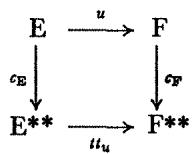
\includegraphics[keepaspectratio]{images/part002_cca49df6.jpg}}

is commutative, as follows immediately from the definitions and formula (15) giving the transpose of a linear mapping.

PROPOSITION 13. If E is a free module (resp. a free module with a finite basis), the canonical mapping \(c_{E}:E \rightarrow E^{**}\) is injective (resp. bijective).

Let \((e_t)_{t \in \mathbb{T}}\) be a basis of \(\mathbf{E}\) and let \((e_t^*)\) be the family of corresponding coordinate forms; by definition, if \(x \in \mathbf{E}\) is such that \(\tilde{x} = 0\) , then \(\langle x, e_t^* \rangle = 0\) for all \(t \in \mathbb{T}\) , in other words all the coordinates of \(x\) are zero, hence \(x = 0\) . Suppose further that \(\mathbf{T}\) is finite; since \(\langle \tilde{e}_t, e_{t'}^* \rangle = \delta_{tt'}\) , \((\tilde{e}_t)\) is the dual basis of \((e_t^*)\) in \(\mathbf{E}^{**}\) and, as \(c_{\mathbf{E}}\) transforms a basis of \(\mathbf{E}\) into a basis of \(\mathbf{E}^{**}\) , \(c_{\mathbf{E}}\) is bijective (§ 1, no. 11, Corollary 3 to Proposition 17). We have moreover proved:

COROLLARY 1. Let E be a free A-module with a finite basis; for every basis \((e_t)\) of E, \((c_{\mathbf{E}}(e_t))\) is the dual basis of the basis \((e_t^*)\) of E* dual to \((e_t)\) .

In this case it is said that \((e_t)\) and \((e_t^*)\) are two dual bases of one another.

COROLLARY 2. If E is a free A-module with a finite basis, every finite basis of \(\mathbf{E}^*\) is the dual basis of a basis of \(\mathbf{E}\) .

It suffices to consider in E** the dual basis of the given basis and canonically to identify E with E**.

COROLLARY 3. Let E, F be two A-modules each with a finite basis, E (resp. F) being canonically identified with its bidual E** (resp. F**). Then, for every linear mapping \(u: \mathbf{E} \to \mathbf{F}\) , \(^{tt}u = u\) .

This follows immediately from the commutativity of diagram (27).

COROLLARY 4. If P is a projective module (resp. a finitely generated projective module) the canonical mapping \(c_{\mathbf{P}}: \mathbf{P} \to \mathbf{P}^{**}\) is injective (resp. bijective).

We shall use the following lemma:

Lemma 1. Let M, N be two supplementary submodules in an A-module E and i: M → E, j: N → E the canonical injections. Then the diagram

\begin{enumerate}
\def\labelenumi{(\arabic{enumi})}
\setcounter{enumi}{27}
\tightlist
\item
\end{enumerate}

\pandocbounded{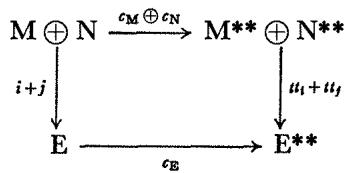
\includegraphics[keepaspectratio]{images/part002_690a791a.jpg}}

is commutative.

By definition, for \(x \in \mathbf{M}\) , \(y \in \mathbf{N}\) , \(z^{*} \in \mathbf{E}^{*}\) ,

\[
\begin{array}{r l} \langle c _ {\mathrm{E}} (i (x) + j (y)), z ^ {*} \rangle & = \langle i (x) + j (y), z ^ {*} \rangle \\ & = \langle i (x), z ^ {*} \rangle + \langle j (y), z ^ {*} \rangle \\ & = \langle x, ^ {t} i (z ^ {*}) \rangle + \langle y, ^ {t} j (z ^ {*}) \rangle \\ & = \langle c _ {\mathrm{M}} (x), ^ {t} i (z ^ {*}) \rangle + \langle c _ {\mathrm{N}} (y), ^ {t} j (z ^ {*}) \rangle \\ & = \langle^ {t t} i (c _ {\mathrm{M}} (x)) + ^ {t t} j (c _ {\mathrm{N}} (y)), z ^ {*} \rangle . \end{array}
\]

This being so, if E is a free module (resp. a free module with a finite basis), \(c_{E}\) is injective (resp. bijective); on the other hand, it follows from no. 6, Proposition 10, that \(^{tt}i \oplus ^{tt}j\) is bijective; the commutativity of diagram (28) then implies that \(c_{M} \oplus c_{N}\) is injective (resp. bijective) and so therefore are \(c_{M}\) and \(c_{N}\) (§ 1, no. 6, Corollary 1 to Proposition 7), whence the corollary, taking account of no. 2, Proposition 4.

\subsection{LINEAR EQUATIONS}

Let E, F be two A-modules. Every equation of the form \(u(x) = y_{0}\) , where \(u: E \to F\) is a given linear mapping, \(y_{0}\) a given element of F and the unknown x is subjected to the condition that it takes its values in E, is called a linear equation; \(y_{0}\) is called the right hand side of the equation; if \(y_{0} = 0\) , the equation is called homogeneous linear.

Every element \(x_{0} \in E\) such that \(u(x_{0}) = y_{0}\) is called a solution of the linear equation \(u(x) = y_{0}\) .†

It is often said, loosely speaking, that a problem is linear if it is equivalent to determining the solutions of a linear equation.

Given a linear equation \(u(x) = y_{0}\) , the equation \(u(x) = 0\) is called the homogeneous linear equation associated with \(u(x) = y_{0}\) .

PROPOSITION 14. If \(x_{0}\) is a solution of the linear equation \(u(x) = y_{0}\) , the set of solutions of this equation is equal to the set of elements \(x_{0} + z\) , where z runs through the set of solutions of the associated homogeneous equation \(u(x) = 0\) .

The relation \(u(x) = y_0\) may be written as \(u(x) = u(x_0)\) , which is equivalent to \(u(x - x_0) = 0\) .

In other words, if the equation \(u(x) = y_{0}\) has at least one solution \(x_{0}\) , the set of its solutions is the set \(x_{0} + u^{-1}(0)\) , obtained by translation from the kernel \(u^{-1}(0)\) of u. Observe that \(u^{-1}(0)\) , being a submodule, is never empty, since it contains 0 (called the zero solution, or trivial solution, of the homogeneous equation \(u(x) = 0\) ).

By virtue of Proposition 14, for a linear equation \(u(x) = y_0\) to have exactly one solution, it is necessary and sufficient that it have at least one solution and that \(u^{-1}(0) = \{0\}\) (in other words, that the associated homogeneous equation have no non-zero solution, or also that \(u\) be injective); in this case, for all \(y \in F\) , the equation \(u(x) = y\) has at most one solution.

PROPOSITION 15. Let \(u\) be a linear mapping of a module \(\mathbf{E}\) into a module \(\mathbf{F}\) . If the equation \(u(x) = y_0\) has at least one solution, \(y_0\) is orthogonal to the kernel of \(^t u\) .

To say that \(u(x) = y_{0}\) admits a solution means that \(y_{0} \in u(\mathbf{E})\) and the proposition follows from no. 5, Corollary to Proposition 8.

Observe that the necessary criterion for the existence of a solution of \(u(x) = y_{0}\) , given by Proposition 15, is sufficient when A is a field (§ 7, no. 6, Proposition 12), but not in general (Exercise 10).

Remarks. (1) Let E be an A-module, \((\mathbf{F}_{i})_{i\in I}\) a family of A-modules and for all \(i\in I\) let \(u_{i}:E\to F_{i}\) be a linear mapping. Every system of linear equations

\[
u _ {i} (x) = y _ {i} \quad (i \in I)\tag{29}
\]

where the \(y_{i} \in \mathbf{F}_{i}\) are given, is equivalent to a single linear equation \(u(x) = y\) , where \(u\) is the mapping \(x \mapsto (u_{i}(x))\) of \(\mathbf{E}\) into \(\mathbf{F} = \prod_{i \in I} \mathbf{F}_{i}\) and \(y = (y_{i})\) . The system (29) is called homogeneous if \(y_{i} = 0\) for all \(i \in I\) .

\begin{enumerate}
\def\labelenumi{(\arabic{enumi})}
\setcounter{enumi}{1}
\tightlist
\item
  Suppose that E admits a basis \((a_{\lambda})_{\lambda \in L}\) ; if we set \(u(a_{\lambda}) = b_{\lambda}\) for all \(\lambda \in L\) , to say that \(x = \sum_{\lambda \in L} \xi_{\lambda} a_{\lambda}\) satisfies the equation \(u(x) = y_0\) is equivalent to saying that the family (of finite support) \((\xi_{\lambda})_{\lambda \in L}\) of elements of A satisfies the relation
\end{enumerate}

\[
\sum_ {\lambda \in L} \xi_ {\lambda} b _ {\lambda} = y _ {0}.\tag{30}
\]

Conversely, looking for families \((\xi_{\lambda})_{\lambda \in L}\) of elements of A of finite support satisfying (30), is equivalent to solving the linear equation \(u(x) = y_0\) , where \(u\) is the unique linear mapping of E into F such that \(u(a_{\lambda}) = b_{\lambda}\) for all \(\lambda \in L\) (§ 1, no. 11, Corollary 3 to Proposition 17).

\begin{enumerate}
\def\labelenumi{(\arabic{enumi})}
\setcounter{enumi}{2}
\tightlist
\item
  A linear equation \(u(x) = y_0\) is called scalar when \(F = A_s\) and therefore \(u\) is a linear form on \(E\) and \(y_0\) a scalar. If \(E\) admits a basis \((a_\lambda)_{\lambda \in L}\) , it follows from Remark (2) that such an equation may also be written as
\end{enumerate}

\[
\sum_ {\lambda \in L} \xi_ {\lambda} \alpha_ {\lambda} = y _ {0} \in A\tag{31}
\]

where the family of scalars \((\alpha_{\lambda})\) is arbitrary and where it is understood that the family \((\xi_{\lambda})\) must have finite support. In general, by the solution (in A) of a system of scalar linear equations

\[
\sum_ {\lambda \in L} \xi_ {\lambda} \alpha_ {\lambda i} = \eta_ {i} \quad (i \in I)\tag{32}
\]

where \(\alpha_{\lambda i} \in A\) and \(\eta_i \in A\) , is understood a family \((\xi_\lambda)_{\lambda \in L}\) of elements of \(A\) of finite support and satisfying (32); the \(\alpha_{\lambda i}\) are called the coefficients of the system of equations and the \(\eta_i\) the right hand sides. The solution of such a system is equivalent to that of the equation \(u(x) = y\) , where \(y = (\eta_i)\) and \(u: A_s^{(L)} \to A_s^I\) is the linear mapping

\[
\left(\xi_ {\lambda}\right) \mapsto \left(\sum_ {\lambda \in L} \xi_ {\lambda} \alpha_ {\lambda i}\right).
\]

\begin{enumerate}
\def\labelenumi{(\arabic{enumi})}
\setcounter{enumi}{3}
\tightlist
\item
  A linear system (32) is also called a system of left scalar linear equations when it is necessary to avoid confusion. A system of equations
\end{enumerate}

\[
\sum_ {\lambda \in L} \alpha_ {\lambda i} \xi_ {\lambda} = \eta_ {i} \quad (i \in I)\tag{33}
\]

is likewise called a system of right scalar linear equations; such a system can immediately be transformed into a system (32) by considering the \(\xi_{\lambda}, \eta_{i}\) and \(\alpha_{\lambda i}\) as belonging to the opposite ring A \(^{0}\) to A.

\section{TENSOR PRODUCTS}

\subsection{TENSOR PRODUCT OF TWO MODULES}

Let \(G_{1}, G_{2}\) be two Z-modules; a mapping u of the set \(G = G_{1} \times G_{2}\) into a Z-module is called biadditive (or Z-bilinear) if \(u(x_{1}, x_{2})\) is ``additive with respect to \(x_{1}\) and with respect to \(x_{2}\) ''; to be precise, this means that, for \(x_{1}, y_{1}\) in \(G_{1}, x_{2}, y_{2}\) in \(G_{2}\) ,

\[
\begin{array}{l} u (x _ {1} + y _ {1}, x _ {2}) = u (x _ {1}, x _ {2}) + u (y _ {1}, x _ {2}) \\ u (x _ {1}, x _ {2} + y _ {2}) = u (x _ {1}, x _ {2}) + u (x _ {1}, y _ {2}). \end{array}
\]

Note that this implies in particular that \(u(0, x_2) = u(x_1, 0) = 0\) for all \(x_1 \in \mathbf{G}_1, x_2 \in \mathbf{G}_2\) .

Let A be a ring, E a right A-module and F a left A-module. We are going to consider the universal mapping problem (Set Theory, IV, § 3, no. 1) where \(\Sigma\) is the species of Z-module structure (the morphisms then being Z-linear mappings, in other words, additive group homomorphisms) and the \(\alpha\) -mappings are the mappings \(f\) of E \(\times\) F into a Z-module G which are Z-bilinear and further satisfy, for all \(x \in \mathbf{E}\) , \(y \in \mathbf{F}\) and \(\lambda \in \mathbf{A}\)

\[
f (x \lambda , y) = f (x, \lambda y).\tag{1}
\]

We show that this problem admits a solution. For this we consider the Z-module \(C = \mathbf{Z}^{(E \times F)}\) of formal linear combinations of the elements of \(E \times F\) with coefficients in Z (§ 1, no. 11), a basis of which can be considered to consist of the ordered pairs \((x, y)\) , where \(x \in E\) and \(y \in F\) . Let D be the sub-Z-module of C generated by the elements of one of the following types:

\[
\left\{ \begin{array}{l} (x _ {1} + x _ {2}, y) - (x _ {1}, y) - (x _ {2}, y) \\ (x, y _ {1} + y _ {2}) - (x, y _ {1}) - (x, y _ {2}) \\ (x \lambda , y) - (x, \lambda y) \end{array} \right.\tag{2}
\]

where \(x, x_{1}, x_{2}\) are in E, \(y, y_{1}, y_{2}\) are in F and \(\lambda\) is in A.

DEFINITION 1. The tensor product of the right A-module E and the left A-module F, denoted by \(\mathbf{E} \otimes_{\mathbf{A}} \mathbf{F}\) or \(\mathbf{E} \otimes_{\mathbf{A}} \mathbf{F}\) (or simply \(\mathbf{E} \otimes \mathbf{F}\) if no confusion is to be feared) is the quotient \(\mathbf{Z}\) -module C/D (the quotient of the \(\mathbf{Z}\) -module C of formal linear combinations of elements of \(\mathbf{E} \times \mathbf{F}\) with coefficients in \(\mathbf{Z}\) , by the submodule \(\mathbf{D}\) generated by the elements of one of the types (2)). For \(x \in \mathbf{E}\) and \(y \in \mathbf{F}\) , the element of \(\mathbf{E} \otimes_{\mathbf{A}} \mathbf{F}\) which is the canonical image of the element \((x, y)\) of \(\mathbf{C} = \mathbf{Z}^{(\mathbf{E} \times \mathbf{F})}\) is denoted by \(x \otimes y\) and called the tensor product of \(x\) and \(y\) .

The mapping \((x,y)\mapsto x\otimes y\) of \(\mathbf{E}\times \mathbf{F}\) into \(\mathbf{E}\otimes_{\mathbf{A}}\mathbf{F}\) is called canonical. It is a Z-bilinear mapping which satisfies conditions (1).

We show that the tensor product \(E \otimes_{A} F\) and the above canonical mapping form a solution of the universal mapping problem posed earlier. To be precise:

PROPOSITION 1. (a) Let \(g\) be a \(\mathbf{Z}\) -linear mapping of \(\mathbf{E} \otimes_{\mathbf{A}} \mathbf{F}\) into a \(\mathbf{Z}\) -module \(\mathbf{G}\) . The mapping \((x, y) \mapsto f(x, y) = g(x \otimes y)\) of \(\mathbf{E} \times \mathbf{F}\) into \(\mathbf{G}\) is \(\mathbf{Z}\) -bilinear and satisfies conditions (1).

\begin{enumerate}
\def\labelenumi{(\alph{enumi})}
\setcounter{enumi}{1}
\tightlist
\item
  Conversely, let \(f\) be a \(\mathbf{Z}\) -bilinear mapping of \(\mathbf{E} \times \mathbf{F}\) into a \(\mathbf{Z}\) -module \(\mathbf{G}\) satisfying conditions (1). Then there exists one and only one \(\mathbf{Z}\) -linear mapping \(g\) of \(\mathbf{E} \otimes_{\mathbf{A}} \mathbf{F}\) into \(\mathbf{G}\) such that \(f(x,y) = g(x \otimes y)\) for \(x \in \mathbf{E}, y \in \mathbf{F}\) .
\end{enumerate}

If \(\phi\) denotes the canonical mapping of \(\mathbf{E} \times \mathbf{F}\) into \(\mathbf{E} \otimes_{\mathbf{A}} \mathbf{F}\) , then \(f = g \circ \phi\) ; whence (a). To show (b), we note that, in the notation of Definition 1, \(f\) extends to a \(\mathbf{Z}\) -linear mapping \(\bar{f}\) of \(\mathbf{C}\) into \(\mathbf{G}\) ( \(\S 1\) , no. 11, Proposition 17). By virtue of relations (1), \(\bar{f}\) is zero for all the elements of \(\mathbf{C}\) of one of the types (2) and hence on \(\mathbf{D}\) . There therefore exists a \(\mathbf{Z}\) -linear mapping \(g\) of \(\mathbf{C} / \mathbf{D} = \mathbf{E} \otimes_{\mathbf{A}} \mathbf{F}\) into \(\mathbf{G}\) such that \(\bar{f} = g \circ \psi\) , where \(\psi: \mathbf{C} \to \mathbf{C} / \mathbf{D}\) is the canonical homomorphism ( \(\S 1\) , no. 8, Remark). The uniqueness of \(g\) is immediate since \(\mathbf{E} \otimes_{\mathbf{A}} \mathbf{F}\) is generated, as a \(\mathbf{Z}\) -module, by the elements of the form \(x \otimes y\) .

Proposition 1 defines a canonical isomorphism of the Z-module of Z-bilinear mappings f of E × F into G, satisfying conditions (1), onto the Z-module Hom \(_{Z}\) (E ⊗A F, G).

When A = Z, conditions (1) are automatically satisfied for every Z-bilinear mapping f and the submodule D of C is already generated by the elements of the first two types in (2).

If now we return to the general case and \(E'\) and \(F'\) denote the underlying Z-modules of E and F respectively, the above remark and Definition 1 show immediately that the Z-module \(E \otimes_{A} F\) can be canonically identified with the quotient of the Z-module \(E' \otimes_{Z} F'\) by the sub-Z-module generated by the elements of the form \((x\lambda) \otimes y - x \otimes (\lambda y)\) , where x runs through E, y runs through F and \(\lambda\) runs through A.

COROLLARY 1. Let H be a Z-module and \(h:E \times F \rightarrow H\) a Z-bilinear mapping satisfying conditions (1) and such that H is generated by \(h(E \times F)\) . Suppose that for every Z-module G and every Z-bilinear mapping f of \(E \times F\) into G satisfying (1)

there exists a Z-linear mapping \(g:H \to G\) such that \(f = g \circ h\) . Then, if \(\phi\) denotes the canonical mapping of \(E \times F\) into \(E \otimes_{A} F\) , there exists one and only one isomorphism \(\theta\) of \(E \otimes_{A} F\) onto H such that \(h = \theta \circ \phi\) .

The hypothesis that \(h(\mathbf{E} \times \mathbf{F})\) generates H implies the uniqueness of g; the corollary is then just the general uniqueness property of a solution of a universal mapping problem (Set Theory, IV, § 3, no. 1).

COROLLARY 2. Let \(\mathbf{E}^0\) (resp. \(\mathbf{F}^0\) ) denote the module \(\mathbf{E}\) (resp. \(\mathbf{F}\) ) considered as a left (resp. right) module over the opposite ring \(\mathbf{A}^0\) ; then there exists one and only one \(\mathbf{Z}\) -module isomorphism \(\sigma: \mathbf{E} \otimes_{\mathbf{A}} \mathbf{F} \to \mathbf{F}^0 \otimes_{\mathbf{A}^0} \mathbf{E}^0\) such that \(\sigma(x \otimes y) = y \otimes x\) for \(x \in \mathbf{E}\) and \(y \in \mathbf{F}\) (``commutativity'' of tensor products).

By definition of the \(A^{0}\) -module structures on \(E^{0}\) and \(F^{0}\) , the mapping \((x,y)\mapsto y\otimes x\) of \(E\times F\) into \(F^{0}\otimes_{A^{0}}E^{0}\) is Z-bilinear and satisfies conditions (1), whence the existence and uniqueness of the Z-linear mapping \(\sigma\) . Similarly a Z-linear mapping \(\tau:F^{0}\otimes_{A^{0}}E^{0}\to E\otimes_{A}F\) is defined such that \(\tau(y\otimes x)=x\otimes y\) and clearly \(\sigma\) and \(\tau\) are inverse isomorphisms.

Remark. The tensor product of non-zero modules may be zero: for example, taking the two Z-modules E = Z/2Z and F = Z/3Z, 2x = 0 and 3y = 0 for all \(x \in E\) and \(y \in F\) ; therefore, in E \(\otimes_{\mathbf{Z}} F\) ,

\[
x \otimes y = 3 (x \otimes y) - 2 (x \otimes y) = x \otimes (3 y) - (2 x) \otimes y = 0
\]

for all \(x\) and \(y\) (cf.~no. 6, Corollary 4 to Proposition 6).

\subsection{TENSOR PRODUCT OF TWO LINEAR MAPPINGS}

Let A be a ring, E, E' two right A-modules, F, F' two left A-modules and \(u: E \rightarrow E'\) and \(v: F \rightarrow F'\) two A-linear mappings. It is easily verified that the mapping

\[
(x, y) \mapsto u (x) \otimes v (y)
\]

of \(\mathbf{E} \times \mathbf{F}\) into \(\mathbf{E}' \otimes_{\mathbf{A}} \mathbf{F}'\) is \(\mathbf{Z}\) -bilinear and satisfies conditions (1) of no. 1. By Proposition 1 of no. 1 there thus exists one and only one \(\mathbf{Z}\) -linear mapping \(w: \mathbf{E} \otimes_{\mathbf{A}} \mathbf{F} \to \mathbf{E}' \otimes_{\mathbf{A}} \mathbf{F}'\) such that

\[
w (x \otimes y) = u (x) \otimes v (y)\tag{3}
\]

for \(x \in \mathbf{E}\) , \(y \in \mathbf{F}\) . This mapping is denoted by \(u \otimes v\) (when no confusion can arise) and is called the tensor product of the linear mappings \(u\) and \(v\) .

It follows immediately from (3) that \((u, v) \mapsto u \otimes v\) is a Z-bilinear mapping called canonical

\[
\operatorname{Hom} _ {\mathbf {A}} (\mathrm{E}, \mathrm{E} ^ {\prime}) \times \operatorname{Hom} _ {\mathbf {A}} (\mathrm{F}, \mathrm{F} ^ {\prime}) \rightarrow \operatorname{Hom} _ {\mathbf {Z}} (\mathrm{E} \otimes_ {\mathbf {A}} \mathrm{F}, \mathrm{E} ^ {\prime} \otimes_ {\mathbf {A}} \mathrm{F} ^ {\prime}).
\]

There corresponds to it by Proposition 1 of no. 1 a \(\mathbf{Z}\) -linear mapping called canonical

\[
\operatorname{Hom} _ {\mathbf {A}} (\mathrm{E}, \mathrm{E} ^ {\prime}) \otimes_ {\mathbf {Z}} \operatorname{Hom} _ {\mathbf {A}} (\mathrm{F}, \mathrm{F} ^ {\prime}) \rightarrow \operatorname{Hom} _ {\mathbf {Z}} (\mathrm{E} \otimes_ {\mathbf {A}} \mathrm{F}, \mathrm{E} ^ {\prime} \otimes_ {\mathbf {A}} \mathrm{F} ^ {\prime})\tag{4}
\]

which associates with every element \(u \otimes v\) of the tensor product the linear mapping \(u \otimes v: \mathbf{E} \otimes_{\mathbf{A}} \mathbf{F} \to \mathbf{E}' \otimes_{\mathbf{A}} \mathbf{F}'\) . Note that the canonical mapping (4) is not necessarily injective nor surjective. The notation \(u \otimes v\) can therefore lead to confusion and it will be necessary for the context to indicate whether it denotes an element of the tensor product or a linear mapping.

Further, let \(\mathbf{E}''\) be a right A-module, \(\mathbf{F}''\) a left A-module and \(u':\mathbf{E}'\to\mathbf{E}''\) , \(v':\mathbf{F}'\to\mathbf{F}''\) A-linear mappings; it follows from (3) that

\[
\left(u ^ {\prime} \circ u\right) \otimes \left(v ^ {\prime} \circ v\right) = \left(u ^ {\prime} \otimes v ^ {\prime}\right) \circ (u \otimes v).\tag{5}
\]

\subsection{CHANGE OF RING}

PROPOSITION 2. Let A, B be two rings, \(\rho: \mathbf{B} \to \mathbf{A}\) a ring homomorphism and E (resp. F) a right (resp. left) A-module. Then there exists one and only one Z-linear mapping

\[
\phi : \rho_ {*} (\mathbf {E}) \otimes_ {\mathbf {B}} \rho_ {*} (\mathbf {F}) \rightarrow \mathbf {E} \otimes_ {\mathbf {A}} \mathbf {F}\tag{6}
\]

such that, for all \(x \in \mathbf{E}\) and \(y \in \mathbf{F}\) , the image under \(\phi\) of the element \(x \otimes y\) of \(\rho_{*}(\mathbf{E}) \otimes_{\mathbf{B}} \rho_{*}(\mathbf{F})\) is the element \(x \otimes y\) of \(\mathbf{E} \otimes_{\mathbf{A}} \mathbf{F}\) ; this \(\mathbf{Z}\) -linear mapping is surjective.

We consider the mapping \((x,y)\mapsto x\otimes y\) of \(\rho_{\star}(E)\times \rho_{*}(F)\) into \(E\otimes_A F\) ; it is Z-bilinear and, for all \(\beta \in B\) , by definition \((x\rho (\beta))\otimes y = x\otimes (\rho (\beta)y)\) , hence conditions (1) of no. 1 hold, whence the existence and uniqueness of \(\phi\) (no. 1, Proposition 1). The latter assertion follows from the fact that the elements \(x\otimes y\) generate the Z-module \(E\otimes_A F\) .

The mapping (6) is called canonical.

COROLLARY. Let \(\mathfrak{a}\) be a two-sided ideal of A such that \(\mathfrak{a}\) is contained in the annihilator of E and in the annihilator of F, so that E (resp. F) has a canonical left (resp. right) \((A/\mathfrak{a})\)-module structure (§ 1, no. 12). Then the canonical homomorphism (6)

\[
\phi : \mathbf {E} \otimes_ {\mathbf {A}} \mathbf {F} \rightarrow \mathbf {E} \otimes_ {\mathbf {A} / \mathfrak {a}} \mathbf {F}
\]

corresponding to the canonical homomorphism \(\rho: \mathbf{A} \to \mathbf{A} / \mathfrak{a}\) is the identity.

For all \(\bar{\alpha} \in \mathbf{A} / \mathfrak{a}\) , all \(x \in \mathbf{E}\) and all \(y \in \mathbf{F}\) , \(x\bar{\alpha} = x\alpha\) (resp. \(\bar{\alpha}y = \alpha y\) ) for all \(\alpha\) such that \(\rho(\alpha) = \bar{\alpha}\) . If \(\mathbf{C} = \mathbf{Z}^{(\mathbb{E} \times \mathbb{F})}\) , the submodule of \(\mathbf{C}\) generated by the elements \((x\alpha, y) - (x, \alpha y)\) is then equal to the submodule generated by the elements \((x\bar{\alpha}, y) - (x, \bar{\alpha}y)\) .

With the hypotheses and notation of Proposition 2, let \(\mathbf{E}'\) be a right B-module, \(\mathbf{F}'\) a left B-module and consider two semi-linear mappings \(u: \mathbf{E}' \to \mathbf{E}\) , \(v: \mathrm{F}' \to \mathrm{F}\) relative to the homomorphism \(\rho: \mathrm{B} \to \mathrm{A}\) ; \(u\) (resp. \(v\) ) can be considered as a B-linear mapping \(\mathrm{E}' \to \rho_*(\mathrm{E})\) (resp. \(\mathrm{F}' \to \rho_*(\mathrm{F})\) ), whence a Z-linear mapping \(w: \mathrm{E}' \otimes_{\mathrm{B}} \mathrm{F}' \to \rho_*(\mathrm{E}) \otimes_{\mathrm{B}} \rho_*(\mathrm{F})\) such that \(w(x' \otimes y') = u(x') \otimes v(y')\) for \(x' \in \mathrm{E}', y' \in \mathrm{F}'\) ; composing the canonical mapping (6) with this mapping, a Z-linear mapping \(w': \mathrm{E}' \otimes_{\mathrm{B}} \mathrm{F}' \to \mathrm{E} \otimes_{\mathrm{A}} \mathrm{F}\) is hence obtained such that \(w'(x' \otimes y') = u(x') \otimes v(y')\) for \(x' \in \mathrm{E}', y' \in \mathrm{F}'\) ; this is the mapping which will normally be denoted by \(u \otimes v\) if no confusion can arise. Clearly \((u, v) \mapsto u \otimes v\) is a Z-bilinear mapping

\[
\operatorname{Hom} _ {\mathbf {B}} \left(\mathrm{E} ^ {\prime}, \rho_ {*} (\mathrm{E})\right) \times \operatorname{Hom} _ {\mathbf {B}} \left(\mathrm{F} ^ {\prime}, \rho_ {*} (\mathrm{F})\right)\rightarrow \operatorname{Hom} _ {\mathbf {Z}} \left(\mathrm{E} ^ {\prime} \otimes_ {\mathbf {B}} \mathrm{F} ^ {\prime}, \mathrm{E} \otimes_ {\mathbf {A}} \mathrm{F}\right).
\]

Moreover, if C is a third ring, \(\sigma: \mathrm{C} \to \mathrm{B}\) a homomorphism, \(\mathrm{E}''\) a right C-module, \(\mathrm{F}''\) a left C-module, \(u': \mathrm{E}'' \to \mathrm{E}'\) and \(v': \mathrm{F}'' \to \mathrm{F}'\) semi-linear mappings relative to \(\sigma\) , then

\[
(u \circ u ^ {\prime}) \otimes (v \circ v ^ {\prime}) = (u \otimes v) \circ (u ^ {\prime} \otimes v ^ {\prime}).
\]

\subsection{OPERATORS ON A TENSOR PRODUCT; TENSOR PRODUCTS AS MULTI-MODULES}

With the hypotheses and notation of no. 1, for every endomorphism \(u\) (resp. \(v\) ) of the A-module \(E\) (resp. \(F\) ), \(u \otimes l_F\) (resp. \(l_E \otimes v\) ) is an endomorphism of the \(Z\) -module \(E \otimes_A F\) ; it follows immediately from (5) (no. 2) that the mapping \(u \mapsto u \otimes l_F\) (resp. \(v \mapsto l_E \otimes v\) ) is a ring homomorphism

\[
\operatorname{End} _ {\mathbf {A}} (\mathbf {E}) \rightarrow \operatorname{End} _ {\mathbf {Z}} (\mathbf {E} \otimes_ {\mathbf {A}} \mathbf {F})
\]

(resp. \(\operatorname{End}_{\mathbf{A}}(\mathbf{F}) \to \operatorname{End}_{\mathbf{Z}}(\mathbf{E} \otimes_{\mathbf{A}} \mathbf{F}))\) ; moreover,

\[
(u \otimes \mathrm{l} _ {\mathrm{F}}) \circ (\mathrm{l} _ {\mathrm{E}} \otimes v) = (\mathrm{l} _ {\mathrm{E}} \otimes v) \circ (u \otimes \mathrm{l} _ {\mathrm{F}}) = u \otimes v\tag{7}
\]

and therefore (§ 1, no. 14) E ⊗\_A F has a canonical left bimodule structure with respect to the rings End\_A(E) and End\_A(F).

This being so, suppose given on E a \(((\mathbf{B}_i^{\prime});\mathbf{A},(\mathbf{C}_j^{\prime}))\) -multimodule structure and on F a \((\mathbf{A},(\mathbf{B}_h^{\prime});(\mathbf{C}_k^{\prime}))\) -multimodule structure (§ 1, no. 14); it amounts to the same to say that ring homomorphisms \(\mathrm{B}_i^\prime \to \mathrm{End}_{\mathbf{A}}(\mathbf{E})\) , \(\mathrm{C}_j^{\prime 0} \to \mathrm{End}_{\mathbf{A}}(\mathbf{E})\) are given with pairwise permutable images, and ring homomorphisms \(\mathrm{B}_h^{\prime \prime} \to \mathrm{End}_{\mathbf{A}}(\mathbf{F})\) , \(\mathrm{C}_k^{\prime \prime 0} \to \mathrm{End}_{\mathbf{A}}(\mathbf{F})\) with pairwise permutable images. If these homomorphisms are composed respectively with the canonical homomorphisms \(\mathrm{End}_{\mathbf{A}}(\mathbf{E}) \to \mathrm{End}_{\mathbf{Z}}(\mathbf{E} \otimes_{\mathbf{A}} \mathbf{F})\) and \(\mathrm{End}_{\mathbf{A}}(\mathbf{F}) \to \mathrm{End}_{\mathbf{Z}}(\mathbf{E} \otimes_{\mathbf{A}} \mathbf{F})\) defined above, it is seen (taking account of (7)) that ring homomorphisms

\[
\mathrm{B} _ {i} ^ {\prime} \rightarrow \operatorname{End} _ {\mathbf {Z}} (\mathrm{E} \otimes_ {\mathrm{A}} \mathrm{F}), \quad \mathrm{C} _ {j} ^ {\prime 0} \rightarrow \operatorname{End} _ {\mathbf {Z}} (\mathrm{E} \otimes_ {\mathrm{A}} \mathrm{F})
\]

\[
\mathrm{B} _ {h} ^ {\prime \prime} \rightarrow \operatorname{End} _ {\mathbf {Z}} (\mathrm{E} \otimes_ {\mathrm{A}} \mathrm{F}), \quad \mathrm{C} _ {k} ^ {\prime \prime 0} \rightarrow \operatorname{End} _ {\mathbf {Z}} (\mathrm{E} \otimes_ {\mathrm{A}} \mathrm{F})
\]

are defined with pairwise permutable images; in other words, there has been defined on \(\mathbf{E} \otimes_{\mathbf{A}} \mathbf{F}\) a \(((\mathbf{B}_i'), (\mathbf{B}_h''); (\mathbf{C}_j'), (\mathbf{C}_k'')\) -multimodule structure; it is this multimodule which is also called the tensor product (relative to A) of the \(((\mathbf{B}_i^{\prime});\mathbf{A},(\mathbf{C}_j^{\prime}))\) -multimodule E and the \((\mathbf{A},(\mathbf{B}_h^{\prime\prime});(\mathbf{C}_k^{\prime\prime}))\) -multimodule F. This multi-module is the solution of a universal mapping problem analogous to that considered in no. 1; to be precise:

PROPOSITION 3. Let G be a \(((\mathbf{B}_i'), (\mathbf{B}_h''); (\mathbf{C}_j'), (\mathbf{C}_k''))-multimodule.\)

\begin{enumerate}
\def\labelenumi{(\alph{enumi})}
\tightlist
\item
  Let \(g\) be a linear mapping of the multimodule \(\mathbf{E} \otimes_{\mathbf{A}} \mathbf{F}\) into \(\mathbf{G}\) . The mapping \(f: (x, y) \mapsto g(x \otimes y)\) of \(\mathbf{E} \times \mathbf{F}\) into \(\mathbf{G}\) is \(\mathbf{Z}\) -bilinear and satisfies relations (1) of no. 1 and the conditions
\end{enumerate}

\[
\left\{ \begin{array}{l l} f (\mu_ {i} ^ {\prime} x, y) = \mu_ {i} ^ {\prime} f (x, y), & f (x \nu_ {j} ^ {\prime}, y) = f (x, y) \nu_ {j} ^ {\prime} \\ f (x, \mu_ {h} ^ {\prime \prime} y) = \mu_ {h} ^ {\prime \prime} f (x, y), & f (x, y \nu_ {k} ^ {\prime \prime}) = f (x, y) \nu_ {k} ^ {\prime \prime} \end{array} \right.\tag{8}
\]

for all \(x \in \mathbf{E}, y \in \mathbf{F}\) , \(\mu_i' \in \mathbf{B}_i'\) , \(\nu_j' \in \mathbf{C}_j'\) , \(\mu_h'' \in \mathbf{B}_h''\) , \(\nu_k'' \in \mathbf{C}_{k}''\) , \(i, j, h, k\) arbitrary.

\begin{enumerate}
\def\labelenumi{(\alph{enumi})}
\setcounter{enumi}{1}
\tightlist
\item
  Conversely, let \(f\) be a \(\mathbf{Z}\) -bilinear mapping of \(\mathbf{E} \times \mathbf{F}\) into \(\mathbf{G}\) satisfying conditions (1) (no. 1) and (8). Then there exists one and only one linear mapping \(g\) of the multimodule \(\mathbf{E} \otimes_{\mathbf{A}} \mathbf{F}\) into the multimodule \(\mathbf{G}\) such that \(f(x, y) = g(x \otimes y)\) for \(x \in \mathbf{E}, y \in \mathbf{F}\) .
\end{enumerate}

Assertion (a) follows immediately from the definition of the multimodule structure on \(\mathbf{E} \otimes_{\mathbf{A}} \mathbf{F}\) , since for example \((x \otimes y)\nu_j' = (x\nu_j') \otimes y\) . To prove (b), we note first that Proposition 1 of no. 1 gives the existence and uniqueness of a \(\mathbf{Z}\) -linear mapping \(g\) such that \(g(x \otimes y) = f(x, y)\) for \(x \in \mathbf{E}\) , \(y \in \mathbf{F}\) ; all that is needed is to verify that \(g\) is linear for the multimodule structures. As the elements \(x \otimes y\) generate the \(\mathbf{Z}\) -module \(\mathbf{E} \otimes_{\mathbf{A}} \mathbf{F}\) , it suffices to verify the relations \(g(\mu'(x \otimes y)) = \mu_i' g(x \otimes y)\) and their analogues; but this follows immediately from the formula \(g(x \otimes y) = f(x, y)\) and relations (8).

SCHOLIUM. An element of \(\mathbf{E} \otimes_{\mathbf{A}} \mathbf{F}\) may in general be written in several ways in the form \(\sum_{i} (x_i \otimes y_i)\) , where \(x_i \in \mathbf{E}\) and \(y_i \in \mathbf{F}\) ; but to define a linear mapping \(g\) of the multimodule \(\mathbf{E} \otimes_{\mathbf{A}} \mathbf{F}\) into a multimodule \(\mathbf{G}\) , there is no need to verify that, if \(\sum_{i} (x_i \otimes y_i) = \sum_{j} (x_j' \otimes y_j')\) , then \(\sum_{i} g(x_i \otimes y_i) = \sum_{j} g(x_j' \otimes y_j')\) ; it suffices to be given \(g(x \otimes y)\) for \(x \in \mathbf{E}\) and \(y \in \mathbf{F}\) and to verify that \((x, y) \mapsto g(x \otimes y)\) is \(\mathbf{Z}\) -bilinear and satisfies conditions (1) (no. 1) and (8).

Let \(\mathbf{E}'\) be a \(((\mathbf{B}_i'),\mathbf{A},(\mathbf{C}_j')\) -multimodule, \(\mathbf{F}'\) an \((\mathbf{A},(\mathbf{B}_h'');(\mathbf{C}_k'')\) -multimodule and \(u:\mathbf{E}\to \mathbf{E}',v:\mathbf{F}\to \mathbf{F}'\) linear mappings of multimodules; it follows immediately from the definitions (no. 2) that \(u\otimes v\) is a linear mapping of the multimodule \(\mathbf{E}\otimes_{\mathbf{A}}\mathbf{F}\) into the multimodule \(\mathbf{E}'\otimes_{\mathbf{A}}\mathbf{F}'\) .

With E always denoting a right A-module, let \(_{s}A_{d}\) denote the ring A considered as an (A, A)-bimodule ( \(\S\) 1, no. 14, Example 1); by the above, the tensor product \(\mathbf{E} \otimes_{\mathbf{A}} (\mathbf{s}\mathbf{A}_{d})\) has a canonical right A-module structure such that \((x \otimes \lambda)\mu = x \otimes (\lambda\mu)\) for \(x \in E\) , \(\lambda \in A\) , \(\mu \in A\) . The mapping \((x, \lambda) \mapsto x\lambda\) of \(\mathbf{E} \times (\mathbf{s}\mathbf{A}_{d})\) into E is Z-bilinear and satisfies conditions (1) (no. 1) and (8)

(where, in the latter, the \(\mathbf{B}_i'\) , \(\mathbf{C}_j'\) and \(\mathbf{B}_h''\) are absent and the family \((\mathbf{C}_k'')\) reduces to \(\mathbf{A}\) ); hence (Proposition 3), there exists an A-linear mapping \(g\) (called canonical) of \(\mathbf{E} \otimes_{\mathbf{A}} (s\mathbf{A}_d)\) into \(\mathbf{E}\) such that \(g(x \otimes \lambda) = x\lambda\) for \(x \in \mathbf{E}\) , \(\lambda \in \mathbf{A}\) .

PROPOSITION 4. If E is a right A-module, the mapping \(h: x \mapsto x \otimes 1\) of E into \(\mathbf{E} \otimes_{\mathbf{A}} (s\mathbf{A}_d)\) is a right A-module isomorphism, whose inverse isomorphism \(g\) is such that \(g(x \otimes \lambda) = x\lambda\) for \(x \in \mathbf{E}, \lambda \in \mathbf{A}\) .

If \(g\) is the canonical mapping, \(g \circ h\) is the identity mapping \(1_{\mathbf{E}}\) and \(h \circ g\) coincides with the identity mapping of \(\mathbf{E} \otimes_{\mathbf{A}} (s\mathbf{A}_d)\) onto itself for elements of the form \(x \otimes y\) , which generate the latter \(\mathbf{Z}\) -module; hence the conclusion.

We shall normally write \(E \otimes_{A} A\) instead of \(E \otimes_{A} (s A_{d})\) and shall often identify \(E \otimes_{A} A\) with E by means of the above canonical isomorphisms. Observe that, if E also has a (left or right) B-module structure which is compatible with its right A-module structure, g and h are also isomorphisms for the B-module structures on E and \(E \otimes_{A} A\) (and hence multimodule isomorphisms).

Now let F be a left A-module; \((sA_{d}) \otimes_{A} F\) (also denoted by A \(\otimes_{A} F\) ) then has a canonical left A-module structure and as in Proposition 4 a canonical isomorphism is defined of A \(\otimes_{A} F\) onto F mapping \(\lambda \otimes x\) to \(\lambda x\) , and its inverse isomorphism is \(x \mapsto 1 \otimes x\) .

In particular there exists a canonical isomorphism of the (A, A)-bimodule \((_{s}\mathbf{A}_{d})\otimes_{\mathbf{A}}(_{s}\mathbf{A}_{d})\) onto \({}_{s}\mathbf{A}_{d}\) which maps \(\lambda \otimes \mu\) to \(\lambda \mu\) .

\subsection{TENSOR PRODUCT OF TWO MODULES OVER A COMMUTATIVE RING}

Let C be a commutative ring; for every C-module E, the module structure on E is compatible with itself (§ 1, no. 14). If E and F are two C-modules, the considerations of no. 4 then allow us to define two C-module structures on the tensor product E ⊗c F, respectively such that γ(x ⊗ y) = (γx) ⊗ y and such that γ(x ⊗ y) = x ⊗ (γy); but as, by Definition 1 of no. 1, in this case (γx) ⊗ y = x ⊗ (γy), these two structures are the same. Henceforth when we speak of E ⊗c F as a C-module, we shall mean with the structure thus defined, unless otherwise stated. The canonical isomorphism.

\[
\sigma : \mathbf {F} \otimes_ {\mathbf {c}} \mathbf {E} \rightarrow \mathbf {E} \otimes_ {\mathbf {c}} \mathbf {F}
\]

(no. 1, Corollary 2 to Proposition 1) is then a C-module isomorphism.

It follows from this definition that, if \((a_{\lambda})_{\lambda\in\mathbb{L}}\) (resp. \((b_{\mu})_{\mu\in\mathbb{M}}\) ) is a generating system of the C-module E (resp. F), \((a_{\lambda}\otimes b_{\mu})\) is a generating system of the C-module \(E\otimes_{C}F\) ; in particular, if E and F are finitely generated C-modules, so is \(E\otimes_{C}F\) .

For every C-module G, the Z-bilinear mappings \(f\) of \(\mathbf{E} \times \mathbf{F}\) into \(\mathbf{G}\) for which

\[
f (\gamma x, y) = f (x, \gamma y) = \gamma f (x, y) \quad \text { for } x \in \mathbf {E}, y \in \mathbf {F}, \gamma \in \mathbf {C}\tag{9}
\]

are then called C-bilinear and form a C-module denoted by \(\mathcal{L}_2(\mathrm{E},\mathrm{F};\mathrm{G})\) ; Proposition 3 (no. 4) defines a canonical C-module isomorphism (cf.~§1, no. 14, Remark 1).

\[
\mathcal {L} _ {2} (\mathrm{E}, \mathrm{F}; \mathrm{G}) \rightarrow \operatorname{Hom} _ {\mathbf {c}} (\mathrm{E} \otimes_ {\mathbf {c}} \mathrm{F}, \mathrm{G}).\tag{10}
\]

Let \(E'\) , \(F'\) be two C-modules and \(u: E \to E'\) , \(v: F \to F'\) two C-linear mappings; then (no. 4) \(u \otimes v\) is a C-linear mapping of \(E \otimes_{\mathbb{C}} F\) into \(E' \otimes_{\mathbb{C}} F'\) . Further, it is immediate that \((u, v) \mapsto u \otimes v\) is a C-bilinear mapping of \(\operatorname{Hom}_{\mathbb{C}}(\mathbf{E}, \mathbf{E}') \times \operatorname{Hom}_{\mathbb{C}}(\mathbf{F}, \mathbf{F}')\) into \(\operatorname{Hom}_{\mathbb{C}}(\mathbf{E} \otimes_{\mathbb{C}} \mathbf{F}, \mathbf{E}' \otimes_{\mathbb{C}} \mathbf{F}')\) ; hence there canonically corresponds to it a C-linear mapping, called canonical:

\[
\operatorname{Hom} _ {\mathbf {c}} (\mathbf {E}, \mathbf {E} ^ {\prime}) \otimes_ {\mathbf {c}} \operatorname{Hom} _ {\mathbf {c}} (\mathbf {F}, \mathbf {F} ^ {\prime}) \to \operatorname{Hom} _ {\mathbf {c}} (\mathbf {E} \otimes_ {\mathbf {c}} \mathbf {F}, \mathbf {E} ^ {\prime} \otimes_ {\mathbf {c}} \mathbf {F} ^ {\prime})\tag{11}
\]

which associates with every element \(u \otimes v\) of the tensor product

\[
\operatorname{Hom} _ {\mathbf {c}} (\mathbf {E}, \mathbf {E} ^ {\prime}) \otimes_ {\mathbf {c}} \operatorname{Hom} _ {\mathbf {c}} (\mathbf {F}, \mathbf {F} ^ {\prime})
\]

the linear mapping \(u \otimes v\) . Note that the canonical mapping (11) is not necessarily injective nor surjective (§ 4, Exercise 2).

Remarks. (1) Let A, B be two commutative rings, \(\rho:B\to A\) a ring homomorphism and E and F two A-modules; then the canonical mapping (6) of no. 3 is a B-linear mapping

\[
\rho_ {*} (\mathbf {E}) \otimes \rho_ {*} (\mathbf {F}) \rightarrow \rho_ {*} (\mathbf {E} \otimes_ {\mathbf {A}} \mathbf {F}).\tag{12}
\]

\begin{enumerate}
\def\labelenumi{(\arabic{enumi})}
\setcounter{enumi}{1}
\tightlist
\item
  What has been said in this no. can be generalized to the following case: let E be a right A-module, F a left A-module, C a commutative ring and \(\rho:C\to A\) a homomorphism of C into A such that \(\rho(\mathbf{C})\) is contained in the centre of A (cf.~III, §1, no. 3). We may then consider the C-modules \(\rho_{*}(\mathbf{E})\) and \(\rho_{*}(\mathbf{F})\) and the hypothesis on \(\rho\) implies that these C-module structures are compatible respectively with the A-module structures on E and F (§1, no. 14). The tensor product \(E\otimes_{A}F\) is thus (by virtue of no. 4) given two C-module structures such that \(\gamma(x\otimes y)=(x\rho(\gamma))\otimes y\) and
\end{enumerate}

\[
\gamma (x \otimes y) = x \otimes (\rho (\gamma) y)
\]

respectively for \(\gamma\in\mathbf{C}\) , \(x\in\mathbf{E}\) , \(y\in\mathbf{F}\) and Definition 1 (no. 1) shows also that these two structures are identical. If \(\mathbf{E}'\) (resp. \(\mathbf{F}'\) ) is a right (resp. left) A-module and \(u:\mathbf{E}\to\mathbf{E}'\) , \(v:\mathbf{F}\to\mathbf{F}'\) are two A-linear mappings, then \(u\otimes v:\mathbf{E}\otimes_{\mathbf{A}}\mathbf{F}\to\mathbf{E}'\otimes_{\mathbf{A}}\mathbf{F}'\) is C-linear for the C-module structures just defined; the mapping \((u,v)\mapsto u\otimes v\) :

\[
\operatorname{Hom} _ {\mathbf {A}} (\mathrm{E}, \mathrm{E} ^ {\prime}) \times \operatorname{Hom} _ {\mathbf {A}} (\mathrm{F}, \mathrm{F} ^ {\prime}) \rightarrow \operatorname{Hom} _ {\mathbf {C}} (\mathrm{E} \otimes_ {\mathbf {A}} \mathrm{F}, \mathrm{E} ^ {\prime} \otimes_ {\mathbf {A}} \mathrm{F} ^ {\prime})
\]

is C-bilinear (for the C-module structures on \(\mathrm{Hom}_{\mathbf{A}}(\mathbf{E},\mathbf{E}^{\prime})\) and \(\mathrm{Hom}_{\mathbf{A}}(\mathbf{F},\mathbf{F}^{\prime})\)

defined in § 1, no. 14, Remark 1), whence we also derive a C-linear mapping, called canonical

\[
\operatorname{Hom} _ {\mathbf {A}} (\mathbf {E}, \mathbf {E} ^ {\prime}) \otimes_ {\mathbf {C}} \operatorname{Hom} _ {\mathbf {A}} (\mathbf {F}, \mathbf {F} ^ {\prime}) \rightarrow \operatorname{Hom} _ {\mathbf {C}} (\mathbf {E} \otimes_ {\mathbf {A}} \mathbf {F}, \mathbf {E} ^ {\prime} \otimes_ {\mathbf {A}} \mathbf {F} ^ {\prime}).\tag{13}
\]

\begin{enumerate}
\def\labelenumi{(\arabic{enumi})}
\setcounter{enumi}{2}
\tightlist
\item
  Let \(\mathbf{A}\) be an integral domain and \(\mathbf{K}\) its field of fractions. If \(\mathbf{E}\) and \(\mathbf{F}\) are two vector \(\mathbf{K}\) -spaces, the canonical mapping
\end{enumerate}

\[
\left(\mathbf {E} _ {[ \mathbf {A} ]}\right) \otimes_ {\mathbf {A}} \left(\mathbf {F} _ {[ \mathbf {A} ]}\right)\rightarrow \mathbf {E} \otimes_ {\mathbf {K}} \mathbf {F}
\]

(no. 3 and §1, no. 13) is bijective. It suffices (no. 4) to prove that if \(f\) is an A-bilinear mapping of \(\mathbf{E} \times \mathbf{F}\) into a vector K-space \(\mathbf{G}\) , \(f\) is also K-bilinear. Now, for all \(\alpha \neq 0\) in \(\mathbf{A}\) .

\[
\alpha f (\alpha^ {- 1} x, y) = f (x, y) = \alpha f (x, \alpha^ {- 1} y)
\]

whence

\[
f (\alpha^ {- 1} x, y) = f (x, \alpha^ {- 1} y) = \alpha^ {- 1} f (x, y)
\]

since G is a vector K-space.

\subsection{PROPERTIES OF E ⊗\_A F RELATIVE TO EXACT SEQUENCES}

PROPOSITION 5. Let E, E', E'' be right A-modules, F a left A-module and

\[
\mathrm{E} ^ {\prime} \stackrel {u} {\longrightarrow} \mathrm{E} \stackrel {v} {\longrightarrow} \mathrm{E} ^ {\prime \prime} \longrightarrow 0\tag{14}
\]

an exact sequence of linear mappings. Writing \(\bar{u} = u \otimes 1_{\mathbb{F}}, \bar{v} = v \otimes 1_{\mathbb{F}}\) , the sequence

\[
\mathrm{E} ^ {\prime} \otimes_ {\mathrm{A}} \mathrm{F} \xrightarrow {\bar {u}} \mathrm{E} \otimes_ {\mathrm{A}} \mathrm{F} \xrightarrow {\bar {v}} \mathrm{E} ^ {\prime \prime} \otimes_ {\mathrm{A}} \mathrm{F} \longrightarrow 0\tag{15}
\]

of Z-homomorphisms is exact.

By virtue of no. 2, formula (5), \(\bar{v} \circ \bar{u} = (v \circ u) \otimes 1_{\mathbf{F}} = 0\) ; the image \(\mathrm{H} = \bar{u} (\mathbf{E}' \otimes \mathbf{F})\) is contained in the kernel \(\mathbf{L} = \operatorname{Ker}(\bar{v})\) ; by passing to the quotient, we therefore derive from \(\bar{v}\) a \(\mathbf{Z}\) -linear mapping \(f\) of the cokernel \(\mathbf{M} = (\mathbf{E} \otimes \mathbf{F}) / \mathrm{H}\) of \(\bar{u}\) into \(\mathbf{E}'' \otimes \mathbf{F}\) ; it must be proved that \(f\) is bijective and it will hence suffice to define a \(\mathbf{Z}\) -linear mapping \(g: \mathbf{E}'' \otimes \mathbf{F} \to \mathbf{M}\) such that \(g \circ f\) and \(f \circ g\) are the identity mappings.

Let \(x'' \in E'', y \in F\) ; by hypothesis there exists \(x \in E\) such that \(v(x) = x''\) . We show that, if \(x_1, x_2\) are two elements of \(E\) such that \(v(x_1) = v(x_2) = x''\) and \(\phi: E \otimes F \to M\) is the canonical mapping, then \(\phi(x_1 \otimes y) = \phi(x_2 \otimes y)\) . It suffices to prove that if \(v(x) = 0\) then \(\phi(x \otimes y) = 0\) , which follows from the fact that \(x = u(x')\) with \(x' \in E'\) , whence \(x \otimes y = u(x') \otimes y = \bar{u}(x' \otimes y) \in H\) . If \((x'', y)\) is mapped to the unique value of \(\phi(x \otimes y)\) for all \(x \in E\) such that \(v(x) = x''\) , a mapping is defined of \(E'' \times F\) into \(M\) ; this mapping is Z-bilinear and satisfies conditions (1) (no. 1), since \(v(x\lambda) = x''\lambda\) and \((x\lambda) \otimes y = x \otimes (\lambda y)\) for \(x \in E\) ; hence there is a Z-linear mapping \(g\) of \(E'' \otimes F\) into \(M\) such that \(g(x'' \otimes y) = \phi(x \otimes y)\) for \(y \in F, x \in E\) and \(x'' = v(x)\) . This definition further proves that \(f \circ g\) coincides with the identity mapping for the elements of

\(E'' \otimes F\) of the form \(x'' \otimes y\) and hence \(f \circ g\) is the identity mapping of \(E'' \otimes F\) ; on the other hand, for \(x \in E\) and \(y \in F\) , \(f(\phi(x \otimes y)) = v(x) \otimes y\) by definition, hence \(g(f(\phi(x \otimes y))) = \phi(x \otimes y)\) and, as the elements of the form \(\phi(x \otimes y)\) generate M, \(g \circ f\) is the identity mapping of M.

COROLLARY. Let F, F', F'' be left A-modules, E a right A-module and

\[
\mathrm{F} ^ {\prime} \stackrel {s} {\longrightarrow} \mathrm{F} \stackrel {t} {\longrightarrow} \mathrm{F} ^ {\prime \prime} \longrightarrow 0\tag{16}
\]

an exact sequence of linear mappings. Writing \(\bar{s} = 1_{\mathbb{E}} \otimes s\) , \(\bar{t} = 1_{\mathbb{E}} \otimes t\) , the sequence of \(\mathbf{Z}\) -homomorphisms

\[
\mathrm{E} \otimes_ {\mathrm{A}} \mathrm{F} ^ {\prime} \stackrel {\hat {s}} {\longrightarrow} \mathrm{E} \otimes_ {\mathrm{A}} \mathrm{F} \stackrel {\hat {t}} {\longrightarrow} \mathrm{E} \otimes_ {\mathrm{A}} \mathrm{F} ^ {\prime \prime} \longrightarrow 0\tag{17}
\]

is exact.

When E (resp. F) is considered as a left (resp. right) A \(^{0}\) -module, F ⊗A \(^{0}\) E is identified with E ⊗A F and there are analogous identifications for F' ⊗A \(^{0}\) E and F'\,' ⊗A \(^{0}\) E (no. 1, Corollary 2 to Proposition 1); the corollary then follows immediately from Proposition 5.

Remark. Note that in general, if \(E'\) is a submodule of a right A-module E and \(j:E'\to E\) the canonical injection, the canonical mapping

\[
j \otimes 1 _ {\mathbf {F}}: \mathbf {E} ^ {\prime} \otimes \mathbf {F} \rightarrow \mathbf {E} \otimes \mathbf {F}
\]

is not necessarily injective. In other words, for an exact sequence

\[
0 \longrightarrow \mathrm{E} ^ {\prime} \stackrel {u} {\longrightarrow} \mathrm{E} \stackrel {v} {\longrightarrow} \mathrm{E} ^ {\prime \prime} \longrightarrow 0\tag{18}
\]

it cannot in general be concluded that the sequence

\[
0 \longrightarrow \mathrm{E} ^ {\prime} \otimes \mathrm{F} \stackrel {u} {\longrightarrow} \mathrm{E} \otimes \mathrm{F} \stackrel {v} {\longrightarrow} \mathrm{E} ^ {\prime \prime} \otimes \mathrm{F} \longrightarrow 0\tag{19}
\]

is exact.

Take for example A = Z, E = Z, \(E' = 2Z\) , F = Z/2Z. As \(E'\) is isomorphic to E, \(E' \otimes F\) is isomorphic to E \(\otimes\) F which is itself isomorphic to F (no. 4, Proposition 4). But for all \(x' = 2x \in E'\) (where \(x \in E\) ) and all \(y \in F\) , \(j(x') \otimes y = (2x) \otimes y = x \otimes (2y) = 0\) , since 2y = 0, and the canonical image of \(E' \otimes F\) in E \(\otimes\) F reduces to 0.

In other words, care must be taken to distinguish, for a submodule \(E'\) of E and an element \(x \in E'\) , between the element \(x \otimes y\) ``calculated in \(E' \otimes F\)'' and the element \(x \otimes y\) ``calculated in \(E \otimes F\)'' (in other words, the element \(j(x) \otimes y\) ).

We shall study later, under the name of flat modules, the modules F such that the sequence (19) is exact for every exact sequence (18) (Commutative Algebra, I, § 2).

PROPOSITION 6. Given two exact sequences (14) and (16), the homomorphism \(v \otimes t: \mathbf{E} \otimes_{\mathbf{A}} \mathbf{F} \to \mathbf{E}'' \otimes_{\mathbf{A}} \mathbf{F}''\) is surjective and its kernel is equal to

\[
\operatorname{Im} (u \otimes \mathrm{l} _ {\mathrm{F}}) + \operatorname{Im} (\mathrm{l} _ {\mathrm{E}} \otimes s)
\]

Now \(v \otimes t = (v \otimes 1_{\mathbb{F}''}) \circ (1_{\mathbb{E}} \otimes t)\) (no. 2, formula (5)) and \(v \otimes t\) is therefore surjective, being the composition of two surjective homomorphisms by virtue of Proposition 5 and its Corollary. On the other hand, for \(z \in \mathbb{E} \otimes \mathbb{F}\) to be in the kernel of \(v \otimes t\) , it is necessary and sufficient that \((1_{\mathbb{E}} \otimes t) (z)\) belong to the kernel of \(v \otimes 1_{\mathbb{F}''}\) , that is, by virtue of (15) to the image of

\[
u \otimes 1 _ {F ^ {\prime \prime}}: \mathrm{E} ^ {\prime} \otimes \mathrm{F} ^ {\prime \prime} \rightarrow \mathrm{E} \otimes \mathrm{F} ^ {\prime \prime}.
\]

But as the homomorphism \(t: \mathbf{F} \to \mathbf{F}''\) is surjective, so is

\[
\mathbf {l} _ {\mathbf {E} ^ {\prime}} \otimes t: \mathbf {E} ^ {\prime} \otimes \mathbf {F} \rightarrow \mathbf {E} ^ {\prime} \otimes \mathbf {F} ^ {\prime \prime}
\]

by the Corollary to Proposition 5, hence the condition on \(z\) reduces to the existence of an \(a \in \mathbf{E}' \otimes \mathbf{F}\) such that

\[
(1 _ {\mathrm{E}} \otimes t) (z) = (u \otimes t) (a).
\]

Let \(b = z - (u \otimes 1_{\mathbb{F}})(a)\) ; then \((1_{\mathbb{E}} \otimes t)(b) = 0\) , and by virtue of (17), \(b\) belongs to the image of \(1_{\mathbb{E}} \otimes s\) , which proves the proposition.

In other words:

COROLLARY 1. Let \(\mathbf{E}'\) be a submodule of a right A-module \(\mathbf{E}\) , \(\mathbf{F}'\) a submodule of a left A-module \(\mathbf{F}\) and \(\operatorname{Im}(\mathbf{E}' \otimes_{\mathbf{A}} \mathbf{F})\) and \(\operatorname{Im}(\mathbf{E} \otimes_{\mathbf{A}} \mathbf{F}')\) the sub- \(\mathbf{Z}\) -modules of \(\mathbf{E} \otimes_{\mathbf{A}} \mathbf{F}\) , the respective images of the canonical mappings \(\mathbf{E}' \otimes_{\mathbf{A}} \mathbf{F} \to \mathbf{E} \otimes_{\mathbf{A}} \mathbf{F}\) ,

\[
\mathbf {E} \otimes_ {\mathbf {A}} \mathbf {F} ^ {\prime} \rightarrow \mathbf {E} \otimes_ {\mathbf {A}} \mathbf {F}.
\]

Then there is a canonical Z-module isomorphism

\[
\pi : (\mathrm{E} / \mathrm{E} ^ {\prime}) \otimes_ {\mathrm{A}} (\mathrm{F} / \mathrm{F} ^ {\prime}) \rightarrow (\mathrm{E} \otimes_ {\mathrm{A}} \mathrm{F}) / (\operatorname{Im} (\mathrm{E} ^ {\prime} \otimes_ {\mathrm{A}} \mathrm{F}) + \operatorname{Im} (\mathrm{E} \otimes_ {\mathrm{A}} \mathrm{F} ^ {\prime}))\tag{20}
\]

such that, for \(\xi \in \mathbf{E} / \mathbf{E}'\) , \(\eta \in \mathbf{F}\) , \(\pi (\xi \otimes \eta)\) is the class of all elements \(x \otimes y \in \mathbf{E} \otimes_{\mathbf{A}} \mathbf{F}\) such that \(x \in \xi\) and \(y \in \eta\) .

Note that when E is a \(((B_{i}^{\prime}); A, (C_{j}^{\prime}))\) -multimodule, F a \((A, (B_{h}^{\prime\prime}); (C_{k}^{\prime\prime}))\) -multimodule and \(E^{\prime}\) and \(F^{\prime}\) submultimodules of E and F respectively, the isomorphism (20) is an isomorphism for the \(((B_{i}^{\prime}), (B_{h}^{\prime\prime}); (C_{j}^{\prime}), (C_{k}^{\prime\prime}))\) -multimodule structures of the two sides (no. 3).

COROLLARY 2. Let \(\mathfrak{a}\) be a right ideal of \(\mathbf{A}\) , \(\mathbf{F}\) a left A-module and \(\mathfrak{a}\mathbf{F}\) the sub- \(\mathbf{Z}\) -module of \(\mathbf{F}\) generated by the elements of the form \(\lambda x\) , where \(\lambda \in \mathfrak{a}\) and \(x \in \mathbf{F}\) . Then there is a canonical \(\mathbf{Z}\) -module isomorphism

\[
\pi : (\mathrm{A} / \mathfrak {a}) \otimes_ {\mathrm{A}} \mathrm{F} \rightarrow \mathrm{F} / \mathfrak {a} \mathrm{F}\tag{21}
\]

such that, for all \(\bar{\lambda} \in \mathbf{A} / \mathfrak{a}\) and all \(x \in \mathbf{F}\) , \(\pi(\bar{\lambda} \otimes x)\) is the class mod. \(\mathfrak{aF}\) of \(\lambda x\) , where \(\lambda \in \bar{\lambda}\) .

In particular, for A = Z, it is seen that for every integer n and every Z-module F, \((\mathbf{Z}/n\mathbf{Z}) \otimes_{\mathbf{Z}} F\) is canonically identified with the quotient Z-module F/nF.

COROLLARY 3. Let A be a commutative ring, a an ideal of A and E and F two A-modules such that a is contained in the annihilator of F. Then the (A/a)-modules E ⊗\_A F and (E/aE) ⊗\_\{A/a\} F are canonically isomorphic.

F and \(E \otimes_{A} F\) are annihilated by a and hence have canonical (A/a)-module structures (§1, no. 12) and if we write \(E' = aE\) , then \(\operatorname{Im}(E' \otimes_{A} F) = 0\) ; then there is a canonical isomorphism (20) of \(E \otimes_{A} F\) onto \((\mathrm{E}/a\mathrm{E}) \otimes_{A} F\) and the latter is itself identical with \((\mathrm{E}/a\mathrm{E}) \otimes_{A/a} F\) (no. 3, Corollary to Proposition 2).

COROLLARY 4. Let \(\mathfrak{a}, \mathfrak{b}\) be two ideals in a commutative ring \(\mathbf{C}\) ; the \(\mathbf{C}\) -module \((\mathbf{C} / \mathfrak{a}) \otimes_{\mathbb{C}} (\mathbf{C} / \mathfrak{b})\) is then canonically isomorphic to \(\mathbf{C}/(\mathfrak{a} + \mathfrak{b})\) .

\subsection{TENSOR PRODUCTS OF PRODUCTS AND DIRECT SUMS}

Let \((\mathbf{E}_{\lambda})_{\lambda \in L}\) be a family of right A-modules, \((\mathbf{F}_{\mu})_{\mu \in M}\) a family of left A-modules and consider the product modules \(C = \prod_{\lambda \in L} E_{\lambda}\) , \(D = \prod_{\mu \in M} F_{\mu}\) . The mapping \(((x_{\lambda}), (y_{\mu})) \mapsto (x_{\lambda} \otimes y_{\mu})\) of \(C \times D\) into the product Z-module

\[
\prod_ {(\lambda , \mu) \in L \times M} (E _ {\lambda} \otimes_ {A} F _ {\mu})
\]

is Z-bilinear and obviously satisfies conditions (1) (no. 1). Thus there exists (no. 1, Proposition 1) a Z-linear mapping, called canonical

\[
f: \left(\prod_ {\lambda \in L} E _ {\lambda}\right) \otimes_ {A} \left(\prod_ {\mu \in M} F _ {\mu}\right)\rightarrow \prod_ {(\lambda , \mu) \in L \times M} (E _ {\lambda} \otimes_ {A} F _ {\mu})\tag{22}
\]

such that \(f((x_{\lambda}) \otimes (y_{\mu})) = (x_{\lambda} \otimes y_{\mu})\) .

When \(C = R^{L}\) , \(D = S^{M}\) , R (resp. S) being a right (resp. left) A-module, the canonical mapping (22) associates with every tensor product \(u \otimes v\) , where u is a mapping of L into R and v a mapping of M into S, the mapping \((\lambda, \mu) \mapsto u(\lambda) \otimes v(\mu)\) of \(L \times M\) into \(R \otimes_{A} S\) ; even in this case the canonical mapping (22) is in general neither injective nor surjective (Exercise 3; cf.~Corollary 3 to Proposition 7).

When the \(E_{\lambda}\) are \(((B_{i}^{\prime}); A, (C_{j}^{\prime}))\) -multimodules and the \(F_{\mu}(A, (B_{h}^{\prime\prime}); (C_{k}^{\prime\prime}))\) -multimodules, the homomorphism (22) is also a homomorphism for the \(((B_{i}^{\prime}), (B_{h}^{\prime\prime}); (C_{j}^{\prime}), (C_{k}^{\prime\prime}))\) -multimodule structures of the two sides.

Consider now the submodule \(\mathbf{E} = \bigoplus_{\lambda \in L} \mathbf{E}_{\lambda}\) (resp. \(\bigoplus_{\mu \in M} F_{\mu}\) ) of C (resp. D); the canonical injections \(\mathbf{E} \to \mathbf{C}\) , \(\mathbf{F} \to \mathbf{D}\) define canonically a Z-linear mapping \(\mathbf{E} \otimes_{\mathbf{A}} \mathbf{F} \to \mathbf{C} \otimes_{\mathbf{A}} \mathbf{D}\) which, composed with the mapping (22), gives a Z-linear mapping \(g\) of \(\mathbf{E} \otimes_{\mathbf{A}} \mathbf{F}\) into \(\prod_{\lambda, \mu} (\mathbf{E}_{\lambda} \otimes_{\mathbf{A}} F_{\mu})\) such that

\[
g ((x _ {\lambda}) \otimes (y _ {\mu})) = (x _ {\lambda} \otimes y _ {\mu});
\]

moreover, as the families \((x_{\lambda})\) and \((y_{\mu})\) have finite support, so does \((x_{\lambda} \otimes y_{\mu})\) and hence finally g is a canonical homomorphism

\[
g: \left(\bigoplus_ {\lambda \in L} E _ {\lambda}\right) \otimes_ {A} \left(\bigoplus_ {\mu \in M} F _ {\mu}\right)\rightarrow \bigoplus_ {(\lambda , \mu) \in L \times M} (E _ {\lambda} \otimes_ {A} F _ {\mu}),\tag{23}
\]

which is a multimodule homomorphism under the same conditions as (22).

PROPOSITION 7. The canonical mapping (23) is bijective.

To prove this it suffices to define a \(\mathbf{Z}\) -linear mapping \(h\) of the direct sum \(\mathbf{G} = \bigoplus_{(\lambda, \mu) \in L \times M} (\mathbf{E}_{\lambda} \otimes_{\mathbf{A}} \mathbf{F}_{\mu})\) into \(\mathbf{E} \otimes_{\mathbf{A}} \mathbf{F}\) such that \(g \circ h\) and \(h \circ g\) are the identity mappings. But, to define a \(\mathbf{Z}\) -linear mapping of \(\mathbf{G}\) into \(\mathbf{E} \otimes_{\mathbf{A}} \mathbf{F}\) , it suffices (§ 1, no. 6, Proposition 6) to define a \(\mathbf{Z}\) -linear mapping

\[
h _ {\lambda \mu}: \mathrm{E} _ {\lambda} \otimes_ {\mathrm{A}} \mathrm{F} _ {\mu} \rightarrow \mathrm{E} \otimes_ {\mathrm{A}} \mathrm{F}
\]

for every ordered pair \((\lambda, \mu)\) , and we take \(h_{\lambda \mu} = i_{\lambda} \otimes j_{\mu}\) , where \(i_{\lambda}: \mathbf{E}_{\lambda} \to \mathbf{E}\) and \(j_{\mu}: \mathbf{F}_{\mu} \to \mathbf{F}\) are the canonical injections. Then clearly \(h \circ g\) coincides with the identity mapping for the elements of the form \(\left(\sum_{\lambda} x_{\lambda}\right) \otimes \left(\sum_{\mu} y_{\mu}\right)\) which generate the \(\mathbf{Z}\) -module \(\mathbf{E} \otimes_{\mathbf{A}} \mathbf{F}\) ; similarly \(g \circ h\) coincides with the identity mapping for the elements of the form \(\sum_{\lambda, \mu} (x_{\lambda} \otimes y_{\mu})\) which generate the \(\mathbf{Z}\) -module \(\mathbf{G}\) , since for each ordered pair \((\lambda, \mu)\) the products

\[
x _ {\lambda} \otimes y _ {\mu} \quad (x _ {\lambda} \in \mathrm{E} _ {\lambda}, y _ {\mu} \in \mathrm{F} _ {\mu})
\]

generate the Z-module \(E_{\lambda} \otimes_{A} F_{\mu}\) . Whence the proposition.

Let \(u_{\lambda}: \mathbf{E}_{\lambda} \to \mathbf{E}_{\lambda}', v_{\mu}: \mathbf{F}_{\mu} \to \mathbf{F}_{\mu}'\) be A-homomorphisms; clearly the diagram

\[
\begin{array}{c} \left(\bigoplus_ {\lambda} \mathrm{E} _ {\lambda}\right) \otimes_ {\mathrm{A}} \left(\bigoplus_ {\mu} \mathrm{F} _ {\mu}\right) \longrightarrow \bigoplus_ {\lambda , \mu} (\mathrm{E} _ {\lambda} \otimes_ {\mathrm{A}} \mathrm{F} _ {\mu}) \\ (\oplus u _ {\lambda}) \otimes (\oplus v _ {\mu}) \Bigg \downarrow \qquad \qquad \qquad \qquad \qquad \qquad \qquad \qquad \qquad \qquad \qquad \qquad \qquad \qquad \qquad \qquad \qquad \qquad \qquad \oplus (u _ {\lambda} \otimes v _ {\mu}) \\ \left(\bigoplus_ {\lambda} \mathrm{E} _ {\lambda} ^ {\prime}\right) \otimes_ {\mathrm{A}} \left(\bigoplus_ {\mu} \mathrm{F} _ {\mu} ^ {\prime}\right) \longrightarrow \bigoplus_ {\lambda , \mu} (\mathrm{E} _ {\lambda} ^ {\prime} \otimes_ {\mathrm{A}} \mathrm{F} _ {\mu} ^ {\prime}) \end{array}
\]

is commutative.

COROLLARY 1. If the left A-module F admits a basis \((b_{\mu})_{\mu \in \mathbb{M}}\) , every element of \(\mathbf{E} \otimes_{\mathbf{A}} \mathbf{F}\) can be written uniquely in the form \(\sum_{\mu} (x_{\mu} \otimes b_{\mu})\) , where \(x_{\mu} \in \mathbf{E}\) and the family \((x_{\mu})\) has finite support. The \(\mathbf{Z}\) -module \(\mathbf{E} \otimes_{\mathbf{A}} \mathbf{F}\) is isomorphic to \(\mathbf{E}^{(\mathbb{M})}\) considered as a \(\mathbf{Z}\) -module.

The basis \((b_{\mu})\) defines an isomorphism of \(\mathbf{F}\) onto \(\bigoplus_{\mu \in \mathbb{M}}\mathrm{Ab}_{\mu}\) , whence there is an isomorphism \(\mathbf{E} \otimes_{\mathbf{A}}\mathbf{F} \to \bigoplus_{\mu \in \mathbb{M}}(\mathbf{E} \otimes_{\mathbf{A}}\mathbf{Ab}_{\mu})\) by virtue of Proposition 7; as \(\xi \mapsto \xi b_{\mu}\) is an isomorphism of \(\mathbf{A}_s\) onto \(\mathbf{Ab}_{\mu}\) , \(x \mapsto x \otimes b_{\mu}\) is an isomorphism of \(\mathbf{E}\) onto \(\mathbf{E} \otimes_{\mathbf{A}} (\mathbf{Ab}_{\mu})\) by virtue of Proposition 4 of no. 4, whence the corollary. If \(\mathbf{E}\) is a \(((\mathbf{B}_i^{\prime}); \mathbf{A}, (\mathbf{C}_j^{\prime}))\) -multimodule, the canonical isomorphism \(\mathbf{E} \otimes_{\mathbf{A}} \mathbf{F} \to \mathbf{E}^{(\mathbf{M})}\) is a \(((\mathbf{B}_i^{\prime}); (\mathbf{C}_j^{\prime}))\) -multimodule isomorphism.

In particular, if also E admits a basis \((a_{\lambda})_{\lambda \in L}\) , every \(z \in E \otimes_{A} F\) may be written in one and only one way in the form \(\sum_{\lambda, \mu} (a_{\lambda} \xi_{\lambda \mu}) \otimes b_{\mu}\) , where the \(\xi_{\lambda \mu}\) belong to A (and form a family of finite support); the mapping \(z \mapsto (\xi_{\lambda \mu})_{(\lambda, \mu) \in L \times M}\) is an isomorphism of \(E \otimes_{A} F\) onto \(A^{(L \times M)}\) for the Z-module structures (and even the module structures over the centre of A). More particularly:

COROLLARY 2. If E and F are two free modules over a commutative ring C and \((a_{\lambda})\) (resp. \((b_{\mu})\) ) is a basis of the C-module E (resp. F), then \((a_{\lambda} \otimes b_{\mu})\) is a basis of the C-module E \(\otimes_{C} F\) .

By an abuse of language, the basis \((a_{\lambda} \otimes b_{\mu})\) is sometimes called the tensor product of the bases \((a_{\lambda})\) and \((b_{\mu})\) .

Remark (1). Let E be a free right A-module, F a free left A-module, \((a_{\lambda})_{\lambda \in L}\) a basis of E and \((b_{\mu})_{\mu \in M}\) a basis of F. Every element \(z \in E \otimes_{A} F\) may be written uniquely as \(\sum_{\lambda} a_{\lambda} \otimes y_{\lambda}\) , where \(y_{\lambda} \in F\) , and also uniquely as \(\sum_{\mu} x_{\mu} \otimes b_{\mu}\) , where \(x_{\mu} \in E\) . If we write \(y_{\lambda} = \sum_{\mu} \eta_{\lambda \mu} b_{\mu}\) , \(x_{\mu} = \sum_{\lambda} a_{\lambda} \xi_{\lambda \mu}\) , where the \(\xi_{\lambda \mu}\) and \(\eta_{\lambda \mu}\) belong to A, then \(\xi_{\lambda \mu} = \eta_{\lambda \mu}\) for all \((\lambda, \mu)\) , for

\[
\sum_ {\lambda} \left(a _ {\lambda} \otimes \left(\sum_ {\mu} \eta_ {\lambda \mu} b _ {\mu}\right)\right) = \sum_ {\lambda , \mu} \left((a _ {\lambda} \eta_ {\lambda \mu}) \otimes b _ {\mu}\right) = \sum_ {\mu} \left(\left(\sum_ {\lambda} a _ {\lambda} \eta_ {\lambda \mu}\right) \otimes b _ {\mu}\right).
\]

COROLLARY 3. Let \((\mathbf{E}_{\lambda})_{\lambda \in L}\) be a family of right A-modules and F a free (resp. finitely generated free) left A-module. Then the canonical mapping (22)

\[
\left(\prod_ {\lambda \in L} \mathbf {E} _ {\lambda}\right) \otimes_ {\mathbf {A}} \mathbf {F} \rightarrow \prod_ {\lambda \in L} \left(\mathbf {E} _ {\lambda} \otimes_ {\mathbf {A}} \mathbf {F}\right)
\]

is injective (resp. bijective).

If \((b_{\mu})\) is a basis of \(F\) , every element of \(\left(\prod_{\lambda \in L} E_{\lambda}\right) \otimes_{A} F\) can be written uniquely as \(z = \sum_{\mu} ((x_{\lambda}^{(\mu)}) \otimes b_{\mu})\) (Corollary 1); to say that its canonical image is zero means that, for all \(\lambda \in L\) , \(\sum (x_{\lambda}^{(\mu)} \otimes b_{\mu}) = 0\) , hence \(x_{\lambda}^{(\mu)} = 0\) for all \(\lambda \in L\) and all \(\mu\) (Corollary 1) and therefore \(z = 0\) .

Showing that the canonical mapping is bijective when F admits a finite basis is immediately reduced, by virtue of Proposition 7, to the case where

\(F = A_{s}\) ; but then the two sides are canonically identified with \(\prod_{\lambda \in L} E_{\lambda}\) (no. 4, Proposition 4) and after these identifications the canonical mapping (22) becomes the identity.

COROLLARY 4. Let A be a ring with no divisor of zero, E a free right A-module and F a free left A-module. Then the relation \(x \otimes y = 0\) in \(\mathbf{E} \otimes_{\mathbf{A}} \mathbf{F}\) implies \(x = 0\) or \(y = 0\) .

Let \((a_{\lambda})\) be a basis of E, \((b_{\mu})\) a basis of F and let \(x = \sum_{\lambda} a_{\lambda} \xi_{\lambda}, y = \sum_{\mu} \eta_{\mu} b_{\mu}\) ; then \(x \otimes y = \sum_{\lambda, \mu} ((a_{\lambda} \xi_{\lambda} \eta_{\mu}) \otimes b_{\mu})\) and the relation \(x \otimes y = 0\) implies \(\xi_{\lambda} \eta_{\mu} = 0\) for every ordered pairs of indices \((\lambda, \mu)\) (Corollary 1). Hence, if \(x \neq 0\) , that is \(\xi_{\lambda} \neq 0\) for at least one \(\lambda\) , it follows that \(\eta_{\mu} = 0\) for all \(\mu\) , whence \(y = 0\) .

COROLLARY 5. Let E be a right A-module, F a left A-module, M a submodule of E and N a submodule of F. If M is a direct factor of E and N a direct factor of F, the canonical homomorphism \(M \otimes_{A} N \to E \otimes_{A} F\) is injective and the image of \(M \otimes_{A} N\) under this homomorphism is a direct factor of the Z-module \(E \otimes_{A} F\) .

This follows immediately from Proposition 7.

Note that if E is a \(((B_{i}^{\prime}); A, (C_{j}^{\prime}))\) -multimodule and F an \((A, (B_{h}^{\prime\prime}); (C_{k}^{\prime\prime}))\) -multimodule and M and N direct factors in these multimodules, \(M \otimes N\) is a direct factor of the \(((B_{i}^{\prime}), (B_{h}^{\prime\prime}); (C_{j}^{\prime}), (C_{k}^{\prime\prime}))\) -multimodule \(E \otimes F\) .

COROLLARY 6. Let P be a projective left A-module and E, F two right A-modules. For every injective homomorphism \(u: \mathbf{E} \to \mathbf{F}\) , the homomorphism

\[
u \otimes \mathrm{l} _ {\mathbf {P}}: \mathrm{E} \otimes_ {\mathbf {A}} \mathrm{P} \rightarrow \mathrm{F} \otimes_ {\mathbf {A}} \mathrm{P}
\]

is injective.

There exists a left A-module \(\mathbf{Q}\) such that \(\mathbf{L} = \mathbf{P} \oplus \mathbf{Q}\) is free (§2, no. 2, Proposition 4) and \(u \otimes 1_{\mathbf{L}}\) is identified (Proposition 7) with

\[
(u \otimes 1 _ {\mathbf {P}}) \oplus (u \otimes 1 _ {\mathbf {Q}});
\]

it therefore suffices to prove the corollary when P is free (§ 1, no. 6, Corollary 1 to Proposition 7). The same argument reduces the problem to the case where \(P = A_{s}\) , which follows immediately from no. 4, Proposition 4.

COROLLARY 7. Let C be a commutative ring. If E and F are two projective C-modules, E ⊗\_C F is a projective C-module.

This follows immediately from Corollary 5 and the fact that the tensor product of two free C-modules is a free C-module (Corollary 2).

Remark 2. Under the hypotheses of Proposition 7, let \(\mathbf{E}_{\lambda}^{\prime}\) be a submodule of \(\mathbf{E}_{\lambda}, \mathbf{F}_{\mu}^{\prime}\) a submodule of \(\mathbf{F}_{\mu}\) and let \(\mathbf{E}^{\prime} = \bigoplus_{\lambda \in \mathbf{L}} \mathbf{E}_{\lambda}^{\prime}, \mathbf{F}^{\prime} = \bigoplus_{\mu \in \mathbf{M}} \mathbf{F}_{\mu}^{\prime}\) . Let \(\operatorname{Im}(\mathbf{E}^{\prime} \otimes_{\mathbf{A}} \mathbf{F}^{\prime})\)

(resp. \(\operatorname{Im}(\mathbf{E}_{\lambda}^{\prime}\otimes_{\mathbf{A}}\mathbf{F}_{\mu}^{\prime})\) denote the image of \(\mathbf{E}^{\prime}\otimes_{\mathbf{A}}\mathbf{F}^{\prime}\) (resp. \(\mathbf{E}_{\lambda}^{\prime}\otimes_{\mathbf{A}}\mathbf{F}_{\mu}^{\prime}\) ) in \(\mathbf{E}\otimes_{\mathbf{A}}\mathbf{F}\) (resp. \(\mathbf{E}_{\lambda}\otimes_{\mathbf{A}}\mathbf{F}_{\mu}\) ) under the canonical mapping; then the isomorphism (23) identifies the sub- \(\mathbf{Z}\) -modules

\[
\operatorname{Im} \left(\mathrm{E} ^ {\prime} \otimes_ {\mathbf {A}} \mathrm{F} ^ {\prime}\right) \quad \text { and } \quad \bigoplus_ {(\lambda , \mu) \in \mathbf {L} \times \mathbf {M}} \operatorname{Im} \left(\mathrm{E} _ {\lambda} ^ {\prime} \otimes_ {\mathbf {A}} \mathrm{F} _ {\mu} ^ {\prime}\right);
\]

this follows immediately from the commutativity of the diagram

\[
\begin{array}{c} \left(\bigoplus_ {\lambda} \mathrm{E} _ {\lambda} ^ {\prime}\right) \otimes_ {\mathrm{A}} \left(\bigoplus_ {\mu} \mathrm{F} _ {\mu} ^ {\prime}\right) \longrightarrow \left(\bigoplus_ {\lambda} \mathrm{E} _ {\lambda}\right) \otimes_ {\mathrm{A}} \left(\bigoplus_ {\mu} \mathrm{F} _ {\mu}\right) \\ \Biggl \downarrow \\ \bigoplus_ {\lambda , \mu} (\mathrm{E} _ {\lambda} ^ {\prime} \otimes_ {\mathrm{A}} \mathrm{F} _ {\mu} ^ {\prime}) \longrightarrow \bigoplus_ {\lambda , \mu} (\mathrm{E} _ {\lambda} \otimes_ {\mathrm{A}} \mathrm{F} _ {\mu}) \end{array}
\]

where the vertical arrows are the canonical isomorphisms.

\subsection{ASSOCIATIVITY OF THE TENSOR PRODUCT}

PROPOSITION 8. Let A, B be two rings, E a right A-module, F an (A, B)-bimodule and G a left B-module. Then E \(\otimes_{\mathbf{A}} \mathbf{F}\) is a right B-module, F \(\otimes_{\mathbf{B}} \mathbf{G}\) a left A-module and there exists one and only one Z-linear mapping

\[
\phi : (\mathrm{E} \otimes_ {\mathrm{A}} \mathrm{F}) \otimes_ {\mathrm{B}} \mathrm{G} \rightarrow \mathrm{E} \otimes_ {\mathrm{A}} (\mathrm{F} \otimes_ {\mathrm{B}} \mathrm{G})
\]

such that \(\phi((x \otimes y) \otimes z) = x \otimes (y \otimes z)\) for \(x \in \mathbf{E}\) , \(y \in \mathbf{F}\) , \(z \in \mathbf{G}\) ; moreover this \(\mathbf{Z}\) -linear mapping is bijective (``associativity'' of the tensor product).

The right B-module structure on \(\mathbf{E} \otimes_{\mathbf{A}} \mathbf{F}\) and left A-module structure on \(\mathbf{F} \otimes_{\mathbf{B}} \mathbf{G}\) have been defined in no. 4. The uniqueness of \(\phi\) is obvious since the elements \((x \otimes y) \otimes z\) generate the Z-module \((\mathbf{E} \otimes_{\mathbf{A}} \mathbf{F}) \otimes_{\mathbf{B}} \mathbf{G}\) . To show the existence of \(\phi\) , we note that, for all \(z \in \mathbf{G}\) , \(h_z: y \mapsto y \otimes z\) is an A-linear mapping of the left A-module F into the left A-module \(\mathbf{F} \otimes_{\mathbf{B}} \mathbf{G}\) . We write \(g_z = l_{\mathbf{E}} \otimes h_z\) , which is therefore a Z-linear mapping of \(\mathbf{E} \otimes_{\mathbf{A}} \mathbf{F}\) into \(\mathbf{E} \otimes_{\mathbf{A}} (\mathbf{F} \otimes_{\mathbf{B}} \mathbf{G})\) and consider the mapping \((t, z) \mapsto g_z(t)\) from \((\mathbf{E} \otimes_{\mathbf{A}} \mathbf{F} \times \mathbf{G}\) into \(\mathbf{E} \otimes_{\mathbf{A}} (\mathbf{F} \otimes_{\mathbf{B}} \mathbf{G})\) ; as \(h_{z+z'} = h_z + h_{z'}\) for \(z \in \mathbf{G}\) , \(z' \in \mathbf{G}\) , it is immediate that the above mapping is Z-bilinear. Further, we show that for all \(\mu \in \mathbf{B}\) , \(g_{\mu z}(t) = g_z(t\mu)\) ; it is obviously sufficient to do this for \(t = x \otimes y\) where \(x \in \mathbf{E}\) and \(y \in \mathbf{F}\) ; now

\[
g _ {\mu z} (x \otimes y) = x \otimes (y \otimes \mu z)
\]

\[
g _ {z} ((x \otimes y) \mu) = g _ {z} (x \otimes y \mu) = x \otimes (y \mu \otimes z).
\]

Proposition 1 (no. 1) then proves the existence of a Z-linear mapping

\[
\phi : (\mathrm{E} \otimes_ {\mathrm{A}} \mathrm{F}) \otimes_ {\mathrm{B}} \mathrm{G} \rightarrow \mathrm{E} \otimes_ {\mathrm{A}} (\mathrm{F} \otimes_ {\mathrm{B}} \mathrm{G})
\]

such that \(\phi(t \otimes z) = g_z(t)\) , hence \(\phi((x \otimes y) \otimes z) = x \otimes (y \otimes z)\) . Similarly a Z-linear mapping

\[
\psi : \mathbf {E} \otimes_ {\mathbf {A}} (\mathbf {F} \otimes_ {\mathbf {B}} \mathbf {G}) \rightarrow (\mathbf {E} \otimes_ {\mathbf {A}} \mathbf {F}) \otimes_ {\mathbf {B}} \mathbf {G}
\]

is defined such that \(\psi(x \otimes (y \otimes z)) = (x \otimes y) \otimes z\) and clearly \(\psi \circ \phi\) and \(\phi \circ \psi\) are the identity mappings of \((\mathbf{E} \otimes_{\mathbf{A}} \mathbf{F}) \otimes_{\mathbf{B}} \mathbf{G}\) and \(\mathbf{E} \otimes_{\mathbf{A}} (\mathbf{F} \otimes_{\mathbf{B}} \mathbf{G})\) respectively, since they reduce to the identity mappings on generating systems of these \(\mathbf{Z}\) -modules.

It is immediate that, if E is a \(((C_{i}^{\prime}); A, (D_{j}^{\prime}))\) -multimodule, F an \((A, (C_{h}^{\prime\prime}); B, (D_{k}^{\prime\prime}))\) -multimodule and G a \((B, (C_{l}^{\prime\prime}); (D_{m}^{\prime\prime}))\) -multimodule, the canonical isomorphism defined in Proposition 8 is a \(((C_{i}^{\prime}), (C_{h}^{\prime\prime}), (C_{l}^{\prime\prime}); (D_{j}^{\prime}), (D_{k}^{\prime\prime}), (D_{m}^{\prime\prime}))\) -multimodule isomorphism. In particular, if C is a commutative ring and E, F, G three C-modules, there is a canonical C-module isomorphism

\[
(\mathbf {E} \otimes_ {\mathbf {c}} \mathbf {F}) \otimes_ {\mathbf {c}} \mathbf {G} \rightarrow \mathbf {E} \otimes_ {\mathbf {c}} (\mathbf {F} \otimes_ {\mathbf {c}} \mathbf {G}).
\]

We shall see below that, under certain conditions, the definition of tensor product can be generalized to a family of multimodules, which will in particular give us under the hypotheses of Proposition 8 a Z-module \(E \otimes_{A} F \otimes_{B} G\) , which is canonically isomorphic to each of the Z-modules \((E \otimes_{A} F) \otimes_{B} G\) and \(E \otimes_{A} (F \otimes_{B} G)\) and with which the latter will be identified.

\subsection{TENSOR PRODUCT OF FAMILIES OF MULTIMODULES}

Let \((\mathbf{G}_{\lambda})_{\lambda \in L}\) be a family of \(\mathbf{Z}\) -modules; a mapping \(u\) of the set \(\mathbf{G} = \prod_{\lambda \in L} \mathbf{G}_{\lambda}\) into a \(\mathbf{Z}\) -module is said to be multiadditive (or \(\mathbf{Z}\) -multilinear) if \((x_{\lambda}) \mapsto u((x_{\lambda}))\) is additive with respect to each of the variables \(x_{\lambda}\) ; to be precise, this means that, for all \(\mu \in L\) and every element \((a_{\lambda}) \in \prod_{\lambda \neq \mu} \mathbf{G}_{\lambda}\) , canonically identifying \(\mathbf{G}\) with \(\mathbf{G}_{\mu} \times \prod_{\lambda \neq \mu} \mathbf{G}_{\lambda}\) ,

\[
u (x _ {\mu} + y _ {\mu}, (a _ {\lambda})) = u (x _ {\mu}, (a _ {\lambda})) + u (y _ {\mu}, (a _ {\lambda})) \quad \text { for } x _ {\mu}, y _ {\mu} \text { in } G _ {\mu}.\tag{24}
\]

This implies in particular that \(u((x_{\lambda})) = 0\) if one of the \(x_{\lambda}\) is zero.

We consider also the universal mapping problem where \(\Sigma\) is the species of Z-module structure and the \(\alpha\) -mappings are the multiadditive mappings of G into a Z-module. A solution is still obtained by considering the Z-module \(C = Z^{(G)}\) of formal linear combinations of elements of G with coefficients in Z and the sub-Z-module D of C generated by the elements of the form

\[
\left(x _ {\mu} + y _ {\mu}, \left(z _ {\lambda}\right) _ {\lambda \neq \mu}\right) - \left(x _ {\mu}, \left(z _ {\lambda}\right) _ {\lambda \neq \mu}\right) - \left(y _ {\mu}, \left(z _ {\lambda}\right) _ {\lambda \neq \mu}\right)
\]

where \(\mu \in \mathbf{L}\) , \(x_{\mu} \in \mathrm{G}_{\mu}\) , \(y_{\mu} \in \mathrm{G}_{\mu}\) and the \(z_{\lambda} \in \mathrm{G}_{\lambda}\) ( \(\lambda \neq \mu\) ) are arbitrary. The quotient \(\mathbf{Z}\) -module C/D is called the tensor product (over \(\mathbf{Z}\) ) of the family \((\mathrm{G}_{\lambda})_{\lambda \in L}\) of \(\mathbf{Z}\) -modules and is denoted by \(\bigotimes_{\lambda \in L} \mathrm{G}_{\lambda}\) ; for every element \((x_{\lambda})_{\lambda \in L}\) of G which is an element of the canonical basis of C, \(\bigotimes_{\lambda \in L} x_{\lambda}\) denotes the canonical image of this element in C/D. It follows from the above definitions that the mapping \(\phi: (x_{\lambda}) \mapsto \bigotimes_{\lambda \in L} x_{\lambda}\) of G into \(\bigotimes_{\lambda \in L} G_{\lambda}\) is Z-multilinear and that, for every Z-multilinear mapping \(f\) of G into a Z-module H, there exists one and only one Z-linear mapping \(g: \bigotimes_{\lambda \in L} G_{\lambda} \to H\) such that \(f = g \circ \phi\) ; the ordered pair \(\left( \bigotimes_{\lambda \in L} G_{\lambda}, \phi \right)\) thus resolves the universal mapping problem in question.

Let \((\mathbf{G}_{\lambda}^{\prime})_{\lambda \in L}\) be another family of \(\mathbf{Z}\) -modules and, for all \(\lambda \in L\) , let \(v_{\lambda}: \mathbf{G}_{\lambda} \to \mathbf{G}_{\lambda}^{\prime}\) be a \(\mathbf{Z}\) -linear mapping (in other words a homomorphism of commutative groups). Then the mapping

\[
(x _ {\lambda}) \mapsto \bigotimes_ {\lambda \in L} v _ {\lambda} (x _ {\lambda})
\]

of \(\mathbf{G}\) into \(\bigotimes_{\lambda \in L} \mathbf{G}_{\lambda}'\) is \(\mathbf{Z}\) -multilinear and hence defines canonically a \(\mathbf{Z}\) -linear mapping of \(\bigotimes_{\lambda \in L} \mathbf{G}_{\lambda}\) into \(\bigotimes_{\lambda \in L} \mathbf{G}_{\lambda}'\) denoted by \(\bigotimes_{\lambda \in L} v_{\lambda}\) and such that

\[
\left(\bigotimes_ {\lambda \in L} v _ {\lambda}\right) \left(\bigotimes_ {\lambda \in L} x _ {\lambda}\right) = \bigotimes_ {\lambda \in L} v _ {\lambda} (x _ {\lambda}).\tag{25}
\]

In particular, we consider, for some \(\mu \in \mathbf{L}\) , an endomorphism \(\theta\) of \(\mathbf{G}_{\mu}\) ; we denote by \(\tilde{\theta}\) the endomorphism of \(\bigotimes_{\lambda \in \mathbf{L}} \mathbf{G}_{\lambda}\) equal to \(\bigotimes_{\lambda \in \mathbf{L}} v_{\lambda}\) where \(v_{\mu} = \theta\) and \(v_{\lambda} = 1_{\mathbf{G}_{\lambda}}\) for \(\lambda \neq \mu\) .

Then we suppose given a set \(\Omega\) , a mapping

\[
c: \omega \mapsto (\rho (\omega), \sigma (\omega))
\]

of \(\Omega\) into \(\mathbf{L} \times \mathbf{L}\) and, for all \(\omega \in \Omega\) , an endomorphism \(p_{\omega}\) of \(\mathrm{G}_{\rho(\omega)}\) and an endomorphism \(q_{\omega}\) of \(\mathrm{G}_{\sigma(\omega)}\) ; there correspond to them two endomorphisms \(\tilde{p}_{\omega}\) and \(\tilde{q}_{\omega}\) of \(\mathrm{P} = \bigotimes_{\lambda \in \mathbf{L}} \mathrm{G}_{\lambda}\) . Let \(\mathbf{R}\) be the sub- \(\mathbf{Z}\) -module of \(\mathbf{P}\) generated by the union of the images of the endomorphisms \(\tilde{p}_{\omega} - \tilde{q}_{\omega}\) when \(\omega\) runs through \(\Omega\) . The quotient \(\mathbf{Z}\) -module \(\mathrm{P/R}\) is called the tensor product of the family \((\mathrm{G}_{\lambda})_{\lambda \in \mathbf{L}}\) relative to \(c, p, q\) and is denoted by \(\bigotimes_{(c, p, q)} \mathrm{G}_{\lambda}\) ; composing the canonical homomorphism \(\mathrm{P} \to \mathrm{P/R}\) with the mapping \(\phi: \mathrm{G} \to \bigotimes_{\lambda \in \mathbf{L}} \mathrm{G}_{\lambda}\) defined above, we obtain a \(\mathbf{Z}\) -multilinear mapping \(\phi_{(c, p, q)}: \mathrm{G} \to \bigotimes_{(c, p, q)} \mathrm{G}_{\lambda}\) and write \(\phi_{(c, p, q)}((x_{\lambda})) = \bigotimes_{(c, p, q)} x_{\lambda}\) or simply \(\bigotimes_{(c)} x_{\lambda}\) . The ordered pair consisting of \(\bigotimes_{(c, p, q)} x_{\lambda}\) and \(\phi_{(c, p, q)}\) resolves the following universal mapping problem: let \(\tilde{p}_{\omega}\) (resp. \(\tilde{q}_{\omega}\) ) denote the mapping

\[
\left(x _ {\rho (\omega)}, \left(x _ {\lambda}\right) _ {\lambda \neq \rho (\omega)}\right) \mapsto \left(p _ {\omega} \left(x _ {\rho (\omega)}\right), \left(x _ {\lambda}\right) _ {\lambda \neq \rho (\omega)}\right)
\]

\[
\left(\text { resp. } \left(x _ {\sigma (\omega)}, \left(x _ {\lambda}\right) _ {\lambda \neq \sigma (\omega)}\right) \mapsto \left(q _ {\omega} (x _ {\sigma (\omega)}), \left(x _ {\lambda}\right) _ {\lambda \neq \sigma (\omega)}\right)\right)
\]

of G into itself. Then \(\Sigma\) is taken to be the species of Z-module structure and the \(\alpha\) -mappings the \(\mathbf{Z}\) -multilinear mappings \(u\) of \(\mathbf{G}\) into a \(\mathbf{Z}\) -module which further satisfy the conditions

\[
u \circ \tilde {p} _ {\omega} = u \circ \tilde {q} _ {\omega}\tag{26}
\]

for all \(\omega \in \Omega\) . The proof is obvious from the above definitions.

This construction recovers in particular that of \(\mathbf{E} \otimes_{\mathbf{A}} \mathbf{F}\) described in no. 1: in this case we take \(\mathbf{L} = \{1, 2\}\) , \(\mathbf{G}_1 = \mathbf{E}\) , \(\mathbf{G}_2 = \mathbf{F}\) , \(\Omega = \mathbf{A}\) ; further, for all \(\omega \in \mathbf{A}\) , we must have \(\rho(\omega) = 1\) , \(\sigma(\omega) = 2\) , \(p_\omega\) is the endomorphism \(x \mapsto x\omega\) of the \(\mathbf{Z}\) -module \(\mathbf{E}\) and \(q_\omega\) the endomorphism \(y \mapsto \omega y\) of the \(\mathbf{Z}\) -module \(\mathbf{F}\) .

Let \((\mathbf{G}_{\lambda}^{\prime})_{\lambda \in L}\) be a second family of Z-modules; keeping the mapping c the same, suppose given for all \(\omega \in \Omega\) , an endomorphism \(p_{\omega}^{\prime}\) of \(\mathbf{G}_{\rho(\omega)}^{\prime}\) and an endomorphism \(q_{\omega}^{\prime}\) of \(\mathbf{G}_{\sigma(\omega)}^{\prime}\) . For all \(\lambda \in L\) , then let \(v_{\lambda}: G_{\lambda} \to G_{\lambda}^{\prime}\) be a Z-linear mapping such that, for all \(\omega \in \Omega\) ,

\[
v _ {\rho (\omega)} \circ p _ {\omega} = p _ {\omega} ^ {\prime} \circ v _ {\rho (\omega)} \quad \text { and } \quad v _ {\sigma (\omega)} \circ q _ {\omega} = q _ {\omega} ^ {\prime} \circ v _ {\sigma (\omega)}\tag{27}
\]

(in other words, for all \(\lambda \in \mathbf{L}\) , \(v_{\lambda}\) is a morphism for the laws of action on \(\mathbf{G}_{\lambda}\) (resp. \(\mathrm{G}_{\lambda}^{\prime}\) ) defined on the \(p_{\xi}\) and \(q_{\eta}\) (resp. \(p_{\xi}^{\prime}\) and \(q_{\eta}^{\prime}\) ) with \(\xi\) and \(\eta\) such that \(\rho(\xi) = \lambda\) and \(\sigma(\eta) = \lambda\) ). Then the mapping

\[
u: (x _ {\lambda}) \mapsto \bigotimes_ {(c, p', q')} v _ {\lambda} (x _ {\lambda})
\]

of G into \(\bigotimes_{(c, p', q')} \mathrm{G}_{\lambda}'\) is Z-multilinear and satisfies conditions (26) and hence defines a Z-linear mapping of \(\bigotimes_{(c, p, q)} \mathrm{G}_{\lambda}\) into \(\bigotimes_{(c, p', q')} \mathrm{G}_{\lambda}'\) , which we shall denote simply by \(\bigotimes_{(c)} v_{\lambda}\) if no confusion can arise.

We shall now give an ``associativity'' property for the general tensor products thus defined. Let \((\mathbf{L}_{i})_{1\leq i\leq n}\) be a finite partition of L; for every index i, let \(\Omega_{i}\) denote the subset of \(\Omega\) consisting of the elements such that \(\rho(\omega)\in\mathbf{L}_{i}\) and \(\sigma(\omega)\in\mathbf{L}_{i}\) ; clearly the \(\Omega_{i}\) are pairwise disjoint; we set \(\Omega^{\prime}=\Omega-\left(\bigcup_{i}\Omega_{i}\right)\) . For each index i, \(c^{(i)}\) will denote the mapping \(\omega\mapsto(\rho(\omega),\sigma(\omega))\) of \(\Omega_{i}\) into \(L_{i}\times L_{i}\) ; for \(\omega\in\Omega_{i}\) , we write \(p_{\omega}^{(i)}\) and \(q_{\omega}^{(i)}\) instead of \(p_{\omega}\) and \(q_{\omega}\) . Then for each i there is a ``partial'' tensor product

\[
\mathrm{F} _ {i} = \bigotimes_ {(c ^ {(i)}, p ^ {(i)}, q ^ {(i)})} \mathrm{G} _ {\lambda}.
\]

We shall further make the following ``permutability'' hypothesis:

\begin{enumerate}
\def\labelenumi{(\Alph{enumi})}
\setcounter{enumi}{15}
\tightlist
\item
  If \(\omega \in \Omega'\) , \(p_{\omega}\) (resp. \(q_{\omega}\) ) permutes with each of the endomorphisms \(p_{\xi}\) and \(q_{\eta}\) of \(\mathrm{G}_{\rho(\omega)}\) (resp. \(\mathrm{G}_{\sigma(\omega)}\) ) such that \(\xi \notin \Omega'\) , \(\eta \notin \Omega'\) and \(\rho(\omega) = \rho(\xi) = \sigma(\eta)\) (resp. \(\sigma(\omega) = \rho(\xi) = \sigma(\eta)\) ).
\end{enumerate}

For each \(\omega \in \Omega'\) , let \(i\) be the index such that \(\rho(\omega) \in \mathbf{L}_i\) ; then consider the family \((v_{\lambda})_{\lambda \in \mathbf{L}_i}\) where \(v_{\rho(\omega)} = p_{\omega}\) and \(v_{\lambda} = 1_{\mathbf{G}_{\lambda}}\) for \(\lambda \neq \rho(\omega)\) ; hypothesis (P) implies that the family \((v_{\lambda})\) satisfies conditions (27) (where \(p'\) and \(p\) must be replaced by \(p^{(i)}\) , \(q'\) and \(q\) by \(q^{(i)}\) , \(\omega\) by an element \(\xi\) running through \(\Omega_i\) ); thus an endomorphism \(\bigotimes_{(c^{(i)})} v_{\lambda} = r_{\omega}\) is derived of the \(\mathbf{Z}\) -module \(\mathbf{F}_i\) . Similarly, an endomorphism \(s_{\omega}\) is defined of the \(\mathbf{Z}\) -module \(\mathbf{F}_j\) starting with \(q_{\omega}, j\) being the index such that \(\sigma(\omega) \in \mathbf{L}_j\) ; finally let \(d(\omega) = (i,j)\) . Then we can define the tensor product \(\bigotimes_{(d,r,s)} \mathbf{F}_i\) and the corresponding canonical mapping

\[
\phi_ {(d, r, s)}: \prod_ {i = 1} ^ {n} \mathrm{F} _ {i} \rightarrow \bigotimes_ {(d, r, s)} \mathrm{F} _ {i}.
\]

On the other hand, for each i, the canonical mapping

\[
\psi_ {i} = \phi_ {(c ^ {(i)}, p ^ {(i)}, q ^ {(i)})}: \prod_ {\lambda \in L _ {i}} G _ {\lambda} \rightarrow F _ {i};
\]

using the associativity of the product of sets, a Z-multilinear mapping \(\psi = \phi_{(d,r,s)}\circ (\psi_i)\) of G into \(\bigotimes_{(d,r,s)}\mathrm{F}_i\) is derived. We show that the ordered pair \(\left(\bigotimes_{(d,r,s)}\mathrm{F}_i,\psi\right)\) is a solution of the same universal problem as \(\left(\bigotimes_{(c,p,q)}\mathrm{G}_{\lambda},\phi_{(c,p,q)}\right)\) , whence will follow the existence of a unique Z-module isomorphism

\[
\theta \colon \bigotimes_ {(c, p, q)} \mathrm{G} _ {\lambda} \rightarrow \bigotimes_ {(d, r, s)} \mathrm{F} _ {i}
\]

such that \(\psi = \theta \circ \phi_{(c,p,q)}\) (Set Theory, IV, § 3, no. 1).

By induction on \(n\) , the proof is reduced to the case \(n = 2\) ; for simplicity we write \(\mathbf{F}_1 \otimes_{(d)} \mathbf{F}_2\) and \(y_1 \otimes_{(d)} y_2\) instead of \(\bigotimes_{(d, r, s)} \mathbf{F}_i\) and \(\bigotimes_{(d, r, s)} y_i\) . Consider the mapping from \(G\) to \(\mathbf{F}_1 \otimes_{(d)} \mathbf{F}_2\)

\[
h \colon (x _ {\lambda}) \to \left(\bigotimes_ {(c ^ {(1)})} x _ {\lambda}\right) \underset {(d)} {\otimes} \left(\bigotimes_ {(c ^ {(2)})} x _ {\lambda}\right).
\]

It is obviously Z-multilinear; we show that it satisfies conditions (26) for all \(\omega\in\Omega\) . This is obvious if \(\omega\in\Omega_{1}\) or \(\omega\in\Omega_{2}\) ; otherwise, supposing, in order to fix the ideas, that \(\rho(\omega)\in\mathbf{L}_{1}\) and \(\sigma(\omega)\in\mathbf{L}_{2}\) , the values of \(h\circ\tilde{p}_{\omega}\) and \(h\circ\tilde{q}_{\omega}\) at \((x_{\lambda})\) are respectively

\[
\left(r _ {\omega} \left(\bigotimes_ {(c ^ {(1)})} x _ {\lambda}\right)\right) \underset {(d)} {\otimes} \left(\bigotimes_ {(c ^ {(2)})} x _ {\lambda}\right) \quad \text { and } \quad \left(\bigotimes_ {(c ^ {(1)})} x _ {\lambda}\right) \underset {(d)} {\otimes} \left(s _ {\omega} \left(\bigotimes_ {(c ^ {(2)})} x _ {\lambda}\right)\right)
\]

which are also equal by definition of \(\mathbf{F}_1\otimes_{(d)}\mathbf{F}_2\)

This being so, let \(u\) be a \(\mathbf{Z}\) -multilinear mapping of \(G\) into a \(\mathbf{Z}\) -module \(H\) , satisfying conditions (26); we shall define a \(\mathbf{Z}\) -linear mapping \(v: F_1 \otimes F_2 \to H\) such that \(u = v \circ h\) and that will prove our assertion (repeating the argument of no. 1, Corollary 1 to Proposition 1). For all \(z_2 = (x_\lambda)_{\lambda \in L_2}\) we consider the ``partial'' linear mapping of \(\prod_{\lambda \in L_1} G_\lambda\) into \(H\)

\[
u \left(\cdot , z _ {2}\right): \left(x _ {\lambda}\right) _ {\lambda \in L _ {1}} \mapsto u \left(\left(x _ {\lambda}\right) _ {\lambda \in L _ {1}}, z _ {2}\right) = u \left(\left(x _ {\lambda}\right) _ {\lambda \in L}\right).\tag{28}
\]

Clearly it is Z-multilinear and satisfies conditions (26) for \(\omega\in\Omega_{1}\) ; by definition there thus exists a Z-linear mapping \(y_{1}\mapsto w_{1}(y_{1},x_{2})\) of \(F_{1}\) into H such that

\[
w _ {1} \left(\bigotimes_ {(c ^ {(1)})} x _ {\lambda}, z _ {2}\right) = u \left(\left(x _ {\lambda}\right) _ {\lambda \in L _ {1}}, z _ {2}\right)\tag{29}
\]

We next consider the mapping

\[
u _ {2}: (x _ {\lambda}) _ {\lambda \in L _ {2}} \mapsto w _ {1} (\cdot , (x _ {\lambda}) _ {\lambda \in L _ {2}})
\]

of \(\prod_{\lambda \in L_2} G_\lambda\) into \(\mathrm{Hom}_{\mathbf{Z}}(\mathrm{F}_1, \mathrm{H})\) ; it is obviously \(\mathbf{Z}\) -multilinear and satisfies conditions (26) for \(\omega \in \Omega_2\) , by virtue of the hypothesis on \(u\) and relations (28) and (29) and taking account of the fact that the elements of the form \(\bigotimes_{(c^{(1)})} x_\lambda\) generate the \(\mathbf{Z}\) -module \(\mathrm{F}_1\) . Hence there is a \(\mathbf{Z}\) -linear mapping

\[
w _ {2}: \mathrm{F} _ {2} \rightarrow \operatorname{Hom} _ {\mathbf {Z}} (\mathrm{F} _ {1}, \mathrm{H})
\]

such that

\[
w _ {2} \left(\bigotimes_ {(c ^ {(2)})} x _ {\lambda}\right) = u _ {2} \left(\left(x _ {\lambda}\right) _ {\lambda \in L _ {2}}\right)
\]

or also

\[
\left(w _ {2} \left(\bigotimes_ {(c ^ {(2)})} x _ {\lambda}\right)\right) \left(\bigotimes_ {(c ^ {(1)})} x _ {\lambda}\right) = u \left(\left(x _ {\lambda}\right) _ {\lambda \in L}\right).\tag{30}
\]

We now consider, for \(y_{1} \in F_{1}, y_{2} \in F_{2}\) , the element of H

\[
w (y _ {1}, y _ {2}) = (w _ {2} (y _ {2})) (y _ {1}).\tag{31}
\]

Clearly \(w\) is a \(\mathbf{Z}\) -bilinear mapping of \(\mathbf{F}_1 \times \mathbf{F}_2\) into \(H\) . We show further that, for all \(\omega \in \Omega'\) , (assuming, to fix the ideas, that \(\rho(\omega) \in L_1\) and \(\sigma(\omega) \in L_2\) )

\[
w (r _ {\omega} (y _ {1}), y _ {2}) = w (y _ {1}, s _ {\omega} (y _ {2})).\tag{32}
\]

It suffices to verify this relation when \(y_{1}\) (resp. \(y_{2}\) ) is of the form \(\bigotimes_{(c^{(1)})} x_{\lambda}\) (resp. \(\bigotimes_{(c^{(2)})} x_{\lambda}\) ), since these elements generate the Z-module \(F_{1}\) (resp. \(F_{2}\) ). But by definition, \(r_{\omega}\left(\bigotimes_{(c^{(1)})} x_{\lambda}\right) = \bigotimes_{(c^{(1)})} x_{\lambda}'\) , where \(x_{\rho(\omega)}' = p_{\omega}(x_{\rho(\omega)})\) and \(x_{\lambda}' = x_{\lambda}\) for \(\lambda \neq \rho (\omega)\) in \(\mathbf{L}_1\) ; similarly \(s_{\omega}\left(\bigotimes_{(c^{(2)})}x_{\lambda}\right) = \bigotimes_{(c^{(2)})}x_{\lambda}^{\prime \prime}\) , where \(x_{\sigma (\omega)}^{\prime \prime} = q_{\omega}(x_{\sigma (\omega)})\) and \(x_{\lambda}^{\prime \prime} = x_{\lambda}\) for \(\lambda \neq \sigma (\omega)\) in \(\mathbf{L}_2\) ; using (30) and (31), relation (32) then follows from (26). Hence there exists a Z-linear mapping \(v\) of \(\mathrm{F}_1\otimes \mathrm{F}_2\) into H such that \(v(y_{1}\otimes y_{2}) = w(y_{1},y_{2})\) and it then follows from (30) and (31) that \(v\circ h = u\) .

The most important special case of the general tensor product defined above is the following: we start with a family \((\mathbf{A}_i)_{1\leqslant i\leqslant n - 1}\) of rings and a family \((\mathbf{E}_i)_{1\leqslant i\leqslant n}\) , where \(\mathbf{E}_1\) is a right \(\mathbf{A}_1\) -module, \(\mathbf{E}_n\) is a left \(\mathbf{A}_{n - 1}\) module and for \(2\leqslant i\leqslant n - 1\) , \(\mathbf{E}_i\) is an \((\mathbf{A}_{i - 1},\mathbf{A}_i)\) -bimodule. Then the above definition is applied as follows: L is the set \([1,n]\) , \(\mathrm{G}_i = \mathrm{E}_i\) , \(\Omega\) is the set the sum of the \(\mathbf{A}_i\) ( \(1\leqslant i\leqslant n - 1\) ). For \(\omega \in \mathbf{A}_i\) ( \(1\leqslant i\leqslant n - 1\) ), take \(\rho (\omega) = i\) , \(\sigma (\omega) = i + 1\) , \(p_{\omega}\) is the endomorphism \(x\mapsto x\omega\) of the Z-module \(\mathbf{E}_i\) and \(q_{\omega}\) the endomorphism \(y\mapsto \omega y\) of the Z-module \(\mathbf{E}_{i + 1}\) ; the corresponding tensor product is denoted by

\[
\mathbf {E} _ {1} \otimes_ {\mathbf {A} _ {1}} \mathbf {E} _ {2} \otimes_ {\mathbf {A} _ {2}} \mathbf {E} _ {3} \otimes \dots \otimes_ {\mathbf {A} _ {n - 2}} \mathbf {E} _ {n - 1} \otimes_ {\mathbf {A} _ {n - 1}} \mathbf {E} _ {n}\tag{33}
\]

(a notation where the \(A_{i}\) may occasionally be suppressed) and the elements \(\bigotimes_{(c,p,q)} x_{i}\) of this tensor product, for a family \((x_{i})\) such that \(x_{i} \in E_{i}\) for \(1 \leqslant i \leqslant n\) , may be written \(x_{1} \otimes x_{2} \otimes \cdots \otimes x_{n}\) if no confusion can arise; an analogous notation is used for a Z-linear mapping \(\bigotimes_{(c)} v_{i}\) . Hypothesis (P) holds for every partition of \([1,n]\) , since the \(E_{i}\) are bimodules for \(2 \leqslant i \leqslant n - 1\) . When n = 3, we have thus defined the Z-module \(E \otimes_{A} F \otimes_{B} G\) alluded to in no. 8, and recovered Proposition 8 (no. 8).

When each of the \(E_{i}\) is a multimodule (with, for \(2 \leqslant i \leqslant n - 1\) , \(A_{i-1}\) one of the rings operating on the left and \(A_{i}\) one of the rings operating on the right and analogous conditions for i = 1 and i = n), as in no. 4, a multimodule structure is defined on \(E_{1} \otimes_{A_1} E_{2} \otimes \cdots \otimes_{A_{n-1}} E_{n}\) with respect to all the rings except the \(A_{i}\) which operate on the \(E_{i}\) ( \(1 \leqslant i \leqslant n\) ).

In particular, let C be a commutative ring, \((\mathbf{E}_{i})_{1\leqslant i\leqslant n}\) a family of C-modules. By giving \(E_{1}\) and \(E_{n}\) two C-module structures identical with the given structure and \(E_{i}\) for \(2\leqslant i\leqslant n-1\) three C-module structures identical with the given structure, we define on the tensor product

\[
\mathbf {E} _ {1} \otimes_ {\mathbf {c}} \mathbf {E} _ {2} \otimes_ {\mathbf {c}} \mathbf {E} _ {3} \otimes \dots \otimes_ {\mathbf {c}} \mathbf {E} _ {n - 1} \otimes_ {\mathbf {c}} \mathbf {E} _ {n}\tag{34}
\]

\(n\) C-modules structures which are compatible with one another and which are in fact identical, since for all \(\gamma \in \mathbf{C}\) and \((x_{i})\in \prod_{i = 1}^{n}\mathbf{E}_{i}\) , by definition

\[
\begin{array}{r l} \left(\gamma x _ {1}\right) \otimes x _ {2} \otimes \dots \otimes x _ {n} \\ & = x _ {1} \otimes \left(\gamma x _ {2}\right) \otimes \dots \otimes x _ {n} = \dots = x _ {1} \otimes x _ {2} \otimes \dots \otimes \left(\gamma x _ {n}\right). \end{array}
\]

When we speak of the tensor product (34) as a C-module, we shall always mean with this structure, unless otherwise mentioned, and the tensor product (34) is also denoted by \(\bigotimes_{1\leqslant i\leqslant n}\mathbf{E}_i\) if no confusion can arise. For every C-module G, the Z-multilinear mappings of \(\prod_{i=1}^{n}\mathbf{E}_i\) into G which, for every index \(i\) , satisfy the relation

\[
f (x _ {1}, \dots , x _ {i - 1}, \gamma x _ {i}, x _ {i + 1}, \dots , x _ {n}) = \gamma f (x _ {1}, \dots , x _ {n})\tag{35}
\]

for \(\gamma \in \mathbf{C}\) and \((x_{i})\in \prod_{i}\mathbf{E}_{i}\) are then called C-multilinear and form a C-module denoted by \(\mathcal{L}_n(\mathbf{E}_1,\dots ,\mathbf{E}_n;\mathbf{G})\) ; the universal property of the tensor product (34) then allows us to define a canonical C-module isomorphism

\[
\mathcal {L} _ {n} \left(\mathrm{E} _ {1}, \dots , \mathrm{E} _ {n}; \mathrm{G}\right)\rightarrow \operatorname{Hom} _ {\mathrm{C}} \left(\mathrm{E} _ {1} \otimes_ {\mathrm{C}} \mathrm{E} _ {2} \otimes \dots \otimes_ {\mathrm{C}} \mathrm{E} _ {n}, \mathrm{G}\right)\tag{36}
\]

which associates with every C-multilinear mapping f the C-linear mapping g such that

\[
f (x _ {1}, \dots , x _ {n}) = g (x _ {1} \otimes x _ {2} \otimes \dots \otimes x _ {n}).
\]

A C-multilinear mapping of \(E_{1} \times \cdots \times E_{n}\) into C is also called an n-linear form.

Let \((\mathbf{F}_i)_{1\leqslant i\leqslant n}\) be another family of C-modules; for every system of \(n\) C-linear mappings \(u_i: \mathbf{E}_i \to \mathbf{F}_i\) , \(u_1 \otimes u_2 \otimes \cdots \otimes u_n\) (also denoted by \(\bigotimes_{1\leqslant i\leqslant n} u_i\) ) is a C-linear mapping of

\[
\mathbf {E} _ {1} \otimes_ {\mathbb {C}} \mathbf {E} _ {2} \otimes \dots \otimes_ {\mathbb {C}} \mathbf {E} _ {n} \quad \text { into } \mathbf {F} _ {1} \otimes_ {\mathbb {C}} \mathbf {F} _ {2} \otimes \dots \otimes_ {\mathbb {C}} \mathbf {F} _ {n}.
\]

Further, \((u_{1},\ldots,u_{n})\mapsto u_{1}\otimes u_{2}\otimes\cdots\otimes u_{n}\) is a C-multilinear mapping of \(\prod_{i}\operatorname{Hom}_{\mathbb{C}}(\mathbf{E}_{i},\mathbf{F}_{i})\) into

\[
\operatorname{Hom} _ {\mathbf {c}} (\mathbf {E} _ {1} \otimes_ {\mathbf {c}} \mathbf {E} _ {2} \otimes \dots \otimes_ {\mathbf {c}} \mathbf {E} _ {n}, \mathbf {F} _ {1} \otimes_ {\mathbf {c}} \mathbf {F} _ {2} \otimes \dots \otimes_ {\mathbf {c}} \mathbf {F} _ {n}).
\]

Hence there corresponds canonically to the latter mapping a C-linear mapping called canonical

\[
\begin{array}{r l} & \operatorname{Hom} _ {\mathbf {c}} (\mathrm{E} _ {1}, \mathrm{F} _ {1}) \otimes_ {\mathbf {c}} \operatorname{Hom} _ {\mathbf {c}} (\mathrm{E} _ {2}, \mathrm{F} _ {2}) \otimes \dots \otimes_ {\mathbf {c}} \operatorname{Hom} _ {\mathbf {c}} (\mathrm{E} _ {n}, \mathrm{F} _ {n}) \\ & \qquad \to \operatorname{Hom} _ {\mathbf {c}} (\mathrm{E} _ {1} \otimes_ {\mathbf {c}} \mathrm{E} _ {2} \otimes \dots \otimes_ {\mathbf {c}} \mathrm{E} _ {n}, \mathrm{F} _ {1} \otimes_ {\mathbf {c}} \mathrm{F} _ {2} \otimes \dots \otimes_ {\mathbf {c}} \mathrm{F} _ {n}) \end{array}\tag{37}
\]

generalizing that defined in no. 5 for \(n = 2\) .

The general associativity property seen earlier can be specialized here as follows. Given a partition \((\mathbf{J}_{k})_{1\leqslant k\leqslant m}\) of the interval \([1,n]\) of N, let, for each k, \(F_{k}\) be the tensor product \(E_{i_{1}}\otimes_{C}E_{i_{2}}\otimes\cdots\otimes_{C}E_{i_{r}}\) , where \((i_{1},\ldots,i_{r})\) is the strictly increasing sequence of elements of \(J_{k}\) . Then there is a canonical C-module isomorphism (called ``associativity isomorphism'')

\[
\mathrm{F} _ {1} \otimes_ {\mathbf {c}} \mathrm{F} _ {2} \otimes \dots \otimes_ {\mathbf {c}} \mathrm{F} _ {m} \rightarrow \mathrm{E} _ {1} \otimes_ {\mathbf {c}} \mathrm{E} _ {2} \otimes \dots \otimes_ {\mathbf {c}} \mathrm{E} _ {n}
\]

which, in the above notation, maps the tensor product

\[
y _ {1} \otimes y _ {2} \otimes \dots \otimes y _ {m}, \quad \text { where } y _ {k} = x _ {i _ {1}} \otimes x _ {i _ {2}} \otimes \dots \otimes x _ {i _ {r}},
\]

to the tensor product \(x_{1} \otimes x_{2} \otimes \cdots \otimes x_{n}\) (where \(x_{i} \in E_{i}\) for all i).

In particular, if \(\pi\) is a permutation of \([1, n]\) , writing \(\mathbf{J}_k = \{\pi(k)\}\) for \(1 \leqslant k \leqslant n\) , we obtain a canonical (``commutativity'') isomorphism

\[
\mathbf {E} _ {\pi (1)} \otimes_ {\mathbf {C}} \mathbf {E} _ {\pi (2)} \otimes \dots \otimes_ {\mathbf {C}} \mathbf {E} _ {\pi (n)} \rightarrow \mathbf {E} _ {1} \otimes_ {\mathbf {C}} \mathbf {E} _ {2} \otimes \dots \otimes_ {\mathbf {C}} \mathbf {E} _ {n}
\]

which maps \(x_{\pi(1)} \otimes x_{\pi(2)} \otimes \cdots \otimes x_{\pi(n)}\) to \(x_{1} \otimes x_{2} \otimes \cdots \otimes x_{n}\) . We shall often identify the various tensor products which correspond to one another under these canonical isomorphisms.

For \(1 \leqslant i \leqslant n\) , suppose that \(\mathbf{E}_i\) admits a basis \((b_{\lambda_1}^{(i)})_{\lambda_i \in \mathbf{L}_i}\) ; by induction on \(n\) , it follows from no. 7, Corollary 2 to Proposition 7 that the family \((b_{\lambda_1}^{(1)} \otimes b_{\lambda_2}^{(2)} \otimes \cdots \otimes b_{\lambda_n}^{(n)})\) , where \((\lambda_1, \ldots, \lambda_n)\) runs through \(\prod_{1 \leqslant i \leqslant n} \mathbf{L}_i\) , is a basis of \(\bigotimes_{1 \leqslant i \leqslant n} \mathbf{E}_i\) , sometimes called the tensor product of the bases \((b_{\lambda_1}^{(1)})\) in question.

Remarks. (1) The above remarks concerning the case of modules over a commutative ring generalize as in no. 5, Remark 2 when there is a tensor product \(\mathbf{E}_1 \otimes_{\mathbf{A}_1} \mathbf{E}_2 \otimes \cdots \otimes_{\mathbf{A}_{n-1}} \mathbf{E}_n\) where the rings \(\mathbf{A}_i\) are not necessarily commutative and where, for each \(i\) , there is a homomorphism \(\rho_i: \mathbf{C} \to \mathbf{A}_i\) of the same commutative ring \(\mathbf{C}\) such that: (1) \(\rho_i(\mathbf{C})\) is contained in the centre of \(\mathbf{A}_i\) ; (2) for \(2 \leqslant i \leqslant n - 1\) , the C-module structures on \(\mathbf{E}_i\) obtained using the homomorphisms \(\rho_{i-1}\) and \(\rho_i\) coincide. Then a C-module structure is obtained on \(\mathbf{E}_1 \otimes_{\mathbf{A}_1} \mathbf{E}_2 \otimes \cdots \otimes_{\mathbf{A}_{n-1}} \mathbf{E}_n\) and canonical mappings analogous to (13) (no. 5), which will be left to the reader to describe.

\begin{enumerate}
\def\labelenumi{(\arabic{enumi})}
\setcounter{enumi}{1}
\tightlist
\item
  Let A, B be two rings, E a right A-module, \(E'\) a left A-module, F a right B-module and \(F'\) a left B-module. The Z-bilinear mappings of \((\mathbf{E} \otimes_{\mathbf{A}} \mathbf{E}') \times (\mathbf{F} \otimes_{\mathbf{B}} \mathbf{F}')\) into a Z-module G are then in one-to-one correspondence with the Z-multilinear mappings f of \(E \times E' \times F \times F'\) into G satisfying the conditions
\end{enumerate}

\[
\left\{ \begin{array}{l} f (x \lambda , x ^ {\prime}, y, y ^ {\prime}) = f (x, \lambda x ^ {\prime}, y, y ^ {\prime}) \\ f (x, x ^ {\prime}, y \mu , y ^ {\prime}) = f (x, x ^ {\prime}, y, \mu y ^ {\prime}) \end{array} \right.\tag{38}
\]

for \(\lambda\in\mathbf{A}\) , \(\mu\in\mathbf{B}\) , \(x\in\mathbf{E}\) , \(x'\in\mathbf{E}'\) , \(y\in\mathbf{F}\) , \(y'\in\mathbf{F}'\) . The general constructions given in this no. reduce the proof of this to defining a canonical \(\mathbf{Z}\) -module isomorphism between \((\mathbf{E}\otimes_{\mathbf{A}}\mathbf{E}')\otimes_{\mathbf{Z}}(\mathbf{F}\otimes_{\mathbf{B}}\mathbf{F}')\) and \(\mathbf{E}\otimes_{\mathbf{A}}\mathbf{E}'\otimes_{\mathbf{Z}}\mathbf{F}\otimes_{\mathbf{B}}\mathbf{F}'\) , which follows from the associativity property of tensor products of the form (33).

\section{RELATIONS BETWEEN TENSOR PRODUCTS AND HOMOMORPHISM MODULES}

\subsection{\texorpdfstring{THE ISOMORPHISMS \(\operatorname{Hom}_{\mathbf{B}}(\mathbf{E} \otimes_{\mathbf{A}} \mathbf{F}, \mathbf{G}) \to \operatorname{Hom}_{\mathbf{A}}(\mathbf{F}, \operatorname{Hom}_{\mathbf{B}}(\mathbf{E}, \mathbf{G}))\) AND \(\operatorname{Hom}_{\mathbf{C}}(\mathbf{E} \otimes_{\mathbf{A}} \mathbf{F}, \mathbf{G}) \to \operatorname{Hom}_{\mathbf{A}}(\mathbf{E}, \operatorname{Hom}_{\mathbf{C}}(\mathbf{F}, \mathbf{G}))\)}{THE ISOMORPHISMS \textbackslash operatorname\{Hom\}\_\{\textbackslash mathbf\{B\}\}(\textbackslash mathbf\{E\} \textbackslash otimes\_\{\textbackslash mathbf\{A\}\} \textbackslash mathbf\{F\}, \textbackslash mathbf\{G\}) \textbackslash to \textbackslash operatorname\{Hom\}\_\{\textbackslash mathbf\{A\}\}(\textbackslash mathbf\{F\}, \textbackslash operatorname\{Hom\}\_\{\textbackslash mathbf\{B\}\}(\textbackslash mathbf\{E\}, \textbackslash mathbf\{G\})) AND \textbackslash operatorname\{Hom\}\_\{\textbackslash mathbf\{C\}\}(\textbackslash mathbf\{E\} \textbackslash otimes\_\{\textbackslash mathbf\{A\}\} \textbackslash mathbf\{F\}, \textbackslash mathbf\{G\}) \textbackslash to \textbackslash operatorname\{Hom\}\_\{\textbackslash mathbf\{A\}\}(\textbackslash mathbf\{E\}, \textbackslash operatorname\{Hom\}\_\{\textbackslash mathbf\{C\}\}(\textbackslash mathbf\{F\}, \textbackslash mathbf\{G\}))}}

Let E be a right A-module, F a left A-module, G a Z-module and H the Z-module of mappings \(f: E \times F \rightarrow G\) which are Z-bilinear and satisfy

\[
f (x \lambda , y) = f (x, \lambda y) \quad \text { for } x \in \mathrm{E}, y \in \mathrm{F}, \lambda \in \mathrm{A}.\tag{1}
\]

It has been seen (§ 3, no. 1, Proposition 1) that there exists a canonical Z-module homomorphism

\[
\mathrm{H} \rightarrow \operatorname{Hom} _ {\mathbf {Z}} (\mathrm{E} \otimes_ {\mathrm{A}} \mathrm{F}, \mathrm{G}).\tag{2}
\]

On the other hand, a left A-module structure has been defined on \(\mathrm{Hom}_{\mathbf{Z}}(\mathrm{E},\mathrm{G})\) and a right A-module structure on \(\mathrm{Hom}_{\mathbf{Z}}(\mathrm{F},\mathrm{G})\) (§ 3, no. 3); we may therefore consider the Z-modules \(\mathrm{Hom}_{\mathbf{A}}(\mathrm{E},\mathrm{Hom}_{\mathbf{Z}}(\mathrm{F},\mathrm{G}))\) and \(\mathrm{Hom}_{\mathbf{A}}(\mathrm{F},\mathrm{Hom}_{\mathbf{Z}}(\mathrm{E},\mathrm{G}))\) . A mapping \(f\) of \(\mathbf{E} \times \mathbf{F}\) into \(\mathbf{G}\) is canonically identified with a mapping of \(\mathbf{E}\) into the set \(\mathbf{G}^{\mathbf{F}}\) of mappings of \(\mathbf{F}\) into \(\mathbf{G}\) (Set Theory, II, § 5, no. 2); by expressing the fact that the latter mapping belongs to \(\mathrm{Hom}_{\mathbf{A}}(\mathrm{E},\mathrm{Hom}_{\mathbf{Z}}(\mathrm{F},\mathrm{G}))\) , we obtain precisely the fact that \(f\) is biadditive and conditions (1); whence there is a canonical isomorphism

\[
\mathrm{H} \rightarrow \operatorname{Hom} _ {\mathbf {A}} (\mathrm{E}, \operatorname{Hom} _ {\mathbf {Z}} (\mathrm{F}, \mathrm{G}))\tag{3}
\]

and similarly there is defined a canonical isomorphism

\[
\mathrm{H} \rightarrow \operatorname{Hom} _ {\mathbf {A}} (\mathrm{F}, \operatorname{Hom} _ {\mathbf {Z}} (\mathrm{E}, \mathrm{G})).\tag{4}
\]

Suppose now that E and G also have left (resp. right) B-module structures and that the A-module and B-module structures on E are compatible. Then \(E \otimes_{A} F\) has canonically a left (resp. right) B-module structure ( \(\S 3\) , no. 4) and on the other hand \(\operatorname{Hom}_{\mathbf{B}}(\mathbf{E}, \mathbf{G})\) has canonically a left A-module structure ( \(\S 1\) , no. 14). We may therefore consider the Z-modules \(\operatorname{Hom}_{\mathbf{B}}(\mathbf{E} \otimes_{\mathbf{A}} \mathbf{F}, \mathbf{G})\) and \(\operatorname{Hom}_{\mathbf{A}}(\mathbf{F}, \operatorname{Hom}_{\mathbf{B}}(\mathbf{E}, \mathbf{G}))\) , which are submodules of \(\operatorname{Hom}_{\mathbf{Z}}(\mathbf{E} \otimes_{\mathbf{A}} \mathbf{F}, \mathbf{G})\) and \(\operatorname{Hom}_{\mathbf{A}}(\mathbf{F}, \operatorname{Hom}_{\mathbf{Z}}(\mathbf{E}, \mathbf{G}))\) respectively ( \(\S 2\) , no. 1, Theorem 2). We examine under what condition a mapping \(f \in H\) has as image under the isomorphisms (2) and (4) an element of \(\operatorname{Hom}_{\mathbf{B}}(\mathbf{E} \otimes_{\mathbf{A}} \mathbf{F}, \mathbf{G})\) and an element of \(\operatorname{Hom}_{\mathbf{A}}(\mathbf{E}, \operatorname{Hom}_{\mathbf{B}}(\mathbf{F}, \mathbf{G}))\) respectively; in each of the two cases we find the same condition

\[
\begin{array}{r l} f (\beta x, y) & = \beta f (x, y) \\ (\text { resp.   } f (x \beta , y) & = f (x, y) \beta) \end{array}
\]

for \(x \in \mathbf{E}, y \in \mathbf{F}, \beta \in \mathbf{B}\) .

Similarly, suppose that F and G are left (resp. right) C-modules and that the A-module and C-module structures on F are compatible. Then, for a mapping \(f \in H\) to have as image under (2) or (3) an element of \(\operatorname{Hom}_{\mathbf{C}}(\mathbf{E} \otimes_{\mathbf{A}} \mathbf{F}, \mathbf{G})\) or \(\operatorname{Hom}_{\mathbf{A}}(\mathbf{E}, \operatorname{Hom}_{\mathbf{C}}(\mathbf{F}, \mathbf{G}))\) respectively, it is necessary and sufficient that it satisfy the same condition

\[
\begin{array}{c} f (x, \gamma y) = \gamma f (x, y) \\ (\text { resp. } f (x, y \gamma) = f (x, y) \gamma) \end{array}
\]

for \(x \in \mathbf{E}, y \in \mathbf{F}, \gamma \in \mathbf{C}\) .

We have therefore established the following result (in the notation introduced above):

PROPOSITION 1. (a) Let E be a (B, A)-bimodule, F a left A-module and G a left B-module. For every mapping \(g \in \operatorname{Hom}_{\mathbf{B}}(\mathbf{E} \otimes_{\mathbf{A}} \mathbf{F}, \mathbf{G})\) , let \(g'\) be the mapping of F into \(\operatorname{Hom}_{\mathbf{B}}(\mathbf{E}, \mathbf{G})\) defined by \((g'(y))(x) = g(x \otimes y)\) for \(x \in \mathbf{E}, y \in \mathbf{F}\) . The mapping \(g \mapsto g'\) is an isomorphism

\[
\beta : \operatorname{Hom} _ {\mathbf {B}} (\mathbf {E} \otimes_ {\mathbf {A}} \mathbf {F}, \mathbf {G}) \rightarrow \operatorname{Hom} _ {\mathbf {A}} (\mathbf {F}, \operatorname{Hom} _ {\mathbf {B}} (\mathbf {E}, \mathbf {G})).\tag{5}
\]

\begin{enumerate}
\def\labelenumi{(\alph{enumi})}
\setcounter{enumi}{1}
\tightlist
\item
  Let \(\mathbf{E}\) be a right \(\mathbf{A}\) -module, \(\mathbf{F}\) an \((\mathbf{A}, \mathbf{C})\) -bimodule and \(\mathbf{G}\) a right \(\mathbf{C}\) -module. For every mapping \(h \in \operatorname{Hom}_{\mathbf{C}}(\mathbf{E} \otimes_{\mathbf{A}} \mathbf{F}, \mathbf{G})\) , let \(h'\) be the mapping of \(\mathbf{E}\) into \(\operatorname{Hom}_{\mathbf{C}}(\mathbf{F}, \mathbf{G})\) defined by \((h'(x))(y) = h(x \otimes y)\) for \(x \in \mathbf{E}\) , \(y \in \mathbf{F}\) . The mapping \(h \mapsto h'\) is an isomorphism
\end{enumerate}

\[
\gamma : \operatorname{Hom} _ {\mathbf {C}} (\mathrm{E} \otimes_ {\mathbf {A}} \mathrm{F}, \mathrm{G}) \rightarrow \operatorname{Hom} _ {\mathbf {A}} (\mathrm{E}, \operatorname{Hom} _ {\mathbf {C}} (\mathrm{F}, \mathrm{G})).\tag{6}
\]

In particular B and C may be taken to be a subring \(\Gamma\) of the centre of the ring A; then for every \(\Gamma\) -module G, the three \(\Gamma\) -modules

\[
\operatorname{Hom} _ {\Gamma} (\mathrm{E} \otimes_ {\mathrm{A}} \mathrm{F}, \mathrm{G}), \quad \operatorname{Hom} _ {\mathrm{A}} (\mathrm{E}, \operatorname{Hom} _ {\Gamma} (\mathrm{F}, \mathrm{G})), \quad \operatorname{Hom} _ {\mathrm{A}} (\mathrm{F}, \operatorname{Hom} _ {\Gamma} (\mathrm{E}, \mathrm{G}))
\]

are canonically isomorphic to the \(\Gamma\) -module of \(\Gamma\) -bilinear mappings of \(\mathbf{E} \times \mathbf{F}\) into \(\mathbf{G}\) which satisfy (1). More particularly:

COROLLARY. If C is a commutative ring and E, F, G three C-modules, then the C-modules

\[
\begin{array}{l l} \operatorname{Hom} _ {\mathbf {c}} (\mathrm{E} \otimes_ {\mathbf {c}} \mathrm{F}, \mathrm{G}), & \operatorname{Hom} _ {\mathbf {c}} (\mathrm{E}, \operatorname{Hom} _ {\mathbf {c}} (\mathrm{F}, \mathrm{G})), \\ \operatorname{Hom} _ {\mathbf {c}} (\mathrm{F}, \operatorname{Hom} _ {\mathbf {c}} (\mathrm{E}, \mathrm{G})), & \mathcal {L} _ {2} (\mathrm{E}, \mathrm{F}; \mathrm{G}) \end{array}
\]

are canonically isomorphic.

\subsection{\texorpdfstring{THE HOMOMORPHISM \(\mathbf{E}^* \otimes_{\mathbf{A}} \mathbf{F} \to \operatorname{Hom}_{\mathbf{A}}(\mathbf{E}, \mathbf{F})\)}{THE HOMOMORPHISM \textbackslash mathbf\{E\}\^{}* \textbackslash otimes\_\{\textbackslash mathbf\{A\}\} \textbackslash mathbf\{F\} \textbackslash to \textbackslash operatorname\{Hom\}\_\{\textbackslash mathbf\{A\}\}(\textbackslash mathbf\{E\}, \textbackslash mathbf\{F\})}}

Let A, B be two rings, E a left A-module, F a left B-module and G an (A, B)-bimodule. The Z-module \(\operatorname{Hom}_{\mathbf{A}}(\mathbf{E}, \mathbf{G})\) has canonically a right B-module structure (§ 1, no. 14) such that \((u\beta)(x) = u(x)\beta\) for \(\beta \in \mathbf{B}\) , \(u \in \operatorname{Hom}_{\mathbf{A}}(\mathbf{E}, \mathbf{G})\) , \(x \in \mathbf{E}\) . On the other hand, \(\mathbf{G} \otimes_{\mathbf{B}} \mathbf{F}\) has canonically a left A-module structure (§ 3, no. 4). We shall define a canonical \(\mathbf{Z}\) -homomorphism

\[
\nu : \operatorname{Hom} _ {\mathbf {A}} (\mathrm{E}, \mathrm{G}) \otimes_ {\mathbf {B}} \mathrm{F} \rightarrow \operatorname{Hom} _ {\mathbf {A}} (\mathrm{E}, \mathrm{G} \otimes_ {\mathbf {B}} \mathrm{F}).\tag{7}
\]

To this end, we consider, for all \(y \in \mathbf{F}\) and all \(u \in \operatorname{Hom}_{\mathbf{A}}(\mathbf{E}, \mathbf{G})\) , the mapping \(\nu'(u, y): x \mapsto u(x) \otimes y\) of \(\mathbf{E}\) onto \(\mathbf{G} \otimes_{\mathbf{B}} \mathbf{F}\) . It is immediately verified that \(\nu'(u, y)\) is A-linear and that \(\nu'\) is a Z-bilinear mapping of \(\operatorname{Hom}_{\mathbf{A}}(\mathbf{E}, \mathbf{G}) \times \mathbf{F}\) into \(\operatorname{Hom}_{\mathbf{A}}(\mathbf{E}, \mathbf{G} \otimes_{\mathbf{B}} \mathbf{F})\) ; moreover, for all \(\beta \in \mathbf{B}\) , \(\nu'(u\beta, y)\) and \(\nu'(u, \beta y)\) are equal, for \((u(x)\beta) \otimes y = u(x) \otimes (\beta y)\) . We conclude (§ 3, no. 1, Proposition 1) the existence of the desired homomorphism \(\nu\) such that \(\nu(u \otimes y)\) is the A-linear mapping \(x \mapsto u(x) \otimes y\) .

It is immediately verified that, if E is an \((\mathbf{A}, (\mathbf{C}_{i}^{\prime}) ; (\mathbf{D}_{j}^{\prime}))\) -multimodule, F a \((\mathbf{B}, (\mathbf{C}_{h}^{\prime\prime}) ; (\mathbf{D}_{k}^{\prime\prime}))\) -multimodule and G an \((\mathbf{A}, (\mathbf{C}_{l}^{\prime\prime}) ; \mathbf{B}, (\mathbf{D}_{m}^{\prime\prime}))\) -multimodule, the mapping (7) is a \(((\mathbf{D}_{j}^{\prime}), (\mathbf{C}_{h}^{\prime\prime}), (\mathbf{C}_{l}^{\prime\prime}) ; (\mathbf{C}_{i}^{\prime}), (\mathbf{D}_{k}^{\prime\prime}), (\mathbf{D}_{m}^{\prime\prime}))\) -multimodule homomorphism.

PROPOSITION 2. (i) When F is a projective (resp. finitely generated projective) B-module, the canonical homomorphism (7) is injective (resp. bijective).

\begin{enumerate}
\def\labelenumi{(\roman{enumi})}
\setcounter{enumi}{1}
\item
  When E is a finitely generated projective A-module, the canonical homomorphism (7) is bijective.
\item
  Fixing E and G, for every left B-module F, we write
\end{enumerate}

\[
\mathrm{T} (\mathrm{F}) = \operatorname{Hom} _ {\mathrm{A}} (\mathrm{E}, \mathrm{G}) \otimes_ {\mathrm{B}} \mathrm{F}, \quad \mathrm{T} ^ {\prime} (\mathrm{F}) = \operatorname{Hom} _ {\mathrm{A}} (\mathrm{E}, \mathrm{G} \otimes_ {\mathrm{B}} \mathrm{F});
\]

for every left B-module homomorphism \(u: \mathbf{F} \to \mathbf{F}'\) , we write \(\mathrm{T}(u) = 1 \otimes u\) (1 here denoting the identity mapping of \(\operatorname{Hom}_{\mathbf{A}}(\mathbf{E}, \mathbf{G})\) ),

\[
\mathrm{T} ^ {\prime} (u) = \operatorname{Hom} \left(\mathrm{l} _ {\mathbb {E}}, \mathrm{l} _ {\mathbb {G}} \otimes u\right);
\]

on the other hand we write \(\nu_{F}\) instead of \(\nu\). Then we have the following lemmas:

Lemma 1. For every homomorphism \(u: \mathbf{F} \to \mathbf{F}'\) , the diagram

\[
\begin{array}{c c c} \mathrm{T(F)} & \xrightarrow {\nu_ {\mathrm{F}}} & \mathrm {T^ {\prime} (F)} \\ \mathrm{T(u)} \Big \downarrow & & \Big \downarrow \mathrm {T^ {\prime} (u)} \\ \mathrm {T(F^ {\prime})} & \xrightarrow {\nu_ {\mathrm {F^ {\prime}}}} & \mathrm {T^ {\prime} (F^ {\prime})} \end{array}\tag{8}
\]

is commutative.

The verification is immediate.

Lemma 2. Let M, N be two supplementary submodules in F and i: M → F, j: N → F the canonical injections. The diagram

\begin{enumerate}
\def\labelenumi{(\arabic{enumi})}
\setcounter{enumi}{8}
\tightlist
\item
\end{enumerate}

\pandocbounded{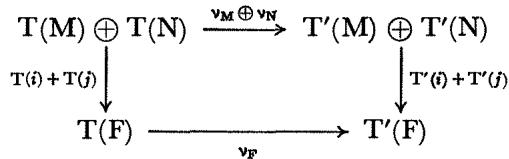
\includegraphics[keepaspectratio]{images/part002_2544dc0c.jpg}}

is commutative and the vertical arrows are bijective.

The commutativity follows from Lemma 1, the other assertions from § 1, no. 6, Corollary 2 to Proposition 6 and § 3, no. 7, Proposition 7.

Lemma 3. Under the hypotheses of Lemma 2, for \(\nu_{\mathrm{F}}\) to be injective (resp. surjective), it is necessary and sufficient that \(\nu_{\mathrm{M}}\) and \(\nu_{\mathrm{N}}\) be so.

This follows from Lemma 2 and § 1, no. 6, Corollary 1 to Proposition 6.

Then Lemma 3, together with §2, no. 2, Proposition 4, shows that it suffices to consider the case where F is a free module. But, if \((b_{\mu})\) is a basis of F, every element of \(\operatorname{Hom}_{\mathbf{A}}(\mathbf{E}, \mathbf{G}) \otimes_{\mathbf{B}} \mathbf{F}\) may then be written uniquely as \(\sum_{\mu} u_{\mu} \otimes b_{\mu}\) , where \(u_{\mu} \in \operatorname{Hom}_{\mathbf{A}}(\mathbf{E}, \mathbf{G})\) (§ 3, no. 7, Corollary 1 to Proposition 7); the image of this element under \(\nu\) is the A-linear mapping \(x \mapsto \sum_{\mu} u_{\mu}(x) \otimes b_{\mu}\) ; it cannot be zero for all \(x \in \mathbf{E}\) unless \(u_{\mu}(x) = 0\) for all \(x \in \mathbf{E}\) and all \(\mu\) , which is equivalent to saying that \(u_{\mu} = 0\) for all \(\mu\) ; hence \(\nu\) is injective. When also F admits a finite basis, Lemma 3 shows (by induction on the number of elements in the basis of F) that to prove that \(\nu\) is surjective, it suffices to do so when \(F = B_s\) ; but in this case the two sides of (7) are canonically identified with \(\operatorname{Hom}_{\mathbf{A}}(\mathbf{E}, \mathbf{G})\) (§ 3, no. 4, Proposition 4) and \(\nu\) becomes the identity.

\begin{enumerate}
\def\labelenumi{(\roman{enumi})}
\setcounter{enumi}{1}
\tightlist
\item
  To show the proposition when E is projective and finitely generated, this time we fix F and G and write, for every left A-module E,
\end{enumerate}

\[
\mathrm{T} (\mathrm{E}) = \operatorname{Hom} _ {\mathrm{A}} (\mathrm{E}, \mathrm{G}) \otimes_ {\mathrm{B}} \mathrm{F}, \quad \mathrm{T} ^ {\prime} (\mathrm{E}) = \operatorname{Hom} _ {\mathrm{A}} (\mathrm{E}, \mathrm{G} \otimes_ {\mathrm{B}} \mathrm{F})
\]

and, for every left A-module homomorphism \(v:\mathbf{E}\to\mathbf{E}^{\prime}\) ,

\[
\mathrm{T} (v) = \operatorname{Hom} (v, 1 _ {\mathbf {G}}) \otimes 1 _ {\mathbf {F}}, \quad \mathrm{T} ^ {\prime} (v) = \operatorname{Hom} (v, 1 _ {\mathbf {G}} \otimes 1 _ {\mathbf {F}});
\]

on the other hand, we write \(\nu_{E}\) instead of \(\nu\). Then we have the two lemmas:

Lemma 4. For every homomorphism \(v: \mathbf{E} \to \mathbf{E}'\) , the diagram

\[
\begin{array}{c c c} \mathrm{T} (\mathrm{E} ^ {\prime}) & \xrightarrow {\nu_ {\mathrm{E} ^ {\prime}}} & \mathrm{T} ^ {\prime} (\mathrm{E} ^ {\prime}) \\ \mathrm{T} (v) \Big \downarrow & & \Big \downarrow \mathrm{T} ^ {\prime} (v) \\ \mathrm{T} (\mathrm{E}) & \xrightarrow {\nu_ {\mathrm{E}}} & \mathrm{T} ^ {\prime} (\mathrm{E}) \end{array}\tag{10}
\]

is commutative.

Lemma 5. Let \(\mathbf{M}\) and \(\mathbf{N}\) be two supplementary submodules in \(\mathbf{E}\) and \(p: \mathbf{E} \to \mathbf{M}\) , \(q: \mathbf{E} \to \mathbf{N}\) the canonical projections. The diagram

\pandocbounded{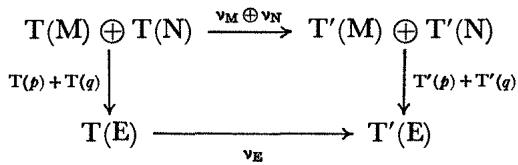
\includegraphics[keepaspectratio]{images/part002_a961576f.jpg}}

is commutative and the vertical arrows are bijective.

They are proved as Lemmas 1 and 2, taking account of § 1, no. 6, Corollary 2 to Proposition 6, § 2, no. 1, Proposition 1 and § 3, no. 7, Proposition 7.

The remainder of the proof then proceeds as in (i) and is reduced to the case where \(E = A_{s}\) ; the two sides of (7) are then canonically identified with \(G \otimes_{B} F\) and \(\nu\) becomes the identity.

In particular take B = A and G the (A, A)-bimodule \(_{s}A_{d}\) (§ 3, no. 4), so that the right A-module \(\operatorname{Hom}_{\mathbf{A}}(\mathbf{E}, _{s}\mathbf{A}_{d})\) is just the dual E* of E and \((_{s}\mathbf{A}_{d}) \otimes_{\mathbf{A}} F\) is canonically identified with F (§ 3, no. 4, Proposition 4). Homomorphism (7) then becomes a canonical Z-homomorphism

\[
\theta : \mathrm{E} ^ {*} \otimes_ {\mathrm{A}} \mathrm{F} \rightarrow \operatorname{Hom} _ {\mathrm{A}} (\mathrm{E}, \mathrm{F})\tag{11}
\]

and \(\theta (x^{*}\otimes y)\) is the linear mapping of E into F

\[
x \mapsto \langle x, x ^ {*} \rangle y.
\]

Remark (1). The characterization of projective A-modules given in §2, no. 6, Proposition 12, can also be expressed as follows: for a left A-module E to be projective, it is necessary and sufficient that the canonical homomorphism

\[
\theta_ {\mathbf {E}}: \mathrm{E} ^ {*} \otimes_ {\mathbf {A}} \mathrm{E} \rightarrow \operatorname{Hom} _ {\mathbf {A}} (\mathrm{E}, \mathrm{E}) = \operatorname{End} _ {\mathbf {A}} (\mathrm{E})
\]

be such that \(l_{E}\) belongs to the image of \(\theta_{E}\) .

COROLLARY. (i) When F is a projective (resp. finitely generated projective) module, the canonical homomorphism (11) is injective (resp. bijective).

\begin{enumerate}
\def\labelenumi{(\roman{enumi})}
\setcounter{enumi}{1}
\tightlist
\item
  When E is a finitely generated projective module, the canonical homomorphism (11) is bijective.
\end{enumerate}

Even when E and F are both finitely generated, \(\theta\) is not necessarily surjective, as is shown by the example A = Z, E = F = Z/2Z; the right hand side of (11) is non-zero but \(E^{*} = 0\) . On the other hand, examples can be given where E is free, but (11) is neither injective nor surjective (Exercise 3(b)).

When E admits a finite basis \((e_i)\) , the inverse isomorphism \(\theta^{-1}\) of \(\theta\) can be found explicitly as follows. Let \((e_i^*)\) be the dual basis of \((e_i)\) (§ 2, no. 6); for all \(u \in \operatorname{Hom}(\mathbf{E}, \mathbf{F})\) and all \(x = \sum_{i} \xi_i e_i\) with \(\xi_i \in \mathbf{A}\) ,

\[
u (x) = \sum_ {i} \xi_ {i} u (e _ {i}) = \sum_ {i} \langle x, e _ {i} ^ {*} \rangle u (e _ {i})
\]

and therefore \(u = \sum_{i} \theta(e_i^* \otimes u(e_i))\) , in other words

\[
\theta^ {- 1} (u) = \sum_ {i} e _ {i} ^ {*} \otimes u (e _ {i}).\tag{12}
\]

In particular, if further F = E, it is seen that the image under \(\theta_{E}^{-1}\) of the identity mapping \(l_{E}\) is the element \(\sum_{i} e_{i}^{*} \otimes e_{i}\) , which is therefore independent of the basis \((e_{i})\) considered in E.

Note on the other hand that when E is a finitely generated projective module the ring structure on \(\operatorname{End}_{\mathbf{A}}(\mathbf{E})\) can be transported by \(\theta_{E}^{-1}\) to \(E^{*}\otimes_{A}E\) ; it is immediately verified that, for x, y in E, \(x^{*}, y^{*}\) in \(E^{*}\) , in the ring \(\operatorname{End}_{\mathbf{A}}(\mathbf{E})\) ,

\[
\theta_ {\mathbf {E}} (x ^ {*} \otimes x) \circ \theta_ {\mathbf {E}} (y ^ {*} \otimes y) = \theta_ {\mathbf {E}} ((y ^ {*} \langle y, x ^ {*} \rangle) \otimes x).\tag{13}
\]

Remark (2). Let E be a right A-module; replacing E by E* in (11), we obtain a canonical Z-homomorphism

\[
\mathrm{E} ^ {* *} \otimes_ {\mathrm{A}} \mathrm{F} \rightarrow \operatorname{Hom} _ {\mathrm{A}} (\mathrm{E} ^ {*}, \mathrm{F}).\tag{14}
\]

On the other hand, there is a canonical A-homomorphism \(c_{E}:E\to E^{**}\) , whence there is a Z-homomorphism \(c_{E}\otimes l_{F}:E\otimes_{A}F\to E^{**}\otimes_{A}F\) ; composing the latter with the homomorphism (14), we hence obtain a canonical Z-homomorphism

\[
\theta^ {\prime}: \mathrm{E} \otimes_ {\mathrm{A}} \mathrm{F} \rightarrow \operatorname{Hom} _ {\mathrm{A}} (\mathrm{E} ^ {*}, \mathrm{F})\tag{15}
\]

such that \(\theta'(x \otimes y)\) is the linear mapping

\[
x ^ {*} \mapsto \langle x, x ^ {*} \rangle y.
\]

If E and F are projective modules, the mapping (15) is injective. For \(c_{E}\) is then injective (§2, no. 7, Corollary 4 to Proposition 13) and as F is projective, the Z-homomorphism \(c_{E} \otimes l_{F}: E \otimes_{A} F \to E^{**} \otimes_{A} F\) is also injective (§3, no. 7, Corollary 6 to Proposition 7); finally, it has been seen (Proposition 2) that the homomorphism (14) is injective, whence the conclusion.

If E is projective and finitely generated, the mapping (15) is bijective for the two mappings of which it is composed are then bijective (§ 2, no. 7, Corollary 4 to Proposition 13 and Proposition 2 above).

\subsection{TRACE OF AN ENDOMORPHISM}

Let C be a commutative ring and E a C-module. The mapping \((x^{*}, x) \mapsto \langle x, x^{*} \rangle\) of \(E^{*} \times E\) into C is then C-bilinear, since, for all \(\gamma \in C\) , \(\langle \gamma x, x^{*} \rangle = \gamma \langle x, x^{*} \rangle\) and \(\langle x, x^{*} \gamma \rangle = \langle x, x^{*} \rangle \gamma\) ; we derive a canonical C-linear mapping

\[
\tau : \mathbf {E} ^ {*} \otimes_ {\mathbf {c}} \mathbf {E} \rightarrow \mathbf {C}\tag{16}
\]

such that \(\tau(x^{*} \otimes x) = \langle x, x^{*} \rangle\) (§ 3, no. 5). Suppose now also that E is a finitely generated projective C-module; the canonical isomorphism (11) of no. 2 is then a C-module isomorphism and we can therefore define by transporting the structure a canonical linear form \(\mathrm{Tr} = \tau \circ \theta_{\mathbf{E}}^{-1}\) on the C-module \(\operatorname{End}_{\mathbf{C}}(\mathbf{E})\) . For all \(u \in \operatorname{End}_{\mathbf{C}}(\mathbf{E})\) the scalar \(\operatorname{Tr}(u)\) is called the trace of the endomorphism \(u\) ; every \(u \in \operatorname{End}_{\mathbf{C}}(\mathbf{E})\) can be written (in general in an infinity of ways) in the form \(x \mapsto \sum_{i} \langle x, x_{i}^{*} \rangle y_{i}\) where \(x_{i}^{*} \in \mathbf{E}^{*}\) and \(y_{i} \in \mathbf{E}_{i}\) by virtue of no. 2, Corollary to Proposition 2; then

\[
\operatorname{Tr} (u) = \sum_ {i} \left\langle y _ {i}, x _ {i} ^ {*} \right\rangle \quad (\text { cf. } \S 1 0, \text { no. } 1 1).\tag{17}
\]

By definition,

\begin{enumerate}
\def\labelenumi{(\arabic{enumi})}
\setcounter{enumi}{17}
\tightlist
\item
\end{enumerate}

\[
\operatorname{Tr} (u + v) = \operatorname{Tr} (u) + \operatorname{Tr} (v)\tag{19}
\]

\[
\operatorname{Tr} (\gamma u) = \gamma \operatorname{Tr} (u)
\]

for \(u, v\) in \(\operatorname{End}_{\mathbf{C}}(\mathbf{E})\) and \(\gamma \in \mathbf{C}\) . Moreover:

PROPOSITION 3. Let C be a commutative ring, E, F two finitely generated projective C-modules and \(u: \mathbf{E} \to \mathbf{F}\) and \(v: \mathbf{F} \to \mathbf{E}\) two linear mappings; then

\[
\operatorname{Tr} (v \circ u) = \operatorname{Tr} (u \circ v).\tag{20}
\]

The two mappings \((u, v) \mapsto \operatorname{Tr}(u \circ v)\) , \((u, v) \mapsto \operatorname{Tr}(v \circ u)\) of

\[
\operatorname{Hom} _ {\mathbf {c}} (\mathbf {E}, \mathbf {F}) \times \operatorname{Hom} _ {\mathbf {c}} (\mathbf {F}, \mathbf {E})
\]

into C are C-bilinear; it therefore suffices to verify (20) when u is of the form \(x \mapsto \langle x, a^{*} \rangle b\) and v of the form \(y \mapsto \langle y, b^{*} \rangle a\) , with \(a \in E\) , \(a^{*} \in E^{*}\) , \(b \in F\) , \(b^{*} \in F^{*}\) . But then \(v \circ u\) is the mapping \(x \mapsto \langle x, a^{*} \rangle \langle b, b^{*} \rangle a\) and \(u \circ v\) the mapping \(y \mapsto \langle y, b^{*} \rangle \langle a, a^{*} \rangle b\) . Formula (17) shows that the values of the two sides of (20) are equal to \(\langle a, a^{*} \rangle \langle b, b^{*} \rangle\) .

COROLLARY. If \(u_1, \ldots, u_p\) are endomorphisms of \(\mathbf{E}\) , then

\[
\operatorname{Tr} \left(u _ {1} \circ u _ {2} \circ \dots \circ u _ {p}\right) = \operatorname{Tr} \left(u _ {i} \circ u _ {i + 1} \circ \dots \circ u _ {p} \circ u _ {1} \circ \dots \circ u _ {i - 1}\right)
\]

for \(1 \leqslant i \leqslant p\) (``invariance of the trace under cyclic permutation'').

It suffices to apply (20) to the product

\[
\left(u _ {1} \circ u _ {2} \circ \dots \circ u _ {i - 1}\right) \circ \left(u _ {i} \circ u _ {i + 1} \circ \dots \circ u _ {p}\right).
\]

Note that on the other hand it is not necessarily true that

\[
\operatorname{Tr} (u \circ v \circ w) = \operatorname{Tr} (u \circ w \circ v)
\]

for three endomorphisms u, v, w of E.

\subsection{\texorpdfstring{THE HOMOMORPHISM \(\operatorname{Hom}_{\mathbb{C}}(\mathrm{E}_1, \mathrm{F}_1) \otimes_{\mathbb{C}} \operatorname{Hom}_{\mathbb{C}}(\mathrm{E}_2, \mathrm{F}_2) \to \operatorname{Hom}_{\mathbb{C}}(\mathrm{E}_1 \otimes_{\mathbb{C}} \mathrm{E}_2, \mathrm{F}_1 \otimes_{\mathbb{C}} \mathrm{F}_2)\)}{The homomorphism from Hom over C of E1,F1 tensor Hom over C of E2,F2 to Hom over C of the corresponding tensor products}}

Let C be a commutative ring and \(E_{1}\) , \(E_{2}\) , \(F_{1}\) , \(F_{2}\) four C-modules; in §3, no. 5, formula (13) we defined a canonical C-module homomorphism

\[
\lambda : \operatorname{Hom} (\mathbf {E} _ {1}, \mathbf {F} _ {1}) \otimes \operatorname{Hom} (\mathbf {E} _ {2}, \mathbf {F} _ {2}) \to \operatorname{Hom} (\mathbf {E} _ {1} \otimes \mathbf {E} _ {2}, \mathbf {F} _ {1} \otimes \mathbf {F} _ {2}). \tag {21}
\]

PROPOSITION 4. When one of the ordered pairs \((\mathbf{E}_1, \mathbf{E}_2)\) , \((\mathbf{E}_1, \mathbf{F}_1)\) , \((\mathbf{E}_2, \mathbf{F}_2)\) consists of finitely generated projective C-modules, the canonical homomorphism (21) is bijective.

It is obviously sufficient to perform the proof for the ordered pairs \((\mathbf{E}_{1}, \mathbf{F}_{1})\) and \((\mathbf{E}_{1}, \mathbf{E}_{2})\) .

We consider first the case of the ordered pair \((\mathbf{E}_1, \mathbf{F}_1)\) ; we fix \(\mathbf{E}_2, \mathbf{F}_1, \mathbf{F}_2\) and write for every C-module \(\mathrm{T}(\mathbf{E}) = \mathrm{Hom}(\mathbf{E}, \mathbf{F}_1) \otimes_{\mathbb{C}} \mathrm{Hom}(\mathbf{E}_2, \mathbf{F}_2)\) and \(\mathrm{T}'(\mathbf{E}) = \mathrm{Hom}(\mathbf{E} \otimes \mathbf{E}_2, \mathbf{F}_1 \otimes \mathbf{F}_2)\) and, for every C-homomorphism \(v: \mathbf{E} \to \mathbf{E}'\) ,

\[
\mathrm{T} (v) = \operatorname{Hom} (v, \mathrm{l} _ {\mathrm{F} _ {1}}) \otimes \mathrm{l} _ {\operatorname{Hom} (\mathrm{E} _ {2}, \mathrm{F} _ {2})}
\]

and

\[
\mathrm{T} ^ {\prime} (v) = \operatorname{Hom} (v \otimes 1 _ {\mathbb {E} _ {2}}, 1 _ {\mathbf {F} _ {1} \otimes \mathbf {F} _ {2}}).
\]

Then Lemmas 4 and 5 (no. 2) (where v is replaced by λ) are valid and are proved by completely analogous methods.

We next fix \(\mathbf{E}_2\) and \(\mathbf{F}_2\) and this time write, for every C-module \(\mathbf{F}\) , \(\mathrm{T}(\mathbf{F}) = \mathrm{Hom}(\mathbf{C},\mathbf{F})\otimes_{\mathbb{C}}\mathrm{Hom}(\mathbf{E}_2,\mathbf{F}_2)\) and \(\mathrm{T}'(\mathrm{F}) = \mathrm{Hom}(\mathbf{C}\otimes \mathbf{E}_2,\mathbf{F}\otimes \mathbf{F}_2)\) and, for every C-homomorphism \(u:\mathrm{F}\to \mathrm{F}'\) ,

\[
\mathrm{T} (u) = \operatorname{Hom} (\mathrm{l} _ {\mathbf {c}}, u) \otimes \mathrm{l} _ {\operatorname{Hom} (\mathbb {E} _ {2}, \mathrm{F} _ {2})}
\]

and

\[
\mathrm{T} ^ {\prime} (u) = \operatorname{Hom} (\mathrm{l} _ {\mathrm{c}} \otimes \mathrm{l} _ {\mathrm{E} _ {2}}, u \otimes \mathrm{l} _ {\mathrm{F} _ {2}}).
\]

This time it is immediately verified that Lemmas 1 and 2 (no. 2) (where \(\lambda\) always replaces \(\nu\) ) are valid.

This being so, we show the proposition first when \(E_{1} = C\) and \(F_{1}\) is projective and finitely generated. The argument of no. 2 (which rests on Lemmas 1 and 2), together with the above remarks, reduces this to proving the proposition when also \(F_{1} = C\) ; then \(\operatorname{Hom}(E_{1}, F_{1})\) , \(E_{1} \otimes E_{2}\) and \(F_{1} \otimes F_{2}\) are identified with C, \(E_{2}\) and \(F_{2}\) respectively (§ 3, no. 4, Proposition 4); the two sides of (21) are then both canonically identified with \(\operatorname{Hom}(\mathbf{E}_{2},\mathbf{F}_{2})\) and, after these identifications, it is verified that \(\lambda\) becomes the identity.

We now suppose that \(F_{1}\) is projective and finitely generated; the argument of no. 2 (depending this time on Lemmas 4 and 5) reduces the proof for \(E_{1}\) any finitely generated projective module to the case where \(E_{1} = C\) , that is to the first case dealt with.

For the ordered pair \((\mathbf{E}_{1}, \mathbf{E}_{2})\) , the procedure is similar, this time applying Lemmas 4 and 5 twice; we leave the details to the reader.

Note that when \(\mathbf{E}_1 = \mathbf{C}^{(I)}\) , \(\mathbf{E}_2 = \mathbf{C}^{(J)}\) are free (finitely generated or not), then \(\operatorname{Hom}(\mathbf{E}_1, \mathbf{F}_1) = \mathbf{F}_1^{\mathrm{I}}\) , \(\operatorname{Hom}(\mathbf{E}_2, \mathbf{F}_2 = \mathbf{F}_2^{\mathrm{J}}\) and

\[
\operatorname{Hom} \left(\mathrm{E} _ {1} \otimes \mathrm{E} _ {2}, \mathrm{F} _ {1} \otimes \mathrm{F} _ {2}\right) = \left(\mathrm{F} _ {1} \otimes \mathrm{F} _ {2}\right) ^ {\mathrm{I} \times \mathrm{J}}
\]

to within canonical isomorphisms and (21) is then identical with a special case of the canonical homomorphism (22) of § 3, no. 7.

When \(E_{2} = C\) , the canonical homomorphism (21) gives, after identifying \(\operatorname{Hom}(E_{2}, F_{2})\) with \(F_{2}\) and \(E_{1} \otimes E_{2}\) with \(E_{1}\) , a canonical homomorphism

\[
\operatorname{Hom} (\mathrm{E}, \mathrm{F}) \otimes \mathrm{G} \rightarrow \operatorname{Hom} (\mathrm{E}, \mathrm{F} \otimes \mathrm{G})\tag{22}
\]

for any three C-modules E, F, G which is just the homomorphism (7) of no. 2 for \(\mathbf{A} = \mathbf{B} = \mathbf{C}\) .

Note that when \(\mathbf{F} = \mathbf{C}\) the canonical homomorphism (22) again gives (11) (no. 2) for the case of a commutative ring.

Suppose now that \(\mathbf{F}_1 = \mathbf{F}_2 = \mathbf{C}\) ; as \(\mathbf{F}_1 \otimes \mathbf{F}_2\) is identified with \(\mathbf{C}\) , there is this time a canonical homomorphism

\[
\mu : \mathbf {E} ^ {*} \otimes \mathbf {F} ^ {*} \rightarrow (\mathbf {E} \otimes \mathbf {F}) ^ {*}\tag{23}
\]

for two C-modules E, F; for \(x^{*} \in \mathbf{E}^{*}\) , \(y^{*} \in \mathbf{F}^{*}\) , the image of \(x^{*} \otimes y^{*}\) under the canonical homomorphism (23) is the linear form \(u\) on \(\mathbf{E} \otimes \mathbf{F}\) such that

\[
u (x \otimes y) = \langle x, x ^ {*} \rangle \langle y, y ^ {*} \rangle .\tag{24}
\]

Moreover, if \(E_{1}\) , \(E_{2}\) , \(F_{1}\) , \(F_{2}\) are four C-modules, \(f: E_{1} \rightarrow E_{2}\) , \(g: F_{1} \rightarrow F_{2}\) two linear mappings, it follows immediately from (24) that the diagram

\[
\begin{array}{c} \mathrm{E} _ {2} ^ {*} \otimes \mathrm{F} _ {2} ^ {*} \xrightarrow {\mu} (\mathrm{E} _ {2} \otimes \mathrm{F} _ {2}) ^ {*} \\ t _ {f} \otimes t _ {g} \Biggl \downarrow \qquad \qquad \qquad \qquad \qquad \qquad \qquad \qquad \qquad \qquad \qquad \qquad \qquad \qquad \qquad \qquad \qquad \qquad \qquad \qquad \qquad \qquad \qquad \qquad \qquad \qquad \qquad \qquad \qquad \qquad \qquad \qquad \qquad \qquad \\ \mathrm{E} _ {1} ^ {*} \otimes \mathrm{F} _ {1} ^ {*} \xrightarrow {\mu} (\mathrm{E} _ {1} \otimes \mathrm{F} _ {1}) ^ {*} \end{array}\tag{25}
\]

is commutative.

COROLLARY 1. If one of the modules E, F is projective and finitely generated, the canonical homomorphism (23) is bijective.

COROLLARY 2. Let \(\mathbf{E}_1, \mathbf{E}_2\) be two finitely generated projective C-modules, \(u_1\) an endomorphism of \(\mathbf{E}_1\) and \(u_2\) an endomorphism of \(\mathbf{E}_2\) ; then

\[
\operatorname{Tr} (u _ {1} \otimes u _ {2}) = \operatorname{Tr} (u _ {1}) \operatorname{Tr} (u _ {2}).\tag{26}
\]

By linearity, it suffices to consider the case where \(u_{1}\) is of the form \(x_{1} \mapsto \langle x_{1}, x_{1}^{*} \rangle y_{1}\) and \(u_{2}\) of the form \(x_{2} \mapsto \langle x_{2}, x_{2}^{*} \rangle y_{2}\) ; then the image of \(x_{1} \otimes x_{2}\) under \(u_{1} \otimes u_{2}\) is by definition

\[
\langle x _ {1}, x _ {1} ^ {*} \rangle \langle x _ {2}, x _ {2} ^ {*} \rangle (y _ {1} \otimes y _ {2}) = \langle x _ {1} \otimes x _ {2}, x _ {1} ^ {*} \otimes x _ {2} ^ {*} \rangle (y _ {1} \otimes y _ {2})
\]

\(x_{1}^{*}\otimes x_{2}^{*}\) being canonically identified under \(\mu\) with an element of \((\mathrm{E}_{1}\otimes\mathrm{E}_{2})^{*}\) . As \(\langle y_{1}\otimes y_{2},x_{1}^{*}\otimes x_{2}^{*}\rangle=\langle y_{1},x_{1}^{*}\rangle\langle y_{2},x_{2}^{*}\rangle\) , formula (26) follows in this case from (17).

Remark. If E, F, G are any three C-modules, it is immediately verified that the diagram

\[
\begin{array}{c} \mathrm{E} ^ {*} \otimes \mathrm{F} ^ {*} \otimes \mathrm{G} ^ {*} \xrightarrow {\mu \otimes 1} (\mathrm{E} \otimes \mathrm{F}) ^ {*} \otimes \mathrm{G} ^ {*} \\ 1 \otimes \mu \Biggl \downarrow \\ \mathrm{E} ^ {*} \otimes (\mathrm{F} \otimes \mathrm{G}) ^ {*} \xrightarrow [ \mu ]{} (\mathrm{E} \otimes \mathrm{F} \otimes \mathrm{G}) ^ {*} \end{array}\tag{27}
\]

is commutative, by virtue of formula (24).

We note also that, without any hypothesis on the C-modules E, F, there are canonical isomorphisms

\begin{enumerate}
\def\labelenumi{(\arabic{enumi})}
\setcounter{enumi}{27}
\tightlist
\item
\end{enumerate}

\[
(\mathbf {E} \otimes \mathbf {F}) ^ {*} \rightarrow \operatorname{Hom} (\mathbf {E}, \mathbf {F} ^ {*})\tag{29}
\]

\[
(\mathbf {E} \otimes \mathbf {F}) ^ {*} \rightarrow \operatorname{Hom} (\mathbf {F}, \mathbf {E} ^ {*})
\]

which are just the isomorphism (6) and (5) of no. 1 for \(\mathbf{G} = \mathbf{C}\) , \(\mathbf{A} = \mathbf{B} = \mathbf{C}\) .

Thus a canonical one-to-one correspondence has been defined between the bilinear forms on \(E \times F\) , the homomorphisms of E into \(F^{*}\) and the homomorphisms of F into \(E^{*}\) : if u (resp. v) is a homomorphism of E into \(F^{*}\) (resp. of F into \(E^{*}\) ), the corresponding bilinear form is given by

\[
(x, y) \mapsto \langle y, u (x) \rangle \quad (\text { resp. } (x, y) \mapsto \langle x, v (y) \rangle).
\]

\section{EXTENSION OF THE RING OF SCALARS}

\subsection{EXTENSION OF THE RING OF SCALARS OF A MODULE}

Let A, B be two rings and \(\rho: \mathbf{A} \to \mathbf{B}\) a ring homomorphism; we consider the right A-module \(\rho^{*}(B_{d})\) defined by this homomorphism (§ 1, no. 13); this A-module also has a left B-module structure, namely that of \(B_{s}\) and, as \(b'(b\rho(a)) = (b'b)\rho(a)\) for \(a \in \mathbf{A}\) , \(b\) , \(b'\) in B, these two module structures on B are compatible (§ 1, no. 14). This allows us, for every left A-module E, to define a left B-module structure on the tensor product \(\rho_{*}(B_{d}) \otimes_{\mathbf{A}} \mathbf{E}\) such that \(\beta'(\beta \otimes x) = (\beta'\beta) \otimes x\) for \(\beta\) , \(\beta'\) in B and \(x \in \mathbf{E}\) (§ 3, no. 3). This left B-module is said to be derived from E by extending the ring of scalars to B by means of \(\rho\) and it is denoted by \(\rho^{*}(\mathbf{E})\) or \(\mathrm{E}_{(\mathbf{B})}\) if no confusion arises.

PROPOSITION 1. For every left A-module E, the mapping \(\phi: x \mapsto 1 \otimes x\) of E into the A-module \(\rho_*(\rho^*(\mathbf{E}))\) is A-linear and the set \(\phi(\mathbf{E})\) generates the B-module \(\rho^*(\mathbf{E})\) . Further, for every left B-module F and every A-linear mapping \(f\) of E into the A-module \(\rho_*(\mathbf{F})\) , there exists one and only one B-linear mapping \(\tilde{f}\) of \(\rho^*(\mathbf{E})\) into F such that \(\tilde{f}(1 \otimes x) = f(x)\) for all \(x \in \mathbf{E}\) .

B can be considered as a (B, A)-bimodule by means of \(\rho\) ; then there is a canonical Z-module isomorphism

\[
\operatorname{Hom} _ {\mathbf {B}} (\mathbf {B} \otimes_ {\mathbf {A}} \mathbf {E}, \mathbf {F}) \rightarrow \operatorname{Hom} _ {\mathbf {A}} (\mathbf {E}, \operatorname{Hom} _ {\mathbf {B}} (\mathbf {B} _ {s}, \mathbf {F}))\tag{1}
\]

as has been seen in § 4, no. 1, Proposition 1. But the left A-module \(\mathrm{Hom}_{\mathbf{B}}(\mathbf{B}_{s},\mathbf{F})\) is canonically identified with \(\rho^{*}(\mathbf{F})\) : for, by definition (§ 1, no. 14), there corresponds to an element \(y\in \mathbf{F}\) the homomorphism \(\theta (y)\colon \mathbf{B}_s\to \mathbf{F}\) such that \((\theta (y))(1) = y\) ; for all \(\lambda \in \mathbf{A}\) , there thus corresponds to \(\rho (\lambda)y\in \mathbf{F}\) the homomorphism \(\mu \mapsto \mu \rho (\lambda)y\) of \(\mathbf{B}_s\) into \(\mathbf{F}\) , which is just \(\lambda \theta (y)\) for the left A-module structure on \(\mathrm{Hom}_{\mathbf{B}}(\mathbf{B}_{s},\mathbf{F})\) (§ 1, no. 14). Using this identification, we obtain therefore a canonical Z-module isomorphism, the inverse of (1)

\[
\delta : \operatorname{Hom} _ {\mathbf {A}} (\mathbf {E}, \rho_ {*} (\mathbf {F})) \rightarrow \operatorname{Hom} _ {\mathbf {B}} (\rho^ {*} (\mathbf {E}), \mathbf {F})\tag{2}
\]

and it follows immediately from the definitions that if \(\delta(f) = \bar{f}\) then \(\bar{f}(1 \otimes x) = f(x)\) for all \(x \in \mathbf{E}\) . In particular, the mapping \(\phi_{\mathbb{E}}: x \mapsto 1 \otimes x\) is just

\[
\phi_ {\mathbf {E}} = \delta^ {- 1} (1 _ {\rho^ {*} (\mathbf {E})}).\tag{3}
\]

Proposition 1 is therefore proved. The mapping \(\phi_{\mathbf{E}}: \mathbf{E} \to \rho_{*}(\rho^{*}(\mathbf{E}))\) is called canonical.

Remarks. (1) Proposition 1 shows that the ordered pair consisting of \(\mathbf{E}_{(\mathbf{B})}\) and \(\phi_{\mathbb{E}}\) is a solution of the universal mapping problem (Set Theory, IV, §3, no. 1), where \(\Sigma\) is the species of left B-module structures (the morphisms being B-linear mappings) and the \(\alpha\) -mappings are the A-linear mappings of E into a B-module.

\begin{enumerate}
\def\labelenumi{(\arabic{enumi})}
\setcounter{enumi}{1}
\item
  If E is an \((\mathbf{A}, (\mathbf{C}_{i}^{\prime}); (\mathbf{D}_{j}^{\prime}))\) -multimodule and F a \((\mathbf{B}, (\mathbf{C}_{h}^{\prime\prime}); (\mathbf{D}_{k}^{\prime\prime}))\) -multimodule, then the isomorphism (2) is linear with respect to the \(((\mathbf{D}_{j}^{\prime}), (\mathbf{C}_{h}^{\prime\prime}); (\mathbf{C}_{i}^{\prime}), (\mathbf{D}_{k}^{\prime\prime}))\) -multimodule structures of the two sides (§ 1, no. 14 and § 3, no. 4).
\item
  Let E be a left A-module, a a two-sided ideal of A and \(\rho:A\to A/a\) the canonical homomorphism. In the notation of §3, no. 6, Corollary 2 to Proposition 6, the A-module E/aE is annihilated by a and therefore has canonically a left (A/a)-module structure (§1, no. 12); it is immediate that the canonical mapping \(\pi:\rho^{*}(E)\to E/aE\) defined in §3, no. 6, Corollary 2 to Proposition 6 is an isomorphism for the (A/a)-module structures.
\end{enumerate}

COROLLARY. Let E, E' be two left A-modules; for every A-linear mapping u: E → E', v = l\_B ⊗ u is the unique B-linear mapping which renders commutative the diagram

\pandocbounded{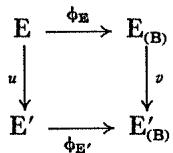
\includegraphics[keepaspectratio]{images/part002_74d11806.jpg}}

where \(\phi_{\mathbf{E}}\) and \(\phi_{\mathbf{E}'}\) are the canonical mappings.

It suffices to apply Proposition 1 to the A-homomorphism \(\phi_{\mathbf{E}'} \circ u: \mathbf{E} \to \mathbf{E}_{(\mathbf{B})}'\) .

The mapping \(v\) defined in the above corollary is denoted by \(\rho^{*}(u)\) or \(u_{(B)}\) . If \(E''\) is a third left A-module and \(v: E' \to E''\) an A-linear mapping, it is immediate that

\[
\left(v \circ u\right) _ {(\mathbf {B})} = v _ {(\mathbf {B})} \circ u _ {(\mathbf {B})}.
\]

Extending the ring of operators of a module is a transitive operation; to be precise:

PROPOSITION 2. Let \(\rho: \mathbf{A} \to \mathbf{B}\) , \(\sigma: \mathbf{B} \to \mathbf{C}\) be ring homomorphisms. For every left A-module E, there exists one and only one C-homomorphism

\[
\sigma^ {*} (\rho^ {*} (\mathrm{E})) \rightarrow (\sigma \circ \rho) ^ {*} (\mathrm{E})\tag{4}
\]

mapping \(1 \otimes (1 \otimes x)\) to \(1 \otimes x\) for all \(x \in E\) and this homomorphism is bijective.

The underlying Z-modules of \(\sigma^{*}(\rho^{*}(\mathbf{E}))\) and \((\sigma \circ \rho)^{*}(\mathbf{E})\) are respectively \(\mathbf{C} \otimes_{\mathbf{B}} (\mathbf{B} \otimes_{\mathbf{A}} \mathbf{E})\) and \(\mathbf{C} \otimes_{\mathbf{A}} \mathbf{E}\) . There exists a canonical Z-isomorphism \(\mathbf{C} \otimes_{\mathbf{B}} (\mathbf{B} \otimes_{\mathbf{A}} \mathbf{E}) \to (\mathbf{C} \otimes_{\mathbf{B}} \mathbf{B}) \otimes_{\mathbf{A}} \mathbf{E}\) (§ 3, no. 8, Proposition 8), which is also a C-isomorphism for the left C-module structures on both sides. Moreover, the C-module C ⊗B B is canonically identified with the C-module Cs under the isomorphism which maps γ ⊗ β to γσ(β) (§ 3, no. 4, Proposition 4) and this isomorphism is also an isomorphism for the right A-module structure on C ⊗B B defined by ρ and the right A-module structure on C defined by σ ∘ ρ. Thus a canonical isomorphism

\[
(\mathbf {C} \otimes_ {\mathbf {B}} \mathbf {B}) \otimes_ {\mathbf {A}} \mathbf {E} \rightarrow \mathbf {C} \otimes_ {\mathbf {A}} \mathbf {E}
\]

is obtained and, composing it with the isomorphism

\[
\mathbf {C} \otimes_ {\mathbf {B}} (\mathbf {B} \otimes_ {\mathbf {A}} \mathbf {E}) \rightarrow (\mathbf {C} \otimes_ {\mathbf {B}} \mathbf {B}) \otimes_ {\mathbf {A}} \mathbf {E}
\]

defined earlier, the desired canonical isomorphism is obtained.

If \(\phi, \phi'\) and \(\phi''\) denote the canonical mappings \(E \to \rho^*(E)\) , \(\rho^*(E \to) \sigma^*(\rho^*(E))\) and \(E \to (\sigma \circ \rho)^*(E)\) , \(\phi' \circ \phi\) is identified with \(\phi''\) under the canonical isomorphism of Proposition 2.

PROPOSITION 3. Let A, B be two commutative rings, \(\rho: \mathbf{A} \to \mathbf{B}\) a ring homomorphism and E, E' two A-modules. There exists one and only one B-homomorphism

\[
\mathbf {E} _ {(\mathbf {B})} \otimes_ {\mathbf {B}} \mathbf {E} _ {(\mathbf {B})} ^ {\prime} \rightarrow (\mathbf {E} \otimes_ {\mathbf {A}} \mathbf {E} ^ {\prime}) _ {(\mathbf {B})}\tag{5}
\]

mapping \((1 \otimes x) \otimes (1 \otimes x')\) to \(1 \otimes (x \otimes x')\) for \(x \in \mathbf{E}\) , \(x' \in \mathbf{E}'\) , and this homomorphism is bijective.

The left hand side of (5) may be written \((\mathbf{B} \otimes_{\mathbf{A}} \mathbf{E}) \otimes_{\mathbf{B}} (\mathbf{B} \otimes_{\mathbf{A}} \mathbf{E}')\) and is identified with \((\mathbf{E} \otimes_{\mathbf{A}} \mathbf{B}) \otimes_{\mathbf{B}} (\mathbf{B} \otimes_{\mathbf{A}} \mathbf{E}')\) since A and B are commutative; the latter product is identified successively with \(\mathbf{E} \otimes_{\mathbf{A}} (\mathbf{B} \otimes_{\mathbf{B}} \mathbf{B}) \otimes_{\mathbf{A}} \mathbf{E}'\) , \(\mathbf{E} \otimes_{\mathbf{A}} (\mathbf{B} \otimes_{\mathbf{A}} \mathbf{E}')\) , \(\mathbf{E} \otimes_{\mathbf{A}} (\mathbf{E}' \otimes_{\mathbf{A}} \mathbf{B})\) and finally \((\mathbf{E} \otimes_{\mathbf{A}} \mathbf{E}') \otimes_{\mathbf{A}} \mathbf{B}\) , using the associativity of the tensor product (§ 3, no. 8, Proposition 8), Proposition 4, § 3, no. 4, and the commutativity of A and B. The desired isomorphism is the composition of the successive canonical isomorphisms.

Clearly if S is a generating system of E, the image of S under the canonical mapping \(E \rightarrow E_{(B)}\) is a generating system of \(E_{(B)}\) ; in particular, if E is a finitely generated A-module, \(E_{(B)}\) is a finitely generated B-module.

PROPOSITION 4. Let E be an A-module admitting a basis \((a_{\lambda})_{\lambda \in L}\) ; if \(\phi : x \mapsto 1 \otimes x\) is the canonical mapping of E into \(\rho^{*}(\mathbf{E})\) , then \((\phi(a_{\lambda}))_{\lambda \in L}\) is a basis of \(\rho^{*}(\mathbf{E})\) . If \(\rho\) is injective, so is \(\phi\) .

The first assertion follows immediately from § 3, no. 7, Corollary 1 to Proposition 7. Also, for every family \((\xi_{\lambda})_{\lambda \in L}\) of elements of A of finite support, \(\phi\left(\sum_{\lambda \in L} \xi_{\lambda} a_{\lambda}\right) = \sum_{\lambda \in L} \rho(\xi_{\lambda}) \phi(a_{\lambda})\) and the relation \(\phi\left(\sum_{\lambda \in L} \xi_{\lambda} a_{\lambda}\right) = 0\) is therefore equivalent to \(\rho(\xi_{\lambda}) = 0\) for all \(\lambda \in L\) , whence the second assertion.

COROLLARY. For every projective A-module E, the B-module \(\rho^{*}(\mathbf{E})\) is projective. If further \(\rho\) is injective, the canonical mapping of E into \(\rho^{*}(\mathbf{E})\) is injective.

By hypothesis there exists a free A-module M containing E and in which E admits a supplement F. It follows immediately from §3, no. 7, Proposition 7 that \(\mathbf{M}_{(\mathbf{B})}\) is identified with the direct sum of \(\mathbf{E}_{(\mathbf{B})}\) and \(\mathbf{F}_{(\mathbf{B})}\) and if \(\phi\) and \(\psi\) are the canonical mappings \(\mathbf{E} \to \mathbf{E}_{(\mathbf{B})}\) and \(\mathbf{F} \to \mathbf{F}_{(\mathbf{B})}\) , the canonical mapping \(\mathbf{M} \to \mathbf{M}_{(\mathbf{B})}\) is just \(x + y \mapsto \phi(x) + \psi(y)\) . The corollary follows immediately from Proposition 4 applied to the A-module M.

When E is a right A-module, we write similarly \(\rho^{*}(\mathbf{E}) = \mathbf{E} \otimes_{\mathbf{A}} \rho_{*}(\mathbf{B}_{s})\) , B being considered this time as an (A, B)-bimodule and the right B-module structure on \(\rho^{*}(\mathbf{E})\) being such that \((x \otimes \beta)\beta' = x \otimes (\beta\beta')\) for \(\beta \in B, \beta' \in B\) and \(x \in E\) . We leave to the reader the task of stating for right modules the results corresponding to those of this no. and the following.

Remark (4). Consider the left A-module \(\rho_{*}(B_{s})\) defined by \(\rho\) and for every left A-module E, consider the Z-module

\[
\tilde {\rho} (\mathbf {E}) = \operatorname{Hom} _ {\mathbf {A}} \left(\rho_ {*} \left(\mathbf {B} _ {s}\right), \mathbf {E}\right).\tag{6}
\]

As \(\rho_{*}(\mathbf{B}_{s})\) has a right B-module structure, a left B-module structure is derived on \(\tilde{\rho}(\mathbf{E})\) ( \(\S 1\) , no. 14) such that, if \(u \in \tilde{\rho}(\mathbf{E})\) and \(b' \in \mathbf{B}\) , \(b'u\) is the homomorphism \(b \mapsto u(bb')\) of \(\rho_{*}(\mathbf{B}_{s})\) into \(\mathbf{E}\) . We further define an A-linear mapping, called canonical

\[
\eta : \rho_ {*} (\tilde {\rho} (\mathbf {E})) \rightarrow \mathbf {E}\tag{7}
\]

associating with every homomorphism \(u \in \tilde{\rho}(\mathbf{E})\) the element \(u(1)\) in \(\mathbf{E}\) . As \(\mathbf{B}\) can be considered as an (A, B)-bimodule by means of \(\rho\) , for every left B-module \(\mathbf{F}\) , there is a canonical \(\mathbf{Z}\) -module isomorphism

\[
\operatorname{Hom} _ {\mathbf {A}} \left(\rho_ {*} (\mathrm{B} _ {s}) \otimes_ {\mathrm{B}} \mathrm{F}, \mathrm{E}\right)\rightarrow \operatorname{Hom} _ {\mathbf {B}} (\mathrm{F}, \operatorname{Hom} _ {\mathbf {A}} \left(\rho_ {*} (\mathrm{B} _ {s}), \mathrm{E}\right))
\]

(§ 1, no. 1, Proposition 1). As the left A-module \(\rho^{*}(B_{s}) \otimes_{B} F\) is canonically identified with \(\rho_{*}(F)\) by virtue of § 3, no. 4, Proposition 4, we obtain a canonical Z-module isomorphism, the inverse of the above

\[
\operatorname{Hom} _ {\mathbf {B}} (\mathbf {F}, \tilde {\rho} (\mathbf {E})) \rightarrow \operatorname{Hom} _ {\mathbf {A}} (\rho_ {*} (\mathbf {F}), \mathbf {E})\tag{8}
\]

which associates with every B-linear mapping g of F into \(\tilde{\rho}(\mathbf{E})\) the composite mapping \(\eta \circ g\) , considered as an A-linear mapping of \(\rho_{*}(\mathbf{F})\) into E. In particular, under the hypotheses of Proposition 2, if F is replaced by \(\sigma_{*}(\mathbf{C}_{s})\) , we obtain a canonical C-isomorphism

\[
\tilde {\sigma} (\tilde {\rho} (\mathbf {E})) \rightarrow (\sigma \circ \rho) ^ {\sim} (\mathbf {E}).\tag{9}
\]

\subsection{RELATIONS BETWEEN RESTRICTION AND EXTENSION OF THE RING OF SCALARS}

Let \(\rho: \mathbf{A} \to \mathbf{B}\) be a ring homomorphism. For every left A-module E, a canonical A-linear mapping

\[
\phi_ {\mathbf {E}}: \mathbf {E} \rightarrow \rho_ {*} (\rho^ {*} (\mathbf {E}))\tag{10}
\]

was defined in no. 1 such that \(\phi_{\mathbb{E}}(x) = 1 \otimes x\) . We consider now a left B-module F and apply Proposition 1 (no. 1) to the A homomorphism \(\mathbf{l}_{\rho_{*}(\mathbf{F})}: \rho_{*}(\mathbf{F}) \to \rho_{*}(\mathbf{F})\) : we obtain a B-linear mapping

\[
\psi_ {\mathbf {F}} \colon \rho^ {*} (\rho_ {*} (\mathbf {F})) \rightarrow \mathbf {F}\tag{11}
\]

equal to \(\delta(1_{\rho_*(\mathbb{F})})\) and such therefore that, for all \(y \in \mathbb{F}\) and all \(\beta \in \mathbb{B}\) , \(\psi_{\mathbb{F}}(\beta \otimes y) = \beta y\) .

PROPOSITION 5. Let E be a left A-module and F a left B-module; the composite mappings

\[
\rho^ {*} (\mathrm{E}) \xrightarrow [ \rho^ {*} (\phi_ {\mathrm{E}}) ]{} \rho^ {*} (\rho_ {*} (\rho^ {*} (\mathrm{E}))) \xrightarrow [ \psi_ {\rho^ {*} (\mathrm{E})} ]{} \rho^ {*} (\mathrm{E})\tag{12}
\]

\[
\rho_ {*} (\mathrm{F}) \xrightarrow [ \phi_ {\rho_ {*} (\mathrm{F})} ]{} \rho_ {*} (\rho^ {*} (\rho_ {*} (\mathrm{F}))) \xrightarrow [ \rho_ {*} (\psi_ {\mathrm{F}}) ]{} \rho_ {*} (\mathrm{F})\tag{13}
\]

are respectively equal to the identity mappings of \(\rho^{*}(\mathbf{E})\) and \(\rho_{*}(\mathbf{F})\) .

We give the proof, for example, for (12); for all \(x \in \mathbf{E}\) , the mapping \(\rho^{*}(\phi_{\mathbf{E}})\) maps \(1 \otimes x\) to the element \(1 \otimes (1 \otimes x)\) and the mapping \(\psi_{\rho^{*}(\mathbf{E})}\) maps \(1 \otimes (1 \otimes x)\) to the element \(1 \otimes x\) ; the conclusion follows from the fact that the elements of the form \(1 \otimes x\) generate the B-module \(\rho^{*}(\mathbf{E})\) ; the proof is even simpler for (13).

COROLLARY. The mappings \(\rho^{*}(\phi_{\mathbf{E}})\) and \(\phi_{\rho^{*}(\mathbf{F})}\) are injective and respectively identify \(\rho^{*}(\mathbf{E})\) with a direct factor of \(\rho^{*}(\rho_{*}(\rho^{*}(\mathbf{E})))\) and \(\rho_{*}(\mathbf{F})\) with a direct factor of \(\rho_{*}(\rho^{*}(\rho_{*}(\mathbf{F})))\) .

This is a consequence of Proposition 5 and §1, no. 9, Corollary 2 to Proposition 15.

PROPOSITION 6. Let E be a left A-module and F a right B-module. There exists one and only one Z-homomorphism

\[
\rho_ {*} (\mathrm{F}) \otimes_ {\mathrm{A}} \mathrm{E} \rightarrow \mathrm{F} \otimes_ {\mathrm{B}} \rho^ {*} (\mathrm{E})\tag{14}
\]

mapping \(y \otimes x\) to \(y \otimes (1 \otimes x)\) for all \(x \in E\) and all \(y \in F\) and this homomorphism is bijective.

By definition the right hand side of (14) is \(F \otimes_{B} (B \otimes_{A} E)\) , where B is considered as a (B, A)-bimodule, and there is a canonical Z-isomorphism \((\mathbf{F} \otimes_{\mathbf{B}} \mathbf{B}) \otimes_{\mathbf{A}} \mathbf{E} \to \mathbf{F} \otimes_{\mathbf{B}} (\mathbf{B} \otimes_{\mathbf{A}} \mathbf{E})\) defined in §3, no. 8, Proposition 8; on the other hand, the canonical isomorphism \(F \to F \otimes_{B} B\) of §3, no. 4, Proposition 4 is an isomorphism for the right A-module structures on the two sides, defined by \(\rho\) . Whence the desired isomorphism.

When A and B are commutative, the isomorphism (14) is an A-module isomorphism

\[
\rho_ {*} (\mathrm{F}) \otimes_ {\mathrm{A}} \mathrm{E} \rightarrow \rho_ {*} (\mathrm{F} \otimes_ {\mathrm{B}} \rho^ {*} (\mathrm{E})).
\]

\subsection{EXTENSION OF THE RING OF OPERATORS OF A HOMOMORPHISM MODULE}

Let A be a commutative ring, B a ring, \(\rho: \mathbf{A} \to \mathbf{B}\) a ring homomorphism and E, F two A-modules; as B is an (A, A)-bimodule (by means of \(\rho\) ) and F can be considered as an (A, A)-bimodule, there are on the Z-module B \(\otimes_{\mathbf{A}}\) F two A-module structures, under which respectively \(a(b \otimes y) = (\rho(a)b) \otimes y\) and \(a(b \otimes y) = b \otimes (ay)\) for \(a \in \mathbf{A}\) , \(b \in \mathbf{B}\) , \(y \in \mathbf{F}\) . We shall denote the two A-modules thus defined by G' and G''; G' is moreover just the A-module \(\rho_*(\rho^*(\mathbf{F}))\) .

This being so, in the definition of the canonical homomorphism of § 4, no. 2, formula (7), we replace B by A, the B-module F by the ring B considered as an A-module by means of \(\rho\) and G by F considered as an (A, A)-bimodule; as A is commutative, we may write the canonical Z-homomorphism obtained as

\[
\mathbf {B} \otimes_ {\mathbf {A}} \operatorname{Hom} _ {\mathbf {A}} (\mathbf {E}, \mathbf {F}) \rightarrow \operatorname{Hom} _ {\mathbf {A}} (\mathbf {E}, \mathbf {G} ^ {\prime \prime}).\tag{15}
\]

On the other hand (no. 1, formula (2)), there is a canonical Z-isomorphism

\[
\mathrm{Hom} _ {\mathbf {A}} (\mathbf {E}, \mathbf {G} ^ {\prime}) = \mathrm{Hom} _ {\mathbf {A}} (\mathbf {E}, \rho_ {*} (\rho^ {*} (\mathbf {F}))) \rightarrow \mathrm{Hom} _ {\mathbf {B}} (\rho^ {*} (\mathbf {E}), \rho^ {*} (\mathbf {F})). \tag {16}
\]

Suppose now that \(\rho(A)\) is contained in the centre of \(B\) , in which case \(\rho\) is also called a central homomorphism \(*\) (or \(\rho\) is said to define an A-algebra structure on \(B\) , cf.~III, §1, no. 3). Then the A-module structures of \(G'\) and \(G''\) are identical and composing the homomorphisms (16) and (15) we thus obtain a canonical Z-homomorphism

\[
\omega : \mathrm{B} \otimes_ {\mathrm{A}} \operatorname{Hom} _ {\mathrm{A}} (\mathrm{E}, \mathrm{F}) \rightarrow \operatorname{Hom} _ {\mathrm{B}} \left(\mathrm{E} _ {(\mathrm{B})}, \mathrm{F} _ {(\mathrm{B})}\right)\tag{17}
\]

which is characterized by the fact that, for all \(u \in \operatorname{Hom}_{\mathbf{A}}(\mathbf{E}, \mathbf{F})\) and all \(b \in B\)

\[
\omega (b \otimes u) = r _ {b} \otimes u,\tag{18}
\]

where \(r_b\) denotes right multiplication by \(b\) in B.

Moreover, the hypothesis that \(\omega\) is a central homomorphism implies that \((bb')\rho(a) = b\rho(a)b'\) for \(b, b'\) in B and \(a \in A\) ; in other words the right B-module structure of \(B_d\) is compatible with its A-module structure; it thus defines on B \(\otimes_A\) \(\mathrm{Hom}_{\mathbf{A}}(\mathbf{E}, \mathbf{F})\) a right B-module structure (§ 3, no. 4) and also on \(\mathrm{F}_{(\mathbf{B})} = \mathbf{B} \otimes_{\mathbf{A}} \mathbf{F}\) , and finally, as the left and right B-module structures on \(\mathrm{F}_{(\mathbf{B})}\) are compatible, a right B-module structure is also obtained on \(\mathrm{Hom}_{\mathbf{B}}(\mathrm{E}_{(\mathbf{B})}, \mathrm{F}_{(\mathbf{B})})\) (§ 1, no. 14). Then it is immediately verified that (17) is a right B-module homomorphism for these structures.

PROPOSITION 7. Let A be a commutative ring, B a ring, \(\rho: \mathbf{A} \to \mathbf{B}\) a central homomorphism and E, F two A-modules.

\begin{enumerate}
\def\labelenumi{(\roman{enumi})}
\item
  If B is a projective (resp. finitely generated projective) A-module, the homomorphism (17) is injective (resp. bijective).
\item
  If \(\mathbf{E}\) is a finitely generated projective A-module, the homomorphism (17) is bijective.
\end{enumerate}

As (16) is bijective, the proposition follows from § 4, no. 2. Proposition 2, applied to the canonical homomorphism (15).

\subsection{DUAL OF A MODULE OBTAINED BY EXTENSION OF SCALARS}

Let A, B be two rings, \(\rho: \mathbf{A} \to \mathbf{B}\) a ring homomorphism, E a left A-module and \(\mathbf{E}^*\) its dual. We shall define a canonical B-linear mapping

\[
\nu _ {E}: (E ^ {*}) _ {(B)} \rightarrow (E _ {(B)}) ^ {*}.\tag{19}
\]

The left hand side of (19) may be written as \(\mathrm{Hom}_{\mathbf{A}}(\mathbf{E},\mathbf{A})\otimes_{\mathbf{A}}\rho_{*}(\mathbf{B}_{s})\) , where, in \(\mathrm{Hom}_{\mathbf{A}}(\mathbf{E},\mathbf{A})\) , \(\mathbf{A}\) is considered as an \((\mathbf{A},\mathbf{A})\) -bimodule. Then there is a canonical \(\mathbf{Z}\) -homomorphism ( \(\S 4\) , no. 2, formula (7))

\[
\nu: \operatorname{Hom} _ {A} (E, A) \otimes_ {A} \rho_ {*} (B _ {s}) \rightarrow \operatorname{Hom} _ {A} (E, A \otimes_ {A} \rho_ {*} (B _ {s})) = \operatorname{Hom} _ {A} (E, \rho_ {*} (B _ {s}))
\]

with the identification given by the canonical isomorphism of § 3, no. 4, Proposition 4. On the other hand, the right hand side of (19) may be written as \(\mathrm{Hom}_{\mathbf{B}}(\rho_{*}(\mathbf{B}_{d}) \otimes_{\mathbf{A}} \mathbf{E}, \mathbf{B}_{s})\) ; as B is a (B, A)-bimodule, there is a canonical Z-isomorphism (§ 4, no. 1, Proposition 1)

\[
\beta : \operatorname{Hom} _ {\mathbf {B}} (\rho_ {*} (\mathbf {B} _ {d}) \otimes_ {\mathbf {A}} \mathbf {E}, \mathbf {B} _ {s}) \rightarrow \operatorname{Hom} _ {\mathbf {A}} (\mathbf {E}, \operatorname{Hom} _ {\mathbf {B}} (\mathbf {B} _ {s}, \mathbf {B} _ {s}))
\]

and \(\mathrm{Hom}_{\mathbb{B}}(\mathbf{B}_s,\mathbf{B}_s)\) is canonically identified, as an A-module, with \(\rho_{*}(\mathbf{B}_{s})\) (see the proof of no. 1, Proposition 1). Taking account of these identifications, we obtain the homomorphism \(\nu_{\mathbb{E}}\) ; it is easily verified that this homomorphism is characterized by the equation

\[
\langle \xi \otimes x, \nu _ {E} (x ^ {*} \otimes \eta) \rangle = \xi_ {\rho} (\langle x, x ^ {*} \rangle) \eta ,\tag{20}
\]

for \(x \in \mathbf{E}\) , \(x^{*} \in \mathbf{E}^{*}\) , \(\xi\) , \(\eta\) in \(\mathbf{B}\) , which shows immediately that \(\nu_{\mathbf{E}}\) is B-linear. Moreover, for every A-linear mapping \(u: \mathbf{E} \to \mathbf{F}\) the diagram

\[
\begin{array}{c c c} (\mathrm{F} ^ {*}) _ {(\mathrm{B})} & \xrightarrow {\nu_ {\mathrm{F}}} & (\mathrm{F} _ {(\mathrm{B})}) ^ {*} \\ \Big \downarrow^ {(t _ {u}) _ {(\mathrm{B})}} & & \Big \downarrow^ {t (u _ {(\mathrm{B})})} \\ (\mathrm{E} ^ {*}) _ {(\mathrm{B})} & \xrightarrow {\nu_ {\mathrm{E}}} & (\mathrm{E} _ {(\mathrm{B})}) ^ {*} \end{array}
\]

is commutative.

PROPOSITION 8. If one of the A-modules E, \(\rho_{*}(B_{s})\) is projective and finitely generated, the homomorphism \(\nu_{\mathbb{E}}\) is bijective.

This follows from the above and § 4, no. 2, Proposition 2.

Suppose in particular that E is a finitely generated free A-module and let \((e_{i})_{1\leqslant i\leqslant n}\) be a basis of E and \((e_{i}^{*})\) the dual basis; then the canonical isomorphism (19) maps the basis \((e_{i}^{*}\otimes1)\) of \((\mathrm{E}^{*})_{(\mathrm{B})}\) to the dual basis of the basis \((1\otimes e_{i})\) of \(\mathrm{E}_{(\mathrm{B})}\) .

\subsection{A CRITERION FOR FINITENESS}

PROPOSITION 9. Let B be a ring, A a subring of B and P a projective left A-module. Then, if \(P_{(B)}\) is a finitely generated B-module, P is itself a finitely generated A-module.

We know (§ 2, no. 6, Proposition 12) that there exists a family \((a_{\lambda})_{\lambda \in L}\) of elements of P and a family \((a_{\lambda}^{*})_{\lambda \in L}\) of elements of the dual P* such that, for all \(x \in \mathbb{P}\) , the family \((\langle x, a_{\lambda}^{*} \rangle)\) is of finite support and \(x = \sum_{\lambda} \langle x, a_{\lambda}^{*} \rangle a_{\lambda}\) . Since \(\mathrm{P}_{(\mathbb{B})}\) is finitely generated, there exists a finite family \((y_{i})_{i \in I}\) of elements of P such that \(\mathrm{P}_{(\mathbb{B})}\) is generated by the elements \(1 \otimes y_{i}\) . For each index \(i\) , the family \((\langle y_{i}, a_{\lambda}^{*} \rangle)\) has finite support. Hence there exists a finite subset H of L such that \(\langle y_{i}, a_{\lambda}^{*} \rangle = 0\) for \(i \in I\) and \(\lambda \notin H\) . Since

\[
\langle 1 \otimes y _ {i}, 1 d _ {\mathrm{B}} \otimes a _ {\lambda} ^ {*} \rangle = \langle y _ {i}, a _ {\lambda} ^ {*} \rangle ,
\]

it follows that \(1d_{\mathbf{B}} \otimes a_{\lambda}^{*} = 0\) for \(\lambda \notin \mathbf{H}\) . Hence, for all \(x \in \mathbf{P}\) ,

\[
\langle x, a _ {\lambda} ^ {*} \rangle = \langle 1 \otimes x, 1 _ {B} \otimes a _ {\lambda} ^ {*} \rangle = 0
\]

for \(\lambda \notin \mathbf{H}\) . This shows that the A-module \(\mathbf{P}\) is generated by the \(a_{\lambda}\) such that \(\lambda \in \mathbf{H}\) .

\section{INVERSE AND DIRECT LIMITS OF MODULES}

Throughout this paragraph, I will denote a non-empty preordered set and \(\alpha \leqslant \beta\) the preorder relation on I. Unless otherwise mentioned, the inverse and direct systems have indexing set I.

\subsection{INVERSE LIMITS OF MODULES}

Let \((\mathbf{A}_{\alpha}, \phi_{\alpha\beta})\) be an inverse system of rings (I, § 10, no. 1), \((\mathbf{E}_{\alpha}, f_{\alpha\beta})\) an inverse system of commutative groups (written additively) (I, § 10, no. 1) and suppose that each \(E_{\alpha}\) has a left \(A_{\alpha}\) -module structure; moreover suppose that for \(\alpha \leqslant \beta\) \((f_{\alpha\beta}, \phi_{\alpha\beta})\) is a dimorphism of \(E_{\beta}\) into \(E_{\alpha}\) (§ 1, no. 13), in other words that

\[
f _ {\alpha \beta} (\lambda_ {\beta} x _ {\beta}) = \phi_ {\alpha \beta} (\lambda_ {\beta}) f _ {\alpha \beta} (x _ {\beta}),\tag{1}
\]

for \(x_{\beta} \in \mathrm{E}_{\beta}, \lambda_{\beta} \in \mathrm{A}_{\beta}\) ; then it follows from I, § 10, no. 2 that \(\mathbf{E} = \varprojlim \mathbf{E}_{\alpha}\) has a left module structure over \(\mathbf{A} = \varprojlim \mathbf{A}_{\alpha}\) . For all \(\alpha \in \mathbf{I}\) , let \(f: \mathbf{E} \to \mathbf{E}_{\alpha}, \phi_{\alpha}: \mathbf{A} \to \mathbf{A}_{\alpha}\) be the canonical mappings; then \((f_{\alpha}, \phi_{\alpha})\) is a dimorphism of \(\mathbf{E}\) into \(\mathbf{E}_{\alpha}\) . We shall say that \((\mathbf{E}_{\alpha}, f_{\alpha\beta})\) is an inverse system of left \(A_{\alpha}\) -modules and that the A-module E is its inverse limit.

Let \((\mathbf{E}_{\alpha}^{\prime}, f_{\alpha\beta}^{\prime})\) be another inverse system of left \(A_{\alpha}\) -modules and, for all \(\alpha\) , let \(u_{\alpha}: E_{\alpha}^{\prime} \to E_{\alpha}\) be an \(A_{\alpha}\) -linear mapping, these mappings forming an inverse system; then \(u = \lim_{\leftarrow} u_{\alpha}\) is an A-linear mapping of \(\lim_{\leftarrow} E_{\alpha}^{\prime}\) into \(\lim_{\leftarrow} E_{\alpha}\) .

Moreover:

PROPOSITION 1. Let \((\mathbf{E}_{\alpha}, f_{\alpha\beta})\) , \((\mathbf{E}_{\alpha}^{\prime}, f_{\alpha\beta}^{\prime})\) , \((\mathbf{E}_{\alpha}^{\prime \prime}, f_{\alpha\beta}^{\prime \prime})\) be three inverse systems of \(\mathbf{A}_{\alpha}\) -modules and \((u_{\alpha})\) , \((v_{\alpha})\) two inverse systems of \(\mathbf{A}_{\alpha}\) -linear mappings such that the sequences

\[
0 \longrightarrow \mathrm{E} _ {\alpha} ^ {\prime} \stackrel {u _ {\alpha}} {\longrightarrow} \mathrm{E} _ {\alpha} \stackrel {v _ {\alpha}} {\longrightarrow} \mathrm{E} _ {\alpha} ^ {\prime \prime}
\]

are exact for all \(\alpha\) . Then, writing \(u = \varprojlim u_{\alpha}\) , \(v = \varprojlim v_{\alpha}\) , the sequence

\[
0 \longrightarrow \varprojlim \mathrm{E} _ {\alpha} ^ {\prime} \stackrel {u} {\longrightarrow} \varprojlim \mathrm{E} _ {\alpha} \stackrel {v} {\longrightarrow} \varprojlim \mathrm{E} _ {\alpha} ^ {\prime \prime}
\]

is exact.

As \(u_{\alpha}^{-1}(0) = \{0\}\) for all \(\alpha\) , it follows from Set Theory, III, § 7, no. 2, Proposition 2 that \(u^{-1}(0) = \{0\}\) , hence \(u\) is injective; further, the \(u_{\alpha}(\mathrm{E}_{\alpha}')\) form an inverse system of subsets of the \(\mathrm{E}_{\alpha}\) and thus \(u(\varprojlim \mathrm{E}_{\alpha}') = \varprojlim u_{\alpha}(\mathrm{E}_{\alpha}')\) . As \(u_{\alpha}(\mathrm{E}_{\alpha}') = v_{\alpha}^{-1}(0)\) by hypothesis, \(v^{-1}(0) = \varprojlim u_{\alpha}(\mathrm{E}_{\alpha}') = u(\varprojlim \mathrm{E}_{\alpha}')\) (Set Theory, III, § 7, no. 2, Proposition 2), which completes the proof.

Remarks. (1) Proposition 1 and its proof are valid for arbitrary groups, except for change of notation.

\begin{enumerate}
\def\labelenumi{(\arabic{enumi})}
\setcounter{enumi}{1}
\tightlist
\item
  Note that if there are exact sequences
\end{enumerate}

\[
0 \longrightarrow \mathrm{E} _ {\alpha} ^ {\prime} \stackrel {u _ {\alpha}} {\longrightarrow} \mathrm{E} _ {\alpha} \stackrel {v _ {\alpha}} {\longrightarrow} \mathrm{E} _ {\alpha} ^ {\prime \prime} \longrightarrow 0
\]

it does not necessarily follow that the sequence

\[
0 \longrightarrow \varprojlim \mathrm{E} _ {\alpha} ^ {\prime} \stackrel {u} {\longrightarrow} \varprojlim \mathrm{E} _ {\alpha} \stackrel {v} {\longrightarrow} \varprojlim \mathrm{E} _ {\alpha} ^ {\prime \prime} \longrightarrow 0
\]

is exact; in other words, the inverse limit of an inverse system of surjective linear mappings is not necessarily surjective (cf.~Exercise 1).

Suppose now that the \(\mathbf{A}_{\alpha}\) are equal to the same ring \(\mathbf{A}\) and the \(\phi_{\alpha \beta}\) to \(1_{\mathbf{A}}\) ; then for every inverse system \((\mathrm{E}_{\alpha}, f_{\alpha \beta})\) of A-modules, \(\mathbf{E} = \varprojlim \mathbf{E}_{\alpha}\) is an A-module. Let \(\mathbf{F}\) be an A-module and, for all \(\alpha\) , let \(u_{\alpha}: \mathbf{F} \to \mathbf{E}_{\alpha}\) be an A-linear mapping such that \((u_{\alpha})\) is an inverse system of mappings; then \(u = \varprojlim u_{\alpha}\) is an A-linear mapping of \(\mathbf{F}\) into \(\varprojlim \mathbf{E}_{\alpha}\) . Conversely, for every A-linear mapping \(v: \mathbf{F} \to \varprojlim \mathbf{E}_{\alpha}\) , the family of \(v_{\alpha} = f_{\alpha} \circ v\) is an inverse system of A-linear mappings such that \(v = \varprojlim v_{\alpha}\) . We note on the other hand that for \(\alpha \leqslant \beta\) the mapping

\[
\operatorname{Hom} \left(\mathrm{l} _ {\mathrm{F}}, f _ {\alpha \beta}\right) = \bar {f} _ {\alpha \beta}: \operatorname{Hom} _ {\mathrm{A}} (\mathrm{F}, \mathrm{E} _ {\beta}) \rightarrow \operatorname{Hom} _ {\mathrm{A}} (\mathrm{F}, \mathrm{E} _ {\alpha})
\]

is a Z-module homomorphism such that \((\mathrm{Hom}_{\mathbf{A}}(\mathrm{F}, \mathrm{E}_{\alpha}), \vec{f}_{\alpha\beta})\) is an inverse system of Z-modules; as \(\vec{f}_{\alpha\beta}(v_{\beta}) = f_{\alpha\beta} \circ v_{\beta}\) , the above remarks can therefore be expressed as follows:

PROPOSITION 2. For every inverse system \((\mathbf{E}_{\alpha}, f_{\alpha \beta})\) of A-modules and every A-module F, the canonical mapping \(u \mapsto (f_{\alpha} \circ u)\) is a Z-module isomorphism

\[
l _ {\mathrm{F}}: \operatorname{Hom} _ {\mathrm{A}} (\mathrm{F}, \varprojlim \mathrm{E} _ {\alpha}) \rightarrow \varprojlim \operatorname{Hom} _ {\mathrm{A}} (\mathrm{F}, \mathrm{E} _ {\alpha}).\tag{2}
\]

COROLLARY. For every A-module homomorphism \(v: \mathbf{F} \to \mathbf{F}'\) , the

\[
\bar {v} _ {\alpha} = \operatorname{Hom} (v, 1 _ {\mathrm{E} _ {\alpha}}): \operatorname{Hom} (\mathrm{F} ^ {\prime}, \mathrm{E} _ {\alpha}) \rightarrow \operatorname{Hom} (\mathrm{F}, \mathrm{E} _ {\alpha})
\]

form an inverse system of Z-linear mappings and the diagram

\[
\begin{array}{c} \operatorname{Hom} (\mathrm{F} ^ {\prime}, \varprojlim \mathrm{E} _ {\alpha}) \xrightarrow {l _ {\mathrm{F} ^ {\prime}}} \varprojlim \operatorname{Hom} (\mathrm{F} ^ {\prime}, \mathrm{E} _ {\alpha}) \\ \operatorname{Hom} (v, 1 _ {\mathrm{E}}) \Biggl \downarrow \qquad \qquad \qquad \qquad \qquad \qquad \qquad \qquad \qquad \qquad \qquad \qquad \qquad \qquad \qquad \qquad \qquad \qquad \qquad \qquad \qquad \qquad \qquad \qquad \qquad \qquad \qquad \qquad \qquad \qquad \qquad \qquad \qquad \qquad \\ \operatorname{Hom} (\mathrm{F}, \varprojlim \mathrm{E} _ {\alpha}) \xrightarrow {l _ {\mathrm{F}}} \varprojlim \operatorname{Hom} (\mathrm{F}, \mathrm{E} _ {\alpha}) \end{array}\tag{3}
\]

is commutative.

For all \(u \in \operatorname{Hom}(\mathbf{F}', \varprojlim \mathbf{E}_{\alpha})\) , \(l_{\mathbf{F}}(u \circ v) = (f_{\alpha} \circ u \circ v)\) by definition and the commutativity of diagram (3) follows immediately from the definitions.

\subsection{DIRECT LIMITS OF MODULES}

\BourbakiRunInHeading{Henceforth I is assumed to be right directed.}

Let \((\mathbf{A}_{\alpha}, \phi_{\beta\alpha})\) be a direct system of rings (I, § 10, no. 3), \((\mathbf{E}_{\alpha}, f_{\beta\alpha})\) a direct system of commutative groups (written additively) (I, § 10, no. 3) and suppose that each \(E_{\alpha}\) has a left \(A_{\alpha}\) -module structure; further, suppose that, for \(\alpha \leqslant \beta\) , \((f_{\beta\alpha}, \phi_{\beta\alpha})\) is a dimorphism of \(E_{\alpha}\) into \(E_{\beta}\) (§ 1, no. 13), in other words that

\[
f _ {\beta \alpha} (\lambda_ {\alpha} x _ {\alpha}) = \phi_ {\beta \alpha} (\lambda_ {\alpha}) f _ {\beta \alpha} (x _ {\alpha})\tag{4}
\]

for \(x_{\alpha} \in \mathrm{E}_{\alpha}, \lambda_{\alpha} \in \mathrm{A}_{\alpha}\) ; then \(\mathbf{E} = \varinjlim \mathbf{E}_{\alpha}\) has a left module structure over \(\mathbf{A} = \varinjlim \mathbf{A}_{\alpha}\) (I, § 10, no. 4). For all \(\alpha \in \mathbf{I}\) , let \(f_{\alpha}: \mathrm{E}_{\alpha} \to \mathrm{E}\) , \(\phi_{\alpha}: \mathrm{A}_{\alpha} \to \mathrm{A}\) be the canonical mappings; then \((f_{\alpha}, \phi_{\alpha})\) is a dimorphism of \(\mathbf{E}_{\alpha}\) into \(\mathbf{E}\) . We shall say that \((\mathbf{E}_{\alpha}, f_{\beta \alpha})\) is a direct system of left \(\mathbf{A}_{\alpha}\) -modules and that the A-module \(\mathbf{E}\) is its direct limit.

Let \((\mathbf{E}_{\alpha}^{\prime}, f_{\beta \alpha}^{\prime})\) be another direct system of left \(A_{\alpha}\) -modules and, for all \(\alpha\) , let \(u_{\alpha}: \mathrm{E}_{\alpha}' \to \mathrm{E}_{\alpha}\) be an \(\mathbf{A}_{\alpha}\) -linear mapping, these mappings forming a direct system; then \(u = \varinjlim u_{\alpha}\) is an A-linear mapping of \(\varinjlim \mathrm{E}_{\alpha}'\) into \(\varinjlim \mathrm{E}_{\alpha}\) .

Moreover:

PROPOSITION 3. Let \((\mathbf{E}_{\alpha}, f_{\beta \alpha})\) , \((\mathbf{E}_{\alpha}', f_{\beta \alpha}')\) , \((\mathbf{E}_{\alpha}'', f_{\beta \alpha}'')\) be three direct systems of \(\mathbf{A}_{\alpha}\) -modules and \((u_{\alpha})\) , \((v_{\alpha})\) two direct systems of \(\mathbf{A}_{\alpha}\) -linear mappings such that the sequences

\[
\mathrm{E} _ {\alpha} ^ {\prime} \xrightarrow {u _ {\alpha}} \mathrm{E} _ {\alpha} \xrightarrow {v _ {\alpha}} \mathrm{E} _ {\alpha} ^ {\prime \prime}
\]

are exact for all \(\alpha\) . Then, writing \(u = \varinjlim u_{\alpha}\) , \(v = \varinjlim v_{\alpha}\) , the sequence

\[
\lim _ {\longrightarrow} \mathrm{E} _ {\alpha} ^ {\prime} \xrightarrow {u} \lim _ {\longrightarrow} \mathrm{E} _ {\alpha} \xrightarrow {v} \lim _ {\longrightarrow} \mathrm{E} _ {\alpha} ^ {\prime \prime}
\]

is exact.

\(u(\varinjlim \mathrm{E}_{\alpha}^{\prime}) = \varinjlim u_{\alpha}(\mathrm{E}_{\alpha}^{\prime})\) and \(v^{-1}(0) = \varinjlim v_{\alpha}^{-1}(0)\) (Set Theory, III, § 7, no. 6, Corollary to Proposition 7).

Loosely speaking, Proposition 3 can also be expressed by saying that passing to the direct limit preserves exactness.

PROPOSITION 4. Let \((\mathbf{E}_{\alpha}, f_{\beta \alpha})\) be a direct system of \(\mathbf{A}_{\alpha}\) -modules, \(\mathbf{E} = \varinjlim \mathbf{E}_{\alpha}\) its direct limit and \(\phi_{\alpha}: \mathbf{A}_{\alpha} \to \mathbf{A}\) and \(f_{\alpha}: \mathbf{E}_{\alpha} \to \mathbf{E}\) the canonical mappings for all \(\alpha \in \mathbf{I}\) . If, for all \(\alpha \in \mathbf{I}\) , \(\mathbf{S}_{\alpha}\) is a generating system of \(\mathbf{E}_{\alpha}\) , then \(\mathbf{S} = \bigcup_{\alpha \in \mathbf{I}} f_{\alpha}(\mathbf{S}_{\alpha})\) is a generating system of \(\mathbf{E}\) .

Every \(x \in \mathbf{E}\) is of the form \(f_{\alpha}(x_{\alpha})\) for some \(\alpha \in \mathbf{I}\) and some \(x_{\alpha} \in \mathbf{E}_{\alpha}\) and by hypothesis \(x = \sum_{i} \lambda_{\alpha}^{(i)} y_{\alpha}^{(i)}\) , where \(\lambda_{\alpha}^{(i)} \in \mathbf{A}_{\alpha}\) and \(y_{\alpha}^{(i)} \in \mathbf{S}_{\alpha}\) ; writing \(\lambda^{(i)} = \phi_{\alpha}(\lambda_{\alpha}^{(i)})\) , \(y^{(i)} = f_{\alpha}(y_{\alpha}^{(i)})\) , we obtain \(x = \sum_{i} \lambda^{(i)} y^{(i)}\) .

PROPOSITION 5. With the hypotheses and notation of Proposition 4, suppose that for all \(\alpha \in I\) , \(E_{\alpha}\) is the direct sum of a family \((M_{\alpha}^{\lambda})_{\alpha \in L}\) of submodules (the indexing set \(L\) being independent of \(\alpha\) ) and that \(f_{\beta \alpha}(M_{\alpha}^{\lambda}) \subset M_{\alpha}^{\lambda}\) for \(\alpha \leqslant \beta\) and for all \(\lambda \in L\) . Then \(E\) is the direct sum of the submodules \(M^{\lambda} = \varinjlim_{\alpha} M_{\alpha}^{\lambda} (\lambda \in L)\) .

It follows from Proposition 4 that E is the sum of the \(\mathbf{M}^{\lambda}\) . Let \((y^{\lambda})_{\lambda \in L}\) be a family such that \(y^{\lambda} \in \mathbf{M}^{\lambda}\) for all \(\lambda \in L\) and whose support is finite and suppose that \(\sum_{\lambda} y^{\lambda} = 0\) . By virtue of Set Theory, III, §7, no. 5, Lemma 1, there exist an \(\alpha \in I\) and a family \((x_{\alpha}^{\lambda})_{\alpha \in L}\) of finite support consisting of elements of \(\mathbf{E}_{\alpha}\) such that \(x_{\alpha}^{\lambda} \in \mathbf{M}_{\alpha}^{\lambda}\) and \(y^{\lambda} = f_{\alpha}(x_{\alpha}^{\lambda})\) for all \(\lambda \in L\) . The relation \(f_{\alpha}\left(\sum_{\lambda \in L} x_{\alpha}^{\lambda}\right) = 0\) implies the existence of a \(\beta \geqslant \alpha\) such that \(f_{\beta \alpha}\left(\sum_{\lambda \in L} x_{\alpha}^{\lambda}\right) = 0\) (Set Theory, III, § 7, no. 5, Lemma 1), which may be written as \(\sum_{\lambda \in L} x_{\beta}^{\lambda} = 0\) , where \(x_{\beta}^{\lambda} = f_{\beta \alpha}(x_{\alpha}^{\lambda}) \in \mathrm{M}_{\beta}^{\lambda}\) by hypothesis; hence \(x_{\beta}^{\lambda} = 0\) for all \(\lambda \in \mathbf{L}\) and therefore \(y^{\lambda} = f_{\beta}(x_{\beta}^{\lambda}) = 0\) for all \(\lambda \in \mathbf{L}\) , which proves that the sum of the \(\mathbf{M}^{\lambda}\) is direct.

COROLLARY. Let \((\mathbf{P}_{\alpha})\) be a direct system of subsets of \(\mathbf{E}_{\alpha}\) and let \(\mathbf{P} = \varinjlim \mathbf{P}_{\alpha}\) . If, for all \(\alpha \in \mathbf{I}\) , \(\mathbf{P}_{\alpha}\) is a free subset (resp. basis) of \(\mathbf{E}_{\alpha}\) , then \(\mathbf{P}\) is a free subset (resp. basis) of \(\mathbf{E}\) .

The second assertion follows immediately from the first and Proposition 4. It is therefore sufficient to prove that if the \(\mathbf{P}_{\alpha}\) are free every subset \(\{y^{(i)}\}_{1\leqslant i\leqslant n}\) consisting of distinct elements of \(\mathbf{P}\) , is free. There exists an \(\alpha \in \mathbf{I}\) and elements \(x_{\alpha}^{(i)}\in \mathbf{P}_{\alpha}\) such that \(y^{(i)} = f_{\alpha}(x_{\alpha}^{(i)})\) for \(1\leqslant i\leqslant n\) (Set Theory, III, §7, no. 5, Lemma 1); if \(\sum_{i}\lambda^{(i)}y^{(i)} = 0\) , it may be assumed that \(\lambda^{(i)} = \phi_{\alpha}(\lambda_{\alpha}^{(i)})\) for \(1\leqslant i\leqslant n\) and hence \(f_{\alpha}\left(\sum_{i}\lambda_{\beta}^{(i)}x_{\beta}^{(i)}\right) = 0\) ; this implies \(\sum_{i}\lambda_{\beta}^{(i)}x_{\beta}^{(i)} = 0\) for some \(\beta \geqslant \alpha\) , where \(\lambda_{\beta}^{(i)} = \phi_{\beta \alpha}(\lambda_{\alpha}^{(i)})\) , \(x_{\beta}^{(i)} = f_{\beta \alpha}(x_{\alpha}^{(i)})\) and the \(x_{\beta}^{(i)}\) belong to \(\mathbf{P}_{\beta}\) and are distinct since \(y^{(i)} = f_{\beta}(x_{\beta}^{(i)})\) ; then \(\lambda_{\beta}^{(i)} = 0\) for \(1\leqslant i\leqslant n\) , whence

\[
\lambda^ {(i)} = \phi_ {\beta} (\lambda_ {\beta} ^ {(i)}) = 0
\]

for \(1 \leqslant i \leqslant n\) .

Suppose now that all the rings \(\mathbf{A}_{\alpha}\) are equal to the same ring A and the \(\phi_{\beta \alpha}\) to \(1_{\mathbf{A}}\) ; then, for every direct system \((\mathbf{E}_{\alpha}, f_{\beta \alpha})\) of A-modules, \(\mathbf{E} = \varinjlim \mathbf{E}_{\alpha}\) is an A-module. Let F be an A-module and for all \(\alpha\) let \(u_{\alpha}: \mathbf{E}_{\alpha} \to \mathbf{F}\) be an A-linear mapping such that \((u_{\alpha})\) is a direct system of mappings; then \(u = \varinjlim u_{\alpha}\) is an A-linear mapping of E into F. Conversely, for every A-linear mapping \(v: \varinjlim \mathbf{E}_{\alpha} \to \mathbf{F}\) , the family of \(v_{\alpha} = v \circ f_{\alpha}\) is a direct system of A-linear mappings such that \(v = \varinjlim v_{\alpha}\) . On the other hand we note that for \(\alpha \leqslant \beta\) the mapping

\[
\operatorname{Hom} (f _ {\beta \alpha}, 1 _ {F}) = \bar {f} _ {\alpha \beta}: \operatorname{Hom} _ {A} (E _ {\beta}, F) \rightarrow \operatorname{Hom} _ {A} (E _ {\alpha}, F)
\]

is a Z-module homomorphism such that \((\mathrm{Hom}_{\mathbf{A}}(\mathrm{E}_{\alpha},\mathrm{F}),\bar{f}_{\alpha\beta})\) is an inverse system of Z-modules; as \(\bar{f}_{\alpha\beta}(v_{\beta}) = v_{\beta} \circ f_{\beta\alpha}\) , the above remarks can be expressed as follows:

PROPOSITION 6. For every direct system \((\mathbf{E}_{\alpha}, f_{\beta \alpha})\) of A-modules and every A-module F, the canonical mapping \(u \mapsto (u \circ f_{\alpha})\) is a Z-module isomorphism

\[
d _ {\mathrm{F}}: \operatorname{Hom} _ {\mathrm{A}} (\varinjlim \mathrm{E} _ {\alpha}, \mathrm{F}) \rightarrow \varprojlim \operatorname{Hom} _ {\mathrm{A}} (\mathrm{E} _ {\alpha}, \mathrm{F}).\tag{5}
\]

COROLLARY 1. For every A-module homomorphism \(v: \mathbf{F} \to \mathbf{F}'\) , the

\[
\bar {v} _ {\alpha} = \operatorname{Hom} \left(\mathrm{l} _ {\mathrm{E} _ {\alpha}}, v\right): \operatorname{Hom} \left(\mathrm{E} _ {\alpha}, \mathrm{F}\right)\rightarrow \operatorname{Hom} \left(\mathrm{E} _ {\alpha}, \mathrm{F} ^ {\prime}\right)
\]

form an inverse system of Z-linear mappings and the diagram

\[
\begin{array}{c} \operatorname{Hom} (\varinjlim \mathrm{E} _ {\alpha}, \mathrm{F}) \xrightarrow {d _ {\mathrm{F}}} \varprojlim \operatorname{Hom} (\mathrm{E} _ {\alpha}, \mathrm{F}) \\ \operatorname{Hom} (1 _ {\mathrm{E}}, v) \Bigg \downarrow \qquad \qquad \qquad \qquad \qquad \qquad \qquad \qquad \qquad \qquad \qquad \qquad \qquad \qquad \qquad \varprojlim_ {\overline {{v}} _ {\alpha}} \\ \operatorname{Hom} (\varinjlim \mathrm{E} _ {\alpha}, \mathrm{F} ^ {\prime}) \xrightarrow {d _ {\mathrm{F} ^ {\prime}}} \varprojlim \operatorname{Hom} (\mathrm{E} _ {\alpha}, \mathrm{F} ^ {\prime}) \end{array}\tag{6}
\]

is commutative.

For all \(u \in \operatorname{Hom}(\varinjlim E_{\alpha}, F)\) , \(d_{F'}(v \circ u) = (v \circ u \circ f_{\alpha})\) by definition and the commutativity of diagram (6) then follows immediately from the definitions.

COROLLARY 2. If \((\mathbf{E}_{\alpha}, f_{\beta \alpha})\) is a direct system of left A-modules and \(\mathbf{E} = \varinjlim \mathbf{E}_{\alpha}\) , \((\mathbf{E}_{\alpha}^{*}, {}^t f_{\beta \alpha})\) is an inverse system of right A-modules and \(\varprojlim \mathbf{E}_{\alpha}^{*}\) is canonically isomorphic to \(\mathbf{E}^{*}\) .

Remark. Let E be an A-module and \((\mathrm{M}_{\alpha})_{\alpha\in I}\) an increasing family of submodules of E such that E is the union of the \(M_{\alpha}\) ; if \(j_{\beta\alpha}:M_{\alpha}\to M_{\beta}\) (for \(\alpha\leqslant\beta\) ) and \(j_{\alpha}:M_{\alpha}\to E\) are the canonical injections, it is immediate that \(j=\varinjlim j_{\alpha}\) is an isomorphism of \(\varinjlim M_{\alpha}\) onto E (Set Theory, III, §7, no. 6, Remark 1). In particular, every A-module is the direct limit of the right directed family of its finitely generated submodules.

\subsection{TENSOR PRODUCT OF DIRECT LIMITS}

Let \((\mathbf{A}_{\alpha}, \rho_{\beta\alpha})\) be a direct system of rings and \((\mathbf{E}_{\alpha}, f_{\beta\alpha})\) (resp. \((\mathbf{F}_{\alpha}, g_{\beta\alpha})\) ) be a direct system of right (resp. left) \(A_{\alpha}\) -modules. For \(\alpha \leqslant \beta\) , there is a Z-module homomorphism

\[
f _ {\beta \alpha} \otimes g _ {\beta \alpha}: \mathrm{E} _ {\alpha} \otimes_ {\mathrm{A} _ {\alpha}} \mathrm{F} _ {\alpha} \rightarrow (\mathrm{E} _ {\beta}) _ {[ \mathrm{A} _ {\alpha} ]} \otimes_ {\mathrm{A} _ {\alpha}} (\mathrm{F} _ {\beta}) _ {[ \mathrm{A} _ {\alpha} ]}
\]

and on the other hand there is a canonical Z-module homomorphism

\[
\left(\mathrm{E} _ {\beta}\right) _ {[ \mathrm{A} _ {\alpha} ]} \otimes_ {\mathrm{A} _ {\alpha}} \left(\mathrm{F} _ {\beta}\right) _ {[ \mathrm{A} _ {\alpha} ]} \rightarrow \mathrm{E} _ {\beta} \otimes_ {\mathrm{A} _ {\beta}} \mathrm{F} _ {\beta}
\]

corresponding to the ring homomorphism \(\rho_{\beta \alpha}\) (§ 3, no. 3, Proposition 2); whence by composition we obtain a Z-module homomorphism

\[
h _ {\beta \alpha}: \mathrm{E} _ {\alpha} \otimes_ {\mathrm{A} _ {\alpha}} \mathrm{F} _ {\alpha} \rightarrow \mathrm{E} _ {\beta} \otimes_ {\mathrm{A} _ {\beta}} \mathrm{F} _ {\beta}
\]

which maps the tensor product \(x_{\alpha} \otimes y_{\alpha}\) to \(f_{\beta\alpha}(x_{\alpha}) \otimes g_{\beta\alpha}(y_{\alpha})\) . Clearly

\[
\left(\mathrm{E} _ {\alpha} \otimes_ {\mathrm{A} _ {\alpha}} \mathrm{F} _ {\alpha}, h _ {\beta \alpha}\right)
\]

is a direct system of \(\mathbf{Z}\) -modules. Let \(\mathbf{A} = \varinjlim \mathbf{A}_{\alpha}, \mathbf{E} = \varinjlim \mathbf{E}_{\alpha}, \mathbf{F} = \varinjlim \mathbf{F}_{\alpha}\) and let \(\rho_{\alpha}: \mathrm{A}_{\alpha} \to \mathrm{A}, f_{\alpha}: \mathrm{E}_{\alpha} \to \mathrm{E}, g_{\alpha}: \mathrm{F}_{\alpha} \to \mathrm{F}\) be the canonical mappings. As above, a Z-linear mapping \(\pi_{\alpha}: \mathrm{E}_{\alpha} \otimes_{\mathrm{A}_{\alpha}} \mathrm{F}_{\alpha} \to \mathrm{E} \otimes_{\mathrm{A}} \mathrm{F}\) is defined, which maps the tensor product \(x_{\alpha} \otimes y_{\alpha}\) to \(f_{\alpha}(x_{\alpha}) \otimes g_{\alpha}(y_{\alpha})\) , and it is immediate that these mappings form a direct system. Thus we obtain a Z-linear mapping

\[
\pi = \varinjlim \pi_ {\alpha}: \varinjlim (\mathrm{E} _ {\alpha} \otimes_ {\mathrm{A} \alpha} \mathrm{F} _ {\alpha}) \rightarrow \mathrm{E} \otimes_ {\mathrm{A}} \mathrm{F}.\tag{7}
\]

PROPOSITION 7. The Z-linear mapping (7) is bijective.

We set \(\mathrm{P} = \varinjlim (\mathrm{E}_{\alpha}\otimes_{\mathbf{A}_{\alpha}}\mathrm{F}_{\alpha})\) and, for all \(\alpha \in \mathbf{I}\) , let \(h_\alpha : \mathrm{E}_\alpha \otimes_{\mathbf{A}_\alpha}\mathrm{F}_\alpha \to \mathrm{P}\) be the canonical mapping. On the other hand, for all \(\alpha \in \mathbf{I}\) , let

\[
t _ {\alpha}: \mathrm{E} _ {\alpha} \times \mathrm{F} _ {\alpha} \rightarrow \mathrm{E} _ {\alpha} \otimes_ {\mathrm{A} _ {\alpha}} \mathrm{F} _ {\alpha}
\]

be the canonical Z-bilinear mapping; for \(\alpha \leqslant \beta\) ,

\[
t _ {\beta} \left(f _ {\beta \alpha} \left(x _ {\alpha}\right), g _ {\beta \alpha} \left(y _ {\alpha}\right)\right) = f _ {\beta \alpha} \left(x _ {\alpha}\right) \otimes g _ {\beta \alpha} \left(y _ {\alpha}\right) = h _ {\beta \alpha} \left(t _ {\alpha} \left(x _ {\alpha}, y _ {\alpha}\right)\right)
\]

and hence \((t_{\alpha})\) is a direct system of mappings. Canonically identifying \(\lim (\mathbf{E}_{\alpha}\times \mathbf{F}_{\alpha})\) with \(\mathbf{E}\times \mathbf{F}\) (Set Theory, III, § 7, no. 7, Proposition 10), we derive a mapping \(t = \lim t_{\alpha}:\mathbf{E}\times \mathbf{F}\to \mathbf{P}\) such that

\[
t \left(f _ {\alpha} (x _ {\alpha}), g _ {\alpha} (y _ {\alpha})\right) = h _ {\alpha} \left(t _ {\alpha} \left(x _ {\alpha}, y _ {\alpha}\right)\right) = h _ {\alpha} \left(x _ {\alpha} \otimes y _ {\alpha}\right).
\]

Taking account of Set Theory, III, § 7, no. 5, Lemma 1, it is immediately seen that \(t\) is Z-bilinear; moreover, for \(x \in \mathbf{E}\) , \(y \in \mathbf{F}\) , \(\lambda \in \mathbf{A}\) , there exists \(\alpha \in I\) such that \(x = f_{\alpha}(x_{\alpha})\) , \(y = g_{\alpha}(y_{\alpha})\) , \(\lambda = \rho_{\alpha}(\lambda_{\alpha})\) with \(\lambda_{\alpha} \in A_{\alpha}\) , \(x_{\alpha} \in E_{\alpha}\) , \(y_{\alpha} \in F_{\alpha}\) (Set Theory, III, § 3, no. 7, Lemma 1); whence

\[
t (x \lambda , y) = h _ {\alpha} ((x _ {\alpha} \lambda_ {\alpha}) \otimes y _ {\alpha}) = h _ {\alpha} (x _ {\alpha} \otimes (\lambda_ {\alpha} y _ {\alpha})) = t (x, \lambda y).
\]

Hence there exists one and only one Z-linear mapping \(\pi':\mathbf{E} \otimes_{\mathbf{A}} \mathbf{F} \to \mathbf{P}\) such that \(\pi'(x \otimes y) = t(x, y)\) (§ 3, no. 1, Proposition 1). Moreover, by definition

\[
\pi^ {\prime} \left(\pi \left(h _ {\alpha} \left(x _ {\alpha} \otimes y _ {\alpha}\right)\right)\right) = \pi^ {\prime} \left(f _ {\alpha} \left(x _ {\alpha}\right) \otimes g _ {\alpha} \left(y _ {\alpha}\right)\right) = h _ {\alpha} \left(x _ {\alpha} \otimes y _ {\alpha}\right)
\]

\[
\pi (\pi^ {\prime} (f _ {x} (x _ {\alpha}) \otimes g _ {\alpha} (y _ {\alpha}))) = \pi (h _ {\alpha} (x _ {\alpha} \otimes y _ {\alpha})) = f _ {\alpha} (x _ {\alpha}) \otimes g _ {\alpha} (y _ {\alpha})
\]

and as the elements of the form \(f_{\alpha}(x_{\alpha}) \otimes g_{\alpha}(y_{\alpha})\) (resp. \(h_{\alpha}(x_{\alpha} \otimes y_{\alpha})\) ) generate the Z-module E \(\otimes_{\mathbf{A}}\) F (resp. P), \(\pi' \circ \pi\) and \(\pi \circ \pi'\) are the identity mappings.

Loosely speaking, Proposition 7 may be expressed by saying that tensor products commute with direct limits and usually the two sides of (7) are identified by means of the isomorphism \(\pi\) .

COROLLARY 1. Let \((\mathbf{E}_{\alpha}', f_{\beta \alpha}')\) (resp. \((\mathbf{F}_{\alpha}', g_{\alpha \beta}'))\) be another direct system of right (resp. left) \(\mathbf{A}_{\alpha}\) -modules; for all \(\alpha \in \mathbf{I}\) , let \(u_{\alpha}: \mathbf{E}_{\alpha} \to \mathbf{E}_{\alpha}'\) (resp. \(v_{\alpha}: \mathbf{F}_{\alpha} \to \mathbf{F}_{\alpha}'\) ) be an \(\mathbf{A}_{\alpha}\) -linear mapping such that \((u_{\alpha})\) (resp. \((v_{\alpha})\) ) is a direct system. Then \((u_{\alpha} \oplus v_{\alpha})\) is a direct system of \(\mathbf{Z}\) -linear mappings and the diagram

\[
\begin{array}{c c c} \varinjlim (\mathrm{E} _ {\alpha} \otimes_ {\mathrm{A} _ {\alpha}} \mathrm{F} _ {\alpha}) & \longrightarrow & (\varinjlim \mathrm{E} _ {\alpha}) \otimes_ {\mathrm{A}} (\varinjlim \mathrm{F} _ {\alpha}) \\ \varinjlim (u _ {\alpha} \otimes v _ {\alpha}) \Bigg \downarrow & & \Bigg \downarrow (\varinjlim u _ {\alpha}) \otimes (\varinjlim v _ {\alpha}) \\ \varinjlim (\mathrm{E} _ {\alpha} ^ {\prime} \otimes_ {\mathrm{A} _ {\alpha}} \mathrm{F} _ {\alpha} ^ {\prime}) & \longrightarrow & (\lim \mathrm{E} _ {\alpha} ^ {\prime}) \otimes_ {\mathrm{A}} (\lim \mathrm{F} _ {\alpha} ^ {\prime}) \end{array}\tag{8}
\]

is commutative.

The verification is immediate.

Let \((\mathbf{A}_{\alpha}^{\prime}, \rho_{\beta\alpha}^{\prime})\) be another direct system of rings and suppose that each \(E_{\alpha}\) is an \((\mathbf{A}_{\alpha}^{\prime}, \mathbf{A}_{\alpha})\) -bimodule, the \(f_{\beta\alpha}\) being \((\mathbf{A}_{\alpha}^{\prime}, \mathbf{A}_{\alpha})\) -linear for \(\alpha \leqslant \beta\) . Then if we write \(A^{\prime} = \varinjlim A_{\alpha}^{\prime}\) , the isomorphism (7) is linear with respect to the left \(A^{\prime}\) -module structures on the two sides by virtue of Corollary 1. This can be immediately generalized to arbitrary multimodules.

In particular, if the \(A_{\alpha}\) are commutative, \(A = \varinjlim A_{\alpha}\) is commutative and isomorphism (7) is an A-module isomorphism.

COROLLARY 2. Let \((\mathbf{E}_{\alpha}, f_{\beta \alpha})\) be a direct system of right \(\mathbf{A}_{\alpha}\) -modules and let \(\mathbf{E}_{\alpha}' = \mathbf{E}_{\alpha} \otimes_{\mathbf{A}_{\alpha}} \mathbf{A}\) be the A-module obtained by extending the ring of scalars to \(\mathbf{A} = \lim_{\mathbf{A}_{\alpha}} \mathbf{A}_{\alpha}\) by means of the canonical homomorphism \(\rho_{\alpha}: \mathbf{A}_{\alpha} \to \mathbf{A}\) . Then \((\mathbf{E}_{\alpha}', f_{\beta \alpha} \otimes 1_{\mathbf{A}})\) is a direct system of right A-modules, whose direct limit is canonically isomorphic to \(\lim_{\mathbf{E}_{\alpha}} \mathbf{E}_{\alpha}\) .

It suffices to apply Proposition 7 with \(F_{\alpha}\) the ring A considered as an \((\mathbf{A}_{\alpha}, \mathbf{A})\) -bimodule by means of \(\rho_{\alpha}\) .

COROLLARY 3. Let A be a ring, \((\mathrm{E}_{\alpha}, f_{\beta\alpha})\) a direct system of right A-modules and F a left A-module. Then the Z-modules \(\lim_{\longrightarrow} (\mathrm{E}_{\alpha} \otimes_{\mathrm{A}} \mathrm{F})\) and \((\lim_{\longrightarrow} \mathrm{E}_{\alpha}) \otimes_{\mathrm{A}} \mathrm{F}\) are canonically isomorphic.

It suffices to take \(A_{\alpha} = A\) and \(F_{\alpha} = F\) for all \(\alpha \in I\) in Proposition 7.

In particular, if \(\rho: \mathbf{A} \to \mathbf{B}\) is a ring homomorphism, \(\lim_{\rho^* (\mathbf{E}_\alpha)} \rho^*(\mathbf{E}_\alpha)\) and \(\rho^*(\lim_{\rho \to \infty} \mathbf{E}_\alpha)\) are canonically isomorphic.

COROLLARY 4. Let M be a right A-module, N a left A-module, \((x_{i})_{1\leqslant i\leqslant n}\) a family of elements of M, \((y_{i})_{1\leqslant i\leqslant n}\) a family of elements of N, such that \(\sum_{i}(x_{i}\otimes y_{i}) = 0\) in M \(\otimes_{\mathbf{A}}\mathbf{N}\) . Then there exists a finitely generated submodule \(\mathbf{M}_1\) (resp. \(\mathbf{N}_1\) ) of M (resp. N) containing the \(x_{i}\) (resp. the \(y_{i}\) ) and such that \(\sum_{i}(x_{i}\otimes y_{i}) = 0\) in \(\mathbf{M}_1\otimes_{\mathbf{A}}\mathbf{N}_1\) .

M (resp. N) is canonically identified with the direct limit of the right directed family of its finitely generated submodules containing the \(x_{i}\) (resp. the \(y_{i}\) ) and it suffices to apply Set Theory, III, § 7, no. 5, Lemma 1.

\section{VECTOR SPACES}

\subsection{BASES OF A VECTOR SPACE}

THEOREM 1. Every vector space over a field K is a free K-module.

It must be proved that every vector space admits a basis; this will follow from the following more precise theorem:

THEOREM 2. Given a generating system S of a vector space E over a field K and a free subset L of E contained in S, there exists a basis B of E such that \(L \subset B \subset S\) .

Theorem 1 follows from this statement by taking \(\mathbf{L} = \varnothing\) .

To prove Theorem 2, we note that the set \(\mathfrak{L}\) of free subsets of E contained in S, ordered by inclusion, is an inductive set (Set Theory, III, §2, no. 4), by virtue of §1, no. 11; so is the set \(\mathfrak{M}\) of free subsets containing L and contained in S. By Zorn's Lemma, \(\mathfrak{M}\) admits a maximal element B and it suffices to prove that the vector subspace of E generated by B is equal to E. This follows immediately from the definition of B and the following lemma:

Lemma 1. Let \((a_{i})_{i\in I}\) be a free family of elements of \(\mathbf{E}\) ; if \(b\in \mathbf{E}\) does not belong to the subspace \(\mathbf{F}\) generated by \((a_{i})\) , the subset of \(\mathbf{E}\) consisting of the \(a_{i}\) and \(b\) is free.

Suppose that there were a relation \(\mu b + \sum_{i} \lambda_i a_i = 0\) with \(\mu \in K\) and \(\lambda_i \in K\) for all \(i \in I\) , the family \((\lambda_i)\) having finite support; if \(\mu \neq 0\) , it would follow that \(b = -\sum_{i} (\mu^{-1} \lambda_i) a_i\) and hence \(b \in F\) contrary to the hypothesis; hence \(\mu = 0\) and the relation becomes \(\sum_{i} \lambda_i a_i = 0\) , which implies \(\lambda_i = 0\) for all \(i \in I\) by hypothesis; whence the lemma.

COROLLARY. For a subset B of a vector space E, the following properties are equivalent:

\begin{enumerate}
\def\labelenumi{(\alph{enumi})}
\item
  B is a basis of E.
\item
  B is a maximal free subset of E.
\item
  B is a minimal generating system of E.
\end{enumerate}

This follows immediately from Theorem 2.

Example. Given a ring A and a subfield K of A, A is a (right or left) vector space over K and therefore admits a basis; in particular, every extension field of a field K has a basis as a left (resp. right) vector space over K. *Thus the field R of real numbers admits an (infinite) basis as a vector space over the field Q of rational numbers; such a basis of R is called a Hamel basis.*

Remark. For a family \((a_{i})_{i\in I}\) of elements of a vector space E over a field K to be free, it is necessary and sufficient that, for all \(k\in I\) , \(a_{k}\) belong to no subspace of E generated by the \(a_{i}\) of index \(i\neq k\) . We know that this condition is necessary in any module (§1, no. 11, Remark 1). It is sufficient by virtue of Lemma 1, as is seen immediately arguing by reductio ad absurdum and considering a minimal related subfamily of \((a_{i})\) .

\subsection{DIMENSION OF VECTOR SPACES}

\BourbakiRunInHeading{THEOREM 3. Two bases of the same vector space E over a field K are equipotent.}

We note first that if E admits an infinite basis B, it follows from § 1, no. 12, Corollary 2 to Proposition 23 that every other basis of E is equipotent to B. We may therefore confine our attention to the case where E has a finite basis of n elements. We note that every monogenous vector space over K, not reduced to 0, is a simple K-module (I, § 4, no. 4, Definition 7), for it is generated by each of its elements \(\neq0\) , by virtue of the relation \(\mu a = (\mu \lambda)(\lambda^{-1}a)\) for \(\mu \in K\) , \(\lambda \in K\) and \(\lambda \neq 0\) . Hence if \((a_{i})_{1 \leqslant i \leqslant n}\) is a basis of E, then \(E = \bigoplus_{i=1}^{n} Ka_{i}\) up to isomorphism and the subspaces \(E_{k} = \bigoplus_{i=1}^{k} Ka_{i}\) for \(0 \leqslant k \leqslant n\) form a Jordan-Hölder series of E, \(E_{k}/E_{k-1}\) being isomorphic to \(Ka_{k}\) . Theorem 3 then follows in this case from the Jordan-Hölder Theorem (I, § 4, no. 7, Theorem 6).

A proof can be given independent of the Jordan-Hölder Theorem, by showing by induction on \(n\) that, if \(E\) admits a basis of \(n\) elements, every other basis \(B'\) has at most \(n\) elements. The proposition is obvious for \(n = 0\) . If \(n \geqslant 1\) , \(B'\) is non-empty; then let \(a \in B'\) . By Theorem 2 (no. 1) there exists a subset \(C\) of \(B\) such that \(\{a\} \cup C\) is a basis of \(E\) and \(a \notin C\) , since \(\{a\} \cup B\) is obviously a generating system of \(E\) . As \(B\) is a basis of \(E\) , \(C = B\) is impossible (no. 1, Corollary to Theorem 2) and hence \(C\) has at most \(n - 1\) elements. Let \(V\) be the subspace generated by \(C\) and \(V'\) the subspace generated by \(B' - \{a\}\) ; \(V\) and \(V'\) are both supplementary to the subspace \(Ka\) of \(E\) and hence are isomorphic (§ 1, no. 10, Proposition 13). As \(V\) admits a basis with at most \(n - 1\) elements, \(B' - \{a\}\) has at most \(n - 1\) elements by the induction hypothesis and hence \(B'\) has at most \(n\) elements.

DEFINITION 1. The dimension of a vector space E over a field K, denoted by dim \(_{K}\) E or {[}E:K{]} (or simply dim E) is the cardinal of any of the bases of E. If M is a subset of E, the rank of M (over K), denoted by rg M or rg \(_{K}\) M, is the dimension of the vector subspace of E generated by M.

To say that E is finite-dimensional is equivalent to saying that E is a K-module of finite length and \(\dim_{K}E = long_{K}E\) .

COROLLARY. For every subset M of E, the rank of M is at most equal to dim E.

If V is the vector subspace of E generated by M, M contains a basis \(B'\) of V (no. 1, Theorem 2) and as \(B'\) is a free subset of E, it is contained in a basis B of E (no. 1, Theorem 2); then \(\text{Card}(B') \leqslant \text{Card}(B)\) , whence the corollary.

Theorems 2 and 3 immediately imply the following proposition:

PROPOSITION 1. (i) For a left vector space over \(\mathbf{K}\) to be of finite dimension \(n\) , it is necessary and sufficient that it be isomorphic to \(\mathbf{K}_s^n\) .

\begin{enumerate}
\def\labelenumi{(\roman{enumi})}
\setcounter{enumi}{1}
\item
  For two vector spaces \(\mathbf{K}_s^m\) and \(\mathbf{K}_s^n\) to be isomorphic ( \(m\) and \(n\) integers \(\geqslant 0\) ), it is necessary and sufficient that \(m = n\) .
\item
  In a vector space \(\mathbf{E}\) of finite dimension \(n\) , every generating system has at least \(n\) elements; a generating system of \(\mathbf{E}\) with \(n\) elements is a basis of \(\mathbf{E}\) .
\item
  In a vector space \(\mathbf{E}\) of finite dimension \(n\) , every free subset has at most \(n\) elements; a free subset with \(n\) elements is a basis of \(\mathbf{E}\) .
\end{enumerate}

PROPOSITION 2. Let \((\mathbf{E}_i)_{i\in I}\) be a family of vector spaces over K. Then

\[
\dim_ {\mathbb {K}} \left(\bigoplus_ {i \in I} E _ {i}\right) = \sum_ {i \in I} \dim_ {\mathbb {K}} E _ {i}.\tag{1}
\]

If the \(E_{i}\) are canonically identified with subspaces of \(E = \bigoplus_{i \in I} E_{i}\) and \(B_{i}\) is a basis of \(E_{i} (i \in I)\) , then \(B = \bigcup_{i \in I} B_{i}\) is a basis of E (§1, no. 11, Proposition 19); whence relation (1) since the \(B_{i}\) are pairwise disjoint.

Remark. (1) Examples can be given of modules admitting two finite bases not having the same number of elements (§ 1, Exercise 16(c)). However:

PROPOSITION 3. Let A be a ring such that there exists a homomorphism \(\rho\) of A into a field D; then for every free A-module E, any two bases of E are equipotent.

Consider the vector space \(\rho^{*}(\mathbf{E}) = \mathbf{D} \otimes_{\mathbf{A}} \mathbf{E}\) over \(\mathbf{D}\) obtained by extending the ring of scalars to \(\mathbf{D}\) ( \(\S 5\) , no. 1) and let \(\phi: x \mapsto 1 \otimes x\) be the canonical mapping of \(\mathbf{E}\) into \(\rho^{*}(\mathbf{E})\) ; if \((a_{\lambda})\) is a basis of \(\mathbf{E}\) , \((\phi(a_{\lambda}))\) is a basis of \(\rho^{*}(\mathbf{E})\) ( \(\S 5\) , no. 1, Proposition 4); the proposition then follows from Theorem 3.

COROLLARY. If A is a commutative ring \(\neq0\) and E a free A-module, any two bases of E are equipotent.

There exists in A at least one maximal ideal m (I, § 8, no. 6, Theorem 1) and, as A/m is a field, the conditions of Proposition 3 are fulfilled.

Remarks. (2) When a free A-module E is such that any two bases of E are equipotent, the cardinal of an arbitrary basis of E over A is also called the dimension or rank of E and denoted by \(\dim_{A}E\) or \(\dim E\) .

\begin{enumerate}
\def\labelenumi{(\arabic{enumi})}
\setcounter{enumi}{2}
\tightlist
\item
  Let A be a ring such that any two bases of a free A-module are equipotent and let K be a subfield of A, so that A can be considered as a left vector space over K by restricting the scalars. Every free A-module E can similarly be considered as a left vector space over K and it then follows from §1, no. 13, Proposition 25 that
\end{enumerate}

\[
\dim_ {\mathbb {K}} \mathrm{E} = \dim_ {\mathbb {K}} \mathrm{E}. \dim_ {\mathbb {K}} \mathrm{A} _ {s ^ {*}}\tag{2}
\]

\begin{enumerate}
\def\labelenumi{(\arabic{enumi})}
\setcounter{enumi}{3}
\tightlist
\item
  In Chapter VIII we shall see examples of rings satisfying the conclusion of Proposition 3 but not the hypothesis.
\end{enumerate}

\subsection{DIMENSION AND CODIMENSION OF A SUBSPACE OF A VECTOR SPACE}

PROPOSITION 4. Every subspace F of a vector space E is a direct factor of E and

\[
\dim \mathbf {F} + \dim (\mathbf {E} / \mathbf {F}) = \dim \mathbf {E}.\tag{3}
\]

As the quotient vector space E/F is a free module, we know (§ 1, no. 11, Proposition 21) that F is a direct factor of E; relation (3) is then a special case of formula (1) (no. 2).

COROLLARY 1. If E, F, G are vector spaces over a field K, every exact sequence of linear mappings \(0 \rightarrow E \rightarrow F \rightarrow G \rightarrow 0\) splits.

This is another way of expressing Proposition 4 (§ 1, no. 9).

COROLLARY 2. Let \((\mathbf{E}_i)_{0\leqslant i\leqslant n}\) be a finite family of vector spaces over a field K. If there exists an exact sequence of linear mappings

\[
0 \longrightarrow \mathrm{E} _ {0} \stackrel {u _ {0}} {\longrightarrow} \mathrm{E} _ {1} \stackrel {u _ {1}} {\longrightarrow} \mathrm{E} _ {2} \longrightarrow \dots \longrightarrow \mathrm{E} _ {n - 1} \stackrel {u _ {n - 1}} {\longrightarrow} \mathrm{E} _ {n} \stackrel {u _ {n}} {\longrightarrow} 0\tag{4}
\]

the relation

\[
\sum_ {2 k + 1 \leqslant n} \dim \mathrm{E} _ {2 k + 1} = \sum_ {2 k \leqslant n} \dim \mathrm{E} _ {2 k}\tag{5}
\]

holds, or, if all the spaces are finite dimensional,

\[
\sum_ {i = 1} ^ {n} (- 1) ^ {i} \dim \mathrm{E} _ {i} = 0.\tag{6}
\]

Let \(\mathbf{I}_k = \operatorname{Im} u_k = \operatorname{Ker} u_{k+1}\) for \(0 \leqslant k \leqslant n-1\) ; \(\mathbf{I}_{k+1}\) is therefore isomorphic to \(\mathbf{E}_{k+1}/\mathbf{I}_k\) , hence (formula (3)) \(\dim \mathbf{I}_k + \dim \mathbf{I}_{k+1} = \dim \mathbf{E}_{k+1}\) for \(0 \leqslant k \leqslant n-2\) and moreover \(\dim \mathbf{I}_0 = \dim \mathbf{E}_0\) and \(\mathbf{I}_{n-1} = \mathbf{E}_n\) , hence \(\dim \mathbf{I}_{n-1} = \dim \mathbf{E}_n\) . Replacing \(\dim \mathbf{E}_i\) by its expression as a function of the

\[
\sum_ {k = 0} ^ {n - 1}
\]

dim \(I_{k}\) in the two sides of (5), we obtain on each side \(\sum_{k=0}^{n-1}\dim I_{k}\) , whence the corollary.

COROLLARY 3. If M and N are two subspaces of a vector space E, then

\[
\dim (\mathbf {M} + \mathbf {N}) + \dim (\mathbf {M} \cap \mathbf {N}) = \dim \mathbf {M} + \dim \mathbf {N}.\tag{7}
\]

It suffices to apply Corollary 2 to the exact sequence

\[
0 \rightarrow \mathbf {M} \cap \mathbf {N} \rightarrow \mathbf {M} \oplus \mathbf {N} \rightarrow \mathbf {M} + \mathbf {N} \rightarrow 0
\]

(§ 1, no. 8, Proposition 10) taking account of the fact that

\[
\dim (\mathbf {M} \oplus \mathbf {N}) = \dim \mathbf {M} + \dim \mathbf {N}
\]

(no. 2, Proposition 2).

COROLLARY 4. For every subspace \(\mathbf{F}\) of a vector space \(\mathbf{E}\) , \(\dim \mathbf{F} \leqslant \dim \mathbf{E}\) ; if \(\mathbf{E}\) is finite dimensional, the relation \(\dim \mathbf{F} = \dim \mathbf{E}\) is equivalent to \(\mathbf{F} = \mathbf{E}\) .

The first assertion is obvious from (3); further, if dim E is finite, the relation dim F = dim E implies dim(E/F) = 0 by (3) and a vector space of dimension 0 reduces to 0.

COROLLARY 5. If a vector space \(\mathbf{E}\) is the sum of a family \((\mathbf{F}_{\iota})\) of vector subspaces, then

\[
\dim \mathrm{E} \leqslant \sum_ {\iota} \dim \mathrm{F} _ {\iota}.\tag{8}
\]

If further dim E is finite, the two sides of (8) are equal if and only if E is the direct sum of the family \((\mathbf{F}_{\iota})\) .

The inequality (8) follows from (3) and the fact that E is isomorphic to a quotient of \(\bigoplus_{\iota} F_{\iota}\) (§ 1, no. 7, formula (28)). The second assertion is a particular case of § 1, no. 10, Corollary 5 to Proposition 16, for the equality of the two sides of (8) implies that \(\dim F_{\iota} = 0\) except for a finite number of indices.

DEFINITION 2. Given a vector space E, the codimension (with respect to E) of a subspace F of E, denoted by \(\operatorname{codim}_{E} F\) , or simply codim F, is the dimension of E/F (equal to that of any supplement of F in E).

Relation (3) may then be written

\[
\dim \mathrm{F} + \operatorname{codim} \mathrm{F} = \dim \mathrm{E}.\tag{9}
\]

PROPOSITION 5. Let \(\mathbf{F}\) , \(\mathbf{F}'\) be two subspaces of a vector space \(\mathbf{E}\) , such that \(\mathbf{F} \subset \mathbf{F}'\) . Then \(\operatorname{codim}_{\mathbf{E}} \mathbf{F}' \leqslant \operatorname{codim}_{\mathbf{E}} \mathbf{F} \leqslant \dim \mathbf{E}\) . If \(\operatorname{codim}_{\mathbf{E}} \mathbf{F}\) is finite, the relation \(\operatorname{codim}_{\mathbf{E}} \mathbf{F}' = \operatorname{codim}_{\mathbf{E}} \mathbf{F}\) implies \(\mathbf{F} = \mathbf{F}'\) .

The inequality \(\operatorname{codim}_{\mathbf{E}} \mathbf{F} \leqslant \dim \mathbf{E}\) is obvious from (9) and if \(\dim \mathbf{E}\) is finite the relation \(\operatorname{codim}_{E} F = \dim E\) implies \(\dim F = 0\) and hence \(F = \{0\}\) . The remainder of the proposition follows from this, for

\[
\operatorname{codim} _ {\mathbf {E}} \mathbf {F} ^ {\prime} = \operatorname{codim} _ {\mathbf {E} / \mathbf {F}} (\mathbf {F} ^ {\prime} / \mathbf {F}),
\]

since \(\mathbf{E} / \mathbf{F}'\) is canonically isomorphic to \((\mathbf{E} / \mathbf{F}) / (\mathbf{F}' / \mathbf{F})\) (I, § 4, no. 7, Theorem 4).

PROPOSITION 6. If M and N are two subspaces of a vector space E, then

\[
\operatorname{codim} (\mathbf {M} + \mathbf {N}) + \operatorname{codim} (\mathbf {M} \cap \mathbf {N}) = \operatorname{codim} \mathbf {M} + \operatorname{codim} \mathbf {N}.\tag{10}
\]

It suffices to apply Corollary 2 of Proposition 4 to the exact sequence

\[
0 \rightarrow \mathrm{E} / (\mathrm{M} \cap \mathrm{N}) \rightarrow (\mathrm{E} / \mathrm{M}) \oplus (\mathrm{E} / \mathrm{N}) \rightarrow \mathrm{E} / (\mathrm{M} + \mathrm{N}) \rightarrow 0
\]

(§ 1, no. 7, Proposition 10) and use no. 2, Proposition 2.

Note that if \(\mathbf{E}\) is finite dimensional, (10) is a consequence of (7) and (9).

PROPOSITION 7. If \((\mathbf{F}_i)\) is a finite family of subspaces of a vector space \(\mathbf{E}\) , then \(\operatorname{codim}\left(\bigcap_i \mathbf{F}_i\right) \leqslant \sum_i \operatorname{codim} \mathbf{F}_i\) .

If \(\mathbf{F} = \bigcap_{i}\mathbf{F}_{i}\) , \(\mathbf{E} / \mathbf{F}\) is isomorphic to a subspace of the direct sum of the \(\mathbf{E} / \mathbf{F}_i\) (§ 1, no. 7, formula (27)).

Vector subspaces of dimension 1 (resp. dimension 2) of a vector space E are often called lines passing through 0 (resp. planes passing through 0) (or simply lines (resp. planes) if no confusion arises (cf.~§9, no. 3)), by analogy with the language of Classical Geometry; a subspace of E is called a hyperplane passing through 0 (or simply a hyperplane) if it is of codimension 1. Hyperplanes can also be defined as the maximal elements of the set S of vector subspaces of E distinct from E, ordered by inclusion. There is a one-to-one correspondence between the subspaces of E containing a subspace H and the subspaces of E/H (I, §4, no. 7, Theorem 4); if E is of dimension ≥1, S is non-empty and to say that H is maximal in S means that E/H contains no subspace distinct from \{0\} and E/H, which implies that E/H is generated by any of its elements ≠0, in other words it is of dimension 1.

In a vector space of finite dimension \(n \geqslant 1\) , the hyperplanes are the subspaces of dimension n - 1 by formula (3).

PROPOSITION 8. In a vector space E over a field K, every vector subspace F is the intersection of the hyperplanes which contain it.

It suffices to show that for all \(x \notin F\) there exists a hyperplane H containing F and not containing x. By hypothesis \(F \cap Kx = \{0\}\) and hence the sum M of F and Kx is direct. Let N be supplementary to M in E; E is then the direct sum of \(H = F + N\) and Kx and H is therefore a hyperplane with the desired property.

Remark. Most of the properties proved in this no. for subspaces of a vector space do not hold for submodules of a free module whose dimension (§ 2, no. 7, Remark 2) is defined. *For example, an ideal of a commutative ring does not necessarily admit a basis, for there are integral domains A in which certain ideals are not principal (VII, § 1, no. 1) and any two elements of such a ring are linearly dependent (§ 1, no. 11, Remark 1).* A submodule of a free A-module E may be free, distinct from E and have the same dimension as E, as is shown by principal ideals in an integral domain A; the same example proves moreover that a free submodule of a free A-module does not necessarily admit a supplement.

\subsection{RANK OF A LINEAR MAPPING}

DEFINITION 3. Let E, F be two vector spaces over a field K. For every linear mapping u of E into F, the dimension of the subspace u(E) of F is called the rank of u and denoted by rg(u).

If \(\mathbf{N} = \operatorname{Ker}(u)\) , \(\mathbf{E} / \mathbf{N}\) is isomorphic to \(u(\mathbf{E})\) , whence the relation

\[
\operatorname{rg} (u) = \operatorname{codim} _ {\mathrm{E}} (\operatorname{Ker} (u))\tag{11}
\]

and therefore

\[
\operatorname{rg} (u) + \dim (\operatorname{Ker} (u) = \dim E.\tag{12}
\]

Moreover, by formula (3)

\[
\operatorname{rg} (u) + \dim (\operatorname{Coker} (u)) = \dim F.\tag{13}
\]

PROPOSITION 9. Let E, F be two vector spaces over a field K and u:E→F a linear mapping.

\begin{enumerate}
\def\labelenumi{(\roman{enumi})}
\item
  \(\operatorname{rg}(u) \leqslant \inf(\dim E, \dim F)\) .
\item
  Suppose that \(\mathbf{E}\) is finite-dimensional; in order that \(\operatorname{rg}(u) = \dim \mathbf{E}\) , it is necessary and sufficient that \(u\) be injective.
\item
  Suppose that \(\mathbf{F}\) is finite-dimensional; in order that \(\operatorname{rg}(u) = \dim \mathbf{F}\) , it is necessary and sufficient that \(u\) be surjective.
\end{enumerate}

This follows immediately from relations (12) and (13).

COROLLARY. Let E be a vector space of finite dimension n and u an endomorphism of E. The following properties are equivalent:

\begin{enumerate}
\def\labelenumi{(\alph{enumi})}
\item
  \(u\) is bijective;
\item
  \(u\) is injective;
\item
  \(u\) is surjective;
\item
  \(u\) is right invertible;
\item
  \(u\) is left invertible;
\item
  \(u\) is of rank \(n\) .
\end{enumerate}

If E is an infinite-dimensional vector space, there are injective (resp. surjective) endomorphisms of E which are not bijective (Exercise 9).

Let K, \(K'\) be two fields, \(\sigma:K\to K'\) an isomorphism of K onto \(K'\) , E a vector K-space, \(E'\) a vector \(K'\) -space and \(u:K\to K'\) a semi-linear mapping relative to \(\sigma\) (§1, no. 13); the dimension of the subspace \(u(\mathbf{E})\) of \(E'\) is also called the rank of u. It is also the rank of u considered as a linear mapping of E into \(\sigma_{*}(\mathbf{E}')\) , for every basis of \(u(\mathbf{E})\) is also a basis of \(\sigma_{*}(u(\mathbf{E}))\) .

\subsection{DUAL OF A VECTOR SPACE}

THEOREM 4. The dimension of the dual \(\mathbf{E}^*\) of a vector space \(\mathbf{E}\) is at least equal to the dimension of \(\mathbf{E}\) . For \(\mathbf{E}^*\) to be finite-dimensional, it is necessary and sufficient that \(\mathbf{E}\) be so, and then \(\dim \mathbf{E}^* = \dim \mathbf{E}\) .

If K is the field of scalars of E, E is isomorphic to a space \(\mathbf{K}_{s}^{\mathrm{(I)}}\) and therefore \(E^{*}\) is isomorphic to \(K_{d}^{I}\) (§2, no. 6, Proposition 10). As \(\mathbf{K}_{s}^{\mathrm{(I)}}\) is a subspace of \(K_{d}^{I}\) , \(\dim E = \text{Card}(I) \leqslant \dim E^{*}\) (no. 3, Corollary 4 to Proposition 4); further, if I is finite, \(\mathbf{K}_{d}^{I} = \mathbf{K}_{d}^{\mathrm{(I)}}\) (cf.~Exercise 3(d)).

COROLLARY. For a vector space \(\mathbf{E}\) , the relations \(\mathbf{E} = \{0\}\) and \(\mathbf{E}^{*} = \{0\}\) are equivalent.

THEOREM 5. Given two exact sequences of vector spaces (over the same field K) and linear mappings

\[
0 \rightarrow \mathrm{E} ^ {\prime} \rightarrow \mathrm{E} \rightarrow \mathrm{E} ^ {\prime \prime} \rightarrow 0
\]

\[
0 \to \mathbf {F} ^ {\prime} \to \mathbf {F} \to \mathbf {F} ^ {\prime \prime} \to 0
\]

and two vector spaces G, H over K, the corresponding sequences

\[
0 \rightarrow \operatorname{Hom} (\mathrm{E} ^ {\prime \prime}, \mathrm{G}) \rightarrow \operatorname{Hom} (\mathrm{E}, \mathrm{G}) \rightarrow \operatorname{Hom} (\mathrm{E} ^ {\prime}, \mathrm{G}) \rightarrow 0
\]

\[
0 \rightarrow \operatorname{Hom} (\mathrm{H}, \mathrm{F} ^ {\prime}) \rightarrow \operatorname{Hom} (\mathrm{H}, \mathrm{F}) \rightarrow \operatorname{Hom} (\mathrm{H}, \mathrm{F} ^ {\prime \prime}) \rightarrow 0
\]

are exact and split.

This follows from the fact that every vector subspace is a direct factor (no. 3, Proposition 4) and from § 2, no. 1, Propositions 1 and 2.

COROLLARY. For every exact sequence

\[
0 \longrightarrow \mathrm{E} ^ {\prime} \stackrel {u} {\longrightarrow} \mathrm{E} \stackrel {v} {\longrightarrow} \mathrm{E} ^ {\prime \prime} \longrightarrow 0
\]

of vector spaces over the same field K and linear mappings the sequence

\[
0 \longrightarrow \mathrm{E} ^ {\prime \prime *} \stackrel {t _ {v}} {\longrightarrow} \mathrm{E} ^ {*} \stackrel {t _ {u}} {\longrightarrow} \mathrm{E} ^ {\prime *} \longrightarrow 0
\]

is exact and splits.

It follows in particular that for every vector subspace M of E the canonical homomorphism \(E^{*}/M^{\prime} \rightarrow M^{*}\) , where \(M^{\prime}\) is the subspace of \(E^{*}\) orthogonal to M ( \(\S 2\) , no. 4), is bijective.

THEOREM 6. For every vector space E over a field K, the canonical mapping \(c_{\mathbf{E}}: \mathbf{E} \to \mathbf{E}^{**}\) (§2, no. 7) is injective; for it to be bijective, it is necessary and sufficient that E be finite-dimensional.

The first assertion and the fact that if E is finite-dimensional \(c_{E}\) is bijective are special cases of §2, no. 7, Proposition 14. Suppose that E is infinite-dimensional, so that we may assume that \(\mathbf{E} = \mathbf{K}_{s}^{(L)}\) , where L is an infinite set and therefore \(E^{*} = K_{d}^{L}\) . Let \((e_{\lambda})_{\lambda \in L}\) be the canonical basis of E and let \((e_{\lambda}^{*})_{\lambda \in L}\) be the corresponding family of coordinate forms in \(E^{*}\) (§2, no. 6); the vector subspace of \(E^{*}\) generated by the \(e_{\lambda}^{*}\) is just the direct sum \(F' = K_{d}^{(L)}\) and the hypothesis that L is infinite implies that \(F' \neq E^{*}\) . Then there exists a hyperplane \(H'\) of \(E^{*}\) containing \(F'\) (no. 3, Proposition 8) and, as \(E^{*}/H'\) is non-zero, its dual is also non-zero (Corollary to Theorem 4), which is identified with the orthogonal \(H''\) of \(H'\) in \(E^{**}\) (§2, no. 6, Corollary to Proposition 9). But \(H'' \cap c_{E}(E)\) is contained in the image under \(c_{E}\) of the orthogonal of \(F'\) in E, which is by definition 0; hence \(c_{E}(E) = E^{**}\) is impossible.

E will usually be identified with the subspace of \(E^{**}\) the image of \(c_{E}\) .

Let \(\mathbf{E}, \mathbf{F}\) be two vector spaces over a field \(\mathbf{K}\) and \(u: \mathbf{E} \to \mathbf{F}\) a linear mapping. We shall define canonical isomorphisms:

\begin{enumerate}
\def\labelenumi{(\arabic{enumi})}
\item
  Of the dual of \(\operatorname{Im}(u) = u(\mathbf{E})\) onto \(\operatorname{Im}(^t u) = {}^t u(\mathbf{F}^*)\) .
\item
  Of the dual of \(\operatorname{Ker}(u) = \overline{u}^1(0)\) onto \(\operatorname{Coker}(^t u) = \mathrm{E}^* / {}^t u(\mathrm{F}^*)\) .
\item
  Of the dual of \(\operatorname{Coker}(u) = \mathbf{F} / u(\mathbf{E})\) onto \(\operatorname{Ker}(^t u) = {}^t u^{-1}(0)\) .
\end{enumerate}

We write \(\mathbf{I} = \operatorname{Im}(u),\mathbf{N} = \operatorname{Ker}(u),\mathbf{C} = \operatorname{Coker}(u)\) ; from the exact sequences

\[
0 \longrightarrow \mathrm{N} \longrightarrow \mathrm{E} \stackrel {p} {\longrightarrow} \mathrm{I} \longrightarrow 0, \quad 0 \longrightarrow \mathrm{I} \stackrel {j} {\longrightarrow} \mathrm{F} \longrightarrow \mathrm{C} \longrightarrow 0 \tag {14}
\]

we derive, by transposition (Corollary to Theorem 5), the exact sequences

\[
\begin{array}{l} 0 \longrightarrow \mathrm{I} ^ {*} \stackrel {{t _ {p}}} {{\longrightarrow}} \mathrm{E} ^ {*} \longrightarrow \mathrm{N} ^ {*} \longrightarrow 0, \\ 0 \longrightarrow \mathrm{C} ^ {*} \longrightarrow \mathrm{F} ^ {*} \stackrel {{t _ {j}}} {{\longrightarrow}} \mathrm{I} ^ {*} \longrightarrow 0. \end{array}\tag{15}
\]

Moreover, as \(u = j \circ p\) , \(^{t}u = ^{t}p \circ ^{t}j\) ; the exact sequences (15) thus define canonical isomorphisms of \(C^*\) onto \(\operatorname{Ker}(^{t}u)\) , of \(I^*\) onto \(\operatorname{Im}(^{t}u)\) and of \(N^*\) onto \(\operatorname{Coker}(^{t}u)\) , since \(^{t}p\) is injective and \(^{t}j\) surjective. To be precise, let \(y \in \operatorname{Im}(u)\) , \(z \in \operatorname{Ker}(u)\) , \(t \in \operatorname{Coker}(u)\) , \(y' \in \operatorname{Im}(^{t}u)\) , \(z' \in \operatorname{Coker}(^{t}u)\) , \(t' \in \operatorname{Ker}(^{t}u)\) ; when \(y'\) , \(z'\) , \(t'\) are canonically identified with linear forms on \(\operatorname{Im}(u)\) , \(\operatorname{Ker}(u)\) and \(\operatorname{Coker}(u)\) respectively, then

\[
\langle y, y ^ {\prime} \rangle = \langle x, y ^ {\prime} \rangle \quad \text { for   all } x \in \mathrm{E} \text { such   that } u (x) = y;\tag{16}
\]

\begin{enumerate}
\def\labelenumi{(\arabic{enumi})}
\setcounter{enumi}{16}
\item
  \(\langle z, z' \rangle = \langle z, x^* \rangle\) for all \(x^* \in \mathbf{E}^*\) whose class mod. \(^t u(\mathbf{F})\) is equal to \(z'\) ;
\item
  \(\langle t, t' \rangle = \langle s, t' \rangle\) for all \(s \in \mathbf{F}\) whose class mod. \(u(\mathbf{E})\) is equal to \(t\) .
\end{enumerate}

In particular we derive from these results:

PROPOSITION 10. Let E, F be two vector spaces over the same field K and \(u: \mathbf{E} \to \mathbf{F}\) a linear mapping.

\begin{enumerate}
\def\labelenumi{(\roman{enumi})}
\item
  For \(u\) to be injective (resp. surjective), it is necessary and sufficient that \(^{t}u\) be surjective (resp. injective).
\item
  \(\operatorname{rg}(u) \leqslant \operatorname{rg}(^t u)\) and \(\operatorname{rg}(u) = \operatorname{rg}(^t u)\) if \(\operatorname{rg}(u)\) is finite.
\end{enumerate}

The second assertion follows from the above and Theorem 4.

THEOREM 7. Let E be a vector space over a field K, F a subspace of E and F' the orthogonal of F in E*.

\begin{enumerate}
\def\labelenumi{(\roman{enumi})}
\item
  \(\dim \mathbf{F}' \geqslant \operatorname{codim}_{\mathbb{E}} \mathbf{F}\) ; for \(\dim \mathbf{F}'\) to be finite, it is necessary and sufficient that \(\operatorname{codim}_{\mathbb{E}} \mathbf{F}\) be finite, and then \(\dim \mathbf{F}' = \operatorname{codim}_{\mathbb{E}} \mathbf{F}\) .
\item
  The orthogonal of \(\mathbf{F}'\) in \(\mathbf{E}\) is equal to \(\mathbf{F}\) .
\item
  Every finite-dimensional subspace \(\mathbf{G}'\) of \(\mathbf{E}^*\) is the orthogonal of some subspace of \(\mathbf{E}\) , necessarily equal to the orthogonal of \(\mathbf{G}'\) in \(\mathbf{E}\) and of finite codimension.
\item
  We know that \(\mathbf{F}'\) is isomorphic to the dual \((\mathbf{E} / \mathbf{F})^*\) (§ 2, no. 6, Corollary to Proposition 9) and hence the assertion follows from Theorem 4, since \(\dim (\mathbf{E} / \mathbf{F}) = \operatorname{codim}_{\mathbf{E}}\mathbf{F}\) by definition.
\item
  Let \(F_{1}\) be the orthogonal of \(F'\) in E; clearly \(F \subset F_{1}\) and the orthogonal \(F_{1}'\) of \(F_{1}\) is equal to \(F'\) (§2, no. 4); the canonical linear mapping \((\mathrm{E}/\mathrm{F}_{1})^{*} \to (\mathrm{E}/\mathrm{F})^{*}\) , the transpose of \(E/F \to E/F_{1}\) is therefore bijective (§2, no. 6, Corollary to Proposition 10); it then follows from Proposition 10 that the canonical mapping \(E/F \to E/F_{1}\) is bijective, which implies \(F_{1} = F\) .
\item
  Let \(\mathbf{G}'\) be a subspace of \(\mathbf{E}^*\) of finite dimension \(p\) and let \(\mathbf{F}\) be its orthogonal in \(\mathbf{E}\) ; then \(\operatorname{codim}_{\mathbf{E}} \mathbf{F} \leqslant \dim \mathbf{G}'\) . For, if \((a_{i}^{*})_{1 \leqslant i \leqslant p}\) is a basis of \(\mathbf{G}'\) , \(\mathbf{F}\) is the kernel of the linear mapping \(x \mapsto (\langle x, a_{i}^{*} \rangle)\) from \(\mathbf{E}\) to \(\mathbf{K}_{s}^{p}\) whose rank is at most \(p\) (no. 4, Proposition 9), whence the conclusion (no. 4). Then let \(\mathbf{F}'\) be the orthogonal of \(\mathbf{F}\) in \(\mathbf{E}^*\) ; it follows from (i) that \(\dim \mathbf{F}' \leqslant \dim \mathbf{G}'\) ; but on the other hand obviously \(\mathbf{G}' \subset \mathbf{F}'\) , whence \(\mathbf{F}' = \mathbf{G}'\) ( \(\S 2\) , no. 3, Corollary 4 to Proposition 4).
\end{enumerate}

Remark. An infinite-dimensional subspace \(G'\) of \(E^{*}\) is not necessarily the orthogonal of a subspace of E, in other words, if F is the orthogonal of \(G'\) in E, the orthogonal \(F'\) of F in \(E^{*}\) may be distinct from \(G'\) (Exercise 20(b)).†

COROLLARY 1. Let \((x_{i}^{*})_{1\leqslant i\leqslant p}\) be a finite sequence of linear forms on E and let F be the subspace of E consisting of the \(x\) such that

\[
\langle x, x _ {i} ^ {*} \rangle = 0 \quad for 1 \leqslant i \leqslant p.
\]

Then \(\operatorname{codim}_{E} F\) is equal to the rank of the set of the \(x_{i}^{*}\) and every linear form on E which is zero on F is a linear combination of the \(x_{i}^{*}\) . Then \(\operatorname{codim}_{E} F \leqslant p\) and in order that \(\operatorname{codim}_{E} F = p\) , it is necessary and sufficient that the \(x_{i}^{*}\) be linearly independent.

The set \(G'\) of linear combinations of the \(x_{i}^{*}\) is a subspace of \(E^{*}\) and F is the orthogonal of \(G'\) in E, hence \(\operatorname{codim}_{E} F = \dim G'\) by Theorem 7; further \(\dim G' \leqslant p\) and the relation \(\dim G' = p\) means that \((x_{i}^{*})\) is a free system (no. 2, Proposition 1); hence the corollary.

COROLLARY 2. (i) Let \((x_{i}^{*})_{1\leqslant i\leqslant p}\) be a finite sequence of linear forms on E. For \((x_{i}^{*})\) to be a free system, it is necessary and sufficient that there exist a sequence \((x_{i})_{1\leqslant i\leqslant p}\) of elements of E such that \(\langle x_i,x_j^*\rangle = \delta_{ij}\) (Kronecker index).

\begin{enumerate}
\def\labelenumi{(\roman{enumi})}
\setcounter{enumi}{1}
\tightlist
\item
  Let \((x_{i})_{1\leqslant i\leqslant p}\) be a finite sequence of elements of E. For \((x_{i})\) to be a free system, it is necessary and sufficient that there exist a sequence \((x_{i}^{*})_{1\leqslant i\leqslant p}\) of linear forms on E such that \(\langle x_i,x_j^*\rangle = \delta_{ij}\) .
\end{enumerate}

Clearly (ii) follows from (i) by considering E as identified with a subspace of \(\mathbf{E}^{**}\) by means of \(c_{\mathbf{E}}\) (Theorem 6). Let \(\mathbf{G}'\) be the subspace of \(\mathbf{E}^*\) generated by the \(x_{i}^{*}\) and \(\mathbf{F}\) its orthogonal in \(\mathbf{E}\) ; \(\mathbf{E} / \mathbf{F}\) and \(\mathbf{G}'\) can each be canonically identified with the dual of the other; if the family \((x_{i}^{*})\) is free, there is in \(\mathbf{E} / \mathbf{F}\) a basis \((\dot{x}_i)\) the dual of \((x_{i}^{*})\) and every representative system \((x_{i})\) of the classes \(\dot{x}_{i}\) has the required properties. Conversely, the existence of the system \((x_{i})\) such that \(\langle x_{i}, x_{j}^{*} \rangle = \delta_{ij}\) implies that for all \(i\) the subspace of \(\mathbf{E}^*\) orthogonal to \(\mathbf{K}\) . \(x_{i}\) contains the \(x_{j}^{*}\) of index \(j \neq i\) but does not contain \(x_{i}^{*}\) , hence the system \((x_{i}^{*})_{1 \leqslant i \leqslant p}\) is free.

COROLLARY 3. Let S be a set and V a vector subspace of the right vector K-space \(K_{d}^{S}\) of mappings of S into K. In order that \(\dim V \geqslant p\) (where p is an integer), it is necessary and sufficient that there exist p elements \(s_{i}\) of S and p elements \(f_{i}\) of V ( \(1 \leqslant i \leqslant p\) ) such that \(f_{i}(s_{j}) = \delta_{ij}\) .

The space \(K_{d}^{S}\) is canonically identified with the dual of \(E = K_{d}^{(S)}\) and \(f(s) = \langle e_{s}, f \rangle\) for \(s \in S\) and \(f \in K_{s}^{S}\) , \((e_{s})_{s \in S}\) being the canonical basis of E. Corollary 2 then shows that the condition is sufficient. Conversely, suppose that \(\dim V \geqslant p\) , so that there exists a subspace \(G'\) of V of dimension p; let F be the orthogonal of \(G'\) in E, so that \(\dim(E/F) = p\) . It follows from no. 1, Theorem 2 that there exist p elements \(s_{i} \in S\) such that the \(e_{s_{i}} (1 \leqslant i \leqslant p)\) form a basis of a supplement F of E (applying Theorem 2 (no. 1) to a free subset consisting of a basis of E and the generating system the union of this free subset and the canonical basis of E); we then take the \(f_{i}\) to be the elements of a basis of G' dual to the basis of E/F consisting of the classes of the \(e_{s_{i}} \mod F\) .

COROLLARY 4. Let E be a vector space and M, N two subspaces of E of finite co-dimension; if M', N' are the orthogonals of M and N in E*, the orthogonal of M ∩ N in E* is M' + N'.

As M (resp. N) is the orthogonal of \(M'\) (resp. \(N'\) ) in E (Theorem 7), \(M \cap N\) is the orthogonal of \(M' + N'\) in E and hence \(M' + N'\) is the orthogonal of \(M \cap N\) in \(E^*\) (Theorem 7 (iii)).

COROLLARY 5. Let E be a vector space of finite dimension n.~For every subspace F of E of dimension p, the orthogonal F' of F in E* is of dimension n - p.~For every subspace G' of E* of dimension q, the orthogonal G of G' in E is of dimension n - q and G' is the orthogonal of G in E*.

Theorem 7 gives another characterization of hyperplanes in E:

PROPOSITION 11. For every hyperplane H in a vector space E, there exists a linear form \(x_0^*\) on E such that \(\mathrm{H} = x_0^{*-1}(0)\) . Given such a form \(x_0^*\) , for a linear form \(x^*\) on E to satisfy \(\mathrm{H} = x^{*-1}(0)\) , it is necessary and sufficient that \(x^* = x_0^*\alpha\) , where \(\alpha\) is a scalar \(\neq 0\) . Conversely, for every linear form \(x^* \neq 0\) on E, the subspace \(x^{*-1}(0)\) is a hyperplane of E.

This statement merely expresses Theorem 7 for subspaces of E of codimension 1 and subspaces of E* of dimension 1.

If H is a hyperplane and \(x_{0}^{*}\) a linear form such that \(\mathrm{H}=x^{*-1}(0)\) , the relation

\[
\langle x, x _ {0} ^ {*} \rangle = 0
\]

which characterizes the elements \(x \in \mathbf{H}\) , is called an equation of \(\mathbf{H}\) .

More generally, if \((x_{\iota}^{*})\) is a family of linear forms on E and F denotes the vector subspace the intersection of the hyperplanes \(x_{\iota}^{*-1}(0)\) , the relation ``for all \(\iota\) , \(\langle x, x_{\iota}^{*}\rangle = 0\) '' characterizes the elements of F; the relations

\[
\langle x, x _ {\iota} ^ {*} \rangle = 0 \quad \text { for   all } \iota
\]

form a system of equations of the subspace F. Theorem 7 (ii) expresses the fact that every vector subspace of E can be defined by a system of equations.

Theorem 7 (i) and (ii) proves moreover that a subspace F of finite codimension p can be defined by a system of p equations

\[
\langle x, x _ {i} ^ {*} \rangle = 0, \quad 1 \leqslant i \leqslant p,\tag{19}
\]

where the forms \(x_{i}^{*}\) are linearly independent. Conversely, Corollary 1 to Theorem 7 shows that a subspace \(F\) defined by a system of \(p\) equations (19) is of codimension \(\leqslant p\) and that it is of codimension \(p\) if and only if the \(x_{i}^{*}\) are linearly independent; it amounts to the same to say that F cannot be defined by a system consisting of at most p - 1 of the equations (19).

\subsection{LINEAR EQUATIONS IN VECTOR SPACES}

PROPOSITION 12. Let E, F be two vector spaces over a field K and u:E → F a linear mapping. For the linear equation

\[
u (x) = y _ {0}\tag{20}
\]

to have at least one solution \(x \in \mathbf{E}\) , it is necessary and sufficient that \(y_0\) be orthogonal to the kernel of the transpose mapping \(^t u\) .

The orthogonal of \(u(\mathbf{E})\) in \(\mathbf{F}^*\) is \({}^t u^{-1}(0)\) (§ 2, no. 5, Corollary to Proposition 8) and the orthogonal of \({}^t u^{-1}(0)\) in \(\mathbf{F}\) is therefore \(u(\mathbf{E})\) (no. 5, Theorem 7 (ii)).

We shall obtain a more convenient criterion for systems of scalar linear equations

\[
\langle x, x _ {\iota} ^ {*} \rangle = \eta_ {\iota} \quad (\iota \in I)\tag{21}
\]

where the unknown x takes its values in a vector space E over a field K, the \(x_{\iota}^{*}\) are linear forms on E and the right hand sides \(\eta_{\iota}\) elements of K.

If we consider a basis \((a_{\lambda})_{\lambda\in L}\) of E, the system (21) is equivalent to the system of equations

\[
\sum_ {\lambda \in L} \xi_ {\lambda} \left\langle a _ {\lambda}, x _ {\iota} ^ {*} \right\rangle = \eta_ {\iota} \quad (\iota \in I)\tag{22}
\]

with \(x = \sum_{\lambda \in L} \xi_{\lambda} a_{\lambda}\) , the solutions of (22) being of necessity families \((\xi_{\lambda})\) of elements of \(K\) of finite support.

DEFINITION 4. The dimension of the subspace of \(\mathbf{E}^*\) generated by the family \((x_{\iota}^{*})\) is called the rank of the system (21).

PROPOSITION 13. For the system (21) to be of finite rank \(r\) , it is necessary and sufficient that the linear mapping \(u: x \mapsto (\langle x, x_{\iota}^* \rangle)\) of \(\mathbf{E}\) into \(\mathbf{K}_s^I\) be of rank \(r\) .

If \(F'\) is the subspace of \(E^{*}\) generated by the \(x_{\iota}^{*}\) , the kernel of u is the orthogonal F of \(F'\) in E; if \(F'\) is of dimension r, F is of codimension r and conversely (no. 5, Theorem 7) and \(\operatorname{rg}(u) = \operatorname{codim}_{\mathbf{E}} \mathbf{F}\) (no. 4, formula (11)).

THEOREM 8. Let

\[
\langle x, x _ {\iota} ^ {*} \rangle = \eta_ {\iota} \quad (\iota \in I)\tag{21}
\]

be a system of scalar linear equations on a vector space E over a field K. For this system to have at least one solution, it is necessary that, for every family \((\rho_{\iota})\) of scalars of finite support such that \(\sum_{\iota} x_{\iota}^{*}\rho_{\iota}=0\) , \(\sum_{\iota}\eta_{\iota}\rho_{\iota}=0\) . If the rank of the system (21) is finite, this condition is also sufficient.

The condition is obviously necessary. It says that, if \(F'\) is the subspace of \(E^{*}\) generated by the family \((x_{i}^{*})\) , there exists a linear mapping \(f:F'\to K_{d}\) such that \(f(x_{\iota}^{*})=\eta_{\iota}\) for all \(\iota\in I\) . If \(F'\) is of finite dimension r, \(F'\) is the orthogonal of a subspace F of E of codimension r (no. 5, Theorem 7) and \(F'\) is identified with the dual of E/F (§2, no. 6, Corollary to Proposition 9); f is therefore an element of the bidual \((\mathrm{E}/\mathrm{F})^{**}\) . As E/F is finite-dimensional there exists one and only one element \(y\in E/F\) such that \(f(x^{*})=\langle y,x^{*}\rangle\) for all \(x^{*}\in F'\) (no. 5, Theorem 6). The solutions of (21) are then the \(x\in E\) whose canonical image in E/F is y.

Remark. When the rank of the system (21) is infinite, the condition of Theorem 8 is no longer sufficient. For example, suppose that the \(x_{\iota}^{*}\) are the coordinate forms on the space \(\mathbf{E} = \mathbf{K}_{s}^{(\mathrm{I})}\) , I being infinite (§ 2, no. 6); as the \(x_{\iota}^{*}\) are linearly independent, the condition of Theorem 8 holds for every family ( \(\eta_{\iota}\) ) but the system (21) only has solutions if the family ( \(\eta_{\iota}\) ) has finite support.

A system (21) is always of finite rank if it has only a finite number of equations and its rank is then at most equal to the number of equations (no. 2, Proposition 1). Similarly, if E is of finite dimension n (which for a system (22) corresponds to the case where there is only a finite number n of unknowns), its dual \(E^{*}\) is of dimension n and hence the rank of system (21) is at most equal to n (no. 3, Corollary 4 to Proposition 4). From this we deduce:

COROLLARY 1. A system of scalar linear equations in a vector space, consisting of a finite number of equations whose left hand sides are linearly independent forms, always admits solutions.

COROLLARY 2. For a homogeneous linear system (22) of equations in n unknowns with coefficients in a field K to admit non-trivial solutions consisting of elements of K, it is necessary and sufficient that its rank be \textless n.

This will always be the case if the number of equations is finite and \textless n.

COROLLARY 3. For a linear system (22) with coefficients and right hand sides in a field K, consisting of n equations in n unknowns, to have one and only one solution consisting of elements of K, it is necessary and sufficient that the associated homogeneous system have no non-trivial solution (or, what amounts to the same, that the left hand sides of this system be linearly independent forms).

\subsection{TENSOR PRODUCTS OF VECTOR SPACES}

The results of §§ 3, 4 and 5 relating to free or projective modules apply in particular to vector spaces and give the following properties:

PROPOSITION 14. Given an exact sequence

\[
0 \rightarrow \mathbf {E} ^ {\prime} \rightarrow \mathbf {E} \rightarrow \mathbf {E} ^ {\prime \prime} \rightarrow 0\tag{23}
\]

of right vector spaces over a field K and linear mappings and a left vector space F over K, the corresponding sequence of Z-linear mappings

\[
0 \rightarrow \mathrm{E} ^ {\prime} \otimes_ {\mathbb {K}} \mathrm{F} \rightarrow \mathrm{E} \otimes_ {\mathbb {K}} \mathrm{F} \rightarrow \mathrm{E} ^ {\prime \prime} \otimes_ {\mathbb {K}} \mathrm{F} \rightarrow 0
\]

is exact and splits.

As the sequence (23) splits, this is a particular case of § 3, no. 7, Corollary 5 to Proposition 7 and § 3, no. 6, Proposition 5.

Because of Proposition 14, when \(\mathbf{E}'\) is a vector subspace of \(\mathbf{E}\) , \(j: \mathbf{E}' \to \mathbf{E}\) the canonical injection, \(\mathbf{E}' \otimes_{\mathbb{K}} \mathbf{F}\) is usually identified with a sub- \(\mathbf{Z}\) -module of \(\mathbf{E} \otimes_{\mathbb{K}} \mathbf{F}\) by means of the injection \(j \otimes 1_{\mathbf{F}}\) . With this convention:

COROLLARY. Let K be a field, E a right vector space over K, F a left vector space over K, \((\mathbf{M}_{\alpha})_{\alpha \in \mathbf{A}}\) a family of vector subspaces of E and \((\mathbf{N}_{\beta})_{\beta \in \mathbf{B}}\) a family of vector subspaces of F. Then

\[
\left(\bigcap_ {\alpha \in \mathrm{A}} \mathrm{M} _ {\alpha}\right) \otimes_ {\mathrm{K}} \left(\bigcap_ {\beta \in \mathrm{B}} \mathrm{N} _ {\beta}\right) = \bigcap_ {(\alpha , \beta) \in \mathrm{A} \times \mathrm{B}} \left(\mathrm{M} _ {\alpha} \otimes_ {\mathrm{K}} \mathrm{N} _ {\beta}\right).\tag{24}
\]

It is obviously sufficient to prove the particular case

\[
\left(\bigcap_ {\alpha \in \mathrm{A}} \mathrm{M} _ {\alpha}\right) \otimes_ {\mathrm{K}} \mathrm{F} = \bigcap_ {\alpha \in \mathrm{A}} \left(\mathrm{M} _ {\alpha} \otimes_ {\mathrm{K}} \mathrm{F}\right).\tag{25}
\]

Clearly the left hand side of (25) is contained in the right hand side. To prove the converse, we consider a basis \((f_{\lambda})_{\lambda \in L}\) of F. Every element of \(\mathbf{E} \otimes_{\mathbb{K}} \mathbf{F}\) can then be expressed uniquely in the form \(\sum_{\lambda \in L} x_{\lambda} \otimes f_{\lambda}\) , where \(x_{\lambda} \in \mathbf{E}\) (§3, no. 7, Corollary 1 to Proposition 7); if \(\mathbf{E}'\) is a vector subspace of E, the relation \(\sum_{\lambda \in L} x_{\lambda} \otimes f_{\lambda} \in \mathbf{E}' \otimes_{\mathbb{K}} \mathbf{F}\) is equivalent, by Proposition 14, to \(x_{\lambda} \in \mathbf{E}'\) for all \(\lambda \in L\) . To say that \(\sum_{\lambda \in L} x_{\lambda} \otimes f_{\lambda}\) belongs to each of the \(\mathbf{M}_{\alpha} \otimes_{\mathbb{K}} \mathbf{F}\) thus means that for all \(\lambda \in L\) and all \(\alpha \in A\) , \(x_{\lambda} \in M_{\alpha}\) , that is \(x_{\lambda} \in \bigcap_{\alpha \in A} M_{\alpha}\) for all \(\lambda \in L\) , which proves that the right hand side of (25) is contained in the left hand side. PROPOSITION 15. If \((E_{\lambda})_{\lambda \in L}\) is a family of right vector spaces over a field K and \((F_{\mu})_{\mu \in M}\) a family of left vector spaces over K, the canonical mapping

\[
\left(\prod_ {\lambda \in L} E _ {\lambda}\right) \otimes_ {K} \left(\prod_ {\mu \in M} F _ {\mu}\right)\rightarrow \prod_ {(\lambda , \mu) \in L \times M} (E _ {\lambda} \otimes_ {K} F _ {\mu})\tag{26}
\]

(§ 3, no. 7, formula (22)) is injective.

We write \(\mathbf{F} = \prod_{\mu \in \mathbf{M}} \mathbf{F}_{\mu}\) ; the mapping (26) is the composition of the canonical mappings

\[
\left(\prod_ {\lambda \in L} \mathbf {E} _ {\lambda}\right) \otimes_ {\mathbb {K}} F \rightarrow \prod_ {\lambda \in L} \left(\mathbf {E} _ {\lambda} \otimes_ {\mathbb {K}} F\right)
\]

and

\[
\prod_ {\lambda \in L} \left(\mathrm{E} _ {\lambda} \otimes_ {K} F\right)\rightarrow \prod_ {\lambda \in L} \left(\prod_ {\mu \in M} \left(\mathrm{E} _ {\lambda} \otimes_ {K} F _ {\mu}\right)\right);
\]

as F and the \(\mathbf{E}_{\lambda}\) are vector spaces over K, this reduces to §3, no. 7, Corollary 3 to Proposition 7.

When the conditions of Proposition 15 are fulfilled, the tensor product \(\left(\prod_{\lambda \in L} E_{\lambda}\right) \otimes_{K} \left(\prod_{\mu \in M} F_{\mu}\right)\) is often identified with its canonical image in

\[
\prod_ {\lambda , \mu} (\mathbf {E} _ {\lambda} \otimes_ {K} \mathbf {F} _ {\mu}).
\]

With this convention:

COROLLARY. Let F be a left vector space over K; for every set X, the left vector space \(K_{d}^{X} \otimes_{K} F\) is identified with the subspace of the space \(F^{X}\) of all mappings of X into F, consisting of the mappings u such that \(u(X)\) is of finite rank in F.

If \((f_{\lambda})\) is a basis of \(F\) , the element \(\sum_{\lambda \in L} v_{\lambda} \otimes f_{\lambda}\) of \(K_d^X \otimes_K F\) is identified under (26) with the mapping \(x \mapsto \sum_{\lambda} v_{\lambda}(x)f_{\lambda}\) . As \(v_{\lambda} = 0\) except for the indices \(\lambda\) belonging to a finite subset \(H\) of \(L\) , the image of \(X\) under the above mapping is contained in the finite-dimensional subspace of \(F\) generated by the \(f_{\lambda}\) of indices \(\lambda \in H\) . Conversely, let \(u: X \to F\) be a mapping such that \(u(X)\) is contained in a finite-dimensional subspace \(G\) of \(F\) and let \((b_i)_{1 \leqslant i \leqslant n}\) be a basis of \(G\) . For all \(x \in X\) , we may write \(u(x) = \sum_{i=1}^{n} v_i(x)b_i\) , where the \(v_i(x)\) are well determined elements of \(K\) ; thus \(n\) mappings \(v_i: X \to K\) are defined and clearly \(u\) is then identified with the element \(\sum_{i=1}^{n} v_i \otimes b_i\) .

Similarly, for a right vector space E over K and a set Y, \(E \otimes_{K} K_{s}^{Y}\) is identified with a subspace of the space \(E^{Y}\) , consisting of the mappings \(v: Y \to E\) such that \(v(Y)\) is of finite rank. More particularly, for every field K, \(K_{d}^{X} \otimes_{K} K_{s}^{Y}\) is identified with a subspace of the space \(K^{X \times Y}\) of mappings of \(X \times Y\) into K (K being considered as a (K, K)-bimodule); an element \(\sum_{i} u_{i} \otimes v_{i}\) , where \(u_{i}\) is a mapping of X into K and \(v_{i}\) a mapping of Y into K, is identified with the mapping \((x, y) \mapsto \sum_{i} u_{i}(x) v_{i}(y)\) of \(X \times Y\) into K.

PROPOSITION 16. (i) Let K, L be two fields, E a left vector space over K, F a left vector space over L and G a (K, L)-bimodule. Then the canonical Z-homomorphism

\[
\nu : \operatorname{Hom} _ {\mathbf {K}} (\mathrm{E}, \mathrm{G}) \otimes_ {\mathrm{L}} \mathrm{F} \rightarrow \operatorname{Hom} _ {\mathbf {K}} (\mathrm{E}, \mathrm{G} \otimes_ {\mathrm{L}} \mathrm{F})\tag{27}
\]

(§ 4, no. 2, formula (7)) is injective; it is bijective when one of the vector spaces E, F is finite-dimensional.

\begin{enumerate}
\def\labelenumi{(\roman{enumi})}
\setcounter{enumi}{1}
\tightlist
\item
  Let \(E_{1}\) , \(E_{2}\) , \(F_{1}\) , \(F_{2}\) be four vector spaces over a commutative field K; then the canonical K-homomorphism
\end{enumerate}

\[
\lambda : \operatorname{Hom} \left(\mathrm{E} _ {1}, \mathrm{F} _ {1}\right) \otimes \operatorname{Hom} \left(\mathrm{E} _ {2}, \mathrm{F} _ {2}\right)\rightarrow \operatorname{Hom} \left(\mathrm{E} _ {1} \otimes \mathrm{E} _ {2}, \mathrm{F} _ {1} \otimes \mathrm{F} _ {2}\right)\tag{28}
\]

(§ 4, no. 4, formula (21)) is injective; it is bijective if one of the ordered pairs \((\mathbf{E}_1, \mathbf{E}_2), (\mathbf{E}_1, \mathbf{F}_1), (\mathbf{E}_2, \mathbf{F}_2)\) consists of finite-dimensional spaces.

Assertion (i) is a particular case of § 4, no. 2, Proposition 2. Similarly the second assertion of (ii) is a particular case of § 4, no. 4, Proposition 4. Finally, to see that the homomorphism (28) is always injective, observe that \(\operatorname{Hom}(\mathbf{E}_i, \mathbf{F}_i)\) is a vector subspace of \(\mathbf{F}_i^{\mathbf{E}_i}\) ( \(i = 1, 2\) ) and that

\[
\operatorname{Hom} \left(\mathrm{E} _ {1} \otimes \mathrm{E} _ {2}, \mathrm{F} _ {1} \otimes \mathrm{F} _ {2}\right)
\]

is canonically identified with a vector subspace of the space \((\mathbf{F}_{1} \otimes \mathbf{F}_{2})^{\mathbf{E}_{1} \times \mathbf{E}_{2}}\) (II, §3, no. 1, Proposition 1); when these identifications are made and also the left hand side of (28) is identified with a subspace of \(F_{1}^{E_{1}} \otimes F_{2}^{E_{2}}\) (Proposition 14), the canonical mapping (28) becomes the restriction to this subspace of the canonical mapping (26) and it has been seen (Proposition 15) that the latter is injective.

COROLLARY 1. Let E and F be two vector spaces over a field K; the canonical mapping

\[
\mathbf {E} ^ {*} \otimes_ {\mathbb {K}} \mathbf {F} \rightarrow \operatorname{Hom} _ {\mathbb {K}} (\mathbf {E}, \mathbf {F})
\]

(§ 4, no. 2, formula (11)) is injective; it is bijective when E or F is finite-dimensional.

This is a special case of Proposition 16 (i).

COROLLARY 2. Let E be a right vector space and F a left vector space over the same field K; the canonical mapping

\[
\mathbf {E} \otimes_ {\mathbb {K}} \mathbf {F} \rightarrow \operatorname{Hom} _ {\mathbb {K}} (\mathbf {E} ^ {*}, \mathbf {F})\tag{29}
\]

(§ 4, no. 2, formula (15)) is injective; it is bijective when E is finite-dimensional.

This is a special case of § 4, no. 2, Remark 2.

Remarks. (1) Let K be a commutative field, E, F two vector spaces over K,

\((a_{\lambda})\) a basis of \(\mathbf{E}\) and \((b_{\mu})\) a basis of \(\mathrm{F}\) ; then \((a_{\lambda} \otimes b_{\mu})\) is a basis of the vector \(\mathbf{K}\) -space \(\mathbf{E} \otimes_{\mathbb{K}} \mathbf{F}\) (II, § 3, no. 7, Corollary 2 to Proposition 2) and therefore

\[
\dim_ {\mathbf {K}} (\mathbf {E} \otimes_ {\mathbf {K}} \mathbf {F}) = \dim_ {\mathbf {K}} \mathbf {E}. \dim_ {\mathbf {K}} \mathbf {F}.\tag{30}
\]

\begin{enumerate}
\def\labelenumi{(\arabic{enumi})}
\setcounter{enumi}{1}
\tightlist
\item
  Let K be a commutative field, \(E_{1}\) , \(E_{2}\) , \(F_{1}\) , \(F_{2}\) four vector spaces over K and \(u: E_{1} \rightarrow F_{1}\) , \(v: E_{2} \rightarrow F_{2}\) two linear mappings; then
\end{enumerate}

\[
\operatorname{rg} (u \otimes v) = \operatorname{rg} (u). \operatorname{rg} (v).\tag{31}
\]

It is immediate that \((u\otimes v)(\mathbf{E}_1\otimes \mathbf{E}_2)\) is the canonical image of \(u(\mathbf{E}_1)\otimes v(\mathbf{E}_2)\) in \(\mathbf{F}_1\otimes \mathbf{F}_2\) and hence (Proposition 14) is isomorphic to \(u(\mathbf{E}_1)\otimes v(\mathbf{E}_2)\) ; the conclusion then follows from (30).

\begin{enumerate}
\def\labelenumi{(\arabic{enumi})}
\setcounter{enumi}{2}
\tightlist
\item
  Under the same hypotheses as in Remark 1,
\end{enumerate}

\[
\dim_ {\mathbb {K}} (\operatorname{Hom} _ {\mathbb {K}} (\mathrm{E}, \mathrm{F})) \geqslant \dim_ {\mathbb {K}} \mathrm{E}. \dim_ {\mathbb {K}} \mathrm{F}.\tag{32}
\]

If E is isomorphic to \(K^{(I)}\) , \(\operatorname{Hom}(E, F)\) is isomorphic to \((\operatorname{Hom}(K, F))^{I}\) (§ 1, no. 6, Corollary 1 to Proposition 6) and hence to \(F^{I}\) (§ 1, no. 14); as \(F^{(I)}\) is a subspace of \(F^{I}\) and \(\dim(F^{(I)}) = \operatorname{Card}(I).dim F = \dim E. dim F\) (no. 2, Proposition 2), the inequality (32) follows from no. 3, Corollary 4 to Proposition 4. The same argument shows that the two sides of (32) are equal when dim E is finite (cf.~§ 10, nos. 3 and 4).

\subsection{RANK OF AN ELEMENT OF A TENSOR PRODUCT}

Let E be a right vector space and F a left vector space over the same field K; to every element \(u \in E \otimes_{K} F\) there corresponds canonically under (29) a homomorphism \(u_{1} \in \operatorname{Hom}_{\mathbb{K}}(\mathbf{E}^{*}, \mathbf{F})\) ; if \(u = \sum_{i} x_{i} \otimes y_{i}\) with \(x_{i} \in E, y_{i} \in F\) , the element \(u_{1}\) is the linear mapping

\[
x ^ {*} \mapsto \sum_ {i} \langle x ^ {*}, x _ {i} \rangle y _ {i}.\tag{33}
\]

On the other hand, \(\mathbf{E} \otimes_{\mathbb{K}} \mathbf{F}\) is canonically identified with \(\mathbf{F} \otimes_{\mathbb{K}^0} \mathbf{E}\) , where \(\mathbf{E}\) is considered as a left vector space and \(\mathbf{F}\) as a right vector space over the opposite field \(\mathbf{K}^0\) ; thus there corresponds canonically to \(u\) a homomorphism \(u_2 \in \operatorname{Hom}_{\mathbb{K}}(\mathbf{F}^*, \mathbf{E})\) given by

\[
y ^ {*} \mapsto \sum_ {i} x _ {i} \langle y _ {i}, y ^ {*} \rangle ;\tag{34}
\]

\(u_{1}\) (resp. \(u_{2}\) ), considered as a mapping of \(E^{*}\) into \(F^{**}\) (resp. of \(F^{*}\) into \(E^{**}\) ) is just the transpose of \(u_{2}\) (resp. \(u_{1}\) ). The ranks of \(u_{1}\) and \(u_{2}\) are thus equal to the same finite number r, the common dimension of the subspaces \(u_{1}(E^{*})\) of F and \(u_{2}(F^{*})\) of E, each of which is canonically isomorphic to the dual of the other (no. 5); we shall say that r (denoted \(\operatorname{rg}(u)\) ) is the rank of the element u of \(E \otimes_{K} F\) and that \(u_{1}(E^{*})\) and \(u_{2}(F^{*})\) are the subspaces (of F and E respectively) associated with u.

PROPOSITION 17. Let \(u\) be an element of \(\mathbf{E} \otimes_{\mathbb{K}} \mathbf{F}\) and \(\mathbf{M} \subset \mathbf{E}\) and \(\mathbf{N} \subset \mathbf{F}\) its associated subspaces. For every expression \(u = \sum_{i=1}^{s} x_i \otimes y_i\) of \(u\) , where \(x_i \in \mathbf{E}\) and \(y_i \in \mathbf{F}\) for \(1 \leqslant i \leqslant s\) , the subspace \(\mathbf{M}\) (resp. \(\mathbf{N}\) ) is contained in the subspace of \(\mathbf{E}\) (resp. \(\mathbf{F}\) ) generated by the \(x_i\) (resp. the \(y_i\) ). Moreover, the following properties are equivalent:

\begin{enumerate}
\def\labelenumi{(\alph{enumi})}
\item
  The integer \(s\) is equal to the rank of \(u\) .
\item
  The family \((x_{i})_{1\leqslant i\leqslant s}\) is a basis of M.
\item
  The family \((y_{i})_{1\leqslant i\leqslant s}\) is a basis of N.
\item
  The families \((x_{i})_{1\leqslant i\leqslant s}\) and \((y_{i})_{1\leqslant i\leqslant s}\) are both free.
\end{enumerate}

By (33) (resp. (34)) each element of \(N = u_{1}(E^{*})\) (resp. \(M = u_{2}(F^{*})\) ) is a linear combination of the \(y_{i}\) (resp. the \(x_{i}\) ); whence the first assertion. If s = r, the subspace generated by the \(x_{i}\) (resp. \(y_{i}\) ) with dimension \(\leqslant \dim M\) (resp. \(\leqslant \dim N\) ) and containing M (resp. N) is identical with it and hence (a) implies (b) and (c) and a fortiori (d). Conversely, each of conditions (b) and (c) implies (a) by definition of \(\operatorname{rg}(u)\) . Finally if (d) holds, there exists a family \((x_{i}^{*})_{1\leqslant i\leqslant s}\) of elements of \(E^{*}\) such that \(\langle x_{i}, x_{j}^{*}\rangle = \delta_{ij}\) (no. 5, Corollary 1 to Theorem 7) and hence it follows from (33) that \((y_{i})\) is a basis of N, which completes the proof.

COROLLARY 1. The rank of \(u\) is the smallest integer \(s\) such that there exists an expression \(u = \sum_{i=1}^{s} x_i \otimes y_i\) , where \(x_i \in \mathbf{E}\) and \(y_i \in \mathbf{F}\) for \(1 \leqslant i \leqslant s\) .

This follows immediately from Proposition 17 and no. 2, Proposition 1.

COROLLARY 2. Let K be a commutative field, E, F two vector spaces over K and L a commutative extension field of K. Let u be an element of E ⊗K F, M and N its associated subspaces and u' the canonical image of u in (E ⊗K F)(L) (canonically identified with E(L) ⊗L F(L), cf.~§ 5, no. 1, Proposition 3); then rg(u') = rg(u) and the subspaces associated with u' are canonically identified with M(L) and N(L).

If \(u = \sum_{i=1}^{r} x_i \otimes y_i\) , where the families \((x_i)\) and \((y_i)\) are free, then \(u' = \sum_{i=1}^{r} (1 \otimes x_i) \otimes (1 \otimes y_i)\) and the families \((1 \otimes x_i)\) and \((1 \otimes y_i)\) are free in \(E_{(L)}\) and \(F_{(L)}\) respectively (§ 5, no. 1, Proposition 4).

\subsection{EXTENSION OF SCALARS FOR A VECTOR SPACE}

Recall (I, § 9, no. 1, Theorem 2) that a homomorphism of a field K into a non-zero ring A is necessarily injective.

PROPOSITION 18. Let \(\rho\) be a homomorphism of a field \(K\) into a ring \(A\) . For every exact sequence of vector \(K\) -spaces and \(K\) -linear mappings

\[
\mathrm{E} ^ {\prime} \xrightarrow {u} \mathrm{E} \xrightarrow {v} \mathrm{E} ^ {\prime \prime}
\]

the sequence

\[
\mathrm{E} _ {(\mathrm{A})} ^ {\prime} \xrightarrow {u _ {(\mathrm{A})}} \mathrm{E} _ {(\mathrm{A})} \xrightarrow {v _ {(\mathrm{A})}} \mathrm{E} _ {(\mathrm{A})} ^ {\prime \prime}
\]

is exact.

This is a special case of no. 7, Proposition 14, taking account of § 1, no. 4, Remark 4.

COROLLARY. For every K-linear mapping \(f: \mathrm{E}' \to \mathrm{E}\) , \(\operatorname{Im}(f_{(\mathbf{A})}) = (\operatorname{Im}(f))_{(\mathbf{A})}\) , \(\operatorname{Ker}(f_{(\mathbf{A})}) = (\operatorname{Ker}(f))_{(\mathbf{A})}\) , \(\operatorname{Coker}(f_{(\mathbf{A})}) = (\operatorname{Coker}(f))_{(\mathbf{A})}\) , to within canonical isomorphisms.

PROPOSITION 19. Let \(\rho\) be an injective homomorphism of a field K into a ring A. For every left vector space E over K, the canonical mapping \(\phi: \mathbf{E} \to \rho^{*}(\mathbf{E}) = \mathbf{A} \otimes_{\mathbb{K}} \mathbf{E}\) is injective. Moreover, for every vector subspace \(\mathbf{E}'\) of E, \(\rho^{*}(\mathbf{E}') = \mathbf{A} \otimes_{\mathbb{K}} \mathbf{E}'\) is canonically identified with a direct factor sub-A-module of \(\mathbf{A} \otimes_{\mathbb{K}} \mathbf{E}\) and, with this identification,

\[
(\mathbf {A} \otimes_ {\mathbf {K}} \mathbf {E} ^ {\prime}) \cap \phi (\mathbf {E}) = \phi (\mathbf {E} ^ {\prime}).\tag{35}
\]

The first assertion is a special case of § 5, no. 1, Proposition 4; the second is a special case of no. 7, Proposition 14; finally, to show (35), it suffices to take in A (considered as a right K-module) a basis \((a_{\lambda})_{\lambda \in L}\) such that \(a_{\lambda_0} = 1\) for some index \(\lambda_0\) (no. 1, Theorem 2); the elements of A \(\otimes_{\mathbb{K}}\) E can be written uniquely as \(\sum_{\lambda} a_{\lambda} \otimes x_{\lambda}\) with \(x_{\lambda} \in \mathbf{E}\) and, for such an element to belong to A \(\otimes_{\mathbb{K}}\) E', it is necessary and sufficient that \(x_{\lambda} \in \mathbf{E}'\) for all \(\lambda\) . On the other hand, the elements of \(\phi(\mathbf{E})\) are those for which \(x_{\lambda} = 0\) for \(\lambda \neq \lambda_0\) ; for an element \(\sum_{\lambda} a_{\lambda} \otimes x_{\lambda}\) to belong to (A \(\otimes_{\mathbb{K}}\) E') \(\cap\) \(\phi(\mathbf{E})\) , it is necessary and sufficient that \(x_{\lambda} = 0\) for \(\lambda \neq \lambda_0\) and \(x_{\lambda_0} \in \mathbf{E}'\) , whence the conclusion.

COROLLARY. Let \(\rho\) be an injective homomorphism of a field K into a ring A. For a K-linear mapping \(f: \mathbf{E} \to \mathbf{F}\) (where E and F are two vector spaces over K) to be injective (resp. surjective, zero), it is necessary and sufficient that \(f_{(\mathbf{A})}: \mathbf{E}_{(\mathbf{A})} \to \mathbf{F}_{(\mathbf{A})}\) be injective (resp. surjective, zero).

This follows immediately from Proposition 19 and the Corollary to Proposition 18.

PROPOSITION 20. Let \(\rho\) be a homomorphism of a field \(\mathbf{K}\) into a ring \(\mathbf{A}\) . For every left vector space \(\mathbf{E}\) over \(\mathbf{K}\) , the canonical right A-module homomorphism

\[
\upsilon : \left(\mathrm{E} ^ {*}\right) _ {(\mathrm{A})} \rightarrow \left(\mathrm{E} _ {(\mathrm{A})}\right) ^ {*}
\]

(§ 5, no. 4) is injective; it is bijective when E is finite-dimensional.

The second assertion follows from § 5, no. 4, Proposition 8. To prove the first, we note that every element of \((\mathbf{E}^{*})_{(\mathbf{A})}\) may be written as \(\sum_{i} x_{i}^{*} \otimes \alpha_{i}\) , where \(\alpha_{i} \in \mathbf{A}\) and \((x_{i}^{*})_{1 \leqslant i \leqslant n}\) is a free family in \(\mathbf{E}^{*}\) ; there corresponds to it in \((\mathbf{E}_{(\mathbf{A})})^{*}\) the linear form \(y^{*}\) such that \(y^{*}(1 \otimes x) = \sum_{i} \rho(\langle x, x_{i}^{*} \rangle)\alpha_{i}\) for all \(x \in \mathbf{E}\) . But, there exists in E a family \((x_{i})_{1 \leqslant i \leqslant n}\) such that \(\langle x_{i}, x_{j}^{*} \rangle = \delta_{ij}\) (no. 5, Corollary 2 to Theorem 7), whence \(y^{*}(1 \otimes x_{i}) = \alpha_{i}\) ; the relation \(y^{*} = 0\) therefore implies \(\alpha_{i} = 0\) for all \(i\) , which proves our assertion.

PROPOSITION 21. Let K be a field and L an extension field of K.

\begin{enumerate}
\def\labelenumi{(\roman{enumi})}
\item
  For every vector space \(\mathbf{E}\) over \(\mathbf{K}\) , \(\dim_{\mathbf{L}}(\mathrm{E}_{(\mathbf{L})}) = \dim_{\mathbf{K}}\mathbf{E}\) .
\item
  For every K-linear mapping \(u: \mathbf{E} \to \mathbf{F}\) , where \(\mathbf{E}\) and \(\mathbf{F}\) are vector spaces over \(\mathbf{K}\) , \(\operatorname{rg}(u_{(L)}) = \operatorname{rg}(u)\) .
\end{enumerate}

If \((e_{\iota})_{\iota\in I}\) is a basis of \(E\) over \(K\) , \((1\otimes e_{\iota})_{\iota\in I}\) is a basis of \(\mathbf{E}_{(L)}\) over \(L\) (§ 5, no. 1, Proposition 4), whence the first assertion; the second follows from the first and the fact that \(u_{(L)}(\mathbf{E}_{(L)})\) is canonically identified with \((u(\mathbf{E}))_{(L)}\) by the Corollary to Proposition 18.

PROPOSITION 22. Let K be a commutative field, \(\rho: \mathrm{K} \to \mathrm{A}\) an injective central homomorphism and E, F two vector spaces over K. Then the canonical homomorphism

\[
\omega : \mathrm{A} \otimes_ {\mathrm{K}} \operatorname{Hom} (\mathrm{E}, \mathrm{F}) \rightarrow \operatorname{Hom} _ {\mathrm{A}} \left(\mathrm{E} _ {(\mathrm{A})}, \mathrm{F} _ {(\mathrm{A})}\right)\tag{36}
\]

(§ 5, no. 3, formula (17)) is injective; it is bijective if A or E is a finite-dimensional vector space over K.

This is a particular case of § 5, no. 3, Proposition 7.

\subsection{MODULES OVER INTEGRAL DOMAINS}

PROPOSITION 23. In a module E over an integral domain A, the set T of non-free elements is a submodule of E.

If x and y are not free, there exist two non-zero elements \(\alpha\) , \(\beta\) in A such that \(\alpha x = 0\) and \(\beta y = 0\) . Then \(\alpha\beta \neq 0\) since A is an integral domain and \(\alpha\beta(\lambda x + \mu y) = 0\) for all \(\lambda\) and \(\mu\) in A since A is commutative, hence \(\lambda x + \mu y\) is not free.

Remark. Let E be a module over any commutative ring A. If x is a non-free element of E, every element of the submodule Ax is non-free. On the other hand, if A contains divisors of 0, the sum of two non-free elements of E may be free; for example, in Z/6Z considered as a module over itself, 3 and 4 are not free, but \(3 + 4 = 1\) is free.

Proposition 23 leads to the following definition:

DEFINITION 5. In a module E over an integral domain A, the torsion submodule of E is the submodule of E consisting of the non-free elements (also called the torsion elements of E).

When E is equal to its torsion submodule (that is when every element of E is annihilated by an element \(\neq0\) of A) E is called a torsion module. When the torsion submodule of E is reduced to 0 (that is every non-zero element of E is free) E is called (by an abuse of language) a torsion-free module.

Every submodule of a free A-module (and in particular every projective A-module) is torsion-free. The Z-module Q is torsion-free.

PROPOSITION 24. Let A be an integral domain. For every A-module E, let T(E) denote the torsion submodule of E. Let \(f: \mathbf{E} \to \mathbf{E}'\) be an A-linear mapping, E and \(\mathbf{E}'\) being A-modules.

\begin{enumerate}
\def\labelenumi{(\roman{enumi})}
\item
  \(f(\mathbf{T}(\mathbf{E})) \subset \mathbf{T}(\mathbf{E}')\) .
\item
  If \(f\) is injective, \(f(\mathbf{T}(\mathbf{E})) = \mathbf{T}(\mathbf{E}') \cap f(\mathbf{E})\) .
\item
  If \(f\) is surjective and \(\operatorname{Ker}(f) \subset \mathrm{T}(\mathbf{E})\) , then \(f(\mathrm{T}(\mathbf{E})) = \mathrm{T}(\mathbf{E}')\) .
\end{enumerate}

Assertions (i) and (ii) are obvious. On the other hand, if \(f\) is surjective and \(x' \in \mathrm{T}(\mathrm{E}')\) , then \(x' = f(x)\) , where \(x \in \mathbf{E}\) , and by hypothesis there exists \(\alpha \neq 0\) in \(\mathbf{A}\) such that \(f(\alpha x) = \alpha x' = 0\) ; whence \(\alpha x \in \operatorname{Ker}(f)\) and by the hypothesis there exists \(\beta \neq 0\) in \(\mathbf{A}\) such that \(\beta(\alpha x) = 0\) ; as \(\beta \alpha \neq 0\) , \(x \in \mathrm{T}(\mathrm{E})\) .

COROLLARY 1. For every A-module E, E/T(E) is torsion-free.

If \(f: \mathbf{E} \to \mathbf{E}'\) is an A-linear mapping, let \(f_{\mathrm{T}}\) denote the mapping \(\mathrm{T}(\mathbf{E}) \to \mathrm{T}(\mathbf{E}')\) with the same graph as the restriction of \(f\) to \(\mathrm{T}(\mathbf{E})\) . With this notation:

COROLLARY 2. For every exact sequence of A-modules and A-linear mappings

\[
0 \longrightarrow \mathrm{E} ^ {\prime} \stackrel {f} {\longrightarrow} \mathrm{E} \stackrel {g} {\longrightarrow} \mathrm{E} ^ {\prime \prime}
\]

the sequence

\[
0 \longrightarrow \mathrm{T} (\mathrm{E} ^ {\prime}) \xrightarrow {f _ {\mathrm{T}}} \mathrm{T} (\mathrm{E}) \xrightarrow {g _ {\mathrm{T}}} \mathrm{T} (\mathrm{E} ^ {\prime \prime})
\]

is exact.

\[
\operatorname{Ker} \left(g _ {\mathrm{T}}\right) = \operatorname{Ker} (g) \cap \mathrm{T} (\mathrm{E}) = f \left(\mathrm{E} ^ {\prime}\right) \cap \mathrm{T} (\mathrm{E}) = f \left(\mathrm{T} \left(\mathrm{E} ^ {\prime}\right)\right) = \operatorname{Im} \left(f _ {\mathrm{T}}\right).
\]

PROPOSITION 25. Let A be an integral domain and \((\mathbf{E}_{\iota})\) a family of A-modules; then

\begin{enumerate}
\def\labelenumi{(\arabic{enumi})}
\setcounter{enumi}{36}
\tightlist
\item
\end{enumerate}

\[
\mathrm{T} \left(\bigoplus_ {\iota} \mathrm{E} _ {\iota}\right) = \bigoplus_ {\iota} \mathrm{T} (\mathrm{E} _ {\iota}).
\]

Let \((x_{\iota})\) be an element of \(\bigoplus_{\iota} E_{\iota}\) such that \(x_{\iota} \in T(E_{\iota})\) for all \(\iota\) ; then each of the \(x_{\iota}\) is annihilated by an element \(\alpha_{\iota} \neq 0\) of A and it may be assumed that \(\alpha_{\iota} = 1\) when \(x_{\iota} = 0\) ; as the family \((x_{\iota})\) has finite support, the element \(\alpha = \prod_{\iota} \alpha_{\iota}\) of A is defined and \(\neq 0\) ; it obviously annihilates \(\bigoplus_{\iota} x_{\iota}\) and hence \(\bigoplus_{\iota} T(E_{\iota}) \subset T\left(\bigoplus_{\iota} E_{\iota}\right)\) ; the converse is immediate.

If E and F are two A-modules, clearly \(T(E \otimes_{A} F)\) contains the canonical images of \(T(E) \otimes_{A} F\) and \(E \otimes_{A} T(F)\) ; but examples can be given of torsion-free A-modules E, F such that \(T(E \otimes_{A} F) \neq 0\) (Exercise 31).

Note that an infinite product of torsion modules is not necessarily a torsion module; for example, in the Z-module \(\prod_{n=1}^{\infty}\left(\mathbf{Z}/p^{n}\mathbf{Z}\right)\) (p an integer \textgreater1), the element all of whose coordinates are 1 is free.

PROPOSITION 26. Let A be an integral domain, K its field of fractions, E an A-module and \(\mathbf{E}_{(\mathbf{K})} = \mathbf{K} \otimes_{\mathbf{A}} \mathbf{E}\) the vector space over K obtained by extending the ring of operators; let \(\phi\) denote the canonical A-linear mapping \(x \mapsto 1 \otimes x\) of E into \(\mathbf{E}_{(\mathbf{K})}\) .

\begin{enumerate}
\def\labelenumi{(\roman{enumi})}
\item
  Every element of \(\mathbf{E}_{(\mathbf{K})}\) is of the form \(\lambda^{-1}\phi(x)\) for \(\lambda \in \mathbf{A}\) , \(\lambda \neq 0\) and \(x \in \mathbf{E}\) .
\item
  The kernel of \(\phi\) is the torsion submodule T(E) of E.
\item
  Every element of \(\mathrm{E}_{(\mathbb{K})}\) is of the form \(z = \sum_{i=1}^{n} \xi_i \phi(x_i)\) with \(\xi_i \in \mathbb{K}\) and \(x_{i}\in \mathbf{E};\) for all \(i\) , there exists \(\alpha_{i}\in \mathbf{A}\) such that \(\alpha_{i}\neq 0\) and \(\alpha_{i}\xi_{i}\in \mathbf{A}\) ; if \(\alpha = \prod_{i = 1}^{n}\alpha_{i},\) then \(\alpha \neq 0\) and \(\alpha \xi_{i} = \beta_{i}\in \mathbf{A}\) for all \(i\) , whence, in \(\mathrm{E}_{(\mathbf{K})}\) ,
\end{enumerate}

\[
z = \alpha^ {- 1} (\alpha z) = \alpha^ {- 1} \sum_ {i = 1} ^ {n} \beta_ {i} \phi (x _ {i}) = \alpha^ {- 1} \phi \left(\sum_ {i = 1} ^ {n} \beta_ {i} x _ {i}\right)
\]

since \(\phi\) is A-linear.

\begin{enumerate}
\def\labelenumi{(\roman{enumi})}
\setcounter{enumi}{1}
\tightlist
\item
  If \(x \neq 0\) is not free in \(\mathbf{E}\) , there exists \(\alpha \neq 0\) in \(\mathbf{A}\) such that \(\alpha x = 0\) , whence \(\alpha \phi(x) = \phi(\alpha x) = 0\) in \(\mathrm{E}_{(\mathbb{K})}\) , which implies \(\phi(x) = 0\) . Conversely, suppose that, for some \(x \in \mathbf{E}\) , \(1 \otimes x = 0\) in \(\mathrm{E}_{(\mathbb{K})}\) ; we show that \(x\) is a torsion element of \(\mathbf{E}\) . We consider the set \(\mathfrak{M}\) of monogenous sub-A-modules of \(\mathbf{K}\) ; this is a right directed set under the relation of inclusion, for any two elements \(\alpha, \beta\) of \(\mathbf{K}\) can be written as \(\alpha = \zeta^{-1}\xi, \beta = \zeta^{-1}\eta\) , where \(\xi, \eta, \zeta\) belong to \(\mathbf{A}\) and \(\zeta \neq 0\) , hence \(\mathbf{A}. \alpha \subset \mathbf{A}. \zeta^{-1}\) and \(\mathbf{A}. \beta \subset \mathbf{A}. \zeta^{-1}\) . Moreover \(\mathbf{K}\) is the union of the modules \(\mathbf{M} \in \mathfrak{M}\) and can therefore be considered as the direct limit of the direct system defined by the modules \(\mathbf{M} \in \mathfrak{M}\) and the canonical injections (§ 6, no. 2, Remark). Hence also, to within a canonical isomorphism, \(\mathrm{E}_{(\mathbb{K})} = \varinjlim (\mathbf{M} \otimes_{\mathbf{A}} \mathbf{E})\) (§ 6, no. 3, Proposition 7) and the relation \(1 \otimes x = 0\) in \(\mathrm{E}_{(\mathbb{K})}\) implies that there exists an
\end{enumerate}

\(M \in \mathfrak{M}\) such that \(1 \in M\) and \(1 \otimes x = 0\) in the tensor product \(M \otimes_{A} E\) (Set Theory, III, § 7, no. 5, Lemma 1). It may further be supposed (replacing if need be \(M\) by a monogenous submodule \(M' \supset M\) of \(K\) ) that \(M = A. \gamma^{-1}\) , where \(\gamma \in A\) and \(\gamma \neq 0\) . Now the mapping \(\xi \mapsto \gamma\xi\) is an isomorphism of \(M\) onto the A-module \(A\) ; on the other hand, the canonical isomorphism \(A \otimes_{A} E \to E\) (§ 3, no. 4, Proposition 4) maps \(\xi \otimes x\) to the element \(\xi x\) of \(E\) ; thus there exists an isomorphism \(M \otimes_{A} E \to E\) which maps the tensor product \(\xi \otimes x\) to the element \((\gamma\xi)x\) of \(E\) . The hypothesis \(1 \otimes x = 0\) in \(M \otimes_{A} E\) thus implies \(\gamma x = 0\) .

Remark. Let \(\alpha^{-1}\phi(x)\) , \(\beta^{-1}\phi(y)\) be two elements of \(\mathbf{E}_{(\mathbb{K})}\) , with \(\alpha\in\mathbf{A}\) , \(\beta\in\mathbf{A}\) , \(x\in\mathbf{E}\) , \(y\in\mathbf{E}\) , \(\alpha\beta\neq0\) . In order that \(\alpha^{-1}\phi(x)=\beta^{-1}\phi(y)\) , it is necessary and sufficient that \(\beta x-\alpha y\) be a torsion element of \(\mathbf{E}\) , for this relation is equivalent to \(\beta\phi(x)=\alpha\phi(y)\) , which may also be written \(\phi(\beta x-\alpha y)=0\) .

COROLLARY 1. If E is a torsion-free A-module, the canonical mapping \(\phi: \mathbf{E} \to \mathbf{E}_{(\mathbb{K})}\) is injective.

Recall (§ 5, no. 1) that for every A-linear mapping of E into a vector space F over K, there exists one and only one K-linear mapping \(\tilde{f}\colon\mathbf{E}_{(\mathbb{K})}\to\mathbf{F}\) such that \(f=\tilde{f}\circ\phi\) ; we shall say that \(\tilde{f}\) is associated with \(f\) .

COROLLARY 2. Let \(f\) be an A-linear mapping of \(\mathbf{E}\) into a vector space \(\mathbf{F}\) over \(\mathbf{K}\) ; if \(\operatorname{Ker}(f) \subset \mathrm{T}(\mathbf{E})\) , the K-linear mapping \(\bar{f}\) associated with \(f\) is injective.

We write an element of \(\operatorname{Ker}(\bar{f})\) in the form \(\lambda^{-1}\phi(x)\) , where \(\lambda \in \mathbf{A}\) , \(\lambda \neq 0\) , \(x \in \mathbf{E}\) ; the relation \(\bar{f}(\lambda^{-1}\phi(x)) = 0\) is equivalent to \(\lambda^{-1}\bar{f}(\phi(x)) = 0\) in \(\mathbf{F}\) and hence to \(f(x) = \bar{f}(\phi(x)) = 0\) . By hypothesis, this implies \(x \in \mathrm{T}(\mathbf{E})\) and hence \(\phi(x) = 0\) , which proves the corollary.

COROLLARY 3. Let E be an A-module and g an A-linear mapping of E into a vector space F over K such that \(g(\mathbf{E})\) generates F and \(\operatorname{Ker}(g) \subset \mathrm{T}(\mathbf{E})\) . Then the K-linear mapping \(\bar{g}\) associated with g is an isomorphism of \(\mathrm{E}_{(\mathbb{K})}\) onto F.

\(\bar{g}\) is injective by Corollary 2 and the hypothesis that \(g(\mathbf{E})\) generates F implies that \(\bar{g}\) is surjective.

For every A-module E, the vector space \(E_{(K)}\) is said to be associated with E. For every subset S of E the rank of S over K (or by an abuse of language, the rank of S) is the rank of the canonical image \(\phi(S)\) of S in \(E_{(K)}\) , in other words (no. 2, Definition 1) the dimension over K of the vector subspace of \(E_{(K)}\) generated by \(\phi(S)\) .

When E is a torsion-free A-module, it is usually identified with its canonical image \(\phi(\mathbf{E})\) in \(\mathrm{E}_{(\mathbb{K})}\) . With this convention, every generating system of E contains a basis of \(\mathrm{E}_{(\mathbb{K})}\) (no. 1, Theorem 2). In particular:

COROLLARY 4. Every finitely generated A-module is of finite rank.

Note that the converse of this corollary is not necessarily true; for example Q is a Z-module of rank 1 but is not finitely generated over Z.

Recall (§ 5, no. 1) that for every linear mapping \(f: \mathbf{E} \to \mathbf{E}'\) (where \(\mathbf{E}\) and \(\mathbf{E}'\) are A-modules), \(f_{(\mathbf{K})}\) denotes the K-linear mapping \(1_{\mathbf{K}} \otimes f: \mathbf{E}_{(\mathbf{K})} \to \mathbf{E}_{(\mathbf{K})}'\) .

PROPOSITION 27. For every exact sequence

\[
\mathrm{E} ^ {\prime} \xrightarrow {f} \mathrm{E} \xrightarrow {g} \mathrm{E} ^ {\prime \prime}
\]

of A-linear mappings, the corresponding sequence of K-linear mappings

\[
\mathbf {E} _ {(\mathbf {K})} ^ {\prime} \xrightarrow {f _ {(\mathbf {K})}} \mathbf {E} _ {(\mathbf {K})} \xrightarrow {g _ {(\mathbf {K})}} \mathbf {E} _ {(\mathbf {K})} ^ {\prime \prime}
\]

is exact.

Suppose that \(g_{(\mathbb{K})}(\lambda^{-1} \otimes x) = 0\) , with \(\lambda \in \mathbf{A}\) , \(\lambda \neq 0\) , \(x \in \mathbb{E}\) ; this is equivalent to \(\lambda^{-1} \otimes g(x) = 0\) in \(\mathrm{E}_{(\mathbb{K})}'\) and hence also to

\[
1 \otimes g (x) = \lambda (\lambda^ {- 1} \otimes g (x)) = 0;
\]

by Proposition 26, there exists \(\alpha \neq 0\) in A such that \(\alpha g(x) = 0\) in \(\mathbf{E}^{\prime \prime}\) , or also \(g(\alpha x) = 0\) . By hypothesis, there is therefore an \(x' \in \mathbf{E}'\) such that \(\alpha x = f(x')\) and therefore \(\lambda^{-1} \otimes x = f_{(\mathbf{K})}(\alpha^{-1}\lambda^{-1} \otimes x')\) , which proves the proposition.

COROLLARY 1. If \(\mathbf{E}'\) is a submodule of \(\mathbf{E}\) , \(\mathbf{E}_{(\mathbf{K})}'\) is canonically identified with a vector subspace of \(\mathbf{E}_{(\mathbf{K})}\) and \((\mathbf{E} / \mathbf{E}')_{(\mathbf{K})}\) with \(\mathbf{E}_{(\mathbf{K})} / \mathbf{E}_{(\mathbf{K})}'\) .

It suffices to apply Proposition 27 to the exact sequence

\[
0 \rightarrow \mathrm{E} ^ {\prime} \rightarrow \mathrm{E} \rightarrow \mathrm{E} / \mathrm{E} ^ {\prime} \rightarrow 0.
\]

COROLLARY 2. For every A-linear mapping \(f: \mathrm{E} \to \mathrm{F}\) , \(\operatorname{Ker}(f_{(\mathbf{K})}) = (\operatorname{Ker}(f))_{(\mathbf{K})}\) , \(\operatorname{Im}(f_{(\mathbf{K})}) = (\operatorname{Im}(f))_{(\mathbf{K})}\) , \(\operatorname{Coker}(f_{(\mathbf{K})}) = (\operatorname{Coker}(f))_{(\mathbf{K})}\) to within canonical isomorphisms. In particular, for \(f_{(\mathbf{K})}\) to be injective (resp. surjective, resp. zero), it is necessary and sufficient that \(\operatorname{Ker}(f) \subset \mathrm{T}(\mathrm{E})\) (resp. that \(\operatorname{Coker}(f)\) be a torsion module, resp. that \(\operatorname{Im}(f) \subset \mathrm{T}(\mathrm{F})\) ).

This follows from Corollary 1 and Proposition 26.

COROLLARY 3. Let E be an A-module and \((x_{\lambda})_{\lambda \in L}\) a family of elements of E. For \((x_{\lambda})\) to be a free family, it is necessary and sufficient that in the vector K-space \(\mathbf{E}_{(\mathbb{K})}\) the family \((1 \otimes x_{\lambda})\) be free.

The family \((x_{\lambda})\) defines an A-linear mapping \(f: \mathbf{A}^{(L)} \to \mathbf{E}\) such that \(f(e_{\lambda}) = x_{\lambda}\) for all \(\lambda \in \mathbf{L}((e_{\lambda})\) being the canonical basis of \(\mathbf{A}^{(L)})\) and to say that \((x_{\lambda})\) is free means that \(f\) is injective. It suffices to apply Corollary 2 to \(f\) , observing that \(\mathbf{A}^{(L)}\) is torsion-free (Proposition 25).

\section{RESTRICTION OF THE FIELD OF SCALARS IN VECTOR SPACES}

Throughout this paragraph, K denotes a field and \(K'\) a subfield of K. On a set V, a right (resp. left) vector space structure over K defines, by restriction of scalars, a right (resp. left) vector space structure over \(K'\) .

\subsection{DEFINITION OF K'-STRUCTURES}

PROPOSITION 1. Let V be a right vector space over K and V' a subset of V which is a vector subspace over K'. The following conditions are equivalent:

\begin{enumerate}
\def\labelenumi{(\alph{enumi})}
\item
  The K-linear mapping \(\lambda\) of \(\mathrm{V}_{(\mathbb{K})}^{\prime} = \mathrm{V}^{\prime}\otimes_{\mathbb{K}^{\prime}}\mathbf{K}\) into V such that \(\lambda (x^{\prime}\otimes \xi) = x^{\prime}\xi\) for all \(x^{\prime}\in \mathrm{V}^{\prime},\xi \in \mathbf{K}\) , is bijective.
\item
  Every K'-linear mapping \(f'\) of V' into a vector K-space W can be extended uniquely to a K-linear mapping f of V into W.
\item
  Every basis of \(\mathbf{V}'\) over \(\mathbf{K}'\) is a basis of \(\mathbf{V}\) over \(\mathbf{K}\) .
\item
  There exists a basis of \(\mathbf{V}'\) over \(\mathbf{K}'\) which is also a basis of \(\mathbf{V}\) over \(\mathbf{K}\) .
\item
  The vector K-space V is generated by V' and every subset of V' free over K' is free over K.
\end{enumerate}

We know (§ 5, no. 1) that \(\mathbf{V}_{(\mathbf{K})}^{\prime}\) has a right vector K-space structure under which \((x^{\prime} \otimes \xi)\eta = x^{\prime} \otimes (\xi\eta)\) ( \(\xi, \eta\) in K, \(x^{\prime} \in \mathbf{V}^{\prime}\) ) and that for every K'-linear mapping \(f^{\prime}\) of V' into a vector K-space W, there exists one and only one K-linear mapping \(\bar{f}^{\prime}\) of \(\mathbf{V}_{(\mathbf{K})}^{\prime}\) into W such that \(\bar{f}^{\prime}(x^{\prime} \otimes 1) = f^{\prime}(x^{\prime})\) for \(x^{\prime} \in \mathbf{V}^{\prime}\) . If \(j\) is the canonical injection of V' into V, \(\lambda\) is just the corresponding K-linear mapping \(\bar{j}\) . If \(\lambda\) is bijective, then for every K'-linear mapping \(f^{\prime}: \mathbf{V}^{\prime} \to \mathbf{W}, \bar{f}^{\prime} \circ \lambda^{-1}\) is the unique K-linear mapping of V into W extending \(f^{\prime}\) ; in other words, (a) implies (b). Conversely, if (b) holds, there exists in particular a K-linear mapping \(\mu\) of V into \(\mathbf{V}_{(\mathbf{K})}^{\prime}\) such that \(\mu(x^{\prime}) = x^{\prime} \otimes 1\) for all \(x^{\prime} \in \mathbf{V}^{\prime}\) ; it is immediate that \(\mu \circ \lambda = 1_{\mathbf{V}_{(\mathbf{K})}^{\prime}}\) ; on the other hand, \(\lambda(\mu(x^{\prime})) = x^{\prime}\) for all \(x^{\prime} \in \mathbf{V}^{\prime}\) and, as by hypothesis \(j: \mathbf{V}^{\prime} \to \mathbf{V}\) can be extended uniquely to an endomorphism of V, of necessity \(\lambda \circ \mu = 1_{\mathbf{V}}\) , which completes the proof that (a) and (b) are equivalent.

For every basis \(\mathbf{B}'\) of \(\mathbf{V}'\) over \(\mathbf{K}'\) , the set \(\mathbf{B}\) of elements \(v' \otimes 1\) of \(\mathbf{V}_{(\mathbf{K})}'\) , where \(v'\) runs through \(\mathbf{B}'\) , is a basis of \(\mathbf{V}_{(\mathbf{K})}'\) over \(\mathbf{K}\) ( \(\S 5\) , no. 1, Proposition 4) and \(\lambda(\mathbf{B}) = \mathbf{B}'\) . For \(\lambda\) to be bijective, it is necessary that the image under \(\lambda\) of every basis of \(\mathbf{V}_{(\mathbf{K})}'\) be a basis of \(\mathbf{V}\) over \(\mathbf{K}\) and it is sufficient that it be so for a single basis of \(\mathbf{V}_{(\mathbf{K})}'\) ( \(\S 1\) , no. 11, Corollary 2 to Proposition 17). This proves the equivalence of (a), (c) and (d).

As every subset of \(\mathbf{V}'\) which is free over \(\mathbf{K}'\) is contained in a basis of \(\mathbf{V}'\) over \(\mathbf{K}'\) (§ 7, no. 1, Theorem 2), (c) implies (e). Finally, suppose that (e) holds; if \(\mathbf{B}'\) is a basis of \(\mathbf{V}'\) over \(\mathbf{K}'\) , it is a free subset of \(\mathbf{V}\) over \(\mathbf{K}\) ; on the other hand \(\mathbf{B}'\) generates \(\mathbf{V}'\) over \(\mathbf{K}'\) and hence generates \(\mathbf{V}\) over \(\mathbf{K}\) by hypothesis; therefore \(\mathbf{B}'\) is a basis of \(\mathbf{V}\) over \(\mathbf{K}\) , which proves that (e) implies (c).

DEFINITION 1. Let V be a right vector space over a field K and K' a subfield of K. Every vector sub-K'-space V' of V satisfying the equivalent conditions of Proposition 1 is called a K'-structure on V.

Example. Let B be a basis of V over K. For every subfield \(K'\) of K, the vector sub- \(K'\) -space of V generated by B admits B as a basis over \(K'\) and hence is a \(K'\) -structure on V. *For example, if K is commutative and V is taken to be the polynomial K-algebra \(K[X_{1},\ldots,X_{n}]\) , then, for every subfield \(K'\) of K, \(K'[X_{1},\ldots,X_{n}]\) is a \(K'\) -structure on \(V\).*

\subsection{RATIONALITY FOR A SUBSPACE}

DEFINITION 2. Let V be a right vector space over K, with a K'-structure V'. A vector of V is said to be rational over K' if it belongs to V'. A vector sub-K-space W of V is said to be rational over K' if it is generated (over K) by vectors rational over K'.

Let \((v_{\iota}^{\prime})_{\iota\in I}\) be a basis of \(V^{\prime}\) over \(K^{\prime}\) , which is therefore also a basis of \(V\) over \(K\) (no. 1, Proposition 1). For a vector \(x = \sum_{\iota} v_{\iota}^{\prime} \xi_{\iota}\) of \(V\) to be rational over \(K^{\prime}\) , it is necessary and sufficient that \(\xi_{\iota} \in K^{\prime}\) for all \(\iota \in I\) .

If W is a vector sub-K-space of V which is rational over \(K'\) , it follows from Definition 2 that \(W' = W \cap V'\) is a vector sub- \(K'\) -space of W, which generates W over K; on the other hand every subset of \(W'\) which is free over \(K'\) is also free over K since it is contained in \(V'\) (no. 1, Proposition 1). It follows (no. 1, Proposition 1) that \(W'\) is a \(K'\) -structure on W said to be induced by the \(K'\) -structure \(V'\) on V.

For every vector sub-K'-space W' of V', we shall denote by W'.K the vector sub-K-space of V consisting of the linear combinations of elements of W' with coefficients in K.

PROPOSITION 2. Let V be a right vector space over K and V' a K'-structure on V. The mapping W' → W'.K is a bijection of the set of vector sub-K'-spaces of V' onto the set of vector sub-K-spaces of V which are rational over K' and the inverse bijection is W → W ∩ V'.

Clearly the bijection \(\lambda^{-1}: V \to V' \otimes_{K'} K\) , the inverse of the bijection \(\lambda\) defined in no. 1, Proposition 1, maps every vector sub- \(K'\) -space \(W'\) of \(V'\) onto its image under the canonical injection \(x' \mapsto x' \otimes 1\) and \(W'. K\) onto \(W' \otimes_{K'} K\) ; the assertions of Proposition 2 are thus consequences of Definition 2 and §7, no. 9, Proposition 19.

COROLLARY 1. Every sum and every intersection of vector sub-K-spaces of V which are rational over K' is a rational subspace over K'.

The assertion concerning sums is obvious. On the other hand, if \((\mathbf{W}_{\iota}')_{\iota \in I}\) is a family of vector sub- \(\mathbf{K}'\) -spaces of \(\mathbf{V}'\) , then \(\left(\bigcap_{\iota \in I} \mathbf{W}_{\iota}'\right) \otimes_{\mathbb{K}'} \mathbf{K} = \bigcap_{\iota \in I} (\mathbf{W}_{\iota}' \otimes_{\mathbb{K}'} \mathbf{K})\) (§ 7, no. 7, Corollary to Proposition 14), which proves the corollary.

A basis B of V over K is said to be rational over \(K'\) if it consists of vectors which are rational over \(K'\) .

COROLLARY 2. Every basis of V over K which is rational over \(\mathbf{K}'\) is a basis of \(\mathbf{V}'\) over \(\mathbf{K}'\) .

If \(W'\) is the vector sub- \(K'\) -space of \(V'\) generated by B, then \(W'. K = V = V'. K\), whence \(V' = W'\) by virtue of Proposition 2.

\subsection{RATIONALITY FOR A LINEAR MAPPING}

DEFINITION 3. Let \(\mathbf{V}_1, \mathbf{V}_2\) be two right vector spaces over \(\mathbf{K}\) with \(\mathbf{K}'\) -structures \(\mathbf{V}_1'\) , \(\mathbf{V}_2'\) respectively. A K-linear mapping \(f: \mathbf{V}_1 \to \mathbf{V}_2\) is said to be rational over \(\mathbf{K}'\) if \(f(\mathbf{V}_1') \subset \mathbf{V}_2'\) .

If \(V_{3}\) is a third right vector space over K, with a \(K^{\prime}\) -structure \(V_{3}^{\prime}\) and a K-linear mapping \(g:V_{2}\rightarrow V_{3}\) is rational over \(K^{\prime}\) , clearly \(g\circ f:V_{1}\rightarrow V_{3}\) is rational over \(K^{\prime}\) .

PROPOSITION 3. Let \(\mathbf{V}_1, \mathbf{V}_2\) be two right vector spaces over \(\mathbf{K}\) and \(\mathbf{V}_1', \mathbf{V}_2' \mathbf{K}'\) -structures on \(\mathbf{V}_1, \mathbf{V}_2\) respectively. \(\mathbf{V}_1\) (resp. \(\mathbf{V}_2\) ) is canonically identified with \(\mathbf{V}_1' \otimes_{\mathbb{K}'} \mathbf{K}\) (resp. \(\mathbf{V}_2' \otimes_{\mathbb{K}'} \mathbf{K}\) ) (no. 1, Proposition 1).

\begin{enumerate}
\def\labelenumi{(\roman{enumi})}
\item
  The mapping \(f' \mapsto f' \otimes 1_{\mathbf{K}} = f_{(\mathbf{K})}'\) is a bijection of \(\operatorname{Hom}_{\mathbf{K}'}(\mathbf{V}_1', \mathbf{V}_2')\) onto the set of K-linear mappings of \(\mathbf{V}_1\) into \(\mathbf{V}_2\) which are rational over \(\mathbf{K}'\) ; the inverse bijection associates with every K-linear mapping \(f: \mathbf{V}_1 \to \mathbf{V}_2\) rational over \(\mathbf{K}'\) the K'-linear mapping \(f': \mathbf{V}_1' \to \mathbf{V}_2'\) with the same graph as the restriction off to \(\mathbf{V}_1'\) .
\item
  For every K-linear mapping \(f: \mathbf{V}_1 \to \mathbf{V}_2\) rational over \(\mathbf{K}'\) ,
\end{enumerate}

\[
f (\mathrm{V} _ {1} ^ {\prime}) = f (\mathrm{V} _ {1}) \cap \mathrm{V} _ {2} ^ {\prime} \quad and \quad \bar {f} ^ {- 1} (\mathrm{V} _ {2} ^ {\prime}) = \mathrm{V} _ {1} ^ {\prime} + \operatorname{Ker} (f).
\]

\begin{enumerate}
\def\labelenumi{(\roman{enumi})}
\item
  Clearly with the above identifications, if \(f': \mathbf{V}_1' \to \mathbf{V}_2'\) is a K'-linear mapping, \(f_{(\mathbf{K})}' = f' \otimes 1_{\mathbf{K}}\) is rational over \(\mathbf{K}'\) and \(f'\) is the mapping with the same graph as the restriction of \(f_{(\mathbf{K})}'\) to \(\mathbf{V}_1'\) . Conversely, if \(f: \mathbf{V}_1 \to \mathbf{V}_2\) is a K-linear mapping rational over \(\mathbf{K}'\) and \(f': \mathbf{V}_1' \to \mathbf{V}_2'\) has the same graph as the restriction of \(f\) to \(\mathbf{V}_1'\) , \(f\) and \(f_{(\mathbf{K})}'\) coincide on \(\mathbf{V}_1'\) , which is a generating system of \(\mathbf{V}_1\) over \(\mathbf{K}\) , hence \(f = f_{(\mathbf{K})}'\) .
\item
  If \(f = f' \otimes 1_{\mathbb{K}}\) , then \(f(\mathbf{V}_1) = f(\mathbf{V}_1' \otimes_{\mathbb{K}'} \mathbf{K}) = f'(\mathbf{V}_1') \otimes_{\mathbb{K}'} \mathbf{K}\) and, as \(f'(\mathbf{V}_1') \subset \mathbf{V}_2'\) , \(f(\mathbf{V}_1') = f'(\mathbf{V}_1') = f(\mathbf{V}_1) \cap \mathbf{V}_2'\) (§ 7, no. 9, Proposition 19); the formula \(f^{-1}(\mathbf{V}_2') = \mathbf{V}_1' + \operatorname{Ker}(f)\) follows immediately.
\end{enumerate}

COROLLARY 1. In the notation of Proposition 3, \(\operatorname{Im}(f) = (\operatorname{Im}(f'))_{(\mathbb{K})}\) ,

\[
\operatorname{Ker} (f) = (\operatorname{Ker} (f ^ {\prime})) _ {(\mathbb {K})}, \quad \operatorname{Coker} (f) = (\operatorname{Coker} (f ^ {\prime})) _ {(\mathbb {K})}.
\]

In particular, for \(f\) to be injective (resp. surjective, zero), it is necessary and sufficient that \(f'\) be so. If \(f\) is bijective, its inverse mapping is rational over \(\mathbf{K}'\) .

This is a particular case of § 7, no. 9, Corollary to Proposition 18.

COROLLARY 2. Let \(f: \mathbf{V}_1 \to \mathbf{V}_2\) be a K-linear mapping rational over \(\mathbf{K}'\) . For every vector sub-K-space \(\mathbf{W}_1\) of \(\mathbf{V}_1\) (resp. \(\mathbf{W}_2\) of \(\mathbf{V}_2\) ) rational over \(\mathbf{K}'\) , \(f(\mathbf{W}_1)\) (resp. \(f(\mathbf{W}_2)\) ) is a vector sub-K-space of \(\mathbf{V}_2\) (resp. \(\mathbf{V}_1\) ) rational over \(\mathbf{K}'\) .

In the notation of Proposition 3, for every vector sub-K'-space W \(_{1}\) of V \(_{1}\) , f \(_{(K)}\) (W \(_{1}\) ' ⊗ \(_{K'}\) K) = f'(W \(_{1}\) ) ⊗ \(_{K'}\) K; whence the assertion relating to W \(_{1}\) (no. 2, Proposition 2). On the other hand, let W \(_{2}\) be a vector sub-K'-space of V \(_{2}\) and let g' be the canonical K'-linear mapping V \(_{2}\) → V \(_{2}\) /W \(_{2}\) ; then \(f'^{-1}(W_{2}') = \text{Ker}(g' \circ f')\) ; hence, by Corollary 1,

\[
\bar {f} _ {(\mathbf {K})} ^ {\prime - 1} (\mathbf {W} _ {2} ^ {\prime} \otimes_ {\mathbf {K} ^ {\prime}} \mathbf {K}) = \bar {f} ^ {\prime - 1} (\mathbf {W} _ {2} ^ {\prime}) \otimes_ {\mathbf {K} ^ {\prime}} \mathbf {K},
\]

whence the assertion relating to \(W_{2}\) .

Let \(V_{1}, V_{2}\) be two right vector K-spaces with \(K'\) -structures \(V_{1}', V_{2}'\) respectively. It is immediate that \(V_{1}' \times V_{2}'\) is a \(K'\) -structure on \(V_{1} \times V_{2}\) , called the product of the \(K'\) -structures \(V_{1}'\) and \(V_{2}'\) .

PROPOSITION 4. For a K-linear mapping \(f: \mathbf{V}_1 \to \mathbf{V}_2\) to be rational over \(\mathbf{K}'\) , it is necessary and sufficient that its graph \(\Gamma\) be rational over \(\mathbf{K}'\) for the product \(\mathbf{K}'\) -structure on \(\mathbf{V}_1 \times \mathbf{V}_2\) .

Let \(g\) be the mapping \(x_1 \mapsto (x_1, f(x_1))\) from \(V_1\) to \(V_1 \times V_2\) ; this is a K-linear mapping such that \(\Gamma = g(V_1)\) ; if \(f\) is rational over \(K'\) , so is \(\Gamma\) by virtue of Corollary 2 to Proposition 3. Conversely, suppose that \(\Gamma\) is rational over \(K'\) and let it have the \(K'\) -structure induced by that on \(V_1 \times V_2\) ; it follows immediately from the definitions that the restrictions \(p_1, p_2\) to \(\Gamma\) of the projections \(pr_1, pr_2\) , are K-linear mappings, rational over \(K'\) of \(\Gamma\) into \(V_1\) and \(V_2\) respectively. As \(p_1\) is bijective, its inverse mapping \(q_1\) is rational over \(K'\) (Corollary 1 to Proposition 3) and hence so is \(f = p_2 \circ q_1\) .

\subsection{RATIONAL LINEAR FORMS}

Let V be a right vector space over K with a \(K^{\prime}\) -structure \(V^{\prime}\) . As \(K_{d}^{\prime}\) is a \(K^{\prime}\) -structure on the right vector K-space \(K_{d}\) , we may define linear forms \(x^{*} \in V^{*}\) , rational over \(K^{\prime}\) , as the linear mappings of V into \(K_{d}\) , rational over \(K^{\prime}\) for the

K'-structures on V and \(K_{d}\) . By virtue of no. 3, Proposition 3, the set \(R'\) of these linear forms is the image of the dual \(V'^*\) of \(V'\) under the composite mapping

\[
\mathrm{V} ^ {\prime *} \xrightarrow {\phi} \mathrm{K} \otimes_ {\mathrm{K} ^ {\prime}} \mathrm{V} ^ {\prime *} \xrightarrow {\upsilon} \mathrm{V} ^ {*}\tag{1}
\]

where \(\phi(x^{\prime*}) = 1 \otimes x^{\prime*}\) and \(\upsilon(\xi \otimes x^{\prime*})\) is the linear form \(y^{*}\) on V such that \(y^{*}(x^{\prime}) = \xi\langle x^{\prime*}, x^{\prime} \rangle\) for all \(x^{\prime} \in V^{\prime}\) (§ 5, no. 4). We know that this mapping is injective (§ 7, no. 9, Propositions 20 and 19) and clearly \(R^{\prime}\) is a left vector sub- \(K^{\prime}\) -space of \(V^{*}\) ; moreover every subset of \(R^{\prime}\) free over \(K^{\prime}\) is free over K. But in general \(R^{\prime}\) does not necessarily generate \(V^{*}\) over K and does not therefore define a \(K^{\prime}\) -structure on \(V^{*}\) (Exercise 2). However, if V is of finite dimension \(n\) over K, \(V^{\prime*}\) is of dimension \(n\) over \(K^{\prime}\) and \(R^{\prime}\) then defines canonically a \(K^{\prime}\) -structure on \(V^{*}\) .

PROPOSITION 5. Let V be a right vector space over K, V' a K'-structure on V and W a vector sub-K-space of V. For W to be rational over K', it is necessary and sufficient that there exist a set H ⊂ V* of rational linear forms over K' such that W is the orthogonal of H in V (§ 2, no. 4).

Let H be a subset of V* whose elements are rational linear forms over K'. For all \(x^{*} \in H\) , the kernel of \(x^{*}\) is a vector sub-K-space of V, rational over K' (no. 3, Corollary 2 to Proposition 3); the intersection of these kernels is therefore also a vector sub-K-space of V, rational over K' (no. 2, Corollary 1 to Proposition 2).

Conversely, let W be a vector sub-K-space of V rational over \(K'\) , so that W is identified with \(W' \otimes_{K'} K\) , where \(W' = W \cap V'\) (no. 2, Proposition 2). For a linear form \(x'^* \in V'^*\) to be zero on \(W'\) , it is necessary and sufficient that the linear form \(x^* \in V^*\) which corresponds to it under (1) be zero on W, for by no. 3, Corollary 1 to Proposition 3,

\[
\operatorname{Ker} (x ^ {*}) = \left(\operatorname{Ker} (x ^ {\prime *})\right) \otimes_ {\mathbb {K} ^ {\prime}} \mathrm{K} \quad \text { and } \quad \operatorname{Ker} (x ^ {* ^ {\prime}}) = (\operatorname{Ker} (x ^ {*})) \cap \mathrm{V} ^ {\prime}.
\]

Let \(H'\) be the orthogonal of \(W'\) in \(V'^*\); we know (§ 7, no. 5, Theorem 7) that \(W'\) is the orthogonal of \(H'\) in \(V'\) ; if \(H\) is the image of \(H'\) in \(V*\) under the mapping (1), it follows from the above that \(W\) is the orthogonal of \(H\) in \(V\) , taking account of no. 7, Corollary to Proposition 14.

\subsection{APPLICATION TO LINEAR SYSTEMS}

PROPOSITION 6. (i) Given a system of homogeneous linear equations

\[
\sum_ {\iota \in I} \alpha_ {\mu \iota} \xi_ {\iota} = 0 (\mu \in M)\tag{2}
\]

whose coefficients \(\alpha_{\mu \iota}\) belong to \(K'\) , every solution ( \(\xi_{\iota}\) ) of this system consisting of elements of K is a linear combination with coefficients in K of solutions ( \(\xi_{\iota}'\) ) of (2) consisting of elements of \(K'\) .

\begin{enumerate}
\def\labelenumi{(\roman{enumi})}
\setcounter{enumi}{1}
\tightlist
\item
  Given a system of linear equations
\end{enumerate}

\[
\sum_ {\iota \in I} \alpha_ {\mu \iota} \xi_ {\iota} = \beta_ {\mu} \quad (\mu \in \mathbf {M})\tag{3}
\]

whose coefficients \(\alpha_{\mu \iota}\) and right hand sides \(\beta_{\mu}\) belong to \(K'\) , if there exists a solution to the system consisting of elements of K, there also exists a solution consisting of elements of \(K'\) .

\begin{enumerate}
\def\labelenumi{(\roman{enumi})}
\item
  For every set S, let the right vector K-space \(\mathrm{K}_{d}^{(\mathrm{S})}\) be given the \(K^{\prime}\) -structure \(\mathrm{K}_{d}^{\prime(\mathrm{S})}\) . Let f be the K-linear mapping of \(\mathrm{K}_{d}^{(1)}\) into \(\mathrm{K}_{d}^{(\mathrm{M})}\) mapping every vector \((\xi_{\iota})_{\iota\in\mathbb{I}}\) to the vector \((\zeta_{\mu})_{\mu\in\mathbb{M}}\) defined by \(\zeta_{\mu}=\sum_{\iota\in\mathbb{I}}\alpha_{\mu\iota}\xi_{\iota}\) for all \(\mu\in M\) . Clearly f is rational over \(K^{\prime}\) ; its kernel V, which is the set of solutions in K of the system (2), is a subspace of \(\mathrm{K}_{d}^{(\mathrm{I})}\) rational over \(K^{\prime}\) (no. 3, Corollary 2 to Proposition 3) and hence generated by the solutions of (2) in \(K^{\prime}\) .
\item
  We consider K as a left vector \(\mathbf{K}'\) -space; there exists a \(\mathbf{K}'\) -linear projector \(p\) of K onto its vector subspace \(\mathbf{K}_s'\) (§ 7, no. 3, Proposition 4); if \((\xi_{\iota})\) is a solution of (3) in K, then \(\sum_{\iota \in I} \alpha_{\mu \iota} p(\xi_{\iota}) = p\left(\sum_{\iota \in I} \alpha_{\mu \iota} \xi_{\iota}\right) = p(\beta_\mu) = \beta_\mu\) , which proves that \((p(\xi_{\iota}))\) is a solution of (3) in \(\mathbf{K}'\) .
\end{enumerate}

A ring K is called (left) faithfully flat over a subring \(K'\) if Proposition 6 holds for K and \(K'\) ; we shall study this notion in detail later (Commutative Algebra, I, §3).

\subsection{SMALLEST FIELD OF RATIONALITY}

Let V be a right vector K-space with a K'-structure V'. For every field L such that \(K' \subset L \subset K\) , we write \(V_{L} = V'. L\); clearly every basis of \(V'\) over \(K'\) is a basis of V over K and a basis of \(V_{L}\) over L. Hence \(V_{L}\) is an L-structure on V and \(V'\) a K'-structure on \(V_{L}\) .

PROPOSITION 7. (i) Let V be a right vector K-space with a K'-structure V'. For every vector \(x \in V\) (resp. every vector sub-K-space W of V), the set of subfields L of K containing K' and such that x (resp. W) is rational over L has a least element \(\mathrm{K}'(x)\) (resp. \(\mathrm{K}'(\mathrm{W})\) ).

\begin{enumerate}
\def\labelenumi{(\roman{enumi})}
\setcounter{enumi}{1}
\tightlist
\item
  Let \(V_{1}\) , \(V_{2}\) be two right vector K-spaces with \(K^{\prime}\) -structures \(V_{1}^{\prime}\) , \(V_{2}^{\prime}\) respectively. For every K-linear mapping f of \(V_{1}\) into \(V_{2}\) , the set of subfields L of K containing \(K^{\prime}\) and such that f is rational over L has a least element \(\mathrm{K}^{\prime}(f)\) .
\end{enumerate}

We first prove assertion (i) for a vector \(x \in V\) . Let \(B\) be a basis of \(V\) rational over \(K'\) ; \(B\) is a basis of \(V'\) over \(K'\) and a basis of \(V_L\) over \(L\) for every field \(L\) such that \(K' \subset L \subset K\) ; for \(x = \sum_{b \in B} b\xi_b\) to be rational over \(L\) , it is necessary and sufficient that the \(\xi_{b}\) belong to L (no. 2) and hence the smallest field L with this property is the field generated by K', and the \(\xi_{b}\) for \(b \in \mathbf{B}\) .

We next prove (ii). Let \(\mathbf{B}_1, \mathbf{B}_2\) be bases of \(\mathbf{V}_1, \mathbf{V}_2\) respectively, which are rational over \(\mathbf{K}'\) and write, for all \(b_1 \in \mathbf{B}_1\) , \(f(b_1) = \sum_{b_2 \in \mathbf{B}_2} b_2 \alpha_{b_2 b_1}\) (*the family \((\alpha_{b_2 b_1})\) is just the matrix of \(f\) with respect to the bases \(\mathbf{B}_1\) and \(\mathbf{B}_2\) ; cf.~§ 10, no. 4*). As \(\mathbf{B}_1\) (resp. \(\mathbf{B}_2\) ) is a basis of \((\mathbf{V}_1)_L\) (resp. \((\mathbf{V}_2)_L\) ) over \(L\) for every field such that \(\mathbf{K}' \subset L \subset K\) , for \(f\) to be rational over \(L\) , it is necessary and sufficient that the \(\alpha_{b_2 b_1}\) belong to \(L\) ; the smallest field with this property is therefore the field generated by \(\mathbf{K}'\) and the \(\alpha_{b_2 b_1}\) for \(b_1 \in \mathbf{B}_1\) , \(b_2 \in \mathbf{B}_2\) .

Finally, to establish assertion (i) for a subspace W of V, we shall first prove the following lemma:

Lemma 1. Let V be a right vector K-space with a K'-structure V' and W a vector sub-K-space of V. There exist two vector sub-K-spaces W₁, W₂ of V, rational over K', such that V is the direct sum of W₁ and W₂ and, if V is identified with W₁ × W₂, W is the graph of a K-linear mapping g of W₁ into W₂.

Let B be a basis of V rational over \(K'\) . Applying Theorem 2 of §7, no. 1, to a basis of W over K, considered as a free subset of V, and the generating system the union of this free subset and B, it is seen that there exists a subset C of B such that V is the direct sum of W and the subspace \(W_{2}\) of V generated by C. Also let \(W_{1}\) be the subspace of V generated by B - C. As \(B \subset V'\) , clearly \(W_{1}\) and \(W_{2}\) are rational over \(K'\) . Moreover, for all \(x \in W_{1}\) , there exists one and only one vector \(g(x)\) of \(W_{2}\) such that \(x + g(x) \in W\) , since V is the direct sum of W and \(W_{2}\) ; then W is the graph of g and g is K-linear since W is a vector sub-K-space of V.

Having proved this lemma, it is known that W is rational over a subfield L of K containing \(K'\) if and only if g is rational over L (no. 3, Proposition 4). The smallest field \(\mathrm{K}'(g)\) such that g is rational over \(\mathrm{K}'(g)\) is therefore also the smallest field over which W is rational.

\subsection{CRITERIA FOR RATIONALITY}

For every subfield L of K, let \(\operatorname{End}_{\mathrm{L}}(\mathrm{K})\) denote the endomorphism ring of K considered as a left vector space over L; if L contains \(K'\) , \(\operatorname{End}_{\mathrm{L}}(\mathrm{K})\) is a subring of \(\operatorname{End}_{\mathrm{K}'}(\mathrm{K})\) . For every subset M of \(\operatorname{End}_{\mathrm{K}'}(\mathrm{K})\) , there exists a largest subfield L of K containing \(K'\) and such that M is contained in \(\operatorname{End}_{\mathrm{L}}(\mathrm{K})\) , namely the set of \(\xi \in K\) such that \(\phi(\xi\eta) = \xi.\phi(\eta)\) for all \(\eta \in K\) and all \(\phi \in M\) (it is immediately verified that this set is a ring and, on the other hand, replacing \(\eta\) by \(\xi^{-1}\eta\) in the preceding relation, we obtain \(\phi(\xi^{-1}\eta) = \xi^{-1}.\phi(\eta)\) when \(\xi \neq 0\) ). We shall call this field the centralizer of M in K and denote it by \(\chi(\mathcal{M})\) . Now let V be a right vector K-space with a \(K'\) -structure \(V'\) . For all \(\phi \in \operatorname{End}_{\mathrm{K}'}(\mathrm{K})\) , there exists one and only one endomorphism \(\phi_{V}\) of the Z-module V such that \(\phi_{\mathbf{V}}(x'.\xi) = x'.\phi(\xi)\) for \(x' \in \mathbf{V}'\) and \(\xi \in \mathbf{K}\) : for, in no. 1, a Z-isomorphism \(\lambda\) of \(\mathbf{V}' \otimes_{\mathbb{K}'} \mathbf{K}\) onto V was defined which maps \(x' \otimes \xi\) to \(x'\) . \(\xi\) and \(\phi_{\mathbf{V}}\) is necessarily equal to \(\lambda \circ (1_{\mathbf{V}'} \otimes \phi) \circ \lambda^{-1}\) .

THEOREM 1. Let \(\mathcal{M}\) be a subset of \(\operatorname{End}_{\mathbb{K}'}(\mathbf{K})\) and \(\mathbf{L} = \chi(\mathcal{M})\) the subfield of \(\mathbf{K}\) the centralizer of \(\mathcal{M}\) .

\begin{enumerate}
\def\labelenumi{(\roman{enumi})}
\item
  Let V be a right vector K-space with a K'-structure. For a vector \(x \in V\) to be rational over L, it is necessary and sufficient that \(\phi_{\mathbf{v}}(x.\eta) = x.\phi(\eta)\) for all \(\phi \in M\) and all \(\eta \in K\) . For a vector sub-K-space W of V to be rational over L, it is necessary and sufficient that \(\phi_{\mathbf{v}}(\mathbf{W}) \subset \mathbf{W}\) for all \(\phi \in M\) .
\item
  Let \(V_{1}\) , \(V_{2}\) be two right vector K-spaces each with a \(K^{\prime}\) -structure. For a K-linear mapping f of \(V_{1}\) into \(V_{2}\) to be rational over L, it is necessary and sufficient that \(f(\phi_{\mathrm{V}_{1}}(x_{1})) = \phi_{\mathrm{V}_{2}}(f(x_{1}))\) for all \(x_{1} \in V_{1}\) and all \(\phi \in M\) .
\end{enumerate}

We first prove assertion (i) for \(x\) . Let \(B\) be a basis of \(V\) rational over \(K'\) and write \(x = \sum_{b \in B} b \cdot \xi_b\) ; then, for \(\phi \in \mathcal{M}\) and \(\eta \in K\) ,

\[
\phi_ {V} (x. \eta) - x. \phi (\eta) = \sum_ {b \in B} b. (\phi (\xi_ {b} \eta) - \xi_ {b}. \phi (\eta))
\]

and therefore, the relations

\[
" \text { for   all } \phi \in \mathcal {M} \text { and   all } \eta \in K, \phi_ {V} (x. \eta) = x. \phi (\eta)"
\]

and

\[
" \text { for   all } \phi \in \mathcal {M}, \text { all } b \in \mathrm{B} \text { and   all } \eta \in \mathrm{K}, \phi (\xi_ {b} \eta) = \xi_ {b}. \phi (\eta)"
\]

are equivalent. The second of these relations means that for all \(b \in \mathbf{B}\) , \(\xi_b \in \chi(\mathcal{M})\) , which proves the first assertion of (i).

We next prove (ii). For \(f\) to be rational over \(L\) , it is necessary and sufficient that, for all \(x_1' \in V_1\) rational over \(K', f(x_1')\) is a vector in \(V_2\) rational over \(L\) ; this will imply that \(f(x_1)\) is rational over \(L\) for every vector \(x_1\) of \(V_1\) rational over \(L\) , such a vector being a linear combination with coefficients in \(L\) of vectors rational over \(K'\) . The above condition is equivalent, by the first part of the argument, to the relation

\[
f (x _ {1} ^ {\prime}) \cdot \phi (\eta) = \phi_ {\mathrm{v} _ {2}} (f (x _ {1} ^ {\prime}) \cdot \eta) \quad \text { for } \phi \in \mathcal {M} \text { and } \eta \in \mathrm{K}\tag{4}
\]

which may also be written

\[
f (\phi_ {\mathrm{v} _ {1}} (x _ {1} ^ {\prime}. \eta)) = \phi_ {\mathrm{v} _ {2}} (f (x _ {1} ^ {\prime}. \eta)) \quad \text { for } \phi \in \mathcal {M} \text { and } \eta \in \mathrm{K}.\tag{5}
\]

As every element of \(V_{1}\) is a linear combination with coefficients in K of elements of \(V_{1}\) rational over \(K'\) , condition (5) is equivalent to

\[
f (\phi_ {\mathrm{v} _ {1}} (x _ {1})) = \phi_ {\mathrm{v} _ {2}} (f (x _ {1}))
\]

for all \(x_{1} \in V_{1}\) and all \(\phi \in \mathcal{M}\) .

Finally, to prove the second assertion in (i), we use no. 6, Lemma 1: W is the graph of a K-linear mapping \(g \colon \mathbb{W}_1 \to \mathbb{W}_2\) and W is rational over L if and only if the mapping \(g\) is rational over L (no. 3, Proposition 4). By (ii), for \(g\) to be rational over L, it is necessary and sufficient that \(g(\phi_{\mathbb{W}_1}(x_1)) = \phi_{\mathbb{W}_2}(g(x_1))\) for all \(x_1 \in \mathbb{W}_1\) and all \(\phi \in \mathcal{M}\) ; as \(\phi_{\mathbb{V}} = \phi_{\mathbb{W}_1} \times \phi_{\mathbb{W}_2}\) , the above condition means that the graph W of \(g\) is stable under \(\phi_{\mathbb{V}}\) for all \(\phi \in \mathcal{M}\) .

\section{AFFINE SPACES AND PROJECTIVE SPACES}

\subsection{DEFINITION OF AFFINE SPACES}

DEFINITION 1. Given a left (resp. right) vector space T over a field K, an affine space attached to T is any homogeneous space E of the additive group T (I, §5, no. 5) such that 0 is the only operator in T leaving invariant all the elements of E (that is, T operates faithfully and transitively on E). Under these conditions, T is called the translation space of E and its elements are called the translations of E (or free vectors of E).

In what follows we shall confine our attention to the case where T is a left vector space over K. The dimension (over K) of the translation vector space T of an affine space E is called the dimension of E (over K) and is denoted by dim E or dim \(_{K}\) E. An affine space of dimension one (resp. two) is called an affine line (resp. an affine plane). The elements of an affine space are also called points.

Under the conditions of Definition 1, for \(\mathbf{t} \in \mathbf{T}\) and \(a \in \mathbf{E}\) we shall denote by \(\mathbf{t} + a\) or \(a + \mathbf{t}\) the transform of the point \(a\) under \(\mathbf{t}\) . Then the relations

\[
\mathbf {s} + (\mathbf {t} + a) = (\mathbf {s} + \mathbf {t}) + a, \quad 0 + a = a\tag{1}
\]

hold for \(\mathbf{s} \in \mathrm{T}\) , \(\mathbf{t} \in \mathrm{T}\) , \(a \in \mathrm{E}\) . The mapping \(x \mapsto x + \mathbf{t}\) is a bijection of \(\mathbf{E}\) onto itself, which we identify with \(\mathbf{t}\) . Definition 1 moreover implies that, for all \(a \in \mathrm{E}\) , the mapping \(\mathbf{t} \mapsto \mathbf{t} + a\) is a bijection of \(\mathrm{T}\) onto \(\mathbf{E}\) . In other words, given two points \(a\) , \(b\) of \(\mathbf{E}\) , there exists one and only one translation \(\mathbf{t}\) such that \(b = \mathbf{t} + a\) ; we shall denote this translation by \(b - a\) ; then the formulae

\[
a - a = 0, \quad a - b = - (b - a), \quad b = (b - a) + a\tag{2}
\]

\[
(c - b) + (b - a) = c - a
\]

hold for \(a \in \mathbf{E}\) , \(b \in \mathbf{E}\) , \(c \in \mathbf{E}\) . If four points \(a, b, a', b'\) of \(\mathbf{E}\) are such that \(b - a = b' - a'\) , the formula

\[
b ^ {\prime} = \left(b ^ {\prime} - b\right) + (b - a) + a = \left(b ^ {\prime} - a ^ {\prime}\right) + \left(a ^ {\prime} - a\right) + a
\]

and the commutativity of addition in T show that \(b' - b = a' - a\) .

Given a point \(a \in E\) , the mapping \(x \mapsto x - a\) is a bijection of \(E\) onto \(T\) ; when \(E\) is identified with \(T\) under this mapping, we say that \(E\) is considered as the vector space obtained by taking \(a\) as origin in \(E\) . Conversely, every vector space \(T\) has canonically the structure of an affine space attached to \(T\) , namely the homogeneous space structure corresponding to the subgroup \(\{0\}\) of \(T\) (I, § 5, no. 6).

Remark. The definitions of this no. and some of the results which follow extend immediately to the case where, instead of a vector space T, we consider an arbitrary commutative group with operators T.

\subsection{BARYCENTRIC CALCULUS}

PROPOSITION 1. Let \((x_{t})_{t\in I}\) be a family of points in an affine space \(\mathbf{E}\) and \((\lambda_t)_{t\in I}\) a family of elements of \(\mathbf{K}\) of finite support such that \(\sum_{i\in I}\lambda_i = 1\) (resp. \(\sum_{i\in I}\lambda_i = 0\) ). If \(a\) is any point of \(\mathbf{E}\) , the point \(x\in \mathbf{E}\) defined by

\[
x - a = \sum_ {i \in I} \lambda_ {i} (x _ {i} - a)
\]

(resp. the free vector \(\sum_{i\in I}\lambda_i(x_i - a))\) is independent of the point considered.

If \(a'\) is another point of \(E\) , then

\[
\sum_ {i} \lambda_ {i} (x _ {i} - a ^ {\prime}) = \sum_ {i} \lambda_ {i} ((x _ {i} - a) + (a - a ^ {\prime})) = \sum_ {i} \lambda_ {i} (x - a) + \left(\sum_ {i} \lambda_ {i}\right) (a - a ^ {\prime}).
\]

If \(\sum_{i}\lambda_{i} = 1\) , then \(\sum_{i}\lambda_{i}(x_{i} - a) = (x - a) + (a - a') = x - a'\) ; if \(\sum_{i}\lambda_{i} = 0\) , then \(\sum_{i}\lambda_{i}(x - a') = \sum_{i}\lambda_{i}(x - a)\) ; whence the proposition.

Under the conditions of Proposition 1, the point x defined by

\[
x - a = \sum_ {i \in I} \lambda_ {i} (x _ {i} - a)
\]

\(\left(\text{resp. the free vector} \sum_{t \in I} \lambda_t(x_t - a)\right)\) is denoted by \(\sum_{t \in I} \lambda_t x_t\) .

Thus in particular the notation \(b - a\) introduced in no. 1 is recovered. When \(\sum_{i} \lambda_{i} = 1\) , the point \(x = \sum_{i} \lambda_{i} x_{i}\) is called the barycentre of the points \(x_{i}\) given the masses \(\lambda_{i}\) .

Given \(m\) points \(a_1, \ldots, a_m\) of \(\mathbf{E}\) , whose number \(m\) is not a multiple of the characteristic of \(\mathbf{K}\) (V, § 1), the point \(g = \sum_{i=1}^{m} \frac{1}{m} a_i\) is called (by an abuse of language) the barycentre of the points \(a_i\) ( \(1 \leqslant i \leqslant m\) ) (for \(m = 2\) , we say ``midpoint'' instead of ``barycentre''); it is characterized by the relation

\[
\sum_ {i = 1} ^ {m} \left(a _ {i} - g\right) = 0.
\]

\subsection{AFFINE LINEAR VARIETIES}

DEFINITION 2. Given an affine space E, a subset V of E is called an affine linear variety (or simply a linear variety or an affine subset of E) if, for every family \((x_{t})_{t\in I}\) of points of V and every family \((\lambda_t)_{t\in I}\) of elements of K of finite support such that \(\sum_{t\in I}\lambda_t = 1\) , the barycentre \(\sum_{t\in I}\lambda_t x_t\) belongs to V.

It amounts to the same to say that the condition of Definition 2 holds for every finite family of points of V.

The empty set is a linear variety; every intersection of linear varieties is a linear variety.

Let V be a non-empty subset of E and \(a\) a point of V; the relation

\[
x - a = \sum_ {i = 1} ^ {n} \lambda_ {i} (x _ {i} - a)
\]

means that \(x\) is a barycentre \(\sum_{i=1}^{n} \lambda_i x_i + \left(1 - \sum_{i=1}^{n} \lambda_i\right)a\) of the family consisting of the \(x_i\) and \(a\) . Therefore:

PROPOSITION 2. For a non-empty subset V of an affine space E to be a linear variety, it is necessary and sufficient that V be a vector subspace for the vector space structure on E obtained by taking a point of V as origin.

In particular, the non-empty affine linear varieties of a vector space T (considered as an affine space) are just the translates of the vector subspaces of T; the vector subspaces of T are therefore the linear varieties containing 0.

Let V be a non-empty linear variety of the affine space E; the set of free vectors x - y, where x and y run through V, is a vector subspace D of the translation space T of E called the direction of V: for, if \(a \in V\) , then

\[
x - y = (x - a) - (y - a)
\]

and our assertion follows from Proposition 2. It is immediate that D operates faithfully and transitively on V, which therefore has canonically the structure of an affine space attached to D. By the dimension of the affine variety V, we mean the dimension of V with this affine space structure, that is the dimension of the vector space D. The linear varieties of dimension 0 are the points of E; those of dimension 1 (resp. 2) are called lines (resp. planes) of E.

Every vector \(\neq0\) belonging to the direction of a line is called a direction vector of this line; its components with respect to a basis of T form what is called a system of direction parameters of the line in question.

The codimension of a linear variety V in E is the codimension of its direction D in T; a linear variety of codimension 1 in E is called an (affine) hyperplane of E.

Two linear varieties with the same direction are called parallel; it amounts to the same to say that one is derived from the other by translation. If V is a linear variety in T (considered as an affine space), its direction is the linear variety parallel to V and containing 0.

PROPOSITION 3. Given a family \((a_{t})_{t\in I}\) of points of an affine space \(\mathbf{E}\) , the set \(\mathbf{V}\) of barycentres \(\sum_{i\in I}\lambda_i a_i\) (( \(\lambda_i\) ) of finite support, \(\sum_{i\in I}\lambda_i = 1\) ) is a linear variety of \(\mathbf{E}\) .

If the family \((a_{t})\) is empty, then \(\mathbf{V} = \varnothing\) because of the condition \(\sum_{i}\lambda_{i} = 1\) . It may therefore be assumed that the family \((a_{t})\) is non-empty and in this case the proposition is obvious, taking one of the \(a_{t}\) as origin in E.

The variety V is obviously the smallest linear variety containing the \(a_{t}\) ; it is said to be generated by the family \((a_{t})\) and this family is called a generating system of V.

In the notation of Proposition 3, assuming the family \((a_{\iota})\) is non-empty, for the expression for every point \(x \in V\) in the form \(x = \sum_{\iota} \lambda_{\iota} a_{\iota}\) to be unique, it is necessary and sufficient that, denoting an arbitrary index of I by \(\kappa\) , the family of vectors \(a_{\iota} - a_{\kappa}\) , where \(\iota\) runs through the set of indices \(\neq \kappa\) , be free in T. Then the family \((a_{\iota})_{\iota \in I}\) of points of E is said to be affinely free (or that its elements form an affinely free system, or are affinely independent) and that \(\lambda_{\iota}\) is the barycentric coordinate of \(x\) of index \(\iota\) with respect to the affinely free family \((a_{\iota})\) .

A family \((a_{i})_{i\in I}\) of points of E which is not affinely free is said to be affinely related.

PROPOSITION 4. For a non-empty family \((a_{t})_{t\in I}\) of points in an affine space \(E\) to be affinely related, it is necessary and sufficient that there exist a family \((\lambda_t)_{t\in I}\) of elements not all zero in \(K\) , of finite support, such that \(\sum_{i\in I}\lambda_i = 0\) and \(\sum_{i\in I}\lambda_i a_i = 0\) .

Given an index \(\kappa \in I\) , to say that the family of vectors \((a_{t} - a_{\kappa})\) , where \(t\) runs through the set of indices \(\neq \kappa\) , is related in \(T\) , means that there exists a family of scalars \((\lambda_{t})_{t \neq \kappa}\) not all zero such that \(\sum_{t \neq \kappa} \lambda_{t}(a_{t} - a_{\kappa}) = 0\) , which may also be written \(\sum_{t \in I} \lambda_{t} a_{t} = 0\) , with \(\lambda_{\kappa} = -\sum_{t \neq \kappa} \lambda_{t}\) , in other words \(\sum_{t \in I} \lambda_{t} = 0\) .

PROPOSITION 5. For a non-empty family \((a_{t})_{t\in I}\) of points of an affine space \(E\) to be affinely free, it is necessary and sufficient that, for every index \(\kappa\in I\) , \(a_{\kappa}\) do not belong to the linear variety generated by the \(a_{t}\) of index \(\neq\kappa\) .

The proposition is obvious if I has only a single element. Otherwise, taking as origin in E one of the \(a_{t}\) of index \(\neq\kappa\) , the proposition follows from §7, no.1, Remark.

\subsection{AFFINE LINEAR MAPPINGS}

DEFINITION 3. Given two affine spaces E, E' attached to two vector spaces T, T' over the same field K, a mapping u of E into E' is called an affine linear mapping (or an affine mapping) if, for every family \((x_{t})_{t\in I}\) of points of E and every family \((\lambda_{t})_{t\in I}\) such that \(\sum_{i\in I}\lambda_{i}=1\) ,

\[
u \left(\sum_ {i \in I} \lambda_ {i} x _ {i}\right) = \sum_ {i \in I} \lambda_ {i} u (x _ {i}).\tag{3}
\]

PROPOSITION 6. Let \(u\) be an affine mapping of \(E\) into \(E'\) . There exists one and only one linear mapping \(v\) of \(T\) into \(T'\) such that

\[
u (x + \mathbf {t}) = u (x) + v (\mathbf {t})
\]

for all \(x \in \mathbf{E}\) , \(\mathbf{t} \in \mathbf{T}\) .

Let \(a\) be any point of E. The mapping

\[
\mathbf {t} \mapsto u (a + \mathbf {t}) - u (a)
\]

is a linear mapping \(v_{a}\) of T into T', for we may write

\[
\begin{array}{c} a + \lambda \mathbf {t} = \lambda (a + \mathbf {t}) + (1 - \lambda) a \\ a + \mathbf {s} + \mathbf {t} = (a + \mathbf {s}) + (a + \mathbf {t}) - a \end{array}
\]

and it follows from (3) that \(v_{a}(\lambda \mathbf{t}) = \lambda v_{a}(\mathbf{t})\) and \(v_{a}(\mathbf{s} + \mathbf{t}) = v_{a}(\mathbf{s}) + v_{a}(\mathbf{t})\) . Moreover, if \(b\) is another point of \(\mathbf{E}\) , then \(v_{a} = v_{b}\) ; for the relation

\[
(a + \mathbf {t}) - a + b = b + \mathbf {t}
\]

implies

\[
u (a + \mathbf {t}) - u (a) + u (b) = u (b + \mathbf {t})
\]

that is \(u(a + \mathbf{t}) - u(a) = u(b + \mathbf{t}) - u(b)\) . Whence the existence of \(v\) ; the uniqueness is immediate.

v is called the linear mapping of T into T' associated with u. Conversely, for every linear mapping v of T into T' and every ordered pair of points \(a \in E\) , \(a' \in E'\) , it is immediately verified that

\[
x \mapsto a ^ {\prime} + v (x - a)
\]

is an affine mapping of E into \(E'\) whose associated linear mapping is v. To say that u is an affine mapping of E into \(E'\) therefore also means that, if an arbitrary point a in E and the point \(u(a)\) in \(E'\) are taken as origins, u is a linear mapping for the two vector spaces thus obtained.

Let \(\mathbf{E}''\) be a third affine space, \(\mathbf{T}''\) its translation space, \(u'\) an affine mapping of \(\mathbf{E}'\) into \(\mathbf{E}''\) and \(v'\) the linear mapping of \(\mathbf{T}'\) into \(\mathbf{T}''\) associated with \(u'\) . Clearly \(u' \circ u\) is an affine mapping of \(\mathbf{E}\) into \(\mathbf{E}''\) ; moreover, for \(a \in \mathbf{E}\) and \(\mathbf{t} \in \mathbf{T}\) ,

\[
u ^ {\prime} (u (a + \mathbf {t})) = u ^ {\prime} (u (a) + v (\mathbf {t})) = u ^ {\prime} (u (a)) + v ^ {\prime} (v (\mathbf {t}))
\]

and hence \(v'\circ v\) is the linear mapping of T into \(T''\) associated with \(u'\circ u\) . For an affine mapping u to be bijective, it is necessary and sufficient that the associated linear mapping v be so, and \(u^{-1}\) is then an affine mapping whose associated linear mapping is \(v^{-1}\) .

In particular, the affine bijections of E onto itself form a group G, called the affine group of E. The mapping which associates with \(u \in G\) the linear mapping v associated with u is, by the above, a homomorphism of G onto the linear group \(\mathbf{GL}(\mathrm{T})\) . If u is a translation, v is the identity and conversely. Hence, the kernel of the above homomorphism is the translation group T of E which is therefore a normal subgroup of G.

If \(u \in G\) , the automorphism \(t \mapsto utu^{-1}\) of T (where t is identified with the translation \(x \mapsto x + t\) ) is the linear mapping v associated with u. For \(x \in E\) and \(t \in T\) , by definition

\[
x + u \mathbf {t} u ^ {- 1} = u (u ^ {- 1} (x) + \mathbf {t}) = u (u ^ {- 1} (x)) + v (\mathbf {t}) = x + v (\mathbf {t})
\]

and hence \(utu^{-1} = v(t)\) .

Let \(a \in E\) and \(G_a\) be the subgroup of \(G\) consisting of the \(u \in G\) such that \(u(a) = a\) . If \(E\) is identified with \(T\) by taking \(a\) as origin, \(G_a\) is identified with \(\mathbf{GL}(T)\) . Every \(u \in G\) can be expressed uniquely in the form \(u = t_1 u_1\) (resp. in the form \(u = u_2 t_2\) ), where \(u_1, u_2\) are in \(G_a\) and \(t_1, t_2\) in \(T\) : for, writing \(t_1 = u(a) - a\) , \(u^{-1} t_1 \in G_a\) , whence the existence of \(u_1\) and \(t_1\) ; the existence of \(u_2\) and \(t_2\) is obtained analogously. The uniqueness follows from the fact that \(G_a \cap T\) reduces to the identity element of \(G\) . Moreover

\[
\mathbf {t} _ {1} u _ {1} = u _ {1} (u _ {1} ^ {- 1} \mathbf {t} _ {1} u _ {1})
\]

whence \(u_{2}=u_{1}\) , \(t_{2}=u_{1}^{-1}t_{1}u_{1}\) . Finally, the linear mappings associated with u and \(u_{1}\) are the same and hence, if as above \(G_{a}\) is identified with \(\mathbf{GL}(T)\) , \(u_{1}\) is the linear mapping from T to itself associated with u. It is thus seen that G is the semi-direct product of \(G_{a}\) by T (I, §6, no. 1).

Let E, E' be two affine spaces over K. The direct (resp. inverse) image of a linear variety of E (resp. E') under an affine mapping u of E into E' is a linear variety of E' (resp. E); the rank of u is by definition the dimension of \(u(\mathrm{E})\) ; it is equal to the rank of the linear mapping associated with u. If V, V' are linear varieties of the same finite dimension m in E, E' respectively, there exists an affine mapping \(u\) of \(\mathbf{E}\) into \(\mathbf{E}'\) such that \(u(\mathbf{V}) = \mathbf{V}'\) : taking as origins in \(\mathbf{E}\) and \(\mathbf{E}'\) points of \(\mathbf{V}\) and \(\mathbf{V}'\) respectively, then taking in \(\mathbf{E}\) (resp. \(\mathbf{E}'\) ) a basis whose first \(m\) vectors form a basis of \(\mathbf{V}\) (resp. \(\mathbf{V}'\) ), the proposition follows immediately from § 1, no. 11, Corollary 3 to Proposition 17.

As the field K has canonically a left vector space structure (of dimension 1) over K, it can be considered as an affine space of dimension 1. An affine mapping of an affine space D (over K) into the affine space K is also called an affine linear function (or an affine function). If a point \(a\) is taken as origin in E, every affine function on E can then be written uniquely as \(x \mapsto \alpha + v(x)\) , where \(\alpha \in \mathbf{K}\) and \(v\) is a linear form on the vector space E thus obtained; the affine functions on E therefore form a right vector space over K of dimension \(1 + \dim \mathbf{E}\) . If \(u\) is a non-constant affine function on E and \(\lambda \in \mathbf{K}\) , the set of \(x \in \mathbf{E}\) satisfying the equation \(u(x) = \lambda\) is a hyperplane; conversely, for every

hyperplane H in E, there exists an affine function \(u_{0}\) on E such that \(\mathbf{H} = \bar{u}_{0}^{-1}(0)\) and every affine function u such that \(\mathbf{H} = \bar{u}^{-1}(0)\) is of the form \(u_{0}\mu\) , where \(\mu \in K\) (§7, no. 5, Proposition 11). If u is an affine function on E, the hyperplanes with equations \(u(x) = \alpha\) and \(u(x) = \beta\) are parallel.

\subsection{DEFINITION OF PROJECTIVE SPACES}

DEFINITION 4. Given a left (resp. right) vector space V over a field K, the left (resp. right) projective space derived from V, denoted by P(V), is the quotient of the complement V - \{0\} of \{0\} in V by the equivalence relation Δ(V) ``there exists λ ≠ 0 in K such that y = λx (resp. y = xλ) between x and y in V - \{0\}.

When \(\mathbf{V} = \mathrm{K}_s^{n + 1}\) , we also write \(\mathbf{P}_n(\mathbf{K})\) instead of \(\mathbf{P}(\mathrm{K}_s^{n + 1})\) and \(\Delta_n(\mathbf{K})\) instead of \(\Delta (\mathbf{V})\) .

Definition 4 can also be expressed by saying that \(\mathbf{P}(\mathbf{V})\) is the set of lines (passing through 0) in V with the origin removed; \(\mathbf{P}(\mathbf{V})\) is therefore canonically identified with the set of lines (passing through 0) in V. The elements of a projective space are called the points of that space.

When V is of dimension n, the integer n - 1 is called the dimension of the projective space \(\mathbf{P}(\mathbf{V})\) if n is finite, and the cardinal n otherwise; this cardinal is denoted by \(\dim_{\mathbb{K}} \mathbf{P}(\mathbf{V})\) or \(\dim \mathbf{P}(\mathbf{V})\) . Thus a projective space of dimension -1 is empty and a projective space of dimension 0 is a single point. A projective space of dimension 1 (resp. 2) is called a projective line (resp. projective plane).

Henceforth we shall only consider left projective spaces.

\subsection{HOMOGENEOUS COORDINATES}

Let V be a vector space of finite dimension \(n + 1\) over K, \(\mathbf{P}(\mathbf{V})\) the projective space of dimension n derived from V and \((e_{i})_{0 \leqslant i \leqslant n}\) a basis of V. Let \(\pi\) denote the canonical mapping of V - \{0\} onto the quotient set \(\mathbf{P}(\mathbf{V})\) . For every point \(x = \sum_{i=0}^{n} \xi_i e_i\) of \(V - \{0\}\) , \((\xi_0, \xi_1, \ldots, \xi_n)\) is called a system of homogeneous coordinates of the point \(\pi(x)\) with respect to the basis \((e_i)\) of \(V\) . Every system \((\xi_i)\) of \(n + 1\) elements not all zero of \(K\) is therefore a system of homogeneous coordinates of a point of \(P(V)\) with respect to \((e_i)\) ; for two such systems \((\xi_i), (\xi_i')\) to be systems of homogeneous coordinates of the same point of \(P(V)\) with respect to the same basis \((e_i)\) , it is necessary and sufficient that there exists an element \(\lambda \neq 0\) of \(K\) such that \(\xi_i' = \lambda \xi_i\) for \(0 \leqslant i \leqslant n\) .

This definition is immediately generalized to the case where V is infinite-dimensional.

Given another basis \((\bar{e}_i)\) of V such that \(e_i = \sum_{j=0}^{n} \alpha_{ij} \bar{e}_j\) ( \(0 \leqslant i \leqslant n\) ) and a system \((\xi_i)\) of homogeneous coordinates of \(\pi(x)\) with respect to the basis \((e_i)\) , for a system \((\bar{\xi}_i)\) of \(n+1\) elements of K to be a system of homogeneous coordinates of \(\pi(x)\) with respect to the basis \((\bar{e}_i)\) , it is necessary and sufficient that there exist \(\lambda \neq 0\) in K such that

\[
\lambda \bar {\xi} _ {i} = \sum_ {j = 0} ^ {n} \xi_ {j} \alpha_ {j i} \quad \text { for } 0 \leqslant i \leqslant n.
\]

In particular, if \(e_i = \gamma_i \bar{e}_i\) with \(\gamma_i \neq 0\) ( \(0 \leqslant i \leqslant n\) ), then \(\bar{\xi}_i = \mu \xi_i \gamma_i\) where \(\mu \neq 0\) .

\subsection{PROJECTIVE LINEAR VARIETIES}

Let W be a vector subspace of a vector space V; the canonical image of \(W - \{0\}\) in the projective space \(\mathbf{P}(V)\) derived from V is called a projective linear variety (or simply a linear variety when no confusion is to be feared); as the equivalence relation \(\Delta(W)\) on \(W - \{0\}\) is induced by the relation \(\Delta(V)\) , the projective linear variety the image of \(W - \{0\}\) in \(\mathbf{P}(V)\) can be identified with the projective space \(\mathbf{P}(W)\) derived from W and hence we may speak of the dimension of such a variety. In a projective space \(\mathbf{P}(V)\) , the canonical image of a hyperplane (with the origin removed) of V is a linear variety called a projective hyperplane (or simply a hyperplane); if \(\mathbf{P}(V)\) is of finite dimension n the hyperplanes in \(\mathbf{P}(V)\) are the linear varieties of dimension n - 1.

Every proposition concerning vector subspaces of a vector space goes over to a proposition concerning projective linear varieties. For example, if a projective space \(\mathbf{P}(\mathbf{V})\) is of finite dimension n and \((e_{i})_{0\leqslant i\leqslant n}\) is a basis of V, every linear variety \(\mathbf{L}\subset\mathbf{P}(\mathbf{V})\) of dimension r can be defined by a system of n-r homogeneous linear equations

\[
\sum_ {i = 0} ^ {n} \xi_ {i} \alpha_ {i j} = 0 \quad (1 \leqslant j \leqslant n - r)\tag{4}
\]

between the homogeneous coordinates \(\xi_{i}\) ( \(0 \leqslant i \leqslant n\) ) of a point of \(\mathbf{P}(\mathbf{V})\) with respect to the basis \((e_{i})\) , the left hand sides of (4) being linearly independent forms on V. In particular, a projective hyperplane is defined by a single homogeneous linear equation with coefficients not all zero. Conversely, the points of \(\mathbf{P}(\mathbf{V})\) satisfying an arbitrary system of homogeneous linear equations with respect to the \(\xi_{i}\) form a linear variety L; if the system considered consists of \(k \leqslant n + 1\) equations, L is of dimension \(\geqslant n - k\) .

Every intersection of linear varieties of \(\mathbf{P}(\mathbf{V})\) is a linear variety; for every subset A of \(\mathbf{P}(\mathbf{V})\) , there exists a smallest linear variety L containing A; it is called the linear variety generated by A and A is called a generating system of L.

If W is the vector subspace of V generated by \(\pi^{1}(A)\) , then L = P(W).

If \(\mathbf{L}\) and \(\mathbf{M}\) are any two linear varieties in \(\mathbf{P}(\mathbf{V})\) and \(\mathbf{N}\) the variety generated by \(\mathbf{L} \cup \mathbf{M}\) , then (§ 7, no. 3, Corollary 3 to Proposition 4)

\[
\dim \mathbf {L} + \dim \mathbf {M} = \dim (\mathbf {L} \cap \mathbf {M}) + \dim \mathbf {N}.\tag{5}
\]

In particular, if \(\mathbf{P}(\mathbf{V})\) is finite-dimensional and \(\dim \mathbf{L} + \dim \mathbf{M} \geqslant \dim \mathbf{P}(\mathbf{V})\) , it follows from (5) that \(\mathbf{L} \cap \mathbf{M}\) is non-empty.

Let \((x_{i}), (y_{i})\) be two families of points in the vector space V with the same indexing set, such that \(y_{i} = \lambda_{i}x_{i}\) , where \(\lambda_{i}^{*} \neq 0\) for all i. If the family \((x_{i})\) is free, so is \((y_{i})\) and conversely; then it is said that the family of points \(\pi(x_{i})\) of P(V) is projectively free (or simply free). It amounts to the same to say that for every index K, the point \(\pi(x_{K})\) does not belong to the linear variety generated by the \(\pi(x_{i})\) for \(i \neq K\) . A family of points of P(V) which is not projectively free is called projectively related (or simply related).

For a family \((x_{i})\) of points of \(\mathbf{V} - \{0\}\) to be such that the family \((\pi (x_{i}))\) is projectively free and generates \(\mathbf{P}(\mathbf{V})\) , it is necessary and sufficient that \((x_{i})\) be a basis of \(\mathbf{V}\) . If \(\mathbf{P}(\mathbf{V})\) is of dimension \(n\) the number of elements in such a family is therefore \(n + 1\) . Note that giving such a family \((\pi (x_{i}))\) in \(\mathbf{P}(\mathbf{V})\) does not determine (even to within a left factor) the homogeneous coordinates of a given point of \(\mathbf{P}(\mathbf{V})\) with respect to a basis \((y_{i})\) of \(\mathbf{V}\) such that \(\pi (y_{i}) = \pi (x_{i})\) for all \(\iota\) (cf.~no. 6).

\subsection{PROJECTIVE COMPLETION OF AN AFFINE SPACE}

Let V be a (left) vector space over a field K and consider the vector space \(K_{s} \times V\) over K; the projective space \(\mathbf{P}(\mathbf{K}_{s} \times \mathbf{V})\) is called the projective space canonically associated with the vector space V. If V is of dimension n, \(\mathbf{P}(\mathbf{K}_{s} \times \mathbf{V})\) is of the same dimension n.~Consider in \(K_{s} \times V\) the affine hyperplane \(V_{1} = \{1\} \times V\) , whose direction (no. 3) is the subspace \(V_{0} = \{0\} \times V\) ; if a line (passing through 0) of \(K_{s} \times V\) is not contained in \(V_{0}\) , it contains a point \((\alpha, x)\) with \(\alpha \neq 0\) and \(x \in V\) , hence it contains also the point \(\alpha^{-1}(\alpha, x) = (1, \alpha^{-1}x)\) of \(V_{1}\) ; the converse is immediate and it is seen that there is a one-to-one correspondence between the points of \(V_{1}\) and the lines (passing through 0) of \(\mathbf{K}_s \times \mathbf{V}\) not contained in \(\mathbf{V}_0\) , each of the latter meeting \(\mathbf{V}_1\) in one and only one point. It follows that the mapping \(x \mapsto \phi(x) = \pi(1, x)\) is an injection (called canonical) of \(\mathbf{V}\) into the projective space \(\mathbf{P}(\mathbf{K}_s \times \mathbf{V})\) ; \(\mathbf{V}\) is often identified with its image under this injection. The complement of \(\phi(\mathbf{V})\) in \(\mathbf{P}(\mathbf{K}_s \times \mathbf{V})\) is the projective hyperplane \(\mathbf{P}(\mathbf{V}_0)\) called the hyperplane at infinity of \(\mathbf{P}(\mathbf{K}_s \times \mathbf{V})\) (or of \(\mathbf{V}\) , by an abuse of language); its points are also called the ``points at infinity'' of \(\mathbf{P}(\mathbf{K}_s \times \mathbf{V})\) (or of \(\mathbf{V}\) ). If \((a_t)\) is a basis of \(\mathbf{V}\) and in \(\mathbf{K}_s \times \mathbf{V}\) the basis is taken consisting of the elements \(e_t = (0, a_t)\) and the element \(e_\omega = (1, 0)\) , the points at infinity in \(\mathbf{P}(\mathbf{K}_s \times \mathbf{V})\) are those whose homogeneous coordinate of index \(\omega\) is 0.

Let M be an affine linear variety in V (no. 3) and D its direction; the canonical image \(\phi(M)\) of M in \(\mathbf{P}(\mathbf{K}_s \times \mathbf{V})\) is contained in the canonical image \(\overline{\mathbf{M}} = \pi(\mathbf{M}_2)\) of the vector subspace \(\mathbf{M}_2\) of \(\mathbf{K}_s \times \mathbf{V}\) generated by the affine variety \(\mathbf{M}_1 = \{1\} \times \mathbf{M}\) of \(\mathbf{K}_s \times \mathbf{V}\) . More precisely, if \((a_t)\) is an affinely free system of M generating M, the elements \((1, a_t)\) form a basis of \(\mathbf{M}_2\) and therefore \(\overline{\mathbf{M}}\) is just the projective linear variety generated by \(\phi(M)\) ; if M is finite-dimensional, \(\overline{\mathbf{M}}\) has the same dimension as M. The complement of \(\phi(M)\) in \(\overline{\mathbf{M}}\) is the intersection of \(\overline{\mathbf{M}}\) and the hyperplane at infinity and is equal to the canonical image \(\pi(\mathbf{M}_0)\) , where \(\mathbf{M}_0 = \{0\} \times \mathbf{D}\) .

Conversely, let N be a projective linear variety not contained in the hyperplane at infinity and let \(\mathbf{R} = \overline{\pi}^{-1}(\mathbf{N})\) ; \(R \cap V_{1}\) is an affine linear variety of \(K \times V\) of the form \(\{1\} \times M\) , where M is an affine linear variety of V and it is immediately seen that N is the affine linear variety \(\overline{M}\) generated by \(\phi(M)\) .

There is therefore a one-to-one correspondence between the affine linear varieties of V and the projective linear varieties of \(\mathbf{P}(\mathbf{K}_{s} \times \mathbf{V})\) not contained in the hyperplane at infinity; for two affine linear varieties of V to be parallel, it is necessary and sufficient that the projective linear varieties which they generate have the same intersection with the hyperplane at infinity (which is sometimes expressed by saying that the two affine linear varieties in question have the same points at infinity).

\subsection{EXTENSION OF RATIONAL FUNCTIONS}

If the results of no. 8 are applied to the vector space \(\mathbf{V} = \mathbf{K}_s\) of dimension 1, it is seen that there exists a canonical injection \(\phi\) of \(\mathbf{K}_s\) into the projective line \(\mathbf{P}_1(\mathbf{K}) = \mathbf{P}(\mathbf{K}_s \times \mathbf{K}_s)\) ; for all \(\xi \in \mathbf{K}\) , \(\phi(\xi)\) is the point with homogeneous coordinates \((1, \xi)\) with respect to the canonical basis ( \(\S 1\) , no. 11) of \(\mathbf{K}_s \times \mathbf{K}_s\) . The complement of \(\phi(\mathbf{K})\) in \(\mathbf{P}_1(\mathbf{K})\) consists of the single point with homogeneous coordinates \((0, 1)\) with respect to the above basis; it is called the ``point at infinity''. \(\mathbf{P}_1(\mathbf{K})\) is also called the projective field associated with \(\mathbf{K}\) and denoted by \(\tilde{\mathbf{K}}\) , the point at infinity in \(\tilde{\mathbf{K}}\) being denoted by \(\infty\) .

Consider in particular the case where K is a commutative field and let \(f \in \mathbf{K}(\mathbf{X})\) be a rational function in one indeterminate over \(\mathbf{K}\) (IV, §4); if \(f \neq 0\) , there is a unique expression \(f = \alpha p/q\) , where \(\alpha \in \mathbf{K}^*\) and \(p\) and \(q\) are two relatively prime monic polynomials (VII, §1); let \(m\) and \(n\) be their respective degrees and let \(r = \sup(m, n)\) . We write

\[
p _ {1} (\mathrm{T}, \mathrm{X}) = \mathrm{T} ^ {r} p (\mathrm{X} / \mathrm{T}), \quad q _ {1} (\mathrm{T}, \mathrm{X}) = \mathrm{T} ^ {r} q (\mathrm{X} / \mathrm{T});
\]

\(p_{1}\) and \(q_{1}\) are two homogeneous polynomials of degree r over K such that \(p(\mathbf{X}) = p_{1}(1, \mathbf{X})\) , \(q(\mathbf{X}) = q_{1}(1, \mathbf{X})\) . Hence, for every element \(\xi \in K\) which is not a zero of \(q(\mathbf{X})\) , \(f(\xi) = \alpha p(\xi)/q(\xi)\) is defined and we may write

\[
f (\xi) = \alpha p _ {1} (1, \xi) / q _ {1} (1, \xi) = \alpha p _ {1} (\lambda , \lambda \xi) / q _ {1} (\lambda , \lambda \xi)
\]

for all \(\lambda \neq 0\) in K. Consider then the mapping

\[
(\eta , \xi) \mapsto (q _ {1} (\eta , \xi), p _ {1} (\eta , \xi))
\]

of \(K^{2}\) into itself; it is compatible with the equivalence relation \(\Delta(\mathbf{K}^{2})\) and therefore defines, when passing to the quotients, a mapping \(\tilde{f}\) of \(\tilde{K}\) into itself which coincides with \(\xi\mapsto f(\xi)\) at the points where this rational function is defined; it is said, by an abuse of language, that \(\tilde{f}\) is the canonical extension of f to \(\tilde{K}\) .

For example, if \(f = 1 / \mathbf{X}\) , then \(\tilde{f}(0) = \infty\) and \(\tilde{f}(\infty) = 0\) ; if

\[
f = (a \mathbf {X} + b) / (c \mathbf {X} + d)
\]

with \(ad - bc \neq 0\) , then \(\tilde{f}(-d/c) = \infty\) , \(\tilde{f}(\infty) = a/c\) if \(c \neq 0\) , \(\tilde{f}(\infty) = \infty\) if \(c = 0\) . If \(f = a_0\mathbf{X}^n + \cdots + a_n\) is a polynomial of degree \(n > 0\) , then \(\tilde{f}(\infty) = \infty\) .

\subsection{PROJECTIVE LINEAR MAPPINGS}

Let V, \(V'\) be two left vector spaces over a field K, f a linear mapping of V into \(V'\) and \(N = \bar{f}^{-1}(0)\) its kernel. It is immediate that the image under f of a line (passing through 0) in V not contained in N is a line (passing through 0) in \(V'\) ; hence, on passing to the quotients, f defines a mapping g of \(\mathbf{P}(\mathbf{V}) - \mathbf{P}(\mathbf{N})\) into \(\mathbf{P}(\mathbf{V}')\) . Such a mapping is called a projective linear mapping (or, simply, a projective mapping); although it is defined on \(\mathbf{P}(\mathbf{V}) - \mathbf{P}(\mathbf{N})\) and not on \(\mathbf{P}(\mathbf{V})\) (when \(N \neq \{0\}\) ), we shall say by an abuse of language that g is a projective mapping of \(\mathbf{P}(\mathbf{V})\) into \(\mathbf{P}(\mathbf{V}')\) . The projective linear variety \(\mathbf{P}(\mathbf{N})\) , where g is not defined, is called the centre of g.

Note that, when \(g\) is defined on the whole of \(\mathbf{P}(\mathbf{V})\) (that is when \(\mathbf{N} = \{0\}\) ), \(g\) is an injection of \(\mathbf{P}(\mathbf{V})\) into \(\mathbf{P}(\mathbf{V}')\) .

When bases \((a_{\lambda})_{\lambda\in\mathbf{L}}, (b_{\mu})_{\mu\in\mathbf{M}}\) are given in V and \(V'\) respectively, a projective mapping of \(\mathbf{P}(\mathbf{V})\) into \(\mathbf{P}(\mathbf{V}')\) maps a point of \(\mathbf{P}(\mathbf{V})\) with homogeneous coordinates \(\xi_{\lambda}\) ( \(\lambda \in \mathbf{L}\) ) to a point of \(\mathbf{P}(\mathbf{V}')\) with a system of homogeneous coordinates \(\eta_{\mu}\) ( \(\mu \in \mathbf{M}\) ) of the form

\[
\eta_ {\mu} = \sum_ {\lambda \in L} \xi_ {\lambda} \alpha_ {\lambda \mu} \quad (\alpha_ {\lambda \mu} \in K).\tag{6}
\]

The centre of \(g\) is the linear variety defined by the equations

\[
\sum_ {\lambda \in L} \xi_ {\lambda} \alpha_ {\lambda \mu} = 0 \quad (\mu \in M).
\]

If C is the centre of g and M is a linear variety of \(\mathbf{P}(\mathbf{V})\) , the image under g of \(\mathbf{M} - (\mathbf{M} \cap \mathbf{C})\) is a linear variety of \(\mathbf{P}(\mathbf{V}')\) denoted (by an abuse of language) by \(g(\mathbf{M})\) . Then

\[
\dim g (\mathbf {M}) + \dim (\mathbf {M} \cap \mathbf {C}) + 1 = \dim \mathbf {M}\tag{7}
\]

(§ 7, no. 4, formula (12)). If \(\mathbf{M}'\) is a linear variety of \(\mathbf{P}(\mathbf{V}')\) , \(\bar{g}^{-1}(\mathbf{M}') \cup \mathbf{C}\) is a linear variety of \(\mathbf{P}(\mathbf{V})\) and

\[
\dim (\bar {g} ^ {- 1} (\mathbf {M} ^ {\prime}) \cup \mathbf {C}) = \dim \mathbf {C} + \dim (\mathbf {M} ^ {\prime} \cap g (\mathbf {P} (\mathbf {V}))) + 1.\tag{8}
\]

It is said, by an abuse of language, that \(\bar{g}^{-1}(\mathbf{M}') \cup \mathbf{C}\) is the inverse image of \(\mathbf{M}'\) under \(g\) .

As the values taken by a linear mapping on a basis \((e_{t})\) of V can be chosen arbitrarily in \(V'\) , it is seen that there exists a projective linear mapping of \(\mathbf{P}(\mathbf{V})\) into \(\mathbf{P}(\mathbf{V}')\) taking arbitrary values at the points \(\pi(e_{t})\) . But (even when g is everywhere defined) giving \(g(\pi(e_{t}))\) does not determine g uniquely (Exercise 10).

The composition of two projective mappings which are bijections is a projective mapping; so is the inverse mapping of such a bijection. The bijective projective mappings of a projective space \(\mathbf{P}(\mathbf{V})\) onto itself thus form a group, called the projective group of \(\mathbf{P}(\mathbf{V})\) and denoted by \(\mathbf{PGL}(\mathbf{V})\) ; we write \(\mathbf{PGL}_{n}(\mathbf{K})\) or \(\mathbf{PGL}(n,\mathbf{K})\) instead of \(\mathbf{PGL}(\mathbf{K}_{s}^{n})\) .

Remark. In a projective space \(\mathbf{P}(\mathbf{V})\) over a field \(\mathbf{K}\) , let \(\mathbf{H} = \mathbf{P}(\mathbf{W})\) be a hyperplane. There exists a bijective linear mapping \(f\) of \(\mathbf{V}\) onto \(\mathbf{K}_s \times \mathbf{W}\) such that \(f(\mathbf{W}) = \mathbf{W}\) ; let \(g\) be the projective mapping obtained from \(f\) by passing to the quotients. It has been seen (no. 8) that the complement of \(\mathbf{P}(\mathbf{W})\) in \(\mathbf{P}(\mathbf{K}_s \times \mathbf{W})\) can be identified with an affine space whose translation space is \(\mathbf{W}\) . When \(\mathbf{P}(\mathbf{V})\) is identified with \(\mathbf{P}(\mathbf{K}_s \times \mathbf{W})\) by means of \(g\) , it is said that \(\mathbf{H}\) has been taken as hyperplane at infinity in \(\mathbf{P}(\mathbf{V})\) ; the complement of \(\mathbf{H}\) in \(\mathbf{P}(\mathbf{V})\) is then identified with an affine space whose translation space is \(\mathbf{W}\) .

\subsection{PROJECTIVE SPACE STRUCTURE}

Given a set E and a field K, a (left) projective space structure on E with respect to the field K is defined by giving a non-empty set \(\Phi\) of bijections of subsets of the projective space \(\mathbf{P}(\mathbf{K}_{s}^{\mathrm{(E)}})\) onto E satisfying the following axioms:

\((\mathbf{EP}_{\mathrm{I}})\) The set of definition of every mapping \(f \in \Phi\) is a linear variety of \(\mathbf{P}(\mathbf{K}_s^{(\mathbf{E})})\) .

\((\mathrm{EP}_{\Pi})\) For every ordered pair of elements \(f, g\) of \(\Phi\) defined respectively on the linear varieties \(\mathbf{P}(\mathbf{V})\) and \(\mathbf{P}(\mathbf{W})\) , the bijection \(h = \overline{g}^{-1} \circ f\) of \(\mathbf{P}(\mathbf{V})\) onto \(\mathbf{P}(\mathbf{W})\) is a projective mapping.

\((\mathbf{EP}_{\mathrm{III}})\) Conversely, if \(f \in \Phi\) is defined on the linear variety \(\mathbf{P}(\mathbf{V})\) and \(h\) is a bijective projective mapping of \(\mathbf{P}(\mathbf{V})\) onto a linear variety \(\mathbf{P}(\mathbf{W}) \subset \mathbf{P}(\mathbf{K}_s^{\mathbf{(E)}})\) , then \(f \circ h^{-1} \in \Phi\) .

Let E be a set, \((\mathbf{V}_{\lambda})_{\lambda \in L}\) a family of vector spaces over K and suppose given for each \(\lambda \in L\) a bijection \(f_{\lambda}\) of \(\mathbf{P}(\mathbf{V}_{\lambda})\) onto E such that, for every ordered pair of indices \(\lambda, \mu, f_{\lambda} \circ f_{\mu}\) is a projective mapping of \(\mathbf{P}(\mathbf{V}_{\mu})\) onto \(\mathbf{P}(\mathbf{V}_{\lambda})\) . Then we can define on E a projective space structure with respect to K as follows: let \((e_{t})_{t \in I}\) be a basis of a space \(V_{\lambda}\) and write \(a_{t} = f_{\lambda}(\pi(e_{t}))\) ; let \(b_{t}\) be the element of index \(a_{t}\) in the canonical basis of \(\mathbf{K}_{s}^{(\mathbf{E})}\) (§1, no. 11). The relation \(t \neq k\) implies \(b_{t} \neq b_{k}\) because of the hypothesis that \(f_{\lambda}\) is bijective; hence the \(b_{t}\) form a basis of a vector subspace \(W_{0}\) of \(K_{s}^{(\mathbf{E})}\) and there therefore exists a bijective projective mapping h of \(\mathbf{P}(\mathbf{W}_{0})\) onto \(\mathbf{P}(\mathbf{V}_{\lambda})\) such that \(h(\pi(b_{t})) = \pi(e_{t})\) for all \(t \in I\) . If \(\Phi\) is taken to be the set of all bijective projective mappings \(f_{\lambda} \circ h \circ g^{-1}\) , where g runs through the set of all bijective projective mappings \(\mathbf{P}(\mathbf{W}) \subset \mathbf{P}(\mathbf{K}_{s}^{(\mathbf{E})})\) , it is immediately verified that \(\Phi\) satisfies axioms \((\mathrm{EP}_{\mathrm{I}}), (\mathrm{EP}_{\mathrm{II}})\) and \((\mathrm{EP}_{\mathrm{III}})\) . It is moreover immediate that \(\Phi\) depends neither on the choice of index \(\lambda \in L\) , nor on the choice of basis \((e_{t})\) in \(V_{\lambda}\) , nor on the choice of h.

In particular (taking L to consist of a single element), every projective space \(\mathbf{P}(\mathbf{V})\) derived from a vector space V (no. 5, Definition 4) thus has a well determined ``projective space structure'' in the sense of the definition given in this no. Hence any set with a projective space structure can be called a projective space.

\[
f \in \Phi
\]

\[
\mathbf {P} (\mathbf {V}) \subset \mathbf {P} \left(\mathrm{K} _ {\mathrm{s}} ^ {(\mathrm{E})}\right)
\]

\(f(\mathbf{M})\) is a linear variety in \(\mathbf{P}(\mathbf{V})\) in the sense of no. 7 (this property then holds for all \(f \in \Phi\) ). It follows from the above that every linear variety in a projective space has canonically a projective space structure.

A projective space \(\mathbf{E}\) is said to be of dimension \(n\) if, for all \(f\in\Phi,f(\mathbf{E})\) is a linear variety of dimension \(n\) (it suffices that this hold for one mapping \(f\in\Phi\) ).

\section{MATRICES}

\subsection{DEFINITION OF MATRICES}

DEFINITION 1. Let I, K, H be three sets; a matrix of type (I, K) with elements in H (or a matrix of type (I, K) over H) is any family \(M = (m_{\iota\kappa})_{(\iota, \kappa) \in I \times K}\) of elements of H whose indexing set is the product \(I \times K\) . For all \(\iota \in I\) , the family \((m_{\iota\kappa})_{\kappa \in K}\) is called the row of \(M\) of index \(\iota\) ; for all \(\kappa \in K\) , the family \((m_{\iota\kappa})_{\iota \in I}\) is called the column of \(M\) of index \(\kappa\) .

If I (resp. K) is finite, M is said to be a matrix with a finite number of rows (resp. columns). The set of matrices of type (I, K) over H is identified with the product \(H^{I \times K}\) .

The names ``row'' and ``column'' arise from the fact that, in the case where I and K are intervals \([1,p]\) , \([1,q]\) of N, the elements of the matrix are envisaged as set out in a rectangular array with p rows (arranged horizontally) and q columns (arranged vertically):

\[
\left( \begin{array}{c c c c c} m _ {1 1} & m _ {1 2} & \ldots & m _ {1 q} \\ m _ {2 1} & m _ {2 2} & \ldots & m _ {2 q} \\ \cdot & \cdot & \cdot & \cdot & \cdot \\ m _ {p 1} & m _ {p 2} & \ldots & m _ {p q} \end{array} \right)
\]

When p and q are explicit integers sufficiently small for it to be practicable, it is a convention that the above array is a symbol effectively denoting the matrix in question; this notation enables us to dispense with the use of indices, it being understood that the indices of an element are determined by its place in the array; for example, when we speak of the matrix

\[
\left( \begin{array}{c c c} a & b & c \\ d & e & f \end{array} \right)
\]

we mean the matrix \((m_{ij})_{1\leqslant i\leqslant 2,1\leqslant j\leqslant 3}\) such that

\[
m _ {1 1} = a, m _ {1 2} = b, m _ {1 3} = c, m _ {2 1} = d, m _ {2 2} = e, m _ {2 3} = f.
\]

Instead of matrix of type \(([1, p], [1, q])\) , we also say matrix of type \((p, q)\) , or matrix with \(p\) rows and \(q\) columns, if no confusion arises; the set of matrices of type \((p, q)\) over H is sometimes denoted by \(\mathbf{M}_{p,q}(\mathrm{H})\) .

Every matrix over H for which one of the indexing sets I, K is empty is identical with the empty family of elements of H; it is also called the empty matrix. When \(I = \{i_{0}\}\) (resp. \(K = \{k_{0}\}\) ) is a set consisting of a single element, M is called a row matrix (resp. column matrix) and the row (resp. column) index can then be suppressed in the notation; when I and K are both sets with one element, a matrix of type (I, K) is often identified with the unique element in this matrix.

A subfamily \(M' = (m_{\iota \kappa})_{(\iota, \kappa) \in J \times L}\) of a matrix \(M = (m_{\iota \kappa})_{(\iota, \kappa) \in I \times K}\) , whose indexing set is the product of a subset \(J\) of \(I\) and a subset \(L\) of \(K\) , is called a submatrix of the matrix \(M\) ; it is said to be obtained by suppressing in \(M\) the rows of index \(\iota \notin J\) and the columns of index \(\kappa \notin L\) ; conversely, \(M\) is said to be obtained by bordering \(M'\) with the rows of index \(\iota \notin J\) and the columns of index \(\kappa \notin L\) .

DEFINITION 2. The transpose of a matrix \(M = (m_{\iota \kappa})_{(\iota, \kappa) \in \mathbf{I} \times \mathbf{K}}\) , denoted by \({}^tM\) , is the matrix \((m_{\kappa \iota}')_{(\kappa, \iota) \in \mathbf{K} \times \mathbf{I}}\) over \(\mathbf{H}\) given by \(m_{\kappa \iota}' = m_{\iota \kappa}\) for all \((\iota, \kappa) \in \mathbf{I} \times \mathbf{K}\) .

It follows from this definition that the transpose of a matrix of type (I, K) is a matrix of type (K, I) and that

\[
{ } ^ { t } ( { } ^ { t } M ) = M .\tag{1}
\]

\subsection{MATRICES OVER A COMMUTATIVE GROUP}

Let G be a commutative group (written additively). The set of matrices over G, with the given indexing sets I, K, has a commutative group structure since it is the set of mappings from \(I \times K\) to G; this group is written additively, so that if \(M = (m_{\iota\kappa})\) and \(M' = (m_{\iota\kappa}')\) are two of its elements, then

\[
M + M ^ {\prime} = (m _ {\iota \kappa} + m _ {\iota \kappa} ^ {\prime});
\]

the identity element of this group is therefore the matrix all of whose elements are zero (called the zero matrix). Clearly

\[
{ } ^ { t } ( M + M ^ { \prime } ) = { } ^ { t } M + { } ^ { t } M ^ { \prime } .\tag{2}
\]

The sum of two matrices is thus only defined if the indexing sets of the rows and the columns are the same for the two matrices.

Let \(\mathbf{H}'\) , \(\mathbf{H}''\) be two sets, \(\mathbf{G}\) a commutative group (written additively) and \(f: (h', h'') \mapsto h'h''\) a mapping from \(\mathbf{H}' \times \mathbf{H}''\) to \(\mathbf{G}\) . Given two matrices

\[
M ^ {\prime} = \left(m _ {i k} ^ {\prime}\right) _ {(i, k) \in I \times K}, \quad M ^ {\prime \prime} = \left(m _ {k l} ^ {\prime \prime}\right) _ {(k, l) \in K \times L}
\]

over H' and H'' respectively such that the indexing set K of the columns of M' is finite and equal to the indexing set of the rows of M'', the product of M' and M'' via f, denoted by M'M'' or f(M', M''), is the matrix

\[
\left(\sum_ {k \in \mathbf {K}} m _ {i k} ^ {\prime} m _ {k l} ^ {\prime \prime}\right) _ {(i, l) \in \mathbf {I} \times \mathbf {L}}\tag{3}
\]

over G.

The above definition supposes that the indexing set of the columns of \(M'\) is equal to the indexing set of the rows of \(M''\) ; in particular the product \(M''M'\) has no meaning if \(I \neq L\) . In formula (3) the elements of the same

row of \(M'\) figure multiplied on the right by the elements of the same column of \(M''\) ; the multiplication is said to be made ``rows by columns''.

Let \(f^0\) be the mapping \((h'', h') \mapsto h'h''\) of \(H'' \times H'\) to G; it follows immediately from the definitions that

\[
{ } ^ { t } ( M ^ { \prime } M ^ { \prime \prime } ) = { } ^ { t } M ^ { \prime \prime } . { } ^ { t } M ^ { \prime }\tag{4}
\]

where the product on the left (resp. right) hand side is calculated via \(f\) (resp. via \(f^0\) ).

When \(\mathbf{H}'\) and \(\mathbf{H}''\) are themselves commutative groups (written additively) and \(f\) is \(\mathbf{Z}\) -bilinear ( \(\S 3\) , no. 1), the distributivity formulae

\[
\left\{ \begin{array}{l} (M ^ {\prime} + N ^ {\prime}) M ^ {\prime \prime} = M ^ {\prime} M ^ {\prime \prime} + N ^ {\prime} M ^ {\prime \prime} \\ M ^ {\prime} (M ^ {\prime \prime} + N ^ {\prime \prime}) = M ^ {\prime} M ^ {\prime \prime} + M ^ {\prime} N ^ {\prime \prime} \end{array} \right.\tag{5}
\]

are immediately verified, the indexing sets being such that the sums and products appearing are defined.

Now let \(H_{1}\) , \(H_{2}\) , \(H_{3}\) , \(H_{12}\) , \(H_{23}\) and H be commutative groups (written additively), \(f_{12}:H_{1} \times H_{2} \to H_{12}\) , \(f_{23}:H_{2} \times H_{3} \to H_{23}\) mappings and

\[
f _ {3}: \mathrm{H} _ {1 2} \times \mathrm{H} _ {3} \rightarrow \mathrm{H}, \quad f _ {1}: \mathrm{H} _ {1} \times \mathrm{H} _ {2 3} \rightarrow \mathrm{H}
\]

Z-bilinear mappings; suppose further that, for all \(x_{i} \in H_{i}\) (i = 1, 2, 3)

\[
f _ {3} (f _ {1 2} (x _ {1}, x _ {2}), x _ {3}) = f _ {1} (x _ {1}, f _ {2 3} (x _ {2}, x _ {3}))
\]

(which may also be written as above \((x_{1}x_{2})x_{3} = x_{1}(x_{2}x_{3}))\) ; then, if \(M' = (m'_{rs})\) , \(M'' = (m''_{st})\) , \(M''' = (m''_{tu})\) are matrices over \(\mathrm{H}_1\) , \(\mathrm{H}_2\) , \(\mathrm{H}_3\) respectively,

\[
(M ^ {\prime} M ^ {\prime \prime}) M ^ {\prime \prime \prime} = M ^ {\prime} (M ^ {\prime \prime} M ^ {\prime \prime \prime})\tag{6}
\]

when the products on the two sides (calculated respectively via \(f_{12}\) , \(f_{3}\) , \(f_{23}\) and \(f_{1}\) ) are defined; for

\[
\begin{array}{r l} \sum_ {t} \left(\sum_ {s} m _ {r s} ^ {\prime} m _ {s t} ^ {\prime \prime}\right) m _ {t u} ^ {\prime \prime \prime} & = \sum_ {t} \sum_ {s} (m _ {r s} ^ {\prime} m _ {s t} ^ {\prime \prime}) m _ {t u} ^ {\prime \prime \prime} = \sum_ {s} \sum_ {t} m _ {r s} ^ {\prime} (m _ {s t} ^ {\prime \prime} m _ {t u} ^ {\prime \prime \prime}) \\ & = \sum_ {s} m _ {r s} ^ {\prime} \left(\sum_ {t} m _ {s t} ^ {\prime \prime} m _ {t u} ^ {\prime \prime \prime}\right) \end{array}
\]

by virtue of the hypotheses made.

The two sides of (6) are also denoted by \(M'M''M'''\) . Analogous conventions are made for products of more than three factors.

Remark. The above formulae extend to a more general situation. To be precise:

\begin{enumerate}
\def\labelenumi{(\alph{enumi})}
\item
  Suppose \(H = \bigcup_{(\iota, \kappa) \in I \times K} G_{\iota\kappa}\) where each \(G_{\iota\kappa}\) is a commutative group written additively; then the sum \(M + M'\) may be defined when, for each ordered pair \((\iota, \kappa)\) , \(m_{\iota\kappa} \in G_{\iota\kappa}\) and \(m'_{\iota\kappa} \in G_{\iota\kappa}\) .
\item
  Let I, K, L be three sets with K assumed finite and let \(H' = \bigcup_{(i, k) \in I \times K} H'_{ik}\) , \(H'' = \bigcup_{(k, l) \in K \times L} H''_{kl}\) , \(H = \bigcup_{(i, l) \in I \times L} H_{il}\) be three sets; suppose that each \(H_{il}\) is a commutative group written additively and for each triple \((i, k, l)\) let
\end{enumerate}

\[
f _ {i k l}: \mathrm{H} _ {i k} ^ {\prime} \times \mathrm{H} _ {k l} ^ {\prime \prime} \rightarrow \mathrm{H} _ {i l}
\]

be a mapping. Then if \(M' = (m_{ik}')_{(i,k) \in I \times K}\) , \(M'' = (m_{kl}'')_{(k,l) \in K \times L}\) are matrices such that \(m_{ik}' \in H_{ik}'\) and \(m_{kl}'' \in H_{kl}''\) for all \(i, k, l\) we can define the product \(M'M''\) via the \(f_{ikl}\) . We leave to the reader the task of writing down and proving the formulae analogous to (4), (5) and (6).

\subsection{MATRICES OVER A RING}

The most important matrices in Mathematics are matrices over a ring A. The set \(A^{I \times K}\) of matrices over A corresponding to indexing sets I, K then has canonically an (A, A)-bimodule structure (§ 1, no. 14).

For every ordered pair \((i,k)\in\mathbf{I}\times\mathbf{K}\) , let \(E_{ik}\) be the matrix \((a_{jl})\) such that \(a_{ik}=1\) and \(a_{jl}=0\) for \((j,l)\neq(i,k)\) ; the \(E_{ik}\) are called the matrix units in the set of matrices \(\mathbf{A}^{\mathbf{I}\times\mathbf{K}}\) ; if I and K are finite, they form the canonical basis of this set for its left or right A-module structure (§ 1, no. 11). Clearly

\[
{ } ^ { t } E _ { i k } = E _ { k i } .
\]

Unless otherwise mentioned, the product \(M'M''\) of two matrices over A (assumed to be defined) will always be understood to be relative to the multiplication \((x,y)\mapsto xy\) in A (or, as is also said, will be ``calculated in A''). Then we have (no. 2) the associativity and distributivity formulae

\[
(X Y) Z = X (Y Z)\tag{7}
\]

\[
\left\{ \begin{array}{l} X (Y + Z) = X Y + X Z \\ (X + Y) Z = X Z + Y Z \end{array} \right.\tag{8}
\]

for three matrices X, Y, Z over A, whenever the sums and products appearing in these formulae are defined.

In particular, if \(E_{ik}\) (resp. \(E_{kl}'\) , \(E_{il}''\) ) are the matrix units in \(\mathbf{A}^{\mathbf{I} \times \mathbf{K}}\) (resp. \(\mathbf{A}^{\mathbf{K} \times \mathbf{L}}\) , \(\mathbf{A}^{\mathbf{I} \times \mathbf{L}}\) ) respectively, with \(\mathbf{I} = [1, p]\) , \(\mathbf{K} = [1, q]\) , \(\mathbf{L} = [1, r]\) , we obtain the formulae

\[
\left\{ \begin{array}{l l} E _ {i k} E _ {j l} ^ {\prime} = 0 & \text { if } k \neq j \\ E _ {i k} E _ {k l} ^ {\prime} = E _ {i l} ^ {\prime \prime}. \end{array} \right.\tag{9}
\]

Let \(\mathbf{A}^0\) be the opposite ring of \(\mathbf{A}\) and let \(a * b (= ba)\) denote the product of \(a\) and \(b\) in \(\mathbf{A}^0\) ; then, for two matrices \(X, Y\) over \(\mathbf{A}\) whose product is defined,

\[
{ } ^ { t } ( X Y ) = { } ^ { t } Y * { } ^ { t } X\tag{10}
\]

where on the right hand side \(^{t}Y\) and \(^{t}X\) are considered as matrices with elements in \(A^{0}\) ; when A is commutative, then

\[
{ } ^ { t } ( X Y ) = { } ^ { t } Y . { } ^ { t } X\tag{11}
\]

PROPOSITION 1. Let A, B be two rings and \(M = (m_{ik})_{(i,k) \in I \times K}\) and

\[
M ^ {\prime} = \left(m _ {i k} ^ {\prime}\right) _ {(i, k) \in \mathbf {I} \times \mathbf {K}}
\]

two matrices with finite indexing sets over an (A, B)-bimodule G. Suppose that for every matrix unit \(L = (a_{i})_{i \in I}\) with one row and elements in A and every matrix unit \(C = (b_{k})_{k \in K}\) with one column and elements in B, L.M.C = L.M'.C (the products being calculated via the external laws of the (A, B)-module G); then \(M = M'\) .

If \(L\) is taken to be the matrix unit \((a_s)\) with \(a_i = 1\) , \(a_s = 0\) for \(s \neq i\) , and \(C\) the matrix unit \((b_t)\) with \(b_k = 1\) , \(b_t = 0\) for \(t \neq k\) , the products \(L.M.C\) and \(L.M'.C\) are matrices with a single element respectively equal to \(m_{ik}\) and \(m'_{ik}\) .

Let A, B be two rings and \(\sigma: A \to B\) a homomorphism.

For every matrix \(M = (m_{\iota\kappa})\) over \(\mathbf{A}\) , we shall denote by \(\sigma(M)\) the matrix \((\sigma(m_{\iota\kappa}))\) over \(\mathbf{B}\) ; clearly \(\sigma(aM) = \sigma(a)\sigma(M)\) , \(\sigma(Ma) = \sigma(M)\sigma(a)\) for \(a \in \mathbf{A}\) , also \(\sigma(^t M) = ^t(\sigma(M))\) and

\[
\left\{ \begin{array}{c} \sigma (M + M ^ {\prime}) = \sigma (M) + \sigma (M ^ {\prime}) \\ \sigma (M M ^ {\prime}) = \sigma (M) \sigma (M ^ {\prime}) \end{array} \right.\tag{12}
\]

when the operations considered are defined, the products on the left and right hand sides of (12) being calculated in A and B respectively. When \(\sigma\) is denoted by \(x \mapsto x^{\sigma}\) , we write \(M^{\sigma}\) instead of \(\sigma(M)\) .

Consider in particular an anti-endomorphism \(\sigma\) of A, that is a homomorphism of A to the opposite ring \(\mathbf{A}^0\) , or a mapping of A into itself such that

\[
\sigma (a + a ^ {\prime}) = \sigma (a) + \sigma (a ^ {\prime}), \quad \sigma (a a ^ {\prime}) = \sigma (a ^ {\prime}) \sigma (a)
\]

for all \(a, a'\) in \(\mathbf{A}\) ; then, for two matrices \(M, M'\) over \(\mathbf{A}\) whose product \(MM'\) is defined,

\[
\sigma (M M ^ {\prime}) = ^ {t} (\sigma (^ {t} M ^ {\prime}). \sigma (^ {t} M))\tag{13}
\]

where the products on the two sides are calculated in A; this follows immediately from (10) and (12).

\subsection{MATRICES AND LINEAR MAPPINGS}

Let A be a ring and E a (right or left) A-module admitting a basis \((e_i)_{i\in I}\) . For every element \(x\in E\) , the matrix of \(x\) with respect to the basis \((e_i)\) , denoted by \(M(x)\) or \(\mathbf{x}\) (or sometimes simply \(x\) when no confusion can arise), is the column matrix consisting of the components \(x_i\) ( \(i\in I\) ) of \(x\) with respect to \((e_i)\) ( \(\S 1\) , no. 11); in calculations it will sometimes be convenient, in order to remember that the index \(i\) is a row index, to adjoin to it a column index taking only one value and write the matrix \(M(x)\) as \((x_{i0})\) .

We now consider two (left or right) A-modules E and F with bases \((e_{i})_{i\in I}\) and \((f_{k})_{k\in K}\) respectively; let \((f_{k}^{*})\) be the family of coordinate forms corresponding to \((f_{k})\) . For a linear mapping u of E into F, we shall define the matrix of u with respect to the bases \((e_{i})\) , \((f_{k})\) in each of the following cases:

\begin{enumerate}
\def\labelenumi{(\Alph{enumi})}
\setcounter{enumi}{3}
\item
  E and F are right A-modules, u is A-linear.
\item
  E and F are left A-modules, u is A-linear.
\end{enumerate}

In what follows, we shall attach the letter (D) (resp. (G)) to formulae applying to right (resp. left) modules.

DEFINITION 3. In each of the above two cases, the matrix of \(u\) with respect to the bases \((e_i), (f_k)\) is the matrix \(M(u) = (u_{ki})_{(k,i) \in K \times I}\) such that

\[
u _ {k i} = f _ {k} ^ {*} (u (e _ {i}))\tag{14}
\]

which is written respectively as

\[
u _ {k i} = \langle f _ {k} ^ {*}, u (e _ {i}) \rangle\tag{14 D}
\]

\[
u _ {k i} = \langle u (e _ {i}), f _ {k} ^ {*} \rangle .\tag{14 G}
\]

The column of \(M(u)\) of index i is therefore equal to \(M(u(e_{i}))\) .

Clearly if u, v are two linear mappings of E into F and \(M(u)\) , \(M(v)\) their matrices with respect to the same bases, then

\[
M (u + v) = M (u) + M (v)\tag{15}
\]

and

\[
M (\gamma u) = \gamma M (u)\tag{16}
\]

for every element \(\gamma\) of the centre \(\Gamma\) of A. In other words, once the bases \((e_i)\) , \((f_k)\) are fixed, the mapping \(u \mapsto M(u)\) is a \(\Gamma\) -module isomorphism of \(\operatorname{Hom}_{\mathbf{A}}(\mathbf{E}, \mathbf{F})\) onto a subset of the set \(\mathbf{A}^{\mathbf{K} \times \mathbf{I}}\) , equal to \(\mathbf{A}^{\mathbf{K} \times \mathbf{I}}\) if \(\mathbf{K}\) is finite.

PROPOSITION 2. Suppose I and K are finite. For every element \(x \in \mathbf{E}\) , the matrix \(M(u(x))\) with respect to the basis \((f_k)\) is given by the formula

\[
M (u (x)) = M (u). M (x)\tag{17 D}
\]

\[
{ } ^ { t } M ( u ( x ) ) = { } ^ { t } M ( x ) . { } ^ { t } M ( u ) .\tag{17 G}
\]

We verify for example (17 G). Let \(x = \sum_{i} x_{i0} e_i\) , \(u(x) = \sum_{k} y_{k0} f_k\) with \(x_{i0} \in \mathbf{A}\) , \(y_{k0} \in \mathbf{A}\) ; then \(u(x) = u\left(\sum_{i} x_{i0} e_i\right) = \sum_{i} x_{i0} u(e_i) = \sum_{i, k} x_{i0} u_{ki} f_k\) ; whence \(y_{k0} = \sum_{i} x_{i0} u_{ki}\) . In order to bring the two indices \(i\) along side one another, we consider the transpose matrices \(^t M(x) = (x'_{0i})\) , where \(x'_{0i} = x_{i0}\) and

\[
{ } ^ { t } M ( u ) = \left( u _ { i k } ^ { \prime } \right) ,
\]

where \(u_{ik}' = u_{ki}\) ; then \(y_{k0} = \sum_{i} x_{0i}' u_{ik}'\) and the right hand side is the element of index \(k\) of the matrix with one row \(^t M(x).^t M(u)\) , whence (17 G).

When A is commutative, (17 G) reduces to (17 D) by formula (4) of no. 2.

COROLLARY. Let E, F, G be three right (resp. left) modules over a ring A, \((e_{i})_{i\in I}\) , \((f_{k})_{k\in K}\) , \((g_{l})_{l\in L}\) respective finite bases of E, F, G, \(u:E\to F\) , \(v:F\to G\) two linear mappings, \(M(u)\) the matrix of u relative to the bases \((e_{i})\) , \((f_{k})\) , \(M(v)\) the matrix of v relative to the bases \((f_{k})\) , \((g_{l})\) and \(M(v\circ u)\) the matrix of \(v\circ u\) relative to the bases \((e_{i})\) , \((g_{l})\) ; then

\[
M (v \circ u) = M (v) M (u)\tag{18 D}
\]

\[
{ } ^ { t } M ( v \circ u ) = { } ^ { t } M ( u ) { } ^ { t } M ( v ) .\tag{18 G}
\]

We prove for example (18 G). For all \(x \in \mathbf{E}\) , by (17 G):

\(^{t}M(x).^{t}M(v\circ u)=^{t}M(v(u(x)))=^{t}M(u(x)).^{t}M(v)=^{t}M(x).^{t}M(u).^{t}M(v)\) by associativity; the corollary then follows from no. 3, Proposition 1 since the matrix \(^{t}M(x)\) with one row is arbitrary.

Remark (1). Formula (17 D) can be considered as a special case of (18 D). For there corresponds canonically to every \(x \in \mathbf{E}\) the linear mapping \(\theta_x: \mathbf{A}_d \to \mathbf{E}\) mapping every \(\alpha \in \mathbf{A}\) to \(x\alpha\) (§ 2, no. 1). It is immediate that the matrix \(M(\theta_x)\) with respect to the basis 1 of \(\mathbf{A}_d\) and the basis \((e_i)\) of \(\mathbf{E}\) is just the matrix \(M(x)\) ; similarly \(M(\theta_{u(x)}) = M(u(x))\) and formula (17 D) can therefore be considered as a translation of the relation

\[
\theta_ {u (x)} = u \circ \theta_ {x}.
\]

PROPOSITION 3. Let E, F be two right (resp. left) A-modules and \((e_i)_{i\in I}, (f_k)_{k\in K}\) finite bases of E and F respectively. For every linear mapping \(u\) of E into F, let \(M(u)\) be the matrix of \(u\) with respect to the bases \((e_i)\) and \((f_k)\) . Then the matrix of \(^t u: F^* \to E^*\) with respect to the dual bases \((f_k^*)\) and \((e_i^*)\) is equal to \(^t M(u)\) .

E is canonically identified with its bidual \(E^{**}\) and \((e_{i})\) with the dual basis of \((e_{i}^{*})\) ; then (supposing for example that E and F are right modules)

\[
\langle^ {t} u (f _ {k} ^ {*}), e _ {i} \rangle = \langle f _ {k} ^ {*}, u (e _ {i}) \rangle ,
\]

whence the proposition.

Remarks. (2) Let E and F be two left A-modules with bases \((e_{i})_{i\in\mathbf{I}}\) and \((f_{k})_{k\in\mathbf{K}}\) respectively. For every A-linear mapping \(u:E\to F\) , by (14 G), \(u(e_{i})=\sum_{k}u_{ki}f_{k}\) ; these relations can also be interpreted by saying that the column matrix \((u(e_{i})_{i\in\mathbf{I}})\) with elements in F is equal to the product \({}^{t}\mathbf{M}(u).(f_{k})\) , where \((f_{k})_{k\in\mathbf{K}}\) is considered as a column matrix with elements in F and the product is calculated for the mapping \(A\times F\to F\) defining the law of action on the A-module F (no. 2).

\begin{enumerate}
\def\labelenumi{(\arabic{enumi})}
\setcounter{enumi}{2}
\tightlist
\item
  Let A, B be two commutative rings and \(\sigma: A \to B\) a ring homomorphism. In the notation of Proposition 3, \((e_i \otimes 1)\) and \((f_k \otimes 1)\) are respective bases of \(E_{(B)} = E \otimes_A B\) and \(F_{(B)} = F \otimes_A B\) ( \(\S 5\) , no. 1, Proposition 4); moreover, if \((e_i^*)\) and \((f_k^*)\) are respectively the dual bases of \((e_i)\) and \((f_k)\) , then \((e_i^* \otimes 1)\) and \((f_k^* \otimes 1)\) are respectively the dual bases of \((e_i \otimes 1)\) and \((f_k \otimes 1)\) ( \(\S 5\) , no. 4). For every A-linear mapping \(u: E \to F\) , let \(M(u)\) and \(M(u \otimes 1)\) be the matrix of \(u\) with respect to \((e_i)\) and \((f_k)\) and the matrix of the B-linear mapping \(u \otimes 1\) with respect to \((e_i \otimes 1)\) and \((f_k \otimes 1)\) . It follows from \(\S 5\) , no. 4, formula (20) that
\end{enumerate}

\[
M (u \otimes 1) = \sigma (M (u)).
\]

Consider a system of a finite number of right scalar linear equations in a finite number of unknowns

\[
\sum_ {i \in I} a _ {k i} x _ {i} = b _ {k} \quad (k \in K)\tag{19}
\]

with \(a_{ki}\) , \(x_{i}\) , \(b_{k}\) in A.

Let \((e_i)_{i\in I}, (f_k)_{k\in K}\) be the canonical bases of \(\mathbf{E} = \mathbf{A}_d^{\mathrm{I}}\) and \(\mathbf{F} = \mathbf{A}_d^{\mathrm{K}}\) ; the system (19) is equivalent to the equation \(u(x) = b\) , where \(x = \sum_{i} e_i x_i\) , \(b = \sum_{k} f_k b_k\) and \(u: \mathbf{E} \to \mathbf{F}\) is the linear mapping such that the matrix \(M(u)\) with respect to the bases \((e_i)\) and \((f_k)\) are equal to \(\mathbf{A} = (a_{ki})_{(k,i)\in K\times I}\) . This matrix is called the matrix of the system of linear equations (19). Recall (§ 2, no. 8, Remarks 2 and 3), that, writing \(c_i = \sum_{k} f_k a_{ki}\) , the system (19) is equivalent to the unique vector equation

\[
\sum_ {i} c _ {i} x _ {i} = b,\tag{20}
\]

and as \(c_{i}\) is the column of index i in the matrix A, we see that to say that the system (19) admits a solution amounts to saying that the matrix \(b = (b_{k0})\) with one column is a linear combination of the columns of the matrix A.

We leave to the reader the task of formulating the analogous definitions and remarks for systems of left linear equations.

\subsection{BLOCK PRODUCTS}

The definitions of no. 4 can be generalized as follows. Let E be a (right or left) A-module, the direct sum of a family \((\mathbf{E}_i)_{i\in I}\) of submodules. For all \(x\in \mathbf{E}\) , let \(x = \sum_{i\in I}x_i\) with \(x_{i}\in \mathbf{E}_{i}\) for all \(i\in I\) ; we shall say that the column matrix \(M(x) = (x_{i})_{i\in I}\) with elements in E is the matrix of \(x\) with respect to the decomposition \((\mathbf{E}_i)_{i\in I}\) of E as a direct sum.

Let F be another A-module (E and F being both right A-modules or both left A-modules) and suppose that F is the direct sum of a family \((\mathbf{F}_{k})_{k\in\mathbb{K}}\) of submodules. For all \(u\in\mathrm{Hom}(\mathbf{E},\mathbf{F})\) and all \(x_{i}\in\mathbf{E}_{i}\) , let \(u(x_{i})=\sum_{k}u_{ki}(x_{i})\) with \(u_{ki}(x_{i})\in\mathbf{F}_{k}\) for all \(k\in K\) ; then \(u_{ki}\in\mathrm{Hom}(\mathbf{E}_{i},\mathbf{F}_{k})\) ; we shall say that the matrix \(M(u)=(u_{ki})_{(k,i)\in K\times I}\) of type (K, I) with elements in the set H the sum of the \(\mathrm{Hom}(\mathbf{E}_{i},\mathbf{F}_{k})\) is the matrix of u with respect to the decompositions \((\mathbf{E}_{i})\) and \((\mathbf{F}_{k})\) of E and F as direct sums.

With these definitions, it is obvious that if \(u, v\) are two A-linear mappings of \(E\) into \(F\) then, for matrices with respect to the same decompositions as direct sums

\[
M (u + v) = M (u) + M (v), \quad M (\gamma u) = \gamma M (u)\tag{21}
\]

for every element \(\gamma\) of the centre of A (no. 2, Remark).

Moreover, the definition of the \(u_{ki}\) shows that, if K is finite, we can write

\[
M (u (x)) = M (u). M (x)\tag{22}
\]

where \(M(u(x))\) is the matrix of \(u(x)\) with respect to the decomposition \((\mathbf{F}_k)\) , the product on the right hand side of (22) being calculated for the mappings \((t, z) \mapsto t(z)\) of \(\operatorname{Hom}(\mathbf{E}_i, \mathbf{F}_k) \times \mathbf{E}_i\) into \(\mathbf{F}_k\) (no. 2, Remark).

Let G be a third A-module, the direct sum of a family \((\mathbf{G}_{l})_{l\in L}\) of submodules, so that there corresponds to every A-linear mapping \(v:F\to G\) a matrix \(M(v)=(v_{lk})\) with respect to the decompositions \((\mathbf{F}_{k})\) and \((\mathbf{G}_{l})\) . If I, K and L are finite, then

\[
M (v \circ u) = M (v). M (u)\tag{23}
\]

where the left hand side is the matrix \((w_{li})\) of \(w = v \circ u\) with respect to the decomposition \((\mathbf{E}_i)\) and \((\mathbf{G}_l)\) and the product on the left hand side is calculated for the mappings \((t, s) \mapsto t \circ s\) of \(\operatorname{Hom}(\mathbf{F}_k, \mathbf{G}_l) \times \operatorname{Hom}(\mathbf{E}_i, \mathbf{F}_k)\) into \(\operatorname{Hom}(\mathbf{E}_i, \mathbf{G}_l)\) (no. 2, Remark). This is just formula (32) of § 1, no. 8, expressed in terms of matrices.

Finally, if I and K are assumed to be finite, \(E^{*}\) (resp. \(F^{*}\) ) is canonically identified with the direct sum of the modules \(E_{i}^{*}\) (resp. \(F_{k}^{*}\) ) ( \(\S\) 2, no. 6, Proposition 10). Then it is immediately verified that the matrix of \(^{t}u\) with respect to the decompositions \((\mathbf{F}_{k}^{*})\) and \((\mathbf{E}_{i}^{*})\) is just \((^{t}u_{kt})_{(k,t)\in\mathbb{K}\times\mathbb{I}}\) .

Suppose now that I and K are finite and further that each of the \(E_{i}\) (resp. \(F_{k}\) ) admits a finite basis. It amounts to the same to say that E (resp. F) admits a basis \((e_{r})_{r\in\mathbb{R}}\) (resp. \((f_{s})_{s\in\mathbb{S}}\) ) and that R (resp. S) admits a partition \((\mathbf{R}_{i})_{i\in\mathbb{I}}\) (resp. \((\mathbf{S}_{k})_{k\in\mathbb{K}}\) ) such that for all \(i\in I\) (resp. \(k\in K\) ), \((e_{r})_{r\in\mathbb{R}_{i}}\) is a basis of \(E_{i}\) (resp. \((f_{s})_{s\in\mathbb{S}_{k}}\) is a basis of \(F_{k}\) ). Then, if \(X=M(u)\) is the matrix of u with respect to the bases \((e_{r})_{r\in\mathbb{R}}\) and \((f_{s})_{s\in\mathbb{S}}\) , the matrix \(X_{ki}=M(u_{ki})\) with respect to the bases \((e_{r})_{r\in\mathbb{R}_{i}}\) and \((f_{s})_{s\in\mathbb{S}_{k}}\) is just the submatrix of X obtained by suppressing the rows of index \(s\notin S_{k}\) and the columns of index \(r\notin R_{i}\) . Thus we define a one-to-one correspondence

\[
X \mapsto (X _ {k i}) _ {(k, i) \in \mathbf {K} \times \mathbf {I}}\tag{24}
\]

between the set of matrices of type (S, R) with elements in A and the set of matrices of matrices \((\mathbf{X}_{ki})_{(k,i)\in\mathbf{K}\times\mathbf{I}}\) of type \(K\times I\) , where each \(X_{ki}\) is a matrix over A of type \((\mathbf{S}_{k},\mathbf{R}_{i})\) . Suppose that further G admits a finite basis \((g_{t})_{t\in\mathbf{T}}\) and that \(\mathbf{T}=(\mathbf{T}_{l})_{l\in\mathbf{L}}\) is a partition of T such that, for each \(l\in L\) , \((g_{t})_{t\in\mathbf{T}_{l}}\) is a basis of \(G_{l}\) ; let \(Y=M(v)\) be the matrix of v with respect to the bases \((f_{s})_{s\in\mathbf{S}}\) and \((g_{t})_{t\in\mathbf{T}}\) , \(Y_{lk}=M(v_{lk})\) that of \(v_{lk}\) with respect to the bases \((f_{s})_{s\in\mathbf{S}_{k}}\) and \((g_{t})_{t\in\mathbf{T}_{l}}\) , Z=M(w) the matrix of w=v∘u with respect to the bases \((e_{r})_{r\in\mathbf{R}}\) and \((g_{t})_{t\in\mathbf{T}}\) and \(Z_{li}=M(w_{li})\) that of \(w_{li}\) with respect to the bases \((e_{r})_{r\in\mathbf{R}_{i}}\) and \((g_{t})_{t\in\mathbf{T}_{l}}\) ; then it follows from (23) that the submatrices \(Z_{li}\) of Z=YX are given by

\[
Z _ {l i} = \sum_ {k} Y _ {l k} X _ {k i}\tag{25}
\]

in other words, the one-to-one correspondence (24) transforms products into products when all the products in question are defined (products of matrices of matrices being defined in the sense of no. 2, Remark); when the submatrices \(Z_{li}\) of the product YX are calculated thus, this product is said to be carried out ``in blocks''.

This name arises from the fact that, when \(I = [1, p]\) and \(K = [1, q]\) , the table representing the matrix X is envisaged as divided into ``blocks'' forming an ``array of matrices''

\[
\left( \begin{array}{c c c c} X _ {1 1} & X _ {1 2} & \ldots & X _ {1 p} \\ X _ {2 1} & X _ {2 2} & \ldots & X _ {2 p} \\ \cdot & \cdot & \cdot & \cdot \\ X _ {q 1} & X _ {q 2} & \ldots & X _ {q p} \end{array} \right)
\]

which is considered as a symbol denoting X when p and q are specific integers sufficiently small for this to be practicable.

\subsection{MATRIX OF A SEMI-LINEAR MAPPING}

Let A, B be two rings, \(\sigma: \mathbf{A} \to \mathbf{B}\) a homomorphism of A into B, E a right (resp. left) A-module with basis \((e_i)_{i \in I}\) and F a right (resp. left) B-module with basis \((f_k)_{k\in K}\) . Let \(u:\mathbf{E}\to \mathbf{F}\) be a semi-linear mapping relative to \(\sigma\) and \(u(e_i) = \sum_{k\in K}f_ku_{ki}\left(\text{resp.} u(e_i) = \sum_{k\in K}u_{ki}f_k\right)\) , where the \(u_{ki}\) are therefore elements of B; by definition, the matrix \(M(u) = (u_{ki})\) of type \(\mathbf{K}\times \mathbf{I}\) is also called the matrix of \(u\) with respect to the bases \((e_i)\) and \((f_k)\) . By the same calculation as in Proposition 2 of no. 4, it is immediately verified that for all \(x\in \mathbf{E}\) , if I and K are finite,

\[
M (u (x)) = M (u). \sigma (M (x))\tag{26 D}
\]

(resp.

\[
{ } ^ { t } M ( u ( x ) ) = \sigma ( { } ^ { t } M ( x ) ) . { } ^ { t } M ( u ) ) .\tag{26 G}
\]

Let C be a third ring, \(\tau: \mathbf{B} \to \mathbf{C}\) a homomorphism, G a right (resp. left) C-module with basis \((g_l)_{l \in \mathbf{L}}\) and \(v\) a semi-linear mapping of F into G relative to \(\tau\) ; if \(M(v)\) is the matrix of \(v\) with respect to \((f_k)\) and \((g_l)\) and \(M(v \circ u)\) the matrix of \(v \circ u\) relative to \((e_i)\) and \((g_l)\) , then, if I, K and L are finite,

\[
M (v \circ u) = M (v). \tau (M (u))\tag{27 D}
\]

(resp.

\[
{ } ^ { t } M ( v \circ u ) = \tau ( { } ^ { t } M ( u ) ) . { } ^ { t } M ( v ) ) .\tag{27 G}
\]

To show for example (27 D), note that for all \(x \in E\) , by (26 D),

\[
\begin{array}{r l} M (v \circ u) \cdot \tau (\sigma (M (x))) & = M (v (u (x))) \\ & = M (v) \cdot \tau (M (u (x))) = M (v) \cdot \tau (M (u)) \cdot \tau (\sigma (M (x))), \end{array}
\]

whence (27 D) by Proposition 1 of no. 3.

Suppose finally that \(\sigma: \mathbf{A} \to \mathbf{B}\) is an isomorphism; then recall that \(^t u: \mathbf{F}^* \to \mathbf{E}^*\) is a semi-linear mapping relative to \(\sigma^{-1}\) (§ 2, no. 5); when I and K are finite, the matrix \(^t u\) with respect to the dual bases \((f_k^*)\) and \((e_i^*)\) is given by

\[
M (^ {t} u) = \sigma^ {- 1} (^ {t} M (u))\tag{28}
\]

for, by definition, supposing for example that E and F are right modules, \(\langle^t u(f_k^*), e_i \rangle^\sigma = \langle f_k^*, u(e_i) \rangle\) when \(\sigma\) is denoted by \(x \mapsto x^\sigma\) .

Remark. Let A be a ring and \(\sigma\) an anti-endomorphism of A (no. 3); consider the two following situations:

(GD) E is a left A-module, F a right A-module and u a Z-linear mapping of E into F such that \(u(ax) = u(x)\sigma(a)\) for \(a \in A\) , \(x \in E\) ; in other words, u is a semi-linear mapping relative to \(\sigma\) of the right \(A^{0}\)-module E into the right A-module F.

(DG) E is a right A-module, F a left A-module and u a Z-linear mapping of E into F such that \(u(xa) = \sigma(a)u(x)\) for \(a \in A\) , \(x \in E\) ; in other words, u is a semi-linear mapping relative to \(\sigma\) of the left \(A^{0}\)-module E into the left A-module F.

In the two cases, the matrix \(M(u)\) of u relative to bases of E and F has its elements in A; if these bases are finite, then, for all \(x \in E\) , we have the respective formulae

\[
M (u (x)) = M (u). \sigma (M (x))\tag{17 GD}
\]

\[
{ } ^ { t } M ( u ( x ) ) = \sigma ( { } ^ { t } M ( x ) ) . { } ^ { t } M ( u ) ,\tag{17 DG}
\]

the products on the two sides being calculated in A. This follows immediately from (26 D) and (26 G) respectively.

\subsection{SQUARE MATRICES}

DEFINITION 4. A matrix whose rows and columns have the same indexing set is called a square matrix.

A square matrix with n rows and n columns is called a matrix of order n.

Remark. It should be noted that a matrix for which the indexing sets of the rows and columns have the same cardinal but are not identical, must not be considered as a square matrix; in particular, the product of two such matrices over a ring is not defined.

Clearly addition and multiplication of square matrices over A with a finite set as indexing set of the rows and columns, define on the set of these matrices a ring structure because of formulae (7), (8) and (9) (no. 3); the matrix \((\delta_{ij})\) , where \(\delta_{ij}\) is the Kronecker index (for \(i \in I\) , \(j \in I\) ), is the unit element of this ring and is denoted by \(I_n\) or \(1_n\) when I has \(n\) elements. When \(\mathbf{I} = [1, n]\) , the ring of matrices thus defined is denoted simply by \(\mathbf{M}_n(\mathbf{A})\) ; the group of invertible elements of \(\mathbf{M}_n(\mathbf{A})\) is denoted by \(\mathbf{GL}_n(\mathbf{A})\) or \(\mathbf{GL}(n, \mathbf{A})\) .

For a square matrix \(U = (a_{ij})\) of order n over A to be right (resp. left) invertible, it is necessary and sufficient that, for every system \((b_i)_{1 \leq i \leq n}\) of elements of A, the system of n equations in n unknowns

\[
\sum_ {j = 1} ^ {n} a _ {i j} x _ {j} = b _ {i} \quad (1 \leqslant i \leqslant n)
\]

\[
\left(\text {resp.} \sum_ {j = 1} ^ {n} x _ {j} a _ {j i} = b _ {i}\right)
\]

have one solution \((x_{i})\) in A.

Let I be a finite indexing set, A a ring and E a right (resp. left) A-module with basis \((e_{i})_{i\in I}\) . For every endomorphism u of E, the matrix \(M(u)\) of u with respect to the two bases identical with \((e_{i})\) is a square matrix; more briefly, it is called the matrix of u with respect to the basis \((e_{i})\) .

Suppose that \(\mathbf{I} = [1, n]\) . The mapping \(u \mapsto M(u)\) (resp. \(u \mapsto {}^t M(u)\) ) is an isomorphism of the ring \(\operatorname{End}_{\mathbf{A}}(\mathbf{E})\) onto \(\mathbf{M}_n(\mathbf{A})\) (resp. onto the opposite ring of \(\mathbf{M}_n(\mathbf{A})\) , as follows from formulae (18 D) (resp. 18 G)) (no. 4). The invertible elements of the ring \(\mathbf{M}_{n}(\mathbf{A})\) called invertible matrices, correspond under the mapping \(u \mapsto M(u)\) (resp. \(u \mapsto {}^{t}M(u)\) ) to the automorphisms of E; the group \(\mathbf{GL}(n, \mathbf{A})\) is therefore canonically identified with the group \(\mathbf{GL}(\mathbf{A}_{d}^{n})\) .

If \(u\) is an automorphism of \(\mathbf{E}\) , its contragredient \(\check{u}\) is an automorphism of the left (resp. right) A-module \(\mathbf{E}^*\) , such that \(\check{u} = (^{t}u)^{-1} = ^{t}(u^{-1})\) (§ 2, no. 5, Definition 6); if \(M(\check{u})\) is the matrix of \(\check{u}\) with respect to the dual basis \((e_{i}^{*})\) , then, by virtue of Proposition 3 (no. 4),

\[
M (\check {u}) = (^ {t} M (u)) ^ {- 1} = ^ {t} M (u ^ {- 1}).\tag{29}
\]

For every invertible matrix X, it therefore follows that \({}^{t}(X^{-1}) = ({}^{t}X)^{-1}\) ; this matrix is also denoted by \({}^{t}X^{-1}\) and called the contragredient of the matrix X.

Let \(\sigma\) be an automorphism of the ring A; for every semi-linear mapping \(u: \mathbf{E} \to \mathbf{E}\) relative to \(\sigma\) , the matrix \(M(u)\) of this mapping with respect to a basis \((e_i)\) of E is also a square matrix. It follows immediately from (27 D) (no. 6) that, if \(u\) is bijective, then

\[
M (u ^ {- 1}) = (\sigma^ {- 1} (M (u))) ^ {- 1}.
\]

Let E be an A-module which is the direct sum of a finite family \((\mathbf{E}_{i})_{i\in I}\) of submodules; for every endomorphism u of E, the matrix \(M(u)=(u_{kt})\) of u with respect to the two decompositions of E identical with \((\mathbf{E}_{i})\) (no. 5) is a square matrix of linear mappings. In order that \(u(\mathbf{E}_{i})\subset\mathbf{E}_{i}\) for all \(i\in I\) , it is necessary and sufficient that \(u_{kt}=0\) for \(k\neq i\) . When \(\mathbf{I} = [1, n]\) , the relations

\[
u (\mathrm{E} _ {i}) \subset \mathrm{E} _ {i} + \mathrm{E} _ {i + 1} + \dots + \mathrm{E} _ {n} \quad (1 \leqslant i \leqslant n)
\]

are equivalent to the relations \(u_{ki} = 0\) for \(k < i\) .

Examples of square matrices. I. Diagonal matrices. In a square matrix

\[
M = \left(m _ {\iota \kappa}\right) _ {(\iota, \kappa) \in I \times I},
\]

the elements both of whose indices are equal are called diagonal elements and the family \((m_{\iota})_{\iota \in I}\) is called the diagonal of \(M\) ; a square matrix \(M = (m_{\iota \kappa})\) over a ring, whose elements other than the diagonal elements are zero, is called a diagonal matrix. For every family \((a_{\iota})_{\iota \in I}\) of elements of a ring A, the diagonal matrix \((m_{\iota \kappa})\) such that \(m_{\iota} = a_{\iota}\) for all \(\iota \in I\) is denoted by \(\operatorname{diag}(a_{\iota})_{\iota \in I}\) (or \(\operatorname{diag}(a_1, a_2, \ldots, a_n)\) when \(I = [1, n]\) ). In the set \(\mathbf{M}_n(A)\) of square matrices of order \(n\) over A, the unit matrix \(I_n\) is a diagonal matrix and also every multiple \(aI_n = I_na\) of this matrix by a scalar \(a\) (the diagonal matrix (called scalar) all of whose diagonal elements are equal to \(a\) ).

For every family \((d_i)_{1\leqslant i\leqslant n}\) of elements of A and every matrix \(X = (x_{ij})\) of type \((n,q)\) (resp. \((p,n))\) over A, writing \(D = \mathrm{diag}(d_i)\) ,

\[
\left\{ \begin{array}{l} D X = (d _ {i} x _ {i j}) \\ X D = (x _ {i j} d _ {j}). \end{array} \right.\tag{30}
\]

In particular, for two diagonal matrices of order n,

\[
\begin{array}{c} \operatorname{diag} (a _ {i}) + \operatorname{diag} (b _ {i}) = \operatorname{diag} (a _ {i} + b _ {i}) \\ \operatorname{diag} (a _ {i}). \operatorname{diag} (b _ {i}) = \operatorname{diag} (a _ {i} b _ {i}). \end{array}\tag{31}
\]

The diagonal matrices therefore form a subring of \(\mathbf{M}_{n}(\mathbf{A})\) isomorphic to the product ring \(A^{n}\) ; the scalar matrices form a subring isomorphic to A.

\begin{enumerate}
\def\labelenumi{\Roman{enumi}.}
\setcounter{enumi}{1}
\tightlist
\item
  Permutation matrices; monomial matrices. Let \(\pi\) be any permutation of a finite set I and let \((e_i)_{i\in I}\) be the canonical basis of the A-module \(\mathbf{E} = \mathbf{A}_d^{\mathbf{I}}\) ; there exists one and only one endomorphism \(u_{\pi}\) of E such that, for all \(i\in I\) , \(u_{\pi}(e_i) = e_{\pi(i)}\) (§ 1, no. 11, Corollary 3 to Proposition 17). For all \(i\in I\) , the column of index \(i\) in the matrix \(M(u_{\pi})\) with respect to the basis \((e_i)\) has all its elements zero except the one in the row of index \(\pi(i)\) , which is equal to 1. By an abuse of language, \(M(u_{\pi})\) is called the matrix of the permutation \(\pi\) . It is immediate that for any two permutations \(\sigma, \tau\) of I, \(u_{\sigma \tau} = u_{\sigma} \circ u_{\tau}\) and that for the identity permutation \(\varepsilon, u_{\varepsilon}\) is the identity; the mapping \(\pi \mapsto M(u_{\pi})\) is therefore an isomorphism of the symmetric group \(\mathfrak{S}_{\mathbf{I}}\) onto the group of permutation matrices.
\end{enumerate}

Each row and each column of a permutation matrix contains only a single element \(\neq0\) . A finite square matrix R over a non-zero ring A, with this property, is called a monomial matrix; let \(r_{i}\) be the unique element \(\neq0\) in the column of R of index i and let \(\pi(i)\) be the index of the row where this element is; clearly \(\pi\) is a permutation of the indexing set I and \(R=M(u_{\pi})D\) , where \(D=\mathrm{diag}(r_{i})\) .

\begin{enumerate}
\def\labelenumi{\Roman{enumi}.}
\setcounter{enumi}{2}
\tightlist
\item
  Triangular matrices. In the ring \(\mathbf{M}_{n}(\mathbf{A})\) of square matrices of order n over a ring A, any matrix \((a_{ij})\) such that \(a_{ij}=0\) for i\textgreater j (resp. i\textless j) is called an upper (resp. lower) triangular matrix; it is also said that such a matrix has only zeros below (resp. above) its diagonal. It is immediately established that the upper (resp. lower) triangular matrices form a subring S (resp. T) of \(\mathbf{M}_{n}(\mathbf{A}),\mathbf{S}\cap\mathbf{T}\) being obviously the ring of diagonal matrices.
\end{enumerate}

The set S' (resp. T') of matrices in S (resp. T) whose diagonal elements are invertible is a multiplicative group of matrices called the upper (resp. lower) total triangular group, this follows immediately from § 1, no. 11, Remark 5. The set \(S_{1}\) (resp. \(T_{1}\)) of matrices in S (resp. T) whose diagonal elements are all equal to 1 is a subgroup of the above group, called the upper (resp. lower) strict triangular group, and every matrix M \ensuremath{\in} S' (resp. M \ensuremath{\in} T') whose diagonal is \((d_{i})\) , may be written as \(M = DM_{1} = M_{1}'D\) , where \(D = \mathrm{diag}(d_{i})\) and \(M_{1}\) and \(M_{1}'\) matrices belonging to \(S_{1}\) (resp. \(T_{1}\)).

\begin{enumerate}
\def\labelenumi{\Roman{enumi}.}
\setcounter{enumi}{3}
\tightlist
\item
  Diagonal and triangular matrices of matrices. Let \((\mathbf{I}_k)_{1 \leqslant k \leqslant p}\) be a partition of the finite set I; every square matrix over a ring A with indexing set I can be written in the form of a square matrix of matrices corresponding to the same partition \((I_{k})\) of the indexing set of the rows and the indexing set of the columns (no. 5)
\end{enumerate}

\[
\left( \begin{array}{c c c c} X _ {1 1} & X _ {1 2} & \ldots & X _ {1 p} \\ X _ {2 1} & X _ {2 2} & \ldots & X _ {2 p} \\ \cdot & \cdot & \cdot & \cdot \\ X _ {p 1} & X _ {p 2} & \ldots & X _ {p p} \end{array} \right)\tag{32}
\]

where each \(X_{kk}\) is a square matrix with \(I_{k}\) as indexing set of the rows and columns.

With this notation, (32) will be called a diagonal (resp. upper triangular, resp. lower triangular) matrix of matrices if all the matrices \(X_{ij}\) such that \(i \neq j\) (resp. i \textgreater{} j, resp. i \textless{} j) are zero. The interpretation of endomorphisms u whose matrix is a diagonal, resp. triangular, matrix of matrices has been seen earlier, by considering the corresponding matrix \(M(u)\) of linear mappings. The lower triangular (resp. upper triangular, diagonal) matrices of matrices for a given partition \((\mathbf{I}_{k})\) of I form subrings of the ring of matrices \(A^{I \times I}\) . In particular, the ring of diagonal matrices of matrices relative to

the partition \((\mathbf{I}_k)\) is isomorphic to the product \(\prod_{k=1}^{p} \operatorname{End}_{\mathbf{A}}(\mathbf{E}_k)\) .

\subsection{CHANGE OF BASES}

PROPOSITION 4. Let E be a right A-module with finite basis \((e_i)_{1 \leqslant i \leqslant n}\) of \(n\) elements.

For a family of \(n\) elements \(e_i' = \sum_{j=1} e_j a_{ji} (1 \leqslant i \leqslant n)\) to be a basis of \(\mathbf{E}\) , it is necessary and sufficient that the square matrix \(P = (a_{ji})\) of order \(n\) be invertible.

P is just the matrix, with respect to the basis \((e_{i})\) of the endomorphism u of E defined by \(u(e_{i}) = e_{i}^{\prime} (1 \leqslant i \leqslant n)\) . Now, for u to be an automorphism of E, it is necessary and sufficient that \((u(e_{i}))\) be a basis of E (§ 1, no. 11, Corollary 3 to Proposition 17); whence the proposition.

The invertible matrix P is called the matrix of passage from the basis \((e_{i})\) to the basis \((e_{i}^{\prime})\) . It can also be interpreted as the matrix of the identity mapping \(1_{E}\) with respect to the bases \((e_{i}^{\prime})\) and \((e_{i})\) (in that order); then clearly the matrix of passage from the basis \((e_{i}^{\prime})\) to the basis \((e_{i})\) is the inverse \(P^{-1}\) of P.

PROPOSITION 5. Let \((e_i)\) , \((e_i')\) be two bases of \(n\) elements of \(\mathbf{E}\) and \(P\) the matrix of passage from \((e_i)\) to \((e_i')\) . If \((e_i^*)\) and \((e_i'^*)\) are the respective dual bases of \((e_i)\) and \((e_i')\) , the matrix of passage from \((e_i^*)\) to \((e_i'^*)\) is the contragredient \(^t P^{-1}\) of \(P\) .

The transpose of the identity mapping \(1_{E}\) is the identity mapping \(1_{E^{*}}\) ; by Proposition 3, no. 4, the matrix of \(1_{E^{*}}\) with respect to the bases \((e_{i}^{\prime*})\) and \((e_{i}^{*})\) (in that order) is the transpose of the matrix of \(1_{E}\) with respect to the bases \((e_{i})\) and \((e_{i}^{\prime})\) (in that order), that is the transpose of \(P^{-1}\) .

PROPOSITION 6. Let E and F be two right A-modules, \((e_i)\) and \((e_i')\) two bases of E with \(n\) elements, \((f_j)\) and \((f_j')\) two bases of \(F\) with \(m\) elements, \(P\) the matrix of passage from \((e_i)\) to \((e_i')\) and \(Q\) the matrix of passage from \((f_j)\) to \((f_j')\) . For every linear mapping \(u\) of \(E\) into \(F\) , let \(M(u)\) be the matrix of \(u\) with respect to the bases \((e_i)\) and \((f_j)\) and \(M'(u)\) the matrix of \(u\) with respect to the bases \((e_i')\) and \((f_i')\) ; then

\[
M ^ {\prime} (u) = Q ^ {- 1} M (u) P.\tag{33 D}
\]

We may write \(u = 1_{\mathbb{F}} \circ u \circ 1_{\mathbb{E}}\) . Formula (33) follows immediately from no. 4, Corollary to Proposition 2 when the matrix of \(1_{\mathbb{E}}\) is taken with respect to \((e_i')\) and \((e_i)\) , that of \(u\) with respect to \((e_i)\) and \((f_i)\) and that of \(1_{\mathbb{F}}\) with respect to \((f_i)\) and \((f_j')\) .

COROLLARY 1. If \(u\) is an endomorphism of \(E\) and \(M(u)\) and \(M'(u)\) its matrices with respect to the bases \((e_1)\) and \((e_1')\) respectively, then

\[
M ^ {\prime} (u) = P ^ {- 1} M (u) P.\tag{34 D}
\]

COROLLARY 2. If \(M(x)\) and \(M'(x)\) are the matrices with one column of the same element \(x \in E\) with respect to the bases \((e_i)\) and \((e_i')\) respectively, then

\[
M (x) = P. M ^ {\prime} (x).\tag{35 D}
\]

This is a special case of Proposition 6, applied to the mapping \(\theta_{x}:a\mapsto xa\) of \(\mathbf{A}_d\) to \(\mathbf{E}\) (no. 4, Remark 1).

Formula (35) is equivalent to

\[
x _ {i} = \sum_ {j = 1} ^ {n} a _ {i j} x _ {j} ^ {\prime} (1 \leqslant i \leqslant n)\tag{36 D}
\]

for the elements \(x_{i}\) and \(x_{i}^{\prime}\) of the matrices \(M(x)\) and \(M^{\prime}(x)\) respectively. Formulae (36 D) are called formulae of change of coordinates. Observe that they express the components of x relative to the ``old'' basis ( \(e_{i}\) ) as functions of the components of x relative to the ``new'' basis ( \(e_{i}^{\prime}\) ) and the elements of P, that is the components of the ``new'' basis relative to the ``old'' basis.

Remarks. (1) We now start with a left A-module E with two bases \((e_{i})\) , \((e_{i}^{\prime})\) , each with n elements; if we write \(e_{i}^{\prime} = \sum_{j=1}^{n} a_{ji} e_{i}\) , \(P = (a_{ji})\) is also called the matrix of passing from \((e_{i})\) to \((e_{i}^{\prime})\) ; it is also the matrix of the automorphism of E such that \(u(e_{i}) = e_{i}^{\prime}\) , with respect to the basis \((e_{i})\) and also the matrix of \(1_{E}\) with respect to the bases \((e_{i}^{\prime})\) and \((e_{i})\) in that order. The above results then hold with only the following modifications: formulae (33 D) to (36 D) are respectively replaced by

\[
{ } ^ { t } M ^ { \prime } ( u ) = { } ^ { t } P . { } ^ { t } M ( u ) . { } ^ { t } Q ^ { - 1 }\tag{33 G}
\]

\[
{ } ^ { t } M ^ { \prime } ( u ) = { } ^ { t } P . { } ^ { t } M ( u ) . { } ^ { t } P ^ { - 1 }\tag{34 G}
\]

\[
{ } ^ { t } M ( u ) = { } ^ { t } M ^ { \prime } ( u ) . { } ^ { t } P .\tag{35 G}
\]

\[
\kappa_ {i} = \sum_ {j = 1} ^ {n} x _ {j} ^ {\prime} a _ {i j} \quad (1 \leqslant i \leqslant n).\tag{36 G}
\]

\begin{enumerate}
\def\labelenumi{(\arabic{enumi})}
\setcounter{enumi}{1}
\tightlist
\item
  Under the hypotheses of Proposition 4, consider an element \(x^{*} \in \mathbf{E}^{*}\) ; as the matrix of passage from \((e_i^*)\) to \((e_i'^*)\) is \(^tP^{-1}\) (Proposition 5), for the matrices \(M(x^{*})\) and \(M'(x^{*})\) of \(x^{*}\) with respect to these two bases respectively,
\end{enumerate}

\[
{ } ^ { t } M ( x ^ { * } ) = { } ^ { t } M ^ { \prime } ( x ^ { * } ) . P ^ { - 1 }
\]

or also

\[
{ } ^ { t } M ^ { \prime } ( x ^ { * } ) = { } ^ { t } M ( x ^ { * } ) . P\tag{37 D}
\]

which is equivalent to the system of equations

\[
x _ {i} ^ {\prime *} = \sum_ {j = 1} ^ {n} x _ {j} ^ {*} a _ {j i} (1 \leqslant i \leqslant n)\tag{38 D}
\]

for the elements \((x_{i}^{*})\) and \((x_{i}^{\prime *})\) of the matrices \(M(x^{*})\) and \(M'(x^{*})\) . The corresponding formulae for a left A-module E are

\[
M ^ {\prime} (x ^ {*}) = ^ {t} P. M (x ^ {*})\tag{37 G}
\]

\[
x _ {i} ^ {\prime *} = \sum_ {j = 1} ^ {n} a _ {j i} x _ {j} ^ {*} (1 \leqslant i \leqslant n).\tag{38 G}
\]

\begin{enumerate}
\def\labelenumi{(\arabic{enumi})}
\setcounter{enumi}{2}
\tightlist
\item
  Let A, B be two rings, \(\sigma: \mathbf{A} \to \mathbf{B}\) a homomorphism of A into B, E a right (resp. left) A-module, \((e_i)\) , \((e_i')\) two bases with \(n\) elements of E, F a right (resp. left) B-module, \((f_j)\) , \((f_j')\) two bases with \(m\) elements of F and \(P\) (resp. \(Q\) ) the matrix of passage from \((e_i)\) to \((e_i')\) (resp. from \((f_j)\) to \((f_j')\) ).
\end{enumerate}

For every semi-linear mapping \(u: \mathbf{E} \to \mathbf{F}\) , relative to \(\sigma\) , let \(M(u)\) be the matrix of \(u\) with respect to \((e_i)\) and \((f_j)\) and \(M'(u)\) its matrix with respect to \((e_i')\) and \((f_j')\) . Then

\[
M ^ {\prime} (u) = Q ^ {- 1} M (u) \sigma (P)\tag{39 D}
\]

(resp.

\[
{ } ^ { t } M ^ { \prime } ( u ) = \sigma ( { } ^ { t } P ) . { } ^ { t } M ( u ) . { } ^ { t } Q ^ { - 1 } ) .\tag{39 G}
\]

The proof is the same as that for (33 D) and (33 G), this time using formulae (27 D) and (27 G) (no. 6).

\subsection{EQUIVALENT MATRICES; SIMILAR MATRICES}

DEFINITION 5. Two matrices \(X, X'\) with \(m\) rows and \(n\) columns over a ring are called equivalent if there exists an invertible square matrix \(P\) of order \(m\) and an invertible square matrix \(Q\) of order \(n\) such that

\[
X ^ {\prime} = P X Q.\tag{40}
\]

Clearly the relation ``X and \(X'\) are equivalent'' is an equivalence relation (Set Theory, II, § 6, no. 1) on the set \(A^{mn}\) of matrices of type \((m, n)\) over A, which justifies the terminology.

With this definition, Proposition 6 of no. 8 can be stated by saying that when the bases are changed in two right A-modules E, F (with finite bases), the matrix of a linear mapping \(u \colon \mathbf{E} \to \mathbf{F}\) with respect to the new bases is equivalent to the matrix of \(u\) with respect to the old bases.

Conversely, if relation (40) holds and \(u \colon \mathbf{A}_d^n \to \mathbf{A}_d^m\) is a linear mapping whose matrix is \(X\) with respect to the respective canonical bases \((e_i)\) and \((f_j)\) of \(\mathbf{A}_d^n\) and \(\mathbf{A}_d^m\) , then \(X'\) is the matrix of \(u\) with respect to the bases \((e_i')\) and \((f_j')\) such that \(Q\) is the matrix of passage from \((e_i)\) to \((e_i')\) and \(P^{-1}\) the matrix of passage from \((f_j)\) to \((f_j')\) .

Examples of equivalent matrices. (1) Two matrices \(X = (x_{ij})\) and \(X' = (x_{ij}')\) with \(m\) rows and \(n\) columns ``differ only in the order of their rows'' if there exists a permutation \(\sigma\) of the interval \([1, m]\) of \(\mathbf{N}\) , such that for every ordered pair of indices \((i,j)\) , \(x_{ij}' = x_{\sigma(i),j}\) (we also say that \(X'\) is obtained by performing the permutation \(\sigma^{-1}\) on the rows of \(X\) ). The matrices \(X\) and \(X'\) are then equivalent, for \(X' = PX\) , where \(P\) is the matrix of the permutation \(\sigma^{-1}\) (cf.~no. 7, Example II).

Similarly X and \(X'\) are said to differ only in the order of their columns if there exists a permutation \(\tau\) of \([1, n]\) such that \(x_{ij}' = x_{i,\tau(j)}\) for every ordered pair of indices \((i,j)\) , X and \(X'\) are also equivalent, for \(X' = XQ\) where Q is the matrix of the permutation \(\tau\) .

Note that in the above notation \(P\) is the matrix of passage from a basis \((f_j)_{1 \leqslant j \leqslant m}\) to the basis \((f_\sigma^{-1}(j))_{1 \leqslant j \leqslant m}\) and \(Q\) the matrix of passage from a basis \((e_i)_{1 \leqslant i \leqslant n}\) to the basis \((e_{\tau(i)})_{1 \leqslant i \leqslant n}\) .

\begin{enumerate}
\def\labelenumi{(\arabic{enumi})}
\setcounter{enumi}{1}
\tightlist
\item
  Let \(j, k\) be distinct elements of \([1, n]\) and let \(a \in A\) .
\end{enumerate}

Suppose that for \(1 \leqslant i \leqslant m\) , \(x_{ij}' = x_{ij} + x_{ik}a\) and \(x_{il}' = x_{il}\) for \(j \neq l\) and \(1 \leqslant i \leqslant m\) ; \(X'\) is said to be derived from \(X\) by adding to the column of \(X\) of index \(j\) the column of index \(k\) multiplied on the right by \(a\) . In this case \(X\) and \(X'\) are also equivalent: for if \(Q = I_n + aE_{kj}\) (an invertible triangular matrix, as seen in no. 7), then \(X' = XQ\) .

Similarly, let \(h, i\) be two distinct elements of \([1, m]\) and \(a\) an element of \(A\) ; if \(X'\) is derived from \(X\) by adding to the row of \(X\) of index \(i\) the row of index \(h\) multiplied on the left by \(a, X\) and \(X'\) are equivalent, for \(X' = PX\) , where \(P = I_m + aE_{th}\) .

\begin{enumerate}
\def\labelenumi{(\arabic{enumi})}
\setcounter{enumi}{2}
\tightlist
\item
  Finally, if, for a given index \(j\) , \(x_{ij}' = x_{ij}c\) for \(1 \leqslant i \leqslant m\) , where \(c\) is invertible and \(x_{il}' = x_{il}\) for \(1 \leqslant i \leqslant m\) and \(l \neq j\) , \(X\) and \(X'\) are equivalent; for \(X' = XQ\) , where \(Q\) is the matrix \(\text{diag}(a_k)\) with \(a_j = c\) , \(a_k = 1\) for \(k \neq j\) . Then \(X'\) is said to be derived from \(X\) by multiplying the column of \(X\) of index \(j\) on the right by \(a\) .
\end{enumerate}

Similarly, if \(X'\) is derived from \(X'\) by multiplying the row of \(X\) of index \(i\) on the left by an invertible element \(c \in A\) , \(X'\) and \(X\) are equivalent, for \(X' = PX\) where \(P\) is the matrix \(\text{diag}(b_h)\) with \(b_i = c\) , \(b_h = 1\) for \(h \neq i\) .

DEFINITION 6. Two square matrices \(X, X'\) of order \(n\) over a ring \(A\) are called similar if there exists an invertible square matrix \(P\) of order \(n\) such that

\[
X ^ {\prime} = P X P ^ {- 1}\tag{41}
\]

Clearly the relation ``X and \(X'\) are similar'' is an equivalence relation on \(\mathbf{M}_{n}(\mathbf{A})\) meaning that X and \(X'\) are transformed into one another by an inner automorphism of this ring.

With this definition, Corollary 1 to Proposition 6 of no. 8 can be stated by saying that when the basis of an A-module E (with a finite basis) is changed, the matrix of an endomorphism u with respect to the new basis is similar to the matrix of u with respect to the old basis.

Remarks. (1) Two square matrices which differ only in the order of their rows (or the order of their columns) are equivalent, but in general not similar. A matrix similar to a square matrix \(X = (x_{ij})\) can be obtained by performing the same permutation \(\sigma^{-1}\) on the rows and columns, that is by considering the matrix \(X' = (x_{ij}')\) , where \(x_{ij}' = x_{\sigma(i),\sigma(j)}\) for every ordered pair of indices; for if \(X\) is the matrix of an endomorphism \(u\) of \(A_d^n\) with respect to a basis \((e_i)_{1 \leq i \leq n}\) , \(X'\) is the matrix of \(u\) with respect to the basis \((e_{\sigma(i)})_{1 \leq i \leq n}\) .

\begin{enumerate}
\def\labelenumi{(\arabic{enumi})}
\setcounter{enumi}{1}
\tightlist
\item
  Let \(X\) and \(X'\) be two square matrices of order \(n\) which can be written in the form of diagonal matrices of square matrices (no. 7, Example IV):
\end{enumerate}

\[
X = \left( \begin{array}{c c c c} X _ {1} & 0 & \ldots & 0 \\ 0 & X _ {2} & \ldots & 0 \\ \cdot & \cdot & \cdot & \cdot \\ 0 & 0 & \ldots & X _ {p} \end{array} \right) \qquad X ^ {\prime} = \left( \begin{array}{c c c c} X _ {1} ^ {\prime} & 0 & \ldots & 0 \\ 0 & X _ {2} ^ {\prime} & \ldots & 0 \\ \cdot & \cdot & \cdot & \cdot \\ 0 & 0 & \ldots & X _ {p} ^ {\prime} \end{array} \right)
\]

corresponding to the same partition of the indexing set \([1, n]\) for X and \(X'\) . If, for \(1 \leqslant i \leqslant p\) , \(X_i\) and \(X'_i\) are equivalent (resp. similar), then X and \(X'\) are equivalent (resp. similar): for, if \(X'_i = P_i X_i Q_i\) for \(1 \leqslant i \leqslant p\) , then \(X' = PXQ\) where

\[
P = \left( \begin{array}{c c c c c} P _ {1} & 0 & \dots & 0 \\ 0 & P _ {2} & \dots & 0 \\ \cdot & \cdot & \cdot & \cdot & \cdot \\ 0 & 0 & \dots & P _ {p} \end{array} \right) \quad Q = \left( \begin{array}{c c c c c} Q _ {1} & 0 & \dots & 0 \\ 0 & Q _ {2} & \dots & 0 \\ \cdot & \cdot & \cdot & \cdot & \cdot \\ 0 & 0 & \dots & Q _ {p} \end{array} \right)
\]

as follows from calculating the ``block'' product (no. 6). Moreover, if \(Q_{i} = P_{i}^{-1}\) for all i, then \(Q = P^{-1}\) .

\subsection{TENSOR PRODUCT OF MATRICES OVER A COMMUTATIVE RING}

Let C be a commutative ring, E, F, U, V four C-modules and \(\phi:E\to U\) , \(\psi:F\to V\) two C-linear mappings. Suppose that E, F, U, V have respectively finite bases \((e_{\lambda})_{\lambda \in L}, (f_{\mu})_{\mu \in M}, (u_{\rho})_{\rho \in R}, (v_{\sigma})_{\sigma \in S}\) ; let \(A = (a_{\rho \lambda})\) be the matrix of \(\phi\) with respect to \((e_{\lambda})\) and \((u_{\rho})\) , \(B = (b_{\sigma \mu})\) that of \(\psi\) with respect to \((f_{\mu})\) and \((v_{\sigma})\) . For every ordered pair \((\lambda, \mu) \in L \times M = N\) , let \(g_{\lambda \mu} = e_{\lambda} \otimes f_{\mu}\) ; for every ordered pair \((\rho, \sigma) \in R \times S = T\) let \(w_{\rho \sigma} = u_{\rho} \otimes v_{\sigma}\) ; the \(g_{\lambda \mu}\) then form a basis of \(E \otimes F\) and the \(w_{\rho \sigma}\) a basis of \(U \otimes V\) ( \(\S 3\) , no. 6, Corollary 2 to Proposition 7). The tensor product of \(A\) by \(B\) , denoted by \(A \otimes B\) , is the matrix \(X = (x_{\tau v})(\tau, v) \in T \times N\) whose elements are given by

\[
x _ {(\rho , \sigma), (\lambda , \mu)} = a _ {\rho \lambda} b _ {\sigma \mu}.\tag{42}
\]

Then \(A \otimes B\) is the matrix of \(\phi \otimes \psi\) with respect to the bases \((g_{\lambda \mu})\) and \((w_{\rho \sigma})\) . By definition (§ 3, no. 2, formula (3))

\[
\begin{array}{r l} (\phi \otimes \psi) (g _ {\lambda \mu}) & = (\phi \otimes \psi) (e _ {\lambda} \otimes f _ {\mu}) = \phi (e _ {\lambda}) \otimes \psi (f _ {\mu}) \\ & = \sum_ {\rho , \sigma} a _ {\rho \lambda} b _ {\sigma \mu} (u _ {\rho} \otimes v _ {\sigma}) = \sum_ {\rho , \sigma} a _ {\rho \lambda} b _ {\sigma \mu} w _ {\rho \sigma}. \end{array}
\]

Definition (42) of the elements of \(A \otimes B\) shows that this matrix corresponds bijectively with the matrix of matrices \((a_{\rho \lambda}B)_{(\rho, \lambda) \in \mathbb{R} \times \mathbb{L}}\) and also the matrix \((Ab_{\sigma \mu})_{(\sigma, \mu) \in \mathbb{S} \times \mathbb{M}}\) (no. 5).

The fact that \((\phi, \psi) \mapsto \phi \otimes \psi\) is a C-bilinear mapping and formula (9) of §3, no. 5, can be expressed by the identities

\[
\left\{ \begin{array}{l} A \otimes (B _ {1} + B _ {2}) = A \otimes B _ {1} + A \otimes B _ {2} \\ (A _ {1} + A _ {2}) \otimes B = A _ {1} \otimes B + A _ {2} \otimes B \end{array} \right.\tag{43}
\]

\[
(c A) \otimes B = A \otimes (c B) = c (A \otimes B) \quad \text { for } c \in \mathbf {C}\tag{44}
\]

\[
(A _ {1} \otimes B _ {1}) (A _ {2} \otimes B _ {2}) = (A _ {1} A _ {2}) \otimes (B _ {1} B _ {2})\tag{45}
\]

when the operations appearing are defined. The transpose of a tensor product of matrices is given by

\[
{ } ^ { t } ( A \otimes B ) = ( { } ^ { t } A ) \otimes ( { } ^ { t } B ) .\tag{46}
\]

If A and B are invertible square matrices over C, \(A \otimes B\) is invertible and

\[
(A \otimes B) ^ {- 1} = (A ^ {- 1}) \otimes (B ^ {- 1}).\tag{47}
\]

Let \((e_{\lambda}^{\prime})_{\lambda \in L}\) be another basis of E and \((f_{\mu}^{\prime})_{\mu \in M}\) another basis of F; if P is the matrix of passage from the basis \((e_{\lambda})\) to the basis \((e_{\lambda}^{\prime})\) and Q the matrix of passage from the basis \((f_{\mu})\) to the basis \((f_{\mu}^{\prime})\) , the matrix of passage from the basis \((e_{\lambda} \otimes f_{\mu})\) to the basis \((e_{\lambda}^{\prime} \otimes f_{\mu}^{\prime})\) is \(P \otimes Q\) . If \(A^{\prime}\) is equivalent (resp. similar) to A and \(B^{\prime}\) equivalent (resp. similar) to B, then \(A^{\prime} \otimes B^{\prime}\) is equivalent (resp. similar) to \(A \otimes B\) .

The definition of tensor product of matrices can be generalized in an obvious way to an arbitrary finite number of matrices over C; in particular we have the associativity formula

\[
\left(\bigotimes_ {i \in I _ {1}} X _ {i}\right) \otimes \left(\bigotimes_ {i \in I _ {2}} X _ {i}\right) = \bigotimes_ {i \in I} X _ {i}\tag{48}
\]

for every partition \((\mathbf{I}_{1}, \mathbf{I}_{2})\) of the finite indexing set I.

\subsection{TRACE OF A MATRIX}

Let C be a commutative ring; for every square matrix \(X = (x_{ij})\) over C corresponding to the finite indexing set I, the trace of X is the element

\[
\operatorname{Tr} (X) = \sum_ {i \in I} x _ {i i}.\tag{49}
\]

Let E be a C-module admitting a finite basis \((e_{i})_{i\in I}\) ; for every endomorphism u of E,

\[
\operatorname{Tr} (u) = \operatorname{Tr} (M (u))\tag{50}
\]

\(M(u)\) being the matrix u with respect to the basis \((e_{i})\) ; this follows immediately from § 4, no. 3, formula (17), when this formula is applied to the endomorphism \(x \mapsto \langle x, e_{i}^{*} \rangle e_{j}\) (where \(e_{i}^{*}\) ) is the dual basis of \((e_{i})\) ); from this we pass to the general case by linearity. Formula (49) shows that

\[
\operatorname{Tr} (u) = \sum_ {i} \left\langle u (e _ {i}), e _ {i} ^ {*} \right\rangle\tag{51}
\]

for every basis \((e_i)\) of E (cf.~§4, no. 3, formula (17)).

If X is a matrix of type \((m, n)\) over C and Y a matrix of type \((n, m)\) over C, then

\[
\operatorname{Tr} (X Y) = \operatorname{Tr} (Y X)\tag{52}
\]

as follows from the above and Proposition 3 of § 4, no. 3; (52) can also be obtained directly, for if \(X = (x_{ij})\) , \(Y = (y_{ji})\) ( \(1 \leqslant i \leqslant m\) , \(1 \leqslant j \leqslant n\) ), then

\[
\operatorname{Tr} (X Y) = \sum_ {i, j} x _ {i j} y _ {j i}\tag{53}
\]

by (49). The latter formula proves moreover:

PROPOSITION 7. Let C be a commutative ring and for every matrix \(P \in \mathbf{M}_n(\mathbf{C})\) let \(f_P\) be the linear form \(X \mapsto \operatorname{Tr}(PX)\) on \(\mathbf{M}_n(\mathbf{C})\) ; the mapping \(P \mapsto f_P\) is a C-linear bijection of \(\mathbf{M}_n(\mathbf{C})\) onto its dual.

PROPOSITION 8. If \(g\) is a linear form on the C-module \(\mathbf{M}_n(\mathbf{C})\) such that \(g(XY) = g(YX)\) for all matrices \(X, Y\) in \(\mathbf{M}_n(\mathbf{C})\) , there exists one and only one scalar \(c \in \mathbf{C}\) such that \(g(X) = c\) . Tr(X) for every matrix \(X \in \mathbf{M}_n(\mathbf{C})\) .

Since the proposition is trivial for \(n = 1\) , attention may be confined to the case where \(n \geqslant 2\) . Taking \(X = E_{ij}\) , \(Y = E_{jk}\) with \(i \neq k\) , we obtain \(g(E_{ik}) = 0\) ; then taking \(X = E_{ij}\) , \(Y = E_{ji}\) with \(i \neq j\) , we find \(g(E_{ii}) = g(E_{jj})\) ; the proposition follows immediately since the \(E_{ij}\) form a basis of \(\mathbf{M}_n(\mathbf{C})\) .

\subsection{MATRICES OVER A FIELD}

The finite matrices with m rows and n columns over a field K are in one-to-one correspondence with the linear mappings of the right vector space \(E = K_{d}^{n}\) into the right vector space \(K_{d}^{m}\) when the matrices of these mappings are taken with respect to the canonical bases of E and F. By definition, the rank of such a matrix X is the rank of the linear mapping \(u: E \to F\) corresponding to it; as this number is by definition the dimension of the subspace \(u(E)\) of F, it amounts to the same (identifying the columns of X with the images under u of the canonical basis of E) to give the following definition:

DEFINITION 7. Given a matrix X with m rows and n columns over a field K, the dimension of the subspace of \(K_{d}^{m}\) generated by the n columns of X is called the rank of X with respect to K and denoted by \(\operatorname{rg}(X)\) .

It can also be said that the rank of X is the maximum number of linearly independent columns of X (as elements of \(K_{d}^{m}\) ). Obviously \(\operatorname{rg}(X) \leqslant \inf(m, n)\) ; for every submatrix Y of X, \(\operatorname{rg}(Y) \leqslant \operatorname{rg}(X)\) .

If E and F are two finite-dimensional vector spaces over K and u a linear mapping of E into F, the rank of the matrix \(M(u)\) with respect to any two bases is equal to the rank of u.

PROPOSITION 9. If the elements of a matrix X with m rows and n columns belong to a subfield \(K_{0}\) of a field K, the rank of X with respect to \(K_{0}\) is equal to the rank of X with respect to K.

Let \(F_{0}\) be the right vector \(K_{0}\) -space generated by the canonical basis of the right vector K-space \(E = K_{d}^{m}\) ; by hypothesis the columns of X belong to \(E_{0}\) . Let \(V_{0}\) (resp. V) be the vector sub- \(K_{0}\) -space of \(F_{0}\) (resp. the vector sub-K-space of E) generated by these columns. Then \(V = V_{0} \otimes_{K_{0}} K\) (§ 8, no. 2, Proposition 2) and hence \(\dim_{K} V = \dim_{K_{0}} V_{0}\) .

PROPOSITION 10. The rank of a matrix X over a field K is equal to the rank of its transpose \(^{t}X\) over the opposite field \(K^{0}\) .

In the notation introduced before Definition 7, the rank of u is equal to that of \({}^{t}u\) (§ 7, no. 5, Proposition 10) and the proposition therefore follows from no. 4, Proposition 3.

It is thus seen that the rank of X can also be defined as the maximum number of linearly independent rows of X (considering them as elements of the left vector K-space \(K_{s}^{n}\) ).

The square matrices of order n over a field K correspond bijectively with the endomorphisms of \(E = K_{d}^{n}\) and form a ring isomorphic to the ring

End \(_{\kappa}\) (E) (no. 7); corresponding to the automorphisms of E are the invertible square matrices.

PROPOSITION 11. Let \(X\) be a square matrix of order \(n\) over a field \(K\) . The following properties are equivalent:

\begin{enumerate}
\def\labelenumi{(\alph{enumi})}
\item
  \(X\) is invertible in \(\mathbf{M}_n(\mathbf{K})\) .
\item
  \(X\) is right invertible in \(\mathbf{M}_n(\mathbf{K})\) .
\item
  \(X\) is left invertible in \(\mathbf{M}_n(\mathbf{K})\) .
\item
  \(X\) is of rank \(n\) .
\end{enumerate}

This is just a translation of § 7, no. 4, Corollary to Proposition 9.

PROPOSITION 12. For a system of \(m\) linear equations in \(n\) unknowns

\[
\sum_ {j = 1} ^ {n} a _ {i j} x _ {j} = b _ {i} \quad (1 \leqslant i \leqslant m)\tag{54}
\]

over a field K to have at least one solution, it is necessary and sufficient that the matrix \(A = (a_{ij})\) of the system and the matrix B, obtained by bordering A with an \((n + 1)\) -th column equal to \((b_{i})\) , be matrices of the same rank.

It has been seen (no. 4) that the existence of a solution of (54) is equivalent to the fact that the column \((b_{i})\) is a linear combination of the columns of A and the proposition therefore follows from §7, no. 3, Corollary 4 to Proposition 4.

Note that the condition of Proposition 12 is always fulfilled when m = n and A is invertible, that is of rank n (Proposition 11). If x and b then denote the matrices with one column \((x_{i})\) and \((b_{i})\) respectively, system (54) is equivalent to A. x = b and its unique solution is \(x = A^{-1}.b\) .

\subsection{EQUIVALENCE OF MATRICES OVER A FIELD}

PROPOSITION 13. Let E, F be two finite-dimensional vector spaces over a field K. If \(u: \mathbf{E} \to \mathbf{F}\) is a linear mapping of rank \(r\) , there exist bases of E and F such that, with respect to these bases,

\[
M (u) = \left( \begin{array}{c c} I _ {r} & 0 \\ 0 & 0 \end{array} \right).\tag{55}
\]

Every matrix of type \((m, n)\) over \(\mathbf{K}\) and of rank \(r\) is equivalent to a matrix of the form (55).

The second assertion is trivially equivalent to the first. To show the latter, let \(\dim \mathbf{E} = n\) , \(\dim \mathbf{F} = m\) . The kernel \(\mathbf{N} = \bar{u}^{1}(0)\) is of dimension \(n - r\) ( \(\S 7\) , no. 4, formula (11)); let \(\mathbf{V}\) be a supplementary subspace of \(\mathbf{N}\) in \(\mathbf{E}\) and \((e_i)_{1 \leqslant i \leqslant n}\) a basis of \(\mathbf{E}\) such that \((e_i)_{1 \leqslant i \leqslant r}\) is a basis of \(\mathbf{V}\) and \((e_i)_{r + 1 \leqslant i \leqslant n}\) a basis of \(\mathbf{N}\) . Then the \(u(e_j)\) ( \(1 \leqslant j \leqslant r\) ) form a basis of \(u(\mathbf{E})\) ; hence there exists a basis \((f_j)_{1 \leqslant j \leqslant m}\) of \(\mathbf{F}\) such that \(f_j = u(e_j)\) for \(1 \leqslant j \leqslant r\) ( \(\S 7\) , no. 1, Theorem 2)

and clearly with respect to the bases \((e_{i})\) and \((f_{j})\) the matrix \(M(u)\) is given by (55).

COROLLARY. For two matrices over a field, of type \((m, n)\) , to be equivalent, it is necessary and sufficient that they have the same rank.

We shall now recover Proposition 13 by another more explicit method. For every ring A, every \(\lambda \in \mathbf{A}\) , every integer \(m > 1\) and every ordered pair of distinct integers \(i, j\) in \([1, m]\) , we write

\[
B _ {i j} (\lambda) = I _ {m} + \lambda E _ {i j}\tag{56}
\]

an invertible matrix of order \(m\) by no. 8.

Lemma 1. Let \(X = (\xi_{ij})\) be a matrix of type \((m, n)\) over a ring \(A\) . Suppose that \(m \geqslant 2\) and that there exists an element \(\xi_{i1}\) in the first column of \(X\) which is invertible in \(A\) . Then there exist two invertible square matrices \(P \in \mathbf{M}_m(A)\) , \(Q \in \mathbf{M}_n(A)\) and a matrix \(Y\) of type \((m - 1, n - 1)\) over \(A\) such that \(P\) (resp. \(Q\) ) is a product of matrices of the form \(B_{ij}(\lambda)\) of order \(m\) (resp. \(n\) ) and

\[
P X Q = \left( \begin{array}{c c c c} 1 & 0 & \ldots & 0 \\ 0 & & \\ \vdots & & Y \\ 0 & & \end{array} \right).\tag{57}
\]

The matrix \(B_{ij}(\lambda)X\) is obtained by adding to the row of \(X\) of index \(i\) the row of index \(j\) multiplied on the left by \(\lambda\) (no. 9, Example 2); if \(\xi_{i1}\) is invertible, then there exists \(\lambda \in A\) such that, for the matrix \(X' = B_{1i}(\lambda)X = (\xi_{kl}')\) , \(\xi_{11}' = 1\) ; multiplying \(X'\) on the left by suitably chosen matrices \(B_{k1}(\mu_k)\) of order \(m\) (for \(1 \leqslant k \leqslant m\) ), a matrix \(X'' = (\xi_{kl}')\) is obtained such that \(\xi_{j1}' = 1\) , \(\xi_{k1}'' = 0\) for \(k \neq 1\) . Then the matrix obtained is multiplied successively on the right by suitable matrices \(B_{1j}(\nu_j)\) of order \(n\) ( \(2 \leqslant j \leqslant n\) ) and a matrix is obtained of the form (57).

PROPOSITION 14. Let X be a matrix of type \((m, n)\) over a field K. If X is of rank r, there exist two invertible square matrices \(P \in \mathbf{M}_{m}(\mathbf{K})\) , \(Q \in M_{n}(\mathbf{K})\) such that P (resp. Q) is a product of matrices of order m (resp. n) of the form \(B_{ij}(\lambda)\) and

\[
P X Q = \left( \begin{array}{c c c c c c c} 1 & 0 & \dots & 0 & 0 & \dots & 0 \\ 0 & 1 & \dots & 0 & 0 & \dots & 0 \\ \cdot & \cdot & \cdot & \cdot & \cdot & \cdot & \cdot \\ 0 & 0 & \dots & \delta_ {r} & 0 & \dots & 0 \\ 0 & 0 & \dots & 0 & 0 & \dots & 0 \\ \cdot & \cdot & \cdot & \cdot & \cdot & \cdot & \cdot \\ 0 & 0 & \dots & 0 & 0 & \dots & 0 \end{array} \right)\tag{58}
\]

(a matrix \((\eta_{ij})\) all of whose terms are zero except the \(\eta_{ii}\) for \(1 \leqslant i \leqslant r\) , with \(\eta_{ii} = 1\) for \(1 \leqslant i \leqslant r - 1\) , \(\eta_{rr} = \delta_r \neq 0\) ). If \(r \neq m\) or \(r \neq n\) , it may also be assumed that \(\delta_r = 1\) .

The proposition is obvious if X = 0; suppose therefore \(X \neq 0\) . If m = n = 1 the proposition is obvious (with \(P = I_{m}\) , \(Q = I_{n}\) , \(\delta_{1} \neq 0\) arbitrary). If n = 1, \(m \geqslant 2\) , we can apply Lemma 1 (since \(X \neq 0\) ), which gives the desired form (58) with r = 1, \(\delta_{r} = 1\) . We argue by induction on n \textgreater{} 1; there exists an element \(\xi_{ij} \neq 0\) in X; if j = 1, Lemma 1 can be applied and reduces the problem to the case where X has the form (57). The induction hypothesis then applies to Y and there are therefore invertible matrices

\[
P ^ {\prime} \in \mathbf {M} _ {m - 1} (\mathbf {K}), \quad Q ^ {\prime} \in \mathbf {M} _ {n - 1} (\mathbf {K})
\]

which are products of matrices of the form \(B_{ij}(\lambda)\) of order m - 1 (resp. n - 1), such that \(P^{\prime}YQ^{\prime}\) is of the form (58). But, if \(B_{ij}(\lambda)\) belongs for example to \(\mathbf{M}_{m-1}(\mathbf{K})\) , then

\[
\left( \begin{array}{c c} 1 & 0 \\ 0 & B _ {i j} (\lambda) \end{array} \right) = B _ {i + 1, j + 1} (\lambda);
\]

formula (58) then follows from the formula for block products writing

\[
P = \left( \begin{array}{c c} 1 & 0 \\ 0 & P ^ {\prime} \end{array} \right) \quad \text { and } \quad Q = \left( \begin{array}{c c} 1 & 0 \\ 0 & Q ^ {\prime} \end{array} \right).
\]

If finally \(j \neq 1\) , it would be sufficient to consider the matrix \(XB_{j1}(1)\) to reduce it to the above case.

Proposition 14 recovers Proposition 13 immediately.

COROLLARY 1. If \(X\) is an invertible square matrix of order \(n\) over a field \(\mathbf{K}\) , there exist three invertible matrices \(P, Q, D\) of order \(n\) such that \(X = PDQ\) , \(P\) and \(Q\) being products of matrices of the form \(B_{ij}(\lambda)\) and \(D\) a diagonal matrix of the form

\[
D = \operatorname{diag} (1, 1, \dots , \delta),
\]

where \(\delta \neq 0\) (cf.~Exercise 13).

COROLLARY 2. For every field K, the group of invertible matrices \(\mathbf{GL}(n,\mathbf{K})\) is generated by the permutation matrices (no. 7, Example 2), the diagonal matrices \(\text{diag}(a,1,\ldots,1)\) ( \(a\neq0\) in K) and the matrices \(B_{12}(\lambda)\) ( \(\lambda\in K\) ).

It has been seen (no. 9) that the right (resp. left) product of a matrix by the matrix of a suitable transposition exchanges any two columns (resp. rows). Then the matrix \(\text{diag}(1, \ldots, 1, a)\) is equal to the product of \(\text{diag}(a, 1, \ldots, 1)\) and permutation matrices and every matrix \(B_{ij}(\lambda)\) is equal to the product of \(B_{12}(\lambda)\) and permutation matrices, whence the corollary.

Remarks. (1) In Chapter III, we shall see that, if \(m = n = r\) and \(K\) is commutative, then, for all choices of \(P\) and \(Q\) satisfying the conditions of Proposition 14, the element \(\delta_r\) is always the same and equal to the determinant of \(X\) (III, § 8, no. 6).

\begin{enumerate}
\def\labelenumi{(\arabic{enumi})}
\setcounter{enumi}{1}
\tightlist
\item
  The argument of Proposition 14, slightly modified, shows that there is a permutation matrix \(R\) such that (with the same conditions on \(P\) )
\end{enumerate}

\[
P X R = \left( \begin{array}{c c} I _ {r} & N \\ 0 & 0 \end{array} \right)
\]

if \(m = n = r\) does not hold, and

\[
P X R = \operatorname{diag} (1, \dots , 1, \delta)
\]

otherwise. Observe also that the method of proof gives an explicit determination of the matrices P, Q, R when X is given explicitly.

\section{GRADED MODULES AND RINGS}

From no. 2 of this paragraph onwards, \(\Delta\) will denote a commutative monoid (I, § 2, no. 1), written additively, with an identity element denoted by 0.

\subsection{GRADED COMMUTATIVE GROUPS}

We are going to translate into another language the definitions concerning direct sums (§ 1, no. 8).

DEFINITION 1. Given a commutative group G written additively and a set \(\Delta\) , a graduation of type \(\Delta\) on G is a family \((\mathbf{G}_{\lambda})_{\lambda \in L}\) of subgroups of G, of which G is the direct sum. The set G, with the structure defined by its group law and its graduation, is called a graded (commutative) group of type \(\Delta\) .

\(\Delta\) is called the set of degrees of \(\mathbf{G}\) . An element \(x \in \mathbf{G}\) is called homogeneous if it belongs to one of the \(\mathbf{G}_{\lambda}\) , homogeneous of degree \(\lambda\) if \(x \in \mathbf{G}_{\lambda}\) . The element 0 is therefore homogeneous of all degrees; but if \(x \neq 0\) is homogeneous, it belongs to only one of the \(\mathbf{G}_{\lambda}\) ; the index \(\lambda\) such that \(x \in \mathbf{G}_{\lambda}\) is then called the degree of \(x\) (or sometimes the weight of \(x\) ) and is sometimes denoted by \(\deg(x)\) . Every \(y \in \mathbf{G}\)

may be written uniquely as a sum \(\sum_{\lambda} y_{\lambda}\) of homogeneous elements with \(y_{\lambda} \in G_{\lambda}\) ; \(y_{\lambda}\) is called the homogeneous component of degree \(\lambda\) (or simply the component of degree \(\lambda\) ) of \(y\) . When the word ``weight'' is used instead of ``degree'', the adjective ``homogeneous'' is replaced by ``isobaric''.

Examples. (1) Given any commutative monoid \(\Delta\) (with identity element 0) and a commutative group \(G\) , a graduation \((G_{\lambda})_{\lambda \in \Delta}\) is defined on \(G\) by taking \(G_0 = G\) and \(G_{\lambda} = \{0\}\) for \(\lambda \neq 0\) ; this graduation is called trivial.

\begin{enumerate}
\def\labelenumi{(\arabic{enumi})}
\setcounter{enumi}{1}
\tightlist
\item
  Let \(\Delta, \Delta'\) be two sets and \(\rho\) a mapping of \(\Delta\) into \(\Delta'\) . Let \((\mathbf{G}_{\lambda})_{\lambda \in \Delta}\) be a graduation of type \(\Delta\) on a commutative group \(\mathbf{G}\) ; for \(\mu \in \Delta'\) , let \(\mathbf{G}_{\mu}'\) be the sum of the \(\mathbf{G}_{\lambda}\) such that \(\rho(\lambda) = \mu\) ; clearly \((\mathbf{G}_{\mu}')_{\mu \in \Delta'}\) is a graduation of type \(\Delta'\) on \(\mathbf{G}\) , said to be derived from \((\mathbf{G}_{\lambda})\) by means of the mapping \(\rho\) .
\end{enumerate}

When \(\Delta\) is a commutative group written additively and \(\rho\) the mapping \(\lambda \mapsto -\lambda\) of \(\Delta\) onto itself, \((\mathbf{G}_{\mu}^{\prime})\) is called the opposite graduation of \((\mathbf{G}_{\lambda})\) .

\begin{enumerate}
\def\labelenumi{(\arabic{enumi})}
\setcounter{enumi}{2}
\item
  If \(\Delta = \Delta_1 \times \Delta_2\) is a product of two sets, a graduation of type \(\Delta\) is called a bigraduation of types \(\Delta_1, \Delta_2\) . For all \(\lambda \in \Delta_1\) , let \(G_{\lambda}' = \bigoplus_{\mu \in \Delta_2} G_{\lambda\mu}\) and, for all \(\mu \in \Delta_2\) , let \(G_{\mu}' = \bigoplus_{\lambda \in \Delta_1} G_{\lambda\mu}\) ; clearly \((G_{\lambda}')_{\lambda \in \Delta_1}\) is a graduation of type \(\Delta_1\) and \((G_{\mu}'')_{\mu \in \Delta_2}\) a graduation of type \(\Delta_2\) on \(G\) ; these graduations are called the partial graduations derived from the bigraduation \((G_{\lambda\mu})\) . Note that \(G_{\lambda\mu} = G_{\lambda}' \cap G_{\mu}'\) ; conversely, if \((G_{\lambda}')_{\lambda \in \Delta_1}\) and \((G_{\mu}'')_{\mu \in \Delta_2}\) are two graduations on \(G\) such that \(G\) is the direct sum of the \(G_{\lambda\mu} = G_{\lambda}' \cap G_{\mu}'\) , these subgroups form a bigraduation of types \(\Delta_1, \Delta_2\) on \(G\) , of which \((G_{\lambda}')\) and \((G_{\mu}'')\) are the partial graduations. We leave to the reader the task of generalizing this to the case where \(\Delta\) is a finite product of sets.
\item
  Let \(\Delta_0\) be a commutative monoid written additively, with identity element denoted by 0; let I be any set and \(\Delta_0^{(I)} = \Delta\) denote the submonoid of the product \(\Delta_0^I\) consisting of the families \((\lambda_t)_{t \in I}\) of finite support. Let \(\rho: \Delta \to \Delta_0\) be the surjective (codiagonal) homomorphism of \(\Delta\) into \(\Delta_0\) defined by \(\rho((\lambda_t)) = \sum_{t \in I} \lambda_t\) . From every graduation of type \(\Delta\) a graduation of type \(\Delta_0\) is derived by means of \(\rho\) (Example 2); it is called the total graduation associated with the given ``multigraduation'' of type \(\Delta\) .
\end{enumerate}

The definitions and examples of this no. extend immediately to the case where G is a group which is not necessarily commutative; it is simply necessary to replace everywhere the notion of direct sum by that of ``restricted sum'' (§ 1, no. 6, Remark). Note that in this case the \(G_{\lambda}\) are normal subgroups of G and that for \(\lambda \neq \mu\) every element of \(G_{\lambda}\) is permutable with every element of \(G_{\mu}\) .

\subsection{GRADED RINGS AND MODULES}

DEFINITION 2. Given a ring A and a graduation \((\mathbf{A}_{\lambda})\) of type \(\Delta\) on the additive group A, this graduation is said to be compatible with the ring structure on A if

\[
\mathrm{A} _ {\lambda} \mathrm{A} _ {\mu} \subset \mathrm{A} _ {\lambda + \mu} \quad f o r a l l \lambda , \mu i n \Delta .\tag{1}
\]

The ring A with this graduation is then called a graded ring of type \(\Delta\) .

PROPOSITION 1. If every element of \(\Delta\) is cancellable and \((\mathbf{A}_{\lambda})\) is a graduation of type \(\Delta\) compatible with the structure of a ring \(\mathbf{A}\) , \(\mathbf{A}_0\) is a subring of \(\mathbf{A}\) (and in particular \(1 \in \mathbf{A}_0\) ).

As \(\mathbf{A}_0\mathbf{A}_0\subset \mathbf{A}_0\) by definition, it suffices to prove that \(1\in \mathbf{A}_0\) . Let \(1 = \sum_{\lambda \in \Delta}e_{\lambda}\) be the decomposition of 1 into its homogeneous components. If \(x\in \mathbf{A}_{\mu}\) , then \(x = x.1 = \sum_{\lambda \in \Delta}xe_{\lambda}\) ; comparing the components of degree \(\mu\) , (since \(\mu +\lambda = \mu\) implies \(\lambda = 0\) ) \(x = xe_0\) . Since this relation is true for every homogeneous element of A, it is true for all \(x\in \mathbf{A}\) ; in particular \(1 = 1.e_0 = e_0\in \mathbf{A}_0\) .

DEFINITION 3. Let A be a graded ring of type \(\Delta\) , \((\mathbf{A}_{\lambda})\) its graduation and M a left (resp. right) A-module; a graduation \((\mathbf{M}_{\lambda})\) of type \(\lambda\) on the additive group M is compatible with the A-module structure on M if

\[
\mathbf {A} _ {\lambda} \mathbf {M} _ {\mu} \subset \mathbf {M} _ {\lambda + \mu} \quad (\text { resp. } \mathbf {M} _ {\mu} \mathbf {A} _ {\lambda} \subset \mathbf {M} _ {\lambda + \mu})\tag{2}
\]

for all \(\lambda, \mu\) in \(\Delta\) . The module \(\mathbf{M}\) with this graduation is then called a left (resp. right) graded module of type \(\Delta\) over the graded ring \(\mathbf{A}\) .

When the elements of \(\Delta\) are cancellable, it follows from (2) and Proposition 1 that the \(\mathbf{M}_{\lambda}\) are \(\mathbf{A}_0\) -modules.

Clearly if A is a graded ring of type \(\Delta\) , the left A-module \(A_{s}\) (resp. the right A-module \(A_{d}\) ) is graded of type \(\Delta\) .

Examples. (1) On any ring A the trivial graduation of type \(\Delta\) is compatible with the ring structure. If A is graded by the trivial graduation, for a graduation ( \(M_{\lambda}\) ) of type \(\Delta\) on an A-module M to be compatible with the A-module structure, it is necessary and sufficient that the \(M_{\lambda}\) be submodules of M.

\begin{enumerate}
\def\labelenumi{(\arabic{enumi})}
\setcounter{enumi}{1}
\tightlist
\item
  Let A be a graded ring of type \(\Delta\) , M a graded A-module of type \(\Delta\) and \(\rho\) a homomorphism of \(\Delta\) into a commutative monoid \(\Delta'\) whose identity element is denoted by 0. Then A is a graded ring of type \(\Delta'\) and M a graded module of type \(\Delta'\) for the graduations of type \(\Delta'\) derived from \(\rho\) and the graduations of type \(\Delta\) on A and M by the procedure of no. 1, Example 1: this follows immediately from the relation \(\rho(\lambda + \mu) = \rho(\lambda) + \rho(\mu)\) .
\end{enumerate}

In particular, if \(\Delta = \Delta_{1} \times \Delta_{2}\) is a product of two commutative monoids, the projections \(pr_{1}\) and \(pr_{2}\) are homomorphisms and the corresponding graduations are just the partial graduations derived from the graduations of type \(\Delta\) (no. 1, Example 3); these partial graduations are thus compatible with the ring structure of A and the module structure of M.

Similarly, if \(\Delta = \Delta_0^{(I)}\) (where \(\Delta_0\) is a commutative monoid with identity element denoted by 0), the total graduation (no. 1, Example 4) of type \(\Delta_0\) derived from the graduation of type \(\Delta\) on A (resp. M) by means of the codiagonal homomorphism is compatible with the ring structure on A (resp. with the module structure on M).

\begin{enumerate}
\def\labelenumi{(\arabic{enumi})}
\setcounter{enumi}{2}
\tightlist
\item
  Let A be a graded ring of type \(\Delta\) , M a graded A-module of type \(\Delta\) and \(\lambda_0\) an element of \(\Delta\) ; for all \(\lambda \in \Delta\) , let \(M_{\lambda}' = M_{\lambda + \lambda_0}\) and let \(M'\) be the Z-module \(\bigoplus_{\lambda \in \Delta} M_{\lambda}'\) . As \(A_{\lambda}M_{\mu}' \subset M_{\lambda + \mu + \lambda_0} = M_{\lambda + \mu}'\) , \(M'\) is an A-module and the \(M_{\lambda}'\) form on M' a graduation of type \(\Delta\) compatible with the A-module structure of M'; the graded A-module M' of type \(\Delta\) thus defined is said to be obtained by shifting by \(\lambda_{0}\) the graduation of M and it is denoted by \(\mathbf{M}(\lambda_{0})\) . When \(\Delta\) is a group, the underlying A-module of the graded A-module M' is identified with M.
\end{enumerate}

*(4) Let B be a commutative ring. The polynomial ring B{[}X{]} in one indeterminate is graded of type N by the subgroups BX \(^{n}\) (n ≥ 0) (cf.~III, § 2, no. 9 and IV).*

*(5) Let B be a commutative ring, E a B-module, Q a quadratic form on E and C(Q) the Clifford algebra of Q (cf.~IX, §9). The sub-B-modules C \(^{+}\) (Q) and C \(^{-}\) (Q) form on C(Q) a graduation of type Z/2Z compatible with the ring structure on C(Q).*

Remarks. (1) The graduations most often used are of type Z or of type \(Z^{n}\) ; when we speak of graded (resp. bigraded, trigraded, etc.) modules and rings without mentioning the type, it is understood that we mean graduations of type Z (resp. \(Z^{2}\) , \(Z^{3}\) , etc.); a graded ring (resp. module) of type N is also called a graded ring (resp. module) with positive degrees.

\begin{enumerate}
\def\labelenumi{(\arabic{enumi})}
\setcounter{enumi}{1}
\tightlist
\item
  The graded \(\mathbf{Z}\) -modules of type \(\Delta\) , when \(\mathbf{Z}\) has the trivial graduation, are just the graded commutative groups (whose set of degrees is a commutative monoid) of Definition 1 (no. 1).
\end{enumerate}

DEFINITION 4. Let \(\mathbf{A}, \mathbf{A}'\) be two graded rings of the same type \(\Delta\) and \((\mathbf{A}_{\lambda})\) , \((\mathbf{A}_{\lambda}')\) their respective graduations. A ring homomorphism \(h: \mathbf{A} \to \mathbf{A}'\) is called graded if \(h(\mathbf{A}_{\lambda}) \subset \mathbf{A}_{\lambda}'\) for all \(\lambda \in \Delta\) .

Let \(\mathbf{M}, \mathbf{M}'\) be two graded modules of type \(\Delta\) over a graded ring of type \(\Delta\) . Let \(u: \mathbf{M} \to \mathbf{M}'\) be an A-homomorphism and \(\delta\) an element of \(\Delta\) ; \(u\) is called graded of degree \(\delta\) if \(u(\mathbf{M}_{\lambda}) \subset \mathbf{M}_{\lambda + \delta}\) for all \(\lambda \in \Delta\) .

Let A be a graded ring of type \(\Delta\) , \(A'\) a graded ring of type \(\Delta'\) and \(\rho: \Delta \to \Delta'\) a homomorphism. A ring homomorphism \(h: A \to A'\) is called graded if \(h\) is a graded homomorphism of graded rings of type \(\Delta'\) when A is given the graduation of type \(\Delta'\) derived from its graduation of type \(\Delta\) by means of \(\rho\) (no. 1, Example 2); this therefore means that \(h(A_{\lambda}) \subset A_{\rho(\lambda)}'\) for all \(\lambda \in \Delta\) .

An A-homomorphism \(u: \mathbf{M} \to \mathbf{M}'\) is called graded if there exists \(\delta \in \Delta\) such that \(u\) is graded of degree \(\delta\) . If \(u \neq 0\) and every element of \(\Delta\) is cancellable, the degree \(\delta\) of \(u\) is then determined uniquely.

If \(h: \mathbf{A} \to \mathbf{A}'\) , \(h': \mathbf{A}' \to \mathbf{A}''\) are two graded homomorphisms of graded rings of type \(\Delta\) , so is \(h' \circ h: \mathbf{A} \to \mathbf{A}''\) ; for a mapping \(h: \mathbf{A} \to \mathbf{A}'\) to be a graded ring isomorphism, it is necessary and sufficient that \(h\) be bijective and that \(h\) and the inverse mapping \(h'\) be graded homomorphisms; it also suffices for this that \(h\) be a bijective graded homomorphism. Thus it is seen that graded homomorphisms can be taken as the morphisms of the species of graded ring structure of type \(\Delta\) (Set Theory, IV, § 2, no. 1).

Similarly, if \(u: \mathbf{M} \to \mathbf{M}'\) and \(u': \mathbf{M}' \to \mathbf{M}''\) are two graded homomorphisms of graded A-modules of type \(\Delta\) , of respective degrees \(\delta\) and \(\delta', u' \circ u: \mathbf{M} \to \mathbf{M}''\) is a graded homomorphism of degree \(\delta + \delta'\) . If \(\delta\) admits an inverse \(-\delta\) in \(\Delta\) and \(u: \mathbf{M} \to \mathbf{M}'\) is a bijective graded homomorphism of degree \(\delta\) , the inverse mapping \(u': \mathbf{M}' \to \mathbf{M}\) is a bijective graded homomorphism of degree \(-\delta\) . It follows as above that the graded homomorphisms of degree 0 can be taken as the morphisms of the species of graded A-module of type \(\Delta\) . But a bijective graded homomorphism \(u: \mathbf{M} \to \mathbf{N}\) of degree \(\neq 0\) is not a graded A-module isomorphism if \(\mathbf{M}\) and \(\mathbf{N}\) are non-zero and the elements of \(\Delta\) are cancellable.

Examples. (6) If M is a graded A-module and \(\mathbf{M}(\lambda_{0})\) is a graded A-module obtained by shifting (no. 2, Example 3), the Z-linear mapping of \(\mathbf{M}(\lambda_{0})\) into M which coincides with the canonical injection on each \(M_{\lambda+\lambda_{0}}\) is a graded homomorphism of degree \(\lambda_{0}\) (which is bijective when \(\Delta\) is a group).

\begin{enumerate}
\def\labelenumi{(\arabic{enumi})}
\setcounter{enumi}{6}
\tightlist
\item
  If \(a\) is a homogeneous element of degree \(\delta\) belonging to the centre of A, the homothety \(x \mapsto ax\) of any graded A-module M is a graded homomorphism of degree \(\delta\) .
\end{enumerate}

Remark (3) A graded A-module M is called a graded free A-module if there exists a basis \((m_{\iota})_{\iota \in I}\) of M consisting of homogeneous elements. Suppose it is and \(\Delta\) is a commutative group; let \(\lambda_{i}\) be the degree of \(m_{i}\) and consider for each \(\iota\) the shifted A-module \(\mathrm{A}(-\lambda_{i})\) (no. 2, Example 3); if \(e_{i}\) denotes the element l of A considered as an element of degree \(\lambda_{i}\) in \(\mathrm{A}(-\lambda_{i})\) , the A-linear mapping \(u: \bigoplus_{\iota \in I} \mathrm{A}(-\lambda_{i}) \to \mathrm{M}\) such that \(u(e_{\iota}) = m_{\iota}\) for all \(\iota\) , is a graded A-module isomorphism.

Assuming always that \(\Delta\) is a commutative group, now let N be a graded A-module, \((n_{\iota})_{\iota \in I}\) a system of homogeneous generators of N and suppose that \(n_{\iota}\) is of degree \(\mu_{\iota}\) . Then the A-linear mapping \(v: \bigoplus_{\iota \in I} A(-\mu_{\iota}) \to N\) such that \(u(e_{\iota}) = n_{\iota}\) for all \(\iota\) is a surjective graded A-module homomorphism of degree 0. If N is a finitely generated graded A-module, there is always a finite system of homogeneous generators of N and hence there is a surjective homomorphism of the above type with I finite.

\subsection{GRADED SUBMODULES}

PROPOSITION 2. Let A be a graded ring of type \(\Delta\) , M a graded A-module of type \(\Delta\) , \((\mathbf{M}_{\lambda})\) its graduation and N a sub-A-module of M. The following properties are equivalent:

\begin{enumerate}
\def\labelenumi{(\alph{enumi})}
\item
  \(\mathbf{N}\) is the sum of the family \((\mathbf{N} \cap \mathbf{M}_{\lambda})_{\lambda \in \Delta}\) .
\item
  The homogeneous components of every element of N belong to N.
\item
  N is generated by homogeneous elements.
\end{enumerate}

Every element of N can be written uniquely as a sum of elements of the \(M_{\lambda}\) and hence it is immediate that (a) and (b) are equivalent and that (a) implies (c). We show that (c) implies (b). Then let \((x_{t})_{t\in I}\) be a family of homogeneous generators \(\neq0\) of N and let \(\delta(t)\) be the degree of \(x_{t}\) . Every element of N can be written as \(\sum_{i}a_{i}x_{i}\) with \(a_{i}\in A\) ; if \(a_{i,\lambda}\) is the component of \(a_{i}\) of degree \(\lambda\) , the conclusion follows from the relation

\[
\sum_ {t \in I} \left(\sum_ {\mu \in \Delta} a _ {t, \mu} x _ {t}\right) = \sum_ {\lambda \in \Delta} \left(\sum_ {\mu + \delta (t) = \lambda} a _ {t, \mu} x _ {t}\right).
\]

Remark (1) In the above notation, the relation \(\sum_{t\in I}a_t x_t = 0\) is therefore equivalent to the system of relations \(\sum_{\mu +\delta (t) = \lambda}a_{t,\mu}x_{t} = 0\) . When \(\Delta\) is a group, these relations can be written \(\sum_{t\in I}a_{t,\lambda -\delta (t)}x_{t} = 0\) .

When a submodule N of M has the equivalent properties stated in Proposition 2, clearly the \(N \cap M_{\lambda}\) form a graduation compatible with the A-module structure of N, called the graduation induced by that on M; N with this graduation is called a graded submodule of M.

COROLLARY 1. If N is a graded submodule of M and \((x_{t})\) is a generating system of N, the homogeneous components of the \(x_{t}\) form a generating system of N.

COROLLARY 2. If N is a finitely generated submodule of M, N admits a finite generating system consisting of homogeneous elements.

It suffices to apply Corollary 1 noting that an element of M has only a finite number of homogeneous components \(\neq0\) .

A graded submodule of \(A_{s}\) (resp. \(A_{a}\) ) is called a graded left (resp. right) ideal of the graded ring A. For every subring B of \(\mathrm{A}(\mathrm{B} \cap \mathrm{A}_{\lambda})(\mathrm{B} \cap \mathrm{A}_{\mu}) \subset \mathrm{B} \cap \mathrm{A}_{\lambda + \mu}\) ; if B is a graded sub-Z-module of A, the graduation induced on B by that on A is therefore compatible with the ring structure on B; B is then called a graded subring of A.

Clearly if N (resp. B) is a graded sub-A-module of M (resp. a graded subring of A), the canonical injection \(N \rightarrow M\) (resp. \(B \rightarrow A\) ) is a graded module homomorphism of degree 0 (resp. a graded ring homomorphism).

If N is a graded submodule of a graded A-module M and \((\mathbf{M}_{\lambda})_{\lambda\in\Delta}\) the graduation of M, the submodules \((\mathbf{M}_{\lambda}+\mathbf{N})/\mathbf{N}\) of M/N form a graduation compatible with the structure of this quotient module. For, if \(N_{\lambda}=M_{\lambda}\cap N\) , \((\mathbf{M}_{\lambda}+\mathbf{N})/\mathbf{N}\) is identified with \(M_{\lambda}/N_{\lambda}\) and it follows from Proposition 2 and §1, no. 6, formula (26) that M/N is their direct sum. Moreover,

\[
\mathrm{A} _ {\lambda} (\mathrm{M} _ {\mu} + \mathrm{N}) \subset \mathrm{A} _ {\lambda} \mathrm{M} _ {\mu} + \mathrm{N} \subset \mathrm{M} _ {\lambda + \mu} + \mathrm{N}
\]

and hence \(\mathrm{A}_{\lambda}((\mathrm{M}_{\mu}+\mathrm{N})/\mathrm{N})\subset(\mathrm{M}_{\lambda+\mu}+\mathrm{N})/\mathrm{N}\) , which establishes our assertion. The graduation \(((\mathbf{M}_{\lambda} + \mathbf{N})/\mathbf{N})_{\lambda \in \Delta}\) is called the quotient graduation of that on M by N and the quotient module M/N with this graduation is called the graded quotient module of M by the graded submodule N; the canonical homomorphism \(M \to M/N\) is a graded homomorphism of degree 0 for this graduation.

If b is a graded two-sided ideal of A, the quotient graduation on A/b is compatible with the ring structure on A/b; the ring A/b with this graduation is called the quotient graded ring of A by b; the canonical homomorphism \(A \rightarrow A/b\) is a homomorphism of graded rings for this graduation.

PROPOSITION 3. Let A be a graded ring of type \(\Delta\) , M, N two graded A-modules of type \(\Delta\) and \(u\) : M \(\rightarrow\) N a graded A-homomorphism of degree \(\delta\) . Then:

\begin{enumerate}
\def\labelenumi{(\roman{enumi})}
\item
  \(\operatorname{Im}(u)\) is a graded submodule of \(\mathbf{N}\) .
\item
  If \(\delta\) is a regular element of \(\Delta\) , \(\operatorname{Ker}(u)\) is a graded submodule of \(\mathbf{M}\) .
\item
  If \(\delta = 0\) , the bijection \(\mathbf{M} / \mathrm{Ker}(u) \to \operatorname{Im}(u)\) canonically associated with \(u\) is an isomorphism of graded modules.
\end{enumerate}

Assertion (i) follows immediately from the definitions and Proposition 2(c). If \(x\) is an element of \(\mathbf{M}\) such that \(u(x) = 0\) and \(x = \sum_{\lambda} x_{\lambda}\) is its decomposition into homogeneous components (where \(x_{\lambda}\) is of degree \(\lambda\) ), then

\[
\sum_ {\lambda} u (x _ {\lambda}) = u (x) = 0
\]

and \(u(x_{\lambda})\) is of degree \(\lambda + \delta\) ; if \(\delta\) is regular the relation \(\lambda + \delta = \mu + \delta\) implies \(\lambda = \mu\) , hence the \(u(x_{\lambda})\) are the homogeneous components of \(u(x)\) and necessarily \(u(x_{\lambda}) = 0\) for all \(\lambda \in \Delta\) , which proves (ii). The bijection \(v: \mathbf{M} / \operatorname{Ker}(u) \to \operatorname{Im}(u)\) canonically associated with \(u\) is then a graded homomorphism of degree \(\delta\) , as follows from the definition of the quotient graduation; whence (iii) when \(\delta = 0\) .

COROLLARY. Let A, B be two graded rings of type \(\Delta\) and u: A \(\rightarrow\) B a graded homomorphism of graded rings. Then \(\operatorname{Im}(u)\) is a graded submodule of B, \(\operatorname{Ker}(u)\) a graded two-sided ideal of A and the bijection A/Ker(u) \(\rightarrow\) \(\operatorname{Im}(u)\) canonically associated with u is an isomorphism of graded rings.

It suffices to apply Proposition 3 to u considered as a homomorphism of degree 0 of graded Z-modules.

PROPOSITION 4. Let A be a graded ring of type \(\Delta\) and M a graded A-module of type \(\Delta\) .

\begin{enumerate}
\def\labelenumi{(\roman{enumi})}
\item
  Every sum and every intersection of graded submodules of \(\mathbf{M}\) is a graded submodule.
\item
  If \(x\) is a homogeneous element of \(\mathbf{M}\) of degree \(\mu\) which is cancellable in \(\Delta\) , the annihilator of \(x\) is a graded left ideal of \(\mathbf{A}\) .
\item
  If all the elements of \(\Delta\) are cancellable, the annihilator of a graded submodule of M is a graded two-sided ideal of A.
\end{enumerate}

If \((\mathbf{N}_{t})\) is a family of graded submodules of M, property (c) of Proposition 2 shows that the sum of the \(N_{t}\) is generated by homogeneous elements and property (b) of Proposition 2 proves that the homogeneous components of every element of \(\bigcap_{t} N_{t}\) belongs to \(\bigcap_{t} N_{t}\) ; whence (i).

To prove (ii), it suffices to note that \(\operatorname{Ann}(x)\) is the kernel of the homomorphism \(a \mapsto ax\) of the A-module \(\mathbf{A}_s\) into \(\mathbf{M}\) and that this homomorphism is graded of degree \(\mu\) ; the conclusion follows from Proposition 3(ii). Finally (iii) is a consequence of (i) and (ii) for the annihilator of a graded submodule \(\mathbf{N}\) of \(\mathbf{M}\) is the intersection of the annihilators of the homogeneous elements of \(\mathbf{N}\) , by virtue of Proposition 2.

Remark 2. Let M be a graded A-module and E a submodule of M; it follows from Proposition 4(i) that there exists a largest graded submodule N' of M contained in E and a smallest graded submodule N'' of M containing E; N' is the set of x \ensuremath{\in} E all of whose homogeneous components belong to E and N'' is the submodule of M generated by the homogeneous components of a generating system of E.

PROPOSITION 5. Let A be a graded ring of type \(\Delta\) . If every element of \(\Delta\) is cancellable, then, for every homogeneous element \(a \in \mathbf{A}\) , the centralizer of \(a\) in A (I, § 1, no. 5) is a graded subring of A.

Suppose that \(a\) is of degree \(\delta\) ; let \(b = \sum_{\lambda} b_{\lambda}\) be an element permutable with \(a, b_{\lambda}\) being the homogeneous component of \(b\) of degree \(\lambda\) for all \(\lambda \in \Delta\) . Then by hypothesis \(\sum_{\lambda} (ab_{\lambda} - b_{\lambda}a) = 0\) and \(ab_{\lambda} - b_{\lambda}a\) is homogeneous of degree \(\lambda + \delta\) ; as \(\delta\) is cancellable, it follows that \(ab_{\lambda} = b_{\lambda}a\) for all \(\lambda\) , which proves our assertion.

COROLLARY. If every element of \(\Delta\) is cancellable, the centralizer of the graded subring B of A (and in particular the centre of A) is a graded subring of A.

It is the intersection of the centralizers of the homogeneous elements of B.

Remark (3) A direct system \((\mathbf{A}_{\alpha}, \phi_{\beta\alpha})\) of graded rings of type \(\Delta\) (resp. a direct system \((\mathbf{M}_{\alpha}, f_{\beta\alpha})\) of graded \(A_{\alpha}\) -modules of type \(\Delta\) ) is a direct system of rings (resp. \(A_{\alpha}\) -modules) such that each \(A_{\alpha}\) (resp. \(M_{\alpha}\) ) is graded of type \(\Delta\) and each \(\phi_{\beta\alpha}\) (resp. \(f_{\beta\alpha}\) ) is a homomorphism of graded rings (resp. an \(A_{\alpha}\) -homomorphism of degree 0 of graded modules). If \((\mathbf{A}_{\alpha}^{\lambda})_{\lambda \in \Delta}\) (resp. \((\mathbf{M}_{\alpha}^{\lambda})_{\lambda \in \Delta}\) ) be the graduation of \(A_{\alpha}\) (resp. \(M_{\alpha}\) ) and we write

\[
\mathrm{A} = \lim _ {\rightarrow} \mathrm{A} _ {\alpha}, \quad \mathrm{A} ^ {\lambda} = \lim _ {\overrightarrow {\alpha}} \mathrm{A} _ {\alpha} ^ {\lambda} \quad (\text { resp.   } \mathrm{M} = \lim _ {\rightarrow} \mathrm{M} _ {\alpha}, \mathrm{M} ^ {\lambda} = \lim _ {\overrightarrow {\alpha}} \mathrm{M} _ {\alpha} ^ {\lambda}),
\]

it follows from § 6, no. 2, Proposition 5 that \((\mathbf{A}^{\wedge})\) (resp. \((\mathbf{M}^{\wedge}))\) is a graduation of A (resp. M) and it follows from I, § 10, nos. 3 and 4 that this graduation is compatible with the ring structure on A (resp. the A-module structure on M). The graded ring A (resp. graded A-module M) is called the direct limit of the direct system of graded rings \((\mathbf{A}_{\alpha}, \phi_{\beta \alpha})\) (resp. graded modules \((\mathbf{M}_{\alpha}, f_{\beta \alpha})\) ). If \(\phi_{\alpha} \colon \mathbf{A}_{\alpha} \to \mathbf{A}\) (resp. \(f_{\alpha} \colon \mathbf{M}_{\alpha} \to \mathbf{M}\) ) is the canonical mapping, \(\phi_{\alpha}\) (resp. \(f_{\alpha}\) ) is a homomorphism of graded rings (resp. a homomorphism of degree 0 of graded \(\mathbf{A}_{\alpha}\) -modules).

\subsection{CASE OF AN ORDERED GROUP OF DEGREES}

An order structure (denoted by \(\leqslant\) ) on a commutative group \(\Delta\) written additively is said to be compatible with the group structure if, for all \(\rho\in\Delta\) , the relation \(\lambda\leqslant\mu\) implies \(\lambda+\rho\leqslant\mu+\rho\) . The group \(\Delta\) with this order structure is then called an ordered group. We shall study these groups in detail in VI, §1; here we restrict ourselves to the remark that in such a group the relation \(\lambda>0\) implies \(\lambda+\mu>\mu\) for all \(\mu\) , for it implies \(\lambda+\mu\geqslant\mu\) by definition and the relation \(\xi+\mu=\mu\) is equivalent to \(\xi=0\) .

Let \(\Delta\) be an ordered commutative group, A a graded ring of type \(\Delta\) and \((\mathbf{A}_{\lambda})\) its graduation and suppose that the relation \(\mathbf{A}_{\lambda} \neq \{0\}\) implies \(\lambda \geqslant 0\) ; then it follows from the definitions that \(\mathfrak{I}_0 = \sum_{\lambda > 0} \mathbf{A}_{\lambda}\) is a graded two-sided ideal of A, by virtue of the remark made above.

PROPOSITION 6. Let \(\Delta\) be an ordered commutative group, A a graded ring of type \(\Delta\) , \((\mathbf{A}_{\lambda})\) its graduation, M a graded A-module of type \(\Delta\) and \((\mathbf{M}_{\lambda})\) its graduation. Suppose that the relation \(\mathbf{A}_{\lambda} \neq \{0\}\) implies \(\lambda \geqslant 0\) and that there exists \(\lambda_0\) such that \(\mathbf{M}_{\lambda_0} \neq \{0\}\) and \(\mathbf{M}_{\lambda} = \{0\}\) for \(\lambda < \lambda_0\) . Then, if \(\Im_0 = \sum_{\lambda > 0} \mathbf{A}_{\lambda}\) , \(\Im_0 \mathbf{M} \neq \mathbf{M}\) .

Let \(x\) be a non-zero element of \(\mathbf{M}_{\lambda_0}\) ; suppose that \(x \in \mathfrak{I}_0\mathbf{M}\) . Then \(x = \sum_{i} a_i x_i\) , where the \(a_i\) are homogeneous elements \(\neq 0\) of \(\mathfrak{I}_0\) and the \(x_i\) homogeneous elements \(\neq 0\) of \(\mathbf{M}\) with \(\deg(x) = \deg(a_i) + \deg(x_i)\) for all \(i\) (no. 2). But, as \(\deg(a_i) > 0\) , \(\lambda_0 = \deg(a_i) + \deg(x_i) > \deg(x_i)\) , which contradicts the hypothesis.

COROLLARY 1. With the hypotheses on \(\Delta\) and A of Proposition 6, if \(M\) is a finitely generated graded A-module such that \(\mathfrak{S}_0\mathbf{M} = \mathbf{M}\) , then \(\mathbf{M} = \{0\}\) .

Suppose \(M \neq \{0\}\) . Let \(\lambda_{0}\) be a minimal element of the set of degrees of a finite generating system of M consisting of homogeneous elements \(\neq0\) ; then the hypotheses of Proposition 6 would be fulfilled, which implies a contradiction.

COROLLARY 2. With the hypotheses on \(\Delta\) and A of Proposition 6, let M be a finitely generated graded A-module and N a graded submodule of M such that \(N + I_{0}M = M\) ; then N = M.

M/N is a finitely generated graded A-module and the hypothesis implies that \(\mathfrak{S}_{0}(\mathbf{M}/\mathbf{N}) = \mathbf{M}/\mathbf{N}\) ; hence M/N = 0.

COROLLARY 3. With the hypotheses on \(\Delta\) and A of Proposition 6, let \(u: \mathbf{M} \to \mathbf{N}\) be a graded homomorphism of graded right A-modules, where N is assumed to be finitely generated. If the homomorphism

\[
u \otimes 1: \mathbf {M} \otimes_ {\mathbf {A}} (\mathbf {A} / \mathfrak {I} _ {0}) \rightarrow \mathbf {N} \otimes_ {\mathbf {A}} (\mathbf {A} / \mathfrak {I} _ {0})
\]

is surjective, then u is surjective.

\(u(\mathbf{M})\) is a graded submodule of \(\mathbf{N}\) and the \((\mathbf{A} / \mathfrak{I}_0)\) -module

\[
(\mathbf {N} / u (\mathbf {M})) \otimes_ {\mathbf {A}} (\mathbf {A} / \mathfrak {I} _ {0})
\]

is isomorphic to \((\mathbf{N} \otimes_{\mathbf{A}} (\mathbf{A} / \mathfrak{I}_0)) / \mathrm{Im}(u \otimes 1)\) (§ 3, no. 6, Proposition 6). The hypothesis therefore implies \((\mathbf{N} / u(\mathbf{M})) \otimes_{\mathbf{A}} (\mathbf{A} / \mathfrak{I}_0) = 0\) and hence \(\mathbf{N} = u(\mathbf{M})\) by Corollary 1.

Remark. It follows from the proof of Corollary 1 that Corollaries 1 and 2 (resp. Corollary 3) are still valid when, instead of assuming that M (resp. N) is finitely generated, the following hypothesis is made: there exists a subset \(\Delta^{+}\) of \(\Delta\) satisfying the following conditions:

\begin{enumerate}
\def\labelenumi{(\arabic{enumi})}
\item
  for \(\lambda \notin \Delta^{+}\) , \(\mathbf{M}_{\lambda} = \{0\}\) (resp. \(\mathbf{N}_{\lambda} = \{0\}\) );
\item
  every non-empty subset of \(\Delta^{+}\) has a least element.
\end{enumerate}

This will be the case if \(\Delta = Z\) and M (resp. N) is a graded module with positive degrees.

PROPOSITION 7. Suppose that \(\Delta = \mathbf{Z}\) . With the hypotheses on A and M of Proposition 6, consider the graded \(\mathbf{A}_0\) -module \(\mathbf{N} = \mathbf{M} / \Im_0\mathbf{M}\) and suppose the following conditions hold:

\begin{enumerate}
\def\labelenumi{(\roman{enumi})}
\item
  each of the \(\mathbf{N}_{\lambda}\) considered as an \(\mathbf{A}_0\) -module admits a basis \((y_{\iota \lambda})_{\iota \in I_{\lambda}}\) ;
\item
  the canonical homomorphism \(\mathfrak{S}_0\otimes_{\mathbf{A}}\mathbf{M}\to \mathbf{M}\) is injective.
\end{enumerate}

Then \(\mathbf{M}\) is a graded free A-module (no. 2, Remark 3) and, to be precise, if \(x_{\iota \lambda}\) is an element of \(\mathbf{M}_{\lambda}\) whose image in \(\mathbf{N}_{\lambda}\) is \(y_{\iota \lambda}\) , the family \((x_{\iota \lambda})_{(\iota ,\lambda)\in \mathbf{I}}\) (where \(\mathbf{I}\) is the set the sum of the \(\mathbf{I}_{\lambda}\) ) is a basis of \(\mathbf{M}\) .

We know (no. 2, Remark 3) that there is a graded free A-module L (of graduation \((\mathbf{L}_{\lambda})\) ) and a surjective homomorphism \(p: \mathbf{L} \to \mathbf{M}\) of degree 0 such that \(p(e_{t\lambda}) = x_{t\lambda}\) for all \((t, \lambda) \in \mathbf{I} ((e_{t\lambda})_{(t,\lambda) \in \mathbf{I}}\) being a basis of L consisting of homogeneous elements \(e_{t\lambda} \in \mathbf{L}_{\lambda}\) . It follows from the above Remark that \(p\) is surjective. Consider the graded A-module \(\mathbf{R} = \operatorname{Ker}(p)\) and note that \(\mathbf{R}_{\lambda} = \{0\}\) for \(\lambda < \lambda_0\) by definition; we need to prove that \(\mathbf{R} = \{0\}\) and by Proposition 6 it will suffice to show that \(\mathfrak{S}_0\mathbf{R} = \mathbf{R}\) . Consider the commutative diagram (§ 3, no. 6, Proposition 5)

\pandocbounded{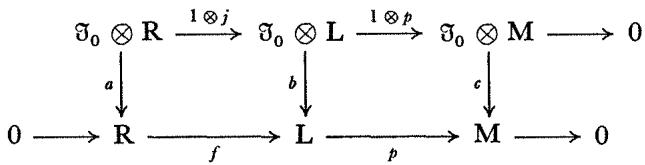
\includegraphics[keepaspectratio]{images/part003_24c814e1.jpg}}

where \(j\) is the canonical injection, \(a, b, c\) deriving from the canonical injection \(\mathfrak{I}_0 \to \mathbf{A}\) ( \(\S 3\) , no. 4, Proposition 4); it must be shown that \(a\) is surjective. Note that, as \(\mathbf{L}\) is free, \(b\) is injective ( \(\S 3\) , no. 7, Corollary 6 to Proposition 7) and \(c\) is injective by hypothesis. Then let \(t\) be an element of \(\mathbf{R}\) and \(t\) its class in \(\mathbf{R} / \mathfrak{I}_0\mathbf{R}\) ; then there is an exact sequence ( \(\S 3\) , no. 6, Proposition 5 and Corollary 2 to Proposition 6)

\[
\mathrm{R} / \mathfrak {I} _ {0} \mathrm{R} \xrightarrow {\jmath} \mathrm{L} / \mathfrak {I} _ {0} \mathrm{L} \xrightarrow {\bar {p}} \mathrm{M} / \mathfrak {I} _ {0} \mathrm{M} \longrightarrow 0
\]

where \(j\) and \(\bar{p}\) derive from \(j\) and \(p\) when passing to the quotients and \(\bar{p}\) is by hypothesis a bijection; then \(\bar{j}(t) = 0\) , in other words \(j(t) \in \mathfrak{I}_0\mathbf{L}\) . Then there is an element \(z \in \mathfrak{I}_0 \otimes \mathbf{L}\) such that \(j(t) = b(z)\) ; as \(p(b(z)) = 0\) , \(c((1 \otimes p)(z)) = 0\) and, as \(c\) is injective, \((1 \otimes p)(z) = 0\) . In other words, \(z\) is the image of an element \(t' \in \mathfrak{I}_0 \otimes \mathbf{R}\) under \(1 \otimes j\) and then \(j(a(t')) = b(z) = j(t)\) ; as \(j\) is injective, this implies \(t = a(t')\) .

We shall show later (Commutative Algebra, II, § 3, no. 2, Proposition 5) how this proposition can be extended to non-graded modules.

Lemma 1. For a commutative group \(\Delta\) to be such that there exists on \(\Delta\) a total ordering compatible with the group structure of \(\Delta\) , it is necessary and sufficient that \(\Delta\) be torsion-free.

If there exists such an order structure on \(\Delta\) and if \(\lambda > 0\) , then \(\lambda + \mu > 0\) for all \(\mu \geqslant 0\) and in particular, by induction on the integer \(n > 0\) , \(n.\lambda > 0\) , which proves that \(\Delta\) is torsion-free (since every element \(\neq 0\) of \(\Delta\) is either \(>0\) or \(< 0\) ). Conversely, if \(\Delta\) is torsion-free, \(\Delta\) is a sub- \(\mathbf{Z}\) -module of a vector \(\mathbf{Q}\) -space ( \(\S 7\) , no. 10, Corollary 1 to Proposition 26) which may be assumed of the form \(\mathbf{Q}^{(I)}\) ; if I is given a well-ordering (Set Theory, III, \(\S 2\) , no. 3, Theorem 1) and \(\mathbf{Q}\) its usual ordering, the set \(\mathbf{Q}^{(I)}\) with the lexicographical ordering is totally ordered (Set Theory, III, \(\S 2\) , no. 6); it is immediate that this ordering is compatible with the additive group structure of \(\mathbf{Q}^{(I)}\) .

PROPOSITION 8. Let \(\Delta\) be a torsion-free commutative group and A a graded ring of type \(\Delta\) . If the product in A of two homogeneous elements \(\neq 0\) is \(\neq 0\) , the ring A has no divisor of 0.

Let \(\Delta\) be given a total ordering compatible with its group structure (Lemma

\begin{enumerate}
\def\labelenumi{\arabic{enumi})}
\tightlist
\item
  and let \(x = \sum_{\lambda \in \Delta} x_{\lambda}, y = \sum_{\lambda \in \Delta} y_{\lambda}\) be two non-zero elements of A ( \(x_{\lambda}\) and \(y_{\lambda}\) being homogeneous of degree \(\lambda\) for all \(\lambda \in \Delta\) ); let \(\alpha\) (resp. \(\beta\) ) be the greatest of the elements \(\lambda \in \Delta\) such that \(x_{\lambda} \neq 0\) (resp. \(y_{\lambda} \neq 0\) ); it is immediate that if \(\lambda \neq \alpha\) or \(\mu \neq \beta\) , either \(x_{\lambda}y_{\mu} = 0\) or \(\deg(x_{\lambda}y_{\mu}) < \alpha + \beta\) ; the homogeneous component of \(xy\) of degree \(\alpha + \beta\) is therefore \(x_{\alpha}y_{\beta}\) , which is non-zero by hypothesis; whence \(xy \neq 0\) .
\end{enumerate}

\subsection{GRADED TENSOR PRODUCT OF GRADED MODULES}

Let \(\Delta\) be a commutative monoid with its identity element denoted by 0, A a graded ring of type \(\Delta\) and M (resp. N) a graded right (resp. left) A-module of type \(\Delta\) . Let \((\mathbf{A}_{\lambda})\) (resp. \((\mathbf{M}_{\lambda}), (\mathbf{N}_{\lambda}))\) be the graduation of A (resp. M, N); the tensor product \(\mathbf{M} \otimes_{\mathbf{Z}} \mathbf{N}\) of the Z-modules M and N is the direct sum of the \(\mathbf{M}_{\lambda} \otimes_{\mathbf{Z}} \mathbf{N}_{\mu}\) (§ 3, no. 7, Proposition 7) and hence the latter form a bigraduation of types \(\Delta, \Delta\) on this Z-module. Consider on M \(\otimes_{\mathbf{Z}} \mathbf{N}\) the total graduation of type \(\Delta\) associated with this bigraduation (no. 1, Example 4); it consists of the sub-Z-modules \(\mathrm{P}_{\lambda} = \sum_{\mu + v = \lambda} (\mathrm{M}_{\mu} \otimes_{\mathbf{z}} \mathrm{N}_{v})\) . It is known that the Z-module M \(\otimes_{\mathbf{A}} \mathbf{N}\) is the quotient of M \(\otimes_{\mathbf{Z}} \mathbf{N}\) by the sub-Z-module Q generated by the elements \((xa) \otimes y - x \otimes (ay)\) , where \(x \in \mathbf{M}, y \in \mathbf{N}\) and \(a \in \mathbf{A}\) (§ 3, no. 1); if, for all \(\lambda \in \Delta\) , \(x_{\lambda}, y_{\lambda}, a_{\lambda}\) are the homogeneous components of degree \(\lambda\) of \(x, y, a\) respectively, clearly \((xa) \otimes y - x \otimes (zy)\) is the sum of the homogeneous elements \((x_{\lambda}a_{v}) \otimes y_{\mu} - x_{\lambda} \otimes (a_{v}y_{\mu})\) , in other words Q is a graded sub-Z-module of M \(\otimes_{\mathbf{Z}} \mathbf{N}\) (no. 3, Proposition 2) and the quotient

\[
\mathbf {M} \otimes_ {\mathbf {A}} \mathbf {N} = (\mathbf {M} \otimes_ {\mathbf {Z}} \mathbf {N}) / \mathbf {Q}
\]

therefore has canonically a graded Z-module structure of type \(\Delta\) (no. 3). Moreover (no. 3, Proposition 5), the centre C of A is a graded subring of A; the graduation which we have just defined on M \(\otimes_{\mathbf{A}} \mathbf{N}\) is compatible with its module structure over the graded ring C. For M \(\otimes_{\mathbf{Z}} \mathbf{N}\) has canonically two C-module structures, for which respectively \(c(x \otimes y) = (xc) \otimes y\) and \((x \otimes y)c = x \otimes (cy)\) for \(x \in \mathbf{M}, y \in \mathbf{N}, c \in \mathbf{C}\) ( \(\S 3\) , no. 3); if \(x \in \mathbf{M}_{\lambda}, y \in \mathbf{N}_{\mu}, c \in \mathbf{C} \cap \mathbf{A}_{\nu}\) , the two elements \(c(x \otimes y)\) and \((x \otimes y)c\) belong to (M \(\otimes_{\mathbf{Z}} \mathbf{N})_{\lambda + \mu + \nu}\) and their difference belongs to Q and hence their common image in M \(\otimes_{\mathbf{A}} \mathbf{N}\) belongs to (M \(\otimes_{\mathbf{A}} \mathbf{N})_{\lambda + \mu + \nu}\) , which establishes our assertion. When we speak of M \(\otimes_{\mathbf{A}} \mathbf{N}\) as a graded C-module, we always mean with the structure thus defined, unless otherwise mentioned. Note that (M \(\otimes_{\mathbf{A}} \mathbf{N})_{\lambda}\) can be defined as the additive group of M \(\otimes_{\mathbf{A}} \mathbf{N}\) generated by the \(x_{\mu} \otimes y_{\nu}\) , where \(x_{\mu} \in \mathbf{M}_{\mu}, y_{\nu} \in \mathbf{N}_{\nu}\) and \(\mu + \nu = \lambda\) .

Let \(\mathbf{M}'\) (resp. \(\mathbf{N}'\) ) be another graded right (resp. left) A-module and \(u: \mathbf{M} \to \mathbf{M}', v: \mathbf{N} \to \mathbf{N}'\) graded homomorphisms of respective degrees \(\alpha\) and \(\beta\) . Then it follows immediately from the above remark that \(u \otimes v\) is a graded (C-module) homomorphism of degree \(\alpha + \beta\) .

When A is commutative, a graduation (compatible with the A-module structure) is similarly defined on the tensor product of any finite number of graded A-modules; it is moreover immediate that the associativity isomorphisms such as \((\mathbf{M} \otimes \mathbf{N}) \otimes \mathbf{P} \to \mathbf{M} \otimes (\mathbf{N} \otimes \mathbf{P})\) (§ 3, no. 8, Proposition 8) are isomorphisms of graded modules.

Remark. When A has the trivial graduation (no. 1, Example 1), \((\mathbf{M} \otimes_{\mathbf{A}} \mathbf{N})_{\lambda}\) is then simply the direct sum of the sub-Y-modules \(\mathbf{M}_{\mu} \otimes_{\mathbf{A}} \mathbf{N}_{\nu}\) of \(\mathbf{M} \otimes_{\mathbf{A}} \mathbf{N}\) such that \(\mu + \nu = \lambda\) .

Let M (resp. N) be a graded right (resp. left) A-module of type \(\Delta\) , P a graded Z-module of type \(\Delta\) and let f be a Z-bilinear mapping of \(M \times N\) into P satisfying condition (1) of §3, no. 1, and such moreover that

\[
f (x _ {\lambda}, y _ {\mu}) \in \mathrm{P} _ {\lambda + \mu} \quad \text { for } x _ {\lambda} \in \mathrm{M} _ {\lambda}, y _ {\mu} \in \mathrm{N} _ {\mu}, \lambda , \mu \text { in } \Delta .
\]

Then \(f(x, y) = g(x \otimes y)\) , where \(g: \mathbf{M} \otimes_{\mathbf{A}} \mathbf{N} \to \mathbf{P}\) is a \(\mathbf{Z}\) -linear mapping (§ 3, no. 1, Proposition 1) and it follows from the above condition that \(g\) is a graded \(\mathbf{Z}\) -module homomorphism of degree 0.

Let B be another graded ring of type \(\Delta\) and \(\rho: A \to B\) a homomorphism of graded rings (no. 2); then \(\rho_*(B_d)\) is a graded right A-module of type \(\Delta\) . If E is a graded left A-module of type \(\Delta\) and \(\rho^*(B_d) \otimes_A E\) is given the graded Z-module structure of type \(\Delta\) defined above, the canonical left B-module structure ( \(\S\) 5, no. 1) is compatible with the graduation of

\[
\mathbf {E} _ {(\mathbf {B})} = \rho^ {*} (\mathbf {E}) = \rho_ {*} (\mathbf {B} _ {d}) \otimes_ {\mathbf {A}} \mathbf {E}.
\]

The graded B-module thus obtained is said to be obtained by extending the ring of scalars to B by means of \(\rho\) and when we speak of \(\mathrm{E}_{(\mathrm{B})}\) or \(\rho^{*}(\mathrm{E})\) as a graded B-module, we always mean this structure, unless otherwise mentioned.

\subsection{GRADED MODULES OF GRADED HOMOMORPHISMS}

We suppose in this no. that the monoid \(\Delta\) is a group. Let A be a graded ring of type \(\Delta\) and M, N two graded left (for example) A-modules of type \(\Delta\) . Let H \(_{\lambda}\) denote the additive group of graded homomorphisms of degree \(\lambda\) of M into N (no. 2); in the additive group Hom \(_{A}\) (M, N) of all homomorphisms of M into N (with the non-graded A-module structures) the sum (for \(\lambda \in \Delta\) ) of the H \(_{\lambda}\) is direct. For, if there is a relation \(\sum_{\lambda} u_{\lambda} = 0\) with \(u_{\lambda} \in \mathrm{H}_{\lambda}\) for all \(\lambda\) , it follows that \(\sum_{\lambda} u_{\lambda}(x_{\mu}) = 0\) for all \(\mu\) and all \(x_{\mu} \in \mathrm{M}_{\mu}\) . As the elements of \(\Delta\) are cancellable, \(u_{\lambda}(x_{\mu})\) is the homogeneous component of \(\sum_{\lambda} u_{\lambda}(x_{\mu})\) of degree \(\lambda + \mu\) ; hence \(u_{\lambda}(x_{\mu}) = 0\) for every ordered pair ( \(\mu, \lambda\) ) and every \(x_{\mu} \in \mathrm{M}_{\mu}\) , which implies \(u_{\lambda} = 0\) for all \(\lambda \in \Delta\) . We shall denote (in this paragraph) by Homgr \(_{A}\) (M, N) the additive subgroup of Hom \(_{A}\) (M, N) the sum of the H \(_{\lambda}\) and we shall call it the additive group of graded A-module homomorphisms of M into N. Let C be the centre of A, which is a graded subring (no. 3, Corollary to Proposition 5); for the canonical C-module structure on \(\mathrm{Hom}_{\mathbf{A}}(\mathbf{M},\mathbf{N})\) (§ 1, no. 14, Remark 1), \(\mathrm{Homgr}_{\mathbf{A}}(\mathbf{M},\mathbf{N})\) is a submodule and the graduation \((\mathbf{H}_{\lambda})\) is compatible with the C-module structure: for, if \(c_{\nu}\in \mathbf{C}\cap \mathbf{A}_{\nu}\) , \(x_{\mu}\in \mathbf{N}_{\mu}\) and \(u_{\lambda}\in \mathbf{H}_{\lambda}\) , then by definition \((c_{\nu}u_{\lambda})(x_{\mu}) = c_{\nu}.u_{\lambda}(x_{\mu})\subset \mathbf{N}_{\lambda +\mu +\nu}\) and hence \(c_{\nu}u_{\lambda}\in \mathbf{H}_{\lambda +\nu}\) .

Let \(\mathbf{M}'\) and \(\mathbf{N}'\) be two graded left A-modules of type \(\Delta\) and \(u':\mathbf{M}'\to\mathbf{M}\) , \(v':\mathbf{N}\to\mathbf{N}'\) graded homomorphisms of respective degrees \(\alpha\) and \(\beta\) . Then it is immediate that \(\operatorname{Hom}(u',v')\colon w\mapsto v'\circ w\circ u'\) maps \(\operatorname{Homgr}_{\mathbf{A}}(\mathbf{M},\mathbf{N})\) into \(\operatorname{Homgr}_{\mathbf{A}}(\mathbf{M}',\mathbf{N}')\) and that its restriction to \(\operatorname{Homgr}_{\mathbf{A}}(\mathbf{M},\mathbf{N})\) is a graded homomorphism into \(\operatorname{Homgr}_{\mathbf{A}}(\mathbf{M}',\mathbf{N}')\) of degree \(\alpha+\beta\) .

In particular \(\operatorname{Homgr}_{\mathbf{A}}(\mathbf{M}, \mathbf{M})\) is a graded subring of \(\operatorname{End}_{\mathbf{A}}(\mathbf{M})\) , which is denoted by \(\operatorname{Endgr}_{\mathbf{A}}(\mathbf{M})\) .

Remark. If M and N are graded left A-modules, \(\operatorname{Homgr}_{\mathbf{A}}(\mathbf{M}, \mathbf{N})\) is in general distinct from \(\operatorname{Hom}_{\mathbf{A}}(\mathbf{M}, \mathbf{N})\) . However these two sets are equal when M is a finitely generated A-module. For M is then generated by a finite number of homogeneous elements \(x_{i}\) ( \(1 \leqslant i \leqslant n\) ); let \(d(i)\) be the degree of \(x_{i}\) ; let \(u \in \operatorname{Hom}_{\mathbf{A}}(\mathbf{M}, \mathbf{N})\) and for all \(\lambda \in \Delta\) let \(z_{i,\lambda}\) denote the homogeneous component of \(u(x_{i})\) of degree \(\lambda + d(i)\) . We show that there exists a homomorphism \(u_{\lambda}: \mathbf{M} \to \mathbf{N}\) such that \(u_{\lambda}(x_{i}) = z_{i,\lambda}\) for all \(i\) . It suffices to prove that if \(\sum_{i} a_{i} x_{i} = 0\) with \(a_{i} \in \mathbf{A}\) for \(1 \leqslant i \leqslant n\) , then \(\sum_{i} a_{i} z_{i,\lambda} = 0\) for all \(\lambda \in \Delta\) (§ 1, no. 7, Remark). It can be assumed that each \(a_{i}\) is homogeneous of degree \(d'(i)\) such that \(d(i) + d'(i) = \mu\) for all \(i\) (no. 3, Remark 1); then \(\sum_{i} a_{i} u(x_{i}) = 0\) ; taking the homogeneous component of degree \(\lambda + \mu\) on the left-hand side, we obtain \(\sum_{i} a_{i} z_{i,\lambda} = 0\) , whence the existence of the homomorphism \(u_{\lambda}\) ; clearly moreover \(u_{\lambda}\) is graded of degree \(\lambda\) . Finally, \(u_{\lambda} = 0\) except for a finite number of values of \(\lambda\) , and \(u = \sum_{\lambda} u_{\lambda}\) by definition, which proves our assertion.

In particular, \(\operatorname{Homgr}_{\mathbf{A}}(\mathbf{A}_s, \mathbf{M}) = \operatorname{Hom}_{\mathbf{A}}(\mathbf{A}_s, \mathbf{M})\) for every graded left A-module M; moreover \(\operatorname{Hom}_{\mathbf{A}}(\mathbf{A}_s, \mathbf{M})\) has a graded left A-module structure (and not just a graded C-module structure), and it is immediate that with this structure the canonical mapping of M into \(\operatorname{Hom}_{\mathbf{A}}(\mathbf{A}_s, \mathbf{M})\) ( \(\S 1\) , no. 14, Remark 2) is a graded A-module isomorphism.

Similarly, \(\operatorname{Homgr}_{\mathbf{A}}(\mathbf{M}, \mathbf{A}_s)\) has a graded right A-module structure (and not only a graded C-module structure); it is called the graded dual of the graded A-module M and is denoted by \(\mathbf{M}^{*\mathbf{gr}}\) , or simply \(\mathbf{M}^*\) when no confusion results. If \(u: \mathbf{M} \to \mathbf{N}\) is a graded homomorphism of degree \(\delta\) , it follows from the above that the restriction to \(\mathbf{N}^{*\mathbf{gr}}\) of \(^t u = \operatorname{Hom}(u, 1_{\mathbf{A}_s})\) is a graded homomorphism of the graded dual \(\mathbf{N}^{*\mathbf{gr}}\) into the graded dual \(\mathbf{M}^{*\mathbf{gr}}\) , of degree \(\delta\) , called the graded transpose of \(u\) .

We sometimes consider on the graded dual \(M^{*gr}\) the graduation derived from the above with the aid of the isomorphism \(\lambda\mapsto-\lambda\) of \(\Delta\) (no. 1, Example 2) so that the homogeneous elements of degree \(\lambda\) in \(M^{*gr}\) are the graded linear forms of degree \(-\lambda\) on M (when A has the trivial graduation, these are the zero linear forms of the \(M_{\mu}\) of index \(\mu\neq\lambda\) ). Then, if \(u:M\to N\) is a graded homomorphism of degree \(\delta\) , \(u'\) becomes a graded homomorphism of degree \(-\delta\) .

Suppose A is commutative and graded of type \(\Delta\) and let M, N, P, Q be four graded A-modules of type \(\Delta\) . Then there are canonical graded homomorphisms of degree 0

\begin{enumerate}
\def\labelenumi{(\arabic{enumi})}
\setcounter{enumi}{2}
\tightlist
\item
\end{enumerate}

\[
\operatorname{Homgr} _ {\mathbf {A}} (\mathbf {M}, \operatorname{Homgr} _ {\mathbf {A}} (\mathbf {N}, \mathbf {P})) \rightarrow \operatorname{Homgr} _ {\mathbf {A}} (\mathbf {M} \otimes_ {\mathbf {A}} \mathbf {N}, \mathbf {P})\tag{4}
\]

\[
\operatorname{Homgr} _ {\mathbf {A}} (\mathbf {M}, \mathbf {N}) \otimes_ {\mathbf {A}} \mathrm{P} \rightarrow \operatorname{Homgr} _ {\mathbf {A}} (\mathbf {M}, \mathbf {N} \otimes_ {\mathbf {A}} \mathrm{P})
\]

\[
\operatorname{Homgr} _ {\mathbf {A}} (\mathbf {M}, \mathbf {P}) \otimes_ {\mathbf {A}} \operatorname{Homgr} _ {\mathbf {A}} (\mathbf {N}, \mathbf {Q}) \rightarrow \operatorname{Homgr} _ {\mathbf {A}} (\mathbf {M} \otimes_ {\mathbf {A}} \mathbf {N}, \mathbf {P} \otimes_ {\mathbf {A}} \mathbf {Q}) \tag {5}
\]

(the tensor products being given the graduations defined in no. 5) obtained by restricting the canonical homomorphisms defined in §4, nos. 1, 2 and 4; for, if \(u: \mathbf{M} \to \operatorname{Homgr}_{\mathbf{A}}(\mathbf{N}, \mathbf{P})\) is graded of degree \(\delta\) , then, for all \(x \in \mathbf{M}_{\lambda}\) , \(u(x)\) is a graded homomorphism \(\mathbf{N} \to \mathbf{P}\) of degree \(\delta + \lambda\) and hence, for \(y \in \mathbf{N}_{\mu}\) , \(u(x)(y) \in \mathbf{P}_{\delta + \lambda + \mu}\) ; if \(v: \mathbf{M} \otimes_{\mathbf{A}} \mathbf{N} \to \mathbf{P}\) corresponds canonically to \(u\) , it is then seen that \(v\) is a graded homomorphisms of degree \(\delta\) , whence our assertion concerning (3); moreover it is seen that this homomorphism is bijective. The argument is similar for (4) and (5).

If in particular \(\mathbf{P} = \mathbf{Q} = \mathbf{A}\) in (5), then there is a canonical graded homomorphism of degree 0

\[
\mathbf {M} ^ {* \mathrm{gr}} \otimes_ {\mathbf {A}} \mathbf {N} ^ {* \mathrm{gr}} \rightarrow (\mathbf {M} \otimes_ {\mathbf {A}} \mathbf {N}) ^ {* \mathrm{gr}}.\tag{6}
\]

\BourbakiAppendixSection{Pseudomodules}

\subsection{ADJUNCTION OF A UNIT ELEMENT TO A PSEUDO-RING}

Let A be a pseudo-ring (I, § 8, no. 1). On the set \(\mathbf{A}' = \mathbf{Z} \times \mathbf{A}\) we define the following laws of composition:

\[
\left\{ \begin{array}{l} (m, a) + (n, b) = (m + n, a + b) \\ (m, a) (n, b) = (m n, m b + n a + a b). \end{array} \right.\tag{1}
\]

It is immediately verified that A' with these two laws of composition is a ring in which the element \((1,0)\) is the unit element. The set \(\{0\} \times A\) is a two-sided ideal of A' and \(\iota: x \mapsto (0, x)\) is an isomorphism of the pseudo-ring A onto the sub-pseudo-ring \(\{0\} \times A\) by means of which A and \(\{0\} \times A\) are identified. A' is called the ring derived from the pseudo-ring A by adjoining a unit element.

If A already has an identity element \(\varepsilon\) , the element \(e = (0, \varepsilon)\) of \(\mathbf{A}'\) is an idempotent belonging to the centre of \(\mathbf{A}'\) and such that

\[
\mathrm{A} = e \mathrm{A} ^ {\prime} = \mathrm{A} ^ {\prime} e.
\]

Then \((e\mathbf{A}', (1 - e)\mathbf{A}')\) is a direct decomposition (I, § 8, no. 11) of \(\mathbf{A}'\) and the ring \((1 - e)\mathbf{A}'\) is isomorphic to \(\mathbf{Z}\) .

\subsection{PSEUDOMODULES}

Given a pseudo-ring A with or without a unit element, a left pseudomodule over A is a commutative group E (written additively) admitting A as set of operators and satisfying axioms \((\mathbf{M}_{\mathrm{I}})\) , \((\mathbf{M}_{\mathrm{II}})\) and \((\mathbf{M}_{\mathrm{III}})\) of §1, no. 1, Definition 1. Right pseudomodules over A are defined similarly.

Let \(A'\) be the ring obtained by adjoining a unit element to A. If E is a left pseudomodule over A, a left \(A'\) -module structure on E is associated with it by writing, for all \(x \in E\) and every element \((n, a) \in A'\) ,

\[
(n, a). x = n x + a x.\tag{2}
\]

Axioms \((\mathbf{M}_{\mathrm{I}})\) to \((\mathbf{M}_{\mathrm{IV}})\) of § 1, no. 1, Definition 1 are immediately verified; moreover, by restricting the set of operators of this module structure to \(\{0\} \times A\) (identified with A), we obtain on E the pseudomodule structure given initially.

For a subset M of E to be a subgroup with operators of the pseudomodule E (in which case the induced structure is obviously also a left pseudomodule structure over A), it is necessary and sufficient that M be a submodule of the associated A'-module E and this sub-A'-module is associated with the pseudomodule M. Moreover, the quotient A'-module E/M is then associated with the quotient group with operators E/M, which is obviously a pseudomodule over A.

If E, F are two pseudomodules over A, the homomorphisms \(E \rightarrow F\) of groups with operators are identical with the A'-linear mappings \(E \rightarrow F\) of the A'-modules associated respectively with the pseudomodules E and F. If \((\mathbf{E}_{t})_{t \in I}\) is a family of pseudomodules over A, the groups with operators \(\prod_{i\in I}E\) and \(\bigoplus_{i\in I}E_{i}\) are pseudomodules over A and the associated A'-modules are respectively the product and direct sum of the associated A'-modules \(E_{i}\) . There are analogous results for inverse and direct limits of pseudomodules. The theory of pseudomodules over A can thus be entirely reduced to that of A'-modules.

\BourbakiExercisesHeading

\BourbakiExercisesSection

\begin{enumerate}
\def\labelenumi{\arabic{enumi}.}
\item
  Let E, F be two A-modules and \(u: \mathbf{E} \to \mathbf{F}\) a linear mapping. Let M be a submodule of E, N a submodule of F, \(i: \mathbf{M} \to \mathbf{E}\) the canonical injection and \(q: \mathbf{F} \to \mathbf{F} / \mathbf{N}\) the canonical surjection. Show that \(u(\mathbf{M}) = \operatorname{Im}(u \circ i)\) and \(u^{-1}(\mathbf{N}) = \operatorname{Ker}(q \circ u)\) .
\item
  Let E be a left A-module; for every left ideal a of A let aE denote the sum of the ax where \(x \in E\) , which is therefore a submodule of E.
\end{enumerate}

\begin{enumerate}
\def\labelenumi{(\alph{enumi})}
\item
  Show that for every family \((\mathbf{E}_{\lambda})_{\lambda \in L}\) of A-modules, a. \(\bigoplus_{\lambda \in L} \mathbf{E}_{\lambda}\) is canonically identified with \(\bigoplus_{\lambda \in L} a E_{\lambda}\) .
\item
  If \(\mathfrak{a}\) is a finitely generated left ideal of \(\mathbf{A}\) , show that for every family \((\mathbf{E}_{\lambda})_{\lambda \in L}\) of \(\mathbf{A}\) -modules, \(\mathfrak{a}\) . \(\prod_{\lambda \in L} \mathbf{E}_{\lambda}\) is canonically identified with \(\prod_{\lambda \in L} \mathfrak{a}\mathbf{E}_{\lambda}\) . Give an example where \(\mathfrak{a}\) is not finitely generated and the above property fails to hold (take \(\mathbf{A}\) commutative and all the \(\mathbf{E}_{\lambda}\) equal to \(\mathbf{A}\) ).
\end{enumerate}

*(c) Let K be a commutative field, A the ring K{[}X,Y{]} of polynomials in two indeterminates over K, m = AX and n = AY. If E is the quotient A-module of \(\mathbf{A}^2\) by the submodule of \(\mathbf{A}^2\) generated by \(\mathbf{Xe}_1 - \mathbf{Ye}_2\) (where \((e_1, e_2)\) is the canonical basis of \(\mathbf{A}^2\) ), show that \((m \cap n)E \neq (mE) \cap (nE)\) .*

\begin{enumerate}
\def\labelenumi{\arabic{enumi}.}
\setcounter{enumi}{2}
\tightlist
\item
  Let E be an A-module.
\end{enumerate}

\begin{enumerate}
\def\labelenumi{(\alph{enumi})}
\tightlist
\item
  Let \((\mathbf{L}_{\mu})_{\mu \in \mathbf{M}}\) be a family of right directed ordered sets and, for all \(\mu \in \mathbf{M}\) , let \((\mathrm{F}_{\lambda \mu})_{\lambda \in L_{\mu}}\) be an increasing family of submodules of \(\mathbf{E}\) . Show that
\end{enumerate}

\[
\bigcap_ {\mu \in \mathbf {M}} \left(\sum_ {\lambda \in L _ {\mu}} F _ {\lambda \mu}\right) = \sum_ {\rho \in \prod_ {\mu} L _ {\mu}} \left(\bigcap_ {\mu \in \mathbf {M}} F _ {\rho (\mu), \mu}\right).
\]

\begin{enumerate}
\def\labelenumi{(\alph{enumi})}
\setcounter{enumi}{1}
\tightlist
\item
  Take A to be a field and E the A-module \(A^{N}\) ; let G be the submodule \(\mathbf{A}^{(\mathbf{N})}\) of E; on the other hand, for every finite subset H of N, let \(F_{H}\) be the submodule \(\prod_{n\in \mathbf{N}}\mathbf{M}_n\) of \(\mathbf{E}\) , where \(\mathbf{M}_n = \mathbf{A}\) for \(n\notin \mathrm{H}\) and \(\mathbf{M}_n = 0\) for \(n\in \mathrm{H}\) . Show that the family \((\mathrm{F_H})\) , where \(\mathbf{H}\) runs throughout the set \(\Phi\) of finite subsets of \(\mathbf{N}\) is right directed and that
\end{enumerate}

\[
\left(\bigcap_ {\mathrm{H} \in \Phi} \mathrm{F} _ {\mathrm{H}}\right) + \mathrm{G} \neq \bigcap_ {\mathrm{H} \in \Phi} (\mathrm{F} _ {\mathrm{H}} + \mathrm{G}).
\]

\begin{enumerate}
\def\labelenumi{\arabic{enumi}.}
\setcounter{enumi}{3}
\tightlist
\item
  Let \(\mathbf{E}, \mathbf{F}_1, \mathbf{F}_2\) be three A-modules and \(f_1: \mathbf{F}_1 \to \mathbf{E}\) , \(f_2: \mathbf{F}_2 \to \mathbf{E}\) two A-linear mappings. The fibre product of \(\mathbf{F}_1\) and \(\mathbf{F}_2\) relative to \(f_1\) and \(f_2\) is the submodule of the product \(\mathbf{F}_1 \times \mathbf{F}_2\) consisting of the ordered pairs \((x_1, x_2)\) such that \(f_1(x_1) = f_2(x_2)\) ; it is denoted by \(\mathbf{F}_1 \times_{\mathbf{E}} \mathbf{F}_2\) .
\end{enumerate}

\begin{enumerate}
\def\labelenumi{(\alph{enumi})}
\item
  For every ordered pair of A-linear mappings \(u_1 \colon G \to F_1, u_2 \colon G \to F_2\) such that \(f_1 \circ u_1 = f_2 \circ u_2\) , there exists one and only one A-linear mapping \(u \colon G \to F_1 \times_E F_2\) such that \(p_1 \circ u = u_1, p_2 \circ u = u_2\) , where \(p_1\) and \(p_2\) denote the restrictions to \(F_1 \times_E F_2\) of the projections \(pr_1\) and \(pr_2\) .
\item
  Let \(\mathbf{E}'\) , \(\mathbf{F}_1'\) , \(\mathbf{F}_2'\) be three A-modules, \(f_1': \mathbf{F}_1' \to \mathbf{E}', f_2': \mathbf{F}_2' \to \mathbf{E}'\) A-linear mappings and \(\mathbf{F}_1' \times_{\mathbf{E}'} \mathbf{F}_2'\) the fibre product relative to these mappings. For every system of A-linear mappings \(v_1: \mathbf{F}_1 \to \mathbf{F}_1'\) , \(v_2: \mathbf{F}_2 \to \mathbf{F}_2'\) , \(w: \mathbf{E} \to \mathbf{E}'\) such that \(f_1' \circ v_1 = w \circ f_1, f_2' \circ v_2 = w \circ f_2\) , let \(v\) be the A-linear mapping of \(\mathbf{F}_1 \times_{\mathbf{E}} \mathbf{F}_2\) into \(\mathbf{F}_1' \times_{\mathbf{E}'} \mathbf{F}_2'\) corresponding to the two linear mappings \(v_1 \circ p_1\) and \(v_2 \circ p_2\) . Show that if \(v_1\) and \(v_2\) are injective, so is \(v\) ; give an example where \(v_1\) and \(v_2\) are surjective but \(v\) is not surjective (take \(\mathbf{E}' = \{0\}\) ). If \(w\) is injective and \(v_1\) and \(v_2\) surjective, show that \(v\) is surjective.
\end{enumerate}

\begin{enumerate}
\def\labelenumi{\arabic{enumi}.}
\setcounter{enumi}{4}
\tightlist
\item
  Let \(\mathbf{E}, \mathbf{F}_1, \mathbf{F}_2\) be three A-modules and \(f_1: \mathbf{E} \to \mathbf{F}_1, f_2: \mathbf{E} \to \mathbf{F}_2\) two linear mappings. The amalgamated sum of \(\mathbf{F}_1\) and \(\mathbf{F}_2\) relative to \(f_1\) and \(f_2\) is the quotient module of \(\mathbf{F}_1 \times \mathbf{F}_2\) by the submodule the image of \(\mathbf{E}\) under the mapping \(z \mapsto (f_1(z), -f_2(z))\) ; it is denoted by \(\mathbf{F}_1 \oplus_{\mathbf{E}} \mathbf{F}_2\) .
\end{enumerate}

\begin{enumerate}
\def\labelenumi{(\alph{enumi})}
\tightlist
\item
  For every ordered pair of A-linear mappings \(u_{1}: \mathbf{F}_{1} \to \mathbf{G}, u_{2}: \mathbf{F}_{2} \to \mathbf{G}\) such that \(u_{1} \circ f_{1} = u_{2} \circ f_{2}\) , show that there exists one and only one A-linear mapping \(u: \mathbf{F}_{1} \oplus_{\mathbf{E}} \mathbf{F}_{2} \to \mathbf{G}\) such that \(u \circ j_{1} = u_{1}, u \circ j_{2} = u_{2}\) , where \(j_{1}\) and \(j_{2}\) denote the respective compositions of the canonical mapping
\end{enumerate}

\[
\mathbf {F} _ {1} \times \mathbf {F} _ {2} \rightarrow \mathbf {F} _ {1} \oplus_ {\mathrm{E}} \mathbf {F} _ {2}
\]

with the canonical injections \(\mathbf{F}_1\to \mathbf{F}_1\times \mathbf{F}_2,\mathbf{F}_2\rightarrow \mathbf{F}_1\times \mathbf{F}_2.\)

\begin{enumerate}
\def\labelenumi{(\alph{enumi})}
\setcounter{enumi}{1}
\tightlist
\item
  Let \(\mathbf{E}'\) , \(\mathbf{F}_1'\) , \(\mathbf{F}_2'\) be three A-modules, \(f_1': \mathbf{E}' \to \mathbf{F}_1'\) , \(f_2': \mathbf{E}' \to \mathbf{F}_2'\) two A-linear mappings and \(\mathbf{F}_1' \oplus_{\mathbf{E}'} \mathbf{F}_2'\) the amalgamated sum relative to these mappings. For every system of A-linear mappings \(v_1: \mathbf{F}_1' \to \mathbf{F}_1\) , \(v_2: \mathbf{F}_2' \to \mathbf{F}_2\) , \(w: \mathbf{E}' \to \mathbf{E}\) such that \(v_1 \circ f_1' = f_1 \circ w\) , \(v_2 \circ f_2' = f_2 \circ w\) , let \(v\) be the A-linear mapping of \(\mathbf{F}_1' \oplus_{\mathbf{E}'} \mathbf{F}_2'\) into \(\mathbf{F}_1 \oplus_{\mathbf{E}} \mathbf{F}_2\) corresponding to the two linear mappings \(j_1 \circ v_1\) and \(j_2 \circ v_2\) . Show that if \(v_1\) and \(v_2\) are surjective, so is \(v\) ; give an example where \(v_1\) and \(v_2\) are injective but \(v\) is not injective. Show that if \(w\) is surjective and \(v_1\) and \(v_2\) injective, then \(v\) is injective.
\end{enumerate}

\begin{enumerate}
\def\labelenumi{\arabic{enumi}.}
\setcounter{enumi}{5}
\tightlist
\item
  Given an A-module E, let \(\gamma(E)\) denote the least of the cardinals of the generating systems of E.
\end{enumerate}

\begin{enumerate}
\def\labelenumi{(\alph{enumi})}
\tightlist
\item
  If \(0 \to \mathbf{E} \to \mathbf{F} \to \mathbf{G} \to 0\) is an exact sequence of A-modules, then
\end{enumerate}

\[
\gamma (\mathbf {G}) \leqslant \gamma (\mathbf {F}) \leqslant \gamma (\mathbf {E}) + \gamma (\mathbf {G}).
\]

Give an example of a product \(\mathbf{F} = \mathbf{E} \times \mathbf{G}\) such that \(\gamma(\mathbf{E}) = \gamma(\mathbf{F}) = \gamma(\mathbf{G}) = 1\) (take \(\mathbf{E}\) and \(\mathbf{G}\) to be quotients of \(\mathbf{Z}\) ).

\begin{enumerate}
\def\labelenumi{(\alph{enumi})}
\setcounter{enumi}{1}
\item
  If \(\mathbf{E}\) is the sum of a family \((\mathrm{F}_{\lambda})_{\lambda \in L}\) of submodules, then \(\gamma (\mathbf{E})\leqslant \sum_{\lambda \in L}\gamma (\mathbf{F}_{\lambda}).\)
\item
  If \(\mathbf{M}\) and \(\mathbf{N}\) are submodules of a module \(\mathbf{E}\) , show that
\end{enumerate}

\[
\sup (\gamma (\mathbf {M}), \gamma (\mathbf {N})) \leqslant \gamma (\mathbf {M} \cap \mathbf {N}) + \gamma (\mathbf {M} + \mathbf {N}).
\]

\begin{enumerate}
\def\labelenumi{\arabic{enumi}.}
\setcounter{enumi}{6}
\tightlist
\item
  \begin{enumerate}
  \def\labelenumii{(\alph{enumii})}
  \tightlist
  \item
    Let A be a ring and E an (A, A)-bimodule; on the product \(B = A \times E\) a ring structure is defined by setting
  \end{enumerate}
\end{enumerate}

\[
(a, x) (a ^ {\prime}, x ^ {\prime}) = (a a ^ {\prime}, a x ^ {\prime} + x a ^ {\prime});
\]

E (canonically identified with \(\{0\} \times \mathbf{E}\) ) is then a two-sided ideal of B such that \(\mathbf{E}^2 = \{0\}\) .

\begin{enumerate}
\def\labelenumi{(\alph{enumi})}
\setcounter{enumi}{1}
\tightlist
\item
  By suitably choosing A and E, show that E can be a left B-module with \(\gamma(\mathbf{E})\) (Exercise 6) an arbitrary cardinal, although \(\gamma(\mathbf{B}_{s}) = 1\) .
\end{enumerate}

*8. Let A be a commutative ring, \(\mathbf{B} = \mathbf{A}[\mathbf{X}_n]_{n\geqslant 1}\) a polynomial ring over A in an infinity of indeterminates and C the quotient ring of B by the ideal generated by the polynomials \((\mathbf{X}_1 - \mathbf{X}_2)\mathbf{X}_i\) for \(i\geqslant 3\) . If \(\xi_1\) and \(\xi_2\) are the classes in C of \(\mathbf{X}_1\) and \(\mathbf{X}_2\) respectively, show that the intersection in C of the monogenous ideals \(\mathrm{C}\xi_1\) and \(\mathrm{C}\xi_2\) is not a finitely generated ideal.*

\begin{enumerate}
\def\labelenumi{\arabic{enumi}.}
\setcounter{enumi}{8}
\item
  Show that in an A-module E, if \((\mathrm{F}_{n})_{n\geqslant1}\) is a strictly increasing sequence of finitely generated submodules, the submodule F of E the union of the \(F_{n}\) is not finitely generated. Deduce that if E is an A-module which is not finitely generated, there exists a submodule F of E such that \(\gamma(\mathrm{F})=\aleph_{0}(=\mathrm{Card}(\mathbf{N}))\) .
\item
  Let E be a Z-module the direct sum of two submodules M, N respectively isomorphic to Z/2Z and Z/3Z; show that there exists no other decomposition of E as a direct sum of two non-zero submodules.
\item
  Let A be a ring admitting a field of left fractions (I, § 9, Exercise 15). Show that in the A-module \(A_{s}\) , a submodule distinct from \(A_{s}\) and \(\{0\}\) admits no supplementary submodule (cf.~I, § 9, Exercise 16).
\item
  Let \(\mathbf{G}\) be a module and \(\mathbf{E}, \mathbf{F}\) two submodules such that \(\mathbf{E} \subset \mathbf{F}\) .
\end{enumerate}

\begin{enumerate}
\def\labelenumi{(\alph{enumi})}
\item
  If F is a direct factor of G, F/E is a direct factor of G/E. If also E is a direct factor of F, E is a direct factor of G.
\item
  If E is a direct factor of G, then E is a direct factor of F. If also F/E is a direct factor of G/E, then F is a direct factor in G.
\item
  Give an example of two submodules \(\mathbf{M}, \mathbf{N}\) of the \(\mathbf{Z}\) -module \(\mathbf{E} = \mathbf{Z}^2\) such that \(\mathbf{M}\) and \(\mathbf{N}\) are direct factors of \(\mathbf{E}\) but \(\mathbf{M} + \mathbf{N}\) is not a direct factor of \(\mathbf{E}\) .
\item
  Let \(p\) be a prime number and \(U_p\) the submodule of the \(\mathbf{Z}\) -module \(\mathbf{Q} / \mathbf{Z}\) consisting of the classes mod \(\mathbf{Z}\) of rational numbers of the form \(k / p^n\) ( \(k \in \mathbf{Z}\) , \(n \in \mathbf{N}\) ). Let \(E\) be the product \(\mathbf{Z}\) -module \(M \times N\) , where \(M\) and \(N\) are both isomorphic to \(U_p\) , \(M\) and \(N\) being canonically identified with submodules of \(E\) . Consider the endomorphism \(u: (x, y) \mapsto (x, y + px)\) of \(E\) ; show that \(u\) is bijective. If \(M' = u(M)\) , show that \(M\) and \(M'\) are both direct factors of \(E\) but that \(M \cap M'\) is not a direct factor of \(E\) (use (b), showing that the \(Z\) -module \(U_p\) has no direct factor other than itself and \{0\}).
\end{enumerate}

¶ 13. Let E be an A-module and B the ring End\_A E. Show that for an element \(u \in B\) the following three conditions are equivalent: (1) Bu is a direct factor of the left B-module B\_s; (2) uB is a direct factor of the right B-module B\_d; (3) Ker(u) and Im(u) are direct factors of the A-module E. (Observe that every left ideal which is a direct factor of B\_s is of the form Bp, where p is a projector in E; cf.~I, § 8, Exercise 12 and use II, § 1, no. 9, Corollaries 1 and 2 to Proposition 15.)

\begin{enumerate}
\def\labelenumi{\arabic{enumi}.}
\setcounter{enumi}{13}
\tightlist
\item
  Let L be a well-ordered set, E an A-module and \((\mathbf{E}_{\lambda})_{\lambda \in L}\) an increasing family of submodules of E such that: (1) there exists a \(\lambda \in L\) such that \(E_{\lambda} = \{0\}\) ; (2) E is the union of the \(E_{\lambda}\) for \(\lambda \in L\) ; (3) if \(\lambda \in L\) is such that the set of \(\mu < \lambda\) admits a greatest element \(\lambda'\) , \(E_{\lambda}\) is the direct sum \(E_{\lambda'}\) and a submodule \(F_{\lambda}\) ; (4) if \(\lambda \in L\) is the least upper bound of the set of \(\mu < \lambda\) , then \(E_{\lambda}\) is the union of the \(E_{\mu}\) for \(\mu < \lambda\) . Under these conditions, show that E is the direct sum of the \(F_{\lambda}\) . (Prove by transfinite induction that each \(E_{\lambda}\) is the direct sum of the \(F_{\mu}\) such that \(\mu \leqslant \lambda\) .)
\end{enumerate}

¶ 15. Let c be an infinite cardinal.

\begin{enumerate}
\def\labelenumi{(\alph{enumi})}
\item
  Let I be a set and \(R\{a, b\}\) a relation between elements of I such that for all \(\alpha \in I\) the set of \(\beta \in I\) for which \(R\{\alpha, \beta\}\) holds has cardinal \(\leqslant c\) . Show that there exists a well-ordered set L and an increasing family \((\mathrm{I}_{\lambda})_{\lambda \in L}\) of subsets of I such that: (1) there exists a \(\lambda \in L\) such that \(I_{\lambda} = \varnothing\) ; (2) I is the union of the \(I_{\lambda}\) for \(\lambda \in L\) ; (3) if \(\lambda \in L\) is such that the set of \(\mu < \lambda\) has a greatest element \(\lambda'\) , \(\text{Card}(\mathbf{I}_{\lambda} - \mathbf{I}_{\lambda'}) \leqslant c\) ; (4) if \(\lambda \in L\) is the least upper bound of the set of \(\mu < \lambda\) , \(I_{\lambda}\) is the union of the \(I_{\mu}\) for \(\mu < \lambda\) ; (5) if \(\alpha \in I_{\lambda}\) and \(R\{\alpha, \beta\}\) holds, then \(\beta \in I_{\lambda}\) . (Note first that for all \(\alpha \in I\) the set of \(\beta \in I\) for which there exists an integer n and a sequence \((\gamma_{j})_{1 \leqslant j \leqslant n}\) of elements of I such that \(\gamma_{1} = \alpha, \gamma_{n} = \beta\) and \(R\{\gamma_{j}, \gamma_{j+1}\}\) holds for \(1 \leqslant j \leqslant n - 1\) , has cardinal \(\leqslant c\) . Then construct the \(I_{\lambda}\) by transfinite induction.)
\item
  Let E be an A-module the direct sum of a family \((\mathbf{M}_{\alpha})_{\alpha\in I}\) of submodules such that \(\gamma(\mathbf{M}_{\alpha})\leqslant c\) for all \(\alpha\in I\) (cf.~Exercise 6). Let f be an endomorphism of E. Show that there exists a well-ordered set L and an increasing family \((\mathbf{I}_{\lambda})_{\lambda\in L}\) of subsets of I satisfying properties (1), (2), (3) and (4) of (a) and such moreover that if we write \(\mathbf{E}_{\lambda} = \bigoplus_{\alpha \in \mathbf{I}_{\lambda}} \mathbf{M}_{\alpha}\) , then \(f(\mathbf{E}_{\lambda}) \subset \mathbf{E}_{\lambda}\) . (Apply (a) to the relation \(R\{\alpha, \beta\}\) : ``there exists \(x \in \mathbf{M}_{\alpha}\) such that the component of \(f(x)\) in \(\mathbf{M}_{\beta}\) is \(\neq 0\)''.) For all \(\lambda \in \mathbf{L}\) such that the set of \(\mu < \lambda\) has a greatest element \(\lambda'\) , write \(\mathbf{F}_{\lambda} = \bigoplus_{\alpha \in \mathbf{I}_{\lambda} - \mathbf{I}_{\lambda'}} \mathbf{M}_{\alpha}\) . Show that \(\mathbf{E}\) is the direct sum of the \(\mathbf{F}_{\lambda}\) (apply Exercise 14).
\item
  With the hypotheses and notation of (b), suppose further that \(f\) is a projector and write \(\mathbf{P} = f(\mathbf{E})\) . Let \(\mathbf{P}_{\lambda} = \mathbf{P} \cap \mathbf{E}_{\lambda}\) ; show that if \(\lambda \in \mathbf{L}\) is such that the set of \(\mu < \lambda\) has a greatest element \(\lambda'\) , \(\mathbf{P}_{\lambda'}\) is a direct factor of \(\mathbf{P}_{\lambda}\) (cf.~Exercise 12), that a supplementary submodule \(\mathbf{P}_{\lambda}'\) of \(\mathbf{P}_{\lambda'}\) in \(\mathbf{P}_{\lambda}\) is isomorphic to a direct factor of \(\mathbf{F}_{\lambda}\) and that \(\gamma(\mathbf{P}_{\lambda}') \leqslant c\) . Show that \(\mathbf{P}\) is the direct sum of the \(\mathbf{P}_{\lambda}'\) (apply Exercise 14).
\item
  Deduce from (c) that if an A-module E is the direct sum of a family \((\mathrm{M}_{\alpha})_{\alpha\in I}\) of submodules such that \(\gamma(\mathrm{M}_{\alpha})\leqslant\mathfrak{c}\) , then every direct factor P of E is also the direct sum of a family \((\mathrm{N}_{\lambda})_{\lambda\in L}\) of submodules such that \(\gamma(\mathrm{N}_{\lambda})\leqslant\mathfrak{c}\) .
\end{enumerate}

\begin{enumerate}
\def\labelenumi{\arabic{enumi}.}
\setcounter{enumi}{15}
\tightlist
\item
  Let A be a ring such that there exists an A-module M with a generating system of n elements but containing a free system of \(n + 1\) elements.
\end{enumerate}

\begin{enumerate}
\def\labelenumi{(\alph{enumi})}
\item
  Show that there exists in \(\mathbf{A}_s^n\) a free system of \(n + 1\) elements.
\item
  Deduce that there exists in M an infinite free system (construct such a system by induction using (a)).
\item
  Let C be a ring, E the free C-module \(\mathrm{C}_{s}^{(\mathrm{N})}, (e_{n})\) its canonical basis and A the endomorphism ring of E. Let \(u_{1}\) and \(u_{2}\) denote the endomorphisms of E defined by the conditions \(u_{1}(e_{2n}) = e_{n}, u_{1}(e_{2n+1}) = 0, u_{2}(e_{2n+1}) = e_{n}, u_{2}(e_{2n}) = 0\) for all \(n \geqslant 0\) . Show that \(u_{1}\) and \(u_{2}\) form a basis of the A-module \(A_{s}\) and deduce that in the A-module \(A_{s}\) there exist infinite free systems.
\end{enumerate}

*(d) Let A be the tensor algebra of a vector space E of dimension \(\geqslant 2\) over a commutative field (cf.~III, § 5, no. 1). Show that in the A-module \(A_s\) there exist infinite free systems (observe that two linearly independent vectors in E are linearly independent in \(A_s\) and use \((b)\) ). On the other hand, for every integer \(n > 0\) , every basis of the A-module \(A_s^n\) has \(n\) elements (cf.~§ 7, no. 2, Proposition 3).*

\begin{enumerate}
\def\labelenumi{\arabic{enumi}.}
\setcounter{enumi}{16}
\tightlist
\item
  Let A be a ring.
\end{enumerate}

\begin{enumerate}
\def\labelenumi{(\alph{enumi})}
\item
  Show that if the A-module \(\mathbf{A}_s^n\) is isomorphic to no \(\mathbf{A}_s^m\) for \(m > n\) , then, for all \(p < n\) , \(\mathbf{A}_s^p\) is isomorphic to no \(\mathbf{A}_s^q\) for \(q > p\) .
\item
  Show that if the A-module \(A_{s}^{n}\) contains no free system of \(n + 1\) elements, the A-module \(A_{s}^{p}\) contains no free system of \(p + 1\) elements for p \textless{} n.
\end{enumerate}

\begin{enumerate}
\def\labelenumi{\arabic{enumi}.}
\setcounter{enumi}{17}
\tightlist
\item
  Let A be a ring for which there exists an integer \(p\) with the following property: for every family \((a_i)_{1 \leqslant i \leqslant p}\) of \(p\) elements of A, there exists a family \((c_i)_{1 \leqslant i \leqslant p}\) of elements of A, one at least of which is not a right divisor of 0, such that \(\sum_{i=1}^{p} c_i a_i = 0\) .
\end{enumerate}

\begin{enumerate}
\def\labelenumi{(\alph{enumi})}
\item
  Show, by induction on \(n\) , that for every family \((x_{i})\) of \(p^n\) elements of \(A_s^n\) , there exists a family \((c_j)\) of \(p^n\) elements of \(A\) , one at least of which is not a right divisor of 0, such that \(\sum_{j} c_j x_j = 0\) .
\item
  Deduce from (a) and Exercise 16 that for all n \textgreater{} 0, the A-module \(A_{s}^{n}\) contains no free system of \(n + 1\) elements.
\end{enumerate}

\begin{enumerate}
\def\labelenumi{\arabic{enumi}.}
\setcounter{enumi}{18}
\tightlist
\item
  Let A be a non-zero ring with no divisors of zero.
\end{enumerate}

\begin{enumerate}
\def\labelenumi{(\alph{enumi})}
\item
  Show that for \(n > 1\) , the A-module \(\mathbf{A}_s^n\) is not monogenous.
\item
  Given an integer \(n \geqslant 1\) , for the A-module \(\mathbf{A}_s^n\) to contain no free system of \(n + 1\) elements, it is necessary that A admit a field of left fractions (I, §9, Exercise 15); conversely, if this condition is satisfied, \(\mathbf{A}_s^n\) contains a free system of \(n + 1\) elements for no integer \(n > 0\) . (Use Exercises 17 and 18 and I, §9, Exercise 16.)
\item
  Show that if every left ideal of A is monogenous, A admits a field of left fractions (use (a) and I, § 9, Exercise 16).
\end{enumerate}

\begin{enumerate}
\def\labelenumi{\arabic{enumi}.}
\setcounter{enumi}{19}
\tightlist
\item
  \begin{enumerate}
  \def\labelenumii{(\alph{enumii})}
  \tightlist
  \item
    Let A be a ring admitting a field of left fractions (I, § 9, Exercise 15). Let E be an A-module; show that, if in E \((x_{i})_{1\leqslant i\leqslant r}\) is a free system and \(y,z\) two elements such that \(x_{1},\ldots ,x_{r},y\) on the one hand and \(x_{1},\ldots ,x_{r},z\) on the other are two related systems, then \(x_{2},\ldots ,x_{r},y,z\) is a related system.
  \end{enumerate}
\end{enumerate}

\begin{enumerate}
\def\labelenumi{(\alph{enumi})}
\setcounter{enumi}{1}
\tightlist
\item
  Let A be the quotient ring Z/6Z and let \((e_{1}, e_{2})\) be the canonical basis of \(A^{2}\) ; show that if \(a = 2e_{1} + 3e_{2}\) , a and \(e_{1}\) form a related system, as do a and \(e_{2}\) , although \(e_{1}\) and \(e_{2}\) form a free system.
\end{enumerate}

\begin{enumerate}
\def\labelenumi{\arabic{enumi}.}
\setcounter{enumi}{20}
\item
  Let A be a ring, b, c two elements of A which are not right divisors of 0, M the A-module A/Abc and N the submodule Ac/Abc of M. For N to be a direct factor in M, it is necessary and sufficient that there exist two elements x, y of A such that \(xb + cy = 1\) . (If \(\varepsilon\) is the class of 1 in M, show that a supplementary subspace of N in M is generated by an element of the form \((1 - yc)\varepsilon\) whose annihilator is the ideal Ac.)
\item
  If an A-module E admits a basis whose indexing set is I and one of the two sets A, I is infinite, show that E is equipotent to \(A \times I\) .
\item
  \begin{enumerate}
  \def\labelenumii{(\alph{enumii})}
  \tightlist
  \item
    Let M, N be two subsets of an A-module E and m and n their annihilators; show that the annihilator of M ∩ N contains m + n and give an example where it is distinct from m + n.
  \end{enumerate}
\end{enumerate}

\begin{enumerate}
\def\labelenumi{(\alph{enumi})}
\setcounter{enumi}{1}
\item
  In a product module \(\prod_{i} \mathbf{E}_{i}\) , the annihilator of a subset \(\mathbf{F}\) is the intersection of the annihilators of its projections.
\item
  In a free A-module, the annihilator of an element \(\neq0\) contains only left divisors of 0 in A; in particular, if A is a ring with no divisors of 0, every element \(\neq0\) of a free module is free.
\end{enumerate}

\begin{enumerate}
\def\labelenumi{\arabic{enumi}.}
\setcounter{enumi}{23}
\tightlist
\item
  Let E be an A-module and M, N two submodules of E. The transporter of M into N, denoted by N:M, is the set of \(a \in A\) such that \(aM \subset N\) ; it is a two-sided ideal of A, equal to \(\text{Ann}((\mathbf{M} + \mathbf{N})/\mathbf{N})\) .
\end{enumerate}

\begin{enumerate}
\def\labelenumi{(\alph{enumi})}
\item
  Let A be a commutative ring, M an A-module, N a sub-module of M and x an element of M; show that \(N \cap Ax = (N:Ax)x\) .
\item
  Let A be a commutative ring and \(a, b\) two ideals of A. Show that \(a:b \supset a\) and that \((a:b)/a\) is an A-module isomorphic to \(\operatorname{Hom}(A/b, A/a)\) .
\end{enumerate}

\begin{enumerate}
\def\labelenumi{\arabic{enumi}.}
\setcounter{enumi}{24}
\item
  Let E, F be two A-modules and \(u: E \to F\) a linear mapping. Show that the mapping \((x, y) \mapsto (x, y - u(x))\) of the product module \(E \times F\) to itself is an automorphism of \(E \times F\) . Deduce that if there exists a linear mapping \(v: F \to E\) and an \(a \in E\) such that \(v(u(a)) = a\) , there exists an automorphism w of \(E \times F\) such that \(w(a, 0) = (0, u(a))\) .
\item
  Let E be a free A-module with a basis containing at least two elements.
\end{enumerate}

\begin{enumerate}
\def\labelenumi{(\alph{enumi})}
\item
  Show that every semi-linear mapping of E into itself (relative to an automorphism of A) which permutes with all the automorphisms of E, is necessarily a homothety \(x \mapsto \alpha x (\alpha \in \mathbf{A})\) .
\item
  Deduce from (a) that the centre of \(\operatorname{End}_{\mathbf{A}}(\mathbf{E})\) is the ring of central homotheties, isomorphic to the centre of A.
\item
  Deduce from (a) that the centre of the group \(\mathbf{GL}(\mathbf{E})\) is the group of invertible central homotheties of E, which is isomorphic to the multiplicative group of invertible elements of the centre of A.
\end{enumerate}

\begin{enumerate}
\def\labelenumi{\arabic{enumi}.}
\setcounter{enumi}{26}
\tightlist
\item
  Let A be a commutative ring. Show that if an ideal \(\mathfrak{J}\) of A is a free A-module, then \(\mathfrak{J}\) is a monogenous A-module (in other words a principal ideal). Give an example showing that the proposition does not extend to the left ideals in a non-commutative ring (Exercise 16).
\end{enumerate}

\BourbakiExercisesSection

\begin{enumerate}
\def\labelenumi{\arabic{enumi}.}
\tightlist
\item
  \begin{enumerate}
  \def\labelenumii{(\alph{enumii})}
  \tightlist
  \item
    If A is a ring with no divisors of zero, show that every element \(\neq0\) of a projective A-module is free.
  \end{enumerate}
\end{enumerate}

\begin{enumerate}
\def\labelenumi{(\alph{enumi})}
\setcounter{enumi}{1}
\item
  Give an example of a projective A-module whose annihilator is non-zero (cf.~I, § 8, no. 11).
\item
  Show that the Z-module Q is not a projective Z-module. *(See Commutative Algebra, II, § 5, Exercise 11 for an example of a finitely generated projective module over an integral domain, which is not free.)*
\end{enumerate}

\begin{enumerate}
\def\labelenumi{\arabic{enumi}.}
\setcounter{enumi}{1}
\item
  Show that every projective A-module is the direct sum of a family of projective submodules each of which admits a countable number of generators (``Kaplansky's Theorem''; apply Exercise 15 of §1, to the case where E is a free module).
\item
  Let \(\mathfrak{c}\) be a cardinal and \(\mathbf{P}\) a projective A-module such that \(\gamma(\mathbf{P}) \leqslant \mathfrak{c}\) (§ 1,
\end{enumerate}

Exercise 6). Show that if L is a free A-module with an infinite basis of cardinal \(\geqslant c\) , P ⊕ L is isomorphic to L. (Observe that there exists a free A-module M, whose basis has cardinal \(\leqslant c\) , isomorphic to the direct sum of P and an A-module Q. Note that M \(^{(N)}\) and P ⊕ M \(^{(N)}\) are isomorphic.)

¶ 4. (a) Let E, E' be two A-modules, N a submodule of E and N' a submodule of E' such that E is projective and E/N and E'/N' are isomorphic. Show that there exists an exact sequence

\[
0 \longrightarrow \mathrm{N} \stackrel {u} {\longrightarrow} \mathrm{E} \oplus \mathrm{N} ^ {\prime} \stackrel {v} {\longrightarrow} \mathrm{E} ^ {\prime} \longrightarrow 0.
\]

(Observe that there exists a homomorphism \(f \colon \mathbf{E} \to \mathbf{E}'\) such that \(f(\mathbf{N}) \subset \mathbf{N}'\) , which gives when passing to the quotients an isomorphism \(\mathbf{E} / \mathbf{N} \to \mathbf{E}' / \mathbf{N}'\) ; define \(u\) and \(v\) in an analogous way to that used for the exact sequence (29) of §1, no. 7.)

\begin{enumerate}
\def\labelenumi{(\alph{enumi})}
\setcounter{enumi}{1}
\item
  Deduce from (a) that if \(\mathbf{E}'\) is projective, \(\mathbf{E} \oplus \mathbf{N}'\) and \(\mathbf{E}' \oplus \mathbf{N}\) are isomorphic.
\item
  Let \(0 \to \mathbf{E}_m \to \mathbf{E}_{m-1} \to \ldots \to \mathbf{E}_1 \to \mathbf{E}_0 \to 0\) be an exact sequence of A-modules such that \(\mathbf{E}_0, \mathbf{E}_1, \ldots, \mathbf{E}_{m-2}\) are projective. Show that the A-modules \(\bigoplus_{h \geqslant 0} \mathbf{E}_{m-2h}\) and \(\bigoplus_{h \geqslant 0} \mathbf{E}_{m-2h+1}\) are isomorphic (with the convention that \(\mathbf{E}_i = \{0\}\) for \(i < 0\) ).
\end{enumerate}

\begin{enumerate}
\def\labelenumi{\arabic{enumi}.}
\setcounter{enumi}{4}
\item
  Let \(u\) be a linear mapping from an A-module \(\mathbf{E}\) to an A-module \(\mathbf{F}\) and \(v = {}^t u\) its transpose. For every submodule \(\mathbf{N}'\) of \(\mathbf{F}^*\) , the submodule of \(\mathbf{E}\) orthogonal to \(v(\mathbf{N}')\) is \(\overline{u}^{-1}(\mathbf{N})\) , where \(\mathbf{N}\) is the submodule of \(\mathbf{F}\) orthogonal to \(\mathbf{N}'\) .
\item
  \begin{enumerate}
  \def\labelenumii{(\alph{enumii})}
  \tightlist
  \item
    If E is an A-module, every injective endomorphism u of E is not a left divisor of zero in the ring \(\operatorname{End}_{\mathbf{A}}(\mathbf{E})\) . Conversely, if for every sub-A-module \(F \neq \{0\}\) of E there exists an endomorphism \(v \neq 0\) of E such that \(v(\mathbf{E}) \subset \mathbf{F}\) , an element which is not a left divisor of zero in \(\operatorname{End}_{\mathbf{A}}(\mathbf{E})\) is an injective endomorphism. The above condition is satisfied if there exists a linear form \(x' \in E^*\) and an \(x \in E\) such that \(\langle x, x' \rangle\) is invertible in A and in particular if E is free.
  \end{enumerate}
\end{enumerate}

\begin{enumerate}
\def\labelenumi{(\alph{enumi})}
\setcounter{enumi}{1}
\item
  Every endomorphism \(\neq 0\) of the \(\mathbf{Z}\) -module \(\mathbf{Q}\) is bijective, although there exists no linear form \(\neq 0\) on \(\mathbf{Q}\) .
\item
  Let \(U_{p}\) be the Z-module defined in §1, Exercise 12(d). Show that the endomorphism \(x \mapsto px\) of \(U_{p}\) is not injective and is not a left divisor of zero in \(\operatorname{End}_{\mathbf{Z}}(\mathbf{U}_{p})\) .
\end{enumerate}

\begin{enumerate}
\def\labelenumi{\arabic{enumi}.}
\setcounter{enumi}{6}
\tightlist
\item
  \begin{enumerate}
  \def\labelenumii{(\alph{enumii})}
  \tightlist
  \item
    If \(u\) is a surjective endomorphism of an A-module \(\mathbf{E}\) , \(u\) is not a right divisor of zero in \(\operatorname{End}_{\mathbf{A}}(\mathbf{E})\) . Conversely, if for every submodule \(\mathbf{F} \neq \mathbf{E}\) of \(\mathbf{E}\) there exists a linear form \(x^{*} \in \mathbf{E}^{*}\) which is zero on \(\mathbf{F}\) and surjective, every element of \(\operatorname{End}_{\mathbf{A}}(\mathbf{E})\) which is not a right divisor of zero is a surjective endomorphism.
  \end{enumerate}
\end{enumerate}

\begin{enumerate}
\def\labelenumi{(\alph{enumi})}
\setcounter{enumi}{1}
\item
  If E is the Z-module defined in Exercise 6(c), show that every endomorphism \(\neq 0\) of E is surjective, although there exists no linear form \(\neq 0\) on E.
\item
  Show that if E is a free Z-module \(\neq0\) , there exist non-surjective endomorphisms of E which are not right divisors of 0 in \(\operatorname{End}_{\mathbf{Z}}(\mathbf{E})\) .
\end{enumerate}

\begin{enumerate}
\def\labelenumi{\arabic{enumi}.}
\setcounter{enumi}{7}
\tightlist
\item
  \begin{enumerate}
  \def\labelenumii{(\alph{enumii})}
  \tightlist
  \item
    Let E be a free A-module, F, G two A-modules and \(u: \mathbf{E} \to \mathbf{G}\) , \(v: \mathbf{F} \to \mathbf{G}\) two linear mappings. Show that if \(u(\mathbf{E}) \subset v(\mathbf{F})\) , there exists a linear mapping \(w: \mathbf{E} \to \mathbf{F}\) such that \(u = v \circ w\) .
  \end{enumerate}
\end{enumerate}

\begin{enumerate}
\def\labelenumi{(\alph{enumi})}
\setcounter{enumi}{1}
\item
  Give an example of two non-zero endomorphisms \(u, v\) of the \(\mathbf{Z}\) -module \(\mathbf{E}\) defined in Exercise 6(c) such that there exists no endomorphism \(w\) of \(\mathbf{E}\) for which \(u = v \circ w\) (although \(u(\mathbf{E}) = v(\mathbf{E}) = \mathbf{E}\) ).
\item
  Give an example of two endomorphisms \(u, v\) of the \(\mathbf{Z}\) -module \(\mathbf{Z}\) such that \(u^{-1}(0) = v^{-1}(0) = \{0\}\) , but such that there exists no endomorphism \(w\) of \(\mathbf{Z}\) for which \(u = w \circ v\) (cf.~§ 7, Exercise 14).
\end{enumerate}

\begin{enumerate}
\def\labelenumi{\arabic{enumi}.}
\setcounter{enumi}{8}
\tightlist
\item
  Given an A-module E, for every submodule M of E (resp. every submodule M' of E*), let M° (resp. M'°) denote the orthogonal of M in E* (resp. the orthogonal of M' in E). Consider the following four properties:
\end{enumerate}

\begin{enumerate}
\def\labelenumi{(\Alph{enumi})}
\item
  The canonical homomorphism \(c_{\mathbf{E}}: \mathbf{E} \to \mathbf{E}^{**}\) is bijective.
\item
  For every submodule M of E, the canonical homomorphism \(E^{*}/M^{\circ} \rightarrow M^{*}\) is bijective.
\item
  For every submodule M of E, \(M^{\circ\circ} = M\) .
\item
  For every ordered pair of submodules M, N of E,
\end{enumerate}

\[
(\mathbf {M} \cap \mathbf {N}) ^ {\circ} = \mathbf {M} ^ {\circ} + \mathbf {N} ^ {\circ}.
\]

\begin{enumerate}
\def\labelenumi{(\alph{enumi})}
\item
  Show that condition (B) implies (D) (prove that for \(x^{*} \in (\mathbf{M} \cap \mathbf{N})^{\circ}\) , there exists \(y^{*} \in \mathbf{E}^{*}\) such that \(\langle x + y, y^{*} \rangle = \langle x, x^{*} \rangle\) for \(x \in \mathbf{M}\) and \(y \in \mathbf{N}\) ).
\item
  Let A be a ring with no divisors of zero, but having no field of left fractions \(*\) (for example the tensor algebra of a vector space of dimension \textgreater1, cf.~III, § 5, Exercise 5) \(^{*}\) . If we take \(E = A_{s}\) , condition (A) is satisfied, but none of conditions (B), (C), (D) (for an example where (B), (C), (D) hold, but not (A), see § 7, no. 5, Theorem 6).
\item
  Take A to be a product ring \(\mathbf{K}^{\mathrm{I}}\) , where \(\mathbf{K}\) is a commutative field and I an infinite set. Show that the A-module \(\mathbf{E} = \mathbf{A}\) satisfies conditions (A) and (B), but not (C) (observe that the annihilators of the ideals of \(\mathbf{A}\) are all of the form \(\mathbf{K}^{\mathrm{J}}\) , where \(\mathbf{J} \subset \mathbf{I}\) ).
\item
  Suppose that for two submodules \(\mathbf{M},\mathbf{N}\) of \(\mathbf{E}\) such that \(\mathbf{N} \subset \mathbf{M}\) and \(\mathbf{N} \neq \mathbf{M}\) , the dual \((\mathbf{M} / \mathbf{N})^*\) is non-zero; then show that condition (B) implies (C).
\item
  The kernel of \(c_{\mathbf{E}}\) is the orthogonal \((\mathbf{E}^{*})^{\circ}\) of \(\mathbf{E}^{*}\) in \(\mathbf{E}\) . Give an example where neither \(\mathbf{E}^{*}\) nor \((\mathbf{E}^{*})^{\circ}\) is 0 (consider a module containing an element whose annihilator contains an element which is not a divisor of 0).
\item
  Let \(\mathbf{M}\) be a direct factor of \(\mathbf{E}\) ; show that \(\mathbf{M}^{\circ \circ} = \mathbf{M} + (\mathbf{E}^{*})^{\circ}\) .
\end{enumerate}

\begin{enumerate}
\def\labelenumi{\arabic{enumi}.}
\setcounter{enumi}{9}
\tightlist
\item
  Give an example of an A-linear mapping \(u: \mathbf{E} \to \mathbf{F}\) such that \(^t u\) is bijective but \(u\) is neither injective nor surjective (cf.~Exercise 6(b) and (c)).
\end{enumerate}

Deduce an example where \(y_{0} \in F\) is orthogonal to the kernel of \(^{t}u\) but where the equation \(u(x) = y_{0}\) has no solution.

¶ 11. Let A be a ring and I an A-module. I is called injective if, for every exact sequence \(\mathrm{E}' \to \mathrm{E} \to \mathrm{E}''\) of A-linear mappings, the sequence

\[
\operatorname{Hom} \left(\mathrm{E} ^ {\prime \prime}, \mathrm{I}\right)\rightarrow \operatorname{Hom} (\mathrm{E}, \mathrm{I}) \rightarrow \operatorname{Hom} \left(\mathrm{E} ^ {\prime}, \mathrm{I}\right)
\]

is exact.

\begin{enumerate}
\def\labelenumi{(\alph{enumi})}
\tightlist
\item
  Show that the following properties are equivalent:
\end{enumerate}

\((\alpha)\) I is injective.

(β) For every exact sequence \(0 \rightarrow E' \rightarrow E \rightarrow E'' \rightarrow 0\) of A-linear mappings, the sequence

\[
0 \rightarrow \operatorname{Hom} (\mathrm{E} ^ {\prime \prime}, \mathrm{I}) \rightarrow \operatorname{Hom} (\mathrm{E}, \mathrm{I}) \rightarrow \operatorname{Hom} (\mathrm{E} ^ {\prime}, \mathrm{I}) \rightarrow 0
\]

is exact.

(γ) For every A-module M and every submodule N of M, every A-linear mapping of N into I can be extended to an A-linear mapping of M into I.

(δ) For every left ideal \(\mathfrak{a}\) of A and every A-linear mapping \(f: \mathfrak{a} \to \mathbf{I}\) , there exists an element \(b \in \mathbf{I}\) such that \(f(a) = ab\) for all \(a \in \mathfrak{a}\) .

(ζ) I is a direct factor of every A-module containing it.

(θ) For every A-module E which is the sum of I and a monogenous submodule, I is a direct factor of E.

(To prove that (δ) implies (γ), show that property (δ) implies that if E is an A-module and F a submodule of E such that E/F is monogenous, then every linear mapping of F into I can be extended to a linear mapping of E into I. Then use Zorn's Lemma. To prove that (θ) implies (δ), consider the A-module \(A_{s} \times I = M\) , the submodule N of M consisting of the elements \((a, -f(a))\) for \(a \in \mathfrak{a}\) , and apply (θ) to the quotient module M/N.)

\begin{enumerate}
\def\labelenumi{(\alph{enumi})}
\setcounter{enumi}{1}
\tightlist
\item
  For a Z-module E to be injective, it is necessary and sufficient that for all \(x \in E\) and every integer \(n \neq 0\) , there exists \(y \in E\) such that ny = x. In particular, the Z-modules Q and Q/Z are injective.
\end{enumerate}

\begin{enumerate}
\def\labelenumi{\arabic{enumi}.}
\setcounter{enumi}{11}
\tightlist
\item
  \begin{enumerate}
  \def\labelenumii{(\alph{enumii})}
  \tightlist
  \item
    For a product \(\prod_{\lambda \in L} E_{\lambda}\) of A-modules to be injective (Exercise 11), it is necessary and sufficient that each of the \(E_{\lambda}\) be injective.
  \end{enumerate}
\end{enumerate}

\begin{enumerate}
\def\labelenumi{(\alph{enumi})}
\setcounter{enumi}{1}
\tightlist
\item
  Let K be a commutative field, L an infinite set and A the product ring \(K^{L}\) . Show that A is an injective A-module (use (a)) but that the ideal \(\mathfrak{a}\) of A the direct sum of the factors of \(K^{L}\) (canonically identified with ideals of A) is not an injective A-module.
\end{enumerate}

¶ 13. (a) Let A be a ring and I an injective A-module (Exercise 11) such that for every non-zero monogenous A-module E, there exists a non-zero A-homomorphism of E into I. Let M be an A-module, N a submodule of M and \(\tilde{\mathbf{N}}\) the set of \(u \in \operatorname{Hom}_{\mathbf{A}}(\mathbf{M}, \mathbf{I})\) such that \(u(x) = 0\) in N. Show that for all \(y \notin N\) , there exists a \(u \in \tilde{\mathbf{N}}\) such that \(u(y) \neq 0\) .

\begin{enumerate}
\def\labelenumi{(\alph{enumi})}
\setcounter{enumi}{1}
\item
  Let A be a ring. For every (A, A)-bimodule T and every left (resp. right) A-module M, \(\operatorname{Hom}_{\mathbf{A}}(\mathbf{M}, \mathbf{T})\) has canonically a right (resp. left) A-module structure deriving from that on T, and there is a canonical A-homomorphism \(c_{M,T}: M \to \operatorname{Hom}_{\mathbf{A}}(\operatorname{Hom}_{\mathbf{A}}(\mathbf{M}, \mathbf{T}), \mathbf{T})\) such that \(c_{M,T}(x)\) is the A-homomorphism \(u \mapsto u(x)\) . Show that if I is an (A, A)-bimodule which, as a left A-module, satisfies the conditions of (a), then the canonical homomorphism \(c_{M,I}\) is injective for every left A-module M.
\item
  Suppose that I is an (A, A)-bimodule which is injective as a left A-module and a right A-module and that for every (left or right) monogenous A-module \(E \neq 0\) , there exists a non-zero A-homomorphism of E into I. Show that under these conditions, if P is a left (resp. right) projective A-module, \(\operatorname{Hom}_{\mathbf{A}}(\mathbf{P}, \mathbf{I})\) is a right (resp. left) injective A-module. (Suppose that P is a left projective A-module. Observe that for every submodule \(N'\) of a right A-module N, \(\operatorname{Hom}_{\mathbf{A}}(\mathbf{N}', \mathbf{I})\) is isomorphic to a quotient module of \(\operatorname{Hom}_{\mathbf{A}}(\mathbf{N}, \mathbf{I})\) and apply (b) to the right module N and the left module P.)
\item
  Let C be a commutative ring, A a C-algebra and I an injective C-module such that for every monogenous C-module \(E \neq \{0\}\) there exists a non-zero C-homomorphism of E into I. For every A-module M, \(\operatorname{Hom}_{\mathbf{C}}(\mathbf{M}, \mathbf{I})\) is an A-module; show that for every projective A-module P, \(\operatorname{Hom}_{\mathbf{C}}(\mathbf{P}, \mathbf{I})\) is an injective A-module (same argument as in (c)).
\end{enumerate}

\begin{enumerate}
\def\labelenumi{\arabic{enumi}.}
\setcounter{enumi}{13}
\tightlist
\item
  Let A be a ring. Show that for every A-module M there exists an injective A-module I such that M is isomorphic to a submodule of I. (Apply Exercise 13(d) with C = Z, using Exercise 11(b) and the fact that every A-module is the quotient of a free A-module.)
\end{enumerate}

¶ 15. An A-module homomorphism \(u: \mathbf{E} \to \mathbf{F}\) is called essential if it is injective and if, for every submodule \(\mathbf{P} \neq \{0\}\) of \(\mathbf{F}\) , \(u^{-1}(\mathbf{P}) \neq \{0\}\) ; it suffices that this condition holds for every monogenous submodule \(\mathbf{P} \neq \{0\}\) of \(\mathbf{F}\) . If \(\mathbf{E}\) is a submodule of \(\mathbf{F}\) , \(\mathbf{F}\) is called an essential extension of \(\mathbf{E}\) if the canonical injection \(\mathbf{E} \to \mathbf{F}\) is essential.

\begin{enumerate}
\def\labelenumi{(\alph{enumi})}
\item
  Let \(u: \mathbf{E} \to \mathbf{F}\) , \(v: \mathbf{F} \to \mathbf{G}\) be two A-homomorphisms of A-modules. If \(u\) and \(v\) are essential, so is \(v \circ u\) . Conversely, if \(v \circ u\) is essential and \(v\) is injective, then \(u\) and \(v\) are essential.
\item
  Let E be a submodule of an A-module F and let \((\mathbf{F}_{\lambda})_{\lambda \in L}\) be a family of submodules of F containing E and whose union is F. Show that if each of the \(F_{\lambda}\) is an essential extension of E, so is F.
\item
  Let \((u_{\lambda})_{\lambda \in L}\) be a family of essential homomorphisms \(u_{\lambda} \colon \mathbf{E}_{\lambda} \to \mathbf{F}_{\lambda}\) . Show that the homomorphism \(\bigoplus_{\lambda \in L} u_{\lambda} \colon \bigoplus_{\lambda \in L} \mathbf{E}_{\lambda} \to \bigoplus_{\lambda \in L} \mathbf{F}_{\lambda}\) is essential. (Prove it first when \(L\) has two elements, then use (b).)
\item
  The \(\mathbf{Z}\) -module \(\mathbf{Q}\) is an essential extension of \(\mathbf{Z}\) but the product \(\mathbf{Q}^{\mathrm{N}}\) is not an essential extension of \(\mathbf{Z}^{\mathrm{N}}\) .
\item
  Let E be a submodule of a module F. Show that there exists a submodule
\end{enumerate}

Q of F such that \(Q \cap E = \{0\}\) and that the restriction to E of the canonical homomorphism \(F \to F/Q\) is essential.

\begin{enumerate}
\def\labelenumi{\arabic{enumi}.}
\setcounter{enumi}{15}
\tightlist
\item
  A submodule E of an A-module F is called irreducible with respect to F (or in F) if \(E \neq F\) and E is not the intersection of two submodules of F distinct from E.
\end{enumerate}

\begin{enumerate}
\def\labelenumi{(\alph{enumi})}
\item
  For an A-module F to be an essential extension of each of its submodules \(\neq \{0\}\) it is necessary and sufficient that \(\{0\}\) be irreducible with respect to F.
\item
  Let \((\mathbf{E}_{\lambda})_{\lambda \in L}\) be a family of submodules of an A-module \(\mathbf{F}\) . \((\mathbf{E}_{\lambda})_{\lambda \in L}\) is called a reduced irreducible decomposition of \(\{0\}\) in \(\mathbf{F}\) if each of the \(\mathbf{F}_{\lambda}\) is irreducible in \(\mathbf{F}\) , if the intersection of the \(\mathbf{E}_{\lambda}\) reduces to 0 and if none of the \(\mathbf{E}_{\lambda}\) contains the intersection of the \(\mathbf{E}_{\mu}\) for \(\mu \neq \lambda\) . When this is so, show that the canonical homomorphism of \(\mathbf{F}\) into \(\bigoplus_{\lambda \in L} (\mathbf{F} / \mathbf{E}_{\lambda})\) is essential (if \(\mathbf{E}_{\lambda}' = \bigcap_{\mu \neq \lambda} \mathbf{E}_{\mu}\) , observe that the image \(\mathbf{F}_{\lambda}'\) of \(\mathbf{E}_{\lambda}'\) in \(\mathbf{F} / \mathbf{E}_{\lambda}\) is non-zero and that the image of \(\mathbf{F}\) in \(\bigoplus_{\lambda \in L} (\mathbf{F} / \mathbf{E}_{\lambda})\) contains \(\bigoplus_{\lambda \in L} \mathbf{F}_{\lambda}'\) ; then apply Exercise 15(c)). Conversely, if \((\mathbf{E}_{\lambda})_{\lambda \in L}\) is a family of submodules of \(\mathbf{F}\) irreducible in \(\mathbf{F}\) and the canonical homomorphism \(\mathbf{F} \to \bigoplus_{\lambda \in L} (\mathbf{F} / \mathbf{E}_{\lambda})\) is essential, the family \((\mathbf{E}_{\lambda})\) is a reduced irreducible decomposition of \(\{0\}\) in \(\mathbf{F}\) .
\end{enumerate}

¶ 17. (a) Let M, N, M', N' be four submodules of a module E such that M ∩ N = M' ∩ N' = P. Show that

\[
\mathbf {M} = (\mathbf {M} + (\mathbf {N} \cap \mathbf {M} ^ {\prime})) \cap (\mathbf {M} + (\mathbf {N} \cap \mathbf {N} ^ {\prime})).
\]

Deduce that if \(\mathbf{M}\) is irreducible in \(\mathbf{E}\) , then necessarily \(\mathbf{P} = \mathbf{M}' \cap \mathbf{N}\) or \(\mathbf{P} = \mathbf{N}' \cap \mathbf{N}\) .

\begin{enumerate}
\def\labelenumi{(\alph{enumi})}
\setcounter{enumi}{1}
\tightlist
\item
  Let \((\mathrm{N}_{i})_{1\leqslant i\leqslant n}\) be a finite family of submodules of E irreducible in E and M its intersection. Show that if \((\mathrm{P}_{j})_{1\leqslant j\leqslant m}\) is a finite family of submodules of E such that \(M=\bigcap_{j}P_{j}\) , then for every index i such that \(1\leqslant i\leqslant n\) there exists an index \(\phi(i)\) such that \(1\leqslant\phi(i)\leqslant m\) and such that, if we write \(N_{i}^{\prime}=\bigcap_{k\neq i}N_{k}\) , then \(M=P_{\phi(i)}\cap N_{i}^{\prime}\) (use (a)). Deduce that if none of the \(P_{j}\) contains the intersection of the \(P_{k}\) of index \(\neq j\) , then \(m\leqslant n\) (successively replace the \(N_{i}\) by suitable \(P_{j}\) , using the above result). Conclude that two reduced irreducible decompositions of M in E, one of which is finite, necessarily have the same number of terms (cf.~Exercise 23).
\end{enumerate}

¶ 18. (a) For an A-module I to be injective, show that it is necessary and sufficient that I admit no essential extension distinct from itself (show that this condition implies condition (δ) of Exercise 11(a), arguing as for the proof that (θ) implies (δ) in that exercise).

\begin{enumerate}
\def\labelenumi{(\alph{enumi})}
\setcounter{enumi}{1}
\item
  Let I be an injective A-module. For a submodule E of I to be injective, it is necessary and sufficient that E admit no essential extension distinct from itself and contained in I (using Exercise 15(e)), show that this condition implies that E is a direct factor of I).
\item
  Let I be an injective A-module, E a submodule of I and \(h: \mathbf{E} \to \mathbf{F}\) an essential homomorphism. Show that there exists an injective homomorphism \(j: \mathbf{F} \to \mathbf{I}\) such that \(j \circ h\) is the canonical injection of E into I.
\item
  Let I be an A-module and E a submodule of I. Show that the following properties are equivalent:
\end{enumerate}

(α) I is injective and is an essential extension of E.

(β) I is injective and for every injective homomorphism \(j\) of \(E\) into an injective A-module \(J\) , there exists an injective homomorphism of \(I\) into \(J\) extending \(j\) .

(γ) I is injective and is the smallest injective submodule of I containing E.

(δ) I is an essential extension of E and for every essential homomorphism \(h: E \to F\) , there exists an injective homomorphism \(j: F \to I\) such that \(j \circ h\) is the canonical injection of E into I.

(Use (c) and (a).) When these equivalent conditions hold, I is called an injective envelope of E; I is then also an injective envelope of every submodule of I containing E.

\begin{enumerate}
\def\labelenumi{(\alph{enumi})}
\setcounter{enumi}{4}
\item
  Let I be an injective A-module and E a submodule of I. Show that every maximal element of the set of essential extensions of E contained in I is an injective envelope of E (use (b)). In particular, every A-module admits an injective envelope (cf.~Exercise 14).
\item
  If I, I' are two injective envelopes of the same A-module E, show that there exists an isomorphism of I onto I' leaving invariant the elements of E.
\end{enumerate}

¶ 19. (a) Let E, F be two A-modules and M an injective submodule of E ⊕ F. Let I be an injective envelope of M ∩ E in M and J a supplementary submodule of I in M. Show that the restriction to I (resp. J) of the canonical projection of E ⊕ F onto E (resp. F) is injective (compose with the projection of I into E an extension E → I of the injection M ∩ E → I).

\begin{enumerate}
\def\labelenumi{(\alph{enumi})}
\setcounter{enumi}{1}
\tightlist
\item
  Let E be an A-module and M a submodule of E, maximal in the set of injective submodules of E; M admits in E a supplementary submodule N which contains no injective submodule \(\neq\{0\}\) . Show that for every injective submodule P of E, the image of P under the projection of E onto M (under the decomposition of E as a direct sum \(M \oplus N\) ) is an injective envelope of \(P \cap M\) in M (use (a)). If \(M'\) is another submodule of E which is maximal in the set of injective submodules of E, show that there exists an automorphism of E transforming M into \(M'\) and leaving invariant the elements of N.
\end{enumerate}

¶ 20. (a) Let A be a ring admitting a field of left fractions K (I, § 9, Exercise 15). Show that K, considered as a left A-module, is an injective envelope of A \(_{s}\) . (Apply criterion (α) of Exercise 18(d) and criterion (δ) of Exercise 11(a) noting that if f: a → K is an A-linear mapping of a left ideal a of A into K, the element \(x^{-1}f(x)\) for \(x \in \mathfrak{a}, x \neq 0\) (the inverse being taken in K) does not depend on \(x \in \mathfrak{a}\) .)

\begin{enumerate}
\def\labelenumi{(\alph{enumi})}
\setcounter{enumi}{1}
\tightlist
\item
  Let \(U_{p}\) be the sub-Z-module of Q/Z consisting of the canonical images of the rational numbers of the form \(k/p^{n}\) , where p is a given prime number, \(k \in Z\) and \(n \in N\) (II, §1, Exercise 12(d)). Show that \(U_{p}\) is an injective envelope of each of the Z-modules \(p^{-n}Z/Z\) isomorphic to \(Z/p^{n}Z\) . Show that there exist automorphisms of \(U_{p}\) distinct from the identity automorphism leaving invariant the elements of a submodule \(p^{-n}Z/Z\) .
\end{enumerate}

¶ 21. (a) Let \((\mathbf{E}_j)_{j \in J}\) be a finite family of A-modules and for all \(j \in J\) let \(I_j\) be an injective envelope of \(E_j\) ; show that \(\bigoplus_{j \in J} I_j\) is an injective envelope of \(\bigoplus_{j \in J} E_j\) .

\begin{enumerate}
\def\labelenumi{(\alph{enumi})}
\setcounter{enumi}{1}
\tightlist
\item
  An A-module M is called indecomposable if it is distinct from \(\{0\}\) and it is not the direct sum of two submodules distinct from \(\{0\}\) . Show that if I is an injective A-module, the following properties are equivalent:
\end{enumerate}

\((\alpha)\) \(\{0\}\) is an irreducible submodule in I.

(β) I is indecomposable.

(γ) I is an injective envelope of each of its submodules \(\neq0\) . (Use (a) and Exercise 18 (e).)

(δ) I is isomorphic to the injective envelope \(\mathrm{I}(\mathrm{A}/\mathrm{q})\) , where q is an irreducible left ideal of A.

Moreover, when this is so, for all \(x \neq 0\) in I, \(\operatorname{Ann}(x)\) is an irreducible left ideal of A and I is isomorphic to \(\operatorname{I}(\mathbf{A} / \operatorname{Ann}(x))\) .

Deduce that for the injective envelope of an A-module E to be indecomposable, it is necessary and sufficient that \(\{0\}\) be an irreducible submodule of E.

\begin{enumerate}
\def\labelenumi{(\alph{enumi})}
\setcounter{enumi}{2}
\item
  Give an example of an indecomposable Z-module E such that its injective envelope I(E) is decomposable (cf.~VII, § 3, Exercise 5).
\item
  Let E be an A-module, I an injective envelope of E and \(I = \bigoplus_{\lambda \in L} I_{\lambda}\) a decomposition of I as a direct sum of a finite family of indecomposable injective submodules; for all \(\lambda \in L\) let \(J_{\lambda} = \bigoplus_{\mu \neq \lambda} I_{\mu}\) and let \(N_{\lambda} = J_{\lambda} \cap E\) . Show that \((\mathrm{N}_{\lambda})_{\lambda \in L}\) is a reduced irreducible decomposition of \(\{0\}\) in E (Exercise 16 (b)) and that \(I_{\lambda}\) is an injective envelope of \(E/N_{\lambda}\) . Conversely, every reduced irreducible decomposition of \(\{0\}\) in E can be obtained by the above procedure uniquely up to isomorphism (use Exercise 16 (b)).
\end{enumerate}

\begin{enumerate}
\def\labelenumi{\arabic{enumi}.}
\setcounter{enumi}{21}
\tightlist
\item
  Let I be an injective A-module. If I is indecomposable, every injective endomorphism of I is an automorphism of I. Deduce that, for I to be indecomposable, it is necessary and sufficient that the non-invertible elements of the ring End(I) form a two-sided ideal of that ring.
\end{enumerate}

¶ 23. Let M be an A-module, the direct sum of a family (finite or otherwise) \((\mathbf{M}_{\lambda})_{\lambda \in L}\) of submodules such that for all \(\lambda \in L\) the non-invertible elements of \(\operatorname{End}(\mathbf{M}_{\lambda})\) form a two-sided ideal of this ring (which implies that \(\mathbf{M}_{\lambda}\) is indecomposable).

\begin{enumerate}
\def\labelenumi{(\alph{enumi})}
\item
  Let \(f, g\) be two endomorphisms of \(\mathbf{M}\) such that \(f + g = 1_{\mathbf{M}}\) . Show that for every finite sequence \((\lambda_k)_{1 \leqslant k \leqslant s}\) of distinct indices in \(\mathbf{L}\) there exists a family of submodules \(\mathbf{N}_k\) ( \(1 \leqslant k \leqslant s\) ) of \(\mathbf{M}\) such that for every \(k\) one of the endomorphisms \(f, g\) restricted to \(\mathbf{M}_{\lambda_{k}}\) is an isomorphism of this submodule onto \(\mathbf{N}_k\) and that \(\mathbf{M}\) is the direct sum of the \(\mathbf{N}_k\) ( \(1 \leqslant k \leqslant s\) ) and the \(\mathbf{M}_{\lambda}\) for \(\lambda\) distinct from \(\lambda_k\) . (Reduce it to the case \(s = 1\) ; if \(\pi_{\lambda}\) is the canonical projection of \(\mathbf{M}\) onto \(\mathbf{M}_{\lambda}\) corresponding to the decomposition as a direct sum of \(\mathbf{M}_{\lambda}\) and \(\bigoplus_{\mu \neq \lambda} \mathbf{M}_{\mu}\) , note that either \(\pi_{\lambda} \circ f\) or \(\pi_{\lambda} \circ g\) , restricted to \(\mathbf{M}_{\lambda}\) , is an automorphism of \(\mathbf{M}_{\lambda}\) .)
\item
  Let \(f\) be an idempotent endomorphism of \(\mathbf{M}\) . Show that there exists at least one index \(\lambda \in \mathbf{L}\) such that the restriction of \(f\) to \(\mathbf{M}_{\lambda}\) is an isomorphism of \(\mathbf{M}_{\lambda}\) onto \(f(\mathbf{M}_{\lambda})\) ; moreover \(f(\mathbf{M}_{\lambda})\) is a direct factor of \(\mathbf{M}\) . (If \(g = 1_{\mathbf{M}} - f\) , note that there exists a finite sequence of indices \((\lambda_k)_{1 \leqslant k \leqslant s}\) such that the intersection of \(\operatorname{Ker}(g)\) and the direct sum of the \(\mathbf{M}_{\lambda_k}\) is \(\neq \{0\}\) and use (a).)
\item
  Deduce from (b) that every indecomposable direct factor of M is isomorphic to one of the \(M_{\lambda}\) .
\item
  Let \((\mathrm{N}_{\kappa})_{\kappa\in K}\) be a family of indecomposable submodules of M of which M is the direct sum; every \(N_{\kappa}\) is therefore isomorphic to an \(M_{\lambda}\) and vice versa, by virtue of (c). Let T be the set of classes of indecomposable submodules of M (under the relation of isomorphism) such that an \(M_{\lambda}\) (or an \(N_{\kappa}\) ) belongs to one of these classes. For all \(t\in T\) , let \(\mathrm{R}(t)\) (resp. \(\mathrm{S}(t)\) ) be the set of \(\lambda\in L\) (resp. \(\kappa\in K\) ) such that \(M_{\lambda}\in t\) (resp. \(N_{\kappa}\in t\) ). Show that, for all \(t\in T\) , \(\mathrm{Card}(\mathrm{R}(t))=\mathrm{Card}(\mathrm{S}(t))\) . (In the notation of (a), let \(\mathrm{J}(\kappa)\) be the set of \(\lambda\in L\) such that the restriction of \(\pi_{\lambda}\) to \(N_{\kappa}\) is an isomorphism of \(N_{\kappa}\) onto \(M_{\lambda}\) ; show that \(\mathrm{J}(\kappa)\) is finite and that the \(\mathrm{J}(\kappa)\) cover \(\mathrm{R}(t)\) when \(\kappa\) runs through \(\mathrm{S}(t)\) . Deduce that \(\mathrm{Card}(\mathrm{S}(t))\leqslant\mathrm{Card}(\mathrm{R}(t))\) when \(\mathrm{R}(t)\) is infinite. When \(\mathrm{R}(t)\) is finite, show with the aid of (a) that M is the direct sum of the \(M_{\lambda}\) for \(\lambda\notin R(t)\) and a subfamily of \((\mathrm{N}_{\kappa})_{\kappa\in\mathrm{S}(t)}\) of cardinal equal to that of \(\mathrm{R}(t)\) .
\item
  Deduce from (d) and Exercises 22 and 21 (d) that if \((\mathbf{E}_{\lambda})_{\lambda \in L}\) and \((\mathbf{E}_{\kappa}^{\prime})_{\kappa \in K}\) are two reduced irreducible decompositions of \(\{0\}\) in a module F, L and K are equipotent.
\end{enumerate}

\begin{enumerate}
\def\labelenumi{\arabic{enumi}.}
\setcounter{enumi}{23}
\item
  Let M be an A-module, I its injective envelope (Exercise 18), \(\mathfrak{a}\) a two-sided ideal of A and Q the submodule of I consisting of the \(z \in I\) such that \(\mathfrak{a}z = \{0\}\) ; Q has a natural \((\mathrm{A}/\mathfrak{a})\) -module structure. Let N be the submodule of M consisting of the \(x \in M\) such that \(\mathfrak{a}x = \{0\}\) ; if N is considered as an \((\mathrm{A}/\mathfrak{a})\) -module, show that Q is isomorphic to an injective envelope of N.
\item
  \begin{enumerate}
  \def\labelenumii{(\alph{enumii})}
  \tightlist
  \item
    For an A-module \(\mathbf{Q}\) to be injective, it is sufficient that, for every projective A-module P and every submodule \(P'\) of P, every linear mapping of \(P'\) into Q can be extended to a linear mapping of P into Q (use the fact that every A-module is a quotient of a projective A-module).
  \end{enumerate}
\end{enumerate}

\begin{enumerate}
\def\labelenumi{(\alph{enumi})}
\setcounter{enumi}{1}
\tightlist
\item
  For an A-module P to be projective, it is sufficient that, for every injective A-module Q and every quotient module \(Q''\) of Q, every homomorphism of P into \(Q''\) be of the form \(\phi \circ u\) , where \(\phi: Q \to Q''\) is the canonical homomorphism and u is a homomorphism of P into Q (use the fact that every A-module is a submodule of an injective A-module).
\end{enumerate}

\begin{enumerate}
\def\labelenumi{\arabic{enumi}.}
\setcounter{enumi}{25}
\tightlist
\item
  For every Z-module G and every integer n \textgreater{} 0, let \(_{n}G\) denote the kernel of the endomorphism \(x \mapsto nx\) of G. If \(0 \to G' \to G \to G'' \to 0\) is an exact sequence, define a canonical homomorphism \(d:_{n}G'' \to G'/nG'\) such that the sequence
\end{enumerate}

\[
0 \longrightarrow_ {n} G ^ {\prime} \longrightarrow_ {n} G ^ {\prime \prime} \stackrel {d} {\longrightarrow} G ^ {\prime} / n G ^ {\prime} \longrightarrow G / n G \longrightarrow G ^ {\prime \prime} / n G ^ {\prime \prime} \longrightarrow 0
\]

is exact. If \(_n\mathrm{G}\) and \(\mathrm{G} / n\mathrm{G}\) are finite, we write

\[
h _ {n} (\mathrm{G}) = \operatorname{Card} (\mathrm{G} / n \mathrm{G}) - \operatorname{Card} (_ {n} \mathrm{G});
\]

then show that \(_{n}G'\) , \(_{n}G''\) , \(G'/nG'\) , \(G''/nG''\) are finite and that

\[
h _ {n} (\mathrm{G}) = h _ {n} \left(\mathrm{G} ^ {\prime}\right) + h _ {n} \left(\mathrm{G} ^ {\prime \prime}\right).
\]

\BourbakiExercisesSection

\begin{enumerate}
\def\labelenumi{\arabic{enumi}.}
\tightlist
\item
  Let A be a ring, E a right A-module and F a left A-module. Let f be a function defined on the set S of all finite sequences
\end{enumerate}

\[
((x _ {1}, y _ {1}), (x _ {2}, y _ {2}), \dots , (x _ {n}, y _ {n})) \quad (n \text {   arbitrary })
\]

of elements of \(\mathbf{E} \times \mathbf{F}\) with values in a set \(\mathbf{G}\) and such that:

\[
f ((x _ {1}, y _ {1}), \dots , (x _ {n}, y _ {n})) = f ((x _ {\sigma (1)}, y _ {\sigma (1)}), \dots , (x _ {\sigma (n)}, y _ {\sigma (n)}))\tag{1}
\]

for every permutation \(\sigma \in \mathfrak{S}_n\) ;

\[
\begin{array}{r l} f \left(\left(x _ {1} + x _ {1} ^ {\prime}, y _ {1}\right), \left(x _ {2}, y _ {2}\right), \dots , \left(x _ {n}, y _ {n}\right)\right) & = f \left(\left(x _ {1}, y _ {1}\right), \left(x _ {1} ^ {\prime}, y _ {1}\right), \left(x _ {2}, y _ {2}\right), \dots , \left(x _ {n}, y _ {n}\right)\right); \end{array} \tag {2}
\]

\[
f ((x _ {1}, y _ {1} + y _ {1} ^ {\prime}), (x _ {2}, y _ {2}), \dots , (x _ {n}, y _ {n})) = f ((x _ {1}, y _ {1}), (x _ {1}, y _ {1} ^ {\prime}), (x _ {2}, y _ {2}), \dots , (x _ {n}, y _ {n}));\tag{3}
\]

\[
f ((x _ {1} \lambda , y _ {1}), \dots , (x _ {n}, y _ {n})) = f ((x _ {1}, \lambda y _ {1}), \dots , (x _ {n}, y _ {n}))\tag{4}
\]

for all \(\lambda \in \mathbf{A}\) .

Show that there exists one and only one mapping \(g\) of \(\mathbf{E} \otimes_{\mathbf{A}} \mathbf{F}\) into \(\mathbf{G}\) such that \(f((x_1, y_1), \ldots, (x_n, y_n)) = g\left(\sum_{i=1}^{n} x_i \otimes y_i\right)\) . (Note that if

\[
\sum_ {i} x _ {i} \otimes y _ {i} = \sum_ {j} x _ {j} ^ {\prime} \otimes y _ {j} ^ {\prime},
\]

the difference \(\sum_{i}(x_i, y_i) - \sum_j(x'_j, y'_j)\) in the \(\mathbf{Z}\) -module \(\mathbf{Z}^{(\mathbf{E} \times \mathbf{F})}\) is a linear combination with integer coefficients of elements of the form (2) of no. 1.)

*2. Consider the field \(\mathbf{C}\) of complex numbers as a vector space over the field \(\mathbf{R}\) of real numbers.

\begin{enumerate}
\def\labelenumi{(\alph{enumi})}
\item
  Show that the canonical mapping \(\mathbf{C} \otimes_{\mathbf{R}} \mathbf{C} \to \mathbf{C} \otimes_{\mathbf{C}} \mathbf{C}\) is not injective.
\item
  Show that the two \(\mathbf{C}\) -module structures on \(\mathbf{C} \otimes_{\mathbf{R}} \mathbf{C}\) arising from each of the factors are distinct*.
\end{enumerate}

\begin{enumerate}
\def\labelenumi{\arabic{enumi}.}
\setcounter{enumi}{2}
\tightlist
\item
  \begin{enumerate}
  \def\labelenumii{(\alph{enumii})}
  \tightlist
  \item
    Let \((\mathbf{E}_{\lambda})_{\lambda \in L}\) be a family of right A-modules and F a left A-module. Show that if F is finitely generated, the canonical mapping
  \end{enumerate}
\end{enumerate}

\[
\left(\prod_ {\lambda \in L} E _ {\lambda}\right) \otimes_ {A} F \rightarrow \prod_ {\lambda \in L} (E _ {\lambda} \otimes_ {A} F)
\]

is surjective.

\begin{enumerate}
\def\labelenumi{(\alph{enumi})}
\setcounter{enumi}{1}
\item
  Give an example of a commutative ring A and an ideal m of A such that the canonical mapping \(\mathbf{A}^{\mathbf{N}}\otimes_{\mathbf{A}}(\mathbf{A}/\mathfrak{m})\to(\mathbf{A}/\mathfrak{m})^{\mathbf{N}}\) is not injective (cf.~§1, Exercise 2 (b)).
\item
  Give an example of a commutative ring A such that the canonical mapping \(A^{N} \otimes_{A} A^{N} \to A^{N \times N}\) is not surjective (observe that for given n, the
\end{enumerate}

image of \(\mathbf{N}\) under a mapping of the form \(m \mapsto \sum_{i=1}^{n} u_i(m)v_i(n)\) , where the \(u_i\) and \(v_i\) belong to \(\mathbf{A}^{\mathbf{N}}\) , generate a finitely generated ideal of \(\mathbf{A}\) .

\begin{enumerate}
\def\labelenumi{(\alph{enumi})}
\setcounter{enumi}{3}
\tightlist
\item
  Deduce from (b) and (c) an example where the canonical homomorphism (22) (no. 7) is neither injective nor surjective.
\end{enumerate}

\begin{enumerate}
\def\labelenumi{\arabic{enumi}.}
\setcounter{enumi}{3}
\tightlist
\item
  Let E be a right A-module and F a free left A-module. Show that if x is a free element of E and y an element \(\neq0\) of F, then \(x\otimes y\neq0\) ; if also A is commutative and y is a free element of F, then \(x\otimes y\) is free in the A-module \(E\otimes_{A}F\) .
\end{enumerate}

\BourbakiExercisesSection

\begin{enumerate}
\def\labelenumi{\arabic{enumi}.}
\tightlist
\item
  Let A, B be two rings, E a left A-module, F a right A-module and G an (A, B)-bimodule; \(\operatorname{Hom}_{\mathbf{B}}(\mathbf{F}, \mathbf{G})\) then has a left A-module structure and \(\operatorname{Hom}_{\mathbf{A}}(\mathbf{E}, \mathbf{G})\) a right B-module structure. Show that the Z-modules
\end{enumerate}

\[
\operatorname{Hom} _ {\mathbf {A}} (\mathrm{E}, \operatorname{Hom} _ {\mathbf {B}} (\mathrm{F}, \mathrm{G})) \quad \text { and } \quad \operatorname{Hom} _ {\mathbf {B}} (\mathrm{F}, \operatorname{Hom} _ {\mathbf {A}} (\mathrm{E}, \mathrm{G}))
\]

are both canonically isomorphic to the Z-module of Z-bilinear mappings f of \(E \times F\) into G such that \(f(\alpha x, y) = \alpha f(x, y)\) and \(f(x, y\beta) = f(x, y)\beta\) for \(\alpha \in A\) , \(\beta \in B\) , \(x \in E\) , \(y \in F\) .

\begin{enumerate}
\def\labelenumi{\arabic{enumi}.}
\setcounter{enumi}{1}
\tightlist
\item
  Let A be the ring Z/4Z, m the ideal 2Z/4Z of A and E the A-module
\end{enumerate}

A/m. Show that the canonical mapping \(E^{*} \otimes_{A} E \to \operatorname{Hom}_{A}(E, E)\) is neither injective nor surjective. The same is true of the canonical mapping

\[
\mathbf {E} \otimes_ {\mathbf {A}} \mathbf {E} \rightarrow \operatorname{Hom} _ {\mathbf {A}} (\mathbf {E} ^ {*}, \mathbf {E})
\]

and the canonical mapping \(\mathbf{E}^{*}\otimes_{\mathbf{A}}\mathbf{E}^{*}\to (\mathbf{E}\otimes_{\mathbf{A}}\mathbf{E})^{*}\) .

\begin{enumerate}
\def\labelenumi{\arabic{enumi}.}
\setcounter{enumi}{2}
\item
  Show that under the conditions of no. 2, if E is assumed to be a finitely generated left A-module and F a projective right B-module, the canonical homomorphism (7) (no. 2) is bijective.
\item
  Given an example where the canonical homomorphism (21) (no. 4) is neither injective nor surjective, although \(F_{2} = C\) , \(E_{1} = C\) and \(E_{2}\) and \(F_{1}\) are finitely generated C-modules (cf.~Exercise 2).
\item
  Let A, B be two rings, E a right A-module, F a left A-module and G a (B, A)-bimodule.
\end{enumerate}

\begin{enumerate}
\def\labelenumi{(\alph{enumi})}
\tightlist
\item
  Show that there exists one and only one Z-linear mapping
\end{enumerate}

\[
\eta : \mathrm{E} \otimes_ {\mathrm{A}} \mathrm{F} \rightarrow \operatorname{Hom} _ {\mathrm{B}} (\operatorname{Hom} _ {\mathrm{A}} (\mathrm{E}, \mathrm{G}), \mathrm{G} \otimes_ {\mathrm{A}} \mathrm{F})
\]

which maps the tensor product \(x \otimes y\) , where \(x \in \mathbf{E}\) and \(y \in \mathbf{F}\) , to the mapping \(v_{x,y}: u \mapsto u(x) \otimes y\) of \(\operatorname{Hom}_{\mathbf{A}}(\mathbf{E}, \mathbf{G})\) into \(\mathbf{G} \otimes_{\mathbf{A}} \mathbf{F}\) . When \(\mathbf{B} = \mathbf{A}\) and \(\mathbf{G} = {}_s\mathbf{A}_d\) , the homomorphism reduces to the canonical homomorphism (15) (no. 2).

\begin{enumerate}
\def\labelenumi{(\alph{enumi})}
\setcounter{enumi}{1}
\tightlist
\item
  Show that if F is a projective A-module and E and G are such that for \(x \neq 0\) in E there exists \(u \in \operatorname{Hom}_{\mathbf{A}}(\mathbf{E}, \mathbf{G})\) such that \(u(x) \neq 0\) , then the homomorphism \(\eta\) is injective.
\end{enumerate}

¶ 6. Let A, B be two rings, E a left A-module, F an (A, B)-bimodule and G a right B-module.

\begin{enumerate}
\def\labelenumi{(\alph{enumi})}
\tightlist
\item
  Show that there exists one and only one Z-linear mapping
\end{enumerate}

\[
\sigma : \operatorname{Hom} _ {\mathrm{B}} (\mathrm{F}, \mathrm{G}) \otimes_ {\mathrm{A}} \mathrm{E} \rightarrow \operatorname{Hom} _ {\mathrm{B}} (\operatorname{Hom} _ {\mathrm{A}} (\mathrm{E}, \mathrm{F}), \mathrm{G})
\]

such that for \(x \in \mathbf{E}\) and \(u \in \operatorname{Hom}_{\mathbf{B}}(\mathbf{F}, \mathbf{G})\) , \(\sigma(u \otimes x)\) is the mapping \(v \mapsto u(v(x))\) of \(\operatorname{Hom}_{\mathbf{A}}(\mathbf{E}, \mathbf{F})\) into \(\mathbf{G}\) .

\begin{enumerate}
\def\labelenumi{(\alph{enumi})}
\setcounter{enumi}{1}
\item
  If E is a finitely generated projective A-module, show that \(\sigma\) is bijective.
\item
  Suppose that G is an injective B-module (§ 2, Exercise 11) and that E is the cokernel of an A-linear mapping \(\mathbf{A}_s^m \to \mathbf{A}_s^n\) . Show that \(\sigma\) is bijective (start from the exact sequence \(\mathbf{A}_s^m \to \mathbf{A}_s^n \to \mathbf{E} \to 0\) and use (b), the definition of injective modules and Theorem 1 of § 2, no. 1, and Proposition 5 of § 3, no. 6).
\end{enumerate}

\begin{enumerate}
\def\labelenumi{\arabic{enumi}.}
\setcounter{enumi}{6}
\tightlist
\item
  Show that, if \(E_{1}\) , \(E_{2}\) , \(F_{1}\) , \(F_{2}\) are four modules over a commutative ring
\end{enumerate}

C, the canonical homomorphism (21) (no. 4) is composed of the homomorphisms

\[
\begin{array}{r l} \operatorname{Hom} (\mathrm{E} _ {1}, \mathrm{F} _ {1}) \otimes \operatorname{Hom} (\mathrm{E} _ {2}, \mathrm{F} _ {2}) & \to \operatorname{Hom} (\mathrm{E} _ {1}, \mathrm{F} _ {2} \otimes \operatorname{Hom} (\mathrm{E} _ {2}, \mathrm{F} _ {2})) \\ & \to \operatorname{Hom} (\mathrm{E} _ {1}, \operatorname{Hom} (\mathrm{E} _ {2}, \mathrm{F} _ {1} \otimes \mathrm{F} _ {2})) \\ & \to \operatorname{Hom} (\mathrm{E} _ {1} \otimes \mathrm{E} _ {2}, \mathrm{F} _ {1} \otimes \mathrm{F} _ {2}) \end{array}
\]

where the first two homomorphisms come from the canonical homomorphism (7) (no. 2) and the last is the isomorphism of no. 1, Proposition 1.

\begin{enumerate}
\def\labelenumi{\arabic{enumi}.}
\setcounter{enumi}{7}
\item
  Let E, F be two finitely generated projective modules over a commutative ring C. Show that if u is an endomorphism of E and v an endomorphism of F then \(\operatorname{Tr}(u \otimes v) = \operatorname{Tr}(u)\operatorname{Tr}(v)\) .
\item
  Let A be a ring, C its centre, E a right A-module, F a left A-module and \(E^{*}\) , \(F^{*}\) the respective duals of E and F. An additive mapping f of \(E^{*} \otimes_{C} F^{*}\) into A is called doubly linear if \(f(aw) = af(w)\) and \(f(wa) = f(w)a\) for all \(w \in E^{*} \otimes_{C} F^{*}\) and all \(a \in A\) . Show that there exists one and only one C-linear mapping \(\phi\) of \(E \otimes_{A} F\) into the C-module L of doubly linear mappings of \(E^{*} \otimes_{C} F^{*}\) into A such that
\end{enumerate}

\[
(\phi (x \otimes y)) (x ^ {*} \otimes y ^ {*}) = \langle x ^ {*}, x \rangle \langle y, y ^ {*} \rangle
\]

for all \(x \in \mathbf{E}, y \in \mathbf{F}, x^{*} \in \mathbf{E}^{*}, y^{*} \in \mathbf{F}^{*}\) . If \(\mathbf{E}\) and \(\mathbf{F}\) are finitely generated projective modules, \(\phi\) is bijective.

\BourbakiExercisesSection

\begin{enumerate}
\def\labelenumi{\arabic{enumi}.}
\item
  Give an example of a homomorphism \(\rho: \mathbf{A} \to \mathbf{B}\) of commutative rings and two A-modules E, F such that the canonical homomorphism (17) (no. 3) is neither injective nor surjective (cf.~§ 4, Exercise 2).
\item
  Give an example of a free A-module and a ring B such that the homomorphism (20) (no. 4) is not injective (§ 3, Exercise 3).
\item
  Give an example of a monogenous A-module E and a ring B such that the homomorphism (20) (no. 4) is not surjective (cf.~§ 4, Exercise 2).
\item
  Let \(\rho: A \to B\) be a ring homomorphism. For every A-module \(E\) , show that the diagram
\end{enumerate}

\pandocbounded{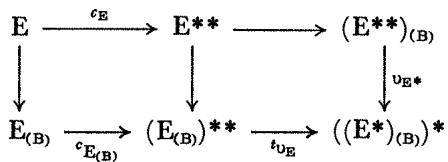
\includegraphics[keepaspectratio]{images/part003_7dd43288.jpg}}

is commutative.

\begin{enumerate}
\def\labelenumi{\arabic{enumi}.}
\setcounter{enumi}{4}
\item
  Let K be a field, A the product ring \(K^{N}\) , a the ideal \(K^{(N)}\) of A and B the ring A/a. Show that a is a projective A-module which is not finitely generated, although \(a_{(B)} = \{0\}\) .
\item
  With the rings A and B defined as in §1, Exercise 7, let M be an A-module; show that for M to be finitely generated (resp. free, projective), it is necessary and sufficient that \(M \otimes_{A} B\) be finitely generated (resp. free, projective).
\item
  Let \(\rho: A \to B\) be a ring homomorphism. For every left B-module \(F\) , define a canonical B-module homomorphism
\end{enumerate}

\[
\mathbf {F} \rightarrow \tilde {\rho} (\rho_ {*} (\mathbf {F}))
\]

and show that if E is a left A-module, the composite mappings

\[
\begin{array}{r l} & {\tilde {\rho} (\mathbf {E}) \to \tilde {\rho} (\rho_ {*} (\tilde {\rho} (\mathbf {E}))) \to \tilde {\rho} (\mathbf {E})} \\ & {\rho_ {*} (\mathbf {F}) \to \rho_ {*} (\tilde {\rho} (\rho_ {*} (\mathbf {F}))) \to \rho_ {*} (\mathbf {F})} \end{array}
\]

are the identity mappings.

\BourbakiExercisesSection

\begin{enumerate}
\def\labelenumi{\arabic{enumi}.}
\item
  Let \((\mathbf{E}_n, f_{nm})\) be the inverse system of \(\mathbf{Z}\) -modules whose indexing set is \(\mathbf{N}\) , such that \(\mathbf{E}_n = \mathbf{Z}\) for all \(n\) and, for \(n \leqslant m\) , \(f_{nm}\) is the mapping \(x \mapsto 3^{m - n}x\) . For all \(n\) , let \(u_n\) be the canonical mapping \(\mathbf{E}_n \to \mathbf{Z}/2\mathbf{Z}\) . Show that \((u_n)\) is an inverse system of surjective linear mappings but that \(\lim u_n\) is not surjective.
\item
  Let \((\mathbf{E}_{\alpha}, f_{\beta\alpha})\) be a direct system of A-modules. Show that the A-module \(\lim_{\rightarrow} E_{\alpha}\) is canonically isomorphic to the quotient of the direct sum \(\bigoplus_{\alpha} E_{\alpha} = F\) by the submodule N generated by the elements of the form \(j_{\beta}(f_{\beta\alpha}(x_{\alpha})) - j_{\alpha}(x_{\alpha})\) , for every ordered pair \((\alpha, \beta)\) such that \(\alpha \leqslant \beta\) and all \(x_{\alpha} \in E_{\alpha}\) , the \(j_{\alpha}: E_{\alpha} \to F\) being the canonical injections.
\item
  Let \((\mathbf{F}_n, f_{mn})\) be the direct system of \(\mathbf{Z}\) -modules such that \(\mathbf{F}_n\) is equal to \(\mathbf{U}_p\) ( \(\S 1\) , Exercise 12 (d)) for all \(n \geqslant 0\) and \(f_{mn}\) is the endomorphism \(x \mapsto p^{m-n}x\) of \(\mathbf{U}_p\) for \(n \leqslant m\) . Show that \(\lim_{\longrightarrow} \mathbf{F}_n = \{0\}\) although the \(f_{mn}\) are surjective.
\item
  Let \((\mathbf{F}_{\alpha}, f_{\beta \alpha})\) be a direct system of A-modules.
\end{enumerate}

\begin{enumerate}
\def\labelenumi{(\alph{enumi})}
\tightlist
\item
  For every A-module E, define a canonical Z-module homomorphism
\end{enumerate}

\[
\varepsilon : \varinjlim \operatorname{Hom} _ {\mathbf {A}} (\mathrm{E}, \mathrm{F} _ {\alpha}) \rightarrow \operatorname{Hom} _ {\mathbf {A}} (\mathrm{E}, \varinjlim \mathrm{F} _ {\alpha}).
\]

\begin{enumerate}
\def\labelenumi{(\alph{enumi})}
\setcounter{enumi}{1}
\item
  Show that if E is finitely generated, \(\varepsilon\) is injective. Give an example where \(\varepsilon\) is not injective (cf.~Exercise 3, taking \(E = \lim F_{\alpha}\) ).
\item
  Show that if E is finitely generated and the \(f_{\beta\alpha}\) are injective, \(\varepsilon\) is surjective. Give an example where \(E = \lim_{\longrightarrow} F_{\alpha}\) is free, the \(f_{\beta\alpha}\) are injective and \(\varepsilon\) is not surjective.
\item
  Show that if \(\mathbf{E}\) is projective and finitely generated, \(\varepsilon\) is bijective.
\end{enumerate}

\(^{*}(e)\) Let A be an integral domain and a an ideal of A which is not finitely generated. If \((a_{\alpha})\) is the family of finitely generated ideals contained in a, show that E = A/a is canonically isomorphic to the direct limit of the \(F_{\alpha} = A/a_{\alpha}\) , but that the homomorphism \(\varepsilon\) is not surjective.*

\BourbakiExercisesSection

\begin{enumerate}
\def\labelenumi{\arabic{enumi}.}
\item
  Show that if E is a vector space \(\neq\{0\}\) over a field K with an infinity of elements, the set of generating systems of E is not inductive for the order relation \(\supset\) (form a decreasing sequence \((S_{n})\) of generating systems of E such that the intersection of the \(S_{n}\) is empty).
\item
  Let K be a field, L a subfield of K, I a set and \((x_{i})_{1\leqslant i\leqslant m}\) a free family of vectors in \(K_{s}^{I}\) such that the coordinates of each of the \(x_{i}\) belong to L. Let V be the vector subspace of \(K_{s}^{I}\) generated by the \(x_{i}\) ; show that there exists a finite subset J of I, with m elements, such that for every vector \(z=(\zeta_{\alpha})_{\alpha\in\mathbb{I}}\) of V, all the \(\zeta_{\alpha}\) belong to the subfield of K generated by L and the m elements \(\zeta_{\beta}\) where \(\beta\in J\) . (By applying Corollary 3 of no. 5, to the space \(L_{s}^{I}\) , show that it can be reduced to the case where there exist m indices \(\beta_{i}\in I\) ( \(1\leqslant i\leqslant m\) ) such that \(\Pr_{\beta_{i}}(x_{j})=\delta_{ij}\) ).
\item
  \begin{enumerate}
  \def\labelenumii{(\alph{enumii})}
  \tightlist
  \item
    Let G be a group and M an infinite subset of G. Show that if \(G'\) is the subgroup of G generated by M, then \(\text{Card}(G') = \text{Card}(M)\) .
  \end{enumerate}
\end{enumerate}

\begin{enumerate}
\def\labelenumi{(\alph{enumi})}
\setcounter{enumi}{1}
\item
  Let \(\mathbf{K}\) be a field and \(\mathbf{M}\) an infinite subset of \(\mathbf{K}\) . Show that if \(\mathbf{K}'\) is the subfield of \(\mathbf{K}\) generated by \(\mathbf{M}\) , then \(\operatorname{Card}(\mathbf{K}') = \operatorname{Card}(\mathbf{M})\) . (Consider two sequences \((\mathbf{A}_n)_{n \geqslant 0}, (\mathbf{P}_n)_{n \geqslant 0}\) of subsets of \(\mathbf{K}\) such that \(\mathbf{A}_0 = \mathbf{M}\) , \(\mathbf{P}_n\) is the multiplicative subgroup of \(\mathbf{K}^*\) generated by \(\mathbf{A}_n \cap \mathbf{K}^*\) and \(\mathbf{A}_{n+1}\) the additive subgroup of \(\mathbf{K}\) generated by \(\mathbf{P}_n\) ; then apply (a).)
\item
  Let K be a field and I an infinite set; show that \(\operatorname{Card}(\mathbf{K}) \leqslant \dim(\mathbf{K}_{s}^{\mathbf{I}})\) . (Reduce it to the case I = N and argue by reductio ad absurdum. Let B be a basis of \(K_{s}^{N}\) such that \(\operatorname{Card}(\mathbf{B}) < \operatorname{Card}(\mathbf{K})\) and let L be the subfield of K generated by the coordinates of all the elements of B; then \(\operatorname{Card}(\mathbf{L}) < \operatorname{Card}(\mathbf{K})\) . Form a sequence \((\xi_{n})_{n \geqslant 1}\) of elements of K such that for all n, \(\xi_{n}\) does not belong to the subfield of K generated by L and the \(\xi_{i}\) of index i \textless{} n; then apply Exercise 2 to obtain a contradiction, by considering the point \(x = (\xi_{n})\) of \(K_{s}^{N}\) .
\item
  Deduce from (c) that for every field K and every infinite set I,
\end{enumerate}

\[
\dim (\mathrm{K} _ {s} ^ {\mathrm{I}}) = (\operatorname{Card} (\mathrm{K})) ^ {\operatorname{Card} (\mathrm{I})}
\]

(``Erdös-Kaplansky theorem'').

4 Give an example of an infinite sequence \((\mathbf{F}_n)\) of vector subspaces of a vector space \(\mathbf{E}\) such that \(\operatorname{codim}\left(\bigcap_{n} \mathbf{F}_n\right) > \sum_{n} \operatorname{codim}(\mathbf{F}_n)\) . (Take \(\operatorname{codim}(\mathbf{F}_n) = 1\) for all \(n\) and use Exercise 3 \((d)\) .)

\begin{enumerate}
\def\labelenumi{\arabic{enumi}.}
\setcounter{enumi}{4}
\tightlist
\item
  Let \((\mathbf{H}_{\lambda})_{\lambda \in L}\) be a family of hyperplanes (passing through 0) of a vector space \(\mathbf{E}\) over a field \(\mathbf{K}\) , which is a covering of \(\mathbf{E}\) .
\end{enumerate}

\begin{enumerate}
\def\labelenumi{(\alph{enumi})}
\item
  Show that, if K is finite, then \(\operatorname{Card}(\mathbf{L}) \geqslant 1 + \operatorname{Card}(\mathbf{K})\) and, if K is infinite, \(\operatorname{Card}(\mathbf{L}) \geqslant \aleph_{0} = \operatorname{Card}(\mathbf{N})\) . (Prove by induction on r that if K has at least r elements, then E cannot be the union of r hyperplanes.) Show by examples that these inequalities cannot be improved without an additional hypothesis (when K is infinite, consider the space \(\mathbf{E} = \mathbf{K}_{s}^{(\mathbf{N})}\) ).
\item
  If E is finite-dimensional, show that \(\operatorname{Card}(\mathbf{L}) \geqslant 1 + \operatorname{Card}(\mathbf{K})\) . (Argue by induction on \(\dim(\mathbf{E})\) .) which is no longer true in infinite dim, consider \(K^{(N)}\)
\end{enumerate}

¶ 6. Let S be a non-empty finite subset of a vector K-space E, not containing 0. Suppose that there exists an integer \(k \geqslant 1\) with the following property: (*) for all \(x \in S\) , there is a partition of \(S = \{x\}\) into \(h\) free subsets with \(h \leqslant k\) .

For such a partition \((\mathbf{N}_i)_{1\leqslant i\leqslant h}\) and every sequence \((r_j)_{1\leqslant j\leqslant m}\) of integers of \(\{1,h\}\) a subspace \(\mathrm{F}_{r_1r_2\dots r_m}\) of \(\mathbf{E}\) is defined by induction on \(m\) as follows: \(\mathrm{F}_{r_1}\) is the subspace generated by \(\mathrm{N}_{r_1},\mathrm{F}_{r_1\dots r_p}\) the subspace generated by the intersection of \(\mathrm{F}_{r_1\dots r_{p-1}}\) and \(\mathrm{N}_{r_p}\) . Suppose that:

(**) for all \(x \in S\) and every partition \((N_i)_{1 \leqslant i \leqslant h}\) of \(S = \{x\}\) into at most \(k\) free subsets, there exists at least one sequence \((r_j)_{1 \leqslant j \leqslant m}\) such that

\[
x \notin \mathrm{F} _ {r _ {1} r _ {2} \dots r _ {m}}.
\]

\begin{enumerate}
\def\labelenumi{(\alph{enumi})}
\item
  Let \(n\) be the least of the integers \(m \geqslant 1\) for all possible choices of \(x \in S\) and let \((\mathbf{N}_i)_{1 \leqslant i \leqslant h}\) and \((r_j)_{1 \leqslant j \leqslant m}\) satisfy conditions (*) and (**). Show that of necessity \(n = 1\) . (Argue by reductio ad absurdum by assuming \(x \notin F_{r_1 r_2 \ldots r_n}\) and \(n > 1\) . Then necessarily \(x \in F_{r_n}\) . For simplicity write \(E_p = F_{r_1 r_2 \ldots r_p}\) for \(1 \leqslant p \leqslant n\) and \(x = \sum_i \alpha_i y_i\) with \(\alpha_i \in K\) and \(y_i \in N_{r_n}\) ; there is at least one \(y_i\) not belonging to \(E_{n-1}\) , denote it by \(y\) ; then write \(N = N_{r_n} - \{y\}\) , \(N_i' = N_i\) for \(1 \leqslant i \leqslant h\) and \(i \neq r_n\) , \(N_{r_n}' = N \cup \{x\}\) , so that \((\mathbf{N}_i')_{1 \leqslant i \leqslant h}\) is a partition of \(S - \{y\}\) consisting of free subsets. Define \(E_0' = E\) and for \(1 \leqslant p \leqslant n\) , \(E_p'\) as the subspace generated by the intersection of \(E_{p-1}'\) and \(N_{r_p}'\) . Now \(y \notin E_{n-1}\) ; let \(q\) be the least integer such that \(y \notin E_q\) ; show that \(E_q' \not\subset E_q\) . Let \(s\) be the least integer such that \(E_s' \not\subset E_s\) ; show that \(r_s = r_n\) ; deduce finally a contradiction from the relations \(y \in E_s, E_{s-1}' \subset E_{s-1}\) and \(E_s' \not\subset E_s\) .
\item
  Conclude from (a) that with the given hypotheses there exists a partition of S into h free subsets for an integer \(h \leqslant k\) .
\end{enumerate}

\begin{enumerate}
\def\labelenumi{\arabic{enumi}.}
\setcounter{enumi}{6}
\tightlist
\item
  Let S be a non-empty finite subset of a vector K-space E, not containing 0. Suppose that there exists an integer \(k \geqslant 1\) such that for every subset
\end{enumerate}

T of S, \(\text{Card}(T) \leqslant k.\text{rg}(T)\) . Show that there exists a partition of S into h free subsets for some integer \(h \leqslant k\) . (Prove that S satisfies condition ( \(^{**}\) ) of Exercise 6, arguing by induction on \(\text{Card}(S)\) and taking amongst all the subspaces \(F_{r_{1}\ldots r_{m}}\) one of those with the smallest possible dimension; if G is such a subspace and j an index for which \(\text{Card}(G \cap N_{j})\) is the least possible, prove that

\[
\begin{array}{r l} k. \operatorname{Card} (\mathrm{G} \cap \mathrm{N} _ {j}) & \leqslant \operatorname{Card} (\mathrm{G} \cap (\mathrm{S} - \{x \})) \\ & \leqslant \operatorname{Card} (\mathrm{G} \cap \mathrm{S}) \leqslant k. \operatorname{Card} (\mathrm{G} \cap \mathrm{N} _ {j}).) \end{array}
\]

\begin{enumerate}
\def\labelenumi{\arabic{enumi}.}
\setcounter{enumi}{7}
\item
  Let E be a vector space. Show that every endomorphism of E which is not a right divisor of 0 in End(E) is surjective (§ 2, Exercise 7).
\item
  Let K be a field.
\end{enumerate}

\begin{enumerate}
\def\labelenumi{(\alph{enumi})}
\item
  In the vector space \(\mathbf{E} = \mathrm{K}_s^{(\mathbf{Z})}\) , let \((e_n)_{n\in \mathbf{Z}}\) denote the canonical basis; let \(v\) be the automorphism of \(\mathbf{E}\) defined by the relations \(v(e_n) = e_{n + 1}\) for all \(n\in \mathbf{Z}\) . If \(u = 1_{\mathbb{E}} - v\) , show that \(u\) is an injective endomorphism of \(\mathbf{E}\) , but that \(\dim (\operatorname {Coker}(u)) = 1\) .
\item
  In the vector space \(\mathbf{E} = \mathrm{K}_s^{(\mathbb{N})}\) , let \((e_n)_{n\in \mathbb{N}}\) denote the canonical basis; let \(v\) be the endomorphism of \(\mathbf{E}\) defined by \(v(e_0) = e_0\) , \(v(e_n) = e_{n - 1} + e_n\) for \(n\geqslant 1\) . Show that \(v\) is an automorphism of \(\mathbf{E}\) and that, if \(u = 1_{\mathbb{E}} - v\) , \(u\) is a surjective endomorphism of \(\mathbf{E}\) such that \(\dim (\mathrm{Ker}(u)) = 1\) .
\item
  Let I be a non-empty set. Show that every automorphism u of the vector space \(E = K_{s}^{(I)}\) can be written as a difference u = v - w of two automorphisms of E, except when K has only two elements and I consists of a single element. (Note that it suffices to prove that one particular automorphism u is of the desired form; when K is a field with two elements, consider separately the cases where \(\text{Card}(I) = 2\) and \(\text{Card}(I) = 3\) .)
\end{enumerate}

¶ 10. Let E be a vector space over a field K. Show that every endomorphism u of E is an automorphism or can be written as u = v - w, where v and w are automorphisms of E. (Observe that u can always be replaced by \(s_{1} \circ u \circ s_{2}\) , where \(s_{1}\) and \(s_{2}\) are two automorphisms of E. Distinguish two cases, according to whether \(\dim(\text{Ker}(u)) \leqslant \dim(\text{Coker}(u))\) or \(\dim(\text{Ker}(u)) > \dim(\text{Coker}(u))\) ; when \(\text{rg}(u)\) is finite, then the first case always holds. When

\[
\dim (\operatorname{Ker} (u)) \leqslant \dim (\operatorname{Coker} (u)),
\]

it can be reduced to the case where \(\operatorname{Ker}(u) \cap \operatorname{Im}(u) = \{0\}\) ; if

\[
\dim (\operatorname{Ker} (u)) = \dim (\operatorname{Coker} (u)),
\]

it can also be assumed that \(\operatorname{Im}(u) + \operatorname{Ker}(u) = \mathbf{E}\) and then apply Exercise 9 (c). If \(\dim (\operatorname {Ker}(u)) < \dim (\operatorname {Coker}(u))\) , there is a supplementary subspace in \(\mathbf{E}\) of \(\operatorname {Ker}(u)\) of the form \(\mathbf{W} \oplus \operatorname{Im}(u)\) with \(\dim (\mathbf{W}) = \dim (\operatorname {Im}(u)) = \dim (\mathbf{E})\) ; apply the remark at the beginning with \(s_1(u(\operatorname {Im}(u))) = \operatorname{Im}(u)\) and use Exercise 9 (a) and (c). When \(\dim (\operatorname {Ker}(u)) > \dim (\operatorname {Coker}(u))\) , it can be reduced to the case where \(\operatorname{Ker}(u) \subset \operatorname{Im}(u)\) ; this time take \(s_1(\operatorname{Ker}(u)) = u(\operatorname{Ker}(u))\) and use the results of the preceding cases and Exercise 9.)

\begin{enumerate}
\def\labelenumi{\arabic{enumi}.}
\setcounter{enumi}{10}
\tightlist
\item
  Let E, F be two vector spaces over a field K and \(u: E \rightarrow F\) a linear mapping. Show that for every vector subspace V of F,
\end{enumerate}

\[
\dim (u ^ {- 1} (\mathbf {V})) = \dim (\mathbf {V} \cap \operatorname{Im} (u)) + \dim (\operatorname{Ker} (u)).
\]

\begin{enumerate}
\def\labelenumi{\arabic{enumi}.}
\setcounter{enumi}{11}
\tightlist
\item
  Let E, F be two vector spaces and u, v two linear mappings of E into F.
\end{enumerate}

\begin{enumerate}
\def\labelenumi{(\alph{enumi})}
\tightlist
\item
  Show that the following inequalities hold:
\end{enumerate}

\[
\begin{array}{c} \operatorname{rg} (v) \leqslant \operatorname{rg} (u + v) + \operatorname{rg} (u) \\ \operatorname{rg} (u + v) \leqslant \inf (\dim (\mathrm{E}), \dim (\mathrm{F}), \operatorname{rg} (u) + \operatorname{rg} (v)). \end{array}
\]

If E and F are finite-dimensional, show that \(\operatorname{rg}(u + v)\) can take any integer value satisfying the inequalities

\[
\left| \operatorname{rg} (u) - \operatorname{rg} (v) \right| \leqslant \operatorname{rg} (u + v) \leqslant \inf (\dim (\mathrm{E}), \dim (\mathrm{F}), \operatorname{rg} (u) + \operatorname{rg} (v)).
\]

\begin{enumerate}
\def\labelenumi{(\alph{enumi})}
\setcounter{enumi}{1}
\tightlist
\item
  Show that
\end{enumerate}

\[
\dim (\operatorname{Ker} (u + v)) \leqslant \dim (\operatorname{Ker} (u) \cap \operatorname{Ker} (v)) + \dim (\operatorname{Im} (u) \cap \operatorname{Im} (v)).
\]

\begin{enumerate}
\def\labelenumi{(\alph{enumi})}
\setcounter{enumi}{2}
\tightlist
\item
  Show that
\end{enumerate}

\[
\dim (\operatorname{Coker} (u + v)) \leqslant \dim (\operatorname{Coker} (u)) + \operatorname{rg} (v).
\]

(If \(\mathbf{V}\) is a supplementary subspace of \(\operatorname{Ker}(v)\) in \(\mathbf{E}\) , note that

\[
u (\operatorname{Ker} (v)) \subset \operatorname{Im} (u + v) \quad \text { and } \quad \dim (u (\mathbf {V})) \leqslant \operatorname{rg} (v).)
\]

\begin{enumerate}
\def\labelenumi{\arabic{enumi}.}
\setcounter{enumi}{12}
\tightlist
\item
  Let E, F, G be three vector spaces and \(u: \mathbf{E} \to \mathbf{F}\) , \(v: \mathbf{F} \to \mathbf{G}\) two linear mappings.
\end{enumerate}

\begin{enumerate}
\def\labelenumi{(\alph{enumi})}
\tightlist
\item
  Show that there exists a decomposition of E as a direct sum of \(\operatorname{Ker}(u)\) and two subspaces M, N such that \(\operatorname{Ker}(v \circ u) = \mathbf{M} \oplus \operatorname{Ker}(u)\) and
\end{enumerate}

\[
\operatorname{Im} (v \circ u) = v (u (\mathbf {N})).
\]

\begin{enumerate}
\def\labelenumi{(\alph{enumi})}
\setcounter{enumi}{1}
\item
  \(\dim(\operatorname{Ker}(u)) \leqslant \dim(\operatorname{Ker}(v \circ u)) \leqslant \dim(\operatorname{Ker}(u)) + \dim(\operatorname{Ker}(v))\) ; if \(\operatorname{Ker}(u)\) and \(\operatorname{Ker}(v)\) are finite-dimensional, show that \(\dim(\operatorname{Ker}(v \circ u))\) can take every integer value satisfying the above inequalities.
\item
  The following equalities hold:
\end{enumerate}

\[
\begin{array}{l} \operatorname{rg} (u) = \operatorname{rg} (v \circ u) + \dim (\operatorname{Im} (u) \cap \operatorname{Ker} (v)) \\ \operatorname{rg} (v) = \operatorname{rg} (v \circ u) + \operatorname{codim} _ {\mathbb {F}} (\operatorname{Im} (u) + \operatorname{Ker} (v)). \end{array}
\]

If F is finite-dimensional, show that \(\operatorname{rg}(v \circ u)\) can take any integer value satisfying the inequality

\[
\sup (0, \operatorname{rg} (u) + \operatorname{rg} (v) - n) \leqslant \operatorname{rg} (v \circ u) \leqslant \inf (\operatorname{rg} (u), \operatorname{rg} (v)).
\]

\begin{enumerate}
\def\labelenumi{\arabic{enumi}.}
\setcounter{enumi}{13}
\item
  Let E, F, G be three vector spaces and \(u: \mathbf{E} \to \mathbf{F}\) , \(w: \mathbf{E} \to \mathbf{G}\) two linear mappings. Show that if \(u(0) \subset w(0)\) , there exists a linear mapping \(v\) of F into G such that \(w = v \circ u\) (cf.~§ 2, Exercise 8).
\item
  Let E, F be two vector spaces over a field K and \(u: E \rightarrow F\) a linear mapping.
\end{enumerate}

\begin{enumerate}
\def\labelenumi{(\alph{enumi})}
\item
  The following conditions are equivalent: (1) \(\operatorname{Ker}(u)\) is finite-dimensional; (2) there exists a linear mapping \(v\) of \(\mathbf{F}\) into \(\mathbf{E}\) such that \(v \circ u = 1_{\mathbf{E}} + w\) , where \(w\) is an endomorphism of \(\mathbf{E}\) of finite rank; (3) for every vector space \(\mathbf{G}\) over \(\mathbf{K}\) and every linear mapping \(f: \mathbf{G} \to \mathbf{E}\) , the relation \(\operatorname{rg}(u \circ f) < +\infty\) implies \(\operatorname{rg}(f) < +\infty\) .
\item
  The following conditions are equivalent: (1) Coker(u) is finite-dimensional; (2) there exists a linear mapping v of F into E such that \(u \circ v = 1_{F} + w\) , where w is an endomorphism of F of finite rank; (3) for every vector space G over K and every linear mapping \(g: F \to G\) , the relation \(\operatorname{rg}(g \circ u) < +\infty\) implies \(\operatorname{rg}(g) < +\infty\) .
\end{enumerate}

\begin{enumerate}
\def\labelenumi{\arabic{enumi}.}
\setcounter{enumi}{15}
\tightlist
\item
  Let E, F be two vector spaces over K and \(u: E \to F\) a linear mapping. u is said to be of finite index if \(\operatorname{Ker}(u)\) and \(\operatorname{Coker}(u)\) are finite-dimensional and the number \(d(u) = \dim(\operatorname{Ker}(u)) - \dim(\operatorname{Coker}(u))\) is then called the index of u.
\end{enumerate}

Let G be a third vector space over K and \(v: F \rightarrow G\) a linear mapping. Show that if two of the three linear mappings u, v, \(v \circ u\) are of finite index, so is the third and \(d(v \circ u) = d(u) + d(v)\) (use Exercise 13 (a)).

\begin{enumerate}
\def\labelenumi{\arabic{enumi}.}
\setcounter{enumi}{16}
\tightlist
\item
  Let E, F, G, H be four vector spaces over K and \(u: E \rightarrow F\) , \(v: F \rightarrow G\) , \(w: G \rightarrow H\) three linear mappings. Show that
\end{enumerate}

\[
\operatorname{rg} (v \circ u) + \operatorname{rg} (w \circ v) \leqslant \operatorname{rg} (v) + \operatorname{rg} (w \circ v \circ u).
\]

\begin{enumerate}
\def\labelenumi{\arabic{enumi}.}
\setcounter{enumi}{17}
\item
  Let E, F be two vector spaces over a field K and u, v two linear mappings of E into F. For there to exist an automorphism f of E and an automorphism g of F such that \(v = g \circ u \circ f\) , it is necessary and sufficient that \(\operatorname{rg}(u) = \operatorname{rg}(v)\) , \(\dim(\operatorname{Ker}(u)) = \dim(\operatorname{Ker}(v))\) and \(\dim(\operatorname{Coker}(u)) = \dim(\operatorname{Coker}(v))\) .
\item
  Let E be a vector space over a field K.
\end{enumerate}

\begin{enumerate}
\def\labelenumi{(\alph{enumi})}
\item
  Show that every mapping \(f\) of \(\mathbf{E}\) into \(\mathbf{E}\) which is permutable with every automorphism of \(\mathbf{E}\) is of the form \(x \mapsto \alpha x\) , where \(\alpha \in \mathbf{K}\) (show first that for all \(x \in \mathbf{E}\) there exists \(\rho(x) \in \mathbf{K}\) such that \(f(x) = \rho(x)x\) , using the fact that \(f\) commutes with every automorphism of \(\mathbf{E}\) leaving \(x\) invariant).
\item
  Let \(g\) be a mapping of \(\mathbf{E} \times \mathbf{E}\) into \(\mathbf{E}\) such that, for every automorphism \(u\) of \(\mathbf{E}\) , \(g(u(x), u(y)) = u(g(x, y))\) for all \(x, y\) in \(\mathbf{E}\) . Show that there exist two elements \(\alpha, \beta\) of \(\mathbf{K}\) such that \(g(x, y) = \alpha x + \beta y\) on the set of ordered pairs \((x, y)\) of linearly independent elements of \(\mathbf{E}\) ; moreover there exists a mapping \(\phi\) of \(\mathbf{K} \times \mathbf{K}\) into \(\mathbf{K}\) such that \(g(\lambda x, \mu x) = \phi(\lambda, \mu)x\) for all \(x \in \mathbf{E}\) (same method). If further \(g(u(x), u(y)) = u(g(x, y))\) for every endomorphism \(u\) of \(\mathbf{E}\) , then \(g(x, y) = \alpha x + \beta y\) for all \(x, y\) in \(\mathbf{E}\) . Generalize to mappings of \(\mathbf{E}^n\) into \(\mathbf{E}\) .
\end{enumerate}

\begin{enumerate}
\def\labelenumi{\arabic{enumi}.}
\setcounter{enumi}{19}
\tightlist
\item
  Let E be a vector space.
\end{enumerate}

\begin{enumerate}
\def\labelenumi{(\alph{enumi})}
\item
  Show that if M and N are two vector subspaces of E and M', N' the orthogonals of \(\mathbf{M}\) and \(\mathbf{N}\) respectively in \(\mathbf{E}^*\) , the orthogonal of \(\mathbf{M} \cap \mathbf{N}\) is \(\mathbf{M}' + \mathbf{N}'\) (cf.~§ 2, Exercise 9 (a)).
\item
  If E is infinite-dimensional, show that there exist hyperplanes \(H'\) of \(E^{*}\) such that the subspace of E orthogonal to \(H'\) reduces to 0 (consider a hyperplane containing the coordinate forms corresponding to a basis of E).
\item
  Show that if \(\mathbf{E}\) is infinite-dimensional there exists an infinite family \((\mathbf{V}_i)\) of subspaces of \(\mathbf{E}\) such that, if \(\mathbf{V}_i'\) is the subspace of \(\mathbf{E}^*\) orthogonal to \(\mathbf{V}_i\) , the subspace of \(\mathbf{E}^*\) orthogonal to \(\bigcap_{i} \mathbf{V}_i\) is distinct from \(\sum_{i} \mathbf{V}_i'\) .
\item
  Deduce from (b) that if E is infinite-dimensional, there exists a decomposition \(V' \oplus W'\) of \(E^{*}\) as a direct sum, \(W'\) being finite-dimensional, for which the sum \(V + W\) of subspaces V, W of E orthogonal respectively to \(V'\) and \(W'\) is distinct from E.
\item
  For a subspace of E to be finite-dimensional, it is necessary and sufficient that its orthogonal in \(E^{*}\) be of finite codimension.
\end{enumerate}

\begin{enumerate}
\def\labelenumi{\arabic{enumi}.}
\setcounter{enumi}{20}
\item
  With the notation of Theorem 8 of no. 6, let \(u\) denote the linear mapping \(x \mapsto (\langle x, x_i^* \rangle)\) of \(\mathbf{E}\) into \(\mathbf{K}_s^{\mathbf{I}}\) and \(y_0 = (\eta_i)\) . \(\mathbf{K}_d^{(\mathbf{I})}\) is identified with a subspace of the dual of \(\mathbf{K}_s^{\mathbf{I}}\) under the canonical mapping of \(\mathbf{K}_d^{(\mathbf{I})}\) into its bidual; then show that if \(\mathbf{N}'\) is the kernel of \(^t u\) , the condition of Theorem 3 (no. 5) expresses the fact that \(y_0\) is orthogonal to the intersection of \(\mathbf{N}'\) and \(\mathbf{K}_d^{(\mathbf{I})}\) . When \(\mathbf{I}\) is infinite and the system (21) (no. 5) is of finite rank, show that this intersection is distinct from \(\mathbf{N}'\) (note that \(\mathbf{N}'\) is then of finite codimension).
\item
  Let E and F be two vector spaces over a field K and u a linear mapping of E into F. If V is a vector subspace of E and \(V'\) the orthogonal of V in \(E^{*}\) , show that the dual of \(u(V)\) is isomorphic to \({}^{t}u(F^{*})/(V'\cap{}^{t}u(F^{*}))\) . If \(W'\) is a subspace of \(F^{*}\) such that \({}^{t}u(W')\) is finite-dimensional and W is the orthogonal of \(W'\) in F, \({}^{t}u(W')\) is isomorphic to the dual of the space \(u(E)/(W\cap u(E))\) .
\item
  Show that for a linear mapping \(u\) of a vector space \(E\) into a vector space \(F\) to be such that \(\mathrm{rg}(t u) = \mathrm{rg}(u)\) , it is necessary and sufficient that \(\mathrm{rg}(u)\) be finite (cf.~Exercise 3 (d)).
\item
  Let E be a vector space of finite dimension n \textgreater{} 1 over a commutative field K; show that, unless n = 2 and K is a field with two elements, there exists no isomorphism \(\phi\) of E onto \(E^{*}\) depending only on the vector space structure of E. (Note that if \(\phi\) is such an isomorphism, then necessarily \(\langle x, \phi(y) \rangle = \langle u(x), \phi(u(y)) \rangle\) for x, y in E and for every automorphism u of E (Set Theory, IV, § 1, no. 5).)
\item
  \begin{enumerate}
  \def\labelenumii{(\alph{enumii})}
  \tightlist
  \item
    Let K be a field and L, M two sets; there are canonical inclusions \((\mathbf{K}_{s}^{\mathbf{L}})^{(\mathbf{M})}\subset(\mathbf{K}_{s}^{(\mathbf{M})})^{\mathbf{L}}\subset\mathbf{K}_{s}^{\mathbf{L}\times\mathbf{M}}\) . Show that for two of these vector spaces to be equal, it is necessary and sufficient that one of the sets L, M be finite.
  \end{enumerate}
\end{enumerate}

\begin{enumerate}
\def\labelenumi{(\alph{enumi})}
\setcounter{enumi}{1}
\tightlist
\item
  Let \((\mathbf{E}_{\lambda})_{\lambda \in L}\) be a family of right vector spaces over \(K\) and \((\mathbf{F}_{\mu})_{\mu \in M}\) a family of left vector spaces over \(K\) . For the canonical mapping (26) (no. 7) to be bijective, it is necessary and sufficient that one of the vector spaces \(\prod_{\lambda \in L} \mathbf{E}_{\lambda}, \prod_{\mu \in M} F_{\mu}\) be finite-dimensional (use (a)).
\end{enumerate}

\begin{enumerate}
\def\labelenumi{\arabic{enumi}.}
\setcounter{enumi}{25}
\tightlist
\item
  \begin{enumerate}
  \def\labelenumii{(\alph{enumii})}
  \tightlist
  \item
    Let E, F be two left vector spaces over a field K; for the canonical homomorphism \(E^{*} \otimes_{K} F \to \operatorname{Hom}_{K}(E, F)\) to be bijective, it is necessary and sufficient that one of the spaces E, F be finite-dimensional.
  \end{enumerate}
\end{enumerate}

\begin{enumerate}
\def\labelenumi{(\alph{enumi})}
\setcounter{enumi}{1}
\tightlist
\item
  Let E be a right vector space and F a left vector space over a field K. For the canonical homomorphism \(E \otimes_{K} F \to \operatorname{Hom}_{K}(E^{*}, F)\) to be bijective, it is necessary and sufficient that E be finite-dimensional (use Exercise 3(d)).
\end{enumerate}

\begin{enumerate}
\def\labelenumi{\arabic{enumi}.}
\setcounter{enumi}{26}
\tightlist
\item
  \begin{enumerate}
  \def\labelenumii{(\alph{enumii})}
  \tightlist
  \item
    Under the hypotheses of Proposition 16 (i) (no. 7), for the canonical homomorphism (27) (no. 7) to be bijective, it is necessary and sufficient that E or F be finite-dimensional (note that the image under (27) (no. 7) of an element of \(\mathrm{Hom}_{\mathbb{K}}(\mathbf{E},\mathbf{G})\otimes_{\mathbb{L}}\mathbf{F}\) maps E to a subspace of \(\mathbf{G}\otimes_{\mathbb{L}}\mathbf{F}\) contained in a subspace of the form \(\mathbf{G}\otimes_{\mathbb{L}}\mathbf{F}'\) , where \(\mathbf{F}'\) is a finite-dimensional subspace of \(\mathbf{F}\) ).
  \end{enumerate}
\end{enumerate}

\begin{enumerate}
\def\labelenumi{(\alph{enumi})}
\setcounter{enumi}{1}
\tightlist
\item
  Under the hypotheses of Proposition 16 (ii) (no. 7), for the canonical homomorphism (28) (no. 7) to be bijective, it is necessary and sufficient that one of the ordered pairs \((\mathbf{E}_1, \mathbf{E}_2), (\mathbf{E}_1, \mathbf{F}_1), (\mathbf{E}_2, \mathbf{F}_2)\) consist of finite-dimensional vector spaces (use (a) and Exercise 7 of §4).
\end{enumerate}

\begin{enumerate}
\def\labelenumi{\arabic{enumi}.}
\setcounter{enumi}{27}
\item
  Let \(\rho: \mathbf{K} \to \mathbf{A}\) be an injective homomorphism of a field \(\mathbf{K}\) into a ring \(\mathbf{A}\) and let \(\mathbf{E}\) be a left vector space over \(\mathbf{K}\) . For the canonical mapping \((\mathbf{E}^*)_{(\mathbf{A})} \to (\mathbf{E}_{(\mathbf{A})})^*\) to be bijective, it is necessary and sufficient that \(\mathbf{E}\) be finite-dimensional or that \(\mathbf{A}\) , considered as a right vector \(\mathbf{K}\) -space, be finite-dimensional (use Exercise 25 ( \(b\) )). When one of these two cases holds, there exists a canonical bijection \((\mathbf{E}^{**})_{(\mathbf{A})} \to (\mathbf{E}_{(\mathbf{A})})^{**}\) .
\item
  Let A be an integral domain, K its field of fractions, E an A-module and T(E) its torsion module.
\end{enumerate}

\begin{enumerate}
\def\labelenumi{(\alph{enumi})}
\item
  Show that every linear form on \(\mathbf{E}\) is zero on \(\mathrm{T}(\mathrm{E})\) , so that the duals \(\mathbf{E}^*\) and \((\mathrm{E} / \mathrm{T}(\mathrm{E}))^*\) are canonically isomorphic.
\item
  Show that the canonical mapping \((\mathbf{E}^{*})_{(\mathbf{K})}\to (\mathbf{E}_{(\mathbf{K})})^{*}\) is injective and that it is bijective when \(\mathbf{E}\) is finitely generated.
\item
  Give an example of a torsion-free A-module E such that \(E^{*} = \{0\}\) and \(E_{(K)} \neq \{0\}\) .
\end{enumerate}

¶ 30. Let A be an integral domain and E, F two A-modules. Show that if x is a free element of E and y a free element of F, then \(x \otimes y \neq 0\) in \(E \otimes_{A} F\) . (Reduce it to the case where E and F are torsion-free, then to the case where E and F are finitely generated and use Exercise 29 (b) to show that there is an A-bilinear mapping f of \(E \times F\) into K such that \(f(x, y) \neq 0\) .)

*31. Let \(\mathbf{K}_0\) be a commutative field, A the polynomial ring \(\mathrm{K}_0[\mathrm{X},\mathrm{Y}]\) in two indeterminates over \(\mathbf{K}_0\) , which is an integral domain, and E the ideal \(\mathrm{AX} + \mathrm{AY}\) of A. Show that in the tensor product \(\mathbf{E} \otimes_{\mathbf{A}} \mathbf{E}\) the element \(\mathbf{X} \otimes \mathbf{Y} - \mathbf{Y} \otimes \mathbf{X}\) is \(\neq 0\) and that \(\mathrm{XY}(\mathbf{X} \otimes \mathbf{Y} - \mathbf{Y} \otimes \mathbf{X}) = 0\) (consider the A-bilinear mappings of \(\mathbf{E} \times \mathbf{E}\) into the quotient module \(\mathbf{A}/\mathbf{E}\) ).*

\begin{enumerate}
\def\labelenumi{\arabic{enumi}.}
\setcounter{enumi}{31}
\item
  Extend the results of no. 10 to the case where A is a non-commutative ring admitting a field of left fractions K (I, §9, Exercise 15). (Note that if \(\xi_{i}\) ( \(1 \leqslant i \leqslant n\) ) are elements of K, there exists an \(\alpha \neq 0\) in A such that all the \(\alpha\xi_{i}\) belong to A.)
\item
  Let A be an integral domain. An A-module E is called divisible if for all \(x \in E\) and all \(\alpha \neq 0\) in A, there exists \(y \in E\) such that \(\alpha y = x\) .
\end{enumerate}

\begin{enumerate}
\def\labelenumi{(\alph{enumi})}
\item
  Let E, F be two A-modules. Show that if E is divisible, so is \(E \otimes_{A} F\) . If E is divisible and F is torsion-free, \(\operatorname{Hom}_{\mathbf{A}}(\mathbf{E}, \mathbf{F})\) is torsion-free. If E is a torsion A-module and F is divisible, then \(E \otimes_{A} F = \{0\}\) . If E is a torsion A-module and F is torsion-free, then \(\operatorname{Hom}_{\mathbf{A}}(\mathbf{E}, \mathbf{F}) = \{0\}\) .
\item
  Show that every injective A-module (§ 2, Exercise 11) is divisible and conversely that every divisible torsion-free A-module is injective (use criterion (δ) of 2, Exercise 11).
\end{enumerate}

\begin{enumerate}
\def\labelenumi{\arabic{enumi}.}
\setcounter{enumi}{33}
\tightlist
\item
  Let A be an integral domain, P a projective A-module, \(P'\) a projective submodule of P and \(j: P' \to P\) the canonical injection. Show that for every torsion-free A-module E, the homomorphism \(j \otimes 1: P' \otimes_{A} E \to P \otimes_{A} E\) is injective (reduce it to the case where E is finitely generated and embed E in a free A-module).
\end{enumerate}

¶ 35. (a) Let K be a field and E a (K, K)-bimodule. Suppose that the dimensions of E, as a left and right vector space over K, are equal to the same finite number n.~Show that there exists a family \((e_{i})\) of n elements of E, which is a basis for each of the two vector space structures on E. (Note that if \((b_{j})_{1\leq j\leq m}\) is a family of m\textless n elements of E, which is free for each of the two vector space structures on E and V is the left vector subspace and W the right vector subspace generated by \((b_{j})\) , either \(V+W\neq E\) , or \(V\cap CW\) and \(W\cap CV\) are non-empty; in the latter case, if \(y\in V\cap CW\) , \(z\in W\cap CV\) , \(y+z\) forms with the \(b_{j}\) a family of \(m+1\) elements which is free for each of the two vector space structures on E.)

\begin{enumerate}
\def\labelenumi{(\alph{enumi})}
\setcounter{enumi}{1}
\item
  Let F be a subbimodule of E, whose two vector space structures over K have the same dimension p \textless{} n.~Show that there exists a family \((e_{i})_{1 \leqslant i \leqslant n}\) of elements of E which is a basis of E for each of its vector space structures and such that \((e_{i})_{1 \leqslant i \leqslant p}\) is a basis of F for each of its two vector space structures (same method).
\item
  Let \((b_{j})_{1\leqslant j\leqslant n - 1}\) be a family of \(n - 1\) elements of \(\mathbf{E}\) , which is free for each of the two vector space structures on \(\mathbf{E}\) . Let \(\mathbf{V}\) (resp. W) be the hyperplane generated by the \((b_{j})\) in \(\mathbf{E}\) considered as a left (resp. right) vector space.
\end{enumerate}

Show that if \(\mathbf{V} \subset \mathbf{W}\) (resp. \(\mathbf{W} \subset \mathbf{V}\) ), then necessarily \(\mathbf{V} = \mathbf{W}\) (note that if \(a \notin \mathbf{W}\) , the set of \(\lambda \in \mathbf{K}\) such that \(\lambda a \in \mathbf{W}\) is a left ideal).

*36. (a) Let \(\mathbf{K}_0\) be a commutative field and \(\mathbf{K} = \mathbf{K}_0(\mathbf{X})\) the field of rational functions in one indeterminate over \(\mathbf{K}_0\) (Chapter IV). A (K, K)-bimodule structure is defined on K as follows: the product \(t.u\) of an element \(u \in \mathbf{K}\) by a left operator \(t \in \mathbf{K}\) is the rational function \(t(\mathbf{X})u(\mathbf{X})\) ; the product \(u.t\) of \(u\) by a right operator \(t \in \mathbf{K}\) is the rational function \(u(\mathbf{X})t(\mathbf{X}^2)\) ; the left (resp. right) vector K-space structure thus defined on K is then 1-dimensional (resp. 2-dimensional). Deduce examples of (K, K)-bimodules such that dimensions of the two vector space structures of such a bimodule are arbitrary integers.

\begin{enumerate}
\def\labelenumi{(\alph{enumi})}
\setcounter{enumi}{1}
\tightlist
\item
  Deduce from (a) an example of a (K, K)-bimodule E whose two vector space structures have the same dimension and such that there exists a sub-bimodule F of E whose two vector space structures do not have the same dimension.*
\end{enumerate}

¶ 37. (a) Let E be a left vector space (finite-dimensional or otherwise) and \(A_{i}\) ( \(1 \leqslant i \leqslant n\) ) vector subspaces of E. Suppose that, for every sequence \((a_{i})_{1 \leqslant i \leqslant n}\) of points of E such that \(a_{i} \in A_{i}\) for all i, the vector subspace of E generated by the \(a_{i}\) is of dimension \(\leqslant m\) (m an integer \(\leqslant n\) ). Then prove that there exists a subspace W of E of dimension \(h \leqslant m\) , containing \(h + (n - m)\) of the subspaces \(A_{i}\) . (Argue by induction on n.~Prove first that (for fixed n) attention may be confined to the case where m \textless{} n and \(\dim(A_{i}) \leqslant m\) for all i; it may also be assumed that \(A_{i} \neq \{0\}\) for all i and that the \(A_{i}\) are not all

of dimension 1. Then argue (for fixed \(n\) ) by induction on \(d = \sum_{i=1}^{m} \dim(A_i)\) . If for example \(\dim(A_n) \geqslant 2\) , consider a 1-dimensional subspace \(B_n\) of \(A_n\) of dimension 1 and apply the induction hypothesis to \(A_1, \ldots, A_{n-1}, B_n\) ; conclude that there exists a number \(k\) such that \(1 \leqslant k \leqslant m\) and a \(k\) -dimensional subspace U of E containing \(k\) of the \(A_i\) , for example \(A_1, \ldots, A_k\) ; replacing, if need be, \(k\) by an integer \(k'\) such that \(1 \leqslant k' \leqslant k\) , show also that it can be assumed that there exist vectors \(b_i \in A_i\) for \(1 \leqslant i \leqslant k\) such that \(b_1, \ldots, b_k\) form a basis of U; then project onto a supplementary subspace of U in E and use the induction hypothesis.)

\begin{enumerate}
\def\labelenumi{(\alph{enumi})}
\setcounter{enumi}{1}
\tightlist
\item
  Let K be a finite field and let E be an N-dimensional vector space over K. Let \(U_{i}\) ( \(1 \leqslant i \leqslant n\) ) be vector subspaces of E such that, for every subset H of \([1, n]\) , the intersection of the \(U_{i}\) such that \(i \in H\) has dimension \(\leqslant N - \text{Card}(H)\) . Show that the union of the \(U_{i}\) cannot be equal to E (argue by duality using (a)).
\end{enumerate}

\begin{enumerate}
\def\labelenumi{\arabic{enumi}.}
\setcounter{enumi}{37}
\item
  Let K be a commutative field of characteristic 0 and E a finite-dimensional vector space over K. Let \(p_{1}, \ldots, p_{m}\) be projectors of E onto vector subspaces of E such that \(1_{E} = p_{1} + p_{2} + \cdots + p_{m}\) . Show that E is the direct sum of the \(p_i(\mathbf{E})\) and that the \(p_i\) are pairwise permutable (take the traces of the two sides).
\item
  Let K be a field, L a subfield of K and \((\mathrm{K}_{\alpha})_{\alpha\in I}\) a left directed family of subfields of K such that \(L=\bigcap_{\alpha\in I}K_{\alpha}\) . Let E be a vector space over K and \((a_{i})_{1\leqslant i\leqslant m}\) a finite family of elements of E; show that if the family \((a_{i})\) is free over L, there exists an index \(\alpha\) such that \((a_{i})\) is free over \(K_{\alpha}\) . (Argue by induction on m-r, where r is the rank of the family \((a_{i})\) over K.)
\end{enumerate}

\BourbakiExercisesSection

\begin{enumerate}
\def\labelenumi{\arabic{enumi}.}
\tightlist
\item
  Let K be a field, \(K'\) a subfield of K and V a non-zero right vector space over K.
\end{enumerate}

\begin{enumerate}
\def\labelenumi{(\alph{enumi})}
\item
  Let \(\mathbf{V}'\) be a \(\mathbf{K}'\) -structure on \(\mathbf{V}\) . Show that \(\mathbf{K}'\) is equal to the set of \(\mu \in \mathbf{K}\) such that, for all \(x \in \mathbf{V}'\) , \(x\mu \in \mathbf{V}'\) .
\item
  Let \(\Gamma'\) be the group of automorphisms of K leaving invariant the elements of K'. Show that if there exists no element of K not belonging to K' and invariant under all the automorphisms \(\sigma \in \Gamma'\) , there exists no element of V not belonging to V' and invariant under every bijective dimorphism of V (relative to an automorphism of K) which leaves invariant all the elements of V'.
\item
  Conversely, let E be a subset of V and G the group of bijective dimorphisms of V leaving invariant all the elements of E; for all \(u \in G\) , let \(\sigma_{u}\) be the corresponding automorphism of K and let \(\Gamma\) be the group of automorphisms of K the image of G under the homomorphism \(u \mapsto \sigma_{u}\) . Suppose that G contains no automorphism of V distinct from the identity automorphism and that there exists no element of V not belonging to E and invariant under all the dimorphisms \(u \in G\) . Show that if \(K'\) is the subfield of elements of K invariant under all the automorphism \(\sigma \in \Gamma\) , E is a \(K'\) -structure on V. (Prove first that E is an additive subgroup of V containing a basis of V; let \(K''\) be the set of elements \(\mu \in K\) such that the relation \(x \in E\) implies \(x\mu \in E\) . Show that the elements of \(K''\) are invariant under all \(\sigma \in \Gamma\) and that \(K''\) is a subfield of K; deduce that E is a \(K''\) -structure on V.)
\end{enumerate}

\begin{enumerate}
\def\labelenumi{\arabic{enumi}.}
\setcounter{enumi}{1}
\tightlist
\item
  Let K be a field, \(K'\) a subfield of K, V a right vector space over K, \(V'\) a \(K'\) -structure on V and \(R'\) the canonical image of the dual \(V'*\) in the dual \(V*\) of V (no. 4). For \(R'\) to be a generating system of \(V*\) , it is necessary and sufficient that V be finite-dimensional or that K be a finite-dimensional right vector \(K'\) -space (use Exercise 25 of §7).
\end{enumerate}

¶ 3. Let K be a field, L a subfield of K and let \(K_{L}\) denote the field K considered as a left vector space over L; \(E = \text{End}_{L}(K_{L})\) has canonically a (K, K)-bimodule structure. The dual \((K_{L})^{*}\) is contained in E and is a (K, L)-sub-bimodule of E. When L is contained in the centre of K, the two vector L-space structures on E, obtained by restricting to L the field of scalars of the two vector K-space structures on E, are identical.

Suppose henceforth that \(\mathbf{L}\) is contained in the centre of \(\mathbf{K}\) and that the dimension of \(\mathbf{K}_{\mathbf{L}}\) is finite and equal to \(n\) .

\begin{enumerate}
\def\labelenumi{(\alph{enumi})}
\item
  Show that \((\mathrm{K}_{\mathrm{L}})^{*}\) is 1-dimensional under its left vector space structure over K (calculate the dimension of \((\mathrm{K}_{\mathrm{L}})^{*}\) over L in two ways).
\item
  Show that \(\mathbf{E}\) is an \(n\) -dimensional left vector space over \(\mathbf{K}\) (same method).
\item
  Let F be a finite-dimensional left vector space over K and \(F_{[L]}\) the corresponding vector space over L. If \(u_{0} \neq 0\) is a linear form on \(K_{L}\) , show that the mapping \(x' \mapsto u_{0} \circ x'\) of the dual \(F^{*}\) of F (considered as a vector space over L) onto the dual \((\mathrm{F}_{[\mathrm{L}]})^{*}\) of \(F_{[L]}\) is bijective (use (a)).
\end{enumerate}

¶ 4. Let K be a field of finite rank over its centre Z and L a subfield of K containing Z.

\begin{enumerate}
\def\labelenumi{(\alph{enumi})}
\item
  Show that the left and right vector space structures of K with respect to L have the same dimension.
\item
  Show that properties (a), (b), (c) of Exercise 3 also hold in this case (if \(u_0\) is a linear form \(\neq 0\) on \(\mathbf{L}_{\mathbf{Z}}\) and \(v_0\) a linear form \(\neq 0\) on \(\mathbf{K}_{\mathbf{L}}\) , note that \(\xi. (u_0 \circ v_0) = u_0 \circ (\xi v_0)\) for \(\xi \in \mathbf{K}\) , that \(\xi. (u_0 \circ v_0)\) runs through the dual \((\mathbf{K}_{\mathbf{Z}})^*\) when \(\xi\) runs through \(\mathbf{K}\) and use Exercise 3 (c)).
\end{enumerate}

\begin{enumerate}
\def\labelenumi{\arabic{enumi}.}
\setcounter{enumi}{4}
\tightlist
\item
  Let \(K_{0}\) be a subfield of a field K such that K is of dimension 2 as a right vector space over \(K_{0}\) . Let E be a left vector space over K.
\end{enumerate}

\begin{enumerate}
\def\labelenumi{(\alph{enumi})}
\item
  Let \(E_{0}\) be a subset of E which is a vector space over \(K_{0}\) and let V be the largest vector sub-K-space of \(E_{0}\) ; if \(W_{0}\) is a vector sub- \(K_{0}\) -space of \(E_{0}\) supplementary to V, show that the vector sub-K-space W of E generated by \(W_{0}\) is such that \(V \cap W = \{0\}\) (note that if an element \(\mu \in K\) does not belong to \(K_{0}\) , the relation \(\mu x \in E_{0}\) for an \(x \in E_{0}\) implies \(x \in V\) ).
\item
  Let \(E_{0}^{\prime}\) be another vector sub- \(K_{0}\) -space of E and \(V^{\prime}\) the largest vector sub-K-space of \(E_{0}^{\prime}\) . For there to exist a K-automorphism of E mapping \(E_{0}\) to \(E_{0}^{\prime}\) , it is necessary and sufficient that V and \(V^{\prime}\) have the same dimension with respect to K, that the codimensions of V in \(E_{0}\) and \(V^{\prime}\) in \(E_{0}^{\prime}\) (with respect to \(K_{0}\) ) be equal and that the codimensions of \(E_{0}\) and \(E_{0}^{\prime}\) in E (with respect to \(K_{0}\) ) be equal (use (a)).
\end{enumerate}

\BourbakiExercisesSection

*1. In an affine space \(\mathbf{E}\) over a field \(\mathbf{K}\) , a quadruple \((a, b, c, d)\) of points of \(\mathbf{E}\) is called a parallelogram if \(b - a = c - d\) , in which case \((a, d, c, b)\) is also a parallelogram. Show that if \(\mathbf{K}\) is of characteristic \(\neq 2\) the midpoints of the ordered pairs \((a, c)\) and \((b, d)\) are then equal; what can be said when \(\mathbf{K}\) is of characteristic \(2?_{*}\) .

*2. Let E be an affine space over a field of characteristic \(\neq 2\) and \(a, b, c, d\) any four points of E. Show that if \(x, y, z, t\) are the respective midpoints of the ordered pairs \((a, b), (b, c), (c, d), (d, a)\) , the quadruple \((x, y, z, t)\) is a parallelogram (Exercise 1).*

*3. Let K be a commutative field of characteristic \(\neq 2\) , E an affine plane over K and \(a, b, c, d\) four points of E any three of which do not lie on a straight line. Let \(\mathbf{D}_{xy}\) denote the line passing through two distinct points \(x, y\) of E. Suppose that the lines \(\mathbf{D}_{ab}\) and \(\mathbf{D}_{cd}\) have a common point \(e\) and that \(\mathbf{D}_{ad}\) and \(\mathbf{D}_{bc}\) have a common point \(f\) . Show that the midpoints of the three ordered pairs \((a, c), (b, d), (e, f)\) lie on a straight line. What becomes of this property when \(\mathbf{D}_{ab}\) and \(\mathbf{D}_{cd}\) are parallel or when \(\mathbf{D}_{ad}\) and \(\mathbf{D}_{bc}\) are parallel? Consider the case where K is a field with 3 elements.*

*4. Let K be a field whose characteristic is different from 2 and 3, E an affine space over K, \(a, b, c\) three points of E not on a straight line and \(a', b', c'\) the respective midpoints of the ordered pairs \((b, c)\) , \((c, a)\) and \((a, b)\) . Show that (in the notation of Exercise 3) the lines \(\mathbf{D}_{aa'}\) , \(\mathbf{D}_{bb'}\) and \(\mathbf{D}_{cc'}\) pass through the barycentre of the three points \(a, b, c\) . What becomes of this property when K is of characteristic 2 or of characteristic 3? Generalize to a system of \(n\) affinely independent points.*

\begin{enumerate}
\def\labelenumi{\arabic{enumi}.}
\setcounter{enumi}{4}
\item
  For a non-empty subset V of an affine space E over a field K with at least three elements to be a linear variety, it is necessary and sufficient that for every ordered pair \((x,y)\) of distinct points of V the line \(D_{xy}\) passing through x and y be entirely contained in V. If K has two elements, for V to be a linear variety, it is necessary and sufficient that the barycentre of any three points of V belong to V.
\item
  \begin{enumerate}
  \def\labelenumii{(\alph{enumii})}
  \tightlist
  \item
    Let E be an affine space of dimension \(\geqslant2\) over a field K. For an affine mapping u of E into itself to transform every line of E into a parallel line, it is necessary and sufficient that the linear mapping v associated with u be a homothety \(t\mapsto\gamma t\) of ratio \(\gamma\neq0\) belonging to the centre of K. If \(\gamma=1\) , u is a translation; show that if \(\gamma\neq1\) , there exists one and only one point \(a\in E\) such that \(u(a)=a\) . If a is taken as origin of E, u is then identified with a central homothety for the vector space structure thus determined on E; u is called a central homothety of the affine space E of centre a and ratio \(\gamma\) .
  \end{enumerate}
\end{enumerate}

\begin{enumerate}
\def\labelenumi{(\alph{enumi})}
\setcounter{enumi}{1}
\item
  Let \(u_1, u_2\) be two affine mappings of \(\mathbf{E}\) into \(\mathbf{E}\) each of which is either a translation or a central homothety. Show that \(u_1 \circ u_2\) is a translation or a central homothety of \(\mathbf{E}\) ; if \(u_1, u_2\) and \(u_1 \circ u_2\) are all three central homotheties show that their centres lie on a straight line. What can be said when \(u_1\) and \(u_2\) are central homotheties and \(u_1 \circ u_2\) is a translation?
\item
  Show that the set of translations and central homotheties is a normal subgroup H of the affine group of E and that H/T is isomorphic to the multiplicative group of the centre of K: show that H can only be commutative if H = T, in other words if the centre of K has only two elements.
\end{enumerate}

¶ 7. Let E (resp. E') be an affine space of finite dimension \(n \geqslant 2\) over field K with at least 3 elements (resp. over a field K') and let u be an injective mapping of E into E' mapping any three points in a straight line in E to three points in a straight line and such that the affine linear variety generated by \(u(E)\) in E' is equal to E'.

\begin{enumerate}
\def\labelenumi{(\alph{enumi})}
\item
  Show that \(u\) maps every system of affinely independent points of \(E\) to a system of affinely independent points (use Exercise 5).
\item
  Let \(D_{1}, D_{2}\) be two parallel lines in E and \(D_{1}^{\prime}, D_{2}^{\prime}\) the lines of \(E^{\prime}\) containing respectively \(u(\mathbf{D}_{1})\) and \(u(\mathbf{D}_{2})\) . Show that \(D_{1}^{\prime}\) and \(D_{2}^{\prime}\) are in the same plane; if further u is surjective, show that \(D_{1}^{\prime}\) and \(D_{2}^{\prime}\) are parallel (in the contrary case, show that there would be 3 points not in a straight line in E whose images under u would be in a straight line) (cf.~Exercise 17).
\item
  Suppose henceforth that if \(D_{1}\) and \(D_{2}\) are parallel lines in E, the lines of \(E'\) containing respectively \(u(\mathbf{D}_{1})\) and \(u(\mathbf{D}_{2})\) are parallel. Show that if an origin a in E and the origin \(a' = u(a)\) in \(E'\) are taken, there exists an isomorphism \(\sigma\) of K onto a subfield \(K_{1}\) of \(K'\) such that if E is considered as a vector space over K and \(E'\) as a vector space over \(K_{1}, u\) is an injective semi-linear mapping (relative to \(\sigma\) ) of E into \(E'\) (§ 1, no. 13). (Consider first the case n = 2; given a basis \((e_{1}, e_{2})\) of E, show that for any two elements \(\alpha, \beta\) of K, the points \((\alpha + \beta)e_{1}\) and \((\alpha\beta)e_{1}\) of E can be constructed starting with the points 0, \(e_{1}, e_{2}, \alpha e_{1}, \beta e_{1}\) by constructing parallels to given lines and intersections of given lines; deduce that \(u(\lambda e_{1}) = \lambda^{\sigma}u(e_{1})\) , where \(\sigma\) is an isomorphism of K onto a subfield of \(K'\) , then show that also \(u(\lambda e_{2}) = \lambda^{\sigma}u(e_{2})\) by considering the line joining the points \(\lambda e_{1}\) and \(\lambda e_{2}\) . Pass finally from here to the case where n is arbitrary, arguing by induction on n.) If u is bijective, show that \(K_{1} = K'\) .
\item
  Extend the result of (c) to the case where K is a field with 2 elements assuming also that u maps every system of affinely independent points of E to a system of affinely independent points of E'.
\end{enumerate}

\begin{enumerate}
\def\labelenumi{\arabic{enumi}.}
\setcounter{enumi}{7}
\tightlist
\item
  Let E be a left affine space over a field K and T its translation space.
\end{enumerate}

\begin{enumerate}
\def\labelenumi{(\alph{enumi})}
\tightlist
\item
  For a mapping \(f\) of \(\mathbf{E}\) into a left vector space \(\mathbf{L}\) over \(\mathbf{K}\) to be affine, it is necessary and sufficient that
\end{enumerate}

\[
\begin{array}{r l} f (\mathbf {t} + x) - f (x) & = f (\mathbf {t} + y) - f (y) \\ f (\lambda \mathbf {t} + x) - f (x) & = \lambda f (\mathbf {t} + x) - f (x)) \end{array}
\]

for all \(\lambda\in\mathbf{K},\mathbf{t}\in\mathbf{T},x,y\) in E. Let \(x\mapsto[x]\) be the canonical injection of E into the vector space \(\mathrm{K}_{s}^{(\mathbb{E})}\) of formal linear combinations of elements of E and let N be the subspace of \(\mathrm{K}_{s}^{(\mathbb{E})}\) generated by the elements

\[
[ \mathbf {t} + x ] - [ x ] - [ \mathbf {t} + y ] + [ y ]
\]

\[
[ \lambda \mathbf {t} + x ] - [ x ] - \lambda [ \mathbf {t} + x ] + \lambda [ x ]
\]

for \(\lambda \in \mathbf{K}\) , \(\mathbf{t} \in \mathbf{T}\) , \(x, y\) in \(\mathbf{E}\) ; finally, let \(\mathbf{V}\) be the quotient space of \(\mathbf{K}_s^{(\mathbf{E})}\) by \(\mathbf{N}\) and \(\phi\) the mapping of \(\mathbf{E}\) into \(\mathbf{V}\) which associates with every \(x \in \mathbf{E}\) the class of \([x]\) modulo \(\mathbf{N}\) . Then \(\phi\) is an affine mapping and for every affine mapping \(f\) of \(\mathbf{E}\) into a left vector space \(\mathbf{L}\) over \(\mathbf{K}\) , there exists one and only one linear mapping \(g\) of \(\mathbf{V}\) into \(\mathbf{L}\) such that \(f = g \circ \phi\) .

\begin{enumerate}
\def\labelenumi{(\alph{enumi})}
\setcounter{enumi}{1}
\tightlist
\item
  Let \(\phi_0: \mathbf{T} \to \mathbf{V}\) be the linear mapping associated with \(\phi\) , so that \(\phi(\mathbf{t} + x) - \phi(x) = \phi_0(\mathbf{t})\) . Show that \(\phi\) (and therefore also \(\phi_0\) ) is injective (consider the mapping \(x \mapsto x - a\) of \(\mathbf{E}\) into \(\mathbf{T}\) for some \(a \in \mathbf{E}\) ); for every family \((\lambda_t)_{t \in I}\) of elements of \(\mathbf{K}\) with finite support and every family \((x_t)_{t \in I}\) of elements of \(\mathbf{E}\) ,
\end{enumerate}

\[
\sum_ {i} \lambda_ {i} \phi (x _ {i}) = \phi_ {0} \left(\sum_ {i} \lambda_ {i} x _ {i}\right) \quad \text { if } \quad \sum_ {i} \lambda_ {i} = 0
\]

\[
\sum_ {i} \lambda_ {i} \phi (x _ {i}) = \mu \phi_ {0} \left(\sum_ {i} \mu^ {- 1} \lambda_ {i} x _ {i}\right) \quad \text { if } \quad \sum_ {i} \lambda_ {i} = \mu \neq 0.
\]

Deduce that \(\phi_{0}(T)\) is a hyperplane passing through 0 in V and \(\phi(E)\) a hyperplane parallel to \(\phi_{0}(T)\) .

\begin{enumerate}
\def\labelenumi{\arabic{enumi}.}
\setcounter{enumi}{8}
\tightlist
\item
  Let \(\mathbf{K}\) be a finite field with \(q\) elements and \(\mathbf{V}\) an \(n\) -dimensional vector space over \(\mathbf{K}\) .
\end{enumerate}

\begin{enumerate}
\def\labelenumi{(\alph{enumi})}
\tightlist
\item
  Show that the set of sequences \((x_{1}, x_{2}, \ldots, x_{m})\) of \(m \leqslant n\) vectors of \(\mathbf{V}\) forming a free system has cardinal equal to
\end{enumerate}

\[
(q ^ {n} - 1) (q ^ {n} - q) \dots (q ^ {n} - q ^ {m - 1})
\]

(argue by induction on \(n\) ).

\begin{enumerate}
\def\labelenumi{(\alph{enumi})}
\setcounter{enumi}{1}
\tightlist
\item
  Deduce from (a) that the cardinal of the set of \(m\) -dimensional linear varieties in an \(n\) -dimensional projective space over \(K\) is equal to
\end{enumerate}

\[
\frac {(q ^ {n + 1} - 1) (q ^ {n + 1} - q) \dots (q ^ {n + 1} - q ^ {m})}{(q ^ {m + 1} - 1) (q ^ {m + 1} - q) \dots (q ^ {m + 1} - q ^ {m})}.
\]

\begin{enumerate}
\def\labelenumi{\arabic{enumi}.}
\setcounter{enumi}{9}
\item
  In an \(n\) -dimensional projective space \(\mathbf{P}(\mathbf{V})\) over a field \(\mathbf{K}\) , a projective basis is a set \(\mathbf{S}\) of \(n + 2\) points any two of which form a projectively free system. If \(\mathbf{S} = (a_i)_{0 \leqslant i \leqslant n + 1}\) and \(\mathbf{S}' = (a_i')_{0 \leqslant i \leqslant n + 1}\) are any two projective bases of \(\mathbf{P}(\mathbf{V})\) , show that there exists a transformation \(f \in \mathbf{PGL}(\mathbf{V})\) such that \(f(a_i) = a_i'\) for \(0 \leqslant i \leqslant n + 1\) . For this transformation to be unique, it is necessary and sufficient that \(\mathbf{K}\) be commutative. (Reduce it to the case where \(a_i' = a_i\) for all \(i\) and note that it is always possible to write (in the notation of no. 6) \(a_i = \pi(b_i)\) , where \((b_i)_{1 \leqslant i \leqslant n + 1}\) is a basis of \(\mathbf{V}\) and \(b_0 = b_1 + b_2 + \cdots + b_{n+1}\) .) *Give an example where \(\mathbf{K}\) is a field of quaternions and there exists an infinite set \(\mathbf{T}\) of points of \(\mathbf{P}(\mathbf{V})\) any \(n + 1\) of which form a projectively free system and a transformation \(f \in \mathbf{PGL}(\mathbf{V})\) , distinct from the identity, leaving invariant all the points of \(\mathbf{T}\) .*
\item
  Let V be a 2-dimensional vector space over a field K and a, b, c, d four distinct points of the projective line \(\mathbf{P}(\mathbf{V})\) . The cross-ratio of the quadruple \((a, b, c, d)\) , denoted by \(\begin{bmatrix} a & b \\ d & c \end{bmatrix}\) , is the set of elements \(\xi \in \mathbf{K}\) such that there exist two vectors \(u, v\) in \(\mathbf{V}\) for which (in the notation of no. 6) \(a = \pi(u)\) , \(b = \pi(v)\) , \(c = \pi(u + v)\) , \(d = \pi(u + \xi v)\) . This definition extends immediately to any quadruple of distinct points of a set with a projective line structure (no. 11).
\end{enumerate}

\begin{enumerate}
\def\labelenumi{(\alph{enumi})}
\item
  Show that \(\begin{bmatrix} a & b \\ d & c \end{bmatrix}\) is the set of conjugates of an element \(\neq 1\) of the multiplicative group \(\mathbf{K}^*\) and conversely that, when \(a, b, c\) , are distinct points of \(\mathbf{P}(V)\) and \(\rho\) the set of conjugates of an element \(\neq 1\) of \(\mathbf{K}^*\) , there exists a point \(d \in \mathbf{P}(V)\) such that \(\begin{bmatrix} a & b \\ d & c \end{bmatrix} = \rho\) . For \(d\) to be unique, it is necessary and sufficient that \(\rho\) consist of a single point.
\item
  Show that
\end{enumerate}

\[
\left[ \begin{array}{c c} a & b \\ c & d \end{array} \right] = \left[ \begin{array}{c c} b & a \\ d & c \end{array} \right] = \left[ \begin{array}{c c} a & b \\ d & c \end{array} \right] ^ {- 1}
\]

and

\[
\left[ \begin{array}{c c} d & a \\ c & b \end{array} \right] = 1 - \left[ \begin{array}{c c} a & b \\ d & c \end{array} \right]
\]

(denoting by \(\rho^{-1}\) (resp. \(1 - \rho\) ) the set of conjugates \(\lambda \xi^{-1} \lambda^{-1} = (\lambda \xi \lambda^{-1})^{-1}\) (resp. \(1 - \lambda \xi \lambda^{-1} = \lambda (1 - \xi) \lambda^{-1}\) ), where \(\xi\) is an element of \(\rho\) ).

\begin{enumerate}
\def\labelenumi{(\alph{enumi})}
\setcounter{enumi}{2}
\tightlist
\item
  Let \((a, b, c, d)\) , \((a', b', c', d')\) be two quadruples of distinct points of \(\mathbf{P}(\mathbf{V})\) . For there to exist a bijective semi-linear mapping of V onto itself such that the bijective mapping f of \(\mathbf{P}(\mathbf{V})\) onto itself, obtained when passing to the quotients, satisfies the conditions \(f(a) = a'\) , \(f(b) = b'\) , \(f(c) = c'\) , \(f(d) = d'\) , it is necessary and sufficient that there exist an automorphism \(\sigma\) of K such that
\end{enumerate}

\[
\left[ \begin{array}{c c} a ^ {\prime} & b ^ {\prime} \\ d ^ {\prime} & c ^ {\prime} \end{array} \right] = \left[ \begin{array}{c c} a & b \\ d & c \end{array} \right] ^ {\sigma}.
\]

For there to exist a transformation f of the projective group PGL(V) satisfying the above conditions, it is necessary and sufficient that

\[
\left[ \begin{array}{c c} a ^ {\prime} & b ^ {\prime} \\ d ^ {\prime} & c ^ {\prime} \end{array} \right] = \left[ \begin{array}{c c} a & b \\ d & c \end{array} \right].
\]

\begin{enumerate}
\def\labelenumi{\arabic{enumi}.}
\setcounter{enumi}{11}
\tightlist
\item
  Let \(\mathbf{P}(\mathbf{V})\) be a (left) projective space of finite dimension \(n\) over a field \(\mathbf{K}\) . Show that there exists on the set of projective hyperplanes of \(\mathbf{P}(\mathbf{V})\) an \(n\) -dimensional (right) projective space structure over \(\mathbf{K}\) canonically isomorphic to that of \(\mathbf{P}(\mathbf{V}^*)\) ( \(\mathbf{V}^*\) being the dual of \(\mathbf{V}\) ). If \(\mathbf{M}\) is a linear variety of dimension \(r < n\) in \(\mathbf{P}(\mathbf{V})\) , derive an \((n - r - 1)\) -dimensional projective space structure on the set of projective hyperplanes containing \(\mathbf{M}\) . In particular if \(\mathbf{M}\) is of dimension \(n - 2\) , the cross-ratio \(\begin{bmatrix} \mathrm{H}_1 & \mathrm{H}_2 \\ \mathrm{H}_4 & \mathrm{H}_3 \end{bmatrix}\) of a quadruple \((\mathrm{H}_1, \mathrm{H}_2, \mathrm{H}_3, \mathrm{H}_4)\) of distinct hyperplanes containing M can be defined. Show that if \(\mathbf{D} \subset \mathbf{P}(\mathbf{V})\) is a line not meeting M and \(a_i\) is the intersection of D with \(\mathrm{H}_i\) ( \(1 \leqslant i \leqslant 4\) ), then
\end{enumerate}

\[
\left[ \begin{array}{c c} a _ {1} & a _ {2} \\ a _ {4} & a _ {3} \end{array} \right] = \left[ \begin{array}{c c} \mathrm{H} _ {1} & \mathrm{H} _ {2} \\ \mathrm{H} _ {4} & \mathrm{H} _ {3} \end{array} \right].
\]

*13. In a projective plane \(\mathbf{P}(\mathbf{V})\) over a field \(\mathbf{K}\) of characteristic \(\neq 2\) , let \(a, b, c, d\) be four points forming a projective basis (Exercise 10); denoting by \(\mathbf{D}_{xy}\) the line passing through two distinct points \(x, y\) of \(\mathbf{P}(\mathbf{V})\) , let \(e, f, g\) be the points of intersection of the lines \(\mathbf{D}_{ab}\) and \(\mathbf{D}_{cd}\) , \(\mathbf{D}_{ac}\) and \(\mathbf{D}_{bd}\) , \(\mathbf{D}_{ad}\) and \(\mathbf{D}_{bc}\) respectively; let \(h\) be the point of intersection of \(\mathbf{D}_{bc}\) and \(\mathbf{D}_{ef}\) ; show that \(\begin{bmatrix} b & c \\ h & g \end{bmatrix} = \{-1\}\) (``theorem of the complete quadrilateral''; reduce it to the case where \(\mathbf{D}_{ad}\) is the line at infinity of an affine plane). What is the corresponding result when \(\mathbf{K}\) is of characteristic \(2?_{*}\)

\begin{enumerate}
\def\labelenumi{\arabic{enumi}.}
\setcounter{enumi}{13}
\item
  In a projective plane \(\mathbf{P}(\mathrm{V})\) over a field \(\mathbf{K}\) with at least three elements, let \(\mathbf{D}, \mathbf{D}'\) be two distinct lines. In order that, for any distinct points \(a, b, c\) of \(\mathbf{D}, a', b', c'\) of \(\mathbf{D}'\) , the intersection points \(r\) of \(\mathbf{D}_{ab'}\) and \(\mathbf{D}_{ba'}\) , \(q\) of \(\mathbf{D}_{ac'}\) and \(\mathbf{D}_{ca'}\) , \(p\) of \(\mathbf{D}_{bc'}\) and \(\mathbf{D}_{cb'}\) lie on a straight line, it is necessary and sufficient that \(\mathbf{K}\) be commutative (``Pappus's theorem''; reduce it to the case where \(q\) and \(r\) are on the line at infinity of an affine plane). Apply this theorem to the projective space of lines of \(\mathbf{P}(\mathrm{V})\) (Exercise 12).
\item
  In a projective plane over a field K with at least three elements, let \(s, a, b, c, a', b', c'\) be seven distinct points such that \(\{s, a, b, c\}\) and \(\{s, a', b', c'\}\) are projective bases (Exercise 10) and the lines \(\mathbf{D}_{sa}, \mathbf{D}_{sb}, \mathbf{D}_{sc}\) pass respectively through \(a', b', c'\) . Show that the intersection points \(r\) of \(\mathbf{D}_{ab}\) and \(\mathbf{D}_{a'b'}\) , \(p\) of \(\mathbf{D}_{bc}\) and \(\mathbf{D}_{b'c'}\) , \(q\) of \(\mathbf{D}_{ca}\) and \(\mathbf{D}_{c'a'}\) lie on a straight line (``Desargues's theorem''; method analogous to that of Exercise 14).
\item
  \begin{enumerate}
  \def\labelenumii{(\alph{enumii})}
  \tightlist
  \item
    Let \(\mathbf{E} = \mathbf{P}(\mathbf{V})\) and \(\mathbf{E}' = \mathbf{P}(\mathbf{V}')\) be two projective spaces of the same dimension \(n \geqslant 2\) over two fields \(\mathbf{K}\) , \(\mathbf{K}'\) respectively and let \(u\) be a bijective mapping of \(\mathbf{E}\) onto \(\mathbf{E}'\) , mapping any three points on a straight line to three points on a straight line. Show that there exist an isomorphism \(\sigma\) of \(\mathbf{K}\) onto \(\mathbf{K}'\) and a bijective semi-linear mapping \(v\) of \(\mathbf{V}\) onto \(\mathbf{V}'\) (relative to \(\sigma\) ) such that \(u\) is the mapping obtained from \(v\) when passing to the quotients (``fundamental theorem of projective geometry''; use Exercise 7). Suppose also that \(\mathbf{V}' = \mathbf{V}\) and \(\mathbf{K}\) is commutative; for \(u\) to be a projective mapping, it is necessary and sufficient that also \(\begin{bmatrix} u(a) & u(b) \\ u(d) & u(c) \end{bmatrix} = \begin{bmatrix} a & b \\ d & c \end{bmatrix}\) for every quadruple \((a, b, c, d)\) of distinct points on a straight line in \(\mathbf{P}(\mathbf{V})\) .
  \end{enumerate}
\end{enumerate}

\begin{enumerate}
\def\labelenumi{(\alph{enumi})}
\setcounter{enumi}{1}
\tightlist
\item
  Let \(p\) be an integer such that \(1 \leqslant p \leqslant n - 1\) . Show that the first conclusion of (a) holds when the image under \(u\) of every \(p\) -dimensional projective linear variety is contained in a \(p\) -dimensional projective linear variety.
\end{enumerate}

\begin{enumerate}
\def\labelenumi{\arabic{enumi}.}
\setcounter{enumi}{16}
\tightlist
\item
  Let V be a vector space of finite dimension n over a field K, \((e_{i})_{1\leq i\leq n}\) a basis of V, \(K'\) a subfield of K and \(V'\) the n-dimensional vector space over \(K'\) generated by the \(e_{i}\) . Give an example of an injective mapping of \(V'\) into V, mapping any three points on a straight line of the affine space \(V'\) to three points on a straight line in the affine space V, but not necessarily mapping two parallel lines to sets contained in two parallel lines. (Embed V in the projective space E canonically associated with it and consider a projective transformation u of E into itself such that the inverse image under u of the hyperplane at infinity is distinct from this hyperplane and contains no point of \(V'\) ; for example K can be taken to be infinite and \(K'\) finite.)
\end{enumerate}

¶ 18. Let \(\mathbf{E} = \mathbf{P}(\mathbf{V})\) be a projective plane over a field \(\mathbf{K}\) and \(u\) a bijective mapping of \(\mathbf{E}\) onto itself, arising when passing to the quotients from a bijective semi-linear mapping \(v\) of \(\mathbf{V}\) onto itself, relative to an automorphism \(\sigma\) of \(\mathbf{K}\) .

\begin{enumerate}
\def\labelenumi{(\alph{enumi})}
\item
  Show that the four following properties are equivalent: (α) for all \(x \in E\) , \(x, u(x)\) and \(u^{2}(x)\) lie on a straight line; (β) every line of E contains a point invariant under u; (γ) through every point of E there passes a line invariant under u; (δ) for every line D of E, the three line D, \(u(\mathbf{D})\) and \(u^{2}(\mathbf{D})\) have a common point. (Show first that (α) and (γ) are equivalent; deduce by duality (Exercise 12) that (β) and (δ) are equivalent; prove finally that (γ) implies (β) and deduce by duality that (β) implies (γ).)
\item
  Suppose that u has the properties stated in (a). Show that if there exists in E a line D invariant under u and containing only a single point invariant under u, u arises from a transvection v of V when passing to the quotients (§ 10, Exercise 11). (Show that every line invariant under u contains a; by considering a line not passing through a, show that there exists a line \(D_{0}\) passing through a and containing at least two points invariant under u; conclude that all the points of \(D_{0}\) are necessarily invariant under u.)
\item
  Suppose that u has the properties stated in (a). Show that if there exists in E a line E invariant under u and containing only two points invariant under u, u arises from a dilatation v of V when passing to the quotients ( \(\S\) 10, Exercise 11). (If a, b are the two points of D invariant under u, show that every line invariant under u passes through a or through b; then note that there exist at least two other points c, d distinct from a, b and invariant under u and therefore the line \(D_{cd}\) passes through a or b; conclude by proving that all the points of \(D_{cd}\) are invariant under u.)
\item
  Suppose that u has the properties stated in (a) and that every line of E invariant under u contains at least three distinct points invariant under u; then there exists in E a projective basis (Exercise 10) each point of which is invariant under u; conclude that there exists a basis \((e_{i})_{1\leq i\leq3}\) of V such that u arises from a semi-linear mapping \(v\) of \(\mathbf{V}\) into itself such that \(v(e_i) = e_i\) for \(1 \leqslant i \leqslant 3\) , when passing to the quotients. The set of points of \(\mathbf{E}\) invariant under \(u\) is then the projective plane \(\mathbf{P}(\mathbf{V}_0)\) , where \(\mathbf{V}_0\) is the vector space over the field \(\mathbf{K}_0\) of invariants of \(\sigma\) , generated by \(e_1, e_2, e_3\) .
\item
  Suppose henceforth that \(u\) satisfies the conditions of (a) and (d) and that neither \(u\) nor \(u^2\) is the identity. Show that there exists \(\gamma \in \mathbf{K}\) such that \(\gamma^\sigma = \gamma\) and
\end{enumerate}

\[
(\xi^ {\sigma} - \xi) ^ {\sigma} = \gamma (\xi^ {\sigma} - \xi)\tag{1}
\]

for all \(\xi \in \mathbf{K}\) (use conditions \((\alpha)\) of \((a)\) and the existence of \(\zeta \in \mathbf{K}\) such that \(\zeta^{\sigma} \neq \zeta\) ). Show that \(\gamma \neq -1\) and that, for all \(\xi \in \mathbf{K}\) such that \(\xi^{\sigma} \neq \xi\) ,

\[
(1 + \gamma) \xi^ {\sigma} \gamma = \gamma \xi (1 + \gamma)\tag{2}
\]

(apply (1) replacing \(\xi\) by \(\xi^2\) ); extend (2) to all \(\xi \in \mathbf{K}\) by noting that \(\xi = \eta - \zeta\) , where \(\eta^\sigma \neq \eta\) and \(\xi^\sigma \neq \zeta\) . Conclude that \(\gamma \neq 1\) , then deduce from (1) and (2) that

\[
\xi^ {\sigma} = (1 + \gamma) \xi (1 + \gamma) ^ {- 1}\tag{3}
\]

for all \(\xi \in K\) and that \(\gamma + \gamma^{-1}\) belongs to the centre of \(K\) . Obtain the converse. *Give an example where \(\gamma\) does not belong to the centre of \(K\) , but where \(\gamma + \gamma^{-1}\) is in this centre.*

*19. Let K be a commutative field, \(\tilde{K}\) the projective field obtained by adjoining to K a point at infinity (no. 9) and \(f\) and \(g\) two elements of K(X). Show that, writing \(h(\mathbf{X}) = f(g(\mathbf{X}))\) , if \(\tilde{f}, \tilde{g}, \tilde{h}\) are the canonical extensions of \(f, g, h\) to \(\tilde{\mathbf{K}}\) , then \(\tilde{h} = \tilde{f} \circ \tilde{g}_{\cdot *}\)

\BourbakiExercisesSection

\begin{enumerate}
\def\labelenumi{\arabic{enumi}.}
\tightlist
\item
  \begin{enumerate}
  \def\labelenumii{(\alph{enumii})}
  \tightlist
  \item
    Let E be a right A-module. On the additive group \(E^{r}\) (with \(r \geqslant 1\) ) an external law of composition is defined with \(\mathbf{M}_{r}(\mathbf{A})\) as set of operators, denoting by x.P, for every element \(x = (x_{i})_{1 \leqslant i \leqslant r}\) of \(E^{r}\) and every square matrix \(P = (\alpha_{ij}) \in \mathbf{M}_{r}(\mathbf{A})\) , the element \(y = (y_{i})\) of \(E^{r}\) such that
  \end{enumerate}
\end{enumerate}

\[
y _ {i} = \sum_ {j = 1} ^ {r} x _ {j} \alpha_ {j i} \quad (1 \leqslant i \leqslant r).
\]

This external law defines with the additive law on \(E^{r}\) a right \(\mathbf{M}_{r}(\mathbf{A})\) -module structure on \(E^{r}\) ; by restricting the ring of operators of the ring of scalar matrices \(I.\alpha\) , the product A-module structure on \(E^{r}\) is recovered. Show that for the A-module E to have a generating system of r elements, it is necessary and sufficient that the \(\mathbf{M}_{r}(\mathbf{A})\) -module \(E^{r}\) be monogenous.

\begin{enumerate}
\def\labelenumi{(\alph{enumi})}
\setcounter{enumi}{1}
\tightlist
\item
  Let \((x_{i})_{1\leqslant i\leqslant n}\) be a generating system of E and \((y_{j})_{1\leqslant j\leqslant m}\) a family of elements of E (resp. a generating system of E). Let \(z, z', z''\) be three elements of \(\mathbf{E}^{m + n}\) such that \(z_{i} = x_{i}\) for \(1\leqslant i\leqslant n\) , \(z_{n + j} = 0\) for \(1\leqslant j\leqslant m\) , \(z_{i}' = x_{i}\) for
\end{enumerate}

\(1 \leqslant i \leqslant n, z_{n+j}^{\prime} = y_{j}\) for \(1 \leqslant j \leqslant n, z_{i}^{\prime \prime} = 0\) for \(1 \leqslant i \leqslant n, z_{n+j}^{\prime \prime} = y_{j}\) for \(1 \leqslant j \leqslant n\) . Show that there exist two invertible matrices \(P, Q\) of \(\mathbf{M}_{n+m}(\mathbf{A})\) such that \(z' = z.P\) (resp. \(z'' = z.Q\) ).

\begin{enumerate}
\def\labelenumi{(\alph{enumi})}
\setcounter{enumi}{2}
\tightlist
\item
  If A is commutative, \(u_{P}: x \mapsto x \cdot P\) is an endomorphism of the A-module \(E^{r}\) and the mapping \(P \mapsto u_{P}\) is a homomorphism of the ring \(\mathbf{M}_{r}(\mathbf{A})\) into the ring \(\operatorname{End}_{\mathbf{A}}(\mathbf{E}^{r})\) . If E is a faithful A-module this homomorphism is injective.
\end{enumerate}

\begin{enumerate}
\def\labelenumi{\arabic{enumi}.}
\setcounter{enumi}{1}
\tightlist
\item
  \begin{enumerate}
  \def\labelenumii{(\alph{enumii})}
  \tightlist
  \item
    Let \(X\) be a square matrix over a ring \(\mathbf{A}\) , which can be written as an upper triangular matrix \((X_{ij})\) of matrices \((1 \leqslant i \leqslant p, 1 \leqslant j \leqslant p)\) . Show that if each of the square matrices \(X_{ii}\) \((1 \leqslant i \leqslant p)\) is invertible, so is \(X\) and \(X^{-1}\) can be written as an upper triangular matrix \((Y_{ij})\) \((1 \leqslant i \leqslant p, 1 \leqslant j \leqslant p)\) corresponding to the same partition of the indexing set. When \(\mathbf{A}\) is a field, prove that this sufficient condition for \(X\) to be invertible is also necessary.
  \end{enumerate}
\end{enumerate}

\begin{enumerate}
\def\labelenumi{(\alph{enumi})}
\setcounter{enumi}{1}
\tightlist
\item
  Give an example of a ring A and a matrix \(\begin{pmatrix} a & 1 \\ 0 & b \end{pmatrix}\) (with \(a \in \mathbf{A}, b \in \mathbf{A}\) ) which is invertible without either \(a\) or \(b\) being invertible in A and whose inverse \(\begin{pmatrix} a' & b' \\ c' & d' \end{pmatrix}\) is such that \(b' \neq 0\) and \(c' \neq 0\) (take A to be the endomorphism ring of an infinite-dimensional vector space).
\end{enumerate}

\begin{enumerate}
\def\labelenumi{\arabic{enumi}.}
\setcounter{enumi}{2}
\tightlist
\item
  Let A be the quotient ring Z/30Z. Show that in the matrix
\end{enumerate}

\[
\left( \begin{array}{c c c} 1 & 1 & - 1 \\ 0 & 2 & 3 \end{array} \right)
\]

over the ring A, the two rows are linearly independent but any two columns are linearly dependent.

\begin{enumerate}
\def\labelenumi{\arabic{enumi}.}
\setcounter{enumi}{3}
\tightlist
\item
  Let A be a ring, C its centre, B the ring of matrices \(\mathbf{M}_n(\mathbf{A}), \Delta\) the additive subgroup of A generated by the elements \(\alpha\beta - \beta\alpha\) for \(\alpha \in \mathbf{A}, \beta \in \mathbf{A}\) , and D the additive subgroup of B generated by the matrices \(XY - YX\) for \(X \in \mathbf{B}, Y \in \mathbf{B}\) ; \(\Delta\) and D are C-modules. For every matrix \(X = (\xi_{ij}) \in \mathbf{B}\) , let \(\theta(X)\) be the element \(\sum_{i=1}^{n} \bar{\xi}_{ij}\) of A/ \(\Delta\) , where, for all \(\alpha \in \mathbf{A}\) , \(\bar{\alpha}\) denotes the class of \(\alpha\) mod. \(\Delta\) . Show that \(\theta\) is a surjective homomorphism of B onto A/ \(\Delta\) , whose kernel is equal to D, so that B/D is isomorphic to A/ \(\Delta\) as a C-module. (Observe that D contains the matrices \(\alpha E_{ij}\) and the matrices \(\alpha(E_{ii} - E_{jj})\) for \(\alpha \in \mathbf{A}\) and \(i \neq j\) .)
\end{enumerate}

¶ 5. Let A be a ring, L, M, N any three indexing sets \(U = (a_{\lambda \mu})\) a matrix of \(\mathbf{A}^{\mathbf{L} \times \mathbf{M}}\) and \(V = (b_{\mu \nu})\) a matrix of \(\mathbf{A}^{\mathbf{M} \times \mathbf{N}}\) ; if, for every ordered pair \((\lambda, \nu) \in \mathbf{L} \times \mathbf{N}\) , the family \((a_{\lambda \mu} b_{\mu \nu})\) ( \(\mu \in \mathbf{M}\) ) has finite support, the element \(c_{\lambda \nu} = \sum_{\mu} a_{\lambda \mu} b_{\mu \nu}\) is defined and it is also said that the matrix \((c_{\lambda \nu})\) is the product \(UV\) of \(U\) by \(V\) . When the products \(UV'\) and \(UV''\) are defined, so is \(U(V' + V'')\)

and \(UV' + UV'' = U(V' + V'')\) ; is the converse true? Give an example of three infinite matrices, U, V, W such that the products UV, VW, \(U(VW)\) and \((UV)W\) are defined but \(U(VW) \neq (UV)W\) (take U to be a matrix with one row all of whose elements are equal to 1, W its transpose and V a matrix all of whose elements are 0, 1 or -1 and which has only a finite number of elements \(\neq 0\) in each row and each column. Determine by induction the elements of V such that UV = 0 but VW has a single element \(\neq 0\) .)

\begin{enumerate}
\def\labelenumi{\arabic{enumi}.}
\setcounter{enumi}{5}
\item
  Let X be a matrix with m rows and n columns over a field K; show that the rank \(\operatorname{rg}(X)\) is equal to the greatest of the ranks of the submatrices of X with an equal number of rows and columns. (Let \(\operatorname{rg}(X) = r\) ; if \(a_{1}, \ldots, a_{r}\) are r columns of X forming a free system in \(K_{d}^{m}\) and a basis of \(K_{d}^{m}\) is formed with these r vectors and m - r vectors of the canonical basis, show that the components of \(a_{1}, \ldots, a_{r}\) over the r other vectors of the canonical basis form a matrix of rank r.)
\item
  Let X be a matrix with m rows and n columns over a field K; if r is the rank of X, show that the rank of a submatrix with m rows and s columns, obtained by suppressing n - s columns of X, is \(\geqslant r + s - n\) .
\item
  Let \(X = (\alpha_{ij})\) be a matrix with \(m\) rows and \(n\) columns over a field \(K\) . For \(X\) to be of rank 1, it is necessary and sufficient that there exist in \(K\) a family \((\lambda_i)_{1 \leqslant i \leqslant m}\) of \(m\) elements not all zero and a family \((\mu_j)_{1 \leqslant j \leqslant n}\) of \(n\) elements not all zero such that \(\alpha_{ij} = \lambda_i \mu_j\) for every ordered pair of indices.
\item
  Let X, Y be two matrices with m rows and n columns over a field K; if there exist two square matrices \(P, P_{1}\) of order m and two square matrices \(Q, Q_{1}\) of order n such that Y = PXQ and \(X = P_{1}XQ_{1}\) , show that X and Y are equivalent.
\item
  Let \(X, X', Y, Y'\) be four square matrices of order \(n\) over a ring \(A\) , such that \(X\) is invertible. For there to exist two invertible square matrices \(P, Q\) of order \(n\) such that \(X' = PXQ\) and \(Y' = PYQ\) , it is necessary and sufficient that \(X'\) be invertible and that the matrices \(YX^{-1}\) and \(Y'X'^{-1}\) be similar.
\item
  Let E be a right vector space over a field K, of dimension \(\geqslant1\) , and H a hyperplane of E. Every endomorphism u of E leaving invariant each of the elements of H gives, on passing to the quotients, an endomorphism of the 1-dimensional quotient space E/H, an endomorphism which is therefore of the form \(\dot{x}\mapsto\dot{x}\mu(\dot{x})\) , where \(\mu(\dot{x})\in\mathrm{K}\) is such that \(\mu(\dot{x}\lambda)=\lambda^{-1}\mu(\dot{x})\lambda\) for \(\lambda\in K^{*}\) . An automorphism of E leaving invariant the elements of H is called a transvection of hyperplane H if the corresponding automorphism of E/H is the identity and a dilatation of hyperplane H otherwise; when u is a dilatation, the set of elements \(\mu(\dot{x})\) for \(\dot{x}\in E/H\) which is a class of conjugate elements in the multiplicative group \(K^{*}\) , is called the class of the dilatation u.
\end{enumerate}

\begin{enumerate}
\def\labelenumi{(\alph{enumi})}
\item
  Show that for every dilatation there exists one and only one supplementary line of H, invariant under the dilatation.
\item
  Let \(\phi\) be a linear form on \(\mathbf{E}\) such that \(\mathbf{H} = \overline{\phi}(0)\) ; show that for every transvection \(u\) of hyperplane \(\mathbf{H}\) there exists a unique vector \(a \in \mathbf{H}\) such that \(u(x) = x + a\phi(x)\) for all \(x \in \mathbf{E}\) . Let \(\Gamma(\mathbf{E}, \mathbf{H})\) be the subgroup of \(\mathbf{GL}(\mathbf{E})\) consisting of the automorphisms leaving invariant each element of \(\mathbf{H}\) ; show that the transvections of hyperplane \(\mathbf{H}\) form a normal commutative subgroup \(\Theta(\mathbf{E}, \mathbf{H})\) of \(\Gamma(\mathbf{E}, \mathbf{H})\) isomorphic to the additive group \(\mathbf{H}\) ; the quotient group \(\Gamma(\mathbf{E}, \mathbf{H}) / \Theta(\mathbf{E}, \mathbf{H})\) is isomorphic to the multiplicative group \(\mathbf{K}^*\) . For \(\Gamma(\mathbf{E}, \mathbf{H})\) to be commutative, it is necessary and sufficient that one of the two following conditions be satisfied: ( \(\alpha\) ) \(\mathbf{K}\) is a field with two elements; ( \(\beta\) ) \(\mathbf{K}\) is commutative and \(\dim \mathbf{E} = 1\) .
\item
  Suppose that E is finite-dimensional; show that for every transvection u there exists a basis of E such that the matrix of u with respect to this basis has all its diagonal elements equal to 1 and at most one other element \(\neq0\) .
\item
  Show that the centralizer (I, § 5, no. 3) of the group \(\Theta(E, H)\) in the group \(\mathbf{GL}(E)\) is the composition \(Z(E)\,\Theta(E, H) = \Theta(E, H)Z(E)\) of \(\Theta(E, H)\) and the centre \(Z(E)\) of \(\mathbf{GL}(E)\) (cf.~§ 1, Exercise 26). The only automorphisms belonging to this centralizer and leaving invariant at least one element \(\neq0\) of \(E\) are the transvections of the group \(\Theta(E, H)\) . If \(K\) has at least 3 elements, the centralizer of \(\Gamma(E, H)\) in \(\mathbf{GL}(E)\) is equal to \(Z(E)\) .
\item
  Show that the normalizers (I, § 5, no. 3) of \(\Theta(\mathbf{E},\mathbf{H})\) and \(\Gamma(\mathbf{E},\mathbf{H})\) in \(\mathbf{GL}(\mathbf{E})\) are both equal to the subgroup consisting of the automorphisms leaving H invariant.
\end{enumerate}

¶ 12. Let E be a right vector space of dimension ≥1 over a field K. Let F(E) denote the normal subgroup of GL(E) consisting of the automorphisms u such that the kernel of 1\_E - u is of finite codimension (hence F(E) = GL(E) if E is finite-dimensional). Let SL(E) denote the normal subgroup of GL(E) generated by all the transvections (Exercise 11); it is contained in F(E).

\begin{enumerate}
\def\labelenumi{(\alph{enumi})}
\item
  If \(\dim E \geqslant 2\) , show that for every ordered pair of non-zero vectors x, y of E, there exists a transvection or product of two transvections, which maps x to y (in other words \(\mathbf{SL}(\mathbf{E})\) operates transitively on \(E = \{0\}\) ).
\item
  Let V, W be two hyperplanes of E, \(\dot{x}_{0} = x_{0} + V\) a class mod. V distinct from V and \(\dot{y}_{0} = y_{0} + W\) a class mod. W distinct from W. Show that if \(\dim E \geqslant 2\) , there exists a transvection or product of two transvections, which maps V to W and \(\dot{x}_{0}\) to \(\dot{y}_{0}\) (consider first the case where V and W are distinct).
\item
  If \(\dim \mathbf{E} \geqslant 2\) , show that any two transvections distinct from the identity are conjugate in the group \(\mathbf{F}(\mathbf{E})\) .
\item
  If \(\dim \mathbf{E} \geqslant 3\) , show that any two transvections distinct from the identity are conjugate in the group \(\mathbf{SL}(\mathbf{E})\) (reduce it with the aid of (b) to the case where the hyperplanes of the two transvections are identical, then use (a)).
\item
  Suppose that \(\dim E = 2\) . For any two transvections to be conjugate in \(\mathbf{SL}(\mathbf{E})\) , it is necessary and sufficient that the subgroup \(\mathbf{Q}\) of \(\mathbf{K}^*\) generated by the squares of elements of \(\mathbf{K}^*\) be identical with \(\mathbf{K}^*\) . (If \(u\) is a transvection distinct from the identity, \(a\) a vector of \(\mathbf{E}\) which is not invariant under \(u\) and \(b = u(a) - a\) , show that, for every transvection \(u'\) conjugate to \(u\) in \(\mathbf{SL}(\mathbf{E})\) , \(u'(a) - a = a\lambda + b\mu\) , with \(\mu = 0\) or \(\mu \in \mathbf{Q}\) ; for this use the fact that in a group \(\mathbf{G}\) every product \(sts^{-1}t\) is a product of squares.)
\item
  Suppose that \(\dim E \geqslant 2\) . For two dilatations \(u, u'\) to be such that there exists a \(v \in \mathbf{SL}(\mathbf{E})\) such that \(u' = vuv^{-1}\) , it is necessary and sufficient that the classes (Exercise 11) of \(u\) and \(u'\) be the same (use \((b)\) ). Deduce that if the class of a dilatation is contained in the commutator group of \(\mathbf{K}^*\) , this dilatation belongs to the group \(\mathbf{SL}(\mathbf{E})\) (observe that \((vuv^{-1})u^{-1} = v(uv^{-1}u^{-1}))\) .
\end{enumerate}

¶ 13. Let E be a right vector space of dimension ≥2 and H₀ a hyperplane of E.

\begin{enumerate}
\def\labelenumi{(\alph{enumi})}
\item
  Show that every automorphism \(u\) belonging to \(\mathbf{F}(\mathbf{E})\) (Exercise 12) is the product of an automorphism of \(\mathbf{SL}(\mathbf{E})\) and possibly a dilatation of the hyperplane \(\mathbf{H}_0\) (proceed by induction on the codimension of the kernel of \(1_{\mathbf{E}} - u\) , using Exercises 12(a) and 12(f)).
\item
  Show that \(\mathbf{SL}(\mathbf{E})\) contains the commutator group of \(\mathrm{F(E)}\) and is identical with this group except when \(\mathbf{E}\) is a space of dimension 2 over the field with 2 elements. (To show that \(\mathbf{SL}(\mathbf{E})\) contains the commutator group of \(\mathrm{F(E)}\) , use (a) and Exercise \(12(f)\) . To see that \(\mathbf{SL}(\mathbf{E})\) is contained in the commutator group of \(\mathrm{F(E)}\) , except in the case indicated, show that for every homomorphism of \(\mathrm{F(E)}\) into a commutative group, the image of a transvection is the identity element, using Exercises \(11(b)\) and \(12(c)\) .)
\item
  Show that \(\mathbf{SL}(\mathbf{E})\) is equal to its commutator group except when \(\dim \mathbf{E} = 2\) and \(\mathbf{K}\) has 2 or 3 elements. (If \(\dim \mathbf{E} \geqslant 3\) , note that every transvection \(u\) can be written as \(vwv^{-1}w^{-1}\) , where \(v\) is a transvection and \(w \in \mathbf{SL}(\mathbf{E})\) , using Exercise 12(d). If \(\dim \mathbf{E} = 2\) , note first that every automorphism \(u\) whose matrix with respect to a basis of \(\mathbf{E}\) is of the form \(\begin{pmatrix} \lambda & 0 \\ 0 & \lambda^{-1} \end{pmatrix}\) is a product of transvections, arguing as in (a); then consider the commutator \(uvu^{-1}v^{-1}\) , where \(v\) is the transvection whose matrix with respect to the same basis is \(\begin{pmatrix} 1 & 1 \\ 0 & 1 \end{pmatrix}\) .)
\end{enumerate}

¶ 14. Let E be a vector space of dimension ≥2 over a field K.

\begin{enumerate}
\def\labelenumi{(\alph{enumi})}
\item
  Show that the projective group PGL(E) is canonically isomorphic to the quotient of the linear group GL(E) by its centre (isomorphic to the multiplicative group of the centre of K, cf.~§ 1, Exercise 26).
\item
  Let \(\mathbf{PSL}(\mathbf{E})\) denote the canonical image of the group \(\mathbf{SL}(\mathbf{E})\) in \(\mathbf{PGL}(\mathbf{E})\) ; it is a normal subgroup of \(\mathbf{PGL}(\mathbf{E})\) , containing the commutator group of \(\mathbf{PGL}(\mathbf{E})\) when \(\mathbf{E}\) is finite-dimensional. Show that \(\mathbf{PSL}(\mathbf{E})\) is a doubly transitive (cf.~I, § 5, Exercise 14) group of permutations of \(\mathbf{P}(\mathbf{E})\) .
\item
  Let \(a \neq 0\) be an element of \(\mathbf{E}\) and let \(e = \pi(a) \in \mathbf{P}(\mathbf{E})\) (in the notation of §9, no. 6). Show that the transvections of the form \(x \mapsto x + a\phi(x)\) (where \(\phi \in \mathbf{E}^*\) is such that \(\phi(a) = 0\) ) constitute a commutative subgroup of \(\mathbf{SL}(\mathbf{E})\) ; if \(\Gamma_e\) is the image of this subgroup in \(\mathbf{PSL}(\mathbf{E})\) , \(\Gamma_e\) is a normal subgroup of the subgroup \(\Phi_e\) of \(\mathbf{PSL}(\mathbf{E})\) leaving \(e\) invariant. Show also that the union of the subgroups conjugate to \(\Gamma_e\) in \(\mathbf{PSL}(\mathbf{E})\) generates \(\mathbf{PSL}(\mathbf{E})\) .
\item
  Let \(\Sigma\) be a primitive group (I, § 5, Exercise 13) of permutations of a set F which is equal to its commutator group. Suppose that there exists an element \(c \in \mathbf{F}\) such that the subgroup \(\Phi_c\) of \(\Sigma\) leaving \(c\) invariant contains a commutative normal subgroup \(\Gamma_c\) such that the union of the subgroups conjugate to \(\Gamma_c\) in \(\Sigma\) generates \(\Sigma\) . Show that under these conditions \(\Sigma\) is simple. (Let \(\Delta\) be a normal subgroup of \(\Sigma\) distinct from the identity; using I, § 5, Exercise 17, show that \(\Sigma = \Delta\) . \(\Phi_c = \Delta\) . \(\Gamma_c\) and, using the fact that \(\Gamma_c\) is commutative, deduce that every commutator in \(\Sigma\) is contained in \(\Delta\) .)
\item
  Deduce from (c), (d) and Exercise 13(c) that the group \(\mathbf{PSL}(\mathbf{E})\) is simple except when \(\dim \mathbf{E} = 2\) and \(\mathbf{K}\) has 2 or 3 elements.
\end{enumerate}

\(^{*}(f)\) If \(\dim E = n + 1\) and K is a field with q elements, show that the order of PGL(E) is

\[
(q ^ {n + 1} - 1) (q ^ {n + 1} - q) \dots (q ^ {n + 1} - q ^ {n - 1}) q ^ {n}
\]

(use (a), Exercise 9(a) of § 9, and the fact that K is necessarily commutative (V, § 11, Exercise 14 and VIII, § 11, no. 1, Theorem 1)).*

\begin{enumerate}
\def\labelenumi{(\alph{enumi})}
\setcounter{enumi}{6}
\item
  Show that if \(\dim \mathbf{E} = 2\) and \(\mathbf{K}\) is a field with 2 (resp. 3) elements, \(\mathbf{PSL}(\mathbf{E})\) is isomorphic to the symmetric group \(\mathfrak{S}_3\) (resp. the alternating group \(\mathfrak{A}_4\) ). (Considering \(\mathbf{PSL}(\mathbf{E})\) as a group of permutations of \(\mathbf{P}(\mathbf{E})\) , note that it contains every transposition (resp. every cycle ( \(a b c\) ) and use \(f\) ).)
\item
  Show that, except in the cases considered in (g), every normal subgroup of \(\mathbf{SL}(\mathbf{E})\) distinct from \(\mathbf{SL}(\mathbf{E})\) is contained in the centre of \(\mathbf{SL}(\mathbf{E})\) (use (d) and the fact that every transvection is a commutator in \(\mathbf{SL}(\mathbf{E})\) (Exercise 13(c))).
\end{enumerate}

¶ 15. Let A be a ring; for every integer \(n \geqslant 1\) , \(\mathbf{A}^{n}\) is canonically identified with the submodule of \(\mathbf{A}^{(\mathbf{N})}\) consisting of the elements whose coordinates of index \(\geqslant n\) are 0 and \(\mathbf{A}_{n}^{\prime}\) denotes the complementary submodule consisting of the elements whose coordinates of index \(<n\) are 0. Every endomorphism \(u \in \mathbf{GL}_{n}(\mathbf{A})\) is identified with the automorphism of \(\mathbf{A}^{(\mathbf{N})}\) whose restriction to \(\mathbf{A}^{n}\) is \(u\) and whose restriction to \(\mathbf{A}_{n}^{\prime}\) is the identity, so that \(\mathbf{GL}_{n}(\mathbf{A})\) is identified with a subgroup of \(\mathbf{GL}(\mathbf{A}^{(\mathbf{N})})\) ; let F denote the subgroup of \(\mathbf{GL}(\mathbf{A}^{(\mathbf{N})})\) the union of the \(\mathbf{GL}_{n}(\mathbf{A})\) , in other words the subgroup leaving invariant the elements of the canonical basis of \(\mathbf{A}^{(\mathbf{N})}\) except for a finite number of them (cf.~Exercise 12).

Let \(\mathbf{T}_n\) be the subgroup of \(\mathbf{GL}_n(\mathbf{A})\) generated by the \(\mathrm{B}_{ij}(\lambda)\) for \(0 \leqslant i < n\) , \(0 \leqslant j < n\) , \(i \neq j\) , \(\lambda \in \mathbf{A}\) (no. 13) and let \(\mathbf{T}\) be the subgroup of \(\mathbf{F}\) the union of the \(\mathbf{T}_n\) .

\begin{enumerate}
\def\labelenumi{(\alph{enumi})}
\item
  Show that for \(n \geqslant 3\) , \(T_n\) is equal to its commutator group.
\item
  Let \(a, b\) be two invertible elements of \(A\) . Show that
\end{enumerate}

\[
\left( \begin{array}{c c} a b & 0 \\ 0 & 1 \end{array} \right) = P \left( \begin{array}{c c} a & 0 \\ 0 & b \end{array} \right) Q \quad \text { and } \quad \left( \begin{array}{c c} a & 0 \\ 0 & b \end{array} \right) = P ^ {\prime} \left( \begin{array}{c c} b & 0 \\ 0 & a \end{array} \right) Q ^ {\prime}
\]

where \(P, Q, P', Q'\) belong to \(T_2\) . Deduce that the matrix \(\begin{pmatrix} aba^{-1}b^{-1} & 0 \\ 0 & 1\end{pmatrix}\) belongs to \(T_2\) .

\begin{enumerate}
\def\labelenumi{(\alph{enumi})}
\setcounter{enumi}{2}
\tightlist
\item
  Deduce from (b) that the commutator group of \(\mathbf{GL}_{n}(\mathbf{A})\) is contained in \(T_{2n}\) (replace A by \(\mathbf{M}_{n}(\mathbf{A})\) in (b)). Conclude (using (a)) that the commutator group of F is equal to T.
\end{enumerate}

\begin{enumerate}
\def\labelenumi{\arabic{enumi}.}
\setcounter{enumi}{15}
\tightlist
\item
  \begin{enumerate}
  \def\labelenumii{(\alph{enumii})}
  \tightlist
  \item
    Let \(U\) be a square matrix of order \(n\) over the field \(\mathbf{Q}\) all of whose non-diagonal elements are equal to the same rational number \(r > 0\) and whose diagonal \((d_1, \ldots, d_n)\) is such that \(d_i \geqslant r\) for all \(i\) and \(d_i > r\) except perhaps for one value of \(i\) . Show that \(U\) is invertible (if \(x = (x_i)_{1 \leqslant i \leqslant n}\) is a solution of the equation \(U.x = 0\) , show that the \(x_i\) all have the same sign and deduce that they are all zero).
  \end{enumerate}
\end{enumerate}

\begin{enumerate}
\def\labelenumi{(\alph{enumi})}
\setcounter{enumi}{1}
\tightlist
\item
  Let E be a finite set with m elements denoted by \(a_{i}\) ( \(1 \leqslant i \leqslant m\) ) and \((\mathbf{A}_{j})_{1 \leqslant j \leqslant n}\) a family of n subsets of E, distinct from one another; suppose that \(\text{Card}(\mathbf{A}_{i} \cap \mathbf{A}_{j}) = r \geqslant 1\) for every ordered pair \((i, j)\) of distinct elements of \([1, n]\) . Show that necessarily \(n \leqslant m\) . (Let \(V = (c_{ij})\) be the matrix of type \((m, n)\) such that \(c_{ij} = 1\) when \(a_{i} \in A_{j}\) , \(c_{ij} = 0\) otherwise. Apply (a) to the matrix \(^{t}V\) . V of order n.)
\end{enumerate}

¶ 17. Let K be a field (commutative or otherwise), E an n-dimensional right vector space over K and u an endomorphism of E.

\begin{enumerate}
\def\labelenumi{(\alph{enumi})}
\item
  Show that if \(n > 1\) and \(u\) is not a central homothety, there exists a basis of \(E\) such that the matrix of \(u\) with respect to this basis is of the form \((\alpha_{ij})\) with \(\alpha_{ij} = 0\) for \(j > i + 1\) and \(\sum_{i=1}^{n-1} \alpha_{i,i+1} = 1\) (argue by induction on \(n\) ).
\item
  Show that if \(n > 2\) , there exists a basis of \(\mathbf{E}\) such that the matrix of \(u\) with respect to this basis is of the form \((\alpha_{ij})\) with \(\alpha_{ij} = 0\) for \(j > i + 1\) and
\end{enumerate}

\(\sum_{i=1}^{n-1} \alpha_{i, i+1} = 0\) . (Argue by induction on \(n\) using \((a)\) , noting that it amounts to the same to prove the proposition for \(u\) or for \(u + \gamma 1_{E}\) , where \(\gamma\) belongs to the centre of \(K\) , and studying separately the case where \(u\) is of rank 1 or 2.)

\begin{enumerate}
\def\labelenumi{(\alph{enumi})}
\setcounter{enumi}{2}
\item
  Let \(A = (\alpha_{ij})\) be a matrix with the properties described in (b). Also let \(S\) be the matrix of order \(n(\varepsilon_{ij})\) such that \(\varepsilon_{ij} = 0\) except when \(i = j + 1\) , in which case \(\varepsilon_{j+1,j} = 1\) . Show that there exists a matrix \(B = (\beta_{ij})\) of order \(n\) such that \(A = \lambda E_{nn} + (BS - SB)\) with \(\lambda \in \mathbf{K}\) . (Take \(B\) such that \(\beta_{i1} = 0\) for \(1 \leqslant i \leqslant n\) and \(\beta_{ij} = 0\) for \(j > i + 2\) .)
\item
  Suppose that K is commutative. Deduce from (c) that every endomorphism u of E such that \(\operatorname{Tr}(u) = 0\) can be written as vw - wv, where v and w are endomorphisms of E.
\end{enumerate}

\BourbakiExercisesSection

\begin{enumerate}
\def\labelenumi{\arabic{enumi}.}
\tightlist
\item
  Let \(\Delta\) be a commutative monoid, written additively, with its identity element denoted by 0. Let \(\mathbf{Z}^{(\Delta)}\) be the algebra of \(\Delta\) over \(\mathbf{Z}\) (III, §2, no. 6), that is a commutative ring, which is a free \(\mathbf{Z}\) -module with a basis \((\mathrm{X}^{\sigma})_{\sigma \in \Delta}\) and the multiplication \((a\mathrm{X}^{\sigma})(b\mathrm{X}^{\tau}) = ab\mathrm{X}^{\sigma +\tau}\) . For every \(\mathbf{Z}\) -module, we write \(\mathrm{E}^{(\Delta)} = \mathrm{E} \otimes_{\mathbf{Z}} \mathbf{Z}^{(\Delta)}\) , every element of \(\mathrm{E}^{(\Delta)}\) hence being written uniquely in the form \(\sum_{\sigma \in \Delta} z_{\sigma} \otimes \mathrm{X}^{\sigma}\) , with \(z_{\sigma} \in \mathrm{E}\) , the family \((z_{\sigma})\) having finite support. For every \(\mathbf{Z}\) -module homomorphism \(f: \mathrm{E} \to \mathrm{E}'\) , let \(f^{(\Delta)}\) denote the \(\mathbf{Z}^{(\Delta)}\) -module homomorphism \(f \otimes 1: \mathrm{E}^{(\Delta)} \to \mathrm{E}'^{(\Delta)}\) . Similarly, if \(\Delta'\) is another additive monoid with its identity element denoted by 0 and if \(\alpha: \Delta \to \Delta'\) is a monoid homomorphism, \(\alpha(\mathrm{E})\) denotes the homomorphism \(\mathrm{E}^{(\Delta)} \to \mathrm{E}^{(\Delta')}\) such that \(\alpha(\mathrm{E})(z_{\sigma} \otimes \mathrm{X}^{\sigma}) = z_{\sigma} \otimes \mathrm{X}^{\alpha(\sigma)}\) . \((\mathrm{E}^{(\Delta)})^{(\Delta')}\) is identified with \(\mathrm{E}^{(\Delta \times \Delta')}\) by associating with \(\sum_{\sigma' \in \Delta'} \left( \sum_{\sigma \in \Delta} z_{\sigma, \sigma'} \otimes \mathrm{X}^{\sigma} \right) \otimes \mathrm{X}^{\sigma'}\) the element \(\sum_{\sigma, \sigma'} z_{\sigma, \sigma'} \otimes \mathrm{X}^{(\sigma, \sigma')}.\) Finally, let \(\varepsilon(\mathrm{E})\) denote the homomorphism \(\mathrm{E}^{(\Delta)} \to \mathrm{E}\) mapping \(\sum_{\sigma} z_{\sigma} \otimes \mathrm{X}^{\sigma}\) to \(\sum_{\sigma} z_{\sigma}\)
\end{enumerate}

\begin{enumerate}
\def\labelenumi{(\alph{enumi})}
\tightlist
\item
  Let E be a Z-module, \((\mathrm{E}_{\sigma})_{\sigma\in\Delta}\) a graduation on E of type \(\Delta\) and, for all \(\sigma\in\Delta\) , let \(p_{\sigma}\) be the projector \(E\to E_{\sigma}\) corresponding to the decomposition of E as the direct sum of the \(E_{\sigma}\) . For all \(x\in E\) , let \(\phi_{\mathbf{E}}(x)=\sum_{\sigma\in\Delta}p_{\sigma}(x)\otimes X^{\sigma}\) . Show that the homomorphism \(\phi_{E}\colon E\to E^{(\Delta)}\) thus defined has the following properties:
\end{enumerate}

\[
\varepsilon (\mathbf {E}) \circ \phi_ {\mathbf {E}} = 1 _ {\mathbf {E}}\tag{1}
\]

\[
\delta (\mathbf {E}) \circ \phi_ {\mathbf {E}} = \phi_ {\mathbf {E}} ^ {(\Delta)} \circ \phi_ {\mathbf {E}},\tag{2}
\]

where \(\delta: \Delta \to \Delta \times \Delta\) is the diagonal mapping.

Show that a bijection of the set of graduations on E of type \(\Delta\) is thus defined on to the set of homomorphisms of E into \(\mathrm{E}^{(\Delta)}\) satisfying conditions (1) and (2).

\begin{enumerate}
\def\labelenumi{(\alph{enumi})}
\setcounter{enumi}{1}
\item
  Let E, F be two graded Z-modules of type \(\Delta\) . For a homomorphism \(f: E \to F\) to be graded of degree 0, it is necessary and sufficient that \(\phi_{F} \circ f = f^{(\Delta)} \circ \phi_{E}\) . For a submodule \(E'\) of E to be graded, it is necessary and sufficient that \(\phi_{E}(E') \subset E'^{(\Delta)}\) .
\item
  Let \(\mathbf{A}\) be a ring; \(\mathbf{A}^{(\Delta)} = \mathbf{A} \otimes_{\mathbf{Z}} \mathbf{Z}^{(\Delta)}\) is given a ring structure such that \((a \otimes \mathbf{X}^{\sigma})(b \otimes \mathbf{X}^{\tau}) = (ab) \otimes \mathbf{X}^{\sigma + \tau}\) . Let \((\mathbf{A}_{\sigma})_{\sigma \in \Delta}\) be a graduation of the additive
\end{enumerate}

group A; for this graduation to be compatible with the ring structure on A and \(1 \in A_{0}\) , it is necessary and sufficient that \(\phi_{A}: A \to A^{(\Delta)}\) be a ring homomorphism. State and prove an analogous result for graded A-modules.

\BourbakiAppendixExercises

\begin{enumerate}
\def\labelenumi{\arabic{enumi}.}
\tightlist
\item
  Let A be a pseudo-ring and M a left pseudomodule over A such that for all \(z \neq 0\) in M, \(z \in Az\) . Show that if x, y are two elements of M such that \(\text{Ann}(x) \subset \text{Ann}(y)\) in A, there exists an endomorphism u of M such that \(u(x) = y\) (prove that the relation bx = ax for a, b in A implies by = ay).
\end{enumerate}

\chapter{Tensor Algebras, Exterior Algebras, Symmetric Algebras}

Recall the exponential notation introduced in Chapter I, of which we shall make frequent use (I, § 7, no. 8):

Let \((x_{\lambda})_{\lambda \in L}\) be a family of pairwise permutable elements of a ring \(\mathbf{A}\) ; for every mapping \(\alpha: \mathbf{L} \to \mathbf{N}\) of finite support we shall write

\[
x ^ {\alpha} = \prod_ {\lambda \in L} x _ {\lambda} ^ {\alpha (\lambda)}.
\]

If \(\beta\) is another mapping of \(\mathbf{L}\) into \(\mathbf{N}\) of finite support, \(\alpha + \beta\) denotes the mapping

\[
\lambda \mapsto \alpha (\lambda) + \beta (\lambda)
\]

of L into N; with this law of composition the set \(\mathbf{N}^{(L)}\) of mappings of L into N of finite support is the free commutative monoid derived from L and

\[
x ^ {\alpha} x ^ {\beta} = x ^ {\alpha + \beta},
\]

For all \(\alpha \in \mathbf{N}^{(L)}\) , we write \(|\alpha| = \sum_{\lambda \in L} \alpha(\lambda) \in \mathbf{N}\) ; then \(|\alpha + \beta| = |\alpha| + |\beta|\) ; \(|\alpha|\) is called the order of the ``multiindex'' \(\alpha\) . For all \(\lambda \in L\) , let \(\delta_{\lambda}\) denote the element of \(\mathbf{N}^{(L)}\) such that \(\delta_{\lambda}(\lambda) = 1\) , \(\delta_{\lambda}(\mu) = 0\) for \(\mu \neq \lambda\) (Kronecker index); the \(\delta_{\lambda}\) for \(\lambda \in L\) are the only elements of \(\mathbf{N}^{(L)}\) of order 1. \(\mathbf{N}^{(L)}\) is given the ordering induced by the product ordering on \(\mathbf{N}^{\mathrm{L}}\) , so that the relation \(\alpha \leqslant \beta\) is equivalent to `` \(\alpha(\lambda) \leqslant \beta(\lambda)\) for all \(\lambda \in L\) ''; then the multiindex \(\lambda \mapsto \beta(\lambda) - \alpha(\lambda)\) is denoted by \(\beta - \alpha\) , so that it is the unique multiindex such that \(\alpha + (\beta - \alpha) = \beta\) . For all \(\alpha \in \mathbf{N}^{(L)}\) , there are only a finite number of multiindices \(\beta \leqslant \alpha\) ; the \(\delta_{\lambda}\) are the minimal elements of the set \(\mathbf{N}^{(L)} = \{0\}\) ; the relation \(\alpha \leqslant \beta\) implies \(|\alpha| \leqslant |\beta|\) and if both \(\alpha \leqslant \beta\) and \(|\alpha| = |\beta|\) , then \(\alpha = \beta\) . Finally, we write \(\alpha! = \prod_{\lambda \in L} (\alpha(\lambda))!\) , which is meaningful since \(0! = 1\) .

From § 4 to § 8 inclusive, A denotes a commutative ring and, unless otherwise stated, the algebras considered are assumed to be associative and unital and the algebra homomorphisms are assumed to be unital.

\section{ALGEBRAS}

\subsection{DEFINITION OF AN ALGEBRA}

DEFINITION 1. Let A be a commutative ring. An algebra over A (or an A-algebra, or simply an algebra, when no confusion is to be feared) is a set E with a structure defined by giving the following:

\begin{enumerate}
\def\labelenumi{(\arabic{enumi})}
\item
  an A-module structure on E;
\item
  an A-bilinear mapping (II, § 3, no. 5) of \(\mathbf{E} \times \mathbf{E}\) into \(\mathbf{E}\) .
\end{enumerate}

The A-bilinear mapping of \(\mathbf{E} \times \mathbf{E}\) into \(\mathbf{E}\) occurring in this definition is called the multiplication of the algebra \(\mathbf{E}\) ; it is usually denoted by \((x, y) \mapsto x.y\) , or simply \((x, y) \mapsto xy\) .

Let \((\alpha_{i})_{i\in I}\) and \((\beta_{j})_{j\in J}\) be two families of elements of A, of finite support (I, § 2, no. 1). Then, for all families \((x_{i})_{i\in I}\) and \((y_{j})_{j\in J}\) of elements of E, the general distributivity formula (I, § 3, no. 4)

\[
\left(\sum_ {i \in I} \alpha_ {i} x _ {i}\right) \left(\sum_ {j \in J} \beta_ {j} y _ {j}\right) = \sum_ {(i, j) \in I \times J} \left(\alpha_ {i} \beta_ {j}\right) \left(x _ {i} y _ {j}\right)\tag{1}
\]

holds; in particular

\[
(\alpha x) y = x (\alpha y) = \alpha (x y) \quad \text { for } \alpha \in \mathrm{A}, x \in \mathrm{E} \text { and } y \in \mathrm{E}.\tag{2}
\]

The bilinear mapping \((x,y)\mapsto yx\) of E × E into E and the A-module structure on E define an A-algebra structure on E, called opposite to the given algebra structure. The set E with this new structure is called the opposite algebra to the algebra E; it is often denoted by \(E^{0}\) . The A-algebra E is called commutative if it is identical with its opposite, in other words if multiplication in E is commutative. An isomorphism of E onto \(E^{0}\) is also called an anti-automorphism of the algebra E.

When multiplication in the algebra E is associative, E is called an associative A-algebra. When multiplication in E admits an identity element (necessarily unique (I, §2, no. 1)), this element is called the unit element of E and E is called a unital algebra.

Examples. (1) Every commutative ring A can be considered as an (associative and commutative) A-algebra.

\begin{enumerate}
\def\labelenumi{(\arabic{enumi})}
\setcounter{enumi}{1}
\item
  Let E be a pseudo-ring (I, §8, no. 1). Multiplication on E and the unique Z-module structure on E define on E an associative Z-algebra structure.
\item
  Let \(\mathbf{F}\) be a set and \(\mathbf{A}\) a commutative ring. The set \(\mathbf{A}^{\mathbf{F}}\) of all mappings of \(\mathbf{F}\) into \(\mathbf{A}\) , with the product ring structure (I, § 8, no. 10) and the product
\end{enumerate}

A-module structure (II, §1, no. 5) is an associative and commutative A-algebra.

\begin{enumerate}
\def\labelenumi{(\arabic{enumi})}
\setcounter{enumi}{3}
\tightlist
\item
  Let E be an A-algebra; the internal laws \((x,y)\mapsto xy+yx\) and \((x,y)\mapsto xy-yx\) define (with the A-module structure on E) two A-algebra structures on E, which are not in general associative; the first law
\end{enumerate}

\[
(x, y) \mapsto x y + y x
\]

is always commutative.

DEFINITION 2. Given two algebras E, E' over a commutative ring A, a homomorphism of E into E' is a mapping \(f: \mathbf{E} \to \mathbf{E}'\) such that

\begin{enumerate}
\def\labelenumi{(\arabic{enumi})}
\item
  \(f\) is an A-module homomorphism;
\item
  \(f(xy) = f(x)f(y)\) for all \(x \in \mathbf{E}\) and \(y \in \mathbf{E}\) .
\end{enumerate}

Clearly the composition of two A-algebra homomorphisms is an A-algebra homomorphism. Every bijective algebra homomorphism is an isomorphism. Therefore A-algebra homomorphisms may be taken as morphisms of the species of A-algebra structure (Set Theory, IV, 2, no. 1). We shall always suppose in what follows that this choice of morphisms has been made. If E, E' are two A-algebras, let \(\operatorname{Hom}_{\mathbf{A}-\operatorname{alg}}(\mathbf{E}, \mathbf{E}')\) denote the set of A-algebra homomorphisms of E into E'.

Let E, E' be two algebras each with a unit element. A homomorphism of E into E' mapping the unit element of E to the unit element of E' is called a unital homomorphism (or unital algebra morphism).

\subsection{SUBALGEBRAS. IDEALS. QUOTIENT ALGEBRAS}

Let A be a commutative ring and E an A-algebra. If F is a sub-A-module of W which is stable under the multiplication on E, the restriction to \(F \times F\) of the multiplication of E defines (with the A-module structure on F) an A-algebra structure on F. F, with this structure, is called a subalgebra of the A-algebra E. Every intersection of subalgebras of E is a subalgebra of E. For every family \((x_{i})_{i \in I}\) of elements of E, the intersection of the subalgebras of E containing all the \(x_{i}\) is called the subalgebra of E generated by the family \((x_{i})_{i \in I}\) and \((x_{i})_{i \in I}\) is called a generating system (or generating family) of this subalgebra. If \(u: E \to E'\) is an A-algebra homomorphism, the image \(u(F)\) of every subalgebra F of E is a subalgebra of \(E'\) .

Let E be an associative algebra. For every subset M of E, the set M' of elements of E which are permutable with all the elements of M is a subalgebra of E called the centralizer subalgebra of M in E (I, § 1, no. 5). The centralizer M'' of M' in E is also called the bicentralizer of M; clearly M ⊆ M''. It follows that M' is contained in its bicentralizer M'', which is just the centralizer of M''; but the relation M ⊆ M'' implies M'' ⊆ M', so that M' = M'' (cf.~Set Theory, III, § 1, no. 7, Proposition 2). If F is a subalgebra of E, the centre of F is the intersection F ∩ F' of F and its centralizer F' in E. Note that if

F is commutative, then \(F \subset F'\) and hence \(F' \supset F''\) ; the bicentralizer \(F''\) of F is in this case the centre of F.

For certain non-associative algebras (for example Lie algebras) the notions of centralizer of a subalgebra and centre are defined differently (Lie Groups and Lie algebras, I, § 1, no. 6).

A subset \(\mathfrak{a}\) of an A-algebra \(\mathbf{E}\) is called a left ideal (resp. right ideal) of \(\mathbf{E}\) when \(\mathfrak{a}\) is a sub-A-module of \(\mathbf{E}\) and the relations \(x \in \mathfrak{a}, y \in \mathbf{E}\) imply \(yx \in \mathfrak{a}\) (resp. \(xy \in \mathfrak{a}\) ). It amounts to the same to say that \(\mathfrak{a}\) is a left ideal of \(\mathbf{E}\) or a right ideal of the opposite algebra \(\mathbf{E}^0\) . A two-sided ideal of \(\mathbf{E}\) is a subset \(\mathfrak{a}\) of \(\mathbf{E}\) which is both a left ideal and a right ideal. When \(\mathbf{E}\) is associative and admits a unit element \(e\) , then, for \(\alpha \in \mathbf{A}\) and \(x \in \mathbf{E}\) , \(\alpha x = (\alpha e)x = x(\alpha e)\) by virtue of (2) (no. 1) and hence the (right, left, two-sided) ideals of the ring \(\mathbf{E}\) (I, §8, no. 6) are identical with the (right, left, two-sided) ideals of the algebra \(\mathbf{E}\) . Every sum and every intersection of left (resp. right, two-sided) ideals of the algebra \(\mathbf{E}\) is a left (resp. right, two-sided) ideal. The intersection of the left (resp. right, resp. two-sided) ideals containing a subset \(\mathbf{X}\) of \(\mathbf{E}\) is called the left (resp. right, resp. two-sided) ideal of \(\mathbf{E}\) generated by \(\mathbf{X}\) .

Let \(\mathfrak{b}\) be a two-sided ideal of an A-algebra E. If \(x \equiv x'\pmod{\mathfrak{b}}\) and \(y \equiv y'\pmod{\mathfrak{b}}\) , then

\[
x (y - y ^ {\prime}) \in \mathfrak {b} \quad \text { and } \quad (x - x ^ {\prime}) y ^ {\prime} \in \mathfrak {b}
\]

and hence \(xy \equiv x'y' \pmod{b}\) . Hence an internal law can be defined on the quotient A-module E/b, which is the quotient of the multiplication law \((x,y) \mapsto xy\) of E by the equivalence relation \(x \equiv x' \pmod{b}\) (I, § 1, no. 6). It is immediately verified that this quotient law is an A-bilinear mapping of \((\mathrm{E} / \mathfrak{b}) \times (\mathrm{E} / \mathfrak{b})\) into E/b; it therefore defines with the A-module structure on E/b an A-algebra structure on E/b. E/b, with this algebra structure, is called the quotient algebra of the algebra E by the two-sided ideal b. The canonical mapping \(p: \mathrm{E} \to \mathrm{E} / \mathfrak{b}\) is an algebra homomorphism.

Let E, E' be two A-algebras and \(u:E \rightarrow E'\) an algebra homomorphism. The image \(u(\mathbf{E})\) is a subalgebra of \(E'\) and the kernel \(b = u(0)\) is a two-sided ideal of E; further, in the canonical decomposition of u:

\[
\mathrm{E} \xrightarrow {p} \mathrm{E} / \mathfrak {b} \xrightarrow {v} u (\mathrm{E}) \xrightarrow {j} \mathrm{E} ^ {\prime}
\]

v is an algebra isomorphism. More generally, all the results of Chapter I, § 8, no. 9 are still valid (and also their proofs) when the word ``ring'' is replaced by ``algebra''.

Let A be a commutative ring and E an A-algebra. On the set \(\tilde{\mathbf{E}} = \mathbf{A} \times \mathbf{E}\) , we define the following laws of composition:

\[
\begin{array}{r} (\lambda , x) + (\mu , y) = (\lambda + \mu , x + y) \\ (\lambda , x) (\mu , y) = (\lambda \mu , x y + \mu x + \lambda y) \\ \lambda (\mu , x) = (\lambda \mu , \lambda x). \end{array}
\]

It is immediately verified that \(\tilde{E}\) , with these laws of composition, is an algebra over A and \((1,0)\) is a unit element of this algebra. The set \(\{0\}\times E\) is a two-sided ideal of \(\tilde{E}\) and \(x\mapsto(0,x)\) is an isomorphism of the algebra E onto the subalgebra \(\{0\}\times E\) , by means of which E and \(\{0\}\times E\) are identified. \(\tilde{E}\) is called the algebra derived from E by adjoining a unit element; it is associative (resp. commutative) if and only if E is.

\subsection{DIAGRAMS EXPRESSING ASSOCIATIVITY AND COMMUTATIVITY}

Let A be a commutative ring and E an A-module; being given a bilinear mapping of \(E \times E\) into E is equivalent to being given an A-linear mapping:

\[
m: \mathbf {E} \otimes_ {\mathbf {A}} \mathbf {E} \rightarrow \mathbf {E}
\]

(II, §3, no. 5). An A-algebra structure on E is therefore defined by giving an A-module structure on E and an A-linear mapping of E \(\otimes_{\mathbf{A}}\) E into E.

Let \(E'\) be another A-algebra and \(m': E' \otimes_{A} E' \to E'\) the A-linear mapping defining the multiplication of \(E'\) . A mapping \(f: E \to E'\) is an A-algebra homomorphism if and only if \(f\) is a mapping rendering commutative the diagram

\[
\begin{array}{c} \mathrm{E} \otimes_ {\mathrm{A}} \mathrm{E} \xrightarrow {f \otimes f} \mathrm{E} ^ {\prime} \otimes_ {\mathrm{A}} \mathrm{E} ^ {\prime} \\ m \Biggl \downarrow \\ \mathrm{E} \xrightarrow {f} \mathrm{E} ^ {\prime} \end{array}
\]

For an A-algebra E to be associative, it is necessary and sufficient (taking account of the associativity of tensor products, cf.~II, § 3, no. 8) that the diagram of A-linear mappings

\[
\begin{array}{c} \mathrm{E} \otimes_ {\mathrm{A}} \mathrm{E} \otimes_ {\mathrm{A}} \mathrm{E} \xrightarrow {m \otimes 1 _ {\mathrm{E}}} \mathrm{E} \otimes_ {\mathrm{A}} \mathrm{E} \\ \downarrow^ {1 _ {\mathrm{E}} \otimes m} \\ \mathrm{E} \otimes_ {\mathrm{A}} \mathrm{E} \xrightarrow {m} \mathrm{E} \end{array}
\]

be commutative. Similarly, for the A-algebra E to be commutative, it is necessary and sufficient that the diagram of A-linear mappings

\[
\begin{array}{c} \mathrm{E} \otimes_ {\mathrm{A}} \mathrm{E} \xrightarrow {\sigma} \mathrm{E} \otimes_ {\mathrm{A}} \mathrm{E} \\ \Biggl \downarrow m \Biggl \downarrow m \\ \mathrm{E} \end{array}
\]

be commutative, where \(\sigma\) denotes the canonical A-linear mapping defined by \(\sigma(x \otimes y) = y \otimes x\) for \(x \in \mathbf{E}\) , \(y \in \mathbf{E}\) (II, § 3, no. 1, Corollary 2 to Proposition 1).

For all \(c \in \mathbf{E}\) , let \(\eta_c\) denote the A-linear mapping of \(\mathbf{A}\) into \(\mathbf{E}\) defined by the condition \(\eta_c(1) = c\) . For \(c\) to be a unit element of \(\mathbf{E}\) , it is necessary and sufficient that the two diagrams

\pandocbounded{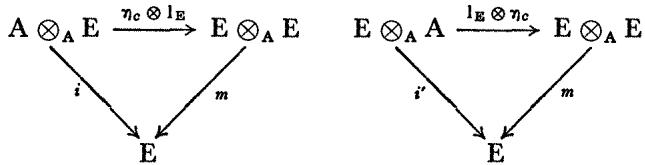
\includegraphics[keepaspectratio]{images/part003_ee0531f1.jpg}}

be commutative (i and i' denoting the canonical isomorphisms (II, §3, no. 4, Proposition 4)).

Let E be an A-algebra with unit element e and let \(\eta = \eta_{e}\) (also denoted by \(\eta_{E}\) ); then \(\eta(\alpha\beta) = \eta(\alpha)\eta(\beta) = \alpha\eta(\beta)\) , for by (2) (no. 1),

\[
(\alpha e) (\beta e) = (\alpha \beta) e = \alpha (\beta e);
\]

hence \(\eta\) is an A-algebra homomorphism. Observe that the A-module structure on E can be defined using \(\eta\) , for

\[
\alpha x = \eta (\alpha). x \quad \text { for } \alpha \in \mathrm{A}, x \in \mathrm{E}\tag{3}
\]

(where, on the right hand side, multiplication is in E). The image of the homomorphism \(\eta\) is a subalgebra of E whose elements commute with all those of E. The kernel of the homomorphism \(\eta\) is the annihilator of the element \(e\) of the A-module E; by (3), it is also the annihilator of the A-module E (II, § 1, no. 12).

When the algebra E is unital and associative, \(\eta\) is a ring homomorphism. Conversely, let \(\rho:A\to B\) be a ring homomorphism such that the image \(\rho(A)\) is contained in the centre of B, assuming also that the ring A is commutative; then an A-algebra structure is defined on B which is associative and unital, by writing (cf.~(3))

\[
\lambda x = \rho (\lambda). x \quad \text { for } \lambda \in \mathbf {A}, x \in \mathbf {E}.
\]

\subsection{PRODUCTS OF ALGEBRAS}

Let \((\mathbf{E}_i)_{i\in I}\) be a family of algebras over the same commutative ring A. It is immediately verified that on the product set \(\mathbf{E} = \prod_{i\in I}\mathbf{E}_i\) , the product A-module structure (II, § 1, no. 5) and the multiplication

\[
\left(\left(x _ {i}\right), \left(y _ {i}\right)\right) \mapsto \left(x _ {i} y _ {i}\right)\tag{4}
\]

define an A-algebra structure; with this structure, the set E is called the product algebra of the family of algebras \((\mathbf{E}_{i})_{i\in I}\) .

When all the algebras \(E_{t}\) are associative (resp. commutative, resp. unital), so is their product. Moreover, all the properties stated in I, §8, no. 10, extend without modification to arbitrary products of algebras.

\subsection{RESTRICTION AND EXTENSION OF SCALARS}

Let \(A_{0}\) and A be two commutative rings and \(\rho:A_{0}\to A\) a ring homomorphism. If E is an A-algebra, we denote (conforming with II, § 1, no. 13) by \(\rho_{*}(E)\) the \(A_{0}\) -module defined by addition on E and the external law

\[
\lambda . x = \rho (\lambda) x \quad \text { for   all } \lambda \in A _ {0} \text { and   all } x \in E.
\]

Multiplication in E and the \(A_{0}\) -module structure on \(\rho_{*}(E)\) define an \(A_{0}\) -algebra structure on \(\rho_{*}(E)\) . When \(A_{0}\) is a subring of A and \(\rho\) the canonical injection, the algebra \(\rho_{*}(E)\) is said to be obtained from E by restricting the ring A of scalars to \(A_{0}\) . By an abuse of language, this is also sometimes said when \(\rho\) is arbitrary.

Let F be an \(A_{0}\) -algebra. An \(A_{0}\) -algebra homomorphism \(F \to \rho_{*}(E)\) is called a semi-homomorphism (relative to \(\rho\) ) or a \(\rho\) -homomorphism of F into the A-algebra E; it is also called an \(A_{0}\) -homomorphism if no confusion arises. If E, \(E'\) are two A-algebras, every A-algebra homomorphism \(E \to E'\) is also an \(A_{0}\) -algebra homomorphism \(\rho_{*}(E) \to \rho_{*}(E')\) .

Consider now two commutative rings A and B and a ring homomorphism \(\rho: \mathbf{A} \to \mathbf{B}\) . For every A-module E, the B-module \(\rho^{*}(\mathbf{E}) = \mathbf{E} \otimes_{\mathbf{A}} \mathbf{B}\) , obtained from E by extending the ring A of scalars to B, has been defined (II, § 5, no. 1). If E is also an A-algebra, we shall define on \(\rho^{*}(\mathbf{E})\) a B-algebra structure. For this, observe that \((\mathbf{E} \otimes_{\mathbf{A}} \mathbf{B}) \otimes_{\mathbf{B}} (\mathbf{E} \otimes_{\mathbf{A}} \mathbf{B})\) is canonically isomorphic to \((\mathbf{E} \otimes_{\mathbf{A}} \mathbf{E}) \otimes_{\mathbf{A}} \mathbf{B}\) (II, § 5, no. 1, Proposition 3). If \(m: \mathbf{E} \otimes_{\mathbf{A}} \mathbf{E} \to \mathbf{E}\) defines the multiplication on E, the mapping \(m \otimes l_{\mathbf{B}}: (\mathbf{E} \otimes_{\mathbf{A}} \mathbf{E}) \otimes_{\mathbf{A}} \mathbf{B} \to \mathbf{E} \otimes_{\mathbf{A}} \mathbf{B}\) is therefore canonically identified with a B-linear mapping

\[
m ^ {\prime}: \rho^ {*} (\mathbf {E}) \otimes_ {\mathbf {B}} \rho^ {*} (\mathbf {E}) \rightarrow \rho^ {*} (\mathbf {E})
\]

which defines the desired B-algebra structure on \(\rho^{*}(\mathbf{E})\) . Hence

\[
(x \otimes \beta) (x ^ {\prime} \otimes \beta^ {\prime}) = (x x ^ {\prime}) \otimes (\beta \beta^ {\prime})\tag{5}
\]

for \(x, x'\) in \(\mathbf{E}\) , \(\beta\) and \(\beta'\) in \(\mathbf{B}\) . The B-algebra \(\rho^*(\mathbf{E})\) is said to be derived from the A-algebra \(\mathbf{E}\) by extending the ring \(\mathbf{A}\) of scalars to \(\mathbf{B}\) (by means of \(\rho\) ). It is also denoted by \(\mathrm{E}_{(\mathbf{B})}\) or \(\mathbf{E} \otimes_{\mathbf{A}} \mathbf{B}\) . When \(\mathbf{E}\) is associative (resp. commutative, resp. unital), so is \(\rho^*(\mathbf{E})\) .

PROPOSITION 1. For every A-algebra E, the canonical mapping \(\phi_{\mathbf{E}}: x \mapsto x \otimes 1\) of E into \(\mathrm{E}_{(\mathbf{B})}\) is an A-homomorphism of algebras. Moreover, for every B-algebra F and every A-homomorphism \(f: \mathbf{E} \to \mathbf{F}\) , there exists one and only one B-homomorphism \(\bar{f}: \mathbf{E}_{(\mathbf{B})} \to \mathbf{F}\) such that \(\bar{f}(x \otimes 1) = f(x)\) for all \(x \in \mathbf{E}\) .

The first assertion follows immediately from the definition of multiplication in \(\mathrm{E}_{(\mathrm{B})}\) , which gives \((x\otimes1)(x'\otimes1)=(xx')\otimes1\) for \(x\in E\) and \(x'\in E\) . The existence and uniqueness of the B-linear mapping \(\bar{f}\) of \(\mathrm{E}_{(\mathrm{B})}\) into F satisfying the relation \(\bar{f}(x\otimes1)=f(x)\) for all \(x\in E\) follow from II, §5, no. 1, Proposition 1; here it all amounts to verifying that \(\bar{f}(yy')=\bar{f}(y)\bar{f}(y')\) for y and \(y'\) in \(\mathrm{E}_{(\mathrm{B})}\) ; as the elements of the form \(x\otimes1\) (with \(x\in E\) ) generate the B-module \(\mathrm{E}_{(\mathrm{B})}\) , attention may be confined to the case where \(y=x\otimes1\) , \(y'=x'\otimes1\) with \(x\in E\) , \(x'\in E\) ; as \(yy'=(xx')\otimes1\) , the relation \(\bar{f}(yy')=\bar{f}(y)\bar{f}(y')\) then follows from \(f(xx')=f(x)f(x')\) .

It can also be said that \(f \mapsto \bar{f}\) is a canonical bijection

\[
\operatorname{Hom} _ {\mathrm{A-alg.}} (\mathrm{E}, \rho_ {*} (\mathrm{F})) \rightarrow \operatorname{Hom} _ {\mathrm{B-alg.}} (\rho^ {*} (\mathrm{E}), \mathrm{F}).\tag{6}
\]

The ordered pair consisting of \(E_{(B)}\) and \(\phi_{E}\) is therefore a solution of the universal mapping problem (Set Theory, IV, §3, no. 1) where \(\Sigma\) is the species of B-algebra structure and the \(\alpha\) -mappings the A-homomorphisms from E to a B-algebra.

COROLLARY. Let E, E' be two A-algebras; for every A-homomorphism of algebras \(u: E \to E'\) , \(u \otimes l_{B}\) is the unique B-homomorphism of algebras v: \(E \otimes_{A} B \to E' \otimes_{A} B\) rendering commutative the diagram

\[
\begin{array}{c} \mathrm{E} \xrightarrow {\phi_ {\mathrm{E}}} \mathrm{E} \otimes_ {\mathrm{A}} \mathrm{B} \\ u \Biggl \downarrow \\ \mathrm{E} ^ {\prime} \xrightarrow [ \phi_ {\mathrm{E} ^ {\prime}} ]{} \mathrm{E} ^ {\prime} \otimes_ {\mathrm{A}} \mathrm{B} \end{array}
\]

Let C be a third commutative ring and \(\sigma: B \to C\) a ring homomorphism; it is immediate that the canonical C-homomorphism

\[
\sigma^ {*} (\rho^ {*} (\mathbf {E})) \rightarrow (\sigma \circ \rho) ^ {*} (\mathbf {E})
\]

mapping \((x\otimes 1)\otimes 1\) to \(x\otimes 1\) for all \(x\in \mathbf{E}\) (II, §5, no. 1, Proposition 2) is an algebra isomorphism.

\subsection{INVERSE AND DIRECT LIMITS OF ALGEBRAS}

Let I be a preordered set and \((\mathbf{A}_{i},\phi_{ij})\) an inverse system of commutative rings with I as indexing set. Let \((\mathbf{E}_{i},f_{ij})\) be an inverse system of \(A_{i}\) -modules with I as indexing set (II, §6, no. 1) and suppose further that each \(E_{i}\) has an \(A_{i}\) -algebra structure and that, for \(i\leqslant j,f_{ij}\) is an \(A_{j}\) -homomorphism of algebras (relative to \(\phi_{ij}\) ) (no. 5). Let \(A=\varprojlim A_{i}\) and \(E=\varprojlim E_{i}\) , which has an A-module structure, the inverse limit of the structure of the \(\mathbf{A}_i\) -modules \(\mathbf{E}_i\) (II, §6, no. 1); it is immediately verified that the law of composition on \(\mathbf{E}\) , considered as the inverse limit of the \(\mathbf{E}_i\) considered as magmas under multiplication (I, §10, no. 1), with the A-module structure on \(\mathbf{E}\) , defines on \(\mathbf{E}\) an A-algebra structure; \((\mathbf{E}_i, f_{ij})\) is called an inverse system of \(\mathbf{A}_i\) -algebras and the A-algebra \(\mathbf{E}\) is called its inverse limit. If \(f_i: \mathbf{E} \to \mathbf{E}_i\) , \(\phi_i: \mathbf{A} \to \mathbf{A}_i\) are the canonical mappings, \(f_i\) is an A-homomorphism of algebras (relative to \(\phi_i\) ). If the \(\mathbf{E}_i\) are associative (resp. commutative), so is \(\mathbf{E}\) ; if each \(\mathbf{E}_i\) admits a unit element \(e_i\) and \(f_{ij}(e_j) = e_i\) for \(i \leqslant j\) , \(e = (e_i)\) is a unit element of the algebra \(\mathbf{E}\) .

Let \((\mathbf{E}_{i}^{\prime}, f_{ij}^{\prime})\) be another inverse system of \(A_{i}\) -algebras and for all i let \(u_{i}: E_{i} \to E_{i}^{\prime}\) be an \(A_{i}\) -algebra homomorphism, these mappings forming an inverse system; then \(u = \lim u_{i}\) is an A-algebra homomorphism.

Suppose now that all the \(A_{i}\) are equal to the same commutative ring A and the \(\phi_{ij}\) to \(Id_{A}\) , so that \(E = \lim E_{i}\) is an A-algebra. Let F be an A-algebra and, for all \(i \in I\) , let \(u_{i}: F \to E_{i}\) be an A-algebra homomorphism such that \((u_{i})\) is an inverse system of mappings; then \(u = \lim u_{i}\) is a homomorphism of the algebra F into the algebra E. Conversely, for every A-algebra homomorphism \(v: F \to E\) , the family of \(v_{i} = f_{i} \circ v\) is an inverse system of A-algebra homomorphisms such that \(v = \lim v_{i}\) . As moreover, writing \(\bar{f}_{ij} = \text{Hom}(1_{\text{F}}, f_{ij})\) , \((\text{Hom}_{\text{A-alg.}}(\text{F}, \text{E}_i), \bar{f}_{ij})\) is clearly an inverse system of sets, it is seen that the above remarks can also be expressed by saying that the canonical mapping \(v \mapsto (f_i \circ v)\) is a bijection

\[
l _ {\mathrm{F}}: \operatorname{Hom} _ {\mathrm{A-alg.}} (\mathrm{F}, \varprojlim \mathrm{E} _ {i}) \rightarrow \varprojlim \operatorname{Hom} _ {\mathrm{A-alg.}} (\mathrm{F}, \mathrm{E} _ {i}).
\]

Moreover, for every A-algebra homomorphism \(w: \mathbf{F} \to \mathbf{F}'\) , the

\[
\bar {w} _ {i} = \operatorname{Hom} (w, 1 _ {\mathrm{E} _ {i}}): \operatorname{Hom} _ {\mathrm{A-alg.}} (\mathrm{F} ^ {\prime}, \mathrm{E} _ {i}) \rightarrow \operatorname{Hom} _ {\mathrm{A-alg.}} (\mathrm{F}, \mathrm{E} _ {i})
\]

form an inverse system of mappings and the diagram

\[
\begin{array}{c} \operatorname{Hom} _ {\mathrm{A-alg.}} (\mathrm{F} ^ {\prime}, \lim \mathrm{E} _ {i}) \xrightarrow {l _ {\mathbf {F} ^ {\prime}}} \lim \operatorname{Hom} _ {\mathrm{A-alg.}} (\mathrm{F} ^ {\prime}, \mathrm{E} _ {i}) \\ \operatorname{Hom} (w, 1 _ {\mathbf {E}}) \Biggl \downarrow \qquad \qquad \qquad \qquad \qquad \qquad \qquad \qquad \qquad \qquad \qquad \qquad \qquad \qquad \qquad \qquad \qquad \qquad \qquad \qquad \qquad \qquad \qquad \qquad \qquad \qquad \qquad \qquad \qquad \qquad \qquad \qquad \qquad \qquad \\ \operatorname{Hom} _ {\mathrm{A-alg.}} (\mathrm{F}, \lim \mathrm{E} _ {i}) \xrightarrow {l _ {\mathbf {F}}} \lim \operatorname{Hom} _ {\mathrm{A-alg.}} (\mathrm{F}, \mathrm{E} _ {i}) \end{array}
\]

is commutative.

Suppose now that I is right directed. Consider a direct system of commutative rings \((\mathbf{A}_i, \phi_{ji})\) and a direct system \((\mathbf{E}_i, f_{ji})\) of \(\mathbf{A}_i\) -modules, with I as indexing set; suppose that each \(\mathbf{E}_i\) has an \(\mathbf{A}_i\) -algebra structure and that, for \(i \leqslant j\) , \(f_{ji}\) is an \(\mathbf{A}_i\) -homomorphism of algebras (relative to \(\phi_{ji}\) ) (no. 5). Let \(\mathbf{A} = \varinjlim \mathbf{A}_i\) , \(\mathbf{E} = \varinjlim \mathbf{E}_i\) ; \(\mathbf{E}\) has an A-module structure, the direct limit of the structures of the \(\mathbf{A}_i\) -modules \(\mathbf{E}_i\) (II, §6, no. 2); moreover, the law of composition on E considered as the direct limit of the \(E_{i}\) , considered as magmas under multiplication (I, §10, no. 3), with the A-module structure on E, defines an A-algebra structure on E; \((\mathbf{E}_{i}, f_{jt})\) is called a direct system of \(A_{i}\) -algebras and the A-algebra E is called its direct limit. If \(f_{i}: E_{i} \to E\) , \(\phi_{i}: A_{i} \to A\) are the canonical mappings, \(f_{i}\) is an \(A_{i}\) -homomorphism of algebras (relative to \(\phi_{i}\) ). If the \(E_{i}\) are associative (resp. commutative), so is E; if each \(E_{i}\) admits a unit element \(e_{i}\) and \(f_{jt}(e_{i}) = e_{j}\) for \(i \leqslant j\) , E admits a unit element e such that \(f_{i}(e_{i}) = e\) for all \(i \in I\) .

Let \((\mathbf{E}_i', f_{ji}')\) be another direct system of \(\mathbf{A}_i\) -algebras and for all \(i\) let \(u_i: \mathbf{E}_i \to \mathbf{E}_i'\) be an \(\mathbf{A}_i\) -algebra homomorphism, these mappings forming a direct system; then \(u = \lim u_i\) is an \(\mathbf{A}\) -algebra homomorphism.

Suppose now that all the rings \(\mathbf{A}_i\) are equal to the same ring \(\mathbf{A}\) and the \(\phi_{ji}\) to \(\mathrm{Id}_{\mathbf{A}}\) , so that \(\mathbf{E} = \varinjlim \mathbf{E}_i\) is an A-algebra. Let \(\mathbf{F}\) be an A-algebra and for all \(i\) let \(u_i: \mathbf{E}_i \to \mathbf{F}\) an A-algebra homomorphism such that \((u_i)\) is a direct system of mappings; then \(u = \varinjlim u_i\) is a homomorphism of the algebra \(\mathbf{E}\) into the algebra \(\mathbf{F}\) . Conversely, for every A-algebra homomorphism \(v: \mathbf{E} \to \mathbf{F}\) , the family of \(v_i = v \circ f_i\) is a direct system of A-algebra homomorphisms such that \(v = \varinjlim v_i\) . As moreover, writing \(\bar{f}_{ij} = \operatorname{Hom}(f_{ij}, 1_F)\) , \((\operatorname{Hom}_{\mathbf{A-alg}}(\mathbf{E}_i, \mathbf{F}), \bar{f}_{ij})\) is clearly an inverse system of sets, it is seen that the above remarks can also be expressed by saying that the canonical mapping \(v \mapsto (v \circ f_i)\) is a bijection

\[
d _ {\mathrm{F}}: \operatorname{Hom} _ {\mathrm{A-alg.}} (\varinjlim \mathrm{E} _ {i}, \mathrm{F}) \rightarrow \varprojlim \operatorname{Hom} _ {\mathrm{A-alg.}} (\mathrm{E} _ {i}, \mathrm{F}).
\]

Further, for every A-algebra homomorphism \(w: F \rightarrow F'\) , the

\[
\bar {w} _ {i} = \operatorname{Hom} (1 _ {\mathrm{E} _ {i}}, w): \operatorname{Hom} _ {\mathrm{A-alg.}} (\mathrm{E} _ {i}, \mathrm{F}) \rightarrow \operatorname{Hom} _ {\mathrm{A-alg.}} (\mathrm{E} _ {i}, \mathrm{F} ^ {\prime})
\]

form an inverse system of mappings and the diagram

\[
\begin{array}{l} \operatorname{Hom} _ {\mathrm{A-alg.}} (\varinjlim \mathrm{E} _ {i}, \mathrm{F}) \xrightarrow {d _ {\mathrm{F}}} \varprojlim \operatorname{Hom} _ {\mathrm{A-alg.}} (\mathrm{E} _ {i}, \mathrm{F}) \\ \operatorname{Hom} (1 _ {\mathrm{E}}, w) \Biggl \downarrow \qquad \qquad \qquad \qquad \qquad \qquad \qquad \qquad \qquad \qquad \qquad \qquad \qquad \qquad \qquad \qquad \qquad \qquad \qquad \qquad \varprojlim \varpi_ {i} \\ \operatorname{Hom} _ {\mathrm{A-alg.}} (\varinjlim \mathrm{E} _ {i}, \mathrm{F} ^ {\prime}) \xrightarrow {d _ {\mathrm{F} ^ {\prime}}} \varprojlim \operatorname{Hom} _ {\mathrm{A-alg.}} (\mathrm{E} _ {i}, \mathrm{F} ^ {\prime}) \end{array}
\]

is commutative.

\subsection{BASES OF AN ALGEBRA. MULTIPLICATION TABLE}

By definition, a basis of an A-algebra E is a basis of E for its A-module structure. Let \((a_{i})_{i\in I}\) be a basis of E; there exists a unique family \((\gamma_{ij}^{k})_{(i,j,k)\in I\times I\times I}\) of elements of the ring A such that for every ordered pair \((i,j)\in I\times I\) , the set of \(k\in I\) such that \(\gamma_{ij}^{k}\neq 0\) is finite and

\[
a _ {i} a _ {j} = \sum_ {k \in \mathbf {I}} \gamma_ {i j} ^ {k} a _ {k}.\tag{7}
\]

The \(\gamma_{ij}^{k}\) are called the constants of structure of the algebra E with respect to the basis \((a_{i})\) and relations (7) constitute the multiplication table of the algebra E (relative to the basis \((a_{i})\) ).

Relations (7) can be imagined written down by setting out the right hand sides of these relations in a square table

\(\cdots\)

\(a_j\)

\(\cdots\)

\(\vdots\)

\(a_j\)

\(\sum_{k} \gamma_{ij}^{k} a_k\)

\(\vdots\)

it being understood that the element appearing in the row of index i and the column of index j is equal to the product \(a_{i}a_{j}\) .

Conversely, given an A-module E, a basis \((a_{i})_{i\in I}\) of E and a family \((\gamma_{ij}^{k})\) of elements of A such that for every ordered pair \((i,j)\in I\times I\) the set of \(k\in I\) such that \(\gamma_{ij}^{k}\neq 0\) is finite, then there is on E one and only one A-algebra structure under which relations (7) hold, since the A-module \(\mathbf{E}\otimes_{\mathbf{A}}\mathbf{E}\) is free and admits as basis \((a_{i}\otimes a_{j})_{(i,j)\in I\times I}\) (cf.~II, § 3, no. 7, Corollary 2 to Proposition 7).

Let E be an A-algebra and \((a_{i})_{i\in I}\) a generating system of the A-module E (for example a basis). For E to be associative, it is necessary and sufficient that the \(a_{i}\) satisfy the associativity relations

\[
(a _ {i} a _ {j}) a _ {k} = a _ {i} (a _ {j} a _ {k}) \quad \text { for   all } i, j, k\tag{8}
\]

The mapping \((x, y, z) \mapsto (xy)z - x(yz)\) is an A-trilinear mapping

\[
\mathbf {E} \times \mathbf {E} \times \mathbf {E} \rightarrow \mathbf {E}
\]

and hence defines an A-linear mapping \(E \otimes_{A} E \otimes_{A} E \to E\) ; if the latter mapping is zero for all the elements \(a_{i} \otimes a_{j} \otimes a_{k}\) , which form a generating system of the A-module \(E \otimes_{A} E \otimes_{A} E\) , it is identically zero.

Similarly, for E to be commutative, it is necessary and sufficient that the \(a_{i}\) satisfy the commutativity relations

\[
a _ {i} a _ {j} = a _ {j} a _ {i} \quad \text { for   all } i, j.\tag{9}
\]

The proof is analogous, this time considering the A-bilinear mapping \((x,y)\mapsto xy - yx\) . Finally, for an element \(e\in E\) to be a unit element, it is necessary and sufficient that the \(a_{i}\) satisfy the relations

\[
a _ {i} = e a _ {i} = a _ {i} e \quad \text { for   all } i,\tag{10}
\]

as is seen this time by considering the A-linear mappings \(x \mapsto x - xe\) and \(x \mapsto x - ex\) .

When \((a_{i})_{i\in I}\) is a basis of E and \((\gamma_{ij}^{k})\) the corresponding family of constants of structure, relations (8) are equivalent to the relations

\[
\sum_ {r} \gamma_ {i j} ^ {r} \gamma_ {r k} ^ {s} = \sum_ {r} \gamma_ {i r} ^ {s} \gamma_ {j k} ^ {r}
\]

for all \(i, j, k, s\) . Similarly relations (9) are equivalent to \(\gamma_{ij}^{k} = \gamma_{ji}^{k}\) for all \(i, j, k\) .

Let \((a_{i})_{i\in I}\) be a basis of the A-algebra E; if \(\rho :A\to B\) is a ring homomorphism, \((a_{i}\otimes 1)\) is a basis of the B-algebra \(\rho^{*}(\mathbf{E}) = \mathbf{E}\otimes_{\mathbf{A}}\mathbf{B}\) (II, §5, no. 1, Proposition 4). If \((\gamma_{ij}^{k})\) is the family of constants of structure relative to the basis \((a_{i})\) , the family \((\rho (\gamma_{ij}^{k}))\) is the family of constants of structure of \(\rho^{*}(\mathbf{E})\) relative to the basis \((a_{i}\otimes 1)\) .

\section{EXAMPLES OF ALGEBRAS}

Throughout this paragraph, A denotes a commutative ring.

\subsection{ENDOMORPHISM ALGEBRAS}

Let B be an associative A-algebra with a unit element denoted by 1 and let M be a right B-module. We know that the ring \(\mathbf{E} = \operatorname{End}_{\mathbf{B}}(\mathbf{M})\) also has a module structure over the centre of B. Now the image of the homomorphism \(h: \alpha \mapsto \alpha\) . 1 of A into B is contained in the centre of B ( \(\S 1\) , no. 1); hence \(h\) gives E an A-module structure. Further, for \(\alpha \in \mathbf{A}\) and \(f, g\) in E,

\[
\alpha (f \circ g) = f \circ (\alpha g) = (\alpha f) \circ g;
\]

hence multiplication in E and the A-module structure on E define an associative A-algebra structure on E; the identity mapping of M is a unit element of this algebra.

\subsection{MATRIX ELEMENTS}

Let B be a unital associative A-algebra and \(\mathbf{M}_{n}(\mathrm{B})\) the set of square matrix of order n over B (II, § 10, no. 7). Then \(\mathbf{M}_{n}(\mathrm{B})\) has an A-module structure defined by \(\alpha.(b_{ij})=(\alpha b_{ij})(\alpha\in\mathrm{A},b_{ij}\in\mathrm{B},1\leqslant i\leqslant n,1\leqslant j\leqslant n)\) ; this structure and matrix multiplication define a unital associative A-algebra structure on \(\mathbf{M}_{n}(\mathrm{B})\) . The canonical bijection of \(\mathbf{M}_{n}(\mathrm{B})\) onto \(\operatorname{End}_{\mathrm{B}}(\mathrm{B}_{d}^{n})\) (II, § 10, no. 7) is an A-algebra isomorphism.

When B = A, the A-algebra \(\mathbf{M}_{n}(\mathbf{A})\) admits a canonical basis \((E_{ij})\) consisting of the matrix units (II, §10, no. 3); the corresponding multiplication table is

\[
E _ {i j} E _ {h k} = \delta_ {j h} \mathrm{E} _ {i k}.\tag{1}
\]

The unit element \(I_{n}\) is equal to \(\sum_{i=1}^{n} E_{ii}\) .

\subsection{QUADRATIC ALGEBRAS}

Let \(\alpha, \beta\) be two elements of A and \((e_1, e_2)\) the canonical basis of \(\mathbf{A}^2\) . The quadratic algebra of type \((\alpha, \beta)\) over A is the A-module \(\mathbf{A}^2\) with the algebra structure defined by the multiplication table (§ 1, no. 7)

\[
e _ {1} ^ {2} = e _ {1}, \qquad e _ {1} e _ {2} = e _ {2} e _ {1} = e _ {2}, \qquad e _ {2} ^ {2} = \alpha e _ {1} + \beta e _ {2}.\tag{2}
\]

An A-algebra E isomorphic to a quadratic algebra is also called a quadratic algebra. It amounts to the same to say that E admits a basis of two elements one of which is the unit element.

It can be shown that every unital A-algebra which admits a basis of two elements is a quadratic algebra (Exercise 1).

If a basis \((e_{1}, e_{2})\) of an A-algebra has multiplication table (2), it is called a basis of type \((\alpha, \beta)\) . By an abuse of language, a quadratic algebra is said to be of type \((\alpha, \beta)\) when it has a basis of type \((\alpha, \beta)\) .

PROPOSITION 1. A quadratic algebra E is associative and commutative.

The fact that E is commutative follows from the equation \(e_{1}e_{2}=e_{2}e_{1}\) in (2); similarly, to verify associativity, it suffices to see that \(x(yz)=(xy)z\) when x,y,z are each equal to \(e_{1}\) or \(e_{2}\) . Now, this relation is obvious if at least one of the elements x,y,z is equal to \(e_{1}\) ; it is also true for x=y=z=e₂ since E is commutative; whence the proposition.

Let \(e\) denote the unit element of a quadratic algebra \(\mathbf{E}\) and let \((e, i)\) be a basis of \(\mathbf{E}\) of type \((\alpha, \beta)\) ; every other basis of \(\mathbf{E}\) containing \(e\) is therefore of the form \((e, j)\) with \(j = \gamma e + \delta i\) (II, §7, no. 2, Corollary to Proposition 3); moreover, for \((e, j)\) to be a basis of \(\mathbf{E}\) , it is necessary and sufficient that \(\delta\) be invertible in \(\mathbf{A}\) ; the condition is obviously sufficient; conversely, if \(i\) is the canonical image of \(i\) in \(\mathbf{E}/\mathbf{A}e\) , \(i\) and \(\bar{j} = \delta i\) must each form a basis of \(\mathbf{E}/\mathbf{A}e\) , whence the necessity of the condition. Then

\[
j ^ {2} = (\gamma^ {2} + \alpha \delta^ {2}) e + (2 \gamma \delta + \beta \delta^ {2}) i = (\alpha \delta^ {2} - \gamma^ {2} - \beta \gamma \delta) e + (2 \gamma + \beta \delta) j;
\]

thus it is seen that E is of type

\[
(\alpha \delta^ {2} - \gamma^ {2} - \beta \gamma \delta , 2 \gamma + \beta \delta)\tag{3}
\]

for all invertible \(\delta \in \mathbf{A}\) and all \(\gamma \in \mathbf{A}\) . In particular, if \(\mathbf{E}\) is of type \((\alpha, 2\beta')\) , i is also of type \((\alpha + \beta'^2, 0)\) as is seen by taking \(\gamma = -\beta'\) and \(\delta = 1\) .

PROPOSITION 2. Let E be a quadratic A-algebra and e its unit element. For all \(u \in \mathbf{E}\) , let \(\mathrm{T}(u)\) be the trace of the endomorphism \(m_u: x \mapsto ux\) of the free A-module E (II, §4, no. 3). Then the mapping \(s\) defined by \(s(u) = \mathrm{T}(u)\) . \(e - u\) is an automorphism of the algebra E and \(s^2(u) = u\) for all \(u \in \mathbf{E}\) .

Let \((e, i)\) be a basis of E of type \((\alpha, \beta)\) ; then \(T(e) = 2\) , when \(s(e) = e\) , and \(T(i) = \beta\) , whence \(s(i) = \beta e - i\) . Hence \((e, s(i))\) is a basis of E, whose type is given by (3) with \(\gamma = \beta\) and \(\delta = -1\) , which again gives \((\alpha, \beta)\) ; it follows that \(s\) is an automorphism of the algebra E. As \(m_{s(u)} = sm_u s^{-1}\) , the endomorphisms \(m_u\) and \(m_{s(u)}\) of the A-module E have the same trace (II, §4, no. 3, Proposition 3), whence

\[
s ^ {2} (u) = \mathrm{T} (u). e - s (u) = \mathrm{T} (u). e - (\mathrm{T} (u). e - u) = u
\]

for all \(u \in E\) .

The automorphism \(s\) is called conjugation of the A-algebra \(\mathbf{E}\) and \(s(u)\) the conjugate of \(u\) .

If \(u = \xi e + \eta i\) , with \(\xi, \eta\) in \(A\) , then \(s(u) = (\xi + \beta \eta)e - \eta i\) , whence

\begin{enumerate}
\def\labelenumi{(\arabic{enumi})}
\setcounter{enumi}{3}
\tightlist
\item
\end{enumerate}

\[
\mathrm{T} (u) e = u + s (u) = (2 \xi + \beta \eta) e\tag{5}
\]

\[
u. s (u) = (\xi^ {2} + \beta \xi \eta - \alpha \eta^ {2}) e = N (u) e
\]

where we have written \(\mathrm{N}(u)=\xi^{2}+\beta\xi\eta-\alpha\eta^{2}\) . The elements \(\mathrm{T}(u)\) and \(\mathrm{N}(u)\) (or, when A and Ae are canonically identified, the elements \(\mathrm{T}(u)e\) and \(\mathrm{N}(u)e\) ) are called respectively the trace and norm of u.

When \(\beta = 0\) , the above formulae are simplified to

\[
s (\xi e + \eta i) = \xi e - \eta i, \quad \mathrm{T} (\xi e + \eta i) = 2 \xi , \quad \mathrm{N} (\xi e + \eta i) = \xi^ {2} - \alpha \eta^ {2}. \tag {6}
\]

Clearly T is a linear form on E and N is a quadratic form on E (IX, § 3, no. 4). As E is commutative and associative, it follows from (5) that

\[
\mathrm{N} (u v) = \mathrm{N} (u)) \mathrm{N} (v).\tag{7}
\]

For u to be invertible in E, it is necessary and sufficient that \(\mathrm{N}(u)\) be invertible in A. For, as \(\mathrm{N}(e)=1\) , the necessity of the condition follows from (7), writing \(v=u^{-1}\) . Conversely, if \(\mathrm{N}(u)\) is invertible in A, it follows from (5) that u is invertible and that

\[
u ^ {- 1} = (\mathrm{N} (u)) ^ {- 1} s (u).\tag{8}
\]

It can be proved that \(\mathbf{N}(u)\) is the determinant (§ 8, no. 1) of the endomorphism \(m_u\) (cf.~§ 9 no. 3, Example 1).

The following proposition gives the structure of quadratic algebras over a commutative field:

PROPOSITION 3. Let E be a quadratic A-algebra of type \((\alpha, \beta)\) .

\begin{enumerate}
\def\labelenumi{(\roman{enumi})}
\item
  If \(\mathbf{A}\) is a field and contains no element \(\zeta\) such that \(\zeta^2 = \alpha + \beta \zeta\) , \(\mathbf{E}\) is \(a\) (commutative) field (cf.~V, § 3).
\item
  If the ring A contains an element \(\zeta\) such that \(\zeta^2 = \alpha + \beta\zeta\) and \(\beta - 2\zeta\) is invertible (resp. zero), E is isomorphic to \(\mathbf{A} \times \mathbf{A}\) (resp. is of type \((0,0)\) ).
\end{enumerate}

We prove (i). Let \(\xi, \eta\) be two elements of A and \(u = \xi e + \eta i\) . If \(\eta \neq 0\) and we write \(\theta = -\xi \eta^{-1}\) , then \(\mathrm{N}(u) = \eta^2 (\theta^2 - \beta \theta - \alpha)\) by (5), whence \(\mathrm{N}(u) \neq 0\) by virtue of the hypothesis on A; if \(\eta = 0\) , then \(\mathrm{N}(u) = \xi^2\) . In any case, if \(u \neq 0\) , then \(\mathrm{N}(u) \neq 0\) , hence \(\mathrm{N}(u)\) is invertible in A and therefore \(u\) is invertible in E.

We now prove (ii). The canonical basis \((e_{1}, e_{2})\) of the algebra \(A \times A\) is of type \((0, 1)\) . We have seen (formula (3)) that E is of type

\[
(\alpha \delta^ {2} - \gamma^ {2} - \beta \gamma \delta , 2 \gamma + \beta \delta)
\]

for all \(\gamma \in \mathbf{A}\) and all \(\delta\) invertible in \(\mathbf{A}\) . If \(\beta - 2\zeta\) is invertible, take \(\delta = (\beta - 2\zeta)^{-1}\) and \(\gamma = -\zeta(\beta - 2\zeta)^{-1}\) ; then \(2\gamma + \beta\delta = 1\) and

\[
\alpha \delta^ {2} - \gamma^ {2} - \beta \gamma \delta = \delta^ {2} (\alpha - \zeta^ {2} + \beta \zeta) = 0;
\]

thus E is of type \((0,1)\) and hence isomorphic to A × A. If \(\beta - 2\zeta = 0\) , it has already been remarked that E is of type \((\alpha + \zeta^{2}, 0)\) and hence of type \((0,0)\) since \(\alpha + \zeta^{2} = 2\zeta^{2} - \beta\zeta = 0\) .

A quadratic A-algebra of type \((0,0)\) is also called an algebra of dual numbers over A.

\subsection{CAYLEY ALGEBRAS}

DEFINITION 1. A Cayley algebra over \(\mathbf{A}\) is an ordered pair \((\mathbf{E}, s)\) , where \(\mathbf{E}\) is an algebra over \(\mathbf{A}\) with a unit element \(e\) and \(s\) is an antiautomorphism of \(\mathbf{E}\) such that

\[
u + s (u) \in \mathrm{A} e \quad \text { and } \quad u. s (u) \in \mathrm{A} e
\]

for all \(u \in \mathbf{E}\) .

s is called the conjugation of the Cayley algebra (E, s) and \(s(u)\) the conjugate of u. The condition \(u + s(u) \in Ae\) implies that u and \(s(u)\) are permutable. We write

\begin{enumerate}
\def\labelenumi{(\arabic{enumi})}
\setcounter{enumi}{8}
\tightlist
\item
\end{enumerate}

\[
\mathrm{T} (u) = u + s (u)\tag{10}
\]

\[
\mathrm{N} (u) = u. s (u) = s (u). u
\]

and these elements of the subalgebra Ae are called respectively the Cayley trace and norm of u.

The ordered pair consisting of a quadratic algebra E and its conjugation s (which is an antiautomorphism since E is commutative) (no. 3) is a Cayley algebra.

Let \((\mathbf{E}, s)\) be a Cayley algebra; as \(s(e) = e\) , \(s(u + s(u)) = u + s(u)\) , in other words \(s(u) + s^2(u) = u + s(u)\) or also

\[
s ^ {2} (u) = u\tag{11}
\]

so that \(s^{2}\) is the identity mapping of E. It follows that

\[
\mathrm{T} (s (u)) = \mathrm{T} (u), \quad \mathrm{N} (s (u)) = \mathrm{N} (u).\tag{12}
\]

Finally, the relation \((u - u)(u - s(u)) = 0\) gives

\[
u ^ {2} - \mathrm{T} (u). u + \mathrm{N} (u) = 0\tag{13}
\]

for all \(u \in \mathbf{E}\) .

PROPOSITION 4. Let E be an A-algebra and s and \(s'\) antiautomorphisms of E such that \((E, s)\) and \((E, s')\) are Cayley algebras. If E admits a basis containing the unit element e, then \(s' = s\) .

Clearly \(s'(u) = s(u) = u\) for all \(u \in Ae\) . If T, N (resp. T', N') are the trace and norm functions for (E, s) (resp. (E, s')), it follows from (13) that

\[
(\mathrm{T} (u) - \mathrm{T} ^ {\prime} (u)). u - (\mathrm{N} (u) - \mathrm{N} ^ {\prime} (u)) = 0.
\]

Let B be a basis of E containing e and u an element of B distinct from e; then \(\mathrm{T}(u) - \mathrm{T}'(u) = 0\) , whence \(s(u) = s'(u)\) . As s and \(s'\) coincide on B, they are equal.

In what follows, we shall write \(\bar{u} = s(u)\) , so that

\[
\left\{ \begin{array}{l l} u + \bar {u} = \mathrm{T} (u), & u \bar {u} = \bar {u} u = \mathrm{N} (u), \quad \bar {\bar {u}} = u \\ \overline {{u + v}} = \bar {u} + \bar {v}, & \overline {{\alpha u}} = \alpha \bar {u}, \quad \overline {{u v}} = \bar {v}. \bar {u} \end{array} \right.\tag{14}
\]

for \(u, v\) in \(\mathbf{E}, \alpha \in \mathbf{A}\) ; moreover

\[
\mathbf {T} (e) = 2 e, \quad \mathbf {N} (e) = e.\tag{15}
\]

From the formula

\[
\mathrm{T} (u v) = u v + \overline {{{{u v}}}} = u v + \bar {v}. \bar {u} = u v + (\mathrm{T} (v) - v) (\mathrm{T} (u) - u),
\]

we deduce that

\[
u v + v u = \mathrm{T} (u) v + \mathrm{T} (v) u + (\mathrm{T} (u v) - \mathrm{T} (u) \mathrm{T} (v))\tag{16}
\]

whence, exchanging \(u\) and \(v\) ,

\[
\mathbf {T} (v u) = \mathbf {T} (u v).\tag{17}
\]

On the other hand, \(\mathrm{N}(u+v)=(u+v)(\bar{u}+\bar{v})=\mathrm{N}(u)+\mathrm{N}(v)+\mathrm{T}(u\bar{v})\) , whence

\[
\mathrm{T} (v \bar {u}) = \mathrm{T} (u \bar {v}) = \mathrm{N} (u + v) - \mathrm{N} (u) - \mathrm{N} (v).\tag{18}
\]

Now, (16) applied with u replaced by \(\bar{u}\) gives

\[
\mathrm{T} (u \bar {v}) = \mathrm{T} (u) \mathrm{T} (v) + \bar {u} v + v \bar {u} - \mathrm{T} (u) v - \mathrm{T} (v) \bar {u} = \mathrm{T} (u) \mathrm{T} (v) - u v - \bar {v}. \bar {u};
\]

whence

\[
\mathrm{T} (v \bar {u}) = \mathrm{T} (u \bar {v}) = \mathrm{N} (u + v) - \mathrm{N} (u) - \mathrm{N} (v) = \mathrm{T} (u) \mathrm{T} (v) - \mathrm{T} (u v).\tag{19}
\]

Finally, clearly for all \(\alpha \in \mathbf{A}\) ,

\[
\mathrm{N} (\alpha u) = \alpha^ {2} \mathrm{N} (u);\tag{20}
\]

in particular \(\mathbf{N}(2u) = 4\mathbf{N}(u)\) , so that formula (19) gives

\[
(\mathrm{T} (u)) ^ {2} - \mathrm{T} (u ^ {2}) = 2 \mathrm{N} (u).\tag{21}
\]

Clearly T is a linear form on the (Ae)-module E. As \((u, v) \mapsto \mathrm{T}(v\bar{u})\) is a bilinear form on this module, it follows from (18) and (20) that N is a quadratic form (cf.~IX, § 3, no. 4).

\subsection{CONSTRUCTION OF CAYLEY ALGEBRAS. QUATERNIONS}

Let \((\mathbf{E}, s)\) be a Cayley algebra over A, for which we shall use the notation of no. 4, and let \(\gamma \in \mathbf{A}\) . Let F be the algebra over A whose underlying module is \(\mathbf{E} \times \mathbf{E}\) and whose multiplication is defined by

\[
(x, y) (x ^ {\prime}, y ^ {\prime}) = (x x ^ {\prime} + \gamma \bar {y} ^ {\prime} y, y \bar {x} ^ {\prime} + y ^ {\prime} x);\tag{22}
\]

clearly \((e,0)\) is unit element of F and \(E \times \{0\}\) is a subalgebra of F isomorphic to E; we shall identify it with E in what follows, so that \(x \in E\) is identified with \((x,0)\) and in particular e is identified with the unit element of F.

Let \(t\) be the permutation of \(\mathbf{F}\) defined by

\begin{enumerate}
\def\labelenumi{(\arabic{enumi})}
\setcounter{enumi}{22}
\tightlist
\item
\end{enumerate}

\[
t ((x, y)) = (\bar {x}, - y) \quad (x \in \mathbf {E}, y \in \mathbf {E}).
\]

PROPOSITION 5. (i) The ordered pair \((\mathbf{F}, t)\) is a Cayley algebra over \(\mathbf{A}\) .

\begin{enumerate}
\def\labelenumi{(\roman{enumi})}
\setcounter{enumi}{1}
\tightlist
\item
  Let \(j = (0, e)\) , so that \((x, y) = xe + yj\) for \(x \in \mathbf{E}\) , \(y \in \mathbf{E}\) . The Cayley trace and norm \(\mathbf{T}_{\mathbb{F}}\) and \(\mathbf{N}_{\mathbb{F}}\) of \(\mathbf{F}\) are given by the formulae
\end{enumerate}

\[
\mathrm{T} _ {\mathrm{F}} (x e + y j) = \mathrm{T} (x), \quad \mathrm{N} _ {\mathrm{F}} (x e + y j) = \mathrm{N} (x) - \gamma \mathrm{N} (y).\tag{24}
\]

\begin{enumerate}
\def\labelenumi{(\roman{enumi})}
\setcounter{enumi}{2}
\tightlist
\item
  For F to be associative, it is necessary and sufficient that E be associative and commutative.
\end{enumerate}

For \((x,y)\in \mathbf{F},\)

\begin{enumerate}
\def\labelenumi{(\arabic{enumi})}
\setcounter{enumi}{24}
\tightlist
\item
\end{enumerate}

\[
\begin{array}{r l r} & & {(x, y) + t ((x, y)) = (x + \bar {x}, 0) = \mathrm{T} (x) e} \\ & & {(x, y) t ((x, y)) = (x, y) (\bar {x}, - y) = (x \bar {x} - \gamma \bar {y} y, y \bar {\bar {x}} - y x)} \\ & & {= (\mathrm{N} (x) - \gamma \mathrm{N} (y), 0) = (\mathrm{N} (x) - \gamma \mathrm{N} (y)) e.} \end{array}\tag{26}
\]

To prove both (i) and (ii), it therefore suffices to show that t is an antiautomorphism of F. Clearly t is an A-linear bijection. On the other hand,

\[
\begin{array}{r l} t ((x, y) \cdot (x ^ {\prime}, y ^ {\prime})) & = t ((x x ^ {\prime} + \gamma \bar {y} ^ {\prime} y, y \bar {x} ^ {\prime} + y ^ {\prime} x)) = (\bar {x} ^ {\prime} \bar {x} + \gamma \bar {y} y ^ {\prime}, - y \bar {x} - y ^ {\prime} x) \\ & = (\bar {x} ^ {\prime}, - y ^ {\prime}) (\bar {x}, - y) = t ((x ^ {\prime}, y ^ {\prime})) t ((x, y)) \end{array}
\]

and hence \(t\) is an antiautomorphism.

It remains to prove (iii). As E is identified with a subalgebra of F, E may be assumed to be associative. Let \(u = (x, y)\) , \(u' = (x', y')\) , \(u'' = (x'', y'')\) be elements of F. Then

\[
\left\{ \begin{array}{l} (u u ^ {\prime}) u ^ {\prime \prime} = ((x x ^ {\prime} + \gamma \bar {y} ^ {\prime} y) x ^ {\prime \prime} + \gamma \bar {y} ^ {\prime \prime} (\bar {y} x ^ {\prime} + y ^ {\prime} x), \\ \qquad \qquad \qquad \qquad \qquad \qquad \qquad \qquad \qquad \qquad (y \bar {x} ^ {\prime} + y ^ {\prime} x) \bar {x} ^ {\prime \prime} + y ^ {\prime \prime} (x x ^ {\prime} + \gamma \bar {y} ^ {\prime} y)) \\ u (u ^ {\prime} u ^ {\prime \prime}) = (x (x ^ {\prime} x ^ {\prime \prime} + \gamma \bar {y} ^ {\prime \prime} y ^ {\prime}) + (\gamma (x ^ {\prime \prime} \bar {y} ^ {\prime} + \bar {x} ^ {\prime} \bar {y} ^ {\prime \prime}) y, \\ \qquad \qquad \qquad \qquad \qquad \qquad \qquad \qquad \qquad \qquad y (\bar {x} ^ {\prime \prime} \bar {x} ^ {\prime} + \gamma \bar {y} ^ {\prime} y ^ {\prime \prime}) + (y ^ {\prime} \bar {x} ^ {\prime \prime} + y ^ {\prime \prime} x ^ {\prime}) x). \end{array} \right.\tag{27}
\]

Examining these formulae shows that the commutativity of E implies the associativity of F. Conversely, if F is associative, formulae (27) applied with \(y = y' = 0\) , \(x'' = 0\) and \(y'' = e\) give \((0, x'x) = (0, xx')\) , that is \(x'x = xx'\) for all \(x, x'\) in E; thus E is then commutative.

Note also that, in the above notation, for \(x, y\) in \(\mathbf{E}\) ,

\begin{enumerate}
\def\labelenumi{(\arabic{enumi})}
\setcounter{enumi}{27}
\tightlist
\item
\end{enumerate}

\[
\begin{array}{r l} y j = j \overline {{y}}, & x (y j) = (y x) j, \quad (x j) y = (x \overline {{y}}) j, \quad (x j) (y j) = \overline {{y}} x e \\ & j ^ {2} = e. \end{array}\tag{29}
\]

The Cayley algebra \((\mathbf{F}, t)\) is called the Cayley extension of \((\mathbf{E}, s)\) defined by \(\gamma\) .

Examples. (1) If we take \(\mathbf{E} = \mathbf{A}\) (and hence \(s = 1_{\mathbf{A}}\) ), the algebra \(\mathbf{F}\) is a quadratic \(\mathbf{A}\) -algebra with basis \((e,j)\) where \(j^2 = \gamma e\) .

\begin{enumerate}
\def\labelenumi{(\arabic{enumi})}
\setcounter{enumi}{1}
\tightlist
\item
  Take E to be a quadratic algebra of type \((\alpha, \beta)\) , so that the underlying module of E is \(A^{2}\) , with multiplication table (2) (no. 3) for the canonical basis. Take s to be conjugation of E (no. 3, Proposition 2). Then, for all \(\gamma \in A\) , the Cayley extension F of \((E, s)\) defined by \(\gamma\) is called the quaternion algebra of type \((\alpha, \beta, \gamma)\) , which is associative by no. 3, Proposition 1 and Proposition 5 above; its underlying module is \(A^{4}\) and, if \((e, i, j, k)\) denotes the canonical basis of \(A^{4}\) , the corresponding multiplication table is given by
\end{enumerate}

\[
\left\{ \begin{array}{l l} i ^ {2} = \alpha e + \beta i, & i j = k, \qquad i k = \alpha j + \beta k, \\ j i = \beta j - k, & j ^ {2} = \gamma e, \qquad j k = \beta \gamma e - \gamma i, \\ k i = - \alpha j, & k j = \gamma i, \qquad k ^ {2} = - \alpha \gamma e. \end{array} \right.\tag{30}
\]

Further, for \(u = \rho e + \xi i + \eta j + \eta k\) (with \(\rho, \xi, \eta, \zeta\) in A), we have (writing \(\bar{u}\) instead of \(t(u)\) and identifying A with Ae):

\[
\left\{ \begin{array}{c} u = (\rho + \beta \xi) e - \xi i - \eta j - \zeta k \\ \mathrm{T} _ {\mathrm{F}} (u) = 2 \rho + \beta \xi \\ \mathrm{N} _ {\mathrm{F}} (u) = \rho^ {2} + \beta \rho \xi - \alpha \xi^ {2} - \gamma (\eta^ {2} + \beta \eta \zeta - \alpha \zeta^ {2}). \end{array} \right.\tag{31}
\]

Formulae (30) follow from (28) and (29) and formulae (31) from (23) and (24), taking account of the formulae for the quadratic algebra E.

Then, for \(u, v\) in \(\mathbf{F}\) ,

\[
\mathrm{N} _ {\mathrm{F}} (u v) = \mathrm{N} _ {\mathrm{F}} (u) \mathrm{N} _ {\mathrm{F}} (v)\tag{32}
\]

for \(\mathrm{N}_{\mathbb{F}}(uv)=uv.\overline{uv}=uv(\bar{v}.\bar{u})=u(v\bar{v})\bar{u}=(u\bar{u})(v\bar{v})\) by virtue of the associativity and the fact that \(\mathrm{N}_{\mathbb{F}}(u)\) belongs to the centre of F.

An A-algebra isomorphic to a quaternion algebra is also called a quaternion algebra; if a basis of such an algebra has multiplication table (30), it is called a basis of type \((\alpha, \beta, \gamma)\) . By an abuse of language, a quaternion algebra is said to be of type \((\alpha, \beta, \gamma)\) when it has a basis of type \((\alpha, \beta, \gamma)\) .

When \(\beta = 0\) , formulae (30) and (31) simplify to

\[
\left\{ \begin{array}{l l} i ^ {2} = \alpha e, & \quad i j = k, \qquad i k = \alpha j, \\ j i = - k, & \quad j ^ {2} = \gamma e, \qquad j k = - \gamma i, \\ k i = - \alpha i, & \quad k j = \gamma i, \qquad k ^ {2} = - \alpha \gamma e, \end{array} \right.\tag{33}
\]

and

\[
\left\{ \begin{array} {c}\bar {u} = \rho e - \xi i - \eta j - \zeta k \\ \mathrm{T} _ {\mathrm{F}} (u) = 2 \rho \\ \mathrm{N} _ {\mathrm{F}} (u) = \rho^ {2} - \alpha \xi^ {2} - \gamma \eta^ {2} + \alpha \gamma \zeta^ {2}. \\ \end{array} \right.\tag{34}
\]

Then \((\alpha, \beta, \gamma)\) is replaced throughout by \((\alpha, \gamma)\) in the above expressions. It is immediate that the quaternion algebras of types \((\alpha, \gamma)\) and \((\gamma, \alpha)\) are isomorphic.

Note that formulae (32) show that F is not commutative when \(-1 \neq 1\) in A.

Taking A to be the field \(\mathbf{R}\) of real numbers and \(\alpha = \gamma = -1\) , \(\beta = 0\) , the corresponding algebra \(F\) is called the algebra of Hamiltonian quaternions and is denoted by \(\mathbf{H}\) . If \(u = \rho e + \xi i + \eta j + \zeta k\) ( \(\rho, \xi, \eta, \zeta\) in \(\mathbf{R}\) ) is an element \(\neq 0\) in \(\mathbf{H}\) , the formula \(u\bar{u} = \bar{u} u = \rho^2 + \xi^2 + \eta^2 + \zeta^2\) (cf.~(34)) shows that \(N(u) \neq 0\) in \(\mathbf{R}\) , so that \(u\) admits an inverse \(u^{-1} = N(u)^{-1}\bar{u}\) in \(\mathbf{H}\) and that \(\mathbf{H}\) is therefore a non-commutative field.

\begin{enumerate}
\def\labelenumi{(\arabic{enumi})}
\setcounter{enumi}{2}
\tightlist
\item
  If E is taken to be a quaternion algebra (cf.~Example 2), the Cayley extension of E defined by an element \(\delta \in A\) is in general non-associative (Proposition 5); it is called an octonion algebra over A (cf.~Appendix, no. 3).
\end{enumerate}

\subsection{ALGEBRA OF A MAGMA, A MONOID, A GROUP}

Recall that a magma is a set with a law of composition (I, § 1, no. 1). Let S be a magma written multiplicatively and let \(\mathbf{E} = \mathbf{A}^{(\mathbb{S})}\) be the A-module of formal linear combinations of elements of S (II, § 1, no. 11); we know that a canonical mapping \(s \mapsto e_s\) is defined of S into \(\mathbf{A}^{(\mathbb{S})}\) such that the family \((e_s)_{s \in \mathbb{S}}\) is a basis (called canonical) of \(\mathbf{A}^{(\mathbb{S})}\) , every element of \(\mathbf{A}^{(\mathbb{S})}\) being then written uniquely in the form \(\sum_{s \in \mathbb{S}} \alpha_s e_s\) , where \((\alpha_s)\) is a family of elements of A of finite support. Then an A-algebra structure is defined on E by taking as multiplication table of the canonical basis

\[
e _ {s} e _ {t} = e _ {s t}\tag{35}
\]

The algebra E thus defined is called the algebra of the magma S over A. If \(x = \sum_{s \in S} \xi_{s} e_{s}\) and \(y = \sum_{s \in S} \eta_{s} e_{s}\) are two elements of E, then

\[
x y = \sum_ {s \in \mathbb {S}} \left(\sum_ {t u = s} \xi_ {t} \eta_ {u}\right) e _ {s}.
\]

When S is a monoid (resp. group), E is called the algebra of the monoid (resp. group) S over A; it is then an associative algebra (§ 1, no. 7); similarly, when S is a commutative monoid, its algebra is associative and commutative. Finally if the magma S admits an identity element \(u\) , \(e_u\) is unit element of the algebra E; as the element \(e_u\) is free, A is then identified with the subalgebra \(Ae_u\) of E.

When \(A \neq \{0\}\) , S is sometimes identified with its image under the injection \(s \mapsto e_{s}\) , so that an element of E is written as \(\sum_{s \in S} \alpha_{s}s\) ; but this identification is not possible (without causing confusion) when S is written additively. Then \(e^{s}\) is also often written instead of \(e_{s}\) .

Let B be another commutative ring and \(\rho: A \to B\) a ring homomorphism; consider the algebras \(E = A^{(S)}\) and \(E' = B^{(S)}\) of the same magma S over A and B and let \((e_s)_{s \in S}\) and \((e_s')_{s \in S}\) be their respective canonical bases. The algebra \(B^{(S)}\) is canonically identified, under the A-linear mapping \(j\) such that \(j(e_s \otimes 1) = e_s'\) for all \(s \in S\) , with the algebra \(A^{(S)} \otimes_A B\) obtained from \(A^{(S)}\) by extending the ring of scalars to B (II, § 1, no. 11, Corollary 3 to Proposition 17).

PROPOSITION 6. Let S be a magma, F an A-algebra and f a homomorphism of

S into F with only its multiplicative structure. Then there exists one and only one A-algebra homomorphism \(\bar{f}:\mathbf{A}^{(\mathbb{S})}\to\mathbf{F}\) rendering commutative the diagram

\begin{enumerate}
\def\labelenumi{(\arabic{enumi})}
\setcounter{enumi}{35}
\tightlist
\item
\end{enumerate}

\pandocbounded{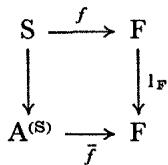
\includegraphics[keepaspectratio]{images/part003_a94682a2.jpg}}

(where the vertical arrow on the left is the canonical mapping \(s \mapsto e_s\) ).

Let \(\bar{f}:\mathbf{A}^{(\mathrm{S})}\to\mathbf{F}\) be the unique A-module homomorphism such that \(\bar{f}(e_{s})=\bar{f}(s)\) (II, §1, no. 11, Corollary 3 to Proposition 17); it suffices to verify that \(\bar{f}\) is an algebra homomorphism and for this it suffices to prove that \(\bar{f}(e_{s}e_{t})=\bar{f}(e_{s})\bar{f}(e_{t})\) , which follows immediately from the definition and the hypothesis \(f(st)=f(s)f(t)\) .

Proposition 6 expresses the fact that the ordered pair consisting of \(\mathbf{A}^{(\mathbb{S})}\) and the canonical mapping \(s\mapsto e_s\) is a solution of the universal mapping problem (Set Theory, IV, §3, no. 1) where \(\Sigma\) is the species of A-algebra structure and the \(\alpha\) -mappings the homomorphisms of S into an A-algebra with only its multiplicative law.

COROLLARY. Let S, S' be two magmas and \(g:S\to S'\) a homomorphism. Then there exists one and only one A-algebra homomorphism \(u:A^{(S)}\to A^{(S')}\) rendering commutative the diagram

\pandocbounded{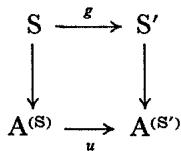
\includegraphics[keepaspectratio]{images/part003_71823134.jpg}}

(where the vertical arrows are the canonical mappings).

It suffices to apply Proposition 6 taking \(f\) to be the composite mapping \(\mathbf{S} \xrightarrow{g} \mathbf{S}' \to \mathbf{A}^{(\mathbf{S}')}\) .

In particular, if T is a stable subset of the magma S (I, § 1, no. 4), the set of elements \(\sum_{s\in\mathbf{T}}\alpha_s e_s\) of \(\mathbf{A}^{(\mathbf{S})}\) is a subalgebra of \(\mathbf{A}^{(\mathbf{S})}\) canonically isomorphic to the algebra \(\mathbf{A}^{(\mathbf{T})}\) and sometimes identified with the latter.

Example. Let V be an A-module and S a monoid which operates on V on the left; this means (I, § 5, no. 1) that there is given a mapping \((s, x) \mapsto s.x\) of S into V such that \(s.(x + y) = s.x + s.y\) , \(s.(\alpha x) = \alpha(s.x)\) and \(s.(t.x) = (st).x\) for \(s, t\) in S, \(x, y\) in V and \(\alpha \in \mathbf{A}\) and, denoting by \(e\) the identity element of S, e.x = x for \(x \in V\) . Writing \(f(s)(x) = s.x\) , f is a homomorphism of S into the algebra \(\operatorname{End}_{\mathbf{A}}(\mathbf{V})\) (with only its multiplicative law), mapping the identity element e to the unit element \(1_{V}\) . Applying Proposition 6, an A-algebra homomorphism \(\bar{f}: \mathbf{A}^{(\mathbf{S})} \to \operatorname{End}_{\mathbf{A}}(\mathbf{V})\) is obtained, which gives the underlying group of V a left module structure over \(\mathbf{A}^{(\mathbf{S})}\) .

This allows us to reduce the study of commutative groups with operators to that of modules. For let M be a commutative group with operators written additively, all of whose external laws are written multiplicatively. Let \(\Omega\) be the sum set (Set Theory, II, §4, no. 8) of the domains of operators of the various external laws on M, each of these domains being canonically identified with a subset of \(\Omega\) . Let \(\mathrm{Mo}(\Omega)\) be the free monoid (I §7, no. 2) constructed on \(\Omega\) ; a law of action

\[
(s, x) \mapsto s. x
\]

is defined on M with \(\mathrm{Mo}(\Omega)\) as domain of operators, by induction on the length of the word s in \(\mathrm{Mo}(\Omega)\) ; if s is of length 0, it is the empty word e and we write e.x = x for all \(x \in M\) . If x is of length \(n \geqslant 1\) , it can be written uniquely as s = tu, where u is of length n - 1 and t of length 1, so that \(t \in \Omega\) ; we then write s.x = t.(u.x). For any two words s, \(s'\) in \(\mathrm{Mo}(\Omega)\) , the relation \(s.(s'.x) = (ss').x\) is verified by induction on the length of s.

Then applying the method described above, a left \(\mathbf{Z}^{(\mathrm{Mo}(\Omega))}\) -module structure is obtained on M and it is verified without difficulty that the usual notions in the theory of groups with operators (stable subgroups, homomorphisms) are the same for commutative groups with operators and the modules thus associated with them.

\subsection{FREE ALGEBRAS}

DEFINITION 2. Let I be a set; let M(I) (resp. Mo(I), resp. N \(^{(I)}\) ) denote the free magma (resp. free monoid, resp. free commutative monoid) derived from I. The algebra of M(I) (resp. Mo(I), resp. N \(^{(I)}\) ) over A is called the free algebra (resp. free associative algebra, resp. free commutative associative algebra (or, by an abuse of language, free commutative algebra)) of the set I over the ring A.

We shall denote the free algebra (resp. free associative algebra, resp. free commutative algebra) of I over A by \(\operatorname{Lib}_{\mathbf{A}}(\mathbf{I})\) (resp. \(\operatorname{Libas}_{\mathbf{A}}(\mathbf{I})\) , resp. \(\operatorname{Libasc}_{\mathbf{A}}(\mathbf{I})\) ). By composing the canonical mapping of I into \(\operatorname{M}(\mathbf{I})\) (resp. \(\operatorname{Mo}(\mathbf{I})\) , resp. \(\mathbf{N}^{(\mathbf{I})}\) ) with the canonical mapping of \(\operatorname{M}(\mathbf{I})\) (resp. \(\operatorname{Mo}(\mathbf{I})\) , resp. \(\mathbf{N}^{(\mathbf{I})}\) ) into \(\operatorname{Lib}_{\mathbf{A}}(\mathbf{I})\) (resp. \(\operatorname{Libas}_{\mathbf{A}}(\mathbf{I})\) , resp. \(\operatorname{Libasc}_{\mathbf{A}}(\mathbf{I})\) ), a canonical mapping is obtained of I into \(\operatorname{Lib}_{\mathbf{A}}(\mathbf{I})\) (resp. \(\operatorname{Libas}_{\mathbf{A}}(\mathbf{I})\) , resp. \(\operatorname{Libasc}_{\mathbf{A}}(\mathbf{I})\) ), which is injective if \(A \neq \{0\}\) . We shall denote the image of an element \(i \in I\) under this canonical mapping by \(X_{i}\) and we shall say that \(X_{i}\) is the indeterminate of index i of \(\operatorname{Lib}_{\mathbf{A}}(\mathbf{I})\) (resp. \(\operatorname{Libas}_{\mathbf{A}}(\mathbf{I})\) , resp. \(\operatorname{Libasc}_{\mathbf{A}}(\mathbf{I})\) ).

As \(\mathbf{Mo}(\mathbf{I})\) and \(\mathbf{N}^{(\mathrm{I})}\) each have an identity element, \(\operatorname{Libas}_{\mathbf{A}}(\mathbf{I})\) and \(\operatorname{Libasc}_{\mathbf{A}}(\mathbf{I})\)

are unital associative algebras and further \(\operatorname{Libasc}_{\mathbf{A}}(\mathbf{I})\) is commutative. If e is the unit element of \(\operatorname{Libas}_{\mathbf{A}}(\mathbf{I})\) (resp. \(\operatorname{Libasc}_{\mathbf{A}}(\mathbf{I})\) ), the mapping \(\alpha \mapsto \alpha e\) is an isomorphism of A onto a subring of the centre of \(\operatorname{Libas}_{\mathbf{A}}(\mathbf{I})\) (resp. \(\operatorname{Libasc}_{\mathbf{A}}(\mathbf{I})\) ), which is identified with A (no. 1).

PROPOSITION 7. Let I be a set and F an algebra (resp. unital associative algebra, resp. unital commutative associative algebra) over A. For every mapping \(f:\mathbf{I}\to\mathbf{F}\) , there exists one and only one homomorphism (resp. unital homomorphism) \(\bar{f}\) of \(\operatorname{Lib}_{\mathbf{A}}(\mathbf{I})\) (resp. \(\operatorname{Libas}_{\mathbf{A}}(\mathbf{I})\) , resp. \(\operatorname{Libasc}_{\mathbf{A}}(\mathbf{I})\) ) into F such that \(\bar{f}(\mathbf{X}_{i})=f(i)\) for all \(i\in\mathbf{I}\) .

Let \(F_{m}\) be the magma (resp. monoid) obtained by giving the set F its multiplicative law of composition. There is one and only one homomorphism (resp. unital homomorphism) g of M(I) (resp. Mo(I), resp. N \(^{(I)}\) ) into \(F_{m}\) such that \(g(i) = f(i)\) for all \(i \in I\) (I, § 7, nos. 1, 2 and 7); Proposition 7 then follows from no. 6, Proposition 6.

Remarks. (1) We shall later define an isomorphism of \(\operatorname{Libas}_{\mathbf{A}}(\mathbf{I})\) onto the tensor algebra of the free module \(\mathbf{A}^{(I)}\) ( \(\S 5\) , no. 5) and also an isomorphism of \(\operatorname{Libasc}_{\mathbf{A}}(\mathbf{I})\) onto the symmetric algebra of \(\mathbf{A}^{(I)}\) ( \(\S 6\) , no. 6).

\begin{enumerate}
\def\labelenumi{(\arabic{enumi})}
\setcounter{enumi}{1}
\item
  Let \(\rho\) be a unital homomorphism of A into a commutative ring B. As has been seen (§ 2, no. 6), an isomorphism \(\sigma\) is derived from \(\rho\) of \(\operatorname{Lib}_{\mathbf{B}}(\mathbf{I})\) (resp. \(\operatorname{Libas}_{\mathbf{B}}(\mathbf{I})\) , resp. \(\operatorname{Libasc}_{\mathbf{B}}(\mathbf{I})\) ) onto the algebra \((\operatorname{Lib}_{\mathbf{A}}(\mathbf{I}))_{(\mathbf{B})}\) (resp. \((\operatorname{Libas}_{\mathbf{A}}(\mathbf{I}))_{(\mathbf{B})}\) , resp. \((\operatorname{Libasc}_{\mathbf{A}}(\mathbf{I}))_{(\mathbf{B})}\) ) obtained by extending the scalars to B by means of \(\rho\) ; if \(\mathbf{X}_i^{\mathbf{A}}\) , \(\mathbf{X}_i^{\mathbf{B}}\) are the indeterminates of index \(i\) corresponding respectively to A and B, then \(\sigma(\mathbf{X}_i^{\mathbf{B}}) = \mathbf{X}_i^{\mathbf{A}} \otimes 1\) .
\item
  Let \(J\) be a subset of \(I\) ; we know that \(M(J)\) is identified with a stable subset of the magma \(M(I)\) and hence (no. 6) \(\operatorname{Lib}_{A}(J)\) is canonically identified with a subalgebra of \(\operatorname{Lib}_{A}(I)\) , generated by the \(X_i\) such that \(i \in J\) ; it is said that only the indeterminates of indices belonging to \(J\) occur in an element of \(\operatorname{Lib}_{A}(J)\) . The definition given in no. 6 of the algebra of a magma shows that \(\operatorname{Lib}_{A}(I)\) is the union of the directed family of subalgebras \(\operatorname{Lib}_{A}(J)\) when \(J\) runs through the set of finite subsets of \(I\) . There are analogous results for \(\operatorname{Libas}_{A}(I)\) and \(\operatorname{Libasc}_{A}(I)\) .
\item
  With element \(s\) of \(\mathbf{M}(\mathbf{I})\) (resp. \(\mathbf{Mo}(\mathbf{I})\) , resp. \(\mathbf{N}^{(1)}\) ) is associated its length \(l(s)\) , which is an integer \(\geqslant 1\) (resp. \(\geqslant 0\) ) such that \(l(ss') = l(s) + l(s')\) (I, §7, nos. 1, 2 and 7). If \(e_s\) is the element of \(\operatorname{Lib}_{\mathbf{A}}(\mathbf{I})\) (resp. \(\operatorname{Libas}_{\mathbf{A}}(\mathbf{I})\) , resp. \(\operatorname{Libasc}_{\mathbf{A}}(\mathbf{I})\) ) corresponding to \(s\) , the total degree (or simply the degree of an element \(x = \sum_{s} \alpha_s e_s \neq 0\) of \(\operatorname{Lib}_{\mathbf{A}}(\mathbf{I})\) (resp. \(\operatorname{Libas}_{\mathbf{A}}(\mathbf{A})\) , resp. \(\operatorname{Libasc}_{\mathbf{A}}(\mathbf{I})\) ) is the greatest of the numbers \(l(s)\) when \(s\) runs through the (non-empty by hypothesis) set of elements such that \(\alpha_s \neq 0\) . For example, if \(i, j, k\) are three distinct elements of \(\mathbf{I}\) , the element \((\mathrm{X}_t(\mathrm{X}_j\mathrm{X}_k))\mathrm{X}_t - (\mathrm{X}_t\mathrm{X}_j)(\mathrm{X}_k\mathrm{X}_l)\) is an element \(\neq 0\) of total degree 4 in \(\operatorname{Lib}_{\mathbf{A}}(\mathbf{I})\) .
\end{enumerate}

\subsection{DEFINITION OF AN ALGEBRA BY GENERATORS AND RELATIONS}

Let \(\mathbf{F}\) be an algebra over \(\mathbf{A}\) and \((x_{i})_{i\in I}\) a family of elements of \(\mathbf{F}\) . By no. 7, Proposition 7, there exists a unique homomorphism \(f\colon \operatorname{Lib}_{\mathbf{A}}(\mathbf{I})\to \mathbf{F}\) such that \(f(\mathbf{X}_i) = x_i\) for all \(i\in I\) . For \(f\) to be surjective, it is necessary and sufficient that \((x_{i})_{i\in I}\) be a generating system of \(\mathbf{F}\) .

If \(\mathbf{U} \in \operatorname{Lib}_{\mathbf{A}}(\mathbf{I})\) , \(f(\mathbf{U})\) is called the element of \(\mathbf{F}\) derived from \(\mathbf{U}\) by substituting the elements \(x_{i}\) for the indeterminates \(\mathbf{X}_{i}\) , or also the value of \(\mathbf{U}\) for the values \(x_{i}\) of the indeterminates \(\mathbf{X}_{i}\) ; it is usually denoted by \(\mathbf{U}((x_{i})_{i \in I})\) ; in particular \(\mathbf{U}((\mathbf{X}_{i})_{i \in I}) = \mathbf{U}\) . If \(\lambda\) is a homomorphism of \(\mathbf{F}\) into an algebra \(\mathbf{F}'\) over \(\mathbf{A}\) , then

\[
\lambda (\mathrm{U} ((x _ {i}) _ {i \in \mathrm{I}})) = \mathrm{U} ((\lambda (x _ {i})) _ {i \in \mathrm{I}}).
\]

Consider in particular the case where \(\mathrm{F} = \operatorname{Lib}_{\mathbf{A}}(\mathbf{J})\) , where J is another set; for every family \((\mathrm{H}_{i})_{i \in I}\) of elements of \(\operatorname{Lib}_{\mathbf{A}}(\mathbf{J})\) and every family \((y_{j}')_{j \in J}\) of elements of an A-algebra \(F'\) ,

\[
\mathrm{U} ((\mathrm{H} _ {i}) _ {i \in I})) ((y _ {j} ^ {\prime}) _ {j \in J}) = \mathrm{U} ((\mathrm{H} _ {i} ((y _ {j} ^ {\prime}) _ {j \in J})) _ {i \in I}).\tag{37}
\]

In the above notation, every element U of \(\operatorname{Lib}_{\mathbf{A}}(\mathbf{I})\) such that \(\mathrm{U}((x_{i})_{i\in\mathbf{I}})=0\) , or also such that \(f(\mathrm{U})=0\) , is called a relator of the family \((x_{i})_{i\in\mathbf{I}}\) in F. The two-sided ideal \(\operatorname{Ker}(f)\) consisting of these elements is called the ideal of relators of \((x_{i})\) .

Let \((\mathbf{R}_j)_{j\in J}\) be a family of elements of \(\operatorname{Lib}_{\mathbf{A}}(\mathbf{I})\) . \(((x_i)_{i\in I}, (\mathbf{R}_j)_{j\in J})\) is called a presentation of the algebra \(F\) if \((x_i)_{i\in I}\) is a generating system of \(F\) and the two-sided ideal of \(\operatorname{Lib}_{\mathbf{A}}(\mathbf{I})\) generated by the \(\mathbf{R}_j\) is equal to the ideal of relators of the family \((x_i)_{i\in I}\) ; the \(x_i\) are called the generators and the \(\mathbf{R}_j\) the relators of the presentation.

Consider now any set I and a family \((\mathbf{R}_j)_{j\in J}\) of elements of \(\operatorname{Lib}_{\mathbf{A}}(\mathbf{I})\) . The quotient algebra E of \(\operatorname{Lib}_{\mathbf{A}}(\mathbf{I})\) by the two-sided ideal generated by the family \((\mathbf{R}_j)\) is called the universal algebra defined by the generating system I related by the family of relators \((\mathbf{R}_j)_{j\in J}\) . Clearly, if \(\overline{\mathbf{X}}_i\) denotes the image of \(\mathbf{X}_i\) in E,

\[
\left(\left(\overline {{\mathbf {X}}} _ {i}\right) _ {i \in I}, \left(\mathbf {R} _ {j}\right) _ {j \in J}\right)
\]

is a presentation of E. Moreover, if \((x_{i})_{i\in I}\) is a family of elements of an algebra F and \(\mathbf{R}_j((x_i)_{i\in I}) = 0\) for all \(j\in J\) , there exists a unique homomorphism \(g:\mathbf{E}\to \mathbf{F}\) such that \(g(\overline{\mathbf{X}}_i) = x_i\) for all \(i\in I\) ; for \(((x_i)_{i\in I},(\mathbf{R}_j)_{j\in J})\) to be a presentation of F, it is necessary and sufficient that \(g\) be bijective.

These remarks justify the following abuse of language: instead of saying `` \(((x_i)_{i \in I}, (R_j)_{j \in J})\) is a presentation of F'', it is also said that ``F is the algebra generated by the generators \(x_i\) subject to the relations \(R_j((x_i)_{i \in I}) = 0\) ''. When the \(R_j\) are of the form \(P_j - Q_j\) , it is also said that ``F is the algebra generated by the \(x_i\) subject to the relations \(P_j((x_i)) = Q_j((x_i))\) ''.

Let H be a set; we shall say that an element S of \(\operatorname{Lib}_{\mathbf{A}}(\mathbf{H})\) is a universal relator for an A-algebra F is \(\mathrm{S}((x_{h})_{h\in\mathbb{H}})=0\) for every family \((x_{h})_{h\in\mathbb{H}}\) of elements of F with H as indexing set.

Examples. (1) Take \(\mathbf{H} = \{1,2,3\}\) ; the algebras which admit

\[
(\mathrm{X} _ {1} \mathrm{X} _ {2}) \mathrm{X} _ {3} - \mathrm{X} _ {1} (\mathrm{X} _ {2} \mathrm{X} _ {3})
\]

as universal relator are the associative algebras. The algebras which admit \(X_{1}X_{2}-X_{2}X_{1}\) as universal relator are the commutative algebras. The algebras which admit the universal relators \(X_{1}X_{1}\) and

\[
(\mathrm{X} _ {1} \mathrm{X} _ {2}) \mathrm{X} _ {3} + (\mathrm{X} _ {2} \mathrm{X} _ {3}) \mathrm{X} _ {1} + (\mathrm{X} _ {3} \mathrm{X} _ {1}) \mathrm{X} _ {2}
\]

as universal relator are the Lie algebras.

Let I be a set; let a family \((\mathrm{S}_{k})_{k\in\mathbb{K}}\) of elements of \(\operatorname{Lib}_{\mathbf{A}}(\mathbf{H})\) be given and consider the set T of elements of \(\operatorname{Lib}_{\mathbf{A}}(\mathbf{I})\) of the form \(\mathrm{S}_{k}((\mathrm{U}_{h}))_{h\in\mathbb{H}}\) , where k runs through K and, for each \(k,\left(\mathrm{U}_{h}\right)_{h\in\mathbb{H}}\) runs through the set of families of elements of \(\operatorname{Lib}_{\mathbf{A}}(\mathbf{I})\) with H as indexing set; consider a family \((\mathrm{R}_{j})_{j\in\mathbb{J}}\) with T as set of elements. Then let F be the universal algebra defined by the generating system I related by the family \((\mathrm{R}_{j})_{j\in\mathbb{J}}\) and let \(u:\operatorname{Lib}_{\mathbf{A}}(\mathbf{I})\to\mathbf{F}\) be the canonical homomorphism, so that \(\operatorname{Ker}(u)\) is generated by the elements \(\mathrm{S}_{k}((\mathrm{U}_{h})_{h\in\mathbb{H}})\) for all \(k\in K\) and all families \((\mathrm{U}_{h})_{h\in\mathbb{H}}\) of elements of \(\operatorname{Lib}_{\mathbf{A}}(\mathbf{I})\) ; clearly each of the \(S_{k}\) \((k\in\mathbb{K})\) is a universal relator for F. Now let \(F'\) be an algebra admitting a generating system \((x_{i})_{i\in\mathbb{I}}\) , for which each of the \(S_{k}\) is a universal relator, and let \(u':\operatorname{Lib}_{\mathbf{A}}(\mathbf{I})\to\mathbf{F}'\) be the homomorphism such that \(u'(\mathrm{X}_{i})=x_{i}\) for all \(i\in I\) ; clearly \(\operatorname{Ker}(u)\subset\operatorname{Ker}(u')\) and hence \(u'\) can be written uniquely in the form \(u'=h\circ u\) , where \(h:F\to F'\) is a homomorphism such that \(h(\overline{\mathrm{X}}_{i})=x_{i}\) for all \(i\in I\) . For this reason F is called the universal algebra defined by the generating system I, corresponding to the family of universal relators \((\mathrm{S}_{k})_{k\in\mathbb{K}}\) . By an abuse of language, F is sometimes called the universal algebra generated by I and subject to the identities \(\mathrm{S}_{k}((u_{h}))=0\) for every family \((u_{h})_{h\in\mathbb{H}}\) of elements of F.

Example 2. Let \(\mathbf{L}'\) be the universal algebra generated by \(\mathbf{I}\) and subject to the identities \((uv)w - u(vw) = 0\) for every family of three elements of \(\mathbf{L}'\) and let \(\mathbf{L}''\) be the algebra obtained by adjoining a unit element to \(\mathbf{L}'\) ; then there exists a unique unital isomorphism \(g\) of \(\mathbf{L}''\) onto \(\operatorname{Libas}_{\mathbf{A}}(\mathbf{I})\) such that \(g(\overline{\mathbf{X}}_i) = \mathbf{X}_i\) for all \(i \in \mathbf{I}\) . For clearly \(\mathbf{L}''\) is associative and the existence of the homomorphism \(g\) follows from the definition of \(\mathbf{L}'\) and the remarks preceding it; but then clearly \(\mathbf{L}''\) satisfies the universal property (no. 7, Proposition 7) which characterizes \(\operatorname{Libas}_{\mathbf{A}}(\mathbf{I})\) , whence the conclusion.

Considerations analogous to the above can be applied to associative algebras (resp. commutative associative algebras), taking account of the following remarks. When the context gives sufficient indication that the algebras considered are unital algebras, by an abuse of language, a family of elements \((x_{i})_{i\in I}\) of an algebra \(F\) , such that the subalgebra generated by the \(x_{i}\) ( \(i\in I\) ) and the unit element is equal to \(F\) , is often called a generating system of \(F\) . Then let \(F\) be a unital associative algebra over \(A\) and let \((x_{i})_{i\in I}\) be a family of elements of \(F\) ; by virtue of no. 7, Proposition 7, there exists a unique unital homomorphism \(f:\mathrm{Libas}_{\mathbf{A}}(\mathbf{I})\to F\) such that \(f(\mathbf{X}_i) = x_i\) for all \(i\in I\) ; if \(\mathbf{U}\in \mathrm{Libas}_{\mathbf{A}}(\mathbf{I}), f(\mathbf{U})\) is also called the element of \(F\) derived from \(\mathbf{U}\) by substituting the elements \(x_{i}\) for the indeterminates \(\mathbf{X}_i\) and it is also denoted by \(\mathrm{U}((x_{i})_{i\in I})\) . Then the notions of relator, presentation and universal relator go over immediately to associative algebras; it suffices simply to replace \(\mathrm{Lib}_{\mathbf{A}}(\mathbf{I})\) throughout by \(\mathrm{Libas}_{\mathbf{A}}(\mathbf{I})\) . The universal unital associative algebra defined by the generating system \(I\) related by the family of relators \((\mathbb{R}_j)_{j\in J}\) is the quotient algebra of \(\mathrm{Libas}_{\mathbf{A}}(\mathbf{I})\) by the two-sided ideal generated by the family \((\mathbb{R}_j)\) . The universal unital associative algebra generated by the generating system \(I\) , corresponding to a family of universal relators is defined similarly. We leave to the reader the task of stating the analogous definitions relative to commutative associative algebras with \(\mathrm{Libasc}_{\mathbf{A}}(\mathbf{I})\) substituted for \(\mathrm{Libas}_{\mathbf{A}}(\mathbf{I})\) .

Example 3. Let L' be the universal unital associative algebra generated by I and subject to the identities uv - vu = 0 for every family of two elements of L'. It is seen, as in Example 2, that L' is canonically isomorphic to \(\text{Libasc}_{\mathbf{A}}(\mathbf{I})\) .

\subsection{POLYNOMIAL ALGEBRAS}

Let B be a unital commutative associative A-algebra and let \((x_{i})_{i\in I}\) be a family of elements of B; the subalgebra of B generated by the \(x_{i}\) ( \(i\in I\) ) and the unit element is denoted by \(\mathrm{A}[(x_{i})_{i\in I}]_{\mathrm{B}}\) or simply \(\mathrm{A}[(x_{i})_{i\in I}]\) when no confusion can arise. For every set I, the algebra \(\operatorname{Libasc}_{\mathbf{A}}(\mathbf{I})\) is therefore equal to \(\mathrm{A}[(\mathbf{X}_{i})_{i\in I}]\) (also denoted by \(\mathrm{A}[\mathbf{X}_{i}]_{i\in I}\) ); the latter notation, which has the advantage of indicating the notation chosen to denote the indeterminates, is the one we shall generally use in the rest of this Treatise. The elements of \(\mathrm{A}[(\mathbf{X}_{i})_{i\in I}]\) are called polynomials in the indeterminates \(X_{i}\) ( \(i\in I\) ) with coefficients in A; it is a convention that, when it is said ``let \(\mathrm{A}[(\mathbf{X}_{i})_{i\in I}]\) be a polynomial algebra'', the \(X_{i}\) are always understood to be the indeterminates. For every subset J of I, the use of the above notation amounts to identifying \(\operatorname{Libasc}_{\mathbf{A}}(\mathbf{J})\) with the algebra of \(\operatorname{Libasc}_{\mathbf{A}}(\mathbf{I})\) generated by the \(X_{i}\) of index \(i\in J\) and the unit element (cf.~no. 7, Remark (3)). For \(I=\{1,2,\ldots,n\}\) , we write \(\mathrm{A}[\mathbf{X}_{1},\mathbf{X}_{2},\ldots,\mathbf{X}_{n}]\) instead of \(\mathrm{A}[(\mathbf{X}_{i})_{i\in I}]\) .

If I and I' are two equipotent sets, the algebras \(\operatorname{Libasc}_{\mathbf{A}}(\mathbf{I})\) and \(\operatorname{Libasc}_{\mathbf{A}}(\mathbf{I}')\) are isomorphic. A{[}X{]} is often used to denote the polynomial algebra corresponding to an unspecified indexing set with a single element, X denoting the unique indeterminate; similarly, A{[}X, Y{]}, A{[}X, Y, Z{]}, \ldots{} are used to denote the polynomial algebras corresponding to unspecified indexing sets with

2, 3, \ldots{} elements. Note that, by virtue of the conventions made above, A{[}X{]} and A{[}Y{]} are for example (distinct) subalgebras of A{[}X, Y, Z{]} if A ≠ \{0\}.

The elements

\[
\mathrm{X} ^ {\nu} = \prod_ {i \in I} \mathrm{X} _ {i} ^ {\nu (i)},
\]

where v runs through \(\mathbf{N}^{(1)}\) form a basis of the polynomial algebra \(\mathrm{A}[(\mathrm{X}_{i})_{i\in\mathbb{I}}]\) . These elements are called monomials in the indeterminates \(X_{i}\) and the number \(|v|=\sum_{i\in\mathbb{I}}v(i)\) is called the degree (or total degree) of the monomial \(X^{v}\) . The unique monomial of degree 0 is the unit element of \(\mathrm{A}[(\mathrm{X}_{i})_{i\in\mathbb{I}}]\) ; it is often identified with the unit element 1 of A. Every polynomial u of \(\mathrm{A}[(\mathrm{X}_{i})_{i\in\mathbb{I}}]\) can be written uniquely as

\[
u = \sum_ {v \in \mathbf {N} ^ {(I)}} \alpha_ {v} X ^ {v}
\]

with \(\alpha_{\nu} \in \mathbf{A}\) ; the elements \(\alpha_{\nu}\) , zero except for a finite number of indices \(\nu \in \mathbf{N}^{(1)}\) , are called the coefficients of \(u\) ; the elements \(\alpha_{\nu} \mathrm{X}^{\nu}\) are called the terms of \(u\) (the element \(\alpha_{\nu} \mathrm{X}^{\nu}\) often being called the ``term in \(\mathrm{X}^{\nu''}\) ); in particular the term \(\alpha_{0} \mathrm{X}^{0}\) (identified with \(\alpha_{0} \in \mathbf{A}\) ) is called the constant term of \(u\) . If \(J\) is a subset of \(I\) , \(u\) belongs to \(\mathrm{A}[(\mathrm{X}_{i})_{i \in J}]\) if and only if \(\alpha_{\nu} = 0\) for \(\nu \notin \mathbf{N}^{(J)}\) . It follows that \(\mathrm{A}[(\mathrm{X}_{i})_{i \in I}]\) is the union of the subalgebras \(\mathrm{A}[(\mathrm{X}_{i})_{i \in J}]\) , where \(J\) runs through the set of finite subsets of \(I\) . If \(\alpha_{\nu} = 0\) for \(|\nu| > n\) , \(u\) is said to be a polynomial of degree \(\leqslant n\) . When \(\alpha_{\nu} = 0\) , (by an abuse of language) \(u\) is said to contain no term in \(\mathrm{X}^{\nu'}\) ; in particular, when \(\alpha_{0} = 0\) , \(u\) is said to be a polynomial with no constant term.

For every non-zero polynomial \(u = \sum_{v} \alpha_v X^v\) , the degree (or total degree) of \(u\) is the greatest of the integers \(|v|\) of the multiindices \(v\) such that \(\alpha_v \neq 0\) .

Let F be a unital associative A-algebra and let \((x_{i})_{i\in I}\) be a family of elements of F, which are pairwise permutable. The subalgebra \(F'\) of F generated by the \(x_{i}\) and the unit element is commutative (§1, no. 7), which allows us to define substituting the \(x_{i}\) for the \(X_{i}\) in the polynomial \(u\in\mathrm{A}[(X_{i})_{i\in I}]\) (although F is not necessarily commutative): \(u((x_{i})_{i\in I})\) is an element of \(F'\) and therefore of F and \(h\colon u\to u((x_{i})_{i\in I})\) is a homomorphism of \(\mathrm{A}[(X_{i})_{i\in I}]\) into F. The elements of the kernel of h are the relators of the family \((x_{i})\) in \(\mathrm{A}[(X_{i})_{i\in I}]\) , also called polynomial relators (with coefficients in A) between the \(x_{i}\) . The image of the homomorphism h is the subalgebra \(F'\) , also denoted by \(\mathrm{A}[(x_{i})_{i\in I}]\) (even when F is not commutative); if a is the ideal of polynomial relators between the \(x_{i}\) , then there is an exact sequence of A-modules

\[
0 \longrightarrow a \longrightarrow A [ (X _ {i}) _ {i \in I} ] \stackrel {h} {\longrightarrow} A [ (x _ {i}) _ {i \in I} ] \longrightarrow 0.
\]

PROPOSITION 8. Let \(\mathbf{A}[(\mathbf{X}_i)_{i\in I}]\) be a polynomial algebra, \(J\) a subset of \(I\) and \(K\) the complement of \(J\) in \(I\) . Writing \(\mathbf{A}' = \mathbf{A}[(\mathbf{X}_j)_{j\in J}]\) and denoting by \(\mathbf{X}_k'\) ( \(k\in K\) ) the indeterminates in the polynomial algebra \(\operatorname{Libasc}_{\mathbf{A}'}(\mathbf{K}) = \mathbf{A}'[(\mathbf{X}_k')_{k \in \mathbb{K}}]\) , there exists a unique ring isomorphism of \(\mathbf{A}'[(\mathbf{X}_k')_{k \in \mathbb{K}}]\) onto \(\mathbf{A}[(\mathbf{X}_i)_{i \in I}]\) which coincides with the identity on \(\mathbf{A}'\) and maps \(\mathbf{X}_k'\) to \(\mathbf{X}_k\) for all \(k \in \mathbb{K}\) .

Clearly \(\mathbf{A}[(\mathbf{X}_i)_{i\in I}]\) is an \(\mathbf{A}'\) -algebra generated by the \(\mathbf{X}_k\) for \(k\in \mathbf{K}\) . On the other hand, as a polynomial relator between the \(\mathbf{X}_k\) ( \(k\in \mathbf{K}\) ) with coefficients in \(\mathbf{A}'\) can be written uniquely as \(\sum_{\nu}h_{\nu}((\mathbf{X}_j)_{j\in J})\mathbf{X}^{\nu}\) where \(\nu\) runs through a finite subset of \(\mathbf{N}^{(\mathbb{R})}\) and where the \(h_\nu\) are elements of \(\mathbf{A}[(\mathbf{X}_j)_{j\in J}]\) , the \(h_\nu\) must be polynomial relators between the \(\mathbf{X}_j\) with coefficients in \(\mathbf{A}\) and hence are all zero, which proves the proposition.

The isomorphism described in Proposition 8 is often used to identify the elements of \(\mathbf{A}[(\mathbf{X}_i)_{i\in I}]\) with polynomials with coefficients in \(\mathbf{A}' = \mathbf{A}[(\mathbf{X}_j)_{j\in J}]\) . If \(u\) is an element \(\neq 0\) of \(\mathbf{A}[(\mathbf{X}_i)_{i\in I}]\) , its total degree considered as an element of \(\mathbf{A}'[(\mathbf{X}_k)_{k\in K}]\) is also called its degree with respect to the \(\mathbf{X}_i\) of index \(i\in K\) .

Remark. Let I and J be two sets and \((\mathrm{P}_{j})_{j\in J}\) a family of elements of \(\mathbf{Z}[(\mathrm{X}_{i})_{i\in I}]\) ; if Q is an element of \(\mathbf{Z}[(\mathrm{X}_{j})_{j\in J}]\) such that \(\mathbf{Q}((\mathrm{P}_{j})_{j\in J})=0\) , then, for every family \((b_{i})_{i\in I}\) of pairwise permutable elements of a ring B,

\[
\mathrm{Q} ((\mathrm{P} _ {j} ((b _ {i}) _ {i \in \mathrm{I}})) _ {j \in \mathrm{J}}) = 0.
\]

The relations which hold of the form \(\mathbf{Q}((\mathbf{P}_{j})_{j\in\mathbf{J}})=0\) are sometimes called polynomial identities. For example

\[
\left(\mathrm{X} _ {1} + \mathrm{X} _ {2}\right) ^ {2} - \mathrm{X} _ {1} ^ {2} - \mathrm{X} _ {2} ^ {2} - 2 \mathrm{X} _ {1} \mathrm{X} _ {2} = 0
\]

with

\[
\begin{array}{r l} \mathrm{Q} & = \mathrm{Y} _ {1} ^ {2} - \mathrm{Y} _ {2}, \qquad \mathrm{P} _ {1} = \mathrm{X} _ {1} + \mathrm{X} _ {2}, \qquad \mathrm{P} _ {2} = \mathrm{X} _ {1} ^ {2} + \mathrm{X} _ {2} ^ {2} + 2 \mathrm{X} _ {1} \mathrm{X} _ {2} \\ & \quad \mathrm{X} _ {1} ^ {n} - \mathrm{X} _ {2} ^ {n} - (\mathrm{X} _ {1} - \mathrm{X} _ {2}) (\mathrm{X} _ {1} ^ {n - 1} + \mathrm{X} _ {1} ^ {n - 2} \mathrm{X} _ {2} + \dots + \mathrm{X} _ {2} ^ {n - 1}) = 0 \end{array}
\]

with

\[
\begin{array}{c} \mathrm{Q} = \mathrm{Y} _ {1} - \mathrm{Y} _ {2} \mathrm{Y} _ {3}, \qquad \mathrm{P} _ {1} = \mathrm{X} _ {1} ^ {n} - \mathrm{X} _ {2} ^ {n}, \qquad \mathrm{P} _ {2} = \mathrm{X} _ {1} - \mathrm{X} _ {2}, \\ \mathrm{P} _ {3} = \mathrm{X} _ {1} ^ {n - 1} + \mathrm{X} _ {1} ^ {n - 2} \mathrm{X} _ {2} + \dots + \mathrm{X} _ {2} ^ {n - 1} \end{array}
\]

are polynomial identities.

\subsection{TOTAL ALGEBRA OF A MONOID}

The algebra of a monoid S over A is (as an A-module) the submodule of the product \(A^{s}\) consisting of the families \((\alpha_{s})_{s\in\mathbb{S}}\) of finite support; the multiplication in this algebra is defined by the relations \((\alpha_{s})(\beta_{s})=(\gamma_{s})\) , where, for all \(s\in S\) ,

\[
\gamma_ {s} = \sum_ {t u = s} \alpha_ {t} \beta_ {u}\tag{38}
\]

(cf.~no. 6, formula (35)). The sum on the right hand side of (38) is meaningful because \((\alpha_{s})\) and \((\beta_{s})\) are families of finite support and so therefore is the double family \((\alpha_{t}\beta_{u})_{(t,u)\in S\times S}\) . But the right hand side of (38) is also meaningful for arbitrary elements \((\alpha_{s})\) , \(\beta_{s})\) of \(A^{S}\) when the monoid \(S\) satisfies the following condition:

\begin{enumerate}
\def\labelenumi{(\Alph{enumi})}
\setcounter{enumi}{3}
\tightlist
\item
  For all \(s \in \mathbf{S}\) , there exists only a finite number of ordered pairs \((t, u)\) in \(\mathbf{S} \times \mathbf{S}\) such that \(tu = s\) .
\end{enumerate}

Suppose then that S satisfies condition (D); a multiplication law can then be defined on the product A-module \(A^{s}\) by formula (38). It is immediate that the multiplication thus defined on \(A^{s}\) is A-bilinear; also it is associative, since, for \(\alpha\) , \(\beta\) , \(\gamma\) in \(A^{s}\) ,

\[
\sum_ {u v w = t} \alpha_ {u} \beta_ {v} \gamma_ {w} = \sum_ {r w = t} \left(\left(\sum_ {u v = r} \alpha_ {u} \beta_ {v}\right) \gamma_ {w}\right) = \sum_ {u s = t} \left(\alpha_ {u} \left(\sum_ {v w = s} \beta_ {v} \gamma_ {w}\right)\right).
\]

This multiplication and the A-module structure on \(A^{s}\) therefore define on \(A^{s}\) a unital associative algebra structure over A; we shall say that the set \(A^{s}\) , with this structure, is the total algebra of the monoid S over A.

It is immediate that the algebra \(\mathbf{A}^{(\mathbf{S})}\) of the monoid \(\mathbf{S}\) over \(\mathbf{A}\) (also called the restricted algebra of \(\mathbf{S}\) when necessary to avoid confusion) is a subalgebra of the total algebra of \(\mathbf{S}\) over \(\mathbf{A}\) (and is identical with the latter when \(\mathbf{S}\) is finite). By an abuse of language, every element \((\xi_s)_{s \in \mathbf{S}}\) of the total algebra of \(\mathbf{S}\) over \(\mathbf{A}\) is also denoted by the same notation \(\sum_{s \in \mathbf{S}} \xi_s e_s\) (or even \(\sum_{s \in \mathbf{S}} \xi_s s\) ) as the elements of the restricted algebra of \(\mathbf{S}\) ; of course the summation symbol appearing in this notation corresponds to no algebraic operation because it is taken over an infinity of terms \(\neq 0\) in general. With this notation, multiplication in the total algebra of \(\mathbf{S}\) is also given by formula (35) of no. 6.

If S is commutative, so is its total algebra \(A^{S}\) . If T is a submonoid of S, the total algebra \(A^{T}\) of the monoid is canonically identified with a subalgebra of the total algebra of S. If \(\rho: A \to B\) is a ring homomorphism, the canonical extension \(\rho^{S}: A^{S} \to B^{S}\) is an A-homomorphism of the total algebra of S over A into the total algebra of S over B, which extends the canonical homomorphism \(A^{(S)} \to B^{(S)}\) .

\subsection{FORMAL POWER SERIES OVER A COMMUTATIVE RING}

For every set I, the additive monoid \(\mathbf{N}^{(I)}\) satisfies condition (D) of no. 10; for, if \(s = (n_i)_{i \in I}\) with \(n_i = 0\) except for the indices \(i\) in a finite subset \(\mathbf{H}\) of I, the relation \(s = t + u\) with \(t = (p_i)_{i \in I}\) and \(u = (q_i)_{i \in I}\) is equivalent to \(p_i + q_i = n_i\) for all \(i\) ; but this implies \(p_i = q_i = 0\) for \(i \notin \mathbf{H}\) and \(p_i \leqslant n_i\) , \(q_i \leqslant n_i\) for \(i \in \mathbf{H}\) ; there are therefore \(\prod_{i \in \mathbf{H}} (n_i + 1)\) ordered pairs \((t, u)\) in \(\mathbf{N}^{(I)}\) such that \(t + u = s\) .

We can therefore consider the total algebra of the monoid \(\mathbf{N}^{(I)}\) over A, which contains the (restricted) algebra \(\mathrm{A}[\mathbf{X}_i]_{i\in I}\) of this monoid. It is a unital commutative associative algebra called the algebra of formal power series in the indeterminates \(\mathbf{X}_i\) ( \(i\in I\) ) with coefficients in A and denoted by \(\mathrm{A}[[\mathbf{X}_i]]_{i\in I}\) ; its elements are called formal power series in the indeterminates \(\mathbf{X}_i\) ( \(i\in I\) ) with coefficients in A. Such an element \((\alpha_{\nu})_{\nu \in \mathbf{N}^{(I)}}\) is also denoted, following the convention made in no. 10, by \(\sum_{\nu \in \mathbf{N}^{(I)}}\alpha_{\nu}\mathbf{X}^{\nu}\) ; the \(\alpha_{\nu}\) are the coefficients of the formal power series and the \(\alpha_{\nu}\mathbf{X}^{\nu}\) its terms; a polynomial in the \(\mathbf{X}_i\) is therefore a formal power series with only a finite number of terms \(\neq 0\) .

Clearly an algebra isomorphism \(\mathbf{A}[[\mathbf{X}_i]]_{i\in I_1}\to \mathbf{A}[[\mathbf{X}_i]]_{i\in I_2}\) is canonically derived from every bijection \(\sigma \colon I_1\to I_2\) by mapping the formal power series \(\sum_{(n_i)}\alpha_{(n_i)}\cdot \prod_{i\in I_1}\mathbf{X}_i^{n_i}\) to the formal power series \(\sum_{(n_i)}\alpha_{(n_i)}\cdot \prod_{i\in I_1}\mathbf{X}_{\sigma (i)}^{n_i}\) .

Let \(J\) be a subset of \(I\) ; the algebra \(A[[X_i]]_{i \in J}\) can be identified with a subalgebra of \(A[[X_i]]_{i \in I}\) consisting of the formal power series \(\sum_{(n_i)} \alpha_{(n_i)} \cdot \prod_{i \in I} X_i^{n_i}\) where \(\alpha_{(n_i)} = 0\) for every element \((n_i) \in \mathbf{N}^{(I)}\) such that \(n_i \neq 0\) for at least one index \(i \in I - J\) . Further, if \(K = I - J\) , \(A[[X_i]]_{i \in I}\) is canonically identified with \((A[[X_j]]_{j \in J})[[X_k]]_{k \in K}\) , by identifying the formal power series \(\sum_{(n_i)} \alpha_{(n_i)} \cdot \prod_{i \in I} X_i^{n_i}\) with the formal power series \(\sum_{(m_k)} \beta_{(m_k)} \cdot \prod_{k \in K} X_k^{m_k}\) , where

\[
\beta_ {(m _ {k})} = \sum_ {(p _ {j})} \gamma_ {(p _ {j})} \cdot \prod_ {j \in J} X _ {j} ^ {p _ {j}}
\]

with \(\gamma_{(p_i)} = \alpha_{(n_i)}\) for the sequence \((n_i)\) such that \(n_i = p_i\) for \(i \in \mathbf{J}\) and \(n_i = m_i\) for \(i \in \mathbf{K}\) .

Given a formal power series \(u = \sum_{\nu} \alpha_{\nu} X^{\nu}\) , the terms \(\alpha_{\nu} X^{\nu}\) such that \(|\nu| = p\) are called the terms in \(u\) of total degree \(p\) . The formal power series \(u_p\) whose terms of total degree \(p\) are those of \(u\) and whose other terms are zero, is called the homogenous part of \(u\) of degree \(p\) ; when I is finite, \(u_p\) is a polynomial for all \(p\) ; \(u_0\) is identified with an element of A (also called the constant term of \(u\) ). If \(u\) and \(v\) are two formal power series and \(w = uv\) , then

\[
w _ {p} = \sum_ {r = 0} ^ {p} u _ {r} v _ {p - r}\tag{39}
\]

for every integer \(p \geqslant 0\) .

For every formal power series \(u \neq 0\) , the least integer \(p \geqslant 0\) such that \(u_{p} \neq 0\) is called the total order (or simply the order) of u. If this order is denoted by \(\omega(u)\) and u and v are two formal power series \(\neq 0\) , then

\[
\omega (u + v) \geqslant \inf (\omega (u), \omega (v)) \quad \text { if } u + v \neq 0\tag{40}
\]

\[
\omega (u v) \geqslant \omega (u) + \omega (v) \quad \text { if } u v \neq 0.\tag{41}
\]

Further, if \(\omega(u) \neq \omega(v)\) , then necessarily \(u + v \neq 0\) and the two sides of (40) are equal.

Note that the order of 0 is not defined. By an abuse of language, it is a convention to say that ``f is a formal power series of order \(\geqslant p\) (resp. \textgreater p)'' if the homogeneous part of f of degree n is zero for all n \textless{} p (resp. \(n \leqslant p\) ); 0 is therefore a ``formal power series of order \textgreater p'' for every integer \(p \geqslant 0\) .

Let \(J\) be a subset of \(I\) and let \(A[[X_i]]_{i \in I}\) be identified as above with \(B[[X_k]]_{k \in K}\) , where \(K = I - J\) and \(B = A[[X_j]]_{j \in J}\) ; corresponding to the above definitions applied to \(B[[X_k]]_{k \in K}\) there are new definitions for the formal power series \(u \in A[[X_i]]_{i \in I}\) ; a term \(\alpha_{(n_i)} \cdot \prod_{i \in I} X_i^{n_i}\) is said to be of degree \(p\) in the \(X_i\) of index \(i \in K\) if \(\sum_{i \in K} n_i = p\) and the formal power series of \(B[[X_k]]_{k \in K}\) with the same terms of degree \(p\) as \(u\) and the others zero is called the homogenous part of degree \(p\) in the \(X_i\) of index \(i \in K\) . If \(u \neq 0\) , the order \(\omega_K(u)\) with respect to the \(X_i\) of index \(i \in K\) is the smallest of the integers \(p \geqslant 0\) such that the homogeneous part of \(u\) of degree \(p\) in the \(X_i\) of index \(i \in K\) is \(\neq 0\) . Inequalities (40) and (41) still hold when \(\omega\) is replaced by \(\omega_K\) .

\section{GRADED ALGEBRAS}

The graduations considered in this paragraph will have as set of degrees a commutative monoid written additively whose identity element is denoted by 0.

\subsection{GRADED ALGEBRAS}

DEFINITION 1. Let \(\Delta\) be a commutative monoid, A a graded ring of type \(\Delta\) (II, § 11, no. 2), \((\mathbf{A}_{\lambda})_{\lambda \in \Delta}\) its graduation and E an A-algebra. A graduation \((\mathbf{E}_{\lambda})_{\lambda \in \Delta}\) of type \(\Delta\) on the additive group E is said to be compatible with the A-algebra structure on E if it is compatible both with the A-module and with the ring structure on E, in other words, if, for all \(\lambda, \mu\) in \(\Delta\) ,

\[
\mathrm{A} _ {\lambda} \mathrm{E} _ {\mu} \subset \mathrm{E} _ {\lambda + \mu}\tag{1}
\]

\[
\mathbf {E} _ {\lambda} \mathbf {E} _ {\mu} \subset \mathbf {E} _ {\lambda + \mu}\tag{2}
\]

The A-algebra E, with this graduation, is then called a graded algebra of type \(\Delta\) over the graded ring A.

When the graduation on A is trivial (that is (II, § 11, no. 1) \(\mathbf{A}_0 = \mathbf{A}, \mathbf{A}_{\lambda} = \{0\}\) for \(\lambda \neq 0\) ), condition (1) means that the \(\mathbf{E}_{\lambda}\) are sub-A-modules of E. This leads to the definition of the notion of graded algebra of type \(\Delta\) over a non-graded commutative ring A: A is given the trivial graduation of type \(\Delta\) and the above definition is applied.

When we consider graded A-algebras E with a unit element \(e\) , it will always be understood that \(e\) is of degree 0 (cf.~Exercise 1).

It follows that if an invertible element \(x \in E\) is homogeneous and of degree p, its inverse \(x^{-1}\) is homogeneous and of degree -p: it suffices to decompose \(x^{-1}\) as a sum of homogeneous elements in the relations \(x^{-1}x = xx^{-1} = e\) .

Let E and \(E'\) be two graded algebras of type \(\Delta\) over a graded ring A of type \(\Delta\) . An A-algebra homomorphism \(u: E \to E'\) is called a graded algebra homomorphism if \(u(E_{\lambda}) \subset E_{\lambda}'\) for all \(\lambda \in \Delta\) (where \((E_{\lambda})\) and \((E_{\lambda}')\) denote the respective graduations of E and \(E')\) ; where E and \(E'\) are associative and unital and u is unital, this condition means that u is a graded ring homomorphism (II, §11, no. 2).

Let E be a graded A-algebra of type N. E is identified with a graded A-algebra of type Z by writing \(E_{n} = \{0\}\) for n \textless{} 0.

Remark. Definition 1 can also be interpreted by saying that E is a graded A-module and that the A-linear mapping

\[
m \colon \mathbf {E} \otimes_ {\mathbf {A}} \mathbf {E} \rightarrow \mathbf {E}
\]

defining the multiplication on E (§ 1, no. 3), is homogeneous of degree 0 when E ⊗\_A E is given its graduation of type Δ (II, § 11, no. 5).

To define a graded A-algebra structure of type \(\Delta\) on the graded ring A, with E as underlying graded A-module, therefore amounts to defining for each ordered pair \((\lambda, \mu)\) of elements of \(\Delta\) a Z-bilinear mapping

\[
m _ {\lambda \mu}: \mathrm{E} _ {\lambda} \times \mathrm{E} _ {\mu} \rightarrow \mathrm{E} _ {\lambda + \mu}
\]

such that for every triple of indices \((\lambda, \mu, \nu)\) and for \(\alpha \in \mathbf{A}_{\lambda}\) , \(x \in \mathbf{E}_{\mu}\) , \(y \in \mathbf{E}_{\nu}\) , \(\alpha \cdot m_{\mu\nu}(x, y) = m_{\lambda + \mu, \nu}(\alpha x, y) = m_{\mu, \lambda + \nu}(x, \alpha y)\) .

Examples. (1) Let B be a graded ring of type \(\Delta\) ; if B is given its canonical \(\mathbf{Z}\) -algebra structure ( \(\S 1\) , no. 1, Example 2), B is a graded A-algebra ( \(\mathbf{Z}\) being given the trivial graduation).

\begin{enumerate}
\def\labelenumi{(\arabic{enumi})}
\setcounter{enumi}{1}
\item
  Let \(\mathbf{A}\) be a graded commutative ring of type \(\Delta\) and \(\mathbf{M}\) a graded A-module of type \(\Delta\) . Suppose that all the elements of the monoid \(\Delta\) are cancellable, which allows (II, § 11, no. 6) us to define on \(\operatorname{Homgr}_{\mathbf{A}}(\mathbf{M}, \mathbf{M}) = \operatorname{Endgr}_{\mathbf{A}}(\mathbf{M})\) a graded A-module structure of type \(\Delta\) ; as this graduation is compatible with the ring structure on \(\operatorname{Endgr}_{\mathbf{A}}(\mathbf{M})\) (II, § 11, no. 6), it defines a unital graded A-algebra structure on the A-algebra \(\operatorname{Endgr}_{\mathbf{A}}(\mathbf{M})\) .
\item
  Algebra of a magma. Let S be a magma and \(\phi: S \to \Delta\) a homomorphism. For all \(\lambda \in \Delta\) , we write \(S_{\lambda} = \phi^{-1}(\lambda)\) ; then \(S_{\lambda}S_{\mu} \subset S_{\lambda + \mu}\) . Let A be a graded commutative ring of type \(\Delta\) and \((A_{\lambda})_{\lambda \in \Delta}\) its graduation; we shall define a graded A-algebra structure on the algebra \(E = A^{(S)}\) of the magma S (§ 2, no. 6). To this end, let \(\mathbf{E}_{\lambda}\) denote the additive subgroup of \(\mathbf{E}\) generated by the elements of the form \(\alpha .s\) such that \(\alpha \in \mathbf{A}_{\mu}, s \in \mathrm{S}_{\nu}\) and \(\mu + \nu = \lambda\) . As the \(\mathrm{S}_{\lambda}\) are pairwise disjoint, \(\mathbf{E}\) is the direct sum of the \(\mathbf{A}_{\mu}\mathrm{S}_{\nu}\) and hence also the direct sum of the \(\mathbf{E}_{\lambda}\) and it is immediate that the \(\mathbf{E}_{\lambda}\) satisfy conditions (1) and (2) and therefore define on \(\mathbf{E}\) the desired graded A-algebra structure. If \(\mathbf{S}\) admits an identity element \(e\) , it may also be supposed that \(\phi(e) = 0\) . A particular case is the one where the graduation of the ring \(\mathbf{A}\) is trivial; then \(\mathbf{E}_{\lambda}\) is the sub-A-module of \(\mathbf{E}\) generated by \(\mathrm{S}_{\lambda}\) . More particularly, if we take \(\mathbf{S} = \mathbf{N}^{(I)}, \Delta = \mathbf{N}\) and \(\phi\) the mapping such that \(\phi((n_{i})) = \sum_{i \in I} n_{i}\) , the ring \(\mathbf{A}\) having the trivial graduation, a graduation is thus obtained on the polynomial algebra \(\mathbf{A}[\mathbf{X}_{i}]_{i \in I}\) , for which the degree of a homogeneous polynomial \(\neq 0\) is the total degree defined in §2, no. 9 (cf.~§6, no. 6).
\end{enumerate}

We now take S to be the free monoid Mo(B) of a set B (I, § 7, no. 2) and \(\phi\) the homomorphism \(\mathrm{Mo(B)} \to \mathbf{N}\) which associates with each word its length. Thus a graded A-algebra structure is obtained on the free associative algebra of the set B (§ 2, no. 7; cf.~§ 5, no. 5).

\subsection{GRADED SUBALGEBRAS, GRADED IDEALS OF A GRADED ALGEBRA}

Let E be a graded algebra of type \(\Delta\) over a graded ring A of type \(\Delta\) . If F is a sub-A-algebra of E which is a graded sub-A-module, then the graduation \((F_{\lambda})\) on F is compatible with its A-algebra structure, since \(F_{\lambda} = F \cap E_{\lambda}\) ; in this case F is called a graded subalgebra of E and the canonical injection \(F \to E\) is a graded algebra homomorphism.

Similarly, if \(\mathfrak{a}\) is a left (resp. right) ideal of \(\mathbf{E}\) which is a graded sub-A-module, then \(\mathrm{E}_{\lambda}\mathfrak{a}_{\mu} \subset \mathfrak{a}_{\lambda + \mu}\) (resp. \(\mathfrak{a}_{\lambda}\mathrm{E}_{\mu} \subset \mathfrak{a}_{\lambda + \mu}\) ), since \(\mathfrak{a}_{\lambda} = \mathfrak{a} \cap \mathrm{E}_{\lambda}\) ; then \(\mathfrak{a}\) is called a graded ideal of the algebra \(\mathbf{E}\) . If \(\mathfrak{b}\) is a graded two-sided ideal of \(\mathbf{E}\) the quotient graduation on the module \(\mathrm{E} / \mathfrak{b}\) is compatible with the algebra structure on \(\mathrm{E} / \mathfrak{b}\) and the canonical homomorphism \(\mathrm{E} \to \mathrm{E} / \mathfrak{b}\) is a graded algebra homomorphism.

If \(u: \mathrm{E} \to \mathrm{E}'\) is a graded algebra homomorphism, \(\operatorname{Im}(u)\) is a graded subalgebra of \(\mathrm{E}'\) , \(\operatorname{Ker}(u)\) is a graded two-sided ideal of \(\mathrm{E}\) and the bijection \(\operatorname{E} / \operatorname{Ker}(u) \to \operatorname{Im}(u)\) canonically associated with \(u\) is a graded algebra isomorphism.

PROPOSITION 1. Let A be a graded commutative ring of type \(\Delta\) , E a graded A-algebra of type \(\Delta\) and S a set of homogeneous elements of E. Then the sub-A-algebra (resp. left ideal, right ideal, two-sided ideal) generated by S is a graded subalgebra (resp. graded ideal).

The subalgebra of E generated by S is the sub-A-module generated by the finite products of elements of S, which are homogeneous; similarly, the left (resp. right) ideal generated by S is the sub-A-module generated by the elements of the form \(u_{1}(u_{2}(\ldots(u_{n}s))\ldots)\) (resp. \((\ldots((su_{n})u_{n-1})\ldots)u_{2})u_{1}\) ) where \(s \in S\) and the \(u_{j} \in E\) are homogeneous ( \(n\) arbitrary) and these products are homogeneous, whence in this case the conclusion by virtue of II, §11, no. 3, Proposition 2); finally the two-sided ideal generated by \(S\) is the union of the sequence \((\mathfrak{S}_{n})_{n \geqslant 1}\) , where \(\mathfrak{S}_{1}\) is the left ideal generated by \(S\) and \(\mathfrak{S}_{2n}\) (resp. \(\mathfrak{S}_{2n+1}\) ) the right (resp. left) ideal generated by \(\mathfrak{S}_{2n-1}\) (resp. \(\mathfrak{S}_{2n}\) ), which completes the proof.

\subsection{DIRECT LIMITS OF GRADED ALGEBRAS}

Let \((\mathbf{A}_{\alpha},\phi_{\beta \alpha})\) be a directed direct system of graded commutative rings of type \(\Delta\) (II, § 11, no. 3, Remark 3) and for each \(\alpha\) let \(\mathbf{E}_{\alpha}\) be a graded \(\mathbf{A}_{\alpha}\) -algebra of type \(\Delta\) ; for \(\alpha \leqslant \beta\) let \(f_{\beta \alpha}:\mathrm{E}_{\alpha}\to \mathrm{E}_{\beta}\) be an \(\mathbf{A}_{\alpha}\) -homomorphism of graded algebras and suppose that \(f_{\gamma \alpha} = f_{\gamma \beta}\circ f_{\beta \alpha}\) for \(\alpha \leqslant \beta \leqslant \gamma\) ; then we shall call \((\mathrm{E}_{\alpha},f_{\beta \alpha})\) a directed direct system of graded algebras of type \(\Delta\) over the directed direct system \((\mathbf{A}_{\alpha},\phi_{\beta \alpha})\) of graded commutative rings of type \(\Delta\) . Then we know (II, § 11, no. 3) that \(\mathbf{E} = \varinjlim \mathbf{E}_{\alpha}\) has canonically a graded module structure of type \(\Delta\) over the graded ring \(\overrightarrow{\mathbf{A}} = \varinjlim \mathbf{A}_{\alpha}\) and a multiplication such that \(\mathrm{E}^{\lambda}\mathrm{E}^{\mu}\subset \mathrm{E}^{\lambda +\mu}\) (where \((\mathrm{E}^{\lambda})\) denotes the graduation on E); then this multiplication and the graded A-module structure on E define on E a graded A-algebra structure of type \(\Delta\) ; E, with this structure, is called the direct limit of the direct system \((\mathrm{E}_{\alpha},f_{\beta \alpha})\) of graded algebras. The canonical homomorphisms \(\mathrm{E}_{\alpha}\rightarrow \mathrm{E}\) are taken \(\mathbf{A}_{\alpha}\) -homomorphisms of graded algebras. Moreover, if F is a graded A-algebra of type \(\Delta\) and \((u_{\alpha})\) a direct system of \(\mathbf{A}_{\alpha}\) -homomorphisms \(u_{\alpha}:\mathrm{E}_{\alpha}\rightarrow \mathrm{F}, u = \varinjlim u_{\alpha}\) is an A-homomorphism of graded algebras.

\section{TENSOR PRODUCTS OF ALGEBRAS}

From § 4 to § 8 inclusive, A denotes a commutative ring and, unless otherwise mentioned, the algebras considered are assumed to be associative and unital and the algebra homomorphisms are assumed to be unital.

\subsection{TENSOR PRODUCT OF A FINITE FAMILY OF ALGEBRAS}

A always denotes a commutative ring with unit element. Let \((\mathbf{E}_i)_{i\in I}\) be a finite family of A-algebras and let \(\mathbf{E} = \bigotimes_{i\in I}\mathbf{E}_i\) be the tensor product A-module of the A-modules \(\mathbf{E}_i\) (II, § 3, no. 9). We shall define an A-algebra structure on E. Let \(m_i\colon \mathbf{E}_i\otimes_\mathbf{A}\mathbf{E}_i\to \mathbf{E}_i\) be the A-linear mapping defining the multiplication on \(\mathbf{E}_i\) (§ 1, no. 3). Consider the A-linear mapping

\[
m ^ {\prime} = \bigotimes_ {i \in I} m _ {i}: \bigotimes_ {i \in I} (E _ {i} \otimes_ {A} E _ {i}) \rightarrow \bigotimes_ {i \in I} E _ {i} = E;
\]

the composite mapping

\[
\left(\bigotimes_ {i \in I} \mathrm{E} _ {i}\right) \otimes_ {\mathrm{A}} \left(\bigotimes_ {i \in I} \mathrm{E} _ {i}\right) \xrightarrow {\tau} \bigotimes_ {i \in I} \left(\mathrm{E} _ {i} \otimes_ {\mathrm{A}} \mathrm{E} _ {i}\right) \xrightarrow {m ^ {\prime}} \bigotimes_ {i \in I} \mathrm{E} _ {i}
\]

where \(\tau\) is the associativity isomorphism (II, §3, no. 9) is an A-linear mapping \(m\colon \mathbf{E} \otimes_{\mathbf{A}} \mathbf{E} \to \mathbf{E}\) ; we shall see that \(m\) defines an (associative and unital) algebra structure on \(\mathbf{E}\) . For, on explicitly performing the multiplication defined by \(m\) , we obtain the formula

\[
\left(\bigotimes_ {i \in I} x _ {i}\right) \left(\bigotimes_ {i \in I} y _ {i}\right) = \bigotimes_ {i \in I} \left(x _ {i} y _ {i}\right) \quad \text { for } x _ {i}, y _ {i} \text { in } E _ {i} \text { and } i \in I.\tag{1}
\]

It is therefore seen already, by linearity, that if \(e_i\) is the unit element of \(\mathbf{E}_i\) , \(e = \bigotimes_{i \in I} e_i\) is unit element of \(\mathbf{E}\) . On the other hand, the associativity of each of the \(\mathbf{E}_i\) implies the relation

\[
\left(\left(\bigotimes_ {i \in I} x _ {i}\right) \left(\bigotimes_ {i \in I} y _ {i}\right)\right) \left(\bigotimes_ {i \in I} z _ {i}\right) = \bigotimes_ {i \in I} \left(x _ {i} y _ {i} z _ {i}\right) = \left(\bigotimes_ {i \in I} x _ {i}\right) \left(\left(\bigotimes_ {i \in I} y _ {i}\right) \left(\bigotimes_ {i \in I} z _ {i}\right)\right)
\]

whence, by linearity, the relation \(x(yz) = (xy)z\) for all x, y, z in E.

DEFINITION 1. Given a family \((\mathbf{E}_i)_{i\in I}\) of algebras over A, the tensor product of this family, denoted by \(\bigotimes_{i\in I}\mathbf{E}_i\) (or, when I is the interval \([1,n]\) of N, \(\mathbf{E}_1\otimes_\mathbf{A}\mathbf{E}_2\otimes \dots \otimes_\mathbf{A}\mathbf{E}_n\) , or simply \(\mathbf{E}_1\otimes \mathbf{E}_2\otimes \dots \otimes \mathbf{E}_n\) ) is the algebra obtained by giving the tensor product of the A-modules \(\mathbf{E}_i\) the multiplication defined by (1).

Relation (1) shows that the tensor product \(\bigotimes_{i\in I}E_i^0\) of the opposite algebras to the \(E_{i}\) is the opposite algebra to \(\bigotimes_{i\in I}E_{i}\) ; in particular, if the \(E_{i}\) are commutative, so is \(\bigotimes_{i\in I}E_{i}\) .

Let \((\mathbf{E}_i)_{i\in I}\) and \((\mathbf{F}_i)_{i\in I}\) be two families of A-algebras with the same finite indexing set I. For each \(i\in I\) , let \(f_{i}\colon \mathbf{E}_{i}\to \mathbf{F}_{i}\) be an A-algebra homomorphism. Then the A-linear mapping

\[
f = \bigotimes_ {i \in I} f _ {i}: \bigotimes_ {i \in I} E _ {i} \rightarrow \bigotimes_ {i \in I} F _ {i}
\]

is an A-algebra homomorphism, as follows from (1).

For every partition \((\mathbf{I}_{j})_{j\in J}\) of I, the associativity isomorphisms

\[
\bigotimes_ {j \in J} \left(\bigotimes_ {i \in I _ {j}} \mathrm{E} _ {i}\right)\rightarrow \bigotimes_ {i \in I} \mathrm{E} _ {i}
\]

(II, § 3, no. 9) are also algebra isomorphisms, as follows from (1) and their definitions.

When I is the interval \([1, n]\) of \(\mathbf{N}\) and all the algebras \(\mathbf{E}_i\) are equal to the same algebra \(\mathbf{E}\) , the tensor product algebra \(\bigotimes_{i \in I} \mathbf{E}_i\) is also denoted by \(\mathbf{E}^{\otimes n}\) .

We shall restrict our attention in the remainder of this no. to the properties of tensor products of two algebras, leaving to the reader the task of extending them to tensor products of arbitrary finite families.

Let E, F be two A-algebras; if a (resp. b) is a left ideal of E (resp. F), the canonical image \(\operatorname{Im}(a \otimes b)\) of \(a \otimes_{A} b\) in \(E \otimes_{A} F\) is a left ideal of \(E \otimes_{A} F\) ; there are analogous results when ``left ideal'' is replaced by ``right ideal'' or ``two-sided ideal''. Moreover:

PROPOSITION 1. Let E, F be two A-algebras and a (resp. b) a two-sided ideal of E (resp. F). Then the canonical A-module isomorphism

\[
(\mathrm{E} / \mathfrak {a}) \otimes (\mathrm{E} / \mathfrak {b}) \rightarrow (\mathrm{E} \otimes \mathrm{F}) / (\operatorname{Im} (\mathfrak {a} \otimes \mathrm{F}) + \operatorname{Im} (\mathrm{E} \otimes \mathfrak {b}))
\]

(II, § 3, no. 6, Corollary 1 to Proposition 6) is an algebra isomorphism.

This follows from (1) and the definition given loc. cit.

COROLLARY 1. Let E be an A-algebra and a an ideal of A. Then the A-module aE is a two-sided ideal of E and the canonical (A/a)-module isomorphism

\[
(\mathbf {A} / \mathfrak {a}) \otimes_ {\mathbf {A}} \mathbf {E} \rightarrow \mathbf {E} / \mathfrak {a} \mathbf {E}
\]

is an (A/a)-algebra isomorphism.

COROLLARY 2. If \(\mathfrak{a},\mathfrak{b}\) are two ideals of \(\mathbf{A}\) , \((\mathbf{A} / \mathfrak{a})\otimes_{\mathbf{A}}(\mathbf{A} / \mathfrak{b})\) is canonically isomorphic to \(\mathbf{A} / (\mathfrak{a} + \mathfrak{b})\) .

COROLLARY 3. Let E, F be two A-algebras and a an ideal of A contained in the annihilator of F. Then the (A/a)-algebra \(E \otimes_{A} F\) is canonically isomorphic to (E/aE) \(\otimes_{A/a} F\) .

PROPOSITION 2. Let \((\mathbf{E}_{\lambda})_{\lambda \in L}\) and \((\mathbf{F}_{\mu})_{\mu \in M}\) be two families of A-algebras. The canonical mapping (II, §3, no. 7)

\[
\left(\bigoplus_ {\lambda \in \mathbf {L}} \mathrm{E} _ {\lambda}\right) \otimes_ {\mathrm{A}} \left(\bigoplus_ {\mu \in \mathrm{M}} \mathrm{F} _ {\mu}\right)\rightarrow \bigoplus_ {(\lambda , \mu) \in \mathrm{L} \times \mathrm{M}} \left(\mathrm{E} _ {\lambda} \otimes_ {\mathrm{A}} \mathrm{F} _ {\mu}\right)
\]

is an algebra isomorphism.

This follows immediately from II, § 3, no. 7, Proposition 7 and the definition of multiplication on \(\mathbf{E} \otimes \mathbf{F}\) .

PROPOSITION 3. Let A, B be two commutative rings, \(\rho: \mathbf{A} \to \mathbf{B}\) a ring homomorphism and E, F two A-algebras. Then the canonical B-module isomorphism

\[
\rho^ {*} (\mathrm{E}) \otimes_ {\mathbf {B}} \rho^ {*} (\mathrm{F}) \rightarrow \rho^ {*} (\mathrm{E} \otimes_ {\mathbf {A}} \mathrm{F})
\]

(II, § 5, no. 1, Proposition 3) is a B-algebra isomorphism.

PROPOSITION 4. Let A, B be two commutative rings, \(\rho: \mathbf{A} \to \mathbf{B}\) a ring homomorphism, E an A-algebra and F a B-algebra. Then the canonical A-module isomorphism

\[
\rho_ {*} (\mathbf {F}) \otimes_ {\mathbf {A}} \mathbf {E} \rightarrow \rho_ {*} (\mathbf {F} \otimes_ {\mathbf {B}} \rho^ {*} (\mathbf {E}))
\]

(II, § 5, no. 2, Proposition 6) is an A-algebra isomorphism.

The verifications are trivial on account of § 1, no. 5.

In particular, the A-algebra structure on B \(\otimes_{\mathbf{A}} \mathbf{E}\) , obtained by restricting the ring B of scalars to A, is identical with the structure of the algebra B \(\otimes_{\mathbf{A}} \mathbf{E}\) , the tensor product of the A-algebras B and E.

Finally, if \((\mathbf{A}_i, \phi_{ji})\) is a direct system of commutative rings, \((\mathbf{E}_i, f_{ji})\) and \((\mathbf{F}_i, g_{ji})\) two direct systems of \(\mathbf{A}_i\) -algebras (§ 1, no. 6) and \(\mathbf{A} = \varinjlim \mathbf{A}_i\) , the canonical A-module isomorphism

\[
\varinjlim \left(\mathrm{E} _ {i} \otimes_ {\mathrm{A} _ {i}} \mathrm{F} _ {i}\right)\rightarrow (\varinjlim \mathrm{E} _ {i}) \otimes_ {\mathrm{A}} (\varinjlim \mathrm{F} _ {i})
\]

(II, § 6, no. 3, Proposition 7) is also an A-algebra isomorphism, as follows from the definitions.

Examples of tensor products of algebras. (1) Let A be a commutative ring and M, N two A-modules; the canonical mapping

\[
\operatorname{End} _ {\mathbf {A}} (\mathbf {M}) \otimes_ {\mathbf {A}} \operatorname{End} _ {\mathbf {A}} (\mathbf {N}) \rightarrow \operatorname{End} _ {\mathbf {A}} (\mathbf {M} \otimes_ {\mathbf {A}} \mathbf {N})\tag{2}
\]

(II, §4, no. 4) is an A-algebra homomorphism, as follows from II, §3, no. 2, formula (5). When M or N is a finitely generated projective A-module, we know that this homomorphism is bijective (II, §4, no. 4, Proposition 4). In particular we recover the definition of the tensor product of two square matrices.

\begin{enumerate}
\def\labelenumi{(\arabic{enumi})}
\setcounter{enumi}{1}
\tightlist
\item
  Let \(S, T\) be two monoids and \(A^{(S)}\) and \(A^{(T)}\) the algebras of the monoids \(S\) and \(T\) over the ring \(A\) (III, § 2, no. 6); then there is a canonical \(A\) -algebra isomorphism
\end{enumerate}

\[
\mathbf {A} ^ {(\mathbf {S})} \otimes_ {\mathbf {A}} \mathbf {A} ^ {(\mathbf {T})} \rightarrow \mathbf {A} ^ {(\mathbf {S} \times \mathbf {T})}.\tag{3}
\]

The elements \(e_s \otimes e_t\) (resp. \(e_{(s,t)}\) ), where \(s\) runs through \(S\) and \(t\) runs through \(T\) , form a basis of \(A^{(S)} \otimes_A A^{(T)}\) by virtue of II, § 3, no. 7, Corollary 2 to Proposition 7 (resp. of \(A^{(S \times T)}\) ); the desired isomorphism is obtained by mapping \(e_s \otimes e_t\) to \(e_{(s,t)}\) and it follows from the definitions that this is indeed an algebra isomorphism.

\subsection{UNIVERSAL CHARACTERIZATION OF TENSOR PRODUCTS OF ALGEBRAS}

PROPOSITION 5. Let \((\mathbf{E}_i)_{i\in I}\) be a finite family of A-algebras and, for each \(i\in I\) , let \(e_i\) be the unit element of \(\mathbf{E}_i\) . For each \(i\in I\) , let \(u_i: \mathbf{E}_i \to \mathbf{E} = \bigotimes_{i\in I} \mathbf{E}_i\) be the A-linear mapping defined by

\[
u _ {i} (x _ {i}) = \bigotimes_ {j} x _ {j} ^ {\prime} \quad \text { with } x _ {i} ^ {\prime} = x _ {i} \text { and } x _ {j} ^ {\prime} = e _ {j} \text { for } j \neq i.
\]

\begin{enumerate}
\def\labelenumi{(\roman{enumi})}
\item
  The \(u_{i}\) are A-algebra isomorphisms; further, for \(i \neq j\) , the elements \(u_{i}(x_{i})\) and \(u_{j}(x_{j})\) are permutable in \(\mathbf{E}\) for all \(x_{i} \in \mathbf{E}_{i}\) and \(x_{j} \in \mathbf{E}_{j}\) and \(\mathbf{E}\) is generated by the union of the subalgebras \(u_{i}(\mathbf{E}_{i})\) .
\item
  Let \(\mathbf{F}\) be an A-algebra and, for all \(i \in \mathbf{I}\) , let \(v_i: \mathbf{E}_i \to \mathbf{F}\) be an A-algebra homomorphism, where the \(v_i\) are such that, for \(i \neq j\) , \(v_i(x_i)\) and \(v_j(x_j)\) are permutable in \(\mathbf{F}\) for all \(x_i \in \mathbf{E}_i\) and \(x_j \in \mathbf{E}_j\) . Then there exists one and only one A-algebra homomorphism \(w: \mathbf{E} \to \mathbf{F}\) such that
\end{enumerate}

\[
v _ {i} = w \circ u _ {i} \quad \text { for all } i \in I.\tag{4}
\]

\begin{enumerate}
\def\labelenumi{(\roman{enumi})}
\tightlist
\item
  The mapping \(u_{i}\) is an algebra homomorphism by definition of the multiplication on \(\mathbf{E}\) . If \(i \neq j, x_{i} \in \mathbf{E}_{i}, x_{j} \in \mathbf{E}_{j}\) , then
\end{enumerate}

\[
u _ {i} (x _ {i}) = \bigotimes_ {k} x _ {k} ^ {\prime} \quad \text { with } x _ {i} ^ {\prime} = x _ {i}, x _ {k} ^ {\prime} = e _ {k} \text { for } k \neq i,
\]

\[
u _ {j} (x _ {j}) = \bigotimes_ {k} x _ {k} ^ {\prime \prime} \quad \text { with } x _ {j} ^ {\prime \prime} = x _ {j}, x _ {k} ^ {\prime \prime} = e _ {k} \text { for } k \neq j.
\]

Clearly \(x_{k}^{\prime}x_{k}^{\prime \prime} = x_{k}^{\prime \prime}x_{k}^{\prime}\) for all \(k\in \mathbf{I}\) and hence \(u_{i}(x_{i})\) and \(u_{j}(x_{j})\) commute in E by formula (1) (no. 1) defining the multiplication in E. The last assertion follows from the relation \(\bigotimes_{i}x_{i} = \prod_{i\in \mathbf{I}}u_{i}(x_{i})\) .

\begin{enumerate}
\def\labelenumi{(\roman{enumi})}
\setcounter{enumi}{1}
\tightlist
\item
  For each \(i \in I\) , let \(x_{i}\) be an element of \(\mathbf{E}_{i}\) . The product \(\prod_{i \in I} v_{i}(x_{i})\) is then defined in \(\mathbf{F}\) independently of any ordering on \(\mathbf{I}\) since the algebra \(\mathbf{F}\) is associative and the elements \(v_{i}(x_{i})\) are pairwise permutable. The mapping \((x_{i})_{i \in I} \to \prod_{i \in I} v_{i}(x_{i})\) of \(\prod_{i \in I} \mathbf{E}_{i}\) into \(\mathbf{F}\) is obviously A-multilinear and there therefore exists one and only one A-linear mapping \(w: \mathbf{E} \to \mathbf{F}\) such that
\end{enumerate}

\[
w \left(\bigotimes_ {i} x _ {i}\right) = \prod_ {i} v _ {i} \left(x _ {i}\right).\tag{5}
\]

Now, the desired A-algebra homomorphism \(w: \mathbf{E} \to \mathbf{F}\) must satisfy (5), which follows from (4) and the fact that \(\bigotimes_{i} x_i = \prod_{i \in I} u_i(x_i)\) . This proves the uniqueness of \(w\) ; it remains to show that the A-linear mapping \(w\) defined by (5) is an A-algebra homomorphism and satisfies (4). The fact that \(w\) satisfies (4) is obvious: it suffices to apply (5) to the case where \(x_j = e_j\) for \(j \neq i\) and we obtain \(w(u_i(x_i)) = v_i(x_i)\) . Finally, \(w\) is an algebra homomorphism, for

\[
\begin{array}{r l} w \left(\left(\bigotimes_ {i} x _ {i}\right) \left(\bigotimes_ {i} y _ {i}\right)\right) & = w \left(\bigotimes_ {i} (x _ {i} y _ {i})\right) = \prod_ {i} v _ {i} (x _ {i} y _ {i}) \\ & = \prod_ {i} (v _ {i} (x _ {i}) v _ {i} (y _ {i})) = \left(\prod_ {i} v _ {i} (x _ {i})\right). \left(\prod_ {i} v _ {i} (y _ {i})\right) \end{array}
\]

since \(v_{i}(x_{i})\) commutes with \(v_{j}(y_{j})\) for \(j \neq i\) ; hence

\[
w \left(\left(\bigotimes_ {i} x _ {i}\right) \left(\bigotimes_ {i} y _ {i}\right)\right) = w \left(\bigotimes_ {i} x _ {i}\right). w \left(\bigotimes_ {i} y _ {i}\right)
\]

which, by linearity, completes the proof.

The ordered pair consisting of E and the canonical mapping \(\phi: (x_i) \mapsto \bigotimes_i x_i\) of \(\prod_i E_i\) into E is a solution of the universal mapping problem (Set Theory, IV, § 3, no. 1) where \(\Sigma\) is the species of A-algebra structure, the morphisms being the A-algebra homomorphisms and the \(\alpha\) -mappings the mappings \(\prod_i u_i\) of \(\prod_i E_i\) into an A-algebra such that the \(u_i\) are A-algebra homomorphisms and \(u_i(x_i)\) and \(u_j(x_j)\) commute for \(i \neq j\) , for all \(x_i \in E_i\) and \(x_j \in E_j\) .

COROLLARY. Let \((\mathbf{E}_i)_{i\in I}, (\mathbf{F}_i)_{i\in I}\) be two finite families of A-algebras and, for all \(i\in I\) , let \(f_i: \mathbf{E}_i \to \mathbf{F}_i\) be an algebra homomorphism. If \(u_i: \mathbf{E}_i \to \bigotimes_{j\in I} \mathbf{E}_{j}, v_i: \mathbf{F}_i \to \bigotimes_{j\in I} \mathbf{F}_j\) are the canonical homomorphisms, the mapping \(f = \bigotimes_{i} f_i\) (cf.~no. 1) is the unique A-algebra homomorphism such that \(f \circ u_i = v_i \circ f_i\) for all \(i\in I\) .

It suffices to note that the homomorphisms \(g_{i} = v_{i} \circ f_{i}\) are such that \(g_{i}(x_{i}) = v_{i}(f_{i}(x_{i}))\) and \(g_{j}(x_{j}) = v_{j}(f_{j}(x_{j}))\) commute for \(i \neq j, x_{i} \in \mathbf{E}_{i}\) and \(x_{j} \in \mathbf{E}_{j}\) ; then apply Proposition 5.

When, in Proposition 5, the algebra F is assumed to be commutative, the hypothesis that \(v_{i}(x_{i})\) and \(v_{j}(x_{j})\) are permutable for \(i \neq j\) is automatically satisfied. Hence, when F is commutative, there is a canonical bijection

\[
\operatorname{Hom} _ {\mathrm{A-alg.}} \left(\bigotimes_ {i} \mathrm{E} _ {i}, \mathrm{F}\right)\rightarrow \prod_ {i} \operatorname{Hom} _ {\mathrm{A-alg.}} (\mathrm{E} _ {i}, \mathrm{F}),\tag{6}
\]

namely the one which associates with every homomorphism \(w\) of \(\bigotimes_{i} E_{i}\) into \(F\) the family of \(w \circ u_{i}\) .

Note that if \(\mathbf{E}\) is a commutative A-algebra, the ring structure of \(\mathbf{E} \otimes_{\mathbf{A}} \mathbf{F}\) is the same as that of \(\mathbf{F}_{(\mathbf{E})}\) ( \(\S 1\) , no. 5).

\subsection{MODULES AND MULTIMODULES OVER TENSOR PRODUCTS OF ALGEBRAS}

DEFINITION 2. Let E be a (unital) A-algebra. A left (resp. right) E-module is a left (resp. right) module over the underlying ring of E.

Unless otherwise mentioned, all the modules and multimodules considered in this no. are left modules and multimodules.

If M is an E-module, the homomorphism \(\eta: A \to E\) ( \(\S 1\) , no. 4) then defines on M an A-module structure, said to be underlying the E-module structure on M; for \(\alpha \in A\) , \(s \in E\) , \(x \in M\) ,

\[
\alpha (s x) = s (\alpha x) = (\alpha s) x,\tag{7}
\]

so that for all \(s \in E\) , the homothety \(h_{s}: x \mapsto sx\) of M is an endomorphism of the underlying A-module structure. Conversely, being given an E-module structure on M is equivalent to being given an A-module structure on M and an A-algebra homomorphism \(s \mapsto h_{s}\) of E into \(\operatorname{End}_{\mathbf{A}}(\mathbf{M})\) .

DEFINITION 3. Let E and F be two (unital) A-algebras and M a set with an E-module structure and an F-module structure. M is called a (left) bimodule over the algebras E and F if:

\begin{enumerate}
\def\labelenumi{(\arabic{enumi})}
\item
  M is a bimodule over the underlying rings of E and F (II, § 1, no. 14);
\item
  the two A-module structures underlying the E-module and F-module structures on M are identical.
\end{enumerate}

The latter condition says that if \(e\) and \(e'\) are the unit elements of \(\mathbf{E}\) and \(\mathbf{F}\) respectively, then

\[
(\alpha e) x = (\alpha e ^ {\prime}) x \quad \text { for } \alpha \in \mathrm{A}, x \in \mathrm{M};\tag{8}
\]

then \(\alpha x\) is used to denote the common value of the two sides.

It can also be said that being given on M a bimodule structure over E and F is equivalent to being given an A-module structure on M and also two A-algebra homomorphisms \(s \mapsto h_s'\) of E into \(\mathrm{End}_{\mathbf{A}}(\mathbf{M})\) and \(t \mapsto h_t''\) of F into \(\mathrm{End}_{\mathbf{A}}(\mathbf{M})\) such that \(h_s'h_t'' = h_t''h_s'\) for all \(s \in \mathbf{E}\) and \(t \in \mathbf{F}\) . Consequently (no. 2, Proposition 5) an A-algebra homomorphism \(u \mapsto h_u\) of E \(\otimes_{\mathbf{A}} \mathbf{F}\) into \(\mathrm{End}_{\mathbf{A}}(\mathbf{M})\) is canonically derived such that \(h_{s \otimes t} = h_s'h_t'' = h_t''h_s'\) for \(s \in \mathbf{E}\) and \(t \in \mathbf{F}\) . In other words, an \((\mathbf{E} \otimes_{\mathbf{A}} \mathbf{F})\) -module structure is thus defined on M, which is said to be associated with the given bimodule structure over E and F and under which

\[
(s \otimes t). x = s (t x) = t (s x) \quad \text { for } s \in \mathrm{E}, t \in \mathrm{F} \text { and } x \in \mathrm{M}.
\]

The given E-module and F-module structures on M can be derived from this \((\mathbf{E} \otimes_{\mathbf{A}} \mathbf{F})\) -module structure by restrictions of the ring of scalars, corresponding to the two canonical homomorphisms \(E \to E \otimes_{A} F\) and \(F \to E \otimes_{A} F\) .

Conversely, if an \((\mathbf{E} \otimes_{\mathbf{A}} \mathbf{F})\) -module structure is given on M, by means of the canonical homomorphisms \(E \to E \otimes_{A} F\) and \(F \to E \otimes_{A} F\) an E-module structure and an F-module structure on M and it is immediate that M is a bimodule over the algebras E and F with these two structures and that the given \((\mathbf{E} \otimes_{\mathbf{A}} \mathbf{F})\) -module structure is associated with this bimodule structure.

Thus a one-to-one correspondence has been established between \((\mathbf{E} \otimes_{\mathbf{A}} \mathbf{F})\) -module and bimodules over the algebras E and F. Clearly every sub-bimodule of M is a submodule for the associated \((\mathbf{E} \otimes_{\mathbf{A}} \mathbf{F})\) -module structure and conversely. There are analogous results for quotients, products, direct sums and inverse and direct limits. Finally, if \(\mathbf{M}'\) is another bimodule over the algebras \(\mathbf{E}\) and \(\mathbf{F}\) and \(f\colon \mathbf{M}\to \mathbf{M}'\) is a bimodule homomorphism, \(f\) is also an \((\mathbf{E}\otimes_{\mathbf{A}}\mathbf{F})\) -module homomorphism and conversely.

There are obviously corresponding statements for right bimodule structures, or when for example there is a left E-module structure and a right F-module structure; in this case we speak of an (E, F)-bimodule and being given such a structure amounts to being given a left bimodule structure over E and F°.

Examples. (1) Let B be an A-algebra; the ring B has canonically a (B, B)-bimodule structure (II, § 1, no. 14, Example 1) and, if e is the unit element of B, then \((\alpha e)x = x(\alpha e) = \alpha x\) for all \(x \in B\) and all \(\alpha \in A\) ; B can therefore be considered as a left bimodule over the algebras B and \(B^{\circ}\) (opposite to B); there is therefore associated with the (B, B)-bimodule structure on B a \((\mathbf{B} \otimes_{\mathbf{A}} \mathbf{B}^{\circ})\) -module structure such that, for b, x and \(b'\) in B,

\[
(b \otimes b ^ {\prime}). x = b x b ^ {\prime}\tag{9}
\]

the right-hand side being the product in the ring B.

\begin{enumerate}
\def\labelenumi{(\arabic{enumi})}
\setcounter{enumi}{1}
\tightlist
\item
  Let E and F be two A-algebras, e, \(e'\) their respective unit elements, M an E-module and N an F-module; these module structures define on M a bimodule structure over the rings A and E and on N a bimodule structure over the rings A and F; from these is therefore derived a bimodule structure over the rings E and F on the tensor product \(M \otimes_{A} N\) , defined by
\end{enumerate}

\[
x. (m \otimes n) = (x. m) \otimes n, \quad y. (m \otimes n) = m \otimes (y. n)
\]

for \(x \in \mathbf{E}, y \in \mathbf{F}, m \in \mathbf{M}, n \in \mathbf{N}\) (II, § 3, no. 4); it is also seen that conditions (8) hold and hence the above bimodule structure is associated with an \((\mathbf{E} \otimes_{\mathbf{A}} \mathbf{F})\) -module structure on \(\mathbf{M} \otimes_{\mathbf{A}} \mathbf{N}\) , such that

\[
(x \otimes y). (m \otimes n) = (x. m) \otimes (y. n)\tag{10}
\]

for \(x \in \mathbf{E}, y \in \mathbf{F}, m \in \mathbf{M}, n \in \mathbf{N}\) .

In particular, taking \(\mathbf{M} = \mathbf{E}_s\) , \(\mathbf{E}_s \otimes_{\mathbf{A}} \mathbf{N}\) has canonically an \((\mathbf{E} \otimes_{\mathbf{A}} \mathbf{F})\) -module structure; on the other hand, \(\mathbf{E} \otimes_{\mathbf{A}} \mathbf{N}\) is canonically identified with \(\mathbf{E} \otimes_{\mathbf{A}} (\mathbf{F}_d \otimes_{\mathbf{F}} \mathbf{N}) = (\mathbf{E} \otimes_{\mathbf{A}} \mathbf{F}) \otimes_{\mathbf{F}} \mathbf{N}\) , where \(\mathbf{E} \otimes_{\mathbf{A}} \mathbf{F}\) is considered as having its right F-module structure defined by the canonical homomorphism \(v: \mathbf{F} \to \mathbf{E} \otimes_{\mathbf{A}} \mathbf{F}\) ; for \(x, x'\) in \(\mathbf{E}, y \in \mathbf{F}, n \in \mathbf{N}\) , \(x' \otimes n\) is thus identified with \((x' \otimes e') \otimes n\) and \((x \otimes y).(x' \otimes n') = (xx') \otimes (y.n)\) with \(((xx') \otimes y) \otimes n\) . The \((\mathbf{E} \otimes_{\mathbf{A}} \mathbf{F})\) -module \(\mathbf{E}_s \otimes_{\mathbf{A}} \mathbf{N}\) is thus identified with the \((\mathbf{E} \otimes_{\mathbf{A}} \mathbf{F})\) -module derived from N by extending the scalars to \(\mathbf{E} \otimes_{\mathbf{A}} \mathbf{F}\) by means of the homomorphism \(v\) (II, § 5, no. 1). The canonical mapping \(n \mapsto e \otimes n\) of N into \(\mathbf{E}_s \otimes_{\mathbf{A}} \mathbf{N}\) is identified with the canonical mapping \(n \mapsto (e \otimes e') \otimes n\) of N into \((\mathbf{E} \otimes_{\mathbf{A}} \mathbf{F}) \otimes_{\mathbf{F}} \mathbf{N}\) ; this is known to be an F-homomorphism.

With the same notation, let P be a right \((\mathbf{E} \otimes_{\mathbf{A}} \mathbf{F})\) -module; then there is a canonical Z-module isomorphism

\[
\mathbf {P} \otimes_ {\mathbf {E} \otimes_ {\mathbf {A}} F} (\mathbf {E} _ {s} \otimes_ {\mathbf {A}} \mathbf {N}) \rightarrow \mathbf {P} \otimes_ {\mathbf {F}} \mathbf {N}\tag{11}
\]

where on the right-hand side P is considered as a right F-module by means of the canonical homomorphism v. For P is canonically identified with \(\mathrm{P}\otimes_{\mathrm{E}\otimes_{\mathrm{A}}\mathrm{F}}(\mathrm{E}\otimes_{\mathrm{A}}\mathrm{F})\) and \((\mathrm{E}\otimes_{\mathrm{A}}\mathrm{F})\otimes_{\mathrm{F}}\mathrm{N}\) with \(\mathrm{E}\otimes_{\mathrm{A}}(\mathrm{F}\otimes_{\mathrm{F}}\mathrm{N})\) and hence with \(E\otimes_{A}N\) , which establishes the stated isomorphism (II, §3, no. 8, Proposition 8 and II, §3, no. 4, proposition 4).

All the above extends to multimodules (II, § 1, no. 14).

\subsection{TENSOR PRODUCT OF ALGEBRAS OVER A FIELD}

Let K be a commutative field and E, F two algebras over K whose respective unit elements \(e, e'\) are non-zero. Then the homomorphisms \(\eta_{\mathbf{E}}: \mathbf{K} \to \mathbf{E}\) and \(\eta_{\mathbf{F}}: \mathbf{K} \to \mathbf{F}\) (§ 1, no. 3) are injections which allow us to identify K with a subfield of E (resp. F). The canonical homomorphisms \(u: \mathbf{E} \to \mathbf{E} \otimes_{\mathbf{K}} \mathbf{F}\) and \(v: \mathbf{F} \to \mathbf{E} \otimes_{\mathbf{K}} \mathbf{F}\) , defined by \(u(x) = x \otimes e'\) and \(v(y) = e \otimes y\) are injective (II, § 7, no. 9, Proposition 19) and allow us to identify E and F with subalgebras of \(\mathbf{E} \otimes_{\mathbf{K}} \mathbf{F}\) , both having as unit element the unit element \(e \otimes e'\) of \(\mathbf{E} \otimes_{\mathbf{K}} \mathbf{F}\) . In \(\mathbf{E} \otimes_{\mathbf{K}} \mathbf{F}\) , \(\mathbf{E} \cap \mathbf{F} = \mathbf{K}\) (II, § 7, no. 9, Proposition 19).

If \(\mathbf{E}'\) and \(\mathbf{F}'\) are subalgebras of \(\mathbf{E}\) and \(\mathbf{F}\) respectively, the canonical homomorphism \(\mathbf{E}' \otimes_{\mathbb{K}} \mathbf{F}' \to \mathbf{E} \otimes_{\mathbb{K}} \mathbf{F}\) is injective and allows us to identify \(\mathbf{E}' \otimes_{\mathbb{K}} \mathbf{F}'\) with the subalgebra of \(\mathbf{E} \otimes_{\mathbb{K}} \mathbf{F}\) generated by \(\mathbf{E}' \cup \mathbf{F}'\) (II, § 7, no. 7, Proposition 14).

PROPOSITION 6. Let E, F be two non-zero algebras over a commutative field, K, C (resp. D) a subalgebra of E (resp. F) and C' (resp. D') the centralizer of C in E (resp. D in F). Then the centralizer of C ⊗\_K D in E ⊗\_K F is C' ⊗\_K D'.

It all reduces to verifying that an element \(z = \sum_{i} x_{i} \otimes y_{i}\) of the centralizer of \(C \otimes_{K} D\) ( \(x_{i} \in F, y_{i} \in F\) ) belongs to \(C' \otimes_{K} D'\) ; we know that

\[
\mathrm{C} ^ {\prime} \otimes_ {\mathbf {K}} \mathrm{D} ^ {\prime} = (\mathrm{C} ^ {\prime} \otimes_ {\mathbf {K}} \mathrm{F}) \cap (\mathrm{E} \otimes_ {\mathbf {K}} \mathrm{D} ^ {\prime})
\]

(II, § 7, no. 7, Corollary to Proposition 14). The \(y_{i}\) may be assumed to be linearly independent over \(\mathbf{K}\) ; for all \(x \in \mathbb{C}\) , of necessity \((x \otimes e')z = z(x \otimes e')\) , that is \(\sum_{i} (xx_{i} - x_{i}x) \otimes y_{i} = 0\) , whence \(xx_{i} = x_{i}x\) for all \(i\) (II, § 3, no. 7, Corollary 1 to Proposition 7); hence of necessity \(x_{i} \in \mathbb{C}'\) for all \(i\) and therefore \(z \in \mathbb{C}' \otimes_{\mathbb{K}} \mathbb{F}\) ; it can similarly be shown that \(z \in \mathbb{E} \otimes_{\mathbb{K}} \mathbb{D}'\) , whence the proposition.

COROLLARY. If \(\mathbf{Z}\) and \(\mathbf{Z}'\) are the respective centres of \(\mathbf{E}\) and \(\mathbf{F}\) , the centre of \(\mathbf{E} \otimes_{\mathbb{K}} \mathbf{F}\) is \(\mathbf{Z} \otimes_{\mathbb{K}} \mathbf{Z}'\) .

Let E and F be two subalgebras of an algebra G over a commutative field K; suppose that every element of E commutes with every element of F. Then the canonical injections \(i: E \to G\) , \(j: F \to G\) define a canonical homomorphism \(h = i \otimes j: E \otimes_{K} F \to G\) (no. 2, Proposition 5) such that

\[
(i \otimes j) (x \otimes y) = x y \quad \text { for } x \in \mathrm{E}, y \in \mathrm{F}.
\]

DEFINITION 4. Given an algebra G over a commutative field K, two subalgebras E, F of G are said to be linearly disjoint over K if they satisfy the following conditions:

\begin{enumerate}
\def\labelenumi{(\arabic{enumi})}
\item
  every element of \(\mathbf{E}\) commutes with every element of \(\mathbf{F}\) ;
\item
  the canonical homomorphism of \(\mathbf{E} \otimes_{\mathbf{K}} \mathbf{F}\) into \(\mathbf{G}\) is injective.
\end{enumerate}

PROPOSITION 7. Let G be an algebra over a commutative field K and E, F two subalgebras of G such that every element of E commutes with every element of F. For E and F to be linearly disjoint over K, it is necessary and sufficient that there exist a basis of E over K which is a free subset of G for the right F-module structure on G. When this is so:

\begin{enumerate}
\def\labelenumi{(\roman{enumi})}
\item
  the canonical homomorphism \(h: \mathbf{E} \otimes_{\mathbb{K}} \mathbf{F} \to \mathbf{G}\) is an isomorphism of \(\mathbf{E} \otimes_{\mathbb{K}} \mathbf{F}\) onto the subalgebra of \(\mathbf{G}\) generated by \(\mathbf{E} \cup \mathbf{F}\) ;
\item
  \(\mathbf{E} \cap \mathbf{F} = \mathbf{K}\) ;
\item
  every free subset of E (resp. F) over K is a free subset of G with its right or left F-module (resp. E-module) structure.
\end{enumerate}

The condition of the statement is obviously necessary, since every basis of E over K is a basis of \(E \otimes_{K} F\) with its right F-module structure (II, §3, no. 7, Corollary 1 to Proposition 7). To see that the condition is sufficient, note that the image H of \(E \otimes_{K} F\) under h is the set of sums \(\sum_{i} x_{i} y_{i} = \sum_{i} y_{i} x_{i}\) in G, with \(x_{i} \in E\) and \(y_{i} \in F\) ; if \((a_{\lambda})\) is a basis of E over K, H is therefore also the submodule of the (right or left) F-module G, generated by \((a_{\lambda})\) . The condition of the statement therefore means that there exists a basis \((a_{\lambda})\) of E which is also a basis of the F-module H; it follows that h is injective. Assertion (iii) follows from the fact that every free subset of E is contained in a basis of E (II, §7, no. 1, Theorem 2).

COROLLARY 1. For the canonical homomorphism of \(\mathbf{E} \otimes_{\mathbf{K}} \mathbf{F}\) into \(\mathbf{G}\) to be bijective, it is necessary and sufficient that there exist a basis of \(\mathbf{E}\) over \(\mathbf{K}\) which is a basis of the (right or left) F-module \(\mathbf{G}\) .

COROLLARY 2. Let E, F be two subalgebras of G, of finite rank over K and such that every element of E commutes with every element of F. For E and F to be linearly disjoint over K, it is necessary and sufficient that the subalgebra H of G generated by E ∪ F be such that

\[
[ \mathrm{H}: \mathrm{K} ] = [ \mathrm{E}: \mathrm{K} ]. [ \mathrm{F}: \mathrm{K} ].\tag{12}
\]

This says that the rank over K of the surjective canonical homomorphism \(h: \mathbf{E} \otimes_{\mathbf{K}} \mathbf{F} \to \mathbf{H}\) is equal to the rank of \(\mathbf{E} \otimes_{\mathbf{K}} \mathbf{F}\) over \(\mathbf{K}\) , which is equivalent to saying that this homomorphism is bijective (II, § 7, No.~4, Proposition 9).

\subsection{TENSOR PRODUCT OF AN INFINITE FAMILY OF ALGEBRAS}

Let A be a commutative ring and \((\mathrm{E}_{i})_{i\in\mathbb{I}}\) an arbitrary family of (unital) A-algebras. For every finite subset J of I, let \(E_{J}\) denote the tensor product \(\bigotimes_{i\in J}E_{i}\) of the algebras \(E_{i}\) of index \(i\in J\) ; let \(e_{i}\) denote the unit element of \(E_{i}\) and \(e_{J}=\bigotimes_{i\in J}e_{i}\) the unit element of \(E_{J}\) ; let \(f_{J,i}\) denote the canonical homomorphism \(E_{i}\to E_{J}\) for \(i\in J\) (no. 2, Proposition 5). If J, \(J'\) are two finite subsets of I such that \(J\subset J'\) , a homomorphism \(f_{J'J}:E_{J}\to E_{J'}\) is canonically derived (no. 2, Proposition 5), by the condition \(f_{J'J}\circ f_{J,i}=f_{J',i}\) for all \(i\in J\) . Moreover the uniqueness of \(f_{J'J}\) implies that if J, \(J',J''\) are three finite subsets of I such that \(J\subset J'\subset J''\) , then \(f_{J''J}=f_{J''J'}\circ f_{J'J}\) . In other words, \((\mathrm{E}_{\mathrm{J}},f_{\mathrm{J}'\mathrm{J}})\) is a direct system of A-algebras whose indexing set is the right directed set \(\mathfrak{F}(\mathbf{I})\) of finite subsets of I.

DEFINITION 5. The direct limit E of the direct system \((\mathbf{E}_{\mathbf{J}}, f_{\mathbf{J}^{\prime}\mathbf{J}})\) is called the tensor product of the family of A-algebras \((\mathbf{E}_i)_{i \in \mathbf{I}}\) .

If I is finite, E is identified with \(\bigotimes_{i\in I}E_i\) . By an abuse of notation, E is also denoted by \(\bigotimes_{i\in I}E_i\) even if I is infinite.

For every finite subset \(J\) of \(I\) , let \(f_{J}\) denote the canonical homomorphism \(\bigotimes_{i \in J} E_{i} \to \bigotimes_{i \in I} E_{i}\) (writing \(f_{i}\) instead of \(f_{(i)}\) ); if \(e\) is the unit element of \(\bigotimes_{i \in I} E_{i}\) , then \(f_{J}(e_{J}) = e\) for all \(J \in \mathfrak{F}(I)\) . It is immediate that if all the algebras \(E_{i}\) are commutative, so is \(\bigotimes_{i \in I} E_{i}\) .

PROPOSITION 8. (i) The homomorphisms \(f_{i} \colon \mathbf{E}_{i} \to \mathbf{E} = \bigotimes_{k \in \mathbf{I}} \mathbf{E}_{k}\) are such that for two indices \(i, j\) such that \(i \neq j, f_{i}(x_{i})\) and \(f_{j}(x_{j})\) commute in \(\mathbf{E}\) for all \(x_{i} \in \mathbf{E}_{i}\) and \(x_{j} \in \mathbf{E}_{j}\) ; further, \(\mathbf{E}\) is generated by the union of the subalgebras \(f_{i}(\mathbf{E}_{i})\) .

\begin{enumerate}
\def\labelenumi{(\roman{enumi})}
\setcounter{enumi}{1}
\item
  Let \(\mathbf{F}\) be an A-algebra and, for all \(i \in \mathbf{I}\) , let \(u_i: \mathbf{E}_i \to \mathbf{F}\) be an A-algebra homomorphism such that, for \(i \neq j\) , \(u_i(x_i)\) and \(u_j(x_j)\) commute in \(\mathbf{F}\) for all \(x_i \in \mathbf{E}_i\) and \(x_j \in \mathbf{E}_j\) . Then there exists one and only one A-algebra homomorphism \(u: \mathbf{E} \to \mathbf{F}\) such that \(u_i = u \circ f_i\) for all \(i \in \mathbf{I}\) .
\item
  As, for every finite subset J of I, \(f_{i} = f_{J} \circ f_{J,i}\) , the first assertion in (i) follows from no. 2, Proposition 5, taking J containing i and j; the second also follows from no. 2, Proposition 5, taking account of the fact that E is the union of the \(f_{J}(E_{J})\) when J runs through \(\mathfrak{F}(I)\) .
\item
  For every finite subset \(\mathbf{J}\) of \(\mathbf{I}\) , it follows from no. 2, Proposition 5 that there exists a unique homomorphism \(u_{\mathbf{J}}: \mathrm{E}_{\mathbf{J}} \to \mathrm{F}\) such that \(u_{\mathbf{J}} \circ f_{\mathbf{J},i} = u_{i}\) for all \(i \in J\) ; it immediately follows from this uniqueness property that, for \(J \subset J'\) , \(u_J = u_{J'} \circ f_{J'J}\) ; in other words, the \(u_J\) form a direct system of homomorphisms. Let \(u = \varinjlim u_J: E \to F\) ; then by definition \(u_J = u \circ f_J\) for every finite subset \(J\) of \(I\) and in particular \(u_i = u \circ f_i\) for all \(i \in I\) ; the uniqueness of \(u\) follows from these relations and the fact that the \(f_i(E_i)\) generate the algebra \(E\) .
\end{enumerate}

COROLLARY. Let \((\mathbf{E}_i)_{i\in \mathbf{I}}\) , \((\mathbf{E}_i')_{i\in \mathbf{I}}\) be two families of A-algebras with the same indexing set and, for all \(i\in \mathbf{I}\) , let \(u_i\colon \mathbf{E}_i\to \mathbf{E}_i'\) be an algebra homomorphism. Then there exists one and only one A-algebra homomorphism \(u\colon \bigotimes_{i\in \mathbf{I}}\mathbf{E}_i\to \bigotimes_{i\in \mathbf{I}}\mathbf{E}_i'\) such that, for all \(i\in \mathbf{I}\) , the diagram

\pandocbounded{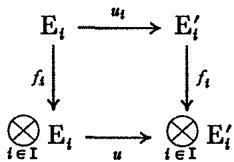
\includegraphics[keepaspectratio]{images/part003_14ac730d.jpg}}

is commutative, \(f_{i}\) and \(f_{i}^{\prime}\) denoting the canonical homomorphisms.

It suffices to apply Proposition 8 to the homomorphism \(f_{i}^{\prime} \circ u_{i}\) .

The homomorphism \(u\) defined in the Corollary to Proposition 8 is denoted by \(\bigotimes_{i \in I} u_i\) . If \(J\) is any subset of \(I\) , Proposition 8 can be applied to the family \((f_i)_{i \in J}\) of canonical homomorphisms \(f_i: E_i \to \bigotimes_{i \in I} E_i = E\) ; a canonical homomorphism \(E_J \to E\) is derived which is also denoted by \(f_J\) and which, when \(J\) is finite, coincides with the homomorphism denoted thus above.

Now let \((x_{i})_{i\in \mathbf{I}}\) be an element of \(\prod_{i\in \mathbf{I}}\mathrm{E}_i\) such that the family \((x_{i} - e_{i})_{i\in \mathbf{I}}\) has finite support H. It is immediate that, if J and \(J^{\prime}\) are two finite subsets of I containing H, then

\[
f _ {J} ((x _ {i}) _ {i \in J}) = f _ {J ^ {\prime}} ((x _ {i}) _ {i \in J ^ {\prime}}).
\]

The common value of the \(f_{\mathbf{J}}((x_i)_{i \in \mathbf{J}})\) for the finite subsets \(\mathbf{J} \supset \mathbf{H}\) of \(\mathbf{I}\) is denoted by \(\bigotimes_{i \in \mathbf{I}} x_i\) .

PROPOSITION 9. Let \((\mathbf{E}_i)_{i\in \mathbf{I}}\) be a family of A-algebras and for each \(i\in \mathbf{I}\) let \(B_{i}\) be a basis of \(\mathbf{E}_i\) such that the unit element \(e_i\) belongs to \(\overline{\mathbf{B}}_i\) . Let \(\mathbf{B}\) be the set of elements of the form \(\bigotimes_{i\in \mathbf{I}}x_i\) , where \((x_{i})\) runs through the set of elements of \(\prod_{i\in \mathbf{I}}\mathbf{B}_i\) such that the family \((x_{i} - e_{i})\) has finite support. Then \(\mathbf{B}\) is a basis of the algebra \(\bigotimes_{i\in \mathbf{I}}\mathbf{E}_i\) and this basis contains the unit element \(e\) .

For every finite subset J of I, let \(B_{J}\) be the basis of \(E_{J} = \bigotimes_{i \in J} E_{i}\) the tensor product of the bases \(B_{i}\) for \(i \in J\) (II, §3, no. 9). It follows immediately from the definitions that B is the union of the \(f_{J}(B_{J})\) when J runs through \(\mathfrak{F}(I)\) and that \(f_{J^{\prime}J}(B_{J}) \subset B_{J^{\prime}}\) when \(J \subset J^{\prime}\) ; hence \((B_{J})\) is a direct system of subsets of the \(E_{J}\) and \(B = \varinjlim B_{J}\) ; the conclusion then follows from II, §6, no. 2, Corollary to Proposition 5.

The basis B is also called the tensor product of the bases \(B_{i}\) for \(i \in I\) ; when the conditions of Proposition 9 are fulfilled, the canonical homomorphisms \(f_{J}: E_{J} \to E = \bigotimes_{i \in I} E_{i}\) are injective for every subset J of I, for if \(B_{J}\) is the basis of \(E_{J}\) the tensor product of the \(B_{i}\) for \(i \in J\) , it is immediately verified that the restriction of \(f_{J}\) to \(B_{J}\) is injective and maps \(B_{J}\) onto a subset of B.

\subsection{COMMUTATION LEMMAS}

Lemma 1. Let \(\mathbf{A}\) be a commutative ring, \(\mathbf{E}\) an \(\mathbf{A}\) -algebra, \((x_{i})_{1\leqslant i\leqslant n}\) a finite sequence of elements of \(\mathbf{E}\) , \((\lambda_i)_{1\leqslant i\leqslant n}\) a finite sequence of elements of \(\mathbf{A}\) and \(y\) an element of \(\mathbf{E}\) ; suppose that

\[
x _ {i} y = \lambda_ {i} y x _ {i} \quad \text { for } 1 \leqslant i \leqslant n.\tag{13}
\]

Then

\[
\left(x _ {1} x _ {2} \dots x _ {n}\right) y = \left(\lambda_ {1} \lambda_ {2} \dots \lambda_ {n}\right) y \left(x _ {1} x _ {2} \dots x _ {n}\right).\tag{14}
\]

The lemma being trivial for \(n = 1\) , we argue by induction on \(n \geqslant 2\) . Now

\[
\begin{array}{r l} (x _ {1} x _ {2} \dots x _ {n}) y & = (x _ {1} \dots x _ {n - 1}) (x _ {n} y) \\ & = (x _ {1} \dots x _ {n - 1}) (\lambda_ {n} y x _ {n}) = \lambda_ {n} ((x _ {1} \dots x _ {n - 1}) y) x _ {n}, \end{array}
\]

which, by the induction hypothesis, is equal to

\[
\lambda_ {n} \left(\lambda_ {1} \dots \lambda_ {n - 1}\right) y \left(x _ {1} \dots x _ {n - 1}\right) x _ {n} = \left(\lambda_ {1} \dots \lambda_ {n - 1} \lambda_ {n}\right) y \left(x _ {1} \dots x _ {n - 1} x _ {n}\right),
\]

whence the lemma.

Lemma 2. Let A be a commutative ring, E an A-algebra and \((x_{i})_{1\leqslant i\leqslant n}\) and \((y_{i})_{1\leqslant i\leqslant n}\) two finite sequences of \(n\) elements of E; suppose that for \(1\leqslant j\leqslant i\leqslant n\) ,

\[
x _ {i} y _ {j} = \lambda_ {i j} y _ {j} x _ {i} \quad \text { with } \lambda_ {i j} \in A.\tag{15}
\]

Then

\[
\left(x _ {1} x _ {2} \dots x _ {n}\right) \left(y _ {1} y _ {2} \dots y _ {n}\right) = \left(\prod_ {i > j} \lambda_ {i j}\right) \left(x _ {1} y _ {1}\right) \left(x _ {2} y _ {2}\right) \dots \left(x _ {n} y _ {n}\right).\tag{16}
\]

The lemma being trivial for \(n = 1\) , we again argue by induction on \(n\) for \(n \geqslant 2\) . By virtue of Lemma 1,

\[
\begin{array}{r l} (x _ {1} \dots x _ {n}) (y _ {1} \dots y _ {n}) & = x _ {1} (x _ {2} \dots x _ {n}) y _ {1} (y _ {2} \dots y _ {n}) \\ & = \left(\prod_ {i > 1} \lambda_ {i 1}\right) (x _ {1} y _ {1}) (x _ {2} \dots x _ {n}) (y _ {2} \dots y _ {n}) \end{array}
\]

and it then suffices to apply the induction hypothesis to obtain (16).

For every family \(\lambda = (\lambda_{ij})\) of elements of A, with \(1 \leqslant j < i \leqslant n\) , and for every permutation \(\sigma \in \mathfrak{S}_n\) , we write

\[
\varepsilon_ {\sigma} (\lambda) = \prod_ {i > j, \sigma^ {- 1} (i) < \sigma^ {- 1} (j)} \lambda_ {i j} = \prod_ {i <   j, \sigma (i) > \sigma (j)} \lambda_ {\sigma (i), \sigma (j)}.\tag{17}
\]

Observe that, when \(\mathbf{A} = \mathbf{Z}\) and \(\lambda_{ij} = -1\) for every ordered pair \((i,j)\) such that \(1 \leqslant j < i \leqslant n\) , \(\varepsilon_{\sigma}(\lambda)\) is just the signature \(\varepsilon_{\sigma}\) of the permutation \(\sigma\) (I, § 5, no. 7).

Lemma 3. Let A be a commutative ring, E an A-algebra, \((x_{i})_{1\leqslant i\leqslant n}\) a finite sequence of elements of E and suppose that, for every ordered pair \((i,j)\) of integers such that \(1\leqslant j < i\leqslant n\) ,

\[
x _ {i} x _ {j} = \lambda_ {i j} x _ {j} x _ {i} \quad \text { with } \lambda_ {i j} \in A.\tag{18}
\]

Then, for every permutation \(\sigma \in \mathfrak{S}_n\) ,

\[
x _ {\sigma (1)} x _ {\sigma (2)} \dots x _ {\sigma (n)} = \varepsilon_ {\sigma} (\lambda) x _ {1} x _ {2} \dots x _ {n}.\tag{19}
\]

The lemma is trivial for \(n = 1\) and \(n = 2\) ; we proceed by induction on \(n\) for \(n \geqslant 3\) . If \(\sigma(n) = n\) , relation (19) follows from the induction hypothesis. Suppose therefore that \(\sigma(n) = k, k \neq n\) , and let \(\tau\) be the permutation of \([1, n]\) defined by

\[
\left\{ \begin{array}{l l} \tau (i) = i & \text { for } i <   k \\ \tau (i) = i + 1 & \text { for } k \leqslant i <   n \\ \tau (n) = k. \end{array} \right.
\]

Let \(\pi = \tau^{-1} \circ \sigma\) ; the permutation \(\pi\) leaves \(n\) fixed; now \(\sigma = \tau \circ \pi\) and therefore, writing \(y_i = x_{\tau(i)}\) , \(y_{\pi(i)} = x_{\sigma(i)}\) . If \(i \neq n\) and \(j \neq n\) , the relations \(\pi(i) > \pi(j)\) and \(\sigma(i) > \sigma(j)\) are equivalent (since \(\tau\) is a strictly increasing mapping of \([1, n - 1]\) into \([1, n]\) . For \(i \neq n\) , \(j \neq n\) and \(\sigma(i) > \sigma(j)\) ,

\[
y _ {\pi (i)} y _ {\pi (j)} = x _ {\sigma (i)} x _ {\sigma (j)} = \lambda_ {\sigma (i), \sigma (j)} x _ {\sigma (j)} x _ {\sigma (i)} = \lambda_ {\sigma (i), \sigma (j)} y _ {\pi (j)} y _ {\pi (i)}
\]

whence, by the induction hypothesis (using the fact that \(\pi(n) = n\) ):

\[
y _ {\pi (1)} y _ {\pi (2)} \dots y _ {\pi (n)} = \left(\prod_ {i <   j <   n, \sigma (i) > \sigma (j)} \lambda_ {\sigma (i), \sigma (j)}\right) y _ {1} y _ {2} \dots y _ {n}
\]

that is

\[
x _ {\sigma (1)} x _ {\sigma (2)} \dots x _ {\sigma (n)} = \left(\prod_ {i <   j <   n, \sigma (i) > \sigma (j)} \lambda_ {\sigma (i), \sigma (j)}\right) x _ {\tau (1)} \dots x _ {\tau (n)}.\tag{20}
\]

Now

\[
x _ {\tau (1)} \dots x _ {\tau (n)} = x _ {1} \dots x _ {k - 1} x _ {k + 1} \dots x _ {n} x _ {k}
\]

and this, by Lemma 1, is equal to

\[
\left(\prod_ {j > k} \lambda_ {j k}\right) x _ {1} \dots x _ {n} = \left(\prod_ {\sigma (i) > \sigma (n)} \lambda_ {\sigma (i), \sigma (n)}\right) x _ {1} \dots x _ {n}.\tag{21}
\]

Finally, (20) and (21) give

\[
x _ {\sigma (1)} \dots x _ {\sigma (n)} = \alpha . x _ {1} \dots x _ {n}
\]

with

\[
\begin{array}{l} \alpha = \left(\prod_ {i <   j <   n, \sigma (i) > \sigma (j)} \lambda_ {\sigma (i), \sigma (j)}\right) \cdot \left(\prod_ {i <   n, \sigma (i) > \sigma (n)} \lambda_ {\sigma (i), \sigma (n)}\right) \\ = \prod_ {i <   j, \sigma (i) > \sigma (j)} \lambda_ {\sigma (i), \sigma (j)} = \varepsilon_ {\sigma} (\lambda) \end{array}
\]

which completes the proof of Lemma 3.

\subsection{TENSOR PRODUCT OF GRADED ALGEBRAS RELATIVE TO COMMUTATION FACTORS}

DEFINITION 6. Let \((\Delta_{i})_{i\in I}\) be a finite family of commutative monoids written additively. A system of commutation factors over the \(\Delta_{i}\) with values in a commutative ring A is a system of mappings \(\varepsilon_{ij}:\Delta_i\times \Delta_j\to \mathbf{A}\) , where \(i\in \mathbf{I}, j\in \mathbf{I}, i\neq j\) satisfying the following conditions:

\[
\varepsilon_ {i j} \left(\alpha_ {i} + \alpha_ {i} ^ {\prime}, \beta_ {j}\right) = \varepsilon_ {i j} \left(\alpha_ {i}, \beta_ {j}\right) \varepsilon_ {i j} \left(\alpha_ {i} ^ {\prime}, \beta_ {j}\right)\tag{22}
\]

\[
\varepsilon_ {i j} \left(\alpha_ {i}, \beta_ {j} + \beta_ {j} ^ {\prime}\right) = \varepsilon_ {i j} \left(\alpha_ {i}, \beta_ {j}\right) \varepsilon_ {i j} \left(\alpha_ {i}, \beta_ {j} ^ {\prime}\right)\tag{23}
\]

\[
\varepsilon_ {i j} (\alpha_ {i}, \beta_ {j}) \varepsilon_ {j i} (\beta_ {j}, \alpha_ {i}) = 1,\tag{24}
\]

for all \(\alpha_{i},\alpha_{i}^{\prime}\) in \(\Delta_{i},\beta_{j},\beta_{j}^{\prime}\) in \(\Delta_j\).

If I is given a total ordering and the \(\Delta_{i}\) are groups, a system of commutation factors is defined over the \(\Delta_{i}\) by taking for every ordered pair \((i,j)\) such that i\textless j an arbitrary Z-bilinear mapping of \(\Delta_{i}\times\Delta_{j}\) into the (multiplicative) Z-module A* of invertible elements of the ring A and then writing

\[
\varepsilon_ {j i} (\beta_ {j}, \alpha_ {i}) = (\varepsilon_ {i j} (\alpha_ {i}, \beta_ {j})) ^ {- 1}
\]

for \(i < j\) .

Note that, since the \(\varepsilon_{ij}(\alpha_{i},\beta_{j})\) are invertible,

\[
\varepsilon_ {i j} (0, \beta_ {j}) = \varepsilon_ {i j} (\alpha_ {i}, 0) = 1,
\]

by virtue of (22) and (23).

Examples. (1) The trivial system of commutation factors consists of the \(\varepsilon_{ij}\) such that \(\varepsilon_{ij}(\alpha_i, \beta_j) = 1\) for all \(i, j, \alpha_i \in \Delta_i, \beta_j \in \Delta_j\) .

\begin{enumerate}
\def\labelenumi{(\arabic{enumi})}
\setcounter{enumi}{1}
\tightlist
\item
  If we take \(\mathbf{A} = \mathbf{Z}\) and \(\Delta_{i} = \mathbf{Z}\) for all \(i \in \mathbf{I}\) , a system of commutation factors is obtained by taking \(\varepsilon_{ij}(\alpha_i, \beta_j) = (-1)^{\alpha_i\beta_j}\) . Note that this number depends only on the parities of \(\alpha_{i}\) and \(\beta_{j}\) and the \(\varepsilon_{ij}\) can therefore be considered as commutation factors when certain of the \(\Delta_{i}\) are equal to \(\mathbf{Z}/2\mathbf{Z}\) and the others to \(\mathbf{Z}\) .
\end{enumerate}

These two examples are the most frequent cases encountered in applications.

PROPOSITION 10. Let A be a commutative ring and \((\Delta_{i})_{i\in I}\) a finite family of commutative monoids written additively; for each \(i\in I\) let \(\mathbf{E}_i\) be a graded A-algebra of type \(\Delta_i\) . Finally, let \((\varepsilon_{ij})\) be a system of commutation factors over the \(\Delta_i\) with values in A. Then there exist a graded A-algebra E of type \(\Delta = \prod_{i\in I}\Delta_i\) and for each \(i\in I\) an algebra homomorphism \(h_i:\mathbf{E}_i\to \mathbf{E}\) , with the following properties:

\begin{enumerate}
\def\labelenumi{(\roman{enumi})}
\item
  If \(\phi_{i}:\Delta_{i}\to\Delta\) is the canonical homomorphism, then \(h_{i}\) is a graded homomorphism (II, § 11, no. 2), in other words, \(h_{i}(E_{i}^{\alpha_{i}})\subset E^{\phi_{i}(\alpha_{i})}\) , where \((E_{i}^{\alpha_{i}})\) and \((E^{\alpha})\) denote the respective graduations on \(E_{i}\) and \(E\) .
\item
  If \(i \neq j\) and \(x_{i}\) (resp. \(x_{j}\) ) is a homogeneous element of \(\mathbf{E}_i\) (resp. \(\mathbf{E}_j\) ) of degree \(\alpha_i \in \Delta_i\) (resp. \(\beta_j \in \Delta_j\) ), then
\end{enumerate}

\[
h _ {i} (x _ {i}) h _ {j} (x _ {j}) = \varepsilon_ {i j} (\alpha_ {i}, \beta_ {j}) h _ {j} (x _ {j}) h _ {i} (x _ {i}).\tag{25}
\]

\begin{enumerate}
\def\labelenumi{(\roman{enumi})}
\setcounter{enumi}{2}
\tightlist
\item
  For every A-algebra \(\mathbf{F}\) and every system of homomorphisms \(f_{i}:\mathbf{E}_{i}\to \mathbf{F}\) satisfying the conditions
\end{enumerate}

\[
f _ {i} (x _ {i}) f _ {j} (x _ {j}) = \varepsilon_ {i j} (\alpha_ {i}, \beta_ {j}) f _ {j} (x _ {j}) f _ {i} (x _ {i}),\tag{26}
\]

where \(i, j, x_i, x_j, \alpha_i, \beta_j\) are as in (ii), then there exists one and only one algebra homomorphism \(f: \mathbf{E} \to \mathbf{F}\) such that \(f_i = f \circ h_i\) for all \(i \in \mathbf{I}\) . Moreover the underlying A-module of \(\mathbf{E}\) is the tensor product \(\bigotimes_{i \in \mathbf{I}} \mathbf{E}_i\) .

Consider the A-module \(E = \bigotimes_{i \in I} E_i\) ; it is identified with the direct sum of the submodules \(E^\alpha\) , where, for each \(\alpha = (\alpha_i) \in \Delta\) , we write \(E^\alpha = \bigotimes_{i \in I} E_i^{\alpha_i}\) ; the \(E^\alpha\) therefore form a graduation of type \(\Delta\) on the A-module E. We shall define on E a graded A-algebra structure of type \(\Delta\) . For this let I be given a total ordering; for every ordered pair of elements \(\alpha = (\alpha_i)\) , \(\beta = (\beta_i)\) of \(\Delta\) , we must first define an A-bilinear mapping of \(E^\alpha \times E^\beta\) into \(E^\alpha + \beta\) , or alternatively an A-linear mapping \(m_{\alpha\beta}\) of \(E^\alpha \otimes_A E^\beta\) into \(E^\alpha + \beta\) . We shall define \(m_{\alpha\beta}\) by the condition

\[
m _ {\alpha \beta} \left(\left(\bigotimes_ {i \in I} x _ {i}\right) \otimes \left(\bigotimes_ {i \in I} y _ {i}\right)\right) = \varepsilon (\alpha , \beta) \bigotimes_ {i \in I} (x _ {i} y _ {i})\tag{27}
\]

for \(x_{i}\in \mathrm{E}_{i}^{\alpha_{i}},y_{i}\in \mathrm{E}_{i}^{\beta_{i}}\) , where

\[
\varepsilon (\alpha , \beta) = \prod_ {i > j} \varepsilon_ {i j} (\alpha_ {i}, \beta_ {j}).\tag{28}
\]

The right hand side of (27) obviously belongs to \(\mathbf{E}^{\alpha +\beta}\) and the mapping \((x_{1},\ldots ,x_{n},y_{1},\ldots ,y_{n})\mapsto \varepsilon (\alpha ,\beta)\bigotimes_{i\in I}(x_{i}y_{i})\) is A-multilinear in the product of the \(\mathrm{E}_i^{\alpha_i}\) and the \(\mathrm{E}_i^{\beta_i}(1\leqslant i\leqslant n)\) . Then it must be proved that the multiplication thus defined on E is associative; now, if \(\gamma = (\gamma_{i})\) is a third element of \(\Delta\) and \(z_{i} \in \mathrm{E}_{i}^{\gamma_{i}}\) for \(1 \leqslant i \leqslant n\) , then

\[
\left(\left(\bigotimes_ {i} x _ {i}\right) \left(\bigotimes_ {i} y _ {i}\right)\right) \left(\bigotimes_ {i} z _ {i}\right) = \varepsilon (\alpha + \beta , \gamma) \varepsilon (\alpha , \beta) \bigotimes_ {i} (x _ {i} y _ {i} z _ {i})
\]

\[
\left(\bigotimes_ {i} x _ {i}\right) \left(\left(\bigotimes_ {i} y _ {i}\right) \left(\bigotimes_ {i} z _ {i}\right)\right) = \varepsilon (\alpha , \beta + \gamma) \varepsilon (\beta , \gamma) \bigotimes_ {i} (x _ {i} y _ {i} z _ {i})
\]

and it reduces to verifying the identity

\[
\varepsilon (\alpha + \beta , \gamma) \varepsilon (\alpha , \beta) = \varepsilon (\alpha , \beta + \gamma) \varepsilon (\beta , \gamma).
\]

But the latter follows immediately from the relations

\[
\varepsilon (\alpha + \beta , \gamma) = \varepsilon (\alpha , \beta) \varepsilon (\beta , \gamma)
\]

\[
\varepsilon (\alpha , \beta + \gamma) = \varepsilon (\alpha , \beta) \varepsilon (\alpha , \gamma)
\]

themselves immediate consequences of the definition (28) and (22) and (23).

If, for all \(i \in \mathbf{I}\) , \(e_i\) denotes the unit element of \(\mathbf{E}_i\) , we know that \(e_i\) is homogeneous of degree 0 (§ 3, no. 1), hence \(e = \bigotimes_{i \in \mathbf{I}} e_i\) is homogeneous of degree 0 and it follows from (27), (28) and the relations

\[
\varepsilon_ {i j} (\alpha_ {i}, 0) = \varepsilon_ {i j} (0, \beta_ {j}) = 1
\]

that \(e\) is unit element of \(\mathbf{E}\) , which completes the definition on \(\mathbf{E}\) of the desired graded A-algebra structure. Then take \(h_i(x_i) = x_i \otimes \bigotimes_{j \neq i} e_j\) ; to verify that \(h_i(x_i x_i') = h_i(x_i) h_i(x_i')\) for \(x_i, x_i'\) in \(\mathbf{E}_i\) , attention may be confined to the case where \(x_i\) and \(x_i'\) are homogeneous and then this relation follows immediately from (27) and the relations \(\varepsilon_{ij}(\alpha_i, 0) = \varepsilon_{ij}(0, \beta_j) = 1\) ; the same relations and (24) prove also that the \(h_i\) satisfy conditions (i) and (ii) of the statement and that

\[
\bigotimes_ {i \in I} x _ {i} = \prod_ {i \in I} h _ {i} (x _ {i})\tag{29}
\]

where the right hand side is the product of the ordered sequence \((h_i(x_i))_{i\in I}\) in E with the given total ordering on I (I, § 1, no. 2) (it suffices to argue by induction on the number of \(x_{i}\) (assumed homogeneous) distinct from the \(e_i\) ).

It remains to prove condition (iii); note that the mapping

\[
(x _ {i}) _ {i \in I} \mapsto \prod_ {i \in I} f _ {i} (x _ {i}),
\]

where the right hand side is the product of the ordered sequence \((f_{i}(x_{i}))_{i\in\mathbf{I}}\) with the given total ordering on I, is A-multilinear. Then there exists one and only one A-linear mapping \(f: E \rightarrow F\) such that

\[
f \left(\bigotimes_ {i \in I} x _ {i}\right) = \prod_ {i \in I} f _ {i} (x _ {i}).\tag{30}
\]

Clearly \(f(e)\) is the unit element of \(\mathbf{F}\) and \(f \circ h_i = f_i\) ; to verify that \(f\) is an algebra homomorphism, in other words that \(f(x)f(y) = f(xy)\) for \(x, y\) in \(\mathbf{E}\) , attention may be confined, by linearity, to the case where \(x = \bigotimes_{i \in \mathbf{I}} x_i\) and \(y = \bigotimes_{i \in \mathbf{I}} y_i\) , \(x_i\) (resp. \(y_i\) ) being homogeneous of degree \(\alpha_i\) (resp. \(\beta_i\) ) for all \(i \in \mathbf{I}\) . The relation to be verified then reduces, by (27), to

\[
\left(\prod_ {i \in \mathrm{I}} f _ {i} (x _ {i})\right) \left(\prod_ {i \in \mathrm{I}} f _ {i} (y _ {i})\right) = \varepsilon (\alpha , \beta) \prod_ {i \in \mathrm{I}} \left(f _ {i} (x _ {i}) f _ {i} (y _ {i})\right).
\]

But, taking account of relations (26), this is a consequence of Lemma 2 of no. 6.

Clearly the algebra E and the canonical mapping \(\psi: \bigotimes_{i \in I} E_i \to E\) constitute a solution of the universal mapping problem (Set Theory, IV, § 3, no. 1), where \(\Sigma\) is the species of A-algebra structure and the \(\alpha\) -mappings \(\prod_{i} f_i\) from \(\prod_{i} E_i\) to an A-algebra, satisfying conditions (26).

For a fixed total ordering on I, the graded algebra E defined in the proof of Proposition 10 will be called a graded tensor \(\varepsilon\) -product of type \(\Delta\) of the family \((\mathrm{E}_i)_{i\in \mathbf{I}}\) of graded algebras of type \(\Delta_i\) and will be denoted by \({}^{\varepsilon}\bigotimes_{i\in \mathbf{I}}\mathrm{E}_i\) (if no confusion can arise over the ordering on I); similarly, the homomorphism \(f:\mathrm{E}\to \mathrm{F}\) defined in the proof of Proposition 10 will be denoted by \({}^{\varepsilon}\bigotimes_{i\in \mathbf{I}}f_i\) . The homomorphisms \(h_i\) are called canonical. We also write \({}^{\varepsilon}\mathrm{G}^{\otimes n}\) when \(\mathbf{I} = [1,n]\) and all the \(\mathrm{E}_i\) are equal to the same algebra G.

Remarks. (1) We recover the tensor product of algebras defined in no. 1 (with moreover the graduation the tensor product of those of its factors) taking \(\varepsilon_{ij}(\alpha_i, \beta_j) = 1\) for all \(i, j, \alpha_i\) and \(\beta_j\) .

\begin{enumerate}
\def\labelenumi{(\arabic{enumi})}
\setcounter{enumi}{1}
\tightlist
\item
  Suppose that all the \(\Delta_{i}\) are equal to \(\mathbf{Z}\) and write \(\varepsilon_{ij}(\alpha_i, \beta_j) = (-1)^{\alpha_i \beta_j}\) ; the tensor \(\varepsilon\) -product \({}^{\varepsilon}\bigotimes_{i \in I} E_i\) corresponding to this system of commutation factors is then called the skew tensor product of the graded algebras \(E_i\) of type \(\mathbf{Z}\) and denoted by \({}^{g}\bigotimes_{i \in I} E_i\) (or \(E{}^{g} \otimes_A F\) for two algebras, or \({}^{g} G^{\otimes n}\) instead of \({}^{\varepsilon} G^{\otimes n}\) ).
\end{enumerate}

COROLLARY 1. In the notation of Proposition 10, suppose further that F is a graded A-algebra of type \(\Delta\) and that each \(f_{i}\) is a graded algebra homomorphism relative to \(\phi_{i}:\Delta_{i}\to\Delta\) ; then \(f={}^{\varepsilon}\bigotimes_{i}f_{i}\) is a graded algebra homomorphism.

This follows immediately from the definition of \(f\) and the fact that

\[
\sum_ {i \in I} \phi_ {i} (\alpha_ {i}) = (\alpha_ {i})
\]

by definition of the \(\phi_{i}\) .

It is therefore seen that \((\mathrm{E},\psi)\) is also a solution of another universal mapping problem, where this time \(\Sigma\) is the species of graded A-algebra structure of type \(\Delta\) , the morphisms being graded algebra homomorphisms of type \(\Delta\) and the \(\alpha\) -mappings the mappings \(\prod_{i}f_{i}\) , where, in addition to conditions (26), it is assumed that \(f_{i}\) is a graded algebra homomorphism relative to \(\phi_{i}\) .

COROLLARY 2. Let \((\mathbf{E}_i)_{i\in \mathbf{I}}\) , \((\mathbf{F}_i)_{i\in \mathbf{I}}\) be two finite families of A-algebras, with \(\mathbf{E}_i\) and \(\mathbf{F}_i\) graded of type \(\Delta_i\) for all \(i\in \mathbf{I}\) . For each \(i\in \mathbf{I}\) , let \(g_i:\mathbf{E}_i\to \mathbf{F}_i\) be a graded algebra homomorphism of type \(\Delta_i\) . Then, if \(h_i:\mathbf{E}_i\to {}^{\varepsilon}\bigotimes_{i\in \mathbf{I}}\mathbf{E}_i\) and \(h_i':\mathbf{F}_i\to {}^{\varepsilon}\bigotimes_{i\in \mathbf{I}}\mathbf{F}_i\) are the canonical homomorphisms, there exists one and only one homomorphism of graded A-algebras of type \(\Delta\) , \(g: {}^{\varepsilon}\bigotimes_{i\in \mathbf{I}}\mathbf{E}_i\to {}^{\varepsilon}\bigotimes_{i\in \mathbf{I}}\mathbf{F}_i\) such that \(g\circ h_i = h_i'\circ g_i\) for all \(i\in \mathbf{I}\) . Also, if each \(g_i\) is bijective, so is \(g\) .

It suffices to apply Corollary 1 to \(f_{i} = h_{i}^{\prime} \circ g_{i}\) , noting that conditions (26) then follow from relations (25) applied to the \(h_{i}^{\prime}\) .

The homomorphism defined in Corollary 2 is also denoted by \({}^{\varepsilon}\bigotimes_{i} g_{i}\) (if no confusion can arise); if, for each \(i \in I\) , \(G_{i}\) is a third graded A-algebra of type \(\Delta_{i}\) and \(g_{i}^{\prime}: F_{i} \to G_{i}\) a graded algebra homomorphism, then

\[
\left(^ {\varepsilon} \bigotimes_ {i} g _ {i} ^ {\prime}\right) \circ \left(^ {\varepsilon} \bigotimes_ {i} g _ {i}\right) = ^ {\varepsilon} \bigotimes_ {i} \left(g _ {i} ^ {\prime} \circ g _ {i}\right),\tag{31}
\]

as follows immediately from (30).

In the case of a skew tensor product of graded algebras of type \(\mathbf{Z}\) , we write \({}^{g}\bigotimes_{i}f_{i}\) instead of \({}^{\varepsilon}\bigotimes_{i}f_{i}\) for homomorphisms \(f_{i}: \mathrm{E}_{i} \to \mathrm{F}_{i}\) of graded algebras of type \(\mathbf{Z}\) ; when \(\mathrm{I} = \{1, 2\}\) , this homomorphism is also denoted by \(f_{1}{}^{g}\otimes f_{2}\) ; when \(\mathrm{I} = [1, n]\) and all the \(\mathrm{E}_{i}\) (resp. \(\mathrm{F}_{i}\) ) are equal and all the \(f_{i}\) equal to the same homomorphism \(f\) , we write \({}^{g}f^{\otimes n}\) .

Remark. In the proof of Proposition 10, a total ordering on I was used to define an algebra structure on the tensor product \(\bigotimes_{i\in I}E_i\) of the A-modules

\(E_{i}\) . If the ordering on I is changed, another multiplicative structure arises on \(\bigotimes_{i\in I}E_{i}\) , but the new algebra thus obtained is canonically isomorphic to the above, since both are solutions of the same universal mapping problem. For example, when \(I=\{1,2\}\) , the canonical isomorphism of the algebra \(E_{1}{}^{\varepsilon}\otimes_{A}E_{2}\) onto the algebra \(E_{2}{}^{\varepsilon}\otimes_{A}E_{1}\) maps \(x_{1}\otimes x_{2}\) to \(\varepsilon_{2,1}(\alpha,\beta)x_{2}\otimes x_{1}\) , where \(x_{1}\) is homogeneous of degree \(\alpha\) and \(x_{2}\) homogeneous of degree \(\beta\) .

Let J be a subset of I and, for each \(i \in J\) , consider the canonical homomorphism \(h_{i}: E_{i} \to {}^{\varepsilon}\bigotimes_{i \in I} E_{i} = E\) . By virtue of relations (25) a canonical homomorphism \(h: E' = {}^{\varepsilon}\bigotimes_{i \in J} E_{i} \to E\) is derived canonically (by Proposition 10) from these homomorphisms, such that, for all \(i \in J\) , \(h_{i}' = h \circ h_{i}\) , \(h_{i}'\) being the canonical homomorphism \(E_{i} \to E'\) . Taking the total ordering on J induced by that chosen on I, we obtain

\[
h \left(\bigotimes_ {i \in J} x _ {i}\right) = \prod_ {i \in I} h _ {i} \left(x _ {i}\right) = \bigotimes_ {i \in I} x _ {i} ^ {\prime}
\]

where the middle term is the product of the ordered sequence \((h_i(x_i))_{i\in J}\) and where, in the right hand term, \(x_{i}^{\prime} = x_{i}\) for \(i\in J\) , \(x_{i}^{\prime} = e_{i}\) for \(i\notin J\) .

PROPOSITION 11. (``associativity'' of the tensor \(\varepsilon\) -product). In the notation of Proposition 10, let \((J_{\lambda})_{\lambda \in L}\) be a partition of I and write \(\Delta_{\lambda}' = \prod_{i \in J_{\lambda}} \Delta_i\) for all \(\lambda \in L\) . Let \(E_{\lambda}'\) be a graded tensor \(\varepsilon\) -product of type \(\Delta_{\lambda}'\) of the family \((E_i)_{i \in J_{\lambda}}\) (for some total ordering chosen on \(J_{\lambda}\) ). On the other hand, for \(\lambda, \mu\) in L and \(\lambda \neq \mu\) , we write, for \(\alpha_{\lambda}' = (\alpha_i)_{i \in J_{\lambda}}, \beta_{\mu}' = (\beta_j)_{j \in J_{\mu}}\) ,

\[
\varepsilon_ {\lambda \mu} ^ {\prime} (\alpha _ {\lambda} ^ {\prime}, \beta_ {\mu} ^ {\prime}) = \prod_ {i \in J _ {\lambda}, j \in J _ {\mu}} \varepsilon_ {i j} (\alpha_ {i}, \beta_ {j}).\tag{32}
\]

Then \((\varepsilon_{\lambda \mu}^{\prime})\) is a system of commutation factors over the \(\Delta_{\lambda}^{\prime}\) with values in A and there exists one and only one homomorphism of graded algebras of type \(\Delta, v: {}^{\varepsilon'}\bigotimes_{\lambda \in L} E_{\lambda}^{\prime} \to {}^{\varepsilon}\bigotimes_{i \in I} E_{i}\) , such that

\[
v \left(\bigotimes_ {\lambda \in L} \left(\bigotimes_ {i \in J _ {\lambda}} x _ {i}\right)\right) = \bigotimes_ {i \in I} x _ {i}\tag{33}
\]

for all \((x_{i})\in \prod_{i\in \mathbf{I}}\mathrm{E}_{i}\) , provided that the total ordering is taken on \(\mathbf{I}\) which induces on each \(\mathbf{J}_{\lambda}\) the chosen total ordering, and which is such that, for \(\lambda < \mu\) in \(\mathbf{L}\) , \(i\in \mathbf{J}_{\lambda}\) and \(j\in \mathbf{J}_{\mu}\) , \(i < j\) .

The fact that the \(\varepsilon_{\lambda \mu}'\) form a system of commutation factors is trivial. Let \(h_{i,\lambda}:\mathrm{E}_i\to \mathrm{E}_{\lambda}', h_{\lambda}':\mathrm{E}_{\lambda}'\to {}^{\varepsilon'}\bigotimes_{\lambda \in L}\mathrm{E}_{\lambda}'\) be the canonical homomorphisms (for \(\lambda \in L\) , \(i\in \mathbf{J}_{\lambda}\) ) and write \(h_i'' = h_\lambda' \circ h_{i,\lambda}\) ; it will suffice by virtue of the uniqueness of the solution of a universal mapping problem, to show that \({}^{\varepsilon'}\bigotimes_{\lambda \in L} E_{\lambda}'\) and the \(h_i''\) satisfy the conditions of Proposition 10. Now, for all \(\lambda \in L\) , let \(f_{\lambda}': E_{\lambda}' \to F\) be the unique algebra homomorphism such that \(f_{\lambda}' \circ h_{i,\lambda} = f_i\) for all \(i \in J_{\lambda}\) . We show that, for \(\lambda \neq \mu\) , \(\alpha_{\lambda}' = (\alpha_i)_{i \in J_{\lambda}}\) , \(\beta_{\mu}' = (\beta_j)_{j \in J_{\mu}}\) ,

\[
f _ {\lambda} ^ {\prime} (x _ {\lambda} ^ {\prime}) f _ {\mu} ^ {\prime} (x _ {\mu} ^ {\prime}) = \varepsilon_ {\lambda \mu} ^ {\prime} (\alpha_ {\lambda} ^ {\prime}, \beta_ {\mu} ^ {\prime}) f _ {\mu} ^ {\prime} (x _ {\mu} ^ {\prime}) f _ {\lambda} ^ {\prime} (x _ {\lambda} ^ {\prime})\tag{34}
\]

for \(x_{\lambda}^{\prime} \in \mathrm{E}_{\lambda}^{\prime}\) (resp. \(x_{\mu}^{\prime} \in \mathrm{E}_{\mu}^{\prime}\) ) homogeneous of degree \(\alpha_{\lambda}^{\prime}\) (resp. \(\beta_{\mu}^{\prime}\) ); it suffices, by linearity, to verify it when \(x_{\lambda}^{\prime} = \bigotimes_{i \in J_{\lambda}} x_{i}\) , \(x_{\mu}^{\prime} = \bigotimes_{j \in J_{\mu}} x_{j}\) , \(x_{i}\) (resp. \(x_{j}\) ) being homogeneous of degree \(\alpha_{i}\) (resp. \(\beta_{j}\) ) in \(E_{i}\) (resp. \(E_{j}\) ) for \(i \in J_{\lambda}, j \in J_{\mu}\) . But this follows from formula (30) which defines the \(f_{\lambda}^{\prime}\) and Lemma 3 of no. 6, taking account of hypothesis (26) and definition (32). There is therefore one and only one algebra homomorphism \(f: ^{\varepsilon'} \bigotimes_{\lambda \in L} E_{\lambda}' \to F\) such that \(f \circ h_{\lambda}' = f_{\lambda}'\) for all \(\lambda \in L\) ; whence \(f \circ h_{i}' = f_{i}\) for all \(i \in I\) and the uniqueness of \(f\) is trivial.

\subsection{TENSOR PRODUCT OF GRADED ALGEBRAS OF THE SAME TYPES}

Assuming the hypotheses of no. 7, Proposition 10 hold, suppose further that all the \(\Delta_{i}\) are equal to the same commutative monoid \(\Delta_{0}\) ; we can then consider on the tensor \(\varepsilon\) -product \({}^{\varepsilon}\bigotimes_{i\in I}E_{i}\) the total graduation of type \(\Delta_{0}\) , associated with the graduation of type \(\Delta = \Delta_{0}^{I}\) on this algebra (II, § 11, no. 1); we shall call \({}^{\varepsilon}\bigotimes_{i\in I}E_{i}\) , with this graduation, a graded tensor \(\varepsilon\) -product of type \(\Delta_{0}\) of the family \((E_{i})_{i\in I}\) of graded algebras of type \(\Delta_{0}\) .

Always preserving the notation of Proposition 10 of no. 7, suppose that F is also a graded A-algebra of type \(\Delta_0\) and that the \(f_i\) are homomorphisms of graded algebras of type \(\Delta_0\) . Then \(f: {}^{\varepsilon}\bigotimes_{i \in I} E_i \to F\) is also a homomorphism of graded algebras of type \(\Delta_0\) : for it follows from formula (30) (no. 7) that if \(x_i\) is homogeneous and of degree \(\alpha_i \in \Delta_0\) , \(\bigotimes_{i \in I} x_i\) and \(\prod_{i \in I} f_i(x_i)\) are both homogeneous of degree \(\sum_{i \in I} \alpha_i \in \Delta_0\) .

It can therefore be said that \(\bigotimes_{i\in I}E_i\) , with the total graduation of type \(\Delta_0\) , constitutes, together with the canonical mapping \(\psi\) , a solution of a third universal mapping problem, where \(\Sigma\) is the species of graded A-algebra of type \(\Delta_0\) , the morphisms are homomorphisms of graded algebras of type \(\Delta_0\) and the \(\alpha\) -mappings are the mappings \(\prod_{i}f_{i}\) , where, in addition to conditions (26) (of no. 7), it is assumed that each \(f_{i}\) is a homomorphism of graded algebras of type \(\Delta_0\) .

For every subset J of I, the canonical homomorphism \({}^{\varepsilon}\bigotimes_{i\in J}E_i\to {}^{\varepsilon}\bigotimes_{i\in I}E_i\) (no. 7) is, in fact, a homomorphism of graded algebras of type \(\Delta_0\) , as follows immediately from the above.

PROPOSITION 12. (``associativity'' of the tensor \(\varepsilon\) -product of graded algebras of the same types). With the notation of Proposition 10 of no. 7, suppose that all the \(\Delta_{i}\) are equal to the same monoid \(\Delta_{0}\) ; let \((J_{\lambda})_{\lambda \in L}\) be a partition of I. With the notation of Proposition 11 of no. 7, suppose that the right hand side of formula (32) (no. 7) depends only on the sums \(\alpha_{\lambda}^{\prime \prime} = \sum_{i \in J_{\lambda}} \alpha_{i}, \beta_{\mu}^{\prime \prime} = \sum_{j \in J_{\mu}} \beta_{j}\) , for every ordered pair \((\lambda, \mu)\) of distinct indices, all \(\alpha_{\lambda}^{\prime} \in \Delta_{\lambda}^{\prime}\) and all \(\beta_{\mu}^{\prime} \in \Delta_{\mu}^{\prime}\) ; let \(\varepsilon_{\lambda \mu}^{\prime \prime}(\alpha_{\lambda}^{\prime \prime}, \beta_{\mu}^{\prime \prime})\) denote the right hand side of (32). Then \((\varepsilon_{\lambda \mu}^{\prime \prime})\) is a system of commutation factors over the family \((\Delta_{\lambda}^{\prime \prime})_{\lambda \in L}\) , where \(\Delta_{\lambda}^{\prime \prime} = \Delta_{0}\) for all \(\lambda \in L\) . If \(E_{\lambda}^{\prime \prime}\) is the graded tensor \(\varepsilon\) -product of type \(\Delta_{0}\) of the family \((E_{i})_{i \in J_{\lambda}}\) , there exists one and only one isomorphism of graded algebras of type \(\Delta_{0}\) , \(w: {}^{\varepsilon}\bigotimes_{\lambda \in L} E_{\lambda}^{\prime \prime} \to {}^{\varepsilon}\bigotimes_{i \in I} E_{i}\) , such that

\[
w \left(\bigotimes_ {\lambda \in L} \left(\bigotimes_ {i \in J _ {\lambda}} x _ {i}\right)\right) = \bigotimes_ {i \in I} x _ {i}\tag{35}
\]

provided that total orderings are chosen on the \(\mathbf{J}_{\lambda}\) and on \(\mathbf{I}\) as described in no. 7, Proposition 11.

By the hypothesis, for \(\gamma\) , \(\delta\) in \(\Delta_0\) , \(\varepsilon_{\lambda \mu}''(\gamma, \delta) = \varepsilon_{i_0 j_0}(\gamma, \delta)\) for some \(i_0 \in J_\lambda\) and some \(j_0 \in J_\mu\) , as is seen by considering the elements \(\alpha_\lambda' = (\alpha_i)_{i \in J_\lambda}\) and \(\beta_\mu' = (\beta_j)_{j \in J_\mu}\) such that \(\alpha_{i_0} = \gamma\) , \(\alpha_i = 0\) for \(i \neq i_0\) , \(\beta_{j_0} = \delta\) , \(\beta_j = 0\) for \(j \neq j_0\) ; it follows immediately that the \(\varepsilon_{\lambda \mu}''\) form a system of commutation factors. The rest of the proof is then analogous to that of Proposition 11 (no. 7) and is left to the reader.

Note that the additional hypotheses of Proposition 12 are fulfilled when \(\Delta_0 = \mathbf{Z}\) and that \((\varepsilon_{ij})\) is, either the trivial system of factors \((\varepsilon_{ij}(\alpha_i,\beta_j) = 1\) for all \(i,j)\) , or the system of factors defined by \(\varepsilon_{ij}(\alpha_i,\beta_j) = (-1)^{\alpha_i\beta_j}\) ; in the latter case, the right hand side of formula (32) is equal to \((-1)^{\gamma}\) , where \(\gamma = \sum_{i\in J_{\lambda},j\in J_{\mu}}\alpha_{i}\beta_{j} = \left(\sum_{i\in J_{\lambda}}\alpha_{i}\right)\left(\sum_{j\in J_{\mu}}\beta_{j}\right)\) .

Remarks. (1) Let I be an infinite indexing set and \(\Delta_0\) a commutative monoid; let \((\Delta_i)_{i \in I}\) denote the family such that \(\Delta_i = \Delta_0\) for all \(i\) and suppose given for every ordered pair of distinct indices \((i,j)\) of I a mapping \(\varepsilon_{ij} : \Delta_i \times \Delta_j \to A\) satisfying conditions (22), (23) and (24) (no. 7); this will also be called a system of commutation factors over the family \((\Delta_i)\) . Consider a family \((E_i)_{i \in I}\) of graded A-algebras of type \(\Delta_0\) ; for each finite subset J of I, let \(E_J\) denote a graded tensor \(\varepsilon\) -product of type \(\Delta_0\) of the subfamily \((E_i)_{i \in J}\) (with an arbitrary choice of a total ordering on J). If J, \(J'\) are two finite subsets of I such that \(J \subset J'\) , a canonical homomorphism of graded algebras of type \(\Delta_0\) , \(h_{J^{\prime}J}:E_{J}\to E_{J^{\prime}}\) , has been defined above and the uniqueness properties of these homomorphisms show immediately that if \(J\subset J^{\prime}\subset J^{\prime\prime}\) are three finite subsets of I, then \(h_{J^{\prime\prime}J}=h_{J^{\prime\prime}J^{\prime}}\circ h_{J^{\prime}J}\) . Thus there is a direct system \((E_{J},h_{J^{\prime}J})\) of graded algebras of type \(\Delta_{0}\) (§3, no. 3), whose indexing set is the right directed set \(\mathfrak{F}(I)\) of finite subsets of I. The graded algebra of type \(\Delta_{0}\) , the direct limit of this direct system (§3, no. 3), is called a graded tensor \(\varepsilon\) -product of type \(\Delta_{0}\) of the family \((E_{i})_{i\in I}\) ; it is also denoted by \({}^{\varepsilon}\bigotimes_{i\in I}E_{i}\) . When all the \(\Delta_{i}\) are equal to \(\mathbf{Z}\) and \(\varepsilon_{ij}(\alpha_{i},\beta_{j})=(-1)^{\alpha_{i}\beta_{j}}\) , the tensor product \({}^{\varepsilon}\bigotimes_{i\in I}E_{i}\) is also called the skew

tensor product of the family \((\mathbf{E}_{i})_{i\in\mathbb{I}}\) and is denoted by \({}^{g}\bigotimes_{i\in I}E_{i}\) . We leave to the reader the task of formulating and proving the proposition which generalizes Proposition 10 of no. 7 to the case where I is infinite, as Proposition 8 of no. 5 generalizes Proposition 5 of no. 2 to the case where I is infinite. Note that the underlying A-module of \({}^{\varepsilon}\bigotimes_{i\in I}E_{i}\) is the same as that underlying the (non-graded) tensor product of the family \((\mathbf{E}_{i})_{i\in\mathbb{I}}\) of non-graded algebras defined in no. 5.

\begin{enumerate}
\def\labelenumi{(\arabic{enumi})}
\setcounter{enumi}{1}
\tightlist
\item
  Let E be a graded A-algebra of type \(\Delta_0\) (where \(\Delta_0\) is a commutative monoid) and \(\rho: \mathbf{A} \to \mathbf{B}\) a ring homomorphism; the graduation on \(\rho^*(\mathbf{E})\) (II, §11, no. 5) is identical with the graduation on the graded tensor product \(\mathbf{B} \otimes_{\mathbf{A}} \mathbf{E}\) , where B has the trivial graduation.
\end{enumerate}

\subsection{ANTICOMMUTATIVE ALGEBRAS AND ALTERNATING ALGEBRAS}

DEFINITION 7. A graded A-algebra E of type Z is called anticommutative if for all non-zero homogeneous elements x, y of E

\[
x y = (- 1) ^ {\deg (x) \deg (y)} y x.\tag{36}
\]

The algebra \(\mathbf{E}\) is called alternating if it is anticommutative and also \(x^{2} = 0\) for every homogeneous element \(x\in \mathbf{E}\) of odd degree.

Remarks. (1) Let \(\mathbf{E}^{+}\) be the graded subalgebra of \(\mathbf{E}\) the direct sum of the \(\mathrm{E}_{2n}\) ( \(n \in \mathbf{Z}\) ); it follows from Definition 7 that if \(\mathbf{E}\) is anticommutative, \(\mathbf{E}^{+}\) is a subalgebra contained in the centre of \(\mathbf{E}\) (and hence commutative).

\begin{enumerate}
\def\labelenumi{(\arabic{enumi})}
\setcounter{enumi}{1}
\item
  Suppose that 2 is not a divisor of 0 in E; then if E is anticommutative E is alternating, since for \(x \in E\) homogeneous and of odd degree, \(x^{2} = -x^{2}\) by (36), whence \(2x^{2} = 0\) and \(x^{2} = 0\) by virtue of the hypothesis.
\item
  We shall study in detail in § 7 important examples of alternating algebras.
\end{enumerate}

Lemma 4. Let E be a graded algebra of type Z and S a set of homogeneous elements \(\neq0\) ; the set F of elements of E all of whose homogeneous components \(x\neq0\) satisfy relation (36) for all \(y\in S\) is a graded subalgebra of E.

It suffices to note that: (1) if \(x'\) , \(x''\) are two homogeneous elements of the same degree \(p\) , \(y\) a homogeneous element of degree \(q\) and \(x'y = (-1)^{pq}yx'\) , \(x''y = (-1)^{pq}yx''\) , then also \((x' + x'')y = (-1)^{pq}y(x' + x'')\) ; (2) if \(x'\) , \(x''\) are two homogeneous elements of respective degrees \(p'\) , \(p'', y\) a homogeneous element of degree \(q\) and \(x'y = (-1)^{p'q}yx'\) , \(x''y = (-1)^{p''q}yx''\) , then

\[
(x ^ {\prime} x ^ {\prime \prime}) y = (- 1) ^ {(p ^ {\prime} + p ^ {\prime \prime}) q} y (x ^ {\prime} x ^ {\prime \prime}).
\]

PROPOSITION 13. Let E be a graded A-algebra of type Z and S a generating system of the algebra E consisting of homogeneous elements \(\neq0\) ; for E to be anticommutative (resp. alternating), it is necessary and sufficient that (36) hold for all \(x\in S\) and \(y\in S\) (resp. that this condition holds and further that \(x^{2}=0\) for all x homogeneous of odd degree belonging to S).

We consider first the case of anticommutative algebras. By Lemma 4, the subalgebra F consisting of the elements all of whose homogeneous components \(x \neq 0\) satisfy (36) for all \(y \in S\) , contains all the elements of S and hence F = E. If now \(F'\) is similarly the subalgebra of E consisting of the elements all of whose homogeneous components \(x \neq 0\) satisfy (36) for every homogeneous element \(y \neq 0\) , it follows from the above that \(F'\) contains all the elements of S and hence \(F' = E\) , which completes the proof of the proposition in this case.

To prove the proposition in the case of alternating algebras, it can be assumed that E is already anticommutative; it is then immediate that every homogeneous element of odd degree in E is of the form \(\sum_{i} z_{i} x_{i}\) , where \(z_{i} \in E^{+}\) and \(x_{i} \in S\) is of odd degree (using the fact that \(E^{+}\) is contained in the centre of E); it follows that \(\left(\sum_{i} z_{i} x_{i}\right)^{2} = \sum_{i} z_{i}^{2} x_{i}^{2} + \sum_{i < j} z_{i} z_{j} (x_{i} x_{j} + x_{j} x_{i}) = 0\) since \(x_{i}^{2} = 0\) by hypothesis and \(x_{i} x_{j} + x_{j} x_{i} = 0\) by (36).

PROPOSITION 14. Let E and F be two graded A-algebras of type Z, both anticommutative (resp. alternating). Then the skew tensor product \(\mathbf{E}^{\mathbf{g}}\otimes_{\mathbf{A}}\mathbf{F}\) (no. 7) is an anticommutative (resp. alternating) algebra.

A generating system of \(E^{g} \otimes_{A} F\) consists of the \(x \otimes y\) , where x (resp. y) is a homogeneous element \(\neq 0\) of E (resp. F). Consider two such elements \(x \otimes y\) , \(x' \otimes y'\) , with \(\deg(x) = p\) , \(\deg(y) = q\) , \(\deg(x') = p'\) , \(\deg(y') = q'\) , so that \(x \otimes y\) is of degree \(p + q\) and \(x' \otimes y'\) of degree \(p' + q'\) . Then by definition (no. 7, formula (27)) and by virtue of (36),

\[
(x \otimes y) (x ^ {\prime} \otimes y ^ {\prime}) = (- 1) ^ {q p ^ {\prime}} (x x ^ {\prime}) \otimes (y y ^ {\prime})
\]

\[
\begin{array}{r l} (x ^ {\prime} \otimes y ^ {\prime}) (x \otimes y) & = (- 1) ^ {p q ^ {\prime}} (x ^ {\prime} x) \otimes (y ^ {\prime} y) \\ & = (- 1) ^ {p q ^ {\prime} + p p ^ {\prime} + q q ^ {\prime}} (x x ^ {\prime}) \otimes (y y ^ {\prime}) \end{array}
\]

and the criterion of Proposition 13 shows that \(\mathbf{E}^{\mathbf{g}}\otimes_{\mathbf{A}}\mathbf{F}\) is anticommutative since \(pq' + p p' + qq' - q p' \equiv (p + q)(p' + q')\) (mod. 2). If further E and F are alternating and \(p + q\) is odd, one of the numbers \(p, q\) is necessarily odd, hence \((x \otimes y)^2 = \pm (x^2) \otimes (y^2) = 0\) and Proposition 13 shows that \(E^g \otimes_A F\) is alternating.

COROLLARY. Let E be an anticommutative (resp. alternating) graded A-algebra of type Z. Then for every ring homomorphism \(\rho: \mathrm{A} \to \mathrm{B}\) , the graded B-algebra \(\rho^{*}(\mathrm{E})\) (no. 8, Remark 2) is anticommutative (resp. alternating).

The ring B with the trivial graduation can be considered as an alternating A-algebra and \(\rho^{*}(\mathbf{E}) = \mathbf{E}^{\mathfrak{g}}\otimes_{\mathbf{A}}\mathbf{B}\) , hence Proposition 14 can be applied.

Remark. Let E be an anticommutative graded A-algebra of type Z. Then the A-linear mapping of \(E \otimes_{A} E\) into E defined by multiplication of E (§1, no. 3) is a homomorphism of the graded A-algebra \(E^{g} \otimes_{A} E\) into E, for in the notation of Proposition 14, in the algebra E,

\[
(x y) (x ^ {\prime} y ^ {\prime}) = (- 1) ^ {q p ^ {\prime}} (x x ^ {\prime}) (y y ^ {\prime}).
\]

\section{TENSOR ALGEBRA, TENSORS}

\subsection{DEFINITION OF THE TENSOR ALGEBRA OF A MODULE}

Let A be a commutative ring and M an A-module. For every integer \(n \geqslant 0\) , the A-module the tensor product of n modules equal to M (also called the n-th tensor power of M) is denoted by \(\bigotimes^{n} M\) , or \(M^{\otimes n}\) , or \(T^{n}(M)\) , or \(T_{A}^{n}(M)\) , or \(\operatorname{Tens}^{n}(M)\) ; then \(T^{1}(M) = M\) ; also we write \(T^{0}(M) = A\) . The A-module the direct sum \(\bigoplus_{n \geqslant 0} T^{n}(M)\) is denoted by \(T(M)\) or \(\operatorname{Tens}(M)\) . We shall define a graded A-algebra structure of type N on \(T(M)\) , by defining for every ordered pair of integers \(p \geqslant 0\) , \(q \geqslant 0\) , an A-linear mapping

\[
m _ {p q} \colon \mathsf {T} ^ {p} (\mathbf {M}) \otimes_ {\mathbf {A}} \mathsf {T} ^ {q} (\mathbf {M}) \rightarrow \mathsf {T} ^ {p + q} (\mathbf {M})
\]

(§ 3, no. 1, Remark). For \(p > 0\) and \(q > 0\) , \(m_{pq}\) is the associativity isomorphism (II, § 3, no. 9) and, when \(p = 0\) (resp. \(q = 0\) ), \(m_{0,q}\) is the canonical isomorphism of \(A \otimes_A T^q(M)\) onto \(T^q(M)\) (resp. \(m_{p,0}\) is the canonical isomorphism of \(T^p(M) \otimes_A A\) onto \(T^p(M)\)) (II, § 3, no. 4, Proposition 4). Then, for \(x_t \in M\) , \(\alpha \in A\) ,

\[
\left\{ \begin{array}{r l} (x _ {1} \otimes \dots \otimes x _ {p}) \cdot (x _ {p + 1} \otimes \dots \otimes x _ {p + q}) & \\ = x _ {1} \otimes \dots \otimes x _ {p} \otimes x _ {p + 1} \otimes \dots \otimes x _ {p + q} \\ \alpha \cdot (x _ {1} \otimes \dots \otimes x _ {p}) = \alpha (x _ {1} \otimes \dots \otimes x _ {p}). \end{array} \right.\tag{1}
\]

It is immediate that the multiplication thus defined on \(\mathsf{T}(\mathbf{M})\) is associative and admits as unit element the unit element \(1\) of \(\mathbf{A} = \mathsf{T}^0 (\mathbf{M})\) .

DEFINITION 1. For every module M over a commutative ring A, the tensor algebra of M, denoted by T(M), or Tens(M), or \(\mathsf{T}_{\mathbf{A}}(\mathbf{M})\) , is the algebra \(\bigoplus_{n\geqslant 0}\mathsf{T}^n (\mathbf{M})\) with the multiplication defined in (1). The canonical injection \(\phi :\mathsf{T}^{1}(\mathbf{M})\to \mathsf{T}(\mathbf{M})\) (II, § 1, no. 12) (also denoted by \(\phi_{\mathbf{M}}\) ) is called the canonical injection of M into T(M).

PROPOSITION 1. Let E be a (unital) A-algebra and \(f:M\to E\) an A-linear mapping. There exists one and only one A-algebra homomorphism \(g:T(M)\to E\) such that \(f=g\circ\phi\) .

In other words, \((\mathsf{T}(\mathbf{M}), \phi)\) is a solution of the universal mapping problem (Set Theory, IV, §3, no. 1), where \(\Sigma\) is the species of A-algebra structure, the \(\alpha\) -mappings being the A-linear mappings from the module M to an A-algebra. Observe that here there is no question of a graduation on \(\mathsf{T}(\mathbf{M})\) .

For every finite family \((x_{i})_{1\leqslant i\leqslant n}\) of n elements of M, by definition of the product in T(M), \(x_{1}\otimes x_{2}\otimes\cdots\otimes x_{n}=\phi(x_{1})\phi(x_{2})\ldots\phi(x_{n})\) ; then necessarily \(g(x_{1}\otimes x_{2}\otimes\cdots\otimes x_{n})=f(x_{1})f(x_{2})\ldots f(x_{n})\) for \(n\geqslant1\) and \(g(\alpha)=\alpha e\) (if e is the unit element of E) for \(\alpha\in A\) , which proves the uniqueness of g. Conversely, note that, for all n\textgreater0, the mapping

\[
(x _ {1}, \dots , x _ {n}) \mapsto f (x _ {1}) f (x _ {2}) \dots f (x _ {n})
\]

of \(\mathbf{M}^n\) into \(\mathbf{E}\) is A-multilinear; hence there corresponds to it an A-linear mapping \(g_n: \mathsf{T}^n(\mathbf{M}) \to \mathbf{E}\) such that

\[
g \left(x _ {1} \otimes x _ {2} \otimes \dots \otimes x _ {n}\right) = f \left(x _ {1}\right) f \left(x _ {2}\right) \dots f \left(x _ {n}\right).\tag{2}
\]

Also we define the mapping \(g_0 \colon \mathsf{T}^0(\mathbf{M}) \to \mathbf{E}\) as equal to \(\eta_{\mathbf{E}}\) (§ 1, no. 3), in other words \(g_0(\alpha) = \alpha e\) for \(\alpha \in \mathbf{A}\) . Let \(g\) be the unique A-linear mapping of \(\mathsf{T}(\mathbf{M})\) into \(\mathbf{E}\) whose restriction to \(\mathsf{T}^n(\mathbf{M})\) is \(g_n\) ( \(n \geqslant 0\) ); it is immediate that \(g \circ \phi = g_1 = f\) and it remains to verify that \(g\) is an A-algebra homomorphism. By construction \(g(1) = e\) and it suffices by linearity to show that \(g(uv) = g(u)g(v)\) for \(u \in \mathsf{T}^p(\mathbf{M})\) and \(v \in \mathsf{T}^q(\mathbf{M})\) ( \(p > 0, q > 0\) ); now it follows from formulae (1) and (2) that this relation is true when \(u = x_1 \otimes x_2 \otimes \cdots \otimes x_p\) and \(v = x_{p+1} \otimes \cdots \otimes x_{p+q}\) (where the \(x_i\) belong to \(\mathbf{M}\) ). It is therefore true for \(u \in \mathsf{T}^p(\mathbf{M})\) and \(v \in \mathsf{T}^q(\mathbf{M})\) by linearity.

Remark. Suppose that \(\mathbf{E}\) is a graded A-algebra of type \(\mathbf{Z}\) , with graduation \((\mathbf{E}_n)\) , and suppose also that

\[
f (\mathbf {M}) \subset \mathrm{E} _ {1}.\tag{3}
\]

Then it follows from (2) that \(g(\mathsf{T}^p (\mathbf{M})) \subset \mathrm{E}_p\) for all \(p \geqslant 0\) and hence \(g\) is a graded algebra homomorphism.

\subsection{FUNCTORIAL PROPERTIES OF THE TENSOR ALGEBRA}

PROPOSITION 2. Let A be a commutative ring, M and N two A-modules and

\[
u: \mathbf {M} \rightarrow \mathbf {N}
\]

an A-linear mapping. There exists one and only one A-algebra homomorphism

\[
u ^ {\prime}: \mathsf {T} (\mathbf {M}) \rightarrow \mathsf {T} (\mathbf {N})
\]

such that the diagram

\pandocbounded{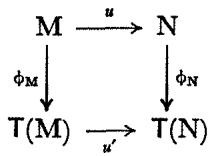
\includegraphics[keepaspectratio]{images/part003_fafbfb88.jpg}}

is commutative. Further, \(u'\) is a graded algebra homomorphism.

The existence and uniqueness of \(u'\) follow from no. 1, Proposition 1, applied to the algebra \(T(N)\) and the linear mapping \(\phi_N \circ u: M \to T(N)\) ; as

\[
u (\mathbf {M}) \subset \mathsf {T} ^ {1} (\mathbf {N}) = \mathbf {N},
\]

the fact that \(u'\) is a graded algebra homomorphism follows from the Remark of no. 1.

The homomorphism \(u'\) of Proposition 2 will henceforth be denoted by \(T(u)\) . If \(P\) is an A-module and \(v: N \to P\) an A-linear mapping, then

\[
\mathsf {T} (v \circ u) = \mathsf {T} (v) \circ \mathsf {T} (u)\tag{4}
\]

for \(\mathsf{T}(v)\circ \mathsf{T}(u)\) is an algebra homomorphism rendering commutative the diagram

\pandocbounded{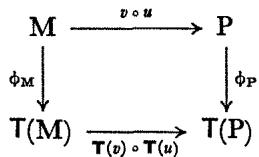
\includegraphics[keepaspectratio]{images/part003_f792dba1.jpg}}

\(\mathsf{T}(u)\) is sometimes called the canonical extension of u to \(\mathsf{T}(\mathbf{M})\) (which contains \(\mathbf{M} = \mathsf{T}^1(\mathbf{M})\) ). Note that the restriction \(\mathsf{T}^n(u): \mathsf{T}^n(\mathbf{M}) \to \mathsf{T}^n(\mathbf{N})\) is just the linear mapping \(u^{\otimes n} = u \otimes u \otimes \cdots \otimes u\) (n times), for

\[
\mathsf {T} ^ {n} (u) \left(x _ {1} \otimes \dots \otimes x _ {n}\right) = u \left(x _ {1}\right) \otimes \dots \otimes u \left(x _ {n}\right)
\]

since \(\mathsf{T}(u)\) is an algebra homomorphism and \(\mathsf{T}^{1}(u)=u\) ; the restriction \(\mathsf{T}^{0}(u)\) to A is the identity mapping. \(\mathsf{T}^{n}(u)\) is called the n-th tensor power of u.

PROPOSITION 3. If \(u: \mathbf{M} \to \mathbf{N}\) is a surjective A-linear mapping, the homomorphism \(\mathsf{T}(u): \mathsf{T}(\mathbf{M}) \to \mathsf{T}(\mathbf{N})\) is surjective and its kernel is the two-sided ideal of \(\mathsf{T}(\mathbf{M})\) generated by the kernel \(\mathbf{P} \subset \mathbf{M} \subset \mathsf{T}(\mathbf{M})\) of \(u\) .

\(T^{0}(u):T^{0}(M)\rightarrow T^{0}(N)\) is bijective and for every integer n\textgreater0,

\[
\mathbf {T} ^ {n} (u): \mathbf {T} ^ {n} (\mathbf {M}) \rightarrow \mathbf {T} ^ {n} (\mathbf {N})
\]

is surjective, as is seen by induction on \(n\) using II, § 3, no. 6, Proposition 6; the latter proposition also shows, by induction on \(n\) , that the kernel \(\mathfrak{S}_n\) of \(\mathsf{T}^n(u)\) is the submodule of \(\mathsf{T}^n(\mathbf{M})\) generated by the products

\[
x _ {1} \otimes x _ {2} \otimes \dots \otimes x _ {n}
\]

where at least one of the \(x_{i}\) belongs to \(\mathbf{P}\) . This shows that the kernel \(\mathfrak{S} = \bigoplus_{n\geqslant 1}\mathfrak{S}_n\) of \(\mathsf{T}(u)\) is the two-sided ideal generated by \(\mathbf{P}\) in \(\mathsf{T}(\mathbf{M})\) .

If \(u: \mathbf{M} \to \mathbf{N}\) is an injective linear mapping, it is not always true that \(\mathbf{T}(u)\) is an injective mapping (Exercise 1). However, this is true when \(u\) is an injection such that \(u(\mathbf{M})\) is a direct factor of \(\mathbf{N}\) , for then there exists a linear mapping \(v: \mathbf{N} \to \mathbf{M}\) such that \(v \circ u\) is the identity mapping on \(\mathbf{M}\) and therefore

\[
\mathsf {T} (v \circ u) = \mathsf {T} (v) \circ \mathsf {T} (u)
\]

is the identity mapping on \(\mathsf{T}(\mathbf{M})\) , hence \(\mathsf{T}(u)\) is injective and its image (isomorphic to \(\mathsf{T}(\mathbf{M})\) ) is a direct factor of \(\mathsf{T}(\mathbf{N})\) (II, §1, no. 9, Proposition 15). More precisely:

PROPOSITION 4. Let N and P be two submodules of an A-module M such that their sum \(N + P\) is a direct factor in M and their intersection \(N \cap P\) is a direct factor in N and in P. Then the homomorphisms \(\mathsf{T}(\mathbf{N}) \to \mathsf{T}(\mathbf{M})\) , \(\mathsf{T}(\mathbf{P}) \to \mathsf{T}(\mathbf{M})\) and

\[
\mathsf {T} (\mathbf {N} \cap \mathbf {P}) \rightarrow \mathsf {T} (\mathbf {M}),
\]

canonical extensions of the canonical injections, are injective; if \(\mathsf{T}(\mathbf{N})\) , \(\mathsf{T}(\mathbf{P})\) and \(\mathsf{T}(\mathbf{N} \cap \mathbf{P})\) are identified with subalgebras of \(\mathsf{T}(\mathbf{M})\) by means of these homomorphisms, then

\[
\mathsf {T} (\mathbf {N} \cap \mathbf {P}) = \mathsf {T} (\mathbf {N}) \cap \mathsf {T} (\mathbf {P}).\tag{5}
\]

By hypothesis, there exist submodules \(N' \subset N\) and \(P' \subset P\) such that \(N = N' \oplus (N \cap P)\) , \(P = P' \oplus (N \cap P)\) ; then

\[
\mathbf {N} + \mathbf {P} = \mathbf {N} ^ {\prime} \oplus \mathbf {P} ^ {\prime} \oplus (\mathbf {N} \cap \mathbf {P})
\]

and there exists by hypothesis a submodule \(M'\) of M such that

\[
\begin{array}{c} \mathbf {M} = \mathbf {M} ^ {\prime} \oplus (\mathbf {N} + \mathbf {P}) = \mathbf {M} ^ {\prime} \oplus \mathbf {N} ^ {\prime} \oplus \mathbf {P} ^ {\prime} \oplus (\mathbf {N} \cap \mathbf {P}) \\ = \mathbf {M} ^ {\prime} \oplus \mathbf {P} ^ {\prime} \oplus \mathbf {N} = \mathbf {M} ^ {\prime} \oplus \mathbf {N} ^ {\prime} \oplus \mathbf {P}. \end{array}
\]

In particular, \(N + P\) , N, P and \(N \cap P\) are direct factors in M, which implies, as has been seen above, that the canonical homomorphisms

\[
\begin{array}{l} \mathsf {T} (\mathbf {N} + \mathbf {P}) \to \mathsf {T} (\mathbf {M}), \qquad \mathsf {T} (\mathbf {N}) \to \mathsf {T} (\mathbf {M}), \\ \mathsf {T} (\mathbf {P}) \to \mathsf {T} (\mathbf {M}), \qquad \mathsf {T} (\mathbf {N} \cap \mathbf {P}) \to \mathsf {T} (\mathbf {M}) \end{array}
\]

are injective. The three algebras \(\mathsf{T}(\mathbf{N})\) , \(\mathsf{T}(\mathbf{P})\) and \(\mathsf{T}(\mathbf{N} \cap \mathbf{P})\) are thus identified with subalgebras of \(\mathsf{T}(\mathbf{N} + \mathbf{P})\) and the latter with a subalgebra of \(\mathsf{T}(\mathbf{M})\) ;

writing \(\mathbf{Q} = \mathbf{N} \cap \mathbf{P}\) , it remains to show that, if \(\mathsf{T}(\mathbf{Q})\) , \(\mathsf{T}(\mathbf{N}' \oplus \mathbf{Q})\) and \(\mathsf{T}(\mathbf{P}' \oplus \mathbf{Q})\) are identified with subalgebras of \(\mathsf{T}(\mathbf{N}' \oplus \mathbf{P}' \oplus \mathbf{Q})\) , then

\[
\mathsf {T} (\mathbf {N} ^ {\prime} \oplus \mathbf {Q}) \cap \mathsf {T} (\mathbf {P} ^ {\prime} \oplus \mathbf {Q}) = \mathsf {T} (\mathbf {Q}).\tag{6}
\]

Now, consider the commutative diagram

\pandocbounded{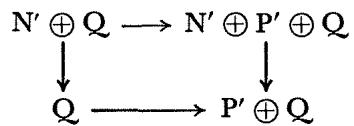
\includegraphics[keepaspectratio]{images/part003_8d12e188.jpg}}

where the horizontal arrows are the canonical injections and the vertical arrows the canonical projections. We derive a commutative diagram

\begin{enumerate}
\def\labelenumi{(\arabic{enumi})}
\setcounter{enumi}{6}
\tightlist
\item
\end{enumerate}

\pandocbounded{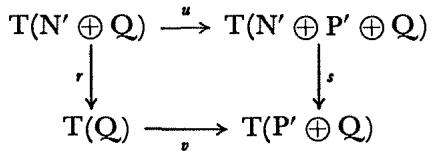
\includegraphics[keepaspectratio]{images/part003_389443db.jpg}}

where r and s are surjective homomorphisms (Proposition 3) and u and v injective homomorphisms. Hence, to prove (6), note that the right hand side is obviously contained in the left; it therefore suffices to verify that if

\[
x \in \mathsf {T} (\mathbf {N} ^ {\prime} \oplus \mathbf {Q}) \cap \mathsf {T} (\mathbf {P} ^ {\prime} \oplus \mathbf {Q}),
\]

then \(x \in \mathsf{T}(\mathsf{Q})\) . Now the definition of the homomorphism s shows that its restriction to \(\mathsf{T}(\mathsf{P}' \oplus \mathsf{Q})\) (identified with a subalgebra of \(\mathsf{T}(\mathsf{N}' \oplus \mathsf{P}' \oplus \mathsf{Q})\)) is the identity mapping; the hypothesis on x therefore implies that \(s(u(x)) = x\) . But then also \(v(r(x)) = x\) , in other words x belongs to the image of \(\mathsf{T}(\mathsf{Q})\) in \(\mathsf{T}(\mathsf{P}' \oplus \mathsf{Q})\) , which was to be proved.

Remark. Note in particular that the hypotheses of Proposition 4 always hold for arbitrary submodules N, P of M when A is a field (II, § 7, no. 3, Proposition 4). Moreover, if N ⊂ P and N ≠ P, then T \(^{n}\) (N) ≠ T \(^{n}\) (P) for all n ≥ 1, since if R is a complement of P in N, then T \(^{n}\) (P) ∩ T \(^{n}\) (R) = \{0\} by (4) and T \(^{n}\) (R) ≠ \{0\}.

COROLLARY. Let K be a commutative field and M a vector space over K. For every element \(z \in \mathsf{T}(\mathbf{M})\) , there exists a smallest vector space N of M such that \(z \in \mathsf{T}(\mathbf{N})\) and N is of finite rank over K.

It is understood in this statement that for every vector subspace P of M, \(T(P)\) is canonically identified with a subalgebra of \(T(M)\) . Let \(z \in T(M)\) ; z can be expressed as a linear combination of elements each of which is a finite product of elements of \(M = T^{1}(M)\) ; all the elements of M which occur in these products generate a vector subspace Q of finite rank and \(z \in T(Q)\) .

Let \(\mathfrak{F}\) be the (non-empty) set of vector subspaces \(\mathbf{P}\) of finite rank such that \(z\in \mathsf{T}(\mathbf{P})\) . Every decreasing sequence of elements of \(\mathfrak{F}\) is stationary, since they are vector spaces of finite rank. Hence \(\mathfrak{F}\) has a minimal element \(\mathbf{N}\) (Set Theory, III, §6, no. 5). It remains to verify that every \(\mathbf{P}\in \mathfrak{F}\) contains \(\mathbf{N}\) ; now, \(z\in \mathsf{T}(\mathbf{P})\cap \mathsf{T}(\mathbf{N}) = \mathsf{T}(\mathbf{P}\cap \mathbf{N})\) (Proposition 4); in view of the definition of \(\mathbf{N}\) , this implies \(\mathbf{N}\cap \mathbf{P} = \mathbf{N}\) , that is \(\mathbf{P}\supset \mathbf{N}\) .

The subspace N of M is said to be associated with z.

\subsection{EXTENSION OF THE RING OF SCALARS}

Let A, A' be two commutative rings and \(\rho:A\to A'\) a ring homomorphism. Let M be an A-module, M' an A'-module and \(u:M\to M'\) an A-homomorphism; as the canonical injection \(\phi_{M'}:M'\to T_{A'}(M')\) is also an A-homomorphism (by restriction of scalars), so is the composition \(M\xrightarrow{u}M'\xrightarrow{\phi_{M'}}T_{A'}(M')\) . An A-algebra homomorphism \(T_{A}(M)\to\rho*(T_{A'}(M'))\) is derived (no. 2), also denoted by \(T(u):T_{A}(M)\to T_{A'}(M')\) , which is the unique A-homomorphism rendering commutative the diagram

\begin{enumerate}
\def\labelenumi{(\arabic{enumi})}
\setcounter{enumi}{7}
\tightlist
\item
\end{enumerate}

\pandocbounded{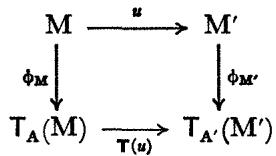
\includegraphics[keepaspectratio]{images/part003_9672ae23.jpg}}

If \(\sigma: \mathbf{A}' \to \mathbf{A}''\) is a commutative ring homomorphism, \(\mathbf{M}''\) an \(\mathbf{A}''\) -module and \(v: \mathbf{M}' \to \mathbf{M}''\) an \(\mathbf{A}'\) -homomorphism, the above uniqueness property shows that

\[
\mathbf {T} (v \circ u) = \mathbf {T} (v) \circ \mathbf {T} (u).\tag{9}
\]

PROPOSITION 5. Let A, B be two commutative rings, \(\rho: \mathbf{A} \to \mathbf{B}\) a ring homomorphism and M an A-module. The canonical extension

\[
\psi : \mathsf {T} _ {\mathbf {B}} (\mathbf {B} \otimes_ {\mathbf {A}} \mathbf {M}) \rightarrow \mathbf {B} \otimes_ {\mathbf {A}} \mathsf {T} _ {\mathbf {A}} (\mathbf {M})
\]

of the B-linear mapping \(\mathbf{1}_{\mathbf{B}} \otimes \phi_{\mathbf{M}}: \mathbf{B} \otimes_{\mathbf{A}} \mathbf{M} \to \mathbf{B} \otimes_{\mathbf{A}} \mathsf{T}_{\mathbf{A}}(\mathbf{M})\) is an isomorphism of graded B-algebras.

Consider the two A-algebra homomorphisms: the canonical injection \(j: \mathbf{B} = \mathsf{T}^0(\mathbf{B} \otimes_{\mathbf{A}} \mathbf{M}) \to \mathsf{T}(\mathbf{B} \otimes_{\mathbf{A}} \mathbf{M})\) and the homomorphism

\[
h = \mathsf {T} (i): \mathsf {T} (\mathbf {M}) \rightarrow \mathsf {T} (\mathbf {B} \otimes_ {\mathbf {A}} \mathbf {M})
\]

derived (cf.~formula (8)) from the canonical A-linear mapping

\[
i: \mathbf {M} \rightarrow \mathbf {B} \otimes_ {\mathbf {A}} \mathbf {M}.
\]

As \(\mathsf{T}^0 (\mathbf{B}\otimes_{\mathbf{A}}\mathbf{M})\) is contained in the centre of \(\mathsf{T}(\mathbf{B}\otimes_{\mathbf{A}}\mathbf{M})\) , Proposition 5 of §4, no. 2 can be applied and an A-algebra homomorphism

\[
\psi^ {\prime}: \mathbf {B} \otimes_ {\mathbf {A}} \mathsf {T} (\mathbf {M}) \rightarrow \mathsf {T} (\mathbf {B} \otimes_ {\mathbf {A}} \mathbf {M})
\]

is obtained such that, for \(\beta \in \mathbf{B}\) , \(x_{i} \in \mathbf{M}\) for \(1 \leqslant i \leqslant n\) ,

\[
\psi^ {\prime} (\beta \otimes (x _ {1} \otimes x _ {2} \otimes \dots \otimes x _ {n})) = \beta ((1 \otimes x _ {1}) \otimes (1 \otimes x _ {2}) \otimes \dots \otimes (1 \otimes x _ {n})),
\]

which shows immediately that \(\psi'\) is also a B-algebra homomorphism. It suffices to prove that \(\psi \circ \psi'\) and \(\psi' \circ \psi\) are the identity mappings on \(B \otimes_{A} T(M)\) and \(T(B \otimes_{A} M)\) respectively. Now, these two algebras are generated by \(B \otimes_{A} M\) and clearly \(\psi \circ \psi'\) and \(\psi' \circ \psi\) coincide with the identity mapping on \(B \otimes_{A} M\) , whence the conclusion.

\subsection{DIRECT LIMIT OF TENSOR ALGEBRAS}

Let \((\mathbf{A}_{\alpha},\phi_{\beta \alpha})\) be a directed direct system of commutative rings and \((\mathbf{M}_{\alpha},f_{\beta \alpha})\) a direct system of \(\mathbf{A}_{\alpha}\) -modules (II, § 6, no. 2); let \(\mathbf{A} = \varinjlim \mathbf{A}_{\alpha}\) and \(\mathbf{M} = \varinjlim \mathbf{M}_{\alpha}\) , which is an A-module. For \(\alpha \leqslant \beta\) an \(\mathbf{A}_{\alpha}\) -algebra homomorphism (no. 3, formula (8)) \(f_{\beta \alpha}' = \mathsf{T}(f_{\beta \alpha})\colon \mathsf{T}_{\mathbf{A}_{\alpha}}(\mathbf{M}_{\alpha})\to \mathsf{T}_{\mathbf{A}_{\beta}}(\mathbf{M}_{\beta})\) is derived canonically from the \(\mathbf{A}_{\alpha}\) -homomorphism \(f_{\beta \alpha}\colon \mathbf{M}_{\alpha}\to \mathbf{M}_{\beta}\) and it follows from (9) (no. 3) that \((\mathsf{T}_{\mathbf{A}_{\alpha}}(\mathbf{M}_{\alpha}),f_{\beta \alpha}')\) is a direct system of \(\mathbf{A}_{\alpha}\) -algebras. On the other hand let \(f_{\alpha}\colon \mathbf{M}_{\alpha}\to \mathbf{M}\) be the canonical \(\mathbf{A}_{\alpha}\) -homomorphism; an \(\mathbf{A}_{\alpha}\) -algebra homomorphism \(f_{\alpha}'\colon \mathsf{T}_{\mathbf{A}_{\alpha}}(\mathbf{M}_{\alpha})\to \mathsf{T}_{\mathbf{A}}(\mathbf{M})\) is derived (no. 3, formula (8)) and it also follows from (9) (no. 3) that the \(f_{\alpha}'\) constitute a direct system of \(\mathbf{A}_{\alpha}\) -homomorphisms.

PROPOSITION 6. The A-homomorphism \(f' = \varinjlim f_{\alpha}' : \varinjlim T_{A_{\alpha}}(M_{\alpha}) \to T_{A}(M)\) is a graded algebra isomorphism.

To simplify we write \(\mathbf{E} = T_{\mathbf{A}}(\mathbf{M})\) and \(\mathbf{E}' = \varinjlim T_{\mathbf{A}_{\alpha}}(\mathbf{M}_{\alpha})\) and let

\[
g _ {\alpha}: \mathsf {T} _ {\mathrm{A} _ {\alpha}} (\mathbf {M} _ {\alpha}) \rightarrow \mathbf {E} ^ {\prime}
\]

be the canonical \(\mathbf{A}_{\alpha}\) -homomorphism. Clearly the composite \(\mathbf{A}_{\alpha}\) -linear mappings \(\mathbf{M}_{\alpha} \xrightarrow{\phi_{\mathbf{M}_{\alpha}}} \mathsf{T}_{\mathbf{A}_{\alpha}}(\mathbf{M}_{\alpha}) \xrightarrow{g_{\alpha}} \mathbf{E}'\) form a direct system and there is therefore one and only one A-linear mapping \(u = \varinjlim (g_{\alpha} \circ \phi_{\mathbf{M}_{\alpha}}): \mathbf{M} \to \mathbf{E}'\) such that

\[
u \circ f _ {\alpha} = g _ {\alpha} \circ \phi_ {M _ {\alpha}}
\]

for all \(\alpha\) . This mapping itself factorizes uniquely (no. 1, Proposition 1) into \(\mathbf{M} \xrightarrow{\phi_{\mathbf{M}}} \mathrm{E} \to \mathrm{E}'\) , where \(h\) is an A-algebra homomorphism. It will suffice to prove that \(h \circ f' = 1_{\mathrm{E}'}\) and \(f' \circ h = 1_{\mathrm{E}}\) .

To this end note that, for every index \(\alpha\) , (no. 3, formula (8))

\[
h \circ f _ {\alpha} ^ {\prime} \circ \phi_ {M _ {\alpha}} = h \circ \phi_ {M} \circ f _ {\alpha} = u \circ f _ {\alpha} = g _ {\alpha} \circ \phi_ {M _ {\alpha}}
\]

whence, by the uniqueness assertion of no. 1, Proposition 1,

\[
h \circ f _ {\alpha} ^ {\prime} = g _ {\alpha}
\]

for all \(\alpha\) ; it follows that \((h \circ f') \circ g_{\alpha} = g_{\alpha}\) for all \(\alpha\) and hence \(h \circ f' = 1_{\mathbf{E}'}\) by definition of a direct limit.

On the other hand, by virtue of no. 3, formula (8),

\[
f ^ {\prime} \circ u \circ f _ {\alpha} = f ^ {\prime} \circ g _ {\alpha} \circ \phi_ {M _ {\alpha}} = f _ {\alpha} ^ {\prime} \circ \phi_ {M _ {\alpha}} = \phi_ {M} \circ f _ {\alpha},
\]

whence again \(f' \circ u = \phi_{\mathbb{M}}\) by definition of a direct limit; we conclude that \(f' \circ h \circ \phi_{\mathbb{M}} = \phi_{\mathbb{M}}\) and the uniqueness property of no. 1, Proposition 1 gives \(f' \circ h = 1_{\mathbb{E}}\) .

Proposition 6 can also be shown by observing that, for every integer \(n \geqslant 1\) , there is a canonical A-module isomorphism \(\lim_{\longrightarrow} \mathsf{T}_{\mathbf{A}_{\alpha}}^{n}(\mathbf{M}_{\alpha}) \to \mathsf{T}_{\mathbf{A}}^{n}(\mathbf{M})\) , as follows by induction on \(n\) from II, § 6, no. 3, Proposition 7. It is immediately verified that these isomorphisms are the restrictions of \(f'\) .

\subsection{TENSOR ALGEBRA OF A DIRECT SUM. TENSOR ALGEBRA OF A FREE MODULE. TENSOR ALGEBRA OF A GRADED MODULE}

Let A be a commutative ring and \(M = \bigoplus_{\lambda \in L} M_{\lambda}\) the direct sum of a family of A-modules. It follows from II, §3, no. 7, Proposition 7, by induction on n, that \(T^{n}(M)\) is the direct sum of the submodules the images of the canonical injections

\[
\mathbf {M} _ {\lambda_ {1}} \otimes \mathbf {M} _ {\lambda_ {2}} \otimes \dots \otimes \mathbf {M} _ {\lambda_ {n}} \rightarrow \mathsf {T} ^ {n} (\mathbf {M}) = \mathbf {M} ^ {\otimes n}
\]

relative to all the sequences \((\lambda_{i})\in\mathbf{L}^{n}\) . Identifying \(M_{\lambda_{1}}\otimes M_{\lambda_{2}}\otimes\cdots\otimes M_{\lambda_{n}}\) with this image, it is seen that \(T(\mathbf{M})\) is the direct sum of all the modules

\[
\mathbf {M} _ {\lambda_ {1}} \otimes \mathbf {M} _ {\lambda_ {2}} \otimes \dots \otimes \mathbf {M} _ {\lambda_ {n}}
\]

where \(n\) runs through \(\mathbf{N}\) and, for each \(n\) , \((\lambda_t)\) runs through \(\mathbf{L}^n\) .

We first deduce the following consequence:

THEOREM 1. Let A be a commutative ring, M a free A-module and \((e_{\lambda})_{\lambda \in L}\) a basis of M. Then the elements \(e_{s} = e_{\lambda_{1}} \otimes e_{\lambda_{2}} \otimes \cdots \otimes e_{\lambda_{n}}\) , where \(s = (\lambda_{1}, \ldots, \lambda_{n})\) runs through the set of all finite sequences of elements of L and \(e_{\varnothing}\) is used to denote the unit element of T(M), form a basis of the A-module T(M).

The elements of this basis are obviously homogeneous and the multiplication table is given by

\[
e _ {s} e _ {t} = e _ {s t}\tag{10}
\]

where \(st\) denotes the sequence of elements of \(\mathbf{L}\) obtained by juxtaposing the sequences \(s\) and \(t\) (I, § 7, no. 2).

It is seen that the basis \((e_{s})\) of T(M), with the multiplicative law (10), is canonically isomorphic to the free monoid of the set L (I, §7, no. 2), the isomorphism being obtained by mapping each word s of this monoid to the element \(e_{s}\) . It follows (§2, no. 7) that the tensor algebra T(M) of a free module M, with a basis of indexing set L, is canonically isomorphic to the free associative algebra of L over A. In particular (§2, no. 7, Proposition 7), for every mapping \(f: L \to E\) from L to an A-algebra E, there exists one and only one A-algebra homomorphism \(\bar{f}: T(M) \to E\) such that \(\bar{f}(e_{\lambda}) = f(\lambda)\) .

Remark. The above results can equally be obtained as a consequence of the universal properties of the free associative algebra and of the tensor algebra, using II, § 3, no. 7, Corollary 2 to Proposition 7.

COROLLARY. If M is a projective A-module, T(M) is a projective A-module.

M is a direct factor of a free A-module N (II, §2, no. 2, Proposition 4) and hence T(M) is a direct factor of T(N) (no. 2); as T(N) is free (Theorem 1), this shows that T(M) is projective (II, §2, no. 2).

PROPOSITION 7. Let \(\Delta\) be a commutative monoid, \(\mathbf{M}\) a graded A-module of type \(\Delta\) and \((\mathbf{M}_{\alpha})_{\alpha \in \Delta}\) its graduation. For every ordered pair \((\alpha, n) \in \Delta \times \mathbf{N}\) , let \(\mathsf{T}^{\alpha,n}(\mathbf{M})\) be the (direct) sum of the submodules \(\mathbf{M}_{\alpha_1} \otimes \mathbf{M}_{\alpha_2} \otimes \dots \otimes \mathbf{M}_{\alpha_n}\) of \(\mathsf{T}^n(\mathbf{M})\) such that \(\sum_{i=1}^{n} \alpha_i = \alpha\) ; then \((T^{\alpha, n}(M))_{(\alpha, n) \in \Delta \times N}\) is the only graduation of type \(\Delta \times N\) compatible with the algebra structure on \(T(M)\) and inducing on \(M = T^1(M)\) the given graduation.

It has been seen at the beginning of this no. that \(\mathsf{T}(\mathbf{M})\) is the direct sum of the \(\mathsf{T}^{\alpha,n}(\mathbf{M})\) and the fact that this is a graduation compatible with the algebra structure follows immediately from the definitions. If \((\mathsf{T}'^{\alpha,n})\) is another graduation of type \(\Delta \times \mathbf{N}\) on \(\mathsf{T}(\mathbf{M})\) compatible with the algebra structure and such that \(\mathsf{T}^{\alpha,1}(\mathbf{M}) = \mathsf{T}'^{\alpha,1}\) for \(\alpha \in \Delta\) , it follows immediately from the definitions that, for all \(n \geqslant 1\) and all \(\alpha \in \Delta\) , \(\mathsf{T}^{\alpha,n}(\mathbf{M}) \subset \mathsf{T}'^{\alpha,n}\) ; but since \(\mathsf{T}(\mathbf{M})\) is also the direct sum of the \(\mathsf{T}^{\alpha,n}(\mathbf{M})\) , this implies that \(\mathsf{T}'^{\alpha,n} = \mathsf{T}^{\alpha,n}(\mathbf{M})\) (II, § 1, no. 8, Remark).

\subsection{TENSORS AND TENSOR NOTATION}

Let A be a commutative ring, M an A-module, \(\mathbf{M}^*\) the dual of M (II, § 2, no. 3) and I and J two disjoint finite sets; the A-module \(\bigotimes_{i\in \mathrm{I}\cup \mathrm{J}}\mathbf{E}_i\) , where \(\mathbf{E}_i = \mathbf{M}\) if \(i\in \mathrm{I}\) , \(\mathbf{E}_i = \mathbf{M}^*\) if \(i\in \mathrm{J}\) , is denoted by \(\mathsf{T}_{\mathsf{J}}^{\mathsf{I}}(\mathbf{M})\) ; the elements of \(\mathsf{T}_{\mathsf{J}}^{\mathsf{I}}(\mathbf{M})\) are called tensors of type (I,J) over M. They are called contravariant if \(\mathbf{J} = \varnothing\) , covariant if \(\mathbf{I} = \varnothing\) and mixed otherwise.

Let \(I'\) , \(I''\) be two subsets of I and \(J'\) , \(J''\) two subsets of J such that \(I' \cup I'' = I\) , \(\mathbf{I}' \cap \mathbf{I}'' = \varnothing, \mathbf{J}' \cup \mathbf{J}'' = \mathbf{J}, \mathbf{J}' \cap \mathbf{J}'' = \varnothing\) ; then there is a canonical associativity isomorphism (II, § 3, no. 9)

\[
\mathsf {T} _ {\mathbf {J}} ^ {\mathbf {I}} (\mathbf {M}) \rightarrow \mathsf {T} _ {\mathbf {J} ^ {\prime}} ^ {\mathbf {I} ^ {\prime}} (\mathbf {M}) \otimes_ {\mathbf {A}} \mathsf {T} _ {\mathbf {J} ^ {\prime \prime}} ^ {\mathbf {I} ^ {\prime \prime}} (\mathbf {M}).\tag{11}
\]

Considering the tensor algebra \(\mathsf{T}(\mathbf{M}\oplus \mathbf{M}^{*})\) , it follows from no. 5 that \(\mathsf{T}^n (\mathbf{M}\oplus \mathbf{M}^*)\) is canonically identified with the direct sum of the \(\mathsf{T}_{\mathbf{J}}^{\mathbf{I}}(\mathbf{M})\) where I runs through the set of subsets of the interval \([1,n]\) of \(\mathbf{N}\) and J is the complement of I in \([1,n]\) .

When \(I = [1, p]\) and \(J = [p + 1, p + q]\) with integers \(p \geqslant 0\) , \(q \geqslant 0\) (where we replace I (resp. J) by \(\varnothing\) when \(p = 0\) (resp. \(q = 0\) )), the A-module \(T_J^I(M)\) is also denoted by \(T_q^p(M)\) ; the A-modules \(T_0^n(M)\) and \(T_n^0(M)\) are therefore by definition the A-modules \(T^n(M)\) and \(T^n(M^*)\) respectively. When I and J are arbitrary finite sets of cardinals \(p = \text{Card}(I)\) and \(q = \text{Card}(J)\) , we give each of them a total ordering; then there exists an increasing bijection of I (resp. J) onto \([1, p]\) (resp. \([p + 1, p + q]\) ) and these bijections therefore define an isomorphism

\[
\mathbf {T} _ {\mathrm{J}} ^ {\mathrm{I}} (\mathbf {M}) \rightarrow \mathbf {T} _ {q} ^ {p} (\mathbf {M}).
\]

When M is a finitely generated projective A-module, it follows from II, § 2, no. 7, Corollary 4 to Proposition 13 and II, § 4, no. 4, Corollary 1 to Proposition 4 that there is a canonical isomorphism

\[
(\mathsf {T} _ {\mathbf {J}} ^ {\mathbf {I}} (\mathbf {M})) ^ {*} \to \mathsf {T} _ {\mathbf {I}} ^ {\mathbf {J}} (\mathbf {M}).
\]

Suppose now that \(\mathbf{M}\) is a finitely generated free A-module and let \((e_{\lambda})_{\lambda \in L}\) be a basis of \(\mathbf{M}\) (L therefore being a finite set). The basis of \(\mathbf{M}^*\) dual to \((e_{\lambda})\) (II, §2, no. 6) is denoted by \((e^{\lambda})_{\lambda \in L}\) . The bases \((e_{\lambda})\) and \((e^{\lambda})\) of \(\mathbf{M}\) and \(\mathbf{M}^*\) respectively define (no. 5) a basis of \(\mathsf{T}_{\mathbf{J}}^{\mathbf{I}}(\mathbf{M})\) , which we give explicitly as follows: given two mappings \(f\colon \mathbf{I} \to \mathbf{L}\) and \(g\colon \mathbf{J} \to \mathbf{L}\) , let \(e_f^g\) be the element \(\bigotimes_{i \in I \cup J} x_i\) of \(\mathsf{T}_{\mathbf{J}}^{\mathbf{I}}(\mathbf{M})\) defined by

\[
x _ {i} = e _ {f (i)} \quad \text { if } i \in \mathbf {I}, \qquad x _ {i} = e ^ {g (i)} \quad \text { if } i \in \mathbf {J}.
\]

When \((f, g)\) runs through the set of ordered pairs of mappings \(f: \mathbf{I} \to \mathbf{L}\) and \(g: \mathbf{J} \to \mathbf{L}\) , the \(e_f^g\) form a basis of the A-module \(\mathsf{T}_{\mathbf{J}}^{\mathbf{I}}(\mathbf{M})\) , said to be associated with the given basis \((e_{\lambda})\) of \(\mathbf{M}\) . For \(z \in \mathsf{T}_{\mathbf{J}}^{\mathbf{I}}(\mathbf{M})\) , we can therefore write

\[
z = \sum_ {(f, g)} \alpha_ {g} ^ {f} (z). e _ {f} ^ {g}\tag{12}
\]

where the \(\alpha_g^f\) are the coordinate forms relative to the basis \((e_f^g)\) ; by an abuse of language, the \(\alpha_g^f(z)\) are called the coordinates of the tensor \(z\) with respect to the basis \((e_\lambda)\) of the module M. The \(\alpha_g^f\) constitute the dual basis of \((e_g^f)\) , in other words they are identified with the elements of the basis of \(\mathsf{T}_{\mathbf{I}}^{\mathbf{j}}(\mathbf{M})\) , associated with \((e_\lambda)\) . When I and J are complementary subsets of an interval \([1,n]\) of N, \(\alpha_g^f\) (or \(\alpha_g^f(z)\) ) is denoted as follows: each element \(f(i)\) for \(i\in I\) is written as an upper index in the \(i\) -th place with a dot in the \(i\) -th place for \(i \in \mathbf{J}\) ; similarly, \(g(i)\) for \(i \in \mathbf{J}\) is written as a lower index in the \(i\) -th place with a dot in the \(i\) -th place for \(i \in \mathbf{I}\) . For example, for \(\mathbf{I} = \{1, 4\}\) , \(\mathbf{J} = \{2, 3\}\) , we write \(\alpha_{\cdot \nu \rho}^{\lambda \cdot \cdot \mu}\) if \(f(1) = \lambda, f(4) = \mu, g(2) = \nu, g(3) = \rho\) .

Let \((\bar{e}_{\lambda})_{\lambda \in L}\) be another basis of M and \(P\) the matrix of passing from \((e_{\lambda})\) to \((\bar{e}_{\lambda})\) (II, § 10, no. 8). Then the matrix of passing from \((e^{\lambda})\) to \((\bar{e}^{\lambda})\) (dual basis of \((\bar{e}_{\lambda}))\) is the contragredient \(^{t}P^{-1}\) of \(P\) (II, § 10, no. 8, Proposition 5). It follows (II, § 10, no. 10) that the matrix of passing from the basis \((e_{f}^{g})\) of \(\mathrm{T}_{\mathrm{J}}^{\mathrm{I}}(\mathrm{M})\) to the basis \((\bar{e}_{f}^{g})\) (where \(f\) (resp. \(g\) ) runs through the set of mappings of I into L (resp. of J into L)) is the matrix

\[
\bigotimes_ {i \in I \cup J} Q _ {i}, \quad \text { where } Q _ {i} = P \text { if } i \in I, Q _ {i} = ^ {t} P ^ {- 1} \text { if } i \in J.\tag{13}
\]

The transpose of this matrix is therefore identified with

\[
\bigotimes_ {i \in \mathbf {I} \cup J} R _ {i}, \quad \text { where } R _ {i} = ^ {t} P ^ {- 1} \text { if } i \in \mathbf {I}, R _ {i} = P \text { if } i \in \mathbf {J}.\tag{14}
\]

Suppose now that \(\mathbf{M}\) is an arbitrary module. Let \(i\in \mathbf{I}, j\in \mathbf{J}\) and write \(\mathbf{I}' = \mathbf{I} - \{i\}, J' = J - \{j\}\) ; we shall define a canonical A-linear mapping

\[
c _ {j} ^ {i} \colon \mathsf {T} _ {\mathbf {J}} ^ {\mathbf {I}} (\mathbf {M}) \to \mathsf {T} _ {\mathbf {J} ^ {\prime}} ^ {\mathbf {I} ^ {\prime}} (\mathbf {M}),
\]

called contraction of the index \(i\) and the index \(j\) . For this, note that the mapping of \(\mathbf{M}^{\mathrm{I}} \times (\mathbf{M}^{*})^{\mathrm{J}}\) , which associates with every family \((x_{i})_{i \in \mathbf{I} \cup \mathbf{J}}\) , where \(x_{i} \in \mathbf{M}\) if \(i \in \mathbf{I}\) and \(x_{i} \in \mathbf{M}^{*}\) if \(i \in \mathbf{J}\) , the element

\[
\left\langle x _ {i}, x _ {j} \right\rangle \otimes_ {k \in (\mathbb {I} \cup \mathbb {J}) - \{i, j \}} x _ {k}\tag{15}
\]

of \(T_{J'}^{I'}(M)\) , is A-multilinear; \(c_{j}^{i}\) is the corresponding A-linear mapping.

Suppose now that M is free and finitely generated and let \((e_{\lambda})_{\lambda \in L}\) be a basis of M. Given two mappings \(f: I \to L\) , \(g: J \to L\) , let \(f_i\) denote the restriction of f to \(I' = I - \{i\}\) and \(g_j\) the restriction of g to \(J' = J - \{j\}\) ; then by virtue of (12)

\[
c _ {j} ^ {i} (e _ {f} ^ {g}) = \left\{ \begin{array}{l l} 0 & \text { if } f (i) \neq g (j) \\ e _ {f _ {i}} ^ {g _ {j}} & \text { if } f (i) = g (j) \end{array} \right.\tag{16}
\]

The expression for the coordinates of \(c_j^i(z)\) as a function of those of \(z\) is obtained; for every mapping \(f'\) (resp. \(g'\) ) of \(I'\) into \(L\) (resp. of \(J'\) into \(L\) ) and every \(\lambda \in L\) , let \((f', \lambda)\) (resp. \((g', \lambda)\) ) denote the mapping of \(I\) into \(L\) (resp. of \(J\) into \(L\) ) whose restriction to \(I'\) (resp. \(J'\) ) is \(f'\) (resp. \(g'\) ) and which takes the value \(\lambda\) at the element \(i\) (resp. \(j\) ). Then, if the coordinate forms relative to the basis \((e_{f'}^{g'})\) of \(T_{J'}^{I'}(M)\) are denoted by \(\beta_{g'}^{f'}\) ,

\[
\beta_ {g ^ {\prime}} ^ {f ^ {\prime}} (c _ {j} ^ {i} (z)) = \sum_ {\lambda \in L} \alpha_ {(g ^ {\prime}, \lambda)} ^ {(f ^ {\prime}, \lambda)} (z).\tag{17}
\]

Examples of tensors. (1) Let M be a finitely generated projective A-module. We know (II, § 4, no. 2, Corollary to Proposition 2), that there is a canonical A-module isomorphism

\[
\theta_ {\mathbf {M}} \colon \mathbf {M} ^ {*} \otimes_ {\mathbf {A}} \mathbf {M} \rightarrow \operatorname{End} _ {\mathbf {A}} (\mathbf {M})
\]

such that \(\theta_{\mathbf{M}}(x^{*}\otimes x)\) (for \(x\in \mathbf{M},x^{*}\in \mathbf{M}^{*}\) ) is the endomorphism

\[
y \mapsto \langle y, x ^ {*} \rangle x.
\]

Hence, by means of \(\theta_{\mathbf{M}}\) , \(\mathsf{T}_{(1)}^{(2)}(\mathbf{M})\) (isomorphic to \(\mathsf{T}_1^1 (\mathbf{M}))\) can be identified with the A-module \(\operatorname{End}_{\mathbf{A}}(\mathbf{M})\) . Suppose that \(\mathbf{M}\) is a free module and let \((e_{\lambda})_{\lambda \in \mathbf{L}}\) be a basis of \(\mathbf{M}\) ; then the coordinates of a tensor \(z\in \mathbf{M}^*\otimes \mathbf{M}\) relative to the basis \((e^{\mu}\otimes e_{\lambda})\) of this module are denoted by \(\zeta_{\mu}^{\cdot \lambda}\) . As \(\theta_{\mathrm{M}}(e^{\mu}\otimes e_{\lambda})\) is the endomorphism \(y\mapsto \langle y,e^{\mu}\rangle e_{\lambda}\) , the endomorphism \(u = \theta_{\mathrm{M}}(z) = \theta_{\mathrm{M}}\left(\sum_{\lambda ,\mu}\zeta_{\mu}^{\cdot \lambda}e^{\mu}\otimes e_{\lambda}\right)\) maps \(y\) to \(\sum_{\lambda ,\mu}\zeta_{\mu}^{\cdot \lambda}\langle y,e^{\mu}\rangle e_{\lambda}\) ; writing \(y = e_{\lambda}\) , we obtain the relation

\[
u (e _ {\lambda}) = \sum_ {\mu \in L} \zeta_ {\lambda} ^ {\cdot \mu} e _ {\mu}\tag{18}
\]

in other words, the matrix of the linear mapping \(u = \theta_{\mathrm{M}}(z)\) is that whose element in the row of index \(\mu\) and column of index \(\lambda\) is \(\zeta_{\lambda}^{\mu}\) .

The definition of the trace of \(u\) (II, § 4, no. 3) shows immediately that

\[
\operatorname{Tr} (\theta_ {\mathbb {M}} (z)) = c _ {1} ^ {2} (z).
\]

Therefore the element \(z_0 = \sum_{\lambda \in L} e^\lambda \otimes e_\lambda\) (whose coordinates \(\zeta_\mu^{\cdot \lambda}\) are zero for \(\lambda \neq \mu\) and equal to 1 for \(\lambda = \mu\) ), which is such that \(\theta_M(z_0) = 1_M\) , is the image of the element \(1 \in A = T_0^0(M)\) under the mapping the transpose of the contraction

\[
c _ {1} ^ {2}: \mathbf {T} _ {\{1 \}} ^ {\{2 \}} (\mathbf {M}) \rightarrow \mathbf {A}.
\]

\begin{enumerate}
\def\labelenumi{(\arabic{enumi})}
\setcounter{enumi}{1}
\tightlist
\item
  Suppose always that M is a finitely generated projective A-module; there is a canonical A-module isomorphism
\end{enumerate}

\[
\mu : \mathbf {M} ^ {*} \otimes_ {\mathbf {A}} \mathbf {M} ^ {*} \rightarrow (\mathbf {M} \otimes_ {\mathbf {A}} \mathbf {M}) ^ {*}
\]

(II, § 4, no. 4, Corollary 1 to Proposition 2) and a canonical isomorphism

\[
\theta : (\mathbf {M} \otimes_ {\mathbf {A}} \mathbf {M}) ^ {*} \otimes_ {\mathbf {A}} \mathbf {M} \rightarrow \operatorname{Hom} _ {\mathbf {A}} (\mathbf {M} \otimes_ {\mathbf {A}} \mathbf {M}, \mathbf {M})
\]

(II, §4, no. 2, Corollary to Proposition 2); also \(\operatorname{Hom}_{\mathbf{A}}(\mathbf{M} \otimes_{\mathbf{A}} \mathbf{M}, \mathbf{M})\) is canonically isomorphic to the A-module \(\mathcal{L}_2(\mathbf{M}, \mathbf{M}; \mathbf{M})\) of A-bilinear mappings of \(\mathbf{M} \times \mathbf{M}\) into \(\mathbf{M}\) (II, §3, no. 9). Composing these isomorphisms, a canonical isomorphism is obtained

\[
\chi_ {\mathbf {M}} \colon T _ {\{1, 2 \}} ^ {(3)} (\mathbf {M}) = \mathbf {M} ^ {*} \otimes \mathbf {M} ^ {*} \otimes \mathbf {M} \rightarrow \mathcal {L} _ {2} (\mathbf {M}, \mathbf {M}; \mathbf {M})
\]

such that, for \(x^{*}, y^{*}\) in \(\mathbf{M}^{*}\) , \(z \in \mathbf{M}\) , \(\chi_{\mathbf{M}}(x^{*} \otimes y^{*} \otimes z)\) is the bilinear mapping

\[
(u, v) \mapsto \langle u, x ^ {*} \rangle \langle v, y ^ {*} \rangle z.
\]

Hence, by means of \(\chi_{\mathbf{M}}\) , \(\mathsf{T}_{\{1,2\}}^{(3)}(\mathbf{M})\) (isomorphic to \(\mathsf{T}_{2}^{1}(\mathbf{M})\) ) can be identified with the A-module \(\mathcal{L}_2(\mathbf{M},\mathbf{M};\mathbf{M})\) . Suppose that \(\mathbf{M}\) is a free A-module and let \((e_{\lambda})_{\lambda \in L}\) be a basis of \(\mathbf{M}\) ; then the coordinates of a tensor \(z\in \mathbf{M}^*\otimes \mathbf{M}^*\otimes \mathbf{M}\) relative to the basis \((e^{\lambda}\otimes e^{\mu}\otimes e_{\nu})\) of this module are denoted by \(\zeta_{\lambda \mu}^{\cdot \cdot \nu}\) . The bilinear mapping \(\chi_{\mathbf{M}}(z)\) maps the ordered pair \((e_{\lambda},e_{\mu})\) to

\[
\sum_ {\nu \in L} \zeta_ {\lambda \mu}^{\cdot \cdot \nu} e _ {\nu}
\]

and therefore the \(\zeta_{\lambda \mu}^{\cdots \nu}\) are just the constants of structure of the (in general non-associative) algebra defined on \(\mathbf{M}\) by the bilinear mapping \(\chi_{\mathbf{M}}(z)\) , with respect to the basis \((e_{\lambda})\) ( \(\S 1\) , no. 7).

Remark 2. Let \((e_{\lambda})_{\lambda \in L}, (\tilde{e}_{\lambda})_{\lambda \in L}\) be two bases of M and \(P\) the matrix of passage from \((e_{\lambda})\) to \((\tilde{e}_{\lambda})\) . On account of what was seen in Example 1, the element of \(P\) appearing in the row of index \(\lambda\) and the column of index \(\mu\) is denoted by \(\alpha_{\mu}^{\lambda}\) and the element of the contragredient \(^{t}P^{-1}\) appearing in the row of index \(\lambda\) and the column of index \(\mu\) is denoted by \(\beta_{\lambda}^{\mu}\) . Then (in the notation introduced above)

\begin{enumerate}
\def\labelenumi{(\arabic{enumi})}
\setcounter{enumi}{18}
\tightlist
\item
\end{enumerate}

\[
\left\{ \begin{array}{l} \tilde {e} _ {\mu} = \sum_ {\lambda} \alpha_ {\mu} ^ {\lambda} e _ {\lambda} \\ \tilde {e} ^ {\mu} = \sum_ {\lambda} \beta_ {\lambda} ^ {\mu} e ^ {\lambda} \end{array} \right.\tag{20}
\]

\[
\bar {e} _ {f ^ {\prime}} ^ {g ^ {\prime}} = \sum_ {(f, g)} \left(\prod_ {i \in I} \alpha_ {f ^ {\prime} (i)} ^ {f (i)}\right) \left(\prod_ {j \in J} \beta_ {g (j)} ^ {g ^ {\prime} (j)}\right) e _ {f} ^ {g}
\]

for all mappings \(f': \mathbf{I} \to \mathbf{L}\) and \(g': \mathbf{J} \to \mathbf{L}\) . The coordinates \(\zeta_g^f\) of a tensor \(z \in \mathbb{T}_J^{\mathbf{I}}(\mathbf{M})\) with respect to the basis \((e_{\lambda})\) can therefore be expressed in terms of the coordinates \(\bar{\zeta}_{g'}^{f'}\) of \(z\) with respect to the basis \((\bar{e}_{\lambda})\) using the formulae

\[
\zeta_ {g} ^ {f} = \sum_ {(f ^ {\prime}, g ^ {\prime})} \left(\prod_ {i \in I} \alpha_ {f ^ {\prime} (i)} ^ {f (i)}\right) \left(\prod_ {j \in J} \beta_ {g (j)} ^ {g ^ {\prime} (j)}\right) \bar {\zeta} _ {g ^ {\prime}} ^ {f ^ {\prime}}.\tag{21}
\]

The matrix \(P^{-1}\) of passage from the basis \((\tilde{e}_{\lambda})\) to the basis \((e_{\lambda})\) is the transpose of \(^{t}P^{-1}\) , so that \(\beta_{\lambda}^{\mu}\) is the element which appears in the column of index \(\lambda\) and the row of index \(\mu\) of \(P^{-1}\) . The calculation of \(e_{f}^{g}\) in terms of the \(\tilde{e}_{f'}^{g'}\) and that of the \(\overline{\zeta}_{g'}^{f'}\) in terms of the \(\zeta_{g}^{f}\) are therefore made by replacing \(\alpha_{\mu}^{\lambda}\) by \(\beta_{\lambda}^{\mu}\) and \(\beta_{\lambda}^{\mu}\) by \(\alpha_{\mu}^{\lambda}\) in the above calculations and exchanging the roles of \(f\) and \(f'\) and those of \(g\) and \(g'\) . Then

\[
e _ {f} ^ {g} = \sum_ {(f ^ {\prime}, g ^ {\prime})} \left(\prod_ {j \in J} \alpha_ {g ^ {\prime} (j)} ^ {g (j)}\right) \left(\prod_ {i \in I} \beta_ {f (i)} ^ {f ^ {\prime} (i)}\right) \bar {e} _ {f ^ {\prime}} ^ {g ^ {\prime}}\tag{22}
\]

\[
\bar {\zeta} _ {g ^ {\prime}} ^ {f ^ {\prime}} = \sum_ {(f, g)} \left(\prod_ {j \in J} \alpha_ {g ^ {\prime} (j)} ^ {g (j)}\right) \left(\prod_ {i \in I} \beta_ {f (i)} ^ {f ^ {\prime} (i)}\right) \zeta_ {g} ^ {f}.\tag{23}
\]

The above formulae are such that the summation is over indices which appear once as a lower index and once as an upper index. Certain authors allow themselves because of this circumstance to suppress the summation signs.

\section{SYMMETRIC ALGEBRAS}

\subsection{DEFINITION OF THE SYMMETRIC ALGEBRA OF A MODULE}

DEFINITION 1. Let A be a commutative ring and M an A-module. The symmetric algebra of M, denoted by S(M), or Sym(M), or \(S_{A}(M)\), is the quotient algebra over A of the tensor algebra T(M) by the two-sided ideal \(\mathfrak{J}'\) (also denoted by \(\mathfrak{J}_{\mathbf{M}}'\) ) generated by the elements \(xy - yx = x \otimes y - y \otimes x\) of T(M), where \(x\) and \(y\) run through M.

Since the ideal \(\mathfrak{J}'\) is generated by homogeneous elements of degree 2, it is a graded ideal (II, §11, no. 3, Proposition 2); we write \(\mathfrak{J}_n' = \mathfrak{J}' \cap T^n(M)\) ; the algebra \(S(M)\) is then graded by the graduation (called canonical) consisting of the \(S^n(M) = T^n(M)/\mathfrak{J}_n'\) . Now \(\mathfrak{J}_0' = \mathfrak{J}_1' = \{0\}\) and hence \(S^0(M)\) is canonically identified with A and \(S^1(M)\) with \(T^1(M) = M\) ; we shall always make these identifications in what follows and denote by \(\phi'\) or \(\phi_M'\) the canonical injection \(M \to S(M)\) .

PROPOSITION 1. The algebra \(\mathbf{S}(\mathbf{M})\) is commutative.

By definition \(\phi'(x)\phi'(y) = \phi'(y)\phi'(x)\) for \(x, y\) in \(\mathbf{M}\) and, as the elements \(\phi'(x)\) , where \(x\) runs through \(\mathbf{M}\) , generate \(\mathbf{S}(\mathbf{M})\) , the conclusion follows from §1, no. 7.

PROPOSITION 2. Let E be an A-algebra and f: M → E an A-linear mapping such that

\[
f (x) f (y) = f (y) f (x) \text {   for   all   } x, y \text {   in   } \mathbf {M}.\tag{1}
\]

There exists one and only one A-algebra homomorphism \(g \colon \mathbb{S}(\mathbf{M}) \to \mathbf{E}\) such that \(f = g \circ \phi'\) .

In other words, \((\mathbb{S}(\mathbf{M}), \phi')\) is a solution of the universal mapping problem (Set Theory, IV, §3, no. 1), where \(\Sigma\) is the species of A-algebra structure, the \(\alpha\) -mappings being the linear mappings of the A-module M to an A-algebra satisfying (1).

The uniqueness of \(g\) follows from the fact that \(\phi'(\mathbf{M}) = \mathbf{M}\) generates \(\mathbf{S}(\mathbf{M})\) . To prove the existence of \(g\) , note that by virtue of § 5, no.~1, Proposition 1 there exists an A-algebra homomorphism \(g_1: \mathbf{T}(\mathbf{M}) \to \mathbf{E}\) such that \(f = g_1 \circ \phi\) ;

all that needs to be proved is that \(g_1\) is zero on the ideal \(\mathfrak{J}'\) , for then, if \(p: \mathsf{T}(\mathbf{M}) \to \mathsf{S}(\mathbf{M}) = \mathsf{T}(\mathbf{M}) / \mathfrak{J}'\) is the canonical homomorphism, we can write \(g_1 = g \circ p\) , where \(g: \mathsf{S}(\mathbf{M}) \to \mathbf{E}\) is an algebra homomorphism, and the conclusion will follow from the fact that \(p \circ \phi = \phi'\) . Now the kernel of \(g_1\) is a two-sided ideal which, by virtue of (1) and the relation \(g_1 \circ \phi = f\) , contains the elements \(x \otimes y - y \otimes x\) for \(x, y\) in \(\mathbf{M}\) . This completes the proof.

Remarks. (1) Suppose that E is a graded A-algebra of type Z, with graduation \((\mathrm{E}_{n})\) , and suppose also that the linear mapping f (assumed to satisfy (1)) is such that

\[
f (\mathbf {M}) \subset \mathrm{E} _ {1}.\tag{2}
\]

Then the relation \(g(x_1x_2 \ldots x_p) = f(x_1)f(x_2) \ldots f(x_p)\) with the \(x_i \in \mathbf{M}\) shows that \(g(\mathbf{S}^p(\mathbf{M})) \subset \mathrm{E}_p\) for all \(p \geqslant 0\) and hence \(g\) is a graded algebra homomorphism.

\begin{enumerate}
\def\labelenumi{(\arabic{enumi})}
\setcounter{enumi}{1}
\item
  Every element of \(\mathsf{S}(\mathbf{M})\) is a sum of products of the form \(x_{1}x_{2}\ldots x_{n}\) , where the \(x_{i}\) belong to \(\mathbf{M}\) ; care should be taken not to confuse such products taken in \(\mathsf{S}(\mathbf{M})\) with the analogous products taken in \(\mathsf{T}(\mathbf{M})\) .
\item
  If \(n!\) .1 is invertible in A, the A-module \(S^n(M)\) is generated by the elements of the form \(x^n\) , where \(x \in M\) ; this follows from the above remark and I, § 8, no. 2, Proposition 2.
\end{enumerate}

\subsection{FUNCTORIAL PROPERTIES OF THE SYMMETRIC ALGEBRA}

PROPOSITION 3. Let A be a commutative ring, M and N two A-modules and u: M → N an A-linear mapping. There exists one and only one A-algebra homomorphism \(u'\) : S(M) → S(N) such that the diagram

\pandocbounded{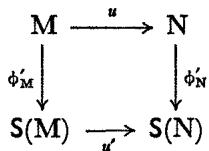
\includegraphics[keepaspectratio]{images/part003_0f38c769.jpg}}

is commutative. Moreover, \(u'\) is a graded algebra homomorphism.

The existence and uniqueness of \(u'\) follow from no. 1, Proposition 2 applied to the commutative algebra \(\mathbf{S}(\mathbf{N})\) and \(f = \phi_{\mathbf{N}}' \circ u: \mathbf{M} \to \mathbf{S}(\mathbf{N})\) ; as

\[
f (\mathbf {M}) \subset \mathbf {S} ^ {1} (\mathbf {N}) = \mathbf {N},
\]

the fact that \(u'\) is a graded algebra homomorphism follows from no. 1, Remark 1.

The homomorphism \(u'\) of Proposition 3 will henceforth be denoted by \(S(u)\) . If \(P\) is an A-module and \(v: N \to P\) an A-linear mapping, then

\[
\mathbf {S} (v \circ u) = \mathbf {S} (v) \circ \mathbf {S} (u)\tag{3}
\]

for \(\mathbf{S}(v) \circ \mathbf{S}(u)\) is an algebra homomorphism rendering commutative the diagram

\pandocbounded{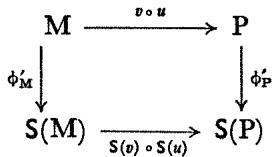
\includegraphics[keepaspectratio]{images/part003_67e6d402.jpg}}

As \(\mathbf{S}(\mathbf{M})\) contains \(\mathbf{M} = \mathbf{S}^1 (\mathbf{M})\) , \(\mathbf{S}(u)\) is sometimes called the canonical extension of \(u\) to \(\mathbf{S}(\mathbf{M})\) . The restriction \(\mathbf{S}^n (u): \mathbf{S}^n (\mathbf{M}) \to \mathbf{S}^n (\mathbf{N})\) is such that

\[
\mathsf {S} ^ {n} (u) \left(x _ {1} x _ {2} \dots x _ {n}\right) = u \left(x _ {1}\right) u \left(x _ {2}\right) \dots u \left(x _ {n}\right)
\]

where the \(x_{i} \in M\) , since \(\mathbf{S}(u)\) is an algebra homomorphism and \(\mathbf{S}^{1}(u) = u\) ; the restriction \(\mathbf{S}^{0}(u)\) to A is the identity mapping. Note that \(\mathbf{S}^{n}(u)\) can be obtained from \(\mathbf{T}^{n}(u): \mathbf{T}^{n}(\mathbf{M}) \to \mathbf{T}^{n}(\mathbf{N})\) by passing to the quotients.

PROPOSITION 4. If \(u: \mathbf{M} \to \mathbf{N}\) is a surjective A-linear mapping, the homomorphism \(\mathbf{S}(u): \mathbf{S}(\mathbf{M}) \to \mathbf{S}(\mathbf{N})\) is surjective and its kernel is the ideal of \(\mathbf{S}(\mathbf{M})\) generated by the kernel \(\mathbf{P} \subset \mathbf{M} \subset \mathbf{S}(\mathbf{M})\) of \(u\) .

We write \(v = \mathsf{T}(u) \colon \mathsf{T}(\mathbf{M}) \to \mathsf{T}(\mathbf{N})\) ; we know (§ 5, no. 2, Proposition 3) that \(v\) is surjective and hence it follows from the definitions that \(v(\mathfrak{J}_{\mathbf{M}}') = \mathfrak{J}_{\mathbf{N}}'\) ; if \(\Re\) is the kernel of \(v\) , then \(v^{-1}(\mathfrak{J}_{\mathbf{N}}') = \Re + \mathfrak{J}_{\mathbf{M}}'\) . As \(\mathsf{S}(u) \colon \mathsf{T}(\mathbf{M}) / \mathfrak{J}_{\mathbf{M}}' \to \mathsf{T}(\mathbf{N}) / \mathfrak{J}_{\mathbf{N}}'\) is derived from \(v\) by passing to the quotients, it is a surjective homomorphism whose kernel is \(\Re' = (\Re + \mathfrak{J}_{\mathbf{M}}') / \mathfrak{J}_{\mathbf{M}}'\) . As \(\Re\) is generated by the kernel \(\mathbf{P}\) of \(u\) (§ 5, no. 2), so is \(\Re'\) .

If \(u: \mathbf{M} \to \mathbf{N}\) is an injective linear mapping, it is not always true that \(\mathbf{S}(\mathbf{u})\) is an injective mapping (Exercise 1). However it is so when \(u\) is an injection such that \(u(\mathbf{M})\) is a direct factor in \(\mathbf{N}\) and then the image of \(\mathbf{S}(u)\) (isomorphic to \(\mathbf{S}(\mathbf{M})\) ) is a direct factor of \(\mathbf{S}(\mathbf{N})\) ; the proof is the same as that for the analogous assertions for \(\mathbf{T}(u)\) ( \(\S 5\) , no. 2) replacing \(\mathbf{T}\) by \(\mathbf{S}\) .

PROPOSITION 5. Let N and P be two submodules of an A-module M such that their sum \(N + P\) is a direct factor in M and their intersection \(N \cap P\) is a direct factor in N and in P. Then the homomorphisms \(\mathsf{S}(\mathsf{N}) \to \mathsf{S}(\mathsf{M}), \mathsf{S}(\mathsf{P}) \to \mathsf{S}(\mathsf{M})\) and

\[
\mathbf {S} (\mathbf {N} \cap \mathbf {P}) \rightarrow \mathbf {S} (\mathbf {M}),
\]

canonical extensions of the canonical injections, are injective; if \(\mathbf{S}(\mathbf{N})\) , \(\mathbf{S}(\mathbf{P})\) and \(\mathbf{S}(\mathbf{N} \cap \mathbf{P})\) are identified with subalgebras of \(\mathbf{S}(\mathbf{M})\) by means of these homomorphisms, then

\[
\mathbf {S} (\mathbf {N} \cap \mathbf {P}) = \mathbf {S} (\mathbf {N}) \cap \mathbf {S} (\mathbf {P}).\tag{4}
\]

The proof reduces to that of § 5, no. 2, Proposition 4 replacing T by S throughout. The hypotheses of Proposition 5 always hold for arbitrary submodules N, P of M when A is a field.

COROLLARY. Let K be a commutative field and M a vector space over K. For every element \(z \in \mathbb{S}(\mathbf{M})\) there exists a smallest vector space N of M such that \(z \in \mathbb{S}(\mathbf{N})\) and N is finite-dimensional.

The proof is derived from that of § 5, no. 2, Corollary to Proposition 4 replacing T by S throughout.

N is called the vector subspace of M associated with z.

\subsection{n-th SYMMETRIC POWER OF A MODULE AND SYMMETRIC MULTI-LINEAR MAPPINGS}

Let X, Y be two sets and n an integer \(\geqslant1\) . A symmetric mapping of \(X^{n}\) into Y is any mapping \(f: X^{n} \to Y\) such that, for every permutation \(\sigma \in S_{n}\) and every element \((x_{i}) \in X^{n}\) ,

\[
f (x _ {\sigma (1)}, x _ {\sigma (2)}, \dots , x _ {\sigma (n)}) = f (x _ {1}, x _ {2}, \dots , x _ {n}).\tag{5}
\]

As the transpositions which exchange two consecutive integers generate the group \(\mathfrak{S}_n\) (I, § 5, no. 7), it suffices that condition (5) hold when \(\sigma\) is such a transposition.

When Y is a module over a commutative ring A, clearly the set of symmetric mappings of \(X^{n}\) into Y is a submodule of the A-module \(Y^{X^{n}}\) of all mappings of \(X^{n}\) into Y.

PROPOSITION 6. Let A be a commutative ring and M and N two A-modules. If with every A-linear mapping \(g: \mathbf{S}^n(\mathbf{M}) \to \mathbf{N} (n \geqslant 1)\) is associated the n-linear mapping

\[
\left(x _ {1}, x _ {2}, \dots , x _ {n}\right) \mapsto g \left(x _ {1} x _ {2} \dots x _ {n}\right)\tag{6}
\]

(where on the right-hand side the product is taken in the algebra \(\mathbf{S}(\mathbf{M})\) ), a bijective A-linear mapping is obtained of the A-module \(\operatorname{Hom}_{\mathbf{A}}(\mathbf{S}^{n}(\mathbf{M}), \mathbf{N})\) onto the A-module of symmetric \(n\) -linear mappings of \(\mathbf{M}^{n}\) into \(\mathbf{N}\) .

Recall (II, §3, no. 9) that there is a canonical bijection of the A-module \(\operatorname{Hom}_{\mathbf{A}}(\mathbb{T}^{n}(\mathbf{M}), \mathbf{N})\) onto the A-module \(\mathcal{L}_{n}(\mathbf{M}, \ldots, \mathbf{M}; \mathbf{N})\) of all \(n\) -linear mappings of \(\mathbf{M}^{n}\) into \(\mathbf{N}\) obtained by associating with every A-linear mapping \(f: \mathbb{T}^{n}(\mathbf{M}) \to \mathbf{N}\) the \(n\) -linear mapping

\[
\bar {f} \colon (x _ {1}, x _ {2}, \dots , x _ {n}) \mapsto f (x _ {1} \otimes x _ {2} \otimes \dots \otimes x _ {n}).\tag{7}
\]

On the other hand, the A-linear mappings \(g \colon \mathbb{S}^n(\mathbf{M}) \to \mathbf{N}\) are in one-to-one correspondence with the A-linear mappings \(f \colon \mathbb{T}^n(\mathbf{M}) \to \mathbf{N}\) such that \(f\) is zero on \(\mathfrak{J}_n'\) , by associating with \(g\) the mapping \(f = g \circ p_n\) , where

\[
p _ {n} \colon \mathbf {T} ^ {n} (\mathbf {M}) \rightarrow \mathbf {S} ^ {n} (\mathbf {M}) = \mathbf {T} ^ {n} (\mathbf {M}) / \mathfrak {J} _ {n} ^ {\prime}
\]

is the canonical homomorphism (II, § 2, no. 1, Theorem 1). But as \(\mathfrak{J}_n'\) is a linear combination of elements of the form

\[
\left(u _ {1} \otimes u _ {2} \otimes \dots \otimes u _ {p}\right) \otimes (x \otimes y - y \otimes x) \otimes \left(v _ {1} \otimes \dots \otimes v _ {n - p - 2}\right)
\]

\((x, y, u_{i}, v_{j} \text{ in } \mathbf{M})\) , to say that the function f is of the form \(g \circ p_{n}\) means that the corresponding n-linear function \(\bar{f}\) satisfies the relation

\[
\bar {f} (u _ {1}, \dots , u _ {p}, x, y, v _ {1}, \dots , v _ {n - p - 2}) = \bar {f} (u _ {1}, \dots , u _ {p}, y, x, v _ {1}, \dots , v _ {n - p - 2});
\]

in other words, by what has been seen above, this means that \(\bar{f}\) is symmetric; whence the proposition, taking account of the fact that

\[
p _ {n} (x _ {1} \otimes x _ {2} \otimes \dots \otimes x _ {n}) = x _ {1} x _ {2} \dots x _ {n}
\]

with the \(x_{i} \in M\) .

The A-module \(\mathbf{S}^{n}(\mathbf{M})\) is called the n-th symmetric power of M. For every A-module homomorphism \(u: M \to N\) , the mapping \(\mathbf{S}^{n}(u): \mathbf{S}^{n}(\mathbf{M}) \to \mathbf{S}^{n}(\mathbf{N})\) which coincides with \(\mathbf{S}(u)\) on \(\mathbf{S}^{n}(\mathbf{M})\) is called the n-th symmetric power of u.

Remark. Let \(\sigma\) be a permutation in \(\mathfrak{S}_n\) ; as the mapping

\[
\left(x _ {1}, x _ {2}, \dots , x _ {n}\right) \mapsto x _ {\sigma^ {- 1} (1)} \otimes x _ {\sigma^ {- 1} (2)} \otimes \dots \otimes x _ {\sigma^ {- 1} (n)}
\]

of \(\mathbf{M}^n\) into \(\mathbf{T}^n (\mathbf{M})\) is A-multilinear, it may be written uniquely as

\[
(x _ {1}, \dots , x _ {n}) \mapsto u _ {\sigma} (x _ {1} \otimes x _ {2} \otimes \dots \otimes x _ {n}),
\]

where \(u_{\sigma}\) is an endomorphism of the A-module \(\mathsf{T}^n(\mathbf{M})\) , also denoted by \(z \mapsto \sigma. z\) . Clearly, if \(\sigma\) is the identity element of \(\mathfrak{S}_n\) , \(u_{\sigma}\) is the identity; on the other hand, writing \(y_i = x_{\sigma^{-1}(i)}\) , we obtain, for every permutation \(\tau \in \mathfrak{S}_n, y_{\tau^{-1}(i)} = x_{\sigma^{-1}(\tau^{-1}(i))}\) and hence \(\tau. (\sigma. z) = (\tau \sigma). z\) ; in other words, the A-module \(\mathsf{T}^n(\mathbf{M})\) is a left \(\mathfrak{S}_n\text{-set}\) under the operation \((\sigma, z) \mapsto \sigma. z\) (I, § 5, no. 1). The elements of \(\mathsf{T}^n(\mathbf{M})\) such that \(\sigma. z = z\) for all \(\sigma \in \mathfrak{S}_n\) are called (contravariant) symmetric tensors of order \(n\) ; they form a sub-A-module \(\mathsf{S}_n'(\mathbf{M})\) of \(\mathsf{T}^n(\mathbf{M})\) .

For all \(z \in \mathbf{T}^n(\mathbf{M})\) , we write \(s.z = \sum_{\sigma \in \mathfrak{S}_n} \sigma.z\) and call \(s.z\) the symmetrization of the tensor \(z\) ; clearly \(s.z\) is a symmetric tensor and therefore \(z \mapsto s.z\) is an endomorphism of \(\mathbf{T}^n(\mathbf{M})\) whose image \(\mathbf{S}_n''(\mathbf{M})\) is contained in \(\mathbf{S}_n'(\mathbf{M})\) ; in general, \(\mathbf{S}_n''(\mathbf{M}) \neq \mathbf{S}_n'( \mathbf{M})\) (Exercise 5). If \(z\) is a symmetric tensor, then \(s.z = n!z\) ; it follows that when \(n!\) is invertible in \(\mathbf{A}\) , the endomorphism \(z \mapsto (n!)^{-1}s.z\) is a projector of \(\mathbf{T}^n(\mathbf{M})\) (II, § 1, no. 8), whose image is \(\mathbf{S}_n'(\mathbf{M}) = \mathbf{S}_n''(\mathbf{M})\) ; moreover the kernel on this projector is just \(\mathfrak{J}_n'\) . For, obviously \(\sigma(\mathfrak{J}_n') \subset \mathfrak{J}_n'\) for all \(\sigma \in \mathfrak{S}_n\) and \(\mathfrak{J}_n'\) is by definition generated by the tensors \(z - \rho.z\) , where \(\rho\) is a transposition exchanging two consecutive numbers in {[}1, n{]}; also, if \(\sigma, \tau\) are two permutations in \(\mathfrak{S}_n\) , then \(z - (\sigma\tau).z = z - \sigma.z + \sigma.(z - \tau.z)\) , whence it follows (since every permutation in \(\mathfrak{S}_n\) is a product of transpositions exchanging two consecutive numbers) that \(z - \sigma.z \in \mathfrak{J}_n'\) for all \(z \in \mathbf{T}^n(\mathbf{M})\) and \(\sigma \in \mathfrak{S}_n\) . Therefore (always supposing that \(n!\) is invertible in \(\mathbf{A}\) ), it is seen that \(z - (n!)^{-1}s.z = \sum_{\sigma \in \mathfrak{S}_n}(n!)^{-1}(z - \sigma.z) \in \mathfrak{J}_n'\) for all \(z \in \mathbf{T}^n(\mathbf{M})\) , which proves our assertion.

When \(n!\) is invertible in A, the submodules \(S_n'(M)\) and \(\mathfrak{S}_n'\) of \(T^n(M)\) are therefore supplementary and the restriction to \(S_n'(M)\) of the canonical homomorphism \(T^n(M) \to S^n(M) = T^n(M)/\mathfrak{J}_n'\) is an A-module isomorphism, which allows us in the case envisaged to identify symmetric tensors of order \(n\) with the elements of the \(n\) -th symmetric power of M. Note however that this identification is not compatible with multiplication, the product (in \(T(M)\) ) of two symmetric tensors not being symmetric in general and not therefore having as image in \(S(M)\) the product of the images of the symmetric tensors considered.

\subsection{EXTENSION OF THE RING OF SCALARS}

Let A, A' be two commutative rings, \(\rho: A \to A'\) a ring homomorphism, M an A-module, M' an A'-module and \(f: M \to M'\) an A-homomorphism (relative to \(\rho\) ) of M into M'. The composite mapping \(M \xrightarrow{f} M' \xrightarrow{\phi_{M'}'} S_{A'}(M')\) is an A-linear mapping of M into the commutative algebra \(\rho_*(S_A(M'))\) ; then there exists no. 1, Proposition 2) one and only one A-homomorphism of algebras \(f': S_A(M) \to S_{A'}(M')\) rendering commutative the diagram

\[
\begin{array}{c} \mathrm{M} \xrightarrow {f} \mathrm{M} ^ {\prime} \\ \phi_ {\mathrm{M}} ^ {\prime} \Biggl \downarrow \\ \mathrm{S} _ {\mathrm{A}} (\mathrm{M}) \xrightarrow [ f ^ {\prime} ]{} \mathrm{S} _ {\mathrm{A} ^ {\prime}} (\mathrm{M} ^ {\prime}) \end{array}\tag{8}
\]

It follows immediately that if \(\sigma: A' \to A''\) is another ring homomorphism, \(M''\) an \(A''\) -module, \(g: M' \to M''\) an \(A'\) -homomorphism (relative to \(\sigma\) ) and \(g': S_{A'}(M') \to S_{A''}(M'')\) the corresponding \(A'\) -homomorphism of algebras, then the composite \(A\) -homomorphism of algebras

\[
\mathrm{S} _ {\mathrm{A}} (\mathrm{M}) \xrightarrow {f ^ {\prime}} \mathrm{S} _ {\mathrm{A} ^ {\prime}} \left(\mathrm{M} ^ {\prime}\right) \xrightarrow {g ^ {\prime}} \mathrm{S} _ {\mathrm{A} ^ {\prime \prime}} \left(\mathrm{M} ^ {\prime \prime}\right)\tag{9}
\]

corresponds to the composite A-homomorphism \(g \circ f: \mathbf{M} \to \mathbf{M}''\) (relative to \(\sigma \circ \rho\) ).

PROPOSITION 7. Let A, B be two commutative rings, \(\rho: \mathbf{A} \to \mathbf{B}\) a ring homomorphism and M an A-module. The canonical extension

\[
\psi \colon \mathbf {S} _ {\mathbf {B}} (\mathbf {B} \otimes_ {\mathbf {A}} \mathbf {M}) \rightarrow \mathbf {B} \otimes_ {\mathbf {A}} \mathbf {S} _ {\mathbf {A}} (\mathbf {M})
\]

of the B-linear mapping \(1_{B} \otimes \phi_{M}'\) : \(B \otimes_{A} M \to B \otimes_{A} S_{A}(M)\) is a graded B-algebra isomorphism.

The proof is derived from that of § 5, no. 3, Proposition 5 replacing T by S and \(\phi_{\mathbf{M}}\) by \(\phi_{\mathbf{M}}^{\prime}\) .

\subsection{DIRECT LIMIT OF SYMMETRIC ALGEBRAS}

Let \((\mathbf{A}_{\alpha},\phi_{\beta \alpha})\) be a directed direct system of commutative rings, \((\mathbf{M}_{\alpha},f_{\beta \alpha})\) a direct system of \(\mathbf{A}_{\alpha}\) -modules, \(\mathbf{A} = \varinjlim \mathbf{A}_{\alpha}\) and \(\mathbf{M} = \varinjlim \mathbf{M}_{\alpha}\) . For \(\alpha \leqslant \beta\) , we derive canonically from the \(\mathbf{A}_{\alpha}\) -homomorphism \(f_{\beta \alpha}: \mathbf{M}_{\alpha} \to \mathbf{M}_{\beta}\) an \(\mathbf{A}_{\alpha}\) -algebra homomorphism (no. 4, formula (8)) \(f_{\beta \alpha}': \mathbf{S}_{\mathbf{A}_{\alpha}}(\mathbf{M}_{\alpha}) \to \mathbf{S}_{\mathbf{A}_{\beta}}(\mathbf{M}_{\beta})\) and it follows from (9) (no. 4) that \((\mathbf{S}_{\mathbf{A}_{\alpha}}(\mathbf{M}_{\alpha}), f_{\beta \alpha}')\) is a direct system of \(\mathbf{A}_{\alpha}\) -algebras. On the other hand, let \(f_{\alpha}: \mathbf{M}_{\alpha} \to \mathbf{M}\) be the canonical A-homomorphism; we derive (no. 4, formula (8)) an \(\mathbf{A}_{\alpha}\) -algebra homomorphism

\[
f _ {\alpha} ^ {\prime}: \mathrm{S} _ {\mathrm{A} _ {\alpha}} (\mathbf {M} _ {\alpha}) \rightarrow \mathrm{S} _ {\mathrm{A}} (\mathbf {M})
\]

and it also follows from (9) that the \(f_{\alpha}'\) constitute a direct system of \(A_{\alpha}\) -homomorphisms.

PROPOSITION 8. The A-homomorphism \(f' = \varinjlim f_{\alpha}' \colon \varinjlim S_{A_{\alpha}}(M_{\alpha}) \to S_{A}(M)\) is a graded algebra isomorphism.

The proof is the same as that of § 5, no. 5, Proposition 6 replacing throughout T by S and \(\phi\) by \(\phi'\) and taking account of the fact that a direct limit of commutative algebras is commutative.

\subsection{SYMMETRIC ALGEBRA OF A DIRECT SUM. SYMMETRIC ALGEBRA OF A FREE MODULE. SYMMETRIC ALGEBRA OF A GRADED MODULE}

Let A be a commutative ring, \(M = \bigoplus_{\lambda \in L} M_{\lambda}\) the direct sum of a family of A-modules and \(j_{\lambda}: M_{\lambda} \to M\) the canonical injection; we derive an A-homomorphism of algebras \(\mathsf{S}(j_{\lambda}): \mathsf{S}(\mathsf{M}_{\lambda}) \to \mathsf{S}(\mathsf{M})\) . Since \(\mathsf{S}(\mathsf{M})\) is commutative, Proposition 8 of §4, no. 5, can be applied to the homomorphisms \(\mathsf{S}(j_{\lambda})\) and there therefore exists a unique algebra homomorphism

\[
g \colon \bigotimes_ {\lambda \in L} \mathbf {S} (\mathbf {M} _ {\lambda}) \rightarrow \mathbf {S} (\mathbf {M})\tag{10}
\]

(also denoted by \(g_{\mathbf{M}}\) ) such that \(\mathbf{S}(j_{\lambda}) = g \circ f_{\lambda}\) for all \(\lambda \in \mathbf{L}\) , where

\[
f _ {\lambda} \colon \mathbf {S} (\mathbf {M} _ {\lambda}) \rightarrow \bigotimes_ {\lambda \in \mathbf {L}} \mathbf {S} (\mathbf {M} _ {\lambda})
\]

denotes the canonical homomorphism.

PROPOSITION 9. The canonical homomorphism \(g\) (formula (10)) is a graded algebra isomorphism (cf.~§4, no. 8, Remark 1).

To prove that \(g\) is bijective, we define an algebra homomorphism

\begin{enumerate}
\def\labelenumi{(\arabic{enumi})}
\setcounter{enumi}{10}
\tightlist
\item
\end{enumerate}

\[
h \colon \mathbf {S} (\mathbf {M}) \rightarrow \bigotimes_ {\lambda \in L} \mathbf {S} (\mathbf {M} _ {\lambda})
\]

such that \(g \circ h\) and \(h \circ g\) are respectively the identity mappings on \(\mathbf{S}(\mathbf{M})\) and \(\bigotimes_{\lambda \in \mathbf{L}} \mathbf{S}(\mathbf{M}_{\lambda})\) . For each \(\lambda \in \mathbf{L}\) , let \(u_{\lambda}\) be the composite linear mapping

\[
\mathbf {M} _ {\lambda} \xrightarrow {\phi_ {\mathrm{M} _ {\lambda}} ^ {\prime}} \mathbf {S} (\mathbf {M} _ {\lambda}) \xrightarrow {f _ {\lambda}} \bigotimes_ {\lambda \in L} \mathbf {S} (\mathbf {M} _ {\lambda}).
\]

There exists one and only one A-linear mapping \(u: \mathbf{M} \to \bigotimes_{\lambda \in L} \mathbf{S}(\mathbf{M}_{\lambda})\) such that \(u \circ j_{\lambda} = u_{\lambda}\) for all \(\lambda \in L\) . As the \(\mathbf{S}(\mathbf{M}_{\lambda})\) are commutative, so is their tensor product (§ 4, no. 5) and hence (no. 1, Proposition 2) there exists a unique algebra homomorphism \(h: \mathbf{S}(\mathbf{M}) \to \bigotimes_{\lambda \in L} \mathbf{S}(\mathbf{M}_{\lambda})\) such that \(h \circ \phi_{\mathbf{M}}' = u\) ; on the other hand, it is immediate that \(u(\mathbf{M})\) is contained in the submodule of elements of degree 1 of the graded algebra \(\bigotimes_{\lambda \in L} \mathbf{S}(\mathbf{M}_{\lambda})\) and hence \(h\) is a graded algebra homomorphism. For \(x_{\lambda} \in \mathbf{M}_{\lambda}\) ,

\[
h \left(g \left(u _ {\lambda} \left(x _ {\lambda}\right)\right)\right) = h \left(g \left(f _ {\lambda} \left(\phi_ {M _ {\lambda}} ^ {\prime} \left(x _ {\lambda}\right)\right)\right)\right) = h \left(S \left(j _ {\lambda}\right) \left(\phi_ {M _ {\lambda}} ^ {\prime} \left(x _ {\lambda}\right)\right)\right) = h \left(\phi_ {M} ^ {\prime} \left(j _ {\lambda} \left(x _ {\lambda}\right)\right)\right) = u _ {\lambda} \left(x _ {\lambda}\right);
\]

as the \(u_{\lambda}(x_{\lambda})\) generate the algebra \(\bigotimes_{\lambda \in L} S(M_{\lambda})\) (§ 4, no. 5, Proposition 8), \(h \circ g\) is certainly the identity mapping. Similarly,

\[
g \left(h \left(\phi_ {\mathrm{M}} ^ {\prime} \left(j _ {\lambda} \left(x _ {\lambda}\right)\right)\right)\right) = g \left(u _ {\lambda} \left(x _ {\lambda}\right)\right) = g \left(f _ {\lambda} \left(\phi_ {\mathrm{M} _ {\lambda}} ^ {\prime} \left(x _ {\lambda}\right)\right)\right) = \mathrm{S} \left(j _ {\lambda}\right) \left(\phi_ {\mathrm{M} _ {\lambda}} ^ {\prime} \left(x _ {\lambda}\right)\right) = \phi_ {\mathrm{M}} ^ {\prime} \left(j _ {\lambda} \left(x _ {\lambda}\right)\right)
\]

and, as the elements \(\phi_{\mathbf{M}}^{\prime}(j_{\lambda}(x_{\lambda}))\) generate the algebra \(\mathbf{S}(\mathbf{M})\) , \(g \circ h\) is certainly the identity mapping.

Remark (1) Let \(\mathbf{N} = \bigoplus_{\lambda \in L} \mathbf{N}_{\lambda}\) be the direct sum of another family of A-modules with \(L\) as indexing set and, for all \(\lambda \in L\) , let \(v_{\lambda}: \mathbf{M}_{\lambda} \to \mathbf{N}_{\lambda}\) be an A-linear mapping, whence there is an A-linear mapping \(v = \bigoplus_{\lambda} v_{\lambda}: \mathbf{M} \to \mathbf{N}\) (II, § 1, no. 6, Proposition 6). Then the diagram

\[
\begin{array}{c} \bigotimes_ {\lambda \in L} S (M _ {\lambda}) \xrightarrow {g _ {M}} S (M) \\ \bigoplus_ {\lambda \in L} S (v _ {\lambda}) \Biggl \downarrow \qquad \qquad \qquad \qquad \qquad \qquad \qquad \qquad \qquad \Biggl \downarrow S (v) \\ \bigotimes_ {\lambda \in L} S (N _ {\lambda}) \xrightarrow {g _ {N}} S (N) \end{array}
\]

is commutative, as follows from the definitions (§ 4, no. 5, Corollary to Proposition 8).

The sub-A-module of \(\bigotimes_{\lambda \in L} \mathbf{S}(\mathbf{M}_{\lambda})\) with which \(\mathbf{S}^n(\mathbf{M})\) is identified by means of the isomorphism \(g\) can be described more precisely. For every finite subset \(J\) of \(L\) , we write \(\mathbf{E}_J = \bigotimes_{\lambda \in J} \mathbf{S}(\mathbf{M}_{\lambda})\) , so that \(\bigotimes_{\lambda \in L} \mathbf{S}(\mathbf{M}_{\lambda}) = \varinjlim \mathbf{E}_J\) relative to the directed set \(\mathfrak{F}(\mathrm{L})\) of finite subsets of \(\mathbf{L}\) , by definition (§ 4, no. 5). For every family \(\nu = (n_{\lambda}) \in \mathbf{N}^{(\mathbf{L})}\) (thus having finite support) such that \(\sum_{\lambda \in \mathbf{L}} n_{\lambda} = n\) and every finite subset \(\mathbf{J}\) of \(\mathbf{L}\) containing the support of the family \(\nu\) , we write

\[
\mathbf {S} ^ {\mathrm{J}, \nu} (\mathbf {M}) = \bigotimes_ {\lambda \in J} \mathbf {S} ^ {n _ {\lambda}} (\mathbf {M} _ {\lambda})\tag{12}
\]

so that the submodule \(E_{J,n}\) of elements of degree n in \(E_{J}\) is the direct sum of the \(S^{J,v}(M)\) over all the families v of support contained in J and such that \(\sum_{\lambda\in L}n_{\lambda}=n\) ( \(\S4\) , no. 7, Proposition 10 and \(\S4\) , no. 8). As a convention we write \(S^{J,v}(M)=\{0\}\) for the families v whose support is not contained in J; then \(E_{J,n}\) can also be called the direct sum of all the \(S^{J,v}(M)\) , where v runs through the set \(H_{n}\) of all families \(v=(n_{\lambda})_{\lambda\in L}\) such that \(\sum_{\lambda\in L}n_{\lambda}=n\) . Since \(S^{0}(M_{\lambda})\) is identified with A, clearly also, for two finite subsets \(J\subset J'\) of L and a family v of support contained in J, the canonical mapping \(S^{J,v}(M)\to S^{J',v}(M)\) (restriction of the canonical mapping \(E_{J}\to E_{J'}\) to \(S^{J,v}(M)\) ) is bijective. If we write, for all \(v\in H_{n}\) ,

\[
\mathbf {S} ^ {\nu} (\mathbf {M}) = \varinjlim \mathbf {S} ^ {\mathrm{J}, \nu} (\mathbf {M})\tag{13}
\]

it is seen that, taking account of II, § 6, no. 2, Proposition 5:

COROLLARY. The A-module \(\mathbf{S}^n (\mathbf{M})\) is the image under isomorphism (10) of the submodule of \(\bigotimes_{\lambda \in \mathbf{L}}\mathbf{S}(\mathbf{M}_{\lambda})\) the direct sum of the submodules \(\mathbf{S}^{\nu}(\mathbf{M})\) for all the families \(\nu = (n_{\lambda})\in \mathbf{N}^{(L)}\) such that \(\sum_{\lambda \in \mathbf{L}}n_{\lambda} = n\) ; if \(\mathbf{J}\) is the support of \(\nu\) , \(\mathbf{S}^{\nu}(\mathbf{M})\) is canonically isomorphic to \(\bigotimes_{\lambda \in \mathbf{J}}\mathrm{S}^{n_{\lambda}}(\mathbf{M}_{\lambda})\) .

In general \(\mathbf{S}^{\nu}(\mathbf{M}),\bigotimes_{\lambda \in J}\mathbf{S}^{n_{\lambda}}(\mathbf{M}_{\lambda})\) and their image in \(\mathbf{S}^n (\mathbf{M})\) are identified.

THEOREM 1. Let A be a commutative ring and M a free A-module with basis \((e_{\lambda})_{\lambda \in L}\) . For every mapping \(\alpha: \mathbf{L} \to \mathbf{N}\) of finite support, we write

\[
e ^ {\alpha} = \prod_ {\lambda \in L} e _ {\lambda} ^ {\alpha (\lambda)}\tag{14}
\]

(product in the commutative algebra \(\mathbf{S}(\mathbf{M})\) ). Then, when \(\alpha\) runs through the set \(\mathbf{N}^{(L)}\) of mappings of \(\mathbf{L}\) into \(\mathbf{N}\) , of finite support, the \(e^{\alpha}\) form a basis of the A-module \(\mathbf{S}(\mathbf{M})\) .

As M is the direct sum of the \(M_{\lambda} = Ae_{\lambda}\) , it suffices to prove the theorem when L is reduced to a single element and then apply Proposition 9. But when M = Ae (e a free element), then \(x \otimes y - y \otimes x = 0\) for all x, y in M; the ideal \(J'\) is therefore zero, whence \(\mathsf{T}(\mathsf{A}e) = \mathsf{S}(\mathsf{A}e)\) and the theorem then follows from §5, no. 5, Theorem 1.

The multiplication table of the basis (14) is given by

\[
e ^ {\alpha} e ^ {\beta} = e ^ {\alpha + \beta}\tag{15}
\]

where \(\alpha + \beta\) is the mapping \(\lambda \mapsto \alpha(\lambda) + \beta(\lambda)\) of L into N. In other words, the basis \((e^{\alpha})\) of S(M), with the multiplicative law (15), is canonically isomorphic to the free commutative monoid \(\mathbf{N}^{(L)}\) derived from L; it follows (§ 2, no. 9) that the symmetric algebra S(M) of a free module M with basis whose indexing set is L, is canonically isomorphic to the polynomial algebra A{[}(X \(_{\lambda}\) ) \(_{\lambda \in L}\) {]}, the canonical isomorphism being obtained by mapping \(e_{\lambda}\) to X \(_{\lambda}\) . In particular (§ 2, no. 7, Proposition 7), for every mapping \(f\colon\) L \(\to\) E of L into a commutative A-algebra E, there exists one and only one A-algebra homomorphism \(\bar{f}\colon\) S(M) \(\to\) E such that \(\bar{f}(e_{\lambda}) = f(\lambda)\) .

Remark (2). The above results can equally well be obtained as a consequence of the universal properties of polynomial algebras and symmetric algebras, taking account of II, § 1, no. 11, Corollary 3 to Proposition 17.

COROLLARY. If M is a projective A-module, S(M) is a projective A-module.

The proof is the same as that for § 5, no. 5, Corollary to Theorem 1, replacing T by S.

PROPOSITION 10. Let \(\Delta\) be a commutative monoid, \(\mathbf{M}\) a graded A-module of type \(\Delta\) and \((\mathbf{M}_{\alpha})_{\alpha \in \Delta}\) its graduation. For every ordered pair \((\alpha, n) \in \Delta \times \mathbf{N}\) , let \(\mathbf{S}^{\alpha, n}(\mathbf{M})\) be the submodule of \(\mathbf{S}^n(\mathbf{M})\) the direct sum of the submodules \(\bigotimes_{\lambda \in J} \mathbf{S}^{n_{\lambda}}(\mathbf{M}_{\alpha_{\lambda}})\) , where \((n_{\lambda})_{\lambda \in L}\) runs through the set of families of integers \(\geqslant 0\) such that \(\sum_{\lambda \in L} n_{\lambda} = n, J\) is its support and, for each \((n_{\lambda})\) , \((\alpha_{\lambda})_{\lambda \in J}\) runs through the set of families of \(\Delta^J\) such that \(\sum_{\lambda \in J} \alpha_{\lambda} = \alpha\) . Then \((\mathbf{S}^{\alpha, n}(\mathbf{M}))_{(\alpha, n) \in \Delta \times \mathbf{N}}\) is the only graduation of type \(\Delta \times \mathbf{N}\) compatible with the algebra structure on \(\mathbf{S}(\mathbf{M})\) and which induces on \(\mathbf{M} = \mathbf{S}^1(\mathbf{M})\) the given graduation.

The fact that \(\mathbf{S}(\mathbf{M})\) is the direct sum of the \(\mathbf{S}^{\alpha,n}(\mathbf{M})\) follows from the Corollary to Proposition 9; the rest of the proof is identical with the end of the proof of §5, no. 5, Proposition 7.

Suppose more particularly that \(\Delta = \mathbf{Z}\) and let \(\mathbb{S}(\mathbf{M})\) be given the total graduation (of type \(\mathbf{Z}\) ) (II, §11, no. 1) corresponding to the graduation of type \(\mathbf{Z} \times \mathbf{N}\) (and hence also of type \(\mathbf{Z} \times \mathbf{Z}\) ) defined above; the homogeneous elements of degree \(n \in \mathbf{Z}\) under this graduation are therefore those of the direct sum of the \(\mathbb{S}^{q, m}(\mathbf{M})\) for \(q + m = n\) . Let \(f\) be a homogeneous linear mapping of degree 0 of the graded A-module \(\mathbf{M}\) into a commutative graded A-algebra \(\mathbf{F}\) of type \(\mathbf{Z}\) ; then the algebra homomorphism \(g: \mathbb{S}(\mathbf{M}) \to \mathbf{F}\) such that \(f = g \circ \phi_{\mathbf{M}}'\) is a homomorphism of graded algebras of type \(\mathbf{Z}\) , as follows from the formula \(g(x_1 x_2 \ldots x_n) = f(x_1) f(x_2) \ldots f(x_n)\) for homogeneous \(x_i\) in \(\mathbf{M}\) , from the hypothesis on \(f\) and from the definition of the graduation of type \(\mathbf{Z}\) on \(\mathbb{S}(\mathbf{M})\) .

\section{EXTERIOR ALGEBRAS}

\subsection{DEFINITION OF THE EXTERIOR ALGEBRA OF A MODULE}

DEFINITION 1. Let A be a commutative ring and M an A-module. The exterior algebra of M, denoted by \(\bigwedge (\mathbf{M})\) or \(\operatorname {Alt}(\mathbf{M})\) or \(\bigwedge_{\mathbf{A}}(\mathbf{M})\) , is the algebra over A the quotient of the tensor algebra \(\mathsf{T}(\mathbf{M})\) by the two-sided ideal \(\mathfrak{J}''\) (also denoted by \(\mathfrak{J}_{\mathbf{M}}''\) ) generated by the elements \(x\otimes x\) , where \(x\) runs through M.

Since the ideal \(\mathfrak{J}''\) is generated by homogeneous elements of degree 2, it is a graded ideal (II, §11, no. 3, Proposition 2); we write \(\mathfrak{J}_n'' = \mathfrak{J}'' \cap \mathsf{T}^n(\mathbf{M})\) ; the algebra \(\bigwedge(\mathbf{M})\) is therefore graded by the graduation (called canonical) consisting of the \(\bigwedge^n(\mathbf{M}) = \mathsf{T}^n(\mathbf{M}) / \mathfrak{J}_n''\) . Then \(\mathfrak{J}_0'' = \mathfrak{J}_1'' = \{0\}\) and hence \(\bigwedge^0(\mathbf{M})\) is identified with A and \(\bigwedge^1(\mathbf{M})\) with \(\mathsf{T}^1(\mathbf{M}) = \mathbf{M}\) ; in what follows we shall always make these identifications and the canonical injection \(\mathbf{M} \to \bigwedge(\mathbf{M})\) will be denoted by \(\phi''\) or \(\phi_{\mathbf{M}}''\) .

PROPOSITION 1. Let E be an A-algebra and \(f: \mathbf{M} \to \mathbf{E}\) an A-linear mapping such that

\[
(f (x)) ^ {2} = 0 \quad \text { for all } x \in \mathbf {M}.\tag{1}
\]

There exists one and only one A-algebra homomorphism \(g: \bigwedge(\mathbf{M}) \to \mathbf{E}\) such that \(f = g \circ \phi''\) .

In other words, \((\bigwedge (\mathbf{M}),\phi '')\) is a solution of the universal mapping problem (Set Theory, IV, § 3, no. 1), where \(\Sigma\) is the species of A-algebra structure, the \(\alpha\) -mappings being the linear mappings from the A-module M to an A-algebra satisfying (1).

The uniqueness of \(g\) follows from the fact that \(\phi''(\mathbf{M}) = \mathbf{M}\) generates \(\bigwedge (\mathbf{M})\) . To prove the existence of \(g\) , we note that by § 5, no. 1, Proposition 1 there exists an A-algebra homomorphism \(g_1: \mathsf{T}(\mathbf{M}) \to \mathbf{E}\) such that \(f = g_1 \circ \phi\) ; we need to prove that \(g_1\) is zero on the ideal \(\mathfrak{J}''\) , for then if

\[
p \colon \mathbf {T} (\mathbf {M}) \rightarrow \bigwedge (\mathbf {M}) = \mathbf {T} (\mathbf {M}) / \mathfrak {J} ^ {\prime \prime}
\]

is the canonical homomorphism, we can write \(g_1 = g \circ p\) , where \(g: \bigwedge (\mathbf{M}) \to \mathbf{E}\) is an algebra homomorphism and the conclusion will follow from the fact that \(p \circ \phi = \phi''\) . Now, the kernel of \(g_1\) is a two-sided ideal which, by virtue of (1) and the relation \(g_1 \circ \phi = f\) , contains the elements \(x \otimes x\) for \(x \in \mathbf{M}\) . This completes the proof.

Remarks. (1) Suppose that E is a graded A-algebra of type Z, of graduation \((\mathbf{E}_{n})\) , and suppose also that the linear mapping f (assumed to satisfy (1)) is such that

\[
f (\mathbf {M}) \subset \mathbf {E} _ {1}.\tag{2}
\]

Then the relation \(g(x_1x_2 \ldots x_p) = f(x_1)f(x_2) \ldots f(x_p)\) with the \(x_i \in \mathbf{M}\) shows that \(g(\bigwedge^p (\mathbf{M})) \subset \mathrm{E}_p\) for all \(p \geqslant 0\) and hence \(g\) is a graded algebra homomorphism.

\begin{enumerate}
\def\labelenumi{(\arabic{enumi})}
\setcounter{enumi}{1}
\tightlist
\item
  To avoid confusion, the product of two elements u, v of the exterior algebra \(\bigwedge(\mathbf{M})\) is usually denoted by \(u \wedge v\) and is called the exterior product of u by v. The elements of \(\bigwedge^{n}(\mathbf{M})\) are therefore the sums of elements of the form \(x_{1} \wedge x_{2} \wedge \cdots \wedge x_{n}\) with \(x_{i} \in M\) for \(1 \leqslant i \leqslant n\) and are often called n-vectors.
\end{enumerate}

\subsection{FUNCTORIAL PROPERTIES OF THE EXTERIOR ALGEBRA}

PROPOSITION 2. Let A be a commutative ring, M and N two A-modules and u: M → N an A-linear mapping. There exists one and only one A-algebra homomorphism

\[
u ^ {\prime \prime}: \bigwedge (\mathbf {M}) \rightarrow \bigwedge (\mathbf {N})
\]

such that the diagram

\pandocbounded{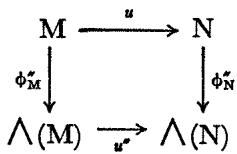
\includegraphics[keepaspectratio]{images/part003_b216bf24.jpg}}

is commutative. Moreover, \(u''\) is a graded algebra homomorphism.

The existence and uniqueness of \(u''\) follow from no. 1, Proposition 1 applied to the algebra \(\bigwedge(\mathbf{N})\) and \(f = \phi_{\mathbf{N}}'' \circ u: \mathbf{M} \to \bigwedge(\mathbf{N})\) ; for \(f(\mathbf{M}) \subset \mathbf{N}\) and hence \(f\) satisfies condition (1) by definition of \(\mathfrak{J}_{\mathbf{N}}''\) : as \(f(\mathbf{M}) \subset \bigwedge^{1}(\mathbf{N}) = \mathbf{N}\) , the fact that \(u''\) is a graded algebra homomorphism follows from Remark 1 of no. 1.

The homomorphism \(u''\) of Proposition 2 will henceforth be denoted by \(\bigwedge(u)\) . If P is an A-module and \(v: \mathbf{N} \to \mathbf{P}\) is an A-linear mapping, then

\[
\bigwedge (v \circ u) = \bigwedge (v) \circ \bigwedge (u)\tag{3}
\]

for \(\bigwedge(v) \circ \bigwedge(u)\) is an algebra homomorphism which renders commutative the diagram

\pandocbounded{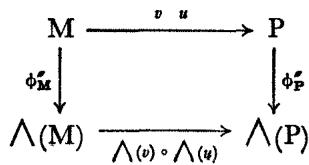
\includegraphics[keepaspectratio]{images/part003_3a522f8d.jpg}}

Since \(\bigwedge (\mathbf{M})\) contains \(\mathbf{M} = \bigwedge^{1}(\mathbf{M}),\bigwedge (u)\) is sometimes called the canonical extension of \(u\) to \(\bigwedge (\mathbf{M})\) . The restriction \(\bigwedge^n (u):\bigwedge^n (\mathbf{M})\to \bigwedge^n (\mathbf{N})\) is such that

\[
\bigwedge^ {n} (u) (x _ {1} \land x _ {2} \land \dots \land x _ {n}) = u (x _ {1}) \land u (x _ {2}) \land \dots \land u (x _ {n})\tag{4}
\]

with the \(x_{i}\in\mathbf{M}\) , since \(\bigwedge(u)\) is an algebra homomorphism and \(\bigwedge^{1}(u)=u\) ; the restriction \(\bigwedge^{0}(u)\) to A is the identity mapping. Note that \(\bigwedge^{n}(u)\) is obtained from \(\mathsf{T}^{n}(u):\mathsf{T}^{n}(\mathbf{M})\to\mathsf{T}^{n}(\mathbf{N})\) by passing to the quotients.

PROPOSITION 3. If \(u: \mathbf{M} \to \mathbf{N}\) is a surjective A-linear mapping, the homomorphism \(\bigwedge(u): \bigwedge(\mathbf{M}) \to \bigwedge(\mathbf{N})\) is surjective and its kernel is the two-sided ideal of \(\bigwedge(\mathbf{M})\) generated by the kernel \(\mathbf{P} \subset \mathbf{M} \subset \bigwedge(\mathbf{M})\) of \(u\) .

The proof is derived from that of §6, no. 2, Proposition 4, replacing S by \(\bigwedge\) and \(\mathfrak{J}'\) by \(\mathfrak{J}''\) .

If \(u: \mathbf{M} \to \mathbf{N}\) is an injective linear mapping, it is not always true that \(\bigwedge(\mathbf{u})\) is an injective mapping (§ 6, Exercise 3) (see however below no. 9, Corollary to Proposition 12). However this is so when \(u\) is an injection such that \(u(\mathbf{M})\) is a direct factor of \(\mathbf{N}\) and then the image of \(\bigwedge(u)\) (isomorphic to \(\bigwedge(\mathbf{M})\) ) is a direct factor of \(\bigwedge(\mathbf{N})\) ; the proof is the same as that for the analogous assertions for \(\mathbf{T}(u)\) (§ 5, no. 2) replacing \(\mathbf{T}\) by \(\bigwedge\) .

PROPOSITION 4. Let N and P be two submodules of an A-module M such that their sum N + P is a direct factor in M and their intersection N ∩ P is a direct factor in N and in P. Then the homomorphisms \(\bigwedge(\mathrm{N}) \to \bigwedge(\mathrm{M})\) , \(\bigwedge(\mathrm{P}) \to \bigwedge(\mathrm{M})\) and \(\bigwedge(\mathrm{N} \cap \mathrm{P}) \to \bigwedge(\mathrm{M})\) , canonical extensions of the canonical injections, are injective; if \(\bigwedge(\mathrm{N})\) , \(\bigwedge(\mathrm{P})\) and \(\bigwedge(\mathrm{N} \cap \mathrm{P})\) are identified with subalgebras of \(\bigwedge(\mathrm{M})\) by means of these homomorphisms, then

\[
\bigwedge (\mathbf {N} \cap \mathbf {P}) = \bigwedge (\mathbf {N}) \cap \bigwedge (\mathbf {P}).\tag{5}
\]

The proof is derived from that of § 5, no. 2, Proposition 4 replacing T by \(\bigwedge\) throughout. The hypotheses of Proposition 4 are always satisfied by arbitrary submodules N, P of M when A is a field.

COROLLARY. Let K be a commutative field and M a vector space over K. For every element \(z \in \bigwedge(\mathbf{M})\) , there exists a smallest vector subspace N of M such that \(z \in \bigwedge(\mathbf{N})\) and N is finite-dimensional.

The proof is deduced from that of § 5, no. 2, Corollary to Proposition 4 replacing T by \(\bigwedge\) throughout.

N is called the vector subspace of M associated with the element z of \(\bigwedge(\mathbf{M})\) .

\subsection{ANTICOMMUTATIVITY OF THE EXTERIOR ALGEBRA}

PROPOSITION 5. (i) Let \((x_{i})_{1\leqslant i\leqslant n}\) be a finite sequence of elements of the module \(\mathbf{M}\) ; for every permutation \(\sigma\) in the symmetric group \(\mathfrak{S}_n\) ,

\[
x _ {\sigma (1)} \wedge x _ {\sigma (2)} \wedge \dots \wedge x _ {\sigma (n)} = \varepsilon_ {\sigma}. x _ {1} \wedge x _ {2} \wedge \dots \wedge x _ {n}\tag{6}
\]

where \(\varepsilon_{\sigma}\) denotes the signature of the permutation \(\sigma\) .

\begin{enumerate}
\def\labelenumi{(\roman{enumi})}
\setcounter{enumi}{1}
\tightlist
\item
  If there exist two distinct indices \(i, j\) such that \(x_{i} = x_{j}\) , the product
\end{enumerate}

\[
x _ {1} \wedge x _ {2} \wedge \dots \wedge x _ {n}
\]

is zero.

\begin{enumerate}
\def\labelenumi{(\roman{enumi})}
\tightlist
\item
  First of all, since \(x \wedge x = 0\) for all \(x \in \mathbf{M}\) by definition of the ideal \(\mathfrak{J}''\) , also, for \(x, y\) in \(\mathbf{M}\) ,
\end{enumerate}

\[
x \wedge y + y \wedge x = (x + y) \wedge (x + y) - x \wedge x - y \wedge y = 0.
\]

This establishes (6) in the case \(n = 2\) . The general case then follows from § 4, no. 6, Lemma 3.

\begin{enumerate}
\def\labelenumi{(\roman{enumi})}
\setcounter{enumi}{1}
\tightlist
\item
  Under the hypothesis of (ii), there exists a permutation \(\sigma \in \mathfrak{S}_n\) such that \(\sigma(1) = i\) and \(\sigma(2) = j\) ; then the left hand side of (6) is zero for this permutation and hence so is the right hand side.
\end{enumerate}

COROLLARY 1. Let H, K be two complementary subsets of the interval \([1, n]\) of N and let \((i_{h})_{1 \leqslant h \leqslant p}, (j_{k})_{1 \leqslant k \leqslant n - p}\) be the sequences of elements of H and K respectively, arranged in increasing order; we write

\[
x _ {H} = x _ {i _ {1}} \wedge x _ {i _ {2}} \wedge \dots \wedge x _ {i _ {p}}, \quad x _ {K} = x _ {j _ {1}} \wedge x _ {j _ {2}} \wedge \dots \wedge x _ {j _ {n - p}};
\]

then

\[
x _ {\mathrm{H}} \wedge x _ {\mathrm{K}} = (- 1) ^ {\nu} x _ {1} \wedge x _ {2} \wedge \dots \wedge x _ {n}\tag{7}
\]

where \(\nu\) is the number of ordered pairs \((i,j)\in \mathbf{H}\times \mathbf{K}\) such that \(i > j\)

By Proposition 5 this reduces to proving

Lemma 1. If \(\sigma \in \mathfrak{S}_n\) is the permutation such that \(\sigma(h) = i_h\) for \(1 \leqslant h \leqslant p\) , \(\sigma(h) = j_{h-p}\) for \(p + 1 \leqslant h \leqslant n\) , then \(\varepsilon_\sigma = (-1)^{\nu}\) .

For \(1 \leqslant h < h' \leqslant p\) or \(p + 1 \leqslant h < h' \leqslant n\) , \(\sigma(h') > \sigma(h)\) and the number of ordered pairs \((h, h')\) such that \(1 \leqslant h \leqslant p < h' \leqslant n\) and \(\sigma(h) > \sigma(h')\) is equal to \(\nu\) .

COROLLARY 2. The graded algebra \(\bigwedge (\mathbf{M})\) is alternating (§ 4, no. 9).

It suffices to apply Proposition 13 of §4, no. 9 to \(\bigwedge (\mathbf{M})\) , taking as generating system the set \(\mathbf{M}\) and using Proposition 5.

PROPOSITION 6. If M is a finitely generated A-module, \(\bigwedge (\mathbf{M})\) is a finitely generated A-module; also, if M admits a generating system with \(n\) elements, then \(\bigwedge^{p}(\mathbf{M}) = \{0\}\) for \(p > n\) .

Let \((x_{i})_{1\leqslant i\leqslant n}\) be a generating system of M. Every element of \(\bigwedge^{p}(\mathbf{M})\) is a linear combination of elements of the form

\[
x _ {i _ {1}} \wedge x _ {i _ {2}} \wedge \dots \wedge x _ {i _ {p}}
\]

where the indices \(i_k\) belong to \([1, n]\) ; by Proposition 5, these indices can be assumed to be distinct (otherwise the corresponding element is zero). If \(p > n\) , there is no such sequence of indices and hence \(\bigwedge^p(\mathbf{M}) = \{0\}\) . If \(p \leqslant n\) , these sequences are finite in number, which completes the proof.

\subsection{n-th EXTERIOR POWER OF A MODULE AND ALTERNATING MULTI-LINEAR MAPPINGS}

Given two modules M, N over a commutative ring A, an alternating n-linear mapping of \(M^{n}\) into N is any n-linear mapping \(f: M^{n} \to N\) such that, for all \(p \leqslant n - 2\) ,

\[
f (u _ {1}, \dots , u _ {p}, x, x, v _ {1}, \dots , v _ {n - p - 2}) = 0\tag{8}
\]

for all \(x\) , the \(u_{i}\) ( \(1 \leqslant i \leqslant p\) ) and the \(v_{j}\) ( \(1 \leqslant j \leqslant n - p - 2\) ) in \(\mathbf{M}\) .

PROPOSITION 7. Let A be a commutative ring and M and N two A-modules. If with every A-linear mapping \(g: \bigwedge^n (\mathbf{M}) \to \mathbf{N} (n \geqslant 2)\) is associated the n-linear mapping

\[
\left(x _ {1}, x _ {2}, \dots , x _ {n}\right) \mapsto g \left(x _ {1} \wedge x _ {2} \wedge \dots \wedge x _ {n}\right)\tag{9}
\]

a bijective A-linear mapping is obtained of the A-module \(\operatorname{Hom}_{\mathbf{A}}(\bigwedge^{n}(\mathbf{M}), \mathbf{N})\) onto the A-module of alternating \(n\) -linear mappings of \(\mathbf{M}^n\) into \(\mathbf{N}\) .

We consider the canonical bijection of the A-module \(\operatorname{Hom}_{\mathbf{A}}(\mathsf{T}^{n}(\mathbf{M}),\mathbf{N})\) onto the A-module \(\mathcal{L}_{n}(\mathbf{M},\ldots,\mathbf{M};\mathbf{N})\) of all n-linear mappings of \(M^{n}\) into N, obtained by associating with every A-linear mapping \(f: T^{n}(\mathbf{M}) \to \mathbf{N}\) the n-linear mapping

\[
\bar {f} \colon (x _ {1}, \dots , x _ {n}) \mapsto f (x _ {1} \otimes x _ {2} \otimes \dots \otimes x _ {n})
\]

(II, § 3, no. 9). On the other hand, the A-linear mappings \(g \colon \bigwedge^{n}(\mathbf{M}) \to \mathbf{N}\) are in one-to-one correspondence with the A-linear mappings \(f \colon \mathsf{T}^n (\mathbf{M}) \to \mathbf{N}\) such that \(f\) is zero on \(\mathfrak{J}_n''\) , by associating with \(g\) the mapping \(f = g \circ p_n\) , where

\[
p _ {n} \colon \mathsf {T} ^ {n} (\mathbf {M}) \rightarrow \bigwedge^ {n} (\mathbf {M}) = \mathsf {T} ^ {n} (\mathbf {M}) / \mathfrak {J} _ {n} ^ {\prime \prime}
\]

is the canonical homomorphism (II, §2, no. 1, Theorem 1). But as \(\mathfrak{J}_n''\) is a linear combination of elements of the form

\[
\left(u _ {1} \otimes u _ {2} \otimes \dots \otimes u _ {p}\right) \otimes (x \otimes x) \otimes \left(v _ {1} \otimes \dots \otimes v _ {n - p - 2}\right)
\]

\((x, u_{i}, v_{j} \text{ in M}), \text{ to say that } f \text{ is of the form } g \circ p_{n} \text{ means that the corresponding } n\text{-linear function } \bar{f} \text{ satisfies (8), in other words it is alternating.}\)

The A-module \(\bigwedge^{n}(\mathbf{M})\) is called the \(n\) -th exterior power of \(\mathbf{M}\) . For every A-module homomorphism \(u: \mathbf{M} \to \mathbf{N}\) , the mapping

\[
\bigwedge^ {n} (u): \bigwedge^ {n} (\mathbf {M}) \rightarrow \bigwedge^ {n} (\mathbf {N})
\]

which coincides with \(\bigwedge(u)\) on \(\bigwedge^{n}(\mathbf{M})\) is called the \(n\) -th exterior power of \(u\) .

COROLLARY 1. For every alternating \(n\) -linear mapping \(g: \mathbf{M}^n \to \mathbf{N}\) , for every permutation \(\sigma \in \mathfrak{S}_n\) ,

\[
g \left(x _ {\sigma (1)}, x _ {\sigma (2)}, \dots , x _ {\sigma (n)}\right) = \varepsilon_ {\sigma}. g \left(x _ {1}, x _ {2}, \dots , x _ {n}\right)\tag{10}
\]

for all \(x_{i} \in \mathbf{M}\) ; moreover if \(x_{i} = x_{j}\) for two distinct indices \(i, j\) , then

\[
g (x _ {1}, x _ {2}, \dots , x _ {n}) = 0.
\]

This is an obvious consequence of Proposition 7 and no. 3, Proposition 5.

COROLLARY 2. Let \((x_{i})_{1\leqslant i\leqslant n}\) be a sequence of \(n\) elements of \(\mathbf{M}\) such that

\[
x _ {1} \wedge x _ {2} \wedge \dots \wedge x _ {n} = 0;
\]

then, for every alternating \(n\) -linear mapping \(g: \mathbf{M}^n \to \mathbf{N}\) , \(g(x_1, \ldots, x_n) = 0\) .

COROLLARY 3. Let \(f: \mathbf{M}^{n-1} \to \mathbf{A}\) be an alternating \((n-1)\) -linear form. If \((x_i)_{1 \leq i \leq n}\) is a sequence of \(n\) elements of \(\mathbf{M}\) such that \(x_1 \wedge x_2 \wedge \cdots \wedge x_n = 0\) , then

\[
\sum_ {i = 1} ^ {n} (- 1) ^ {i} f (x _ {1}, \dots , \hat {x _ {i}}, \dots , x _ {n}). x _ {i} = 0\tag{11}
\]

(where we write \(f(x_{1},\ldots ,\hat{x}_{i},\ldots ,x_{n}) = f(x_{1},\ldots ,x_{i - 1},x_{i + 1},\ldots ,x_{n})\) for \(1\leqslant i\leqslant n\) .

It suffices to prove that the n-linear mapping

\[
(x _ {1}, \dots , x _ {n}) \mapsto \sum_ {i = 1} ^ {n} (- 1) ^ {i} f (x _ {1}, \dots , \hat {x} _ {i}, \dots , x _ {n}). x _ {i}
\]

of \(M^{n}\) to M is alternating. Now, if \(x_{i} = x_{i+1}\) , all the terms in the sum on the right hand side have zero coefficients except \(x_{i}\) and \(x_{i+1}\) , since f is alternating; on the other hand, the coefficient of \(x_{i}\) is

\[
(- 1) ^ {i} f (x _ {1}, \dots , x _ {i - 1}, x _ {i + 1}, x _ {i + 2}, \dots , x _ {n})
\]

and that of \(x_{i+1}\) is \((-1)^{i+1}f(x_1, \ldots, x_i, x_{i+2}, \ldots, x_n)\) and they are inverses by hypothesis.

Remark. An element \(z\) of \(\mathsf{T}^n (\mathbf{M})\) is called a (contravariant) skew-symmetric tensor of order \(n\) if \(\sigma .z = \varepsilon_{\sigma}z\) for every permutation \(\sigma \in \mathfrak{S}_n\) (cf.~§6, no. 3, Remark); these elements form a sub-A-module \(\mathsf{A}_n^\prime (\mathbf{M})\) of \(\mathsf{T}^n (\mathbf{M})\) . For all \(z\in \mathsf{T}^n (\mathbf{M})\) , we write \(\pmb {a}.z = \sum_{\sigma \in \mathfrak{S}_n}\varepsilon_\sigma (\sigma .z)\) and call \(\pmb {a}.z\) the skew-symmetrization of \(z\) ; as \(\varepsilon_{\sigma \tau} = \varepsilon_{\sigma}\varepsilon_{\tau}\) , it is immediately seen that \(\pmb {a}.z\) is a skew-symmetric tensor and therefore \(z\mapsto \pmb {a}.z\) is an endomorphism of \(\mathsf{T}^n (\mathbf{M})\) whose image \(\mathsf{A}_n''(\mathbf{M})\) is contained in \(\mathsf{A}_n^\prime (\mathbf{M})\) ; in general \(\mathsf{A}_n''(\mathbf{M})\neq \mathsf{A}_n^\prime (\mathbf{M})\) (Exercise 8). If \(z\) is a skew-symmetric tensor, then \(\pmb {a}.z = n!z\) ; hence, when \(n!\) is invertible in A, the endomorphism \(z\mapsto (n!)^{-1}\pmb {a}.z\) is a projector of \(\mathsf{T}^n (\mathbf{M})\) whose image is

\[
\mathbf {A} _ {n} ^ {\prime} (\mathbf {M}) = \mathbf {A} _ {n} ^ {\prime \prime} (\mathbf {M}).
\]

Moreover the kernel of this projector is just \(\mathfrak{J}_n''\) ; for attention may obviously be confined to the case where \(n \geqslant 2\) , hence 2 (a divisor of \(n!\) ) is invertible in A and \(x \otimes x = 2^{-1}(x \otimes x + x \otimes x)\) ; therefore \(\mathfrak{J}_n''\) is generated by the elements \(z + \rho . z\) , where \(\rho\) is a transposition exchanging two consecutive numbers in \([1, n]\) ; moreover, for two permutations \(\sigma, \tau\) in \(\mathfrak{S}_n\) , we can write

\[
z - \varepsilon_ {\sigma \tau} ((\sigma \tau). z) = z - \varepsilon_ {\tau} (\tau . z) + \varepsilon_ {\tau} (\tau . z - \varepsilon_ {\sigma} \sigma . (\tau . z))
\]

whence it follows that \(z - \varepsilon_{\sigma}(\sigma . z) \in \mathfrak{J}_{n}^{\prime \prime}\) for all \(z \in \mathbf{T}^{n}(\mathbf{M})\) and \(\sigma \in \mathfrak{S}_{n}\) . Therefore (always assuming \(n!\) is invertible in A), it is seen that

\[
z - (n!) ^ {- 1} \boldsymbol {a}. z = \sum_ {\sigma \in \mathfrak {S} _ {n}} (n!) ^ {- 1} (z - \varepsilon_ {\sigma} (\sigma . z)) \in \mathfrak {J} _ {n} ^ {\prime \prime}
\]

for all \(z \in \mathbf{T}^n(\mathbf{M})\) , which establishes our assertion.

When \(n!\) is invertible in A, the submodules \(\mathsf{A}_n'(M)\) and \(\mathfrak{J}_n''\) of \(T^n(M)\) are therefore supplementary and the restriction to \(\mathsf{A}_n'(M)\) of the canonical homomorphism \(T^n(M) \to \bigwedge^n(M) = T^n(M)/\mathfrak{J}_n''\) is an A-module isomorphism, which allows us in the case in question to identify skew-symmetric tensors of order \(n\) with the elements of the \(n\) -th exterior power of M. Note here also that this identification is not compatible with multiplication, the product in \(T(M)\) of two skew-symmetric tensors not being skew-symmetric in general.

\subsection{EXTENSION OF THE RING OF SCALARS}

Let A, A' be two commutative rings, \(\rho:A\to A'\) a ring homomorphism, M an A-module, M' an A'-module and \(f:M\to M'\) an A-homomorphism (relative to \(\rho\) ) of M into M'. The composite mapping \(M\xrightarrow{f}M'\xrightarrow{\phi_{M'}^{\prime\prime}}\bigwedge_{A'(M')}\) is an A-linear mapping of M into the A-algebra \(\bigwedge_{A'(M')}\) and, as the elements of \(f(\mathbf{M}) \subset \mathbf{M}'\) are of zero square in \(\bigwedge_{\mathbf{A}'}(\mathbf{M}')\) , there exists (no. 1, Proposition 1) one and only one A-homomorphism of algebras \(f'': \bigwedge_{\mathbf{A}}(\mathbf{M}) \to \bigwedge_{\mathbf{A}'}(\mathbf{M}')\) rendering commutative the diagram

\begin{enumerate}
\def\labelenumi{(\arabic{enumi})}
\setcounter{enumi}{11}
\tightlist
\item
\end{enumerate}

\pandocbounded{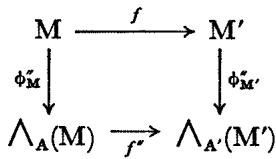
\includegraphics[keepaspectratio]{images/part003_899f4c21.jpg}}

and \(f''\) is a graded algebra homomorphism. It is immediately deduced that if \(\sigma: A' \to A''\) is another ring homomorphism, \(M''\) an \(A''\) -module, \(g: M' \to M''\) an \(A'\) -homomorphism (relative to \(\sigma\) ) and \(g'': \bigwedge_{A'}(M') \to \bigwedge_{A''}(M'')\) the corresponding \(A''\) -homomorphism of algebras, then the composite A-homomorphism of algebras

\[
\bigwedge_ {\mathbf {A}} (\mathbf {M}) \xrightarrow {f ^ {\prime \prime}} \bigwedge_ {\mathbf {A} ^ {\prime}} (\mathbf {M} ^ {\prime}) \xrightarrow {g ^ {\prime \prime}} \bigwedge_ {\mathbf {A} ^ {\prime \prime}} (\mathbf {M} ^ {\prime \prime})\tag{13}
\]

corresponds to the composite A-homomorphism \(g \circ f: \mathbf{M} \to \mathbf{M}''\) (relative to \(\sigma \circ \rho\) ).

PROPOSITION 8. Let A, B be two commutative rings, \(\rho: A \to B\) a ring homomorphism and M an A-module. The canonical extension

\[
\psi : \bigwedge_ {\mathbf {B}} (\mathbf {B} \otimes_ {\mathbf {A}} \mathbf {M}) \rightarrow \mathbf {B} \otimes_ {\mathbf {A}} \bigwedge_ {\mathbf {A}} (\mathbf {M})
\]

of the B-linear mapping \(l_{B} \otimes \phi_{M}^{\prime\prime}: B \otimes_{A} M \to B \otimes_{A} \bigwedge_{A}(M)\) is a graded B-algebra isomorphism.

The proof is derived from that of § 5, no. 4, Proposition 5 replacing T by \(\bigwedge\) and \(\phi_{\mathbf{M}}\) by \(\phi_{\mathbf{M}}^{\prime \prime}\) .

\subsection{DIRECT LIMITS OF EXTERIOR ALGEBRAS}

Let \((\mathbf{A}_{\alpha},\phi_{\beta \alpha})\) be a directed direct system of commutative rings, \((\mathbf{M}_{\alpha},f_{\beta \alpha})\) a direct system of \(\mathbf{A}_{\alpha}\) -modules, \(\mathbf{A} = \varinjlim \mathbf{A}_{\alpha}\) and \(\mathbf{M} = \varinjlim \mathbf{M}_{\alpha}\) . For \(\alpha \leqslant \beta\) , we derive canonically from the \(\mathbf{A}_{\alpha}\) -homomorphism \(f_{\beta \alpha}: \overrightarrow{\mathbf{M}_{\alpha}} \to \mathbf{M}_{\beta}\) an \(\mathbf{A}_{\alpha}\) -algebra homomorphism (no. 5, formula (12)) \(f_{\beta \alpha}^{\prime \prime}: \bigwedge_{\mathbf{A}_{\alpha}} (\mathbf{M}_{\alpha}) \to \bigwedge_{\mathbf{A}_{\beta}} (\mathbf{M}_{\beta})\) and it follows from (13) that \((\bigwedge_{\mathbf{A}_{\alpha}} (\mathbf{M}_{\alpha}), f_{\beta \alpha}^{\prime \prime})\) is a direct system of graded \(\mathbf{A}_{\alpha}\) -modules. On the other hand let \(f_{\alpha}: \mathbf{M}_{\alpha} \to \mathbf{M}\) be the canonical \(\mathbf{A}_{\alpha}\) -homomorphism; we derive (no. 5, formula (12)) a graded \(\mathbf{A}_{\alpha}\) -algebra homomorphism \(f_{\alpha}^{\prime \prime}: \bigwedge_{\mathbf{A}_{\alpha}} (\mathbf{M}_{\alpha}) \to \bigwedge_{\mathbf{A}} (\mathbf{M})\) and it also follows from (13) that the \(f_{\alpha}^{\prime \prime}\) constitute a direct system of \(\mathbf{A}_{\alpha}\) -homomorphisms.

PROPOSITION 9. The A-homomorphism \(f'' = \varinjlim f_{\alpha}' : \varinjlim \bigwedge_{A_{\alpha}}(M_{\alpha}) \to \bigwedge_{A}(M)\) is a graded algebra isomorphism.

The proof is the same as that of § 5, no. 4, Proposition 6 replacing throughout T by \(\bigwedge\) and \(\phi\) by \(\phi''\) and taking account of the fact that a direct limit of alternating algebras is alternating.

\subsection{EXTERIOR ALGEBRA OF A DIRECT SUM. EXTERIOR ALGEBRA OF A GRADED MODULE}

Let A be a commutative ring, \(M = \bigoplus_{\lambda \in L} M_{\lambda}\) the direct sum of a family of a family of A-modules and \(j_{\lambda}: M_{\lambda} \to M\) the canonical injection; an A-homomorphism of graded algebras \(\bigwedge(j_{\lambda}): \bigwedge(M_{\lambda}) \to \bigwedge(M)\) is derived. Since \(\bigwedge(M)\) is anticommutative, Proposition 10 of §4, no. 7 (or if need be generalized to the case where L is infinite, cf.~§4, no. 8, Remark 1) can be applied to the homomorphisms \(\bigwedge(j_{\lambda})\) ; then there exists a unique algebra homomorphism

\[
g \colon \bigotimes_ {\lambda \in L} ^ {g} \Lambda (M _ {\lambda}) \to \Lambda (M)\tag{14}
\]

(also denoted by \(g_{\mathbf{M}}\) ) such that \(\bigwedge (j_{\lambda}) = g \circ f_{\lambda}\) , where

\[
f _ {\lambda}: \bigwedge (\mathrm{M} _ {\lambda}) \rightarrow \bigotimes_ {\lambda \in L} ^ {g} \bigwedge (\mathrm{M} _ {\lambda})
\]

denotes the canonical homomorphism.

PROPOSITION 10. The canonical homomorphism \(g\) (formula (14)) is a graded algebra isomorphism.

To prove that \(g\) is bijective, we define a graded algebra homomorphism

\[
h: \bigwedge (\mathbf {M}) \rightarrow \bigotimes_ {\lambda \in L} ^ {\mathfrak {g}} \bigwedge (\mathbf {M} _ {\lambda})\tag{15}
\]

such that \(g \circ h\) and \(h \circ g\) are respectively the identity mappings on \(\bigwedge(\mathbf{M})\) and \(\bigotimes_{\lambda \in L} \bigwedge(\mathbf{M}_{\lambda})\) . For each \(\lambda \in L\) , consider the composite linear mapping

\[
u _ {\lambda}: \mathrm{M} _ {\lambda} \xrightarrow {\phi_ {\mathrm{M} _ {\lambda}} ^ {n}} \bigwedge (\mathrm{M} _ {\lambda}) \xrightarrow {f _ {\lambda}} \mathbf {g} _ {\lambda \in L} \bigotimes \bigwedge (\mathrm{M} _ {\lambda}).
\]

There exists one and only one A-linear mapping \(u: \mathbf{M} \to {}^{\mathfrak{g}} \bigotimes_{\lambda \in L} \bigwedge (\mathbf{M}_{\lambda})\) such that \(u \circ j_{\lambda} = u_{\lambda}\) for all \(\lambda \in L\) . The skew tensor product \({}^{\mathfrak{g}} \bigotimes_{\lambda \in L} \bigwedge (\mathbf{M}_{\lambda})\) is an alternating algebra: for, for L finite, this follows from § 4, no. 9, Proposition 14 and, for L arbitrary, this follows from the definition of this product given in § 4, no. 8, Remark 1 and the fact that a direct limit of alternating graded algebras is alternating. As also \(u(\mathbf{M})\) is contained in the submodule of elements of degree 1 in the graded algebra \(\bigotimes_{\lambda \in L} \bigwedge (\mathbf{M}_{\lambda})\) , it follows from no. 1, Proposition 1 and Remark 1 that there exists a unique graded algebra homomorphism.

\[
h: \bigwedge (\mathbf {M}) \rightarrow \bigotimes_ {\lambda \in L} ^ {\mathfrak {g}} \bigwedge (\mathbf {M} _ {\lambda})
\]

such that \(h \circ \phi_{\mathbf{M}}'' = u\) . The verification of the fact that \(g \circ h\) and \(h \circ g\) are the identity mappings is then performed as in §6, no. 6, Proposition 9 replacing \(\mathbf{S}\) by \(\bigwedge\) and \(\phi'\) by \(\phi''\) .

Remark. Let \(N = \bigoplus_{\lambda \in L} N_{\lambda}\) be the direct sum of another family of A-modules with L as indexing set and, for all \(\lambda \in L\) , let \(v_{\lambda}: M_{\lambda} \to N_{\lambda}\) be an A-linear mapping, whence there is an A-linear mapping \(v = \bigoplus_{\lambda} v_{\lambda}: M \to N\) (II, §1, no. 6, Proposition 7). Then the diagram

\[
\begin{array}{c c c} \mathbf {g} _ {\lambda \in L} ^ {\otimes} \wedge (\mathrm{M} _ {\lambda}) & \xrightarrow {g _ {\mathrm{M}}} & \wedge (\mathrm{M}) \\ \bigotimes_ {\lambda \in L} \wedge (v _ {\lambda}) \Big \downarrow & & \Big \downarrow \wedge (v) \\ \mathbf {g} _ {\lambda \in L} ^ {\otimes} \wedge (\mathrm{N} _ {\lambda}) & \xrightarrow {g _ {\mathrm{N}}} & \wedge (\mathrm{N}) \end{array}
\]

is commutative (cf.~§ 4, no. 5, Corollary to Proposition 8).

The sub-A-module of \(\mathbf{g}_{\lambda \in L}^{\otimes} \bigwedge (\mathbf{M}_{\lambda})\) with which \(\bigwedge^{n}(\mathbf{M})\) is identified by means of the isomorphism \(g\) can be described more precisely. For every finite subset \(J\) of \(L\) , we write \(\mathrm{E}_{J} = \mathbf{g}_{\lambda \in J}^{\otimes} \bigwedge (\mathbf{M}_{\lambda})\) , so that \(\mathbf{g}_{\lambda \in L}^{\otimes} \bigwedge (\mathbf{M}_{\lambda}) = \lim_{\lambda \to 0} \mathrm{E}_{J}\) relative to the directed set \(\mathfrak{F}(L)\) of finite subsets of \(L\) , by definition (§ 4, no. 8, Remark 1). For every family \(\nu = (n_{\lambda}) \in \mathbf{N}^{(L)}\) (therefore with finite support) such that \(\sum_{\lambda \in L} n_{\lambda} = n\) and every finite subset \(J\) of \(L\) containing the support of the family \(\nu\) , we write

\[
\bigwedge^ {J, v} (\mathbf {M}) = \bigotimes_ {\lambda \in J} \bigwedge^ {n _ {\lambda}} (\mathbf {M} _ {\lambda})\tag{16}
\]

so that the submodule \(\mathbf{E}_{\mathbf{J},n}\) of elements of degree \(n\) in \(\mathbf{E}_{\mathbf{J}}\) is the direct sum of the \(\bigwedge^{\mathbf{J},\nu}(\mathbf{M})\) for all families \(\nu\) of support contained in \(\mathbf{J}\) and such that

\[
\sum_ {\lambda \in L} n _ {\lambda} = n
\]

(§ 4, no. 7, Proposition 10 and no. 8). By way of convention we write \(\bigwedge^{J,\nu}(\mathbf{M}) = \{0\}\) for the families \(\nu\) whose support is not contained in \(J\) ; then

\(E_{J,n}\) can also be called the direct sum of all the \(\bigwedge^{J,\nu}(M)\) , where \(\nu\) runs through the set \(H_n\) of all families \(\nu = (n_\lambda)_{\lambda \in L}\) such that \(\sum_{\lambda \in L} n_\lambda = n\) . Since \(\bigwedge^0(M_\lambda)\) is identified with A, clearly also for two finite subsets \(J \subset J'\) of L and a family \(\nu\) of support contained in J, the canonical mapping \(\bigwedge^{J,\nu}(M) \to \bigwedge^{J',\nu}(M)\) (restriction of the canonical mapping \(E_J \to E_{J'}\) to \(\bigwedge^{J,\nu}(M)\) ) is bijective. If we write, for all \(\nu \in H_n\) ,

\[
\bigwedge^ {\nu} (\mathbf {M}) = \varinjlim \bigwedge^ {J, \nu} (\mathbf {M})\tag{17}
\]

it is then seen that, taking account of II, § 6, no. 2, Proposition 5, we have:

COROLLARY. The A-module \(\bigwedge^{n}(\mathbf{M})\) is the image under isomorphism (14) of the submodule of \(\bigotimes_{\lambda \in L} \bigwedge (\mathbf{M}_{\lambda})\) the direct sum of the submodules \(\bigwedge^{\nu}(\mathbf{M})\) for all families \(\nu = (n_{\lambda}) \in \mathbf{N}^{(L)}\) such that \(\sum_{\lambda \in L} n_{\lambda} = n\) ; if \(J\) is the support of \(\nu, \bigwedge^{\nu}(\mathbf{M})\) is canonically isomorphic to \(\bigotimes_{\lambda \in J} \bigwedge^{n_{\lambda}}(\mathbf{M}_{\lambda})\) .

In general \(\bigwedge^{\nu}(\mathbf{M}),\bigotimes_{\lambda \in J}\bigwedge^{n_{\lambda}}(\mathbf{M}_{\lambda})\) and their image in \(\bigwedge^n (\mathbf{M})\) are identified. With this convention:

PROPOSITION 11. Let \(\Delta\) be a commutative monoid, \(\mathbf{M}\) a graded A-module of type \(\Delta\) and \((\mathbf{M}_{\alpha})_{\alpha \in \Delta}\) its graduation. For every ordered pair \((\alpha, n) \in \Delta \times \mathbf{N}\) , let \(\bigwedge^{\alpha, n}(\mathbf{M})\) be the submodule of \(\bigwedge^n (\mathbf{M})\) the direct sum of the submodules \(\bigotimes_{\lambda \in J} \bigwedge^{n_{\lambda}}(\mathbf{M}_{\alpha_{\lambda}})\) , where \((n_{\lambda})_{\lambda \in L}\) runs through the set of families of integers \(\geqslant 0\) such that \(\sum_{\lambda \in L} n_{\lambda} = n\) , \(J\) is its support and, for each \((n_{\lambda})\) , \((\alpha_{\lambda})_{\lambda \in J}\) runs through the set of families of \(\Delta^J\) such that \(\sum_{\lambda \in J} \alpha_{\lambda} = \alpha\) . Then \((\bigwedge^{\alpha, n}(\mathbf{M}))_{(\alpha, n) \in \Delta \times N}\) is the only graduation of type \(\Delta \times N\) compatible with the algebra structure on \(\bigwedge(\mathbf{M})\) and which induces on \(\mathbf{M} = \bigwedge^1 (\mathbf{M})\) the given graduation.

The fact that \(\bigwedge (\mathbf{M})\) is the direct sum of the \(\bigwedge^{\alpha ,n}(\mathbf{M})\) follows from the Corollary to Proposition 10; the rest of the proof is identical with the end of the proof of §5, no. 5, Proposition 7.

\subsection{EXTERIOR ALGEBRA OF A FREE MODULE}

THEOREM 1. Let M be an A-module with a basis \((e_{\lambda})_{\lambda \in L}\) . Let L be given the structure of a totally ordered set (Set Theory, III, §2, no. 3, Theorem 1) and for every finite subset J of L we write

\[
e _ {J} = e _ {\lambda_ {1}} \wedge e _ {\lambda_ {2}} \wedge \dots \wedge e _ {\lambda_ {n}}\tag{18}
\]

where \((\lambda_k)_{1 \leqslant k \leqslant n}\) is the sequence of elements of \(J\) arranged in increasing order (Set Theory, III, § 5, no. 3, Proposition 6); we write \(e_\varphi = 1\) , the unit element of A. Then the \(e_J\) , where \(J\) runs through the set \(\mathfrak{F}(L)\) of finite subsets of \(L\) , form a basis of the exterior algebra \(\bigwedge(M)\) .

Since the \(e_{\lambda}\) generate the A-module M, every element of \(\bigwedge(\mathbf{M})\) is a linear combination of a finite number of products of the elements \(e_{\lambda}\) and hence (taking account of no. 3, Proposition 5) is a linear combination of a finite number of elements \(e_{J}\) for \(J \in \mathfrak{F}(L)\) . It reduces to proving that the \(e_{J}\) are linearly independent over A. Otherwise, there would exist between these elements a linear relation with coefficients not all zero; the union of the subsets J which correspond to the \(e_{J}\) whose coefficients in this relation are \(\neq 0\) is a finite subset K of L (since there is only a finite number of coefficients \(\neq 0\) ). Let N be the submodule of M generated by the \(e_{\lambda}\) such that \(\lambda \in K\) ; N is a direct factor in M, hence (no. 2) \(\bigwedge(\mathbf{N})\) is identified with a subalgebra of \(\bigwedge(\mathbf{M})\) and, if we show that the \(e_{J}\) with \(J \subset K\) form a basis of \(\bigwedge(\mathbf{N})\) , we shall obtain the desired contradiction.

It therefore reduces to providing Theorem 1 when the basis of M is finite; we may therefore suppose that \(L = [1, m] \subset N\) . For each \(i \in L\) , let \(M_i\) be the free submodule \(Ae_i\) of M; M is the direct sum of the \(M_i\) and \(\bigwedge(M_i)\) is the direct sum of \(\bigwedge^0(M_i) = A\) and \(\bigwedge^1(M_i) = M_i\) (no. 3, Proposition 6). Let \(\bigwedge(M)\) be canonically identified with the A-module the tensor product of the \(\bigwedge(M_i)\) (no. 7, Proposition 10); the latter has as basis the tensor product of the bases \((1, e_i)\) of the \(\bigwedge(M_i)\) (II, § 3, no. 7, Corollary 2 to Proposition 7); thus we obtain all the elements

\[
u _ {1} \otimes u _ {2} \otimes \dots \otimes u _ {m}
\]

where either \(u_{i}=1\) or \(u_{i}=e_{i}\) ; if J is the set of indices i such that \(u_{i}=e_{i}\) , \(u_{1}\otimes u_{2}\otimes\cdots\otimes u_{m}\) is identical with \(e_{J}\) , which completes the proof.

COROLLARY 1. Suppose that \(\mathbf{L} = [1, m]\) ; then the basis \((e_{\mathrm{J}})_{\mathrm{J} \in \mathfrak{P}(\mathrm{L})}\) of \(\bigwedge (\mathbf{M})\) has \(2^{m}\) elements. For \(p > m\) , \(\bigwedge^{p}(\mathbf{M}) = \{0\}\) ; \(\bigwedge^{m}(\mathbf{M})\) has a basis consisting of a single element \(e_{\mathrm{L}}\) ; for \(0 \leqslant p \leqslant m\) the number of elements in the basis \((e_{\mathrm{J}})\) of \(\bigwedge^{p}(\mathbf{M})\) consisting of the \(e_{\mathrm{J}}\) such that \(\operatorname{Card}(\mathbf{J}) = p\) is

\[
\binom {m} {p} = \frac {m !}{p ! (m - p) !}.
\]

This follows from Set Theory, III, § 3, no. 5, Proposition 12 and Set Theory, III, § 5, no. 8, Corollary 1 to Proposition 11.

We return to the case where the set L in Theorem 1 is arbitrary and give explicitly the multiplication table (§ 1, no. 7) of the basis \((e_{J})\) . Given two finite subsets \(J\) , \(K\) of the totally ordered set \(L\) , we write

\[
\left\{ \begin{array}{l l} \rho_ {J, K} = 0 & \text { if } J \cap K \neq \varnothing \\ \rho_ {J, K} = (- 1) ^ {\nu} & \text { if } J \cap K = \varnothing \end{array} \right.\tag{19}
\]

where v denotes the number of ordered pairs \((\lambda, \mu) \in J \times K\) such that \(\lambda > \mu\) . Then Corollary 1 to Proposition 4 of no. 2 immediately implies the relation

\[
e _ {J} \wedge e _ {K} = \rho_ {J, K} e _ {J \cup K}.\tag{20}
\]

Note the formula

\[
\rho_ {J, K} \rho_ {K, J} = (- 1) ^ {j k}\tag{21}
\]

when \(\mathbf{J} \cap \mathbf{K} = \varnothing, j = \operatorname{Card}(\mathbf{J}), k = \operatorname{Card}(\mathbf{K})\) (no. 3, Corollary 2 to Proposition 5.)

COROLLARY 2. If M is a projective A-module, \(\bigwedge (\mathbf{M})\) is a projective A-module.

The proof is the same as that of § 5, no. 5, Corollary to Theorem 1 replacing T by \(\Lambda\) .

COROLLARY 3. Let M be a projective A-module and \((x_{i})_{1\leqslant i\leqslant n}\) a finite sequence of elements of M. For there to exist on M an alternating \(n\) -linear form \(f\) such that

\[
f (x _ {1}, x _ {2}, \dots , x _ {n}) \neq 0,
\]

it is necessary and sufficient that \(x_{1} \wedge x_{2} \wedge \cdots \wedge x_{n} \neq 0\) .

We know already (with no hypothesis on M) that the condition is necessary (no. 4, Proposition 7). Suppose now that M is projective and that

\[
x _ {1} \wedge x _ {2} \wedge \dots \wedge x _ {n} \neq 0.
\]

Then \(\bigwedge^n (\mathbf{M})\) is projective (Corollary 2) and hence the canonical mapping

\[
\bigwedge^ {n} (\mathbf {M}) \rightarrow (\bigwedge^ {n} (\mathbf {M})) ^ {* *}
\]

is injective (II, §2, no. 7, Corollary 4 to Proposition 13); we conclude that there exists a linear form \(g: \bigwedge^{n}(\mathbf{M}) \to \mathbf{A}\) such that \(g(x_{1} \wedge x_{2} \wedge \dots \wedge x_{n}) \neq 0\) . If \(f\) is the alternating \(n\) -linear form corresponding to \(g\) (no. 4, Proposition 7), then \(f(x_{1}, \ldots, x_{n}) \neq 0\) .

\subsection{CRITERIA FOR LINEAR INDEPENDENCE}

PROPOSITION 12. Let M be a projective A-module. For elements \(x_1, x_2, \ldots, x_n\) of M to be linearly dependent, it is necessary and sufficient that there exist \(\lambda \neq 0\) in A such that

\[
\lambda x _ {1} \wedge x _ {2} \wedge \dots \wedge x _ {n} = 0.\tag{22}
\]

The condition is necessary (with no hypothesis on M), for if for example \(\lambda x_{1}\) (with \(\lambda \neq 0\) ) is a linear combination of \(x_{2}, \ldots, x_{n}\) , relation (22) holds (no. 3, Proposition 5). We show that the condition is sufficient by induction on n; for n = 1, it is a trivial consequence of the definition. Suppose therefore that n \textgreater{} 1 and that condition (22) holds for some \(\lambda \neq 0\) . If

\[
\lambda x _ {2} \wedge x _ {3} \wedge \dots \wedge x _ {n} = 0,
\]

then the induction hypothesis implies that \(x_{2},\ldots,x_{n}\) are linearly dependent and hence a fortiori \(x_{1},x_{2},\ldots,x_{n}\) are. If \(\lambda x_{2}\wedge x_{3}\wedge\cdots\wedge x_{n}\neq0\) , it follows from no. 8, Corollary 3 to Theorem 1 that there exists an alternating \((n-1)\) -linear form f such that \(f(\lambda x_{2}\wedge x_{3}\wedge\cdots\wedge x_{n})=\mu\neq0\) . Since

\[
x _ {1} \wedge (\lambda x _ {2}) \wedge \dots \wedge x _ {n} = 0,
\]

it follows from no. 8, Corollary 3 to Theorem 1 that \(\mu x_{1}\) is a linear combination of \(\lambda x_{2}, x_{3}, \ldots, x_{n}\) ; hence \(x_{1}, x_{2}, \ldots, x_{n}\) are linearly dependent.

COROLLARY. Let M and N be two projective A-modules and \(f:M\to N\) an A-linear mapping. If f is injective, then \(\bigwedge(f):\bigwedge(\mathbf{M})\to\bigwedge(\mathbf{N})\) is injective.

We prove this first under the assumption that M is free; let \((e_{\lambda})_{\lambda \in L}\) be a basis of M, so that \((e_{J})_{J \in \mathfrak{F}(L)}\) (formula (18)) is a basis of \(\bigwedge(M)\) . Suppose that the kernel of \(\bigwedge(f)\) contains an element \(u = \sum_{J} \alpha_{J} e_{J} \neq 0\) . Let K be an element minimal among the finite subsets J such that \(\alpha_{J} \neq 0\) and let H be a finite subset of L disjoint from K and such that \(K \cup H\) contains all the J (finite in number) such that \(\alpha_{J} \neq 0\) ; for all \(J \neq K\) such that \(\alpha_{J} \neq 0\) , we have therefore by definition \(J \cap H \neq 0\) and consequently (no. 8, formula (20)).

\[
u \wedge e _ {\mathrm{H}} = + \alpha_ {\mathbf {K}} e _ {\mathbf {K} \cup \mathbf {H}}
\]

belongs to the two-sided ideal of \(\bigwedge (\mathbf{M})\) , the kernel of \(\bigwedge (f)\) . We write \(e_{\mathbf{K} \cup \mathbf{H}} = e_{\lambda_1} \wedge e_{\lambda_2} \wedge \dots \wedge e_{\lambda_n}\) ; then \(\alpha_{\mathbf{K}} f(e_{\lambda_1}) \wedge f(e_{\lambda_2}) \wedge \dots \wedge f(e_{\lambda_n}) = 0\) ; by virtue of Proposition 12, the elements \(f(e_{\lambda_i})\) ( \(1 \leqslant i \leqslant n\) ) of N are linearly dependent. But this contradicts the hypothesis that \(f\) is injective (II, §1, no. 11, Corollary 3 to Proposition 17).

We now consider the general case; let \(\mathbf{M}'\) be an A-module such that \(\mathbf{M} \oplus \mathbf{M}' = \mathbf{P}\) is free (II, § 2, no. 2, Proposition 4). Consider the linear mapping \(g: \mathbf{M} \oplus \mathbf{M}' \to \mathbf{N} \oplus \mathbf{M} \oplus \mathbf{M}'\) such that \(g(x, y) = (f(x), 0, y)\) , so that there is a commutative diagram

\pandocbounded{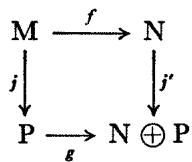
\includegraphics[keepaspectratio]{images/part004_a147f11a.jpg}}

where the vertical arrows are the canonical injections. Since g is injective and P is free, \(\bigwedge(g)\) is an injective homomorphism as has been seen above. Now, \(\bigwedge(j):\bigwedge(\mathbf{M})\to\bigwedge(\mathbf{P})\) is an injective homomorphism since M is a direct factor in P (no. 2). The composite homomorphism

\[
\bigwedge (\mathbf {M}) \xrightarrow {\bigwedge (j)} \bigwedge (\mathbf {P}) \xrightarrow {\bigwedge (g)} \bigwedge (\mathbf {N} \oplus \mathbf {P})
\]

is therefore injective and, as it is also equal to the composite homomorphism

\[
\Lambda (\mathbf {M}) \xrightarrow {\Lambda (f)} \Lambda (\mathbf {N}) \xrightarrow {\Lambda (j ^ {\prime})} \Lambda (\mathbf {N} \oplus \mathbf {P})
\]

we conclude that \(\bigwedge (f)\) is injective.

PROPOSITION 13. Let M be an A-module, N a direct factor submodule of M which is free of dimension p and \(\{u\}\) a basis of \(\bigwedge^{p}(\mathbf{N})\) . For an element \(x \in M\) to belong to N, it is necessary and sufficient that \(u \wedge x = 0\) .

Let P be a submodule of M complementary to N and let \(y \in N\) , \(z \in P\) be such that \(x = y + z\) . Then \(u \wedge x = u \wedge z\) . As \(\bigwedge^{p}(N)\) is free of dimension 1, the mapping \(\phi: P \to P \otimes \bigwedge^{p}(N)\) such that \(\phi(p) = p \otimes u\) is bijective (II, §3, no. 4, Proposition 4). On the other hand (no. 7, Proposition 10), the composition of the canonical homomorphisms

\[
\psi : \mathrm{P} \otimes \bigwedge^ {p} (\mathrm{N}) \rightarrow \bigwedge (\mathrm{P}) \otimes \bigwedge (\mathrm{N}) \rightarrow \bigwedge (\mathrm{M})
\]

is injective. The mapping \(\psi \circ \phi\) is therefore injective, whence the proposition.

THEOREM 2. Let \(\mathbf{M}\) be an A-module with a finite basis \((e_i)_{1\leqslant i\leqslant n}\) . For a sequence \((x_i)_{1\leqslant i\leqslant n}\) of \(n\) elements of \(\mathbf{M}\) to form a basis of \(\mathbf{M}\) , it is necessary and sufficient that the element \(\lambda \in \mathbf{A}\) such that

\[
x _ {1} \wedge x _ {2} \wedge \dots \wedge x _ {n} = \lambda . e _ {1} \wedge e _ {2} \wedge \dots \wedge e _ {n}\tag{23}
\]

be invertible in A.

Recall that \(e_{1} \wedge e_{2} \wedge \cdots \wedge e_{n}\) is the unique element of a basis of \(\bigwedge^{n}(\mathbf{M})\) (no. 8, Corollary 1 to Theorem 1) so that the element \(\lambda \in A\) satisfying (23) is determined uniquely. If \((x_{i})_{1 \leqslant i \leqslant n}\) is a basis of M, \(x_{1} \wedge x_{2} \wedge \cdots \wedge x_{n}\) is the unique element in a basis of \(\bigwedge^{n}(\mathbf{M})\) (no. 8), then \(\lambda\) is invertible. Conversely, suppose \(\lambda\) is invertible; then the alternating n-linear form f corresponding to the linear mapping \(g: \bigwedge^{n}(\mathbf{M}) \to \mathbf{A}\) such that

\[
g (e _ {1} \wedge e _ {2} \wedge \dots \wedge e _ {n}) = \lambda^ {- 1}
\]

is such that \(f(x_{1}, x_{2}, \ldots, x_{n}) = 1\) . For all \(x \in \mathbf{M}\) , obviously

\[
x \wedge x _ {1} \wedge \dots \wedge x _ {n} = 0
\]

(no. 3, Proposition 6); applying no. 8, Corollary 3 to Theorem 1, we obtain

\[
f (x _ {1}, x _ {2}, \dots , x _ {n}). x = \sum_ {i = 1} (- 1) ^ {i - 1} f (x, x _ {1}, \dots , \hat {x} _ {i}, \dots , x _ {n}). x _ {i}.
\]

As \(f(x_{1},\ldots ,x_{n}) = 1\) , this shows that every \(x\in \mathbf{M}\) is a linear combination of \(x_{1},x_{2},\ldots ,x_{n}\) and, as the latter are linearly independent (since

\[
x _ {1} \wedge x _ {2} \wedge \dots \wedge x _ {n} \neq 0),
\]

they form a basis of M.

\section{DETERMINANTS}

\subsection{DETERMINANTS OF AN ENDOMORPHISM}

Let M be an A-module with a finite basis of n elements and u an endomorphism of M. The A-module \(\bigwedge^{n}(\mathbf{M})\) is a monogenous free module, that is isomorphic to A (no. 8, Corollary 1 to Theorem 1); \(\bigwedge^{n}(u)\) is an endomorphism of this module and is therefore a homothety \(z \mapsto \lambda z\) of ratio \(\lambda \in A\) determined uniquely (II, §2, no. 3, Proposition 5).

DEFINITION 1. The determinant of an endomorphism \(u\) of a free A-module \(M\) of finite dimension \(n\) (II, §7, no. 2, Corollary to Proposition 3 and Remark 1), denoted by \(\det u\) , is the scalar \(\lambda\) such that \(\bigwedge^{n}(u)\) is the homothety of ratio \(\lambda\) .

By formula (4) of §7, no. 2, det u is the unique scalar such that

\[
u \left(x _ {1}\right) \wedge u \left(x _ {2}\right) \wedge \dots \wedge u \left(x _ {n}\right) = (\det u). x _ {1} \wedge x _ {2} \wedge \dots \wedge x _ {n}\tag{1}
\]

for every sequence \((x_{i})_{1\leqslant i\leqslant n}\) of \(n\) elements of M. If \(\det (u) = 1\) , \(u\) is said to be unimodular.

PROPOSITION 1. (i) If \(u\) and \(v\) are two endomorphisms of a finite-dimensional free A-module M, then

\[
\det (u \circ v) = (\det u) (\det v).\tag{2}
\]

\begin{enumerate}
\def\labelenumi{(\roman{enumi})}
\setcounter{enumi}{1}
\tightlist
\item
  \(\operatorname{det}(1_{\mathbf{M}}) = 1\) ; for every automorphism \(u\) of \(\mathbf{M}\) , \(\operatorname{det} u\) is invertible in \(\mathbf{A}\) and
\end{enumerate}

\[
\det (u ^ {- 1}) = (\det u) ^ {- 1}.\tag{3}
\]

If \(n\) is the dimension of \(\mathbf{M}\) , this follows immediately from the relation \(\bigwedge^{n}(u \circ v) = (\bigwedge^{n}(u)) \circ (\bigwedge^{n}(v))\) (§ 7, no. 2, formula (3)).

Let M be a free A-module with a finite basis \((e_{i})_{1\leqslant i\leqslant n}\) ; given a sequence \((x_{i})_{1\leqslant i\leqslant n}\) of n elements of M, the determinant of this sequence with respect to the given basis \((e_i)\) , denoted by \(\det(x_1, x_2, \ldots, x_n)\) when no confusion can arise over the basis, is the determinant of the endomorphism \(u\) of M such that \(u(e_i) = x_i\) for \(1 \leqslant i \leqslant n\) . Then by formula (1)

\[
x _ {1} \wedge x _ {2} \wedge \dots \wedge x _ {n} = \det (x _ {1}, x _ {2}, \dots , x _ {n}) e _ {1} \wedge e _ {2} \wedge \dots \wedge e _ {n}\tag{4}
\]

and this relation characterizes the mapping \((x_{i})\mapsto\det(x_{1},x_{2},\ldots,x_{n})\) of \(\mathbf{M}^{n}\) into A. It shows that this mapping is an alternating \(n\) -linear form. As, by virtue of §7, no. 4, Proposition 7, the A-module of alternating \(n\) -linear forms is canonically isomorphic to the dual of \(\bigwedge^{n}(\mathbf{M})\) and \(\bigwedge^{n}(\mathbf{M})\) is isomorphic to A, it is seen that every alternating \(n\) -linear form on \(\mathbf{M}^{n}\) can be written

\[
(x _ {1}, \dots , x _ {n}) \mapsto \alpha \det (x _ {1}, x _ {2}, \dots , x _ {n})
\]

for some \(\alpha \in \mathbf{A}\) .

PROPOSITION 2. Let M be a free A-module with a finite basis \((e_i)_{1 \leqslant i \leqslant n}\) and \(v\) an endomorphism of M. For every sequence \((x_i)_{1 \leqslant i \leqslant n}\) of \(n\) elements of M,

\[
\det (v (x _ {1}), \dots , v (x _ {n})) = (\det v) \det (x _ {1}, \dots , x _ {n}).\tag{5}
\]

If \(u\) is the endomorphism of \(M\) such that \(u(e_i) = x_i\) for all \(i\) , then

\[
v (x _ {i}) = (v \circ u) (e _ {i})
\]

and (5) therefore follows from (2).

\subsection{CHARACTERIZATION OF AUTOMORPHISMS OF A FINITE-DIMENSIONAL FREE MODULE}

THEOREM 1. Let M be a finite-dimensional free A-module and u an endomorphism of M. The following conditions are equivalent:

\begin{enumerate}
\def\labelenumi{(\alph{enumi})}
\item
  u is bijective;
\item
  \(u\) is right invertible (II, § 1, no. 9, Corollary 1 to Proposition 15);
\item
  u is left invertible (II, § 1, no. 9, Corollary 2 to Proposition 15);
\item
  u is surjective;
\item
  det u is invertible in A.
\end{enumerate}

Let \((e_i)_{1\leqslant i\leqslant n}\) be a basis of M. If \(x_{i} = u(e_{i})\) for \(1\leqslant i\leqslant n\) , then

\[
x _ {1} \wedge x _ {2} \wedge \dots \wedge x _ {n} = (\det u) e _ {1} \wedge e _ {2} \wedge \dots \wedge e _ {n}.
\]

By § 7, no. 9, Theorem 2 a necessary and sufficient condition for the \(x_{i}\) to form a basis of M is that \(\det u\) be an invertible element of A; this proves the equivalence of (a) and (e). Observe that (a) obviously implies each of conditions (b), (c) and (d); it remains to prove that each of conditions (b), (c) and (d) implies (e). Now, if there exists an endomorphism \(v\) of M such that \(v \circ u = 1_{\mathbf{M}}\) or \(u \circ v = 1_{\mathbf{M}}\) , then \((\det v)(\det u) = 1\) and hence \(\det u\) is invertible in A. If \(u\) is surjective, so is \(\bigwedge^{n}(u)\) ( \(\S 7\) , no. 2, Proposition 3), in other words the homothety of ratio det \(u\) in A is surjective, which immediately implies that det \(u\) is invertible.

PROPOSITION 3. Let M be a finite-dimensional free A-module. For every endomorphism u of M, the following conditions are equivalent:

\begin{enumerate}
\def\labelenumi{(\alph{enumi})}
\setcounter{enumi}{5}
\item
  u is injective;
\item
  det u is not a divisor of zero in A.
\end{enumerate}

With the same notation as in the proof of Theorem 1, for u to be injective, it is necessary and sufficient that the \(x_{i}\) be linearly independent. By §7, no. 9, Proposition 12, it is necessary and sufficient for this that the relation \(\lambda x_{1} \wedge x_{2} \wedge \cdots \wedge x_{n} = 0\) (with \(\lambda \in A\) ) imply \(\lambda = 0\) . But this is equivalent to \(\lambda(\det u) = 0\) since \(e_{1} \wedge \cdots \wedge e_{n}\) is a basis of \(\bigwedge^{n}(M)\) ; whence the proposition.

Remark. When A is a field, condition (e) of Theorem 2 is equivalent to condition (g) of Proposition 3, since they both mean that det \(u \neq 0\) . In this case therefore all the conditions of Theorem 1 and Proposition 3 are equivalent (cf.~II, §7, no. 4, Corollary to Proposition 9).

\subsection{DETERMINANT OF A SQUARE MATRIX}

DEFINITION 2. Let I be a finite set, A a commutative ring and X a square matrix of type (I, I) over the ring A (II, § 10, no. 7). The determinant of the endomorphism u of the A-module A \(^{I}\) , whose matrix with respect to the canonical basis of A \(^{I}\) is X, is called the determinant of X and denoted by det X.

If \(X = (\xi_{ij})_{(i,j) \in I \times I}\) and \((e_i)_{i \in I}\) is the canonical basis of \(A^I\) , the endomorphism \(u\) is then given by

\[
u (e _ {i}) = \sum_ {j \in J} \xi_ {j i} e _ {j}.
\]

When \(\mathbf{I} = [1, n] \subset \mathbf{N}\) , if we write \(x_{i} = u(e_{i})\) for \(i \in \mathbf{I}\) , the determinant of \(X\) is then defined in the relation

\[
x _ {1} \wedge x _ {2} \wedge \dots \wedge x _ {n} = (\det X) e _ {1} \wedge e _ {2} \wedge \dots \wedge e _ {n}\tag{6}
\]

in other words, det X is equal to the determinant \(\det(x_{1}, x_{2}, \ldots, x_{n})\) with respect to the canonical basis of \(A^{n}\) . Consequently:

PROPOSITION 4. For \(n\) vectors \(x_1, \ldots, x_n\) of \(A^n\) , let \(X(x_1, \ldots, x_n)\) denote the square matrix of order \(n\) whose \(i\) -th column is \(x_i\) for \(1 \leqslant i \leqslant n\) . Then the mapping

\[
(x _ {1}, \dots , x _ {n}) \mapsto \det (X (x _ {1}, \dots , x _ {n}))
\]

of \((\mathbf{A}^n)^n\) into \(\mathbf{A}\) is alternating and \(n\) -linear.

In particular, the determinant of a matrix two of whose columns are equal is zero. If a permutation is performed on the columns of a matrix, the determinant of the new matrix is equal to that of the old multiplied by \(\varepsilon_{\sigma}\) . If to one column of a matrix is added a scalar multiple of a column of a different index, the determinant of the new matrix is equal to that of the old.

More generally, let M be a free A-module of finite dimension n and let \((e_{i})_{i\in I}\) be a basis of M; for every automorphism u of M, if X is the matrix of u with respect to the basis \((e_{i})\) , then

\[
\det (u) = \det (X)\tag{7}
\]

as follows immediately from the definitions.

When \(\mathbf{I} = [1, n]\) , the determinant of \(X\) is also denoted by

\[
\det (\xi_ {i j}) _ {1 \leqslant i \leqslant n, 1 \leqslant j \leqslant n}
\]

or simply \(\operatorname{det}(\xi_{ij})\) if this causes no confusion, or also

\[
\left| \begin{array}{c c c c c} \xi_ {1 1} & \xi_ {1 2} & \ldots & \xi_ {1 n} \\ \xi_ {2 1} & \xi_ {2 2} & \ldots & \xi_ {2 n} \\ \cdot & \cdot & \cdot & \cdot & \cdot \\ \xi_ {n 1} & \xi_ {n 2} & \ldots & \xi_ {n n} \end{array} \right|
\]

When \(X = 1\) , the matrix \(X\) is called unimodular.

Examples. (1) The determinant of the empty matrix is equal to 1; the determinant of a square matrix of order 1 is equal to the unique element of this matrix. For a matrix of order 2

\[
\left( \begin{array}{c c} \xi_ {1 1} & \xi_ {1 2} \\ \xi_ {2 1} & \xi_ {2 2} \end{array} \right)
\]

then, in the above notation,

\[
x _ {1} \wedge x _ {2} = (\xi_ {1 1} e _ {1} + \xi_ {2 1} e _ {2}) \wedge (\xi_ {1 2} e _ {1} + \xi_ {2 2} e _ {2}) = \xi_ {1 1} \xi_ {2 2} e _ {1} ^ {\prime} \wedge e _ {2} + \xi_ {2 1} \xi_ {1 2} e _ {2} \wedge e _ {1}
\]

whence

\[
\left| \begin{array}{c c} \xi_ {1 1} & \xi_ {1 2} \\ \xi_ {2 1} & \xi_ {2 2} \end{array} \right| = \xi_ {1 1} \xi_ {2 2} - \xi_ {1 2} \xi_ {2 1}.
\]

We translate into the language of matrices some of the results of nos. 1 and 2:

PROPOSITION 5. If X and Y are two square matrices over a commutative ring A with the same finite indexing set, then

\[
\det (X Y) = (\det X) (\det Y).\tag{8}
\]

For \(X\) to be invertible, it is necessary and sufficient that \(\det X\) be an invertible element of \(\mathbf{A}\) , and then

\[
\det (X ^ {- 1}) = (\det X) ^ {- 1}.\tag{9}
\]

This follows immediately from no. 1, Proposition 1 and no. 2, Theorem 1.

COROLLARY. Two similar square matrices have equal determinants.

If \(P\) is an invertible square matrix, then \(\det(PXP^{-1}) = \det X\) by (8) and (9).

PROPOSITION 6. For the columns of a square matrix X of finite order to be linearly independent, it is necessary and sufficient that det X be not a divisor of zero in A.

This follows from no. 2, Proposition 3.

\subsection{CALCULATION OF A DETERMINANT}

Lemma 1. Let A be a commutative ring and M a free A-module with a basis \((e_j)_{j \in J}\) , where the indexing set \(J\) is totally ordered. For every integer \(p \leqslant \operatorname{Card}(J)\) , every alternating \(p\) -linear function \(f: \mathbf{M}^p \to \mathbf{N}\) (where \(N\) is an A-module) and every family of \(p\) elements \(x_i = \sum_{j \in J} \xi_{ji} e_j\) of \(M\) ( \(1 \leqslant i \leqslant p\) ),

\[
\begin{array}{r l} f (x _ {1}, x _ {2}, \dots , x _ {p}) & = \sum_ {j _ {1} <   j _ {2} <   \dots <   j _ {p}} \left(\sum_ {\sigma \in \mathfrak {S} _ {p}} \varepsilon_ {\sigma}. \xi_ {j _ {\sigma (1)}, 1} \xi_ {j _ {\sigma (2)}, 2} \dots \xi_ {j _ {\sigma (p)}, p}\right) f (e _ {j _ {1}}, \dots , e _ {j _ {p}}) \end{array}\tag{10}
\]

where \((j_k)_{1\leqslant k\leqslant p}\) runs through the set of strictly increasing sequences of \(p\) elements of J.

Now

\[
f (x _ {1}, \dots , x _ {p}) = \sum_ {(j _ {k})} \xi_ {j _ {1}, 1} \xi_ {j _ {2}, 2} \dots \xi_ {j _ {p}, p} f (e _ {j _ {1}}, e _ {j _ {2}}, \dots , e _ {j _ {p}})
\]

where \((j_k)_{1 \leqslant k \leqslant p}\) runs through all the sequences of \(p\) elements of \(J\) ; it then suffices to apply Corollary 1 to Proposition 7 of §7, no. 4 to \(f\) .

In particular, if J is finite and has n elements and \(x_{i} = \sum_{j \in J} \xi_{ji} e_{j} (1 \leqslant i \leqslant n)\) are n elements of M, then

\[
\begin{array}{l} \text {(11)} \quad x _ {1} \wedge x _ {2} \wedge \dots \wedge x _ {n} \\ = \left(\sum_ {\sigma \in \mathfrak {S} _ {n}} \varepsilon_ {\sigma} \xi_ {j _ {\sigma (1)}, 1} \xi_ {j _ {\sigma (2)}, 2} \dots \xi_ {j _ {\sigma (n)}, n}\right) e _ {j _ {1}} \wedge e _ {j _ {2}} \wedge \dots \wedge e _ {j _ {n}} \end{array}
\]

where \((j_k)_{1\leqslant k\leqslant n}\) is the unique sequence of the \(n\) elements of J arranged in increasing order, whence

\[
\det (x _ {1}, x _ {2}, \dots , x _ {n}) = \sum_ {\sigma \in \mathfrak {S} _ {n}} \varepsilon_ {\sigma}. \xi_ {j _ {\sigma (1)}, 1} \xi_ {j _ {\sigma (2)}, 2} \dots \xi_ {j _ {\sigma (n)}, n}.\tag{12}
\]

With the notation of Lemma 1, comparing formulae (10) and (12) gives

\[
x _ {1} \wedge x _ {2} \wedge \dots \wedge x _ {p} = \sum_ {\mathrm{H} \in \mathfrak {F} _ {p} (J)} \det (x _ {\mathrm{H}, 1}, x _ {\mathrm{H}, 2}, \dots , x _ {\mathrm{H}, p}) e _ {\mathrm{H}}\tag{13}
\]

where \(\mathfrak{F}_{p}(\mathrm{J})\) is the set of subsets of J with p elements and, for every subset \(\mathrm{H}\in\mathfrak{F}_{p}(\mathrm{J})\) , we write \(x_{H,i}=\sum_{j\in H}\xi_{ji}e_{j}\) and \(e_{H}=e_{j_{1}}\wedge e_{j_{2}}\wedge\cdots\wedge e_{j_{p}},(j_{k})_{1\leqslant k\leqslant p}\) being the sequence of elements of H arranged in increasing order, it being understood that \(\det(x_{\mathrm{H},1},\ldots,x_{\mathrm{H},p})\) is taken with respect to the basis \((e_{jk})_{1\leqslant k\leqslant p}\) .

PROPOSITION 7. Let I be a finite set and \(X = (\xi_{ji})_{(j, i) \in I \times I}\) a square matrix of type (I, I) over a commutative ring A. Then

\[
\det X = \sum_ {\sigma \in \mathfrak {S} _ {I}} \varepsilon_ {\sigma} \left(\prod_ {i \in I} \xi_ {\sigma (i), i}\right)\tag{14}
\]

where \(\sigma\) runs through the group \(\mathfrak{S}_{\mathbf{I}}\) of permutations of \(\mathbf{I}\) and \(\varepsilon_{\sigma}\) is the signature of \(\sigma\) (I, § 5, no. 7).

Attention may be confined to the case where \(I = [1, n] \subset N\) and it then suffices to apply formula (12), where \((e_{i})_{1 \leqslant i \leqslant n}\) is the canonical basis of \(A^{n}\) and the \(x_{i}\) are the columns of X (cf.~no. 3, formula (6)).

In particular, for the determinant of a matrix of order 3

\[
X = \left( \begin{array}{c c c} \xi_ {1 1} & \xi_ {1 2} & \xi_ {1 3} \\ \xi_ {2 1} & \xi_ {2 2} & \xi_ {2 3} \\ \xi_ {3 1} & \xi_ {3 2} & \xi_ {3 3} \end{array} \right)
\]

we have

\[
\begin{array}{r l} \det (X) = & \xi_ {1 1} \xi_ {2 2} \xi_ {3 3} + \xi_ {1 2} \xi_ {2 3} \xi_ {3 1} + \xi_ {2 1} \xi_ {3 2} \xi_ {1 3} \\ & - \xi_ {1 3} \xi_ {2 2} \xi_ {3 1} - \xi_ {1 2} \xi_ {2 1} \xi_ {3 3} - \xi_ {1 1} \xi_ {2 3} \xi_ {3 2}. \end{array}
\]

PROPOSITION 8. For every square matrix X over a commutative ring, the determinant of the transpose matrix \(^{t}X\) is equal to the determinant of X.

Suppose that X is of type (I, I). For every ordered pair of permutations \(\sigma\) , \(\tau\) of \(S_{I}\) , (since multiplication is commutative)

\[
\prod_ {i \in I} \xi_ {\sigma (i), i} = \prod_ {j \in I} \xi_ {\sigma (\tau (j)), \tau (j)}.
\]

In particular take \(\tau = \sigma^{-1}\) ; using the fact that \(\varepsilon_{\sigma^{-1}} = \varepsilon_{\sigma}\) , it is seen that

\[
\det X = \sum_ {\sigma \in \mathfrak {S} _ {I}} \varepsilon_ {\sigma}. \left(\prod_ {i \in I} \xi_ {i, \sigma (i)}\right),\tag{15}
\]

which proves the proposition.

COROLLARY 1. For \(n\) vectors \(x_1, \ldots, x_n\) of \(A^n\) , let \(Y(x_1, \ldots, x_n)\) denote the square matrix of order \(n\) whose \(i\) -th row is \(x_i\) , for \(1 \leqslant i \leqslant n\) . Then the mapping

\[
(x _ {1}, \dots , x _ {n}) \mapsto \det (Y (x _ {1}, \dots , x _ {n}))
\]

from \((\mathbf{A}^n)^n\) to \(\mathbf{A}\) is alternating and \(n\) -linear.

COROLLARY 2. For a square matrix \(X\) of finite order over a commutative ring \(A\) the following conditions are equivalent:

\begin{enumerate}
\def\labelenumi{(\roman{enumi})}
\item
  the rows of \(X\) are linearly independent;
\item
  the columns of \(X\) are linearly independent;
\item
  det X is not a divisor of zero in A.
\end{enumerate}

This follows immediately from no. 3, Proposition 6 and Proposition 8 above.

COROLLARY 3. Let \(u\) be an endomorphism of a finite-dimensional free A-module \(M\) and \({}^t u\) the transpose endomorphism of the dual \(M^*\) (II, §2, no. 5, Definition 5); then

\[
\det (t u) = \det (u).\tag{16}
\]

If X is the matrix of u with respect to a basis of M, \({}^{t}X\) is the matrix of \({}^{t}u\) with respect to the dual basis (II, § 10, no. 4, Proposition 3); as \(\det(u) = \det(X)\) and \(\det(^{t}u) = \det(^{t}X)\) , the conclusion follows from Proposition 8.

\subsection{MINORS OF A MATRIX}

Let \(X\) be a rectangular matrix \((\xi_{ij})_{(i,j)\in I\times J}\) of type \((I,J)\) whose indexing sets \(I\) and \(J\) are totally ordered. If \(H\subset I\) and \(K\subset J\) are finite subsets with the same number \(p\) of elements, there exists a unique increasing bijection \(\phi :H\to K\) (Set Theory, III, § 5, no. 3, Proposition 6); we shall denote by \(X_{H,K}\) the square matrix of type \((H,H)\) equal to \((\xi_{i,\phi (j)})_{(i,j)\in H\times H}\) . If the elements of \(X\) belong to a commutative ring \(A\) , the determinant \(\det (X_{H,K})\) is called the minor of the matrix \(X\) of indices \(H,K\) ; these determinants (for all ordered pairs \((H,K)\) of subsets of \(I\) and \(J\) respectively with \(p\) elements) are also called the minors of \(X\) of order \(p\) . With this notation:

PROPOSITION 9. Let M be an A-module with a basis \((e_i)_{i \in J}\) (finite or otherwise) whose indexing set J is totally ordered. For every integer \(p > 0\) , let \((e_H)_{H \in \mathfrak{F}_p(J)}\) be the corresponding basis of \(\bigwedge^p(M)\) (§ 7, no. 8). Let \((x_i)_{1 \leqslant i \leqslant p}\) be a sequence of \(p\) elements of M; let

\[
x _ {i} = \sum_ {j \in J} \xi_ {j i} e _ {j} \quad for i \in I = [1, p]
\]

and let \(X\) denote the matrix \((\xi_{ji})\) of type (J, I). Then

\[
x _ {1} \wedge x _ {2} \wedge \dots \wedge x _ {p} = \sum_ {\mathrm{H} \in \mathfrak {F} _ {p} (J)} (\det X _ {\mathrm{H,I}}) e _ {\mathrm{H}}.\tag{17}
\]

where H runs through the set \(\mathfrak{F}_{p}(\mathrm{J})\) of subsets of J with p elements.

This follows immediately from formula (12) of no. 4 and formula (6) of no. 3.

PROPOSITION 10. Let M and N be two free A-modules of respective dimensions m and n, \(u: \mathbf{M} \to \mathbf{N}\) a linear mapping and \(X\) the matrix of \(u\) with respect to a basis \((e_i)_{1 \leqslant i \leqslant m}\) of M and a basis \((f_j)_{1 \leqslant j \leqslant n}\) of N. Then, for every integer \(p \leqslant \inf(m, n)\) , the matrix of \(\bigwedge^p(u)\) with respect to the basis \((e_{\mathbf{K}})_{\mathbf{K} \in \mathfrak{F}_p(\mathbf{I})}\) of \(\bigwedge^p(\mathbf{M})\) and the basis \((f_{\mathrm{H}})_{\mathrm{H} \in \mathfrak{F}_p(\mathrm{J})}\) of \(\bigwedge^p(\mathbf{N})\) (where we have written \(\mathbf{I} = [1, m]\) and \(\mathbf{J} = [1, n]\)) is the matrix \((\det(X_{\mathrm{H},\mathbf{K}}))\) of type \((\mathfrak{F}_p(\mathbf{J}), \mathfrak{F}_p(\mathbf{I}))\) (and hence with \(\binom{n}{p}\) rows and \(\binom{m}{p}\) columns).

For a subset \(\mathbf{K} \subset \mathbf{J}\) with \(p\) elements, let \((j_k)_{1 \leqslant k \leqslant p}\) be the sequence of elements of \(\mathbf{K}\) arranged in increasing order; by definition of \(\bigwedge^p(u)\) , by §7, no. 2, formula (4)

\[
\bigwedge^ {p} (u) \left(e _ {\mathbf {K}}\right) = u \left(e _ {j _ {1}}\right) \wedge u \left(e _ {j _ {2}}\right) \wedge \dots \wedge u \left(e _ {j _ {p}}\right).
\]

Hence the element of the matrix of \(\bigwedge^{p}(u)\) which is in the row of index H and the column of index K is the component of index H of the element \(u(e_{j_1}) \wedge \cdots \wedge u(e_{j_p})\) ; it is therefore equal to \(\det(X_{\mathrm{H},\mathbf{K}})\) by Proposition 9.

The matrix \((\det(X_{\mathrm{H},\mathbf{K}}))\) is called the p-th exterior power of the matrix X and is denoted by \(\bigwedge^{p}(X)\) . When p = m = n, \(\bigwedge^{n}(X)\) is the matrix with the single element \(\det(X)\) .

PROPOSITION 11. Let M be a free A-module of finite dimension n; for every endomorphism u of M and every ordered pair of elements \(\xi\) , \(\eta\) of A,

\[
\det (\xi 1 _ {\mathrm{M}} + \eta u) = \sum_ {k \geqslant 0} \operatorname{Tr} \left(\bigwedge^ {k} (u)\right) \xi^ {n - k} \eta^ {k}.\tag{18}
\]

Let \((e_i)_{1\leqslant i\leqslant n}\) be a basis of M and let \(\mathbf{I} = [1,n]\) ; to calculate the left hand side of (18), we must form the product

\[
\left(\xi e _ {1} + \eta u (e _ {1})\right) \wedge \left(\xi e _ {2} + \eta u (e _ {2})\right) \wedge \dots \wedge \left(\xi e _ {n} + \eta u (e _ {n})\right)
\]

which is equal to the sum of the terms \(\xi^{n - p}\eta^{p}z_{\mathbf{K}}\) , where

\[
z _ {K} = x _ {1} \wedge x _ {2} \wedge \dots \wedge x _ {n}
\]

with \(x_{i} = u(e_{i})\) for \(i \in \mathbf{K}\) , \(x_{i} = e_{i}\) for \(i \in \mathbf{H} = \mathbf{I} - \mathbf{K}\) , where the integer \(p\) runs through the interval \([0, n]\) and, for each \(p, \mathbf{K}\) runs through the set of subsets of I with p elements. If \(i_{1} < i_{2} < \cdots < i_{n-p}\) (resp. \(j_{1} < j_{2} < \cdots < j_{p}\) ) are the elements of H (resp. K) arranged in increasing order, we can write (§7, no. 8, Corollary 1 to Theorem 1 and formula (19))

\[
z _ {\mathbf {K}} = \rho_ {\mathrm{H}, \mathbf {K}} e _ {i _ {1}} \wedge e _ {i _ {2}} \wedge \dots \wedge e _ {i _ {n - p}} \wedge u (e _ {j _ {1}}) \wedge \dots \wedge u (e _ {j _ {p}}).
\]

But if \(X\) is the matrix of \(u\) with respect to the basis \((e_i)\) , then by Proposition 10

\[
u (e _ {j _ {1}}) \wedge \dots \wedge u (e _ {j _ {p}}) = \sum_ {\mathrm{L} \in \mathfrak {F} _ {p} (\mathrm{I})} (\det X _ {\mathrm{L}, \mathrm{K}}) e _ {\mathrm{L}}
\]

and hence

\[
z _ {\mathbf {K}} = \rho_ {\mathrm{H}, \mathbf {K}} \sum_ {\mathbf {L} \in \mathfrak {F} _ {p} (\mathbf {I})} (\det X _ {\mathbf {L}, \mathbf {K}}) e _ {\mathrm{H}} \wedge e _ {\mathrm{L}}.
\]

Now \(H \cap L \neq \varnothing\) except for L = K; it therefore follows from §7, no. 8, formula (20) that \(z_{K} = (\det X_{K,K})e_{1} \wedge e_{2} \wedge \cdots \wedge e_{n}\) and formula (18) then follows from Proposition 10 and the definition of the trace of a matrix (II, §10, no. 11, formulae (49) and (50)).

COROLLARY. Under the same hypotheses as in Proposition 11, for the endomorphism \(\bigwedge(u)\) of the A-module \(\bigwedge(M)\)

\[
\operatorname{Tr} (\bigwedge (u)) = \det (1 _ {\mathbf {M}} + u).\tag{19}
\]

It suffices to replace \(\xi\) and \(\eta\) by 1 in (18) and observe that the matrix of \(\bigwedge(u)\) with respect to the basis of the \(e_{\mathbf{H}}\) ( \(\mathbf{H} \in \mathfrak{F}(\mathbf{I})\) ) is the diagonal matrix of the matrices of the \(\bigwedge^{k}(u)\) for \(k \geqslant 0\) (II, § 10, no. 7, Example IV).

\subsection{EXPANSIONS OF A DETERMINANT}

Let I be a totally ordered finite indexing set. For every subset H of I let \(H'\) denote the complement I - H. Let \(X = (\xi_{ji})\) be a square matrix of type (I, I), which can be considered as the matrix of an endomorphism u of M = A \(^{I}\) with respect to the canonical basis \((e_{i})_{i \in I}\) of M. Let n = Card(I) and let H be a subset of I with \(q \leqslant n\) elements and K a subset of I with n - q elements; then we can write (no. 5, Proposition 10)

\[
\begin{array}{r l} (\bigwedge^ {q} (u)) (e _ {\mathrm{H}}) & = \sum_ {\mathbf {R}} \det (X _ {\mathbf {R}, \mathrm{H}}) e _ {\mathbf {R}} \\ (\bigwedge^ {n - q} (u)) (e _ {\mathbf {K}}) & = \sum_ {\mathbf {S}} \det (X _ {\mathbf {S}, \mathbf {K}}) e _ {\mathbf {S}} \end{array}
\]

where R (resp. S) runs through the set of subsets of I with q (resp. n - q) elements. It follows from § 7, no. 8, formulae (19) and (20) that

\[
e _ {\mathbf {R}} \wedge e _ {\mathbf {S}} = 0
\]

except when \(\mathbf{S} = \mathbf{R}'\) , whence the formula

\[
\left(\bigwedge^ {q} (u) \left(e _ {\mathrm{H}}\right)\right) \wedge \left(\bigwedge^ {n - q} (u) \left(e _ {\mathrm{K}}\right)\right) = \sum_ {\mathbf {R}} \rho_ {\mathbf {R}, \mathbf {R} ^ {\prime}} \det \left(X _ {\mathbf {R}, \mathbf {H}}\right) \det \left(X _ {\mathbf {R} ^ {\prime}, \mathbf {K}}\right) e _ {\mathbf {I}}\tag{20}
\]

where R runs through the set \(\mathfrak{F}_{q}(\mathbf{I})\) of subsets of I with q elements.

If we take \(\mathbf{K} = \mathbf{H}'\) , it follows from the definition of \(\bigwedge^{n}(u)\) ( \(\S 7\) , no. 2, formula (4)) and \(\S 7\) , no. 3, Corollary 1 to Proposition 5 that the right hand side of (20) is \(\rho_{\mathrm{H},\mathrm{H}'}\bigwedge^{n}(u)(e_{\mathrm{I}})\) . Hence (no. 1, formula (1) and \(\S 7\) , no. 2, formula (4))

\[
\det (X) = \rho_ {\mathrm{H}, \mathrm{H} ^ {\prime}} \sum_ {\mathbf {R} \in \mathfrak {F} _ {q} (\mathbf {I})} \rho_ {\mathrm{R}, \mathrm{R} ^ {\prime}} \det (X _ {\mathbf {R}, \mathrm{H}}) \det (X _ {\mathbf {R} ^ {\prime}, \mathrm{H} ^ {\prime}}).\tag{21}
\]

If on the other hand \(\mathbf{K} \neq \mathbf{H}'\) , then \(\mathbf{H} \cap \mathbf{K} \neq \varnothing\) ; as the left hand side of (20) is \(\pm \bigwedge^{n}(u)(e_{\mathbf{H}} \wedge e_{\mathbf{K}})\) , it is zero, whence

\[
\sum_ {\mathbf {R}} \rho_ {\mathbf {R}, \mathbf {R} ^ {\prime}} \det (X _ {\mathbf {R}, \mathbf {H}}) \det (X _ {\mathbf {R} ^ {\prime}, \mathbf {K}}) = 0 \quad \text { for } \mathbf {K} \neq \mathbf {H} ^ {\prime}.\tag{22}
\]

The right hand side of (21) is called the Laplace expansion of the determinant of the matrix \(X\) by the \(q\) columns whose indices belong to \(\mathbf{H}\) and the \(n - q\) columns whose indices belong to the complement \(\mathbf{H}'\) of \(\mathbf{H}\) . The minors \(\det(X_{\mathbf{R},\mathbf{H}})\) and \(\det(X_{\mathbf{R}',\mathbf{H}'})\) are sometimes called complementary.

An important simple case of the Laplace expansion is that where \(\mathbf{I} = [1, n]\) and \(q = 1\) , hence \(\mathrm{H} = \{i\}\) ; for every subset \(\mathbf{R} = \{j\}\) of \(\mathbf{I}\) with one element then \(\det X_{\mathbf{R},\mathbf{H}} = \xi_{ji}\) . The minor of \(\det X_{\mathbf{R}',\mathbf{H}'}\) is the determinant of the square matrix derived canonically (no. 5) from the matrix obtained by suppressing in \(X\) the row of index \(j\) and the column of index \(i\) . We denote this square matrix by \(X^{ji}\) . Obviously \(\rho_{\mathrm{H},\mathrm{H}'} = (-1)^{i-1}\) and \(\rho_{\mathrm{R},\mathrm{R}'} = (-1)^{j-1}\) ; therefore (21) becomes in this case

\[
\det X = \sum_ {j = 1} ^ {n} (- 1) ^ {i + j} \xi_ {j i} \det (X ^ {j i})\tag{23}
\]

and we obtain similarly from (22)

\[
\sum_ {j = 1} ^ {n} (- 1) ^ {j} \xi_ {j i} \det (X ^ {j k}) = 0 \quad \text { for } k \neq i.\tag{24}
\]

Formula (23) is known as the expansion of the determinant of X by the column of index i. The scalar \((-1)^{i+j}\det(X^{ji})\) is called the cofactor of indices j and i (or, by an abuse of language, the cofactor of \(\xi_{ji}\) ) in X.

The matrix of cofactors of X is the matrix

\[
Y = ((- 1) ^ {i + j} \det (X ^ {j i}))\tag{25}
\]

whose element in the j-th row and i-th column is the cofactor of indices j and i. Formulae (23) and (24) are equivalent to the formula

\[
{ } ^ { t } Y . X = ( \operatorname * { d e t } X ) I _ { n } .\tag{26}
\]

Therefore:

PROPOSITION 12. For every invertible square matrix \(X\) of type \((n, n)\) , the inverse of \(X\) is given by the formula

\[
X ^ {- 1} = (\det X) ^ {- 1}. ^ {t} Y\tag{27}
\]

where Y is the cofactor matrix of X.

By considering the transpose of X and using Proposition 8 of no. 5, the Laplace expansions could be obtained relative to two complementary sets of rows and, in particular, the expansion of det X by a row, thus there are formulae equivalent to

\[
X. ^ {t} Y = (\det X) I _ {n},\tag{28}
\]

in the above notation.

It is easily verified that if X is the matrix of an endomorphism u of a free A-module M of dimension n with respect to a basis \((e_{i})_{1\leq i\leq n}\) , \(^{t}Y\) is the matrix of the endomorphism \(\tilde{u}\) of M defined by the following condition: for every set of n elements \(x, y_{2}, \ldots, y_{n}\) of M,

\[
\tilde {u} (x) \wedge y _ {2} \wedge \dots \wedge y _ {n} = x \wedge u (y _ {2}) \wedge \dots \wedge u (y _ {n}).
\]

\(\tilde{u}\) is called the cotranspose of u (cf.~§ 11, no. 11, Corollary to Proposition 13).

Examples. (1) Vandermonde determinant. Given a sequence \((\zeta_{i})_{1\leqslant i\leqslant n}\) of \(n\) elements of A, the Vandermonde determinant of this sequence is the determinant

\[
\mathrm{V} (\zeta_ {1}, \zeta_ {2}, \dots , \zeta_ {n}) = \left| \begin{array}{c c c c} 1 & 1 & \dots & 1 \\ \zeta_ {1} & \zeta_ {2} & \dots & \zeta_ {n} \\ \zeta_ {1} ^ {2} & \zeta_ {2} ^ {2} & \dots & \zeta_ {n} ^ {2} \\ \cdot & \cdot & \cdot & \cdot \\ \zeta_ {1} ^ {n - 1} & \zeta_ {2} ^ {n - 1} & \dots & \zeta_ {n} ^ {n - 1} \end{array} \right|
\]

We shall show that

\[
\mathrm{V} \left(\zeta_ {1}, \zeta_ {2}, \dots , \zeta_ {n}\right) = \prod_ {i <   j} \left(\zeta_ {j} - \zeta_ {i}\right).\tag{29}
\]

Since the proposition is immediate for \(n = 1\) , we argue by induction on \(n\) .

For each index \(k \geqslant 2\) , we subtract from the row of index k the row of index k - 1 multiplied by \(\zeta_{1}\) ; the value of the determinant is unaltered and hence

\[
\mathrm{V} \left(\zeta_ {1}, \zeta_ {2}, \dots , \zeta_ {n}\right) = \left| \begin{array}{c c c c c c c c c} 1 & 1 & & \dots & 1 \\ 0 & \zeta_ {2} - \zeta_ {1} & & \dots & \zeta_ {n} - \zeta_ {1} \\ 0 & \zeta_ {2} \left(\zeta_ {2} - \zeta_ {1}\right) & & \dots & \zeta_ {n} \left(\zeta_ {n} - \zeta_ {1}\right) \\ . & . & . & . & . & . & . & . & . \\ 0 & \zeta_ {2} ^ {n - 2} \left(\zeta_ {2} - \zeta_ {1}\right) & & \dots & \zeta_ {n} ^ {n - 2} \left(\zeta_ {n} - \zeta_ {1}\right) \end{array} \right|
\]

whence, expanding by the first column and then taking out the factor \(\zeta_{k}-\zeta_{1}\) from the column of index k-1 from the minor thus obtained ( \(2\leqslant k\leqslant n\) )

\[
\mathrm{V} \left(\zeta_ {1}, \dots , \zeta_ {n}\right) = \left(\zeta_ {2} - \zeta_ {1}\right) \left(\zeta_ {3} - \zeta_ {1}\right) \dots \left(\zeta_ {n} - \zeta_ {1}\right) V \left(\zeta_ {2}, \dots , \zeta_ {n}\right)
\]

which establishes (29) by induction.

\begin{enumerate}
\def\labelenumi{(\arabic{enumi})}
\setcounter{enumi}{1}
\tightlist
\item
  Consider a square matrix of order n which is presented in the form of an ``upper triangular matrix of matrices'' (II, § 10, no. 7, Example IV)
\end{enumerate}

\[
X = \left( \begin{array}{c c} Y & T \\ 0 & Z \end{array} \right)
\]

We show that

\begin{enumerate}
\def\labelenumi{(\arabic{enumi})}
\setcounter{enumi}{29}
\tightlist
\item
\end{enumerate}

\[
\det X = (\det Y) (\det Z).
\]

Let \(n\) be the order of the matrix \(X, h\) that of \(Y, (e_i)_{1 \leqslant i \leqslant n}\) the canonical basis of \(A^n\) and \(x_i\) ( \(1 \leqslant i \leqslant n\) ) the columns of \(X\) ; the hypothesis implies that the columns \(x_1, \ldots, x_h\) belong to the submodule of \(A^n\) with basis \(e_1, \ldots, e_h\) and then by definition (no. 3, formula (6))

\[
x _ {1} \wedge x _ {2} \wedge \dots \wedge x _ {h} = (\det Y) e _ {1} \wedge e _ {2} \wedge \dots \wedge e _ {h}.
\]

On the other hand, for every index i \textgreater{} h, we can write \(x_{i} = y_{i} + z_{i}\) , where \(y_{i}\) is a linear combination of \(e_{1}, e_{2}, \ldots, e_{h}\) and \(z_{i}\) is a linear combination of \(e_{h+1}, \ldots, e_{n}\) . By (30), \(x_{1} \wedge x_{2} \wedge \cdots \wedge x_{h} \wedge y_{i} = 0\) for all i \textgreater{} h, therefore

\[
x _ {1} \wedge x _ {2} \wedge \dots \wedge x _ {n} = (\det Y) e _ {1} \wedge e _ {2} \wedge \dots \wedge e _ {h} \wedge z _ {h + 1} \wedge \dots \wedge z _ {n}.
\]

But by definition

\[
z _ {h + 1} \wedge z _ {h + 2} \wedge \dots \wedge z _ {n} = (\det Z) e _ {h + 1} \wedge e _ {h + 2} \wedge \dots \wedge e _ {n}
\]

whence formula (30).

By induction on \(p\) , it follows that if \(X\) is of the form of an upper triangular matrix of matrices:

\[
X = \left( \begin{array}{c c c c c} X _ {1 1} & X _ {1 2} & \ldots & X _ {1 p} \\ 0 & X _ {2 2} & \ldots & X _ {2 p} \\ \cdot & \cdot & \cdot & \cdot & \cdot \\ 0 & 0 & \ldots & X _ {p p} \end{array} \right)\tag{31}
\]

\[
\det X = (\det X _ {1 1}) (\det X _ {2 2}) \dots (\det X _ {p p}).
\]

This can be applied in particular to a triangular matrix (where all the \(X_{ii}\) are of order 1) and more particularly to a diagonal matrix:

\[
\det (\operatorname{diag} \left(\alpha_ {1}, \alpha_ {2}, \dots , \alpha_ {n}\right)) = \alpha_ {1} \alpha_ {2} \dots \alpha_ {n}.\tag{32}
\]

\begin{enumerate}
\def\labelenumi{(\arabic{enumi})}
\setcounter{enumi}{2}
\tightlist
\item
  Let M, M' be two free A-modules of respective dimensions n, \(n'\) , u an endomorphism of M and \(u'\) an endomorphism of M'. Then
\end{enumerate}

\[
\det (u \otimes u ^ {\prime}) = (\det u) ^ {n ^ {\prime}} (\det u ^ {\prime}) ^ {n}.\tag{33}
\]

For we can write \(u \otimes u' = (u \otimes 1_{\mathbf{M}'}) \circ (1_{\mathbf{M}} \otimes u')\) and are then led to the case where one of the two endomorphisms \(u, u'\) is the identity. For example if \(u' = 1_{\mathbf{M}'}\) and \(X\) is the matrix of \(u\) with respect to a basis \((e_i)\) of \(\mathbf{M}\) , then the matrix of \(u \otimes 1_{\mathbf{M}'}\) with respect to the tensor product of \((e_i)\) and a basis of \(\mathbf{M}'\) can be written as a matrix (with \(n'\) rows and \(n'\) columns) of matrices with \(n\) rows and \(n\) columns

\[
\left( \begin{array}{c c c c} X & 0 & \ldots & 0 \\ 0 & X & \ldots & 0 \\ \cdot & \cdot & \cdot & \cdot \\ 0 & 0 & \ldots & X \end{array} \right)
\]

whence, by virtue of Example 2,

\[
\det (u \otimes 1 _ {\mathbf {M} ^ {\prime}}) = (\det X) ^ {n ^ {\prime}} = (\det u) ^ {n ^ {\prime}}
\]

which immediately gives formula (33).

\subsection{APPLICATION TO LINEAR EQUATIONS}

Consider a system of \(n\) scalar linear equations in \(n\) unknowns over a (commutative) ring A (II, § 2, no. 8):

\[
\sum_ {j = 1} ^ {n} \lambda_ {i j} \xi_ {j} = \eta_ {i} \quad (1 \leqslant i \leqslant n).\tag{34}
\]

Let \(L\) be the square matrix \((\lambda_{ij})\) of order \(n\) ; by identifying as usual the matrix with one column consisting of the \(\xi_i\) (resp. the \(\eta_i\) ) with an element \(x = (\xi_i)\) of \(A^n\) (resp. the element \(y = (\eta_i)\) of \(A^n\) ), system (34) may also be written (II, § 10, no. 3, Proposition 2)

\[
L. x = y.\tag{35}
\]

Let \(u\) be the endomorphism \(x \mapsto L.x\) of \(A^n\) , with \(L\) as matrix with respect to the canonical basis; to say that equation (35) has (at least) one solution for all \(y \in A^n\) means that \(u\) is surjective; Theorem 1 of no. 2 then implies the following proposition:

PROPOSITION 13. For a system of n linear equations in n unknowns over a commutative ring to admit at least one solution regardless of the right hand sides, it is necessary and sufficient that the determinant of the matrix of the system be invertible; in this case the system admits a single solution.

If det L is not a divisor of zero in A, equation (34) is equivalent to the equation

\[
(\det L) L. x = (\det L) y.
\]

If \(M\) is the cofactor matrix of \(L\) , we derive from (34) and formula (26) of no. 6 the relation

\[
(\det L) x = ^ {t} M. y\tag{36}
\]

which may also be written

\[
(\det L) \xi_ {i} = \sum_ {j = 1} ^ {n} (- 1) ^ {i + j} (\det L ^ {i j}) \eta_ {j} = \det L _ {i} \quad (1 \leqslant i \leqslant n)\tag{37}
\]

where \(L_{i}\) denotes the matrix obtained by replacing the column of L of index i by y. Formulae (37) are called Cramer's formulae for system (34); every solution of (34) is also a solution of (37). Conversely, we derive from (36), taking account of formula (28) of no. 6,

\[
(\det L) (L. x - y) = 0\tag{38}
\]

and hence, if det L is not a divisor of zero in A, systems (34) and (37) are equivalent; if det L is invertible, the unique solution of (34) is given by

\[
\xi_ {i} = (\det L) ^ {- 1} (\det L _ {i}) \quad (1 \leqslant i \leqslant n).\tag{39}
\]

A system (34) such that det L is invertible is also called a Cramer system.

In particular let \(y = 0\) ; it then follows from Proposition 3 of no. 2 that:

PROPOSITION 14. For a homogeneous linear system of n equations in n unknowns over a commutative ring to admit a non-zero solution, it is necessary and sufficient that the determinant of its matrix be a divisor of zero.

\subsection{CASE OF A COMMUTATIVE FIELD}

All the above applies when the ring A is a commutative field; but there are simplifications and additional results.

Thus Proposition 12 of § 7, no. 9 can be formulated in this case as follows:

PROPOSITION 15. Let E be a vector space over a commutative field; for p vectors \(x_{i} \in E\) ( \(1 \leqslant i \leqslant p\) ) to be linearly independent, it is necessary and sufficient that \(x_{1} \wedge x_{2} \wedge \cdots \wedge x_{p} \neq 0\) .

COROLLARY. Let X be a matrix of type \((m, n)\) over a commutative field. The rank of X is equal to the greatest integer p such that there exists at least one minor of X of order p which is \(\neq0\) .

The rank of \(X\) is the maximum number of linearly independent columns of \(X\) (II, § 10, no. 12, Definition 7). The corollary then follows from Proposition 15 and formula (17) of no. 5.

Consider now the case of a system of m linear equations in n unknowns over a commutative field K:

\[
\sum_ {j = 1} ^ {n} \lambda_ {i j} \xi_ {j} = \eta_ {i} \quad (1 \leqslant i \leqslant m).\tag{41}
\]

PROPOSITION 16. Let \(L = (\lambda_{ij})\) be the matrix (of type \((m, n)\) ) of system (41). Let \(M\) be the matrix of type \((m, n + 1)\) obtained by adding to \(L\) the \((n + 1)\) -th column \((\eta_i)\) (II, § 10, no. 1). Let \(p\) be the rank of \(L\) (calculated by applying the Corollary to Proposition 15). Suppose that the minor \(\Delta\) of \(L\) , the determinant of the matrix by suppressing the rows and columns of index \(\geqslant p + 1\) in \(L\) , is \(\neq 0\) (which is always possible by means of a suitable permutation on the rows of \(L\) and a suitable permutation on the columns of \(L\) ). Then, for system (41) to have at least one solution it is necessary and sufficient that all the minors of order \(p + 1\) of \(M\) , the determinants of the submatrices of order \(p + 1\) of \(M\) whose columns have indices \(1, 2, \ldots, p\) and \(n + 1\) , be zero. If this is so, the solutions of system (41) are those of the system consisting of the first \(p\) equations; if they are written

\[
\sum_ {j = 1} ^ {p} \lambda_ {i j} \xi_ {j} = \eta_ {i} - \sum_ {k = p + 1} \lambda_ {i k} \xi_ {k} \quad (1 \leqslant i \leqslant p)\tag{42}
\]

all the solutions of this system are obtained by taking for the \(\xi_{k}\) of index \(k > p\) arbitrary values and applying Cramer's formulae (no. 7, formulae (37)) to calculate the \(\xi_{j}\) of index \(j \leqslant p\) .

We know (II, § 10, no. 12, Proposition 12) that for the system (41) to have at least one solution, it is necessary and sufficient that the matrices L and M have the same rank. With the rows and columns of L permuted to satisfy the condition of the statement, let \(a_{i}\) ( \(1 \leqslant i \leqslant p\) ) denote the first p columns of L and \(y = (\eta_{i})\) the \((n + 1)\) -th column of M; since all the columns of L are by hypothesis linear combinations of the \(a_{i}\) , to say that M has the same rank p as L means that y is a linear combination of the \(a_{i}\) , or also (Proposition 15) that \(a_{1} \wedge \cdots \wedge a_{p} \wedge y = 0\) . The possibility condition in the statement is the translation of the latter relation, taking account of formula (17) of no. 5. Moreover, since the first p rows of M are linearly independent, the rows of index \textgreater p are linear combinations of them and hence every solution of (42) is also a solution of (41). The last assertion is then an immediate consequence of Proposition 13 of no. 7.

\subsection{THE UNIMODULAR GROUP SL(n, A)}

Let \(\mathbf{M}_n(\mathbf{A})\) denote the ring of square matrices of order \(n\) over \(\mathbf{A}\) . Consider the mapping \(\det: \mathbf{M}_n(\mathbf{A}) \to \mathbf{A}\) . The group \(\mathbf{GL}(n, \mathbf{A})\) of invertible elements of \(\mathbf{M}_n(\mathbf{A})\) (isomorphic to the group of automorphisms of the A-module \(\mathbf{A}^n\) (II, § 10, no. 7)) is just the inverse image under this mapping of the multiplicative group \(\mathbf{A}^*\) of invertible elements of \(\mathbf{A}\) (no. 3, Proposition 5). Note on the other hand that the mapping \(\det: \mathbf{GL}(n, \mathbf{A}) \to \mathbf{A}^*\) is a group homomorphism (no. 3, Proposition 5).

The mapping \(\operatorname{det}:\mathbf{M}_n(\mathbf{A})\to \mathbf{A}\) is moreover surjective (and therefore so is the homomorphism \(\operatorname{det}:\mathbf{GL}(n,\mathbf{A})\to \mathbf{A}^*)\) ; since, for all \(\lambda \in \mathbf{A}\) ,

\[
\det (\operatorname{diag} (\lambda , 1, \dots , 1)) = \lambda
\]

by virtue of formula (32) of no. 6.

The kernel of the surjective homomorphism \(\operatorname{det}:\mathbf{GL}(n,\mathbf{A})\to \mathbf{A}^*\) is a normal subgroup of \(\mathbf{GL}(n,\mathbf{A})\) , which is composed of unimodular matrices; it is denoted by \(\mathbf{SL}_n(\mathbf{A})\) or \(\mathbf{SL}(n,\mathbf{A})\) and is often called the unimodular group or special linear group of square matrices of order \(n\) over \(\mathbf{A}\) .

In this no. we shall examine the case where A is a field. Recall that for \(1 \leqslant i \leqslant n\) , \(1 \leqslant j \leqslant n\) , \(E_{ij}\) denotes the square matrix of order \(n\) all of whose elements are zero except the one in the row of index \(i\) and the column of index \(j\) , which is equal to 1; with \(I_n\) denoting the unit matrix of order \(n\) , we write \(B_{ij}(\lambda) = I_n + \lambda E_{ij}\) for every ordered pair of distinct indices \(i, j\) and all \(\lambda \in A\) (II, § 10, no. 13).

PROPOSITION 17. Let K be a commutative field. The unimodular group \(\mathbf{SL}(n, \mathbf{K})\) is generated by the matrices \(B_{ij}(\lambda)\) with \(i \neq j\) and \(\lambda \in \mathbf{K}\) .

By II, § 10, no. 13, Proposition 14, we know that every matrix in \(\mathbf{GL}(n,\mathbf{K})\) is a product of matrices of the form \(B_{ij}(\lambda)\) and a matrix of the form \(\operatorname{diag}(1,1,\ldots,1,\alpha)\) with \(\alpha\in\mathbf{K}^{*}\) . Now it is immediate that \(\det(B_{ij}(\lambda))=1\) and \(\det(\operatorname{diag}(1,\ldots,1,\alpha))=\alpha\) (no. 6, Example 2); whence the proposition.

COROLLARY. The group \(\mathbf{SL}(n, \mathbf{K})\) is the group of commutators of \(\mathbf{GL}(n, \mathbf{K})\) , except in the case where \(n = 2\) and where \(\mathbf{K}\) is a field with 2 elements.

As \(\mathbf{SL}(n, \mathbf{K})\) is the kernel of the homomorphism det of \(\mathbf{GL}(n, \mathbf{K})\) to a commutative group \(\mathbf{K}^*\) , \(\mathbf{SL}(n, \mathbf{K})\) contains the commutator group \(\Gamma\) of \(\mathbf{GL}(n, \mathbf{K})\) (I, § 6, no. 2). To prove that \(\mathbf{SL}(n, \mathbf{K}) = \Gamma\) , it will suffice, by Proposition 17, to show that, for all \(\lambda \in \mathbf{K}^*\) , \(B_{ij}(\lambda)\) belongs to \(\Gamma\) . Now, \(B_{ij}(\lambda)\) is a conjugate of \(B_{ij}(1)\) in \(\mathbf{GL}(n, \mathbf{K})\) since \(B_{ij}(\lambda) = Q \cdot B_{ij}(1) \cdot Q^{-1}\) , where \(Q\) denotes the matrix with respect to the canonical basis ( \(e_i\) ) of the automorphism \(v\) of \(\mathbf{K}^n\) such that \(v(e_i) = \lambda e_i\) , \(v(e_k) = e_k\) for \(k \neq i\) . On the other hand, let \(u_{ij}\) (for \(i \neq j\) ) be the automorphism of \(\mathbf{K}^n\) such that \(u_{ij}(e_i) = -e_j\) , \(u_{ij}(e_j) = e_i\) , \(u_{ij}(e_k) = e_k\) for \(k \notin \{i, j\}\) , which belongs to \(\mathbf{SL}(n, \mathbf{K})\) ; then \(B_{ji}(\lambda) = U_{ij}B_{ij}(-\lambda)U_{ij}^{-1}\) , where \(U_{ij}\) is the matrix of \(u_{ij}\) with respect to the canonical basis. Similarly, if \(1 < i < j\) , then \(B_{1j}(\lambda) = U_{1i}B_{ij}(\lambda)U_{1i}^{-1}\) and finally, for \(2 < j\) , \(B_{12}(\lambda) = U_{2j}B_{1j}(\lambda)U_{2j}^{-1}\) . This proves that all the \(B_{ij}(\lambda)\) have the same image \(s\) in \(\mathbf{GL}(n, \mathbf{K}) / \Gamma\) and it remains to show that \(s\) is the identity element.

Suppose first that K contains an element \(\lambda\) distinct from 0 and 1; then \(1 = \lambda + (1 - \lambda)\) , the two terms on the right hand side being \(\neq 0\) ; the relation \(B_{12}(1) = B_{12}(\lambda)B_{12}(1 - \lambda)\) shows that \(s^{2} = s\) and hence s is the identity element.

Suppose now that \(n \geqslant 3\) . The product \(B_{21}(1)B_{31}(1)\) is the matrix of an automorphism \(u\) of \(\mathbf{K}^n\) such that \(u(e_1) = e_1 + e_2 + e_3\) , \(u(e_i) = e_i\) for \(i \neq 1\) . If \(S\) is the matrix of the automorphism \(u'\) of \(\mathbf{K}^n\) such that \(u'(e_2) = e_2 + e_3\) , \(u'(e_i) = e_i\) for \(i \neq 2\) , then \(S.B_{21}(1)B_{31}(1).S^{-1} = B_{21}(1)\) ; we also deduce that \(s^2 = s\) , which completes the proof.

Remarks. (1) \(\mathbf{GL}(2, \mathbf{F}_2) = \mathbf{SL}(2, \mathbf{F}_2)\) ; this is a solvable group of order 6, whose commutator group is of index 2 (II, § 10, Exercise 14).

\begin{enumerate}
\def\labelenumi{(\arabic{enumi})}
\setcounter{enumi}{1}
\tightlist
\item
  With the same notation as above, it can be proved as in I, § 5, no. 7, Proposition 9 that, for \(i < j\) , \(j - i > 1\) , \(u_{ij} = u_{j-1,j} u_{i,j-1} u_{j-1,j}^{-1}\) ; hence the group \(\mathbf{SL}(n, \mathbf{K})\) is generated by the matrices \(B_{12}(\lambda)\) and \(U_{i,i+1}\) for \(1 \leqslant i \leqslant n - 1\) .
\end{enumerate}

\subsection{THE A{[}X{]}-MODULE ASSOCIATED WITH AN A-MODULE ENDOMORPHISM}

Let M be an A-module and u an endomorphism of M. Consider the polynomial ring A{[}X{]} in one indeterminate X over A. For every polynomial \(p \in A[X]\) and all \(x \in M\) , we write

\[
p. x = p (u) (x).\tag{43}
\]

As \((pq)(u) = p(y) \circ q(u)\) for two polynomials p, q of A{[}X{]}, and A{[}X{]}-module structure is thus defined on M; the set M, with this structure, will be denoted by \(M_{u}\) ; the A-module structure given on M is obtained by restricting the ring of operators of \(M_{u}\) to A. Note that the submodules of \(M_{u}\) are just the submodules of M which are stable under u.

As the mapping \((p, x) \mapsto p \cdot x\) of \(\mathbf{A}[\mathbf{X}] \times \mathbf{M}\) into \(\mathbf{M}\) is A-bilinear, it defines canonically an A-linear mapping \(\phi: \mathbf{A}[\mathbf{X}] \otimes_{\mathbf{A}} \mathbf{M} \to \mathbf{M}\) such that

\[
\phi (p \otimes x) = p. x = p (u) (x).\tag{44}
\]

On the other hand, A{[}X{]} \(\otimes_{\mathbf{A}}\) M has canonically an A{[}X{]}-module structure (II, § 5, no. 1); we shall denote this A{[}X{]}-module by M{[}X{]}; the mapping \(\phi: \mathrm{M}[\mathrm{X}] \to \mathrm{M}_u\) is A{[}X{]}-linear since, for \(p, q\) in A{[}X{]} and \(x \in \mathbf{M}\) ,

\[
\phi (q (p \otimes x)) = \phi ((q p) \otimes x) = (q p). x = q (u) (p (u) (x)) = q. \phi (p \otimes x).
\]

Moreover, \(u\) is an A{[}X{]}-endomorphism of \(\mathbf{M}_u\) , for

\[
u (p. x) = u (p (u) (x)) = (u p (x)) (x) = p. u (x).
\]

Finally, an A{[}X{]}-endomorphism \(\bar{u}\) of M{[}X{]} is defined by writing (II, § 5, no. 1)

\[
\bar {u} (p \otimes x) = p \otimes u (x).\tag{45}
\]

Moreover it follows from formulae (44) and (45) that that A{[}X{]}-linear mappings u, \(\bar{u}\) and \(\phi\) are related by the relation

\[
\phi \circ \bar {u} = u \circ \phi .\tag{46}
\]

Let \(\psi\) denote the A{[}X{]}-endomorphism \(\mathbf{X} - \bar{\boldsymbol{u}}\) of M{[}X{]}, so that \(\psi(p \otimes x) = (\mathrm{X}p) \otimes x - p \otimes u(x)\) . We have the following proposition:

PROPOSITION 18. The sequence of A{[}X{]}-homomorphisms

\[
\mathbf {M} [ \mathbf {X} ] \stackrel {\psi} {\longrightarrow} \mathbf {M} [ \mathbf {X} ] \stackrel {\phi} {\longrightarrow} \mathbf {M} _ {u} \longrightarrow 0\tag{47}
\]

is exact.

As \(\phi(1 \otimes x) = x\) for all \(x \in \mathbf{M}\) , clearly \(\phi\) is surjective; on the other hand,

\[
\phi (\mathbf {X} (p \otimes x)) = \mathbf {X}. \phi (p \otimes x) = u (\phi (p \otimes x)),
\]

in other words, \(\phi \circ \mathbf{X} = u \circ \phi = \phi \circ \bar{u}\) by (46); this proves that \(\phi \circ \psi = 0\) . It remains to verify that \(\operatorname{Ker} \phi \subset \operatorname{Im} \psi\) . For this note that, since the monomials \(\mathbf{X}^k\) ( \(k \geqslant 0\) ) form a basis of the A-module \(\mathbf{A}[\mathbf{X}]\) , every element \(z \in \mathbf{M}[\mathbf{X}]\) can be written uniquely in the form \(z = \sum_k \mathbf{X}^k \otimes x_k\) , where \((x_k)\) is a family of elements of \(\mathbf{M}\) , of finite support. If \(z \in \operatorname{Ker} \phi\) , then \(\phi(z) = \sum_k u^k(x_k) = 0\) and we can write

\[
z = \sum_ {k} \left(\mathrm{X} ^ {k} \otimes x _ {k} - 1 \otimes u ^ {k} (x _ {k})\right) = \sum_ {k} \left(\mathrm{X} ^ {k} - \bar {u} ^ {k}\right) (1 \otimes x _ {k}).
\]

But as the A{[}X{]}-endomorphisms X and \(\bar{u}\) of M{[}X{]} are permutable, then

\(X^{k}-\bar{u}^{k}=(X-\bar{u})\circ\left(\sum_{j=0}^{k-1}X^{j}\bar{u}^{k-j-1}\right)\) which proves that there exists a \(y\in M[X]\) such that \(z=\psi(y)\) .

Now let \(\mathbf{M}'\) be another A-module and \(u'\) an endomorphism of \(\mathbf{M}'\) ; let \(\mathbf{M}_{u'}^{\prime}\) , \(\phi', \bar{u}', \psi'\) be the module and mapping obtained from \(\mathbf{M}'\) and \(u'\) as \(\mathbf{M}_u\) , \(\phi, \bar{u}, \psi\) are obtained from \(\mathbf{M}\) and \(u\) . Then:

PROPOSITION 19. For a mapping \(g\) of \(\mathbf{M}\) into \(\mathbf{M}'\) to be an \(\mathrm{A}[\mathrm{X}]\) -homomorphism of \(\mathbf{M}_u\) into \(\mathbf{M}_u'\) , it is necessary and sufficient that \(g\) be an A-homomorphism of \(\mathbf{M}\) into \(\mathbf{M}'\) such that \(g \circ u = u' \circ g\) . When this is so, if \(\bar{g}\) is the \(\mathrm{A}[\mathrm{X}]\) -homomorphism of \(\mathbf{M}[\mathrm{X}]\) into \(\mathbf{M}'[\mathrm{X}]\) equal to \(1_{\mathbf{A}[X]} \otimes g\) (II, § 5, no. 1), the diagram

\begin{enumerate}
\def\labelenumi{(\arabic{enumi})}
\setcounter{enumi}{47}
\tightlist
\item
\end{enumerate}

\pandocbounded{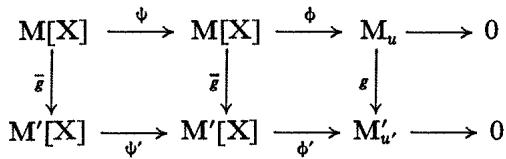
\includegraphics[keepaspectratio]{images/part004_f53e3a23.jpg}}

is commutative.

The condition \(g \circ u = u' \circ g\) is obviously necessary by (43) for \(g\) to be an A{[}X{]}-homomorphism; it is sufficient, for it implies by induction that \(g \circ u^n = u'^n \circ g\) for every integer \(n > 0\) . On the other hand, for all \(x \in M\) and all \(p \in A[X]\) ,

\[
\phi^ {\prime} (\bar {g} (p \otimes x)) = \phi^ {\prime} (p \otimes g (x)) = p (u ^ {\prime}) (g (x)) = g (p (u) (x)) = g (\phi (p \otimes x))
\]

and

\[
\bar {u} ^ {\prime} (\bar {g} (\boldsymbol {p} \otimes x)) = \bar {u} ^ {\prime} (\boldsymbol {p} \otimes g (x)) = \boldsymbol {p} \otimes u ^ {\prime} (g (x)) = \boldsymbol {p} \otimes g (u (x)) = \bar {g} (\bar {u} (\boldsymbol {p} \otimes x))
\]

which proves the commutativity of diagram (48).

\subsection{CHARACTERISTIC POLYNOMIAL OF AN ENDOMORPHISM}

Let M be a free A-module of dimension n and u an endomorphism of M. Consider the polynomial ring in two indeterminates A{[}X, Y{]} and the A{[}X, Y{]}-module M{[}X, Y{]} = A{[}X, Y{]} ⊗\_A M; let \(\bar{u}\) be the endomorphism of the A{[}X, Y{]}-module M{[}X, Y{]} canonically derived from u (II, §5, no. 1). It follows from no. 5, Proposition 11 that

\[
\det (\mathbf {X} - \mathbf {Y} \bar {\boldsymbol {u}}) = \sum_ {j = 0} ^ {n} (- 1) ^ {j} \operatorname{Tr} \left(\bigwedge^ {j} (u)\right) \mathbf {X} ^ {n - j} \mathbf {Y} ^ {j}\tag{49}
\]

for if \(U\) is the matrix of \(u\) with respect to a basis \((e_i)_{1 \leqslant i \leqslant n}\) of \(\mathbf{M}\) , \(U\) is the matrix of \(\bar{u}\) with respect to the basis \((1 \otimes e_i)_{1 \leqslant i \leqslant n}\) of \(\mathbf{M}[\mathbf{X}, \mathbf{Y}]\) , hence

\[
\operatorname{Tr} \left(\bigwedge^ {j} (\bar {u})\right) = \operatorname{Tr} \left(\bigwedge^ {j} (u)\right).
\]

DEFINITION 3. Let M be a finite-dimensional free A-module and u an endomorphism of M. The determinant of the endomorphism X - \(\bar{u}\) of the free A{[}X{]}-module M{[}X{]} is called the characteristic polynomial of u and is denoted by \(\chi_u(X)\) .

If \(\mathbf{M}\) is of rank \(n\) , it follows from (49) that

\[
\chi_ {u} (\mathbf {X}) = \sum_ {j = 0} ^ {n} (- 1) ^ {j} \operatorname{Tr} \left(\bigwedge^ {j} (u)\right) \mathbf {X} ^ {n - j}\tag{50}
\]

for \(\operatorname{det}(\mathbf{X} - \mathbf{Y}\bar{u}) = \operatorname{det}(\mathbf{X}.I_n + \mathbf{Y}U)\) and \(\operatorname{det}(\mathbf{X} - \bar{u}) = \operatorname{det}(\mathbf{X}.I_n - U)\) . It is therefore seen that \(\chi_u(\mathbf{X})\) is a monic polynomial of degree \(n\) , in which the coefficient of \(\mathbf{X}^{n-1}\) is \(-\mathrm{Tr}(u)\) and the constant term is \((-1)^n \operatorname{det}(u)\) .

PROPOSITION 20 (``Cayley-Hamilton theorem''). For every endomorphism \(u\) of a finite-dimensional free A-module, \(\chi_u(u) = 0\) .

In the notation of Proposition 18 (§ 3, no. 10), for all \(x \in \mathbf{M}\) , \(\chi_u(u)(x)\) is the image under \(\phi\) of \(\chi_u(\mathbf{X}) \otimes x\) . But if \(v\) is the endomorphism of \(\mathbf{M}[\mathbf{X}]\) , the co-transpose of \(\mathbf{X} - \bar{u}\) (no. 6), then

\[
\chi_ {u} (\mathbf {X}) \otimes x = \chi_ {u} (\mathbf {X}) (1 \otimes x) = (\mathbf {X} - \bar {u}) (v (1 \otimes x))
\]

and the conclusion follows from Proposition 18 of no. 10.

\section{NORMS AND TRACES}

Throughout this paragraph, K will denote a commutative ring and A a unital associative K-algebra. Every A-module will be assumed to be given the K-module structure obtained by restricting the scalars to K.

\subsection{NORMS AND TRACES RELATIVE TO A MODULE}

DEFINITION 1. Let M be an A-module admitting a finite basis as a K-module. For all \(a \in \mathbf{A}\) , let \(a_{\mathbf{M}}\) be the endomorphism \(x \mapsto ax\) of the K-module M. The trace, determinant and characteristic polynomial of \(a_{\mathbf{M}}\) are called respectively the trace, norm and characteristic polynomial of \(z\) relative to M.

The trace and norm of a are therefore elements of K, denoted respectively by \(\mathrm{Tr}_{\mathbf{M}/\mathbf{K}}(a)\) and \(\mathrm{N}_{\mathbf{M}/\mathbf{K}}(a)\) ; the characteristic polynomial of a is an element of K{[}X{]}, denoted by \(\mathrm{Pc}_{\mathbf{M}/\mathbf{K}}(a;\mathbf{X})\) . We omit K in the above notation when there is no risk of confusion.

From the properties of the trace and determinant of an endomorphism (II, § 4, no. 3 and § 8, no. 1) we obtain the relations

\[
\operatorname{Tr} _ {\mathbf {M}} (a + a ^ {\prime}) = \operatorname{Tr} _ {\mathbf {M}} (a) + \operatorname{Tr} _ {\mathbf {M}} (a ^ {\prime})\tag{1}
\]

\begin{enumerate}
\def\labelenumi{(\arabic{enumi})}
\setcounter{enumi}{1}
\tightlist
\item
\end{enumerate}

\[
\operatorname{Tr} _ {\mathbf {M}} (a a ^ {\prime}) = \operatorname{Tr} _ {\mathbf {M}} (a ^ {\prime} a)\tag{3}
\]

\[
\mathrm{N} _ {\mathbf {M}} (a a ^ {\prime}) = \mathrm{N} _ {\mathbf {M}} (a) \mathrm{N} _ {\mathbf {M}} (a ^ {\prime})
\]

for all \(a, a'\) in A.

Let \((e_i)_{1\leq i\leq n}\) be a basis of the K-module M and \((m_{ij}(a))\) the matrix of the endomorphism \(a_{\mathbf{M}}\) with respect to this basis. The functions \(m_{ij}\) are linear forms on the K-module A and

\begin{enumerate}
\def\labelenumi{(\arabic{enumi})}
\setcounter{enumi}{3}
\tightlist
\item
\end{enumerate}

\[
\operatorname{Tr} _ {\mathbf {M}} (a) = \sum_ {i = 1} ^ {n} m _ {i i} (a)\tag{5}
\]

\[
\mathrm{N} _ {\mathbf {M}} (a) = \det (m _ {i j} (a))\tag{6}
\]

\[
\operatorname{Pc} (a; \mathbf {X}) = \det (\delta_ {i j} \mathbf {X} - m _ {i j} (a)).
\]

It follows from the method of calculating a determinant (§ 8, no. 11, formula (50)) that

\[
\mathrm{Pc} _ {\mathbf {M}} (a; \mathbf {X}) = \mathbf {X} ^ {n} + c _ {1} \mathbf {X} ^ {n - 1} + \dots + c _ {n}\tag{7}
\]

where

\[
c _ {1} = - \operatorname{Tr} _ {\mathbf {M}} (a), \quad c _ {n} = (- 1) ^ {n} \mathrm{N} _ {\mathbf {M}} (a).\tag{8}
\]

For \(\lambda \in \mathbf{K}\) ,

\[
\operatorname{Tr} _ {\mathbf {M}} (\lambda) = n. \lambda , \quad \mathrm{N} _ {\mathbf {M}} (\lambda) = \lambda^ {n}, \quad \operatorname{Pc} _ {\mathbf {M}} (\lambda ; \mathbf {X}) = (\mathbf {X} - \lambda) ^ {n}.\tag{9}
\]

Let \(\mathbf{K}'\) be a commutative K-algebra. Let \(\mathbf{M}' = \mathbf{K}' \otimes_{\mathbf{K}} \mathbf{M}\) and \(\mathbf{A}' = \mathbf{K}' \otimes_{\mathbf{K}} \mathbf{A}\) , so that \(\mathbf{M}'\) has an A'-module structure (§ 4, Example 2). As a \(\mathbf{K}'\) -module \(\mathbf{M}'\) admits the basis consisting of the \(1 \otimes e_i\) ( \(1 \leqslant i \leqslant n\) ) and the matrix of \(a_{\mathbf{M}}\) with respect to \((e_i)\) is equal to the matrix of \((1 \otimes a)_{\mathbf{M}'}\) with respect to \((e_i')\) . Then

\[
\operatorname{Tr} _ {\mathbf {M} ^ {\prime}} (1 \otimes a) = \operatorname{Tr} _ {\mathbf {M}} (a). 1, \quad \mathrm{N} _ {\mathbf {M} ^ {\prime}} (1 \otimes a) = \mathrm{N} _ {\mathbf {M}} (a). 1\tag{12}
\]

\[
\mathrm{Pc} _ {\mathbf {M} ^ {\prime}} (1 \otimes a; \mathbf {X}) = \mathrm{Pc} _ {\mathbf {M}} (a; \mathbf {X}). 1
\]

for all \(a \in \mathbf{A}\) , where 1 denotes the unit element of \(\mathbf{K}'\) . If in particular we take \(\mathbf{K}' = \mathbf{K}[\mathbf{X}]\) , then

\[
\mathrm{Pc} _ {\mathbf {M} / \mathbf {K}} (a; \mathbf {X}) = \mathrm{N} _ {\mathbf {M} [ \mathbf {X} ] / \mathbf {K} [ \mathbf {X} ]} (\mathbf {X} - a).\tag{13}
\]

\subsection{PROPERTIES OF NORMS AND TRACES RELATIVE TO A MODULE}

If \(\mathbf{M}\) and \(\mathbf{M}'\) are two isomorphic A-modules with finite bases over \(\mathbf{K}\) , then, for all \(a \in \mathbf{A}\) ,

\[
\operatorname{Tr} _ {\mathbf {M} ^ {\prime}} (a) = \operatorname{Tr} _ {\mathbf {M}} (a), \quad \mathrm{N} _ {\mathbf {M} ^ {\prime}} (a) = \mathrm{N} _ {\mathbf {M}} (a), \quad \operatorname{Pc} _ {\mathbf {M} ^ {\prime}} (a; \mathbf {X}) = \operatorname{Pc} _ {\mathbf {M}} (a; \mathbf {X})\tag{14}
\]

for if \(f\) is an isomorphism of \(\mathbf{M}\) onto \(\mathbf{M}'\) , the matrix of \(a_{\mathbf{M}}\) with respect to a basis \(\mathbf{B}\) of \(\mathbf{M}\) over \(\mathbf{K}\) is the same as the matrix of \(a_{\mathbf{M}'}\) with respect to the basis \(f(\mathbf{B})\) of \(\mathbf{M}'\) .

PROPOSITION 1. Let \(\mathbf{M} = \mathbf{M}_0 \supset \mathbf{M}_1 \supset \cdots \supset \mathbf{M}_r = \{0\}\) be a decreasing sequence of submodules of an A-module \(\mathbf{M}\) such that each of the K-modules \(\mathbf{P}_i = \mathbf{M}_{i-1} / \mathbf{M}_i\) ( \(1 \leqslant i \leqslant r\) ) admits a finite basis. Then the K-module \(\mathbf{M}\) admits a finite basis and

\[
\operatorname{Tr} _ {\mathbf {M}} (a) = \sum_ {i = 1} ^ {r} \operatorname{Tr} _ {\mathrm{P} _ {i}} (a), \quad \mathrm{N} _ {\mathbf {M}} (a) = \prod_ {i = 1} ^ {r} \mathrm{N} _ {\mathrm{P} _ {i}} (a)\tag{15}
\]

\[
\mathrm{Pc} _ {\mathbf {M}} (a; \mathbf {X}) = \prod_ {i = 1} ^ {r} \mathrm{Pc} _ {\mathbf {P} _ {i}} (a; \mathbf {X}).
\]

Let \(B_{i}^{\prime}\) be a basis of \(P_{i}\) over K; then a system of representatives \(B_{i}\) of \(B_{i}^{\prime}\) (mod. \(M_{i}\) ) is a basis of a supplementary submodule of the K-module \(M_{i}\) in the K-module \(M_{i-1}\) (II, § 1, no. 11, Proposition 21). The union B of the \(B_{i}\) ( \(1 \leqslant i \leqslant r\) ) is a basis of M over K. Let \(X_{ii}\) be the matrix of the endomorphism \(a_{P_{i}}\) with respect to the basis \(B_{i}^{\prime}\) . It is immediate that the matrix of \(a_{M}\) with respect to B is of the form

\[
\left( \begin{array}{c c c c c} X _ {r r} & X _ {r, r - 1} & \ldots & X _ {r, 1} \\ 0 & X _ {r - 1, r - 1} & \ldots & X _ {r - 1, 1} \\ \cdot & \cdot & \cdot & \cdot & \cdot \\ 0 & 0 & \ldots & X _ {1 1} \end{array} \right)
\]

and the proposition follows from formulae (4), (5) and (6) of no. 1 and formula (31) of § 8, no. 6.

PROPOSITION 2. Let A, A' be two K-algebras, M an A-module and M' an A'-module. Suppose that M and M' are free K-modules of respective dimensions n and n' and consider M ⊗K M' as an (A ⊗K A')-module (§ 4, no. 3, Example 2). Then, for a \ensuremath{\in} A and a' \ensuremath{\in} A',

\begin{enumerate}
\def\labelenumi{(\arabic{enumi})}
\setcounter{enumi}{15}
\tightlist
\item
\end{enumerate}

\[
\operatorname{Tr} _ {\mathbf {M} \otimes \mathbf {M}} (a \otimes a ^ {\prime}) = \operatorname{Tr} _ {\mathbf {M}} (a) \operatorname{Tr} _ {\mathbf {M} ^ {\prime}} (a ^ {\prime})\tag{17}
\]

\[
\mathrm{N} _ {\mathbf {M} \otimes \mathbf {M} ^ {\prime}} (a \otimes a ^ {\prime}) = (\mathrm{N} _ {\mathbf {M}} (a)) ^ {n ^ {\prime}} (\mathrm{N} _ {\mathbf {M} ^ {\prime}} (a ^ {\prime})) ^ {n}.
\]

Formula (16) follows from II, § 4, no. 4, formula (26) and formula (17) from § 8, no. 6, formula (33).

\subsection{NORM AND TRACE IN AN ALGEBRA}

DEFINITION 2. Let A be a K-algebra which is a finite-dimensional free K-module. For every element \(a \in \mathbf{A}\) , the trace (resp. norm,† resp. characteristic polynomial) of a relative to A and K is the trace (resp. determinant, resp. characteristic polynomial) of the endomorphism \(x \mapsto ax\) of the K-module A.

The trace, norm and characteristic polynomial of \(a \in A\) relative to A and K are denoted by \(\operatorname{Tr}_{\mathbf{A}/\mathbf{K}}(a)\) , \(\operatorname{N}_{\mathbf{A}/\mathbf{K}}(a)\) and \(\operatorname{Pc}_{\mathbf{A}/\mathbf{K}}(a; \mathbf{X})\) ; we omit K and even A from this notation when there is no risk of confusion. Note that the trace (resp. norm, characteristic polynomial) of \(a \in A\) is just the trace (resp. norm, characteristic polynomial) of a relative to the A-module \(A_{s}\) .

Suppose that A is the product \(A_{1} \times A_{2} \times \cdots \times A_{m}\) of a finite number finite-dimensional algebras over K which are free K-modules. Using the above remark and Proposition 1 of no. 2, we have, for every element

\[
a = (a _ {1}, \dots , a _ {m}) \in \mathrm{A},
\]

\[
\mathrm{Tr} _ {\mathbf {A} / \mathbb {K}} (a) = \sum_ {i = 1} ^ {m} \mathrm{Tr} _ {\mathbf {A} _ {i} / \mathbb {K}} (a _ {i}), \qquad \mathrm{N} _ {\mathbf {A} / \mathbb {K}} (a) = \prod_ {i = 1} ^ {m} \mathrm{N} _ {\mathbf {A} _ {i} / \mathbb {K}} (a _ {i})\tag{18}
\]

\[
\mathrm{Pc} _ {\mathbf {A} / \mathbf {K}} (a; \mathbf {X}) = \prod_ {i = 1} ^ {m} \mathrm{Pc} _ {\mathbf {A} _ {i} / \mathbf {K}} (a _ {i}; \mathbf {X}).
\]

Similarly, Proposition 2 of no. 2 shows that if A and A' are two algebras, which are free K-modules, of finite dimensions n, \(n'\) respectively over K, then, for \(a \in A\) , \(a' \in A'\) .

\begin{enumerate}
\def\labelenumi{(\arabic{enumi})}
\setcounter{enumi}{18}
\tightlist
\item
\end{enumerate}

\[
\operatorname{Tr} _ {\mathbf {A} \otimes \mathbf {A} ^ {\prime}} (a \otimes a ^ {\prime}) = \operatorname{Tr} _ {\mathbf {A}} (a) \operatorname{Tr} _ {\mathbf {A} ^ {\prime}} (a ^ {\prime})\tag{20}
\]

\[
\mathrm{N} _ {\mathbf {A} \otimes \mathbf {A} ^ {\prime}} (a \otimes a ^ {\prime}) = (\mathrm{N} _ {\mathbf {A}} (a)) ^ {n ^ {\prime}} (\mathrm{N} _ {\mathbf {A} ^ {\prime}} (a ^ {\prime})) ^ {n}.
\]

Finally let A be a finite-dimensional algebra over K which is a free K-module, h a homomorphism of K into a commutative ring \(K'\) and \(A' = A_{(K')}\) the \(K'\) -algebra derived from A by extending the scalars by means of h. It follows from formula (12) of no. 1 that, for all \(a \in A\) ,

\[
\begin{array}{r l} \mathrm{Tr} _ {\mathbf {A} ^ {\prime} / \mathbf {K} ^ {\prime}} (1 \otimes a) & = h (\mathrm{Tr} _ {\mathbf {A} / \mathbf {K}} (a)), \quad \mathrm{N} _ {\mathbf {A} ^ {\prime} / \mathbf {K} ^ {\prime}} (1 \otimes a) = h (\mathrm{N} _ {\mathbf {A} / \mathbf {K}} (a)) \\ \mathrm{Pc} _ {\mathbf {A} ^ {\prime} / \mathbf {K} ^ {\prime}} (1 \otimes a; \mathbf {X}) & = \tilde {h} (\mathrm{Pc} _ {\mathbf {A} / \mathbf {K}} (a; \mathbf {X})) \end{array}\tag{21}
\]

where \(\tilde{h}\) is the homomorphism \(\mathbf{K}[\mathbf{X}] \to \mathbf{K}'[\mathbf{X}]\) derived from \(h\) . In particular, for \(\mathbf{K}' = \mathbf{K}[\mathbf{X}]\) , we obtain, writing \(\mathrm{A}[\mathbf{X}] = \mathrm{A} \otimes_{\mathbf{K}} \mathbf{K}[\mathbf{X}]\) ,

\[
\mathrm{Pc} _ {\mathbf {A} / \mathbf {K}} (a; \mathbf {X}) = \mathrm{N} _ {\mathbf {A} [ \mathbf {X} ] / \mathbf {K} [ \mathbf {X} ]} (\mathbf {X} - a).\tag{22}
\]

More generally, if \(\mathbf{K}'\) is a commutative \(\mathbf{K}\) -algebra and \(\mathbf{A}' = \mathbf{A} \otimes_{\mathbf{K}} \mathbf{K}'\) , then, for all \(x \in \mathbf{A}'\) ,

\[
\mathrm{Pc} _ {\mathbf {A} / \mathbf {K}} (a; x) = \mathrm{N} _ {\mathbf {A} ^ {\prime} / \mathbf {K} ^ {\prime}} (x - a).
\]

Examples. (1) Let A be a quadratic algebra over K of type \((\alpha, \beta)\) and \((e_1, e_2)\) a basis of type \((\alpha, \beta)\) (§ 2, no. 3). For \(x = \xi e_1 + \eta e_2\) , \(\operatorname{Tr}_{A/K}(x) = 2\xi + \beta \eta\) and \(\mathrm{N}_{A/K}(x) = \xi^2 + \beta \xi \eta - \alpha \eta^2\) ; these functions are therefore identical with the Cayley trace and norm of \(x\) (§ 2, no. 24).

\begin{enumerate}
\def\labelenumi{(\arabic{enumi})}
\setcounter{enumi}{1}
\item
  Let A be a quaternion algebra over K. A direct calculation allows us to verify that \(\mathrm{Tr}_{\mathbf{A} / \mathbb{K}}(x) = 2\mathrm{T}(x)\) and \(\mathrm{N}_{\mathbf{A} / \mathbb{K}}(x) = (\mathrm{N}(x))^2\) , where \(\mathbf{T}\) and \(\mathbf{N}\) are the Cayley trace and norm (§ 2, no. 4).
\item
  Let \(\mathbf{A} = \mathbf{M}_n(\mathbf{K})\) and let the canonical basis \((E_{ij})\) of \(\mathbf{A}\) (II, § 10, no. 3) be arranged in lexicographic order. Then it is immediately seen that for every matrix \(\mathbf{X} = \sum_{i,j} \xi_{ij} E_{ij}\) the matrix (of order \(n^2\) ) of the endomorphism \(Y \mapsto XY\) is of the form
\end{enumerate}

\[
\left( \begin{array}{c c c c} X & 0 & \ldots & 0 \\ 0 & X & \ldots & 0 \\ . & . & . & . \\ 0 & 0 & \ldots & X \end{array} \right)
\]

whence \(\operatorname{Tr}_{\mathbf{A} / \mathbb{K}}(X) = n.\operatorname{Tr}(X)\) and \(\mathrm{N}_{\mathbf{A} / \mathbb{K}}(X) = (\det (X))^n\)

\subsection{PROPERTIES OF NORMS AND TRACES IN AN ALGEBRA}

PROPOSITION 3. Let A be a K-algebra admitting a finite basis. For an element \(a \in \mathbf{A}\) to be invertible, it is necessary and sufficient that its \(\mathbf{N}_{\mathbf{A} / \mathbf{K}}(a)\) be invertible in \(\mathbf{K}\) .

If \(a\) admits an inverse \(a'\) in \(\mathbf{A}\) , then

\[
\mathrm{N} _ {\mathbf {A} / \mathbf {K}} (a) \mathrm{N} _ {\mathbf {A} / \mathbf {K}} (a ^ {\prime}) = \mathrm{N} _ {\mathbf {A} / \mathbf {K}} (a a ^ {\prime}) = \mathrm{N} _ {\mathbf {A} / \mathbf {K}} (1) = 1
\]

by formula (3) of no. 1. Conversely, if \(\mathbf{N}_{\mathbf{A} / \mathbb{K}}(a)\) is invertible, the endomorphism \(h: x \mapsto ax\) is bijective (§ 8, no. 2, Theorem 1). Then there exists \(a' \in A\) such that \(aa' = 1\) ; then \(h(a'a - 1) = aa'a - a = (aa' - 1)a = 0\) , whence \(aa' = 1\) since \(h\) is injective. Hence \(a'\) is the inverse of \(a\) .

PROPOSITION 4. Let A be a K-algebra admitting a finite basis. For all \(a \in \mathbf{A}\) , \(\operatorname{Pc}_{\mathbf{A} / \mathbf{K}}(a; a) = 0\) .

This follows immediately from the Cayley-Hamilton theorem (§ 8, no. 11, Proposition 20).

PROPOSITION 5. Let A be a K-algebra and m a two-sided ideal of A. Suppose that \(A_{0} = A/m\) is a free K-module of finite dimension n, that there exists an integer r \textgreater{} 0 such that \(m^{r} = \{0\}\) and that \(m^{i-1}/m^{i}\) is a free \(A_{0}\) -module of finite dimension \(s_{i}\) for \(1 \leqslant i \leqslant r\) . Let \(s = s_{1} + \cdots + s_{r}\) and for all \(a \in A\) let \(a_{0}\) denote the class of a mod. m. Then A is a free K-module of dimension ns and, for all \(a \in A\) ,

\[
\operatorname{Tr} _ {\mathbf {A}} (a) = s. \operatorname{Tr} _ {\mathbf {A} _ {0}} (a _ {0}), \quad \mathrm{N} _ {\mathbf {A}} (a) = (\mathrm{N} _ {\mathbf {A} _ {0}} (a _ {0})) ^ {s}\tag{23}
\]

\[
\mathrm{Pc} _ {\mathbf {A}} (a; \mathbf {X}) = (\mathrm{Pc} _ {\mathbf {A} _ {0}} (a _ {0}; \mathbf {X})) ^ {s}.
\]

By virtue of II, § 1, no. 13, Proposition 25, \(\mathfrak{m}^{i - 1} / \mathfrak{m}^{i}\) is a free K-module of dimension \(ns_i\) . Hence Proposition 1 of no. 2 can be applied with \(\mathbf{P}_i = \mathfrak{m}^{i - 1} / \mathfrak{m}^{i}\) ;

this shows in the first place that A is a free K-module of dimension \(n(s_{1} + \cdots + s_{r}) = ns\) . Moreover, the hypothesis implies that the A-module \(P_{i}\) is isomorphic to a direct sum of \(s_{i}\) submodules isomorphic to the A-module \(A_{0}\) ; by Proposition 1 of no. 2, therefore \(\mathrm{N}_{\mathrm{P}_{i}}(a) = \mathrm{N}_{\mathrm{A}_{0}}(a)^{s_{i}}\) ; finally therefore

\[
\mathrm{N} _ {\mathbf {A}} (a) = \mathrm{N} _ {\mathbf {A} _ {0}} (a) ^ {s}.
\]

In this formula \(\mathrm{N}_{\mathbf{A}_{0}}(a)\) is defined by considering \(A_{0}\) as a left A-module and it is equal to the determinant of the K-linear mapping \(x \mapsto ax\) of \(A_{0}\) into itself; but, as \(ax = a_{0}x\) for \(x \in A_{0}\) , \(\mathrm{N}_{\mathbf{A}_{0}}(a) = \mathrm{N}_{\mathbf{A}_{0}}(a_{0})\) , which completes the proof of formula (23) for the norm. The two others are shown analogously.

PROPOSITION 6. Let A be a commutative K-algebra admitting a finite basis over K and V an A-module admitting a finite basis over A. Then V admits a finite basis over K and for every A-endomorphism u of V, if \(u_{\mathbf{K}}\) is the mapping u considered as a K-endomorphism of V,

\[
\operatorname{Tr} (u _ {\mathbb {K}}) = \operatorname{Tr} _ {\mathbf {A} / \mathbb {K}} (\operatorname{Tr} (u)), \quad \det (u _ {\mathbb {K}}) = \mathrm{N} _ {\mathbf {A} / \mathbb {K}} (\det (u))\tag{24}
\]

\[
\operatorname{Pc} (u _ {\mathbf {K}}; \mathbf {X}) = \mathrm{N} _ {\mathbf {A} [ \mathbf {X} ] / \mathbf {K} [ \mathbf {X} ]} (\operatorname{Pc} (u; \mathbf {X})).
\]

Let \((a_{i})_{1\leqslant i\leqslant m}\) be a basis of A over K and \((e_{j})_{1\leqslant j\leqslant n}\) a basis of V over A; then \((a_{i}e_{j})\) is a basis of V over K (II, § 1, no. 13, Proposition 25). On the other hand the third of formulae (24) can be deduced from the second applied to the endomorphism \(\mathbf{X} - \bar{\boldsymbol{u}}\) of the A{[}X{]}-module A{[}X{]} \(\otimes_{\mathbf{A}}\mathrm{V}\) (§ 8, no. 10). It will therefore suffice to show the first two formulae in (24). We shall first establish the following lemma:

Lemma 1. Let \(\mathbf{X}_{ij}\) ( \(1 \leqslant i \leqslant n\) , \(1 \leqslant j \leqslant n\) ) be \(n^2\) indeterminates, \(X\) the square matrix \((\mathbf{X}_{ij})\) of order \(n\) and \(\mathbf{D}(\mathbf{X}_{11}, \ldots, \mathbf{X}_{nn}) \in \mathbf{Z}[\mathbf{X}_{11}, \ldots, \mathbf{X}_{nn}]\) the determinant \(\det(X)\) . On the other hand let A be a commutative ring, \(\mathbf{M}_{ij}\) ( \(1 \leqslant i \leqslant n\) , \(1 \leqslant j \leqslant n\) ) \(n^2\) matrices of order \(m\) over A, which are pairwise permutable, and M the square matrix of order \(mn\) over A which can be expressed as a square matrix of matrices (II, § 10, no. 7)

\[
M = \left( \begin{array}{c c c c} M _ {1 1} & M _ {1 2} & \ldots & M _ {1 n} \\ M _ {2 1} & M _ {2 2} & \ldots & M _ {2 n} \\ \cdot & \cdot & \cdot & \cdot \\ M _ {n 1} & M _ {n 2} & \ldots & M _ {n n} \end{array} \right)
\]

Then the determinant of M is equal to the determinant of the square matrix

\[
\mathrm{D} (M _ {1 1}, \dots , M _ {n n})
\]

of order m.

We proceed by induction on \(n\) , the cases \(n = 0\) and \(n = 1\) being trivial.

Let \(Z\) be a new indeterminate and \(N_{ij}\) the matrix \(M_{ij} + \delta_{ij}ZI_m\) ( \(\delta_{ij}\) the Kronecker index). If \(D^{ij}(X_{11},\ldots,X_{nn})\) is the cofactor of \(X_{ij}\) in the matrix \(X\) (§ 8, no. 6), then

\[
\mathrm{X} _ {j l} \mathrm{D} ^ {k l} (\mathrm{X} _ {1 1}, \dots , \mathrm{X} _ {n n}) = \delta_ {j k} \mathrm{D} (\mathrm{X} _ {1 1}, \dots , \mathrm{X} _ {n n})\tag{25}
\]

(§ 8, no. 6, formula (28)). We write \(N_{ij}' = \mathbf{D}^{ij}(N_{11}, \ldots, N_{nn})\) , which is a square matrix of order \(m\) over \(\mathrm{A}[Z]\) and consider the product \(N.U\) , where

\[
U = \left( \begin{array}{c c c c} N _ {1 1} ^ {\prime} & 0 & \ldots & 0 \\ N _ {1 2} ^ {\prime} & I _ {m} & \ldots & 0 \\ \cdot & \cdot & \cdot & \cdot \\ N _ {1 n} ^ {\prime} & 0 & \ldots & I _ {m} \end{array} \right),
\]

\[
N = \left( \begin{array}{c c c c} N _ {1 1} & N _ {1 2} & \ldots & N _ {1 n} \\ N _ {2 1} & N _ {2 2} & \ldots & N _ {2 n} \\ \cdot & \cdot & \cdot & \cdot \\ N _ {n 1} & N _ {n 2} & \ldots & N _ {n n} \end{array} \right)
\]

Performing this product in blocks (II, § 10, no. 5) and using formulae (25), we obtain

\[
N. U = \left( \begin{array}{c c c c} P & N _ {1 2} & \ldots & N _ {1 n} \\ 0 & N _ {2 2} & \ldots & N _ {2 n} \\ \cdot & \cdot & \cdot & \cdot \\ 0 & N _ {n 2} & \ldots & N _ {n n} \end{array} \right)
\]

where we have written \(P = \mathrm{D}(N_{11},\ldots ,N_{nn})\) .Let

\[
Q = \left( \begin{array}{c c c c} N _ {2 2} & \ldots & N _ {2 n} \\ \cdot & \cdot & \cdot & \cdot \\ N _ {n 2} & \ldots & N _ {n n} \end{array} \right)
\]

which is a matrix of order \(m(n - 1)\) ; then (§8, no. 6, formula (31)) (det \(N\) ) ( \(\det U\) ) = ( \(\det P\) ) ( \(\det Q\) ) and \(\det U = \det N_{11}'\) . But by the induction hypothesis, \(\det Q = \det(\mathrm{D}^{11}(N_{11},\ldots ,N_{nn})) = \det N_{11}'\) and by virtue of the definition of the \(N_{ij}\) , clearly \(\det Q\) is a polynomial in A{[}Z{]} of degree \(m(n - 1)\) , whose term in \(Z^{m(n - 1)}\) has coefficient 1; it follows immediately that \(\det Q\) is not a divisor of zero in the graded algebra A{[}Z{]}. We therefore conclude that \(\det N = \det(\mathrm{D}(N_{11},\ldots ,N_{nn}))\) in A{[}Z{]}; if we substitute 0 for Z in these polynomials, then \(\det M = \det(\mathrm{D}(M_{11},\ldots ,M_{nn}))\) .

Having shown this lemma, the K-module V is the direct sum of the K-modules \(Ae_{j}\) ( \(1 \leqslant j \leqslant n\) ); we write \(u(e_{j}) = \sum_{k=1}^{n} c_{jk} e_{k}\) . For every element \(xe_{j} \in Ae_{j}\) , with \(x \in A\) , the component of \(u(xe_{j})\) in \(Ae_{k}\) is \(xc_{jk} e_{k}\) ; it follows that the matrix of \(u_{k}\) with respect to the basis \((a_{i} e_{j})\) of the K-module V can be expressed in the form of a square matrix of matrices \((M_{jk})\) , where \(M_{jk}\) is the matrix of the K-linear mapping \(xe_{j} \mapsto xc_{jk} e_{k}\) of \(Ae_{j}\) into \(Ae_{k}\) with respect to the bases \((a_{i} e_{j})_{1 \leqslant i \leqslant m}\) and \((a_{i} e_{k})_{1 \leqslant i \leqslant m}\) of these two K-modules (II, § 10, no. 5). If for all \(t \in A\) , \(M(t)\) denotes the matrix, with respect to the basis \((a_{i})_{1 \leqslant i \leqslant m}\) of A over K, of the endomorphism \(x \mapsto xt\) of A, then \(M_{jk} = M(c_{jk})\) ; as \(t \mapsto M(t)\) is a ring homomorphism the matrices \(M_{jk}\) are permutable with one another. Then

\[
\det u _ {\mathrm{K}} = \det (\mathrm{D} (M _ {1 1}, \dots , M _ {n n}))
\]

by Lemma 1. But as \(t \mapsto M(t)\) is a ring homomorphism, \(\mathrm{D}(M_{11},\ldots ,M_{nn})\) is the matrix of the K-endomorphism \(x \mapsto x.\det (c_{jk})\) of A with respect to basis \((a_t)\) ; by definition its determinant is therefore \(\mathrm{N}_{\mathbf{A} / \mathbf{K}}(\det (u))\) , which proves the second formula of (24). On the other hand,

\[
\operatorname{Tr} \left(u _ {\mathrm{K}}\right) = \sum_ {j = 1} ^ {n} \operatorname{Tr} \left(M _ {j j}\right) = \sum_ {j = 1} ^ {n} \operatorname{Tr} _ {\mathrm{A} / \mathrm{K}} \left(c _ {j j}\right) = \operatorname{Tr} _ {\mathrm{A} / \mathrm{K}} \left(\sum_ {j = 1} ^ {n} c _ {j j}\right) = \operatorname{Tr} _ {\mathrm{A} / \mathrm{K}} (\operatorname{Tr} (u))
\]

and the proof of Proposition 6 is complete.

COROLLARY. Let A be a commutative K-algebra admitting a finite basis over K and B an A-algebra admitting a finite basis over A. Then B admits a finite basis over K, and, for all \(b \in B\) (``transitivity formulae'')

\[
\operatorname{Tr} _ {\mathbf {B} / \mathbf {K}} (b) = \operatorname{Tr} _ {\mathbf {A} / \mathbf {K}} (\operatorname{Tr} _ {\mathbf {B} / \mathbf {A}} (b)), \quad \mathrm{N} _ {\mathbf {B} / \mathbf {K}} (b) = \mathrm{N} _ {\mathbf {A} / \mathbf {K}} (\mathrm{N} _ {\mathbf {B} / \mathbf {A}} (b))\tag{26}
\]

\[
\mathrm{Pc} _ {\mathbf {B} / \mathbf {K}} (b; \mathbf {X}) = \mathrm{N} _ {\mathbf {A} [ \mathbf {X} ] / \mathbf {K} [ \mathbf {X} ]} (\mathrm{Pc} _ {\mathbf {B} / \mathbf {A}} (b; \mathbf {X})).
\]

This follows immediately from Proposition 6, setting \(\mathbf{V} = \mathbf{B}\) and \(u(x) = bx\) .

Remark. Suppose that the homomorphism \(\lambda \mapsto \lambda, 1\) of K into A is injective and let K be identified with its image in A; suppose that A admits a finite basis \((e_i)_{1 \leqslant i \leqslant n}\) as a K-module. Let \(s\) be an automorphism of A such that \(s(\mathbf{K}) = \mathbf{K}\) . Let \(a\) be an element of A; then, by transporting the structure

\begin{enumerate}
\def\labelenumi{(\arabic{enumi})}
\setcounter{enumi}{26}
\tightlist
\item
\end{enumerate}

\[
\operatorname{Tr} _ {\mathbf {A} / \mathbf {K}} (s (a)) = s (\operatorname{Tr} _ {\mathbf {A} / \mathbf {K}} (a))\tag{28}
\]

\[
\mathrm{N} _ {\mathbf {A} / \mathbf {K}} (s (a)) = s (\mathrm{N} _ {\mathbf {A} / \mathbf {K}} (a)).
\]

*Consider also a derivation D of A (§ 10, no. 2) such that D(K) ⊂ K and write \(D (e _ {i}) = \sum_ {j = 1} ^ {n} e _ {j} \mu_ {j i}\) where \(\mu_ {j i} \in \mathbf {K}\); write

\[
a e _ {i} = \sum_ {j = 1} ^ {n} e _ {j} \lambda_ {j i} \quad \text { with } \quad \lambda_ {j i} \in \mathbf {K}.
\]

Then

\[
\mathrm{D} (a) e _ {i} + a \mathrm{D} (e _ {i}) = \mathrm{D} (a e _ {i}) = \sum_ {j = 1} ^ {n} (\mathrm{D} (e _ {j}) \lambda_ {j i} + e _ {j} \mathrm{D} (\lambda_ {j i})).
\]

It follows that

\[
\mathbf {D} (a) e _ {i} = \sum_ {j = 1} ^ {n} e _ {j} \nu_ {j i}
\]

with \(\nu_{ji} = \mathrm{D}(\lambda_{ji}) + \sum_{k=1}^{n} (\mu_{jk}\lambda_{ki} - \lambda_{jk}\mu_{ki})\) . As \(\sum_{i,k} (\mu_{ik}\lambda_{ki} - \lambda_{ik}\mu_{ki}) = 0\) , there-

fore \(\mathrm{Tr}_{\mathbf{A} / \mathbb{K}}(\mathbf{D}(a)) = \sum_{i = 1}^{n}\mathbf{D}(\lambda_{ii})\) , in other words

\[
\operatorname{Tr} _ {\mathbf {A} / \mathbf {K}} (\mathbf {D} (a)) = \mathbf {D} (\operatorname{Tr} _ {\mathbf {A} / \mathbf {K}} (a)). *\tag{29}
\]

\subsection{DISCRIMINANT OF AN ALGEBRA}

DEFINITION 3. Let A be a K-algebra admitting a finite basis of n elements. The discriminant of a sequence \((x_{1},\ldots,x_{n})\) of n elements of A, with respect to K, denoted by \(\mathrm{D}_{\mathrm{A}/\mathrm{K}}(x_{1},\ldots,x_{n})\) , is the discriminant of the square matrix

\[
\left(\operatorname{Tr} _ {\mathbf {A} / \mathbb {K}} \left(x _ {i} x _ {j}\right)\right) _ {1 \leqslant i \leqslant n, 1 \leqslant j \leqslant n}.
\]

Consider first a basis \((e_i)_{1\leqslant i\leqslant n}\) of A over K and write

\[
e _ {i} e _ {j} = \sum_ {k = 1} ^ {n} c _ {i j k} e _ {k} \quad \text { with } \quad c _ {i j k} \in \mathbf {K}.\tag{30}
\]

Then \(\mathrm{Tr}_{\mathbf{A} / \mathbf{K}}(e_i) = \sum_{s=1}^{n} c_{iss}\) , whence \(\mathrm{Tr}_{\mathbf{A} / \mathbf{K}}(e_i e_j) = \sum_{k,s} c_{ijk} c_{kss}\) and therefore

\[
\mathrm{D} _ {\mathrm{A} / \mathrm{K}} (e _ {1}, \dots , e _ {n}) = \det \left(\left(\sum_ {k, s} c _ {i j k} c _ {k s s}\right) _ {1 \leqslant i \leqslant n, 1 \leqslant j \leqslant n}\right).\tag{31}
\]

Now let \((x_{i})_{1\leqslant i\leqslant n},(x_{i}^{\prime})_{1\leqslant i\leqslant n}\) be two sequences of \(n\) elements of A and suppose that there exists a square matrix of order \(n\) , \(M = (m_{ij})\) , with coefficients in K, such that \(x_{i} = \sum_{j=1}^{n} m_{ij} x_{j}'\) for \(1 \leqslant i \leqslant n\) . We write

\[
T = \left(\operatorname{Tr} _ {\mathrm{A} / \mathrm{K}} \left(x _ {i} x _ {j}\right)\right) _ {1 \leqslant i \leqslant n, 1 \leqslant j \leqslant n}, \quad T ^ {\prime} = \left(\operatorname{Tr} _ {\mathrm{A} / \mathrm{K}} \left(x _ {i} ^ {\prime} x _ {j} ^ {\prime}\right)\right) _ {1 \leqslant i \leqslant n, 1 \leqslant j \leqslant n}.
\]

Then \(\mathrm{Tr}_{\mathbf{A} / \mathbf{K}}(x_i x_j) = \sum_{p,q} m_{ip} m_{jq} \mathrm{Tr}_{\mathbf{A} / \mathbf{K}}(x_p' x_q')\) , whence \(T = M. T'.^t M\) ; the rule of multiplication of determinants therefore gives

\[
\det T = \det M. \det T ^ {\prime}. \det ^ {t} M = (\det M) ^ {2} \det T ^ {\prime}
\]

whence finally

\[
\mathrm{D} _ {\mathrm{A} / \mathrm{K}} (x _ {1}, \dots , x _ {n}) = (\det M) ^ {2} \mathrm{D} _ {\mathrm{A} / \mathrm{K}} (x _ {i} ^ {\prime}, \dots , x _ {n} ^ {\prime}).\tag{32}
\]

The above formula shows in particular that the discriminants of two bases of A over K differ by the square of an invertible element of K and therefore generate the same (principal) ideal of K. This ideal \(\Delta_{A/K}\) is called the discriminant ideal of A over K; by formula (32) the discriminant of every sequence of n elements of A which differ only in the order of the terms have the same discriminant, for the determinant of a permutation matrix is equal to \(\pm1\) .

Examples. (1) If A is a quadratic algebra of type \((\alpha, \beta)\) over K, then (in the notation of §2, no. 3) \(\operatorname{Tr}(e_1) = 2\) , \(\operatorname{Tr}(e_2) = \beta\) ,

\[
\operatorname{Tr} (e _ {2} ^ {2}) = \alpha \operatorname{Tr} (e _ {1}) + \beta \operatorname{Tr} (e _ {2}) = 2 \alpha + \beta^ {2},
\]

whence \(\mathbf{D}_{\mathbf{A} / \mathbb{K}}(e_1,e_2) = \beta^2 +4\alpha .\)

\begin{enumerate}
\def\labelenumi{(\arabic{enumi})}
\setcounter{enumi}{1}
\item
  Let \(\mathbf{A} = \mathbf{K}[\mathbf{X}] / \mathbf{K}[\mathbf{X}]\mathbf{P}\) , where \(\mathrm{P}(\mathbf{X}) = \mathbf{X}^3 + p\mathbf{X} + q\) , so that if \(x\) is the image of \(\mathbf{X}\) in \(\mathbf{A}, 1, x, x^2\) form a basis of \(\mathbf{A}\) over \(\mathbf{K}\) and \(x^3 = -px - q\) . It is seen immediately that \(\operatorname{Tr}(1) = 3\) , \(\operatorname{Tr}(x) = 0\) , \(\operatorname{Tr}(x^2) = -2p\) , taking account of the relation \(x^3 = -px - q\) , \(\operatorname{Tr}(x^3) = -3q\) and \(\operatorname{Tr}(x^4) = 2p^2\) , whence easily \(\mathrm{D}_{\mathbf{A} / \mathbf{K}}(1, x, x^2) = -4p^3 - 27q^2\) .
\item
  Let A be a quaternion algebra of type \((\alpha, \beta, \gamma)\) over K and \((1, i, j, k)\) a basis of A of type \((\alpha, \beta, \gamma)\) ; taking account of § 3, no. 5, formula (30), it is easily found that \(\operatorname{Tr}(1) = 4\) , \(\operatorname{Tr}(i) = 2\beta\) , \(\operatorname{Tr}(j) = \operatorname{Tr}(k) = 0\) , then
\end{enumerate}

\[
\mathrm{D} _ {\mathrm{A/K}} (1, i, j, k) = - 16 \gamma^ {2} (\beta^ {2} + 4 \alpha) ^ {2}.
\]

\begin{enumerate}
\def\labelenumi{(\arabic{enumi})}
\setcounter{enumi}{3}
\tightlist
\item
  Let \(\mathbf{A} = \mathbf{M}_n(\mathbf{K})\) and consider the canonical basis \((E_{ij})_{1\leqslant i\leqslant n,1\leqslant j\leqslant n}\) of \(\mathbf{A}\) over \(\mathbf{K}\) (II, § 10, no. 3). It is immediate that \(\operatorname{Tr}_{\mathbf{A} / \mathbf{K}}(E_{ij}) = 0\) if \(j\neq i\) and \(\operatorname{Tr}_{\mathbf{A} / \mathbf{K}}(E_{ii}) = n\) for all \(i\) ; it follows without difficulty that the matrix \((\operatorname{Tr}(E_{ij}E_{hk}))\) of order \(n^2\) is of the form \(n.P\) , where \(P\) is a permutation matrix, whence \(\mathrm{D}_{\mathbf{A} / \mathbf{K}}((E_{ij})) = \pm n^{n^2}\) .
\end{enumerate}

\section{DERIVATIONS}

In this paragraph, and unless otherwise mentioned, the algebras considered are not assumed to be associative nor necessarily to possess a unit element; K denotes a commutative ring.

\subsection{COMMUTATION FACTORS}

When in this paragraph we speak of graduations without specifying them, we shall always mean graduations of type \(\Delta\) , where \(\Delta\) is a commutative group written additively. In this paragraph, a commutation factor over \(\Delta\) with values in Z is called a commutation factor over \(\Delta\) ( \(\S\) 4, no. 7, Definition 6). A commutation factor over \(\Delta\) is therefore identified with a mapping \(\varepsilon\colon(\alpha,\beta)\mapsto\varepsilon_{\alpha\beta}=\varepsilon(\alpha,\beta)\) of \(\Delta\times\Delta\) into the multiplicative group \(\{-1,1\}\) such that for \(\alpha,\alpha^{\prime},\beta,\beta^{\prime}\) in \(\Delta\) ,

\[
\left\{ \begin{array}{l} \varepsilon (\alpha + \alpha^ {\prime}, \beta) = \varepsilon (\alpha , \beta) \varepsilon (\alpha^ {\prime}, \beta) \\ \varepsilon (\alpha , \beta + \beta^ {\prime}) = \varepsilon (\alpha , \beta) \varepsilon (\alpha , \beta^ {\prime}) \\ \varepsilon (\beta , \alpha) = \varepsilon (\alpha , \beta). \end{array} \right.\tag{1}
\]

It follows that \(\varepsilon(2\alpha, \beta) = \varepsilon(\alpha, 2\beta) = 1\) .

When \(\Delta = \mathbf{Z}\) , every commutation factor \(\varepsilon\) is determined by giving \(\varepsilon(1, 1)\) ; there are therefore only two such factors, the first defined by

\[
\varepsilon (p, q) = 1 \quad \text { for } \quad p, q \text { in } \mathbf {Z}\tag{2}
\]

and the second by

\[
\varepsilon (p, q) = (- 1) ^ {p q} \quad \text { for } \quad p, q \text { in } \mathbf {Z}.\tag{3}
\]

\subsection{GENERAL DEFINITION OF DERIVATIONS}

Consider a commutative ring K, six graded K-modules of type \(\Delta\) : A, A', A'', B, B', B'', and three K-linear mappings

\[
\mu \colon \mathrm{A} \times \mathrm{A} ^ {\prime} \rightarrow \mathrm{A} ^ {\prime \prime}, \quad \lambda_ {1} \colon \mathrm{B} \times \mathrm{A} ^ {\prime} \rightarrow \mathrm{B} ^ {\prime \prime}, \quad \lambda_ {2} \colon \mathrm{A} \times \mathrm{B} ^ {\prime} \rightarrow \mathrm{B} ^ {\prime \prime}
\]

such that the corresponding K-linear mappings

\[
\mathrm{A} \otimes_ {\mathrm{K}} \mathrm{A} ^ {\prime} \rightarrow \mathrm{A} ^ {\prime \prime}, \quad \mathrm{B} \otimes_ {\mathrm{K}} \mathrm{A} ^ {\prime} \rightarrow \mathrm{B} ^ {\prime \prime}, \quad \mathrm{A} \otimes_ {\mathrm{K}} \mathrm{B} ^ {\prime} \rightarrow \mathrm{B} ^ {\prime \prime}
\]

are graded of degree 0. The image \(\mu(a, a')\) for \(a \in A\) , \(a' \in A'\) is simply denoted by \(a, a'\) or even \(aa'\) , and similarly for the two other bilinear mappings. The degree of \(a, a'\) is therefore the sum of the degrees of \(a\) and \(a'\) .

DEFINITION 1. Given the above and a commutation factor \(\varepsilon\) on \(\Delta \times \Delta\) , an \(\varepsilon\) -derivation (or \((\mathbf{K}, \varepsilon)\) -derivation) of degree \(\delta \in \Delta\) of \((\mathbf{A}, \mathbf{A}', \mathbf{A}'')\) into \((\mathbf{B}, \mathbf{B}', \mathbf{B}'')\) is a triple of graded K-linear mappings of degree \(\delta\) :

\[
d \colon \mathrm{A} \rightarrow \mathrm{B}, \quad d ^ {\prime} \colon \mathrm{A} ^ {\prime} \rightarrow \mathrm{B} ^ {\prime}, \quad d ^ {\prime \prime} \colon \mathrm{A} ^ {\prime \prime} \rightarrow \mathrm{B} ^ {\prime \prime}
\]

such that, for every homogeneous element \(a \in A\) and every element \(a' \in A'\)

\[
d ^ {\prime \prime} (a. a ^ {\prime}) = (d a). a ^ {\prime} + \varepsilon_ {\delta , \deg (a)} a. (d ^ {\prime} a ^ {\prime}).\tag{4}
\]

It obviously suffices by linearity to verify relation (4) when \(a\) and \(a'\) run through respective generating systems of A and A'.

It is often convenient to denote the three mappings \(d, d', d''\) by the same letter \(d\) (which can be justified by denoting equally by \(d\) the graded K-linear mapping of degree \(\delta\) )

\[
(a, a ^ {\prime}, a ^ {\prime \prime}) \mapsto (d a, d ^ {\prime} a ^ {\prime}, d ^ {\prime \prime} a ^ {\prime \prime})
\]

of \(\mathbf{A} \oplus \mathbf{A}' \oplus \mathbf{A}''\) into \(\mathbf{B} \oplus \mathbf{B}' \oplus \mathbf{B}''\) . Relation (4) can then be written more simply

\[
d (a. a ^ {\prime}) = (d a). a ^ {\prime} + \varepsilon_ {\delta . \deg (a)} a. (d a ^ {\prime}).\tag{5}
\]

The \(\varepsilon\) -derivations of (A, A', A'') into (B, B', B'') of given degree form a sub-K-module of the K-module of graded linear mappings

\[
\operatorname{Homgr} _ {\mathbb {K}} (\mathrm{A} \oplus \mathrm{A} ^ {\prime} \oplus \mathrm{A} ^ {\prime \prime}, \mathrm{B} \oplus \mathrm{B} ^ {\prime} \oplus \mathrm{B} ^ {\prime \prime}).
\]

When \(\varepsilon(\alpha, \beta) = 1\) for all \(\alpha, \beta\) in \(\Delta\) , we say simply derivation (or K-derivation) instead of \(\varepsilon\) -derivation. Derivations form a sub-K-module of

\[
\operatorname{Hom} _ {\mathbb {K}} (\mathrm{A} \oplus \mathrm{A} ^ {\prime} \oplus \mathrm{A} ^ {\prime \prime}, \mathrm{B} \oplus \mathrm{B} ^ {\prime} \oplus \mathrm{B} ^ {\prime \prime}).
\]

When \(\Delta = Z\) and \(\varepsilon(p, q) = (-1)^{pq}\) , every \(\varepsilon\) -derivation of even degree is a derivation; every \(\varepsilon\) -derivation of odd degree is often called an antiderivation (or K-antiderivation); an antiderivation d therefore satisfies

\[
d (a. a ^ {\prime}) = (d a). a ^ {\prime} + (- 1) ^ {\deg (a)} a. (d a ^ {\prime})\tag{6}
\]

for a homogeneous element \(a \in A\) .

Remarks. (1) The notion of derivation can be defined for non-graded modules by agreeing to give these modules the trivial graduation.

\begin{enumerate}
\def\labelenumi{(\arabic{enumi})}
\setcounter{enumi}{1}
\tightlist
\item
  If only \(\varepsilon\) -derivations of given degree \(\delta\) are considered, the commutation factor \(\varepsilon\) may be disposed of as follows: the bilinear mapping \(\lambda_2: \mathbf{A} \times \mathbf{B}' \to \mathbf{B}''\) is modified by replacing it by the bilinear mapping \(\lambda_2': \mathbf{A} \times \mathbf{B}' \to \mathbf{B}''\) such that, for every homogeneous \(a\) in \(\mathbf{A}\) and all \(b' \in \mathbf{B}'\) ,
\end{enumerate}

\[
\lambda_ {2} ^ {\prime} (a, b ^ {\prime}) = \varepsilon_ {\delta , \deg (a)} \lambda_ {2} (a, b ^ {\prime}).
\]

Then \(d\) is a derivation relative to the bilinear mappings \(\mu, \lambda_{1}, \lambda_{2}^{\prime}\) .

The general definition of \(\varepsilon\) -derivations given above is especially used in two cases:

Case (I): A = B, \(A' = B'\) , \(A'' = B''\) and the three bilinear mappings \(\mu\) , \(\lambda_{1}\) , \(\lambda_{2}\) are equal to the same mapping.

Case (II): \(\mathbf{A} = \mathbf{A}' = \mathbf{A}''\) , \(\mathbf{B} = \mathbf{B}' = \mathbf{B}''\) , so that (for \(\mu\) ) \(\mathbf{A}\) is a graded algebra and the two K-bilinear mappings.

\[
\lambda_ {1} \colon \mathrm{B} \times \mathrm{A} \rightarrow \mathrm{B}, \quad \lambda_ {2} \colon \mathrm{A} \times \mathrm{B} \rightarrow \mathrm{B}\tag{7}
\]

are such that the corresponding K-linear mappings \(B \otimes_{K} A \to B\) , \(A \otimes_{K} B \to B\) are graded of degree 0. An \(\varepsilon\) -derivation of degree \(\delta\) of A into B is then a graded K-linear mapping \(d: A \to B\) of degree \(\delta\) , such that for every homogeneous x in A and every \(y \in A\) , we have the relation

\[
d (x y) = (d x) y + \varepsilon_ {\delta , \deg (a)} x (d y).\tag{8}
\]

Consider in particular in case (II) the case where A is a unital associative K-algebra and \(\lambda_{1}\) and \(\lambda_{2}\) are the external laws of an (A, A)-bimodule (§ 4, no. 3, Definition 3). This holds notably when A and B are two unital associative K-algebras, a unital homomorphism of graded K-algebras \(\rho: A \to B\) is given and an (A, A)-bimodule structure is considered on B defined by the two external laws

\[
\lambda_ {1} \colon (b, a) \mapsto b \rho (a), \quad \lambda_ {2} \colon (a, b) \mapsto \rho (a) b
\]

for \(a\in \mathbf{A},b\in \mathbf{B}.\)

Cases (I) and (II) have the following case in common: consider a graded K-algebra A, take B = A, mappings (7) both being multiplication on A. We then speak of an ε-derivation (or (K, ε)-derivation) of the graded algebra A: it is a graded K-linear mapping of A into itself, of degree δ, satisfying (8) for every homogeneous x in A and all \(y \in A\) . In particular if A is a graded ring, considered as an (associative) Z-algebra, we speak of the ε-derivation of the ring A.

Let A be a unital commutative associative K-algebra and B an A-module; when we speak of a derivation of A into B, it will always be understood that we mean with the A-bimodule structure on B derived from its A-module structure; then the formula

\[
d (x y) = x (d y) + y (d x) \quad \text { for } \quad x \in \mathrm{A}, y \in \mathrm{A}\tag{9}
\]

holds for such a derivation \(d: A \rightarrow B\) .

\subsection{EXAMPLES OF DERIVATIONS}

Example 1. *Let A be an R-algebra of differentiable mappings of R into R and let \(x_0\) be a point of R; R can be considered as an A-module with the external law \((f, a) \mapsto f(x_0)a\) . Then the mapping \(f \mapsto \mathrm{D}f(x_0)\) is a derivation, since (Functions of a Real Variable, I, § 1, no. 3)

\[
(\mathbf {D} (f g)) (x _ {0}) = (\mathbf {D} f (x _ {0})) g (x _ {0}) + f (x _ {0}) (\mathbf {D} g (x _ {0})). *
\]

Example 2. *Let X be a differentiable manifold of class C∞ and let A be the graded R-algebra of differential forms on X. The mapping which associates with every differential form ω on X its exterior differential dω is an anti-derivation of degree +1 (Differentiable and Analytic Manifolds, R, § 8).*

Example 3. Let A be an associative K-algebra. For all \(a \in \mathbf{A}\) , the mapping \(x \mapsto ax - xa\) is a derivation of the algebra A (cf.~no. 6).

Example 4. Let M be a K-module and A the exterior algebra \(\bigwedge (\mathbf{M}^{*})\) with its usual graduation (§ 7, no. 1). *It will be seen in § 11, no. 9 that, for all \(x\in \mathbf{M}\) , the right interior product \(i(x)\) is an antiderivation of A of degree \(-1\).*

Example 5. Returning to the general situation of Definition 1 of no. 2, let \(\overline{\mathbf{K}}\) be another commutative ring and \(\rho: \mathbf{K} \to \overline{\mathbf{K}}\) a ring homomorphism; let \(\overline{\mathbf{A}}, \overline{\mathbf{A}'}\) , \(\overline{\mathbf{A}''}\) , \(\overline{\mathbf{B}}, \overline{\mathbf{B}'}\) , \(\overline{\mathbf{B}''}\) denote the graded \(\overline{\mathbf{K}}\) -modules obtained respectively from \(\mathbf{A}, \mathbf{A}', \mathbf{A}''\) , \(\mathbf{B}, \mathbf{B}'\) , \(\mathbf{B}''\) by extending the ring of scalars to \(\overline{\mathbf{K}}\) (II, § 11, no. 5); we derive from \(\mu\) , \(\lambda_1\) and \(\lambda_2\) \(\overline{\mathbf{K}}\) -bilinear mappings

\[
\bar {\mu}: \overline {{{A}}} \times \overline {{{A}}} ^ {\prime} \rightarrow \overline {{{A}}} ^ {\prime \prime}, \quad \bar {\lambda} _ {1}: \bar {B} \times \overline {{{A}}} ^ {\prime} \rightarrow \bar {B} ^ {\prime \prime}, \quad \bar {\lambda} _ {2}: \overline {{{A}}} \times \bar {B} ^ {\prime} \rightarrow \bar {B} ^ {\prime \prime}
\]

by considering the tensor products by \(l_{\bar{K}}\) of the corresponding K-linear mappings to \(\mu\) , \(\lambda_{1}\) and \(\lambda_{2}\) (II, § 5, no. 1). Then, if d is an \(\varepsilon\) -derivation of degree \(\delta\) of \((\mathbf{A}, \mathbf{A}', \mathbf{A}^{\prime\prime})\) into \((\mathbf{B}, \mathbf{B}', \mathbf{B}^{\prime\prime})\) , the mapping \(\bar{d} = d \otimes l_{\bar{K}}\) of \(\overline{A} \oplus \overline{A}' \oplus \overline{A}''\) into \(\overline{B} \oplus \overline{B}' \oplus \overline{B}''\) is an \(\varepsilon\) -derivation of degree \(\delta\) of \((\overline{A}, \overline{A}', \overline{A}^{\prime\prime})\) into \((\overline{B}, \overline{B}', \overline{B}'' )\) .

Example 6. Let A be a graded K-algebra of type Z; a graded linear K-mapping of degree 0, \(d: A \to A\) , is defined by taking, for \(x_{n} \in \mathbf{A}_{n}(n \in \mathbf{Z})\) , \(d(x_{n}) = nx_{n}\) . This mapping is a derivation of A, since, for \(x_{p} \in A_{p}, x_{q} \in A_{q}\) ,

\[
d (x _ {p} x _ {q}) = (p + q) x _ {p} x _ {q} = d (x _ {p}) x _ {q} + x _ {p} d (x _ {q}).
\]

\subsection{COMPOSITION OF DERIVATIONS}

We suppose in this no. that case (I) of no. 2 holds, that is that A, A', A'' are three graded K-modules of type Δ and that we are given a K-bilinear mapping μ: A × A' → A'' corresponding to a graded K-linear mapping of degree 0, A ⊗K A' → A''. The graded endomorphisms f of A ⊕ A' ⊕ A'' such that f(A) ⊂ A, f(A') ⊂ A' and f(A'') ⊂ A'' form a graded subalgebra of the graded associative algebra EndgrK(A ⊕ A' ⊕ A'') (§ 3, no. 1, Example 2). In particular two ε-derivations of (A, A', A'') can be composed, but it should not be thought that the composition of two ε-derivations is an ε-derivation.

On every graded algebra B of type \(\Delta\) is defined the \(\varepsilon\) -bracket (or simply bracket when \(\varepsilon = 1\) ) of two homogeneous elements \(u, v\) , by the formula (10)

\[
[ u, v ] _ {\varepsilon} = u v - \varepsilon_ {\deg u, \deg v} v u (\text { denoted   simply   by } [ u, v ] \text { if } \varepsilon = 1).
\]

By extending this mapping by linearity, a K-bilinear mapping \((u, v) \mapsto [u, v]_{\varepsilon}\) of B × B into B is obtained. Then, for homogeneous u and v in B

\[
[ v, u ] _ {\varepsilon} = - \varepsilon_ {\deg u, \deg v} [ u, v ] _ {\varepsilon}.
\]

Applying this definition to the graded algebra \(\operatorname{Endgr}_{\mathbf{K}}(\mathbf{A} \oplus \mathbf{A}' \oplus \mathbf{A}'')\) , the \(\varepsilon\) -bracket of two graded endomorphisms is thus defined.

PROPOSITION 1. Let \(d_1, d_2\) be two \(\varepsilon\) -derivations of \((\mathbf{A}, \mathbf{A}', \mathbf{A} ' )\) of respective degrees \(\delta_1, \delta_2\) . Then the \(\varepsilon\) -bracket

\[
[ d _ {1}, d _ {2} ] _ {\varepsilon} = d _ {1} \circ d _ {2} - \varepsilon_ {\delta_ {1}, \delta_ {2}} d _ {2} \circ d _ {1}
\]

is an \(\varepsilon\) -derivation of degree \(\delta_1 + \delta_2\) . Moreover, if \(d\) is an \(\varepsilon\) -derivation of \((\mathbf{A}, \mathbf{A}', \mathbf{A}'')\) of degree \(\delta\) and if \(\varepsilon_{\delta, \delta} = -1\) , then \(d^2 = d \circ d\) is a derivation.

Suppose \(x \in A\) is homogeneous of degree \(\xi\) ; for all \(y \in A'\) ,

\[
\begin{array}{r l} d _ {1} (d _ {2} (x y)) & = ((d _ {1} d _ {2}) (x)) y + \varepsilon_ {\delta_ {1}, \delta_ {2} + \xi} (d _ {2} x) (d _ {1} y) \\ & \quad + \varepsilon_ {\delta_ {2}, \xi} (d _ {1} x) (d _ {2} y) + \varepsilon_ {\delta_ {1} + \delta_ {2}, \xi} x ((d _ {1} d _ {2}) (y)) \end{array}\tag{11}
\]

taking account of formulae (1) of no. 1. Exchanging the roles of \(d_1\) and \(d_2\) , we obtain, after simplifications again using (1) (no. 1),

\[
\begin{array}{r l} (d _ {1} d _ {2}) (x y) - \varepsilon_ {\delta_ {1}, \delta_ {2}} (d _ {2} d _ {1}) (x y) = & ((d _ {1} d _ {2}) (x)) y - \varepsilon_ {\delta_ {1}, \delta_ {2}} ((d _ {2} d _ {1}) (x)) y \\ & + \varepsilon_ {\delta_ {1} + \delta_ {2}, \xi} x ((d _ {1} d _ {2}) (y)) \\ & - \varepsilon_ {\delta_ {1}, \delta_ {2}} \varepsilon_ {\delta_ {1} + \delta_ {2}, \xi} x ((d _ {2} d _ {1}) (y)) \end{array}
\]

that is, writing \(d = [d_1, d_2]_{\varepsilon}\) and \(\delta = \delta_1 + \delta_2\) ,

\[
d (x y) = (d x) y + \varepsilon_ {\delta , \xi} x (d y)
\]

which proves that \(d\) is an \(\varepsilon\) -derivation.

On the other hand, if, in (11), we let \(d_1 = d_2 = d\) , \(\delta_1 = \delta_2 = \delta\) and \(\varepsilon_{\delta,\delta} = -1\) , we obtain, since then \(\varepsilon_{\delta,\delta + \xi} = -\varepsilon_{\delta,\xi}\) by (1),

\[
d ^ {2} (x y) = \left(d ^ {2} x\right) y + \varepsilon_ {2 5, \xi} x \left(d ^ {2} y\right)
\]

and as \(\varepsilon_{2\delta, \xi} = 1\) it is seen that \(d^2\) is a derivation.

COROLLARY. Suppose that \(\Delta = \mathbf{Z}\) . Then:

\begin{enumerate}
\def\labelenumi{(\roman{enumi})}
\item
  The square of an antiderivation is a derivation.
\item
  The bracket of two derivations is a derivation.
\item
  The bracket of an antiderivation and a derivation of even degree is an anti-derivation.
\item
  If \(d_1\) and \(d_2\) are antiderivations, \(d_1d_2 + d_2d_1\) is a derivation.
\end{enumerate}

Under the hypotheses of the beginning of this no., consider now a finite sequence \(\mathbf{D} = (d_i)_{1 \leqslant i \leqslant n}\) of pairwise permutable derivations of \((\mathbf{A}, \mathbf{A}', \mathbf{A}'')\) . For every polynomial \(\mathrm{P}(\mathbf{X}_1, \ldots, \mathbf{X}_n)\) in the algebra \(\mathbf{K}[\mathbf{X}_1, \ldots, \mathbf{X}_n]\) , the element \(\mathrm{P}(d_1, \ldots, d_n)\) of \(\operatorname{Endgr}_{\mathbf{K}}(\mathbf{A} \oplus \mathbf{A}' \oplus \mathbf{A}'')\) is then defined (§ 2, no. 9); its abbreviated notation is \(\mathrm{P}(\mathbf{D})\) .

PROPOSITION 2. With the above hypotheses and notation, consider \(2n\) indeterminates \(\mathrm{T}_1, \ldots, \mathrm{T}_n\) , \(\mathrm{T}_1', \ldots, \mathrm{T}_n'\) and for every polynomial \(\mathbf{F} \in \mathbf{K}[\mathbf{X}_1, \ldots, \mathbf{X}_n]\) write \(\mathbf{F}(\mathbf{T}) = \mathbf{F}(\mathbf{T}_1, \ldots, \mathbf{T}_n)\) , \(\mathbf{F}(\mathbf{T}') = \mathbf{F}(\mathbf{T}_1', \ldots, \mathbf{T}_n')\) and

\[
\mathrm{F} (\mathbf {T} + \mathbf {T} ^ {\prime}) = \mathrm{F} (\mathrm{T} _ {1} + \mathrm{T} _ {1} ^ {\prime}, \dots , \mathrm{T} _ {n} + \mathrm{T} _ {n} ^ {\prime}).
\]

Suppose that

\[
\mathbf {P} (\mathbf {T} + \mathbf {T} ^ {\prime}) = \sum_ {i} \mathbf {Q} _ {i} (\mathbf {T}) \mathbf {R} _ {i} (\mathbf {T} ^ {\prime})
\]

where the \(\mathbf{Q}_i\) and \(\mathbf{R}_i\) belong to \(\mathbf{K}[\mathbf{X}_1,\ldots ,\mathbf{X}_n]\) . Then, for all \(x\in \mathbf{A}\) and \(y\in \mathbf{A}'\) ,

\[
\mathbf {P} (\mathbf {D}) (x y) = \sum_ {i} \left(\mathbf {Q} _ {i} (\mathbf {D}) x\right) (\mathbf {R} _ {i} (\mathbf {D}) y).\tag{12}
\]

We introduce \(n\) other indeterminates \(T_1'', \ldots, T_n''\) and consider the polynomial algebra \(K[T_1, \ldots, T_n, T_1', \ldots, T_n', T_1'', \ldots, T_n''] = B\) ; on the other hand we consider the K-module \(M\) of bilinear mappings of \(A \times A'\) into \(A''\) ; a B-module structure is defined on \(M\) by writing, for every K-bilinear mapping \(f \in M\) and \(1 \leqslant i \leqslant n\) ,

\[
\left\{ \begin{array}{l} (\mathrm{T} _ {i} f) (a, a ^ {\prime}) = f (d _ {i} a, a ^ {\prime}) \\ (\mathrm{T} _ {i} ^ {\prime} f) (a, a ^ {\prime}) = f (a, d _ {i} a ^ {\prime}) \\ (\mathrm{T} _ {i} ^ {\prime \prime} f) (a, a ^ {\prime}) = d _ {i} (f (a, a ^ {\prime})). \end{array} \right.\tag{13}
\]

Since the \(d_{i}\) are permutable with one another, it is seen that, for every polynomial \(\mathbf{F} \in \mathbf{K}[\mathbf{X}_{1}, \ldots, \mathbf{X}_{n}]\) , \((\mathbf{F}(\mathbf{T})f)(a, a') = f(\mathbf{F}(\mathbf{D})a, a')\) ,

\[
(\mathbf {F} (\mathbf {T} ^ {\prime}) f) (a, a ^ {\prime}) = f (a, \mathbf {F} (\mathbf {D}) a ^ {\prime})
\]

and \((\mathbf{F}(\mathbf{T}^{\prime \prime})f) = \mathbf{F}(\mathbf{D})(f(a,a^{\prime}))\) . Hence, to prove (12) it suffices to show that

\[
(\mathbf {P} (\mathbf {T} ^ {\prime \prime}) - \sum_ {i} \mathbf {Q} _ {i} (\mathbf {T}) \mathbf {R} _ {i} (\mathbf {T} ^ {\prime})) \cdot \mu = 0\tag{14}
\]

or also \((\mathrm{P}(\mathbf{T}^{\prime\prime}) - \mathrm{P}(\mathbf{T} + \mathbf{T}^{\prime}))\) . \(\mu = 0\) in the B-module M. Now, the hypothesis that the \(d_{i}\) are derivations can also be expressed by saying that, for \(1 \leqslant i \leqslant n\) ,

\[
\left(\mathrm{T} _ {i} ^ {\prime \prime} - \mathrm{T} _ {i} - \mathrm{T} _ {i} ^ {\prime}\right). \mu = 0\tag{15}
\]

in the B-module M. By considering successively the polynomials

\[
\mathrm{P} \left(\mathrm{T} _ {1} ^ {\prime \prime}, \mathrm{T} _ {2} ^ {\prime \prime}, \dots , \mathrm{T} _ {n} ^ {\prime \prime}\right) - \mathrm{P} \left(\mathrm{T} _ {1} + \mathrm{T} _ {1} ^ {\prime}, \mathrm{T} _ {2} ^ {\prime \prime}, \dots , \mathrm{T} _ {n} ^ {\prime \prime}\right)
\]

\[
\mathrm{P} \left(\mathrm{T} _ {1} + \mathrm{T} _ {1} ^ {\prime}, \mathrm{T} _ {2} ^ {\prime \prime}, \dots , \mathrm{T} _ {n} ^ {\prime \prime}\right) - \mathrm{P} \left(\mathrm{T} _ {1} + \mathrm{T} _ {1} ^ {\prime}, \mathrm{T} _ {2} + \mathrm{T} _ {2} ^ {\prime}, \dots , \mathrm{T} _ {n} ^ {\prime \prime}\right)
\]

\[
\mathrm{P} \left(\mathrm{T} _ {1} + \mathrm{T} _ {1} ^ {\prime}, \dots , \mathrm{T} _ {n - 1} + \mathrm{T} _ {n - 1} ^ {\prime}, \mathrm{T} _ {n} ^ {\prime \prime}\right) - \mathrm{P} \left(\mathrm{T} _ {1} + \mathrm{T} _ {1} ^ {\prime}, \dots , \mathrm{T} _ {n - 1} + \mathrm{T} _ {n - 1} ^ {\prime}, \mathrm{T} _ {n} + \mathrm{T} _ {n} ^ {\prime}\right)
\]

it is seen that the difference \(\mathbf{P}(\mathbf{T}^{\prime \prime}) - \mathbf{P}(\mathbf{T} + \mathbf{T}^{\prime})\) can be written in the form

\[
\sum_ {i = 1} ^ {n} \left(\mathbf {T} _ {i} ^ {\prime \prime} - \mathbf {T} _ {i} - \mathbf {T} _ {i} ^ {\prime}\right) \mathrm{G} _ {i} (\mathbf {T}, \mathbf {T} ^ {\prime}, \mathbf {T} ^ {\prime \prime})
\]

where the \(G_{i}\) are elements of B. Relation (14) is therefore an immediate consequence of relations (15).

COROLLARY (Leibniz's formula). Let \(d_{i}\) ( \(1 \leqslant i \leqslant n\) ) be \(n\) derivations of \((\mathbf{A}, \mathbf{A}', \mathbf{A}'' )\) which are permutable with one another. For all \(\alpha = (\alpha_{1}, \ldots, \alpha_{n}) \in \mathbf{N}^{n}\) , we write

\[
d ^ {\alpha} = d _ {1} ^ {\alpha_ {1}} d _ {2} ^ {\alpha_ {2}} \dots d _ {n} ^ {\alpha_ {n}}.\tag{16}
\]

Then, for \(x \in \mathbf{A}\) and \(y \in \mathbf{A}'\) ,

\[
d ^ {\alpha} (x y) = \sum_ {\beta + \gamma = \alpha} ((\beta , \gamma)) d ^ {\beta} (x) d ^ {\gamma} (y)\tag{17}
\]

where we have written (in the notation introduced at the beginning of the chapter)

\[
((\beta , \gamma)) = (\beta + \gamma)! / (\beta ! \gamma!).\tag{18}
\]

This follows immediately from the multinomial formula (I, § 8, no. 2)

\[
(\mathbf {T} + \mathbf {T} ^ {\prime}) ^ {\alpha} = \sum_ {\beta + \gamma = \alpha} ((\beta , \gamma)) \mathbf {T} ^ {\beta} \mathbf {T} ^ {\prime \gamma}
\]

and Proposition 2.

\subsection{DERIVATIONS OF AN ALGEBRA A INTO AN A-MODULE}

We suppose in this no. that Case (II) of no. 2 holds. Then there is a graded K-algebra A and a graded K-module E and also two K-linear mappings of degree 0

\[
\mathbf {E} \otimes_ {\mathbf {K}} \mathbf {A} \rightarrow \mathbf {E}, \quad \mathbf {A} \otimes_ {\mathbf {K}} \mathbf {E} \rightarrow \mathbf {E}
\]

denoted by

\[
x \otimes a \mapsto x. a \quad \text { and } \quad a \otimes x \mapsto a. x \quad \text { for   } a \in A \text {   and   } x \in E.
\]

PROPOSITION 3. Let \(d:A\to E\) be an \(\varepsilon\) -derivation of degree \(\delta\) . Then \(\operatorname{Ker}(d)\) is a graded subalgebra of A; if A admits a unit element, it belongs to \(\operatorname{Ker}(d)\) .

Clearly \(\operatorname{Ker}(d)\) is a graded sub-K-module of A; further, relation (8) of no. 2 shows that, if x and y are two homogeneous elements belonging to \(\operatorname{Ker}(d)\) , then \(d(xy) = 0\) and hence \(xy \in \operatorname{Ker}(d)\) . Finally, if A admits a unit element 1 (of degree 0, cf.~§3, no. 1), relation (8) of no. 2, where x and y are replaced by 1, gives \(d(1) = d(1) + d(1)\) and hence \(d(1) = 0\) .

COROLLARY. Let \(d_1\) and \(d_2\) be two \(\varepsilon\) -derivations from \(A\) to \(E\) of the same degree \(\delta\) . If \(d_1\) and \(d_2\) take the same values at each element of a generating system of the algebra \(A\) , then \(d_1 = d_2\) .

\(d_{1} - d_{2}\) is an \(\varepsilon\) -derivation of degree \(\delta\) , hence \(\operatorname{Ker}(d_1 - d_2)\) is a subalgebra of A which contains a generating system of A and hence is equal to A.

PROPOSITION 4. Let \(d:A\to E\) be an \(\varepsilon\) -derivation of degree \(\delta\) . Suppose that A has a unit element 1 and let \(x\) be a homogeneous element of A with an inverse \(x^{-1}\) in A. Then

\[
d (x ^ {- 1}) = - \varepsilon_ {\delta , \deg (x)} x ^ {- 1} ((d x) x ^ {- 1}) = - \varepsilon_ {\delta , \deg (x)} (x ^ {- 1} (d x)) x ^ {- 1}.\tag{19}
\]

We have \(d(xx^{-1}) = d(1) = 0\) (Proposition 3), whence

\[
(d x) x ^ {- 1} + \varepsilon_ {\delta , \deg (x)} x (d (x ^ {- 1})) = 0
\]

which proves the first formula of (19). On the other hand, \(x^{-1}\) is homogeneous of degree \(-\deg(x)\) and \(\varepsilon_{\delta,\deg(x)} = \varepsilon_{\delta,-\deg(x)}\) by formulae (1) of no. 1; writing \(d(x^{-1}x) = 0\) , the second formula of (19) is obtained similarly.

PROPOSITION 5. Suppose that A is an integral domain and let L be its field of fractions. Every derivation of A into a vector space E over L (considered as an A-module) can be extended uniquely to a derivation of L into E.

Let \(d\) be a derivation of \(\mathbf{A}\) into \(\mathbf{E}\) and \(\bar{d}\) a derivation of \(\mathbf{L}\) into \(\mathbf{E}\) extending \(d\) ; then, for \(u \in \mathbf{A}, v \in \mathbf{A}, v \neq 0\) , of necessity, by virtue of (19),

\[
\bar {d} (u / v) = v ^ {- 1} d u - u v ^ {- 2} d v\tag{20}
\]

which proves the uniqueness of \(\bar{d}\) . Conversely, we show that \(\bar{d}\) can be defined by formula (20); it must first be verified that if \(u / v = u' / v'\) the value of the right hand side of (20) does not change when \(u\) is replaced by \(u'\) and \(v\) by \(v'\) . Now, \(uv' = vu'\) , hence \(v'(du) + u(dv') = v(du') + u'(dv)\) and therefore \(v'(du - uv^{-1}dv) = v(du' - u'v'^{-1}dv')\) , since \(uv'v^{-1} = u'\) and \(u'v'^{-1}v = u\) . Thus a mapping \(\bar{d}: L \to E\) has been defined which extends \(d\) ; it is immediately verified that it is K-linear and a derivation.

PROPOSITION 6. Suppose that A is a unital associative graded K-algebra and E a graded (A, A)-bimodule. If \(d: \mathbf{A} \to \mathbf{E}\) is an \(\varepsilon\) -derivation of degree \(\delta\) , then, for every finite sequence \((x_i)_{1 \leqslant i \leqslant n}\) of homogeneous elements of A, of respective degrees \(\xi_i\) ( \(1 \leqslant i \leqslant n\) ),

\[
d \left(x _ {1} x _ {2} \dots x _ {n}\right) = \sum_ {i = 1} ^ {n} \varepsilon_ {\delta, \xi_ {1} + \dots + \xi_ {i - 1}} x _ {1} \dots x _ {i - 1} \left(d x _ {i}\right) x _ {i + 1} \dots x _ {n}.\tag{21}
\]

Formula (21) is trivial for \(n = 0\) and is proved by induction on \(n\) , taking account of (4) (no. 2).

COROLLARY. Suppose that A is a unital commutative associative algebra and E an A-module. If \(d: \mathbf{A} \to \mathbf{E}\) is a derivation, then, for every integer \(n \geqslant 0\) ,

\[
d (x ^ {n}) = n x ^ {n - 1} (d x) \quad \text { for all } x \in \mathbf {A}.\tag{22}
\]

It suffices to give A the trivial graduation and apply (21) with all the \(x_{i}\) equal to \(x\) .

We return to the general case of an \(\varepsilon\) -derivation \(d: \mathbf{A} \to \mathbf{E}\) of degree \(\delta\) . Let \(Z_{\varepsilon}\) be the set of \(a \in \mathbf{A}\) such that for every homogeneous component \(a_{\alpha}\) of \(a\) of degree \(\alpha\) , for every homogeneous \(x\) in \(\mathbf{E}\) ,

\[
x a _ {\alpha} = \varepsilon_ {\alpha , \deg (x)} a _ {\alpha} x.\tag{23}
\]

If A is a unital associative graded algebra and E a graded (A, A)-bimodule it follows immediately from this definition that \(Z_{\varepsilon}\) is a graded subalgebra of A containing the unit element.

PROPOSITION 7. Suppose that A is a unital associative graded algebra and E a graded (A, A)-bimodule. Let \(d: \mathbf{A} \to \mathbf{E}\) be an \(\varepsilon\) -derivation of degree \(\delta\) and \(a\) a homogeneous element of \(Z_{\varepsilon}\) of degree \(\alpha\) . Then the mapping \(x \mapsto a(dx)\) is an \(\varepsilon\) -derivation of degree \(\delta + \alpha\) .

We write \(d'(x) = a(dx)\) ; for \(x\) homogeneous of degree \(\xi\) in \(A\) and \(y \in A\) , by virtue of (23) and (1) (no. 1),

\[
\begin{array}{r l} d ^ {\prime} (x y) & = a ((d x) y) + \varepsilon_ {\delta , \xi} a (x (d y)) = (a (d x)) y + \varepsilon_ {\delta + \alpha , \xi} (x a) (d y) \\ & = (d ^ {\prime} x) y + \varepsilon_ {\delta + \alpha , \xi} x (d ^ {\prime} y). \end{array}
\]

Proposition 7 says that the K-module of \(\varepsilon\) -derivations of A into E is a graded \(Z_{\varepsilon}\) -module of type \(\Delta\) .

\subsection{DERIVATIONS OF AN ALGEBRA}

Let A be a graded K-algebra; for every homogeneous element \(a \in \mathbf{A}\) , let \(\operatorname{ad}_{\varepsilon}(a)\) , or simply \(\operatorname{ad}(a)\) if no confusion can arise, denote the K-linear mapping of A into A

\[
x \mapsto [ a, x ] _ {\varepsilon}
\]

(no. 4, formula (10)) which is graded of degree deg a.

PROPOSITION 8. Let A be a graded K-algebra.

\begin{enumerate}
\def\labelenumi{(\roman{enumi})}
\tightlist
\item
  For every \(\varepsilon\) -derivation \(d: \mathbf{A} \to \mathbf{A}\) and every homogeneous element \(a\) of \(\mathbf{A}\) ,
\end{enumerate}

\[
[ d, \mathrm{ad} _ {\varepsilon} (a) ] _ {\varepsilon} = \mathrm{ad} _ {\varepsilon} (d a).\tag{24}
\]

\begin{enumerate}
\def\labelenumi{(\roman{enumi})}
\setcounter{enumi}{1}
\item
  If the algebra \(\mathbf{A}\) is associative, \(\operatorname{ad}_{\varepsilon}(a)\) is an \(\varepsilon\) -derivation of \(\mathbf{A}\) of degree \(\deg(a)\) .
\item
  Suppose that \(d\) is of degree \(\delta\) , let \(\alpha = \deg a\) and write \(f = [d, \operatorname{ad}_{\varepsilon}(a)]_{\varepsilon}\) . For every homogeneous element \(x \in A\) of degree \(\xi\) , we have, by (1) (no. 1),
\end{enumerate}

\[
\begin{array}{r l} f (x) & = d (a x - \varepsilon (\alpha , \xi) x a) - \varepsilon_ {\delta , \alpha} (a (d x) - \varepsilon_ {\alpha , \delta + \xi} (d x) a) \\ & = (d a) x + \varepsilon_ {\delta , \alpha} a (d x) - \varepsilon_ {\alpha , \xi} (d x) a - \varepsilon_ {\delta + \alpha , \xi} x (d a) \\ & \quad - \varepsilon_ {\delta , \alpha} a (d x) + \varepsilon_ {\alpha , \xi} (d x) a \\ & = (d a) x - \varepsilon_ {\delta + \alpha , \xi} x (d a) = [ d a, x ] _ {\varepsilon}. \end{array}
\]

\begin{enumerate}
\def\labelenumi{(\roman{enumi})}
\setcounter{enumi}{1}
\tightlist
\item
  For all \(x\) homogeneous of degree \(\xi\) and all \(y\) homogeneous of degree \(\eta\) in \(\mathbf{A}\) ,
\end{enumerate}

\[
\begin{array}{r l} \mathrm{ad} _ {\varepsilon} (a) (x y) & = a (x y) - \varepsilon_ {\alpha , \xi + \eta} (x y) a \\ & = (a x - \varepsilon_ {\alpha , \xi} x a) y + \varepsilon_ {\alpha , \xi} x (a y - \varepsilon_ {\alpha , \eta} y a) \\ & = \mathrm{ad} _ {\varepsilon} (a) (x). y + \varepsilon_ {\alpha , \xi} x. \mathrm{ad} _ {\varepsilon} (a) (y) \end{array}
\]

taking account of (1) and the associativity of A.

When A is associative, \(\operatorname{ad}_{\varepsilon}(a)\) is called the inner \(\varepsilon\) -derivation of A defined by a.

COROLLARY. Let A be an associative graded algebra. For two homogeneous elements, a, b of A,

\[
[ \mathrm{ad} _ {\varepsilon} (a), \mathrm{ad} _ {\varepsilon} (b) ] _ {\varepsilon} = \mathrm{ad} _ {\varepsilon} ([ a, b ] _ {\varepsilon}).\tag{25}
\]

It suffices to replace \(d\) by \(\operatorname{ad}_{\varepsilon}(a)\) and \(\operatorname{ad}_{\varepsilon}(a)\) by \(\operatorname{ad}_{\varepsilon}(b)\) in (24).

If \(\deg a = \alpha\) , \(\deg b = \beta\) , formula (25) is equivalent to the following relation for every homogeneous element \(c \in \mathbf{A}\) of degree \(\gamma\)

\[
\varepsilon_ {\alpha , \gamma} [ a, [ b, c ] _ {\varepsilon} ] _ {\varepsilon} + \varepsilon_ {\beta , \alpha} [ b, [ c, a ] _ {\varepsilon} ] _ {\varepsilon} + \varepsilon_ {\gamma , \beta} [ c, [ a, b ] _ {\varepsilon} ] _ {\varepsilon} = 0\tag{26}
\]

called the Jacobi identity.

\subsection{FUNCTORIAL PROPERTIES}

In this no., all algebras are assumed to be associative and unital and every algebra homomorphism is assumed to be unital.

PROPOSITION 9. Let A, B be two graded K-algebras, E an (A, A)-bimodule and F a graded (B, B)-bimodule; let \(\rho: \mathbf{A} \to \mathbf{B}\) be a graded algebra homomorphism and \(\theta: \mathbf{E} \to \mathbf{F}\) a graded A-homomorphism of A-bimodules (relative to \(\rho\) ), of degree 0. Then:

\begin{enumerate}
\def\labelenumi{(\roman{enumi})}
\item
  For every \(\varepsilon\) -derivation \(d':\mathbf{B}\to\mathbf{F}\) , \(d'\circ\rho:\mathbf{A}\to\rho^{*}(\mathbf{F})\) is an \(\varepsilon\) -derivation of the same degree.
\item
  For every \(\varepsilon\) -derivation \(d: \mathbf{A} \to \mathbf{E}\) , \(\theta \circ d: \mathbf{A} \to \rho^{*}(\mathbf{F})\) is an \(\varepsilon\) -derivation of the the same degree.
\end{enumerate}

The two assertions follow immediately from the relations

\[
\begin{array}{l} d ^ {\prime} (\rho (x y)) = d ^ {\prime} (\rho (x) \rho (y)) = d ^ {\prime} (\rho (x)) \rho (y) + \varepsilon_ {\delta ^ {\prime}, \xi} \rho (x) d ^ {\prime} (\rho (y)) \\ \theta (d (x y)) = \theta ((d x) y + \varepsilon_ {\delta, \xi} x (d y)) = \theta (d x) \rho (y) + \varepsilon_ {\delta, \xi} \rho (x) \theta (d y) \end{array}
\]

for \(x \in \mathbf{A}\) homogeneous of degree \(\xi\) and \(y \in \mathbf{A}\) , \(\delta\) and \(\delta'\) denoting the respective degrees of \(d\) and \(d'\) .

COROLLARY. Let S be a generating system of the algebra A. In order that \(d' \circ \rho = \theta \circ d\) , it is necessary and sufficient that \(d'(\rho(x)) = \theta(d(x))\) for all \(x \in S\) .

This is an immediate consequence of Proposition 9 and no. 5, Corollary to Proposition 3.

Under the conditions of Proposition 9, we know that B has (by means of \(\rho\) ) an (A, A)-bimodule structure (II, § 1, no. 14, Example 1).

PROPOSITION 10. Under the conditions of Proposition 9, for an \(\varepsilon\) -derivation \(d': \mathbf{B} \to \mathbf{F}\) to be A-linear for the left (resp. right) A-module structures on B and \(\rho_*(\mathbf{F})\) , it is necessary and sufficient that \(d'\) be zero on the subalgebra \(\rho(\mathbf{A})\) of B.

We perform the proof for left A-module structures. For \(a \in \mathbf{A}\) , \(b \in \mathbf{B}\) ,

\[
d ^ {\prime} (\rho (a) b) = d ^ {\prime} (\rho (a)) b + \rho (a) d ^ {\prime} b
\]

and hence if \(d' \circ \rho = 0\) , \(d'\) is linear for the left A-module structures on B and \(\rho^*(\mathbf{F})\) . Conversely, if this is so, in particular

\[
d ^ {\prime} (\rho (a)) = d ^ {\prime} (\rho (a). 1) = \rho (a) d ^ {\prime} (1) = 0
\]

(no. 5, Proposition 3).

In particular let \(D_{K}(B,F)\) denote the K-module of derivations of B into F (no. 2); those among these derivations which are A-linear, in other words those which are zero on \(\rho(A)\) , form a sub-K-module of \(D_{K}(B,F)\) , denoted by \(D_{A,\rho}(B,F)\) or simply \(D_{A}(B,F)\) (obviously \(D_{K}(B,F)=D_{K,\phi}(B,F)\) , where \(\phi:K\to B\) is the homomorphism defining the K-algebra structure on B).

Now let A, B, C be three graded K-algebras, \(\rho:A\to B\) , \(\sigma:B\to C\) two graded algebra homomorphisms and G a graded (C, C)-bimodule; if \(D_{A}(B,G)\) , \(D_{B}(C,G)\) and \(D_{A}(C,G)\) denote the respective K-modules \(D_{A,\rho}(B,\sigma_{*}(G))\) , \(D_{B,\sigma}(C,G)\) and \(D_{A,\sigma_{o}\rho}(C,G)\) , \(D_{B}(C,G)\) is clearly a sub-K-module of \(D_{A}(C,G)\) since \(\sigma(\rho(A))\subset\sigma(B)\) .

PROPOSITION 11. Under the above conditions, there is an exact sequence of K-homomorphisms

\[
0 \rightarrow \mathrm{D} _ {\mathrm{B}} (\mathrm{C}, \mathrm{G}) \xrightarrow {u} \mathrm{D} _ {\mathrm{A}} (\mathrm{C}, \mathrm{G}) \xrightarrow {v} \mathrm{D} _ {\mathrm{A}} (\mathrm{B}, \mathrm{G})\tag{27}
\]

where u is the canonical injection and v the homomorphism \(d \mapsto d \circ \sigma\) (Proposition 9). The kernel of v is the set of derivations \(d: C \to G\) such that \(d(\sigma(b)) = 0\) for all \(b \in B\) , which is precisely the image of u.

\subsection{RELATIONS BETWEEN DERIVATIONS AND ALGEBRA HOMOMORPHISMS}

We suppose again in this no. that Case (II) of no. 2 holds and the graded K-algebra A is not assumed to be associative. Given an element \(\delta \in \Delta\) , consider the graded K-module E( \(\delta\) ) (II, §11, no. 2) such that

\[
(\mathbf {E} (\delta)) _ {\mu} = \mathbf {E} _ {\mu + \delta}
\]

for all \(\mu \in \Delta\) . We define on the graded K-module \(\mathbf{A} \oplus \mathbf{E}(\delta)\) a graded K-algebra structure by setting, for every homogeneous element \(a \in \mathbf{A}\) and arbitrary elements \(a' \in \mathbf{A}, x, x'\) in \(\mathbf{E}(\delta)\)

\[
(a, x) \left(a ^ {\prime}, x ^ {\prime}\right) = \left(a a ^ {\prime}, x. a ^ {\prime} + \varepsilon_ {\delta, \deg (a)} a. x ^ {\prime}\right);\tag{28}
\]

the verification of the fact that this multiplication defines a graded ring structure is immediate.

The projection \(p:(a,x)\mapsto a\) is called the augmentation of the algebra \(\mathbf{A}\oplus\mathbf{E}(\delta)\) and is a graded algebra homomorphism. The graded K-linear mappings \(g:\mathbf{A}\to\mathbf{A}\oplus\mathbf{E}(\delta)\) of degree 0 such that the composition

\[
\mathrm{A} \xrightarrow {g} \mathrm{A} \oplus \mathrm{E} (\delta) \xrightarrow {p} \mathrm{A}
\]

is the identity \(l_{A}\) are the mappings of the form \(x \mapsto (x, f(x))\) , where \(f: A \to E\) is a graded K-linear mapping of degree \(\delta\) .

PROPOSITION 12. For a graded K-linear mapping \(f:A\to E\) of degree \(\delta\) to be an \(\varepsilon\) -derivation, it is necessary and sufficient that the mapping \(x\mapsto(x,f(x))\) of A into \(\mathbf{A}\oplus\mathbf{E}(\delta)\) be a graded K-algebra homomorphism.

Using the fact that for \(x\) homogeneous in \(\mathbf{A}\) and \(y \in \mathbf{A}\)

\[
(x y, f (x y)) = (x, f (x)). (y, f (y)),
\]

we obtain, taking account of (28), the equivalent relation

\[
f (x y) = f (x). y + \varepsilon_ {\delta , \deg (x)} x. f (y),
\]

whence the proposition.

PROPOSITION 13. For the algebra \(\mathbf{A} \oplus \mathbf{E}(\delta)\) to be associative and unital, it is necessary and sufficient that \(\mathbf{A}\) be associative and unital, and that the mappings \((a, x) \mapsto a.x\) and \((a, x) \mapsto x\) . \(a\) define on \(\mathbf{E}\) an \((\mathbf{A}, \mathbf{A})\) -bimodule structure; the unit element of \(\mathbf{A} \oplus \mathbf{E}(\delta)\) is then \((1, 0)\) .

If an element \((u,m)\in\mathbf{A}\oplus\mathbf{E}(\delta)\) is written as unit element of this algebra, it is immediately found that u must be the unit element of A; writing \((u,m).(0,x)=(0,x).(u,m)=(0,x)\) , we obtain u.x=x.u=x for \(x\in E\) and, writing \((u,m).(u,0)=(u,0).(u,m)=(u,0)\) , we obtain m=0. The fact that A is associative when \(\mathbf{A}\oplus\mathbf{E}(\delta)\) is follows from the fact that the augmentation is a surjective homomorphism. The condition \((x.a') .a''=x.(a'.a'')\) is then equivalent to \(((0,x)(a',0))(a'',0)=(0,x)((a',0)(a'',0))\) and similarly the condition \(a.(a'.x)=(a.a').x\) is equivalent to

\[
(a, 0) ((a ^ {\prime}, 0) (0, x)) = ((a, 0) (a ^ {\prime}, 0)) (0, x);
\]

finally the condition \(a \cdot (x \cdot a') = (a \cdot x) \cdot a'\) is equivalent to

\[
(a, 0) ((0, x) (a ^ {\prime}, 0)) = ((a, 0) (0, x)) (a ^ {\prime}, 0).
\]

\subsection{EXTENSION OF DERIVATIONS}

PROPOSITION 14. Let A be a commutative ring, M an A-module, B the A-algebra \(\mathsf{T}(\mathbf{M})\) (resp. \(\mathsf{S}(\mathbf{M})\) , resp. \(\bigwedge (\mathbf{M}))\) and E a (B, B)-bimodule. Let \(d_0: \mathbf{A} \to \mathbf{E}\) be a derivation of the ring A into the A-module E and \(d_{1}:M\to E\) an additive group homomorphism such that, for all \(a\in A\) and all \(x\in M\) ,

\[
d _ {1} (a x) = a d _ {1} (x) + d _ {0} (a). x,\tag{29}
\]

and further, when \(\mathbf{B} = \mathbf{S}(\mathbf{M})\) ,

\[
x. d _ {1} (y) + d _ {1} (x). y = y. d _ {1} (x) + d _ {1} (y). x\tag{30}
\]

for all \(x, y\) in \(\mathbf{M}\) , and, when \(\mathbf{B} = \bigwedge (\mathbf{M})\) ,

\[
x. d _ {1} (x) + d _ {1} (x). x = 0\tag{31}
\]

for all \(x \in \mathbf{M}\) . Then there exists one and only one derivation \(d\) of \(\mathbf{B}\) (considered as a \(\mathbf{Z}\) -algebra) into the \((\mathbf{B}, \mathbf{B})\) -bimodule \(\mathbf{E}\) such that \(d|_{\mathbf{A}} = d_0\) and \(d|M = d_1\) .

We take on the \(\mathbf{Z}\) -module \(\mathbf{B} \oplus \mathbf{E}\) the associative \(\mathbf{Z}\) -algebra structure defined by

\[
(b, t) (b ^ {\prime}, t ^ {\prime}) = (b b ^ {\prime}, b t ^ {\prime} + t b ^ {\prime})
\]

which has (1, 0) as unit element (no. 8, Proposition 13). Under the canonical injection \(t \mapsto (0, t)\) , E is identified with a two-sided ideal of B ⊕ E such that \(\mathrm{E}^2 = \{0\}\) . On the other hand, the mapping \(h_0 \colon \mathbf{B} \oplus \mathbf{E}\) defined by \(h_0(a) = (a, d_0(a))\) is a unital ring homomorphism (no. 8, Proposition 12); under this mapping, B ⊕ E then becomes an A-algebra. Moreover, if, for all \(x \in \mathbf{M}\) , we write \(h_1(x) = (x, d_1(x))\) , it follows from the definition of \(h_0\) and (29) that \(h_1(ax) = h_0(a)h_1(x)\) ; in other words \(h_1\) is an A-linear mapping of M into B ⊕ E. Then there exists one and only one A-algebra homomorphism, \(h \colon \mathbf{B} \to \mathbf{B} \oplus \mathbf{E}\) such that \(h \mid \mathbf{M} = h_1\) (and necessarily \(h \mid \mathbf{A} = h_0\) ): for, if \(\mathbf{B} = \mathsf{T}(\mathbf{M})\) , this follows from § 5, no. 1, Proposition 1; if \(\mathbf{B} = \mathbb{S}(\mathbf{M})\) , condition (30) shows that \(h(x)h(y) = h(y)h(x)\) for all \(x, y\) in M and the conclusion follows from § 6, no. 1, Proposition 2; finally if \(\mathbf{B} = \bigwedge (\mathbf{M})\) , condition (31) shows that \((h(x))^2 = 0\) for all \(x \in \mathbf{M}\) , since \(x \wedge x = 0\) and the conclusion follows from § 7, no. 1, Proposition 1. The homomorphism \(h\) is such that the composition \(p \circ h \colon \mathbf{B} \to \mathbf{B}\) with the augmentation \(\rho \colon \mathbf{B} \oplus \mathbf{E} \to \mathbf{B}\) is the identity \(l_B\) , for \(p \circ h\) and \(l_B\) coincide by definition for the elements of A and those of M and the set of these elements is a generating system of B. We can therefore write \(h(b) = (b, d(b))\) for all \(b \in B\) and the mapping \(b \mapsto d(b)\) of B into E is a derivation with the required properties, by virtue of Proposition 12 of no. 8.

COROLLARY. Let \(\mathbf{M}\) be a graded \(\mathbf{K}\) -module of type \(\Delta\) ; the \(\mathbf{K}\) -algebras \(\mathsf{T}(\mathbf{M})\) , \(\mathsf{S}(\mathbf{M})\) and \(\bigwedge (\mathbf{M})\) are given the corresponding graduations of type \(\Delta' = \Delta \times \mathbf{Z}\) (§ 5, no. 5, Proposition 7, § 6, no. 6, Proposition 10 and § 7, no. 7, Proposition 11). On the other hand \(\mathbf{M}\) is given the graduation of type \(\Delta'\) such that \(\mathbf{M}_{\alpha,1} = \mathbf{M}_{\alpha}\) for all \(\alpha \in \Delta\) and \(\mathbf{M}_{\alpha,n} = \{0\}\) for \(\alpha \in \Delta\) and \(n \neq 1\) . Let \(\varepsilon'\) be a commutation factor over \(\Delta'\) .

\begin{enumerate}
\def\labelenumi{(\roman{enumi})}
\item
  Let \(\mathbf{E}\) be a graded (left and right) \(\mathsf{T}(\mathbf{M})\) -bimodule of type \(\Delta'\) ; for all \(\delta \in \Delta\) and every integer \(n \in \mathbf{Z}\) , every graded \(\mathbf{K}\) -linear mapping \(f: \mathbf{M} \to \mathbf{E}\) of degree \(\delta_1' = (\delta, n)\) can be extended uniquely to an \(\varepsilon'\) -derivation \(d: \mathsf{T}(\mathbf{M}) \to \mathbf{E}\) of degree \(\delta'\) .
\item
  Let \(\mathbf{E}\) be a graded \(\mathbb{S}(\mathbf{M})\) -module of type \(\Delta'\) ; for a graded \(\mathbf{K}\) -linear mapping \(f: \mathbf{M} \to \mathbf{E}\) of degree \(\delta'\) to be extendable to an \(\varepsilon'\) -derivation \(d: \mathbb{S}(\mathbf{M}) \to \mathbf{E}\) of degree \(\delta'\) , it is necessary and sufficient that, for every ordered pair \((x, y)\) of homogeneous elements of \(\mathbf{M}\) ,
\end{enumerate}

\[
x. f (y) + \varepsilon_ {\delta^ {\prime}, (\deg (y), 1)} ^ {\prime} y. f (x) = y. f (x) + \varepsilon_ {\delta^ {\prime}, (\deg (x), 1)} ^ {\prime} x. f (y).\tag{33}
\]

The \(\varepsilon'\) -derivation \(d\) is then unique.

\begin{enumerate}
\def\labelenumi{(\roman{enumi})}
\setcounter{enumi}{2}
\tightlist
\item
  Let \(\mathbf{E}\) be a graded (left and right) \(\bigwedge (\mathbf{M})\) -bimodule of type \(\Delta'\) ; for a graded K-linear mapping \(f: \mathbf{M} \to \mathbf{E}\) of degree \(\delta'\) to be extendable to an \(\varepsilon'\) -derivation
\end{enumerate}

\[
d: \bigwedge (\mathbf {M}) \rightarrow \mathbf {E}
\]

of degree \(\delta'\) , it is necessary and sufficient that, for every homogeneous element \(x\) of \(\mathbf{M}\) ,

\[
x. f (x) + \varepsilon_ {\delta ^ {\prime}, (\deg (x), 1)} ^ {\prime} f (x). x = 0.\tag{34}
\]

The \(\varepsilon'\) -derivation \(d\) is then unique.

Remark 2 of no. 2 is applied with one of the external B-module laws on E (with B equal to T(M), S(M) or ∧(M)) modified; the external law thus modified is still, by (1) (no. 1), a B-module law and the B-module law thus obtained on E is still compatible with the other B-module structure. It then suffices to apply Proposition 14 with A = K and \(d_{0} = 0\) .

Example (1). In the application of Proposition 14 note that if \(d_0 = 0\) condition (29) means simply that \(d_1\) is A-linear. If we take in particular \(\mathbf{E} = \mathbf{B}\) and the (B, B)-bimodule structure derived from the ring structure on B, conditions (30) and (31) are automatically satisfied when \(d_1\) is taken to be the composition of an endomorphism \(s\) of \(\mathbf{M}\) and the canonical injection \(\mathbf{M} \to \mathbf{B}\) ; this is obvious for (30) since \(\mathbb{S}(\mathbf{M})\) is commutative and for (31) this follows from the fact that \(x\) and \(s(x)\) are of degree 1 in \(\bigwedge (\mathbf{M})\) . It is therefore seen that every endomorphism \(s\) of \(\mathbf{M}\) can be extended uniquely to a derivation \(\mathbf{D}_s\) of \(\mathbb{T}(\mathbf{M})\) (resp. \(\mathbb{S}(\mathbf{M})\) , resp. \(\bigwedge (\mathbf{M})\) ), which is of degree 0. Moreover, for two endomorphisms \(s, t\) of \(\mathbf{M}\) ,

\[
[ \mathbf {D} _ {s}, \mathbf {D} _ {t} ] = \mathbf {D} _ {[ s, t ]}\tag{35}
\]

for both sides are derivations of \(\mathsf{T}(\mathbf{M})\) (resp. \(\mathbb{S}(\mathbf{M})\) , resp. \(\bigwedge (\mathbf{M})\) ) which are equal to \([s, t]\) on \(\mathbf{M}\) .

The expression for \(D_{s}\) is obtained using formula (21) of no. 5, which gives respectively, for \(x_{1}, x_{2}, \ldots, x_{n}\) in M,

\[
\left\{ \begin{array}{l} \mathrm{D} _ {s} (x _ {1} \otimes x _ {2} \otimes \dots \otimes x _ {n}) \\ \qquad = \sum_ {i = 1} ^ {n} x _ {1} \otimes \dots \otimes x _ {i - 1} \otimes s (x _ {i}) \otimes x _ {i + 1} \otimes \dots \otimes x _ {n} \\ \mathrm{D} _ {s} (x _ {1} x _ {2} \dots x _ {n}) = \sum_ {i = 1} ^ {n} x _ {1} \dots x _ {i - 1} s (x _ {i}) x _ {i + 1} \dots x _ {n} \\ \mathrm{D} _ {s} (x _ {1} \wedge x _ {2} \wedge \dots \wedge x _ {n}) \\ \qquad = \sum_ {i = 1} ^ {n} x _ {1} \wedge \dots \wedge x _ {i - 1} \wedge s (x _ {i}) \wedge x _ {i + 1} \wedge \dots \wedge x _ {n}. \end{array} \right.\tag{36}
\]

In the case of the algebra \(\bigwedge (\mathbf{M})\) , there is the following interpretation of \(\mathbf{D}_s\) :

PROPOSITION 15. If M is a free K-module of finite rank n, then, for every endomorphism s of M, the restriction to \(\bigwedge^{n}(\mathbf{M})\) of the derivation \(\mathbf{D}_{s}\) is the homothety of ratio \(\operatorname{Tr}(s)\) .

Let \((e_j)_{1\leqslant j\leqslant n}\) be a basis of M and write \(e = e_1\wedge e_2\wedge \dots \wedge e_n\) . If

\[
s (e _ {j}) = \sum_ {k = 1} ^ {n} \alpha_ {j k} e _ {k},
\]

the third formula in (36) gives

\[
\mathrm{D} _ {s} (e) = \sum_ {i = 1} ^ {n} e _ {1} \wedge \dots \wedge e _ {i - 1} \wedge s \left(e _ {i}\right) \wedge e _ {i + 1} \wedge \dots \wedge e _ {n} = \left(\sum_ {j = 1} ^ {n} \alpha_ {j j}\right) e.
\]

Example (2). In the Corollary to Proposition 14, part (iii), let \(\Delta = \{0\}\) , the graduation on \(\bigwedge (\mathbf{M})\) then being the usual graduation of type \(\mathbf{Z}\) ; on the other hand take \(\varepsilon(p, q) = (-1)^{pq}\) . Then, for every linear form \(x^{*} \in \mathbf{M}^{*}\) on \(\mathbf{M}\) , \(x \mapsto \langle x, x^{*} \rangle\) is a graded K-linear mapping of degree \(-1\) of \(\mathbf{M}\) into \(\bigwedge (\mathbf{M})\) satisfying relation (34); then there exists an antiderivation \(i(x^{*})\) of \(\bigwedge (\mathbf{M})\) , of degree \(-1\) , such that (by virtue of formula (21) of no. 5)

\[
i \left(x ^ {*}\right) \left(x _ {1} \wedge \dots \wedge x _ {n}\right)
\]

\[
= \sum_ {i = 1} ^ {n} (- 1) ^ {i - 1} \left\langle x _ {i}, x ^ {*} \right\rangle x _ {1} \wedge \dots \wedge x _ {i - 1} \wedge x _ {i + 1} \wedge \dots \wedge x _ {n}
\]

and which is a special case of the inner product to be defined in § 11, no. 9, formula (68).

PROPOSITION 16. Let A be a commutative K-algebra, \(\mathbf{M}_i\) ( \(1 \leqslant i \leqslant n\) ) and P A-modules and H the A-module of A-multilinear mappings of \(\mathbf{M}_1 \times \mathbf{M}_2 \times \cdots \times \mathbf{M}_n\) into P. Suppose that there is given a K-derivation \(d_{0}:A\to A\) of the algebra A, for each i, a K-linear mapping \(d_{i}:M_{i}\to M_{i}\) and a K-linear mapping D:P→P, so that, for \(1\leqslant i\leqslant n\) , \((d_{0},d_{i},d_{i})\) is a K-derivation of \((\mathbf{A},\mathbf{M}_{i},\mathbf{M}_{i})\) into itself and \((d_{0},\mathbf{D},\mathbf{D})\) is a K-derivation of \((\mathbf{A},\mathbf{P},\mathbf{P})\) into itself. Then there exists a K-linear mapping \(D^{\prime}:H\to H\) such that \((d_{0},D^{\prime},D^{\prime})\) is a K-derivation of \((\mathbf{A},\mathbf{H},\mathbf{H})\) into itself and

\begin{enumerate}
\def\labelenumi{(\arabic{enumi})}
\setcounter{enumi}{36}
\tightlist
\item
  \(\mathbf{D}(f(x_1, \ldots, x_n))\)
\end{enumerate}

for all \(x_{i} \in \mathbf{M}_{i}\) for \(1 \leqslant i \leqslant n\) and \(f \in \mathbf{H}\) .

We show that for \(f \in H\) , the mapping \(D'f\) of \(M_{1} \times M_{2} \times \cdots \times M_{n}\) into P defined by (37) is A-multilinear. For \(a \in A\) ,

\[
\begin{array}{r l} (\mathrm{D} ^ {\prime} f) (a x _ {1}, x _ {2}, \ldots , x _ {n}) & = \mathrm{D} (a f (x _ {1}, \ldots , x _ {n})) - f (d _ {1} (a x _ {1}), x _ {2}, \ldots , x _ {n}) \\ & \quad - a \sum_ {i = 2} ^ {n} f (x _ {1}, \ldots , x _ {i - 1}, d _ {i} x _ {i}, x _ {i + 1}, \ldots , x _ {n}) \end{array}
\]

and by hypothesis

\[
\mathrm{D} (a f (x _ {1}, \dots , x _ {n})) = (d _ {0} a) f (x _ {1}, \dots , x _ {n}) + a \mathrm{D} (f (x _ {1}, \dots , x _ {n}))
\]

and \(d_{1}(ax_{1}) = (d_{0}a)x_{1} + a.d_{1}x_{1}\) , which gives

\[
(\mathrm{D} ^ {\prime} f) (a x _ {1}, x _ {2}, \dots , x _ {n}) = a. (\mathrm{D} ^ {\prime} f) (x _ {1}, \dots , x _ {n})
\]

and linearity in each of the \(x_{i}\) is proved similarly. On the other hand,

\[
\begin{array}{r l} (\mathrm{D} ^ {\prime} (a f)) (x _ {1}, \dots , x _ {n}) & = \mathrm{D} (a f (x _ {1}, \dots , x _ {n})) \\ & - \sum_ {i = 1} ^ {n} a f (x _ {1}, \dots , x _ {i - 1}, d _ {i} x _ {i}, x _ {i + 1}, \dots , x _ {n}) \\ & = (d _ {0} a) f (x _ {1}, \dots , x _ {n})) + a \mathrm{D} (f (x _ {1}, \dots , x _ {n})) \\ & - \sum_ {i = 1} ^ {n} a f (x _ {1}, \dots , x _ {i - 1}, d _ {i} x _ {i}, x _ {i + 1}, \dots , x _ {n}) \\ & = (d _ {0} a) f (x _ {1}, \dots , x _ {m}) + a (\mathrm{D} ^ {\prime} f) (x _ {1}, \dots , x _ {m}) \end{array}
\]

in other words

\[
\mathbf {D} ^ {\prime} (a f) = \left(d _ {0} a\right) f + a (\mathbf {D} ^ {\prime} f)
\]

which establishes the proposition.

Examples. (3) Applying Proposition 16 to the case \(n = 1\) , \(\mathbf{M}_1 = \mathbf{M}\) , \(P = A\) , then \(H = M^*\) , the dual of \(M\) , and it is seen that for a K-derivation \((d_0, d, d)\) of \((A, M, M)\) is derived a K-derivation \((d_0, d^*, d^*)\) of \((A, M^*, M^*)\) such that

\[
d _ {0} \langle m, m ^ {*} \rangle = \langle d m, m ^ {*} \rangle + \langle m, d ^ {*} m ^ {*} \rangle\tag{38}
\]

for \(m \in \mathbf{M}\) and \(m^* \in \mathbf{M}^*\) . The K-linear mapping of \(\mathbf{M} \oplus \mathbf{M}^*\) into itself which is equal to \(d\) on \(\mathbf{M}\) and to \(d^{*}\) on \(\mathbf{M}^{*}\) then satisfies condition (29) and there is therefore a K-derivation \(\mathbf{D}\) of the A-algebra \(\mathsf{T}(\mathbf{M} \oplus \mathbf{M}^{*})\) , which reduces to \(d_{0}\) on \(\mathbf{A}\) , to \(d\) on \(\mathbf{M}\) and to \(d^{*}\) on \(\mathbf{M}^{*}\) . The restriction \(d_{\mathbf{J}}^{\mathbf{I}}\) of \(\mathbf{D}\) to the sub-A-module \(\mathsf{T}_{\mathbf{J}}^{\mathbf{I}}(\mathbf{M})\) of \(\mathsf{T}(\mathbf{M} \oplus \mathbf{M}^{*})\) ( \(\S 5\) , no. 6) is a K-endomorphism of \(\mathsf{T}_{\mathbf{J}}^{\mathbf{I}}(\mathbf{M})\) such that \((d_{0}, d_{\mathbf{J}}^{\mathbf{I}}, d_{\mathbf{J}}^{\mathbf{I}})\) is a K-derivation of \((\mathbf{A}, \mathsf{T}_{\mathbf{J}}^{\mathbf{I}}(\mathbf{M}), \mathsf{T}_{\mathbf{J}}^{\mathbf{I}}(\mathbf{M}))\) . Moreover, for \(i \in \mathbf{I}\) , \(j \in \mathbf{J}\) , if we write \(\mathbf{I}' = \mathbf{I} - \{i\}\) , \(\mathbf{J}' = \mathbf{J} - \{j\}\) , it is immediately verified that for the contraction \(c_{j}^{t}\) ( \(\S 5\) , no. 6)

\[
c _ {j} ^ {t} (d _ {J} ^ {\mathrm{I}} (z)) = d _ {J ^ {\prime}} ^ {\mathrm{I} ^ {\prime}} (c _ {j} ^ {t} (z)) \quad \text { for   all } z \in \mathbf {T} _ {J} ^ {\mathrm{I}} (\mathbf {M}).
\]

\begin{enumerate}
\def\labelenumi{(\arabic{enumi})}
\setcounter{enumi}{3}
\tightlist
\item
  Let \(M_{i}\) ( \(1 \leqslant i \leqslant 3\) ) be three A-modules and, for each i, suppose that \((d_{0}, d_{i}, d_{i})\) is a derivation of \((\mathbf{A}, \mathbf{M}_{i}, \mathbf{M}_{i})\) ; applying Proposition 16 again for n = 1, a derivation \((d_{0}, d_{ij}, d_{ij})\) of \((\mathbf{A}, \mathbf{H}_{ij}, \mathbf{H}_{ij})\) , where \(\mathrm{H}_{ij} = \mathrm{Hom}_{\mathbf{A}}(\mathbf{M}_{i}, \mathbf{M}_{j})\) , is derived for each ordered pair \((i, j)\) . With this notation, for \(u \in \mathrm{Hom}_{\mathbf{A}}(\mathbf{M}_{1}, \mathbf{M}_{2})\) and \(v \in \mathrm{Hom}_{\mathbf{A}}(\mathbf{M}_{2}, \mathbf{M}_{3})\) ,
\end{enumerate}

\[
d _ {1 3} (v \circ u) = (d _ {2 3} v) \circ u + v \circ (d _ {1 2} u)\tag{39}
\]

as is immediately verified from the definitions.

\subsection{UNIVERSAL PROBLEM FOR DERIVATIONS; NON-COMMUTATIVE CASE}

Throughout the rest of §10 all the algebras are assumed to be associative and unital and all the algebra homomorphisms are assumed to be unital.

Let A be a K-algebra; the tensor product \(A \otimes_{K} A\) has canonically an (A, A)-bimodule structure under which

\[
x. (u \otimes v). y = (x u) \otimes (v y)\tag{40}
\]

for all \(x, y, u, v\) in A (§ 4, no. 3, Example 2). The K-linear mapping \(m: \mathrm{A} \otimes_{\mathbb{K}} \mathrm{A} \to \mathrm{A}\) corresponding to multiplication in A (and hence such that \(m(x \otimes y) = xy\) ) is an (A, A)-bimodule homomorphism; its kernel I is therefore a sub-bimodule of \(\mathrm{A} \otimes_{\mathbb{K}} \mathrm{A}\) .

Lemma 1. The mapping \(\delta_{\mathbf{A}}: x \mapsto x \otimes 1 - 1 \otimes x\) is a K-derivation of A into I and I is generated, as a left A-module, by the image of \(\delta_{\mathbf{A}}\) .

The first assertion follows from the fact that

\[
(x y) \otimes 1 - 1 \otimes (x y) = (x \otimes 1 - 1 \otimes x). y + x. (y \otimes 1 - 1 \otimes y)
\]

by (40). On the other hand, if the element \(\sum_{i} x_{i} \otimes y_{i}\) (for \(x_{i}, y_{i}\) in A) belongs to I, by definition \(\sum_{i} x_{i} y_{i} = 0\) and hence

\[
\sum_ {i} \left(x _ {i} \otimes y _ {i}\right) = \sum_ {i} x _ {i} (1 \otimes y _ {i} - y _ {i} \otimes 1)
\]

by (40), which completes the proof of the lemma.

PROPOSITION 17. The derivation \(\delta_{\mathbf{A}}\) has the following universal property: for every (A, A)-bimodule E and every K-derivation \(d: \mathbf{A} \to \mathbf{E}\) , there exists one and only one (A, A)-bimodule homomorphism \(f: \mathbf{I} \to \mathbf{E}\) such that \(d = f \circ \delta_{\mathbf{A}}\) .

Note first that, for every (A, A)-bimodule homomorphism \(f: I \to E, f \circ \delta_{A}\) is a derivation (no. 7, Proposition 9). Conversely, let \(d: A \to E\) be a K-derivation; then we prove first that if there exists an (A, A)-bimodule homomorphism \(f: I \to E\) such that \(d = f \circ \delta_{A}, f\) is uniquely determined by this condition for the definition of \(\delta_{A}\) gives

\[
f (x \otimes 1 - 1 \otimes x) = d x
\]

and our assertion follows from the fact that the image of \(\delta_{\mathbf{A}}\) already generates I as a left A-module (Lemma 1): hence of necessity

\[
f \left(\sum_ {i} x _ {i} \otimes y _ {i}\right) = \sum_ {i} x _ {i}. f (1 \otimes y _ {i} - y _ {i} \otimes 1) = - \sum_ {i} x _ {i}. d y _ {i}.
\]

Conversely, as the mapping \((x,y)\mapsto -x.dy\) of \(\mathbf{A}\times \mathbf{A}\) into \(\mathbf{E}\) is K-bilinear, there exists one and only one K-linear mapping \(g:\mathbf{A}\otimes_{\mathbb{K}}\mathbf{A}\rightarrow \mathbf{E}\) such that \(g(x\otimes y) = -x.dy\) ; it suffices to verify that the restriction \(f\) of \(g\) to \(\mathbf{I}\) is A-linear for the left and right A-module structures. The first assertion is obvious since \((xx') .dy = x.(x'.dy)\) ; to prove the second, note that, if \(\sum_{i}x_{i}\otimes y_{i}\in \mathbf{I}\) and \(x\in \mathbf{A}\) , then

\[
\sum_ {i} x _ {i}. d (y _ {i} x) = \sum_ {i} x _ {i}. d y _ {i}. x + \sum_ {i} (x _ {i} y _ {i}). d x
\]

but since \(\sum_{i}x_{i}y_{i} = 0\) by definition of I, this completes the proof.

We have thus defined a canonical K-module isomorphism \(f \mapsto f \circ \delta_{A}\)

\[
\operatorname{Hom} _ {(\mathbf {A}, \mathbf {A})} (\mathbf {I}, \mathbf {E}) \rightarrow \mathbf {D} _ {\mathbf {K}} (\mathbf {A}, \mathbf {E})
\]

the left hand side being the K-module of (A, A)-bimodule homomorphisms of A into E.

\subsection{UNIVERSAL PROBLEM FOR DERIVATIONS; COMMUTATIVE CASE}

Suppose now that A is a commutative K-algebra and E an A-module; E can be considered as an (A, A)-bimodule whose two external laws are identical with the given A-module law. On the other hand the (A, A)-bimodule structure on \(A \otimes_{K} A\) is identical with its \((A \otimes_{K} A)\) -module structure arising from the commutative ring structure on \(A \otimes_{K} A\) , since in this case, for x, y, u, v in A,

\[
x. (u \otimes v). y = (x u) \otimes (v y) = (x u) \otimes (y v) = (x \otimes y) (u \otimes v).
\]

The kernel \(\mathfrak{J}\) of \(m\) is therefore in this case an ideal of the ring \(\mathbf{A} \otimes_{\mathbb{K}} \mathbf{A}\) and, as \(m: \mathbf{A} \otimes_{\mathbb{K}} \mathbf{A} \to \mathbf{A}\) is surjective, \((\mathbf{A} \otimes_{\mathbb{K}} \mathbf{A}) / \mathfrak{J}\) is isomorphic to \(\mathbf{A}\) ; if also \(\mathbf{E}\) is considered as an \((\mathbf{A} \otimes_{\mathbb{K}} \mathbf{A})\) -module by means of \(m\) (in other words the \((\mathbf{A} \otimes_{\mathbb{K}} \mathbf{A})\) -module \(m_*(\mathbf{E})\) ), the \((\mathbf{A}, \mathbf{A})\) -bimodule homomorphisms \(\mathfrak{J} \to \mathbf{E}\) are identified with the \((\mathbf{A} \otimes_{\mathbb{K}} \mathbf{A})\) -module homomorphisms \(\mathfrak{J} \to \mathbf{E}\) ( \(\S 4, no. 3\) ), in other words there is a canonical \(\mathbf{K}\) -module isomorphism.

\[
\operatorname{Hom} _ {(\mathbf {A}, \mathbf {A})} (\mathfrak{J} , \mathrm{E}) \rightarrow \operatorname{Hom} _ {\mathbf {A} \otimes_ {\mathbf {K}} \mathbf {A}} (\mathfrak{J} , \mathrm{E}).
\]

On the other hand, \(\mathfrak{J}\mathbf{E} = \{0\}\) , for the elements \(1 \otimes x - x \otimes 1\) generate \(\mathfrak{J}\) as an \((\mathbf{A} \otimes_{\mathbb{K}} \mathbf{A})\) -module (no. 10, Lemma 1) and, for all \(z \in \mathbf{E}\) ,

\[
(1 \otimes x - x \otimes 1) z = 0
\]

by virtue of the definition of the \((\mathbf{A} \otimes_{\mathbf{K}} \mathbf{A})\) -module structure on E. Since \(\mathfrak{J}\) is contained in the annihilator of the \((\mathbf{A} \otimes_{\mathbf{K}} \mathbf{A})\) -module E and the \(((\mathbf{A} \otimes_{\mathbf{K}} \mathbf{A})/\mathfrak{J})\) -module structure on E is by definition just the initial A-module structure given on E, there is, taking account of the canonical isomorphism of

\[
\mathfrak{J} \otimes_ {\mathbf {K}} ((\mathbf {A} \otimes_ {\mathbf {K}} \mathbf {A}) / \mathfrak{J})
\]

onto \(\mathfrak{J} / \mathfrak{J}^2\) (§ 4, no. 1, Corollary 1 to Proposition 1), a canonical K-module isomorphism

\[
\operatorname{Hom} _ {\mathbf {A} \otimes_ {\mathbf {K}} \mathbf {A}} (\mathfrak{J} , \mathrm{E}) \rightarrow \operatorname{Hom} _ {\mathbf {A}} (\mathfrak{J} / \mathfrak{J}^ {2}, \mathrm{E}).
\]

Taking account of Proposition 17 of no. 10, it is seen that we have proved the following proposition:

PROPOSITION 18. Let A be a commutative K-algebra and \(\mathfrak{J}\) the ideal the kernel of the surjective canonical homomorphism \(m: \mathbf{A} \otimes_{\mathbf{K}} \mathbf{A} \to \mathbf{A}\) , so that A is isomorphic to \((\mathbf{A} \otimes_{\mathbf{K}} \mathbf{A}) / \mathfrak{J}\) and \(\mathfrak{J} / \mathfrak{J}^2\) has canonically an A-module structure. Let \(d_{\mathbf{A} / \mathbf{K}}: \mathbf{A} \to \mathfrak{J} / \mathfrak{J}^2\) be the K-linear mapping which associates with every \(x \in \mathbf{A}\) the class of \(x \otimes 1 - 1 \otimes x\) modulo \(\mathfrak{J}^2\) . The mapping \(d_{\mathbf{A} / \mathbf{K}}\) is a K-derivation and, for every A-module E and every K-derivation D: \(\mathbf{A} \to \mathbf{E}\) , there exists one and only one A-linear mapping \(g: \mathfrak{J} / \mathfrak{J}^2 \to \mathbf{E}\) such that \(\mathrm{D} = g \circ d_{\mathbf{A} / \mathbf{K}}\) .

The A-module \(\mathfrak{J} / \mathfrak{J}^2\) is called the A-module of K-differentials of A and is denoted by \(\Omega_{\mathbf{K}}(\mathbf{A})\) ; for all \(x \in \mathbf{A}\) , \(d_{\mathbf{A} / \mathbf{K}}(x)\) (also denoted by \(dx\) ) is called the differential of \(x\) ; it has been seen (no. 10, lemma 1) that the elements \(d_{\mathbf{A} / \mathbf{K}}(x)\) , for \(x \in \mathbf{A}\) , form a generating system of the A-module \(\Omega_{\mathbf{K}}(\mathbf{A})\) . Proposition 18 shows that the mapping \(g \mapsto g \circ d_{\mathbf{A} / \mathbf{K}}\) is a canonical A-module isomorphism

\[
\phi_ {\mathbf {A}}: \operatorname{Hom} _ {\mathbf {A}} (\Omega_ {\mathbf {K}} (\mathbf {A}), \mathrm{E}) \rightarrow \mathrm{D} _ {\mathbf {K}} (\mathrm{A}, \mathrm{E})
\]

(the A-module structure on \(D_{K}(A, E)\) being defined by Proposition 7 of no. 5).

The ordered pair \((\Omega_{\mathbf{K}}(\mathbf{A}), d_{\mathbf{A}/\mathbf{K}})\) is therefore the solution of the universal mapping problem where \(\Sigma\) is the species of A-module structure and the \(\alpha\) -mappings the K-derivations from A to an A-module (Set Theory, IV, §3, no. 1).

Example. Let M be a K-module; it follows from Proposition 14 of no. 9 that for every S(M)-module E, the mapping D ↦ D \textbar{} M defines an S(M)-module isomorphism of D\_K(S(M), E) onto Hom\_K(M, E); on the other hand, since E is an S(M)-module, Hom\_K(M, E) is canonically isomorphic to

\[
\operatorname{Hom} _ {\mathbf {S} (\mathbf {M})} (\mathbf {M} \otimes_ {\mathbf {K}} \mathbf {S} (\mathbf {M}), \mathbf {E}),
\]

every K-homomorphism of M into E being uniquely expressible in the form \(x \mapsto h(x \otimes 1)\) , where

\[
h \in \operatorname{Hom} _ {\mathbf {S} (\mathbf {M})} (\mathbf {M} \otimes_ {\mathbf {K}} \mathbf {S} (\mathbf {M}), \mathbf {E})
\]

(II, § 5, no. 1). Let \(\mathbf{D}_0\) be the K-derivation \(\mathbb{S}(\mathbf{M}) \to \mathbf{M} \otimes_{\mathbb{K}} \mathbb{S}(\mathbf{M})\) whose restriction to \(\mathbf{M}\) is the canonical homomorphism \(x \mapsto x \otimes 1\) ; every K-derivation \(\mathbf{D}: \mathbb{S}(\mathbf{M}) \to \mathbf{E}\) can therefore be written uniquely as \(h \circ \mathbf{D}_0\) with

\[
h \in \operatorname{Hom} _ {\mathbf {S} (\mathbf {M})} (\mathbf {M} \otimes_ {\mathbf {K}} \mathbf {S} (\mathbf {M}), \mathbf {E}).
\]

By the uniqueness of a solution of a universal mapping problem, it is seen that there exists a unique S(M)-module isomorphism

\[
\omega : \mathbf {M} \otimes_ {\mathbf {K}} \mathbf {S} (\mathbf {M}) \rightarrow \Omega_ {\mathbf {K}} (\mathbf {S} (\mathbf {M}))
\]

such that \(\mathbf{D}_0\circ \omega = d_{\mathbb{S}(\mathbf{M}) / \mathbb{K}}\) ; in other words, for all \(x\in \mathbf{M}\) \(\omega (x\otimes 1) = dx.\) In particular, if \(\mathbf{M}\) is a free K-module with basis \((e_{\lambda})_{\lambda \in \mathbf{L}},\Omega_{\mathbb{K}}(\mathbb{S}(\mathbf{M}))\) is a free S(M)-module with basis the set of differentials \(de_{\lambda}\) . Consider in particular the case where \(\mathrm{L} = [1,n]\) , so that \(\mathbb{S}(\mathbf{M})\) is identified with the polynomial algebra \(\mathbf{K}[\mathbf{X}_1,\dots ,\mathbf{X}_n]\) (§ 6, no. 6); for every polynomial \(\mathrm{P}\in \mathrm{K}[\mathrm{X}_1,\dots ,\mathrm{X}_n]\) , we can write uniquely

\[
d \mathrm{P} = \sum_ {i = 1} ^ {n} \mathrm{D} _ {i} \mathrm{P}. d \mathrm{X} _ {i}
\]

with \(D_{i}P \in K[X_{1}, \ldots, X_{n}]\) and, by virtue of the above, the mappings \(P \mapsto D_{i}P\) are the K-derivations of \(K[X_{1}, \ldots, X_{n}]\) corresponding to the coordinate forms on \(\Omega_{K}(S(M))\) for the basis \((dX_{i})\) ; we also write \(\frac{\partial P}{\partial X_{i}}\) instead of \(D_{i}P\) and this is called the partial derivative of P with respect to \(X_{i}\) .

\subsection{FUNCTORIAL PROPERTIES OF K-DIFFERENTIALS}

PROPOSITION 19. Let

\[
\begin{array}{c c c} \mathrm{K} & \xrightarrow {\rho} & \mathrm{K} ^ {\prime} \\ \Big \downarrow_ {\eta} & & \Big \downarrow_ {\eta^ {\prime}} \\ \mathrm{A} & \xrightarrow {u} & \mathrm{A} ^ {\prime} \end{array}
\]

be a commutative diagram of commutative ring homomorphisms, \(\eta\) (resp. \(\eta'\) ) making

A (resp. A') into a K-algebra (resp. K'-algebra). There exists one and only one A-linear mapping \(v: \Omega_{\mathbf{K}}(\mathbf{A}) \to \Omega_{\mathbf{K}'}(\mathbf{A}')\) rendering commutative the diagram

\pandocbounded{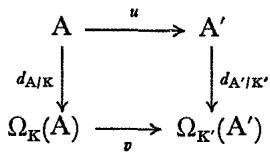
\includegraphics[keepaspectratio]{images/part004_9ff9737d.jpg}}

\(d_{\mathbf{A}^{\prime} / \mathbf{K}^{\prime}}\circ u\) is a K-derivation of A with values in the A-module \(\Omega_{\mathbf{K}^{\prime}}(\mathbf{A}^{\prime})\) ; the existence and uniqueness of \(v\) then follow from Proposition 18 of no. 11.

The mapping v of Proposition 19 will be denoted by \(\Omega(u)\) ; if there is a commutative diagram of commutative ring homomorphisms

\pandocbounded{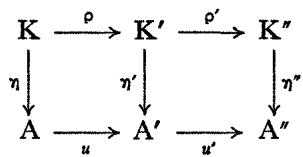
\includegraphics[keepaspectratio]{images/part004_26fbb1e8.jpg}}

it follows immediately from the uniqueness property of Proposition 19 that

\[
\Omega (u ^ {\prime} \circ u) = \Omega (u ^ {\prime}) \circ \Omega (u).
\]

Since \(\Omega_{\mathbf{K}'}(\mathbf{A}')\) is an \(\mathbf{A}'\) -module, from \(\Omega(u)\) we derive canonically an \(\mathbf{A}'\) -linear mapping

\[
\Omega_ {0} (u): \Omega_ {\mathbf {K}} (\mathrm{A}) \otimes_ {\mathrm{A}} \mathrm{A} ^ {\prime} \rightarrow \Omega_ {\mathbf {K} ^ {\prime}} (\mathrm{A} ^ {\prime})\tag{41}
\]

such that \(\Omega(u)\) is the composition of \(\Omega_0(u)\) and the canonical homomorphism \(i_{\mathbf{A}}: \Omega_{\mathbf{K}}(\mathbf{A}) \to \Omega_{\mathbf{K}}(\mathbf{A}) \otimes_{\mathbf{A}} \mathbf{A}'\) . For every \(\mathbf{A}'\) -module \(\mathbf{E}'\) , there is a commutative diagram

\pandocbounded{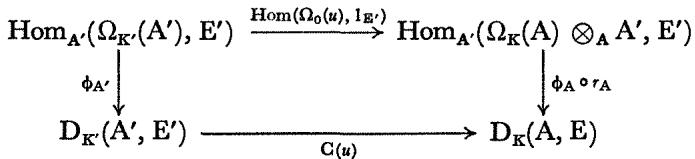
\includegraphics[keepaspectratio]{images/part004_95f64194.jpg}}

where \(\mathbf{C}(u)\) is the mapping \(D \mapsto D \circ u\) (no. 7, Proposition 9) and \(r_{A}\) is the canonical isomorphism

\[
\operatorname{Hom} \left(i _ {\mathrm{A}}, 1 _ {\mathrm{E} ^ {\prime}}\right): \operatorname{Hom} _ {\mathrm{A} ^ {\prime}} \left(\Omega_ {\mathrm{K}} (\mathrm{A}) \otimes_ {\mathrm{A}} \mathrm{A} ^ {\prime}, \mathrm{E} ^ {\prime}\right)\rightarrow \operatorname{Hom} _ {\mathrm{A}} \left(\Omega_ {\mathrm{K}} (\mathrm{A}), \mathrm{E} ^ {\prime}\right);
\]

this follows immediately from Proposition 19 and the definition of the isomorphisms \(\phi_{\mathbf{A}}\) and \(\phi_{\mathbf{A}^{\prime}}\) .

PROPOSITION 20. Suppose that \(\mathbf{A}' = \mathbf{A} \otimes_{\mathbb{K}} \mathbf{K}'\) , with \(\eta': \mathbf{K}' \to \mathbf{A}'\) and \(u: \mathbf{A} \to \mathbf{A}'\) the canonical homomorphisms. Then the \(\mathbf{A}'\) -linear mapping

\[
\Omega_ {0} (u): \Omega_ {\mathbf {K}} (\mathrm{A}) \otimes_ {\mathbf {A}} \mathrm{A} ^ {\prime} \rightarrow \Omega_ {\mathbf {K} ^ {\prime}} (\mathrm{A} ^ {\prime})
\]

is an isomorphism.

By virtue of the fact that in diagram (42) the vertical arrows are bijective, it reduces to proving that, for every A'-module E', the homomorphism C(u):D → D ∘ u in diagram (42) is bijective (II, § 2, no. 1, Theorem 1). Now Hom(u, 1\_E') : Hom\_K'(A ⊗\_K K', E') → Hom\_K(A, E') is an isomorphism (II, § 5, no. 1, Proposition 1) and C(u) is its restriction to D\_K'(A', E') and hence is injective; moreover, if f: A' → E' is a K'-linear mapping such that

\[
f \circ u: \mathrm{A} \rightarrow \mathrm{E} ^ {\prime}
\]

is a K-derivation, it follows immediately from the fact that \(f\) is \(\mathbf{K}'\) -linear and the fact that \(f((x \otimes 1)(y \otimes 1)) = (y \otimes 1)f(x \otimes 1) + (x \otimes 1)f(y \otimes 1)\) for \(x, y\) in A, that \(f\) is a \(\mathbf{K}'\) -derivation, the elements \(x \otimes 1\) for \(x \in A\) forming a generating system of the \(\mathbf{K}'\) -module \(A'\) ; this completes the proof that \(C(u)\) is bijective.

From now on we confine our attention to the case where \(\rho: \mathbf{K} \to \mathbf{K}'\) is the identity mapping of \(\mathbf{K}\) ; every K-algebra homomorphism \(u: \mathbf{A} \to \mathbf{B}\) is therefore mapped to a B-linear mapping

\[
\Omega_ {0} (u): \Omega_ {\mathbf {K}} (\mathrm{A}) \otimes_ {\mathbf {K}} \mathrm{B} \rightarrow \Omega_ {\mathbf {K}} (\mathrm{B}).\tag{43}
\]

On the other hand, we can consider the B-module of A-differentials \(\Omega_{\mathbf{A}}(\mathbf{B})\) since B is an A-algebra by means of u; the canonical derivation \(d_{\mathrm{B/A}}: \mathbf{B} \to \Omega_{\mathbf{A}}(\mathbf{B})\) being a fortiori a K-derivation, it factorizes uniquely into

\[
\mathbf {B} \xrightarrow {d _ {\mathbf {B} / \mathbf {K}}} \Omega_ {\mathbf {K}} (\mathbf {B}) \xrightarrow {\Omega_ {u}} \Omega_ {\mathbf {A}} (\mathbf {B})
\]

where \(\Omega_{u}\) is a B-linear mapping (no. 11, Proposition 18). For every B-module E, there is a commutative diagram

\[
\begin{array}{c} \operatorname{Hom} _ {\mathbf {B}} (\Omega_ {\mathbf {A}} (\mathbf {B}), \mathrm{E}) \xrightarrow {\operatorname{Hom} (\Omega_ {u} , 1 _ {\mathbf {E}})} \operatorname{Hom} _ {\mathbf {B}} (\Omega_ {\mathbf {K}} (\mathbf {B}), \mathrm{E}) \\ \phi_ {\mathbf {A}, \mathbf {B}} \Biggl \downarrow \\ \mathrm{D} _ {\mathbf {A}} (\mathrm{B}, \mathrm{E}) \xrightarrow [ j _ {u} ]{} \mathrm{D} _ {\mathbf {K}} (\mathrm{B}, \mathrm{E}) \end{array}\tag{44}
\]

where \(j_{u}\) is the canonical injection (no. 7); this follows immediately from Proposition 18 of no. 11.

PROPOSITION 21. The sequence of B-linear mappings

\[
\Omega_ {\mathbf {K}} (\mathrm{A}) \otimes_ {\mathbf {A}} \mathrm{B} \xrightarrow {\Omega_ {0} (u)} \Omega_ {\mathbf {K}} (\mathrm{B}) \xrightarrow {\Omega_ {u}} \Omega_ {\mathbf {A}} (\mathrm{B}) \to 0\tag{45}
\]

is exact.

It reduces to verifying that, for every B-module E, the sequence

\[
\begin{array}{c} 0 \to \operatorname{Hom} _ {\mathrm{B}} (\Omega_ {\mathrm{A}} (\mathrm{B}), \mathrm{E}) \xrightarrow {\operatorname{Hom} (\Omega_ {\mathrm{u}} , 1 _ {\mathrm{E}})} \operatorname{Hom} _ {\mathrm{B}} (\Omega_ {\mathrm{K}} (\mathrm{B}), \mathrm{E}) \\ \xrightarrow {\operatorname{Hom} (\Omega_ {0} (u) , 1 _ {\mathrm{E}})} \operatorname{Hom} _ {\mathrm{B}} (\Omega_ {\mathrm{K}} (\mathrm{A}) \otimes_ {\mathrm{A}} \mathrm{B}, \mathrm{E}) \end{array}
\]

is exact (II, §2, no. 1, Theorem 1); but by virtue of the fact that in the commutative diagrams (42) and (44) the vertical arrows are isomorphisms, it suffices to show that the sequence

\[
0 \longrightarrow \mathrm{D} _ {\mathrm{A}} (\mathrm{B}, \mathrm{E}) \xrightarrow {j _ {u}} \mathrm{D} _ {\mathrm{K}} (\mathrm{B}, \mathrm{E}) \xrightarrow {\mathrm{C} (u)} \mathrm{D} _ {\mathrm{K}} (\mathrm{A}, \mathrm{E})
\]

is exact, which is just Proposition 11 of no. 7.

We consider now the case where the K-algebra homomorphism \(u: \mathbf{A} \to \mathbf{B}\) is surjective; if \(\mathfrak{J}\) is its kernel, \(\mathbf{B}\) is then isomorphic to \(\mathbf{A} / \mathfrak{J}\) . We consider the restriction \(d| \mathfrak{J}: \mathfrak{J} \to \Omega_{\mathbf{K}}(\mathbf{A})\) of the canonical derivation \(d = d_{\mathbf{A} / \mathbf{K}}\) and the composite A-linear mapping

\[
d ^ {\prime}: \mathfrak {J} \xrightarrow {d | \mathfrak {J}} \Omega_ {\mathrm{K}} (\mathrm{A}) \xrightarrow {i _ {\mathrm{A}}} \Omega_ {\mathrm{K}} (\mathrm{A}) \otimes_ {\mathrm{A}} \mathrm{B}.
\]

Then \(d^{\prime}(\mathfrak{J}^{2}) = 0\) , since, for \(x, y\) in \(\mathfrak{J}\) ,

\[
d ^ {\prime} (x y) = d (x y) \otimes 1 = (x. d y + y. d x) \otimes 1 = d y \otimes u (x) + d x \otimes u (y) = 0
\]

since \(u(x) = u(y) = 0\) . Hence we derive from \(d'\) , by passing to the quotient, an A-linear mapping

\[
\bar {d} \colon \mathfrak {J} / \mathfrak {J} ^ {2} \rightarrow \Omega_ {\mathrm{K}} (\mathrm{A}) \otimes_ {\mathrm{A}} \mathrm{B}
\]

and as \(\mathfrak{J}\) annihilates the A-module \(\mathfrak{J} / \mathfrak{J}^2\) , \(\bar{d}\) is a B-linear mapping.

PROPOSITION 22. Let \(\mathfrak{J}\) be an ideal of the commutative K-algebra A, B = A/ \(\mathfrak{J}\) and \(u:A\to B\) the canonical homomorphism. The sequence of B-linear mappings

\[
\mathfrak {J} / \mathfrak {J} ^ {2} \xrightarrow {\overline {{d}}} \Omega_ {\mathrm{K}} (\mathrm{A}) \otimes_ {\mathrm{A}} \mathrm{B} \xrightarrow {\Omega_ {0} (u)} \Omega_ {\mathrm{K}} (\mathrm{B}) \to 0\tag{46}
\]

is then exact.

Note that \(\Omega_{\mathbf{K}}(\mathbf{A}) \otimes_{\mathbf{A}} \mathbf{B}\) is identified with \(\Omega_{\mathbf{K}}(\mathbf{A}) / \mathfrak{J} \Omega_{\mathbf{K}}(\mathbf{A})\) and that the image of \(\bar{d}\) is the image of \(d(\mathfrak{J})\) in this quotient module; the quotient of \(\Omega_{\mathbf{K}}(\mathbf{A}) \otimes_{\mathbf{A}} \mathbf{B}\) by \(\operatorname{Im}(\bar{d})\) is therefore identified with the quotient \(\Omega_{\mathbf{K}}(\mathbf{A}) / \mathbf{N}\) , where \(\mathbf{N}\) is the sub-A-module generated by \(\mathfrak{J} \Omega_{\mathbf{K}}(\mathbf{A})\) and \(d(\mathfrak{J})\) . Moreover, the composite mapping

\[
\mathrm{A} \xrightarrow {d _ {\mathrm{A} / \mathrm{K}}} \Omega_ {\mathrm{K}} (\mathrm{A}) \longrightarrow \Omega_ {\mathrm{K}} (\mathrm{A}) / \mathrm{N}
\]

is a K-derivation (no. 7, Proposition 9) and, since it is zero on \(\mathfrak{J}\) by definition of N, it defines, when passing to the quotient, a K-derivation \(D_0:B\to \Omega_{\mathbb{K}}(A) / N\) .

Taking account of the uniqueness of the solution of a universal mapping problem, it reduces to proving that, for every B-module E and every K-derivation D: B → E, there exists a unique B-linear mapping g: \(\Omega_{\mathrm{K}}(\mathrm{A})/\mathrm{N} \rightarrow \mathrm{E}\) such that \(D = g \circ D_{0}\) . But, the composite mapping D ∘ u: A → E is a K-derivation (no. 7, Proposition 9) and hence there exists one and only one A-linear mapping f: \(\Omega_{\mathrm{K}}(\mathrm{A}) \rightarrow \mathrm{E}\) such that \(f \circ d_{A/K} = D \circ u\) . This relation shows already that f is zero on \(d(\mathfrak{J})\) ; as also \(\mathfrak{J} E = \{0\}\) since E is a B-module, f is zero on \(\mathfrak{J} \Omega_{\mathrm{K}}(\mathrm{A})\) ; hence f is zero on N and defines, when passing to the quotient, a B-linear mapping g: \(\Omega_{\mathrm{K}}(\mathrm{A})/\mathrm{N} \rightarrow \mathrm{E}\) such that \(g \circ D_{0} = D\) ; the uniqueness of g follows from the uniqueness of f.

It must not be thought that, even if \(u: \mathbf{A} \to \mathbf{B}\) is an injective homomorphism, \(\Omega_0(u): \Omega_{\mathbf{K}}(\mathbf{A}) \otimes_{\mathbf{A}} \mathbf{B} \to \Omega_{\mathbf{K}}(\mathbf{B})\) is injective (Exercise 5). However we have the following proposition:

PROPOSITION 23. Let A be an integral K-algebra, B its field of fractions and \(u: \mathbf{A} \to \mathbf{B}\) the canonical injection. Then \(\Omega_0(u): \Omega_{\mathbf{K}}(\mathbf{A}) \otimes_{\mathbf{A}} \mathbf{B} \to \Omega_{\mathbf{K}}(\mathbf{B})\) is an isomorphism.

Using the fact that in diagram (42) the vertical arrows are bijective, it reduces to proving that, for every vector space E over B, the mapping \(\mathrm{C}(u):\mathrm{D}_{\mathrm{K}}(\mathrm{B},\mathrm{E})\to\mathrm{D}_{\mathrm{K}}(\mathrm{A},\mathrm{E})\) is bijective. But this follows from the fact that every K-derivation of A into E can be extended uniquely to a K-derivation of B into E (no. 5, Proposition 5).

\section{COGEBRAS, PRODUCTS OF MULTILINEAR FORMS, INNER PRODUCTS AND DUALITY}

In this paragraph, A is a commutative ring with the trivial graduation. For a graded A-module M of type N, \(M^{*gr}\) will denote the graded A-module of type N, whose homogeneous elements of degrees n are the A-linear forms which are zero on \(M_{k}\) for all \(k \neq n\) .

\subsection{COGEBRAS}

DEFINITION 1. A cogebra over A (or A-cogebra, or simply cogebra if no confusion can arise) is a set E with a structure defined by giving the following:

\begin{enumerate}
\def\labelenumi{(\arabic{enumi})}
\item
  an A-module structure on E;
\item
  an A-linear mapping \(c: \mathbf{E} \to \mathbf{E} \otimes_{\mathbf{A}} \mathbf{E}\) called the coproduct of \(\mathbf{E}\) .
\end{enumerate}

DEFINITION 2. Given two cogebras E, E', whose coproducts are denoted respectively by c and c', a morphism of E into E' is an A-linear mapping u; E → E' such that

\[
(u \otimes u) \circ c = c ^ {\prime} \circ u\tag{1}
\]

in other words, it renders commutative the diagram of A-linear mappings

\pandocbounded{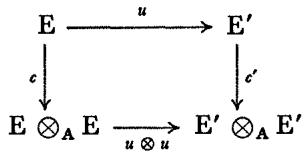
\includegraphics[keepaspectratio]{images/part004_6ed4336b.jpg}}

It is immediately verified that the identity mapping is a morphism, that the composition of two morphisms is a morphism and that every bijective morphism is an isomorphism.

Examples. (1) The canonical isomorphism \(\mathbf{A} \to \mathbf{A} \otimes_{\mathbf{A}} \mathbf{A}\) (II, § 3, no. 5) defines an A-cogebra structure on \(\mathbf{A}\) .

\begin{enumerate}
\def\labelenumi{(\arabic{enumi})}
\setcounter{enumi}{1}
\item
  Let E be a cogebra, c its coproduct and \(\sigma\) the canonical automorphism of the A-module \(E \otimes_{A} E\) such that \(\sigma(x \otimes y) = y \otimes x\) for \(x \in E\) , \(y \in E\) ; the A-linear mapping \(\sigma \circ c\) defines a new cogebra structure on E. With this structure E is called the opposite cogebra to the given cogebra E.
\item
  Let B be an A-algebra and let \(m:B \otimes_{A} B \to B\) be the A-linear mapping defining multiplication on B ( \(\S 1\) , no. 3). The transpose \(^{t}m\) is then an A-linear mapping of the dual \(B^{*}\) of the A-module B into the dual \((\mathbf{B} \otimes_{\mathbf{A}} \mathbf{B})^{*}\) of the A-module \(B \otimes_{A} B\) . If also B is a finitely generated projective A-module, the canonical mapping \(\mu:B^{*} \otimes_{A} B^{*} \to (\mathbf{B} \otimes_{\mathbf{A}} \mathbf{B})^{*}\) is an A-module isomorphism (II, \(\S 4\) , no. 4); the mapping \(c = \mu^{-1} \circ ^{t}m\) is then a coproduct defining a cogebra structure on the dual \(B^{*}\) of the A-module B.
\item
  Let X be a set, \(\mathbf{A}^{(\mathbf{X})}\) the A-module of formal linear combinations of elements of X with coefficients in A (II, §1, no. 11) and \((e_{x})_{x\in\mathbf{X}}\) the canonical basis of \(\mathbf{A}^{(\mathbf{X})}\) . An A-linear mapping \(c:A^{(\mathbf{X})}\to\mathbf{A}^{(\mathbf{X})}\otimes_{\mathbf{A}}\mathbf{A}^{(\mathbf{X})}\) is defined by the condition \(c(e_{x})=e_{x}\otimes e_{x}\) and a canonical cogebra structure is thus obtained on \(\mathbf{A}^{(\mathbf{X})}\) .
\item
  Let \(\mathbf{M}\) be an A-module and \(\mathsf{T}(\mathbf{M})\) the tensor algebra of \(\mathbf{M}\) ( \(\S 5\) , no. 1); by II, \(\S 3\) , no. 9 there exists one and only one A-linear mapping \(c\) of the A-module \(\mathsf{T}(\mathbf{M})\) into the A-module \(\mathsf{T}(\mathbf{M}) \otimes_{\mathbf{A}} \mathsf{T}(\mathbf{M})\) such that, for all \(n \geqslant 0\) ,
\end{enumerate}

\[
c (x _ {1} x _ {2} \dots x _ {n}) = \sum_ {0 \leqslant p \leqslant n} (x _ {1} x _ {2} \dots x _ {p}) \otimes (x _ {p + 1} \dots x _ {n})\tag{3}
\]

for all \(x_{i} \in \mathbf{M}\) ( \(x_{1}x_{2}\ldots x_{n}\) denotes the product in the algebra \(\mathsf{T}(\mathbf{M})\) ). Thus \(\mathsf{T}(\mathbf{M})\) is given a cogebra structure.

\begin{enumerate}
\def\labelenumi{(\arabic{enumi})}
\setcounter{enumi}{5}
\tightlist
\item
  Let M be an A-module and S(M) the symmetric algebra of M (§ 6, no. 1); the diagonal mapping \(\Delta: x \mapsto (x, x)\) of M into M × M is an A-linear mapping to which there therefore corresponds a homomorphism S(Δ) of the A-algebra S(M) into the A-algebra S(M × M) (§ 6, no. 2, Proposition 3). On the other hand, in § 6, no. 6 we defined a canonical graded algebra isomorphism \(h \colon \mathbb{S}(\mathbf{M} \times \mathbf{M}) \to \mathbb{S}(\mathbf{M}) \otimes_{\mathbf{A}} \mathbb{S}(\mathbf{M})\) ; by composition we therefore obtain an A-algebra homomorphism
\end{enumerate}

\[
c = h \circ \mathbf {S} (\Delta): \mathbf {S} (\mathbf {M}) \rightarrow \mathbf {S} (\mathbf {M}) \otimes_ {\mathbf {A}} \mathbf {S} (\mathbf {M}),
\]

thus defining on \(\mathbf{S}(\mathbf{M})\) a cogebra structure. For all \(x\in \mathbf{M}\) , by definition \(\mathbf{S}(\Delta)(x) = (x,x)\) and the definition of \(h\) given in § 6, no. 6 shows that

\[
h ((x, x)) = x \otimes 1 + 1 \otimes x.
\]

It follows that \(c\) is the unique algebra homomorphism such that, for all \(x \in \mathbf{M}\) ,

\[
c (x) = x \otimes 1 + 1 \otimes x.\tag{4}
\]

As \(c\) is an algebra homomorphism, it follows that, for every sequence \((x_{i})_{1\leqslant i\leqslant n}\) of \(n\) elements of \(\mathbf{M}\) ,

\[
\begin{array}{r l} c (x _ {1} x _ {2} \dots x _ {n}) & = \prod_ {i = 1} ^ {n} (x _ {i} \otimes 1 + 1 \otimes x _ {i}) \\ & = \sum (x _ {i _ {1}} \dots x _ {i _ {p}}) \otimes (x _ {j _ {1}} \dots x _ {j _ {n - p}}) \end{array}\tag{5}
\]

the summation on the right hand side of (5) being taken over all ordered pairs of strictly increasing sequences (in some cases empty)

\[
i _ {1} <   i _ {2} <   \dots <   i _ {p}, \quad j _ {1} <   j _ {2} <   \dots <   j _ {n - p}
\]

of elements of \([1, n]\) , whose sets of elements are complementary. The element \(c(x_1 x_2 \ldots x_n)\) is an element of total degree \(n\) in \(\mathbb{S}(\mathbf{M}) \otimes_{\mathbf{A}} \mathbb{S}(\mathbf{M})\) and its component of bidegree \((p, n - p)\) is

\[
\sum_ {\sigma} \left(x _ {\sigma (1)} \dots x _ {\sigma (p)}\right) \otimes \left(x _ {\sigma (p + 1)} \dots x _ {\sigma (n)}\right)\tag{6}
\]

where the summation is taken over all permutations \(\sigma\in\mathbb{S}_{n}\) which are increasing in each of the intervals \([1,p]\) and \([p+1,n]\) .

\begin{enumerate}
\def\labelenumi{(\arabic{enumi})}
\setcounter{enumi}{6}
\tightlist
\item
  Let \(\mathbf{M}\) be an A-module and proceed with the exterior algebra \(\bigwedge (\mathbf{M})\) as with \(\mathbb{S}(\mathbf{M})\) in Example 6; the diagonal mapping \(\Delta : \mathbf{M} \to \mathbf{M} \times \mathbf{M}\) this time defines a homomorphism \(\bigwedge (\Delta)\) of the A-algebra \(\bigwedge (\mathbf{M})\) into the A-algebra \(\bigwedge (\mathbf{M} \times \mathbf{M})\) (§ 7, no. 2, Proposition 2); on the other hand there is a canonical graded algebra isomorphism
\end{enumerate}

\[
h: \bigwedge (\mathbf {M} \times \mathbf {M}) \rightarrow \bigwedge (\mathbf {M}) ^ {\mathrm{g}} \otimes_ {\mathbf {A}} \bigwedge (\mathbf {M})
\]

(§ 7, no. 7, Proposition 10), whence by composition there is an algebra homomorphism \(c = h \circ \bigwedge(\Delta): \bigwedge(M) \to \bigwedge(M)^{\mathfrak{g}} \otimes_{A} \bigwedge(M)\) , which can be considered as an A-module homomorphism \(\bigwedge(M) \to \bigwedge(M) \otimes_{A} \bigwedge(M)\) and which therefore defines on \(\bigwedge(M)\) a cogebra structure. It can be proved as in Example 6 that \(c\) is the unique algebra homomorphism such that, for all \(x \in M\) ,

\[
c (x) = x \otimes 1 + 1 \otimes x,\tag{7}
\]

whence, for every sequence \((x_{i})_{1\leqslant i\leqslant n}\) of elements of \(\mathbf{M}\) ,

\[
c \left(x _ {1} \wedge x _ {2} \wedge \dots \wedge x _ {n}\right) = \left(x _ {1} \otimes 1 + 1 \otimes x _ {1}\right) \wedge \dots \wedge \left(x _ {n} \otimes 1 + 1 \otimes x _ {n}\right)
\]

where the product on the right hand side is taken in the algebra

\[
\Lambda (\mathbf {M}) ^ {\mathfrak {g}} \otimes_ {\mathbf {A}} \Lambda (\mathbf {M});
\]

to calculate this product, consider, for every ordered pair of strictly increasing sequences \(i_1 < i_2 < \cdots < i_p\) , \(j_1 < j_2 < \cdots < j_{n-p}\) of elements of \([1, n]\) , whose sets of elements are complementary, the product \(y_1y_2\ldots y_n\) , where \(y_{i_h} = x_{i_h} \otimes 1 (1 \leqslant h \leqslant p)\) and \(y_{j_k} = 1 \otimes x_{j_k} (1 \leqslant k \leqslant n - p)\) and the sum is taken over all these products. As the graded algebra \(\bigwedge (\mathbf{M})^{\mathfrak{g}} \otimes_{\mathbf{A}} \bigwedge (\mathbf{M})\) is anticommutative and the elements \(x_i \otimes 1\) and \(1 \otimes x_i\) are of total degree 1, by §4, no. 6, Lemma 3 and Lemma 1,

\[
\begin{array}{r l} c (x _ {1} \wedge x _ {2} \wedge \dots \wedge x _ {n}) & = \sum (- 1) ^ {\nu} (x _ {i _ {1}} \wedge \dots \wedge x _ {i _ {p}}) \otimes (x _ {j _ {1}} \wedge \dots \wedge x _ {j _ {n - p}}) \end{array} \tag {8}
\]

v being the number of ordered pairs \((h, k)\) such that \(j_{k} < i_{h}\) and the summation being taken over the same set as in (5). The element \(c(x_{1} \wedge \cdots \wedge x_{n})\) is of total degree n in \(\bigwedge(\mathbf{M})^{\mathbf{g}} \otimes_{\mathbf{A}} \bigwedge(\mathbf{M})\) and its homogeneous component of bi-degree \((p, n - p)\) is equal to

\[
\sum_ {\sigma} \varepsilon_ {\sigma} (x _ {\sigma (1)} \wedge \dots \wedge x _ {\sigma (p)}) \otimes (x _ {\sigma (p + 1)} \wedge \dots \wedge x _ {\sigma (n)})\tag{9}
\]

the summation being taken over permutations \(\sigma\in\mathfrak{S}_{n}\) which are increasing in each of the intervals \([1,p]\) and \([p+1,n]\) .

When in future we speak of \(\mathbf{A}^{(\mathbf{X})}\) , \(\mathsf{T}(\mathbf{M})\) , \(\mathsf{S}(\mathbf{M})\) or \(\bigwedge (\mathbf{M})\) as cogebras, we shall mean, unless otherwise mentioned, with the cogebra structures defined in Examples 4, 5, 6 and 7 respectively.

\begin{enumerate}
\def\labelenumi{(\arabic{enumi})}
\setcounter{enumi}{7}
\tightlist
\item
  Let E, F be two A-cogebras and c, \(c'\) their respective coproducts. Let \(\tau:(\mathbf{E} \otimes_{\mathbf{A}} \mathbf{E}) \otimes_{\mathbf{A}} (\mathbf{F} \otimes_{\mathbf{A}} \mathbf{F}) \to (\mathbf{E} \otimes_{\mathbf{A}} \mathbf{F}) \otimes_{\mathbf{A}} (\mathbf{E} \otimes_{\mathbf{A}} \mathbf{F})\) denote the associativity isomorphism such that \(\tau((x \otimes x') \otimes (y \otimes y')) = (x \otimes y) \otimes (x' \otimes y')\) for \(x, x'\) in E and \(y, y'\) in F. Then the composite linear mapping
\end{enumerate}

\[
\mathrm{E} \otimes_ {\mathrm{A}} \mathrm{F} \xrightarrow {c \otimes c ^ {\prime}} (\mathrm{E} \otimes_ {\mathrm{A}} \mathrm{E}) \otimes_ {\mathrm{A}} (\mathrm{F} \otimes_ {\mathrm{A}} \mathrm{F}) \xrightarrow {\tau} (\mathrm{E} \otimes_ {\mathrm{A}} \mathrm{F}) \otimes_ {\mathrm{A}} (\mathrm{E} \otimes_ {\mathrm{A}} \mathrm{F})
\]

defines a cogebra structure on the A-module E \(\otimes_{\mathbf{A}}\mathbf{F}\) , called the tensor product of the cogebras E and F.

Let E be a cogebra and \(\Delta\) a commutative monoid. A graduation \((\mathrm{E}_{\lambda})_{\lambda\in\Delta}\) on the A-module E is said to be compatible with the coproduct c of E if c is a graded homomorphism of degree 0 of the graded A-module E into the graded A-module (of type \(\Delta\) ) \(E\otimes_{A}E\) , in other words (II, §11, no. 5) if

\[
\mathrm{c} (\mathrm{E} _ {\lambda}) \subset \sum_ {\mu + \nu = \lambda} \mathrm{E} _ {\mu} \otimes_ {\mathbf {A}} \mathrm{E} _ {\nu}.\tag{10}
\]

In what follows, we shall most often limit our attention to graduations of type N compatible with the coproduct; a cogebra with such a graduation will also be called a graded cogebra. If F is another graded cogebra, a graded cogebra morphism \(\phi:E\to F\) is by definition a cogebra morphism (Definition 2) which is also a graded homomorphism of degree 0 of graded A-modules.

Examples. (9) It is immediate that the cogebras \(\mathsf{T}(\mathbf{M})\) , \(\mathsf{S}(\mathbf{M})\) and \(\bigwedge (\mathbf{M})\) defined above are graded cogebras.

\subsection{COASSOCIATIVITY, COCOMMUTATIVITY, COUNIT}

Let E be a cogebra, c its coproduct, N, N', N'' three A-modules and m a bilinear mapping of N × N' into N''. Let \(\tilde{m}:N \otimes_{A} N' \to N''\) denote the A-linear mapping corresponding to m. If \(u:E \to N\) , \(v:E \to N'\) are two A-linear mappings, we derive an A-linear mapping \(u \otimes v:E \otimes_{A} E \to N \otimes_{A} N'\) and a composite A-linear mapping of E into N'':

\[
m (u, v): \mathrm{E} \xrightarrow {c} \mathrm{E} \otimes_ {\mathrm{A}} \mathrm{E} \xrightarrow {u \otimes v} \mathrm{N} \otimes_ {\mathrm{A}} \mathrm{N} ^ {\prime} \xrightarrow {\tilde {m}} \mathrm{N} ^ {\prime \prime}.\tag{11}
\]

Clearly we have thus defined an A-bilinear mapping \((u, v) \mapsto m(u, v)\) of \(\operatorname{Hom}_{\mathbf{A}}(\mathbf{E}, \mathbf{N}) \times \operatorname{Hom}_{\mathbf{A}}(\mathbf{E}, \mathbf{N}')\) into \(\operatorname{Hom}_{\mathbf{A}}(\mathbf{E}, \mathbf{N}'')\) .

When E is a graded cogebra, N, N', N'' graded A-modules of the same type and \(\tilde{m}\) a graded homomorphism of degree k of N \(\otimes_{A}N'\) into N'', then, if u (resp. v) is a graded homomorphism of degree p (resp. q), \(m(u,v)\) is a graded homomorphism of degree \(p + q + k\) .

Examples. (1) Take E to be the graded cogebra T(M) (no. 1) and suppose that N, N', N'' have the trivial graduation. A graded homomorphism of degree -p of T(M) into N (resp. N', N'') then corresponds to a multilinear mapping of M\^{}p into N (resp. N', N''). Given a multilinear mapping u: M\^{}p → N and a multilinear mapping v: M\^{}q → N', the above method allows us to deduce a multilinear mapping m(u, v): M\^{}\{p+q\} → N'' called the product (relative to m) of u and v. Formulae (3) (no. 1) and (11) show that, for x\_1, . . ., x\_p+q in M,

\[
(m (u, v)) \left(x _ {1}, \dots , x _ {p + q}\right) = m \left(u \left(x _ {1}, \dots , x _ {p}\right), v \left(x _ {p + 1}, \dots , x _ {p + q}\right)\right).
\]

\begin{enumerate}
\def\labelenumi{(\arabic{enumi})}
\setcounter{enumi}{1}
\tightlist
\item
  Take E to be the graded cogebra S(M) (no. 1), preserving the same hypotheses on N, N', N''. A graded homomorphism of degree -p of S(M) into N then corresponds to a symmetric multilinear mapping of M \(^{p}\) into N (§ 6, no. 3). Then we derive from a symmetric multilinear mapping u: M \(^{p}\) → N and a symmetric multilinear mapping v: M \(^{q}\) → N' a symmetric multilinear mapping m(u, v): M \(^{p+q}\) → N'', also denoted (to avoid confusion) by \(u \cdot_{m} v\) (or even \(u \cdot v\)) and called the symmetric product (relative to m) of u and v. Formulae (6) (no. 1) and (11) show that, for x₁, \ldots, x \(_{p+q}\) in M,
\end{enumerate}

\[
(u \cdot_{m} v) (x _ {1}, \dots , x _ {p + q}) = \sum_ {\sigma} m (u (x _ {\sigma (1)}, \dots , x _ {\sigma (p)}), v (x _ {\sigma (p + 1)}, \dots , x _ {\sigma (p + q)}))
\]

the summation being taken over permutations \(\sigma\in\mathfrak{S}_{p+q}\) which are increasing on each of the intervals \([1,p]\) and \([p+1,p+q]\) .

\begin{enumerate}
\def\labelenumi{(\arabic{enumi})}
\setcounter{enumi}{2}
\tightlist
\item
  Take E to be the graded cogebra \(\bigwedge (\mathbf{M})\) (no. 1). Then we deduce similarly from an alternating multilinear mapping \(u: \mathbf{M}^p \to \mathbf{N}\) and an alternating multilinear mapping \(v: \mathbf{M}^q \to \mathbf{N}'\) an alternating multilinear mapping \(m(u, v): \mathbf{M}^{p + q} \to \mathbf{N}''\) , also denoted by \(u \wedge_m v\) or \(u \wedge v\) and called the alternating product (relative to \(m\) ) of \(u\) and \(v\) . Formulae (9) (no. 1) and (11) show in this case that, for \(x_1, \ldots, x_{p + q}\) in \(\mathbf{M}\) ,
\end{enumerate}

\[
(u \wedge_ {m} v) (x _ {1}, \dots , x _ {p + q}) = \sum_ {\sigma} \varepsilon_ {\sigma} m (u (x _ {\sigma (1)}, \dots , x _ {\sigma (p)}), v (x _ {\sigma (p + 1)}, \dots , x _ {\sigma (p + q)}))
\]

the summation again being taken over permutations \(\sigma \in \mathfrak{S}_{p + q}\) which are increasing on each of the intervals \([1, p]\) and \([p + 1, p + q]\) .

We return to the case where E is an arbitrary graded cogebra (of type N) and assume that the three modules N, N', N'' are all equal to the underlying A-module of a graded A-algebra B of type Z, the mapping m being multiplication in B, so that \(\tilde{m}:B\otimes_{A}B\to B\) is a graded A-linear mapping of degree 0. Thus a graded A-algebra structure is obtained on the graded A-module \(\operatorname{Homgr}_{A}(E,B)=C\) .

In particular, suppose that B = A (with the trivial graduation), so that \(\operatorname{Homgr}_{\mathbf{A}}(\mathbf{E}, \mathbf{A})\) is the graded dual \(E^{*gr}\) , which thus has a graded A-algebra structure.

Let F be another graded cogebra \(c'\) its coproduct and \(\phi:E\to F\) a graded cogebra morphism (no. 1); then the canonical graded morphism

\[
\tilde {\phi} = \operatorname{Hom} (\phi , 1 _ {B}): \operatorname{Homgr} _ {A} (F, B) \rightarrow \operatorname{Homgr} _ {A} (E, B)
\]

is a graded algebra homomorphism. For \(u, v\) in \(\operatorname{Homgr}_{\mathbf{A}}(\mathbf{F}, \mathbf{B})\) and \(x \in \mathbf{E}\) ,

\[
(\tilde {\phi} (u v)) (x) = (u v) (\phi (x)) = m ((u \otimes v) (c ^ {\prime} (\phi (x))))
\]

But by hypothesis \(c'(\phi(x)) = (\phi \otimes \phi)(c(x))\) , hence

\[
(u \otimes v) (c ^ {\prime} (\phi (x))) = (\tilde {\phi} (u) \otimes \tilde {\phi} (v)) (c (x))
\]

and therefore \(\tilde{\phi}(uv) = \tilde{\phi}(u)\tilde{\phi}(v)\) , which proves our assertion.

In particular, the graded transpose \({}^{t}\phi: \mathrm{F}^{*gr} \to \mathrm{E}^{*gr}\) is a graded algebra homomorphism.

Remark. Suppose that the \(E_{p}\) are finitely generated projective A-modules, so that the graded A-modules ( \(E \otimes_{A} E)^{*gr}\) and \(E^{*gr} \otimes_{A} E^{*gr}\) can be canonically identified (II, §4, no. 4, Corollary 1 to Proposition 4). If also the A-modules \(A \otimes_{A} A\) and A are then canonically identified (II, §3, no. 4), the linear mapping \(E^{*gr} \otimes_{A} E^{*gr} \to E^{*gr}\) which defines multiplication in \(E^{*gr}\) can be called the graded transpose of the coproduct c.

PROPOSITION 1. Let E be a cogebra over A. In order that, for every associative A-algebra B, the A-algebra \(\operatorname{Hom}_{\mathbf{A}}(\mathbf{E}, \mathbf{B})\) be associative, it is necessary and sufficient that the coproduct \(c: \mathbf{E} \to \mathbf{E} \otimes_{\mathbf{A}} \mathbf{E}\) be such that the diagram

\begin{enumerate}
\def\labelenumi{(\arabic{enumi})}
\setcounter{enumi}{11}
\tightlist
\item
\end{enumerate}

\pandocbounded{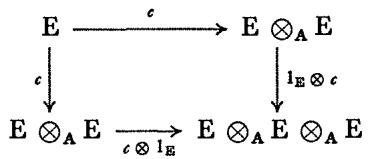
\includegraphics[keepaspectratio]{images/part004_a79ed2ff.jpg}}

be commutative.

Let B be an associative A-algebra and u, v, w three elements of \(\mathbf{C} = \operatorname{Hom}_{\mathbf{A}}(\mathbf{E}, \mathbf{B})\) . Let \(m_{3}\) denote the A-linear mapping \(B \otimes_{A} B \otimes_{A} B \to B\) which maps \(b \otimes b' \otimes b''\) to \(bb'b''\) . By definition of the product on the algebra C, \((uv)w\) is the composite mapping

\[
\mathrm{E} \xrightarrow {c} \mathrm{E} \otimes \mathrm{E} \xrightarrow {c \otimes 1 _ {\mathrm{E}}} \mathrm{E} \otimes \mathrm{E} \otimes \mathrm{E} \xrightarrow {u \otimes v \otimes w} \mathrm{B} \otimes \mathrm{B} \otimes \mathrm{B} \xrightarrow {m _ {3}} \mathrm{B}
\]

whilst \(u(vw)\) is the composite mapping

\[
\mathrm{E} \xrightarrow {c} \mathrm{E} \otimes \mathrm{E} \xrightarrow {1 _ {\mathrm{E}} \otimes c} \mathrm{E} \otimes \mathrm{E} \otimes \mathrm{E} \xrightarrow {u \otimes v \otimes w} \mathrm{B} \otimes \mathrm{B} \otimes \mathrm{B} \xrightarrow {m _ {3}} \mathrm{B}.
\]

It follows that if diagram (12) is commutative, the algebra \(\operatorname{Hom}_{\mathbf{A}}(\mathbf{E}, \mathbf{B})\) is associative for every associative A-algebra B. To establish the converse, it suffices to show that there exists an associative A-algebra B and three A-linear mappings \(u, v, w\) of E into B such that the mapping \(m_3 \circ (u \otimes v \otimes w)\) of \(\mathbf{E} \otimes \mathbf{E} \otimes \mathbf{E}\) into B is injective. Take B to be the A-algebra \(\mathsf{T}(\mathbf{E})\) and \(u, v, w\) the canonical mapping of E into \(\mathsf{T}(\mathbf{E})\) . The mapping \(m_3 \circ (u \otimes v \otimes w)\) is then the canonical mapping \(\mathbf{E} \otimes \mathbf{E} \otimes \mathbf{E} = \mathsf{T}^3(\mathbf{E}) \to \mathsf{T}(\mathbf{E})\) , which is injective.

When the cogebra E satisfies the condition of Proposition 1, it is said to be coassociative.

Examples. (4) It is immediately verified that the cogebra A (no. 1, Example (1)) the cogebra \(\mathbf{A}^{(\mathbf{X})}\) (no. 1, Example 4) and the cogebra \(\mathbf{T}(\mathbf{M})\) (no. 1, Example 5) are coassociative. If B is an associative A-algebra which is a finitely generated projective A-module, the cogebra \(\mathbf{B}^*\) (no. 1, Example 3) is coassociative: for the commutativity of diagram (12) then follows by transposition from that of the diagram which expresses the associativity of B ( \(\S\) 1, no. 3). Conversely, the same argument and the canonical identification of the A-module B with its bidual (II, § 2, no. 7, Corollary 4 to Proposition 13) show that if the cogebra \(\mathbf{B}^*\) is coassociative, the algebra \(\mathbf{B}\) is associative. Finally, the cogebras \(\mathsf{S}(\mathbf{M})\) and \(\bigwedge (\mathbf{M})\) (no. 1, Examples 6 and 7) are coassociative; this follows from the commutativity of the diagram

\[
\begin{array}{c} \mathrm{M} \xrightarrow {\Delta} \mathrm{M} \times \mathrm{M} \\ \Delta \Biggl \downarrow \\ \mathrm{M} \times \mathrm{M} \xrightarrow [ \Delta \times 1 _ {\mathrm{M}} ]{} \mathrm{M} \times \mathrm{M} \times \mathrm{M} \end{array}
\]

the functorial properties of \(\mathsf{S}(\mathbf{M})\) ( \(\S 6\) , no. 2) and \(\bigwedge (\mathbf{M})\) ( \(\S 7\) , no. 2), which give the corresponding commutative diagrams

\[
\left\{ \begin{array}{c} \mathsf {S} (\mathbf {M}) \xrightarrow {\mathsf {S} (\Delta)} \mathsf {S} (\mathbf {M} \times \mathbf {M}) \\ \mathsf {S} (\Delta) \Biggl \downarrow \qquad \qquad \qquad \qquad \qquad \qquad \qquad \qquad \qquad \qquad \qquad \qquad \qquad \qquad \qquad \qquad \qquad \qquad \qquad \qquad \qquad \qquad \qquad \qquad \qquad \qquad \qquad \qquad \qquad \qquad \qquad \qquad \qquad \qquad \mathsf {S} (1 _ {\mathbf {M}} \times \Delta) \\ \mathsf {S} (\mathbf {M} \times \mathbf {M}) \xrightarrow [ \mathsf {S} (\Delta \times 1 _ {\mathbf {M}}) ]{\mathsf {S} (\Delta \times 1 _ {\mathbf {M}})} \mathsf {S} (\mathbf {M} \times \mathbf {M} \times \mathbf {M}) \\ \bigwedge (\mathbf {M}) \xrightarrow {\bigwedge (\Delta)} \bigwedge (\mathbf {M} \times \mathbf {M}) \\ \bigwedge (\Delta) \Biggl \downarrow \qquad \qquad \qquad \qquad \qquad \qquad \qquad \qquad \qquad \qquad \qquad \qquad \qquad \bigwedge (1 _ {\mathbf {M}} \times \Delta) \\ \bigwedge (\mathbf {M} \times \mathbf {M}) \xrightarrow [ \bigwedge (\Delta \times 1 _ {\mathbf {M}}) ]{\bigwedge (\Delta \times 1 _ {\mathbf {M}})} \bigwedge (\mathbf {M} \times \mathbf {M} \times \mathbf {M}) \end{array} \right.\tag{14}
\]

and the existence and functoriality of canonical isomorphisms for symmetric and exterior algebras of a direct sum (§ 6, no. 6 and § 7, no. 7).

PROPOSITION 2. Let E be a cogebra over A. In order that, for every commutative A-algebra B, the A-algebra \(\operatorname{Hom}_{\mathbf{A}}(\mathbf{E}, \mathbf{B})\) be commutative, it is necessary and sufficient that the coproduct \(c: \mathbf{E} \to \mathbf{E} \otimes_{\mathbf{A}} \mathbf{E}\) be such that the diagram

\begin{enumerate}
\def\labelenumi{(\arabic{enumi})}
\setcounter{enumi}{14}
\tightlist
\item
\end{enumerate}

\pandocbounded{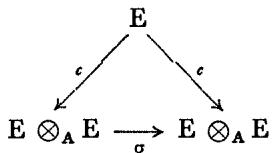
\includegraphics[keepaspectratio]{images/part004_07c99209.jpg}}

(where \(\sigma\) is the symmetry homomorphism such that \(\sigma(x \otimes y) = y \otimes x\) ) is commutative (in other words, it suffices that the cogebra E be identical with its opposite (no. 1, Example 2).

Let B be a commutative A-algebra and u, v two elements of C = Hom\_A(E, B).

By definition of the product in C, uv and vu are respectively equal to the composite mappings

\[
\mathrm{E} \xrightarrow {c} \mathrm{E} \otimes \mathrm{E} \xrightarrow {u \otimes v} \mathrm{B} \otimes \mathrm{B} \xrightarrow {m} \mathrm{B}
\]

and

\[
\mathrm{E} \xrightarrow {c} \mathrm{E} \otimes \mathrm{E} \xrightarrow {v \otimes u} \mathrm{B} \otimes \mathrm{B} \xrightarrow {m} \mathrm{B}.
\]

It follows that if diagram (15) is commutative the algebra \(\operatorname{Hom}_{\mathbf{A}}(\mathbf{E}, \mathbf{B})\) is commutative for every commutative A-algebra B. To establish the converse, it suffices to show that there exist a commutative A-algebra B and two A-linear mappings \(u, v\) of E into B such that \(m \circ (u \otimes v): \mathbf{E} \otimes \mathbf{E} \to \mathbf{B}\) is injective. Take B to be the algebra \(\mathsf{S}(\mathbf{E} \oplus \mathbf{E})\) and \(u\) (resp. \(v\) ) the composition of the canonical mapping \(\mathbf{E} \oplus \mathbf{E} \to \mathsf{S}(\mathbf{E} \oplus \mathbf{E})\) and the mapping \(x \mapsto (x, 0)\) (resp. \(x \mapsto (0, x)\) ) of E into \(\mathbf{E} \oplus \mathbf{E}\) . If \(h: \mathsf{S}(\mathbf{E}) \otimes \mathsf{S}(\mathbf{E}) \to \mathsf{S}(\mathbf{E} \otimes \mathbf{E})\) is the canonical isomorphism ( \(\S 6\) , no. 6, Proposition 9) and \(\lambda: \mathbf{E} \to \mathsf{S}(\mathbf{E})\) is the canonical mapping, then \(h^{-1} \circ m \circ (u \otimes v) = \lambda \otimes \lambda\) . Now \(\lambda \otimes \lambda\) is injective, for \(\lambda(\mathbf{E})\) is a direct factor of \(\mathsf{S}(\mathbf{E})\) (II, § 3, no. 7, Corollary 5 to Proposition 7).

When the cogebra E satisfies the condition of Proposition 2, it is said to be cocommutative.

Examples. (5) It is immediate that the cogebra A (no. 1, Example 1) and the cogebra \(\mathbf{A}^{(\mathbf{X})}\) (II, § 11, no. 1, Example 4) are cocommutative. It follows from formula (5) of no. 1 that the cogebra S(M) is cocommutative. Finally, for an A-algebra B such that the A-module B is projective and finitely generated to have the property that the cogebra \(\mathbf{B}^*\) (no. 1, Example 3) is cocommutative, it is necessary and sufficient that B be commutative; for (using the canonical identification of the A-module B with its bidual (II, § 2, no. 7)), this follows from the fact that the commutativity of diagram (14) is equivalent by transposition to that of the diagram which expressed the commutativity of B (§ 1, no. 3).

PROPOSITION 3. Let E be a cogebra over A. In order that, for every unital A-algebra B, the A-algebra \(\operatorname{Hom}_{\mathbf{A}}(\mathbf{E},\mathbf{B})\) be unital, it is necessary and sufficient that there exist a linear form \(\gamma\) on E rendering commutative the diagrams

\begin{enumerate}
\def\labelenumi{(\arabic{enumi})}
\setcounter{enumi}{15}
\tightlist
\item
\end{enumerate}

\pandocbounded{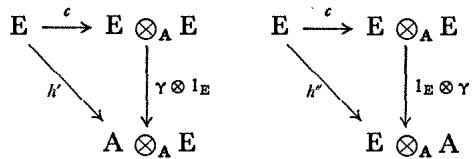
\includegraphics[keepaspectratio]{images/part004_cc0e83d1.jpg}}

where \(c: \mathbf{E} \to \mathbf{E} \otimes_{\mathbf{A}} \mathbf{E}\) is the coproduct and \(h'\) and \(h''\) the canonical isomorphisms (II, § 3, no. 4, Proposition 4). The unit of \(\operatorname{Hom}_{\mathbf{A}}(\mathbf{E}, \mathbf{B})\) is then the linear mapping \(x \mapsto \gamma(x)1\) (where 1 denotes the unit element of B).

Let \(\gamma\) be a linear form on E rendering diagram (16) commutative. Let B be a unital A-algebra with unit element 1, \(\eta: \mathbf{A} \to \mathbf{B}\) the canonical mapping and \(v = \eta \circ \gamma\) the element of the A-algebra \(\mathbf{C} = \operatorname{Hom}_{\mathbf{A}}(\mathbf{E}, \mathbf{B})\) . For every element \(u \in \mathbf{C}\) , \(uv\) is the composite mapping

\[
\mathrm{E} \xrightarrow {c} \mathrm{E} \otimes \mathrm{E} \xrightarrow {1 _ {\mathrm{E}} \otimes \gamma} \mathrm{E} \otimes \mathrm{A} \xrightarrow {u \otimes \eta} \mathrm{B} \otimes \mathrm{B} \xrightarrow {m} \mathrm{B}.\tag{17}
\]

Then \(uv = m \circ (u \otimes \eta) \circ h'' = u\) . It is similarly proved that \(vu = u\) and hence \(v\) is unit element of C. Conversely, let the A-module A ⊕ E be given a unital algebra structure such that \((a, x)(a', x') = (aa', ax' + a'x)\) for \(a, a'\) in A and \(x, x'\) in E. Let B denote the A-algebra thus defined and let C be the A-algebra Hom \(_A(E, B)\) . Suppose that C is unital and let \(e: x \mapsto (\gamma(x), \lambda(x))\) be its unit element (where \(\gamma(x) \in A\) and \(\lambda(x) \in E\) ). On the other hand let \(f\) be the element \(x \mapsto (0, x)\) of C. An immediate calculation shows that \(fe\) is the element

\[
x \mapsto (0, (h ^ {\prime \prime}) ^ {- 1} ((1 _ {E} \otimes \gamma) (c (x))))
\]

of C. The condition \(fe = f\) implies the commutativity of the second diagram of (16) and it is similarly seen that the condition \(ef = f\) implies the commutativity of the first diagram of (16).

A linear form \(\gamma\) on E rendering diagrams (16) commutative is called a counit of the cogebra E. A cogebra admits at most one counit: for it is the unit element of the algebra \(\operatorname{Hom}_{\mathbf{A}}(\mathbf{E}, \mathbf{A})\) . A cogebra with a counit is called counital.

Examples. (6) The identity mapping is the counit of the cogebra A; on the cogebra \(\mathbf{A}^{(\mathbf{X})}\) (no. 1, Example 4) the linear form \(\gamma\) such that \(\gamma(e_x) = 1\) for all \(x \in \mathbf{X}\) is the counit. On the cogebra \(\mathbf{T}(\mathbf{M})\) (resp. \(\mathbf{S}(\mathbf{M}), \bigwedge(\mathbf{M})\) ) the linear form \(\gamma\) such that \(\gamma(1) = 1\) and \(\gamma(z) = 0\) for \(z\) in the \(\mathbf{T}^n(\mathbf{M})\) (resp. \(\mathbf{S}^n(\mathbf{M}), \bigwedge^n(\mathbf{M})\) ) for \(n \geqslant 1\) is the counit. Finally, let B be an A-algebra which is a finitely generated projective A-module and has a unit element \(e\) ; then on the cogebra \(\mathbf{B}^*\) (no. 1, Example 3) the linear form \(\gamma: x^* \mapsto \langle e, x^* \rangle\) is the counit, for this form is just the transpose of the A-linear mapping \(\eta_e: \xi \mapsto \xi e\) of A into B and by transposition the commutativity of diagrams (16) follows from that of the diagrams which express (using \(\eta_e\) ) the fact that \(e\) is unit element of B ( \(\S 1\) , no. 3); the same argument moreover shows that conversely, if the cogebra \(\mathbf{B}^*\) admits a counit \(\gamma\) , the transpose of \(\gamma\) defines a unit element \(e = {}^t\gamma(1)\) of B.

PROPOSITION 4. Let E be a cogebra admitting a counit \(\gamma\) and suppose that there exists in E an element \(e\) such that \(\gamma(e) = 1\) ; then E is the direct sum of the sub-A-modules Ae and \(\mathrm{E}_{\gamma} = \mathrm{Ker}(\gamma)\) and

\[
c (e) \equiv e \otimes e (\mathrm{mod.} \mathrm{E} _ {\gamma} \otimes \mathrm{E} _ {\gamma})\tag{18}
\]

\[
\left\{c (x) \equiv x \otimes e + e \otimes x (\mathrm{mod.} \mathrm{E} _ {\gamma} \otimes \mathrm{E} _ {\gamma}) \quad \text { for all } x \in \mathrm{E} _ {\gamma}. \right.
\]

The first assertion is immediate, for \(\gamma(x - \gamma(x)e) = 0\) and the relation \(\gamma(\alpha e) = 0\) implies \(\alpha = 0\) . Let \(c(e) = \sum_{i} s_i \otimes t_i\) , so that

\[
e = \sum_ {i} \gamma (s _ {i}) t _ {i} = \sum_ {i} \gamma (t _ {i}) s _ {i}
\]

by (16) and \(1 = \gamma(e) = \sum_{i} \gamma(s_i) \gamma(t_i)\) . Therefore

\[
\begin{array}{r l} \sum_ {i} (s _ {i} - \gamma (s _ {i}) e) \otimes (t _ {i} - \gamma (t _ {i}) e) & = \sum_ {i} s _ {i} \otimes t _ {i} - \sum_ {i} e \otimes \gamma (s _ {i}) t _ {i} \\ & - \sum_ {i} \gamma (t _ {i}) s _ {i} \otimes e \\ & + \sum_ {i} \gamma (s _ {i}) e \otimes \gamma (t _ {i}) e \end{array}
\]

which, by the above relation, is just \(c(e) - e \otimes e\) ; this therefore proves the first relation of (18). On the other hand the decomposition of E \(\otimes\) E as a direct sum

\[
\mathbf {A} (e \otimes e) \oplus ((\mathbf {A} e) \otimes \mathbf {E} _ {\gamma}) \oplus (\mathbf {E} _ {\gamma} \otimes (\mathbf {A} e)) \oplus (\mathbf {E} _ {\gamma} \otimes \mathbf {E} _ {\gamma})
\]

allows us to write, for \(x \in \mathbf{E}_{\gamma}\) , \(c(x) = \lambda(e \otimes e) + (e \otimes y) + (z \otimes e) + u\) where \(u = \sum_{j} v_{j} \otimes w_{j}, y, z\) and the \(v_{j}\) and \(w_{j}\) belong to \(\mathbf{E}_{\gamma}\) . The definition of the counit \(\gamma\) then gives \(x = \lambda e + y = \lambda e + z\) and, as \(\gamma(x) = 0\) , necessarily \(\lambda = 0, x = y = z\) , whence the second relation of (18).

Remark. Let C be a counital coassociative A-coalgebra, B a unital associative A-algebra and M a left B-module. The A-bilinear mapping \((b, m) \mapsto bm\) of \(B \times M\) into M defines an A-bilinear mapping

\[
\operatorname{Hom} _ {\mathbf {A}} (\mathrm{C}, \mathrm{B}) \times \operatorname{Hom} _ {\mathbf {A}} (\mathrm{C}, \mathrm{M}) \rightarrow \operatorname{Hom} _ {\mathbf {A}} (\mathrm{C}, \mathrm{M})
\]

by the general procedure described at the beginning of this no. It is immediately verified that this mapping defines on \(\operatorname{Hom}_{\mathbf{A}}(\mathbf{C}, \mathbf{M})\) a left module structure over the ring \(\operatorname{Hom}_{\mathbf{A}}(\mathbf{C}, \mathbf{B})\) .

\subsection{PROPERTIES OF GRADED COGEBRAS OF TYPE N}

PROPOSITION 5. (i) Let E be a graded cogebra admitting a counit \(\gamma\) ; then \(\gamma\) is a homogeneous linear form of degree 0.

\begin{enumerate}
\def\labelenumi{(\roman{enumi})}
\setcounter{enumi}{1}
\tightlist
\item
  Suppose further that there exists an element \(e \in \mathbf{E}\) such that \(\mathbf{E}_0 = \mathbf{A}e\) and \(\gamma(e) = 1\) . Then the kernel \(\mathbf{E}_{\gamma}\) of \(\gamma\) is equal to \(\mathbf{E}_{+} = \sum_{n \geqslant 1} \mathbf{E}_n, c(e) = e \otimes e\) and
\end{enumerate}

\[
c (x) \equiv x \otimes e + e \otimes x (\mathrm{mod.} \mathrm{E} _ {+} \otimes \mathrm{E} _ {+})\tag{19}
\]

for all \(x \in \mathbf{E}_{+}\) .

\begin{enumerate}
\def\labelenumi{(\roman{enumi})}
\tightlist
\item
  It suffices to verify that \(\gamma(x) = 0\) for \(x \in \mathbf{E}_n\) , for all \(n \geqslant 1\) . Since \(c\) is a graded homomorphism of degree 0,
\end{enumerate}

\[
c (x) = \sum_ {0 \leqslant j \leqslant n} \left(\sum_ {i} y _ {i j} \otimes z _ {i, n - j}\right)\tag{20}
\]

with, for all \(j\) such that \(0 \leqslant j \leqslant n\) , \(y_{ij}\) and \(z_{ij}\) in \(\mathbf{E}_j\) ; applying (16) (no. 2) we obtain

\[
x = \sum_ {0 \leqslant j \leqslant n} \left(\sum_ {i} \gamma (y _ {i j}) z _ {i, n - j}\right) = \sum_ {0 \leqslant j \leqslant n} \left(\sum_ {i} \gamma (z _ {i, n - j}) y _ {i j}\right),
\]

whence, equating the components of degree 0 and degree n on the two sides

\[
x = \sum_ {i} \gamma (y _ {i 0}) z _ {i n} = \sum_ {i} \gamma (z _ {i 0}) y _ {i n}
\]

\[
0 = \sum_ {i} \gamma (y _ {i n}) z _ {i 0} = \sum_ {i} \gamma (z _ {i n}) y _ {i 0}
\]

and therefore \(\gamma(x) = \sum_{i} \gamma(y_{in})\gamma(z_{i0}) = \gamma(0) = 0\) .

\begin{enumerate}
\def\labelenumi{(\roman{enumi})}
\setcounter{enumi}{1}
\tightlist
\item
  Since \(\operatorname{Ker}(\gamma)\) and \(\mathbf{E}_{+}\) are both supplementary sub-A-modules of \(Ae = E_0\) and \(\mathbf{E}_{+} \subset \operatorname{Ker}(\gamma)\) by (i), \(\mathbf{E}_{+} = \operatorname{Ker}(\gamma)\) (II, § 1, no. 8, Remark 1); the other assertions follow from Proposition 4 of no. 2.
\end{enumerate}

PROPOSITION 6. Let E be a graded cogebra over A. In order that, for every commutative A-algebra B, with the trivial graduation, the graded A-algebra of type Z Homgr \(_{A}\) (E, B) (no. 2) be anticommutative (§ 4, no. 9, Definition 7), it is necessary and sufficient that, if \(\sigma_{g}\) denotes the automorphism of the A-module E \(\otimes_{A} E\) such that

\[
\sigma_ {g} (x _ {p} \otimes x _ {q}) = (- 1) ^ {p q} x _ {q} \otimes x _ {p}
\]

for \(x_{p} \in \mathbf{E}_{p}, x_{q} \in \mathbf{E}_{q}\) , where \(p\) and \(q\) are arbitrary elements of \(\mathbf{N}\) , the diagram

\begin{enumerate}
\def\labelenumi{(\arabic{enumi})}
\setcounter{enumi}{20}
\tightlist
\item
\end{enumerate}

\pandocbounded{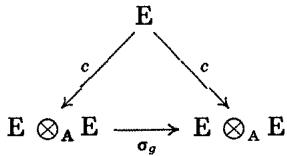
\includegraphics[keepaspectratio]{images/part004_b841500b.jpg}}

be commutative.

The proof is analogous to that of Proposition 2 of no. 2.

When the graded cogebra E satisfies the condition of Proposition 6, it is said to be anticocommutative.

Example. It follows immediately from formula (8) of no. 1 that for every A-module M, the graded cogebra \(\bigwedge(M)\) is anticocommutative.

\subsection{BIGEBRAS AND SKEW-BIGEBRAS}

DEFINITION 3. A graded bigebra (resp. skew graded bigebra) over a ring A is a set E with a graded A-algebra structure of type N and a graded A-cogebra structure of type N, with the same underlying graded A-module structure and such that:

\begin{enumerate}
\def\labelenumi{(\arabic{enumi})}
\item
  The A-algebra E is associative and unital.
\item
  The A-cogebra E is coassociative and counital.
\item
  The coproduct \(c: \mathbf{E} \to \mathbf{E} \otimes_{\mathbf{A}} \mathbf{E}\) is a homomorphism of the graded algebra \(\mathbf{E}\) into the graded algebra \(\mathbf{E} \otimes_{\mathbf{A}} \mathbf{E}\) (resp. graded algebra \(\mathbf{E}^{\mathfrak{g}} \otimes_{\mathbf{A}} \mathbf{E}\) (cf.~§ 4, no. 7)).
\item
  The counit \(\gamma\) of E is a homomorphism of the graded algebra E into the algebra A (with the trivial graduation) such that, if e denotes the unit element of the A-algebra \(\mathbf{E}, \gamma(e) = 1\) .
\end{enumerate}

If E is a graded bigebra whose graduation is trivial, E is called simply a bigebra. A graded bigebra is called commutative (resp. cocommutative) if the underlying algebra is commutative (resp. if the underlying cogebra is cocommutative); a skew graded bigebra is called anticommutative (resp. anticocommutative) if the underlying graded algebra is anticommutative (resp. if the underlying graded cogebra is anticocommutative).

It follows from Definition 3 and no. 2, Proposition 5 that, for a graded bigebra or a skew graded bigebra E,

\[
\left\{ \begin{array}{c} c (e) = e \otimes e \\ c (x) \equiv x \otimes e + e \otimes x (\mathrm{mod.} \mathrm{E} _ {+} \otimes \mathrm{E} _ {+}) \quad \text { for } x \in \mathrm{E} _ {+} = \bigoplus_ {n \geqslant 1} \mathrm{E} _ {n}. \end{array} \right.\tag{22}
\]

If E and F are two graded bigebras (resp. two skew graded bigebras), a mapping \(\phi: \mathrm{E} \to \mathrm{F}\) is called a graded bigebra morphism (resp. skew graded bigebra morphism) if: (1) \(\phi\) is a graded algebra morphism (and hence maps the unit element of E to the unit element of F); (2) \(\phi\) is a graded cogebra morphism such that, if \(\gamma\) and \(\gamma'\) are the respective counits of E and F, then \(\gamma = \gamma' \circ \phi\) .

Examples. (1) Let S be a monoid with identity element u, so that the algebra \(E = A^{(S)}\) of the monoid S over A admits the unit element \(e_{u}\) (§2, no. 6); it has been seen on the other hand that E has canonically a coassociative cocommutative A-cogebra structure with a counit \(\gamma\) such that \(\gamma(e_{s}) = 1\) for all \(s \in S\) (no. 1, Example 4 and no. 2, Examples 4, 5 and 6). The formula \(c(e_{s}) = e_{s} \otimes e_{s}\) giving the coproduct shows also immediately that c is an algebra homomorphism. Thus a cocommutative bigebra structure has been defined on E and E, with this structure, is called the bigebra of the monoid S over A.

If T is another monoid with unit element \(v, f: \mathrm{S} \to \mathrm{T}\) a homomorphism such that \(f(u) = v\) and \(f_{(\mathbf{A})}: \mathrm{A}^{(\mathrm{S})} \to \mathrm{A}^{(\mathrm{T})}\) the A-algebra homomorphism derived from \(f(\S 2, \text{no. } 6)\) , it is immediately verified that \(f_{(\mathbf{A})}\) is a bigebra homomorphism.

\begin{enumerate}
\def\labelenumi{(\arabic{enumi})}
\setcounter{enumi}{1}
\item
  Let M be an A-module. The graded A-algebra (§ 6, no. 1) and graded A-cogebra (no. 1, Example 6) structures defined on S(M) define on this set a commutative cocommutative graded bigebra structure; for we have seen (no. 1, Example 6) that the coproduct on S(M) is an algebra homomorphism and it follows from the definition of the counit \(\gamma\) (no. 2, Example 6) that \(\gamma(1) = 1\) and that \(\gamma\) is an algebra homomorphism of \(E\) into \(A\) .
\item
  Let M be an A-module. We see as in Example 2 that the graded A-algebra (§ 7, no. 1) and graded A-cogebra (no. 1, Example 7) structures on \(\bigwedge\) (M) define on this set an anticommutative anticocommutative skew graded bigebra structure.
\end{enumerate}

Remark. If M is an A-module such that \(M \otimes_{A} M \neq \{0\}\) , the graded A-algebra (§ 5, no. 1) and graded A-cogebra (no. 1, Example 5) structures on T(M) do not define a bigebra structure, for in general

\[
c (x _ {1} x _ {2} y _ {1} y _ {2}) \neq c (x _ {1} x _ {2}) c (y _ {1} y _ {2})
\]

for four elements \(x_{1}, x_{2}, y_{1}, y_{2}\) of M, as formula (3) of no. 1, shows.

\subsection{THE GRADED DUALS T(M)*gr, S(M)*gr AND ∧(M)*gr}

From now on we return to the general conventions of the chapter on algebras, which will therefore be assumed (unless otherwise mentioned) to be associative and unital.

Let M be an A-module; the graded A-cogebra structures defined on T(M) (no. 1, Example 5), S(M) (no. 1, Example 6) and \(\bigwedge\) (M) (no. 1, Example 7) allow us to define canonically on the graded duals T(M)*gr, S(M)*gr and \(\bigwedge\) (M)*gr graded algebra structures of type N, by virtue of no. 2, Propositions 1 and 3 and the convention made on the graduation of the graded dual of a graded module (no. 1). Moreover, the graded algebra S(M)*gr is commutative (no. 2, Proposition 2 and Example 5) and the graded algebra \(\bigwedge\) (M)*gr is anticommutative (no. 3, Proposition 6 and Example). In \(\bigwedge\) (M)*gr every element of degree 1 is of zero square; such an element is identified with a linear form \(f\) on M and its square is the alternating bilinear form \(f \wedge f\) on M \(^{2}\) such that

\[
(f \wedge f) (x, y) = f (x) f (y) - f (y) f (x)
\]

(no. 2, Example 3).

Let \(\mathbf{N}\) be another A-module and \(u\) an A-linear mapping of \(\mathbf{M}\) into \(\mathbf{N}\) . We know that \(u\) defines canonically graded algebra homomorphisms

\[
\left\{ \begin{array}{l} \mathsf {T} (u): \mathsf {T} (\mathbf {M}) \to \mathsf {T} (\mathbf {N}) \\ \mathsf {S} (u): \mathsf {S} (\mathbf {M}) \to \mathsf {S} (\mathbf {N}) \\ \bigwedge (u): \bigwedge (\mathbf {M}) \to \bigwedge (\mathbf {N}) \end{array} \right.\tag{23}
\]

(§ 5, no. 2, § 6, no. 2 and § 7, no. 2). It is immediately verified in formula (3) of no. 1 that \(\mathsf{T}(u)\) is also a cogebra morphism. On the other hand, if \(\Delta_{\mathbf{M}}\) (resp. \(\Delta_{\mathbf{N}}\) )

denotes the diagonal mapping \(\mathbf{M} \to \mathbf{M} \times \mathbf{M}\) (resp. \(\mathbf{N} \to \mathbf{N} \times \mathbf{N}\) ), there is the relation \((u \times u) \circ \Delta_{\mathbf{M}} = \Delta_{\mathbf{N}} \circ u\) ; it follows that \(\mathbf{S}(u \times u) \circ \mathbf{S}(\Delta_{\mathbf{M}}) = \mathbf{S}(\Delta_{\mathbf{N}}) \circ \mathbf{S}(u)\)

\[
(\text { resp. } \bigwedge (u \times u) \circ \bigwedge (\Delta_ {\mathbf {M}}) = \bigwedge (\Delta_ {\mathbf {N}}) \circ \bigwedge (u)).
\]

Using the definition of coproduct in \(\mathsf{S}(\mathbf{M})\) and \(\bigwedge (\mathbf{M})\) (no. 1, Examples 6 and 7) and the functorial character of the canonical isomorphisms

\[
\mathbf {S} (\mathbf {M} \times \mathbf {M}) \rightarrow \mathbf {S} (\mathbf {M}) \otimes_ {\mathbf {A}} \mathbf {S} (\mathbf {M})
\]

and \(\bigwedge (\mathbf{M}\times \mathbf{M})\to \bigwedge (\mathbf{M})^{\mathfrak{g}}\otimes_{\mathbf{A}}\bigwedge (\mathbf{M})\) , it is seen that \(S(u)\) and \(\bigwedge (u)\) are also cogebra morphisms† (and hence in this case bigebra morphisms). It follows immediately that the graded transposes (II, § 11, no. 6) of the homomorphisms (23)

\[
\begin{array}{c} ^ {t} \mathsf {T} (u): \mathsf {T} (\mathbf {N}) ^ {* \mathrm{gr}} \to \mathsf {T} (\mathbf {M}) ^ {* \mathrm{gr}} \\ ^ {t} \mathsf {S} (u): \mathsf {S} (\mathbf {N}) ^ {* \mathrm{gr}} \to \mathsf {S} (\mathbf {M}) ^ {* \mathrm{gr}} \\ ^ {t} \bigwedge (u): \bigwedge (\mathbf {N}) ^ {* \mathrm{gr}} \to \bigwedge (\mathbf {M}) ^ {* \mathrm{gr}} \end{array}
\]

are graded algebra homomorphisms.

We now note that the dual M* of M is identified with the submodule of elements of degree 1 in T(M)*gr (resp. S(M)*gr, ∧(M)*gr). It therefore follows from the universal property of the tensor algebra (§ 5, no. 1) and the universal property of the symmetric algebra (§ 6, no. 1) that there exists one and only one graded algebra homomorphism

\[
\theta_ {\mathsf {T}}: T (M ^ {*}) \rightarrow T (M) ^ {* \mathrm{gr}}
\]

which extends the canonical injection \(\mathbf{M}^{*}\to \mathsf{T}(\mathbf{M})^{*\mathrm{gr}}\) , and one and only one graded algebra homomorphism

\[
\theta_ {\mathsf {S}}: S (M ^ {*}) \rightarrow S (M) ^ {* \mathrm{gr}}
\]

which extends the canonical injection \(\mathbf{M}^{*}\to\mathsf{S}(\mathbf{M})^{*\mathrm{gr}}\) . On the other hand, the canonical injection of \(\mathbf{M}^{*}\) in the opposite algebra to \(\bigwedge(\mathbf{M})^{*\mathrm{gr}}\) is such that the square of every element of \(\mathbf{M}^{*}\) is zero; hence (§ 7, no. 1, Proposition 1) there exists one and only one graded algebra homomorphism

\[
\theta_ {\wedge}: \bigwedge (\mathbf {M} ^ {*}) \rightarrow (\bigwedge (\mathbf {M}) ^ {* \mathrm{gr}}) ^ {\circ}
\]

which extends the canonical injection \(M^{*}\to\bigwedge(M)^{*gr.}\) . These homomorphisms are functorial: for example, for every A-module homomorphism \(u:M\to N\) , the diagram

\pandocbounded{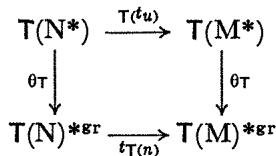
\includegraphics[keepaspectratio]{images/part004_1f4c9f33.jpg}}

is commutative, as follows immediately from the universal property of the tensor algebra (§ 5, no. 1); there are analogous commutative diagrams for \(\theta_{s}\) and \(\theta_{\wedge}\) .

We shall find the homomorphisms \(\theta_{\mathsf{T}}\) , \(\theta_{\mathsf{S}}\) and \(\theta_{\wedge}\) explicitly. For this we consider more generally a coassociative A-cogebra E with coproduct \(c\) and define by induction on \(n\) , for \(n \geqslant 2\) , the linear mapping \(c_{n}\) of E into \(\mathrm{E}^{\otimes n}\) by \(c_{2} = c\) and

\[
c _ {n} = \left(c _ {n - 1} \otimes 1 _ {\mathrm{E}}\right) \circ c.\tag{24}
\]

On the other hand we denote by \(m_{n}:A^{\otimes n}\to A\) the canonical linear mapping such that \(m_{n}(\xi_{1}\otimes\xi_{2}\otimes\cdots\otimes\xi_{n})=\xi_{1}\xi_{2}\ldots\xi_{n}\) and note that, for \(n\geqslant2\) ,

\[
m _ {n} = m \circ (m _ {n - 1} \otimes 1 _ {\mathbf {A}})\tag{25}
\]

writing \(m = m_2\) . With this notation:

Lemma 1. (i) In the associative algebra \(\mathbf{E}^* = \operatorname{Hom}_{\mathbf{A}}(\mathbf{E}, \mathbf{A})\) , the product of \(n\) elements \(u_1, u_2, \ldots, u_n\) of degree 1 is given by

\[
u _ {1} u _ {2} \dots u _ {n} = m _ {n} \circ (u _ {1} \otimes u _ {2} \otimes \dots \otimes u _ {n}) \circ c _ {n}.\tag{26}
\]

\begin{enumerate}
\def\labelenumi{(\roman{enumi})}
\setcounter{enumi}{1}
\tightlist
\item
  Suppose also that the cogebra E is graded. Then, in the graded associative algebra \(\mathbf{E}^{*\mathrm{gr}} = \operatorname{Homgr}_{\mathbf{A}}(\mathbf{E}, \mathbf{A})\) , the product of \(n\) elements \(u_1, u_2, \ldots, u_n\) of degree 1 is given by
\end{enumerate}

\[
u _ {1} u _ {2} \dots u _ {n} = m _ {n} \circ (u _ {1} \otimes u _ {2} \otimes \dots \otimes u _ {n}) \circ \delta_ {n}\tag{27}
\]

where \(\delta_n: \mathbf{E} \to \mathbf{E}^{\otimes n}\) is the linear mapping which maps each \(x \in \mathbf{E}\) to the component of \(c_n(x)\) of multidegree \((1, 1, \ldots, 1)\) .

Formula (26) is just the definition of the product in \(\mathbf{E}^*\) for \(n = 2\) ; to prove it by induction on \(n\) , observe that

\[
\begin{array}{l} u _ {1} u _ {2} \dots u _ {n} \\ \qquad = m \circ ((u _ {1} u _ {2} \dots u _ {n - 1}) \otimes u _ {n}) \circ c \\ \qquad = m \circ ((m _ {n - 1} \circ (u _ {1} \otimes u _ {2} \otimes \dots \otimes u _ {n - 1}) \circ c _ {n - 1}) \otimes u _ {n}) \circ c \\ \qquad = m \circ (m _ {n - 1} \otimes \mathrm{l} _ {\mathrm{A}}) \circ (u _ {1} \otimes u _ {2} \otimes \dots \otimes u _ {n - 1} \otimes u _ {n}) \circ (c _ {n - 1} \otimes \mathrm{l} _ {\mathrm{E}}) \circ c \\ \qquad = m _ {n} \circ (u _ {1} \otimes u _ {2} \otimes \dots \otimes u _ {n}) \circ c _ {n} \end{array}
\]

by virtue of (24), (25), II, § 3, no. 3, formula (5) and the relation

\[
u _ {n} = 1 _ {\mathbf {A}} \circ u _ {n} \circ 1 _ {\mathbf {E}}.
\]

When E is graded and the elements \(u_{i} \in E^{*gr}\) homogeneous of degree 1, then by definition for homogeneous elements \(x_{i} \in E\) ,

\[
(u _ {1} \otimes u _ {2} \otimes \dots \otimes u _ {n}) (x _ {1} \otimes x _ {2} \otimes \dots \otimes x _ {n}) = 0
\]

unless all the \(x_{i}\) are of degree 1, whence formula (27).

It follows from formulae (3), (5) and (7) of no. 1 and formula (24) that when E is taken to be one of the three graded cogebras \(\mathsf{T}(\mathbf{M})\) , \(\mathsf{S}(\mathbf{M})\) and \(\bigwedge (\mathbf{M})\) , we obtain respectively by induction on \(n\) (using the fact that the coproduct is a graded homomorphism of degree 0), for \(x_{1}, x_{2}, \ldots, x_{n}\) in M:

\[
\text { when   } \mathrm{E} = \mathrm{T} (\mathrm{M}), \quad \delta_ {n} (x _ {1} x _ {2} \dots x _ {n}) = x _ {1} \otimes x _ {2} \otimes \dots \otimes x _ {n}
\]

\[
\text { when } \mathrm{E} = \mathrm{S(M)}, \quad \delta_ {n} (x _ {1} x _ {2} \dots x _ {n}) = \sum_ {\sigma \in \mathfrak {S} _ {n}} x _ {\sigma (1)} \otimes x _ {\sigma (2)} \otimes \dots \otimes x _ {\sigma (n)}
\]

\[
\text { when } \mathrm{E} = \bigwedge (\mathrm{M}), \quad \delta_ {n} (x _ {1} x _ {2} \dots x _ {n}) = \sum_ {\sigma \in \mathfrak {S} _ {n}} \varepsilon_ {\sigma}. x _ {\sigma (1)} \otimes x _ {\sigma (2)} \otimes \dots \otimes x _ {\sigma (n)}.
\]

It suffices to note, for example when \(\mathbf{E} = \bigwedge (\mathbf{M})\) , that in the expression \(c_{n}(x_{1}x_{2}\ldots x_{n}) = (c_{n - 1}\otimes 1_{\mathbb{E}})\left(\sum (-1)^{\nu}(x_{i_1}\ldots x_{i_p})\otimes (x_{j_1}\ldots x_{j_{n - p}})\right)\) arising from formula (8) of no. 1, the only terms which can give a term of multidegree \((1,1,\dots ,1)\) are those for which \(n - p = 1\) and hence

\[
\delta_ {n} (x _ {1} x _ {2} \dots x _ {n})
\]

is the term of multidegree \((1, 1, \ldots, 1)\) in the sum

\[
\sum_ {i = 1} ^ {n} (- 1) ^ {n - i} c _ {n - 1} \left(x _ {1} \dots x _ {i - 1} x _ {i + 1} \dots x _ {n}\right) \otimes x _ {i}
\]

and this term is necessarily equal to

\[
\sum_ {i = 1} ^ {n} (- 1) ^ {n - i} \delta_ {n - 1} (x _ {1} \dots x _ {i - 1} x _ {i + 1} \dots x _ {n}) \otimes x _ {i},
\]

whence the result by the induction hypothesis.

Using Lemma 1, the product in \(\mathsf{T}(\mathbf{M})^{*\mathrm{gr}}\) of \(n\) linear forms \(x_{1}^{*}, x_{2}^{*}, \ldots, x_{n}^{*}\) of \(\mathbf{M}^{*}\) is given by

\[
\left\langle x _ {1} ^ {*} x _ {2} ^ {*} \dots x _ {n} ^ {*}, x _ {1} x _ {2} \dots x _ {n} \right\rangle = \prod_ {i = 1} ^ {n} \left\langle x _ {i} ^ {*}, x _ {i} \right\rangle\tag{28}
\]

for \(x_{i} \in \mathbf{M} (1 \leqslant i \leqslant n)\) ; the product of these \(n\) forms in \(S(M)^{*gr}\) is given by

\[
\left\langle x _ {1} ^ {*} x _ {2} ^ {*} \dots x _ {n} ^ {*}, x _ {1} x _ {2} \dots x _ {n} \right\rangle = \sum_ {\sigma \in \mathfrak {S} _ {n}} \left(\prod_ {i = 1} ^ {n} \left\langle x _ {\sigma (i)} ^ {*}, x _ {i} \right\rangle\right);\tag{29}
\]

finally, the product of these forms in \(\bigwedge (\mathbf{M})^{*\mathrm{gr}}\) is given by

\[
\langle x _ {1} ^ {*} x _ {2} ^ {*} \dots x _ {n} ^ {*}, x _ {1} x _ {2} \dots x _ {n} \rangle = \det (\langle x _ {i} ^ {*}, x _ {j} \rangle).\tag{30}
\]

In each of the three cases, we have respectively

\[
\theta_ {T} (x _ {1} ^ {*} \otimes x _ {2} ^ {*} \otimes \dots \otimes x _ {n} ^ {*}) = x _ {1} ^ {*} x _ {2} ^ {*} \dots x _ {n} ^ {*}
\]

\[
\theta_ {S} (x _ {1} ^ {*} x _ {2} ^ {*} \dots x _ {n} ^ {*}) = x _ {1} ^ {*} x _ {2} ^ {*} \dots x _ {n} ^ {*}
\]

\[
\theta_ {\wedge} (x _ {1} ^ {*} \wedge x _ {2} ^ {*} \wedge \dots \wedge x _ {n} ^ {*}) = x _ {n} ^ {*} x _ {n - 1} ^ {*} \dots x _ {1} ^ {*} = (- 1) ^ {n (n - 1) / 2} x _ {1} ^ {*} x _ {2} ^ {*} \dots x _ {n} ^ {*}
\]

and hence we deduce from (28), (29) and (30) the relations

\[
\langle \theta_ {T} (x _ {1} ^ {*} \otimes x _ {2} ^ {*} \otimes \dots \otimes x _ {n} ^ {*}), x _ {1} \otimes x _ {2} \otimes \dots \otimes x _ {n} \rangle = \prod_ {i = 1} ^ {n} \langle x _ {i} ^ {*}, x _ {i} \rangle\tag{28 bis}
\]

(in other words \(\theta_{\mathsf{T}}\) restricted to \(\mathsf{T}^2 (\mathbf{M}^*)\) is just the canonical homomorphism of II, § 4, no. 4)

\[
\langle \theta_ {\mathsf {S}} (x _ {1} ^ {*} x _ {2} ^ {*} \dots x _ {n} ^ {*}), x _ {1} x _ {2} \dots x _ {n} \rangle = \sum_ {\sigma \in \mathfrak {S} _ {n}} \left(\prod_ {i = 1} ^ {n} \langle x _ {\sigma (i)} ^ {*}, x _ {i} \rangle\right)\tag{29 bis}
\]

\[
\begin{array}{r l} (30 \text { bis}) &\langle \theta_ {\wedge} (x _ {1} ^ {*} \wedge x _ {2} ^ {*} \wedge \dots \wedge x _ {n} ^ {*}), x _ {1} \wedge x _ {2} \wedge \dots \wedge x _ {n} \rangle \\ & \qquad = (- 1) ^ {n (n - 1) / 2} \mathrm{det} (\langle x _ {i} ^ {*}, x _ {j} \rangle). \end{array}
\]

PROPOSITION 7. Let \(\mathbf{M}\) be a finitely generated projective A-module. Then the canonical homomorphisms \(\theta_{\mathsf{T}}: \mathsf{T}(\mathbf{M}^{*}) \to \mathsf{T}(\mathbf{M})^{*\mathrm{gr}}\) and \(\theta_{\wedge}: \bigwedge (\mathbf{M}^{*}) \to (\bigwedge (\mathbf{M})^{*\mathrm{gr}})^{0}\) are bijective. Also the graded dual \(\bigwedge (\mathbf{M})^{*\mathrm{gr}}\) is then equal to the dual \(\bigwedge (\mathbf{M})^{*}\) of the A-module \(\bigwedge (\mathbf{M})\) .

Suppose first that \(\mathbf{M}\) has a finite basis \((e_i)_{1\leq i\leq m}\) and let \((e_i^*)_{1\leq i\leq m}\) be the dual basis of \(\mathbf{M}^*\) (II, § 10, no. 4). Formula (28 bis) shows that, for every finite sequence \(s = (j_k)_{1\leq k\leq n}\) of \(n\) elements of the interval \([1,m]\) of \(\mathbf{N}\) ,

\[
\theta_ {\mathsf {T}} (e _ {j _ {1}} ^ {*} \otimes \dots \otimes e _ {j _ {n}} ^ {*})
\]

is the element of index \(s\) in the basis of \((\mathsf{T}^n (\mathbf{M}))^*\) , dual to the basis of \(\mathsf{T}^n (\mathbf{M})\) consisting of the \(e_s = e_{j_1}\otimes \dots \otimes e_{j_n}\) (§ 5, no. 5, Theorem 1). Hence \(\theta_{\mathsf{T}}\) is bijective.

Similarly, formula (30 bis) shows that, for every finite subset \(\mathbf{H}\) of \([1, m]\) with \(n\) elements, \((-1)^{n(n-1)/2} \theta_{\wedge}(e_{\mathrm{H}}^{*})\) (notation of §7, no. 8, Theorem 1) is the element of index \(\mathbf{H}\) in the basis of \((\bigwedge^{n}(\mathbf{M}))^{*}\) , dual to the basis of \(\bigwedge^{n}(\mathbf{M})\) consisting of the \(e_{\mathrm{H}}\) . Hence \(\theta_{\wedge}\) is bijective.

Suppose now only that M is finitely generated and projective; then M is a direct factor of a finitely generated free A-module L, so that there exist two

A-linear mappings \(M \xrightarrow{j} L \xrightarrow{p} M\) whose composition is the identity \(1_{M}\) . We deduce a commutative diagram

\pandocbounded{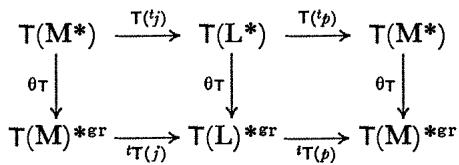
\includegraphics[keepaspectratio]{images/part004_2d3cbe02.jpg}}

and an analogous commutative diagram where \(\mathsf{T}\) is replaced by \(\bigwedge\) . The proposition then follows from the following lemma:

Lemma 2. Let

\pandocbounded{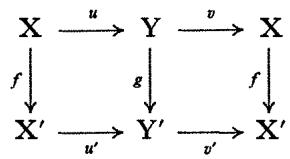
\includegraphics[keepaspectratio]{images/part004_a09507a7.jpg}}

be a commutative diagram of sets and mappings such that \(v \circ u\) and \(v' \circ u'\) are the identity mappings of \(X\) and \(X'\) respectively. Then, if \(g\) is injective (resp. surjective, resp. bijective), so is \(f\) .

u is injective since \(v \circ u\) is, hence, if g is injective, \(u' \circ f = g \circ u\) is injective and therefore f is injective. Similarly \(v'\) is surjective since \(v' \circ u'\) is; hence, if g is surjective, \(f \circ v = v' \circ g\) is surjective and therefore f is surjective.

The last assertion of Proposition 7 follows from the fact that \(\bigwedge (\mathbf{M})\) is then a finitely generated A-module (§ 7, no. 3, Proposition 6 and II, § 11, no. 6, Remark).

We now examine what can be said concerning the homomorphism \(\theta_{\mathsf{S}}\) when \(\mathbf{M}\) is projective and finitely generated. Suppose first that \(\mathbf{M}\) admits a finite basis \((e_i)_{1\leq i\leq m}\) . In the notation at the beginning of the chapter the A-module \(\mathbf{S}^n (\mathbf{M})\) admits as basis the family of elements \(e^{\alpha}\) such that \(|\alpha | = n\) . Let \(u_{\alpha}\) (for \(|\alpha | = n\) ) denote the element of index \(\alpha\) in the basis of \((\mathbf{S}^n (\mathbf{M}))^*\) dual to \((e^{\alpha})\) . The elements \(u_{\alpha}\) , for \(\alpha \in \mathbf{N}^m\) , therefore form a basis of the algebra \(\mathbf{S}(\mathbf{M})^{*\mathrm{gr}}\) and we shall obtain the multiplication table of this basis explicitly. We write

\[
u _ {\alpha} u _ {\beta} = \sum_ {\gamma \in \mathbf {N} ^ {m}} a _ {\alpha \beta \gamma} u _ {\gamma} \quad \text { with } a _ {\alpha \beta \gamma} \in \mathrm{A}.
\]

Then by definition

\[
a _ {\alpha \beta \gamma} = \langle u _ {\alpha} u _ {\beta}, e ^ {\gamma} \rangle = m ((u _ {\alpha} \otimes u _ {\beta}) (c (e ^ {\gamma}))),
\]

where \(m: \mathbf{A} \otimes \mathbf{A} \to \mathbf{A}\) defines the multiplication on \(\mathbf{A}\) and \(c\) is the coproduct of \(\mathsf{S}(\mathbf{M})\) . In other words, \(a_{\alpha \beta \gamma}\) is just the coefficient of \(e^{\alpha} \otimes e^{\beta}\) when \(c(e^{\gamma})\) is written in terms of the basis of \(\mathsf{S}(\mathbf{M})\otimes \mathsf{S}(\mathbf{M})\) consisting of the \(e^{\xi}\otimes e^{\eta}\) , where \(\xi\) and \(\eta\) run through \(\mathbf{N}^m\) . But since \(c\) is an algebra homomorphism,

\[
c (e ^ {\gamma}) = \prod_ {i = 1} ^ {m} (c (e _ {i})) ^ {\gamma_ {i}} = \prod_ {i = 1} ^ {m} (e _ {i} \otimes 1 + 1 \otimes e _ {i}) ^ {\gamma_ {i}}
\]

by formula (4) of no. 1; this gives

\[
c (e ^ {\gamma}) = \sum_ {\xi + \eta = \gamma} (\xi , \eta) e ^ {\xi} \otimes e ^ {\eta}\tag{31}
\]

where we write

\[
((\xi , \eta)) = \prod_ {i = 1} ^ {n} \frac {(\xi_ {i} + \eta_ {i}) !}{\xi_ {i} ! \eta_ {i} !} \quad (\text { cf.   } \S 10, \text {   no.   } 4, \text {   formula   (18) }).\tag{32}
\]

Hence we obtain the multiplication table

\[
u _ {\alpha} u _ {\beta} = ((\alpha , \beta)) u _ {\alpha + \beta}.\tag{33}
\]

On the other hand, if \((e_i^*)_{1\leq i\leq m}\) is the basis of \(\mathbf{M}^*\) , dual to \((e_i)\) , it follows from formula (29 bis) that, for all \(\alpha \in \mathbf{N}^m\) ,

\[
\theta_ {S} (e ^ {* \alpha}) = \alpha ! u _ {\alpha}\tag{34}
\]

in the notation of § 6, no. 6. Hence the homomorphism \(\theta_{\mathsf{S}}\) is bijective if and only if the \(\alpha!u_{\alpha}\) form a basis of \(\mathsf{S}(\mathbf{M})^{*\mathrm{gr}}\) , or also if the elements \(\alpha!1\) are invertible.

PROPOSITION 8. Suppose that the ring A is an algebra over the field Q of rational numbers; then, for every finitely generated projective A-module M, the homomorphism

\[
\theta_ {\mathsf {S}}: S (M ^ {*}) \rightarrow S (M) ^ {* \mathrm{gr}}
\]

is bijective.

It amounts to proving this when M is finitely generated and free; we pass from this to the general case using Lemma 2 as in the proof of Proposition 7.

Remark. Let M be an A-module and \(\rho: \mathbf{A} \to \mathbf{B}\) a commutative ring homomorphism. Then there is a commutative diagram of graded B-algebra homomorphisms

\[
\begin{array}{l} \mathsf {T} ((\mathbf {M} ^ {*}) _ {(B)}) \longrightarrow (\mathsf {T} (\mathbf {M}) ^ {* \mathrm{gr}}) _ {(B)} \\ \mathsf {T} (\upsilon_ {\mathbf {M}}) \Biggl \downarrow \qquad \qquad \qquad \qquad \qquad \qquad \qquad \qquad \qquad \Biggl \downarrow \upsilon_ {\mathbf {T} (\mathbf {M})} \\ \mathsf {T} ((\mathbf {M} _ {(B)}) ^ {*}) \xrightarrow [ \theta_ {\mathsf {T}} ]{} \mathsf {T} (\mathbf {M} _ {(B)}) ^ {* \mathrm{gr}} \end{array}
\]

where the first row is a homomorphism composed of the homomorphism \(\theta_{\mathsf{T}}\otimes 1_{\mathsf{B}}\colon \mathsf{T}(\mathbf{M}^{*})\otimes_{\mathbf{A}}\mathbf{B}\to \mathsf{T}(\mathbf{M})^{*\mathrm{gr}}\) and the canonical isomorphism

\[
\mathsf {T} ((\mathbf {M} ^ {*}) _ {(\mathbf {B})}) \rightarrow \mathsf {T} (\mathbf {M} ^ {*}) \otimes_ {\mathbf {A}} \mathbf {B}
\]

(§ 5, no. 3, Proposition 5). It is immediately verified, using formula (28) and the definition of the homomorphism \(\upsilon_{\mathbf{E}}\) (II, § 5, no. 4), that this diagram is commutative. When \(\mathbf{M}\) is a finitely generated projective A-module, \(\mathbf{M}_{(\mathbf{B})}\) is a finitely generated projective B-module (II, § 5, no. 1, Corollary to Proposition 4) and all the homomorphisms of the above diagram are bijective (Proposition 7 and II, § 5, no. 4, Proposition 8). There are analogous commutative diagrams with \(\mathsf{T}\) replaced by \(\mathsf{S}\) or \(\bigwedge\) ; the diagram for \(\bigwedge\) also consists of bijective homomorphisms when \(\mathbf{M}\) is projective and finitely generated (Proposition 7); if further \(\mathbf{A}\) is an algebra over \(\mathbf{Q}\) , the diagram for \(\mathsf{S}\) also consists of bijective homomorphisms (Proposition 8).

\subsection{INNER PRODUCTS: CASE OF ALGEBRAS}

Let \(E = \bigoplus_{p \geqslant 0} E_p\) be a graded A-algebra of type N and P a graded A-module of type Z; for every homogeneous element \(x \in E_p\) , left multiplication by \(x\) is an A-linear mapping \(e(x)\) of E into itself which is graded of degree \(p\) . For every element \(u \in \text{Homgr}_A(E, P)\) , the right inner product of \(u\) by \(x\) , denoted by \(u \llcorner x\) , is the element \(u \circ e(x)\) of \(\text{Homgr}_A(E, P)\) . We also write \((i(x))(u) = u \llcorner x\) and we see that \(i(x)\) is a graded endomorphism of degree \(p\) of the graded A-module \(\text{Homgr}_A(E, P)\) . If now \(x = \sum_{p \geqslant 0} x_p\) is an arbitrary element of E (with \(x_p \in E_p\) for all \(p \geqslant 0\) , \(x_p = 0\) except for a finite number of values of \(p\) ), we write \(i(x) = \sum_{p=0}^{\infty} i(x_p)\) , which is therefore an endomorphism of the A-module \(\text{Homgr}_A(E, P)\) .

To remember which element, in the expression \(u \llcorner x\) , ``operates'' on the other, observe that the element x which ``operates'' on u is placed at the free end of the horizontal line in \(\llcorner\).

The associativity of the algebra E goes over to the relation \(e(xy) = e(x) \circ e(y)\) for x, y homogeneous; whence, by definition of \(i(x)\) ,

\[
i (x y) = i (y) \circ i (x)\tag{35}
\]

first for \(x, y\) homogeneous and then, by linearity, for arbitrary \(x, y\) in E; this may also be written

\[
(u \llcorner x) \llcorner y = u \llcorner (x y)\tag{36}
\]

for \(x, y\) in \(\mathbf{E}\) and \(u \in \operatorname{Homgr}_{\mathbf{A}}(\mathbf{E}, \mathbf{P})\) ; as on the other hand clearly \(i(1)\) is the identity mapping (since this follows from \(e(1) = 1_{\mathbf{E}}\) ) and \(x \mapsto i(x)\) is A-linear, it is seen that the external law of composition \((x, u) \mapsto u \llcorner x\) ( \(x \in \mathbf{E}\) , \(u \in \operatorname{Homgr}_{\mathbf{A}}(\mathbf{E}, \mathbf{P})\) ) defines, with addition, a right E-module structure on \(\operatorname{Homgr}_{\mathbf{A}}(\mathbf{E}, \mathbf{P})\) .

In particular we consider the case P = A, \(\operatorname{Homgr}_{\mathbf{A}}(\mathbf{E}, \mathbf{P})\) being in this case the graded dual \(E^{*gr}\) of E; \(i(x)\) is then the graded transpose of the A-linear mapping \(e(x)\) (II, §11, no. 6), in other words, for all x, y in E, \(u \in E^{*gr}\) ,

\[
\langle u \llcorner x, y \rangle = \langle u, x y \rangle .\tag{37}
\]

With the convention at the beginning of the paragraph, note that, if \(x \in E_{p}\) , \(i(x)\) is an endomorphism of \(E^{*gr}\) of degree -p.

For every homogeneous element \(x \in \mathbf{E}_p\) , right multiplication by \(x\) is similarly denoted by \(e'(x)\) and the element \(u \circ e'(x)\) of \(\operatorname{Homgr}_{\mathbf{A}}(\mathbf{E}, \mathbf{P})\) , called the left inner product of \(u\) by \(x\) , by \(x \lrcorner u\) ; we write \(i'(x) = x \lrcorner u\) and \(i'(x)\) is therefore a graded endomorphism of \(\operatorname{Homgr}_{\mathbf{A}}(\mathbf{E}, \mathbf{P})\) of degree \(p\) ; as above this definition can be extended to the case where \(x\) is an arbitrary element of \(\mathbf{E}\) . As in this case \(e'(xy) = e'(y)e'(x)\) ,

\[
i ^ {\prime} (x y) = i ^ {\prime} (x) \circ i ^ {\prime} (y)\tag{38}
\]

which may also be written

\[
x \lrcorner (y \lrcorner u) = (x y) \lrcorner u\tag{39}
\]

and shows that the external law of composition \((x,u)\mapsto x\lrcorner u\) defines, with addition, a left E-module structure on \(\operatorname{Homgr}_{\mathbf{A}}(\operatorname{E},\operatorname{P})\) . The associativity of E implies on the other hand that \(e(x)\circ e'(y)=e'(y)\circ e(x)\) for x,y homogeneous in E, whence the relation

\[
(y \lrcorner u) \llcorner x = y \lrcorner (u \llcorner x)\tag{40}
\]

so that the two external laws of composition on \(\mathrm{Homgr}_{\mathbf{A}}(\mathbf{E},\mathbf{P})\) define on this set an (E, E)-bimodule structure (II, § 1, no. 14).

When we take \(\mathbf{P} = \mathbf{A}\) , \(i'(x)\) is the graded transpose of \(e'(x)\) ; in other words, for all \(x, y\) in \(\mathbf{E}\) , \(u \in \mathbf{E}^{*\mathrm{gr}}\) ,

\[
\langle y, x \lrcorner u \rangle = \langle y x, u \rangle .\tag{41}
\]

When the graded algebra E is commutative, obviously \(u \llcorner x = x \lrcorner u\) . When E is anticommutative and P = A, then for \(x \in E_{p}\) , \(y \in E_{r}\) and \(u \in E_{q}^{*}\) , \(yx = (-1)^{pr}xy\) , whence, by (37) and (41), \(\langle u \llcorner x, y \rangle = (-1)^{pr}\langle y, x \lrcorner u \rangle\) . But as the two sides of this relation are zero except for r = q - p,

\[
x \lrcorner u = (- 1) ^ {p (q - p)} u \llcorner x.
\]

Let F be another graded A-algebra and \(\phi: E \to F\) an A-homomorphism of graded algebras; then \(\tilde{\phi} = \operatorname{Hom}(\phi, 1_{P}): \operatorname{Homgr}_{A}(F, P) \to \operatorname{Homgr}_{A}(E, P)\) is a graded A-homomorphism of degree 0; by definition, for \(x, y\) in E and \(u \in \operatorname{Homgr}_{A}(F, P)\)

\[
\begin{array}{r l} (\tilde {\phi} (u \llcorner \phi (x))) (y) & = (u \llcorner \phi (x)) (\phi (y)) \\ & = u (\phi (x) \phi (y)) = u (\phi (x y)) = (\tilde {\phi} (u)) (x y) = (\tilde {\phi} (u) \llcorner x) (y) \end{array}
\]

or also

\[
\tilde {\phi} (u \llcorner \phi (x)) = \tilde {\phi} (u) \llcorner x\tag{42}
\]

and similarly

\[
\tilde {\phi} (\phi (x) \lrcorner u) = x \lrcorner \tilde {\phi} (u).\tag{43}
\]

In other words, when \(\operatorname{Homgr}_{\mathbf{A}}(\mathbf{F}, \mathbf{P})\) is considered as an (E, E)-bimodule by means of the ring homomorphism \(\phi: \mathbf{E} \to \mathbf{F}\) , it is seen that \(\tilde{\phi}\) is an (E, E)-bimodule homomorphism (or also an E-homomorphism of the (F, F)-bimodule \(\operatorname{Homgr}_{\mathbf{A}}(\mathbf{F}, \mathbf{P})\) into the (E, E)-bimodule \(\operatorname{Homgr}_{\mathbf{A}}(\mathbf{E}, \mathbf{P})\) ).

Examples. In particular the above may be applied when E is one of the graded algebras \(\mathsf{T}(\mathbf{M})\) , \(\mathsf{S}(\mathbf{M})\) or \(\bigwedge(\mathbf{M})\) for an A-module M and P an A-module (with the trivial graduation). To find explicitly the bimodule structures thus obtained, note that the elements of degree -n of \(\operatorname{Homgr}_{\mathbf{A}}(\mathsf{T}(\mathbf{M}),\mathbf{P})\) (resp. \(\operatorname{Homgr}_{\mathbf{A}}(\mathsf{S}(\mathbf{M}),\mathbf{P})\) , resp. \(\operatorname{Homgr}_{\mathbf{A}}(\bigwedge(\mathbf{M}),\mathbf{P})\) ) are identified with the n-linear mappings (resp. symmetric n-linear mappings, resp. alternating n-linear mappings) of \(M^{n}\) into P. It suffices to express the products

\[
f \llcorner (x _ {1} \otimes x _ {2} \otimes \dots \otimes x _ {p})
\]

\((\text{resp. } f \llcorner (x_1 x_2 \ldots x_p), \text{ resp. } f \llcorner (x_1 \wedge x_2 \wedge \dots \wedge x_p))\) for every finite sequence \((x_i)_{1 \leq i \leq p}\) of elements of M and the analogues for the left inner product. It follows immediately from the definitions that

\[
f \llcorner (x _ {1} \otimes x _ {2} \otimes \dots \otimes x _ {p}) = (x _ {1} \otimes x _ {2} \otimes \dots \otimes x _ {p}) \lrcorner f = 0\tag{44}
\]

if \(p > n\) and that, for \(p \leqslant n, f \llcorner (x_1 \otimes x_2 \otimes \dots \otimes x_p)\) (resp.

\[
\left(x _ {1} \otimes x _ {2} \otimes \dots \otimes x _ {p}\right) \lrcorner f)
\]

is the \((n - p)\) -linear mapping defined by

\[
\left\{ \begin{array}{l} (f \llcorner (x _ {1} \otimes x _ {2} \otimes \dots \otimes x _ {p})) (y _ {1}, \ldots , y _ {n - p}) \\ = f (x _ {1}, \ldots , x _ {p}, y _ {1}, \ldots , y _ {n - p}) \\ ((x _ {1} \otimes x _ {2} \otimes \dots \otimes x _ {p}) \lrcorner f) (y _ {1}, \ldots , y _ {n - p}) \\ = f (y _ {1}, \ldots , y _ {n - p}, x _ {1}, \ldots , x _ {p}). \end{array} \right.\tag{45}
\]

For \(p > n\) , there are also in \(\operatorname{Homgr}_{\mathbf{A}}(\mathsf{S}(\mathbf{M}), \mathbf{P})\) (resp. \(\operatorname{Homgr}_{\mathbf{A}}(\bigwedge(\mathbf{M}), \mathbf{P})\) ) formulae (44) with \(x_1 \otimes x_2 \otimes \cdots \otimes x_p\) replaced by \(x_1x_2 \ldots x_p\) (resp. \(x_1 \wedge x_2 \wedge \cdots \wedge x_p\) ). For \(p \leqslant n\) , the same substitutions in (45) define the symmetric \((n - p)\) -linear mappings \(f \llcorner (x_1x_2 \ldots x_p)\) and \((x_1x_2 \ldots x_p) \lrcorner f\) (resp. the alternating \((n - p)\) -linear mappings

\[
f \llcorner (x _ {1} \wedge x _ {2} \wedge \dots \wedge x _ {p}) \quad \text { and } \quad (x _ {1} \wedge x _ {2} \wedge \dots \wedge x _ {p}) \lrcorner f).
\]

When \(n = p\) , the above products are equal to the constant function on \(\mathbf{M}\) equal to \(f(x_{1},\ldots ,x_{p})\) .

If \(u: \mathbf{M} \to \mathbf{N}\) is an A-module homomorphism, \(\mathsf{T}(u): \mathsf{T}(\mathbf{M}) \to \mathsf{T}(\mathbf{N})\) is a graded A-algebra homomorphism, then it follows from what we have seen above that \((\mathsf{T}(u))^{\sim}\) is a \(\mathsf{T}(\mathbf{M})\) -homomorphism of the \((\mathsf{T}(\mathbf{N}), \mathsf{T}(\mathbf{N}))\) -bimodule \(\operatorname{Homgr}_{\mathbf{A}}(\mathsf{T}(\mathbf{N}), \mathbf{P})\) into the \((\mathsf{T}(\mathbf{M}), \mathsf{T}(\mathbf{M}))\) -bimodule \(\operatorname{Homgr}_{\mathbf{A}}(\mathsf{T}(\mathbf{M}), \mathbf{P})\) , relative to the ring homomorphism \(\mathsf{T}(u)\) . There are analogous results for \((\mathbf{S}(u))^{\sim}\) and \((\bigwedge(u))^{\sim}\) .

\subsection{INNER PRODUCTS: CASE OF COGEBRAS}

Let \(E = \bigoplus_{p \geq 0} E_p\) be a coassociative counital graded cogebra. Then we know (no. 2, Propositions 1 and 3) that the graded dual \(E^{*gr}\) has (with the convention on graduations made at the beginning of the paragraph) a graded algebra structure of type N over A, the product of two elements \(u, v\) of this algebra being defined by \(uv = m \circ (u \otimes v) \circ c\) , where \(c: E \to E \otimes_A E\) is the coproduct and \(m: A \otimes_A A \to A\) defines the multiplication. In other words, if, for \(x \in E\) , \(c(x) = \sum_i y_i \otimes z_i\) , we can write (canonically identifying \(A \otimes_A E\) and \(E\) )

\[
\begin{array}{r l} \langle x, u v \rangle = (u v) (x) & = \sum_ {i} u (y _ {i}) v (z _ {i}) = v \left(\sum_ {i} u (y _ {i}) z _ {i}\right) \\ & = v (((u \otimes 1 _ {\mathbb {E}}) \circ c) (x)) = \langle ((u \otimes 1 _ {\mathbb {E}}) \circ c) (x), v \rangle . \end{array}
\]

This can be interpreted by saying that, for all u homogeneous of degree p in \(E^{*gr}\) , the left multiplication \(e(u): v \mapsto uv\) in \(E^{*gr}\) is the graded transpose of the graded endomorphism of degree -p

\[
i (u) = (u \otimes 1 _ {\mathrm{E}}) \circ c\tag{46}
\]

of E; hence, in the above notation,

\[
(i (u)) (x) = \sum_ {i} u (y _ {i}) z _ {i}.
\]

Formula (46) also defines an element \(i(u)\in\mathrm{Endgr}_{\mathbf{A}}(\mathbf{E})\) for every element \(u\in\mathbf{E}^{*\mathbf{g}\mathbf{r}}\) ; for all \(x\in\mathbf{E}\) and all \(u\in\mathbf{E}^{*\mathbf{g}\mathbf{r}}\) , we write

\[
x \llcorner u = (i (u)) (x)\tag{47}
\]

so that, for u and v in E*gr,

\[
\langle x, u v \rangle = \langle x \llcorner u, v \rangle .
\]

The element \(x \llcorner u\) of E is called the right inner product of x by u.

Here again the element u which ``operates'' on x is placed at the free end of the horizontal line in L.

For any two elements \(u, v\) of \(\mathbf{E}^{*\mathrm{gr}}\) ,

\[
x \llcorner (u v) = (x \llcorner u) \llcorner v,\tag{48}
\]

in other words

\[
i (u v) = i (v) \circ i (u).
\]

As above let \(c(x) = \sum_{i} y_{i} \otimes z_{i}\) , so that \(x \llcorner (uv) = \sum_{i} (uv)(y_{i})z_{i}\) . If

\[
c (y _ {i}) = \sum_ {j} y _ {i j} ^ {\prime} \otimes y _ {i j} ^ {\prime \prime},
\]

then

\[
x \llcorner (u v) = \sum_ {i, j} u \left(y _ {i j} ^ {\prime}\right) v \left(y _ {i j} ^ {\prime \prime}\right) z _ {i}.\tag{49}
\]

On the other hand, if \(c(z_{i}) = \sum_{k} z_{ik}' \otimes z_{ik}''\) , then

\[
(x \llcorner u) \llcorner v = \sum_ {i, k} u (y _ {i}) v (z _ {i k} ^ {\prime}) z _ {i k} ^ {\prime \prime}.\tag{50}
\]

Now, the coassociativity of E shows that (no. 2, Proposition 1)

\[
\sum_ {i, j} y _ {i j} ^ {\prime} \otimes y _ {i j} ^ {\prime \prime} \otimes z _ {i} = \sum_ {i, k} y _ {i} \otimes z _ {i k} ^ {\prime} \otimes z _ {i k} ^ {\prime \prime}\tag{51}
\]

and the equality of expressions (49) and (50) follows from the fact that they are respectively the image of the left and right hand sides of (51) under the linear mapping f from \(E \otimes E \otimes E\) to E such that \(f(x \otimes y \otimes z) = u(x)v(y)z\) .

We recall on the other hand (no. 2, Proposition 3) that the unit element of the algebra \(\mathbf{E}^{*\mathrm{gr}}\) is the linear form \(e: x \mapsto \gamma(x).1\) ; hence

\[
x \llcorner e = \sum_ {i} \gamma (y _ {i}) z _ {i} = x
\]

by virtue of the definition of counit. As the mapping \(u \mapsto i(u)\) is linear, it is seen that the external law of composition \((u, x) \mapsto x \llcorner u\) defines a right E*gr-module structure on E.

Similarly we define, for all \(u \in \mathrm{E}^{*\mathbf{g}\mathbf{r}}\) , the endomorphism of \(\mathbf{E}\)

\[
i ^ {\prime} (u) = \left(1 _ {E} \otimes u\right) \circ c\tag{52}
\]

and, for all \(x \in \mathbf{E}\) , we write

\[
\left(i ^ {\prime} (u)\right) (x) = u \lrcorner x\tag{53}
\]

and this element of E is called the left inner product of x by u. As above it is seen that the external law \((u, v) \mapsto u \lrcorner x\) defines a left \(\mathrm{E}^{*gr}\) -module structure on E. Moreover, these two structures are compatible, in other words,

\[
(u \lrcorner x) \llcorner v = u \lrcorner (x \llcorner v)\tag{54}
\]

for \(u, v\) in E*gr (II, § 1, no. 14). With the same notation as above, the left hand side of (54) is \(\sum_{i,j} u(z_i) v(y_{ij}') y_{ij}''\) and the right hand side is \(\sum_{i,k} v(y_i) u(z_{ik}') z_{ik}''\) ; their equality follows from the fact that they are the respective images of the left and right hand sides of (51) under the linear mapping \(g\) of E ⊗ E ⊗ E into E such that \(g(x \otimes y \otimes z) = v(x) u(z)y\) .

It is therefore seen that the two external laws of composition on E defines on this set an \((\mathrm{E}^{*}\mathrm{gr}, \mathrm{E}^{*}\mathrm{gr})\) -bimodule structure.

When the cogebra E is cocommutative, then \(u \lrcorner x = x \llcorner u\) for all \(x \in \mathbf{E}\) and \(u \in \mathrm{E}^{*\mathrm{gr}}\) ; when it is anticocommutative (§ 4, no. 9) and \(u \in \mathrm{E}_p^*\) and \(x \in \mathrm{E}_q\) , we can write \(c(x) = \sum_{0 \leqslant j \leqslant q} \left( \sum_i y_{ij} \otimes z_{i,q-j} \right)\) with \(y_{ij}\) and \(z_{ij}\) in \(\mathrm{E}_j\) for all \(j\) and then by hypothesis

\[
\sum_ {i} z _ {i j} \otimes y _ {i, q - j} = (- 1) ^ {j (q - j)} \sum_ {i} y _ {i j} \otimes z _ {i, q - j}.
\]

By definition, \(x \llcorner u = \sum_{0 \leqslant j \leqslant q} \left( \sum_{i} u(y_{ij}) z_{i,q-j} \right)\) and

\[
u \lrcorner x = \sum_ {0 \leqslant j \leqslant q} \left(\sum_ {i} u (z _ {i, q - j}) y _ {i j}\right).
\]

As \(u(y_{ij}) = 0\) (resp. \(u(z_{i,q-j}) = 0\) unless \(j = p\) (resp. \(q - j = p\) ), it is seen by the above that \(u \lrcorner x = (-1)^{p(q-p)}x \llcorner u\) .

Finally, let \(\phi: \mathrm{E} \to \mathrm{F}\) be a graded cogebra morphism; then it has been seen (no. 2) that the graded transpose \(^t\phi: \mathrm{F}^{*\mathrm{gr}} \to \mathrm{E}^{*\mathrm{gr}}\) is a graded algebra homomorphism; therefore, for \(x \in \mathrm{E}, u, v\) in \(\mathrm{F}^{*\mathrm{gr}}\) ,

\[
\begin{array}{r l} \langle \phi (x \llcorner {} ^ {t} \phi (u)), v \rangle & = \langle x \llcorner {} ^ {t} \phi (u), ^ {t} \phi (v) \rangle = \langle x, ^ {t} \phi (u) ^ {t} \phi (v) \rangle = \langle x, ^ {t} \phi (u v) \rangle \\ & = \langle \phi (x), u v \rangle = \langle \phi (x) \llcorner u, v \rangle \end{array}
\]

whence

\[
\phi (x) \llcorner u = \phi (x \llcorner {} ^ {t} \phi (u));\tag{55}
\]

and similarly

\[
u \lrcorner \phi (x) = \phi (^ {t} \phi (u) \lrcorner x).\tag{56}
\]

In other words, \(\phi\) is an \(\mathbf{F}^{*\mathrm{gr}}\) -homomorphism of the \((\mathrm{E}^{*\mathrm{gr}}, \mathrm{E}^{*\mathrm{gr}})\) -bimodule E into the \((\mathrm{F}^{*\mathrm{gr}}, \mathrm{F}^{*\mathrm{gr}})\) -bimodule F, relative to the ring homomorphism

\[
{ } ^ { t } \phi : \mathrm{F} ^ { * \mathrm{gr} } \rightarrow \mathrm{E} ^ { * \mathrm{gr} } .
\]

Examples. In particular the above can be applied when E is one of the graded cogebras \(\mathsf{T}(\mathbf{M})\) , \(\mathsf{S}(\mathbf{M})\) or \(\bigwedge(\mathbf{M})\) for an A-module M (no. 1, Examples 5, 6 and 7). To find explicitly the bimodule structures thus obtained, we again identify a homogeneous element f of degree n in \(\mathsf{T}(\mathbf{M})^{*\mathbf{g}\mathbf{r}}\) (resp. \(\mathsf{S}(\mathbf{M})^{*\mathbf{g}\mathbf{r}}\) , resp. \(\bigwedge(\mathbf{M})^{*\mathbf{g}\mathbf{r}}\) ) with an n-linear form (resp. symmetric n-linear form, resp. alternating n-linear form, also called an n-form) on \(M^{n}\) . It suffices to express the products

\[
\left(x _ {1} \otimes x _ {2} \otimes \dots \otimes x _ {p}\right) \llcorner f (\text { resp. } (x _ {1} x _ {2} \dots x _ {p}) \llcorner f,
\]

resp. \((x_{1} \wedge x_{2} \wedge \cdots \wedge x_{p}) \llcorner f)\) for every finite sequence \((x_{i})_{1 \leqslant i \leqslant p}\) of elements of M and the analogues for the left inner product. Now, definitions (46) and (52) and formulae (3), (6) and (9) of no. 1 give respectively:

\[
\left\{ \begin{array}{l} (x _ {1} \otimes x _ {2} \otimes \dots \otimes x _ {p}) \llcorner f = f \lrcorner (x _ {1} \otimes x _ {2} \otimes \dots \otimes x _ {p}) = 0 \\ (x _ {1} x _ {2} \ldots x _ {p}) \llcorner f = f \lrcorner (x _ {1} x _ {2} \ldots x _ {p}) = 0 \quad \text {for} \quad p <   n. \\ (x _ {1} \wedge x _ {2} \wedge \dots \wedge x _ {p}) \llcorner f = f \lrcorner (x _ {1} \wedge x _ {2} \wedge \dots \wedge x _ {p}) = 0 \end{array} \right.\tag{57}
\]

For \(p \geqslant n\) , we have respectively

\begin{enumerate}
\def\labelenumi{(\arabic{enumi})}
\setcounter{enumi}{57}
\tightlist
\item
\end{enumerate}

\[
\left(x _ {1} \otimes x _ {2} \otimes \dots \otimes x _ {p}\right) \llcorner f = f \left(x _ {1}, \dots , x _ {n}\right) x _ {n + 1} \otimes \dots \otimes x _ {p}\tag{59}
\]

\[
\left(x _ {1} x _ {2} \dots x _ {p}\right) \llcorner f = \sum_ {\sigma} f \left(x _ {\sigma (1)}, \dots , x _ {\sigma (n)}\right) x _ {\sigma (n + 1)} \dots x _ {\sigma (p)}\tag{60}
\]

\[
\left(x _ {1} \wedge x _ {2} \wedge \dots \wedge x _ {p}\right) \llcorner f = \sum_ {\sigma} \varepsilon_ {\sigma} f \left(x _ {\sigma (1)}, \dots , x _ {\sigma (n)}\right) x _ {\sigma (n + 1)} \wedge \dots \wedge x _ {\sigma (p)}
\]

(where, in (59) and (60), the summations are taken over the permutations \(\sigma \in \mathfrak{S}_p\) which are increasing on each of the intervals \([1, n]\) and \([n + 1, p]\) of \(\mathbf{N}\) ); and similarly

\begin{enumerate}
\def\labelenumi{(\arabic{enumi})}
\setcounter{enumi}{60}
\tightlist
\item
\end{enumerate}

\[
f \lrcorner (x _ {1} \otimes x _ {2} \otimes \dots \otimes x _ {p}) = f (x _ {p - n + 1}, \dots , x _ {p}) x _ {1} \otimes x _ {2} \otimes \dots \otimes x _ {p - n}\tag{62}
\]

\[
f \lrcorner (x _ {1} x _ {2} \dots x _ {p}) = \sum_ {\sigma} f (x _ {\sigma (p - n + 1)}, \dots , x _ {\sigma (p)}) x _ {\sigma (1)} \dots x _ {\sigma (p - n)}\tag{63}
\]

\[
f \lrcorner (x _ {1} \wedge x _ {2} \wedge \dots \wedge x _ {p}) =
\]

\[
\sum_ {\sigma} \varepsilon_ {\sigma} f (x _ {\sigma (p - n + 1)}, \dots , x _ {\sigma (p)}) x _ {\sigma (1)} \wedge \dots \wedge x _ {\sigma (p - n)}
\]

(where, in (62) and (63), the summations are taken over the permutations \(\sigma \in \mathfrak{S}_p\) which are increasing on each of the intervals \([1, p - n]\) and \([p - n + 1, p]\) of \(\mathbf{N}\) ).

\subsection{INNER PRODUCTS: CASE OF BIGEBRAS}

Let E be a graded bigebra (resp. skew graded bigebra) (no. 4, Definition 3); then the results of nos. 6 and 7 can be applied to define the right (resp. left) inner products \(x \llcorner u \in \mathbf{E}\) and \(u \llcorner x \in \mathbf{E}^{*\mathbf{gr}}\) (resp. \(u \lrcorner x \in \mathbf{E}\) and \(x \lrcorner u \in \mathbf{E}^{*\mathbf{gr}}\) )

for all \(x \in \mathbf{E}\) and all \(u \in \mathbf{E}^{*\mathbf{gr}}\) . Thus an (E, E)-bimodule structure and an \((\mathbf{E}^{*\mathbf{gr}}, \mathbf{E}^{*\mathbf{gr}})\) -bimodule structure are obtained on E. Further:

PROPOSITION 9. Let E be a graded bigebra (resp. skew graded bigebra). For every element x of degree 1 in E, the left and right inner products by x are derivations (resp. antiderivations) (§ 10, no. 2) of the algebra E*gr.

In the notation of no. 6, for every homogeneous element \(x\) of degree 1 in a graded bigebra (resp. a skew graded bigebra) E,

\[
c (x) = x \otimes 1 + 1 \otimes x,
\]

by Proposition 5 of no. 3 and the fact that \(c\) is a homomorphism of degree 0. Suppose first that \(E\) is a graded bigebra. For all \(y \in E\) , by definition

\[
\langle (u v) \llcorner x, y \rangle = \langle u v, x y \rangle = m ((u \otimes v) (c (x y)))
\]

and since \(c\) is an algebra homomorphism, \(c(xy) = c(x)c(y)\) . Let \(c(y) = \sum_{i} s_i \otimes t_i\) with \(s_i\) and \(t_i\) in \(E\) ; therefore

\[
c (x y) = \sum_ {i} (x s _ {i}) \otimes t _ {i} + \sum_ {i} s _ {i} \otimes (x t _ {i}).
\]

Hence \(\langle (uv) \llcorner x, y \rangle = \sum_{i} u(xs_i)v(t_i) + \sum_{i} u(s_i)v(xt_i)\) . But we may write

\[
\sum_ {i} u (x s _ {i}) v (t _ {i}) = m (((u \llcorner x) \otimes v) (c (y))) = \langle (u \llcorner x) v, y \rangle
\]

and similarly

\[
\sum_ {i} u (s _ {i}) v (x t _ {i}) = m ((u \otimes (v \llcorner x)) (c (y))) = \langle u (v \llcorner x), y \rangle ,
\]

whence, returning to the notation \(i(x)\) for the inner product,

\[
(i (x)) (u v) = ((i (x)) (u)) v + u ((i (x)) (v))\tag{64}
\]

which proves that \(i(x)\) is a derivation in \(\mathbf{E}^{*}\mathbf{gr}\) .

Suppose now that \(\mathbf{E}\) is a skew graded bigebra, that \(u\in \mathbf{E}_p^*\) , \(v\in \mathbf{E}_q^*\) and \(y\in \mathbf{E}_r\) ; then we can write

\[
c (y) = \sum_ {0 \leqslant j \leqslant r} \left(\sum_ {i} s _ {i j} \otimes t _ {i, r - j}\right)
\]

where the \(s_{ij}\) and \(t_{ij}\) belong to \(\mathbf{E}_j\) ; by definition of the product in \(\mathbf{E}^{\mathfrak{g}} \otimes_{\mathbf{A}} \mathbf{E}\) , then

\[
c (x y) = c (x) c (y) = \sum_ {0 \leqslant j \leqslant r} \left(\sum_ {i} \left(x s _ {i j}\right) \otimes t _ {i, r - j} + (- 1) ^ {j} \sum_ {i} s _ {i j} \otimes \left(x t _ {i, r - j}\right)\right)
\]

whence this time

\[
\langle (u v) \llcorner x, y \rangle = \sum_ {0 \leqslant j \leqslant r} \left(\sum_ {i} u \left(x s _ {i j}\right) v \left(t _ {i, r - j}\right) + (- 1) ^ {j} \sum_ {i} u \left(s _ {i j}\right) v \left(x t _ {i, r - j}\right)\right).
\]

Then also \(\sum_{0\leqslant j\leqslant r}\left(\sum_{i}u(xs_{ij})v(t_{i,r - j})\right) = \langle (u\llcorner x)v,y\rangle\) . On the other hand, \(u(s_{ij}) = 0\) unless \(j = -p\) and hence we may also write

\[
\sum_ {0 \leqslant j \leqslant r} (- 1) ^ {j} \left(\sum_ {i} u (s _ {i j}) v (x t _ {i, r - j})\right) = (- 1) ^ {p} \langle u (v \llcorner x), y \rangle .
\]

We therefore conclude that

\[
(i (x)) (u v) = ((i (x)) (u)) v + (- 1) ^ {p} u ((i (x)) (v)),\tag{65}
\]

in other words \(i(x)\) is an antiderivation in \(\mathrm{E}^{*\mathrm{gr}}\) . The assertions relating to the left inner product by an element \(x\) of degree 1 in E are proved similarly.

Remarks. (1) Let E be a graded bigebra over A and N, N', N'' three graded A-modules. Let m be an A-bilinear mapping of N × N' into N''; for u \ensuremath{\in} Homgr\_A(E, N) and v \ensuremath{\in} Homgr\_A(E, N'), let u.v denote the graded homomorphism m ∘ (u ⊗ v) ∘ c of E into N''. On the other hand, let i(x) denote the (right or left) inner product by x \ensuremath{\in} E in the A-modules Homgr\_A(E, N), Homgr\_A(E, N') and Homgr\_A(E, N'\,'). Then, if x is of degree 1,

\[
(i (x)) (u. v) = ((i (x)) (u)). v + u. ((i (x)) (v))
\]

for all \(u \in \operatorname{Homgr}_{\mathbf{A}}(\mathbf{E}, \mathbf{N})\) and \(v \in \operatorname{Homgr}_{\mathbf{A}}(\mathbf{E}, \mathbf{N}')\) .

Under the same conditions, if E is a skew graded bigebra and u is homogeneous of degree p, then

\[
(i (x)) (u. v) = ((i (x)) (u)). v + (- 1) ^ {p} u. ((i (x)) (v)).
\]

The proofs are the same as in Proposition 9.

\begin{enumerate}
\def\labelenumi{(\arabic{enumi})}
\setcounter{enumi}{1}
\tightlist
\item
  The same argument as in the above proof proves, more generally, that for all \(x \in \mathbf{E}\) , if \(c(x) = \sum_{j} x_j' \otimes x_{j'}'\) then, for all \(u, v\) in \(\mathbf{E}^{*\mathrm{gr}}\) , the ``Leibniz formula''
\end{enumerate}

\[
(i (x)) (u v) = \sum_ {j} (i (x _ {j} ^ {\prime})) (u) \cdot (i (x _ {j} ^ {\prime \prime})) (v)
\]

holds. In particular, for every primitive element of a graded bigebra E, that is such that \(c(x) = x \otimes 1 + 1 \otimes x\) , \(i(x)\) is a derivation of \(\mathrm{E}^{*\mathrm{gr}}\) .

PROPOSITION 10. Let E be a graded bigebra (resp. skew graded bigebra). For every element f of degree 1 in E*gr, the left and right inner products are derivations (resp. antiderivations) of the algebra E.

Let \(x \in \mathrm{E}_p, y \in \mathrm{E}_p\) ( \(p \geqslant 1, q \geqslant 1\) ). By Proposition 5 of no. 3, we can write

\[
c (x) = x \otimes 1 + \sum_ {1 \leqslant j \leqslant p - 1} \left(\sum_ {i} x _ {i j} ^ {\prime} \otimes x _ {i j, p - j} ^ {\prime \prime}\right) + 1 \otimes x
\]

\[
c (y) = y \otimes 1 + \sum_ {1 \leqslant k \leqslant q - 1} \left(\sum_ {i} y _ {i k} ^ {\prime} \otimes y _ {i, q - k} ^ {\prime \prime}\right) + 1 \otimes y
\]

where \(x_{ij}'\) and \(x_{ij}''\) belong to \(\mathrm{E}_j\) , \(y_{ik}'\) and \(y_{ik}''\) to \(\mathrm{E}_k\) . If \(\mathrm{E}\) is a graded bigebra, the component of \(c(xy) = c(x)c(y)\) belonging to \(\mathrm{E}_1 \otimes \mathrm{E}\) , is equal to

\[
\sum_ {i} x _ {i, 1} ^ {\prime} \otimes x _ {i, p - 1} ^ {\prime \prime} y + \sum_ {i} y _ {i, 1} ^ {\prime} \otimes x y _ {i, q - 1} ^ {\prime \prime}
\]

and hence by definition

\[
\begin{array}{r l} (x y) \llcorner f & = \sum_ {i} f (x _ {i, 1} ^ {\prime}) x _ {i, p - 1} ^ {\prime \prime} y + \sum_ {i} f (y _ {i, 1} ^ {\prime}) x y _ {i, q - 1} ^ {\prime \prime} \\ & = (x \llcorner f) y + x (y \llcorner f) \end{array}
\]

and the right inner product by \(f\) is a derivation. If on the other hand \(E\) is a skew graded bigebra, the component of \(c(xy)\) belonging to \(E_1 \otimes E\) is equal to

\[
\sum_ {i} x _ {i, 1} ^ {\prime} \otimes x _ {i, p - 1} ^ {\prime \prime} y + (- 1) ^ {p} \sum_ {i} y _ {i, 1} ^ {\prime} \otimes x y _ {i, q - 1} ^ {\prime \prime}
\]

and this time we obtain

\[
(x y) \llcorner f = (x \llcorner f) y + (- 1) ^ {p} x (y \llcorner f)
\]

which shows that \(i(f)\) is then an antiderivation. The argument is similar for the left inner product by \(f\) .

Examples. Propositions 9 and 10 apply in particular to the graded bigebra \(\mathsf{S}(\mathbf{M})\) and the skew graded bigebra \(\bigwedge (\mathbf{M})\) . The inner products by elements of degree 1 in \(\mathsf{S}(\mathbf{M})\) (resp. \(\mathsf{S}(\mathbf{M})^{*\mathrm{gr}}\) ) are derivations which commute with one another, since \(\mathsf{S}(\mathbf{M})\) (resp. \(\mathsf{S}(\mathbf{M})^{*\mathrm{gr}}\) ) is commutative.

Similarly, the inner products by elements of degree 1 in \(\bigwedge (\mathbf{M})\) (resp. \(\bigwedge (\mathbf{M})^{*\mathrm{gr}}\) ) are antiderivations, which are of zero square, for the square of an element of degree 1 in the algebra \(\bigwedge (\mathbf{M})\) (resp. \(\bigwedge (\mathbf{M})^{*\mathrm{gr}}\) ) is zero.

\subsection{\texorpdfstring{INNER PRODUCTS BETWEEN \(\mathsf{T}(\mathbf{M})\) AND \(\mathsf{T}(\mathbf{M}^{*})\), \(\mathsf{S}(\mathbf{M})\) AND \(\mathsf{S}(\mathbf{M}^{*})\), \(\bigwedge(\mathbf{M})\) AND \(\bigwedge(\mathbf{M}^{*})\)}{Inner products between T(M) and T(M*), S(M) and S(M*), wedge(M) and wedge(M*)}}

The right inner product defines on \(\mathsf{T}(\mathbf{M})\) (resp. \(\mathsf{S}(\mathbf{M})\) , resp. \(\bigwedge (\mathbf{M})\) ) a right module structure over the algebra \(\mathsf{T}(\mathbf{M})^{*\mathfrak{g}\mathfrak{r}}\) (resp. \(\mathsf{S}(\mathbf{M})^{*\mathfrak{g}\mathfrak{r}}\) , resp. \(\bigwedge (\mathbf{M})^{*\mathfrak{g}\mathfrak{r}}\) ) (no. 7, Examples). Using the canonical homomorphisms \(\theta_{\mathsf{T}}\) (resp. \(\theta_{\mathsf{S}}\) , resp. \(\theta_{\wedge}\) ) of no. 5, we derive

a right \(\mathsf{T}(\mathbf{M}^{*})\) -module structure on \(\mathsf{T}(\mathbf{M})\)

a right \(\mathbf{S}(\mathbf{M}^{*})\) -module structure on \(\mathbf{S}(\mathbf{M})\)

a left \(\bigwedge (\mathbf{M}^{*})\) -module structure on \(\bigwedge (\mathbf{M})\) .

The external law of any of these structures is also denoted by

\[
(z ^ {*}, t) \mapsto i (z ^ {*}). t
\]

(by an abuse of language); we also write \(t \llcorner z^*\) instead of \(i(z^*)\) . \(t\) in the case of \(\mathsf{T}(\mathbf{M})\) or \(\mathsf{S}(\mathbf{M})\) ; on the other hand, we write \(z^* \lrcorner t\) in the case of \(\bigwedge (\mathbf{M})\) and say that this is a left inner product of \(t\) by \(z^*\) , since then we have a left \(\bigwedge (\mathbf{M}^*)\) -module law. For \(z^*\) homogeneous of degree \(n\) and \(t\) homogeneous of degree \(p\) , \(i(z^*)\) . \(t = 0\) if \(p < n\) and, for \(x_i \in \mathbf{M} (1 \leqslant i \leqslant p)\) , \(x_j^* \in \mathbf{M}^* (1 \leqslant j \leqslant n)\) and \(p \geqslant n\) , by virtue of formulae (58), (59) and (60) of no. 7,

\[
\begin{array}{r l} i (x _ {1} ^ {*} \otimes x _ {2} ^ {*} \otimes \dots \otimes x _ {n} ^ {*}) \cdot (x _ {1} \otimes x _ {2} \otimes \dots \otimes x _ {p}) \\ & = \left(\prod_ {j = 1} ^ {n} \langle x _ {j} ^ {*}, x _ {j} \rangle\right) x _ {n + 1} \otimes \dots \otimes x _ {p} \end{array}\tag{66}
\]

\[
i \left(x _ {1} ^ {*} x _ {2} ^ {*} \dots x _ {n} ^ {*}\right). (x _ {1} x _ {2} \dots x _ {p}) = \sum_ {\sigma} \left(\prod_ {j = 1} ^ {n} \langle x _ {j} ^ {*}, x _ {\sigma (j)} \rangle\right) x _ {\sigma (n + 1)} \dots x _ {\sigma (p)}\tag{67}
\]

\[
\begin{array}{l} i \left(x _ {1} ^ {*} \wedge x _ {2} ^ {*} \wedge \dots \wedge x _ {n} ^ {*}\right). \left(x _ {1} \wedge x _ {2} \wedge \dots \wedge x _ {p}\right) \\ = (- 1) ^ {n (n - 1) / 2} \sum_ {\sigma} \varepsilon_ {\sigma} \left(\prod_ {j = 1} ^ {n} \langle x _ {j} ^ {*}, x _ {\sigma (j)} \rangle\right) x _ {\sigma (n + 1)} \wedge \dots \wedge x _ {\sigma (p)} \end{array}\tag{68}
\]

where, the formulae (67) and (68), \(\sigma\) runs through the set of permutations \(\sigma \in \mathfrak{S}_p\) which are increasing on the intervals \([1, n]\) and \([n + 1, p]\) . We can also write, in the inner product notation,

\[
\begin{array}{l l} \langle t \llcorner u ^ {*}, v ^ {*} \rangle = \langle t, \theta_ {\mathsf {T}} (u ^ {*} v ^ {*}) \rangle & \text {for} \quad t \in \mathsf {T} (\mathbf {M}), u ^ {*}, v ^ {*} \quad \text {in} \quad \mathsf {T} (\mathbf {M} ^ {*}) \\ \langle t \llcorner u ^ {*}, v ^ {*} \rangle = \langle t, \theta_ {\mathsf {S}} (u ^ {*} v ^ {*}) \rangle & \text {for} \quad t \in \mathsf {S} (\mathbf {M}), u ^ {*}, v ^ {*} \quad \text {in} \quad \mathsf {S} (\mathbf {M} ^ {*}) \\ \langle v ^ {*}, u ^ {*} \lrcorner t \rangle = \langle \theta_ {\wedge} (u ^ {*} \wedge v ^ {*}), t \rangle & \text {for} \quad t \in \bigwedge (\mathbf {M}), u ^ {*}, v ^ {*} \quad \text {in} \quad \bigwedge (\mathbf {M} ^ {*}). \end{array}
\]

We leave to the reader the task of finding explicitly the analogous formulae for left inner products, this time using formulae (61), (62) and (63).

The above can be applied with M replaced by its dual \(M^{*}\) ; \(M^{*}\) must then be replaced by the bidual \(M^{**}\) and \(T(M^{*})\) , for example, thus has a right module structure over the algebra \(T(M^{**})\) . But the canonical mapping \(c_{M}: M \to M^{**}\) defines an algebra homomorphism \(T(c_{M}): T(M) \to T(M^{**})\) , by means of which \(T(M^{*})\) has a right \(T(M)\) -module structure. Similarly \(S(M^{*})\) (resp. \(\bigwedge(M^{*})\) ) has a right \(S(M)\) -module (resp. left \(\bigwedge(M)\) -module) structure. The explicit formulae giving the external laws of these modules are derived immediately from the above by exchanging the roles of M and \(M^{*}\) . Note that, for all \(x \in M\) , \(i(x)\) is always a derivation (resp. antiderivation of zero square) of the graded algebra \(S(M^{*})\) (resp. \(\bigwedge(M^{*})\) ).

PROPOSITION 11. The canonical homomorphism \(\theta_{\mathsf{T}}: \mathsf{T}(\mathbf{M}^{*}) \to \mathsf{T}(\mathbf{M})^{*\mathsf{gr}}\) (resp. \(\theta_{\mathsf{S}}: \mathsf{S}(\mathbf{M}) \to \mathsf{S}(\mathbf{M})^{*\mathsf{gr}}\) , resp. \(\theta_{\wedge}: \bigwedge (\mathbf{M}^{*}) \to \bigwedge (\mathbf{M})^{*\mathsf{gr}}\) ) is a right \(\mathsf{T}(\mathbf{M})\) -module (resp. right \(\mathsf{S}(\mathbf{M})\) -module, resp. left \(\bigwedge (\mathbf{M})\) -module) homomorphism.

We show first that, for \(z^{*} \in \mathsf{T}(\mathbf{M}^{*})\) and \(t \in \mathsf{T}(\mathbf{M})\) ,

\[
\theta_ {T} (z ^ {*} \llcorner t) = \theta_ {T} (z ^ {*}) \llcorner t.\tag{69}
\]

Since M is a generating system of the algebra \(\mathsf{T}(\mathbf{M})\) , we need only prove (69) when \(t = x \in M\) ; moreover we can restrict our attention to the case where \(z^{*} = x_{1}^{*} \otimes x_{2}^{*} \otimes \cdots \otimes x_{p}^{*}\) , where the \(x_{j}^{*} \in M^{*}\) , and then, by (66) with the roles of M and \(M^{*}\) interchanged, \(z^{*} \llcorner x = \langle x, x_{1}^{*} \rangle x_{2}^{*} \otimes \cdots \otimes x_{p}^{*}\) . Therefore, for all \(y_{2}, \ldots, y_{p}\) in M,

\[
\begin{array}{r l} \langle \theta_ {T} (z ^ {*} \llcorner x), y _ {2} \otimes y _ {3} \otimes \dots \otimes y _ {p} \rangle & = \langle x, x _ {1} ^ {*} \rangle \prod_ {j = 2} ^ {p} \langle y _ {j}, x _ {j} ^ {*} \rangle \\ & = \langle \theta_ {T} (z ^ {*}), x \otimes y _ {2} \otimes \dots \otimes y _ {p} \rangle \\ & = \langle \theta_ {T} (z ^ {*}) \llcorner x, y _ {2} \otimes \dots \otimes y _ {p} \rangle \end{array}
\]

whence (69).

We prove secondly that for \(z^{*} \in \mathbf{S}(\mathbf{M}^{*})\) and \(t \in \mathbf{S}(\mathbf{M})\) ,

\[
\theta_ {S} (z ^ {*} \llcorner t) = \theta_ {S} (z ^ {*}) \llcorner t.\tag{70}
\]

As above, we can limit ourselves to the case \(t = x \in \mathbf{M}\) . But further, here \(i(x)\) is a derivation of \(\mathbf{S}(\mathbf{M}^*)\) and a derivation of \(\mathbf{S}(\mathbf{M})^{*\text{gr}}\) . Therefore (§ 10, no. 7, Corollary to Proposition 9) it suffices to verify (70) for \(z^* = x^* \in \mathbf{M}^*\) , since \(\mathbf{M}^*\) is a generating system of \(\mathbf{S}(\mathbf{M}^*)\) ; but this is trivial, the two sides then being equal to \(\langle x^*, x \rangle\) . A similar argument proves the relation

\[
\theta_ {\wedge} (t \lrcorner z ^ {*}) = t \lrcorner \theta_ {\wedge} (z ^ {*})\tag{71}
\]

for \(z^{*} \in \bigwedge(\mathbf{M}^{*})\) and \(t \in \bigwedge(\mathbf{M})\) : observe then that, for \(x \in \mathbf{M}\) , \(i(x)\) is an antiderivation in \(\bigwedge(\mathbf{M}^{*})\) as well as in \(\bigwedge(\mathbf{M})^{*\text{er}}\) and use § 10, no. 7, Corollary to Proposition 9. There is an analogous result for left inner products.

\subsection{EXPLICIT FORM OF INNER PRODUCTS IN THE CASE OF A FINITELY GENERATED FREE MODULE}

Let \(\mathbf{M}\) be a finitely generated free A-module, \((e_i)_{1\leq i\leq n}\) a basis of \(\mathbf{M}\) and \((e_i^*)_{1\leq i\leq n}\) the dual basis of \(\mathbf{M}^*\) . For every finite sequence \(s = (i_1,\ldots ,i_p)\) of elements of \([1,n]\) , let \(e_s = e_{i_1}\otimes e_{i_2}\otimes \dots \otimes e_{i_p}\) (resp. \(e_s^* = e_{i_1}^*\otimes \dots \otimes e_{i_p}^*\) ). We know (§ 5, no. 5, Theorem 1) that the \(e_s\) form a basis of the A-module \(\mathsf{T}(\mathbf{M})\) and the \(e_s^*\) a basis of the A-module \(\mathsf{T}(\mathbf{M}^*)\) . If \(s,t\) are two finite sequences of elements of \([1,n]\) , let \(s.t\) denote the sequence obtained as follows: if \(s = (i_1,\ldots ,i_p)\) and \(t = (j_1,\ldots ,j_q)\) , \(s.t\) is the sequence \((i_1,\ldots ,i_p,j_1,\ldots ,j_q)\) with \(p + q\) terms. Then \(e_{s,t} = e_s\otimes e_t\) . It then follows from (66) that

\[
\left\{ \begin{array}{l} e _ {s} \llcorner e _ {t} ^ {*} = 0 \quad \text { if   } s \text {   is   not   of   the   form   } t. u \\ e _ {t. u} \llcorner e _ {t} ^ {*} = e _ {u}. \end{array} \right.\tag{72}
\]

Similarly, the symmetric algebra \(\mathbf{S}(\mathbf{M})\) has as basis the set of monomials \(e^{\alpha}\) with \(\alpha \in \mathbf{N}^{n}\) (§ 6, no. 6, Theorem 1) and \(\mathbf{S}(\mathbf{M}^{*})\) the set of monomials \(e^{*\alpha}\) with \(\alpha \in \mathbf{N}^{n}\) ; recall (no. 5) that \(u_{\alpha}\) , for \(|\alpha| = k\) , denotes the element of the basis of \((\mathbf{S}^{k}(\mathbf{M}))^{*}\) , dual to the basis \((e^{\alpha})_{|\alpha| = k}\) of \(\mathbf{S}^{k}(\mathbf{M})\) ; the \(u_{\alpha}\) , for \(\alpha \in \mathbf{N}^{n}\) , therefore form a basis of \(\mathbf{S}(\mathbf{M})^{*\mathrm{gr}}\) . The definition of right inner product by \(e^{\beta}\) in \(\mathbf{S}(\mathbf{M})^{*\mathrm{gr}}\) as the transpose of multiplication by \(e^{\beta}\) in \(\mathbf{S}(\mathbf{M})\) then shows that

\[
\left\{ \begin{array}{l l} u _ {\alpha} \llcorner e ^ {\beta} = 0 & \text { if } \quad \alpha \not \geqslant \beta \\ u _ {\alpha} \llcorner e ^ {\beta} = u _ {\alpha - \beta} & \text { if } \quad \alpha \geqslant \beta . \end{array} \right.\tag{73}
\]

Similarly, since \(\mathbf{S}(\mathbf{M})\) is here canonically identified with the graded dual of \(\mathbf{S}(\mathbf{M})^{*\varepsilon r}\) , \(i(u_{\beta})\) is the graded transpose of multiplication by \(u^{\beta}\) in \(\mathbf{S}(\mathbf{M})^{*\varepsilon r}\) and hence from the multiplication table (33) (no. 5) of the basis \((u_{\alpha})\) we deduce that

\[
\left\{ \begin{array}{l l} e ^ {\alpha} \llcorner u _ {\beta} = 0 & \text { if } \quad \alpha \not \geqslant \beta \\ e ^ {\alpha} \llcorner u _ {\beta} = (\beta , \alpha - \beta) e ^ {\alpha - \beta} & \text { if } \quad \alpha \geqslant \beta . \end{array} \right.\tag{74}
\]

As for the right inner product of an element of \(\mathsf{S}(\mathbf{M})\) by an element of \(\mathsf{S}(\mathbf{M}^*)\) , the definition of this product (no. 9) and formula (34) of no. 5 allow us to deduce from (74) the formulae

\[
\left\{ \begin{array}{l l} e ^ {\alpha} \llcorner e ^ {* \beta} = 0 & \text { if } \quad \alpha \not \geqslant \beta \\ e ^ {\alpha} \llcorner e ^ {* \beta} = \frac {\alpha !}{(\alpha - \beta) !} e ^ {\alpha - \beta} & \text { if } \quad \alpha \geqslant \beta . \end{array} \right.\tag{75}
\]

There are analogous formulae for the inner product of an element of \(\mathsf{S}(\mathbf{M}^{*})\) by an element of \(\mathsf{S}(\mathbf{M})\) interchanging the roles of M and \(M^{*}\) (since \(M^{**}\) is here identified with M).

Remark. Being given the basis \((e_i)_{1\leq i\leq n}\) allows us to identify the algebra \(\mathsf{S}(\mathbf{M})\) with the polynomial algebra \(\mathbf{A}[\mathbf{X}_1,\ldots ,\mathbf{X}_n]\) (§ 6, no. 6); formula (75) shows that the inner product by \(e^{*\alpha}\) is just the differential operator \(\mathbf{D}^{\alpha} = \mathbf{D}_{1}^{\alpha_{1}}\mathbf{D}_{2}^{\alpha_{2}}\ldots \mathbf{D}_{n}^{\alpha_{n}}\) , where \(\mathbf{D}_i = \partial /\partial \mathbf{X}_i\) for \(1\leqslant i\leqslant n\) (§ 10, no. 11, Example).

Consider finally the exterior algebra \(\bigwedge (\mathbf{M})\) , which has as basis the set of elements \(e_{\mathbf{J}}\) , where \(\mathbf{J}\) runs through the set of subsets of the interval \([1, n]\) of \(\mathbf{N}\) (§ 7, no. 8, Theorem 1); similarly \(\bigwedge (\mathbf{M}^*)\) has as basis the elements \(e_{\mathbf{J}}^{*}\) . It follows from formula (68) of no. 9 that

\[
\left\{ \begin{array}{l l} e _ {\mathrm{K}} ^ {*} \lrcorner e _ {\mathrm{J}} = 0 & \text { if } \quad \mathrm{K} \nsubseteq \mathrm{J} \\ e _ {\mathrm{K}} ^ {*} \lrcorner e _ {\mathrm{J}} = (- 1) ^ {p (p - 1) / 2} \rho_ {\mathrm{K}, \mathrm{J} - \mathrm{K}} e _ {\mathrm{J} - \mathrm{K}} & \text { if } \quad \mathrm{K} \subset \mathrm{J} \quad \text { and } \quad p = \operatorname{Card} (\mathrm{K}), \end{array} \right.\tag{76}
\]

where \(\rho_{\mathbf{K},J - \mathbf{K}}\) is the number defined by formula (19) of §7, no. 8. There are analogous formulae with the roles of \(\mathbf{M}\) and \(\mathbf{M}^*\) interchanged.

\subsection{\texorpdfstring{ISOMORPHISMS BETWEEN \(\wedge^{p}(\mathbf{M})\) AND \(\wedge^{n - p}(\mathbf{M}^{*})\) FOR AN \(n\) -DIMENSIONAL FREE MODULE M}{ISOMORPHISMS BETWEEN \textbackslash wedge\^{}\{p\}(\textbackslash mathbf\{M\}) AND \textbackslash wedge\^{}\{n - p\}(\textbackslash mathbf\{M\}\^{}\{*\}) FOR AN n -DIMENSIONAL FREE MODULE M}}

PROPOSITION 12. Let \(\mathbf{M}\) be a free A-module of dimension \(n\) ; let \(e \in \bigwedge^{n}(\mathbf{M})\) be an element forming a basis of \(\bigwedge^{n}(\mathbf{M})\) and let \(e^{*}\) be the element of \(\bigwedge^{n}(\mathbf{M}^{*})\) such that \(\{(-1)^{n(n-1)/2} \theta_{\bigwedge}(e^{*})\}\) is the dual basis of \(\{e\}\) in \((\bigwedge^{n}(\mathbf{M}))^{*}\) . Let \(\phi: \bigwedge(\mathbf{M}^{*}) \to \bigwedge(\mathbf{M})\) be the mapping \(z \mapsto z \lrcorner e^{*}\) and \(\phi': \bigwedge(\mathbf{M}^{*}) \to \bigwedge(\mathbf{M})\) the mapping \(z^{*} \mapsto z^{*} \lrcorner e\) . Let \(\phi_{p}\) (resp. \(\phi_{p}'\) ) be the restriction of \(\phi\) (resp. \(\phi'\) ) to \(\bigwedge^{p}(\mathbf{M})\) (resp. \(\bigwedge^{p}(\mathbf{M}^{*})\) ). Then:

\begin{enumerate}
\def\labelenumi{(\roman{enumi})}
\item
  The mapping \(\phi\) is a left \(\bigwedge (\mathbf{M})\) -module isomorphism and the mapping \(\phi'\) is a left \(\bigwedge (\mathbf{M}^*)\) -module isomorphism; moreover the mappings \(\phi\) and \(\phi'\) are inverses of one another.
\item
  The mapping \(\phi_p\) is an isomorphism of the A-module \(\bigwedge^p (\mathbf{M})\) onto the A-module \(\bigwedge^{n - p}(\mathbf{M}^*)\) and the mapping \(\phi_p'\) is an isomorphism of the A-module \(\bigwedge^p (\mathbf{M}^*)\) onto the A-module \(\bigwedge^{n - p}(\mathbf{M})\) .
\item
  If we write \(\mathbf{B}(u,v^{*}) = \langle u,\theta_{\wedge}(v^{*})\rangle\) for \(u\in \bigwedge (\mathbf{M})\) and \(v^{*}\in \bigwedge (\mathbf{M}^{*})\) then, for \(u^{*}\in \bigwedge^{p}(\mathbf{M}^{*})\) and \(v^{*}\in \bigwedge^{n - p}(\mathbf{M}^{*})\)
\end{enumerate}

\[
\mathbf {B} \left(\phi_ {p} ^ {\prime} (u ^ {*}), v ^ {*}\right) = (- 1) ^ {p (n - p)} \mathbf {B} \left(u ^ {*}, \phi_ {n - p} ^ {\prime} (v ^ {*})\right).\tag{77}
\]

The fact that \(\phi\) is \(\bigwedge (\mathbf{M})\) -linear and \(\phi'\) is \(\bigwedge (\mathbf{M}^*)\) -linear follows from the formulae \((u \wedge v) \lrcorner e^* = u \lrcorner (v \lrcorner e^*)\) and \((u^* \wedge v^*) \lrcorner e = u^* \lrcorner (v^* \lrcorner e)\) (no. 6, formula (37), using the fact that \(\theta_{\wedge}\) is an isomorphism of \(\bigwedge (\mathbf{M}^*)\) onto the opposite algebra to \(\bigwedge (\mathbf{M}^*)\) . On the other hand there exists a basis \((e_i)_{1 \leq i \leq n}\) of \(\mathbf{M}\) such that

\[
e = e _ {1} \wedge e _ {2} \wedge \dots \wedge e _ {n} \quad \text { and } \quad e ^ {*} = (- 1) ^ {n (n - 1) / 2} e _ {1} ^ {*} \wedge e _ {2} ^ {*} \wedge \dots \wedge e _ {n} ^ {*},
\]

where \((e_i^*)\) is the basis dual to \((e_i)\) . We write \(\mathbf{I} = [1, n]\) ; it follows from (76) that, for every subset \(\mathbf{J}\) of \(\mathbf{I}\) with \(p\) elements,

\[
\left\{ \begin{array}{l} \phi (e _ {J}) = (- 1) ^ {n (n - 1) / 2 + p (p - 1) / 2} \rho_ {J, I - J} e _ {I - J} ^ {*} \\ \phi^ {\prime} (e _ {J} ^ {*}) = (- 1) ^ {p (p - 1) / 2} \rho_ {J, I - J} e _ {I - J}. \end{array} \right.\tag{78}
\]

This proves that \(\phi\) and \(\phi'\) are bijective; moreover \(\rho_{J,I-J}\rho_{I-J,J}=(-1)^{p(n-p)}\) ( \(\S 7\) , no. 8, formula (21)); as the number

\[
\frac {n (n - 1)}{2} + \frac {p (p - 1)}{2} + \frac {(n - p) (n - p - 1)}{2} + p (n - p) = n (n - 1)
\]

is even, it follows that \(\phi\) and \(\phi'\) are inverses of one another. Finally, to prove (77), it suffices to take \(u^{*} = e_{J}^{*}\) and \(v^{*} = e_{I - J}^{*}\) ; the verification also follows from the definition of \(\theta_{\wedge}\) , formulae (78) and the relation \(\rho_{J,I - J}\rho_{I - J,J} = (-1)^{p(n - p)}\) (§ 7, no. 8, formula (21)). Note that, for \(u^{*}\in \bigwedge^{p}(\mathbf{M}^{*})\) and \(v^{*}\in \bigwedge^{n - p}(\mathbf{M}^{*})\) , \(\mathbf{B}(\phi_{p}^{\prime}(u^{*}), v^{*})\) is, to within a sign, the coefficient of \(u^{*} \wedge v^{*}\) with respect to the basis \(\{e^{*}\}\) of \(\bigwedge^{n}(\mathbf{M}^{*})\) .

PROPOSITION 13. With the hypotheses and notation of Proposition 11, for every endomorphism g of the A-module M.

\[
(\det g) \phi = \bigwedge (^ {t} g) \circ \phi \circ \bigwedge (g).\tag{79}
\]

Clearly \(\bigwedge(^{t}g) = \theta_{\wedge}^{-1}\circ (^{t}\bigwedge (g))\circ \theta_{\wedge}\) ; since \(\bigwedge (g)\) is an endomorphism of the algebra \(\bigwedge (\mathbf{M})\) and by definition, for all

\[
z \in \bigwedge (\mathbf {M}), \quad \theta_ {\wedge} (\bigwedge (g) (z) \lrcorner e ^ {*}) = \theta_ {\wedge} (e ^ {*}) \llcorner \theta_ {\wedge} (\bigwedge (g) (z)),
\]

we deduce from formula (42) of no. 6 that

\[
\begin{array}{r l} ((\theta_ {\wedge} ^ {- 1} \circ (^ {t} \bigwedge (g)) \circ \theta_ {\wedge}) \circ \phi \circ \bigwedge (g)) (z) & = \theta_ {\wedge} ^ {- 1} (^ {t} \bigwedge (g) (\theta_ {\wedge} (e ^ {*})) \llcorner z) \\ & = z \lrcorner (\bigwedge (t g) (e ^ {*})) = (\det g) (z \lrcorner e ^ {*}) = (\det g) \phi (z) \end{array}
\]

taking account of § 8, no. 4, Proposition 8.

COROLLARY. For every automorphism g of E,

\[
\bigwedge(^ {t} g ^ {- 1}) = (\det g) ^ {- 1} \phi \circ (\bigwedge (g)) \circ \phi^ {- 1}.\tag{80}
\]

\subsection{APPLICATION TO THE SUBSPACE ASSOCIATED WITH A p-VECTOR}

Let K be a field and E a vector space over K. Recall that with every p-vector \(z \in \bigwedge^{p}(\mathbf{E})\) is associated a finite-dimensional subspace \(M_{z}\) of E, namely the smallest vector subspace M of E such that \(z \in \bigwedge^{p}(\mathbf{M})\) (§ 7, no. 2, Corollary to Proposition 4).

PROPOSITION 14. (i) The orthogonal of \(\mathbf{M}_z\) in \(\mathbf{E}^*\) is the set of \(x^{*}\in \mathbf{E}^{*}\) such that \(x^{*}\lrcorner z = 0\) .

\begin{enumerate}
\def\labelenumi{(\roman{enumi})}
\setcounter{enumi}{1}
\tightlist
\item
  The subspace \(\mathbf{M}_z\) associated with \(z\) is the image of \(\bigwedge^{p-1}(\mathbf{E}^*)\) under the mapping \(\lambda_z: u^* \mapsto u^* \lrcorner z\) of \(\bigwedge^{p-1}(\mathbf{E}^*)\) into \(\mathbf{E}\) .
\end{enumerate}

Let \(\mathbf{N}\) denote the image of \(\lambda_z\) . For \(x^* \in \mathbf{E}^*\) and \(u^* \in \bigwedge^{p-1}(\mathbf{E}^*)\) ,

\[
\begin{array}{r l} \langle \theta_ {\wedge} (x ^ {*}), u ^ {*} \lrcorner z \rangle = \langle \theta_ {\wedge} (u ^ {*} \wedge x ^ {*}), z \rangle & = (- 1) ^ {p - 1} \langle \theta_ {\wedge} (x ^ {*} \wedge u ^ {*}), z \rangle \\ & = (- 1) ^ {p - 1} \langle \theta_ {\wedge} (u ^ {*}), x ^ {*} \lrcorner z \rangle . \end{array}
\]

Therefore, for \(x^*\) to be orthogonal to \(\mathbf{N}\) , it is necessary and sufficient that \(x^* \lrcorner z\) be orthogonal to \(\theta_\wedge (\bigwedge (\mathrm{E}^*))\) . Now, the latter condition is equivalent to saying that \(x^* \lrcorner z = 0\) ; for let \((e_\lambda)_{\lambda \in L}\) be a basis of \(\mathbf{E}\) ; giving \(L\) a total ordering, it has been seen (§ 7, no. 8, Theorem 1) that the \(e_j\) , for \(J\) running through the set \(\mathfrak{F}(L)\) of finite subsets of \(L\) , form a basis of \(\bigwedge (\mathrm{E})\) ; it then follows from formula (30) of no. 5 that the elements \(\theta_{\wedge}(e_{\mathrm{J}}^{*})\) are, to within a sign, the coordinate forms on \(\bigwedge(\mathrm{E})\) relative to the basis \((e_{\mathrm{J}})\) ; whence our assertion.

The orthogonal of N therefore consists of the \(x^{*} \in E^{*}\) such that \(x^{*} \lrcorner z = 0\) and the conclusion of (i) will therefore follow from (ii).

We show first that \(\mathbf{N} \subset \mathbf{M}_z\) . Let \(\mathbf{M}\) be a vector subspace of \(\mathbf{E}\) such that \(z \in \bigwedge (\mathbf{M})\) and let \(j: \mathbf{M} \to \mathbf{E}\) be the canonical injection; let \(\mu_z\) denote the mapping \(v^* \mapsto v^* \lrcorner z\) of \(\bigwedge^{p-1}(\mathbf{M}^*)\) into \(\mathbf{M}\) ; it follows from formula (60) of no. 7 that there is a canonical factorization

\[
\lambda_ {z}: \bigwedge^ {p - 1} (\mathrm{E} ^ {*}) \xrightarrow {\bigwedge^ {p - 1} ({} ^ {t} j)} \bigwedge^ {p - 1} (\mathrm{M} ^ {*}) \xrightarrow {\mu_ {z}} \mathrm{M} \xrightarrow {j} \mathrm{E}
\]

which proves that \(\mathbf{N} \subset \mathbf{M}\) and hence \(\mathbf{N} \subset \mathbf{M}_z\) by definition of \(\mathbf{M}_z\) . It remains to verify that \(\mathbf{N} = \mathbf{M}_z\) . Suppose the converse: there would then exist a basis \((e_i)_{1 \leqslant i \leqslant n}\) of \(\mathbf{M}_z\) and an element \(x^* \in \mathbf{E}^*\) such that \(\langle x^*, e_1 \rangle = 1\) , \(\langle x^*, e_j \rangle = 0\) for \(2 \leqslant j \leqslant n\) and such that \(x^*\) is orthogonal to \(\mathbf{N}\) and hence \(x^* \lrcorner z = 0\) . We write \(z = \sum_{\mathbf{H}} a_{\mathbf{H}} e_{\mathbf{H}}\) , where the sum is taken over the subsets of \([1, n]\) with \(p\) elements. By (68) (no. 9),

\[
\begin{array}{l l} x ^ {*} \lrcorner e _ {\mathrm{H}} = 0 & \text { if } \quad 1 \notin \mathrm{H} \\ x ^ {*} \lrcorner e _ {\{1 \} \cup \mathrm{H}} = e _ {\mathrm{H}} & \text { if } \quad \mathrm{H} \subset [ 2, n ] \end{array}
\]

which shows that the relation \(x^{*} \lrcorner z = 0\) implies \(a_{\mathbf{H}} = 0\) for \(1 \in \mathbf{H}\) . But this is impossible, for \(z\) would then belong to \(\bigwedge^{p}(\mathbf{M}')\) , where \(\mathbf{M}'\) is the subspace of \(\mathbf{M}\) generated by \(e_2, \ldots, e_n\) .

\subsection{PURE p-VECTORS. GRASSMANNIANS}

Let K be a field and E a vector space over K. A p-vector \(z \in \bigwedge^{p}(\mathbf{E})\) is called pure (or sometimes decomposable) if it is non-zero and there exist vectors \(x_{1}, \ldots, x_{p}\) in E such that \(z = x_{1} \wedge x_{2} \wedge \cdots \wedge x_{p}\) . For this, it is necessary and sufficient that the subspace \(M_{z}\) associated with z (which is always of dimension \(\geqslant p\) for \(z \neq 0\) ) be exactly of dimension p (since \(\bigwedge^{p}(\mathbf{M}_{z})\) is then of dimension 1). In particular, every non-zero scalar, every non-zero element of \(\mathbf{E} = \bigwedge^{1}(\mathbf{E})\) , every non-zero element of \(\bigwedge^{n}(\mathbf{E})\) , when E is of dimension n, is pure.

PROPOSITION 15. Let E be a vector space of dimension n and let e be an element \(\neq0\) of \(\bigwedge^{n}(\mathbf{E})\) (hence forming a basis of this vector space). Let \(\phi:\bigwedge(\mathbf{E})\to\bigwedge(\mathbf{E}^{*})\) be the vector space isomorphism associated with e (no. 11, Proposition 12). If z is a pure element of \(\bigwedge^{p}(\mathbf{E})\) , then \(\phi(z)\) is a pure element of \(\bigwedge^{n-p}(\mathbf{E}^{*})\) and the subspaces associated with z and \(\phi(z)\) are orthogonal.

The cases \(p = 0\) and \(p = n\) are trivial. Suppose therefore that \(1 \leqslant p \leqslant n - 1\) and let \(z = x_1 \wedge \cdots \wedge x_p \neq 0\) . Then there exists a basis \((e_i)_{1 \leqslant i \leqslant n}\) of \(E\) such that \(e_i = x_i\) for \(1 \leqslant i \leqslant p\) and \(e = e_1 \wedge e_2 \wedge \cdots \wedge e_n\) . It then follows from formula (78) of no. 11 that \(\phi(z) = \pm e_{p+1}^* \wedge \cdots \wedge e_n^*\) , whence the proposition.

COROLLARY. If E is of dimension n, every non-zero \((n - 1)\) -vector E is pure.

PROPOSITION 16. For an element \(z \neq 0\) of \(\bigwedge^{p}(\mathbf{E})\) to be pure, it is necessary and sufficient that, for all \(u^{*} \in \bigwedge^{p-1}(\mathbf{E}^{*})\) ,

\[
(u ^ {*} \lrcorner z) \wedge z = 0.\tag{81}
\]

The case \(p = 0\) is trivial and we assume \(p \geqslant 1\) . If \(z = x_1 \wedge \cdots \wedge x_p\) , formula (68) (no. 9) with \(n = p - 1\) shows that \(u^* \lrcorner z\) is a linear combination of the \(x_i\) ( \(1 \leqslant i \leqslant p\) ), whence (81). If on the other hand the subspace \(M_z\) associated with \(z\) is of dimension \(>p\) , consider a basis \((e_j)_{1 \leqslant j \leqslant n}\) of this subspace with \(n >p\) . It follows from no. 11, Proposition 13 that each of the \(e_j\) is of the form \(u^* \lrcorner z\) for some \(u^* \in \bigwedge^{p-1}(E^*)\) and relation (81) therefore implies \(e_j \wedge z = 0\) for \(1 \leqslant j \leqslant n\) . It follows that in the expression \(z = \sum_{H} a_H e_H\) (where H runs through the set of subsets of {[}1, n{]} with \(p\) elements) all the coefficients \(a_H\) are zero, whence \(z = 0\) , contrary to the hypothesis.

The criterion of Proposition 16 is equivalent to writing conditions (81) when \(u^*\) runs through a basis of \(\bigwedge^{p-1}(\mathbf{E}^*)\) . In particular, suppose that \(\mathbf{E}\) is of finite dimension \(n\) and let \((e_i)_{1\leq i\leq n}\) be a basis of \(\mathbf{E}\) . Conditions (81) are then equivalent to the conditions

\[
(82-(J, H)) \quad \langle e _ {\mathrm{J}} ^ {*}, (e _ {\mathrm{H}} ^ {*} \lrcorner z) \wedge z \rangle = 0
\]

for all subsets J, H of \([1, n]\) such that \(\text{Card}(J) = p + 1\) and \(\text{Card}(H) = p - 1\) . Now, if I and \(I'\) are two subsets of \([1, n]\) with p elements, formulae (76) of no. 10 and multiplication table (20) of § 7, no. 8 show that

\[
\langle e _ {\mathrm{J}} ^ {*}, \langle e _ {\mathrm{H}} ^ {*} \lrcorner e _ {\mathrm{I}}) \wedge e _ {\mathrm{I} ^ {\prime}} \rangle = 0
\]

unless there exists an \(i \in [1, n]\) such that \(\mathbf{I} - \mathbf{H} = \{i\}\) and \(\mathbf{J} - \mathbf{I}' = \{i\}\) , in which case

\[
\langle e _ {\mathrm{J}} ^ {*}, (e _ {\mathrm{H}} ^ {*} \lrcorner e _ {\mathrm{I}}) \wedge e _ {\mathrm{I} ^ {\prime}} \rangle = (- 1) ^ {(p - 1) (p - 2) / 2} \varepsilon_ {i, \mathrm{J,H}}\tag{83}
\]

where \(\varepsilon_{i,J,H} = \rho_{(i),H}\rho_{(i),I'}\) ; it can then be said that for \(i\in J\cap \complement H\) , \(\varepsilon_{i,J,H}\) is equal to \(+1\) if the number of element of \(J\) which are \(< i\) and the number of elements of \(H\) which are \(< i\) have the same parity, and \(-1\) otherwise.

It follows immediately that if we write \(z = \sum_{\mathbf{I}} a_{\mathbf{I}} e_{\mathbf{I}}\) , where \(\mathbf{I}\) runs through the set of subsets of \([1, n]\) with p elements, relation \((82-(J, H))\) is equivalent to the relation

\[
(84 - (\mathrm{J}, \mathrm{H})) \quad \sum_ {i \in J \cup \complement_ {\mathrm{H}}} \varepsilon_ {i, J, \mathrm{H}} a _ {J - \{i \}} a _ {\mathrm{H} \cup \{i \}} = 0.
\]

Relations (84) are called Grassman's relations; these are therefore necessary and sufficient conditions (when J describes the set of subsets with \(p + 1\) elements and H the set of subsets with \(p - 1\) elements of \([1, n]\) ) for an element \(z \neq 0\) of \(\bigwedge^{p}(\mathbf{E})\) to be pure.

Note that relations (84) are not independent. For example, for \(n = 4\) and \(p = 2\) , Grassmann's relations reduce to the single relation

\[
a _ {1 2} a _ {3 4} - a _ {1 3} a _ {2 4} + a _ {1 4} a _ {2 3} = 0.\tag{85}
\]

Let \(D_p(E)\) be the subset of \(\bigwedge^p(E)\) consisting of the pure \(p\) -vectors; clearly \(D_p(E)\) is saturated with respect to the equivalence relation between \(u\) and \(v\) : ``there exists \(\lambda \in K^*\) such that \(v = \lambda u\)'' and two elements \(u, v\) of \(D_p(E)\) are equivalent under this relation if and only if the subspaces \(M_u\) and \(M_v\) of \(E\) which are associated with them are the same. Therefore we thus obtain a canonical bijection of the set of \(p\) -dimensional vector subspaces of \(E\) onto the image \(G_p(E)\) of \(D_p(E)\) in the projective space \(P(\bigwedge^p(E))\) associated with \(\bigwedge^p(E)\) . The subset \(G_p(E)\) of \(P(\bigwedge^p(E))\) is called the Grassmannian of index \(p\) of the vector space \(E\) . When \(E\) is finite-dimensional and \((e_i)_{1 \leq i \leq n}\) is a basis of \(E\) , the Grassmannian of index \(p\) is the set of points of \(P(\bigwedge^p(E))\) for which a system of homogeneous coordinates \((a_I)\) (relative to the basis \((e_I)\) of \(\bigwedge^p(E)\) ) satisfies Grassmann's relations (84).

When \(\mathbf{E} = \mathbf{K}^n\) , we sometimes write \(\mathbf{G}_{n,p}(\mathbf{K})\) instead of \(\mathbf{G}_p(\mathbf{K}^n)\) , so that \(\mathbf{G}_{n,1}(\mathbf{K}) = \mathbf{P}_{n-1}(\mathbf{K})\) . The mapping \(\mathbf{M} \mapsto \mathbf{M}^0\) , which associates with every \(p\) -dimensional subspace of \(\mathbf{K}^n\) the orthogonal subspace in \(\mathbf{E}^*\) (identified with \(\mathbf{K}^n\) under the choice of basis dual to the canonical basis of \(\mathbf{K}^n\) ) therefore defines a canonical bijection of \(\mathbf{G}_{n,p}(\mathbf{K})\) onto \(\mathbf{G}_{n,n-p}(\mathbf{K})\) ; Proposition 15 shows that this bijection is the restriction to \(\mathbf{G}_{n,p}(\mathbf{K})\) of a canonical isomorphism of the projective space \(\mathbf{P}(\bigwedge^p (\mathbf{K}^n))\) onto the projective space \(\mathbf{P}(\bigwedge^{n-p}(\mathbf{K}^n))\) .

\BourbakiAppendixSection{Alternative Algebras. Octonions}

\subsection{ALTERNATIVE ALGEBRAS}

Let A be a commutative ring and F a (not necessarily associative) A-algebra. For any three elements x, y, z of F, we write

\[
a (x, y, z) = x (y z) - (x y) z\tag{1}
\]

(associator of \(x, y, z\) ); \(a\) is obviously an A-trilinear mapping of \(\mathbf{F} \times \mathbf{F} \times \mathbf{F}\) into \(\mathbf{F}\) .

Lemma 1. For all \(p, q, r, s\) in the algebra \(\mathbf{F}\) ,

\[
a (p q, r, s) - a (p, q r, s) + a (p, q, r s) = a (p, q, r) s + p a (q, r, s).\tag{2}
\]

The verification follows immediately from definition (1).

PROPOSITION 1. For an A-algebra F, the following conditions are equivalent:

\begin{enumerate}
\def\labelenumi{(\alph{enumi})}
\item
  For every ordered pair of elements \(x, y\) of \(\mathbf{F}\) , the subalgebra generated by \(x\) and \(y\) is associative.
\item
  The trilinear mapping \((x, y, z) \mapsto a(x, y, z)\) is alternating (§ 7, no. 3).
\item
  For every ordered pair of elements \(x, y\) of \(\mathbf{F}\) , \(x^2y = x(xy)\) and \(yx^2 = (yx)x\) .
\end{enumerate}

Clearly (a) implies (c). We show that (c) implies (b): by definition (§ 7, no. 3) to prove (b), it suffices to verify that \(a(x, x, y) = 0\) and \(a(x, y, y) = 0\) , which is precisely (c).

To prove that (b) implies (a), we use the following 4 lemmas:

Lemma 2. Let E be an A-algebra such that the trilinear mapping \((x,y,z)\mapsto a(x,y,z)\) is alternating, S a generating system of E and U a sub-A-module of E containing S and such that \(sU\subset U\) and \(Us\subset U\) for all \(s\in S\) . Then U = E.

The set \(U'\) of \(x \in E\) such that \(xU \subset U\) and \(Ux \subset U\) is obviously a sub-A-module of E, which contains S by hypothesis. On the other hand, for x, y in \(U'\) and \(u \in U\) , by hypothesis

\[
(x y) u = x (y u) + a (x, y, u) = x (y u) - a (x, u, y) = x (y u) - (x u) y + x (u y) \in \mathrm{U};
\]

on passing to the opposite algebra, we have similarly \(u(xy) \in \mathbf{U}\) . Hence \(\mathbf{U}'\) is a subalgebra of \(\mathbf{E}\) and, since it contains \(\mathbf{S}\) , \(\mathbf{U}' = \mathbf{E}\) . Hence \(\mathbf{EU} \subset \mathbf{U}\) and a fortiori \(\mathbf{UU} \subset \mathbf{U}\) , which proves that \(\mathbf{U}\) is a subalgebra of \(\mathbf{E}\) ; as it contains \(\mathbf{S}\) , \(\mathbf{U} = \mathbf{E}\) , which proves the lemma.

A subset H of F is called strongly associative if \(a(u, v, w) = 0\) when at least two of the elements u, v, w belong to H.

Lemma 3. Suppose that the mapping \(a\) is alternating. If \(\mathbf{H}\) is a strongly associative subset of \(\mathbf{F}\) , the subalgebra of \(\mathbf{F}\) generated by \(\mathbf{H}\) is strongly associative.

As the set of strongly associative subsets of F is inductive, it suffices to prove that if H is a maximal strongly associative subset of F, H is then a subalgebra of F. As H is obviously a sub-A-module of F, it suffices to verify that for any two elements u, v of H, \(H \cup \{uv\}\) is also strongly associative, for by virtue of the definition of H, this will imply \(uv \in H\) . Now, for all \(z \in H\) and all \(t \in F\) , by (2)

\[
a (u v, t, z) - a (u, v t, z) + a (u, v, t z) = 0
\]

since \(\mathbf{H}\) is strongly associative; as \(u, v, z\) are in \(\mathbf{H}\) , also

\[
a (u, v t, z) = a (u, v, t z) = 0,
\]

whence \(a(uv, t, z) = 0\) . Using the fact that a is alternating, this shows that \(a(p, q, r) = 0\) whenever at least two of the elements p, q, r belong to \(H \cup \{uv\}\) whence the lemma.

Lemma 4. Suppose that the mapping \(a\) is alternating. Then, for all \(x \in \mathbf{F}\) , the subalgebra of \(\mathbf{F}\) generated by \(x\) is strongly associative.

\(a(u,v,w) = 0\) whenever two of the three elements \(u, v, w\) are equal to \(x\) and it suffices to apply Lemma 3.

Lemma 5. Suppose that the mapping \(a\) is alternating and let \(\mathbf{X}, \mathbf{Y}\) be two strongly associative subalgebras of \(\mathbf{F}\) . Then the subalgebra of \(\mathbf{E}\) generated by \(\mathbf{X} \cup \mathbf{Y}\) is associative.

Let Z be the set of \(z \in E\) such that \(a(u, v, z) = 0\) for all \(u \in X\) and \(v \in Y\) , this is obviously a sub-A-module containing X and Y since X and Y are strongly associative; by Lemma 2, it will suffice to verify that, for \(u \in X\) and \(v \in Y\) , \(uZ \subset Z\) , \(vZ \subset Z\) , \(Zu \subset Z\) and \(Zv \subset Z\) . Now, for \(u, u'\) in X, \(v \in Y\) and \(z \in Z\) , by (2)

\[
a (u ^ {\prime} u, z, v) - a (u ^ {\prime}, u z, v) + a (u ^ {\prime}, u, z v) = a (u ^ {\prime}, u, z) v + u ^ {\prime} a (u, z, v) = 0
\]

by virtue of the fact that X is strongly associative and the definition of Z. But as X is strongly associative, \(a(u', u, zv) = 0\) and since \(u'u \in X\) , \(a(u'u, z, v) = 0\) by definition of Z. Hence \(a(u', uz, v) = 0\) , which shows that \(uZ \subset Z\) . Applying (2) now with \((p, q, r, s) = (v, z, u, u')\) , we obtain similarly \(Zu \subset Z\) . Interchanging the roles of X and Y and using the fact that a is alternating, we obtain \(vZ \subset Z\) and \(Zv \subset Z\) ; whence the lemma.

It now suffices, to prove that (b) implies (a) in Proposition 1, to take \(\mathbf{X} = \{x\}\) and \(\mathbf{Y} = \{y\}\) , using Lemma 4.

DEFINITION 1. An algebra \(\mathbf{F}\) is called alternative if it satisfies the equivalent conditions of Proposition 1.

An associative algebra is obviously alternative. In no. 3 we shall give an example of an alternative algebra which is not associative.

If \(\mathbf{F}\) is an alternative A-algebra, every A-algebra \(\mathbf{F} \otimes_{\mathbf{A}} \mathbf{A}'\) obtained from \(\mathbf{F}\) by extending the scalars (§ 1, no. 5) is an alternative \(\mathbf{A}'\) -algebra, as follows from condition (b) of Proposition 1.

\subsection{ALTERNATIVE CAYLEY ALGEBRAS}

PROPOSITION 2. Let A be a ring, F a Cayley A-algebra, e its unit element, \(s: x \mapsto \bar{x}\) its conjugation and N: F \(\to\) A its Cayley norm (§ 3, no. 4).

\begin{enumerate}
\def\labelenumi{(\roman{enumi})}
\item
  For \(\mathbf{F}\) to be alternative, it is necessary and sufficient that, for every ordered pair of elements \(x, y\) of \(\mathbf{F}\) , \(x^2y = x(xy)\) .
\item
  If \(\mathbf{F}\) is alternative, then \(\mathbf{N}(xy) = \mathbf{N}(x)\mathbf{N}(y)\) for all \(x,y\) in \(\mathbf{F}\) .
\item
  Suppose that \(\mathbf{F}\) is alternative. For an element \(x \in \mathbf{F}\) to be invertible, it is necessary and sufficient that \(\mathbf{N}(x)\) be invertible in \(\mathbf{Ae}\) ; the inverse of \(x\) is then unique and equal to \(\mathbf{N}(x)^{-1}\bar{x}\) ; denoting this by \(x^{-1}\) ,
\end{enumerate}

\[
x ^ {- 1} (x y) = x \left(x ^ {- 1} y\right) = y
\]

or all \(y \in \mathbf{F}\) .

The condition \(x^{2}y = x(xy)\) is obviously necessary for F to be alternative (no. 1, Proposition 1). Conversely, if it holds for every ordered pair of elements of F, applying it to \(\bar{x}\) and \(\bar{y}\) , it gives \(\bar{x}^{2}\bar{y} = \bar{x}(\bar{x}\bar{y})\) ; applying the conjugation s to this relation, we obtain \(yx^{2} = (yx)x\) , so that conditions (c) of Proposition 1 of no. 1 are satisfied.

Obviously \(a(e, x, y) = 0\) for all \(x, y\) in \(\mathbf{F}\) . If \(\mathbf{F}\) is alternative, we therefore deduce from Proposition 1 (no. 1) that the subalgebra \(\mathbf{G}\) of \(\mathbf{F}\) generated by \(e, x\) and \(y\) is associative. As \(\bar{x} = -x + \mathrm{T}(x) \in -x + \mathrm{Ae}, \bar{x} \in \mathbf{G}\) and similarly \(\bar{y} \in \mathbf{G}\) . Then \(\mathrm{N}(xy) = (xy)(\overline{xy}) = xy.\bar{y}.\bar{x} = \mathrm{N}(y)x\bar{x} = \mathrm{N}(y)\mathrm{N}(x)\) , using the fact that \(\mathrm{N}(y) \in \mathrm{Ae}\) . This proves (ii).

Finally we prove (iii). If \(\mathrm{N}(x)\) is invertible in Ae and we write \(x' = \mathrm{N}(x)^{-1}\bar{x}\) , then \(xx' = x'x = e\) , for \(\mathrm{N}(x) = x\bar{x} = \bar{x}x\) . Conversely if x admits a left inverse \(x''\) , then \(\mathrm{N}(x'')\mathrm{N}(x) = \mathrm{N}(e) = e\) by (ii) and \(\mathrm{N}(x)\) is invertible in Ae; further, as \(x' = \mathrm{N}(x)^{-1}\bar{x}\) is in the subalgebra generated by x and e, the elements \(x, x', x''\) belong to the associative subalgebra generated by x, \(x''\) and e and hence \(x'' = x''(xx') = (x''x)x' = x'\) , whence the uniqueness assertion. The formulae \(x^{-1}(xy) = x(x^{-1}y) = y\) follow from the fact that \(x^{-1}\) , x and y are elements of the subalgebra generated by x, y and e, which is associative.

PROPOSITION 3. Let E be a Cayley A-algebra, \(\gamma\) an element of A and F the Cayley extension of E defined by \(\gamma\) and the conjugation of E (§ 2, no. 5, Proposition 5). For F to be alternative, it is necessary and sufficient that E be associative.

Let \(u = (x, y)\) , \(v = (x', y')\) be two elements of \(\mathbf{F}\) (where \(x, y, x', y'\) are in \(\mathbf{E}\) ). Then (§ 2, no. 5, formula (27))

\[
\left\{ \begin{array}{l} u ^ {2} v = ((x ^ {2} + \gamma \bar {y} y) x ^ {\prime} + \gamma \bar {y} ^ {\prime} (y \bar {x} + y x), (y \bar {x} + y x) \bar {x} ^ {\prime} + y ^ {\prime} (x ^ {2} + \gamma \bar {y} y)) \\ u (u v) = (x (x x ^ {\prime} + \gamma \bar {y} ^ {\prime} y) + \gamma (x ^ {\prime} \bar {y} + \bar {x}. \bar {y} ^ {\prime}) y, y (\bar {x} ^ {\prime} \bar {x} + \gamma \bar {y} y ^ {\prime}) + (y \bar {x} ^ {\prime} + y ^ {\prime} x) x). \end{array} \right.\tag{3}
\]

Using the fact that \(\bar{y}y\) and \(\bar{x} + x\) are in Ae, examining these formulae shows that the associativity of E implies \(u^{2}v = u(uv)\) and hence the fact that F is alternative (Proposition 2). Conversely, if F is alternative, the equation \(u^{2}v = u(uv)\) applied when \(y' = 0\) gives

\[
(y \bar {x} + y x) \bar {x} ^ {\prime} = y (\bar {x} ^ {\prime} \bar {x}) + (y \bar {x} ^ {\prime}) x.
\]

Now the left hand side is equal to \((y\mathrm{T}(x))\bar{x}' = y(\bar{x}'\mathrm{T}(x)) = y(\bar{x}'x + \bar{x}'\bar{x})\) ;

comparing with the right hand side, we obtain \((y\bar{x}^{\prime})x = y(\bar{x}^{\prime}x)\) , which proves the associativity of E, since x, y and \(\bar{x}^{\prime}\) are arbitrary elements of E.

\subsection{OCTONIONS}

Let E be a quaternion algebra of type \((\alpha, \beta, \gamma)\) over A (§2, no. 5, Example 2) and let \(\delta \in A\) . The Cayley extension F of E by \(\delta\) and the conjugation of E is called an octonion algebra over A and is said to be of type \((\alpha, \beta, \gamma, \delta)\) . By Proposition 3 of no. 2, F is an alternative algebra. It has a basis \((e_{i})_{0 \leq i \leq 7}\) of 8 elements, defined by

\[
\begin{array}{l l l l} e _ {0} = (e, 0), & e _ {1} = (i, 0), & e _ {2} = (j, 0), & e _ {3} = (k, 0) \\ e _ {4} = (0, e), & e _ {5} = (0, i), & e _ {6} = (0, j), & e _ {7} = (0, k) \end{array}
\]

where \((e, i, j, k)\) is the basis of E defined loc. cit.; clearly \(e_0\) (also denoted by \(e\) ) is the unit element of F. If \(u = \sum_{i=0}^{7} \xi_i e_i\) is an element of F (with the \(\xi_i \in A\) ), formulae (23), (24) and (31) of § 2, no. 5, give for the conjugate, trace and norm of the octonion \(u\)

\[
\left\{ \begin{array}{c} \bar {u} = (\xi_ {0} + \beta \xi_ {1}) e _ {0} - \sum_ {i = 1} ^ {7} \xi_ {i} e _ {i} \\ \mathrm{T} _ {\mathrm{F}} (u) = 2 \xi_ {0} + \beta \xi_ {1} \\ \mathrm{N} _ {\mathrm{F}} (u) = \xi_ {0} ^ {2} + \beta \xi_ {0} \xi_ {1} - \alpha \xi_ {1} ^ {2} - \gamma (\xi_ {2} ^ {2} + \beta \xi_ {2} \xi_ {3} - \alpha \xi_ {3} ^ {2}) \\ - \delta (\xi_ {4} ^ {2} + \beta \xi_ {4} \xi_ {5} - \alpha \xi_ {5} ^ {2}) + \gamma \delta (\xi_ {6} ^ {2} + \beta \xi_ {6} \xi_ {7} - \alpha \xi_ {7} ^ {2}). \end{array} \right.\tag{4}
\]

Now let \(u = (x, y)\) , \(u' = (x', y')\) and \(u'' = (x'', y'')\) be three octonions (where the elements \(x, x', x'', y, y', y''\) belong to E). Formulae (24) and (27) of § 2, no. 5 give

\[
\begin{array}{r l} & {\mathrm{T} _ {\mathrm{F}} ((u u ^ {\prime}) u ^ {\prime \prime}) = \mathrm{T} (x x ^ {\prime} x ^ {\prime \prime}) + \delta \mathrm{T} (\bar {y} ^ {\prime} y x ^ {\prime \prime}) + \delta \mathrm{T} (\bar {y} ^ {\prime \prime} y \bar {x} ^ {\prime}) + \delta \mathrm{T} (\bar {y} ^ {\prime \prime} y ^ {\prime} x)} \\ & {\mathrm{T} _ {\mathrm{F}} (u (u ^ {\prime} u ^ {\prime \prime})) = \mathrm{T} (x x ^ {\prime} x ^ {\prime \prime}) + \delta \mathrm{T} (x ^ {\prime \prime} \bar {y} ^ {\prime} y) + \delta \mathrm{T} (\bar {x} ^ {\prime} \bar {y} ^ {\prime \prime} y) + \delta \mathrm{T} (x \bar {y} ^ {\prime \prime} y ^ {\prime})} \end{array}
\]

(where T denotes trace in E and use is made of the fact that E is associative). As \(\mathrm{T}(xy) = \mathrm{T}(yx)\) for all quaternions x, y (§ 2, no. 4, formula (17)), it follows that

\[
\mathrm{T} _ {\mathrm{F}} ((u u ^ {\prime}) u ^ {\prime \prime}) = \mathrm{T} _ {\mathrm{F}} (u (u ^ {\prime} u ^ {\prime \prime})).\tag{5}
\]

We study in particular octonions of type \((-1, 0, -1, -1)\) ; formulae (4) then simplify to

\[
\left\{ \begin{array}{c} {\bar {u}} = \xi_ {0} e _ {0} - \sum_ {i = 1} ^ {7} \xi_ {i} e _ {i} \\ \mathrm{T} _ {\mathrm{F}} (u) = 2 \xi_ {0} \\ \mathrm{N} _ {\mathrm{F}} (u) = \sum_ {i = 0} ^ {7} \xi_ {i} ^ {2}. \end{array} \right.\tag{6}
\]

*If we take A to be the field R of real numbers, the octonions of type \((-1,0,-1,-1)\) over R are called Cayley octonions (or octaves). It follows from Proposition 2 (ii) of no. 2 that every Cayley octonion \(\neq0\) is invertible.*

PROPOSITION 4. Let F be an octonion algebra of type \((-1,0,-1,-1)\) over A. There exists a vector space V of dimension 3 over the field with two elements Z/2Z and a bijection \(\lambda\mapsto e_{\lambda}^{\prime}\) of V onto the basis \((e_{i})_{0\leq i\leq7}\) such that

\[
e _ {0} ^ {\prime} = e _ {0}, \quad e _ {\lambda} ^ {\prime} e _ {\mu} ^ {\prime} = \pm e _ {\lambda + \mu} ^ {\prime}\tag{7}
\]

for all \(\lambda, \mu\) in V. In order that \(e_{\lambda}'(e_{\mu}'e_{\nu}') = (e_{\lambda}'e_{\mu}')e_{\nu}'\) , it suffices that, in V, \(\lambda, \mu, \nu\) be linearly dependent over Z/2Z; this condition is necessary if \(2 \neq 0\) in A.

We preserve the notation at the beginning of this no. It follows from formulae (33) of §2, no. 5 that the set S consisting of the elements \(\pm e_0\) , \(\pm e_1\) , \(\pm e_2\) , \(\pm e_3\) is stable under multiplication. Moreover, for \(x, y, y'\) in E, by formula (22) of §2, no. 5,

\[
(x, 0) (0, y ^ {\prime}) = (0, y ^ {\prime} x), \quad (0, y ^ {\prime}) (x, 0) = (0, y ^ {\prime} \bar {x}), \quad (0, y) (0, y ^ {\prime}) = (- \bar {y} ^ {\prime} y, 0)\tag{8}
\]

so that the set T consisting of the elements \(\pm e_{i}\) ( \(0 \leqslant i \leqslant 7\) ) is stable under multiplication; moreover, its multiplication table is independent of the ring A.

In particular, let \(\mathbf{A}''\) be the field \(\mathbf{Z}/2\mathbf{Z}\) with two elements and let \(\mathbf{E}''\) be the quaternion algebra of type (1, 0, 1) over \(\mathbf{A}''\) and \(\mathbf{F}''\) the algebra of octonions of type (1, 0, 1, 1) over \(\mathbf{A}''\) ; let \((e_i'')_{0 \leq i \leq 7}\) be the basis of \(\mathbf{F}''\) formed as described above. Since \(-e_i'' = e_i''\) , the set \(\mathbf{T}''\) of \(e_i''\) has 8 elements and is stable under multiplication; moreover, it follows immediately from the above that the mapping \(\theta: \mathbf{T} \to \mathbf{T}''\) such that \(\theta(e_i) = \theta(-e_i) = e_i''\) for \(0 \leq i \leq 7\) is a homomorphism for multiplication. Moreover the quaternion algebra \(\mathbf{E}''\) is in this case commutative and hence \(\mathbf{F}''\) is associative ( \(\S 2\) , no. 5, Proposition 5); further, conjugation in \(\mathbf{F}''\) is in this case the identity. Hence \(\mathbf{T}''\) is a group and formulae (8) show that it is commutative; these formulae and formulae (33) of \(\S 2\) , no. 5 show that the square of every element of \(\mathbf{T}''\) is the unit. If V is used to denote the group \(\mathbf{T}''\) written additively, V can be given a unique vector space structure over \(\mathbf{Z}/2\mathbf{Z}\) , necessarily of dimension 3 since

\[
\operatorname{Card} (\mathbf {V}) = 8 = 2 ^ {\dim (\mathbf {V})}.
\]

For all \(\lambda \in V\) , let \(e_{\lambda}'\) then denote the element of \((e_i)_{0 \leq i \leq 7}\) such that \(\theta(e_{\lambda}') = \dot{\lambda}\) ; then \(e_0' = e_0\) ; moreover, as \(\theta\) is a homomorphism and the relation \(\theta(x) = \theta(y)\) is equivalent to \(x = \pm y\) , \(e_{\lambda}' e_{\mu}' = \pm e_{\lambda + \mu}'\) . If \(\lambda, \mu, \nu\) are linearly independent over \(\mathbf{Z}/2\mathbf{Z}\) , they form a basis of \(V\) and hence all the elements \(e_i\) ( \(0 \leqslant i \leqslant 7\) ) would belong to the subalgebra generated by \(e_{\lambda}', e_{\mu}'\) and \(e_{\nu}'\) ; when \(2 \neq 0\) in \(A\) , \(e_{\lambda}'(e_{\mu}' e_{\nu}') = (e_{\lambda}' e_{\mu}') e_{\nu}'\) is therefore impossible, for \(F\) would be associative and hence \(E\) would be commutative ( \(\S 2\) , no. 5, Proposition 5), which contradicts relations (33) of \(\S 2\) , no. 5. On the other hand, if \(\lambda, \mu, \nu\) are linearly

dependent in V, the three elements \(e_{\lambda}^{\prime}\) , \(e_{\mu}^{\prime}\) , \(e_{\nu}^{\prime}\) belong to a subalgebra with 2 generators of F, which is therefore associative (no. 1, Proposition 1); whence the conclusion.

Remark. As \(\bar{e}_{\lambda}^{\prime} = -e_{\lambda}^{\prime}\) for \(\lambda \neq 0\) ,

\[
e _ {\lambda} ^ {\prime 2} = - e _ {0} \quad \text { for } \lambda \neq 0,
\]

\[
e _ {\mu} ^ {\prime} e _ {\lambda} ^ {\prime} = - e _ {\lambda} ^ {\prime} e _ {\mu} ^ {\prime} \quad \text { for } \lambda \neq 0, \mu \neq 0 \text { and } \mu \neq \lambda .
\]

\BourbakiExercisesHeading

\BourbakiExercisesSection

\begin{enumerate}
\def\labelenumi{\arabic{enumi}.}
\tightlist
\item
  Let E be an algebra over a (commutative) field K and L a commutative extension field of K. Show that, if the algebra \(\mathrm{E}_{(L)}\) admits a unit element, so does E (cf.~II, §3, no. 5, Proposition 6).
\end{enumerate}

\BourbakiExercisesSection

\begin{enumerate}
\def\labelenumi{\arabic{enumi}.}
\tightlist
\item
  Let E be an A-algebra with a basis of two elements \(e_1, e_2\) and a unit element \(e = \lambda e_1 + \mu e_2\) .
\end{enumerate}

\begin{enumerate}
\def\labelenumi{(\alph{enumi})}
\item
  Show that the ideal \(a\) of A generated by \(\lambda\) and \(\mu\) is the whole ring A (in the contrary case, note that \(\mathrm{E} / \mathrm{aE} = \mathrm{E} \otimes_{\mathbf{A}} (\mathrm{A} / \mathrm{a}) = \{0\}\) would hold contrary to the fact that \(\mathrm{A} / \mathrm{a} \neq \{0\}\) and E is a free A-module).
\item
  If \(\alpha, \beta\) are two elements of A such that \(\alpha\lambda + \beta\mu = 1\) , show that the elements \(e\) and \(u = \beta e_1 - \alpha e_2\) also form a basis of E and deduce that E is a quadratic A-algebra.
\end{enumerate}

\begin{enumerate}
\def\labelenumi{\arabic{enumi}.}
\setcounter{enumi}{1}
\item
  Show that every quadratic algebra over \(\mathbf{Z}\) is isomorphic to an algebra of type \((0, n)\) with \(n \in \mathbf{N}\) , or an algebra of type \((m, 0)\) with \(m\) a non-square, or an algebra of type \((m, 1)\) , where \(m\) is an integer which is not of the form \(k(k - 1)\) ; moreover, no two of these algebras are isomorphic.
\item
  \begin{enumerate}
  \def\labelenumii{(\alph{enumii})}
  \tightlist
  \item
    Let K be a commutative field. Show that, for K to be the centre of a quaternion algebra of type \((\alpha, \beta, \gamma)\) over K, it is necessary and sufficient that one of the following cases hold: (1) \(\beta\gamma \neq 0\) ; (2) \(\gamma = 0\) , \(\beta \neq 0\) and \(\beta^{2} + 4\alpha \neq 0\) ; (3) \(\beta = 0\) , \(\alpha \neq 0\) or \(\gamma \neq 0\) and \(2 \neq 0\) in K.
  \end{enumerate}
\end{enumerate}

\begin{enumerate}
\def\labelenumi{(\alph{enumi})}
\setcounter{enumi}{1}
\item
  Let K be a commutative field such that \(2 \neq 0\) in K; show that the quaternion algebra over K of type \((1, \gamma)\) is isomorphic to the matrix algebra \(\mathbf{M}_{2}(\mathbf{K})\) (consider the basis of this algebra consisting of the elements \(\frac{1}{2}(1 + i)\) , \(\frac{1}{2}(1 - i)\) , \((j + k/2\gamma)\) , \(\frac{1}{2}(j - k)\) ).
\item
  Let K be a commutative field such that \(2 \neq 0\) in K and let E be the quaternion algebra over K of type \((\alpha, \gamma)\) . A quaternion \(z \in E\) is called pure if \(\overline{z} = -z\) (or also \(T(z) = 0\) ). Show that if z is pure, so is every quaternion \(tzt^{-1}\) , where \(t \in E\) is invertible.
\item
  If \(u, v\) are any two quaternions, \(uv - vu\) is pure. Deduce that if \(u, v, w\) are any three quaternions, then
\end{enumerate}

\[
(u v - v u) ^ {2} w = w (u v - v u) ^ {2}.
\]

\begin{enumerate}
\def\labelenumi{(\alph{enumi})}
\setcounter{enumi}{4}
\tightlist
\item
  Show that if there exists in E a quaternion \(z \neq 0\) such that \(\mathrm{N}(z) = 0\) , there also exists a pure quaternion \(z' \neq 0\) such that \(\mathrm{N}(z') = 0\) . (Note, in the notation of formula (33) (no. 5), that, if \(\alpha\) is not a square in K, the existence of \(z \neq 0\) in E such that \(\mathrm{N}(z) = 0\) is equivalent to the existence of an element \(y \in \mathrm{K} + \mathrm{Ki}\) such that \(\gamma = \mathrm{N}(y)\) .)
\end{enumerate}

\begin{enumerate}
\def\labelenumi{\arabic{enumi}.}
\setcounter{enumi}{4}
\tightlist
\item
  Over a commutative field K in which 2 = 0, every quaternion algebra E of type \((\alpha, 0, \gamma)\) is commutative and the square of every \(x \in E\) belongs to K; the subalgebra \(\mathrm{K}(x)\) of E generated by an element \(x \in K\) is therefore a quadratic algebra of type \((\lambda, 0)\) over K and E is a quadratic algebra over \(\mathrm{K}(x)\) .
\end{enumerate}

Show that the set C of \(x \in E\) whose square is equal to the square of an element of K is a vector subspace of E whose dimension is equal to 1, 2 or 4. If C is of dimension 1 (in which case C = K), E is a field. If C is of dimension 2, there exists a quadratic algebra \(\mathrm{K}(x)\) contained in E which is a field and E has a basis over \(\mathrm{K}(x)\) consisting of two elements 1 and u with \(u^{2} = 0\) ; the set of \(y \in E\) such that \(y^{2} = 0\) is an ideal a of dimension 2 over K and E/a is isomorphic to \(\mathrm{K}(x)\) . Finally, if C is of dimension 4 (and hence equal to E), the set a of \(y \in E\) such that \(y^{2} = 0\) is an ideal of dimension 3 and E/a is isomorphic to K; there exists in E a basis \((1, e_{1}, e_{2}, e_{3})\) such that \(e_{1}^{2} = e_{2}^{2} = e_{3}^{2} = 0\) , \(e_{1}e_{2} = e_{3}\) , \(e_{1}e_{3} = e_{2}e_{3} = 0\) ; \(Ke_{3} = b\) is the only ideal of dimension 1 in E, b is the annihilator of a and a/b is the direct sum of two ideals of E/b, of dimension 1, which annihilate one another.

\begin{enumerate}
\def\labelenumi{\arabic{enumi}.}
\setcounter{enumi}{5}
\tightlist
\item
  Let \(\mathbf{K}\) be a commutative field in which \(2 \neq 0\) and \(\mathbf{E}\) a quaternion algebra over \(\mathbf{K}\) of type \((0, 0, \gamma)\) .
\end{enumerate}

\begin{enumerate}
\def\labelenumi{(\alph{enumi})}
\item
  If \(\gamma\) is not a square in \(\mathbf{K}\) , there exists no left (resp. right) ideal in \(\mathbf{E}\) of dimension 1 over \(\mathbf{K}\) ; the set \(a\) of \(x \in \mathbf{E}\) such that \(x^2 = 0\) is a two-sided ideal of dimension 2 over \(\mathbf{K}\) and \(\mathbf{E} / a\) is a field, a quadratic algebra over \(\mathbf{K}\) .
\item
  If \(\gamma\) is a square \(\neq 0\) in \(\mathbf{K}\) , there exists in \(\mathbf{E}\) a basis \((e_i)_{1\leq i\leq 4}\) with the following multiplication table:
\end{enumerate}

\(e_1\)

\(e_2\)

\(e_3\)

\(e_4\)

\(e_1\)

\(e_1\)

0

\(e_3\)

0

\(e_2\)

0

\(e_2\)

0

\(e_4\)

\(e_3\)

0

\(e_3\)

0

0

\(e_4\)

\(e_4\)

0

0

0

The set a of \(x \in E\) such that \(x^{2} = 0\) is a two-sided ideal of dimension 2, the direct sum of the two two-sided ideals \(Ke_{3}\) and \(Ke_{4}\) which annihilate one another; the latter are the only (left or right) ideals of dimension 1 in E. The quotient algebra E/a is isomorphic to the product of two fields isomorphic to K.

\begin{enumerate}
\def\labelenumi{(\alph{enumi})}
\setcounter{enumi}{2}
\tightlist
\item
  If \(\gamma = 0\) , the set \(a\) of \(x \in E\) such that \(x^2 = 0\) is a two-sided ideal of dimension 3; \(Kk = b\) is the only (left or right) ideal of dimension 1 in \(E\) ; it is a two-sided ideal, the left and right annihilator of \(a\) . In the quotient algebra \(E/b\) , \(a/b\) is the direct sum of two two-sided ideals of dimension 1 which annihilate one another; finally \(E/a\) is a field isomorphic to \(K\) .
\end{enumerate}

\begin{enumerate}
\def\labelenumi{\arabic{enumi}.}
\setcounter{enumi}{6}
\tightlist
\item
  Let K be a commutative field in which \(2 \neq 0\) and E the algebra over K with a basis of four elements 1, i, j, k (1 the unit element) with multiplication table
\end{enumerate}

\[
i ^ {2} = j ^ {2} = k ^ {2} = 1, \quad i j = j i = k, \quad j k = k j = i, \quad k i = i k = j.
\]

Show that E is isomorphic to the product of four fields isomorphic to K (consider the basis of E consisting of the elements \((1 + \varepsilon i)(1 + \varepsilon'j)\) , where \(\varepsilon\) and \(\varepsilon'\) are equal to 1 or -1).

The algebra E is the algebra (over K) of the product of two cyclic groups of order 2. Generalize this to the algebra of the product group of n cyclic groups of order 2 (cf.~§ 4, no. 1, Example 2).

\begin{enumerate}
\def\labelenumi{\arabic{enumi}.}
\setcounter{enumi}{7}
\item
  The quaternionic group \(\mathfrak{Q}\) (I, § 6, Exercise 4) is isomorphic to the multiplicative group of the eight quaternions \(\pm 1\) , \(\pm i\) , \(\pm j\) , \(\pm k\) in the quaternion algebra of type \((-1, -1)\) over a field in which \(2 \neq 0\) . Show that the algebra of the group \(\mathfrak{Q}\) over a field K in which \(2 \neq 0\) is isomorphic to the product of four fields isomorphic to K and the quaternion algebra of type \((+1, -1)\) over K (if \(c\) is the element of \(\mathfrak{Q}\) corresponding to the quaternion \(-1\) , the elements of \(\mathfrak{Q}\) can be written as \(e\) , \(i, j, k, c, ci, cj, ck\) ; consider the basis of E consisting of the elements \(\frac{1}{2}(e + c)\) , \(\frac{1}{2}(e - c)\) , \(\frac{1}{2}(e + c)i\) , \(\frac{1}{2}(e - c)i\) , \(\frac{1}{2}(e + c)j\) , \(\frac{1}{2}(e - c)j\) , \(\frac{1}{2}(e + c)k\) , \(\frac{1}{2}(e - c)k\) ).
\item
  \begin{enumerate}
  \def\labelenumii{(\alph{enumii})}
  \tightlist
  \item
    Show that the algebra E of the dihedral group \(\mathbf{D}_4\) of order 8 (I, §6, Exercise 4) over a field K in which \(2 \neq 0\) is isomorphic to the product of four fields isomorphic to K and the algebra of matrices of order 2 over K. (If \(a, b\) are the two generators of \(\mathbf{D}_4\) introduced in I, §6, Exercise 4, the elements of \(\mathbf{D}_4\) can be written as \(a^i b^j\) with \(0 \leqslant i \leqslant 3\) , \(0 \leqslant j \leqslant 1\) ; consider the basis of E consisting of the four elements \(\frac{1}{2}(e + a^2)\) , \(\frac{1}{2}(e - a^2)\) , \(\frac{1}{2}(a + a^3)\) , \(\frac{1}{2}(a - a^3)\) and these four elements multiplied on the right by \(b\) ; use Exercise 4.) Deduce that, if \(-1\) is a square in K, the algebras over K of the non-isomorphic groups \(\mathfrak{Q}\) and \(\mathbf{D}_4\) are isomorphic.
  \end{enumerate}
\end{enumerate}

\begin{enumerate}
\def\labelenumi{(\alph{enumi})}
\setcounter{enumi}{1}
\tightlist
\item
  Show similarly that the algebra F of the dihedral group \(D_{3}\) of order 6 over a field K in which \(2 \neq 0\) and \(3 \neq 0\) is isomorphic to the product of two fields isomorphic to K and the matrix algebra of order 2 over K (consider here the basis of F consisting of the elements \(e + a + a^{2}\) , \(a + a^{2} - 2e\) , \(a - a^{2}\) and these three elements multiplied on the right by b).
\end{enumerate}

\begin{enumerate}
\def\labelenumi{\arabic{enumi}.}
\setcounter{enumi}{9}
\item
  Let G be a group and H a normal subgroup of G. Show that, if a is the two-sided ideal of the group algebra \(\mathbf{A}^{(\mathbf{G})}\) , generated by the elements ts - s, where t runs through H and s runs through G, the group algebra \(\mathbf{A}^{(\mathbf{G}/\mathbf{H})}\) is isomorphic to the quotient algebra \(\mathbf{A}^{(\mathbf{G})}/\mathbf{a}\) .
\item
  Let A be a commutative ring and S a commutative monoid with identity element e. Suppose that an external law \((s, x) \mapsto x^{s}\) is given on A with S as domain of operators, such that, for all \(s \in S\) , the mapping \(x \mapsto x^{s}\) is an automorphism of the ring A and \((x^{s})^{t} = x^{st}\) for all \(x \in A\) and s and t in S (which implies that e is the identity operator for the external law considered). Then a multiplicative internal law of composition is defined on the A-module \(\mathrm{A}^{(\mathrm{S})}\) , whose canonical basis is denoted by \((b_{\mathrm{s}})\) , by the relation
\end{enumerate}

\[
\left(\sum_ {s} x _ {s} b _ {s}\right) \left(\sum_ {s} y _ {s} b _ {s}\right) = \sum_ {s} \left(\sum_ {t u = s} a _ {t, u} x _ {t} y _ {u} ^ {s}\right) b _ {s}
\]

where the \(a_{s,t}\) belong to A.

Show that this law and addition on \(\mathbf{A}^{(\mathbf{S})}\) define a ring structure on this set, provided the \(a_{s,t}\) satisfy the conditions

\[
a _ {s, t} a _ {s t, u} = a _ {t u} ^ {s} a _ {s, t u}
\]

for all s, t, u in S. The element \(b_{e}\) is unit element of this ring if also

\[
a _ {e, s} = a _ {s, e} = 1
\]

for all \(s \in S\) ; in that case A can be identified with a subring of \(A^{(S)}\) and if C denotes the subring of A consisting of the elements invariant under all the automorphisms \(x \mapsto x^s\) , \(A^{(S)}\) is a C-algebra, called the crossed product of the ring A and the monoid S, relative to the factor system \((a_{s,t})\) . If the factor system \((a_{s,t})\) is replaced by \(\left(\frac{c_s c_t^s}{c_{st}} a_{s,t}\right)\) , where, for all \(s \in S\) , \(c_s\) is an invertible element of A and \(c_e = 1\) , the new crossed product obtained is isomorphic to the crossed product defined by the factor system \((a_{s,t})\) .

If in particular A is taken to be a quadratic algebra over a ring C and S a cyclic group of order 2, say \(\{e, s\}\) , such that \(x^s = \bar{x}\) for \(x \in \mathbf{A}\) , show that every crossed product of A and S is a quaternion algebra over C.

\begin{enumerate}
\def\labelenumi{\arabic{enumi}.}
\setcounter{enumi}{11}
\tightlist
\item
  Let I be a non-empty set. Show that the elements of the free magma M(I) can be identified with the sequences \((a_{i})_{1 \leqslant i \leqslant n}\) (n an arbitrary integer \(\geqslant 1\) ) where the \(a_{i}\) are either elements of I or a special symbol P (representing the ``open brackets''), where these sequences satisfy the following conditions:
\end{enumerate}

\begin{enumerate}
\def\labelenumi{(\roman{enumi})}
\item
  The length \(n\) of the sequence is equal to twice the number of symbols \(\mathbf{P}\) which appear in it, plus 1.
\item
  For all \(k \leqslant n - 1\) , the number of symbols \(\mathbf{P}\) which appear in the subsequence \((a_i)_{1 \leqslant i \leqslant k}\) is \(\geqslant k / 2\) .
\end{enumerate}

(Use Set Theory, I, Appendix to associate with each sequence \((a_i)\) an element of M(I); for example, to the sequence PPPxyzPxy corresponds the word (((xy)z)(xy)).)

¶ 13. Let A be a commutative ring and E an A-module. An A-module \(E_{n}\) is defined inductively by writing

\[
\mathbf {E} _ {1} = \mathbf {E}, \quad \mathbf {E} _ {n} = \bigoplus_ {p + q = n} \left(\mathbf {E} _ {p} \otimes_ {\mathbf {A}} \mathbf {E} _ {q}\right) \quad \text { for } n \geqslant 2.
\]

We write \(\mathbf{ME} = \bigoplus_{n=1}^{\infty} \mathbf{E}_n\) and an A-algebra structure is defined on ME by setting, for \(x_p \in \mathbf{E}_p\) and \(x_q \in \mathbf{E}_q\) , \(x_p x_q = x_p \otimes x_q \in \mathbf{E}_{p+q}\) .

\begin{enumerate}
\def\labelenumi{(\alph{enumi})}
\item
  Show that for every A-algebra B and every A-linear mapping \(f: \mathbf{E} \to \mathbf{B}\) , there exists one and only one A-homomorphism of algebras \(\mathbf{ME} \to \mathbf{B}\) extending \(f\) . ME is called the free algebra of the A-module E.
\item
  An integer \(a(n)\) is defined by induction on \(n\) by the formulae
\end{enumerate}

\[
a (1), \quad a (n) = \sum_ {p + q = n} a (p) a (q) \quad \text { if } n \geqslant 2.
\]

Show that \(E_{n}\) is isomorphic to the direct sum of \(a(n)\) modules isomorphic to \(E^{\otimes n}\) .

\begin{enumerate}
\def\labelenumi{(\alph{enumi})}
\setcounter{enumi}{2}
\tightlist
\item
  Let \(f(\mathbf{T})\) be the formal power series \(\sum_{n=1}^{\infty} a(n)\mathbf{T}^n\) . Show that
\end{enumerate}

\[
f (\mathbf {T}) = \mathbf {T} + (f (\mathbf {T})) ^ {2}.
\]

*Deduce the formulae

\[
f (\mathrm{T}) = \frac {1 - \sqrt {1 - 4 \mathrm{T}}}{2} \quad \text { and } \quad a (n) = 2 ^ {n - 1} \frac {1 . 3 . 5 \dots (2 n - 1)}{n !}. *
\]

\begin{enumerate}
\def\labelenumi{(\alph{enumi})}
\setcounter{enumi}{3}
\tightlist
\item
  If I is any set and \(E = A^{(I)}\) , show that \(\operatorname{Lib}_{\mathbf{A}}(\mathbf{I})\) is identified with ME. There are canonical homomorphisms \(\mathbf{M}(\mathbf{I}) \xrightarrow{w} \mathbf{N}^{(\mathbf{I})} \xrightarrow{l} \mathbf{N}\) whose composition is length in \(\mathbf{M}(\mathbf{I})\) ; \(\omega(m)\) is called the multidegree of \(m \in \mathbf{M}(\mathbf{I})\) ; the mapping \(\omega\) defines on \(\operatorname{Lib}_{\mathbf{A}}(\mathbf{I})\) a graduation of type \(N^{(I)}\) . Show that the set \((\operatorname{Lib}_{\mathbf{A}}(\mathbf{I}))_{\alpha}\) of homogeneous elements of multidegree \(\alpha \in N^{(I)}\) under this graduation is a free A-module of rank equal to
\end{enumerate}

\[
a (\alpha) = a (n) \frac {n !}{\alpha !} = 2 ^ {n - 1} \frac {1 . 3 . 5 \dots (2 n - 1)}{\alpha !}
\]

where \(\alpha! = \prod_{i \in I} (\alpha(i))!\) and \(n = \sum_{i \in I} \alpha(i) = l(\alpha)\) is the length of \(\alpha\) .

\begin{enumerate}
\def\labelenumi{\arabic{enumi}.}
\setcounter{enumi}{13}
\tightlist
\item
  \begin{enumerate}
  \def\labelenumii{(\alph{enumii})}
  \tightlist
  \item
    Let M be a monoid whose law of composition is denoted by \(\top\) ; suppose further that M is totally ordered by an order relation \(x \leqslant y\) such that the relations \(x < y\) and \(x' \leqslant y'\) , or \(x \leqslant y\) and \(x' < y'\) , imply \(x \top x' < y \top y'\) . Show that if A is an integral domain, the algebra over A of the monoid M has no divisors of 0.
  \end{enumerate}
\end{enumerate}

\begin{enumerate}
\def\labelenumi{(\alph{enumi})}
\setcounter{enumi}{1}
\item
  Deduce that if \(\mathbf{A}\) is an integral domain, every polynomial algebra \(\mathbf{A}[(\mathbf{X}_i)_{i\in I}]\) is an integral domain.
\item
  If A is an integral domain and f and g two polynomials in \(\mathrm{A}[(\mathrm{X}_{i})_{i\in\mathbf{I}}]\) such that fg is homogeneous and \(\neq0\) , show that f and g are homogeneous. In particular, the invertible elements of the ring \(\mathrm{A}[(\mathrm{X}_{i})_{i\in\mathbf{I}}]\) are the invertible elements of the ring A.
\end{enumerate}

\begin{enumerate}
\def\labelenumi{\arabic{enumi}.}
\setcounter{enumi}{14}
\item
  Let A be a commutative ring and n an integer \(\geqslant2\) such that for all \(a\in A\) the equation nx=a has a solution \(x\in A\) . Let m be an integer \(\geqslant1\) and u a polynomial in A{[}X{]} of the form \(X^{mn}+f(X)\) where f is of degree \(\leqslant mn-1\) ; show that there exists a polynomial \(v\in A[X]\) of the form \(X^{m}+w\) , where w is of degree \(\leqslant m-1\) , such that \(u-v^{n}\) is zero or of degree \(<m(n-1)\) .
\item
  Let A be a commutative ring and \(u = \sum_{k=0}^{m} a_k X^k\) a divisor of 0 in the ring A{[}X{]}. Show that if \(v = \sum_{k=0}^{n} b_k X^k\) is an element \(\neq 0\) of A{[}X{]} of degree \(n\) such that \(uv = 0\) , there exists a polynomial \(w \neq 0\) of degree \(\leqslant n - 1\) such that \(uw = 0\) . (Reduce it to the case where \(b_0 \neq 0\) ; if \(a_k v = 0\) for \(0 \leqslant k \leqslant m - 1\) , show that we can take \(w = b_0\) ; if \(a_k v = 0\) for
\end{enumerate}

\[
0 \leqslant k <   p \leqslant m - 1
\]

and \(a_{p}v \neq 0\) , show that \(a_{p}b_{0} = 0\) and therefore we can take \(w = \sum_{k=0}^{n-1} a_{p}b_{k+1}\mathbf{X}^{k}\) . Deduce that there exists an element \(c \neq 0\) of \(\mathbf{A}\) such that \(cu = 0\) .

\begin{enumerate}
\def\labelenumi{\arabic{enumi}.}
\setcounter{enumi}{16}
\item
  Let A be a commutative ring. Show that, in the algebra A{[}X{]} of polynomials in one indeterminate over A, the mapping \((u,v)\mapsto u(v)\) is a law of composition which is associative and left distributive with respect to addition and multiplication in A{[}X{]}. If A is an integral domain, show that the relation \(u(v)=0\) implies that u=0 or that v is constant and that, if \(u\neq0\) and the degree of v is \textgreater0, the degree of \(u(v)\) is equal to the product of the degrees of u and v.
\item
  Let K be a commutative field and K{[}X{]} the ring of polynomials in one indeterminate over K. Show that every automorphism s of the ring K{[}X{]} leaves K invariant (Exercise 14(c)) and induces on K an automorphism of this field; show further that necessarily \(s(\mathbf{X}) = a\mathbf{X} + b\) , with \(a \neq 0\) in K and \(b \in \mathbf{K}\) (cf.~Exercise 17). Conversely, show that being given an automorphism \(\sigma\) of \(\mathbf{K}\) and two elements \(a, b\) of \(\mathbf{K}\) such that \(a \neq 0\) defines one and only one automorphism \(s\) of \(\mathbf{K}[\mathbf{X}]\) such that \(s|_{\mathbf{K}} = \sigma\) and \(s(\mathbf{X}) = a\mathbf{X} + b\) . If \(G\) is the group of all automorphisms of the ring \(\mathbf{K}[\mathbf{X}]\) and \(N\) the subgroup of \(G\) consisting of the K-algebra structure of \(\mathbf{K}[\mathbf{X}]\) , show that \(N\) is a normal subgroup of \(G\) and that \(G / N\) is isomorphic to the automorphism group of the field \(K\) ; the group \(N\) is isomorphic to the group defined on the set \(K^* \times K\) by the law of composition \((\lambda, \mu)(\lambda', \mu') = (\lambda\lambda', \lambda' \mu + \mu')\) .
\item
  Prove the polynomial identity in 8 indeterminates
\end{enumerate}

\[
\begin{array}{r l} & (\mathrm{X} _ {1} ^ {2} + \mathrm{X} _ {2} ^ {2} + \mathrm{X} _ {3} ^ {2} + \mathrm{X} _ {4} ^ {2}) (\mathrm{Y} _ {1} ^ {2} + \mathrm{Y} _ {2} ^ {2} + \mathrm{Y} _ {3} ^ {2} + \mathrm{Y} _ {4} ^ {2}) \\ & \qquad = (\mathrm{X} _ {1} \mathrm{Y} _ {1} - \mathrm{X} _ {2} \mathrm{Y} _ {2} - \mathrm{X} _ {3} \mathrm{Y} _ {3} - \mathrm{X} _ {4} \mathrm{Y} _ {4}) ^ {2} \\ & \qquad + (\mathrm{X} _ {1} \mathrm{Y} _ {2} + \mathrm{X} _ {2} \mathrm{Y} _ {1} + \mathrm{X} _ {3} \mathrm{Y} _ {4} - \mathrm{X} _ {4} \mathrm{Y} _ {3}) ^ {2} \\ & \qquad + (\mathrm{X} _ {1} \mathrm{Y} _ {3} + \mathrm{X} _ {3} \mathrm{Y} _ {1} + \mathrm{X} _ {4} \mathrm{Y} _ {2} - \mathrm{X} _ {2} \mathrm{Y} _ {4}) ^ {2} \\ & \qquad + (\mathrm{X} _ {1} \mathrm{Y} _ {4} + \mathrm{X} _ {4} \mathrm{Y} _ {1} + \mathrm{X} _ {2} \mathrm{Y} _ {3} - \mathrm{X} _ {3} \mathrm{Y} _ {2}) ^ {2}. \end{array}
\]

(Apply formula (32) of no. 5 to a suitable quaternion algebra.)

\begin{enumerate}
\def\labelenumi{\arabic{enumi}.}
\setcounter{enumi}{19}
\tightlist
\item
  Show that there exists no polynomial identity in 6 indeterminates
\end{enumerate}

\[
(\mathrm{X} _ {1} ^ {2} + \mathrm{X} _ {2} ^ {2} + \mathrm{X} _ {3} ^ {2}) (\mathrm{Y} _ {2} ^ {2} + \mathrm{Y} _ {2} ^ {2} + \mathrm{Y} _ {3} ^ {2}) = \mathrm{P} ^ {2} + \mathrm{Q} ^ {2} + \mathrm{R} ^ {2}
\]

where P, Q, R are three polynomials with coefficients in Z with respect to the indeterminates \(X_{i}\) and \(Y_{i}\) . (Observe that 15 = 3.5 cannot be written in the form \(p^{2} + q^{2} + r^{2}\) , where p, q, r are integers.)

\begin{enumerate}
\def\labelenumi{\arabic{enumi}.}
\setcounter{enumi}{20}
\tightlist
\item
  Let S be a multiplicative monoid with identity element e, satisfying condition (D) of no. 10 and further satisfying the two following conditions: (1) the relation st = e implies s = t = e: (2) for all \(s \in S\) , the number n of terms in a finite sequence \((t_{i})_{1 \leq i \leq n}\) of elements distinct from e and such that \(t_{1}t_{2} \ldots t_{n} = s\) is less than a finite number \(v(s)\) depending only on s.
\end{enumerate}

Show that, for an element \(x = \sum_{s \in S} \alpha_s s\) of the total algebra of \(S\) over a ring \(A\) to be invertible, it is necessary and sufficient that \(\alpha_e\) be invertible in \(A\) (reduce it to the case where \(\alpha_e = 1\) and use the identity

\[
e - z ^ {n + 1} = (e - z) (e + z + \dots + z ^ {n})).
\]

\begin{enumerate}
\def\labelenumi{\arabic{enumi}.}
\setcounter{enumi}{21}
\item
  If K is a commutative field, show that in the ring of formal power series \(K[[X_{1}, X_{2}, \ldots, X_{p}]]\) there is only a single maximal ideal, equal to the set of non-invertible elements. On the other hand, show that in the polynomial ring \(K[X_{1}, \ldots, X_{p}]\) for \(p \geqslant 1\) there always exist several distinct maximal ideals.
\item
  Let K be a commutative field; show that there exists no formal power series \(u(\mathbf{X}, \mathbf{Y}) \in \mathbf{K}[[\mathbf{X}, \mathbf{Y}]]\) such that, for an integer \(m > 0\) ,
\end{enumerate}

\[
(\mathrm{X} + \mathrm{Y}) u (\mathrm{X}, \mathrm{Y}) = \mathrm{X} ^ {m} \mathrm{Y} ^ {m}.
\]

\begin{enumerate}
\def\labelenumi{\arabic{enumi}.}
\setcounter{enumi}{23}
\item
  Let K be a commutative field and let k be an integer such that \(k \neq 0\) in K. Show that for every formal power series u of K{[}{[}X{]}{]} with constant term equal to 1, there exists a formal power series \(v \in K[[X]]\) such that \(v^{k} = u\) .
\item
  Let A be a ring, commutative or otherwise, and let \(\sigma\) be an endomorphism of A. On the additive product group \(\mathbf{E} = \mathbf{A}^{\mathbf{N}}\) an internal law of composition is defined by writing \((\alpha_{n})(\beta_{n}) = (\gamma_{n})\) , where \(\gamma_{n} = \sum_{p + q = n}\alpha_{p}\sigma^{p}(\beta_{q})\) (with the convention \(\sigma^0 (\xi) = \xi\) ).
\end{enumerate}

\begin{enumerate}
\def\labelenumi{(\alph{enumi})}
\tightlist
\item
  Show that this law defines, with addition on E, a ring structure on E, admitting as unit element e the sequence \((\alpha_{n})\) where \(\alpha_{0}=1\) and \(\alpha_{n}=0\) for \(n\geqslant1\) . The mapping which associates with every \(\xi\in A\) the element \((\alpha_{n})\in E\) , such that \(\alpha_{0}=\xi,\alpha_{n}=0\) for \(n\geqslant1\) , is an isomorphism of A onto a
\end{enumerate}

subring of E, with which it is identified. Then we write \(\sum_{n=0}^{\infty} \alpha_n X^n\) instead of

\[
u = \sum_ {n = 0} ^ {\infty} \alpha_ {n} X ^ {n} \neq 0.
\]

\((\alpha_{n})\) and \(\mathbf{X}^{p}\beta = \sigma^{p}(\beta)\mathbf{X}^{p}\) for all \(\beta \in \mathbf{A}\) ; if \(u = \sum_{n=0}^{\infty} \alpha_{n}\mathbf{X}^{n} \neq 0\) , the smallest integer \(n\) such that \(\alpha_{n} \neq 0\) is called the order of \(u\) and denoted by \(\omega(u)\) .

\begin{enumerate}
\def\labelenumi{(\alph{enumi})}
\setcounter{enumi}{1}
\tightlist
\item
  If A is a ring with no divisor of 0 and \(\sigma\) is an isomorphism of A onto a subring of A, show that E is a ring with no divisor of 0 and that
\end{enumerate}

\[
\omega (u v) = \omega (u) + \omega (v)
\]

for \(u \neq 0\) and \(v \neq 0\) .

\begin{enumerate}
\def\labelenumi{(\alph{enumi})}
\setcounter{enumi}{2}
\item
  For \(u = \sum_{n=0}^{\infty} \alpha_n X^n\) to be invertible, it is necessary and sufficient that \(\alpha_0\) be invertible in A.
\item
  Suppose that A is a field and \(\sigma\) an automorphism of A. Show that E admits a field of left fractions (I, §9, Exercise 15) and that in this field F every element \(\neq0\) can be written uniquely in the form \(uX^{-h}\) , where u is an element of E of order 0.
\end{enumerate}

¶ *26. (a) Let A and B be two well-ordered subsets of R (which are necessarily countable; cf.~General Topology, IV, § 2, Exercise 1). Show that A + B is well-ordered and that, for all \(c \in \mathbf{A} + \mathbf{B}\) , there exists only a finite number of ordered pairs \((a, b)\) such that \(a \in \mathbf{A}\) , \(b \in \mathbf{B}\) and \(a + b = c\) (to show that a non-empty subset of A + B has a least element, consider its greatest lower bound in R).

\begin{enumerate}
\def\labelenumi{(\alph{enumi})}
\setcounter{enumi}{1}
\tightlist
\item
  Let K be a commutative field. In the vector space \(K^{R}\) , consider the vector subspace E consisting of the elements \((\alpha_{x})\) such that the set (depending on \((\alpha_{x})\) of \(x \in \mathbf{R}\) such that \(\alpha_{x} \neq 0\) is well-ordered. For any two elements \((\alpha_{x})\) , \((\beta_{x})\) of E, we write \((\alpha_{x})(\beta_{x}) = (\gamma_{x})\) , where \(\gamma_{x} = \sum_{y+z=x} \alpha_{y} \beta_{z}\) (a sum which is meaningful by virtue of (a)). Show that this law of composition defines, with addition, a field structure on E; the elements of E are also denoted by \(\sum_{t \in \mathbb{R}} \alpha_{t} X^{t}\) and called formal power series with well-ordered real exponents, with coefficients in K.*
\end{enumerate}

\BourbakiExercisesSection

\begin{enumerate}
\def\labelenumi{\arabic{enumi}.}
\tightlist
\item
  Let \(\Delta\) be a commutative monoid written additively with the identity element denoted by 0, all of whose elements are cancellable. Let E be a graded A-algebra of type \(\Delta\) and suppose that E admits a unit element \(e = \sum_{\alpha \in \Delta} e_{\alpha}\) where \(e_{\alpha} \in \mathbf{E}_{\alpha}\) . Show that necessarily \(e = e_0 \in \mathbf{E}_0\) .
\end{enumerate}

\BourbakiExercisesSection

¶ 1. Let A be a commutative ring, E, F two A-algebras, M a left E-module, N a left F-module and G the algebra \(\mathbf{G} = \mathbf{E} \otimes_{\mathbf{A}} \mathbf{F}\) . For every ordered pair of endomorphisms \(u \in \operatorname{End}_{\mathbf{E}}(\mathbf{M})\) , \(v \in \operatorname{End}_{\mathbf{F}}(\mathbf{N})\) , there exists one and only one G-endomorphism \(w\) of \(\mathbf{M} \otimes_{\mathbf{A}} \mathbf{N}\) such that \(w(x \otimes y) = u(x) \otimes v(y)\) for \(x \in \mathbf{M}\) , \(y \in \mathbf{N}\) and we can write \(w = \phi(u \otimes v)\) , where \(\phi\) is an A-linear mapping (called canonical) of \(\operatorname{End}_{\mathbf{E}}(\mathbf{M}) \otimes_{\mathbf{A}} \operatorname{End}_{\mathbf{F}}(\mathbf{N})\) into \(\operatorname{End}_{\mathbf{G}}(\mathbf{M} \otimes_{\mathbf{A}} \mathbf{N})\) . Suppose in what follows that A is a field.

\begin{enumerate}
\def\labelenumi{(\alph{enumi})}
\item
  Show that the canonical mapping \(\phi\) is injective (consider an element \(z = \sum_{i} u_{i} \otimes v_{i}\) , where the \(v_{i} \in \operatorname{End}_{\mathbf{F}}(\mathbf{N})\) are linearly independent over A and write \((\phi(z))(x_{\alpha} \otimes y) = 0\) for every element \(x_{\alpha}\) of a basis of M over A and all \(y \in \mathbf{N}\) ).
\item
  Suppose that \(\mathbf{M}\) is a finitely generated free E-module. Show that the mapping \(\phi\) is bijective in each of the following cases: (1) E is of finite rank over the field A; (2) N is a finitely generated F-module.
\item
  Suppose that \(\mathbf{M}\) is a free E-module and that there exist a \(y \in \mathbf{N}\) and an infinite sequence \((v_n)\) of endomorphisms of the F-module \(\mathbf{N}\) such that the vector subspace (over A) of \(\mathbf{N}\) generated by the \(v_n(y)\) is of infinite rank over A. Show that, if the mapping \(\phi\) is bijective, every basis of \(\mathbf{M}\) over \(\mathbf{E}\) is necessarily finite.
\item
  Suppose still that \(\mathbf{M}\) is a free E-module. Show that, for the G-module \(\mathbf{M} \otimes_{\mathbf{A}} \mathbf{N}\) to be faithful, it is necessary and sufficient that the F-module \(\mathbf{N}\) be faithful (consider a basis of \(\mathbf{E}\) over \(\mathbf{A}\) ).
\end{enumerate}

\begin{enumerate}
\def\labelenumi{\arabic{enumi}.}
\setcounter{enumi}{1}
\tightlist
\item
  Let K be a commutative field, E, F two fields whose centre contains
\end{enumerate}

K, M a left vector space over E and N a left vector space over F; let \(G = E \otimes_{K} F\) .

\begin{enumerate}
\def\labelenumi{(\alph{enumi})}
\item
  Let \(x \neq 0\) be an element of \(\mathbf{M}\) and \(y \neq 0\) an element of \(\mathbf{N}\) . Show that \(x \otimes y\) is free in the G-module \(\mathbf{M} \otimes_{\mathbb{K}} \mathbf{N}\) (use Exercise 1(d)) and the transitivity of \(\operatorname{End}_{\mathbf{E}}(\mathbf{M})\) (resp. \(\operatorname{End}_{\mathbf{F}}(\mathbf{N})\) ) in the set of elements of \(\mathbf{M}\) (resp. \(\mathbf{N}\) ) distinct from 0).
\item
  Show that \(\mathbf{M} \otimes_{\mathbb{K}} \mathbf{N}\) is a free G-module. (If \((m_{\alpha})\) is a basis of \(\mathbf{M}\) over \(\mathbf{E}\) and \((n_{\beta})\) a basis of \(\mathbf{N}\) over \(\mathbf{F}\) , show that the sum of the G-modules \(\mathrm{G}(m_{\alpha} \otimes n_{\beta})\) is direct, using a method analogous to that of (a).)
\end{enumerate}

\BourbakiExercisesSection

\begin{enumerate}
\def\labelenumi{\arabic{enumi}.}
\item
  Let N be the Z-module Z/4Z, M the submodule 2Z/4Z of N and \(j:M\to N\) the canonical injection. Show that \(\mathsf{T}(j):\mathsf{T}(\mathsf{M})\to\mathsf{T}(\mathsf{N})\) is not injective.
\item
  Let I and J be two finite sets, \(I_{0} = I \cup \{\alpha\}\) , \(J_{0} = J \cup \{\beta\}\) , where \(\alpha\) and \(\beta\) are two elements not belonging to I and J respectively, and suppose that \(I_{0}\) and \(J_{0}\) are disjoint. Let E be a vector space of finite rank over a commutative field K and let z be an element of \(\mathbf{T}_{J}^{\mathrm{I}}(\mathbf{E})\) . For all \(i \in I\) , let \(W_{i}'\) be the subspace of \(E^{*}\) consisting of the \(x^{*} \in E^{*}\) such that \(c_{\beta}^{i}(z \otimes x^{*}) = 0\) ( \(c_{\beta}^{i}\) being the contraction of index \(i \in I\) and index \(\beta \in J_{0}\) in \(\mathbf{T}_{J_{0}}^{\mathrm{I}}(\mathbf{E})\) ) and let \(V_{i}\) be the subspace of E orthogonal to \(W_{i}'\) . For all \(j \in J\) , let \(W_{j}\) be the subspace of E consisting of the \(x \in E\) such that \(c_{j}^{\alpha}(z \otimes x) = 0\) ( \(c_{j}^{\alpha}\) being the contraction of index \(\alpha \in I_{0}\) and index \(j \in J\) in \(T_{J}^{I_{0}}(E)\) ) and let \(V_{j}'\) be the subspace of \(E^{*}\) orthogonal to \(W_{j}\) . Show that z belongs to the tensor product \(\left(\bigotimes_{i \in I} V_{i}\right) \otimes \left(\bigotimes_{j \in J} V_{j}'\right)\) canonically identified with a subspace of \(T_{J}^{I}(E)\) . Moreover, if \((\mathbf{U}_{i})_{i \in I}\) is a family of subspaces of E, \((\mathbf{U}_{j}')_{j \in J}\) a family of subspaces of \(E^{*}\) such that z belongs to the tensor product \(\left(\bigotimes_{i \in I} U_{i}\right) \otimes \left(\bigotimes_{j \in J} U_{j}'\right)\) , identified with a subspace of \(T_{J}^{I}(E)\) , then \(V_{i} \subset U_{i}\) and \(V_{j}' \subset U_{j}'\) for all \(i \in I\) and \(j \in J\) (cf.~II, §7, no.8, Proposition 17).
\item
  Let M be a finitely generated projective A-module. For every endomorphism u of M, let \(\tilde{u}\) denote the tensor \(\theta_{\mathbf{M}}^{-1}(u) \in \mathbf{M}^{*} \otimes_{\mathbf{A}} \mathbf{M}\) corresponding to it.
\end{enumerate}

\begin{enumerate}
\def\labelenumi{(\alph{enumi})}
\item
  For every element \(x \in \mathbf{M}\) , show that \(u(x) = c_2^1(x \otimes \tilde{u})\) , where \(x \otimes \tilde{u}\) belongs to \(\mathbf{M} \otimes \mathbf{M}^* \otimes \mathbf{M} = \mathsf{T}_{\langle 2\rangle}^{(1,3)}(\mathbf{M})\) .
\item
  Let \(u, v\) be two endomorphisms of \(M\) and \(w = u \circ v\) ; show that \(\tilde{w} = c_3^2(\tilde{v} \otimes \tilde{u})\) , where \(\tilde{v} \otimes \tilde{u}\) belongs to \(T_{(1,3)}^{(2,4)}(M)\) .
\item
  For every automorphism \(s\) of \(\mathbf{M}\) and every tensor \(z \in \mathbf{T}_{\mathbf{J}}^{\mathbf{I}}(\mathbf{M})\) , a tensor \(s, z \in \mathbf{T}_{\mathbf{J}}^{\mathbf{I}}(\mathbf{M})\) is defined by the condition that if \(z = \bigotimes_{k \in \mathbf{I} \cup \mathbf{J}} z_k\) where \(z_k \in \mathbf{M}\) for \(k \in \mathbf{I}\) and \(z_k \in \mathbf{M}^*\) for \(k \in \mathbf{J}\) , then \(s, z = \bigotimes_{k \in \mathbf{I} \cup \mathbf{J}} z_k'\) with \(z_k' = s(z_k)\) if \(k \in \mathbf{I}\) , \(z_{k}^{\prime}=^{t}s^{-1}(z_{k})\) if \(k\in J\) . Show that the group \(\mathbf{GL}(\mathbf{M})\) operates by the law \((s,z)\mapsto s.z\) on the A-module \(T_{J}^{I}(M)\) , the mappings \(z\mapsto s.z\) being automorphisms of this A-module. Moreover, for every ordered pair of indices \(i\in I\) , \(j\in J\) ,
\end{enumerate}

\[
c _ {j} ^ {i} (s. z) = s. c _ {j} ^ {i} (z).
\]

If M is projective and finitely generated, show, in the notation of Exercise 2, that \(s. \tilde{u} = (s \circ u \circ s^{-1})^{\sim}\) .

\begin{enumerate}
\def\labelenumi{\arabic{enumi}.}
\setcounter{enumi}{3}
\tightlist
\item
  Let M be a finitely generated projective A-module; for every bilinear mapping \(u\) of \(\mathbf{M} \times \mathbf{M}\) into \(\mathbf{M}\) , let \(\tilde{u}\) denote the tensor \(\theta_{\mathbf{M}}^{-1}(u)\) in \(\mathsf{T}_{(1,2)}^{(3)}(\mathbf{M})\) . Show that for the algebra structure on \(\mathbf{M}\) defined by \(u\) to be associative, it is necessary and sufficient that the tensors \(c_4^3 (\tilde{u} \otimes \tilde{u})\) and \(c_2^6 (\tilde{u} \otimes \tilde{u})\) correspond under the canonical associativity isomorphism of \(\mathsf{T}_{(1,2,3)}^{(4)}(\mathbf{M})\) onto \(\mathsf{T}_{(1,3,4)}^{(2)}(\mathbf{M})\) .
\end{enumerate}

¶ 5. Let E be a vector space over a commutative field K and let T(E) be the tensor algebra of E.

\begin{enumerate}
\def\labelenumi{(\alph{enumi})}
\item
  Show that \(\mathsf{T}(\mathbf{E})\) contains no divisors of 0 and that the only invertible elements in \(\mathsf{T}(\mathbf{E})\) are the scalars \(\neq 0\) . If \(\dim (\mathbf{E}) > 1\) , \(\mathsf{T}(\mathbf{E})\) is a non-commutative K-algebra.
\item
  Let u, v be two elements of T(E). Show that, if there exist two elements a, b of T(E) such that \(ua = vb \neq 0\) , one of the elements u, v is a right multiple of the other. (Consider first the case where u and v are homogeneous; reduce it to the case where E is finite-dimensional and write \(u = e_{1}u_{1} + \cdots + e_{n}u_{n}\) , \(v = e_{1}v_{1} + \cdots + e_{n}v_{n}\) , where \((e_{k})\) is a basis of E. Conclude by arguing by induction on the smallest degree of the homogeneous components of ua.) Deduce that, if \(\dim(\mathrm{E}) > 1\) , the ring T(E) admits no field of left fractions (I, § 9, Exercise 15).
\item
  Show that for two non-zero elements \(u, v\) of \(\mathsf{T}(\mathbf{E})\) to be permutable, it is necessary and sufficient that there exist a vector \(x \neq 0\) in \(\mathbf{E}\) such that \(u\) and \(v\) belong to the subalgebra of \(\mathsf{T}(\mathbf{E})\) generated by \(x\) (use (b)). Deduce that, if \(\dim(\mathbf{E}) > 1\) , the centre of \(\mathsf{T}(\mathbf{E})\) is equal to \(\mathbf{K}\) .
\end{enumerate}

¶ 6. Let K be a commutative field and E, F two K-algebras each with a unit element which is identified with the unit element l of K. Consider the K-algebra T(E ⊕ F), where E ⊕ F is considered as a vector space over K; E (resp. F) is identified with a vector subspace of T(E ⊕ F) under the canonical injection. Let \(\mathfrak{J}\) be the two-sided ideal of T(E ⊕ F) generated by the elements \(x_1 \otimes x_2 - (x_1 x_2)\) and \(y_1 \otimes y_2 - (y_1 y_2)\) , where \(x_i \in E\) , \(y_i \in F\) , \(i = 1, 2\) ; let E * F denote the quotient algebra T(E ⊕ F)/\(\mathfrak{J}\); it is called the free product of the K-algebras E and F; let \(\phi\) denote the canonical homomorphism of T(E ⊕ F) onto E * F and \(\alpha\) and \(\beta\) the restrictions of \(\phi\) to E and F; \(\alpha\) and \(\beta\) are K-algebra homomorphisms.

\begin{enumerate}
\def\labelenumi{(\alph{enumi})}
\item
  Show that for every ordered pair of K-homomorphisms \(u: \mathbf{E} \to \mathbf{G}\) , \(v: \mathbf{F} \to \mathbf{G}\) into a K-algebra \(\mathbf{G}\) , there exists one and only one K-homomorphism \(w: \mathbf{E} * \mathbf{F} \to \mathbf{G}\) such that \(u = w \circ \alpha\) and \(v = w \circ \beta\) (which justifies the terminology).
\item
  Let \(R_{n}\) be the vector subspace of \(\mathsf{T}(\mathbf{E}\oplus\mathbf{F})\) the sum of the \(\mathsf{T}^{k}(\mathbf{E}\oplus\mathbf{F})\) for \(0\leqslant k\leqslant n\) and write \(J_{n}=J\cap R_{n}\) . Show that, if we consider a basis of E consisting of l and a family \((e_{\lambda})_{\lambda\in\mathbb{L}}\) and a basis of F consisting of l and a family \((f_{\mu})_{\mu\in\mathbb{M}}\) , then a supplementary subspace of \(J_{n}+R_{n-1}\) is obtained in \(R_{n}\) by considering the subspace of \(R_{n}\) with basis the elements of the form \(z_{1}\otimes z_{2}\otimes\cdots\otimes z_{n}\) where, either \(z_{2j+1}\) is equal to one of the \(e_{\lambda}\) for \(2j+1\leqslant n\) and \(z_{2j}\) is equal to one of the \(f_{\mu}\) for \(2j\leqslant n\) , or \(z_{2j+1}\) is equal to one of the \(f_{\mu}\) for \(2j+1\leqslant n\) and \(z_{2j}\) is equal to one of the \(e_{\lambda}\) for \(2j\leqslant n\) (argue by induction on n).
\item
  Let \(\mathbf{P}_n = \phi (\mathbf{R}_n)\subset \mathbf{E}*\mathbf{F}\) ; then \(\mathbf{P}_n\subset \mathbf{P}_{n + 1},\mathbf{P}_0 = \mathbf{K},\mathbf{P}_h\mathbf{P}_k\subset \mathbf{P}_{h + k}\) and \(\mathbf{E}*\mathbf{F}\) is the union of the \(\mathbf{P}_n\) . Show that there is a canonical vector space isomorphism, for \(n\geqslant 1\)
\end{enumerate}

\[
\mathrm{P} _ {n} / \mathrm{P} _ {n - 1} \rightarrow \left(\mathrm{G} _ {1} \otimes \mathrm{G} _ {2} \otimes \dots \otimes \mathrm{G} _ {n}\right) \oplus \left(\mathrm{G} _ {2} \otimes \mathrm{G} _ {3} \otimes \dots \otimes \mathrm{G} _ {n + 1}\right)
\]

where we write \(G_{k} = E/K\) for k odd, \(G_{k} = F/K\) for k even. In particular the homomorphisms \(\alpha\) and \(\beta\) are injective, which allows us to identify E and F with sub-K-algebras of E * F. \(P_{n}^{\prime}\) (resp. \(P_{n}^{\prime\prime}\) ) is used to denote the inverse images in P of \(G_{1} \otimes G_{2} \otimes \cdots \otimes G_{n}\) (resp. \(G_{2} \otimes G_{3} \otimes \cdots \otimes G_{n+1}\) ); the height of an element \(z \in E * F\) , denoted by \(h(z)\) , is the smallest integer such that \(z \in P_{n}\) ; if \(h(z) = n\) and \(z \in P_{n}^{\prime}\) (resp. \(z \in P_{n}^{\prime\prime}\) ), z is called pure odd (resp. pure even). Then \(P_{n} = P_{n}^{\prime} + P_{n}^{\prime\prime}\) and \(P_{n}^{\prime} \cap P_{n}^{\prime\prime} = P_{n-1}\) for \(n \geqslant 1\) .

\begin{enumerate}
\def\labelenumi{(\alph{enumi})}
\setcounter{enumi}{3}
\item
  Show that, if \(u, v\) are two elements of \(\mathbf{E} * \mathbf{F}\) such that \(h(u) = r\) , \(h(v) = s\) , then \(h(uv) \leqslant h(u) + h(v)\) and that \(h(uv) = h(u) + h(v)\) unless \(u\) and \(v\) are pure and, either \(r\) is even and \(u, v\) are not of the same parity, or \(r\) is odd and \(u, v\) are of the same parity. (If for example \(r\) is even, \(u \in \mathbf{P}_r'\) , \(v \in \mathbf{P}_s'\) , show that \(uv \in \mathbf{P}_{r+s-1}\) is possible only if \(u \in \mathbf{P}_{r-1}\) or \(v \in \mathbf{P}_{s-1}\) .)
\item
  Suppose that E has no divisors of zero and, in the notation of (d), suppose that r is even, u pure even and v pure odd. Show that \(h(uv) = r + s - 1\) , unless there exist two invertible elements x, y of E such that \(uy \in P_{r-1}\) and \(xb \in P_{s-1}\) . (Let \((a_i)\) (resp. \((b_j)\) ) be the basis of the supplementary subspace of \(J_r + R_{r-1}\) in \(R_r\) (resp. of \(J_s + R_{s-1}\) in \(R_s\) ) considered in (b); write \(u = \sum_i \phi(a_i)x_i\) and \(v = \sum_j y_j \phi(b_j)\) , where \(x_i\) and \(y_j\) are in E, and show that, if \(uv \in P_{r+s-2}\) , then necessarily \(x_i y_j \in K\) .) Treat similarly the other cases where \(h(uv) < h(u) + h(v)\) when E and F are assumed to have no divisors of zero.
\item
  Deduce from (d) and (e) that, when E and F have no divisors of zero, nor does E * F.
\item
  Generalize the above definitions and results to any finite number of unital K-algebras.
\end{enumerate}

\begin{enumerate}
\def\labelenumi{\arabic{enumi}.}
\setcounter{enumi}{6}
\tightlist
\item
  Let E be a vector space of finite dimension n over a field K. For every integer \(r \geqslant 1\) , the symmetric group \(S_{r}\) operates linearly on the tensor product \(E^{\otimes r}\) by the action \((\sigma, z) \mapsto \sigma \cdot z\) such that
\end{enumerate}

\[
\sigma . \left(x _ {1} \otimes x _ {2} \otimes \dots \otimes x _ {r}\right) = x _ {\sigma^ {- 1} (1)} \otimes x _ {\sigma^ {- 1} (2)} \otimes \dots \otimes x _ {\sigma^ {- 1} (r)}
\]

for every sequence of \(r\) vectors \((x_i)_{1 \leqslant i \leqslant r}\) of \(\mathbf{E}\) . Let \(u_{\sigma}(z) = \sigma, z\) . Show that for every sequence \((v_i)_{1 \leqslant i \leqslant r}\) of \(r\) endomorphisms of \(\mathbf{E}\) ,

\[
\operatorname{Tr} (u _ {\sigma} \circ (v _ {1} \otimes v _ {2} \otimes \dots \otimes v _ {r})) = \operatorname{Tr} (w _ {1}) \operatorname{Tr} (w _ {2}) \dots \operatorname{Tr} (w _ {k})\tag{*}
\]

where the endomorphisms \(w_{j}\) of \(\mathbf{E}\) are defined as follows: \(\sigma^{-1}\) is decomposed into cycles, \(\sigma^{-1} = \lambda_1\lambda_2\ldots \lambda_k\) and, if \(\lambda_{j} = (i_{1}i_{2}\dots i_{h})\) , we write

\[
w _ {j} = v _ {i _ {1}} \circ v _ {i _ {2}} \circ \dots \circ v _ {i _ {h}}.
\]

(Reduce it to calculating the left hand side of (*) when each \(v_{i}\) is of the form \(x \mapsto \langle x, a_{h}^{*} \rangle a_{k}\) , where \((a_{j})_{1 \leqslant j \leqslant n}\) is a basis of E and \((a_{j}^{*})_{1 \leqslant j \leqslant n}\) the dual basis.)

¶ 8. Let A be an integral domain and K its field of fractions; for every A-module M, let τ(M) denote its torsion module (II, § 7, no. 10).

\begin{enumerate}
\def\labelenumi{(\alph{enumi})}
\item
  Show that for the algebra \(\mathsf{T}(\mathbf{M})\) to have no divisors of zero, it is necessary and sufficient that the A-module \(\mathsf{T}(\mathbf{M})\) be torsion-free (observe that \(\mathsf{T}(\mathbf{M})_{(\mathbb{K})}\) is isomorphic to \(\mathsf{T}(\mathbf{M}_{(\mathbb{K})})\) and use Exercise 5).
\item
  Let \(u: \mathbf{M} \to \mathbf{M}'\) be an injective A-module homomorphism. Show that \(\operatorname{Ker}(\mathsf{T}(u)) \subset \tau(\mathsf{T}(\mathbf{M}))\) ; if \(\mathbf{M}'\) is torsion-free, then \(\operatorname{Ker}(\mathsf{T}(u)) = \tau(\mathsf{T}(\mathbf{M}))\) (cf.~II, § 7, no. 10, Proposition 27).
\item
  Give an example of a torsion-free A-module M such that \(\tau(\mathsf{T}(\mathbf{M}))\) is non-zero (II, § 7, Exercise 31).
\end{enumerate}

¶ 9. Let A be a commutative ring, F the free associative algebra over A of the set of integers I = {[}1, n{]}, where n ≥ 2, and X \(_{i}\) (1 ≤ i ≤ n) the corresponding indeterminates, so that a canonical basis of F over A consists of the products X \(_{i_1}\) X \(_{i_2}\) \ldots{} X \(_{i_r}\) , where (i \(_{1}\) , \ldots, i \(_{r}\) ) is an arbitrary finite sequence of elements of I.

\begin{enumerate}
\def\labelenumi{(\alph{enumi})}
\item
  Let \(C_{2}\) denote the set of commutators \([X_{i}, X_{j}] = X_{i}X_{j} - X_{j}X_{i}\) for \(1 \leqslant i < j \leqslant n\) . Assuming that \(C_{m-1}\) is defined, \(C_{m}\) denotes the set of elements \([X_{i}, P] = X_{i}P - PX_{i}\) , where \(1 \leqslant i \leqslant n\) and P runs through \(C_{m-1}\) . Let U be the graded subalgebra of F generated by l and the union of the \(C_{m}\) for \(m \geqslant 2\) . Show that, for \(1 \leqslant i \leqslant n\) , \([X_{i}, P] \in U\) for all \(P \in U\) (confine it to the case where P is a product of elements of \(\bigcup_{m} C_{m}\) and argue by induction on the number of factors).
\item
  Suppose from now on that A is a field. For every integer \(m \geqslant 0\) , let \(\mathbf{U}_m\) be the vector A-space of homogeneous elements of degree \(m\) in U (so that \(\mathbf{U}_0 = \mathbf{A}\) , \(\mathbf{U}_1 = \{0\}\) ); choose a basis \(\mathbb{R}_{m,1}, \ldots, \mathbb{R}_{m,d_m}\) in each \(\mathbf{U}_m\) , consisting of products of elements of \(\bigcup_{k\leqslant m}\mathbf{C}_k\) . For every ordered pair of integers \((m,k)\) such that \(m\geqslant 2,1\leqslant k\leqslant d_m\) , let \(\mathbf{E}_{m,k}\) be the vector sub-A-space of U generated by the \(\mathbb{R}_{p,j}\) such that \(p > m\) or \(p = m\) and \(j\geqslant k\) ; show that \(\mathbf{E}_{m,k}\) is a two-sided ideal of U and that, if \(\mathbf{L}_{m,k}\) is the left ideal of F generated by \(\mathbf{E}_{m,k},\mathbf{L}_{m,k}\) is a two-sided ideal of F.
\item
  For every multiindex \(\alpha = (\alpha_{1},\ldots ,\alpha_{n})\in \mathbf{N}^{n}\) , we write
\end{enumerate}

\[
\mathrm{X} ^ {\alpha} = \mathrm{X} _ {1} ^ {\alpha_ {1}} \mathrm{X} _ {2} ^ {\alpha_ {2}} \dots \mathrm{X} _ {n} ^ {\alpha_ {n}}.
\]

Show that the elements \(X^{\alpha}R_{m,k}\) ( \(m > 0, l \leqslant k \leqslant d_{m}\) ) form a basis of F over K. (To prove that these elements form a generating system of the vector space F, prove that every element \(X_{i_{1}} \ldots X_{i_{r}}\) is a linear combination of them by induction on the degree r. To see that the \(X^{\alpha}R_{m,k}\) are linearly independent, argue by reductio ad absurdum by considering the maximum degree with respect to one of the \(X_{i}\) of the monomials \(X^{\alpha}\) which would appear in a linear relation between the \(X^{\alpha}R_{m,k}\) and proceed by induction on this maximum degree; for this, reduce it to the case where K is infinite (considering if necessary \(F \otimes_{K} K'\) for an extension field \(K'\) of K) and observe that when \(X_{i} + \lambda\) is substituted in an \(R_{m,k}\) for \(X_{i}\) , for some \(\lambda \in K'\) , the element \(R_{m,k}\) is unaltered).

\begin{enumerate}
\def\labelenumi{(\alph{enumi})}
\setcounter{enumi}{3}
\item
  Show that the two-sided ideal \(\mathfrak{J}(\mathbf{F})\) of \(\mathbf{F}\) generated by the commutators \([u,v] = uv - vu\) of elements of \(\mathbf{F}\) is the sum of the \(\mathbf{U}_m\) for \(m\geqslant 2\) ; \(\mathbf{F} / \mathfrak{J}(\mathbf{F})\) is isomorphic to \(\mathrm{A}[\mathrm{X}_1,\dots ,\mathrm{X}_n]\) and hence is an integral domain.
\item
  Show that the algebra U is not a free associative algebra by proving that the quotient \(\mathrm{U}/\Im(\mathrm{U})\) , where \(\Im(\mathrm{U})\) is generated by the commutators of elements of U, admits nilpotent elements \(\neq0\) . (Consider the image \(z'\) in \(\mathrm{U}/\Im(\mathrm{U})\) of the element \(z = [\mathbf{X}_{i}, \mathbf{X}_{j}]\) of U; \(z'^{2} \neq 0\) but \(z'^{4} = 0\) .)
\end{enumerate}

\begin{enumerate}
\def\labelenumi{\arabic{enumi}.}
\setcounter{enumi}{9}
\tightlist
\item
  Let A be a commutative ring,
\end{enumerate}

\[
\mathrm{M} ^ {\prime} \xrightarrow {u} \mathrm{M} \xrightarrow {v} \mathrm{M} ^ {\prime \prime} \longrightarrow 0
\]

an exact sequence of A-modules and \(n\) an integer \(>0\) . Let \(L = \operatorname{Coker}(T^n(u))\) so that there is an exact sequence

\[
\mathsf {T} ^ {n} (\mathbf {M} ^ {\prime}) \xrightarrow {\mathsf {T} ^ {n} (u)} \mathsf {T} ^ {n} (\mathbf {M}) \to \mathbf {L} \to 0.
\]

For every subset J of the set \(\{1, 2, \ldots, n\}\) , we write

\[
\mathrm{P} _ {J} = \mathrm{N} _ {1} \otimes \mathrm{N} _ {2} \otimes \dots \otimes \mathrm{N} _ {n}, \quad \text { where } \mathrm{N} _ {i} = \mathrm{M} ^ {\prime} \text { if } i \in \mathrm{J}, \mathrm{N} _ {i} = \mathrm{M} \text { if } i \notin \mathrm{J}
\]

\((\mathbf{P}_{\varnothing}\) is therefore equal to \(\mathsf{T}^n (\mathbf{M}))\) and

\[
\mathrm{Q} _ {\mathrm{J}} = \mathrm{N} _ {1} \otimes \mathrm{N} _ {2} \otimes \dots \otimes \mathrm{N} _ {n}, \quad \text { where } \mathrm{N} _ {i} = \mathrm{M} ^ {\prime} \text { if } i \in \mathrm{J}, \mathrm{N} _ {i} = \mathrm{M} ^ {\prime \prime} \text { if } i \notin \mathrm{J}
\]

\((Q_{\varnothing}\) is therefore equal to \(T^{n}(M^{\prime \prime})\) .) For every integer \(i\) such that \(0 \leqslant i \leqslant n\) , let \(P^{(i)}\) denote the submodule of \(T^{n}(M)\) generated by the union of the images of the \(\mathbf{P}_{\mathbf{J}}\) for all the subsets \(\mathbf{J}\) such that \(\operatorname{Card}(\mathbf{J}) = i\) and let \(\mathbf{L}^{(i)}\) be the canonical image of \(\mathbf{P}^{(i)}\) in \(\mathbf{L}\) .

\begin{enumerate}
\def\labelenumi{(\alph{enumi})}
\tightlist
\item
  Show that there exists a canonical surjective homomorphism
\end{enumerate}

\[
\bigoplus_ {\operatorname{Card} (J) = i} Q _ {J} \rightarrow L ^ {(i)} / L ^ {(i + 1)}
\]

(cf.~II, § 5, no. 6, Proposition 6).

\begin{enumerate}
\def\labelenumi{(\alph{enumi})}
\setcounter{enumi}{1}
\tightlist
\item
  If the sequence \(0 \to \mathbf{M}' \xrightarrow{u} \mathbf{M} \xrightarrow{v} \mathbf{M}'' \to 0\) is exact and splits, show that the homomorphism defined in (a) is bijective.
\end{enumerate}

\BourbakiExercisesSection

\begin{enumerate}
\def\labelenumi{\arabic{enumi}.}
\item
  If M is a monogenous A-module, then \(\mathsf{S}(\mathsf{M}) = \mathsf{T}(\mathsf{M})\) . Deduce an example of an injective homomorphism \(j: N \to M\) such that \(\mathsf{S}(j): \mathsf{S}(\mathsf{N}) \to \mathsf{S}(\mathsf{M})\) is not injective ( \(\S 5\) , Exercise 1).
\item
  Establish for symmetric algebras the properties analogous to those of Exercise 8(a) and (b) of § 5.
\item
  Let \(\mathbf{K}\) be a field, \(\mathbf{B}\) the polynomial ring \(\mathbf{K}[\mathbf{X}_1, \mathbf{X}_2]\) and \(\mathfrak{p}\) the ideal of \(\mathbf{B}\) generated by the polynomial \(\mathbf{X}_1^3 - \mathbf{X}_2^2\) .
\end{enumerate}

\begin{enumerate}
\def\labelenumi{(\alph{enumi})}
\item
  Show that p is prime and therefore A = B/p is an integral domain. Let a and b denote the canonical images of \(X_{1}\) and \(X_{2}\) in A; a and b are not invertible in A and \(a^{3} = b^{2}\) .
\item
  Let m be the (maximal) ideal of A generated by a and b. Show that the symmetric algebra \(\mathsf{S}(\mathsf{m})\) is not an integral domain. (Observe that m is identified with the quotient module \(A^{2}/N\) , where N is the submodule of \(A^{2}\) generated by \((b, -a)\) ; conclude that \(\mathsf{S}(\mathsf{m})\) is isomorphic to the quotient ring \(\mathbf{A}[\mathbf{U}, \mathbf{V}]/(b\mathbf{U} - a\mathbf{V})\) and show that in the polynomial ring \(\mathbf{A}[\mathbf{U}, \mathbf{V}]\) the principal ideal \((b\mathbf{V} - a\mathbf{U})\) is not prime, by considering the product \(b^{2}(b\mathbf{V}^{3} - \mathbf{U}^{3})\) .)
\end{enumerate}

¶ 4. Let A be a commutative ring and a an ideal of A. The Rees algebra of the ideal a is the subalgebra R(a) of the polynomial algebra A{[}T{]} in one indeterminate, consisting of the polynomials \(c_{0} + c_{1}\mathrm{T} + \cdots + c_{n}\mathrm{T}^{n}\) , where \(c_{0} \in \mathbf{A}\) and \(c_{k} \in \mathfrak{a}^{k}\) for every integer \(k \geqslant 1\) .

\begin{enumerate}
\def\labelenumi{(\alph{enumi})}
\item
  Show that there exists one and only one surjective A-algebra homomorphism \(r: \mathsf{S}(\mathfrak{a}) \to \mathsf{R}(\mathfrak{a})\) such that the restriction of \(r\) to \(\mathfrak{a}\) is the A-linear mapping \(x \to x\mathbb{T}\) .
\item
  Suppose that the ring A is an integral domain. Let \(a_1, \ldots, a_n\) be elements of A with \(a_n \neq 0\) ; consider the A-algebra homomorphism
\end{enumerate}

\[
u: \mathrm{A} [ \mathrm{X} _ {1}, \dots , \mathrm{X} _ {n} ] \rightarrow \mathrm{A} [ \mathrm{T} ]
\]

such that \(u(\mathbf{X}_i) = a_i\mathrm{T}\) . The kernel \(\mathfrak{r} = \operatorname{Ker}(u)\) is a graded ideal whose homogeneous component \(\mathfrak{r}_m\) of degree \(m\) consists of the homogeneous polynomials \(f\) of degree \(m\) such that \(f(a_1, \ldots, a_n) = 0\) . If \(\mathfrak{r}' \subset \mathfrak{r}\) is the ideal of \(\mathrm{A}[\mathrm{X}_1, \ldots, \mathrm{X}_n]\) generated by the homogeneous component \(\mathfrak{r}_1\) of \(\mathfrak{r}\) , show that the A-module \(\mathfrak{r}/\mathfrak{r}'\) is a torsion A-module. (To verify that, for all \(f \in \mathfrak{r}_m\) , there exists \(c \neq 0\) in A such that \(cf \in \mathfrak{r}'\) , argue by induction on \(m\) , by writing

\[
f \left(\mathrm{X} _ {1}, \dots , \mathrm{X} _ {n}\right) = \mathrm{X} _ {1} f _ {1} \left(\mathrm{X} _ {1}, \dots , \mathrm{X} _ {n}\right) + \mathrm{X} _ {2} f _ {2} \left(\mathrm{X} _ {2}, \dots , \mathrm{X} _ {n}\right) + \dots + \mathrm{X} _ {n} f _ {n} \left(\mathrm{X} _ {n}\right)
\]

where the \(f_{j}\) are homogeneous of degree \(m - 1\) ; consider the polynomial \(g(\mathbf{X}_1, \ldots, \mathbf{X}_n) = \mathbf{X}_1 f_1(a_1, \ldots, a_n) + \mathbf{X}_2 f_2(a_2, \ldots, a_n) + \cdots + \mathbf{X}_n f_n(a_n)\) , observe that \(g \in \mathfrak{r}_1 \subset \mathfrak{r}'\) and form \(a_n^{m-1} f - \mathbf{X}_n^{m-1} g\) .

\begin{enumerate}
\def\labelenumi{(\alph{enumi})}
\setcounter{enumi}{2}
\tightlist
\item
  Deduce from (b) that when A is an integral domain, the kernel of the homomorphism r of (a) is the torsion module of S(a). Deduce that, for S(a) to be an integral domain, it is necessary and sufficient that S(a) be a torsion-free A-module. In particular, if the ideal a is a projective A-module, S(a) is an integral domain and isomorphic to R(a).
\end{enumerate}

\begin{enumerate}
\def\labelenumi{\arabic{enumi}.}
\setcounter{enumi}{4}
\tightlist
\item
  Let E be a vector space of finite dimension n over a field K.
\end{enumerate}

\begin{enumerate}
\def\labelenumi{(\alph{enumi})}
\tightlist
\item
  Show that for every integer \(m\) the symmetric power \(S^m(E)\) and the vector space \(S_m'(E)\) of symmetric contravariant tensors of order \(m\) have the same dimension \(\binom{m + n - 1}{n - 1} = \binom{n + m - 1}{m}\) .
\end{enumerate}

*(b) If K is of characteristic p \textgreater{} 0, show that the vector space \(\mathbb{S}_{p}^{\prime\prime}(\mathbf{E})\) of symmetrized tensors of order p has dimension \(\binom{n}{p}\) (observe that if, in a tensor product \(x_{1} \otimes x_{2} \otimes \cdots \otimes x_{p}\) of p vectors of E, \(x_{i} = x_{j}\) for an ordered pair of distinct indices i, j, then the symmetrization of this product is zero; use the fact that if \((\mathrm{H}_{i})_{1 \leqslant i \leqslant r}\) is a partition of \(\{1, 2, \ldots, p\}\) into non-empty sets, comprising at least two sets, the subgroup of \(S_{p}\) leaving each of the \(H_{i}\) stable has order not divisible by p). On the other hand, the canonical image in \(\mathbb{S}^{p}(\mathbf{E})\) of the space \(\mathbb{S}_{p}^{\prime}(\mathbf{E})\) of symmetric tensors of order p is of dimension n and is generated by the images of the tensors \(x \otimes x \otimes \cdots \otimes x\) (p times), where \(x \in E\) (use the same remark); the canonical mapping of \(\mathbb{S}_{p}^{\prime}(\mathbf{E})\) into \(\mathbb{S}^{p}(\mathbf{E})\) is therefore not bijective although the two vector spaces have the same dimension.*

\BourbakiExercisesSection

\begin{enumerate}
\def\labelenumi{\arabic{enumi}.}
\tightlist
\item
  Let A be an integral domain and K its field of fractions.
\end{enumerate}

\begin{enumerate}
\def\labelenumi{(\alph{enumi})}
\item
  Show that the exterior power \(\bigwedge^{2}\mathbf{K}\) of the A-module \(\mathbf{K}\) reduces to 0.
\item
  For every A-module \(\mathbf{E} \subset \mathbf{K}\) , show that every exterior power \(\bigwedge \mathbf{E}\) is a torsion A-module for \(p \geqslant 2\) .
\item
  If E is the A-module defined in II, §7, Exercise 31, show that \(\bigwedge\) E is non-zero. Give an example of an integral domain A and an A-module E contained in the field of fractions K of A such that no exterior power \(\bigwedge^{p}\) E reduces to 0.
\end{enumerate}

\begin{enumerate}
\def\labelenumi{\arabic{enumi}.}
\setcounter{enumi}{1}
\item
  For every ideal a of a ring A and every A-module E, the exterior algebra \(\bigwedge(\mathrm{E}/\mathfrak{a}\mathrm{E})\) is isomorphic to \((\bigwedge\mathrm{E})/\mathfrak{a}(\bigwedge\mathrm{E})\) .
\item
  Give an example of a ring A with the following property: in the A-module \(E = A^{2}\) , there exists a submodule F such that, if \(j: F \to E\) is the canonical injection, \(\bigwedge^{2} j\) is identically zero even when neither \(\bigwedge^{2} E\) nor \(\bigwedge^{2} F\) reduces to 0 (II, §4, Exercise 2).
\item
  Let E be a free A-module of dimension \(n \geqslant 3\) . Show that if \(l \leqslant p \leqslant n - 1\) the A-modules \(\bigwedge^{p}E\) and \(\bigwedge^{n-p}E\) are isomorphic; but if \(2p \neq n\) , there exists no isomorphism \(\phi\) of \(\bigwedge^{p}E\) onto \(\bigwedge^{n-p}E\) such that for every automorphism u of E, \(\phi \circ \left(\bigwedge^{p}u\right) = \left(\bigwedge^{n-p}u\right) \circ \phi\) (if \((e_{i})\) is a basis of E, consider the automorphism u such that \(u(e_{i}) = e_{i} + e_{j}, y(e_{k}) = e_{k}\) for \(k \neq i\) , and give i and j all possible values).
\item
  Let K be a commutative field, E, F two vector spaces over K and u a linear mapping of E into F of rank r. Show that if \(p \leqslant r\) the rank of \(\bigwedge^{p}u\) is equal to \(\binom{r}{p}\) and that if p \textgreater{} r, \(\bigwedge^{p}u\) is identically zero (take in E a basis r vectors of which form a basis of a subspace supplementary to \(u^{-1}(0)\) and the rest a basis of \(u^{-1}(0)\) ).
\end{enumerate}

¶ 6. Let K be a commutative field and E a vector space over K.

\begin{enumerate}
\def\labelenumi{(\alph{enumi})}
\item
  For an element \(z = \sum_{p=0}^{\infty} z_p \left( \text{with } z_p \in \bigwedge^p \mathbf{E} \right)\) of the exterior algebra \(\bigwedge \mathbf{E}\) of \(\mathbf{E}\) to be invertible, it is necessary and sufficient that \(z_0 \neq 0\) (prove it first when \(\mathbf{E}\) is finite-dimensional and then pass to the general case, noting that for all \(z \in \bigwedge \mathbf{E}\) there exists a finite-dimensional subspace \(\mathbf{F}\) of \(\mathbf{E}\) such that \(z \in \bigwedge \mathbf{F}\) ).
\item
  Suppose that K is such that \(2 \neq 0\) in K. Show that, if E is infinite-dimensional or of even finite dimension, the centre of the algebra \(\Lambda E\) consists of the elements such that \(z_{p} = 0\) for all odd indices p.~If E is of odd dimension n, the centre of \(\Lambda E\) is the sum of the above subspace and \(\Lambda^{n}E\) . In all cases, the centre of \(\Lambda E\) is identical with the set of elements of \(\Lambda E\) permutable with all the invertible elements of \(\Lambda E\) .
\end{enumerate}

\begin{enumerate}
\def\labelenumi{\arabic{enumi}.}
\setcounter{enumi}{6}
\item
  For every A-module E, show that, if we write \([u, v] = u \wedge v - v \wedge u\) for any two elements of \(\bigwedge E\) , then for any three elements \(u, v, w\) of \(\bigwedge E\) , \([(u, v], w] = 0\) .
\item
  Let E be a free A-module.
\end{enumerate}

\begin{enumerate}
\def\labelenumi{(\alph{enumi})}
\tightlist
\item
  Show that in \(\mathbf{T}^n (\mathbf{E})\) , \(\mathfrak{J}_n''\) (no. 1) is a free sub-A-module equal to the kernel of the endomorphism \(z\mapsto a.z\) and admits a supplement which is a free A-
\end{enumerate}

module; \(\bigwedge E\) is therefore canonically isomorphic to \(\mathsf{A}_n^{\prime \prime}(\mathbf{E})\) . If also in A the equation \(2\xi = 0\) implies \(\xi = 0\) , then \(\mathsf{A}_n^{\prime \prime}(\mathbf{E}) = \mathsf{A}_n^{\prime}(\mathbf{E})\) .

*(b) Suppose that A is a field of characteristic p \textgreater{} 0 and that \(p \neq 2\) . Then the canonical image of \(\mathbf{A}_{p}^{\prime}(\mathbf{E}) = \mathbf{A}_{p}^{\prime\prime}(\mathbf{E})\) in \(\bigwedge^{p} E\) is zero.

\begin{enumerate}
\def\labelenumi{(\alph{enumi})}
\setcounter{enumi}{2}
\tightlist
\item
  Suppose that \(\mathbf{A}\) is a field of characteristic 2. Then \(\mathbf{A}_n^\prime (\mathbf{E}) = \mathbf{S}_n^\prime (\mathbf{E}),\) \(\mathbf{A}_n''(\mathbf{E}) = \mathbf{S}_n''(\mathbf{E})\) , but in general \(\mathbf{A}_n^\prime (\mathbf{E})\neq \mathbf{A}_n''(\mathbf{E})\cdot *\)
\end{enumerate}

\begin{enumerate}
\def\labelenumi{\arabic{enumi}.}
\setcounter{enumi}{8}
\tightlist
\item
  Let E be an A-module. The skewsymmetrization of a linear mapping g of \(\mathsf{T}^{n}(\mathbf{E})\) into an A-module F is by definition the linear mapping ag of \(\mathsf{T}^{n}(\mathbf{E})\) into F such that \(ag(z) = g(\boldsymbol{a}z)\) for all \(z \in \mathsf{T}^{n}(\mathbf{E})\) ; if \(\phi: E^{n} \to T^{n}(\mathbf{E})\) is the canonical mapping, the n-linear mapping \(ag \circ \phi\) is also called the skewsymmetrization of the n-linear mapping \(g \circ \phi\) . Deduce from Exercise 8(a) that if E is free every alternating n-linear mapping of \(E^{n}\) into F is the skewsymmetrization of an n-linear mapping of \(E^{n}\) into F.
\end{enumerate}

¶ 10. Let E be an A-module with a generating system of n elements. Show that every alternating n-linear mapping of \(E^{n}\) into an A-module F is the skewsymmetrization of an n-linear mapping of \(E^{n}\) into F. (Let \(a_{j}\) ( \(1 \leqslant j \leqslant n\) ) be the generators of E and \(\phi: A^{n} \rightarrow E\) the homomorphism such that \(\phi(e_{j}) = a_{j}\) for all j, where \((e_{j})\) is the canonical basis of \(A^{n}\) . If \(f: E^{n} \rightarrow F\) is an alternating n-linear mapping, so is \(f_{0}: (x_{1}, \ldots, x_{n}) \mapsto f(\phi(x_{1}), \ldots, \phi(x_{n}))\) ; show that if \(g_{0}\) is an n-linear mapping of \((A^{n})^{n}\) into F such that \(f_{0} = a g_{0}\) , \(g_{0}\) can also be written as \((x_{1}, \ldots, x_{n}) \mapsto g(\phi(x_{1}), \ldots, \phi(x_{n}))\) , where g is an n-linear mapping of \(E^{n}\) into F.)

¶ 11. Let K be a commutative field in which \(2 = 0\) , A the polynomial ring \(\mathrm{K}[\mathrm{X}, \mathrm{Y}, \mathrm{Z}]\) and E the A-module \(\mathrm{A}^3/\mathrm{M}\) , where M is the submodule of \(\mathrm{A}^3\) generated by the element \((\mathrm{X}, \mathrm{Y}, \mathrm{Z})\) of \(\mathrm{A}^3\) ; finally, let F be the quotient A-module of A by the ideal \(\mathrm{AX}^2 + \mathrm{AY}^2 + \mathrm{AZ}^2\) . Show that there exists an alternating bilinear mapping of \(\mathrm{E}^2\) into F, which is the skewsymmetrization of no bilinear mapping of \(\mathrm{E}^2\) into F, but that in \(\mathsf{T}^2(\mathbf{E})\) the module \(\mathfrak{S}_2''\) is equal to the kernel of the endomorphism \(z \mapsto az\) (consider \(\mathsf{T}^2(\mathbf{E})\) as a quotient module of \(\mathsf{T}^2 (\mathbf{A}^3)\) and show that the kernel of \(z\mapsto az\) is the canonical image of the module of symmetric tensors \(\mathsf{S}_2^{\prime}(\mathbf{A}^3)\) .

¶ 12. In the notation of Exercise 11, let B be the quotient ring

\[
\mathrm{A} / (\mathrm{AX} ^ {2} + \mathrm{AY} ^ {2} + \mathrm{AZ} ^ {2})
\]

and let G be the B-module E ⊗A B. Show that in T²(G), the module \(J_{2}^{\prime\prime}\) is distinct from the kernel of the endomorphism \(z \mapsto az\) (method analogous to that of Exercise 11).

\begin{enumerate}
\def\labelenumi{\arabic{enumi}.}
\setcounter{enumi}{12}
\tightlist
\item
  \begin{enumerate}
  \def\labelenumii{(\alph{enumii})}
  \tightlist
  \item
    Let M be a graded A-module of type N. Show that there exists on the algebra \(S(M)\) (resp. \(\bigwedge(M)\) ) one and only one graduation of type N under which \(S(M)\) (resp. \(\bigwedge(M)\) ) is a graded A-algebra and which induces on M the given graduation. Show that if the homogeneous elements of even degree in M are all zero (in which case the graduation on M is called odd), the graded algebra \(\bigwedge(M)\) thus obtained is alternating ( \(\S 4\) , no. 9, Definition 7).
  \end{enumerate}
\end{enumerate}

\begin{enumerate}
\def\labelenumi{(\alph{enumi})}
\setcounter{enumi}{1}
\tightlist
\item
  Given a graded A-module of type \(\mathbf{N}\) , consider the following universal mapping problem: \(\Sigma\) is the species of anticommutative graded algebra structure (§ 4, no. 9, Definition 7), the morphisms are A-homomorphisms of graded algebras (§ 3, no. 1) and the \(\alpha\) -mappings are the graded homomorphisms of degree 0 of M into an anticommutative graded A-algebra. Let \(\mathbf{M}^{-}\) (resp. \(\mathbf{M}^{+}\) ) denote the graded submodule of M generated by the homogeneous elements of odd (resp. even) degree. Show that the graded algebra \(\mathbf{G}(\mathbf{M}) = \bigwedge (\mathbf{M}^{-}) \otimes_{\mathbf{A}} \mathbf{S}(\mathbf{M}^{+})\) is anticommutative; a canonical injection \(j\) of M into this algebra is defined by writing \(j(x) = x \otimes 1\) if \(x \in \mathbf{M}^{-}, j(x) = 1 \otimes x\) if \(x \in \mathbf{M}^{+}\) . Show that the graded algebra \(\mathbf{G}(\mathbf{M})\) and the injection \(j\) constitute a solution of the above universal mapping problem.
\end{enumerate}

\[
\mathbf {G} (\mathbf {M}) = \bigwedge (\mathbf {M} ^ {-}) \otimes_ {\mathbf {A}} \mathbf {S} (\mathbf {M} ^ {+})
\]

is called the universal anticommutative algebra over the graded A-module M.

\begin{enumerate}
\def\labelenumi{(\alph{enumi})}
\setcounter{enumi}{2}
\tightlist
\item
  Prove the analogues of Propositions 2, 3 and 4 for the universal anticommutative algebra. Consider the case where M admits a basis consisting of homogeneous elements: find explicitly in this case a basis of the universal anticommutative algebra.
\end{enumerate}

\begin{enumerate}
\def\labelenumi{\arabic{enumi}.}
\setcounter{enumi}{13}
\tightlist
\item
  Let M be a projective A-module and let \(x_{1}, \ldots, x_{n}\) be linearly independent elements of M; for every subset \(H = \{i_{1}, \ldots, i_{m}\}\) of \(m \leqslant n\) elements of the interval \([1, n]\) , where \(i_{1} < i_{2} < \cdots < i_{m}\) , we write
\end{enumerate}

\[
x _ {\mathrm{H}} = x _ {i _ {1}} \wedge x _ {i _ {2}} \wedge \dots \wedge x _ {i _ {m}}.
\]

Show that when H runs through the set of subsets of \([1, n]\) with m elements, the \(x_{H}\) are linearly independent in \(\bigwedge(M)\) .

\begin{enumerate}
\def\labelenumi{\arabic{enumi}.}
\setcounter{enumi}{14}
\tightlist
\item
  Let M be an n-dimensional free A-module. Show that every generating system of M with n elements is a basis of M.
\end{enumerate}

\BourbakiExercisesSection

\begin{enumerate}
\def\labelenumi{\arabic{enumi}.}
\item
  In a matrix U of order n, if, for each index i, the column of index i is replaced by the sum of the columns of index \(\neq i\) , the determinant of the matrix obtained is equal to \((-1)^{n-1}(n-1)\det U\) . If in U, for each i, the sum of the columns of index \(\neq i\) is subtracted from the column of index i, the determinant obtained is equal to \(-(n-2)2^{n-1}\det U\) .
\item
  Let \(\Delta = \det (\alpha_{ij})\) be the determinant of a matrix of order \(n\) ; for
\end{enumerate}

\[
1 \leqslant i \leqslant n - 1
\]

and \(1 \leqslant j \leqslant n - 1\) , we write

\[
\beta_ {i j} = \left| \begin{array}{c c} \alpha_ {\mathbf {1} j} & \alpha_ {\mathbf {1}, j + \mathbf {1}} \\ \alpha_ {i + \mathbf {1}, j} & \alpha_ {i + \mathbf {1}, j + \mathbf {1}} \end{array} \right|.
\]

Show that the determinant \(\det(\beta_{ij})\) of order n - 1 is equal to

\[
\alpha_ {1 2} \alpha_ {1 3} \dots \alpha_ {1, n - 1} \Delta .
\]

\begin{enumerate}
\def\labelenumi{\arabic{enumi}.}
\setcounter{enumi}{2}
\tightlist
\item
  Show the identity
\end{enumerate}

\[
\left| \begin{array}{cccccc} x _ {1} & y _ {1} & \alpha_ {1 3} & \alpha_ {1 4} & \ldots & \alpha_ {1 n} \\ \lambda_ {1} x _ {2} & x _ {2} & y _ {2} & \alpha_ {2 4} & \ldots & \alpha_ {2 n} \\ \lambda_ {1} \lambda_ {2} x _ {3} & \lambda_ {2} x _ {3} & x _ {3} & y _ {3} & \ldots & \alpha_ {3 n} \\ \cdot & \cdot & \cdot & \cdot & \cdot & \cdot \\ \lambda_ {1} \lambda_ {2} \ldots \lambda_ {n - 1} x _ {n} & \lambda_ {2} \ldots \lambda_ {n - 1} x _ {n} & \lambda_ {3} \ldots \lambda_ {n - 1} x _ {n} & \lambda_ {4} \ldots \lambda_ {n - 1} x _ {n} & \ldots & x _ {n} \\ \end{array} \right| = (x _ {1} - \lambda_ {1} y _ {1}) (x _ {2} - \lambda_ {2} y _ {2}) \ldots (x _ {n - 1} - \lambda_ {n - 1} y _ {n - 1}) x _ {n}.
\]

Deduce the following identities:

\[
\left| \begin{array}{c c c c c} 1 & 1 & 1 & \dots & 1 \\ b _ {1} & a _ {1} & a _ {1} & \dots & a _ {1} \\ b _ {1} & b _ {2} & a _ {2} & \dots & a _ {2} \\ \cdot & \cdot & \cdot & \cdot & \cdot \\ b _ {1} & b _ {2} & b _ {3} & \dots & a _ {n} \end{array} \right| = (a _ {1} - b _ {1}) (a _ {2} - b _ {2}) \dots (a _ {n} - b _ {n})
\]

\[
\left| \begin{array}{c c c c c} a _ {1} b _ {1} & a _ {1} b _ {2} & a _ {1} b _ {3} & \ldots & a _ {1} b _ {n} \\ a _ {1} b _ {2} & a _ {2} b _ {2} & a _ {2} b _ {3} & \ldots & a _ {2} b _ {n} \\ a _ {1} b _ {3} & a _ {2} b _ {3} & a _ {3} b _ {3} & \ldots & a _ {3} b _ {n} \\ \cdot \cdot & \cdot \cdot & \cdot \cdot & \cdot \cdot & \cdot \cdot \\ a _ {1} b _ {n} & a _ {2} b _ {n} & a _ {3} b _ {n} & \ldots & a _ {n} b _ {n} \end{array} \right| = a _ {1} b _ {n} (a _ {2} b _ {1} - a _ {1} b _ {2}) \ldots (a _ {n} b _ {n - 1} - a _ {n - 1} b _ {n})
\]

\[
\left| \begin{array}{cccccc} a _ {2} a _ {3} \ldots a _ {n} & a _ {3} a _ {4} \ldots a _ {n} b _ {1} & a _ {4} \ldots a _ {n} b _ {1} b _ {2} & \ldots & b _ {1} b _ {2} b _ {3} \ldots b _ {n - 1} \\ b _ {2} b _ {3} \ldots b _ {n} & a _ {3} a _ {4} \ldots a _ {n} a _ {1} & a _ {4} \ldots a _ {n} a _ {1} b _ {2} & \ldots & a _ {1} b _ {2} b _ {3} \ldots b _ {n - 1} \\ a _ {2} b _ {3} \ldots b _ {n} & b _ {3} b _ {4} \ldots b _ {n} b _ {1} & a _ {4} \ldots a _ {n} a _ {1} a _ {2} & \ldots & a _ {1} a _ {2} b _ {3} \ldots b _ {n - 1} \\ \cdot & \cdot & \cdot & \cdot & \cdot \\ a _ {2} a _ {3} \ldots b _ {n} & a _ {3} a _ {4} \ldots b _ {n} b _ {1} & a _ {4} \ldots b _ {n} b _ {1} b _ {2} & \ldots & a _ {1} a _ {2} a _ {3} \ldots a _ {n - 1} \\ \end{array} \right| = (a _ {1} a _ {2} \ldots a _ {n} - b _ {1} b _ {2} \ldots b _ {n}) ^ {n - 1}.
\]

\[
\left| \begin{array}{c c c c c c} x & a _ {1} & a _ {2} & \ldots & a _ {n - 1} & 1 \\ a _ {1} & x & a _ {2} & \ldots & a _ {n - 1} & 1 \\ a _ {1} & a _ {2} & x & \ldots & a _ {n - 1} & 1 \\ . & . & . & . & . & . \\ a _ {1} & a _ {2} & a _ {3} & \ldots & x & 1 \\ a _ {1} & a _ {2} & a _ {3} & \ldots & a _ {n} & 1 \end{array} \right| = (x - a _ {1}) (x - a _ {2}) \ldots (x - a _ {n})
\]

\[
\begin{array}{r l} & {\left| \begin{array}{l l l l l} x & a _ {1} & a _ {2} & \ldots & a _ {n} \\ a _ {1} & x & a _ {2} & \ldots & a _ {n} \\ a _ {1} & a _ {2} & x & \ldots & a _ {n} \\ \cdot & \cdot & \cdot & \cdot & \cdot \\ a _ {1} & a _ {2} & a _ {3} & \ldots & x \end{array} \right|} \\ & {\qquad = (x + a _ {1} + a _ {2} + \dots + a _ {n}) (x - a _ {1}) (x - a _ {2}) \ldots (x - a _ {n})} \end{array}
\]

(reduce the last determinant to the preceding one).

\begin{enumerate}
\def\labelenumi{\arabic{enumi}.}
\setcounter{enumi}{3}
\tightlist
\item
  Calculate the determinant
\end{enumerate}

\[
\Delta_ {n} = \left| \begin{array}{c c c c c} a _ {1} + b _ {1} & b _ {1} & b _ {1} & \ldots & b _ {1} \\ b _ {2} & a _ {2} + b _ {2} & b _ {2} & \ldots & b _ {2} \\ \cdot & \cdot & \cdot & \cdot & \cdot \\ b _ {n} & b _ {n} & b _ {n} & \ldots & a _ {n} + b _ {n} \end{array} \right|
\]

(express \(\Delta_{n}\) in terms of \(\Delta_{n-1}\) ).

\begin{enumerate}
\def\labelenumi{\arabic{enumi}.}
\setcounter{enumi}{4}
\tightlist
\item
  If the \(a_i\) and \(b_j\) are elements of a commutative field such that \(a_i + b_j \neq 0\) for every ordered pair of indices \((i,j)\) , prove that
\end{enumerate}

\[
\det \left(\frac {1}{a _ {i} + b _ {j}}\right) = \frac {\sum_ {i <   j} (a _ {j} - a _ {i}) (b _ {j} - b _ {i})}{\sum_ {i , j} (a _ {i} + b _ {j})}
\]

(``Cauchy's determinant'').

\begin{enumerate}
\def\labelenumi{\arabic{enumi}.}
\setcounter{enumi}{5}
\tightlist
\item
  Show that, if X is a matrix with n rows and m columns, Y a matrix with p rows and n columns and Z = YX the product matrix with p rows and m columns, the minors of Z of order q are zero if n \textless{} q; if \(q \leqslant n\) , they are given by
\end{enumerate}

\[
\det (Z _ {L, H}) = \sum_ {K} \det (Y _ {L, K}) \det (X _ {K, H})
\]

where K runs through the set of subsets of \([1, n]\) with q elements (use formula (3) of §7, no. 2).

\begin{enumerate}
\def\labelenumi{\arabic{enumi}.}
\setcounter{enumi}{6}
\item
  Let \(\Delta = \det(\alpha_{ij})\) be the determinant of a matrix U of order n; for each index i ( \(1 \leqslant i \leqslant n\) ) let \(\Delta_i\) denote the determinant obtained by multiplying the element \(\alpha_{ij}\) in U by \(\beta_j\) for \(1 \leqslant j \leqslant n\) . Show that the sum of the n determinants \(\Delta_i\) ( \(1 \leqslant i \leqslant n\) ) is equal to \((\beta_1 + \beta_2 + \cdots + \beta_n)\Delta\) (expand \(\Delta_i\) by the row of index i).
\item
  Let \(\Delta = \det(\alpha_{ij})\) be the determinant of a matrix \(U\) of order \(n\) and \(\sigma\) a permutation belonging to \(\mathfrak{S}_n\) ; for each index \(i\) ( \(1 \leqslant i \leqslant n\) ) let \(\Delta_i\) be the determinant obtained by replacing the element \(\alpha_{ij}\) in \(U\) by \(\alpha_{i,\sigma(j)}\) for \(1 \leqslant j \leqslant n\) ; if \(p\) is the number of indices invariant under the permutation \(\sigma\) , show that the sum of the \(n\) determinants \(\Delta_i\) ( \(1 \leqslant i \leqslant n\) ) is equal to \(p\Delta\) (same method as in Exercise 7).
\item
  Let A be a square matrix of order n, B a submatrix of A with p rows and q columns and C the matrix obtained by multiplying in A, each of the elements belonging to B by the same scalar \(\alpha\) . Show that each term in the total expansion of det C is equal to the corresponding term in the total expansion of det A multiplied by a scalar of the form \(\alpha^{r}\) , where \(r \geqslant p + q - n\) and r depends on the term considered (perform a suitable Laplace expansion of det C).
\item
  Let \(\Gamma, \Delta\) be the determinants of two matrices \(U\) , \(V\) of order \(n\) ; let H and K be any two subsets of \([1, n]\) with \(p\) elements and \((i_k)\) (resp. \((j_k)\) ) the sequence obtained by arranging the elements of H (resp. K) in increasing order; let \(\Gamma_{H,K}\) be the determinant obtained by replacing in \(U\) the column of index \(i_k\) by the column of \(V\) of index \(j_k\) , for \(1 \leqslant k \leqslant p\) ; similarly let \(\Delta_{K,H}\) be the determinant obtained by replacing in \(V\) the column of index \(j_k\) by the column of \(U\) of index \(i_k\) , for \(1 \leqslant k \leqslant p\) . Show that, for every subset \(H\) of \([1, n]\) with \(p\) elements,
\end{enumerate}

\[
\Gamma \Delta = \sum_ {\mathbf {K}} \Gamma_ {\mathbf {H}, \mathbf {K}} \Delta_ {\mathbf {K}, \mathbf {H}}
\]

where K runs through the set of subsets of \([1, n]\) with p elements (use formulae (21) and (22) of no. 6).

\begin{enumerate}
\def\labelenumi{\arabic{enumi}.}
\setcounter{enumi}{10}
\tightlist
\item
  Let \(\Delta\) be the determinant of a square matrix \(X\) of order \(n\) and \(\Delta_p\) the determinant of the square matrix \(\bigwedge^p X\) , of order \(\binom{n}{p}\) . Show that
\end{enumerate}

\[
\Delta_ {p} \Delta_ {n - p} = \Delta_ {(p)} ^ {(n)}
\]

(use formulae (21) and (22) of no. 6).

\begin{enumerate}
\def\labelenumi{\arabic{enumi}.}
\setcounter{enumi}{11}
\tightlist
\item
  A matrix \((\alpha_{ij})\) of order \(n\) is called centrosymmetric (resp. skew-centrosymmetric) if \(\alpha_{n - i + 1, n - j + 1} = \alpha_{ij}\) (resp. \(\alpha_{n - i + 1, n - j + 1} = -\alpha_{ij}\) ) for \(1 \leqslant i \leqslant n\) , \(1 \leqslant j \leqslant n\) .
\end{enumerate}

\begin{enumerate}
\def\labelenumi{(\alph{enumi})}
\item
  Show that the determinant of a centrosymmetric matrix of even order 2p can be expressed in the form of a product of two determinants of order p and the determinant of a centrosymmetric matrix of order \(2p + 1\) in the form of a product of a determinant of order p and a determinant of order \(p + 1\) .
\item
  Show that the determinant of a skew-centrosymmetric matrix of even order \(2p\) can be expressed in the form of a product of two determinants of order \(p\) . The determinant of a skew-centrosymmetric matrix of odd order \(2p + 1\) is zero if in A the relation \(2\xi = 0\) implies \(\xi = 0\) ; otherwise it can be expressed in the form of the product of \(\alpha_{p+1,p+1}\) by two determinants of order \(p\) .
\end{enumerate}

\begin{enumerate}
\def\labelenumi{\arabic{enumi}.}
\setcounter{enumi}{12}
\tightlist
\item
  Let \(\Delta = \det(\alpha_{ij})\) be a determinant of order \(n\) and \(\Delta_{ij}\) the minor of order \(n - 1\) , the complement of \(\alpha_{ij}\) . Show that
\end{enumerate}

\[
\left| \begin{array}{c c c c c} \alpha_ {1 1} & \alpha_ {1 2} & \ldots & \alpha_ {1 n} & x _ {1} \\ \alpha_ {2 1} & \alpha_ {2 2} & \ldots & \alpha_ {2 n} & x _ {2} \\ \cdot & \cdot & \cdot & \cdot & \cdot \\ \alpha_ {n 1} & \alpha_ {n 2} & \ldots & \alpha_ {n n} & x _ {n} \\ y _ {1} & y _ {2} & \ldots & y _ {n} & z \end{array} \right| = \Delta z - \sum_ {i, j} (- 1) ^ {i + j} \Delta_ {i j} x _ {i} y _ {j}.
\]

If \(\Delta = 0\) and the \(\alpha_{ij}\) belong to a field, show that the above determinant is the product of a linear form in \(x_1, x_2, \ldots, x_n\) and a linear form in \(y_1, y_2, \ldots, y_n\) (use Exercise 5 of §5 and Exercise 8 of II, §6).

Give an example where this result fails to hold when the ring of scalars A is not a field (take A to be the ring \(\mathbf{Z} / (6)\) and \(n = 2\) ).

\begin{enumerate}
\def\labelenumi{\arabic{enumi}.}
\setcounter{enumi}{13}
\tightlist
\item
  Show the identity
\end{enumerate}

\[
\left| \begin{array}{cccccc} 0 & 1 & 1 & 1 & \ldots & 1 \\ 1 & 0 & a _ {1} + a _ {2} & a _ {1} + a _ {3} & \ldots & a _ {1} + a _ {n} \\ 1 & a _ {2} + a _ {1} & 0 & a _ {2} + a _ {3} & \ldots & a _ {2} + a _ {n} \\ 1 & a _ {3} + a _ {1} & a _ {3} + a _ {2} & 0 & \ldots & a _ {3} + a _ {n} \\ \cdot & \cdot & \cdot & \cdot & \cdot & \cdot \\ 1 & a _ {n} + a _ {1} & a _ {n} + a _ {2} & a _ {n} + a _ {3} & \ldots & 0 \\ \end{array} \right| = (- 1) ^ {n} 2 ^ {n - 1} \sum_ {i = 1} ^ {n} a _ {1} a _ {2} \ldots a _ {i - 1} a _ {i + 1} \ldots a _ {n}
\]

(use Exercise 13).

\begin{enumerate}
\def\labelenumi{\arabic{enumi}.}
\setcounter{enumi}{14}
\item
  Show that if the columns of a square matrix of order n over A are linearly independent, the rows of the matrix are also linearly independent (cf.~II, § 10, Exercise 3).
\item
  Let E, F be two free A-modules of respective dimensions m and n.~For a linear mapping \(u: E \rightarrow F\) to be injective, it is necessary and sufficient that \(m \leqslant n\) and that, if X denotes the matrix of u with respect to any two bases of E and F, there exist no scalar \(\mu \neq 0\) such that the products by \(\mu\) of all the minors of X of order m are zero.
\end{enumerate}

\begin{enumerate}
\def\labelenumi{\arabic{enumi}.}
\setcounter{enumi}{16}
\tightlist
\item
  Let
\end{enumerate}

\[
\sum_ {j = 1} ^ {n} \alpha_ {i j} \xi_ {j} = \beta_ {i} \quad (1 \leqslant i \leqslant m)\tag{*}
\]

be a system of m linear equations in n unknowns over a commutative ring A. Let \(x_{j}\) ( \(1 \leqslant j \leqslant n\) ) be the columns of the matrix \(X = (\alpha_{ij})\) of this system and \(y = (\beta_{i})\) ; suppose that in X all the minors of order \textgreater p are zero but that \(x_{1} \wedge x_{2} \wedge \cdots \wedge x_{p} \neq 0\) . For the system (*) to have a solution, it is necessary that \(x_{1} \wedge x_{2} \wedge \cdots \wedge x_{p} \wedge y = 0\) . Conversely, if this condition holds, there exist \(n + 1\) elements \(\xi_{j}\) ( \(1 \leqslant j \leqslant n + 1\) ) of A such that \(\xi_{n+1} \neq 0\) and

\[
\sum_ {j = 1} ^ {n} \alpha_ {i j} \xi_ {j} = \beta_ {i} \xi_ {n + 1} \quad (1 \leqslant i \leqslant m).
\]

\begin{enumerate}
\def\labelenumi{\arabic{enumi}.}
\setcounter{enumi}{17}
\tightlist
\item
  Let E and F be two free A-modules of respective dimensions m and n, \(u:E \rightarrow F\) a linear mapping and X the matrix of u with respect to any two bases of E and F.
\end{enumerate}

\begin{enumerate}
\def\labelenumi{(\alph{enumi})}
\item
  If \(m \geqslant n\) and there exists a minor of \(X\) of order \(n\) which is invertible, \(u\) is surjective.
\item
  Conversely, if \(u\) is surjective, show that \(m \geqslant n\) and that there exists a minor of \(X\) of order \(n\) which is non-zero. If further, in the ring \(A\) , the ideal generated by the non-invertible elements is distinct from \(A\) , there exists a minor of \(X\) of order \(n\) which is invertible (consider the exterior power \(\bigwedge^{n}u\) ).
\item
  Let B be a commutative ring and A the product ring \(B \times B\) . Give an example of a surjective linear mapping of the A-module \(A^{2}\) onto A, all the elements of whose matrix (with respect to the canonical bases of \(A^{2}\) and A) are divisors of zero.
\end{enumerate}

\begin{enumerate}
\def\labelenumi{\arabic{enumi}.}
\setcounter{enumi}{18}
\item
  Let X be a matrix over a commutative field. For X to be of rank p, it suffices that there exist a minor of X of order p which is \(\neq0\) and such that all the minors of order \(p+1\) containing this minor of order p are zero (show that every column of X is then a linear combination of the p columns to which the elements of the minor of order p in question belong).
\item
  Let \(\mathbf{A}\) be a commutative ring, \(\mathbf{M}\) an arbitrary A-module and \(U = (\alpha_{ij})\) a matrix of type \((m, n)\) with elements in \(\mathbf{A}\) .
\end{enumerate}

\begin{enumerate}
\def\labelenumi{(\alph{enumi})}
\item
  Suppose that \(m = n\) and let \(\Delta = \det(U)\) ; then, if \(x_1, \ldots, x_n\) are elements of \(M\) such that \(\sum_{j=1}^{n} \alpha_{ij} x_j = 0\) for \(1 \leqslant i \leqslant n\) , then \(\Delta x_i = 0\) for every index \(i\) .
\item
  Suppose that \(m\) and \(n\) are arbitrary, that all the minors of \(U\) of order \(> r\) are zero and that a minor of order \(r\) is invertible, for example that of the matrix \((\alpha_{ij})\) where \(i \leqslant r\) and \(j \leqslant r\) ; then if \(a_i\) denotes the row of index \(i\) in \(U\) , the \(a_i\) of index \(\leqslant r\) form a basis of the submodule of \(A^n\) generated by all the rows of \(U\) ; for \(i > r\) , therefore \(a_i = \sum_{k=1}^{r} \lambda_{ik} a_k\) . Then let \(y_1, \ldots, y_m\) be elements of \(M\) ; for there to exist elements \(x_1, \ldots, x_n\) of \(M\) satisfying the system of equations \(\sum_{j=1}^{n} \alpha_{ij} x_j = y_i\) for \(1 \leqslant i \leqslant m\) , it is necessary and sufficient that \(y_i = \sum_{k=1}^{r} \lambda_{ik} y_k\) for \(i > r\) .
\end{enumerate}

¶ 21. Let K be an infinite commutative field, m, n, r three integers \(\geqslant0\) such that \(r\leqslant n\leqslant m\) , \(\mathbf{M}_{m,n}(\mathbf{K})\) the vector K-space (of dimension mn) consisting of the matrices of type \((m,n)\) over K and V a vector subspace of \(\mathbf{M}_{m,n}(\mathbf{K})\) such that r is the greatest value of the rank of matrices \(X\in V\) . We propose to prove the inequality

\[
\dim (\mathbf {V}) \leqslant m r.\tag{*}
\]

\begin{enumerate}
\def\labelenumi{(\alph{enumi})}
\tightlist
\item
  Show that we can assume that \(m = n\) and that the matrix
\end{enumerate}

\[
X _ {0} = \left( \begin{array}{c c} I _ {r} & 0 \\ 0 & 0 \end{array} \right)
\]

belongs to V. Deduce that every matrix \(X \in \mathbf{V}\) is then of the form

\[
\left( \begin{array}{c c} X _ {1 1} & X _ {1 2} \\ X _ {2 1} & 0 \end{array} \right)
\]

(where \(X_{11}\) is of order \(r\) ) with the condition \(X_{21}X_{12} = 0\) (use the fact that for all \(\xi \in \mathbf{K}\) , the matrix \(\xi X_0 + X\) is of rank \(\leqslant r\) ).

\begin{enumerate}
\def\labelenumi{(\alph{enumi})}
\setcounter{enumi}{1}
\tightlist
\item
  Deduce from (a) that, for two matrices \(X\) , \(Y\) in \(\mathbf{V}\) ,
\end{enumerate}

\[
X _ {2 1} Y _ {1 2} + Y _ {2 1} X _ {1 2} = 0.
\]

\begin{enumerate}
\def\labelenumi{(\alph{enumi})}
\setcounter{enumi}{2}
\tightlist
\item
  For every matrix \(X \in \mathbf{V}\) , we write \(F(X) = (X_{11}X_{12}) \in \mathbf{M}_{r,n}(\mathbf{K})\) ; \(f\) is a linear mapping and \(\dim(\mathbf{V}) = \dim(\operatorname{Im}(f)) + \dim(\operatorname{Ker}(f))\) . On the other hand, let \(u_x\) denote the linear form \((\mathrm{Y}_{11}\mathrm{Y}_{12}) \mapsto \operatorname{Tr}(\mathrm{X}_{21}\mathrm{Y}_{12})\) on \(\mathbf{M}_{r,n}(\mathbf{K})\) . Show that the linear mapping \(X \mapsto u_X\) of \(\operatorname{Ker}(f)\) into the dual \((\mathbf{M}_{r,n}(\mathbf{K}))^*\) is injective; complete the proof of (*) by noting that the image under \(X \mapsto u_X\) of \(\operatorname{Ker}(f)\) is contained in the orthogonal of \(\operatorname{Im}(f)\) .
\end{enumerate}

¶ 22. Let F be a mapping of \(\mathbf{M}_{n}(\mathrm{K})\) into a set E, where K is a commutative field, such that, for every triple of matrices \(X\) , \(Y\) , \(Z\) in \(\mathbf{M}_{n}(\mathrm{K})\) ,

\[
\mathbf {F} (X Y Z) = \mathbf {F} (X Z Y).
\]

We except the case \(\mathbf{M}_{2}(\mathbf{F}_{2})\) ; show then that there exists a mapping \(\Phi\) of K into E such that \(\mathrm{F}(X)=\Phi(\det(X))\) . (Using the Corollary to Proposition 17 (no. 9), show first that, for \(U\in\mathbf{SL}_{n}(\mathrm{K})\) , \(\mathrm{F}(X)=\mathrm{F}(XU)\) ; deduce that, in \(\mathbf{GL}_{n}(\mathrm{K})\) , \(\mathrm{F}(X)\) depends only on \(\det(X)\) . On the other hand, if, for \(r\leqslant n-1\) , we write

\[
X _ {r} = \left( \begin{array}{c c} I _ {r} & 0 \\ 0 & 0 \end{array} \right)
\]

show that there exists a matrix \(Y\) of rank \(r\) such that \(X_{r-1} = YX_r\) and \(Y = X_rY\) and deduce that \(F(X)\) has the same value for all matrices of rank \(< n\) .

\begin{enumerate}
\def\labelenumi{\arabic{enumi}.}
\setcounter{enumi}{22}
\tightlist
\item
  In every A-algebra E, if \(x_{1}, \ldots, x_{n}\) are elements of E, we write
\end{enumerate}

\[
\left[ x _ {1} x _ {2} \dots x _ {n} \right] = \sum_ {\sigma \in \mathfrak {S} _ {n}} \varepsilon_ {\sigma} x _ {\sigma (1)} x _ {\sigma (2)} \dots x _ {\sigma (n)}.
\]

Show that if E admits a finite generating system over A, there exists an integer N such that \([x_{1}x_{2}\ldots x_{N}] = 0\) for all elements \(x_{j} (1 \leqslant j \leqslant N)\) of E.

\begin{enumerate}
\def\labelenumi{\arabic{enumi}.}
\setcounter{enumi}{23}
\tightlist
\item
  Let \(X_{i}\) ( \(1 \leqslant i \leqslant m\) ) be square matrices of the same order \(n\) over the commutative ring A. Show that if \(m\) is even then (Exercise 23)
\end{enumerate}

\[
\operatorname{Tr} \left[ X _ {1} X _ {2} \dots X _ {m} \right] = 0
\]

and if \(m\) is odd

\[
\operatorname{Tr} \left[ X _ {1} X _ {2} \dots X _ {m} \right] = m. \operatorname{Tr} \left(X _ {m} \left[ X _ {1} X _ {2} \dots X _ {m - 1} \right]\right).
\]

(If \(\lambda\) is the cyclic permutation \((1,2,\ldots,m)\) , C the cyclic subgroup of \(\mathfrak{S}_m\) generated by \(\lambda\) and H the subgroup of \(\mathfrak{S}_m\) consisting of the permutations leaving \(m\) invariant, note that every permutation in \(\mathfrak{S}_m\) can be written uniquely as \(\sigma\tau\) with \(\sigma\in\mathrm{H}\) and \(\tau\in\mathrm{C}\) ; then use the fact that the trace of a product of matrices is invariant under cyclic permutation of the factors.)

¶ 25. Let A be a commutative ring containing the field Q of rational numbers and let X be a square matrix of even order \(2n \geqslant 2\) over A. Let L be the subset \(\{1, 2, \ldots, n + 1\}\) of \(\{1, 2, \ldots, 2n\}\) and L' its complement. Show the following formula (``Redei's identity''):

\[
(*) \quad \det (X _ {\mathrm{L}, \mathrm{L}}) \det (X _ {\mathrm{L} ^ {\prime}, \mathrm{L} ^ {\prime}}) = \sum_ {\mathrm{H}, \mathrm{K}} (- 1) \frac {r - 1}{n \binom {n - 1} {r}} \det (X _ {\mathrm{H}, \mathrm{K}}) \det (X _ {\mathrm{H} ^ {\prime}, \mathrm{K} ^ {\prime}})
\]

where H runs through the set of subsets of n elements of \(\{1,2,\ldots,2n\}\) containing l and K the set of subsets of n elements of L and \(r=\operatorname{Card}(H\cap L')\) . (Evaluate the coefficient of a term \(x_{\sigma(1),1}x_{\sigma(2),2}\ldots x_{\sigma(2n),2n}\) in the right-hand side of (*) for an arbitrary permutation \(\sigma\in S_{2n}\) , noting that this coefficient can only be \(\neq0\) if \(H=\sigma(K)\) ; show that it can only be \(\neq0\) if \(\sigma(L)=L\) .)

\begin{enumerate}
\def\labelenumi{\arabic{enumi}.}
\setcounter{enumi}{25}
\tightlist
\item
  \begin{enumerate}
  \def\labelenumii{(\alph{enumii})}
  \tightlist
  \item
    In the notation of Proposition 19 (no. 10), suppose that there exist two A{[}X{]}-linear mappings \(g_1, g_2\) of M{[}X{]} into M'{[}X{]} such that \(\psi' \circ g_2 = g_1 \circ \psi\) ; show that there then exists an A{[}X{]}-linear mapping \(g\) of \(M_u\) into \(M_{u'}\) such that \(\phi' \circ g_1 = \phi' \circ \bar{g}\) . Further, if \(g_1\) and \(g_2\) are A{[}X{]}-isomorphisms of M{[}X{]} onto M'{[}X{]}, \(g\) is an A{[}X{]}-isomorphism of \(M_u\) onto \(M_{u'}\) .
  \end{enumerate}
\end{enumerate}

\begin{enumerate}
\def\labelenumi{(\alph{enumi})}
\setcounter{enumi}{1}
\tightlist
\item
  In the notation of no. 10, the endomorphisms \(u, u'\) are called equivalent if there exist two isomorphisms \(f_1, f_2\) of M onto M such that \(u' \circ f_2 = f_1 \circ u\) ; they are called similar if there exists an isomorphism \(f\) of M onto M' such that \(u' \circ f = f \circ u\) . Deduce from (a) that, for \(u\) and \(u'\) to be similar, it is necessary and sufficient that the endomorphisms \(X - \bar{u}\) and \(X - \bar{u}'\) (of the A{[}X{]}-modules M{[}X{]} and M'{[}X{]} respectively) be equivalent.
\end{enumerate}

\BourbakiExercisesSection

\begin{enumerate}
\def\labelenumi{\arabic{enumi}.}
\tightlist
\item
  Let K be a commutative field with at least 3 elements and A the algebra over K with a basis consisting of the unit element 1 and two elements \(e_1, e_2\) such that \(e_1^2 = e_1, e_1e_2 = e_2, e_2e_1 = e_2^2 = 0\) ; let \(\mathbf{A}^0\) be the opposite algebra to A. Show that there exists in A elements \(x\) such that \(\operatorname{Tr}_{\mathbf{A} / \mathbf{K}}(x) \neq \operatorname{Tr}_{\mathbf{A}^0 / \mathbf{K}}(x)\) and \(\mathbf{N}_{\mathbf{A} / \mathbf{K}}(x) \neq \mathbf{N}_{\mathbf{A}^0 / \mathbf{K}}(x)\) .
\end{enumerate}

\BourbakiExercisesSection

\begin{enumerate}
\def\labelenumi{\arabic{enumi}.}
\tightlist
\item
  If A and B are K-algebras and \(\alpha\) and \(\beta\) two K-homomorphisms of A into B, an \((\alpha, \beta)\) -derivation of A into B is a K-linear mapping d of A into B satisfying the relation
\end{enumerate}

\[
d (x y) = (d x) \alpha (y) + \beta (x) (d y) \quad \text { for } \quad x, y \quad \text { in } \quad A,
\]

in other words, a derivation in the sense of Definition 1 (no. 2) where \(\mathbf{A} = \mathbf{A}' = \mathbf{A}''\) , \(\mathbf{B} = \mathbf{B}' = \mathbf{B}''\) , \(d = d' = d''\) , \(\mu: \mathbf{A} \times \mathbf{A} \to \mathbf{A}\) is multiplication, \(\lambda_1: \mathbf{B} \times \mathbf{A} \to \mathbf{B}\) is the K-bilinear mapping \((z, x) \mapsto z\alpha(x)\) and \(\lambda_2: \mathbf{A} \times \mathbf{B} \to \mathbf{B}\) the K-bilinear mapping \((x, z) \mapsto \beta(x)z\) .

Suppose henceforth that A and B are commutative fields and that \(\alpha \neq \beta\) . Show that there then exists an element \(b \in \mathbf{B}\) such that \(d\) is the \((\alpha, \beta)\) -derivation \(x \mapsto b\alpha(x) - \beta(x)b\) . (It can be assumed that \(d \neq 0\) . Show first that the kernel N of \(d\) is the set of \(x \in \mathbf{A}\) such that \(\alpha(x) = \beta(x)\) and then show that for \(x \notin \mathbf{N}\) the element \(b = d(x)/( \alpha(x) - \beta(x))\) is independent of the choice of \(x\) .)

\begin{enumerate}
\def\labelenumi{\arabic{enumi}.}
\setcounter{enumi}{1}
\tightlist
\item
  Let K be a commutative field of characteristic \(\neq2\) , A and B two K-algebras and \(\alpha\) a K-linear mapping of A into B; an \(\alpha\) -derivation of A into B is a K-linear mapping d of A into B satisfying the relation
\end{enumerate}

\[
d (x y) = (d x) \alpha (y) + \alpha (x) (d y) \quad \text { for } \quad x, y \quad \text { in } \quad A,
\]

in other words, a derivation on the sense of Definition 1 with \(\mathbf{A} = \mathbf{A}' = \mathbf{A}''\) , \(\mathbf{B} = \mathbf{B}' = \mathbf{B}''\) , \(d = d' = d''\) , \(\mu\) multiplication in \(\mathbf{A}\) , \(\lambda_1\) the mapping \((z,x) \mapsto z\alpha(x)\) of \(\mathbf{B} \times \mathbf{A}\) into \(\mathbf{B}\) and \(\lambda_2\) the mapping \((x,z) \mapsto \alpha(x)z\) of \(\mathbf{A} \times \mathbf{B}\) into \(\mathbf{B}\) .

Show that if B is a commutative field, an extension of K, and \(d \neq 0\) , there exists \(b \neq 0\) in B such that

\[
\alpha (x y) = \alpha (x) \alpha (y) + b (d x) (d y) \quad \text { for } \quad x, y \quad \text { in } \quad A.
\]

If \(b = c^2\) with \(c \in \mathbf{B}\) , \(c \neq 0\) , there exist two homomorphisms \(f, g\) of \(\mathbf{A}\) into \(\mathbf{B}\) such that \(\alpha(x) = (f(x) + g(x)) / 2\) , \(dx = (f(x) - g(x)) / 2c\) . Otherwise, there exists a quadratic algebra (§ 2, no. 3) \(\mathbf{B}'\) over \(\mathbf{B}\) , a \(\mu \in \mathbf{B}'\) such that \(\mu^2 = c\) , and a homomorphism \(f\) of \(\mathbf{A}\) into \(\mathbf{B}'\) such that \(\alpha(x) = (f(x) + \overline{f(x)}) / 2\) , \(dx = (f(x) - \overline{f(x)}) / 2\) .

¶ 3. Let K be a field, commutative or otherwise, E the left vector space \(\mathrm{K}_{s}^{(\mathbf{N})}\) and let \((e_{n})_{n\in\mathbf{N}}\) be the canonical basis of this space. On the other hand let \(\sigma\) be an endomorphism of K and d a \((\sigma,1_{\mathbf{K}})\) -derivation (Exercise 1) of K into itself, in other words an additive mapping of K into itself such that

\[
d (\xi \eta) = (d \xi) \sigma (\eta) + \xi (d \eta).
\]

The elements of E are linear combinations of products \(\alpha_{n}e_{n}\) and a multiplication is defined on E (Z-bilinear mapping of E × E into E) by the conditions

\[
\begin{array}{l} (\alpha e _ {n}) (\beta e _ {m}) = (\alpha e _ {n - 1}) (\sigma (\beta) e _ {m + 1} + (d \beta) e _ {m}) \text { for } n \geqslant 1 \\ (\alpha e _ {0}) (\beta e _ {m}) = (\alpha \beta) e _ {m}. \end{array}
\]

Thus an (in general non-commutative) ring structure is defined on E with \(e_{0}\) as unit element (identified with the element l of K). If we write \(X = e_{1}\) , then \(e_{n} = X^{n}\) for \(n \geqslant 1\) , so that the elements of E can be written as

\[
\alpha_ {0} + \alpha_ {1} X + \dots + \alpha_ {n} X ^ {n},
\]

with the multiplication rule

\[
\mathrm{X} \alpha = \sigma (\alpha) \mathrm{X} + (d \alpha) \quad \text { for } \quad \alpha \in \mathrm{K}.
\]

This ring is denoted by K{[}X; σ, d{]} and is called the ring of non-commutative polynomials in X with coefficients in K, relative to σ and d.~For a non-zero element \(z = \sum_{j} \alpha_{j} X^{j}\) of E, the degree deg(z) is the greatest integer j such that \(\alpha_{j} \neq 0\) .

\begin{enumerate}
\def\labelenumi{(\alph{enumi})}
\tightlist
\item
  Show that if \(u, v\) are two elements \(\neq 0\) of \(E\) , then:
\end{enumerate}

\[
\begin{array}{r l} u v \neq 0 & \text { and } \quad \deg (u v) = \deg (u) + \deg (v); \\ \deg (u + v) & \leqslant \sup (\deg (u), \deg (v)) \quad \text { if } u + v \neq 0. \end{array}
\]

Moreover, if \(\deg(u) \geqslant \deg(v)\) , there exist two elements w, r of E such that \(u = wv + r\) and, either r = 0, or \(\deg(r) < \deg(v)\) (``Euclidean division'' in E).

\begin{enumerate}
\def\labelenumi{(\alph{enumi})}
\setcounter{enumi}{1}
\tightlist
\item
  Conversely, let R be a ring such that there exists a mapping \(u \mapsto \deg(u)\) of the set \(R'\) of elements \(\neq 0\) of R into N, satisfying the conditions of (a). Show that the set K consisting of 0 and the non-zero elements \(u \in R\) such that \(\deg(u) = 0\) is a (not necessarily commutative) field. If \(K \neq R\) and \(x\) is an element of R for which the integer \(\deg(x) > 0\) is the smallest possible, show
\end{enumerate}

that every element of R can be written uniquely in the form \(\sum_{i} \alpha_j x^j\) with \(\alpha_j \in K\) . (To see that every element of R is of this form, argue by reductio ad absurdum by considering an element \(u \in R\) which is not of this form and for which \(\deg(u)\) is the smallest possible.) Prove that there exist an endomorphism \(\sigma\) of K and a \((\sigma, 1_K)\) -derivation \(d\) of K such that \(x\alpha = \sigma(\alpha)x + d\alpha\) for all \(\alpha \in K\) . Deduce that R is isomorphic to a field or a ring K{[}X; \(\sigma, d]\) .

\begin{enumerate}
\def\labelenumi{\arabic{enumi}.}
\setcounter{enumi}{3}
\tightlist
\item
  Let M be a graded K-module of type N; show that every graded endomorphism of degree r can be extended uniquely to a derivation of degree r of the universal anticommutative algebra \(\mathbf{G}(\mathbf{M})\) (§ 7, Exercise 13).
\end{enumerate}

* 5. Let K be a field of characteristic \(p > 0\) , B the field K(X) of rational functions in one indeterminate and A the subfield K(X \(^{p}\) ) of B. Show that the canonical homomorphism \(\Omega_{\mathbf{K}}(\mathbf{A}) \otimes_{\mathbf{A}} \mathbf{B} \to \Omega_{\mathbf{K}}(\mathbf{B})\) is not injective.*

\BourbakiExercisesSection

\begin{enumerate}
\def\labelenumi{\arabic{enumi}.}
\item
  If V is a finitely generated projective A-module, so is End(V), canonically identified with \(V \otimes_{A} V^{*}\) (II, §4, no. 2, Corollary to Proposition 2). If every element \(u \in \text{End}(V)\) is associated with the A-linear form \(v \mapsto \text{Tr}(uv)\) on End(V), an A-linear bijection is defined of End(V) onto its dual (End(V))*. Identifying End(V) and its dual A-module under this mapping, the A-algebra structure on End(V) defines by duality (no. 1, Example 3) an A-cogebra structure on End(V), which is coassociative and has as counit the form Tr: \(V \to A\) . In particular, for \(V = A^{n}\) , a cogebra structure is defined on \(\mathbf{M}_{n}(\mathbf{A})\) for which the coproduct is given by \(c(E_{ij}) = \sum_{k} E_{kj} \otimes E_{ik}\) . This cogebra structure and the algebra structure on \(\mathbf{M}_{n}(\mathbf{A})\) do not define a bigebra structure.
\item
  Show that in Definition 3 (no. 4), condition (3) (relative to graded bigebras) is equivalent to the following: the product \(m: \mathbf{E} \otimes \mathbf{E} \to \mathbf{E}\) is a morphism of the graded cogebra \(\mathbf{E} \otimes \mathbf{E}\) into the graded cogebra \(\mathbf{E}\) .
\item
  Show that if \(\mathbf{M}\) is an A-module there exists on \(\mathsf{T}(\mathbf{M})\) one and only one cocommutative bigebra structure whose algebra structure is the usual structure and whose coproduct \(c\) is such that, for all \(x\in \mathbf{M}\) , \(c(x) = 1\otimes x + x\otimes 1\) .
\item
  Let \(\mathbf{E}\) be a commutative bigebra over \(\mathbf{A}\) , \(m\) the product \(\mathbf{E} \otimes \mathbf{E} \to \mathbf{E}\) , \(c\) the coproduct \(\mathbf{E} \to \mathbf{E} \otimes \mathbf{E}\) , \(e\) the unit element and \(\gamma\) the counit of \(\mathbf{E}\) .
\end{enumerate}

\begin{enumerate}
\def\labelenumi{(\alph{enumi})}
\tightlist
\item
  Show that for every commutative A-algebra B, the law of composition which associates with every ordered pair
\end{enumerate}

\[
(u, v) \in \operatorname{Hom} _ {\mathbf {A} - \mathrm{alg.}} (\mathbf {E}, \mathbf {B}) \times \operatorname{Hom} _ {\mathbf {A} - \mathrm{alg.}} (\mathbf {E}, \mathbf {B})
\]

the A-algebra homomorphism

\[
\mathrm{E} \xrightarrow {c} \mathrm{E} \otimes \mathrm{E} \xrightarrow {u \otimes v} \mathrm{B} \otimes \mathrm{B} \xrightarrow {m _ {\mathrm{B}}} \mathrm{B}
\]

(where \(m_{\mathbf{B}}\) is the product in B) defines a monoid structure on \(\operatorname{Hom}_{\mathbf{A}\text{-alg.}}(\mathbf{E}, \mathbf{B})\) . (b) In order that, for every commutative A-algebra B, \(\operatorname{Hom}_{\mathbf{A}\text{-alg.}}(\mathbf{E}, \mathbf{B})\) be a group, it is necessary and sufficient that there exist an A-algebra homomorphism \(i: \mathbf{E} \to \mathbf{E}\) such that \(i(e) = e\) and the composite mappings \(m \circ (1_{\mathbf{E}} \otimes i) \circ c\) and \(m \circ (i \otimes 1_{\mathbf{E}}) \circ c\) are both equal to the mapping \(x \mapsto \gamma(x)e\) . \(i\) is then called an inversion in E; it is an isomorphism of E onto the opposite bigebra \(E^0\) .

\begin{enumerate}
\def\labelenumi{\arabic{enumi}.}
\setcounter{enumi}{4}
\item
  Let \(E_{1}\) , \(E_{2}\) be two bigebras over A. Show that on the tensor product \(E_{1} \otimes_{A} E_{2}\) the algebra and cogebra structures the tensor product of those on \(E_{1}\) and \(E_{2}\) define on \(E_{1} \otimes_{A} E_{2}\) a bigebra structure.
\item
  Let M be a graded A-module of type N. Define a skew graded bigebra structure on the universal anticommutative algebra G(M) (§ 7, Exercise
\end{enumerate}

13); deduce a canonical graded algebra homomorphism \(\mathbf{G}(\mathbf{M}^{*}) \to \mathbf{G}(\mathbf{M})^{*\mathbf{gr}}\) and notions of inner product between elements of \(\mathbf{G}(\mathbf{M})\) and elements of \(\mathbf{G}(\mathbf{M}^{*})\) .

\begin{enumerate}
\def\labelenumi{\arabic{enumi}.}
\setcounter{enumi}{6}
\tightlist
\item
  With the hypotheses and notation of Proposition 11 (no. 9), prove the formula
\end{enumerate}

\[
(\det g) \phi^ {- 1} = \bigwedge (g) \circ \phi^ {- 1} \circ \bigwedge (^ {t} g).
\]

Form this formula and (79) (no. 11) derive a new proof of the expression for the inverse of a square matrix using the matrix of its cofactors (§ 8, no. 6, formula (26)).

\begin{enumerate}
\def\labelenumi{\arabic{enumi}.}
\setcounter{enumi}{7}
\tightlist
\item
  Let E be a free A-module of dimension n.~For every A-linear mapping v of \(\bigwedge(\mathbf{M})\) into an A-module G, we can write \(v = \sum_{p=0}^{n} v_{p}\) , where \(v_{p}\) is the restriction of v to \(\bigwedge^{p}(\mathbf{M})\) ; we then set \(\eta v = \sum_{p=0}^{n} (-1)^{p} v_{p}\) , so that \(\eta^{2} v = v\) . Let u be an isomorphism of M onto its dual \(M^{*}\) and let \(\Delta\) be the determinant of the matrix of u with respect to a basis \((e_{i})\) of M and the dual basis of \(M^{*}\) (a determinant which does not depend on the basis of M chosen). If \(\phi\) is the isomorphism of \(\bigwedge(\mathbf{M})\) onto \(\bigwedge(\mathbf{M}^{*})\) defined starting with \(e = e_{1} \wedge e_{2} \wedge \cdots \wedge e_{n}\) , show the formula
\end{enumerate}

\[
\eta^ {n + 1} \Delta \phi = \bigwedge (t u) \circ \phi^ {- 1} \circ \bigwedge (u).
\]

\begin{enumerate}
\def\labelenumi{\arabic{enumi}.}
\setcounter{enumi}{8}
\tightlist
\item
  The adjoint of a square matrix \(X\) of order \(n\) over \(A\) is the matrix \(\tilde{X} = (\det(X^{it}))\) of minors of \(X\) of order \(n - 1\) . Show that if \(X\) is invertible then \(\det(\tilde{X}) = (\det X)^{n-1}\) and that every minor \(\det(\tilde{X}_{H,K})\) of \(\tilde{X}\) of order \(p\) is given by the formula
\end{enumerate}

\[
\det (\tilde {X} _ {\mathrm{H}, \mathrm{K}}) = (\det X) ^ {p - 1} (X _ {\mathrm{H} ^ {\prime}, \mathrm{K} ^ {\prime}})\tag{1}
\]

where H' and K' are the complements of H and K respectively in \([1, n]\) (``Jacobi's identities''; use relation (80) of no. 11).

\begin{enumerate}
\def\labelenumi{\arabic{enumi}.}
\setcounter{enumi}{9}
\tightlist
\item
  From every identity \(\Phi = 0\) between minors of an arbitrary invertible square matrix \(X\) of order \(n\) over A another identity \(\tilde{\Phi} = 0\) can be derived called the complement of \(\Phi = 0\) , by applying the identity \(\Phi = 0\) to the minors of the adjoint \(\tilde{X}\) of \(X\) and then replacing the minors of \(\tilde{X}\) by functions of the minors of \(X\) using identity (1) of Exercise 9. In this way show the following identity:
\end{enumerate}

\[
\det (X ^ {i h}) \det (X ^ {j k}) - \det (X ^ {i k}) \det (X ^ {j h}) = (\det X) \det (X ^ {i j, h k}) \quad \text { for } \quad i <   j
\]

where \(X^{ij, hk}\) denotes the minor of X of order n - 2 obtained by suppressing in X the rows of index i, j and the columns of index h, k.

¶ 11. Let \(\Phi = 0\) be an identity between minors of an invertible square matrix \(X\) of order \(n\) over a commutative ring A, \(\tilde{\Phi} = 0\) the complementary identity (Exercise 10) and \(k\) an integer \(>0\) . Let \(Y\) be an invertible square matrix of order \(n + k\) and let \(\tilde{Y}_0\) be the submatrix of the adjoint matrix \(\tilde{Y}\) formed by suppressing in \(\tilde{Y}\) the rows of index \(\leqslant k\) and the columns of index \(\leqslant k\) . If \(\tilde{Y}_0\) is assumed to be invertible and the identity \(\tilde{\Phi} = 0\) is applied to the minors of \(\tilde{Y}_0\) and then each minor which appears in this identity (considered as a minor of \(\tilde{Y}\) ) is replaced by its expression as a function of the minors of \(Y\) , using identity (1) of Exercise 9, an identity \(\Phi_k = 0\) is obtained between minors of the matrix \(Y\) (valid if \(Y\) and \(\tilde{Y}_0\) are invertible) which is called the extension of order \(k\) of the identity \(\Phi = 0\) .

In particular, Let \(A = (\alpha_{ij})\) be an invertible square matrix of order \(n + k\) , B the submatrix of A of order k obtained by suppressing in A the rows and columns of index \textgreater k and \(\Delta_{ij}\) the determinant of the matrix of order \(k + 1\) obtained by suppressing in A the rows of index \textgreater k except that of index \(k + i\) and the columns of index \textgreater k except that of index \(k + j\) ; if C denotes the matrix \((\Delta_{ij})\) of order n, show the identity

\[
\det C = (\det A) (\det B) ^ {n - 1}
\]

valid when \(A\) and \(B\) are invertible (show that it is the extension of order \(k\) of the total expansion of a determinant of order \(n\) ).

State the identities obtained by extending the Laplace expansion (§ 8, no. 6) and the identity of Exercise 2 of § 8.

¶ 12. Let \(X = (\xi_{ij})\) be a square matrix of order \(n\) over a commutative field \(K\) ; let \(H\) be a subset of \([1, n]\) with \(p\) elements and \(H'\) the complement of \(H\) in \([1, n]\) ; suppose that, for every ordered pair of indices \(h \in H\) , \(k \in H'\) ,

\[
\sum_ {i} \xi_ {i h} \xi_ {i k} = 0.
\]

Show that, for all subsets L, M of \([1, n]\) with p elements,

\[
\rho_ {\mathbf {M}, \mathbf {M} ^ {\prime}} \det (X _ {\mathrm{L}, \mathrm{H}}) \det (X _ {\mathbf {M} ^ {\prime}, \mathbf {H} ^ {\prime}}) - \rho_ {\mathrm{L}, \mathrm{L} ^ {\prime}} \det (X _ {\mathbf {M}, \mathbf {H}}) \det (X _ {\mathrm{L}, \mathrm{H} ^ {\prime}}) = 0.
\]

(Consider the columns \(x_h\) of index \(h \in \mathbf{H}\) in \(X\) as vectors in \(\mathbf{E} = \mathbf{K}^n\) and the columns \(x_k^*\) of index \(k \in \mathbf{H}'\) as vectors in \(\mathbf{E}^*\) and show that the \((n - p)\) -form \(x_{\mathbf{H}'}^*\) is proportional to \(\phi_p(x_{\mathbf{H}})\) .)

\begin{enumerate}
\def\labelenumi{\arabic{enumi}.}
\setcounter{enumi}{12}
\tightlist
\item
  Let \(\Gamma\) and \(\Delta\) be two determinants of invertible matrices of order n over a commutative ring and \(\Gamma_{ij}\) the determinant obtained by replacing in \(\Gamma\) the column of index i by the column of \(\Delta\) of index j. Show that
\end{enumerate}

\[
\det (\Gamma_ {i j}) = \Gamma^ {n - 1} \Delta .
\]

(Expand \(\Gamma_{ij}\) by the \(i\) -th column and use Exercise 9.)

\begin{enumerate}
\def\labelenumi{\arabic{enumi}.}
\setcounter{enumi}{13}
\item
  Let M be a free A-module of dimension n \textgreater{} 1. Show that every isomorphism \(\psi\) of \(\bigwedge^{p}(M)\) onto \(\bigwedge^{n-p}(M^{*})\) such that \(\bigwedge^{n-p}(\check{u}) \circ \psi = \psi \circ \bigwedge^{p}(u)\) for every automorphism u of M, of determinant equal to 1, is one of the isomorphisms \(\phi_{p}\) defined in Proposition 12 of no. 11 (proceed as in §7, Exercise 4).
\item
  Let E be a free A-module of dimension n.~Let z be a p-vector over E and \(z^{*}\) a \((p + q)\) -form on E; z can be canonically identified (§ 7, Exercise 8) with the skewsymmetrization \(az_{1}\) of a contravariant tensor \(z_{1}\) of order p and \(z^{*}\) with the skewsymmetrization of a covariant tensor of order \(p + q\) . If, in the mixed tensor \(z_{1}\) . \(z^{*}\) , the k-th contravariant index and the \((p + k)\) -th covariant index are contracted for \(1 \leqslant k \leqslant p\) , show that the covariant tensor of order q thus obtained is skewsymmetrized and is canonically identified with the q-form \(z^{*} \perp z\) , up to sign.
\item
  Let E be a free A-module of dimension n.~The regressive product of \(x \in \bigwedge(\mathrm{E})\) and \(y \in \bigwedge(\mathrm{E})\) with respect to a basis \(\{e\}\) of \(\bigwedge^{n}(\mathrm{E})\) , denoted by \(x \vee y\) , is the element \(\phi(\phi(x) \wedge \phi(y))\) , the isomorphism \(\phi\) being relative to e. This product is only defined to within an invertible factor, depending on the basis \(\{e\}\) chosen. Show that if x is a p-vector and y a q-vector, \(x \vee y = 0\) if \(p + q < n\) and that, if \(p + q \geqslant n\) , \(x \vee y\) is a \((p + q - n)\) -vector such that
\end{enumerate}

\[
y \vee x = (- 1) ^ {(n - p) (n - q)} x \vee y.
\]

The regressive product is associative and distributive with respect to addition and defines on \(\bigwedge(\mathrm{E})\) a unital algebra structure isomorphic to the exterior algebra structure. Express the components of \(x \vee y\) as a function of those of \(x\) and \(y\) for a given basis on \(\mathbf{E}\) .

\begin{enumerate}
\def\labelenumi{\arabic{enumi}.}
\setcounter{enumi}{16}
\tightlist
\item
  Let K be a commutative field and E a vector space over K.
\end{enumerate}

\begin{enumerate}
\def\labelenumi{(\alph{enumi})}
\item
  Let \(z\) be a \(p\) -vector \(\neq 0\) over \(E\) and let \(V_{z}\) be the vector subspace of \(E\) consisting of the vectors \(x\) such that \(z \wedge x = 0\) . Then \(\dim(V_{z}) \leqslant p\) ; if \((x_{i})_{1 \leqslant i \leqslant q}\) is a free system of vectors of \(V_{z}\) , there exists a \((p - q)\) -vector \(v\) such that \(z = v \wedge x_{1} \wedge \dots \wedge x_{q}\) . If \(E\) is finite-dimensional, then \(V_{z} = \phi(M_{z}^{0})\) , where \(M_{z}^{0}\) is the orthogonal in \(E^{*}\) of the subspace \(M_{z}\) associated with \(z\) . For \(z\) to be a pure \(p\) -vector, it is necessary and sufficient that \(\dim(V_{z}) = p\) and then \(V_{z} = M_{z}\) .
\item
  Let \(v\) be a pure \(p\) -vector, \(w\) a pure \(q\) -vector and \(V\) and \(W\) the subspaces of \(E\) associated respectively with \(v\) and \(w\) . In order that \(V \subset W\) , it is necessary and sufficient that \(q \geqslant p\) and that there exist a \((q - p)\) -vector \(u\) such that \(w = u \wedge v\) . In order that \(V \cap W = \{0\}\) , it is necessary and sufficient that \(v \wedge w \neq 0\) ; the subspace \(V + W\) is then associated with the pure \((p + q)\) -vector \(v \wedge w\) .
\item
  Let \(u\) and \(v\) be two pure \(p\) -vectors and \(U\) and \(V\) the subspaces associated respectively with \(u\) and \(v\) . For \(u + v\) to be pure, it is necessary and sufficient that \(\dim(U \cap V) \geqslant p - 1\) .
\end{enumerate}

\begin{enumerate}
\def\labelenumi{\arabic{enumi}.}
\setcounter{enumi}{17}
\item
  Let \(z = \sum_{H} \alpha_{H} e_{H}\) be a non-zero pure p-vector of an n-dimensional vector space E, expressed using its components with respect to an arbitrary basis \((e_{i})_{1 \leqslant i \leqslant n}\) of E. Let G be a subset of \([1, n]\) with p elements such that \(\alpha_{G} \neq 0\) ; let \((i_{h})_{1 \leqslant h \leqslant p}\) be the sequence of indices in G arranged in increasing order and \((j_{k})_{1 \leqslant k \leqslant n - p}\) the sequence of indices in the complement \(G'\) of G, arranged in increasing order. For every ordered pair \((h, k)\) of indices such that \(1 \leqslant h \leqslant p\) , \(1 \leqslant k \leqslant n - p\) , let \(\beta_{hk}\) be the component \(\alpha_{H}\) of z corresponding to the subset H of \([1, n]\) consisting of the p - 1 indices in G distinct from \(i_{h}\) and of index \(j_{k} \in G'\) ; let X be the matrix \((\beta_{hk})\) with p rows and n - p columns. Given an arbitrary subset L of \([1, n]\) with p elements such that \(L \cap G\) has \(q \geqslant 1\) elements, show that \((\alpha_{G})^{q-1} \alpha_{L}\) is equal, up to sign, to the minor of X of order q, consisting of the rows of index h such that \(i_{h} \in G \cap G\) and the columns of index k such that \(j_{k} \in L \cap G\) . (Write z as being of the form \(\alpha_{G} y_{1} \wedge y_{2} \wedge \cdots \wedge y_{p}\) , where the vectors \(y_{i}\) are such that, in the matrix Y with n rows and p columns whose columns are the \(y_{i}\) , the submatrix consisting of the rows whose indices belong to G is the unit matrix.)
\item
  Over a finite-dimensional vector space E, let \(z = x_{1} \wedge x_{2} \wedge \cdots \wedge x_{p}\) be a pure p-vector \(\neq 0\) ; let \(v^{*}\) be a q-form ( \(q \leqslant p\) ) and \(u^{*}\) an arbitrary element of \(\bigwedge(\mathrm{E}^{*})\) . Show that
\end{enumerate}

\[
(u ^ {*} \wedge v ^ {*}) \lrcorner z = (- 1) ^ {q (q - 1) / 2} \sum_ {\mathrm{H}} \rho_ {\mathrm{H}, \mathrm{K}} \langle v ^ {*}, x _ {\mathrm{H}} \rangle (u ^ {*} \lrcorner x _ {\mathrm{K}})
\]

where H runs through the set of subsets of \([1, p]\) with q elements, K is the complement of H in \([1, p]\) and \(x_{H}\) (resp. \(x_{K}\) ) denotes the exterior product of the \(x_{i}\) such that \(i \in H\) (resp. \(i \in K\) ).

\begin{enumerate}
\def\labelenumi{\arabic{enumi}.}
\setcounter{enumi}{19}
\item
  Let E be an n-dimensional vector space, z a pure p-vector over E, V the vector subspace of E associated with z, \(u^{*}\) a pure q-vector over \(E^{*}\) , \(W'\) the subspace of \(E^{*}\) associated with \(u^{*}\) and W the subspace of E, of dimension n - q, orthogonal to \(W'\) . If q \textless{} p, \(u^{*} \lrcorner z\) is a pure (p - q)-vector over E, which is zero if \(\dim(V \cap W) > p - q\) ; if \(\dim(V \cap W) = p - q\) , \(V \cap W\) is associated with \(u^{*} \lrcorner z\) .
\item
  \begin{enumerate}
  \def\labelenumii{(\alph{enumii})}
  \tightlist
  \item
    Show directly (without using the isomorphisms \(\phi_p\) ) that every \((n - 1)\) -vector over an \(n\) -dimensional vector space is pure.
  \end{enumerate}
\end{enumerate}

\begin{enumerate}
\def\labelenumi{(\alph{enumi})}
\setcounter{enumi}{1}
\tightlist
\item
  Let A be a commutative algebra over a field K with a basis consisting of the unit element 1 and three elements \(a_{1}\) , \(a_{2}\) , \(a_{3}\) whose products with one another are zero. Let E be the A-module \(\mathbf{A}^3\) and \((e_i)_{1\leqslant i\leqslant 3}\) its canonical basis; show that the bivector
\end{enumerate}

\[
a _ {1} (e _ {2} \land e _ {3}) + a _ {2} (e _ {3} \land e _ {1}) + a _ {3} (e _ {1} \land e _ {2})
\]

is not pure.

\begin{enumerate}
\def\labelenumi{\arabic{enumi}.}
\setcounter{enumi}{21}
\tightlist
\item
  Let E be an ordered set in which every interval \([a, b]\) is finite. Let S be the subset of \(E \times E\) consisting of the ordered pairs \((x, y)\) such that \(x \leqslant y\) . Show that a coassociative cogebra structure is defined on the A-module \(\mathbf{A}^{(\mathrm{s})}\) of formal linear combinations of the elements of S by taking as coproduct
\end{enumerate}

\[
c ((x, y)) = \sum_ {x \leqslant z \leqslant y} (x, z) \otimes (z, y).
\]

For this cogebra the linear form \(\gamma\) such that

\[
\gamma ((x, y)) = 0 \quad \text { if } \quad x \neq y \text { in   E }, \quad \gamma ((x, x)) = 1
\]

is a counit.

\begin{enumerate}
\def\labelenumi{\arabic{enumi}.}
\setcounter{enumi}{22}
\tightlist
\item
  Let C be a cogebra over a ring A. A sub-A-module S of C is called a subcogebra of C if \(c(S) \subset \operatorname{Im}(S \otimes S)\) .
\end{enumerate}

\begin{enumerate}
\def\labelenumi{(\alph{enumi})}
\item
  If C is coassociative (resp. cocommutative), so is every subcogebra. If \(\gamma\) is a counit of C, the restriction of \(\gamma\) to any subcogebra of C is a counit.
\item
  Which are the subcogebras of the cogebra \(\mathbf{A}^{(\mathbf{X})}\) (no. 1, Example 4).?
\item
  If \((\mathbf{S}_{\alpha})\) is a family of subcogebras of \(\mathbf{C}\) , \(\sum_{\alpha} \mathbf{S}_{\alpha}\) is a subcogebra of \(\mathbf{C}\) (the smallest containing all the \(\mathbf{S}_{\alpha}\) ).
\end{enumerate}

\begin{enumerate}
\def\labelenumi{\arabic{enumi}.}
\setcounter{enumi}{23}
\tightlist
\item
  Let C be a cogebra over a ring A. A sub-A-module S of C is called a right (resp. left) coideal if \(c(S) \subset \operatorname{Im}(S \otimes C)\) (resp. \(c(S) \subset \operatorname{Im}(C \otimes S)\) ).
\end{enumerate}

\begin{enumerate}
\def\labelenumi{(\alph{enumi})}
\item
  A subcogebra (Exercise 23) is a right and left coideal. The converse is true if \(\mathbf{A}\) is a field.
\item
  Every sum of right (resp. left) coideals is a right (resp. left) coideal.
\item
  If S is a right (resp. left) coideal of C, the orthogonal \(S^{0}\) is a right (resp. left) ideal of the dual algebra \(C^{*}\) .
\item
  If A is a field and \(\mathfrak{I}'\) a right (resp. left) ideal of the dual algebra \(\mathbf{C}^*\) , the orthogonal \(\mathfrak{I}''^0\) in \(\mathbf{C}\) is a right (resp. left) coideal of \(\mathbf{C}\) . (Argue by reductio ad absurdum by assuming that there exists an \(x \in \mathfrak{I}''^0\) such that \(c(x) \notin \mathfrak{I}''^0 \otimes \mathbf{C}\) ; write \(c(x) = \sum_{i} y_i \otimes z_i\) , where the \(z_i\) are linearly independent, and show that there would be \(y' \in \mathfrak{I}'\) and \(z' \in \mathbf{C}^*\) such that \(\langle y' z', x \rangle \neq 0\) .)
\end{enumerate}

Deduce that for a vector subspace S of C to be a right (resp. left) coideal, it is necessary and sufficient that \(S^{0}\) be a right (resp. left) ideal of \(C^{*}\) .

\begin{enumerate}
\def\labelenumi{(\alph{enumi})}
\setcounter{enumi}{4}
\tightlist
\item
  Deduce from (d) that if A is a field every intersection of right coideals (resp. left coideals, resp. subcogebras) of C is a right coideal (resp. left coideal, resp. subcogebra). For S to be a subcogebra of C, it is necessary and sufficient that its orthogonal \(S^{0}\) be a two-sided ideal of the algebra \(C^{*}\) .
\end{enumerate}

\begin{enumerate}
\def\labelenumi{\arabic{enumi}.}
\setcounter{enumi}{24}
\tightlist
\item
  Let C be a cogebra over a ring A. A sub-A-module S of C is called a coideal if \(c(\mathbf{S}) \subset \operatorname{Im}(\mathbf{S} \otimes \mathbf{C}) + \operatorname{Im}(\mathbf{C} \otimes \mathbf{S})\) . If C is counital, with counit \(\gamma\) , a coideal S is called conull if \(\gamma(x) = 0\) for \(x \in S\) .
\end{enumerate}

\begin{enumerate}
\def\labelenumi{(\alph{enumi})}
\item
  A right or left coideal is a coideal. Every sum of coideals is a coideal.
\item
  If S is a coideal of C, the orthogonal \(S^{0}\) is a subalgebra of the dual algebra \(C^{*}\) . If C is counital and S is conull, \(S^{0}\) is unital.
\item
  Suppose that A is a field and C a counital cogebra. Show that if \(E'\) is a unital subalgebra of \(C^{*}\) with the same unit element as \(C^{*}\) , the orthogonal \(E'^{0}\) in C is a conull coideal.
\item
  If S is a coideal of C, show that there exists on C/S one and only one cogebra structure such that the canonical mapping \(p: C \rightarrow C/S\) is a cogebra morphism. If C is counital and S is conull, C/S is counital.
\item
  For every cogebra morphism \(f\colon\mathbf{C}\to\mathbf{C}^{\prime},\mathbf{S}=\operatorname{Ker}(f)\) is a coideal of \(\mathbf{C}\) , \(\mathbf{S}^{\prime}=\operatorname{Im}(f)\) a subcogebra of \(\mathbf{C}^{\prime}\) and, in the canonical factorization
\end{enumerate}

\[
\mathrm{C} \xrightarrow {p} \mathrm{C} / \mathrm{S} \xrightarrow {g} \mathrm{S} ^ {\prime} \xrightarrow {j} \mathrm{C} ^ {\prime}
\]

of \(f, g\) is a cogebra isomorphism.

\begin{enumerate}
\def\labelenumi{(\arabic{enumi})}
\setcounter{enumi}{25}
\tightlist
\item
  Let C be a coassociative counital cogebra over a commutative field K.
\end{enumerate}

\begin{enumerate}
\def\labelenumi{(\alph{enumi})}
\item
  For every vector subspace E of C which is a left C*-module under the law \((u, x) \mapsto u \perp x\) , the left annihilator of this C*-module is a two-sided ideal \(S'\) of the algebra \(C^*\) . Show that if E is finite-dimensional over K, \(C^*/S'\) is finite-dimensional.
\item
  Deduce from (a) that for every element \(x \in \mathbb{C}\) , the subcogebra of \(\mathbb{C}\) generated by \(x\) is finite-dimensional. (Note that the \(\mathbb{C}^*\) -module \(\mathbb{E}\) generated by \(x\) is finite-dimensional and that, if \(\mathfrak{S}'\) is its left annihilator, \(x \in \mathfrak{S}'^0\) , the orthogonal of \(\mathfrak{S}'\) in \(\mathbb{C}\) .)
\end{enumerate}

\begin{enumerate}
\def\labelenumi{(\arabic{enumi})}
\setcounter{enumi}{26}
\tightlist
\item
  Let B be an associative unital algebra over a commutative field K and let \(m: B \otimes_{K} B \to B\) be the K-linear mapping defining the multiplication on B. The tensor product \(B^{*} \otimes_{K} B^{*}\) (where \(B^{*}\) is the dual vector space of the vector space B) is canonically identified with a vector subspace of \((\mathbf{B} \otimes_{\mathbf{K}} \mathbf{B})^{*}\) (II, §7, no. 7, Proposition 16).
\end{enumerate}

\begin{enumerate}
\def\labelenumi{(\alph{enumi})}
\item
  Show that for an element \(w \in \mathbf{B}^*\) the following conditions are equivalent: (1) \({}^t m(w) \in \mathbf{B}^* \otimes \mathbf{B}^*\) ; (2) the set of \(x \lrcorner w\) , where \(x\) runs through \(\mathbf{B}\) , is a finite-dimensional subspace of \(\mathbf{B}^*\) ; (3) the set of \(w \lfloor x\) , where \(x\) runs through \(\mathbf{B}\) , is a finite-dimensional subspace of \(\mathbf{B}^*\) ; (4) the set of \(x \lrcorner w \lfloor y\) , where \(x\) and \(y\) run through \(\mathbf{B}\) , is contained in a finite-dimensional subspace of \(\mathbf{B}^*\) .
\item
  Let \(\mathbf{B}' \subset \mathbf{B}^*\) be the set of \(w \in \mathbf{B}^*\) satisfying the equivalent conditions in
\end{enumerate}

(a). Show that \({}^t m(\mathbf{B}') \subset \mathbf{B}' \otimes_{\mathbb{K}} \mathbf{B}'\) . (For \(w \in \mathbf{B}'\) , write \({}^t m(w) = \sum_i u_i \otimes v_i\) , where for example the \(u_i\) are linearly independent in \(\mathbf{B}^*\) ; show that then \(v_i \in \mathbf{B}'\) for all \(i\) using the associativity of \(\mathbf{B}\) and arguing by reductio ad absurdum.) \(\mathbf{B}'\) is therefore the largest cogebra contained in \(\mathbf{B}^*\) , for which \({}^t m\) is the coproduct. \(\mathbf{B}'\) is called the dual cogebra of the algebra \(\mathbf{B}\) . When \(\mathbf{B}\) is finite-dimensional, \(\mathbf{B}' = \mathbf{B}^*\) .

\begin{enumerate}
\def\labelenumi{(\alph{enumi})}
\setcounter{enumi}{2}
\item
  Show that if \(\mathbf{B}\) is a commutative field of infinite dimension over \(\mathbf{K}\) , \(\mathbf{B}' = \{0\}\) . (Note that the orthogonal of the set of \(x \perp w\) , for same \(w \in \mathbf{B}^*\) , \(x\) running through \(\mathbf{B}\) , is an ideal of \(\mathbf{B}\) .)
\item
  Let \(\mathbf{B}_1, \mathbf{B}_2\) be two K-algebras and \(f: \mathbf{B}_1 \to \mathbf{B}_2\) a K-homomorphism of algebras. Show that \(^t f(\mathbf{B}_2') \subset \mathbf{B}_1'\) and that \(^t f\) , restricted to \(\mathbf{B}_2'\) , is a cogebra homomorphism of \(\mathbf{B}_2'\) into \(\mathbf{B}_1'\) .
\item
  If \(\mathbf{C}\) is a coassociative counital cogebra over \(\mathbf{K}\) , the canonical injection \(\mathbf{C} \to \mathbf{C}^{**}\) of the vector space \(\mathbf{C}\) into its bidual maps \(\mathbf{C}\) onto a subspace of \((\mathbf{C}^*)'\) , the dual cogebra of the algebra \(\mathbf{C}^*\) dual to \(\mathbf{C}\) , and is a cogebra homomorphism of \(\mathbf{C}\) into \((\mathbf{C}^*)'\) .
\end{enumerate}

\BourbakiAppendixExercises

\begin{enumerate}
\def\labelenumi{\arabic{enumi}.}
\item
  Show that in alternative Cayley A-algebra (notation of § 2, no. 4) \(\mathrm{T}((xy)z) = \mathrm{T}(x(yz))\) . (Reduce it to proving that \(a(x,y,z) = a(\bar{z},\bar{y},\bar{x})\) .)
\item
  Let F be an alternative A-algebra, in which the relation 2x = 0 implies x = 0. Show that, for all x, y, z in F, \(x(yz)x = (xy)(zx)\) (Moufang's identity). (In the identity
\end{enumerate}

\[
(x y) z + y (z x) = x (y z) + (y z) x
\]

successively replace \(y\) by \(xy\) and \(z\) by \(zx\) .

\begin{enumerate}
\def\labelenumi{\arabic{enumi}.}
\setcounter{enumi}{2}
\tightlist
\item
  Let \(\mathbf{F}\) be an alternative Cayley A-algebra, in which the relation \(2x = 0\) implies \(x = 0\) . Show that if \(x \in \mathbf{F}\) is invertible then, for all \(y, z, t\) in \(\mathbf{F}\) ,
\end{enumerate}

\[
(\mathrm{N} (x) + \mathrm{N} (y)) (\mathrm{N} (z) + \mathrm{N} (t)) = \mathrm{N} (x \bar {z} + y \bar {t}) + \mathrm{N} (x t - (x z) (x ^ {- 1} y))
\]

(use Exercises 1 and 2).

\backmatter
\BourbakiStarChapter{Historical Note on Chapters II and III}

(N.B. Numbers in brackets refer to the bibliography at the end of this Note.)

Linear algebra is both one of the oldest and one of the newest branches of mathematics. On the other hand, at the origins of mathematics are the problems which are solved by a single multiplication or division, that is by calculating a value of a function \(f(x) = ax\) , or by solving an equation ax = b: these are typical problems of linear algebra and it is impossible to deal with them, indeed even to pose them correctly, without ``thinking linearly''.

On the other hand, not only these questions but almost everything concerning equations of the first degree had long been relegated to elementary teaching, when the modern development of the notions of field, ring, topological vector space, etc. came to isolate and emphasize the essential notions of linear algebra (for example duality); then the essentially linear character of almost the whole of modern mathematics was perceived, of which ``linearization'' is itself one of the distinguishing traits, and linear algebra was given the place it merits. To give its history, from our present point of view, would therefore be a task as difficult as it is important; and we must therefore be content to give a brief summary.

From the above it is seen that linear algebra was no doubt born in response to the needs of practical calculators; thus we see the rule of three† and the rule of false position, more or less clearly stated, playing an important role in all the manuals of practical arithmetic, from the Rhind papyrus of the Egyptians to those used in our primary schools, by way of Āryabhaṭa, the Arabs, Leonard of

Pisa and the countless ``calculation books'' of the Middle Ages and the Renaissance; but they never constituted more than a small part, for the use of practical men, of the most advanced scientific theories.

As for mathematicians proper, the nature of their research on linear algebra depends on the general structure of their science. Ancient Greek mathematics, as expounded in the Elements of Euclid, developed two abstract theories of a linear character, on the one hand that of magnitudes ({[}2{]}, Book V; cf.~Historical Note to General Topology, IV) and on the other hand that of integers ({[}2{]}, Book VII). With the Babylonians we find methods much more akin to our elementary algebra; they know how to solve, and most elegantly ({[}1{]}, pp.~181--183), systems of equations of the first degree. For a very long time, nevertheless, the progress of linear algebra is mainly confined to that of algebraic calculations and they should be considered from this point of view, foreign to this Note; to reduce a linear system to an equation of the type ax = b, it suffices, in the case of a single unknown, to know the rules (already, in substance, stated by Diophantus) for taking terms from one side to the other and combining similar terms; and, in the case of several unknowns, it suffices to know also how to eliminate them successively until only one is left. Also the Treatises on algebra, until the XVIIIth century, think that all is accomplished as far as the first degree is concerned, when they have expounded these rules; as for a system of as many equations as unknowns (they do not consider others) where the left hand sides are not linearly independent forms, they are content to observe in passing that this indicates a badly posed problem. In the treatises of the XIXth century and even certain more recent works, this point of view is only modified by the progress of notation, which allows writing systems of n equations in n unknowns, and by the introduction of determinants which allow formulae of an explicit solution to be given in the ``general case''; this progress, the credit for which would have belonged to Leibniz ({[}7{]}, p.~239) had he developed and published his ideas on this subject, is mainly due to the mathematicians of the XVIIIth and early XIXth centuries.

But we must first study various currents of ideas which, much more than the study of linear equations, contributed to the development of linear algebra in the sense in which we understand it. Inspired by the study of Appollonius, Fermat \([4(a)]\) , having conceived, even before Descartes {[}5{]}, the principle of analytic geometry, has the idea of classifying plane curves according to their degree (which, having become little by little familiar to all mathematicians, can be considered to have been definitely grasped towards the end of the XVIIth century) and formulates the fundamental principle that an equation of the first degree, in the plane, represents a line and an equation of the second degree a conic: a principle from which he deduces immediately some ``very beautiful'' consequences relating to geometric loci. At the same time, he enunciates \([4(b)]\) the classification of problems into problems with a single solution, problems which reduce to an equation in two unknowns, an equation in three unknowns, etc.; and he adds: the first consist of determining a point, the second a line or plane locus, the others a surface, etc. (``\ldots{} such a problem does not seek only a point or a line, but the whole of a surface appropriate to the question; here surfaces as loci have their genesis and similarly for the rest'', loc. cit., p.~186; here already is the germ of n-dimensional geometry). This paper, formulating the principle of dimension in algebra and algebraic geometry, indicates a fusion of algebra and geometry in absolute conformity with modern ideas, but which, as has already been seen, took more than two centuries to penetrate into men's minds.

At least these ideas soon result in the expansion of analytic geometry which reaches its fulness in the XVIIIth century with Clairaut, Euler, Cramer, Lagrange and many others. The linear character of the formulae for transformation of coordinates in the plane and in space, which Fermat cannot have failed already to have perceived, is put in relief for example by Euler ({[}8(a){]}, Chapters II--III and Appendix to Chapter IV), who here lays the foundation of the classification of plane curves and that of surfaces according to their degree (invariant precisely because of the linearity of these formulae); he it is also (loc. cit., Chapter XVIII) who introduces the word ``affinity'' to describe the relation between curves which can be derived one from the other by a transformation \(x' = ax\) , \(y' = by\) (but without perceiving anything geometrically invariant in this definition which remains bound to a particular choice of axes). A little later we see Lagrange {[}9(a){]} devoting a whole memoir, which long remained justly famous, to typically linear and multilinear problems of analytic geometry in three dimensions. Around about this time, in relation to the linear problem constituted by the search for a plane curve passing through given points, the notion of determinant takes shape, first in a somewhat empirical way, with Cramer {[}10{]} and Bezout {[}11{]}; this notion is then developed by several authors and its essential properties are definitively established by Cauchy {[}13{]} and Jacobi {[}16(a){]}.

On the other hand, whilst mathematicians had a slight tendency to despise equations of the first degree, the solution of differential equations was considered a capital problem; it was natural that, among these equations, linear equations, with constant coefficients or otherwise, should early be distinguished and their study contributed to emphasize linearity and related properties. This is certainly seen in the work of Lagrange \([9(b)]\) and Euler \([8(b)]\) , at least as far as homogeneous equations are concerned; for these authors see no point in saying that the general solution of the non-homogeneous equation is the sum of a particular solution and the general solution of the corresponding homogeneous equation and they make no use of this principle (known however to d'Alembert); we note here also that, when they state that the general solution of the homogeneous linear equation of order n is a linear combination of n particular solutions, they do not add that these must be linearly independent and make no effort to make the latter notion explicit; it seems that only the teaching of Cauchy at the École Polytechnique throws some light ({[}14{]}, pp.~573--574) on these points as on many others. But already Lagrange (loc. cit.) introduces also (purely by calculation, it is true, and without giving it a name) the adjoint equation \(L^{*}(y)=0\) of a linear differential equation \(L(y)=0\) , an example typical of duality by virtue of the relation

\[
\int z \mathrm{L} (y) d x = \int \mathrm{L} ^ {*} (z) y d x,
\]

valid for y and z zero at the extremities of the interval of integration; more precisely, and 30 years before Gauss defined explicitly the transpose of a linear substitution in 3 variables, we see here the first example without doubt of a ``functional operator'' L* the transpose or ``adjoint'' of an operator L given by means of a bilinear function (here the integral \(\int yz dx\) ).

At the same time and again with Lagrange \([9(c)]\) , linear substitutions, in 2 and 3 variables at first, were in the process of conquering arithmetic. Clearly the set of values of a function \(F(x,y)\) , when x and y are given all integral values, does not change when a linear substitution with integral coefficients, of determinant 1, is performed on x and y; on this fundamental observation Lagrange founds the theory of representations of numbers by forms and that of the reduction of forms; and Gauss, by a step whose boldness it has become difficult for us to appreciate, isolates the notion of equivalence and that of class of forms (cf.~Historical Note to I); on this subject, he recognizes the necessity of certain elementary principles relating to linear substitutions and introduces in particular the notion of transpose or adjoint ({[}12(a){]}, p.~304). From this moment onwards, the arithmetic study and the algebraic study of quadratic forms, in 2, 3 and later n variables, that of bilinear forms which are closely related to them and more recently the generalization of these notions to an infinity of variables were, right up to the present, to constitute one of the most fertile sources of progress for linear algebra (cf.~Historical Note to IX).

But a perhaps still more decisive progress was the creation by Gauss, in the same Disquisitiones (cf.~Historical Note to I), of the theory of finite commutative groups, which occur there in four different ways, in the additive group of integers modulo m (for m an integer), in the multiplicative group of integers prime to m modulo m, in the group of classes of binary quadratic forms and finally in the multiplicative group of m-th roots of unity; and, as we have already noted, it is clearly as commutative groups, or rather as modules over Z, that Gauss treats all these groups and studies their structure, their relations of isomorphism, etc. In the module of ``complex integers'' \(a + bi\) , he is later seen studying an infinite module over Z, whose isomorphism he no doubt perceived with the module of periods (discovered by him in the complex domain) of elliptic functions; in any case this idea already appears neatly in Jacobi's work, for example in his famous proof of the impossibility of a function with 3 periods and his views on the problem of inversion of Abelian integrals {[}16(b){]}, to result soon in the theorems of Kronecker (cf.~Historical Note to General Topology, VII).

Here, another current joins those whose course and occasional meanders we have sought to trace, which had long remained underground. As will later be expounded in more detail (Historical Note to IX), ``pure'' geometry in the sense understood in the last century, that is essentially projective geometry of the plane and space without using coordinates, had been created in the XVIIth century by Desargues {[}6{]}, whose ideas, appreciated in their true value by a Fermat and put into practice by a Pascal, had then been buried in oblivion, eclipsed by the brilliant progress of analytic geometry; it was revived towards the end of the XVIIIth century, with Monge, then Poncelet and his rivals Brianchon and Chasles, sometimes completely and voluntarily separated from analytic methods, sometimes (especially in Germany) closely intermixed with them. Now projective transformations, from whatever point of view they are considered (synthetic or analytic), are of course just linear substitutions on the projective or ``barycentric'' coordinates; the theory of conics (in the XVIIth century) and later that of quadrics, with whose projective properties this school is principally concerned for a long time, are just that of quadratic forms, whose close connection with linear algebra we have already pointed out earlier. To these notions is added that of polarity: also created by Desargues, the theory of poles and polars becomes, in the hands of Monge and his successors and soon under the name of the principle of duality, a powerful tool for transforming geometric theorems; if it cannot be affirmed that its relation with adjoint differential equations was perceived during that period (they are indicated by Pincherle at the end of the century), then at least Chasles did not fail {[}17{]} to perceive its relation with the notion of reciprocal spherical triangles, introduced into spherical trigonometry by Viète ({[}3{]}, p.~428) and Snellius as early as the XVIth century. But duality in projective geometry is only an aspect of duality of vector spaces, taking account of the modifications imposed when passing from the affine space to the projective space (which is a quotient space of it, under the relation ``scalar multiplication'').

The XIXth century, more than any period in our history, was rich in mathematicians of the first order; and it is difficult in a few pages, even restricting ourselves to the most salient features, to describe all that is produced in their hands by the coming together of these movements of ideas. Between the purely synthetic methods on the one hand, a species of Procrustean bed where their orthodox protagonists put themselves to torture, and the analytic methods related to a system of coordinates arbitrarily imposed on the space, the need is soon felt for a geometric calculus, dreamed of but not created by Leibniz and imperfectly sketched by Carnot: first appears addition of vectors, implicit in Gauss's work in his geometric representation of imaginary numbers and the applications he makes of this to elementary geometry (cf.~Historical Note to General Topology, VIII), developed by Bellavitis under the name of ``method of equipollences'' and taking its definitive form with Grassmann, Möbius and Hamilton; at the same time, under the name of ``barycentric calculus'', Möbius gives a version of it suitable for the needs of projective geometry {[}18{]}.

At the same period, and by the same men, the step, so natural (once engaged on this path), already announced by Fermat, is taken from the plane and ``ordinary'' space to n-dimensional space; indeed an inevitable step, since the algebraic phenomena which can in two or three variables be interpreted geometrically are still valid for an arbitrary number of variables; thus to impose, in using geometric language, the limitation to 2 or 3 dimensions, would be for the modern mathematician just as tiresome a yoke as that which always prevented the Greeks from extending the notion of number to ratios of incommensurable magnitudes. Hence the language and ideas relating to n-dimensional space appear almost simultaneously on all sides, obscurely in the work of Gauss, clearly in the work of the mathematicians of the following generation; and their greater or less assurance in using them was perhaps less due to their mathematical inclinations than to their philosophical or even purely practical outlook. In any case, Cayley and Grassmann, around 1846, handle these concepts with the greatest of ease (and this, says Cayley quite contrary to Grassmann ({[}22(a){]}, p.~321), ``without recourse to any metaphysical notion''); Cayley is never far away from the analytic interpretation and coordinates, whereas in Grassmann's work from the start, addition of vectors in n-dimensional space and the geometric aspect take the upper hand, to result in the developments of which we shall speak in a moment.

Meantime the impulse given by Gauss was pushing mathematicians, in two different ways, towards this study of algebras or ``hypercomplex systems''. On the one hand, it was inevitable to try to extend the domain of real numbers otherwise than by introducing the ``imaginary unit'' \(i = \sqrt{-1}\) and perhaps thus open up vaster domains just as fertile as that of the complex numbers. Gauss himself was convinced ({[}12(b){]}, p.~178) of the impossibility of such an extension, as long as one wants to preserve the principal properties of complex numbers, that is, in modern language, those which make it into a commutative field; and, either under his influence or independently, his contemporaries seem to have shared this conviction, which was only justified much later by Weierstrass {[}23{]} in a precise theorem. But, once multiplication of complex numbers is interpreted by rotations in the plane, then, if it is proposed to extend this idea to three dimensional space, (since the rotations in space form a non-Abelian group) non-commutative multiplications have to be envisaged; this is one of Hamilton's† guiding ideas in his discovery of quaternions {[}20{]}, the first example of a non-commutative field. The singular nature of this example (the only one, as Frobenius was later to show, which can be constructed over the field of real numbers) somewhat restricts its import, in spite of or perhaps even because of the formation of a school of fanatical ``quaternionists'': a strange phenomenon, which was later reproduced around the work of Grassmann, and then by the vulgarizers who draw from Hamilton and Grassmann what is called ``vector calculus''. The abandoning a little later of associativity, by Graves and Cayley who construct the ``Cayley numbers'', opens up no very interesting path. But after Sylvester had introduced matrices and (without giving it a name) had clearly defined their rank {[}21{]}, again it was Cayley {[}22(b){]} who created the calculus of matrices, not without observing (an essential fact often lost sight of later) that a matrix is only an abridged notation for a linear substitution, just as Gauss denoted the form \(aX^{2} + 2bXY + cY^{2}\) by \((a, b, c)\) . This is just one aspect, the most interesting for us of course, of the abundant production by Sylvester and Cayley on determinants and everything connected with them, a production full of ingenious identities and impressive calculations.

Also (amongst other things) Grassmann discovers an algebra over the reals, the exterior algebra which still bears his name. His work, earlier even than that of Hamilton \([19(a)]\) , created in an almost complete moral solitude, remained for a long time little known, no doubt because of its originality, because also of the philosophical mists, in which it begins by enveloping itself and which for example at first deterred Möbius. Moved by preoccupations analogous to those of Hamilton but of greater import (and which, as he soon sees, are the same as those of Leibniz), Grassmann constructs a vast algebraico-geometric edifice, resting on a geometric or ``intrinsic'' conception (already more or less axiomatized) of n-dimensional vector space; among the more elementary results at which he arrives, we quote for example the definition of linear independence of vectors, that of dimension and the fundamental relation

\[
\dim \mathrm{V} + \dim \mathrm{W} = \dim (\mathrm{V} + \mathrm{W}) + \dim (\mathrm{V} \cap \mathrm{W})
\]

(loc. cit., p.~209; cf.~{[}19(b){]}, p.~21). But it is especially exterior multiplication, then inner multiplication, of multivectors which provide him with the tools with which he easily treats first the problems of linear algebra proper and then those relating to the Euclidean structure, that is orthogonality of vectors (where he finds the equivalent of duality, which he does not possess).

The other path opened up by Gauss in the study of hypercomplex systems is that starting from the complex integers \(a + bi\) ; after these follow quite naturally algebras or more general hypercomplex systems, over the ring Z of integers and over the field Q of rationals, and first of all those already envisaged by Gauss which are generated by roots of unity, then algebraic number fields and modules of algebraic integers: the former are the principal topic in the work of Kummer, the study of the latter was undertaken by Dirichlet, Hermite, Kronecker and Dedekind. Here, in contrast to what happens with algebras over the reals, it is not necessary to abandon any of the characteristic properties of commutative fields and attention was confined to the latter throughout the XIXth century. But linear properties and for example the search for the basis for the integers of the field (indispensable for a general definition of the discriminant) play an essential role at many points; and with Dedekind at any rate the methods are destined to become typically ``hypercomplex''; Dedekind himself moreover, without setting himself the problem of algebras in general, is conscious of this character of his works and of what relates them for example to the results of Weierstrass on hypercomplex systems over the reals ({[}24{]}, in particular vol.~2, p.~1). At the same time the determination of the structure of the multiplicative group of units in an algebraic number field, effected by Dirichlet in some famous notes {[}15{]} and almost at the same time by Hermite, was vitally important in clarifying ideas on modules over Z, their generating systems and, their bases (when such exist). Then the notion of ideal, defined by Dedekind in algebraic number fields (as a module over the ring of integers of the field), whilst Kronecker introduces in polynomial rings (under the name of ``systems of modules'') an equivalent notion, gives the first examples of modules over more general rings than Z; and in the work of the same authors, and then Hilbert, in particular cases the notion of group with operators is slowly isolated, and the possibility of constructing always from such a group a module over a suitably defined ring.

At the same time, the arithmetico-algebraic study of quadratic bilinear forms and their ``reduction'' (or, what amounts to the same, of matrices and their ``invariants'') leads to the discovery of the general principles on the solution of systems of linear equations, principles which due to the lack of the notion of rank, had escaped Jacobi.† The problem of the solution in integers of systems of linear equations with integral coefficients is attacked and solved, first in a special case by Hermite and then in all its generality by H. J. Smith {[}25{]}; the results of the latter are found again, only in 1878, by Frobenius, in the framework of a vast programme of research instituted by Kronecker and in which Weierstrass also participates; incidentally during the course of these works, Kronecker gives definitive form to the theorems on linear systems with real (or complex) coefficients, which are also elucidated, in an obscure manual, with the minute care characteristic of him, by the famous author of Alice in Wonderland; as for Kronecker, he disdains to publish these results and leaves them to his colleagues and disciples; the word ``rank'' itself is only introduced by Frobenius. Also in the course of their teaching at the University of Berlin Kronecker {[}26{]} and Weierstrass introduce the ``axiomatic'' definition of determinants (as an alternating multilinear function of n vectors in n-dimensional space, normed so that it takes the value 1 at the unit matrix), a definition equivalent to that derived from Grassmann's calculus and to that adopted in this Treatise; again during his courses Kronecker, without feeling the need to give it a name and in a still non-intrinsic form, introduces the tensor product of spaces and the ``Kronecker'' product of matrices (the linear substitution induced on a tensor product by given linear substitutions applied to the factors).

This research cannot be separated from the theory of invariants created by Cayley, Hermite and Sylvester (the ``invariant trinity'' of which Hermite later speaks in his letters) and which, from a modern point of view, is above all a theory of representations of the linear group. Here there comes to light, as the algebraic equivalent of duality in projective geometry, the distinction between series of cogredient and contragredient variables, that is vectors in a space and vectors in the dual space; and, after attention has been turned first to forms of low degree and then of arbitrary degree, in 2 and 3 variables, almost without delay bilinear, then multilinear forms are examined in several series of ``co-gredient'' or ``contragredient'' variables, which is equivalent to the introduction of tensors; the latter becomes explicit and is popularized when, under the inspiration of the theory of invariants, Ricci and Levi-Civita, in 1900, introduce into differential geometry ``tensor calculus'' {[}28{]}, which later came into great vogue following its use by the ``relativist'' physicists. Again the progressive intermingling of the theory of invariants, differential geometry and the theory of partial differential equations (especially the so-called problem of Pfaff and its generalizations) slowly leads geometers to consider alternating bilinear forms of differentials, in particular the ``bilinear covariant'' of a form of degree 1 (introduced in 1870 by Lipschitz and then studied by Frobenius), to result in the creation by E. Cartan {[}29{]} and Poincaré {[}30{]} of the calculus of exterior differential forms. Poincaré introduces the latter, in order to form his integral invariants, as the expressions which appear in multiple integrals, whilst Cartan, guided no doubt by his research on algebras, introduces them in a more formal way, but without failing to observe that the algebraic part of their calculus is identical with Grassmann's exterior multiplication (whence the name which he adopts), thus definitively restoring the work of the latter to its rightful place. The translation, into the notation of tensor calculus, of exterior differential forms, moreover shows immediately their connection with skew-symmetric tensors, which, once a purely algebraic point of view is adopted, shows that they are for alternating multilinear forms what covariant tensors are for arbitrary multilinear forms; this aspect is further clarified with the modern theory of representations of the linear group; and thus, for example, the substantial identity between the definition of determinants given by Weierstrass and Kronecker and that resulting from Grassmann's calculus is recognized.

We thus arrive at the modern period, where the axiomatic method and the notion of structure (at first vaguely perceived, and defined only recently) allow us to separate concepts which until then had been inextricably mixed, to formulate what was vague or left to intuition and to prove with proper generality theorems which were known only in special cases. Peano, one of the creators of the axiomatic method and also one of the first mathematicians fully to appreciate the work of Grassmann, gives as early as 1888 ({[}27{]}, Chapter IX) the axiomatic definition of vector spaces (finite-dimensional or otherwise) over the field of real numbers and, in a completely modern notation, of linear mappings of one such space into another; a little later, Pincherle seeks to develop applications of linear algebra, thus conceived, to the theory of functions, in a direction it is true which has not been very fruitful; at least his point of view allows him to recognize ``Lagrange's adjoint'' as a special case of the transposition of linear mappings: which appears soon, still more clearly, and for partial differential equations as well as for differential equations, in the course of the memorable works of Hilbert and his school on Hilbert space, and its applications to analysis. It is on that occasion that Toeplitz {[}31{]}, also introducing (but by means of coordinates) the most general vector space over the reals, makes the fundamental observation that the theory of determinants is not needed to prove the principal theorems of linear algebra, which allows these to be extended without difficulty to infinite-dimensional spaces; and he also indicates that linear algebra thus understood can of course be applied to an arbitrary commutative base field.

On the other hand, with the introduction by Banach, in 1922, of the spaces bearing his name, \(^{\dagger}\) spaces not isomorphic to their dual are encountered, albeit in a problem which is topological as much as it is algebraic. Already between a finite-dimensional vector space and its dual there is no ``canonical'' isomorphism, that is determined by its structure, which had long been reflected in the distinction between cogredient and contragredient. Nevertheless it seems beyond doubt that the distinction between a space and its dual was definitively established only after the work of Banach and its school; also in these works the importance of the notion of codimension comes to light. As for duality or ``orthogonality'' between the vector subspaces of a space and those of its dual, the way in which it is formulated today presents not just a superficial analogy with the modern formulation of the principal theorem of Galois theory (cf.~Algebra, V) and with so-called Pontrjagin duality in locally compact Abelian groups; the latter goes back to Weber, who, in the course of arithmetical researches, lays in 1886 its foundations for finite groups; in Galois theory the ``duality'' between subgroups and subfields takes form in the work of Dedekind and Hilbert; and orthogonality between vector subspaces derives visibly, first from duality between linear varieties in projective geometry and also from the notion and properties of completely orthogonal varieties in a Euclidean space or a Hilbert space (whence its name). All these strands are reassembled in the contemporary period, in the hands of algebraists such as
E. Noether, Artin and Hasse and topologists such as Pontrjagin and Whitney (not without the ones influencing the others) to arrive, in each of these fields, at the stage of knowledge whose results are expounded in this Treatise.

At the same time a critical examination is made, which is destined to eliminate, on each point, the hypotheses which are not completely indispensable, and especially those which would close the way to certain applications. Thus the possibility is perceived of substituting rings for fields in the notion of vector spaces and, creating the general notion of module, of treating at the same time these spaces, Abelian groups, the particular modules already studied by Kronecker, Weierstrass, Dedekind and Steinitz and even groups with operators and for example of applying the Jordan-Hölder theorem to them; at the same time, with the distinction between right and left modules, we pass to the noncommutative, which arises from the modern development of the theory of algebras by the American school (Wedderburn, Dickson) and especially the German school (E. Noether, E. Artin).

\BourbakiStarSection{Bibliography}

\begin{enumerate}
\def\labelenumi{\arabic{enumi}.}
\item
  O. NEUGEBAUER, Vorlesungen über Geschichte der antiken Mathematik, Vol. I: Vorgriechische Mathematik, Berlin (Springer), 1934.
\item
  Euclidis Elementa, 5 vols., ed.~J. L. Heiberg, Lipsiae (Teubner), 1883--88.
\end{enumerate}

2 bis. T. L. HEATH, The thirteen books of Euclid's Elements . . ., 3 vols., Cambridge, 1908.

\begin{enumerate}
\def\labelenumi{\arabic{enumi}.}
\setcounter{enumi}{2}
\item
  FRANCISCI VIETAE, Opera mathematica . . ., Lugduni Batavorum (Elzevir), 1646.
\item
  P. FERMAT, Oeuvres, vol.~I, Paris (Gauthier-Villars), 1891: (a) Ad locos planos et solidos Isagoge (pp.~91--110; French transl. ibid., vol.~III, p.~85); (b) Appendix ad methodum \ldots{} (pp.~184--188; French transl., ibid., vol.~III, p.~159).
\item
  R. DESCARTES, La géométrie, Leyde (Jan Maire), 1637 (= Oeuvres, ed.~Ch. Adam and P. Tannery, vol.~VI, Paris (L. Cerf), 1902).
\item
  G. DESARGUES, Oeuvres . . ., vol.~I, Paris (Leiber), 1864: Brouillon proiect d'une atteinte aux éuénements des rencontres d'un cône avec un plan (pp.~103--230).
\item
  G. W. LEIBNIZ, Mathematische Schriften, ed.~C. I. Gerhardt, vol.~I, Berlin (Asher), 1849.
\item
  L. EULER: (a) Introductio in Analysin Infinitorum, vol.~2, Lausannae, 1748 (= Opera Omnia (1), vol.~IX, Zürich-Leipzig-Berlin (O. Füssli and B. G. Teubner), 1945); (b) Institutionum Calculi Integralis, vol.~2, Petropoli, 1769 (= Opera Omnia (1), vol.~XII, Leipzig-Berlin (B. G. Teubner), 1914).
\item
  J.-L. LAGRANGE, Oeuvres, Paris (Gauthier-Villars), 1867--1892: (a) Solutions analytiques de quelques problèmes sur les pyramides triangulaires,
\end{enumerate}

vol.~III, pp.~661--692; (b) Solution de différents problèmes de calcul intégral, vol.~I, p.~471; (c) Recherches d'arithmétique, vol.~III, pp.~695--795.

\begin{enumerate}
\def\labelenumi{\arabic{enumi}.}
\setcounter{enumi}{9}
\item
  G. CRAMER, Introduction à l'analyse des lignes courbes, Geneva (Cramer and Philibert), 1750.
\item
  E. BEZOUT, Théorie générale des équations algébriques, Paris, 1779.
\item
  C. F. GAUSS, Werke, Göttingen, 1870--1927: (a) Disquisitiones arithmeticae, vol.~I; (b) Selbstanzeige zur Theoria residuorum biquadraticorum, Commentatio secunda, vol.~II, pp.~169--178.
\item
  A.-L. CAUCHY, Mémoire sur les fonctions qui ne peuvent obtenir que deux valeurs égales et de signes contraires par suite des transpositions opérées entre les variables qu'elles renferment, J. Ec. Polytech., cahier 17 (volume X), 1815, pp.~29--112 (= Oeuvres complètes (2), vol.~I, Paris (Gauthier-Villars), 1905, pp.~91--169).
\item
  A.-L. CAUCHY, in Leçons de calcul différentiel et de calcul intégral, rédigées principalement d'après les méthodes de M. A.-L. Cauchy by Abbé Moigno, vol.~II, Paris, 1844.
\item
  P. G. LEJEUNE-DIRICHLET, Werke, vol.~I, Berlin (G. Reimer), 1889, pp.~619--644.
\item
  C. G. J. JACOBI, Gesammelte Werke, Berlin (G. Reimer), 1881--1891: (a) De formatione et proprietatibus determinantium, vol.~III, pp.~355--392; (b) De functionibus duarum variabilium\ldots, vol.~II, pp.~25--50.
\item
  M. CHASLES, Aperçu historique sur l'origine et le développement des méthodes en géométrie \ldots, Bruxelles, 1837.
\item
  A. F. Möbius, Der baryzentrische Calcul\ldots, Leipzig, 1827 (=Gesammelte Werke, vol.~I, Leipzig (Hirzel), 1885).
\item
  H. GRASSMANN: (a) Die lineale Ausdehnungslehre, ein neuer Zweig der Mathematik, dargestellt und durch Anwendungen auf die übrigen Zweige der Mathematik, wie auch auf die Statik, Mechanik, die Lehre vom Magnetismus und die Kristallonomie erläutert, Leipzig (Wigand), 1844 (=Gesammelte Werke, vol.~I, 1st Part, Leipzig (Teubner), 1894); (b) Die Ausdehnungslehre, vollständig und in strenger Form bearbeitet, Berlin, 1862 (=Gesammelte Werke, vol.~I, 2nd Part, Leipzig (Teubner), 1896).
\item
  W. R. HAMILTON, Lectures on quaternions, Dublin, 1853.
\item
  J. J. SYLVESTER, Collected Mathematical Papers, vol.~I, Cambridge, 1904: No.~25, Addition to the articles . . ., pp.~145--151 (=Phil. Mag., 1850).
\item
  A. CAYLEY, Collected Mathematical Papers, Cambridge, 1889--1898: (a) Sur quelques théorèmes de la géométrie de position, vol.~I, pp.~317--328 (=Crelle's J., vol.~XXXI (1846), pp.~213--227); (b) A memoir on the theory of matrices, vol.~II, pp.~475--496 (=Phil. Trans., 1858).
\item
  K. WEIERSTRASS, Mathematische Werke, vol.~II, Berlin, (Mayer und Müller),
\end{enumerate}

1895: Zur Theorie des aus n Haupteinheiten gebildeten complexen Grössen, pp.~311--332.

\begin{enumerate}
\def\labelenumi{\arabic{enumi}.}
\setcounter{enumi}{23}
\item
  R. DEDEKIND, Gesammelte mathematische Werke, 3 vols., Braunschweig (Vieweg), 1930--32.
\item
  H. J. SMITH, Collected Mathematical Papers, vol.~I, Oxford, 1894: On systems of linear indeterminate equations and congruences, p.~367 (=Phil. Trans., 1861).
\item
  L. KRONECKER, Vorlesungen über die Theorie der Determinanten . . ., Leipzig (Teubner), 1903.
\item
  G. PEANO, Calcolo geometrico secondo l'Ausdehnungstheorie di Grassmann preceduto dalle operazioni della logica deduttiva, Torino, 1888.
\item
  G. RICCI and T. LEVI-CIVITA, Méthodes de calcul différentiel absolu et leurs applications, Math. Ann., vol.~LIV (1901), p.~125.
\item
  E. CARTAN, Sur certaines expressions différentielles et le problème de Pfaff, Ann. E.N.S. (3), vol.~XVI (1899), pp.~239--332 (= Oeuvres complètes, vol.~II \(_{1}\) , Paris (Gauthier-Villars), 1953, pp.~303--396).
\item
  H. POINCARÉ, Les méthodes nouvelles de la mécanique céleste, vol.~III, Paris (Gauthier-Villars), 1899, Chapter XXII.
\item
  O. TOEPLITZ, Ueber die Auflösung unendlichvieler linearer Gleichungen mit unendlichvielen Unbekannten, Rend. Circ. Mat. Pal., vol.~XXVIII (1909), pp.~88--96.
\end{enumerate}

\BourbakiStarChapter{Index of Notation}

\(x + y, x.y, xy, x \top y, x \bot y: I, \S 1, no. 1.\) \(X \top Y, X + Y, XY (X, Y subsets): I, \S 1, no. 1.\) \(X \top a, a \top X (X a subset, a an element): I, \S 1, no. 1.\) \(\prod_{\alpha \in A} x_{\alpha}, \prod_{\alpha} x_{\alpha}, \top x_{\alpha}, \underset{\alpha \in A}{\bot} x, \underset{\alpha}{\bot} x_{\alpha}, \bot x_{\alpha}, \sum_{\alpha \in A} x_{\alpha}, \sum_{\alpha} x_{\alpha}, \sum x_{\alpha}, \prod_{\alpha \in A} x_{\alpha}, \prod_{\alpha} x_{\alpha}, \prod_{\alpha} x_{\alpha}, \prod_{\alpha} x_{\alpha}\) \(\prod_{p \leqslant i \leqslant q} x_i, \prod_{i=p}^q x_i: I, \S 1, no. 2.\) \(x_p \top x_{p+1} \top \cdots \top x_q: I, \S 1, no. 3.\) \(\frac{n}{\top} x, \underset{i < j < n}{\bot} x^n, nx (n \in N): I, \S 1, no. 3.\) \(\sum_{i=p}^{q} \sum_{j=r}^{s} x_{ij}, \sum_{j=r}^{s} \sum_{i=p}^{q} x_{ij}: I, \S 1, no. 5.\) \(\sum_{0 \leqslant i_1 < i_2 < \cdots < i_p \leqslant n} ^{q} \prod_{i_1 i_2 \cdots i_p, i_1 < i_2 < \cdots < i_p} ^{q} x_{i_1 i_2} x_{i_1 i_2} x_{i_1 i_2} x_{i_1 i_2} x_{i_1 i_2} x_{i_1 i_2} x_{i_1 i_2} x_{i_1 i_2} x_{i_1 i_2} x_{i_1 i_2} x_{i_1 i_2} x_{i_1 i_2}\) \(0, 1: I, \S 2, no. 1.\) \(\gamma_a, \delta_a, \gamma(a), \delta(a): I, \S 2, no. 2.\) \(E_S (S a subset of a commutative monoid E): I, \S 2, no. 4.\) \(Z, +(addition in Z): I, \S 2, no. 5.\) \(\leqslant (order relation on Z): I, \S 2, no. 5.\) \(N^*: I, \S 2, no. 5.\) \(\frac{n}{\top} (for n \in Z): I, \S 2, no. 7.\) \(-x, x - y, x + y - z, x - y - z, x - y + z - t: I, \S 2, no. 8.\) \(nx (n \in Z): I, \S 2, no. 8.\) \(x^n (n \in Z): I, \S 2, no. 8.\) \(\frac{1}{x}, \frac{x}{y}, x/y: I, \S 2, no. 8.\)

\(\alpha \perp x, \alpha \perp X, \Xi \perp X\) ( \(\alpha\) an operator, \(\Xi\) a set of operators): I, § 3, no. 1. \(\mathfrak{S}_{\mathrm{F}}\) : I, § 4, no. 1.

\(\alpha .x,x.\alpha ,x^{\alpha}\) ( \(\alpha\) an operator): I, § 3, no. 1.

(G:H), G/H (H a subgroup of G): I, § 4, no. 4.

\(x \equiv y \pmod{H}, x \equiv y (H) (H a normal subgroup): I, § 4, no. 4.\)

\(\operatorname{Ker} f, \operatorname{Im} f (f \text{ a group homomorphism}) : I, \S 4, \text{ no. } 5.\)

\(\prod_{i \in I} G_i (G_i \text{groups}) : I, \S 4, \text{no. } 8.\)

\(G_{1} \times_{H} G_{2}: I, \S 4, no. 8.\)

\(\prod_{i \in I} G_i (G_i \text{groups}) : I, \S 4, \text{no. } 9.\)

\(x \equiv y \pmod{a}, x \equiv y (a) (a, x, y \text{ rational integers}) : I, \S 4, \text{ no. } 10.\)

\(v_{p}(a)\) ( \(p\) a prime number, \(a\) a rational integer): I, § 4, no. 10.

\(\operatorname{Aut}(\mathbf{G}), \operatorname{Int}(\mathbf{G}), \operatorname{Int}(x) (\mathbf{G}\) a group, \(x \in \mathbf{G}) : \mathbf{I}, \S 5\) , no. 3.

\(N_{G}(A), N(A)\) (G a group, A ⊂ G): I, § 5, no. 3.

\(C_{G}(A), C(A)\) (G a group, A ⊂ G): I, § 5, no. 3.

E/G, \(G\backslash E\) (G a group operating on E): I, § 5, no. 4.

\(G\backslash E/H\) (G, H groups operating on E by commuting actions): I, § 5, no. 4. \(S_{n}\) : I, § 5, no. 7.

\(\tau_{x,y}\) (transposition of support \(\{x,y\}\) ): I, § 5, no. 7.

\(\varepsilon (\sigma),\varepsilon_{\sigma}\) (σ a permutation): I, § 5, no. 7.

\(\mathfrak{A}_{\mathbf{E}}, \mathfrak{A}_n: \mathbf{I}, \S 5, \text{no. } 7.\)

\(\mathbf{F} \xrightarrow{i} \mathbf{E} \xrightarrow{p} \mathbf{G}\) (E, F, G groups): I, § 6, no. 1.

\(\mathbf{F} \times_{\tau} \mathbf{G}, \mathcal{E}_{\tau}\) ( \(\tau\) a homomorphism of \(\mathbf{G}\) into \(\operatorname{Aut}(\mathbf{F})\) ): \(\mathbf{I}, \S 6\) , no. 1.

\(^{g}f(f\in\mathbf{F},g\in\mathbf{G}):I,\S6,no.1.\)

\((f,g)\cdot_{\tau}(f',g')\) ( \(f,f'\) in F, g, \(g'\) in G): I, § 6, no. 1.

\((x,y)\) , (A, B) \((x,y\) elements, A, B subsets of a group G): I, § 6, no. 2.

D(G): I, § 6, no. 2.

\(C^{n}(G)\) : I, § 6, no. 3.

\(D^{n}(G)\) : I, § 6, no. 4.

\(E^{G}\) (G a group operating on E): I, § 6, no. 5.

\(M_{n}(X), M(X)\) (X a set): I, § 7, no. 1.

\(l(w)\) (w an element of \(\mathbf{M}(\mathbf{X})\) ): I, § 7, no. 1.

\(ww', w.w' (w, w'\text{elements of M(X)}): I, \S 7, no. 1.\)

\(l(w)\) (w a word over X): I, § 7, no. 2.

\(ww^{\prime}, w.w^{\prime}\) ( \(w, w^{\prime}\) words over X): I, § 7, no. 2.

Mo(X) (X a set): I, § 7, no. 2.

\(l(\sigma)\) ( \(\sigma\) a decomposition): I, § 7, no. 3.

\(*\mathbf{G}_i,\mathbf{G}_1*\mathbf{G}_2\) ( \(\mathbf{G}_1,\mathbf{G}_2,\mathbf{G}_i\) groups): I, § 7, no. 3.

\(\langle \tau_{1},\ldots ,\tau_{n};r_{1},\ldots ,r_{m}\rangle\) ( \(\tau_{j}\) generators, \(r_i\) relators): I, § 7, no. 6.

\(\langle \tau_{1},\ldots ,\tau_{n};u_{1} = v_{1},\ldots ,u_{m} = v_{m}\rangle\) ( \(\tau_{j}\) generators, \(u_{i},v_{i}\) elements of a free group): I, § 7, no. 6.

\(\mathbf{Z}^{(\mathbf{x})}, \mathbf{N}^{(\mathbf{x})}\) (X a set): I, § 7, no. 7.

0, 1 (elements of a ring): I, § 8, no. 1.

\(A^{0}\) (A a ring): I, § 8, no. 3.

\begin{enumerate}
\def\labelenumi{(\alph{enumi})}
\tightlist
\item
  (a an element of A): I, § 8, no. 6.
\end{enumerate}

\(\sum_{\lambda} a_{\lambda}\) ( \(a_{\lambda}\) ideals): I, § 8, no. 6.

\(x \equiv y (\text{mod } a), x \equiv y (a) (a \text{ an ideal}): I, § 8, no. 7.\)

A/a (a a two-sided ideal): I, § 8, no. 7.

ab (a, b two-sided ideals): I, § 8, no. 9.

\(\mathbf{A}[\hat{\mathbf{S}}^{-1}]\) (S a subset of a ring \(\mathbf{A}\) ): I, § 8, no. 12.

\(\mathbf{F}_p\) ( \(p\) a prime number): I, § 9, no. 1.

Q: I, § 9, no. 4.

\(Q_{+}\) : I, § 9, no. 4.

\(|x|\) , sgn x (x a rational number): I, § 9, no. 4.

in(G): I, § 4, Exercise 13.

\(D_{n}\) : I, § 6, Exercise 4.

Q: I, § 6, Exercise 4.

A ≈ B: I, § 6, Exercise 39.

\(e(\mathbf{G})\) : I, § 7, Exercise 39.

\(d_{n}(\mathbf{X}) : \mathbf{I}, \S 7, \text{Exercise 39.}\)

\(A_{s}, A_{d}\) (A a ring): II, §1, no. 1.

\(\sum_{i \in I} x_i((x_i)_{i \in I}\) a family of elements of a module of finite support: II, § 1, no. 1.

\(\operatorname{Hom}_{\mathbf{A}}(\mathbf{E}, \mathbf{F})\) , \(\operatorname{Hom}(\mathbf{E}, \mathbf{F})\) , \((\mathbf{E}, \mathbf{F}, \mathbf{A}\) -modules): II, § 1, no. 2.

\(\operatorname{End}_{\mathbf{A}}(\mathbf{E}), \operatorname{End}(\mathbf{E}), \operatorname{Aut}(\mathbf{E}), \mathbf{GL}(\mathbf{E})\) (E an A-module): II, § 1, no. 2.

\(\operatorname{Hom}_{\mathbf{A}}(u, v)\) , \(\operatorname{Hom}(u, v)\) ( \(u, v\) linear mappings): II, § 1, no. 2.

\(l_{E}\) (E a module): II, §1, no. 2.

0 (zero module): II, § 1, no. 3.

\(\operatorname{Ker} u, \operatorname{Im} u, \operatorname{Coim} u, \operatorname{Coker} u\) ( \(u\) a linear mapping): II, § 1, no. 3.

\(\prod_{i}f_{i}(f_{i}:E_{i}\to F_{i}\text{ linear mappings}):II,\S 1,\text{ no. }5.\)

\(\bigoplus_{t \in I} E_t, E_p \oplus E_{p+1} \oplus \cdots \oplus E_q ((E_t)_{t \in I}\) a family of A-modules): II, § 1, no. 6.

\(\sum_{i \in I} f_i (f_i: E_i \to F_i \text{ linear mappings}): II, \S 1, \text{ no. } 6.\)

\(\bigoplus_{i\in I}f_{i},f_{p}\oplus f_{p+1}\oplus\cdots\oplus f_{q}(f_{i}:E_{i}\to F_{i}\text{ linear mappings}):II,\S 1,no.6.\)

\(\mathbf{E}^{(\mathrm{I})}\) (E a module): II, § 1, no. 6.

\(\bigoplus_{i \in I} \mathbf{M}_i ((\mathbf{M}_i)_{i \in I}\) a family of submodules): II, § 1, no. 7.

long \(_{\mathbf{A}}(\mathbf{M})\) , long( \(\mathbf{M}\) ) (M an A-module of finite length): II, § 1, no. 10.

\(\delta_{st}\) (Kronecker symbol): II, § 1, no. 11.

\(\sum_{t \in \mathbf{T}} \xi_t. t\) (T a set, \(\xi_t\) elements of a ring): II, § 1, no. 11.

Ann(S), Ann(x) (S a subset of a module, x an element of a module): II, § 1, no. 12.

\(\rho_{*}(\mathbf{E}), \mathbf{E}_{[\mathbf{B}]} (\mathbf{E}\) an A-module, \(\rho: \mathbf{B} \to \mathbf{A}\) a ring homomorphism): II, § 1, no. 13.

\(\rho_{*}(u)\) ( \(\rho: \mathbf{B} \to \mathbf{A}\) a ring homomorphism, \(u\) an A-linear mapping): II, §1, no. 13.

E* (E a module): II, § 2, no. 3.

\(\langle x, x^{*} \rangle\) ( \(x\) an element of a left module E, \(x^{*}\) an element of its dual E \(^{*}\) ): II, §2, no. 3.

\(\langle x^{*}, x \rangle\) ( \(x\) an element of a right module E, \(x^{*}\) an element of its dual E \(^{*}\) ): II, § 2, no. 3.

\(^{t}u\) (u a linear or semi-linear mapping): II, §2, no. 5.

\(\check{u}\) (u an isomorphism): II, § 2, no. 5.

\(\mathbf{E} \otimes_{\mathbf{A}} \mathbf{F}, \mathbf{E} \otimes_{\mathbf{A}} \tilde{\mathbf{F}}\) (E a right A-module, F a left A-module): II, § 3, no. 1.

\(x \otimes y\) ( \(x \in \mathbf{E}\) (a right module), \(y \in \mathbf{F}\) (a left module)): II, § 3, no. 1.

\(u \otimes v (u, v \text{ linear mappings}) : \mathbf{II}, \S 3, \text{ no. } 2.\)

\(u \otimes v\) ( \(u, v\) semi-linear mappings): II, § 3, no. 3.

\(_{s}\) A \(_{d}\) (A ring): II, § 3, no. 4.

\(\mathcal{L}_2(\mathrm{E},\mathrm{F};\mathrm{G})\) (E, F, G modules over a commutative ring): II, § 3, no. 5.

\(\bigotimes_{\lambda \in \mathbf{L}} \mathbf{G}_{\lambda}, \bigotimes_{\lambda \in \mathbf{L}} x_{\lambda} ((\mathbf{G}_{\lambda})\) a family of \(\mathbf{Z}\) -modules, \(x_{\lambda} \in \mathbf{G}_{\lambda}\) for all \(\lambda)\) : II, § 3, no. 9.

\(\bigotimes_{\lambda \in L} v_{\lambda}\) ( \(v_{\lambda}: G_{\lambda} \to G_{\lambda}'\) Z-linear mappings): II, § 3, no. 9.

\(\bigotimes_{(c,p,q)} \mathbf{G}_{\lambda}, \bigotimes_{(c,p,q)} x_{\lambda}, \bigotimes_{(c)} x_{\lambda}\) : II, § 3, no. 9.

\(\bigotimes_{(c)}v_{\lambda}\) \((v_{\lambda}\) Z-linear mappings): II, § 3, no. 9.

\(E_{1} \otimes_{A_{1}} E_{2} \otimes_{A_{2}} E_{3} \otimes \cdots \otimes_{A_{n-2}} E_{n-1} \otimes_{A_{n-1}} E_{n}: II,\) § 3, no. 9.

\(x_{1} \otimes x_{2} \otimes \cdots \otimes x_{n}\) : II, § 3, no. 9.

\(u_{1} \otimes u_{2} \otimes \cdots \otimes u_{n}\) ( \(u_{i}\) linear mappings): II, § 3, no. 9.

\(\mathcal{L}_n(\mathrm{E}_1, \ldots, \mathrm{E}_n; \mathrm{G})\) ( \(\mathrm{E}_1, \ldots, \mathrm{E}_n\) , \(\tilde{\mathrm{G}}\) modules over a commutative ring): II, § 3, no. 9.

\(\operatorname{Tr}(u)\) ( \(u\) an endomorphism of a module over a commutative ring): II, § 4, no. 3.

\(\rho^{*}(\mathbf{E}), \mathbf{E}_{(\mathbf{B})}\) (E an A-module, \(\rho: \mathbf{A} \to \mathbf{B}\) a ring homomorphism): II, § 5, no. 1.

\(\rho^{*}(u), u_{(B)} (\rho: A \to B\) a ring homomorphism, \(u\) an A-module homomorphism): II, § 5, no. 1.

\(\dim_{\mathbf{K}} \tilde{\mathbf{E}}, \dim \mathbf{E}, [\mathbf{E} : \mathbf{K}] (\mathbf{E}\) a vector K-space): II, § 7, no. 2.

\(\dim_{A} E, \dim E (E \text{ an A-module any two bases of which are equipotent): II, \S 7, \text{no. 2.}}\)

codim \(_{E}\) F, codim F (F a vector subspace of a vector space E): II, § 7, no. 3.

\(\operatorname{rg}(u)\) ( \(u\) a linear mapping of vector spaces): II, §7, no. 4.

\(\operatorname{rg}(u)\) ( \(u\) an element of a tensor product of vector spaces): II, § 7, no. 8.

\(\dim_{K}E\) , \(\dim E\) (E an affine space over a field K): II, §9, no. 1.

\(a + \mathbf{t},\mathbf{t} + a\) ( \(a\) a point, \(\mathbf{t}\) a translation of an affine space): II, § 9, no. 1.

\(b - a\) (a, b points of an affine space): II, § 9, no. 1.

\(\sum_{c \in I} \lambda_t x_t ((x_t)_{t \in I}\) a family of points of an affine space, \((\lambda_t)_{t \in I}\) a family of scalars,

of finite support, such that \(\sum_{i} \lambda_{i} = 1\) or \(\sum_{i} \lambda_{i} = 0\) : II, §9, no. 1.

\(\mathbf{P}(\mathbf{V}), \Delta(\mathbf{V})\) (V a vector space): II, § 9, no. 5.

\(\mathbf{P}_n(\mathbf{K}), \Delta_n(\mathbf{K})\) (K a field): II, § 9, no. 5.

\(\dim_{K} \mathbf{P}(V)\) , \(\dim \mathbf{P}(V)\) (V a vector K-space): II, § 9, no. 5.

\(\tilde{\mathbf{K}}, \infty\) (K a field): II, § 9, no. 9.

\(\mathbf{PGL}(\mathrm{V}), \mathbf{PGL}_n(\mathrm{K}), \mathbf{PGL}(n, \mathrm{K})\) (K a field, V a vector space): II, § 9, no. 10.

\(^{t}M\) (M a matrix): II, § 10, no. 1.

\(M^{\prime} + M^{\prime \prime}(M^{\prime},M^{\prime \prime}\) matrices over a commutative group): II, § 10, no. 2.

\(f(M', M''), M'M'' (M', M'' matrices): \mathbf{II}, \S 10, \text{no. } 2.\)

\(E_{ij}\) (matrix units): II, § 10, no. 3.

\(\sigma(M), M^{\sigma}\) (M a matrix, \(\sigma\) a ring homomorphism): II, § 10, no. 3.

\(M(x), \mathbf{x}\) ( \(x\) an element of a finitely generated free module): II, § 10, no. 4.

\(M(u)\) (u a homomorphism of a free module into a free module): II, § 10, no. 4.

\(M(x), M(u)\) (matrices relative to decompositions as direct sums): II, § 10, no. 5.

\(M(u)\) (u a semi-linear mapping): II, § 10, no. 6.

\(\mathbf{M}_{n}(\mathbf{A}), I_{n} \ 1_{n} (\mathbf{A} \ a \ ring): \mathbf{II}, \S 10, \ no. 7.\)

\(\mathbf{GL}_n(\mathbf{A}), \mathbf{GL}(n, \mathbf{A})\) (A a ring): II, § 10, no. 7.

\(^{t}X^{-1}\) (X an invertible square matrix): II, § 10, no. 7.

\(\operatorname{diag}(a_{i})_{i \in I}, \operatorname{diag}(a_{1}, a_{2}, \ldots, a_{n}) : II, \S 10, no. 7.\)

\(X_{1} \otimes X_{2}\) ( \(X_{1}, X_{2}\) matrices over a commutative ring): II, § 10, no. 10.

\(\operatorname{Tr}(X)\) ( \(X\) a square matrix over a commutative ring): II, § 10, no. 11.

\(\operatorname{rg}(X)\) ( \(X\) a matrix over a field): II, § 10, no. 12.

\(\deg (x)\) ( \(x\) an element of a graded group): II, § 11, no. 1.

\(\mathbf{M}(\lambda_{0})\) (M a graded module, \(\lambda_{0}\) an element of the monoid of degrees): II, § 11, no. 2.

\(\operatorname{Homgr}_{\mathbf{A}}(\mathbf{M}, \mathbf{N})\) (M, N graded modules over a graded ring A): II, § 11, no. 6.

\(\operatorname{Engr}_{\mathbf{A}}(\mathbf{M}), \mathbf{M}^{*\mathbf{g}\mathbf{r}}\) (M a graded module): II, § 11, no. 6.

M:N (M, N modules): II, § 1, Exercise 24.

\(\begin{bmatrix} a & b \\ d & c \end{bmatrix}\) ( \(a, b, c, d\) points on a projective line): II, § 9, Exercise 11.

SL(E) (E a vector space): II, § 10, Exercise 12.

PSL(E) (E a vector space): II, § 10, Exercise 14.

x.y, xy (multiplication in an algebra): III, § 1, no. 1.

\(E^{0}\) (E an algebra): III, §1, no. 1.

\(\operatorname{Hom}_{\mathbf{A}\text{-alg.}}(\mathbf{E}, \mathbf{F}) (\mathbf{E}, \mathbf{F} \text{ A-algebras}): \mathbf{III}, \S 1, \text{ no. } 1.\)

E/b (b a two-sided ideal of an algebra E): III, § 1, no. 2.

\(\tilde{\mathbf{E}}\) (E an algebra): III, § 1, no. 2.

\(\eta_{c}, \eta_{\mathbf{E}}, \eta\) (E an algebra, \(c\) a unit): III, § 1, no. 3.

\(\mathbf{T}(u), \mathbf{N}(u): \mathbf{III}, \S 2, \text{no. } 3.\)

\(\bar{u}\) : III, § 2, no. 4.

H: III, § 2, no. 5.

\(\operatorname{Lib}_{\mathbf{A}}(\mathbf{I}), \operatorname{Libas}_{\mathbf{A}}(\mathbf{I}), \operatorname{Libasc}_{\mathbf{A}}(\mathbf{I}) : \operatorname{III}, \S 2, \text{no. } 7.\)

\(\mathbf{U}((x_i)_{i \in \mathbf{I}}): \mathbf{III}, \S 2, \text{no. } 8.\)

\(\mathrm{A}[(x_i)_{i \in \mathbf{I}}], \mathrm{A}[x_i]_{i \in \mathbf{I}}: \mathrm{III}, \S 2, \text{no. } 9.\)

\(\mathrm{A}[(\mathrm{X}_i)_{i\in \mathbf{I}}]\) : III, § 2, no. 9.

\(\mathrm{A}[\mathrm{X}_1,\dots ,\mathrm{X}_n]\) : III, § 2, no. 9.

A{[}X{]}, A{[}X, Y{]}, A{[}X, Y, Z{]}: III, § 2, no. 9.

\(X^{\nu}\) (v a multiindex): III, § 2, no. 9.

\(\sum_{s} \xi_{s} e_{s}, \sum_{s} \xi_{s}. s\) (s elements of a monoid): III, § 2, no. 10.

\(\mathrm{A}[[\mathrm{X}_i]]_{i \in \mathbf{I}}: \mathrm{III}, \S 2, \mathrm{no.} 11.\)

\(\sum_{v} \alpha_v X^v: III, \S 2, no. 11.\)

\(\omega(u), \omega_{\mathbf{K}}(u)\) ( \(u\) a formal power series): III, § 2, no. 11.

\(\bigotimes_{i \in I} E_i, E_1 \otimes_A E_2 \otimes \cdots \otimes_A E_n, E_1 \otimes E_2 \otimes \cdots \otimes E_n (E_i A-algebras): III,\) § 4, no. 1.

\(\mathbf{E}^{\otimes n}\) (E an algebra): III, §4, no. 1.

\(\bigotimes_{i \in I} E_i\) (I an infinite set, \(E_i\) algebras): III, § 4, no. 5.

\(\bigotimes_{i \in I} u_i, \bigotimes_{i \in I} x_i\) ( \(u_i\) algebra homomorphisms, \(x_i\) elements, I infinite): III, § 4, no. 5.

\(^{8}\bigotimes_{i\in I}E_{i},^{8}\bigotimes_{i\in I}f_{i},^{8}G^{\otimes n}(E_{i},G\text{ graded algebras, }f_{i}\text{ graded algebra homomorphisms, }\varepsilon\text{ a system of commutation factors): III, § 4, no. 7.}\)

\(^{g}\bigotimes_{i\in I}E_{i},E^{g}\otimes_{A}F,^{g}G^{\otimes n},^{g}\bigotimes_{i\in I}f_{i},f_{1}^{g}\otimes f_{2},^{g}f^{\otimes n}:III,\S4,no.7.\)

\(\otimes^{n}\mathbf{M},\mathsf{T}^{n}(\mathbf{M}),\operatorname {Tens}^{n}(\mathbf{M}),\mathsf{T}_{\mathbf{A}}^{n}(\mathbf{M}),\mathsf{T}(\mathbf{M}),\operatorname {Tens}(\mathbf{M}),\mathsf{T}_{\mathbf{A}}(\mathbf{M})\) (M an A-module): III, § 5, no. 1.

\(\mathsf{T}(u), \mathsf{T}^n(u)\) ( \(u\) a linear mapping): III, § 5, no. 2.

\(\mathbf{T}_{\mathbf{J}}^{\mathbf{I}}(\mathbf{M}), \mathbf{T}_{q}^{p}(\mathbf{M})\) (M a module): III, § 5, no. 6.

\(\alpha_{g}^{f}(z), e_{f}^{g}\) : III, § 5, no. 6.

\(\alpha_{\cdot \nu \rho}^{\lambda \dots \mu}\) III, § 5, no. 6.

\(c_{j}^{i}\) : III, § 5, no. 6.

\(S(M), S_{A}(M), \text{Sym}(M): III, \S 6, no 1.\)

\(\mathfrak{J}^{\prime}, \mathfrak{J}_{\mathbf{M}}^{\prime}, \mathfrak{J}_{n}^{\prime}: \mathrm{III}, \S 6, \mathrm{no.~1}\) .

\(S^{n}(\mathbf{M}), S^{n}(u), S(u)\) (M a module, u a linear mapping): III, § 6, nos. 1 and 2.

\begin{enumerate}
\def\labelenumi{\alph{enumi}.}
\setcounter{enumi}{18}
\tightlist
\item
  z: III, § 6, no. 3.
\end{enumerate}

\(e^{\alpha}\) ( \(\alpha\) a multiindex): III, § 6, no. 6.

\(\Lambda (\mathbf{M}),\Lambda_{\mathbf{A}}(\mathbf{M}),\mathrm{Alt}(\mathbf{M}):\mathrm{III},\S 7,\mathrm{no.~1.}\)

\(\mathfrak{J}^{\prime \prime},\mathfrak{J}_{\mathbf{M}}^{\prime \prime},\mathfrak{J}_{n}^{\prime \prime}\) : III, § 7, no. 1.

\(\bigwedge^{n}(\mathbf{M})\) : III, § 7, no. 1. \(u \wedge v, x_{1} \wedge x_{2} \wedge \cdots \wedge x_{n}\) : III, § 7, no. 1. \(\bigwedge(u), \bigwedge^{n}(u)\) ( \(u\) a linear mapping): III, § 7, no. 2. \(x_{\mathrm{H}}\) (H a subset of \([1, n]\) ): III, § 7, no. 3. \(u\) ( \(x_{1}, \ldots, \hat{x}_{j}, \ldots, x_{n}\) ): III, § 7, no. 4. \(a.z\) : III, § 7, no. 4. \(A_{n}'(\mathbf{M}), A_{n}''(\mathbf{M})\) : III, § 7, no. 4. \(e_{J}\) : III, § 7, no. 8. \(\rho_{J,K}\) : III, § 7, no. 8. \(\det(u)\) ( \(u\) an endomorphism): III, § 8, no. 1. \(\det(x_{1}, x_{2}, \ldots, x_{n})\) ( \(x_{j}\) vectors in an \(n\) -dimensional free A-module): III, § 8, no. 1. \(\det(X)\) ( \(X\) a matrix): III, § 8, no. 3. \(\det(\xi_{ij})_{1 \leq i \leq n, 1 \leq j \leq n}, \det(\xi_{ij})\) : III, § 8, no. 3. \(\left| \begin{array}{cccc}\xi_{11} & \cdots & \xi_{1n} \\ . & . & . & . \\ . & . & . & . \\ \xi_{n1} & \cdots & \xi_{nn} \end{array} \right|: \text{III}, \text{§ 8, no. 3.}\) \(X_{\mathrm{H,K}}, X^{jt}\) ( \(X\) a matrix): III, § 8, nos 5 and 6. \(\mathbf{SL}_{n}(\mathbf{A}), \mathbf{SL}(n, \mathbf{A})\) : III, § 8, no. 9. \(p.x\) ( \(p \in A[\mathrm{X}]\) , \(x\) an element of an A-module): III, § 8, no. 10. \(M_{u}, M[X]\) (M an A-module, \(u\) an endomorphism): III, § 8, no. 10. \(\chi_{u}(\mathrm{X})\) ( \(u\) an A-module endomorphism): III, § 8, no. 11. \(Tr_{M/K}(a), N_{M/K}(a), Pc_{M/K}(a; X)\) (A a K-algebra, M an A-module, \(a \in A\) ): III, § 9, no. 1. \(Tr_{A/K}(a), N_{A/K}(a), Pc_{A/K}(a; X)\) (A a K-algebra, \(a \in A\) ): III, § 9, no. 3. \(D_{A/K}(x_{1}, \ldots, x_{n})\) ( \(x_{j}\) elements of a K-algebra A): III, § 9, no. 5. \([u,v]_{e}: [u,v] (u,v elements of a graded algebra) : III, § 10, no. 4.\) \(P(D), P(d_{1}, \ldots, d_{n}) (P a polynomial, d_{j} derivations) : III, § 10, no. 4.\) \(ad_{e}(a), ad(a) (a a homogeneous element of a graded algebra) : III, § 10, no. 6.\) \(D_{K}(B,F) (B a K-algebra, F a (B,B)-bimodule) : III, § 10, no. 7.\) \(D_{A,p}(B,F), D_{A}(B,F) : III, § 10, no. 7.\) \(D_{s} (s an endomorphism) : III, § 10, no. 9.\) \(\Omega_{K}(A), d_{A/K}(x), dx (x an element of a K-algebra A) : III, § 10, no. 11.\) \(D_{i}P, ∂P/∂X_{i} (P a polynomial) : III, § 10, no. 11.\) \(Ω(u), Ω_{0}(u) (u a ring homomorphism) : III, § 10, no. 12.\) \(Ω_{u} (u a K-algebra homomorphism) : III, § 10, no. 12.\) \(M^{*gr} (M a graded module) : III, § 11.\) \(u.v, u.mv (u,v symmetric multilinear mappings) : III, § 11, no. 2.\) \(u \wedge v (u,v alternating multilinear mappings) : III, § 11, no. 2.\) \(θ_{T}, θ_{S}, θ_{A} : III, § 11, no. 5.\)

\(u \perp x, i(x)\) : III, § 11, no. 6.

\(x \perp u, i'(x): \text{III}, \S 11, \text{no. } 6.\)

\(x \perp u, i(u): \text{III}, \S 11, \text{no. } 7.\)

\(u \perp x, i'(u): \text{III}, \S 11, \text{no. } 7.\)

\(\mathbf{G}_p(\mathbf{E}), \mathbf{G}_{n,p}(\mathbf{K}) : \mathbf{III}, \S 11, \text{no. } 13.\)

\(a(x,y,z)\) : III, Appendix, no. 1.

ME: III, § 2, Exercise 13.

E * F: III, § 5, Exercise 6.

R{[}a{]}: III, § 6, Exercise 4.

\(\tilde{X}\) : III, § 11, Exercise 9.

K{[}X; σ, d{]}: III, § 10, Exercise 3.

\BourbakiStarChapter{Index of Terminology}

Abelian group: I, § 4, no. 2. Absolute value of a rational number: I, § 9, no. 4. Action of one set on another: I, § 3, no. 1. Action, canonical: I, § 3, no. 1. Action, distributive: I, § 3, no. 4. Action, induced: I, § 3, no. 2. Action, quotient: I, § 3, no. 3. Action, right, left, derived from a law of composition: I, § 3, no. 1. Actions which commute: I, § 5, no. 4. Addition: I, § 1, no. 1. Addition of rational integers: I, § 2, no. 5. Additively (law written): I, § 1, no. 1. Adjoint of a matrix: III, § 11, Exercise 9. Adjunction of a unit element (algebra derived by): III, § 1, no. 2. Affine function: II, § 9, no. 4. Affine group: II, § 9, no. 4. Affine line, plane, hyperplane: II, § 9, no. 3. Affine mapping: II, § 9, no. 4. Affine space: II, § 9, no. 1. Affine subset, linear variety: II, § 9, no. 3. Affinely free, affinely related family: II, § 9, no. 3. Affinely independent points: II, § 9, no. 3. Algebra, A-Algebra: III, § 1, no. 1. Algebra, alternative: III, Appendix, no. 1. Algebra, alternating graded: III, § 4, no. 9. Algebra, anticommutative graded: III, § 4, no. 9. Algebra, associative: III, § 1, no. 1. Algebra, Cayley: III, § 2, no. 4. Algebra, commutative: III, § 1, no. 1.

Algebra derived from an algebra by the adjunction of a unit element: III, § 1, no. 2.

Algebra, exterior, of a module: III, § 7, no. 1.

Algebra, free: III, § 2, no. 7.

Algebra, free associative: III, § 2, no. 7.

Algebra, free associative and commutative: III, §2, no. 7.

Algebra, free, of a module: III, § 2, Exercise 13.

Algebra generated by generators subject to relations: III, §2, no. 8.

Algebra, graded, over a graded ring: III, § 3, no. 1.

Algebra, total, of a monoid: III, § 2, no. 10.

Algebra obtained by extension of scalars: III, § 1, no. 5.

Algebra obtained by restriction of scalars: III, § 1, no. 5.

Algebra of a group, of a magma, of a monoid: III, § 2, no. 6.

Algebra of dual numbers: III, § 2, no. 3.

Algebra of formal power series: III, § 2, no. 11.

Algebra of Hamiltonian quaternions: III, § 2, no. 5.

Algebra of octonians of type \((\alpha, \beta, \gamma, \delta)\) : III, Appendix, no. 3.

Algebra of quaternions: III, § 2, no. 5.

Algebra of quaternions of type \((\alpha, \beta, \gamma)\) , of type \((\alpha, \gamma)\) : III, § 2, no. 5.

Algebra, opposite: III, § 1, no. 1.

Algebra, product: III, § 1, no. 4.

Algebra, quadratic: III, § 2, no. 3.

Algebra, quadratic, of type \((\alpha, \beta)\) : III, § 2, no. 3.

Algebra, quotient: III, § 1, no. 4.

Algebra, Rees: III, § 6, Exercise 4.

Algebra, restricted, of a monoid: III, § 2, no. 10.

Algebra, symmetric, of a module: III, § 6, no. 1.

Algebra, tensor, of a module: III, § 5, no. 1.

Algebra, unital: III, § 1, no. 1.

Algebra, universal, defined by a generating system related by a family of relators: III, §2, no. 8.

Algebra, universal, generated by a set subjected to identities: III, § 2, no. 8.

Algebra, universal unital associative, defined by a generating system related by a family of relators: III, § 2, no. 8.

Algebras, linearly disjoint: III, § 4, no. 4.

Alternating graded algebra: III, § 4, no. 9.

Alternating group: III, § 5, no. 7.

Alternating multilinear mapping: III, § 7, no. 4.

Alternative algebra: III, Appendix, no. 1.

Amalgamated sum: I, § 7, no. 3.

Annihilated by a scalar (element): II, § 1, no. 12.

Annihilator, left, right: I, § 8, no. 6.

Annihilator, of a subset, of an element of a module: II, § 1, no. 12.

Antiautomorphism: III, § 1, no. 1.

Anticocommutative graded cogebra: III, § 11, no. 3.

Anticocommutative skew graded bigebra: III, § 11, no. 4.

Anticommutative graded algebra: III, § 4, no. 9.

Anticommutative skew graded bigebra: III, § 11, no. 4.

Antiderivation, K-antiderivation: III, § 10, no. 2.

Antiendomorphism of a ring: II, § 10, no. 6.

Associated (B-module) with an A-module and a ring homomorphism \(\mathbf{B} \to \mathbf{A}\) : II, § 1, no. 13.

Associated (faithful module) with a module: II, § 1, no. 12.

Associated (law of action) with an action: I, § 3, no. 1.

Associated (linear mapping) with an affine linear mapping: II, § 9, no. 4.

Associated (vector space) with a module over an integral domain: II, § 7, no. 10.

Associated (vector subspace) with a homogeneous element of an exterior algebra: III, § 7, no. 2.

Associated (vector subspace) with a homogeneous element of a symmetric algebra: III, § 6, no. 2.

Associated (vector subspace) with a homogeneous element of a tensor algebra: III, § 5, no. 2.

Associative algebra: III, § 1, no. 1.

Associative algebra, free: III, § 2, no. 7.

Associative and commutative algebra, free: III, § 2, no. 7.

Associative law: I, § 1, no. 3.

Associativity relations in a multiplication table: III, § 1, no. 7.

Associativity theorem: I, § 1, no. 3.

Associator: III, Appendix, no. 1.

Attached (affine space) to a vector space: II, § 9, no. 3.

Augmentation: III, § 10, no. 8.

Automorphism, inner of a group: I, § 5, no. 3.

Automorphism, inner, of a ring: I, § 8, no. 4.

Automorphism with no fixed point: I, § 6, Exercise 23.

Barycentre of \(m\) points, barycentre of a family of weighted points: II, § 9, no. 2.

Barycentric coordinate: II, § 9, no. 3.

Bases dual to one another: II, § 2, no. 7.

Basic family in a group: I, § 7, no. 6.

Basis dual of a basis of a module: II, §2, no. 6.

Basis, Hamel: II, § 7, no. 1.

Basis of a module: II, § 1, no. 11.

Basis of an algebra: III, § 1, no. 7.

Basis of \(T_{I}^{J}(M)\) associated with a basis of M: III, § 5, no. 6.

Basis of type \((\alpha, \beta)\) of a quadratic algebra: III, § 2, no. 3.

Basis of type \((\alpha, \beta, \gamma)\) , of type \((\alpha, \gamma)\) , of a quaternion algebra: III, § 2, no. 5.

Basis, projective: II, § 9, Exercise 10.

Biadditive, Z-bilinear mapping: II, § 3, no. 1.

Bicentralizer: I, § 1, no. 5.

Bicentralizer of a subalgebra: III, § 1, no. 2.

Bicyclic group: I, § 6, Exercise 26.

Bidual of a module: II, § 2, no. 7.

Bigebra, anticommutative, anticocommutative, skew graded: III, § 11, no. 4

Bigebra, cocommutative, commutative, graded: III, § 11, no. 4.

Bigebra, graded bigebra, skew graded bigebra, III, § 11, no. 4.

Bigebra of a monoid: III, § 11, no. 4.

Bigraded group, ring, module: II, § 11, no. 2.

Bigraduation: II, § 11, no. 1.

Bilinear mapping: II, § 3, no. 5.

Bimodule, (A, B)-bimodule: II, § 1, no. 14.

Bimodule over algebras: III, § 4, no. 3.

Binomial formula: I, § 8, no. 2.

Block product of matrices: II, § 10, no. 5.

Boolean ring: I, § 9, Exercise 8.

Bordered matrix: II, § 10, no. 1.

Bracket, ε-bracket of two derivations: III, § 10, no. 4.

Cancellable, left, right, cancellable, element: I, § 2, no 2.

Cartan-Brauer-Hua Theorem: I, § 9, Exercise 18.

Cayley algebra: III, § 2, no. 4.

Cayley extension of an algebra: III, § 2, no. 5.

Cayley-Hamilton theorem: III, § 8, no. 11.

Cayley norm, trace: III, § 2, no. 4.

Cayley octonians: III, Appendix, no. 3.

Central element: I, § 1, no. 5.

Central extension: I, § 6, no. 1.

Central homothety: II, § 1, no. 2.

Central ring homomorphism: II, § 5, no. 3.

Central series, lower: I, § 6, no. 3.

Centralizer: I, § 5, no. 3.

Centralizer of a subalgebra of an associative algebra: III, § 1, no. 2.

Centralizer of a subset: I, § 1, no. 5.

Centralizer of a subset of a field: II, § 7, no. 7.

Centralizer subalgebra: III, § 1, no. 2.

Centralizing element: I, § 5, no. 3.

Centralizing subset: I, § 5, no. 3.

Centre: I, § 1, no. 5.

Centre of an algebra: III, § 1, no. 2.

Centre of a projective linear mapping: II, § 9, no. 10.

Change of coordinates, formulae of: II, § 10, no. 8.

Characteristic of a field: I, § 9, Exercise 4.

Characteristic polynomial of a matrix: III, § 8, no. 11.

Characteristic subgroup: I, § 5, no. 3.

Class, conjugacy: I, § 5, no. 4.

Class, nilpotency, of a group: I, § 6, no. 3.

Class, solvability, of a group: I, § 6, no. 4.

Coassociative cogebra: III, § 11, no. 2.

Cocommutative bigebra: III, § 11, no. 4.

Cocommutative cogebra: III, § 11, no. 2.

Codiagonal mapping: II, § 1, no. 6.

Codimension of an affine linear variety: II, § 9, no. 3.

Codimension of a vector subspace: II, § 7, no. 3.

Coefficients of a formal power series: III, § 2, no. 11.

Coefficients of a linear combination: II, § 1, no. 1.

Coefficients of a polynomial: III, § 2, no. 9.

Coefficients of a system of linear equations: II, § 2, no. 8.

Cofactor of an element of a square matrix: III, § 8, no. 6.

Cogebra, A-cogebra: III, § 11, no. 1.

Cogebra, anticocommutative graded: III, § 11, no. 3.

Cogebra, coassociative: III, § 11, no. 2.

Cogebra, cocommutative: III, § 11, no. 2.

Cogebra, graded: III, § 11, no. 1.

Cogebra, opposite: III, § 11, no. 1.

Coimage of a linear mapping: II, § 1, no. 3.

Coincidence group: I, § 4, no. 8.

Cokernel of a linear mapping: II, § 1, no. 3.

Column of a matrix: II, § 10, no. 1.

Combination, linear: II, § 2, no. 5.

Combinations, formal linear (module of): II, § 1, no. 11.

Commutation factor: III, § 10, no. 1.

Commutative algebra: III, § 1, no. 1.

Commutative field: I, § 9, no. 1.

Commutative graded bigebra: III, § 11, no. 4.

Commutative group, free, over X: I, § 7, no. 5.

Commutative group with operators: I, § 4, no. 2.

Commutative law: I, § 1, no. 5.

Commutative magma: I, § 1, no. 5.

Commutative monoid, free, over X: I, § 7, no. 7.

Commutative ring: I, § 8, no. 1.

Commutativity relations in a multiplication table: III, § 1, no. 7.

Commutativity theorem: I, § 1, no. 5.

Commutator group: I, § 6, no. 2.

Commutator of two elements: I, § 6, no. 2.

Commute, actions which: I § 5, no. 4.

Commute, elements which: I, § 1, no. 5.

Compatible (equivalence relation) with a law of composition: I, § 1, no. 6.

Compatible (equivalence relation) with an action: I, § 3, no. 3.

Compatible (graduation) with a coproduct: III, § 11, no. 1.

Compatible (graduation) with an algebra structure: III, § 3, no. 1.

Compatible (graduation) with a ring, module, structure: II, § 11, no. 2.

Compatible law of composition and equivalence relation: I, § 1, no. 6.

Compatible, left, right (equivalence relation), with a law of composition: I, § 3, no. 3.

Compatible (mapping) with an action: I, § 3, no. 1.

Compatible (mapping) with the operation of a monoid: I, § 5, no. 1.

Compatible module or multimodule structure: II, § 1, no. 14.

Complementary minors: III, § 8, no. 6.

Component, homogeneous, of an element in a graded group: II, § 11, no. 1.

Component of an element in a direct sum: II, § 1, no. 8.

Component of an element with respect to a basis: II, §1, no. 11.

Component, S-connected: I, § 7, Exercise 18.

Component submodule of a direct sum: II, § 1, no. 6.

Composition in \(\mathbf{M}(\mathbf{X})\) : I, § 7, no. 1.

Composition, law of: I, § 1, no. 1.

Composition of a family with finite support: I, § 2, no. 1.

Composition of an ordered sequence: I, § 1, no. 2.

Composition of the empty family: I, § 2, no. 1.

Composition of words: I, § 7, no. 2.

Composition series: I, § 4, no. 7.

Condition, maximal (resp. minimal) (set of subgroups satisfying the): I, § 4, Exercise 15.

Congruence modulo a rational integer: I, § 4, no. 10.

Congruent (elements) modulo an ideal: I, § 8, no. 7.

Conjugacy class in a group: I, § 5, no. 4.

Conjugate elements in a group: I, § 5, no. 4.

Conjugate elements under the operation of a group: I, § 5, no. 4.

Conjugate subsets in a group: I, § 5, no. 4.

Conjugation, conjugate in a Cayley algebra: III, § 2, no. 4.

Conjugation, conjugate in a quadratic algebra: III, § 2, no. 3.

Constants of structure of an algebra with respect to a basis: III, § 1, no. 7.

Contraction of two indices in a mixed tensor: III, § 5, no. 6.

Contragredient of an invertible square matrix: II, § 10, no. 7.

Contragradient of an isomorphism: II, § 2, no. 5.

Contravariant tensor: III, § 5, no. 6.

Coordinate, barycentric: II, § 9, no. 3.

Coordinate form: II, § 2, no. 6.

Coordinate of an element with respect to a basis: II, §1, no. 11.

Coordinates, homogeneous (system of), of a point in a projective space: II, § 9, no. 6.

Coordinates of a tensor over M with respect to a basis of M: III, § 5, no. 6.

Coproduct: III, § 11, no. 1.

Coset (right, left) modulo a subgroup: I, § 4, no. 4.

Cotranspose of an endomorphism: III, § 8, no. 6.

Counital cogebra: III, § 11, no. 2.

Counit: III, § 11, no. 2.

Covariant tensor: III, § 5, no. 6.

Cramer formulae, system: III, § 8, no 7.

Cross-ratio: II, § 9, Exercise 11.

Crossed homomorphism: I, § 6, Exercise 7.

Crossed product: III, § 2, Exercise 11.

Cyclic group: I, § 4, no. 10.

Cycle of a permutation: I, § 5, no. 7.

Decomposable \(p\) -vector: III, § 11, no. 13.

Decomposition, direct, of a ring: I, § 8, no. 11.

Decomposition, reduced decomposition of an element in an amalgamated sum of monoids: I, § 7, no. 3.

Defined (group) by generators and relations: I, § 7, no. 6.

Defined (monoid) by generators and relations: I, § 7, no. 2.

Degree of a homogeneous element in a graded group: II, § 11, no. 1.

Degree of a polynomial with respect to the indeterminates \(\mathbf{X}_j\) such that \(j\in \mathbf{J}\) : III, § 2, no. 9.

Degree, total degree, of a monomial: III, § 2, no. 9.

Degree, total degree, of an element of a free algebra, of a free associative algebra: III, § 2, no. 7.

Degree, total degree, of a polynomial: III, § 2, no. 9.

Denominator: I, § 2, no. 4.

\(\varepsilon\) -derivation, inner: III, § 10, no. 6.

Derivation, K-derivation: III, § 10, no. 2.

(K, ε)-derivation of degree δ, ε-derivation of degree δ: III, § 10, no. 2.

\(\varepsilon\) -derivation of a graded algebra, \(\varepsilon\) -derivation of a ring: III, § 10, no. 2.

Derivation of a ring A into a ring B: III, § 10, no. 2.

Derivative, partial: III, § 10, no. 11.

Derived (element) from an element of the free algebra by substituting elements for the indeterminates: III, § 2, no. 8.

Derived (element) from an element of the free associative algebra by substituting elements for the indeterminates: III, § 2, no. 8.

Derived group of a group: I, § 6, no. 2.

Derived (left action, right action) from a law of composition: I, § 3, no. 1.

Derived series of a group: I, § 6, no. 4.

Determinant, Cauchy: III, § 8, Exercise 5.

Determinant of a matrix: III, § 8, no. 3.

Determinant of an endomorphism: III, § 8, no. 1.

Determinant of a sequence of vectors: III, § 8, no. 1.

Determinant, Vandermonde: III, § 8, no. 6.

Diagonal elements of a square matrix: II, § 10, no. 7.

Diagonal matrix of matrices: II, § 10, no. 7.

Diagonal of a square matrix, diagonal matrix: II, § 10, no. 7.

Diagram, exact: II, § 1, no. 4.

Differences, group of: I, § 2, no. 4.

Differences, monoid of: I, § 2, no. 4.

K-differential: III, § 10, no. 11.

Differential of an element: III, § 10, no. 11.

Dihedral group: I, § 6, Exercise 4.

Dilatation: II, § 10, Exercise 11.

Dimension of a free module: II, § 7, no. 2.

Dimension of an affine linear variety: II, § 9, no. 3.

Dimension of an affine space: II, § 9, no. 1.

Dimension of a projective space: II, § 9, no. 5.

Dimension of a vector space: II, § 7, no. 2.

Dimorphism: II, § 1, no. 13.

Direct decomposition of a ring: I, § 8, no. 11.

Direct factor: I, § 4, no. 9.

Direct limit: see Limit, direct.

Direct product: I, § 4, no. 9.

Direct product, internal: I, § 4, no. 9.

Direct sum: I, § 4, no. 9.

Direct system: see System direct.

Direction of an affine linear variety: II, § 9, no. 3.

Direction parameters of an affine line: II, § 9, no. 3.

Direction vector of an affine line: II, § 9, no. 3.

Discriminant ideal of an algebra: III, § 9, no. 5.

Discriminant of a finite sequence in an algebra: III, § 9, no. 5.

Distributive action: I, § 3, no. 4.

Distributive, left distributive, right distributive, law: I, § 3, no. 4.

Distributive (mapping) with respect to an index: I, § 3, no. 4.

Distributivity of one law of composition with respect to another: I, § 3, no. 5.

Divisor, left, right: I, § 8, no. 1.

Divisor of zero, left, right: I, § 8, no. 1.

Domain, integral, domain of integrity: I, § 9, no. 2.

Double coset with respect to two subgroups: I, § 5, no. 4.

Dual bases: II, § 2, nos. 6 and 7.

Dual, graded, of a graded module: II, § 11, no. 6.

Dual numbers, algebra of: III, § 2, no. 3.

Dual of a module: II, § 2, no. 3.

Element, central: I, § 1, no. 5.

Element centralizing a subset: I, § 5, no. 3.

Element derived from an element of the free algebra by substituting elements for indeterminates: III, § 2, no. 8.

Element derived from an element of the free associative algebra by substituting elements for indeterminates: III, § 2, no. 8.

Element, free, of a module: II, § 1, no. 11.

Element, homogeneous (homogeneous of degree \(n\) ), of a graded group: II, § 11, no. 1.

Element, identity: I, § 2, no. 1.

Element invariant under an operator: I, § 3, no. 2.

Element, isobaric, of a graded group: II, § 11, no. 1.

Element, left cancellable, right cancellable, cancellable: I, § 2, no. 2.

Element, left invertible, right invertible, invertible: I, § 2, no. 3.

Element, left regular, right regular, regular: I, § 2, no. 2.

Element normalizing a subset: i, § 5, no. 3.

Element, \(p\) -regular: I, § 6, Exercise 28.

Element, \(p\) -unipotent: I, § 6, Exercise 28.

Element, primitive, in a free group: I, § 7, Exercise 26.

Element, primitive, of a graded bigebra: III, § 11, no. 8.

Element resulting from substituting elements for indeterminates in a free group: I, § 7, no. 5.

Element, \(s\) -neighbouring: I, § 7, Exercise 18.

Element, torsion, of a module: II, § 7, no. 10.

Element, unit: I, § 2, no. 1.

Element, unit, of an algebra: III, § 1, no. 1.

Element, zero: I, § 2, no. 1.

Elements congruent modulo an ideal: I, § 8, no. 7.

Elements, conjugate, in a group: I, § 5, no. 4.

Elements, conjugate, under the operation of a group: I, § 5, no. 4.

Elements, diagonal, of a square matrix: II, § 10, no. 7.

Elements, linearly dependent (linearly independent) in a module: II, §1, no. 11.

Elements, orthogonal: II, § 2, no. 4.

Elements, permutable, elements which commute: I, § 1, no. 5.

Extension of laws of operation: I, § 5, no. 1.

associated with a linear equation: II, § 2, no. 8.

Empty matrix: II, § 10, no. 1.

Endomorphism: I, § 1, no. 1.

Endomorphism of a module: II, § 1, no. 2.

Endomorphism of a ring: I, § 8, no. 4.

Endomorphism, unimodular: III, § 8, no. 1.

Endomorphisms, equivalent, similar: III, § 8, Exercise 26.

Ends, number of ends: I, § 7, Exercise 37.

Envelope, injective, of a module: II, § 2, no. 1.

Equation, linear, homogeneous linear equation, homogeneous linear equation

Equation of a hyperplane: II, § 7, no. 5.

Equation, scalar linear: II, §2, no. 8.

Equations, linear (system of): II, § 2, no. 8.

Equations (system of) of a vector subspace: II, § 7, no. 5.

Equivalent composition series: I, § 4, no. 7.

Equivalent endomorphisms: III, § 8, Exercise 26.

Equivalent matrices: II, § 10, no. 9.

Even permutation: I, § 5, no. 7.

Exact diagram: II, § 1, no. 4.

Exact sequence: II, § 1, no. 4.

Expansion by a column: III, § 8, no. 6.

Expansion by a row: III, § 8, no. 6.

Expansion, Laplace: III, § 8, no. 6.

Extension, Cayley, of an algebra: III, § 2, no. 5.

Extension, central: I, § 6, no. 1.

Extension, essential, of a module: II, § 2, Exercise 15.

Extension of one group by another: I, § 6, no. 1.

Extension of one module by another: II, § 1, no. 4.

Extension of scalars (module obtained by): II, § 5, no. 1.

Extension of scalars (algebra obtained by): III, § 1, no. 5.

Extension, trivial: I, § 6, no. 1.

Extension, trivial, of a module: II, § 1, no. 9.

Exterior algebra of a module: III, § 7, no. 1.

Exterior power, \(p\) -th, of an endomorphism: III, § 7, no. 4.

Exterior power, \(p\) -th, of a matrix: III, § 8, no. 5.

Exterior power, \(p\) -th, of a module: III, § 7, no. 4.

Exterior product of a \(p\) -vector and a \(q\) -vector: III, § 7, no. 1.

External law of composition: I, § 3, no. 1.

Factor, direct, of a group: I, § 4, no. 9.

Factor, direct, of a module: II, § 1, no. 9.

Factor of a product: I, § 1, no. 2.

Factors, system of: III, § 2, Exercise 11.

Faithfully (monoid operating): I, § 5, no. 1.

Faithful module: III, § 1, no. 12.

Family, affinely free, affinely related, of points in an affine space: II, § 9, no. 3.

Family, basic, free, generating, in a group: I, § 7, no. 6.

Family, free, related, of elements of a module: II, § 1, no. 11.

Family, generating, of an algebra: III, § 1, no. 2.

Family, orthogonal, of projectors: II, § 1, no. 8.

Family, projectively free, projectively related, of points in a projective space: II, § 9, no. 7.

Fibre product: I, § 4, no. 8.

Field: I, § 9, no. 1.

Field, commutative, skew field: I, § 9, no. 1.

Field of fractions of an integral domain: I, § 9, no. 2.

Field of left fractions: I, § 9, Exercise 15.

Field of rational numbers: I, § 9, no. 4.

Field, projective: II, § 9, no. 9.

Finer composition series: I, § 4, no. 7.

Finite group: I, § 4, no. 1.

Finitely generated group: I, § 7, Exercise 16.

Finitely generated module: II, § 1, no. 7.

Fixer of a subset of a set: I, § 5, no. 2.

Fixing a subset of a set (operator, set of operators): I, § 5, no. 2.

Form, canonical bilinear: II, § 2, no. 3.

Form, linear: II, § 2, no. 3.

Form, \(n\) -linear: II, § 3, no. 9.

\(n\) -form: III, § 11, no. 7.

Formula, binomial: I, § 8, no. 2.

Formula, Leibniz: III, § 10, no. 4.

Formulae, Cramer's: III, § 8, no. 7.

Formulae of change of coordinates: II, § 10, no. 8.

Formulae, transitivity, of norms and traces: III, § 9, no. 4.

Fractions (field of) of an integral domain: I, § 9, no. 2.

Fractions, group of, of a monoid: I, § 2, no. 4.

Fractions, monoid of, with denominators in S: I, § 2, no. 4.

Fractions, ring of, with denominators in S: I, § 8, no. 12.

Fractions, total ring of: I, § 8, no. 12.

Free algebra, associative algebra, associative and commutative algebra: III, § 2, no. 7.

Free algebra of a module: III, § 2, Exercise 13.

Free commutative group: I, § 7, no. 5.

Free commutative monoid: I, § 7, no. 7.

Free element, family, module, subset, system: II, § 1, no. 11, and (by an abuse of language) II, § 9, no. 7.

Free family in a group: I, § 7, no. 6.

Free group: I, § 7, no. 5.

Free magma: I, § 7, no. 1.

Free monoid: I, § 7, no. 2.

Free product of algebras: III, § 5, Exercise 6.

Free product of groups: I, § 7, no. 3.

Free vector in an affine space: II, § 9, no. 1.

Freely, group operating: I, § 5, no. 4.

Function, linearly affine, affine function: II, § 9, no. 4.

Generated by a family of ordered pairs (equivalent relation): I, § 1, no. 6.

Generated by a subset (ideal): I, § 8, no. 6, and III, § 1, no. 2.

Generated by a subset (stable subgroup): I, § 4, no. 3.

Generated by a subset (stable subset): I, §1, no. 4.

Generated by a subset (subalgebra): III, § 1, no. 2.

Generated by a subset (subfield): I, § 9, no. 1.

Generated by a subset (submagma): I, § 1, no. 4.

Generated by a subset (subring): I, § 8, no. 5.

Generated by a subset (unital submagma, submonoid): I, § 2, no. 1.

Generating family of a group: I, § 7, no. 6.

Generating family of an algebra: III, § 1, no. 2.

Generating set, system, of a field: I, § 9, no. 1.

Generating set, system, of a magma: I, § 1, no. 4.

Generating set, system, of a module: II, § 1, no. 7.

Generating set, system, of an ideal: I, § 8, no. 6.

Generating set, system, of a ring: I, § 8, no. 5.

Generating set, system, of a stable subgroup: I, § 4, no. 3.

Generating set, system, of a stable subset: I, § 1, no. 4.

Generating set, system, of a unital submagma, of a submonoid: I, § 2, no. 1.

Generators of a presentation: I, § 7, no. 6.

Graded algebra over a graded ring: III, § 3, no. 1.

Graded bigebra: III, § 11, no. 4.

Graded bigebra, skew: III, § 11, no. 4.

Graded cogebra: III, § 11, no. 1.

Graded group, module, ring: II, § 11, nos. 1 and 2.

Graded homomorphism: II, § 11, no. 2.

Graded subalgebra: III, § 3, no. 2.

Graded subring, submodule, ideal: II, § 11, no. 3.

Graded tensor product of type \(\Delta_0\) : III, § 4, no. 8.

Graduation compatible with a coproduct: III, § 11, no. 1.

Graduation compatible with an algebra structure: III, § 3, no. 1.

Graduation induced, quotient graduation: II, § 11, no. 3.

Graduation of type \(\Delta\) : II, § 11, no. 1.

Graduation, partial, total graduation: II, § 11, nos. 1 and 2.

Graduation, trivial: II, § 11, no. 1.

Grassmannian: III, § 11, no. 13.

Grassmann relations: III, § 11, no. 13.

Greatest common divisor (g.c.d.) of two integers: I, § 8, no. 11.

Group: I, § 2, no. 3.

Group, additive, of a ring: I, § 8, no. 1.

Group, affine: I, § 9, no. 4.

Group, alternating: I, § 5, no. 7.

Group, bicyclic: I, § 6, Exercise 26.

Group, bigraded: II, § 11, no. 2.

Group, concidence, of two homomorphisms: I, § 4, no. 8.

Group commutator: I, § 6, no. 2.

Group, cyclic: I, § 4, no. 10.

Group defined by generators and relations: I, § 7, no. 6.

Group, derived: I, § 6, no. 2.

Group, dihedral: I, § 6, Exercise 4.

Group, finite, infinite group: I, § 4, no. 1.

Group, finitely generated: I, § 7, Exercise 16.

Group, finitely presented: I, § 7, Exercise 16.

Group, free commutative, over a set: I, § 7, no. 7 and II, § 1, no. 11.

Group, free, over a set: I, § 7, no. 5.

Group, graded: II, § 11, no. 1.

Group, linear: II, § 2, no. 6.

Group, minimal simple: I, § 6, Exercise 27.

Group, monogenous: I, § 4, no. 10.

Group, multiplicative, of a ring: I, § 8, no. 1.

Group, nilpotent, nilpotent group of class n: I, § 6, no. 3.

Group of differences, group of fractions: I, § 2, no. 4.

Group of exponential type: I, § 7, Exercise 39.

Group operating faithfully: I, § 5, no. 1.

Group operating freely: I, § 5, no. 4.

Group operating simply transitively: I, § 5, no. 6.

Group operating transitively: I, § 5, no. 5.

p-group: I, § 6, no. 5.

Group, projective: II, § 9, no. 10.

Group, residually finite: I, § 5, Exercise 5.

Group, solvable, solvable group of class n: I, § 6, no. 4.

Group, special linear: III, § 8, no. 9.

Group, supersolvable: I, § 6, Exercise 26.

Group, symmetric: I, § 4, no. 1.

Group, unimodular: III, § 8, no. 9.

Group with operators, Abelian, commutative: I, § 4, no. 2.

Group with operators: I, § 4, no. 2.

Group with operators, product: I, § 4, no. 8.

Group with operators, product (or internal product), of a family of quotient groups: I, § 4, no. 8.

Group with operators, quotient: I, § 4, no. 4.

Group with operators, simple: I, § 4, no. 4.

Groupoid: I, § 4, Exercise 23.

Hall's Theorem: I, § 6, Exercise 10.

Hamel basis: II, § 7, no. 1.

Hamiltonian quaternions: III, § 2, no. 5.

Homogeneous element in a graded group: II, § 11, no. 1.

Homogeneous G-set: I, § 5, no. 5.

Homogeneous linear equation, linear system: II, § 2, no. 8.

Homogeneous subset of degree \(p\) in a formal power series: III, § 2, no. 11.

Homogeneous subset of degree \(p\) with respect to certain indeterminates in a formal power series: III, § 2, no. 11.

Homomorphism, algebra: III, § 1, no. 1.

Homomorphism, A-module, A-homomorphism: II, § 1, no. 2.

Homomorphism, central ring: II, § 5, no. 3.

Homomorphism, crossed: I, § 6, Exercise 7.

Homomorphism, essential: II, § 2, Exercise 15.

Homomorphism for two laws of composition: I, § 1, no. 1.

Homomorphism, graded: II, § 11, no. 2.

Homomorphism, graded algebra: III, § 3, no. 1.

Homomorphism, group: I, § 4, no. 1.

Homomorphism, monoid: I, § 2, no. 1.

Homomorphism, M-set: I, § 5, no. 1.

Homomorphism, multimodule: II, § 1, no. 14.

Homomorphism of groups with operators: I, § 4, no. 2.

\(\phi\) -homomorphism: I, § 3, no. 1.

Homomorphism, projection: I, § 4, no. 8.

Homomorphism, ring: I, § 8, no. 4.

Homomorphism, trivial: I, § 2, no. 1.

Homomorphism, unital: I, § 2, no. 1.

Homomorphism, unital algebra: III, § 1, no. 1.

Homothety: I, § 4, no. 2 and II, § 1, no. 1.

Homothety, central: II, § 1, no. 2 and III, § 9, Exercise 6.

Hyperplane, affine: II, § 9, no. 3.

Hyperplane at infinity: II, § 9, no. 8.

Hyperplane passing through 0 in a vector space: II, § 7, no. 3.

Hyperplane, projective: II, § 9, no. 7.

Hyperplane, projective, taken as hyperplane at infinity: II, § 9, no. 10.

Ideal, discriminant: III, § 9, no. 5.

Ideal, graded: II, § 11, no. 3 and III, § 3, no. 2.

Ideal, irreducible two-sided: I, § 8, Exercise 11.

Ideal, left, right ideal, two-sided ideal in an algebra: III, § 1, no. 2.

Ideal, left, right ideal, two-sided ideal in a ring: I, § 8, no. 6.

Ideal, maximal: I, § 8, no. 6.

Ideal, prime: I, § 9, no. 3.

Ideal, principal: I, § 8, no. 6.

Ideal of relators: III, § 2, no. 8.

Ideal, zero: I, § 8, no. 6.

Idempotent: I, § 1, no. 4.

Identities, Jacobi, between minors of a determinant: III, § 11, Exercise 9.

Identities, polynomials: III, § 2, no. 9.

Identity element: I, § 2, no. 1.

Identity, Jacobi: III, § 10, no. 6.

Identity, Redei: III, § 8, Exercise 25.

Image (inverse image) of a projective linear variety under a projective mapping: II, § 9, no. 10.

Image of a homomorphism: II, § 1, no. 3.

Indeterminate, indeterminate of index \(i\) : I, § 7, no. 5 and III, § 2, no. 7.

Index of a subgroup: I, § 4, no. 4.

Induced action: I, § 3, no. 2.

Induced graduation: II, § 11, no. 3.

Induced K'-structure: II, § 8, no. 1.

Induced law: I, § 1, no. 4.

Infinity, hyperplane at: II, § 9, no. 8.

Infinity, points at: II, § 9, no. 8.

Inner automorphism of a group: I, § 5, no. 3.

Inner automorphism of a ring: I, § 8, no. 4.

Inner product, left, right: III, § 11, nos. 6 and 7.

Integer, negative, positive, strictly negative, strictly positive: I, § 2, no. 5.

Integer, rational: I, § 2, no. 5.

Integers, rational, modulo \(a\) (ring of): I, § 8, no. 11.

Integers, relatively prime: I, § 8, no. 11.

Integral domain: I, § 9, no. 2.

Integrity, domain of: I, § 9, no. 2.

Internal direct product, restricted sum: I, § 4, no. 9.

Invariant element: I, § 5, no. 2.

Invariant subgroup, stable subgroup: I, § 4, no. 4.

Inverse, left inverse, right inverse, element: I, § 2, no. 3.

Inverse, left, right inverse, of a linear mapping: II, § 1, no. 9.

Inverse limit: see Limit, inverse.

Inverse system: see System, inverse.

Inversion in a bigebra: III, § 11, Exercise 4.

Inversion of a permutation: I, § 5, no. 7.

Invertible, left invertible, right invertible, element: I, § 2, no. 3.

Invertible, left, right invertible, linear mapping: II, § 1, no. 9.

Invertible square matrix: II, § 10, no. 7.

Irreducible ideal: I, § 8, Exercise 11.

Isobaric element: II, § 11, no. 1.

Isomorphic magmas: I, § 1, no. 1.

Isomorphism, magma: I, § 1, no. 1.

Jacobi identity: III, § 10, no. 6.

Jordan-Hölder series: I, § 4, no. 7.

Jordan-Hölder Theorem: I, § 4, no. 7.

Juxtaposition: I, § 7, no. 2.

Kernel of a group homomorphism: I, § 4, no. 5.

Kernel of a linear mapping: II, § 1, no. 3.

Kronecker symbol: II, § 1, no. 11.

Krull's Theorem: I, § 8, no. 6.

Laplace expansion: III, § 8, no. 6.

Law and equivalence relation, compatible: I, § 1, no. 6.

Law, associative: I, § 1, no. 3.

Law, commutative: I, § 1, no. 5.

Law, group: I, § 4, no. 1.

Law, induced: I, § 1, no. 4.

Law, left distributive, right distributive, distributive with respect to another I, § 3, nos. 4 and 5.

Law not everywhere defined: I, § 1, no. 1.

Law of composition: I, § 1, no. 1.

Law of left, right, operation of a monoid on a set: I, § 5, no. 1.

Law of right, left action associated with an action: I, § 3, no. 1.

Law, opposite: I, § 1, no. 1.

Law, quotient: I, § 1, no. 6.

Law written additively, multiplicatively: I, § 1, no. 1.

Least common multiple (l.c.m.) of two integers: I, § 8, no. 11.

Leibniz formula: III, § 10, no. 4.

Lemma, Zassenhaus's: I, § 4, no. 7.

Length of a decomposition in an amalgamated sum: I, § 7, no. 3.

Length of a group: I, § 4, no. 7.

Length of a module: II, § 1, no. 10.

Length of an element in a free group: I, § 7, Exercise 19.

Length of an element in a free magma: I, § 7, no. 1.

Length of a word: I, § 7, no. 2.

Limit, direct, of \(\mathbf{A}_{\alpha}\) -algebras: III, § 1, no. 6.

Limit, direct, of \(\mathbf{A}_{\alpha}\) -modules: II, § 6, no. 2.

Limit, direct, of actions: I, § 10, no. 4.

Limit, direct, of graded algebras: III, § 3, no. 3.

Limit, direct, of groups, of groups with operators, of monoids: I, § 10, no. 3.

Limit, direct, of magmas: I, § 10, no. 3.

Limit, direct, of rings: I, § 10, no. 3.

Limit, inverse, of \(\mathbf{A}_{\alpha}\) -algebras: III, § 1, no. 6.

Limit, inverse, of \(\mathbf{A}_{\alpha}\) -modules: II, § 6, no. 1.

Limit, inverse, of groups, of groups with operators, of monoids: I, § 10, no. 1.

Limit, inverse, of magmas: I, § 10, no. 1.

Limit, inverse, of rings: I, § 10, no. 1.

Line, affine: II, § 9, nos. 1 and 3.

Line (passing through 0) in a vector space: II, § 7, no. 3.

Line, projective: II, § 9, no. 5.

Linear equation, system: II, § 2, no. 8.

Linear equation, system, homogeneous: II, § 2, no. 8.

Linear form: II, § 2, no. 3.

Linear group: II, § 2, no. 6.

Linear group, special: III, § 8, no. 9.

Linear mapping: II, § 1, no. 2.

Linear mapping, function, affine: II, § 9, no. 4.

Linear mapping, projective: II, § 9, no. 10.

Linear problem: II, § 2, no. 8.

Linear variety: II, § 9, nos. 3, 7 and 11.

Linear variety, affine: II, § 9, no. 3.

Linear variety, projective: II, § 9, nos. 7 and 11.

Linearly dependent, linear independent, elements: II, § 1, no. 11.

Linearly disjoint subalgebras: III, § 4, no. 4.

Linearity, principle of extension by: II, § 1, no. 7.

Magma: I, § 1, no. 1.

Magma, associative: I, § 1, no. 3.

Magma, commutative: I, § 1, no. 5.

Magma, defined by generators and relations: I, § 7, no. 1.

Magma, free, over a set: I, § 7, no. 1.

Magma of mappings into a magma: I, § 1, no. 1.

Magma, opposite: I, § 1, no. 1.

Magma, product: I, § 1, no. 1.

Magma, quotient: I, § 1, no. 6.

Magma, unital: I, § 2, no. 1.

Magmas, isomorphic: I, § 1, no. 1.

Mapping, affine linear, affine: II, § 9, no. 4.

Mapping, alternating multilinear: III, § 7, no. 4.

Mapping, biadditive, Z-bilinear: II, § 3, no. 1.

Mapping, C-bilinear: II, § 3, no. 5.

Mapping compatible with an action: I, § 3, no. 1.

Mapping compatible with the operation of a monoid: I, § 5, no. 1.

Mapping distributive with respect to a variable: I, § 3, no. 4.

Mapping, linear, A-linear: II, § 1, no. 2.

Mapping, linear, \(\mathrm{A_s(T)} \to \mathrm{E}\) determined by a mapping \(\mathrm{T} \to \mathrm{E}\) : II, § 1, no. 11.

Mapping, linear, associated with an affine mapping: II, § 9, no. 4.

Mapping, multiadditive, Z-multilinear: II, § 3, no. 9.

Mapping, C-multilinear: II, § 3, no. 9.

Mapping, orbital: I, § 5, no. 4.

Mapping, projective linear, projective: II, § 9, no. 10.

Mapping, right invertible linear, left invertible linear: II, §1, no. 9.

Mapping, semi-linear: II, § 1, no. 13.

Mapping, symmetric multilinear: III, § 6, no. 3.

Matrices differing only by the order of the columns, rows: II, § 10, no. 9.

Matrices, equivalent: II, § 10, no. 9.

Matrices, similar square: II, § 10, no. 9.

Matrix, contragredient, of an invertible matrix: II, § 10, no. 7.

Matrix, diagonal: II, § 10, no. 7.

Matrix, empty: II, § 10, no. 1.

Matrix, invertible: II, § 10, no. 7.

Matrix, lower triangular, upper triangular: II, § 10, no. 7.

Matrix, matrix of type \((p,q)\) : II, §10, no. 1.

Matrix, monomial: II, § 10, no. 7.

Matrix obtained by bordering a matrix: II, § 10, no. 1.

Matrix obtained by suppressing columns, rows: II, § 10, no. 1.

Matrix of a linear mapping with respect to two bases: II, §10, no. 4.

Matrix of a linear system: II, § 10, no. 4.

Matrix of an element with respect to a basis: II, § 10, no. 4.

Matrix of an endomorphism with respect to a basis: II, § 10, no. 7.

Matrix of a permutation: II, § 10, no. 7.

Matrix of a semi-linear mapping with respect to two bases: II, §10, no. 6.

Matrix of passing from one basis to another: II, § 10, no. 8.

Matrix, scalar: II, § 10, no. 7.

Matrix, square, square matrix of order \(n\) : II, § 10, no. 7.

Matrix, unimodular: III, § 8, no. 4.

Matrix units: II, § 10, no. 3.

Matrix with only zeros below (above) the diagonal: II, § 10, no. 7.

Matrix, zero: II, § 10, no. 2.

Maximal ideal: I, § 8, no. 6.

G-mean: I, § 6, Exercise 8.

Minimal normal stable subgroups: I, § 4, Exercise 15.

Minimal simple group: I, § 6, Exercise 27.

Minor, minor of order \(p\) of a matrix: III, § 8, no. 5.

Minors, complementary: III, § 8, no. 6.

Mixed tensor: III, § 5, no. 6.

Module, bigraded: II, § 11, no. 2.

Module, divisible: II, § 7, Exercise 33.

Module, dual: II, § 2, no. 3.

Module, faithful: II, § 1, no. 12.

Module, faithful, associated with a module: II, § 1, no. 12.

Module, free: II, § 1, no. 11.

Module, graded free: II, § 11, no. 2.

Module, graded, graded module with positive degrees: II, § 11, no. 2.

Module, graded quotient: II, § 11, no. 3.

Module, indecomposable: II, § 2, Exercise 21.

Module, injective: II, § 2, Exercise 11.

Module, left, right module, A-module: II, § 1, no. 1.

Module, monogeneous: II, § 1, no. 12.

Module of finite length: II, § 1, no. 10.

Module of formal linear combinations: II, § 1, no. 11.

Module of linear relations: II, § 1, no. 11.

Module over an algebra: III, § 4, no. 3.

Module, product: II, § 1, no. 5.

Module, projective: II, § 2, no. 2.

Module, quotient: II, § 1, no. 3.

Module, reflexive: II, § 2, no. 7.

Module, torsion-free, over an integral domain: II, § 7, no. 10.

Module, torsion, over an integral domain: II, § 7, no. 10.

Monogeneous group: I, § 4, no. 10.

Monogenous module: II, § 1, no. 2.

Monoid: I, § 2, no. 1.

Monoid defined by generators and relations: I, § 7, no. 2.

Monoid, free, over a set: I, § 7, no. 2.

Monoid of differences: I, § 2, no. 4.

Monoid of fractions with denominators in S: I, § 2, no. 4.

Monoid operating faithfully on a set: I, § 5, no. 1.

Monoidal sum: I, § 7, no. 3.

Monomial: III, § 2, no. 9.

Morphism, algebra: III, § 1, no. 1.

Morphism, A-module: II, § 1, no. 2.

Morphism, cogebra: III, § 11, no. 1.

Morphism, graded bigebra, left graded bigebra morphism: III, § 11, no. 4.

Morphism, graded cogebra: III, § 11, no. 1.

Morphism, magma: I, § 1, no. 1.

Morphism, monoid: I, § 2, no. 1.

Morphism of extensions: I, § 6, no. 1.

Morphism, ring: I, § 8, no. 4.

Morphism, unital algebra: III, § 4, no. 5.

Morphism, unital magma: I, § 2, no. 1.

\(\phi\) -morphism ( \(\phi\) a homomorphism of one monoid of operators into another): I, § 5, no. 1.

\(\phi\) -morphism ( \(\phi\) a mapping of one set of operators into another): I, § 3, no. 1.

M-morphism (M a monoid of operators): I, § 5, no. 1.

Ω-morphism (Ω a set of operators): I, § 3, no. 1.

Multiadditive, Z-multilinear, mapping: II, § 3, no. 9.

Multidegree in the free algebra of a monoid: III, § 2, Exercise 13.

Multiindex: I, § 7, no. 7.

Multilinear form: II, § 3, no. 9.

C-multilinear mapping: II, § 3, no. 9.

Multimodule: II, § 1, no. 14.

Multimodule, quotient: II, § 1, no. 14.

Multiple, left, right: I, § 8, no. 1.

Multiplication: I, § 1, no. 1.

Multiplication in an algebra. III, § 1, no. 1.

Multiplication table: III, § 1, no. 7.

Multiplicative group of a ring: I, § 8, no. 1.

Negative of an element: I, § 2, no. 3.

Negative rational integer: I, § 2, no. 5.

Negative rational number: I, § 9, no. 4.

S-neighbouring element: I, § 7, Exercise 18.

Nielson-Schreier Theorem: I, § 7, Exercise 20.

Nilpotent group, nilpotent group of class \(n\) : I, § 6, no. 3.

Norm, Cayley: III, § 2, no. 4.

Norm in a quadratic algebra: III, § 2, no. 3.

Norm of an element in a K-algebra relative to K: III, § 9, no. 3.

Norm of a scalar relative to a module: III, § 9, no. 1.

Normal stable subgroup: I, § 4, no. 4.

Normal subgroup: I, § 4, no. 4.

Normalizer: I, § 5, no. 3.

Normalizing (element, subset) a subset: I, § 5, no. 3.

Null element: I, § 2, no. 1.

Number, prime: I, § 4, no. 10.

Number, rational: I, § 9, no. 4.

Number (rational), negative, positive, strictly negative, strictly positive: I, § 9, no. 4.

Numerator: I, § 2, no. 4.

Octonions, Cayley: III, Appendix, no. 3.

Octonions of type \((\alpha, \beta, \gamma, \delta)\) (algebra of): III, Appendix, no. 3.

Odd permutation: I, § 5, no. 7.

Operation by left, right, translation: I, § 5, no. 1.

Operation, left, right (laws of): I, § 5, no. 1.

Operation, left, right, of a monoid: I, § 5, no. 1.

Operation, simply transitive: I, § 5, no. 6.

Operation, transitive: I, § 5, no. 5.

Operation, trivial: I, § 5, no. 2.

Operator: I, § 3, no. 1.

Opposite algebra: III, § 1, no. 1.

Opposite cogebra: III, § 11, no. 1.

Opposite law: I, § 1, no. 1.

Opposite magma: I, § 1, no. 1.

Opposite to an M-set, \(\mathbf{M}^0\) -set: I, § 5, no. 1.

Opposite ring: I, § 8, no. 3.

Orbit: I, § 5, no. 4.

Orbital mapping: I, § 5, no. 4.

Order, element of infinite: I, § 4, no. 10.

Order of a cycle: I, § 5, no. 7.

Order of a formal power series with respect to certain indeterminates: III, §2, no. 11.

Order of a group: I, § 4, no. 1.

Order of an element in a group: I, § 4, no. 10.

Order of a square matrix: II, § 10, no. 7.

Order, total order, of a formal power series: III, § 2, no. 11.

Ordered sequence: I, § 1, no. 2.

Ordered sequences, similar: I, § 1, no. 2.

Origin: I, § 2, no. 1.

Origin, choice of, in an affine space: II, § 9, no. 1.

Orthogonal elements, sets: II, § 2, no. 3.

Orthogonal family of projectors: II, § 1, no. 8.

Orthogonal, submodule, to a subset of E (resp. E*): II, § 2, no. 4.

Parallel linear varieties: II, § 9, no. 3.

Parallelogram: II, § 9, Exercise 1.

Parameters, direction, of an affine line: II, § 9, no. 3.

Partial derivative: III, § 10, no. 11.

Partial graduation: II, § 11, no. 1.

Passage, matrix of: II, § 10, no. 8.

Permutable elements: I, § 1, no. 5.

Permutation, even, odd: I, § 5, no. 7.

Plane, affine: II, § 9, nos. 1 and 3.

Plane passing through 0 in a vector space: II, § 7, no. 3.

Plane, projective: II, § 9, no. 5.

Point of an affine space: II, § 9, no. 1.

Point of a projective space: II, § 9, no. 5.

Points, affinely independent: II, § 9, no. 3.

Points at infinity: II, § 9, no. 8.

Polynomial, characteristic, of an element in a K-algebra: III, § 9, no. 3.

Polynomial, characteristic, of an endomorphism: III, § 8, no. 11.

Polynomial, characteristic, of a scalar with respect to a module: III, § 9, no. 1.

Polynomial containing no term in \(\mathbf{X}^{\nu}\) : III, § 2, no. 9.

Polynomial identities: III, § 2, no. 9.

Polynomial of degree \(n\) : III, § 2, no. 9.

Polynomial relators: III, § 2, no. 9.

Polynomial with no constant term: III, § 2, no. 9.

Polynomial with respect to a family of indeterminates, with coefficients in a ring: III, § 2, no. 9.

Positive rational integer: I, § 2, no. 5.

Positive rational number: I, § 9, no. 4.

Power, exterior, of a linear mapping: III, § 7, no. 4.

Power, exterior, of a matrix: III, § 8, no. 5.

Power, exterior, of a module: III, § 7, no. 4.

Power, \(n\) -th, under an associative law: I, § 1, no. 3.

Power, symmetric, of a linear mapping, of a module: III, § 6, no. 3.

Power, tensorial, of a linear mapping: III, § 5, no. 2.

Power, tensorial, of a module: III, § 5, no. 1.

Presentation of a group: I, § 7, no. 6.

Presentation of an algebra: III, § 2, no. 8.

Presented, finitely (group): I, § 7, Exercise 16.

Preservation when passing to the quotient: I, § 1, no. 6.

Prime ideal: I, § 9, no. 3.

Prime number: I, § 4, no. 10.

Prime, relatively (integers): I, § 8, no. 10.

Primitive element in a free group: I, § 7, Exercise 26.

Primitive element in a free magma generated by a single element: I, § 7, Exercise 7.

Primitive element of a graded bigebra: III, § 11, no. 8.

Principal G-set, homogeneous: I, § 5, no. 6.

Principal ideal: I, § 8, no. 6.

Principal series: I, § 4, Exercise 17.

Principal set under G, homogeneous: I, § 5, no. 6.

Principle of extension by linearity: II, § 1, no. 7.

Problem, linear: II, § 2, no. 8.

Product algebra: III, § 1, no. 4.

Product, block, of matrices: II, § 10, no. 5.

Product, crossed: III, § 2, Exercise 11.

Product, exterior, of a \(p\) -vector and a \(q\) -vector: III, § 7, no. 1.

Product, external semi-direct, of G by F relative to \(\tau\) : I, §6, no. 1.

Product, fibre, of groups with operators: I, § 4, no. 8.

Product, fibre, of modules: II, § 1, Exercise 4.

Product, free, of algebras: III, § 5, Exercise 6.

Product, free, of groups: I, § 7, no. 5.

Product, graded tensor, of two graded modules: II, § 11, no. 5.

Product, graded tensor, of graded algebras: III, § 4, nos. 7 and 9.

Product group, internal product group, of a family of quotient groups: I, § 4, no. 8.

Product group with operators: I, § 4, no. 8.

Product, internal direct, direct product, product, of subgroups: I, § 4, no. 9.

Product magma: I, § 1, no. 1.

Product of K'-structures: II, § 8, no. 3.

Product of laws of composition: I, § 1, no. 1.

Product of matrices calculated according to a mapping: II, § 10, no. 2.

Product of matrices calculated in a ring: II, § 10, no. 3.

Product of modules: II, § 1, no. 5.

Product of multimodules: II, § 1, no. 14.

Product of an operator and an element: I, § 3, no. 1.

Product of an ordered sequence: I, § 1, no. 2.

Product of two elements: I, § 1, no. 1.

Product of two-sided ideals: I, § 8, no. 9.

Product, (right, left) inner: III, § 11, nos. 6 and 7.

Product ring: I, § 8, no. 10.

Product, symmetric, of multilinear mappings: III, § 11, no. 2.

Product, tensor, of a family of \(\mathbf{Z}\) -modules relative to a triple \((c, p, q)\) : II, § 3, no. 9.

Product, tensor, of algebras: III, § 4, no. 1.

Product, tensor, of an infinite family of algebras: III, § 4, no. 5.

Product, tensor, of bases of algebras: III, § 4, no. 5.

Product, tensor, of cogebras: III, § 11, no. 1.

Product, tensor, of two bases: II, § 3, no. 7.

Product, tensor, of two elements: II, § 3, no. 1.

Product, tensor, of two linear mappings: II, § 3, no. 2.

Product, tensor, of two matrices over a commutative ring: II, § 10, no. 10

Product, tensor, of two modules: II, § 3, no. 1.

Product, tensor, of two multimodules: II, § 3, no. 4.

Product, tensor, of two semi-linear mappings: II, § 3, no. 3.

Projection homomorphism: I, § 4, no. 8.

Projective field: II, § 9, no. 9.

Projective group: II, § 9, no. 10.

Projective hyperplane, plane: II, § 9, no. 7.

Projective line: II, § 9, no. 5.

Projective mapping: II, § 9, no. 10.

Projective module: II, § 2, no. 2.

Projective space: II, § 9, nos. 5 and 11.

Projectively free, projectively related, family: II, § 9, no. 7.

Projector: II, § 1, no. 8.

Pseudomodule, left, right: II, Appendix, no. 2.

Pseudo-ring: I, § 8, no. 1.

Pseudo-ring with zero square: I, § 8, no. 3.

Pure \(p\) -vector: III, § 11, no. 13.

Pure quaternion: III, § 2, Exercise 3.

Quadratic algebra: III, § 2, no. 3.

Quasi-group: I, § 3, Exercise 6.

Quaternion, pure: III, § 2, Exercise 3.

Quaternion algebra: III, § 2, no. 5.

Quaternionic group: I, § 6, Exercise 4.

Quotient algebra: III, § 1, no. 2.

Quotient graduation: II, § 11, no. 3.

Quotient group with operators: I, § 4, no. 4.

Quotient law: I, § 1, no. 6.

Quotient magma: I, § 1, no. 11.

Quotient module, vector space: II, § 1, no. 3.

Quotient multimodule: II, § 1, no. 14.

Quotient of an action: I, § 3, no. 3.

Quotient ring: I, § 8, no. 7.

Quotients of a composition series of a group with operators: I, § 4, no. 7.

Rank of a free group: I, § 7, Exercise 14.

Rank of a linear mapping of vector spaces: II, § 7, no. 4.

Rank of a linear system over a field: II, § 7, no. 6.

Rank of a matrix over a field: II, § 10, no. 12.

Rank of an affine linear mapping: II, § 9, no. 4.

Rank of an element in a tensor product of vector spaces: II, § 7, no. 8.

Rank of a semi-linear mapping of vector spaces: II, § 7, no. 4.

Rank of a subset of a module over an integral domain: II, § 7, no. 10.

Rank of a subset of a vector space: II, § 7, no. 2.

Ratio of a homothety: II, § 1, no. 1.

Rational integer: I, § 2, no. 5.

Rational number: I, § 9, no. 4.

Rational numbers, field of : I, § 9, no. 4.

Rational over a subfield (linear form): II, § 8, no. 4.

Rational over a subfield (linear mapping): II, § 8, no. 3.

Rational over a subfield (subspace, vector): II, § 8, no. 2.

Reduced decomposition of an element of an amalgamated sum: I, § 7, no. 3.

Reflexive module: II, § 2, no. 7.

Regular, left regular, right regular, element: I, § 2, no. 2.

p-regular element: I, § 6, Exercise 28.

Related system, subset: II, § 1, no. 11, and § 9, no. 7.

Relation, equivalence, compatible with a law of composition: I, § 1, no. 6.

Relation, equivalence, compatible with an action: I, § 3, no. 3.

Relation, equivalence, generated by a family of ordered pairs: I, § 1, no. 6.

Relation, equivalence, left, right, compatible with a law of composition: I, § 3, no. 3.

Relations, commutativity, in a multiplication table: III, § 1, no. 7.

Relations, Grassmann: III, § 11, no. 13.

Relations, module of linear: II, § 1, no. 11.

Relatively prime integers: I, § 8, no. 11.

Relator: I, § 7, no. 6 and III, § 2, no. 8.

Relator, universal: III, § 2, no. 8.

Relators, ideal of: III, § 3, no. 8.

Relators of a presentation: I, § 7, no. 6 and III, § 2, no. 8.

Relators, polynomial: III, § 2, no. 9.

Residue of a semi-group: I, § 2, Exercise 11.

Residually finite group: I, § 5, Exdrcise 5.

Restricted algebra of a monoid: III, § 2, no. 10.

Restricted sum, internal: I, § 4, no. 9.

Restricted sum of groups: I, § 4, no. 9.

Restricted sum of groups with respect to subgroups: I, § 4, no. 9.

Restriction of scalars (algebra obtained by): III, § 1, no. 5.

Resulting (element) from substituting elements for indeterminates: I, § 7, no. 5.

Retraction of an extension: I, § 6, no. 1.

Right hand side of a linear equation, right hand sides of a linear system: II, § 2, no. 8.

Ring: I, § 8, no. 1.

Ring, Boolean: I, § 9, Exercise 8.

Ring, commutative: I, § 8, no. 1.

Ring (graded, graded with positive degrees, bigraded): II, § 11, no. 2.

Ring, graded quotient: II, § 11, no. 3.

Ring obtained by the adjunction of a unit element: II, Appendix, no. 1.

Ring of endomorphisms of a commutative group: I, § 8, no. 4.

Ring of fractions with denominators in S: I, § 8, no. 12.

Ring of integers modulo \(n\) : I, § 8, no. 11.

Ring of polynomials which are not commutative relative to an endomorphism and a derivation: III, § 10, Exercise 3.

Ring, opposite: I, § 8, no. 3.

Ring, product: I, § 8, no. 10.

Ring, quotient: I, § 8, no. 7.

Ring, total, of fractions: I, § 8, no. 2.

Ring, zero: I, § 8, no. 3.

Row of a matrix: II, § 10, no. 1.

Rule, sign: I, § 8, no. 1.

Scalar: II, § 1, no. 1.

Scalar linear equation: II, § 2, no. 8.

Scalar matrix: II, § 10, no. 7.

Schreier's Theorem on composition series: I, § 4, no. 7.

Section of an extension: I, § 6, no. 2.

Semi-direct product of groups: I, § 6, no. 1.

Semi-group, left, right: I, § 2, Exercise 11.

Semi-homomorphism, algebra, algebra \(\rho\) -homomorphism: III, § 1, no. 5.

Semi-linear mapping: II, § 1, no. 13.

Sequence, exact: II, § 1, no. 4.

Sequence, ordered: I, § 1, no. 2.

Sequence, split exact: II, § 1, no. 9.

Sequences, similar ordered: I, § 1, no. 2.

Series, algebra of formal power: III, § 2, no. 11.

Series, composition: I, § 4, no. 6.

Series, derived: I, § 6, no. 4.

Series, equivalent decomposition: I, § 4, no. 7.

Series, finer composition: I, § 4, no. 7.

Series, formal power: III, § 2, no. 11.

Series, Jordan-Hölder: I, § 4, no. 7.

Series, lower central: I, § 6, no. 3.

Series, normal: I, § 4, Exercise 17.

Series, principal: I, § 4, Exercise 17.

G-set, homogeneous (G a group of operators): I, § 5, no. 5.

G-set, homogeneous principal, homogeneous principal set under G: I, § 5, no. 6.

Set, generating, of a group: I, § 4, no. 3.

Set, generating, of a magma: I, § 1, no. 4.

M-set (M a monoid of operators): I, § 5, no. 1.

\(\mathbf{M}^0\) -set opposite to an M-set: I, § 5, no. 1.

Set of degrees of a graded group: II, § 11, no. 1.

Set of subgroups satisfying the maximal condition, the minimal condition: I, § 4, Exercise 15.

Sets, orthogonal: II, § 2, no. 4.

G-sets, weakly equivalent: I, § 5, Exercise 26.

Shift, shifting: II, § 11, no. 2.

Signature of a permutation: I, § 5, no. 7.

Sign of a rational number: I, § 9, no. 4.

Similar endomorphisms: III, § 8, Exercise 26.

Similar matrices: II, § 10, no. 9.

Similar ordered sequences: I, § 1, no. 2.

Simple group: I, § 4, no. 4.

Simply transitive operation: I, § 5, no. 6.

Skew field: I, § 9, no. 1.

Skew graded bigebra: III, § 11, no. 4.

Skew-symmetric tensor: III, § 7, no. 4.

Skew-symmetrized tensor: III, § 7, no. 4.

Skew tensor product of graded algebras: III, § 4, nos. 7 and 8.

Solution of a linear equation, of a linear system: II, § 2, no. 8.

Solution, trivial, zero solution of a homogeneous linear equation: II, § 2, no. 8.

Solvable group, solvable group of class \(n\) : I, § 6, no. 4.

Space, affine, attached to a vector space: II, § 9, no. 1.

Space, canonical projective, associated with a vector space: II, § 9, no. 8.

Space, projective: II, § 9, nos. 5 and 11.

Space, projective, derived from a vector space: II, § 9, no. 5.

Space, quotient vector, quotient space: II, § 1, no. 3.

Space, right, left, vector, over a field: II, § 1, no. 1.

Space, vector, associated with a module over an integral domain: II, § 7, no. 10.

Space, vector, obtained by taking an origin in an affine space: II, § 9, no. 1.

Space, vector, of translations of an affine space: II, § 9, no. 1.

Split exact sequence: II, §1, no. 10.

Stabilizing (operator, set of operators) a subset: I, § 5, no. 2.

Stabilizing, strictly (operator, set of operators), a subset: I, § 5, no. 2.

Stable subgroup of a group with operators: I, § 4, no. 3.

Stable subset: I, §1, no. 4.

Strictly negative, strictly positive, rational integer: I, §2, no. 5.

Strictly negative, strictly positive, rational number: I, § 9, no. 4.

Strict stabilizer: I, § 5, no. 2.

Strictly stabilizing a subset: I, § 5, no. 2.

Strict transporter: I, § 5, no. 2.

Strongly associative subset: III, Appendix, no. 1.

Structures, module (multimodule), compatible: II, § 1, no. 14.

Structure, projective space: II, § 9, no. 11.

K'-structure, induced: II, § 8, no. 2.

K'-structure on a vector K-space: II, § 8, no. 1.

K'-structure, product: II, § 8, no. 3.

Subalgebra: III, § 1, no. 2.

Subalgebra generated by a subset: III, § 1, no. 2.

Subalgebra, graded: III, § 3, no. 2.

Subfield: I, § 9, no. 1.

Subfield generated by a subset: I, § 9, no. 1.

Subgroup, characteristic: I, § 5, no. 3.

Subgroup, invariant stable, invariant subgroup: I, § 4, no. 4.

Subgroup, normal stable, normal subgroup: I, § 4, no. 4.

Subgroup, stable, generated by a subset: I, § 4, no. 3.

Subgroup, stable subgroup: I, § 4, no. 3.

Subgroup, Sylow, Sylow p-subgroup: I, § 6, no. 6.

Submagma: I, § 1, no. 4.

Submagna generated by a subset: I, § 1, no. 4.

Submagma, unital: I, § 2, no. 1.

Submagma, unital, generated by a subset: I, §2, no. 1.

Submatrix: II, § 10, no. 1.

Submodule: II, § 1, no. 3.

Submodule, component, of a direct sum of modules: II, § 1, no. 6.

Submodule generated by a family: II, § 1, no. 7.

Submodule, graded: II, § 11, no. 3.

Submodule, irreducible: II, § 2, Exercise 16.

Submodule, orthogonal (or totally orthogonal) to a subset of E (resp. E*) II, §2, no. 4.

Submodule, torsion, of a module over an integral domain: II, § 7, no. 10.

Submodule, zero: II, § 1, no. 3.

Submodules, supplementary: II, § 1, no. 9.

Submultimodule: II, § 1, nos. 14.

Subring: I, § 8, no. 5.

Subring generated by a subset: I, § 8, no. 5.

Subring, graded: II, § 11, no. 3.

Subset, affine: II, § 9, no. 3.

Subset centralizing a subset: I, § 5, no. 3.

Subset, free, related subset: II, § 1, no. 11.

Subset, homogeneous, of degree \(p\) with respect to certain indeterminates in a formal power series: III, §2, no. 11.

Subset normalizing a subset: I, § 5, no. 3.

Subset, stable: I, § 1, no. 4 and § 3, no. 2.

Subset, stable, generated by a subset: I, § 1, no. 4 and § 3, no. 2.

Subset, strongly associative: III, Appendix, no. 1.

Subset, symmetric: I, § 4, no. 1.

Subsets, conjugate: I, § 5, no. 4.

Subspaces associated with a homogeneous element of the exterior algebra: III, § 7, no. 2.

Subspace associated with a homogeneous element of the symmetric algebra: III, § 6, no. 2.

Subspace associated with a homogeneous element of the tensor algebra: III, § 5, no. 2.

Subspaces associated with an element of a tensor product of vector spaces: II, § 7, no. 8.

Subspace rational over a subfield: II, § 8, no. 2.

Subspace, vector, subspace: II, § 1, no. 3.

Sum, amalgamated, of modules: II, § 1, Exercise 5.

Sum, amalgamated, of monoids: II, § 7, no. 3.

Sum, direct: I, § 4, no. 9.

Sum, direct, of a family of submodules: II, § 1, no. 8.

Sum, external direct, of a family of submodules: II, § 1, no. 6.

Sum, internal restricted, of subgroups: I, § 4, no. 9.

Sum, monoidal: I, § 7, no. 3.

Sum of a family of elements of finite support: I, §2, no. 1.

Sum of a family of left ideals, of right ideals: I, § 8, no. 6.

Sum of a family of submodules: II, § 1, no. 7.

Sum of an ordered sequence: I, § 1, no. 2.

Sum of two elements: I, § 1, no. 1.

Sum of two matrices: II, § 10, no. 2.

Sum, restricted, of groups with respect to subgroups, restricted sum of groups: I, § 4, no. 9.

Supersolvable group: I, § 6, Exercise 26.

Supplementary submodules: II, § 1, no. 9.

Support of a cycle: I, § 5, no. 7.

Support of a family: I, § 2, no. 1.

Suppress columns, rows, in a matrix: II, § 10, no. 1.

Sylow subgroup: I, § 6, no. 6.

Symbol, Kronecker: II, § 1, no. 11.

Symmetric algebra of a module: III, § 6, no. 1.

Symmetric group: I, § 4, no. 1.

Symmetric multilinear mapping: III, § 6, no. 3.

Symmetric power of a linear mapping: III, § 6, no. 3.

Symmetric power of a module: III, § 6, no. 3.

Symmetric product of two multilinear mapping: III, § 11, no. 2.

Symmetric subset in a group: I, § 4, no. 1.

Symmetric tensor: III, § 6, no. 3.

Symmetrization of a tensor: III, § 6, no. 3.

System, direct, of graded algebras: III, § 3, no. 3.

System, direct, of magmas: I, § 10, no. 3.

System, direct, of modules: II, § 6, no. 2.

System, direct, of rings (groups, fields): I, § 10, no. 3.

System, free, related system: II, § 1, no. 11.

System, generating, of a group: I, § 4, no. 3.

System, generating, of a magma: I, § 1, no. 4.

System, generating, of a module: II, § 1, no. 7.

System, generating, of a projective space: II, § 9, no. 8.

System, generating, of a unital magma: I, § 2, no. 1.

System, generating, of an algebra: III, § 1, no. 2.

System, inverse, of algebras: III, § 1, no. 6.

System, inverse, of magmas: II, § 10, no. 1.

System, inverse, of modules: II, § 6, no. 1.

System, inverse, of rings (groups, fields): I, § 10, no. 1.

System of equations of a vector subspace: II, § 7, no. 5.

System of factors: III, § 2, Exercise 11.

System of homogeneous coordinates of a point: II, § 9, no. 6.

System of linear equations, linear system, homogeneous linear system: II, § 2, no. 8.

System, trivial, of commutation factors: III, § 4, no. 7.

Table, diagonal, lower triangle, upper triangular, of matrices: II, § 10, no. 7.

Table, multiplication, of an algebra: III, § 1, no. 7.

Table, square, of matrices: II, § 10, no. 5.

Tensor algebra of a module: III, § 5, no. 1.

Tensor, contravariant, covariant tensor, mixed tensor: III, § 5, no. 6.

Tensor of type (I, J): III, § 5, no. 6.

Tensor, skew-symmetric: III, § 7, no. 4.

Tensor, symmetric: III, § 6, no. 3.

Tensorial power of a linear mapping: III, § 5, no. 2.

Tensorial power of a module: III, § 5, no. 1.

Term, constant, of a formal power series: III, § 2, no. 11.

Term, constant, of a polynomial: III, § 2, no. 9.

Term in \(\mathbf{X}^{\alpha}\) in a polynomial: III, §2, no. 9.

Term of a formal power series: III, § 2, no. 11.

Term of a polynomial: III, §2, no. 9.

Term of a sum: I, § 1, no. 2.

Term of degree \(p\) with respect to certain indeterminates in a formal power series: III, §2, no. 11.

Term of total degree \(p\) in a formal power series: III, §2, no. 11.

Theorem, associativity: I, § 1, no. 3.

Theorem, Cayley-Hamilton: III, § 8, no. 11.

Theorem, commutativity: I, § 1, no. 5.

Theorem, Desargues's: II, § 9, Exercise 15.

Theorem, Erdős-Kaplansky: II, § 7, Exercise 3.

Theorem, fundamental, of projective geometry: II, § 9, Exercise 16.

Theorem, Hall's: I, § 6, Exercise 7.

Theorem, Jordan-Hölder: I, § 4, no. 7.

Theorem, Kaplansky's: II, § 2, Exercise 2.

Theorem, Krull's: I, § 8, no. 6.

Theorem, Nielsen-Schreier: I, § 7, Exercise 20.

Theorem of the complete quadrilateral: II, § 9, Exercise 13.

Theorem, Pappus's: II, § 9, Exercise 14.

Theorem, Schreier's: I, § 4, no. 7.

Torsion element, module, submodule: II, § 7, no. 10.

Torsion-free module: II, § 7, no. 10.

Total algebra of a monoid: III, § 2, no. 10.

Total graduation: II, § 11, no. 1.

Totally orthogonal (submodule) to a subset: II, §2, no. 4.

Trace, Cayley: III, § 2, no. 4.

Trace in a quadratic algebra: III, § 2, no. 3.

Trace of a matrix: II, § 10, no. 11.

Trace of an element in a K-algebra: III, § 9, no. 3.

Trace of an endomorphism: II, § 4, no. 3.

Trace of a scalar with respect to a module: III, § 9, no. 1.

Transitive operation: I, § 5, no. 5.

Transitivity formulae: III, § 9, no. 4.

Translation in an affine space, space of translations: II, § 9, no. 1.

Translation, left, right: I, § 2, no. 2.

Translation, left, right (monoid operating on itself by): I, § 5, no. 1.

Transporter, strict transporter: I, § 5, no. 2.

Transpose of a linear mapping, of a semi-linear mapping: II, § 2, no. 5.

Transpose of a matrix: II, § 10, no. 1.

Transposition: I, § 5, no. 7.

Transvection: II, § 10, Exercise 11.

Triangular, lower, upper triangular, matrix: II, § 10, no. 7.

Trivial extension: I, § 6, no. 1.

Trivial graduation: II, § 11, no. 1.

Trivial homomorphism: I, § 2, no. 1.

Trivial operation: I, § 5, no. 2.

Trivial solution of a homogeneous linear equation: II, § 2, no. 8.

Trivial system of commutation factors: III, § 4, no. 7.

Two-sided ideal: I, § 8, no. 6 and III, § 1, no. 2.

Type, exponential, group of: I, § 7, Exercise 39.

Type \(\Delta\) , graduation of: II, § 11, no. 1.

Unimodular endomorphism: III, § 8, no. 1.

Unimodular group: III, § 8, no. 9.

Unimodular matrix: III, § 8, no. 3.

\(p\) -unipotent element: I, § 6, Exercise 28.

Unit element of an algebra: III, § 1, no. 1.

Unit, left, right, in a groupoid: I, § 4, Exercise 23.

Unit, unit element of a magma: I, § 2, no. 1.

Unital algebra: III, § 1, no. 1.

Unital algebra homomorphism, morphism: III, § 1, no. 1.

Unital homomorphism: I, § 2, no. 1.

Unital magma: I, § 2, no. 1.

Units, matrix: II, § 10, no. 3.

Universal algebra defined by a generating system related by a family of relators: III, § 2, no. 8.

Universal algebra subjected to identities: III, § 2, no. 8.

Universal relator: III, § 2, no. 8.

Unknowns of a linear system: II, § 2, no. 8.

Value, absolute, of a rational number: I, § 9, no. 4.

Value of an element of a free algebra: III, §2, no. 8.

Vandermonde determinant: III, § 8, no. 6.

Variety, affine linear, affine linear variety generated by a family: II, § 9, no. 3.

Variety, linear: II, § 9, nos. 3, 7 and 11.

Variety, projective linear, projective linear variety generated by a family: II, § 9, nos. 7 and 11.

Varieties, parallel linear: II, § 9, no. 3.

Vector: II, § 1, no. 1.

Vector, direction, of an affine line: II, § 9, no. 3.

Vector, free, of an affine space: II, § 9, no. 1.

\(p\) -vector: III, § 7, no. 1.

\(p\) -vector, pure: III, § 11, no. 13.

Vector rational over a subfield: II, § 8, no. 2.

Vector space: II, § 1, no. 1.

Word: I, § 7, no. 2.

Weight of a homogeneous element: II, § 11, no. 1.

With no fixed point (automorphism): I, § 6, Exercise 23.

Zassenhaus's Lemma: I, § 4, no. 7.

Zero: I, § 2, no. 1.

Zero matrix: II, § 10, no. 22.

Zero ring: I, § 8, no. 3.

Zero solution of a linear equation: II, § 2, no. 8.

Zero submodule: II, § 1, no. 3.

\end{document}
